% HEVEA \documentclass{book}
% HEVEA \usepackage{color}
% BEGIN LATEX
\documentclass[a4paper,11pt,DIV=16,oneside]{scrbook}
\usepackage{xcolor}
\usepackage{tocloft}
\usepackage{helvet}
\renewcommand\cftsubsecnumwidth{1.3cm}
\renewcommand\cftsubsubsecindent{3.3cm}
\setcounter{tocdepth}{3}
\setlength{\fboxrule}{1.5pt}
% END LATEX
\usepackage[utf8]{inputenc}
\usepackage[T1]{fontenc}
\usepackage{lmodern}
\usepackage{microtype}
\usepackage{booktabs}
\usepackage{upquote}
\usepackage{fancyvrb}
\usepackage{latexsym}
\usepackage{relsize}
% \usepackage[left=0.75in,right=0.75in,top=1in,bottom=0.75in]{geometry}
% \textwidth 11,8 cm
% \textheight 17 cm
% \textheight 23 cm
% The dvipdfmx option does not play nice with colorlinks in hyperref
% \usepackage[dvipdfmx]{graphicx} \usepackage{bmpsize}  %\usepackage{graphicx}
\usepackage{graphicx}
\usepackage{marvosym}
\usepackage{bmpsize}
\usepackage{amsmath}
\usepackage{amsfonts}
\usepackage{amssymb}
\usepackage{amsthm}
\usepackage{stmaryrd}
\usepackage{makeidx}
\usepackage{hevea}
\newtheorem{theorem}{Theorem}
% HEVEA \newcommand{\leftsetbracket}{\@print@u{X27E6}}
% HEVEA \newcommand{\rightsetbracket}{\@print@u{X27E7}}
% HEVEA \newcommand{\leftpolybracket}{\@print@u{X25AF}}
% HEVEA \newcommand{\rightpolybracket}{\@print@u{X25AF}}
% BEGIN LATEX
% The stmaryrd fonts are not working for me.
% These should be \llbracket and \rrbracket
\newcommand{\leftsetbracket}{[\![}
\newcommand{\rightsetbracket}{]\!]}
% and these should be \talloblong
\newcommand{\leftpolybracket}{[\!]}
\newcommand{\rightpolybracket}{[\!]}
% END LATEX
% Uncomment next line for pdflatex and use includegraphics with eps file
% for latex2html do not use the option [width=\textwidth]
% check that xfig files are exported magnif 100%
% \usepackage[francais]{babel}
% \setkomafont{sectioning}{\normalcolor\bfseries}
\definecolor{xcasoutputcolor}{rgb}{0.0,0.0,0.8}
\definecolor{xcasinputcolor}{rgb}{0.75,0.0,0.0}
\definecolor{xcasmessagecolor}{rgb}{0.0,0.4,0.0}
\definecolor{xcascommentcolor}{rgb}{0.5,0.5,0.5}
\definecolor{buttonbordercolor}{rgb}{0.75,0.75,0.75}
\definecolor{buttoncolor}{rgb}{0.9,0.9,0.9}
\usepackage{ifpdf}
\ifpdf
\usepackage[pdftex,colorlinks=true,linkcolor=violet]{hyperref}
\else
\usepackage[ps2pdf,breaklinks=true,colorlinks=true,linkcolor=red,citecolor=green]{hyperref}
\usepackage{pst-plot}
\fi
% BEGIN LATEX
\renewcommand{\bf}{}
\renewcommand{\sc}{}
\renewcommand{\tt}{}
\renewcommand{\sl}{}
% END LATEX
\allowdisplaybreaks
% Other software
\newcommand{\CoCoA}{\textsc{CoCoA}}
\newcommand{\MuPAD}{\textsc{MuPAD}}
\newcommand{\Maple}{\textsc{Maple}}
\newcommand{\TI}{\textsc{TI}}
\newcommand{\KhiCAS}{\textsc{$\chi$CAS}}
\newcommand{\Voyage}{\textsc{Voyage}}
\newcommand{\HP}{\textsc{HP}}
\newcommand{\Python}{\textsc{Python}}
\newcommand{\Emacs}{\textsc{Emacs}}
% BEGIN LATEX
\newcommand{\TeXmacs}{T\kern-.1667em\lower.5ex\hbox{E}\kern-.125emX\kern-.1em\lower.5ex\hbox{\textsc{m\kern-.05ema\kern-.125emc\kern-.05ems}}}
% END LATEX
% HEVEA \newcommand{\TeXmacs}{\textsc{TeXmacs}}
\newcommand{\XML}{\textsc{XML}}
\newcommand{\MathML}{\textsc{MathML}}
\newcommand{\ASCII}{\textsc{ASCII}}
\newcommand{\HTML}{\textsc{HTML}}
\newcommand{\PARI}{\textsc{PARI/GP}}
\newcommand{\OpenGL}{\textsc{OpenGL}}
% Input / Output
\newcommand{\Input}{Input:}
\newcommand{\Output}{Output:}
% BEGIN LATEX
\newcommand{\mybigparallel}{$\bigparallel$}
\usepackage{varwidth}
\usepackage{calc}
\newsavebox{\varlengthbox}
\newenvironment{xcasinput}{%
  \VerbatimEnvironment
  \leavevmode%
  \ttfamily\fontseries{b}\selectfont%
  \par\vspace{0.2\baselineskip}%
  \noindent\textcolor{brown}{>~}%
  \color{xcasinputcolor}%
  \begin{lrbox}{\varlengthbox}%
    \begin{minipage}[t]{\linewidth-2\fboxsep}%
      \begin{Verbatim}}{%
      \end{Verbatim}%
    \end{minipage}%
  \end{lrbox}%
  \usebox{\varlengthbox}%
  \vspace{0.2\baselineskip}%
  \par%
}
% END LATEX
% HEVEA \newcommand{\mybigparallel}{||}
\usepackage{listings}
% HEVEA \lstnewenvironment{xcasinput}{\lstset{basicstyle=\ttfamily\bfseries\color{xcasinputcolor}}}{}
% BEGIN LATEX
\newenvironment{xcasmsg}{%
  \leavevmode%
  \par\vspace{0.2\baselineskip}%
  \sffamily\small%
  \color{xcasmessagecolor}%
  \noindent
  \ignorespaces
}{%
  % \vspace{0.2\baselineskip}%
  \par%
}
\newenvironment{xcasoutput}{\begin{center}\vspace{0.33\baselineskip}\color{xcasoutputcolor}$\aligned[t]}{\endaligned$\end{center}}%
\newcommand{\xcaskey}[1]{{\color{xcasoutputcolor}\ttfamily\fontseries{b}\selectfont #1}}
% END LATEX
% HEVEA \newenvironment{xcasmsg}{\par\sffamily\small\color{xcasmessagecolor}\noindent}{\par}
% HEVEA \newenvironment{xcasoutput}{\begin{align*}\color{xcasoutputcolor}}{\end{align*}}
% HEVEA \newcommand{\xcaskey}[1]{{\ttfamily\bfseries\color{xcasoutputcolor}#1}}
\lstdefinelanguage{Xcas}{
  sensitive=true, 
  morekeywords={function,endfunction,local,return,begin,end,if,fi,then,else,elif,switch,case,default,for,from,to,step,do,od,end_for,in,repeat,until,break,continue,while,goto,label,try,catch,throw,proc,si,alors,sinon,fsi,repeter,jusqua,tantque,ftantque,pour,fpour,jusque,faire,pas,true,false},
  keywordstyle=\color{xcasoutputcolor}\ttfamily\bfseries,
  % ndkeywords={int, \char{}  },
  % ndkeywordstyle=\color{blue}\bfseries,
  numbers=none,
  % numberstyle=\scriptsize,
  % stepnumber=1,
  % numbersep=8pt,
  showstringspaces=false,
  breaklines=true,
  frame=none,
  comment=[l]{//},
  % morecomment=[s]{/*}{*/},
  commentstyle=\color{xcascommentcolor}\ttfamily,
  stringstyle=\color{xcasmessagecolor}\ttfamily,
  % morestring=[b]',
  morestring=[b]",
% BEGIN LATEX
  xleftmargin=1em,
% END LATEX
  basicstyle=\ttfamily
}
\lstset{
  language=Xcas,
  basewidth=0.5em
}
\usepackage{etoolbox}
% BEGIN LATEX
\makeatletter
% uncomment the following if you do not want \clubpenalty\@M ...
% \let\nearly@afterheading\@afterheading
% \patchcmd\nearly@afterheading
% {\@M}% original temporary setting for \clubpenalty replaced by ...
% {\@clubpenalty}% ... or whichever value you deem right
% {}{}
% ... and use \nearly@afterheading instead of \@afterheading here:
\newcommand*\NoIndentAfterEnv[1]{%
  \AfterEndEnvironment{#1}{\par\@afterindentfalse\@afterheading}}
\makeatother
\NoIndentAfterEnv{xcasinput}
\NoIndentAfterEnv{xcasmessage}
\newcommand{\Prime}{'}
\newcommand{\dPrime}{''}
\newcommand{\tPrime}{'''}
% END LATEX
% HEVEA \newcommand{\Prime}{\prime}
% HEVEA \newcommand{\dPrime}{\prime\prime}
% HEVEA \newcommand{\tPrime}{\prime\prime\prime}
% menus
\newcommand{\menusep}{$\,\blacktriangleright\,$}
% C++, Xcas and giac
% BEGIN LATEX
\newcommand{\CC}{C\nolinebreak\raisebox{.3ex}{\smaller\textbf{+}}\nolinebreak\hspace{-.10em}\raisebox{.3ex}{\smaller\textbf{+}}}\def\CC{{C\nolinebreak[4]\raisebox{.3ex}{\smaller\textbf{++}}}}
% END LATEX
% HEVEA \newcommand{\CC}{C++}
\newcommand{\xcas}{\textsc{Xcas}}
\newcommand{\giac}{\texttt{giac}}
% For graphics
\newcommand{\includeimage}[2][0.5]{%
  % BEGIN LATEX
  \includegraphics[scale=#1]{#2}
  % END LATEX
  % HEVEA \includegraphics{#2}
}
\newenvironment{xcasimage}{%
  \par
  % BEGIN LATEX
  \vspace{0.5\baselineskip}
  % END LATEX
  % HEVEA \smallskip
  \begin{center}
  }{%
  \end{center}
}%
% For buttons
\newcommand{\button}[1]
{\fcolorbox{buttonbordercolor}{buttoncolor}{\textsf{\small #1}}}
% For references
\newcommand{\secref}[1]{Section~\ref{#1}\begin{latexonly}, p.~\pageref{#1}\end{latexonly}}
% \usepackage[pdftex]{hyperref}
\title{Symbolic Algebra and Mathematics with \xcas{}}
% \title{Giac/Xcas Reference Manual}
\author{Ren\'ee De Graeve, Bernard Parisse\footnote{Universit\'e de Grenoble, initial translation of parts of the French user manual},\\
  Jay Belanger\footnote{Full translation and improvements}\\
  Sections written by Luka Marohni\'{c}\footnote{Optimization, signal processing. The graph theory is in a separate manual.}}
\date{}
\makeindex
\usepackage{cutting}
\begin{document}

\frontmatter
\maketitle

\vfill

\noindent\copyright\ 2002, 2007 Ren\'ee De Graeve, Bernard Parisse\\
\url{renee.degraeve@wanadoo.fr}\\
\url{bernard.parisse@ujf-grenoble.fr}

% BEGIN LATEX
\newpage
{\small
  % END LATEX
  \tableofcontents
  % BEGIN LATEX
}
% END LATEX

\mainmatter

\chapter{Introduction}

\section{Notations used in this manual}

User input in \xcas{} typically takes one of
the following three forms:
\begin{description}
\item[Commands that you enter on the command line.]
  For example, to compute $\sin\frac{\pi}{4}$, you can type
\begin{xcasinput}
sin(pi/4)
\end{xcasinput}
  The output will be typeset in blue and the messages in green.
\item[Keyboard shortcuts.]
  These are indicated by separating
  the prefix key and the standard key with a plus \texttt{+}.  For
  example, to exit an \xcas{} session, you can type the control
  key along with the \texttt{q} key, which will be denoted by
  \textsf{Ctrl+Q}.
\item[Menu commands.]
  When denoting menu items (which are typeset in \textsf{sans serif} font),
  the submenus are connected by \menusep{}.
  For example, from within \xcas{} you
  can choose the \textsf{File} menu, then choose the \textsf{Open}
  submenu, and then choose the \textsf{File} item. This will be
  indicated by \textsf{File\menusep{}Open\menusep{}File}.
\end{description}

When describing command syntax, specific values that you enter for
arguments are in \texttt{typewriter} font, while argument placeholders that
should be replaced by actual values are in \textit{italics}.  Optional
arguments will be enclosed by angular brackets.  For example, you can find the
derivative of an expression with the \texttt{diff} command
(see \secref{ssec:diff}), which takes the form
\texttt{diff(}$\textit{expr}\,\langle,x\,\rangle$\texttt{)} where
\textit{expr} is an expression and $x$ is (optionally) a variable
or a list of variables.

In \xcas{} there exist many synonymous commands (i.e.~having different names but
the same effect). When a group of synonyms is described, the syntax details are
provided only for the first command name and it is implied that the instructions
apply to the synonyms as well.

In the index\begin{latexonly}(see p.~\pageref{chap:index})\end{latexonly},
the entries which are part of \xcas{} language are written in
\texttt{typewriter} font (command names in black and programming keywords in blue)
or \textit{italics} (option names and specific values like color names).

\section{Interfaces for the \giac{} library}

The \giac{} library is a \CC{} mathematics library.  It comes with
two interfaces use directly; a graphical interface and a
command-line interface. All interfaces can do symbolic and numeric
calculations, use \giac{}'s programming language, and have a
built in help function.

The graphical interface is called \xcas{}, and is the most
full-featured interface. \xcas{} has additional help features to
make it easy to use, plus it has a built-in spreadsheet, it can do
dynamic geometry and it can do turtle graphics. The output given by
this interface is typeset; for example:
\begin{xcasinput}
sqrt(2)
\end{xcasinput}
\begin{xcasoutput}
  \sqrt{2}
\end{xcasoutput}

The command-line interface can be run inside a terminal, and in a
graphical environment can also draw graphs. The output given by this
interface is in text form; for example:
\begin{xcasinput}
sqrt(2)
\end{xcasinput}
\begin{center}
  \texttt{sqrt(2)}
\end{center}

There is also a web version, which can be run through a
javascript-enabled browser (it works best with Firefox), either over
the Internet or from local files.  Other programs (for example,
\TeXmacs{}) have interfaces for the command-line version.  Some
of these interfaces, such as the two mentioned here, typeset their
output.

\subsection{\xcas{} interface\label{ssec:xcas-interface}}

How you start \xcas{}\index{Xcas interface}
in a graphical environment depends on which operating system you are using.
\begin{itemize}
\item
  If you are using Unix or Linux, you can usually find
  an entry for the program in a menu provided your desktop environment.
  Otherwise, you can start it from a terminal by typing
\begin{lstlisting}[language=bash]
xcas &
\end{lstlisting}
  If for some reason \xcas{} becomes unresponsive, you can open a
  terminal and type
\begin{lstlisting}[language=bash]
killall xcas
\end{lstlisting}
  This will kill any running \xcas{} processes.  \xcas{}
  keeps an automatic backup files, so when you restart
  \xcas{}, you will be asked if you want to resume where you left
  off.
\item
  If you are running Windows, use the explorer to go to the
  directory where \xcas{} is installed.  In that directory is
  a file called \texttt{xcas.bat}.  You can click on that file to start
  \xcas{}.
\item
  If you are running Mac OS, use the Finder to go to the
  \texttt{xcas\_image.dmg} file and double-click it.  Then double-click
  the \xcas{} disk icon.  Finally, you can double-click the
  \xcas{} program to launch \xcas{}.
\end{itemize}

When you start \xcas{}, a window will open with menu entries
across the top, below that will be a bar giving information about the
current \xcas{} configuration, and below that will be an entry
line use to enter commands.  This interface will be described
in more detail later, but the menu item \textsf{Help\menusep{}Interface}
will bring up an introduction.

\subsection{Command-line interface\label{ssec:cli}}

In Unix and MacOS you can run \giac{}\index{giac}
from a terminal with the command \texttt{icas}
(the command \giac{} also works).\index{CLI interface}
There are two ways to use the command-line interface.
\begin{enumerate}
\item If you just want to evaluate one expression, you can give
\texttt{icas} the expression (in quotes) as a command line argument.
For example, to factor the polynomial $x^2-1$, you can type
\begin{lstlisting}[language=bash]
icas 'factor(x^2-1)'
\end{lstlisting}
in a command prompt.  The result will be
\begin{lstlisting}[language=bash]
(x-1)*(x+1)
\end{lstlisting}
and you will be returned to the operating system command line.
\item If you want to evaluate several commands, you can enter an interactive
\giac{} session by entering the command \texttt{icas} (or
\giac{}) by itself at a command prompt.  You will then be given
a prompt specifically for \giac{} commands, which will look like
\begin{lstlisting}[language=bash]
0>>
\end{lstlisting}
You can enter a \giac{} command at this prompt and get the result.
\begin{lstlisting}[language=bash]
0>> factor(x^2-1)
(x-1)*(x+1)
1>>
\end{lstlisting}
After the result, you will be given another prompt for \giac{}
commands.  You can exit this interactive session by typing
\textsf{Ctrl+D}.

Alternatively, you can run \texttt{icas}\index{icas@\texttt{icas}}
in batch mode; that is, you can have \texttt{icas} run \giac{}
commands stored in a file.  This can be done in Windows as well as Unix
and Mac OS. To do this, simply enter
\begin{lstlisting}[language=bash]
icas filename
\end{lstlisting}
in a command prompt, where \texttt{filename} is the name of the file
containing the \giac{} commands.
\end{enumerate}

\subsection{Firefox interface\label{ssec:firefox}}

You can run \giac{} without installing it by using a
javascript-enabled web browser.\index{Firefox interface}
Using Firefox for this is highly
recommended; Firefox runs \giac{} several times faster than
Chrome, for example, and Firefox also supports \MathML{} natively.

To run \giac{} in Firefox, open the url
\url{https://www-fourier.ujf-grenoble.fr/~parisse/giac/xcasen.html}.
At the top of this page will be a button which will open a quick
tutorial; the tutorial also tells you how to install the necessary
files to run \giac{} through Firefox without being connected to
the Internet.

\subsection{\TeXmacs{} interface\label{ssec:texmacs}}

\TeXmacs{} (\url{http://www.texmacs.org})
is a sophisticated word processor with special mathematical features.
As well as being designed to nicely typeset mathematics, it can be used
as a frontend for various mathematics programs, including \giac{}.

Once you have started \TeXmacs{}, you can interactively run \giac{}
within it by using the menu command
\textsf{Insert\menusep{}Session\menusep{}Giac}.\index{TeXmacs interface}
Once started, you can enter \giac{} commands as you would in the
command-line interface.  You can later re-enter a \giac{} entry
line by choosing it with your arrow keys or clicking on it with a
mouse.  The \TeXmacs{} interface also has a menu containing \giac{}
commands.

Note that a \giac{} session in \TeXmacs{} may be started directly from
a terminal using the script \texttt{xgiac} available in the \texttt{src}
subdirectory of the \giac{} source.

Within \TeXmacs{}, you can combine \giac{} commands and their
output with ordinary text.  To enter normal text within a
\giac{} session, use the menu item
\textsf{Focus\menusep{}Insert Text Field Above}.

You can also use mathematical input when entering commands, which allows
for fast typing of complex formulas. For details, see the \giac{} plugin
documentation in \TeXmacs{}. Also, any command output in a \TeXmacs{} session (or a
part of it) may be copied back to an input field, thanks to the conversion
routines between \giac{} syntax and \TeXmacs{} Scheme.

Graphics created by \giac{} are converted to PDF and embedded
into \TeXmacs{} sessions. Note that this requires the Ghostscript package to
be installed on your system.

\subsection{Checking the version of \giac{} that you are using
  \label{ssec:version}}

The \texttt{version}\index{version@\texttt{version}}
(or \giac{}\index{giac})
command returns the version of \giac{} that is running.
It does not have any arguments, but it does require parentheses.
\begin{xcasinput}
version()
\end{xcasinput}
\begin{xcasoutput}
  \text{``giac 1.6.0, (c) B. Parisse and R. De Graeve, Institut Fourier, Universite de Grenoble I''}
\end{xcasoutput}

\chapter{\xcas{} interface}

\section{Entry levels\label{sec:levels}}

The \xcas{} interface\index{Xcas interface} can run several independent calculation
sessions, each session will be contained in a separate tab.  Before
you understand the \xcas{} interface, it would help to be
familiar with the components of a session.

Each session can have any number of input levels.  Each input level
will have a number to the left of it; the number is used to identify
the level.  Each level can have one of the following:
\begin{description}
\item[Command line entry] ---
  This is the default; you can open a new
  command line with \textsf{Alt+N}.

  You can enter a \giac{} command (or a series of commands
  separated by semicolons) on a command line and send it to be
  evaluated by hitting enter.  The result will then be displayed, and
  another command line will appear.  You can also scroll through the command
  history with \textsf{Ctrl+Up} and \textsf{Ctrl+Down}.

  If the output is a number or an expression, then it will appear in
  blue text in a small area below the input region; this area will be
  an expression editor (see \secref{sec:expred}). There will be a
  scrollbar and a small button \button{M} to the right of this area,
  which is a menu providing various options.

  If the output is a graphic, then it will appear in a graphing area
  below the input region.  To the right of the graphic will be a
  control panel which use to manipulate the graphic (see
  \secref{sec:graphscreen}).

\item[Expression editor] ---
  See \secref{sec:expred}.
  You can open an expression editor with
  \textsf{Alt+E}.

\item[Two-dimensional geometry screen] ---
  See \secref{sec:graphscreen}.
  You can open a two-dimensional geometry screen with \textsf{Alt+G}.
  This level will have a screen, as well as a control panel, menus and a
  command line to control the screen.

\item[Three-dimensional geometry screen] ---
  See \secref{sec:graphscreen}.
  You can open a three-dimensional geometry screen with \textsf{Alt+H}.
  This level will have a screen, as well as a control panel, menus and
  a command line to control the screen.

\item[Turtle graphics screen] ---
  You can open a turtle graphics screen with \textsf{Alt+D}.
  This level will have a screen, as well as a program editor and
  command line.

\item[Spreadsheet] ---
  See \secref{sec:spreadsheet}.
  You can open a spreadsheet with \textsf{Alt+T}.
  A spreadsheet can open a graphic screen.

\item[Program editor] ---
  See \secref{ssec:proged}.
  You can open a program editor with \textsf{Alt+P}.

\item[Comment line] ---
  See \secref{sec:comments}.
  You can open a comment line with
  \textsf{Alt+C}.
\end{description}
Levels can be moved up and down in a session, or even moved to a different session.

The level containing the cursor is the \emph{current level}.  The
current level can be evaluated or re-evaluated by typing enter.

You can select a level (for later operations) by clicking on the
number in the white box to the left of the level.  Once selected, the
box containing the number turns black.  You can select a range of
levels by clicking on the number for the beginning level, and then
holding the shift key while you click on the number for the ending
level.

You can copy the instructions in a range of levels by selecting the
range, and then clicking the middle mouse button on the number of the
target level.

\section{Starting window\label{sec:swin}}

\begin{figure}\centering
  \includeimage[0.33]{xcas-open.png}
  \caption{\label{fig:xcas-open}The initial \xcas{} window}
\end{figure}
When you first start \xcas{}, you get a largely blank window,
as shown in Figure~\ref{fig:xcas-open}.
The first row will consist of the main menus; you can
save and load \xcas{} sessions, configure \xcas{} and its
interface and run various commands with entries from these menus.

The second row will contains tabs; one tab for each session that you
are running in \xcas{}.  Each tab will have the name of its
session, or \texttt{Unnamed} if the session has no name.  The first
time you start \xcas{}, there will be only one session, which
will be unnamed.

The third row will contain various buttons.
\begin{itemize}
\item The button \button{?} opens the help index
  (the same as the \textsf{Help\menusep{}Index} menu entry; see
  \secref{sssec:helpind}).
  If there is a command on the command line, the help index
  will open at this command.

\item The button \button{Save} saves the session
  to a file.  The first time you click on it you will be prompted for
  a file name ending in \texttt{.xws} in which to save the session.  The
  button will be pink if the session is not saved or if it has changed
  since the last change, it will be green once the session is saved.
  The name in the title will be the name of the file used to save the
  session.

\item The wide button, which in the picture above says
  \textsf{Config: exact real RAD 12 xcas 12.6728M},
  is a status line indicating the current \xcas{} configuration
  (see \secref{sec:config}).
  If the session is unsaved, it will begin with \texttt{Config:}; if the
  session is saved in a file \textit{filename.xws}, this button will
  begin with \texttt{Config }\textit{filename.xws}\texttt{:}.
  Other information on this status line:
  \begin{enumerate}
  \item \texttt{exact} or \texttt{approx}\\
    This tells you whether
    \xcas{} will give you exact values, such as
    $\sqrt{2}$ when possible, or gives you decimal approximations,
    such as $1.4142135$.
    (See \secref{ssec:approx}.)

  \item \texttt{real}, \texttt{cplx} or \texttt{CPLX}.

    When this shows \texttt{real} (for example), then \xcas{} will by
    default only find real solutions of equations.  When this shows
    \texttt{cplx}, then \xcas{} will find complex solutions of
    equations.  When this shows \texttt{CPLX}, then \xcas{} will
    regard variables as complex; for example, it won't simplify
    \texttt{re(z)} (the real part of the variable $z$) to \texttt{z}.
    (See sections \ref{ssec:complex} and \ref{ssec:cvars}.)

  \item \texttt{RAD} or \texttt{DEG}.

    This tells you whether
    angles, as in trigonometric arguments, are measured in radians
    or degrees.
    (See \secref{ssec:angles}.)

  \item An integer.

    This tells you how many significant digits will be used in
    floating point calculations.
    (See \secref{ssec:sigdig}.)

  \item \xcas{}, \texttt{python \^{}=**}, \texttt{python \^{}=xor},
    \Maple{}, \MuPAD{}, or \TI89{}.

    This tells you what syntax
    \xcas{} will use.  \xcas{} can be set to emulate the
    languages of \Python{}, \Maple{}, \MuPAD{}, or the \TI{}89 series of calculators.
    (See \secref{ssec:lang}.)

  \item The last item tells you how much memory \xcas{} is using.
  \end{enumerate}
  Clicking on this status line button opens a window where
  you can configure the settings shown on this line as well as some
  other settings; you can also open the window with the menu item
  \textsf{Cfg\menusep{}CAS Configuration}
  (see \secref{ssec:confcomp}).

\item The button \button{STOP} (in red) is used
  to halt a computation which is running on too long.

\item \label{enum:kbd}
  The button \button{Kbd} toggles an
  on-screen scientific keyboard at the bottom of the window,
  which is shown in Figure~\ref{fig:xcas-scientific-keyboard}.
  \begin{figure}\centering
    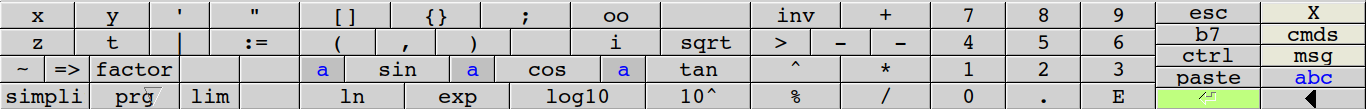
\includegraphics[width=\linewidth]{xcas-scientific-keyboard.png}
    \caption{\label{fig:xcas-scientific-keyboard}On-screen scientific keyboard in \xcas{}}
  \end{figure}
  Along the right hand side of the keyboard are some keys that can
  be used to change the keyboard.
  \begin{itemize}
  \item The \button{X} key hides the
    keyboard, just like pressing the \button{Kbd} button again.

  \item The \button{cmds} key toggles a menu bar at the bottom of the
    screen which can be used as an alternate menu or persistent
    submenu.  This bar will contain buttons \button{home},
    \button{<<}, some menu titles, \button{>>}, \button{var},
    \button{cust} and \button{X}.

    The \button{<<} and \button{>>} buttons scroll through menu
    items.  Clicking on one of the menu buttons will perform the
    appropriate action or replace the menu items by its submenu items.
    When submenu items appear, there will also be a \button{BACK}
    button to return to the previous menu.  Clicking on the
    \button{home} button returns the menu buttons to the main menu.

    After the menu buttons is a \button{var} button.  This replaces
    the menu buttons by buttons representing the variables that you
    have defined.  After that is a \button{cust} button, which
    displays commands that you store in a list variable \texttt{CST}
    (see section \ref{ssec:CST}).

    The last button, \button{X}, closes the menu bar.

  \item
    The \button{msg} key brings up a message window at the bottom
    of the window which will give you helpful messages; for example, if
    you save a graphic, it will tell you the name of the file it is
    saved in and how to include it in a \LaTeX{} file.

  \item The \button{abc} key toggles the keyboard between the
    scientific keyboard and an alphabetic keyboard.
  \end{itemize}

\item The button \button{X} closes the current session.
\end{itemize}

\section{Getting help}

\xcas{} is an extensive program, but using it is simplified with
several different ways of getting help.  The help menu (see section
\ref{ssec:helpmenu}) has several submenus for various forms of help,
some of which are mentioned below.

\subsection{Tooltips\label{ssec:ttips}}

If you hover the mouse cursor over certain parts of the \xcas{}
window, a temporary window will appear with information about the
part.  For example, if you move the mouse cursor over the status line,
you will get a message saying \textsf{Current CAS status. Click to
  modify}.

If you type a function name in the \xcas{} command line, a
similar temporary window will appear with information about the
function.

\subsection{\HTML{} help\label{sssec:htmlhelp}}

If you press the \textsf{F12} key, you will get a window which you can
use to search the html version of the manual.  You can also open this
window with the menu entry \textsf{Help\menusep{}Find word
  in HTML help}.

The \HTML{} help window has a search area; if you type a string in that
area you will be given a list of help topics that contain that string.
If you choose a topic and click \textsf{View}, your web browser will
show the appropriate page of the manual.


\subsection{Help index\label{sssec:helpind}}

If you click on the \button{?} button on the status line
you will get the help index.  You can also get the help index with the
menu item \textsf{Help\menusep{}Index}.

\begin{figure}\centering
  \includeimage[0.4142]{xcas-help-index-plotfunc.png}
  \caption{\label{fig:help-index}Help index in \xcas{}}
\end{figure}
The help index, shown in Figure~\ref{fig:help-index},
is a list of the \giac{} function and variable names.
You can scroll through the help index items and click on the word that
you want.  There is also a line in the help index window that you can
use to search the index; you can enter some text and be taken to the
part of the index with the words that begin with that text.
The \button{?} button next to this search line will open the \HTML{} help window.

If you select a function or variable name, a list of related words
(names of functions or variables) and a list of synonymous words will
appear in regions to the right.
Below the search line, there will be an area which will have a brief description
of the chosen term as well as how to call it.  If the term is a
command name, the calling sequence will be given as the command name
with the arguments within parentheses separated by commas.  Any
optional arguments will be shown within brackets.  In the window shown in
Figure~\ref{fig:help-index},
the first argument to \texttt{plotfunc} is an expression,
representing the function to be graphed.  There is an optional second
argument, which is either a variable name (which defaults to
\texttt{x}) or a vector of variable names for multivariable functions.
Finally, there is an optional third argument which can be used to
specify a color for the graph.

Below the brief description will be some entry fields that use
to enter the arguments.  If you fill them out and press the enter key,
the command with the arguments filled out will be put on the command
line.

Below the entry fields for the arguments will be a list of examples of
the command being used.  If you click on one of these examples, it
will be put on the command line.

A more thorough description of the function and its arguments is
available with the \button{Details}
button at the top of the help
index, which will open the relevant part of the manual in your
browser.  Alternatively, if you click on the \button{?}
button next to the search line, you will be taken to the \HTML{} help
window.

You can also open the help index in the following ways:
\begin{itemize}
\item
  You can press the tab key while typing in the \xcas{}
  command box.
  If you have entered part of a command name, you will be at the part
  of the index with words that begin with the text that you entered.

\item
  You can select a command from one of the menus.  If \texttt{Auto
    index help} is chosen (see \secref{sec:mconf}), then the help index
  will open with the command chosen.
\end{itemize}

\subsection{Getting help in a commandline}

You can get help from \xcas{} by using the
\texttt{findhelp}\index{findhelp@\texttt{findhelp}}
function.  If you enter \texttt{findhelp(}\textit{function}\texttt{)}
(or equivalently \texttt{?}~\textit{function}) at the command input,
where \textit{function} is the name of a \giac{} function, then
some notes on \textit{function} will appear in the answer portion and
the appropriate page of the manual will appear in your web browser.

\section{Menus}

The menus provide different ways to work with \xcas{} and its
sessions, as well as ways of inserting functions and constants into
the current session.  Selecting a menu item corresponding to a
function or constant brings up the help index (see section
\ref{sssec:helpind}) with the chosen function or constant selected.

\subsection{\textsf{File} menu}

The \textsf{File} menu contains commands that are used to save
sessions, save parts of sessions, and load previously saved sessions.
This menu contains the following entries:
\begin{description}
\item[New Session] ---
  This creates and opens a new session.
  The new session will be in a new tab, which will be labeled
  \textsf{Unnamed} until you save it (using the menu item
  \textsf{File\menusep{}Save} or the keystroke
  \textsf{Alt+S}).

\item[Open] ---
  This allows you to open a previously saved session.
  There will be a submenu with a list of saved session files in the
  primary directory (see \secref{ssec:wdir}) that you can open,
  as well as a \textsf{File} item which will open a directory browser
  use to find a session file.  This directory browser can also
  be opened with \textsf{Alt+O}.

\item[Import] ---
  This allows you to open a session that
  was created with the \Maple{} CAS, a \TI{}89 calculator or a \Voyage{}~200
  calculator.  You can execute this session with the
  \textsf{Edit\menusep{}Execute Session} menu entry, but it
  may be better to execute the commands one at a time to see if any
  modifications need to be done.

\item[Clone] ---
  This creates a copy of the current session in a Firefox
  interface; either using the server at
  \url{http://www-fourier.ujf-grenoble.fr/~parisse/xcasen.html}
  (\textsf{Online}) or a local copy (\textsf{Offline}).

\item[Insert] ---
  This allows you to insert a previously saved session, a link to a
  Firefox session, or a previously saved figure, spreadsheet or program.

\item[Save] (\textsf{Alt+S}) ---
  This saves the current session.

\item[Save as] ---
  This saves the current session under a name that you choose.

\item[Save all] ---
  This saves all currently opened sessions.

\item[Export as] ---
  This allows you to save the current session in different
  formats; either in \KhiCAS (which is \giac{} ported to run
  on various calculators) format, standard \xcas{} format, \xcas{}
  with \Python{} syntax format, \Maple{} format, \MuPAD{} format or \TI{}89 format.

\item[Kill] ---
  This kills the current session.

\item[Print] ---
  This allows you to create an image of the session in various ways.

  The \textsf{Preview} menu item saves an image of the current session in a file
  that you name.  The \texttt{To printer} item sends an image of the current
  session to the printer.  The \textsf{Preview selected levels} item
  saves the images of the commands and outputs of the selected levels,
  each in a separate file.

\item[LaTeX] ---
  This has submenu items that render the session in \LaTeX{} and give you the
  result in various ways.  The \texttt{LaTeX preview} menu item displays a
  compiled \LaTeX{} version of the current session.  The \textsf{LaTeX
    print} item saves a copy of the session in \LaTeX{} form, along with
  the compiled version in various formats.  The \texttt{LaTeX print
    selection} does the same as \textsf{LaTeX print}, but only for the
  selected levels.

\item[Screen capture] ---
  This creates a screenshot that can be saved in various formats.

\item[Quit and update Xcas] ---
  This quits \xcas{} after checking for a newer version.

\item[Quit] (\textsf{Ctrl+Q}) ---
  This quits \xcas{}.
\end{description}

\subsection{\textsf{Edit} menu}

The \textsf{Edit} menu contains commands that are used to execute and
undo parts of the current session.  This menu contains the following
entries:
\begin{description}
\item[Execute worksheet] (\textsf{Ctrl+F9}) ---
  This recalculates each level in the session.

\item[Execute worksheet with pauses] ---
  This recalculates each level in the session, pausing between
  calculations.

\item[Execute below] ---
  This recalculates the current level and each level below it.

\item[Remove answers below] ---
  This removes the answers to the current level and the levels
  below it.

\item[Undo] ---
  This undoes the latest edit done to the levels, including a
  deletion of a level.  It can be repeated to undo more than one edit.

\item[Redo] ---
  This redoes the undone editing.

\item[Paste] ---
  This pastes the contents of the system clipboard to the cursor
  position.

\item[Del selected levels] ---
  This deletes any entry levels that you have selected.

\item[selection$\,\to\,$LaTeX] (\textsf{Ctrl+T}) ---
  This puts a \LaTeX{} version of the
  selection (level, part of a level, or answer selected by clicking
  and dragging the mouse) on the system clipboard.

\item[New entry] (\textsf{Alt+N}) ---
  This inserts a new entry level above the current one.

\item[New parameter] (\textsf{Ctrl+P}) ---
  This brings up a window in which you can enter a name and
  conditions for a new parameter.

\item[Insert newline] ---
  This inserts a newline below the cursor.  Note that simply
  typing return will evaluate the current entry rather
  than inserting a newline.

\item[Merge selected levels] ---
  This merges the selected levels into a single level.
\end{description}

\subsection{\textsf{Cfg} menu}

The \textsf{Cfg} menu contains commands that are used to set the
behaviour of \xcas{}.  This menu contains the following entries:
\begin{description}
\item[CAS configuration] ---
  This opens a window that allows you to configure how
  \xcas{} performs calculations (see
  \secref{ssec:confcomp}).  This is the same window you
  get when you click on the status line.

\item[Graph configuration] ---
  This opens a window that allows you to configure the default
  settings for a graph (see \secref{ssec:confgraph}).
  This includes such things as the initial
  ranges of the variables.  Each graph also has a
  \button{cfg} button to configure the settings on a per graph basis.

\item[General configuration] ---
  This opens a window that allows you to configure various
  non-computational aspects of \xcas{}, such as the fonts, the
  default paper size, and the like (see \secref{sec:mconf}).

\item[Mode (syntax)] ---
  This changes the default syntax (see \secref{ssec:lang}).
  By default, \xcas{} uses its own syntax, but you can change it
  to \Python{} syntax, \Maple{} syntax, \MuPAD{} syntax or \TI{}89 syntax.

\item[Show] ---
  This displays parts of \xcas{}.
  \begin{description}
  \item[DispG] ---
    This shows the graphics display screen; which has
    all graphical commands from the session together on one screen.

  \item[keyboard] ---
    This shows the on-screen keyboard; the same as clicking on the
    \button{Kbd} button on the status line (see \secref{sec:swin},
    item \ref{enum:kbd}).

  \item[bandeau] ---
    This shows the menu buttons at the bottom of the window;
    the same as clicking on \button{cmds}
    on the on-screen keyboard
    (see \secref{sec:swin}, item \ref{enum:kbd}).

  \item[msg] ---
    This shows the messages window; the same as clicking on
    \textsf{msg} on the on-screen keyboard (see \secref{sec:swin},
    item \ref{enum:kbd}).
  \end{description}

\item[Hide] ---
  This hides the same items that you can show with \textsf{Show}.

\item[Index language] ---
  This allows you to choose a language in which to display the help index.

\item[Colors] ---
  This allows you to choose colors for various parts of the display.

\item[Session font] ---
  This allows you to choose a font for the sessions.

\item[All fonts] ---
  This allows you to choose fonts for the session, the main menu and
  the keyboard.

\item[browser] ---
  This allows you to choose a browser that \xcas{} will use when
  needed.  If this is blank, then \xcas{} will use its own
  internal browser.

\item[Save configuration] ---
  This saves the configurations that you chose with the
  \textsf{Cfg} menu or chose by clicking on the status line.
\end{description}

\subsection{\textsf{Help} menu\label{ssec:helpmenu}}

The \textsf{Help} menu contains commands that let you get information
about \xcas{} from various sources. This menu contains the
following entries:
\begin{description}
\item[Index] ---
  This brings up the help index (see \secref{sssec:helpind}).

\item[Find word in \HTML{} help] (\textsf{F12}) ---
  This brings up a page which helps you search for keywords in
  the html documentation that came with \xcas{} (see
  \secref{sssec:htmlhelp}).  The help will be displayed in your browser.

\item[Interface] ---
  This brings up a tutorial for the \xcas{} interface.  The
  tutorial will be displayed in your browser.

\item[Reference card, fiches] ---
  This brings up a pdf reference card for
  \xcas{}.  The card will be displayed in your browser.

\item[Manuals] ---
  This allows you to choose from a variety of manuals for \xcas{},
  which will appear in your browser.
  \begin{description}
  \item[CAS reference] ---
    This brings up the manual for \xcas{}.

  \item[Algorithmes (\HTML{})] ---
    This brings up a manual for the algorithms used by \xcas{}.

  \item[Algorithmes (PDF)] ---
    This brings up a pdf version of the manual for the algorithms
    used by \xcas{}.

  \item[Geometry] ---
    This brings up a manual for two-dimensional geometry in
    \xcas{}.

  \item[Programmation] ---
    This brings up a manual for programming in \xcas{}.

  \item[Simulation] ---
    This brings up a manual for statistics and using the
    \xcas{} spreadsheet.

  \item[Turtle] ---
    This brings up a manual for using the \textsf{Turtle} drawing
    screen in \xcas{}.

  \item[Exercices] ---
    This brings up a page of exercises that you can do with
    \xcas{}.

  \item[Amusement] ---
    This brings up a page of mathematical amusements that you can
    work through with \xcas{}.

  \item[PARI-GP] ---
    This brings up documentation for the GP/PARI functions.
  \end{description}

\item[Internet] ---
  The \texttt{Internet} menu contains menu items that take you to
  various web pages related to \xcas{}.  Among them are the
  following entries:
  \begin{description}
  \item[Forum] ---
    This takes you to the \xcas{} forum.

  \item[Update help] ---
    This installs updated help files (retrieved from the
    \xcas{} website).
  \end{description}
  There are also several menu items that take you to \xcas{} related pages written
  in French; namely:
  \begin{description}
  \item[Aide-memoire lycee] ---
    This takes you to a paper discussing \xcas{} and high
    school.

  \item[Documents pedagogiques lycee] ---
    This takes you to a page on the \xcas{} website with a
    list of useful links.

  \item[Documents algorithmique] ---
    This takes you to a page on the \xcas{} website with a
    list of links.

  \item[Site Lycee de G. Connan] ---
    This takes you to a page about a free book written by
    Guillaume Connan teaching algorithms to high school students.

  \item[Site Lycee de L. Briel] ---
    This takes you to a website about \xcas{} for high
    school students.

  \item[Calcul formel au lycee, par D. Chevallair] ---
    This takes you to a pdf file discussing the use of
    \xcas{} in high school.

  \item[Site de F. Han] ---
    This takes you to a website by Frederic Han about
    \xcas{} and a QT frontent for \giac{}.

  \item[Ressources Capes] ---
    This takes you to a website with various external sources.

  \item[Ressources Agregation externe] ---
    This takes you to a collection of external resources.

  \item[Ressources Agregation interne] ---
    This takes you to a page on the \xcas{} website.
  \end{description}

\item[Start with CAS] ---
  This menu has the following entries:
  \begin{description}
  \item[Tutorial] ---
    This opens up the tutorial.
  \item[Solutions] ---
    This opens up the solutions to the exercises in the tutorial.
  \end{description}

\item[Tutoriel algo] ---
  This opens up a tutorial on algorithms and programming with
  \xcas{}.

\item[Rebuild help cache] ---
  This rebuilds the help index.

\item[About] ---
  This displays a message window with information about \xcas{}.

\item[Examples] ---
  This allows you to choose from a variety of example worksheets,
  which will then be copied to your current directory and opened.
\end{description}

\subsection{\textsf{Toolbox} menu}

The \textsf{Toolbox} menu contains commands that are used to insert
operators into the session.  This menu includes the following entries:

\begin{description}
\item[New entry] (\textsf{Alt+N}) ---
  This inserts a new level.

\item[New comment] (\textsf{Alt+C}) ---
  This inserts a new comment level.
\end{description}
The other entries let you insert mathematical operations into
the current level. If \textsf{Auto index help} is chosen
(see \secref{sec:mconf}), then the help index will open
help index (see \secref{sssec:helpind})
with the chosen command selected.

\subsection{\textsf{Expression} menu}

The \textsf{Expression} menu contains commands that are used to
transform expressions.  The first entry is \textsf{Expression\menusep{}New expression}
(which is equivalent to \textsf{Alt+E}), which inserts a new level and
brings up the on-screen keyboard (see \secref{sec:swin}, item
\ref{enum:kbd}).  The rest of the entries can be used to insert
various transformations.

\subsection{\textsf{Cmds} menu}

The \textsf{Cmds} menu contains various \giac{} functions and
constants separated into categories.  If \textsf{Auto index help} is
chosen (see \secref{sec:mconf}), then when you select a function or
constant, the help index (see \secref{sssec:helpind}) opens with the
function or constant selected, which can be used to insert the entry
on the command line.  Otherwise, the constant or function will be
inserted on the command line.

\subsection{\textsf{Prg} menu}

The \textsf{Prg} menu contains commands that are used to write
\giac{} programs.  The first entry,
\textsf{Prg\menusep{}New program} (equivalent to
\textsf{Alt+P}), inserts a program level and brings up the program
editor (see \secref{ssec:proged}).The other entries are useful
commands for writing \giac{} programs.

\subsection{\textsf{Graphic} menu}

The \textsf{Graphic} menu contains commands that are used to create
graphs.  The first entry,
\textsf{Graphic\menusep{}Attributs} (equivalent to
\textsf{Alt+K}), brings up a window containing different attributes of
the graph (such as line width, color, etc.).  The other entries are
commands for creating and manipulating graphs.

\subsection{\textsf{Geo} menu}

The \textsf{Geo} menu contains commands that are used to work with
two- and three-dimensional geometric figures.  The first two entries,
\textsf{Geo\menusep{}New figure 2d} (equivalent to
\textsf{Alt+G}) and \textsf{Geo\menusep{}New figure 3d}
(equivalent to \textsf{Alt+H}) create levels for two- and
three-dimensional figures, respectively. (See
\secref{sec:graphscreen}.) The other menu items are for working with
the figures.

\subsection{\textsf{Spreadsheet} menu}

The \textsf{Spreadsheet} menu contains commands that are used to work
with spreadsheets.  (See See \secref{sec:spreadsheet}.) The first menu
item, \textsf{Spreadsheet\menusep{}New spreadsheet}
(equivalent to \textsf{Alt+T}), brings up a window where you can set
the size and other attributes of a spreadsheet, after which one will
be created.  The submenus contain commands for working with
spreadsheets.  Notice that the spreadsheet itself will have menus that
are the same as these submenus.

\subsection{\textsf{Phys} menu}

The \textsf{Phys} menu contains submenus with various categories of
constants, as well as functions for converting units.

\subsection{\textsf{Highschool} menu}

The \textsf{Highschool} menu contains computer algebra commands that
are useful at different levels of highschool.  There is also a
\textsf{Program} submenu with some program control functions.

\subsection{\textsf{Turtle} menu}

The \textsf{Turtle} menu contains the commands that are used to create
and control a Turtle screen.  The first menu item,
\textsf{Turtle\menusep{}New turtle}, creates a Turtle
drawing screen.  The other menu items contain commands for working
with the screen.

\section{Configuring \xcas{}\label{sec:config}}

\subsection{Number of significant digits
  \label{ssec:sigdig}}

By default, \xcas{} uses and displays 12 significant
digits, but you can set the number of digits to other positive
integers.  If you set the number of significant digits to a number
less than 14, then \xcas{} will use the computer's
floating point hardware, and so calculations will be done to more
significant digits than you asked for, but only the number of digits
that you asked for will be displayed.  If you set the number of
significant digits to 14 or higher, then both the
computations and the display will use that number of digits.

You can set the number of significant digits for \xcas{} by
using the CAS configuration screen (see \secref{ssec:confcomp}).  The
number of significant digits is stored in the variable
\texttt{DIGITS}\index{DIGITS@\texttt{DIGITS}}
or \texttt{Digits}\index{Digits@\texttt{Digits}},
so you can also set it by giving the variable
\texttt{DIGITS} a new value, as in \texttt{DIGITS:=20}.  The value
will be stored in the configuration file (see \secref{ssec:conffile}),
and so can also be set there.

\subsection{Language mode\label{ssec:lang}}

\xcas{} has its own language which it uses by default, but you
can also use either \Python{} (with the option having the \texttt{\^{}}
character represent either exponentiation or the \textsl{exclusive or}
operator) or the language used by \Maple{}, \MuPAD{}, or the
\TI{}89 calculator.

You can set which language \xcas{} uses in the CAS configuration
screen (see \secref{ssec:confcomp}). You can also set the language
with the \texttt{xcas\_mode}\index{xcas\_mode@\texttt{xcas\_mode}} command.
\begin{itemize}
\item The \texttt{xcas\_mode} command takes
  an integer: 0, 1, 2, 3, 256 or 512.
  \begin{itemize}
  \item \texttt{xcas\_mode(0)}
    to use the \xcas{} language.
  \item  \texttt{xcas\_mode(1)}
    to use the \Maple{} language.
  \item \texttt{xcas\_mode(2)}
    to use the \MuPAD{} language.
  \item \texttt{xcas\_mode(3)}
    to use the \TI{}89 language.
  \item \texttt{xcas\_mode(256)}
    to use the \Python{} language with \texttt{\^{}} representing exponentiation.
  \item \texttt{xcas\_mode(512)}
    to use the \Python{} language with \texttt{\^{}} representing
    \textsl{exclusive or}.
  \end{itemize}
\end{itemize}
The language you choose will be stored in the configuration file (see
\secref{ssec:conffile}), and so can also be set there.

\subsection{Units for angles\label{ssec:angles}}

By default, \xcas{} assumes that any angles you use (for
example, as the argument to a trigonometric function) are being
measured in radians.  If you want, you can have \xcas{} use
degrees.

You can set which angle measure \xcas{} uses in the CAS
configuration screen (see \secref{ssec:confcomp}). Your choice will be
stored in the variable \texttt{angle\_radian}\index{angle\_radian@\texttt{angle\_radian}};
this will be \texttt{1} if you measure your angles in radians and \texttt{0}
if you measure your angles in degrees.  You can also change which angle measure you
use by setting the variable \texttt{angle\_radian} to the appropriate
value.  The angle measure you want to use will be stored in the
configuration file (see \secref{ssec:conffile}), and so can also be
set there.

\subsection{Exact or approximate values\label{ssec:approx}}

Some numbers, such as $\pi$ and $\sqrt{2}$, cannot be written down
exactly as decimal numbers.  When computing with such numbers, by
default \xcas{} leaves them in exact, symbolic form.  If you
want, you can have \xcas{} automatically give you decimal
approximations for these numbers.

You can set whether or not \xcas{} gives you exact or
approximate values by using the CAS configuration screen (see
\secref{ssec:confcomp}).  Your choice will be stored in the variable
\texttt{approx\_mode}\index{approx\_mode@\texttt{approx\_mode}},
where a value of 0 means that \xcas{}
will give you exact answers when possible and a value of 1 means that
\xcas{} will give you decimal approximations.  Your choice will
be stored in the configuration file (see section \ref{ssec:conffile}),
and so can also be set there.

\subsection{Complex numbers\label{ssec:complex}}

When factoring polynomials (see \secref{ssec:factore}), by default
\xcas{} won't introduce complex numbers if they aren't already
being used.  For example,
\begin{xcasinput}
factor(x^2+2)
\end{xcasinput}
simply returns
\begin{xcasoutput}
  x^{2}+2
\end{xcasoutput}
but if an expression already involves complex numbers then
\xcas{} uses them:
\begin{xcasinput}
factor(i*x^2+2*i)
\end{xcasinput}
\begin{xcasoutput}
  \left(x-\mathrm{i} \sqrt{2}\right) \left(\mathrm{i} x-\sqrt{2}\right)
\end{xcasoutput}

\xcas{} can also find complex roots when complex
numbers are not present; for example, the command
\texttt{cfactor}\index{cfactor@\texttt{cfactor}}
(see \secref{ssec:factore}) or \texttt{cFactor}\index{cFactor@\texttt{cFactor}}
command factors over the complex numbers. For example:
\begin{xcasinput}
cfactor(x^2+2)
\end{xcasinput}
\begin{xcasoutput}
  \left(x+\mathrm{i} \sqrt{2}\right) \left(x-\mathrm{i} \sqrt{2}\right)
\end{xcasoutput}

If you want \xcas{} to use complex numbers by default, you can
turn on complex mode.  In complex mode, the command line
\begin{xcasinput}
factor(x^2+2)
\end{xcasinput}
returns
\begin{xcasoutput}
  \left(x+\mathrm{i} \sqrt{2}\right) \left(x-\mathrm{i} \sqrt{2}\right)
\end{xcasoutput}

You can turn on complex mode from the CAS configuration screen (see
\secref{ssec:confcomp}).  This mode is determined by the value of the
variable \texttt{complex\_mode}\index{complex\_mode@\texttt{complex\_mode}};
if this is \texttt{1} then complex
mode is on, if this is \texttt{0} then complex mode is off. This
option will be stored in the configuration file (see
\secref{ssec:conffile}), and so can also be set there.

\subsection{Complex variables\label{ssec:cvars}}

By default, new variables are assumed to be real; functions which work
with the real and imaginary parts of variables will assume that a
variable is real.  For example, \texttt{re} returns the real part of
its argument and \texttt{im} returns the imaginary part (see
\secref{ssec:reim}), and so
\begin{xcasinput}
re(z)
\end{xcasinput}
returns $z$ and
\begin{xcasinput}
im(z)
\end{xcasinput}
returns $0$.

If you want variables to be complex by default, you can have
\xcas{} use complex variable mode.  You can set this from the
CAS configuration screen (see \secref{ssec:confcomp}).  Your choice
will be stored in the variable
\texttt{complex\_variables}\index{complex\_variables@\texttt{complex\_variables}},
where a value of 0 means that \xcas{} will assume that variables are
real and and a value of 1 means that \xcas{} will assume that
variables are complex.  Your choice will be stored in the
configuration file (see \secref{ssec:conffile}), and so can also be
set there.

\subsection{Configuring the computations\label{ssec:confcomp}}

You can configure how \xcas{} computes by using the menu item
\textsf{Cfg\menusep{}CAS configuration} or by clicking on
the status line.  This will open a window with the following options:
\begin{description}
\item[Prog style] (default: \xcas{}) ---
  This has a menu from which you can choose a different language
  to program in; you can choose from \xcas{}, \texttt{Python
    \^{}==**} (\Python{} syntax, except that \texttt{\^{}} will be the
  exponentiation operator as in \xcas{} rather than the
  \textsl{exclusive or} operator as in \Python{}), \texttt{Python \^{}==xor}
  (\Python{} syntax, where \texttt{\^{}} is the \textsl{exclusive or} operator),
  \Maple{}, \MuPAD{} and \TI{}89/92.

\item[eval] (default: 25) ---
  Here you can input a positive integer specifying the maximum number
  of recursions allowed when evaluating expressions.

\item[prog] (default: 1) ---
  Here you can input a positive integer
  specifying the maximum number of recursions allowed when executing
  programs.

\item[recurs] (default: 100) ---
  Here you can input a positive integer
  specifying the maximum number of recursive calls.

\item[debug] (default: 0) ---
  Here you can input a 0 or 1.  If this is 1, then
  \xcas{} will display intermediate information on the
  algorithms used by \xcas{}.  If this is 0, then no such
  information is displayed.

\item[maxiter]\label{enum:maxiter}  (default: 20) ---
  Here you can input an integer specifying
  the maximum number of iterations to be used in Newton's method.

\item[Float format]\label{enum:float}  (default: \texttt{standard}) ---
  This has a menu from which you can choose how to display
  decimal numbers.  Your choices will be:
  \begin{description}
  \item[standard]  In standard notation, a number will be
    written out completely without using exponentials; for example,
    \texttt{15000.12} will be displayed as \texttt{15000.12}.
  \item[scientific]  In scientific notation, a number will be
    written as a number between 1 and 10 times a power of ten; for example,
    \texttt{15000.12} will be displayed as \texttt{1.500012000000e+04}
    (where the number after \texttt{e} indicates the power of 10).
  \item[engineer]  In engineering notation, a number will be
    written as a number between 1 and 1000 times a power of ten, where
    the power of 10 is a multiple of three.  For example,
    \texttt{15000.12} will be displayed as \texttt{15.00012e3}.
  \end{description}

\item[Digits]\label{enum:digs}  (default: 12) ---
  Here you can input a positive integer which will
  indicate the number of significant digits that \xcas{} will use.

\item[epsilon]\label{enum:eps}  (default: $10^{-12}$) ---
  Here you can input a floating point number
  which will be the value of epsilon used by \texttt{epsilon2zero},
  which is a function that replaces numbers with absolute value less
  than epsilon by 0 (see \secref{ssec:epsilon2zero}).

\item[proba]  (default: $10^{-15}$) ---
  Here you can input a floating point number.
  If this number is greater than zero, then in some cases
  \xcas{} can use probabilistic algorithms and give a result
  with probability of being false less than this value.  (One such
  example of a probabilistic algorithm that \xcas{} can use is
  the algorithm to compute the determinant of a large matrix with
  integer coefficients.)

\item[approx]  (default: unchecked) ---
  If checked, then exact
  numbers such as $\sqrt{2}$ will be given a floating point approximation,
  otherwise exact values will be used when possible.
  (See \secref{ssec:approx}.)

\item[autosimplify]  (default: 1) ---
  Here you can input 0, 1 or 2.  A value of 0
  means no automatic simplification will be done, a value of 1 means
  grouped simplification will be automatic.  A value of 2 means that
  all simplification will be automatic.

\item[threads]  (default: 1) ---
  Here you can enter a positive integer to
  indicate the number of threads (for a possible future threaded
  version).

\item[Integer basis]\label{enum:base}  (default: 10) ---
  This has a menu from which you can choose an integer base
  to work in; your choices will be 8, 10 and 16.

\item[radian] (default: checked) ---
  If checked, then angles will be measured in radians, otherwise they
  will be measured in degrees.

\item[Complex]  (default: unchecked) ---
  If checked, then \xcas{} will work in complex mode, meaning, for example, that
  polynomials will be factored with complex numbers if necessary.

\item[Cmplx\_var]  (default: unchecked) ---
  If checked, then variables will by default be assumed to be complex.
  For example, the expression \texttt{re(z)} won't be simplified, it will return
  \texttt{re(z)}.  If unchecked, then variables by default
  will be assumed to be real, and so \texttt{re(z)} will be
  simplified to \texttt{z}.

\item[increasing power]  (default: unchecked) ---
  If checked, then polynomials will be written out in increasing powers of the
  variable, otherwise they will be written in decreasing powers.

\item[All\_trig\_sol]\label{enum:trig}  (default: unchecked) ---
  If checked, then \xcas{} will give the complete solutions of
  trigonometric equations.  For example, the solution of $\cos x=0$
  will be given as $[(2n\_{0}\pi+\pi)/2]$, where $n_{0}$ can be any
  integer.  If unchecked, then only the primary solutions
  of trigonometric equations will be given.  For example, the
  solutions of $\cos(x)=0$ will be the pair $[-\pi/2,\pi/2]$.

\item[Sqrt]  (default: checked) ---
  If checked, then the \texttt{factor} command will factor second
  degree polynomials, even when the roots are not in the field determined by
  the coefficients. For example:
\begin{xcasinput}
factor(x^2-3)
\end{xcasinput}
  \begin{xcasoutput}
    \left(x-\sqrt{3}\right) \left(x+\sqrt{3}\right)
  \end{xcasoutput}
  If unchecked, then the same command line returns $x^{2}-3$.
\end{description}
This page also has buttons for applying the settings, saving the
settings for future sessions, canceling any new settings, and restoring
the default settings.

\subsection{Configuring the graphics\label{ssec:confgraph}}

You can configure each graphics screen by clicking on the \texttt{cfg}
button on the graphics screen's control panel to the right of the
graph.  You can also change the default graphical configuration using
the the menu item \textsf{Cfg\menusep{}Graph
  configuration}. You will then be given a window in which you can
change the following options:
\begin{itemize}
\item \texttt{X-} and \texttt{X+}:
  these determine the $x$ values for which calculations will be done.

\item \texttt{Y-} and \texttt{Y+}:
  these determine the $y$ values for which calculations will be done.

\item \texttt{Z-} and \texttt{Z+}:
  these determine the $z$ values for which calculations will be done.

\item \texttt{t-} and \texttt{t+}:
  these determine the $t$ values for which calculations will be
  done (when plotting parametric curves, for example).

\item \texttt{WX-} and \texttt{WX+}:
  these determine the range of $x$ values for the viewing window.

\item \texttt{WY-} and \texttt{WY+}:
  these determine the range of $y$ values for the viewing window.

\item \texttt{TX} and \texttt{TY}:
  these determine the tick ranges on the $x$- and $y$-axes.

\item \texttt{class\_min}:
  this determines the minimum size of a statistics class.

\item \texttt{class\_size}:
  this determines the default size of a statistics class.

\item \texttt{autoscale}:
  when checked, the graphic will be autoscaled.

\item \texttt{ortho}:
  when checked, all axes of the graphic will be scaled equally.

\item \texttt{>W} and \texttt{W>}:
  these are convenient shortcuts to copy the \texttt{X-}, \texttt{X+},
  \texttt{Y-} and \texttt{Y+} values to  \texttt{WX-}, \texttt{WX+},
  \texttt{WY-} and \texttt{WY+}, or the other way around.
\end{itemize}
Note that the viewing window is not the same as the calculation
window; if the calculation window is larger than the visible window,
then you can scroll to bring other parts of the calculation into view.

This page also has buttons for applying the settings, saving the
settings for future sessions, or canceling any new settings.

\subsection{More configuration\label{sec:mconf}}

You can configure other aspects of \xcas{} (besides the
computational aspects and graphics) using the the menu item
\textsf{Cfg\menusep{}General configuration}. You will then
be given a window in which you can change the following options:
\begin{description}
\item[Font] ---
  This lets you choose a session font, the same as choosing the menu
  item \textsf{Cfg\menusep{}Session font}.

\item[Level] ---
  This determines what type of level should be open when you start
  a new session.

\item[browser] ---
  This determines what browser \xcas{} will use when it
  requires one, for example when displaying help.  If this is empty,
  \xcas{} will use its built-in browser.

\item[Auto \HTML{} help] ---
  If checked, then whenever you choose a function from a menu,
  a help page for that function will appear in your browser.
  Regardless of whether this box is checked or not, the help page will
  also appear in your browser if you enter \texttt{?} \textit{function}
  from a command box.

\item[Auto index help] ---
  If checked, then whenever you choose a command from a
  menu, the help index page for that function will appear.  This is
  the same page you get when you choose the command from the help
  index.  (See \secref{sssec:helpind}.)

\item[Print format] ---
  This determines the paper size for printing and saving files.
  There is also a button use to have the printing done in
  landscape mode; if this button is not checked, the printing will be
  done in portrait.

\item[Disable Tool tips] ---
  If checked, \xcas{} will stop displaying tool tips
  (see \secref{ssec:ttips}).

\item[rows, columns] ---
  These determine the default number of rows and columns for the
  matrix editor and spreadsheet (see \secref{sec:spreadsheet}).

\item[PS view] ---
  This determines what program is used to preview Postscript files.

\item[Step by step] ---
  If checked, then \xcas{} will not save context information.

\item[Proxy] ---
  This sets a proxy server for updates.
\end{description}

\subsection{Configuration file\label{ssec:conffile}}

When you save changes to your configuration, they are stored in a
configuration file, which will be \texttt{.xcasrc}\index{.xcasrc@\texttt{.xcasrc}} in
your home directory in Unix and \texttt{xcas.rc}\index{xcas.rc@\texttt{xcas.rc}} in
Windows.  This file will have four functions --
\texttt{widget\_size}\index{widget\_size@\texttt{widget\_size}},
\texttt{cas\_setup}\index{cas\_setup@\texttt{cas\_setup}},
\texttt{xcas\_mode}\index{xcas\_mode@\texttt{xcas\_mode}} and
\texttt{xyztrange}\index{xyztrange@\texttt{xyztrange}} --
which determine the configuration and which are evaluated when
\xcas{} starts.

The \texttt{widget\_size} command sets properties of the opening
\xcas{} window.
\begin{itemize}
\item
  \texttt{widget\_size} takes between 1 and 12 arguments. The arguments
  (in order) are:
  \begin{description}
  \item[Font size.]  The first argument is a positive integer
    specifying the font size.  Optionally, this can be a bracketed list
    whose first number indicates the font and the second the font size.
  \item[Horizontal and vertical offset.]  The second and third
    arguments are horizontal and vertical distances in pixels from the
    upper left hand corner of the screen.   They specify where the upper
    left corner of the \xcas{} window is when it opens.
  \item[Window size.]  The fourth and fifth arguments specify the width and height in
    pixels of the \xcas{} window when it opens.
  \item[Keyboard] (see \secref{sec:swin}, item
    \ref{enum:kbd}).  The sixth argument is either 0 or 1; a 1 indicates
    that the on-screen keyboard will be open when \xcas{} starts,
    a 0 indicates that the keyboard will be hidden.
  \item[Open browser.] The seventh argument is either 0 or 1;
    a 1 indicates that the browser will be automatically opened to
    display help for the selected command in the menu or index, a 0
    indicates that the browser will not be automatically opened.
  \item[Message window] (see \secref{sec:swin}, item \ref{enum:kbd}).
    The eighth argument is either 0 or 1;
    a 1 indicates that \xcas{} will open with the message window,
    a 0 indicates that \xcas{} will open without the message
    window.
  \item[<empty>.] The ninth argument is currently not used.
  \item[Browser name.] The tenth argument is a string with the
    name of the browser to use to read the help pages.  A value of
    \texttt{"builtin"} means that \xcas{} will use a small browser
    built into \xcas{}.
  \item[Starting level] (see \secref{sec:levels}).  The eleventh
    argument indicates what level \xcas{} will start at; a 0
    means command line, a 1 means program editor, a
    2 means spreadsheet, and a 3 means a 2D geometry screen.
  \item[Postscript previewer.] The twelfth argument is a
    string with the name of a program for postscript previews; for
    example, \texttt{"gv"}.
  \end{description}
\end{itemize}

The \texttt{cas\_setup} command determines how computations will be
performed.
\begin{itemize}
\item
  \texttt{cas\_setup} takes nine arguments. The arguments (in
  order) are:
  \begin{description}
  \item[Approximate mode] (see \secref{ssec:approx}).  A 1
    means \xcas{} works in approximate mode, a 0 means exact mode.
  \item[Complex variables] (see \secref{ssec:complex}).  A 1
    means \xcas{} works with complex variables, a 0 means real
    variables.
  \item[Complex mode] (see \secref{ssec:complex}).
    A 1 means \xcas{} works with in complex mode, a 0 means real
    mode.
  \item[Radian] (see \secref{ssec:angles}).  A 1 means work in
    radians, a 0 means work in degrees.
  \item[Display format] (see \secref{ssec:confcomp}, item
    \ref{enum:float}).  A 0 means use the standard format to display
    numbers, a 1 means use scientific format, a 2 means use engineering
    format, and a 3 means use floating hexadecimal format (which is
    standardized with a non-zero first digit).
  \item[Epsilon] (see \secref{ssec:confcomp}, item
    \ref{enum:eps}).  This is the value of \texttt{epsilon} used
    by \xcas{}.
  \item[Digits.]  This is the number of digits to use to
    display a float.
  \item[Tasks.]  This will be used in the future for
    parallelism.
  \item[Increasing power.]  This is 0 to display polynomials
    in increasing power, and 1 to display polynomials in decreasing powers.
  \end{description}
\end{itemize}

The \texttt{xcas\_mode} command sets the computer language used by
  \xcas{} (see \secref{ssec:lang}).

The \texttt{xyztrange} command sets or returns the values of the
  graphics configuration.
\begin{itemize}
\item
  To set the values, \texttt{xyztrange} takes 15 arguments:
  \begin{itemize}
  \item \textit{x--} and \textit{x+}, the beginning and the end of the
    $x$ interval for which calculations will be done.
  \item \textit{y--} and \textit{y+}, the beginning and the end of the
    $y$ interval for which calculations will be done.
  \item \textit{z--} and \textit{z+}, the beginning and the end of the
    $z$ interval for which calculations will be done.
  \item \textit{t--} and \textit{t+}, the beginning and the end of the
    $t$ interval for which calculations will be done, when plotting
    parametric curves, for example.
  \item \textit{wx--} and \textit{wx+}, the beginning and the end of
    the $x$ values for the viewing window.
  \item \textit{wy--} and \textit{wy+}, the beginning and the end of
    the $y$ values for the viewing window.
  \item \textit{show\_axes}, to determine whether axes are shown or
    hidden (\texttt{1} to show, \texttt{0} to hide).
  \item \textit{class\_min}, the minimum size of a statistics class.
  \item \textit{class\_size}, the default size of a statistics class.
  \end{itemize}
\item
  \texttt{xyztrange(}$\textit{x--},\textit{x+},\textit{y--},\textit{y+},\textit{z--},\textit{z+},
  \textit{t--},\textit{t+},\textit{wx--},\textit{wx+},\textit{wy--},\textit{wy+},\textit{show\_axes},
  \textit{class\_min},\textit{class\_size}$\texttt{)}
  sets the parameters to the given values.
  
  Note that the viewing window is not the same as the calculation
  window; if the calculation window is larger than the visible window,
  then you can scroll to bring other parts of the calculation window
  into view.
\item To return the values, \texttt{xyztrange} takes no arguments.
\item \texttt{xyztrange()} returns a matrix where each row consists
  of a short description of the first twelve arguments along with
  their values.
\end{itemize}

\section{Printing and saving}

\subsection{Saving a session\label{ssec:sesssave}}

Each tab above the status line represents a session, the tab for the
active session will be yellow.  The label of each tab will be the name
of the file that the session is saved in; if the session hasn't been
saved the tab will read \textsf{Unnamed}.

You can save your current session by clicking on the \button{Save}
button on the status line.  If the session contains unsaved changes
the \button{Save} button will be red; the button will be green when
nothing needs to be saved.  The first time that you save a session you
will be prompted for a file name; you should choose a name that ends
in \texttt{.xws}.  Subsequent times that you save a session it will be
saved in the same file; to save a session in a different file you can
use the menu item \textsf{File\menusep{}Save as}.

If you have a session saved in a file and you want to load it in a
tab, use the menu item \textsf{File\menusep{}Open}.
From there you can choose a specific file from a list or open a
directory browser that use to choose a file.  The directory
browser can also be opened with \textsf{Alt+O}.

\subsection{Saving a spreadsheet\label{ssec:spreadsave}}

If you have a spreadsheet in one of the levels, you can save it
separately from the rest of the session.

When a spreadsheet is inserted it will have menus next to the level
number.  The \textsf{Table} menu has items that let you save the
spreadsheet in different formats, as well as insert previously saved
spreadsheets.

You can save a spreadsheet with the
\textsf{Table\menusep{}Save sheet as text} menu item.  If
you select that, you will be prompted for a file name; you should
choose a file name that ends in \texttt{.tab}.  Once you save a
spreadsheet, there will be a button to the right of the menus which
use to save any changes you make.  If you want to save the
spreadsheet under a different name, use the
\textsf{Table\menusep{}Save as alternate filename} menu
entry.

You can save a spreadsheet in other formats.  The
\textsf{Table\menusep{}Save as CSV} menu item will save a
spreadsheet in a comma-separated values file, and the
\textsf{Table\menusep{}Save as mathml} menu item will save
the spreadsheet in as a \MathML{} file.

use the \textsf{Table} menu to insert previously saved
spreadsheets; the menu item \textsf{Table\menusep{}Insert}
will bring up a directory browser that use to select a file to
enter.

\subsection{Saving a program\label{ssec:progsave}}

You can open up a program editor (see \secref{ssec:proged}) with the
menu item \textsf{Prg\menusep{}New program} or with
\textsf{Alt+P}.  If you select this item, you will be prompted for
information to fill out a template for a program and then be left in
the program editor.

At the top of the program editor are menus and buttons, at the far
right will be a \button{Save} button that you can press to save the
program.  The first time you save a program, you will be prompted for
a file name; you should choose a name ending in \texttt{.cxx}.  Once a
program is saved, the file name will appear to the right of the
\button{Save} button.  If you want to save the program under a
different name, use the \textsf{Prog\menusep{}Save
  as} item from the program editor menu.

To insert a previously saved program, use the
\textsf{Prog\menusep{}Load} item from the program editor
menu.

\subsection{Printing a session\label{ssec:printing}}

You can print a session with the
\textsf{File\menusep{}Print\menusep{}To printer}
menu item.

If you prefer to save the printed form as a file, use the
\textsf{File\menusep{}Print\menusep{}Preview}
menu item.  You will prompted for a file name to save the printed form
in; the file will be a PostScript file, so the name should end in
\texttt{.ps}. If you only want to save certain levels in printable
form, use the
\textsf{File\menusep{}Print\menusep{}Preview
  selected levels} menu item; this file will be encapsulated PostScript,
so the name should end in \texttt{.eps}.

\section{Translating to other computer languages}

\xcas{} can export a session, or parts of a session, to typesetting
languages such as \LaTeX{} and \MathML{}.

\subsection{Translating an expression to \LaTeX{}}

The \texttt{latex}\index{latex@\texttt{latex}} command
translates expressions to \LaTeX{}\index{LaTeX}.
\begin{itemize}
\item \texttt{latex} takes
  \textit{expr}, an expression.
\item \texttt{latex(}\textit{expr}\texttt{)} returns the result of
  evaluating \textit{expr} written in the \LaTeX{} typesetting language.
  Note that the returned value is a string which typesets properly when
  inserted in a (displayed) math environment.
  \item When copying the \texttt{latex} command output manually from
  a \giac{} interface to a \LaTeX{} document, be sure to remove the double quotes.
\end{itemize}

\subsubsection*{Example}
\begin{xcasinput}
latex(1+1/2)
\end{xcasinput}
\begin{xcasoutput}
  \text{$\backslash$frac\{3\}\{2\}}
\end{xcasoutput}

\subsection{Translating the entire session to \LaTeX{}}

To export entire session to a \LaTeX{}\index{LaTeX} file, use
the menu item \textsf{File\menusep{}LaTeX\menusep{}LaTeX~preview}.

\subsection{Translating graphical output to \LaTeX{}\label{ssec:graph2tex}}

You can see all of your graphic output at once on the
\texttt{DispG}\index{DispG@\texttt{DispG}} screen, which you can bring up with the
command \texttt{DispG()}.  (This screen can be cleared with the
command line command \texttt{erase()}.) On the \texttt{DispG} screen
there will be a \textsf{Print} menu; the
\textsf{Print\menusep{}LaTeX print} will give you several
files \texttt{DispG.tex}, \texttt{DispG.dvi}, \texttt{DispG.ps} and
\texttt{DispG.png} with the graphics in different formats. To save it
without using the \texttt{DispG()} command use the
\texttt{graph2tex}\index{graph2tex@\texttt{graph2tex}} command.

The \texttt{graph2tex} command saves all current graphic output to a
\LaTeX{}\index{LateX} file.
\begin{itemize}
\item \texttt{graph2tex} takes
  \textit{filename}\texttt{.tex}, the name of a file.
\item
  \texttt{graph2tex("}\textit{filename}\texttt{.tex")}
  saves all graphic output in \LaTeX{} form to the file
  \textit{filename}\texttt{.tex}.
\end{itemize}

\subsubsection*{Example}
The command line
\begin{xcasinput}
graph2tex("myfile.tex")
\end{xcasinput}
creates a \LaTeX{} file \texttt{myfile.tex} with the graphs.
To save a 3D graph, use the command
\texttt{graph3d2tex}\index{graph3d2tex@\texttt{graph3d2tex}}.


To save a single graph as a \LaTeX{} file, use the \textsf{M}
menu to the right of the graph.  Selecting
\textsf{M\menusep{}Export Print\menusep{}Print
  (with LaTeX)} will save the current graph.  You can also save a single
graph by selecting that level, then use the menu item
\textsf{File\menusep{}LaTeX\menusep{}LaTeX print
  selection}.  This method will save the graph in several formats;
\textit{sessionname}\texttt{.tex}, \textit{sessionname}\texttt{.dvi},
\textit{sessionname}\texttt{.ps} and
\textit{sessionname}\texttt{.png}.  If the session has not been saved
and named, the files will begin with \texttt{session}\textit{n} for
some integer \textit{n}.

\subsection{Translating an expression to \MathML{}}

The \texttt{mathml}\index{mathml@\texttt{mathml}}
command translates expressions to \MathML{}\index{MathML}.
\begin{itemize}
\item \texttt{mathml} takes
  \textit{expr}, an expression.
\item \texttt{mathml(}\textit{expr}\texttt{)} returns the result of
  evaluating \textit{expr} written in \MathML{}.
\end{itemize}

\subsubsection*{Example}
\begin{xcasinput}
mathml(1/4+1/4)
\end{xcasinput}
\begin{lstlisting}[language=XML]
<?xml version="1.0" encoding="iso-8859-1"?>
<!DOCTYPE html PUBLIC "-//W3C//DTD XHTML 1.1 plus MathML 2.0//EN"
"http://www.w3.org/TR/MathML2/dtd/xhtml-math11-f.dtd" [
<!ENTITY mathml "http://www.w3.org/1998/Math/MathML">
]>
<html xmlns="http://www.w3.org/1999/xhtml">
<body>

<math mode="display" xmlns="http://www.w3.org/1998/Math/MathML">

<mfrac><mrow><mn>1</mn></mrow><mrow><mn>2</mn></mrow></mfrac>

</math><br/>

</body> </html>
\end{lstlisting}
This is the number $1/2$ in \MathML{} form, along with enough
information to make it a complete \HTML{} document.

\subsection{Translating a spreadsheet to \MathML{}\label{ssec:spread2mathml}}

You can translate an entire spreadsheet to \MathML{}\index{MathML} with the spreadsheet
menu command \textsf{Table\menusep{}Save as MathML}.

\subsection{Indent an \XML{} string\label{ssec:xmlpr}}

The \texttt{xml\_print}\index{xml\_print@\texttt{xml\_print}}
command formats an \XML{} string.
\begin{itemize}
\item \texttt{xml\_print} takes
  \textit{str}, a string, assumed to contain \XML{}.
\item \texttt{xml\_print(}\textit{str}\texttt{)} returns a string with the \XML{} code
  indented for better readability. The default indentation is two spaces.
\end{itemize}

\subsubsection*{Example}
\begin{xcasinput}
xml_print("<?xml version='1.0'?><r><c1>bla</c1><c2></c2><c3/></r>")
\end{xcasinput}
\begin{lstlisting}[language=XML]
<?xml version='1.0'?>
<r>
  <c1>bla</c1>
  <c2></c2>
  <c3/>
</r>
\end{lstlisting}

\subsection{Export to presentation or content \MathML{}
  \label{ssec:exportMathML}}

You can translate the result of an expression into various
types of \MathML{}\index{MathML} with the
\texttt{export\_mathml}\index{export\_mathml@\texttt{export\_mathml}} command.
\begin{itemize}
\item \texttt{export\_mathml} takes one mandatory argument and one optional
  argument:
  \begin{itemize}
  \item \textit{expr}, an expression.
  \item Optionally, \textit{format}, which can be \texttt{content} or
    \texttt{display}, specifying the output format.
  \end{itemize}
\item
  \texttt{export\_mathml(}$\textit{expr}\,\langle,\textit{format}\,\rangle$\texttt{)}
  returns the result of evaluating \textit{expr} written in \MathML{}, with a single
  \texttt{math} block which will be a \texttt{semantics} block.
  Choices for the second argument are:
  \begin{itemize}
  \item None: the \texttt{semantics} block will
    contain both presentation and content \MathML{}.
  \item \texttt{content}: the
    \texttt{semantics} block will contain only the content \MathML{}.
  \item \texttt{display}: the
    \texttt{semantics} block will contain only the presentation \MathML{}.
  \end{itemize}
\end{itemize}

\subsubsection*{Examples}
\begin{xcasinput}
xml_print(export_mathml(a+2*b))
\end{xcasinput}
\begin{lstlisting}[language=XML]
<math mode='display' xmlns='http://www.w3.org/1998/Math/MathML'>
  <semantics>
    <mrow xref='id5'>
      <mi xref='id1'>a</mi>
      <mo>+</mo>
      <mrow xref='id4'>
        <mn xref='id2'>2</mn>
        <mo>&it;</mo>
        <mi xref='id3'>b</mi>
      </mrow>
    </mrow>
    <annotation-xml encoding='MathML-Content'>
      <apply id='id5'>
        <plus/>
        <ci id='id1'>a</ci>
        <apply id='id4'>
          <times/>
          <cn id='id2' type='integer'>2</cn>
          <ci id='id3'>b</ci>
        </apply>
      </apply>
    </annotation-xml>
    <annotation encoding='giac'>a+2*b</annotation>
  </semantics>
</math>
\end{lstlisting}
\begin{xcasinput}
xml_print(export_mathml(a+2*b,content))
\end{xcasinput}
\begin{lstlisting}[language=XML]
<math mode='display' xmlns='http://www.w3.org/1998/Math/MathML'>
  <apply id='id5'>
    <plus/>
    <ci id='id1'>a</ci>
    <apply id='id4'>
      <times/>
      <cn id='id2' type='integer'>2</cn>
      <ci id='id3'>b</ci>
    </apply>
  </apply>
</math>
\end{lstlisting}
\begin{xcasinput}
xml_print(export_mathml(a+2*b,display))
\end{xcasinput}
\begin{lstlisting}[language=XML]
<math mode='display' xmlns='http://www.w3.org/1998/Math/MathML'>
  <mrow>
    <mi>a</mi>
    <mo>+</mo>
    <mrow>
      <mn>2</mn>
      <mo>&it;</mo>
      <mi>b</mi>
    </mrow>
  </mrow>
</math>
\end{lstlisting}
\begin{xcasinput}
s:=export_mathml(1/(x^2+1),display):;
xml_print(s)
\end{xcasinput}
\begin{lstlisting}[language=XML]
<math mode='display' xmlns='http://www.w3.org/1998/Math/MathML'>
  <mfrac>
    <mn>1</mn>
    <mrow>
      <msup>
        <mi>x</mi>
        <mn>2</mn>
      </msup>
      <mo>+</mo>
      <mn>1</mn>
    </mrow>
  </mfrac>
</math>
\end{lstlisting}

\subsection{Configuring markup export}

Export to \LaTeX{}, \MathML{} and \TeXmacs{} Scheme has
some configuration options that can be set by using the \texttt{markup\_cfg}
command. This applies to \texttt{latex} and \texttt{export\_mathml} commands
as well as to \TeXmacs{} sessions (note that \texttt{mathml} command does
not support this configuration).
\begin{itemize}
  \item \texttt{markup\_cfg} takes a sequence of one or more arguments,
  each of which being one of:
  \begin{itemize}
    \item \texttt{simplify=[}\textit{simp}\texttt{]}, where \textit{simp} is
    a sequence containing one or more of the following: \texttt{product},
    \texttt{apply}, or \texttt{pow}. If \textit{simp} has only one element,
    square brackets may be omitted.
    \item \texttt{mathml=[}\textit{comp}\texttt{]}, where \texttt{comp} is
    a sequence of one or more of the following: \texttt{display} or
    \texttt{content}. If \textit{comp} has only one element,
    square brackets may be omitted.
  \end{itemize}
  \item \texttt{markup\_cfg} returns 1 if the configuration is successful,
  else it returns 0.
  \item The \texttt{simplify} argument refers to enabling/disabling automatic
  simplification of mathematical notation. Precisely:
  \begin{itemize}
    \item Multiplication is made implicit where possible,
    hence the export commands favor e.g.~$2x$ instead of $2\cdot x$.
    If \textit{simp} contains \texttt{product}, then
    implicit multiplication is allowed, else it is not allowed (in that case
    the $\cdot$ symbol is always inserted).
    \item Parentheses are omitted from function application when possible,
    i.e.~when the argument is sufficiently simple. Therefore the
    export commands favor e.g.~$\sin x$ instead of $\sin(x)$.
    If \textit{simp} contains \texttt{apply}, then parentheses may be
    omitted when appropriate, otherwise they are always present.
    \item Elementary function powers are simplified according to the
    traditional way of writing where the exponent moves between the function
    name and its argument; export commands therefore favor e.g.~$\sin^2 x$
    instead of $\sin(x)^2$.
    If \textit{simp} contains \texttt{pow}, then exponents may be moved,
    else this feature is disabled (by default it is eanbled).
  \end{itemize}
  \item The \texttt{mathml} argument specifies which \MathML{}
  components should be included in the output by default.
  If the sequence \textit{comp}
  contains \texttt{display}, the presentation markup block will be
  present, and if \textit{comp} contains \texttt{content}, then the
  content block will be present in the output. If one of these is not
  specified, the corresponding block will not appear in the \MathML{}
  output. Note that you have to specify at least one component (by
  default, both are enabled).
\end{itemize}

\subsubsection*{Examples}
With default configuration:
\begin{xcasinput}
latex(x*sin(x)^2)
\end{xcasinput}
\begin{xcasoutput}
  \text{x $\backslash$sin \^{}\{2\}x}
\end{xcasoutput}
which is $x\sin^{2}x$ when typeset.

To enable only implicit multiplication, enter:
\begin{xcasinput}
markup_cfg(simplify=product)
\end{xcasinput}
\begin{xcasoutput}
  1
\end{xcasoutput}
Then:
\begin{xcasinput}
latex(x*sin(x)^2)
\end{xcasinput}
\begin{xcasoutput}
  \text{x $\backslash$sin $\backslash$left(x$\backslash$right)\^{}\{2\}}
\end{xcasoutput}
which is $x \sin(x)^{2}$ when typeset.

The command
\begin{xcasinput}
markup_cfg(simplify=[product,apply],mathml=display)
\end{xcasinput}
enables only implicit multiplication and function application; additionally, it prevents
content \MathML{} from appearing in the output of \texttt{export\_mathml}.

\subsection{Translating a \Maple{} file to \xcas{}\label{ssec:maple2xcas}}

The \texttt{maple2xcas}\index{maple2xcas@\texttt{maple2xcas}} command
translates a file of \Maple{}\index{Maple} commands to the \xcas{} language.
\begin{itemize}
\item \texttt{maple2xcas} takes two arguments:
  \begin{itemize}
  \item \textit{maplefile}, the name of the \Maple{} input file.
  \item \textit{xcasfile}, the file where you want to save the \xcas{}
    commands.
  \end{itemize}
\item
  \texttt{maple2xcas("}\textit{maplefile}\texttt{","}\textit{xcasfile}\texttt{")}
  results in an \xcas{} file named \textit{xcasfile} with the
  \Maple{} commands from \textit{maplefile} translated to the \xcas{} language.
\end{itemize}

\section{Entry in \xcas{}}

If you enter a command into \xcas{} and press \textsf{Enter},
the result will appear in the output box below the input,
colored in blue. Any messages generated during the computation will be shown
in the box between the input and output, colored in green (the height of
the message box will be zero if there are no messages to print). For example:
\begin{xcasinput}
integrate(1/(x+a)^2,x=0..inf)
\end{xcasinput}
\begin{xcasmsg}
  No checks were made for singular points of antiderivative -1/(x+a) for definite integration in [0,+infinity]
\end{xcasmsg}
\begin{xcasoutput}
  \frac{1}{a}
\end{xcasoutput}
Note that line breaks in a command entry can be entered by pressing \textsf{Shift+Enter}.

\subsection{Suppressing output}

The \texttt{nodisp}\index{nodisp@\texttt{nodisp}}
command is used to evaluate an expression and suppress the output.
\begin{itemize}
\item \texttt{nodisp} takes
  \textit{expr}, an expression.
\item \texttt{nodisp(}\textit{expr}\texttt{)} evaluates \textit{expr}
  but displays \texttt{Done} in place of the result.
\end{itemize}
An alternate way of suppressing the output is to end the input with the
\texttt{:;}\index{:;@\texttt{:;}} symbol.

\subsubsection*{Example}
\begin{xcasinput}
nodisp(a:=2+2)
\end{xcasinput}
\begin{xcasoutput}
  \text{Done}
\end{xcasoutput}
and \texttt{a} will be set to \texttt{4}.
\begin{xcasinput}
b:=3+3:;
\end{xcasinput}
\begin{xcasoutput}
  \text{Done}
\end{xcasoutput}
and \texttt{b} will be set to \texttt{6}.

\subsection{Entering comments\label{sec:comments}}
\index{comments}

You can annotate an \xcas{} session by adding comments. You can
enter a comment on the current line at any time by typing
\textsf{Alt+C}.  The line will appear in green text and conclude when
you type \textsf{Enter}.
(To force a new line, press \textsf{Shift+Enter}.)
Comments are not evaluated and so have no
output.  If you have started entering a command when you begin a
comment, the command line with the start of the command will be pushed
down so that you can finish it when you complete the comment.

You can open the browser using a comment line by entering the web
address beginning with the \texttt{@} sign.  For example, if you
enter the comment line
\begin{quote}
  \begin{tabular}{l}
    \texttt{The Xcas homepage is at}\\
    \url{@www-fourier.ujf-grenoble.fr/~parisse/giac.html}
  \end{tabular}
\end{quote}
then the browser will open to the \xcas{} home page.

To add a comment to a program, rather than a session, use the
\texttt{comment}\index{comment@\texttt{comment}} command.
\begin{itemize}
\item \texttt{comment} takes
  \textit{str}, a string.
\item \texttt{comment(}\textit{str}\texttt{)} makes \textit{str} a comment.
\end{itemize}
Alternatively, any part of a program between
\texttt{//}\index{//@\texttt{//}} and
the end of the line is a comment.  So both
\begin{lstlisting}
bs():={
  comment("Hello");
  return "Hi there!";
}
\end{lstlisting}
and
\begin{lstlisting}
bs():={ // Hello
  return "Hi there!";
}
\end{lstlisting}
are programs with the comment ``Hello''.

\subsection{Previous outputs}

The \texttt{ans}\index{ans@\texttt{ans}}
command returns the outputs of the previous commands.
\begin{itemize}
\item \texttt{ans} takes one optional argument:

  Optionally, $n$, an integer (the 0-based index of the command, by default $n=-1$).
\item \texttt{ans(}$\langle n\,\rangle$\texttt{)} returns the corresponding
  result; in particular, \texttt{ans(-1)} returns the previous result.
\end{itemize}

\subsubsection*{Example}
If the first command that you enter is:
\begin{xcasinput}
2+5
\end{xcasinput}
\begin{xcasoutput}
  7
\end{xcasoutput}
then later references to \texttt{ans(0)} will evaluate to \texttt{7}.


Note that the argument to \texttt{ans} does not correspond to the line
number in \xcas{}.  For one thing, the line numbers begin at 1.
What's more, if you go back and re-evaluate a previous line, then that
will become part of the commands that \texttt{ans} keeps track of.

If you give \texttt{ans} a negative number, then it counts backwards
from the current input.  To get the latest output, for example, you
can use \texttt{ans(-1)}.  With no argument, \texttt{ans()} will also
return the latest output.

Similarly, the \texttt{quest\index{quest@\texttt{quest}}} command returns the
previous inputs.  Since these will often be simplified to be the same
as the output, \texttt{quest($n$)} sometimes has the same value as
\texttt{ans($n$)}.

You can also use \textsf{Ctrl} plus the arrow keys to scroll through
previous inputs.  With the cursor on the command line,
\textsf{Ctrl+Up} will go backwards in the list of previous
commands and display them on the current line, and
\textsf{Ctrl+Down} will go forwards.

\section{Editing expressions\label{sec:expred}}

You can enter expressions on the command line, but \xcas{} also
has a built-in expression editor\index{expression editor}
that use to enter expressions in two dimensions, the way
they normally look when typeset.  When you have an expression in the
editor, you can also manipulate subexpressions apart from the entire expression.

\subsection{Entering expressions in the editor: an example\label{ssec:subexpr-example}}

The expression \[ \frac{x+2}{x^2-4} \] can be entered on the command
line as:
\begin{xcasinput}
(x+2)/(x^2-4)
\end{xcasinput}
You also can use the expression editor to
enter it visually, as $x+2$ on top of $x^2-4$.  To do this, you can
start the expression editor with the \textsf{Alt+E} keystroke (or the
\textsf{Expression\menusep{}New Expression} menu
command).  There will be a small button \button{M} on the right side of the
expression line, which is a menu with some commands use on the
expressions.  There will also be a \texttt{0} selected on the
expression line and an on-screen keyboard at the bottom
(see \secref{sec:swin}, item \ref{enum:kbd}).  If you type
\texttt{x~+~2}, it will overwrite the \texttt{0}.  To make this the
top of the fraction, you can select it with the mouse (you can also
make selections with the keyboard, as will be discussed later) and
then type \texttt{/}.  This will leave the \texttt{x~+~2} on the top
of a horizontal fraction bar and the cursor on the bottom.  To enter
$x^2-4$ on the bottom, begin
by typing \texttt{x}.  Selecting this \texttt{x} and typing
\texttt{\^{}2} will put on the superscript.  Finally, selecting the
$\texttt{x}^{\texttt{2}}$ and typing \texttt{- 4} will finish the
bottom.  If you then hit \textsf{Enter}, the expression will be
evaluated and will appear on the output line.

\subsection{Subexpressions\label{ssec:subexps}}

\xcas{} can operate on expressions in the expression editor or
subexpressions\index{subexpressions} of the expression.
To understand subexpressions and how to select its parts, it helps to know
that \xcas{} stores expressions as \textsl{trees}.

A tree, in this sense, consists of objects called nodes.  A node can
be connected to lower nodes, called the children of the node. Each
node (except one) will be connected to exactly one node above it,
called the parent node.  One special node, called the root node, won't
have a parent node.  Two nodes with the same parent nodes are called
siblings.  Finally, if a node does not have any children, it is called
a leaf.  This terminology comes from a visual representation of a
tree,
\begin{center}
  \includeimage[0.38]{xcas-tree.png}
\end{center}
which looks like an upside-down tree; the root is at the
top and the leaves are at the bottom.

Given an expression, the nodes of the corresponding
tree\index{expression tree} are the functions, operators, variables
and constants.  The children of a function node are its arguments, the
children of an operator node are its operands, and the constants and
variables will be the leaves.  For example, the tree for $\sin(2x +
y)$ will look like
\begin{center}
  \includeimage[0.38]{xcas-expr-tree.png}
\end{center}
A subexpression\index{subexpression} of an expression will be a
selected node together with the nodes below it.  For example, both
$2x$ and $2x+y$ are subexpressions of $\sin(2x+y)$, but $x+y$ is
not.

A subexpression of the contents of the expression editor can be
selected with the mouse; the selection will appear white on a black
background.  A subexpression can also be chosen with the keyboard
using the arrow keys.  Given a selection:
\begin{itemize}
\item
  The up arrow will go to the parent node.
\item
  The down arrow will go to the leftmost child node.
\item
  The right and left arrows will go to the right and left sibling nodes.
\item
  The control key with the right and left arrows will switch the
  selection with the corresponding sibling.
\item
  If a constant or variable is selected, the backspace key will delete
  it.  For other selections, backspace will delete the function or
  operator, and another backspace will delete the arguments or operands.
\end{itemize}

use the arrow keys to navigate the tree structure of an
expression, which isn't always evident by looking at the expression
itself.  For example, suppose you enter \texttt{x*y*z} in the editor.
The two multiplications will be a different levels; the tree will look
like
\begin{center}
  \includeimage[0.38]{xcas-xyz-tree.png}
\end{center}
If you select the entire expression with the up arrow and then go to
the \textsf{M} menu to the right of the line and choose eval, then the
expression will look the same but, as you can check by navigating it
with the arrow keys, the tree will look like
\begin{center}
  \includeimage[0.38]{xcas-xyz-tree2.png}
\end{center}

\subsection{Manipulating subexpressions}

If a subexpression\index{subexpressions} is selected in the expression
editor, then any menu command will be applied to that subexpression.

For example, enter the expression \texttt{(x+1)*(x+2)*(x-1)}
in the expression editor.  Note that use the abilities of the
editor to make this easier.  First, enter \texttt{x+1}.  Select this
with the up arrow, then type \texttt{*} followed by \texttt{x+2}.  Select
the \texttt{x+2} with the up arrow and then type \texttt{*} followed
by \texttt{x-1}.  Using the up arrow again will select the \texttt{x-1}.
Select the entire expression with the up arrow, and then select
\texttt{eval} from the \textsf{M} menu.  This will put all factors at
the same level.  Suppose you want the factors \texttt{(x+1)*(x+2)} to
be expanded.  You could select \texttt{(x+1)*(x+2)} with the mouse and
do one of the following:
\begin{itemize}
\item
  Select the
  \textsf{Expression\menusep{}Misc\menusep{}normal}
  menu item.  You will then have \texttt{normal((x+1)*(x+2))*(x-1)} in
  the editor.  If you hit enter, the result $(x^2+3x+2)(x-1)$ will
  appear in the output window.
\item
  Select the
  \textsf{Expression\menusep{}Misc\menusep{}normal}
  menu item, so again you have \texttt{normal((x+1)*(x+2))*(x-1)} in
  the editor.  Now if you select \texttt{eval} from the \textsf{M}
  menu, then the expression in the editor will become the result
  $(x^2+3x+2)(x-1)$, which you can continue editing.
\item
  Choose \textsf{normal} from the \textsf{M} menu.  This will apply
  normal to the selection, and again you will have the result
  $(x^2+3x+2)(x-1)$ in the editor.
\end{itemize}

There are also keystroke commands that use to operate on
subexpressions that you have selected.  There are the usual
\textsf{Ctrl+Z} and \textsf{Ctrl+Y} for undoing and redoing.  Some of
the others are given in Table~\ref{tab:actions}\begin{latexonly}, p.~\pageref{tab:actions}\end{latexonly}.
\begin{table}
  \centering
  \begin{tabular}{ll|ll}
    \toprule
    \textbf{Key} & \textbf{Action on selection} & \textbf{Key} & \textbf{Action on selection}\\
    \midrule
    \textsf{Ctrl+D} & differentiate & \textsf{Ctrl+P} & partial fraction\\
    \textsf{Ctrl+F} & factor & \textsf{Ctrl+R} & integrate\\
    \textsf{Ctrl+L} & limit & \textsf{Ctrl+S} & simplify\\
    \textsf{Ctrl+N} & normalize & \textsf{Ctrl+T} & copy \LaTeX{} version to clipboard\\
    \bottomrule
  \end{tabular}
  \caption{\label{tab:actions}Keystroke operations on subexpressions}
\end{table}

\section{Spreadsheets\label{sec:spreadsheet}}
\index{spreadsheet}

\subsection{Opening a spreadsheet}

You can open a spreadsheet with the
\textsf{Spreadsheet\menusep{}New Spreadsheet} menu item or
with the key \textsf{Alt+T}.

When you open a new spreadsheet, a configuration screen
with the following options appears:
\begin{description}
\item[Variable] ---
  Here you can specify a variable in which the
  spreadsheet will be saved as a matrix.
\item[Rows, Columns] ---
  Here you can specify the number of rows and columns in the spreadsheet.
\item[Eval] ---
  If checked, then the
  spreadsheet will be re-evaluated every time you make a change to it.
  (You can always re-evaluate the spreadsheet
  by clicking the \button{eval} button on its menu bar.)
\item[Distribute] ---
  If checked, then entering a matrix
  will distribute the contents across an appropriate array of cells,
  otherwise the matrix will be put in one cell.
\item[Landscape] ---
  If checked, the graphical representation of the spreadsheet will be displayed
  below the spreadsheet, otherwise it will be
  displayed to the right of the spreadsheet.
\item[Move right] ---
  If checked, the cursor will move
  to the cell to the right of the current cell
  when data is entered, otherwise it will be moved to
  the cell below the current cell.
\item[Spreadsheet] ---
  If checked, the spreadsheet will be
  formatted as a spreadsheet, otherwise it will be
  formatted as a matrix.
\item[Graph] ---
  If checked, the graphical representation of the
  spreadsheet will be displayed.
\item[Undo history] ---
  Here you can specify how many undo's can be performed at a time.
\end{description}
The configuration screen can be reopened with the
\textsf{Edit\menusep{}Configuration\menusep{}Cfg
  window} menu attached to the spreadsheet.

\subsection{Spreadsheet window}

\begin{figure}\centering
  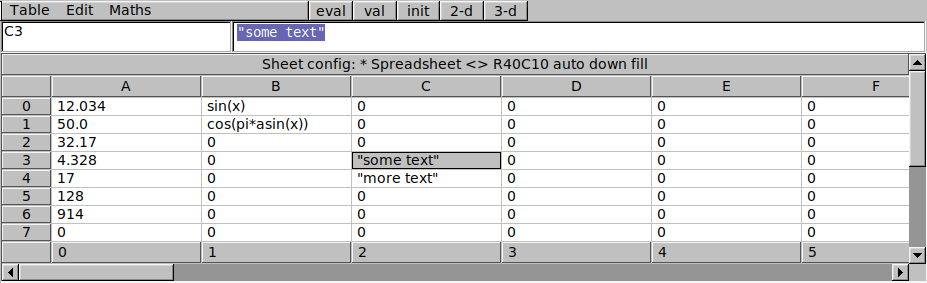
\includegraphics[width=\linewidth]{xcas-spreadsheet.png}
  \caption{\label{fig:spreadsheet}A spreadsheet in \xcas{}}
\end{figure}
When you open a spreadsheet, the input line will become the
spreadsheet, like the one shown in Figure~\ref{fig:spreadsheet}.
The top will be a menu bar with
\textsf{Table}, \textsf{Edit} and \textsf{Maths} menus as well as
\button{eval}, \button{val}, \button{init}, \button{2D} and \button{3D} buttons.
To the right will be the name of the file the spreadsheet will be
saved into. Below the menu bar will be two boxes; a box which displays
the active cell (and can be used to choose a cell) and a command line
to enter information into the cell. Below that will be a status line,
which can be clicked to return to the configuration screen.

\chapter{CAS building blocks\label{chap:casbb}}

\section{Constants}

\subsection{Numbers\label{sec:numbs}}

\xcas{} works with both real and complex numbers.  The real
numbers can be integers, rational numbers, floating point numbers or
symbolic constants.

You can enter an integer by simply typing the digits.
\begin{xcasinput}
1234321
\end{xcasinput}
\begin{xcasoutput}
  1234321
\end{xcasoutput}
Alternatively, you can enter an integer in binary (base 2) by
prefixing the digits (0 through 1) with \texttt{0b}, in octal (base 8)
by prefixing the digits (0 through 7) with \texttt{0} or \texttt{0o},
and in hexadecimal (base 16) by prefixing the digits (0 through 9 and
a through f) with \texttt{0x}.  (See \secref{ssec:binocthex}.)
\begin{xcasinput}
0xab12
\end{xcasinput}
\begin{xcasoutput}
  43794
\end{xcasoutput}

You can enter a rational number as the ratio of two integers.
\begin{xcasinput}
123/45
\end{xcasinput}
\begin{xcasoutput}
  \frac{41}{15}
\end{xcasoutput}
The result will be put in lowest terms.  If the top is a multiple of
the bottom, the result will be an integer.
\begin{xcasinput}
123/3
\end{xcasinput}
\begin{xcasoutput}
  41
\end{xcasoutput}

A floating point number is regarded as an approximation to a real
number.  You can enter a floating point number by writing it out with
a decimal point.
\begin{xcasinput}
123.45
\end{xcasinput}
\begin{xcasoutput}
  123.45
\end{xcasoutput}
You can also enter a floating point number by
entering a sequence of digits, with an optional decimal point,
followed by \texttt{e} and then an integer, where the \texttt{e}
represents ``times 10 to the following power.''
\begin{xcasinput}
1234e3
\end{xcasinput}
\begin{xcasoutput}
  1234000.0
\end{xcasoutput}
Floating point numbers with a large number of digits will be printed with
\texttt{e} notation; you can control how other floats are displayed
(see \secref{ssec:confcomp}, item \ref{enum:float}).
An integer or rational number can be converted to a floating point
number with \texttt{evalf} (see \secref{ssec:evalf}).

A complex number is a number of the form \texttt{$a$+$b$i}, where $a$
and $b$ are real numbers.  The numbers $a$ and $b$ will be the same
type of real number; one type will be converted to the other type if
necessary (an integer can be converted to a rational number or a
floating point number, and a rational number can be converted to a
floating point number).
\begin{xcasinput}
3+1.1i
\end{xcasinput}
\begin{xcasoutput}
  3+1.1\mathrm{i}
\end{xcasoutput}

\subsection{Symbolic constants\label{sec:symbcst}}

Standard constants in \xcas{} are built-in symbols,
given in Table~\ref{tab:symb-constants}\begin{latexonly}, p.~\pageref{tab:symb-constants}\end{latexonly}.
\begin{table}
  \centering
  \begin{tabular}{ll}
    \toprule
    \textbf{Symbol} & \textbf{Value}\\
    \midrule
    \texttt{e}\index{e@\texttt{e}} (or \texttt{\%e}\index{\%e@\texttt{\%e}}) &
                                                                               the number $ \mathrm{e}^{1}$\\
    \texttt{pi}\index{pi@\texttt{pi}} (or \texttt{\%pi}\index{\%pi@\texttt{\%pi}}) &
                                                                                     the number $\pi$\\
    \texttt{infinity}\index{infinity@\texttt{infinity}} & unsigned $\infty$\\
    \texttt{+infinity}\index{+infinity@\texttt{+infinity}} (or \texttt{inf}\index{inf@\texttt{inf}}) &
                                                                                                       $+\infty$\\
    \texttt{-infinity}\index{-infinity@\texttt{-infinity}} (or \texttt{-inf}\index{-inf@\texttt{-inf}}) &
                                                                                                          $-\infty$\\
    \texttt{i}\index{i@\texttt{i}} (or \texttt{\%i}\index{\%i@\texttt{\%i}}) &
                                                                               the complex number $0+1\cdot\mathrm{i}$\\
    \texttt{euler\_gamma}\index{euler\_gamma@\texttt{euler\_gamma}} &
                                                                      Euler's constant $\gamma:=\lim_{n\to\infty}\left(\sum_{k=1}^{n}\frac{1}{k}-\ln(n)\right)$\\
    \bottomrule
  \end{tabular}
  \caption{\label{tab:symb-constants}Symbolic constants in \xcas{}}
\end{table}

Since these numbers cannot be written exactly as standard decimal
numbers, they are necessarily left unevaluated in exact results (see
\secref{ssec:approx}).
\begin{xcasinput}
2*pi
\end{xcasinput}
\begin{xcasoutput}
  2\pi
\end{xcasoutput}
\begin{xcasinput}
2.0*pi
\end{xcasinput}
\begin{xcasoutput}
  6.28318530718
\end{xcasoutput}
You can also use \texttt{evalf} (see \secref{ssec:evalf}), for
example, to approximate one of the real-valued constants to as many
decimal places as you want.
\begin{xcasinput}
evalf(pi,50)
\end{xcasinput}
\begin{xcasoutput}
  3.1415926535897932384626433832795028841971693993751
\end{xcasoutput}

\section{Sequences, sets and lists\label{sec:seqlst}}

\subsection{Sequences\label{ssec:seqbasics}}

A sequence is represented by a sequence of elements separated by
commas, without delimiters or with either parentheses (\texttt{(} and
\texttt{)})\index{()@\texttt{()}} or \texttt{seq[} and
\texttt{]}\index{seq[]@\texttt{seq[]}} as delimiters, as in:
\begin{xcasinput}
1,2,3,4
\end{xcasinput}
or:
\begin{xcasinput}
(1,2,3,4)
\end{xcasinput}
or:
\begin{xcasinput}
seq[1,2,3,4]
\end{xcasinput}
\begin{xcasoutput}
  1,2,3,4
\end{xcasoutput}

Note that the order of the elements of a sequence is significant. For
example, if \texttt{B:=(5,6,3,4)} and \texttt{C:=(3,4,5,6)}, then
\texttt{B==C} returns \texttt{false}.

(A value can be assigned to a variable with the \texttt{:=} operator;
see \secref{ssec:varname}.
Also, \texttt{==} is the test for equality; see
\secref{ssec:booltests}.)

Note also that the expressions \texttt{seq[$\ldots$]} and
\texttt{seq($\ldots$)} are not the same (see \secref{ssec:makeseq} for
information on \texttt{seq($\ldots$)}). For example,
\texttt{seq([0,2])=(0,0)} and \texttt{seq([0,1,1,5])=[0,0,0,0,0]}
but\\
\texttt{seq[0,2]=(0,2)} and \texttt{seq[0,1,1,5]=(0,1,1,5)}

See \secref{sec:seq} for operations on sequences.

\subsection{Sets\label{ssec:sets}}

To define a set of elements, put the elements separated by commas,
with delimiters \texttt{\%\{} and
\texttt{\%\}}\index{\%\{ \%\}@\texttt{\%\{ \%\}}}
or \texttt{set[} and \texttt{]}\index{set[]@\texttt{set[]}}.
\begin{xcasinput}
set[1,2,3,4]
\end{xcasinput}
or:
\begin{xcasinput}
\end{xcasinput}
\begin{xcasoutput}
  \leftsetbracket 1,2,3,4\rightsetbracket
\end{xcasoutput}
In the \xcas{} output, the set delimiters are displayed
as $\leftsetbracket$ and $\rightsetbracket$ in order
not to confuse sets with lists (see \secref{ssec:lstbasics}).
For example, \leftsetbracket 1,2,3 \rightsetbracket is the set \texttt{\%\{1,2,3\%\}},
unlike [1,2,3] (normal brackets) which is the list \texttt{[1,2,3]}.
\begin{xcasinput}
A:=%{1,2,3,4%}
\end{xcasinput}
or:
\begin{xcasinput}
A:=set[1,2,3,4]
\end{xcasinput}
\begin{xcasoutput}
  \leftsetbracket 1,2,3,4\rightsetbracket
\end{xcasoutput}
\begin{xcasinput}
B:=%{5,5,6,3,4%}
\end{xcasinput}
or:
\begin{xcasinput}
B:=set[5,5,6,3,4]
\end{xcasinput}
\begin{xcasoutput}
  \leftsetbracket 5,6,3,4 \rightsetbracket
\end{xcasoutput}

\paragraph*{Remark.}
The order in a set is not significant and the elements in a set are
all distinct. If you input \texttt{B:=\%\{5,5,6,3,4\%\}} and
\texttt{C:=\%\{3,4,5,3,6\%\}}, then \texttt{B==C} will return \texttt{true}.

See \secref{sec:setops} for operations on sets.

\subsection{Lists\label{ssec:lstbasics}}

A list is delimited by \texttt{[} and \texttt{]}\index{[]@\texttt{[]}}, its
elements must be separated by commas.  For example, \texttt{[1,2,5]}
is a list of three integers.  Lists are also called vectors in
\xcas{}.

Lists can contain lists (for example, a matrix is a list of lists of
the same size, see \secref{sec:defmat}). Lists may be used to
represent vectors (lists of coordinates), matrices, or univariate
polynomials (lists of coefficients by decreasing order, see
\secref{ssec:spoly}).

Lists are different from sequences, because sequences are flat: an
element of a sequence cannot be a sequence. Lists are different from
sets, because for a list, the order is important and the same element
can be repeated in a list (unlike in a set where each element is
unique).  See \secref{sec:lists} for operations on lists.

In \xcas{} output:
\begin{itemize}
\item matrix and list delimiters are displayed as square brackets ($[$ and $]$),
\item polynomial delimiters are displayed as $\leftpolybracket$,
  $\rightpolybracket$
\item set delimiters are displayed as $\leftsetbracket$,
  $\rightsetbracket$.
\end{itemize}

\subsection{Accessing elements\label{ssec:els}}

The elements of sequences and lists are indexed starting from 0 in
\xcas{} syntax mode and from 1 in all other syntax modes (see
\secref{ssec:lang}).  To access an element of a list or a sequence,
follow the list with the index between square brackets\index{[]@\texttt{[]}}.

\subsubsection*{Examples}
\begin{xcasinput}
L:=[2,5,1,4]
\end{xcasinput}
\begin{xcasoutput}
  \left[2,5,1,4\right]
\end{xcasoutput}
\begin{xcasinput}
L[1]
\end{xcasinput}
\begin{xcasoutput}
  5
\end{xcasoutput}
To access the last element of a list or sequence, you can put \texttt{-1} between
square brackets.
\begin{xcasinput}
L[-1]
\end{xcasinput}
\begin{xcasoutput}
  4
\end{xcasoutput}
If you want the indices to start from 1 in \xcas{} syntax mode, you can
enter the index between double brackets.
\begin{xcasinput}
L[[1]]
\end{xcasinput}
\begin{xcasoutput}
  2
\end{xcasoutput}

\section{Variables\label{sec:vars}}

\subsection{Variable names\label{ssec:varname}}

A variable\index{variable} or function name is a sequence of letters,
numbers and underscores that begins with a letter.  If you define your
own variable or function, you cannot use the names of built-in
variables or functions or other keywords reserved by \xcas{}.

\subsection{Assigning values to variables
  \label{ssec:assign}}

You can assign a value to a variable with the
\texttt{:=}\index{:=@\texttt{:=}} operator.
For example, to give the variable \texttt{a} the value of \texttt{4},
enter:
\begin{xcasinput}
a:=4
\end{xcasinput}
Alternatively, use the
\texttt{=>}\index{=>@\texttt{=>}} operator; when
you use this operator, the value comes before the variable:
\begin{xcasinput}
4=>a
\end{xcasinput}
The function \texttt{sto}\index{sto@\texttt{sto}}
(or \texttt{Store}\index{Store@\texttt{Store}})
can also be used; again, the value comes before the variable
(the value is stored into the variable):
\begin{xcasinput}
sto(4,a)
\end{xcasinput}
After any one of these commands, whenever you use the variable
\texttt{a} in an expression, it will be replaced by \texttt{4}.

use sequences or lists to make multiple assignments at the
same time. For example,
\begin{xcasinput}
(a,b,c):=(1,2,3)
\end{xcasinput}
will assign \texttt{a} the value \texttt{1}, \texttt{b} the value
\texttt{2} and \texttt{c} the value \texttt{3}.   Note that this can
be used to swap the values of two variables; with \texttt{a} and
\texttt{b} as above, the command
\begin{xcasinput}
(a,b):=(b,a)
\end{xcasinput}
will set \texttt{a} equal to \texttt{b}'s original value, namely
\texttt{2}, and will set \texttt{b} equal to \texttt{a}'s original
value, namely \texttt{1}.

Another way to assign values to variables, useful in \Maple{} mode, is
with the \texttt{assign}\index{assign@\texttt{assign}} command. If you enter
\begin{xcasinput}
assign(a,3)
\end{xcasinput}
or\index{=@\texttt{=}}
\begin{xcasinput}
assign(a=3)
\end{xcasinput}
then \texttt{a} will have the value \texttt{3}.  You can assign
multiple values at once; if you enter
\begin{xcasinput}
assign([a=1,b=2])
\end{xcasinput}
then \texttt{a} will have the value \texttt{1} and \texttt{b} will
have the value \texttt{2}.  This command can be useful in \Maple{} mode,
where solutions of equations are returned as equations.  For example,
if you enter (in \Maple{} mode):
\begin{xcasinput}
sol:=solve([x+y=1,y=2],[x,y])
\end{xcasinput}
(see \secref{ssec:solve}), you will get
\begin{xcasoutput}
  [x=-1,y=2]
\end{xcasoutput}
If you then enter
\begin{xcasinput}
assign(sol)
\end{xcasinput}
the variable \texttt{x} will have value \texttt{-1} and \texttt{y}
will have the value \texttt{2}.  This same effect can be achieved in
standard \xcas{} mode, where
\begin{xcasinput}
sol:=solve([x+y=1,y=2],[x,y])
\end{xcasinput}
will return
\begin{xcasoutput}
  \left[\left[-1,2\right]\right]
\end{xcasoutput}
In this case, the command
\begin{xcasinput}
[x,y]:=sol[0]
\end{xcasinput}
will assign \texttt{x} the value \texttt{-1} and \texttt{y} the value
\texttt{2}.

\subsection{Assignment by reference
  \label{ssec:refassign}}

A list is simply a sequence of values separated by commas and
delimited by \texttt{[} and \texttt{]} (see \secref{sec:seq}). Suppose
you give the variable \texttt{a} the value \texttt{[1,1,3,4,5]}:
\begin{xcasinput}
a:=[1,1,3,4,5]
\end{xcasinput}
If you later assign to \texttt{a} the value \texttt{[1,2,3,4,5]}, then
a new list is created.  It may be better to just change the second
value in the original list by reference.  This can be done with the
\texttt{=<}\index{=<@\texttt{=<}} command.
Recalling that lists are indexed beginning at 0, the command
\begin{xcasinput}
a[1]=<2
\end{xcasinput}
will simply change the value of the second element of the list instead
of creating a new list, and is a more efficient way to change the
value of \texttt{a} to \texttt{[1,2,3,4,5]}.

\subsection{Copying lists\label{ssec:copy}}

If you enter
\begin{xcasinput}
list1:=[1,2,3]
\end{xcasinput}
and then
\begin{xcasinput}
list2:=list1
\end{xcasinput}
then \texttt{list1} and \texttt{list2} will be equal to the same list,
not simply two lists with the same elements.  In particular, if you
change (by reference) the value of an element of \texttt{list1}, then
the change will also be reflected in \texttt{list2}.  For example, if
you enter
\begin{xcasinput}
list1[1]=<5
\end{xcasinput}
then both \texttt{list1} and \texttt{list2} will be equal to
\texttt{[1,5,3]}.

The \texttt{copy}\index{copy@\texttt{copy}}
command creates a copy of a list (or vector or matrix) which is equal to
the original list, but distinct from it. For example, if you enter
\begin{xcasinput}
list1:=[1,2,3]
\end{xcasinput}
and then
\begin{xcasinput}
list2:=copy(list1)
\end{xcasinput}
then \texttt{list1} and \texttt{list2} will both be \texttt{[1,2,3]},
but now if you enter
\begin{xcasinput}
list1[1]=<5
\end{xcasinput}
then \texttt{list1} will be equal to \texttt{[1,5,3]} but
\texttt{list2} will still be \texttt{[1,2,3]}.

\subsection{Incrementing variables
  \label{ssec:incr}}

You can increase the value of a variable \texttt{a} by \texttt{4}, for
example, with
\begin{xcasinput}
a:=a+4
\end{xcasinput}
If beforehand \texttt{a} were equal to \texttt{4}, it would now be
equal to \texttt{8}.  A shorthand way of doing this is with the
\texttt{+=}\index{+=@\texttt{+=}} operator;
\begin{xcasinput}
a+=4
\end{xcasinput}
will also increase the value of \texttt{a} by \texttt{4}.

Similar shorthands exist for subtraction, multiplication and division.
If \texttt{a} is equal to \texttt{8} and you enter\index{-=@\texttt{-=}}
\begin{xcasinput}
a-=2
\end{xcasinput}
then \texttt{a} will be equal to \texttt{6}.
If you follow this with\index{*=@\texttt{*=}}
\begin{xcasinput}
a*=3
\end{xcasinput}
then \texttt{a} will be equal to \texttt{18},
and finally\index{/=@\texttt{/=}}
\begin{xcasinput}
a/=9
\end{xcasinput}
will end with \texttt{a} equal to \texttt{2}.


\subsection{Storing and recalling variables and their values
  \label{ssec:archiving}}

The \texttt{archive}\index{archive@\texttt{archive}} command stores the
values of variables for later use in a file of your choosing.
\begin{itemize}
\item \texttt{archive} takes two arguments:
  \begin{itemize}
  \item \textit{filename}, a filename in which to store values.
  \item \textit{vars}, a variable or list of variables.
  \end{itemize}
\item \texttt{archive("}\textit{filename}\texttt{",}\textit{vars}\texttt{)}
  saves the values of \textit{vars} (or the values of the variables in
  the list) in file \textit{filename}.
\end{itemize}
For example, if the variable \texttt{a} has the value \texttt{2} and the variable
\texttt{bee} has the value \texttt{"letter"} (a string), then entering
\begin{xcasinput}
archive("foo",[a,bee])
\end{xcasinput}
will create a file named ``\texttt{foo}'' which contains the values
\texttt{2} and \texttt{"letter"} in a format meant to be efficiently
read by \xcas{}.

The \texttt{unarchive}\index{unarchive@\texttt{unarchive}}
command will read the values from a file
created with \texttt{archive}.
\begin{itemize}
\item \texttt{unarchive} takes
  \textit{filename}, the filename.
\item \texttt{unarchive("}\textit{filename}\texttt{")} returns the value
  or list of values stored in \textit{filename}.
\end{itemize}

\subsubsection*{Example}
With the file ``\texttt{foo}'' as above:
\begin{xcasinput}
unarchive("foo")
\end{xcasinput}
\begin{xcasoutput}
  \left[2,\text{``letter''}\right]
\end{xcasoutput}
If you want to reassign these values to \texttt{a} and \texttt{bee},
you can enter
\begin{xcasinput}
[a,bee]:=unarchive("foo")
\end{xcasinput}

\subsection{Copying variables
  \label{ssec:copyvar}}

The \texttt{CopyVar}\index{CopyVar@\texttt{CopyVar}} command copies
the contents of one variable into another, without evaluating the contents.
\begin{itemize}
\item
  \texttt{CopyVar} takes two arguments:
  \begin{itemize}
  \item \textit{fromvar}, the name of a variable to copy from.
  \item \textit{tovar}, the name of a variable to copy to.
  \end{itemize}
\item
  \texttt{CopyVar(}$\textit{fromvar},\textit{tovar}$\texttt{)}
  copies the unevaluated contents of \textit{fromvar} into \texttt{tovar}.
\end{itemize}

\subsubsection*{Example}
\begin{xcasinput}
a:=c:;
c:=5:;
CopyVar(a,b);
\end{xcasinput}
\begin{xcasoutput}
  c
\end{xcasoutput}
then:
\begin{xcasinput}
b
\end{xcasinput}
\begin{xcasoutput}
  5
\end{xcasoutput}
Changing the value if \texttt{c} will also change the output of
\texttt{b}, since \texttt{b} contains  \texttt{c}.
\begin{xcasinput}
c:=10:;
b
\end{xcasinput}
\begin{xcasoutput}
  10
\end{xcasoutput}

\subsection{Assumptions on variables
  \label{ssec:about}}

% If \texttt{variable} is a purely symbolic variable (i.e., it does not
% have a value or any assumptions made about it), then:
% \begin{xcasinput}
% abs(variable)
% \end{xcasinput}
% \begin{xcasoutput}
%   \left|\mathrm{variable}\right|
% \end{xcasoutput}
% since \xcas{} does not know what type of value the
% variable is supposed to represent.

The \texttt{assume}\index{assume@\texttt{assume}}
(or \texttt{supposons}\index{supposons@\texttt{supposons}})
command lets you tell \xcas{} some properties of a variable
without giving the variable a specific value.
\begin{itemize}
\item \texttt{assume} (or \texttt{supposons}) takes one mandatory
  argument and one optional argument:
  \begin{itemize}
  \item \textit{assumptions}, statements about a variable (such as
    equalities and inequalities, possibly combined with \texttt{and} and
    \texttt{or}, and domains).
  \item Optionally, \texttt{additionally}, which indicates that the
    assumptions are to be added to previous assumptions, as opposed to
    replace them.
  \end{itemize}
\item \texttt{assume(}$\textit{assumptions}\,\langle,\texttt{additionally}\,\rangle$\texttt{)}
  places the assumptions on the variable.  With no second argument,
  it will remove any previous assumptions.
\end{itemize}

The \texttt{additionally}\index{additionally@\texttt{additionally}}
command can be used to place additional assumptions on a variable.
\begin{itemize}
\item
  \texttt{additionally} takes
  \textit{assumptions} as above.
\item
  \texttt{additionally(}\textit{assumptions}\texttt{)} adds the
  assumptions to a variable without removing assumptions.
\end{itemize}

The \texttt{about}\index{about@\texttt{about}} command
will display the current assumptions about a variable.
(See~\secref{ssec:imageprops} and~\secref{ssec:audioclipprops} for
other uses of \texttt{about}.)
\begin{itemize}
\item
  \texttt{about} takes
  \textit{var}, the name of a variable.
\item
  \texttt{about(}\textit{var}\texttt{)} returns the current assumptions
  on the variable.
\end{itemize}

The \texttt{purge}\index{purge@\texttt{purge}} command will remove all
values and assumptions about a variable.
\begin{itemize}
\item
  \texttt{purge} takes
  \textit{var}, a variable name or a sequence of variable names.
\item
  \texttt{purge(}\textit{var}\texttt{)} removes any assumptions you have
  made about the variable \textit{var} (or about all the variables in
  the sequence).
\end{itemize}


\subsubsection*{Examples}

If you enter
\begin{xcasinput}
assume(variable>0)
\end{xcasinput}
then \xcas{} will assume that \texttt{variable} is a positive real
number, and so
\begin{xcasinput}
abs(variable)
\end{xcasinput}
will be evaluated to
\begin{xcasoutput}
  \mathrm{variable}
\end{xcasoutput}

You can put one or more conditions in the \texttt{assume} command by
combining them with \texttt{and}\index{and@\texttt{and}} and
\texttt{or}\index{or@\texttt{or}}. For example, if you
want the variable \texttt{a} to be in $[2,4) \cup (6,\infty)$, you can
enter
\begin{xcasinput}
assume((a>=2 and a<4) or a>6)
\end{xcasinput}

If a variable has attached assumptions, then making another assumption
with \texttt{assume} will remove the original assumptions.  To add
extra assumptions, you can either use the \texttt{additionally}
command or give \texttt{assume} a second argument of
\texttt{additionally\index{additionally@\texttt{additionally}}}.  If
you assume that $b > 0$ with
\begin{xcasinput}
assume(b>0)
\end{xcasinput}
and you want to add the condition that $b < 1$, you can either enter
\begin{xcasinput}
assume(b<1,additionally)
\end{xcasinput}
or
\begin{xcasinput}
additionally(b<1)
\end{xcasinput}

As well as equalities and inequalities, you can make assumptions about
the domain of a variable.  If you want \texttt{n} to represent an
integer\index{integer@\texttt{integer}}, for example, you can enter
\begin{xcasinput}
assume(n,integer)
\end{xcasinput}
If you want \texttt{n} to be a positive integer, you can add the
condition
\begin{xcasinput}
additionally(n>0)
\end{xcasinput}
You can also assume a variable is in one of the domains
\texttt{real}, \texttt{integer}, \texttt{complex} or
\texttt{rational} (see \secref{ssec:type}).

You can check the assumptions on a variable with the \texttt{about}
command. For the above positive integer \texttt{n},
\begin{xcasinput}
about(n)
\end{xcasinput}
\begin{xcasoutput}
  [\mathrm{integer},[[0,+\infty]],[0]]
\end{xcasoutput}
The first element tells you that \texttt{n} is an integer, the second
element tells you that \texttt{n} is between $0$ and
$+\infty$, and the third element tells you that the value
$0$ is excluded.

If you assume that a variable is equal to a specific value, such as
\begin{xcasinput}
assume(c=2)
\end{xcasinput}
then by default the variable \texttt{c} will remain unevaluated in
later levels.  If you want an expression involving \texttt{c} to be
evaluated, you would need to put the expression inside the
\texttt{evalf\index{evalf@\texttt{evalf}}} command (see \secref{ssec:evalf}).  After
the above assumption on \texttt{c}, if you enter
\begin{xcasinput}
evalf(c^2+3)
\end{xcasinput}
then you will get
\begin{xcasoutput}
  7.0
\end{xcasoutput}
Right below the \texttt{assume(c=2)} command line
there will be a slider; namely arrows pointing left and right with the
value \texttt{2} between them.  These
can be used to change the values of \texttt{c}.  If you click on the
right arrow, the \texttt{assume(c=2)} command will transform to
\begin{xcasinput}
assume(c=[2.2,-10.0,10.0,0.0])
\end{xcasinput}
and the value between the arrows will be \texttt{2.2}.  Also, any
later levels where the variable \texttt{c} is evaluated will be
re-evaluated with the value of \texttt{c} now \texttt{2.2}.  The
output to
\begin{xcasinput}
evalf(c^2+3)
\end{xcasinput}
will become
\begin{xcasoutput}
  7.84
\end{xcasoutput}
The \texttt{-10.0} and \texttt{10.0} in the \texttt{assume} line
represent the smallest and largest values that \texttt{c} can become
using the sliders.  You can set them yourself in the \texttt{assume}
command, as well as the increment that the value will change; if you
want \texttt{c} to start with the value \texttt{5} and vary between
\texttt{2} and \texttt{8} in increments of \texttt{0.05}, then you can
enter
\begin{xcasinput}
assume(c=[5,2,8,0.05])
\end{xcasinput}

Recall the \texttt{purge} command removes assumptions about a
variable.
\begin{xcasinput}
purge(a)
\end{xcasinput}
then \texttt{a} will no longer have any assumptions made about it.
\begin{xcasinput}
purge(a,b)
\end{xcasinput}
then \texttt{a} and \texttt{b} will no longer have any assumptions
made about them.

\subsection{Unassigning variables\label{ssec:VARS}}

\xcas{} has commands that help you keep track of what variables
you are using and resetting them if desired.  The \texttt{VARS}\index{VARS@\texttt{VARS}}
command will list all the variables that you are using, the
\texttt{purge}\index{purge@\texttt{purge}},
\texttt{DelVar}\index{DelVar@\texttt{DelVar}} and
\texttt{del}\index{del@\texttt{del}} commands will delete
selected variables, and the \texttt{rm\_a\_z}\index{rm\_a\_z@\texttt{rm\_a\_z}}
and \texttt{rm\_all\_vars}\index{rm\_all\_vars@\texttt{rm\_all\_vars}}
commands will remove classes of variables. All variables can be removed by using
\texttt{restart}\index{restart@\texttt{restart}}.

\begin{itemize}
\item
  \texttt{VARS} takes no arguments.
\item
  \texttt{VARS()} returns a list of the variables that you have assigned
  values or made assumptions on.
\end{itemize}

The \texttt{purge} command will clear the values and assumptions you
make on variables (see \secref{ssec:about}).  For \TI{}
compatibility there is also \texttt{DelVar}, and for \Python{}
compatibility there is \texttt{del}.
\begin{itemize}
\item
  The \texttt{purge} command takes
  \textit{var}, the name of a variable.
\item
  \texttt{purge(}\textit{var}\texttt{)} clears the variable \textit{var}
  of all values and assumptions.
\end{itemize}

\begin{itemize}
\item
  The \texttt{DelVar} (and \texttt{del}) commands take one argument:
  \textit{var},  the name of a variable.
\item \texttt{Delvar} \textit{var} (or \texttt{del} \textit{var})
  removes the values attached to \textit{var}.  (Note that
  they do not take their argument in parentheses.
\end{itemize}

The \texttt{rm\_all\_vars} and \texttt{restart} commands clear the
values and assumptions you have made on all variables use.
\begin{itemize}
\item \texttt{rm\_all\_vars} takes no arguments.
\item \texttt{rm\_all\_vars()} removes all the values that you have
  attached to variables.
\end{itemize}

\begin{itemize}
\item \texttt{restart} takes no arguments.
\item \texttt{restart} removes all the values that you have
  attached to variables.  (Note that it does not use parentheses.)
\end{itemize}

The \texttt{rm\_a\_z} command clears the values and assumptions on all
variables with single lowercase letter names.
\begin{itemize}
\item \texttt{rm\_a\_z} takes no arguments.
\item \texttt{rm\_a\_z()}  purges all variables whose names are one letter
  and lowercase.
\end{itemize}

\subsubsection*{Examples}
Enter:
\begin{xcasinput}
a:=1; anothervar:=2
\end{xcasinput}
then:
\begin{xcasinput}
VARS()
\end{xcasinput}
\begin{xcasoutput}
  \left[a,\mathrm{anothervar}\right]
\end{xcasoutput}
To clear the variable \texttt{a}:
\begin{xcasinput}
purge(a)
\end{xcasinput}
or (for \TI{} compatibility):
\begin{xcasinput}
DelVar a
\end{xcasinput}
or (for \Python{} compatibility):
\begin{xcasinput}
del a
\end{xcasinput}
If you have variables names \texttt{A,B,a,b,myvar}, then after:
\begin{xcasinput}
rm_a_z()
\end{xcasinput}
you will only have the variables named \texttt{A,B,myvar}.

\subsection{\texttt{CST} variable
  \label{ssec:CST}}

The menu available with the \button{cust} button in the bandeau on the
onscreen keyboard (see \secref{sec:swin}, item \ref{enum:kbd}) is
defined with the \texttt{CST}\index{CST@\texttt{CST}} variable.
It is a list where each list item determines a menu item;
a list item is either a builtin command
name or a list itself consisting of a string to be displayed in the
menu and the input to be entered when the item is selected.

For example, to create a custom defined menu with the builtin function
\texttt{diff}, a user defined function \texttt{foo}, and a menu item
to insert the number $22/7$, enter:
\begin{xcasinput}
CST:=[diff,["foo",foo],["My pi approx",22/7]]
\end{xcasinput}

Note that if the input to be entered is a variable and the variable
has a value when \texttt{CST} is defined, then \texttt{CST} will
contain the value of the variable.  For example,
\begin{xcasinput}
app:=22/7:; CST:=[diff,["foo",foo],["My pi approx",app]]
\end{xcasinput}
will be equivalent to the previous definition of \texttt{CST}.
However, if the variable does not have a value when \texttt{CST} is
defined, for example:
\begin{xcasinput}
CST:=[diff,["foo",foo],["My pi approx",app]]:; app:=22/7
\end{xcasinput}
then \texttt{CST} will behave as the previous values to begin with,
but in this case if the variable \texttt{app} is changed, the
the result of pressing the \button{My pi approx}
button will change also.

Since \texttt{CST} is a list, a function can be added to the
\texttt{cust} menu by using the \texttt{concat} command (see
\secref{ssec:concat}):
\begin{xcasinput}
CST:=concat(CST,evalc)
\end{xcasinput}
will add the \texttt{evalc} command to the \texttt{cust} menu.

\section{Functions}

\subsection{Defining functions\label{ssec:deffuns}}

Similar to how you can assign a value to a variable (see
\secref{ssec:assign}), use the \texttt{:=}\index{:=@\texttt{:=}} and
\texttt{=>}\index{=>@\texttt{=>}} operators to define a function; both
\begin{xcasinput}
f(x):=x^2
\end{xcasinput}
and
\begin{xcasinput}
x^2=>f(x)
\end{xcasinput}
give the name \texttt{f} to the function which takes a value and
returns the square of the value.  In either case, if you then enter:
\begin{xcasinput}
f(3)
\end{xcasinput}
you will get:
\begin{xcasoutput}
  9
\end{xcasoutput}

You can define an anonymous function, namely a function without a
name, with the \texttt{->}\index{->@\texttt{->}} operator;
for example, the squaring function
can be defined by
\begin{xcasinput}
x->x^2
\end{xcasinput}
use this form of the function to assign it a name; both
\begin{xcasinput}
f:=x->x^2
\end{xcasinput}
and
\begin{xcasinput}
x->x^2=>f
\end{xcasinput}
are alternate ways to define \texttt{f} as the squaring function.

You can similarly define functions of more than one variable.  For
example you could enter
\begin{xcasinput}
hypot(a,b):=sqrt(a^2+b^2)
\end{xcasinput}
or
\begin{xcasinput}
hypot:=(a,b)->sqrt(a^2+b^2)
\end{xcasinput}
to define a function which takes the lengths of the two legs
of a right triangle and returns the hypotenuse.

\section{Directories\index{directories}}

\subsection{Working directories
  \label{ssec:wdir}}

\xcas{} has a working directory where it stores files that it
creates; typically this is the user's home directory. The
\texttt{pwd}\index{pwd@\texttt{pwd}}
command will tell you what the current working directory is, and and
the \texttt{cd}\index{cd@\texttt{cd}} command lets you change it.

\begin{itemize}
\item \texttt{pwd} takes no arguments.
\item \texttt{pwd()} returns the name of the current working directory.
\item \texttt{cd} command takes
  \textit{dirname}, the name of a directory (a string).
\item \texttt{cd(}\textit{dirname}\texttt{)} changes the working directory to
  \textit{dirname}.

\end{itemize}

\subsubsection*{Examples}
\begin{xcasinput}
pwd()
\end{xcasinput}
The output might be something like:
\begin{xcasoutput}
  \text{``/home/username''}
\end{xcasoutput}
If you enter:
\begin{xcasinput}
cd("foo")
\end{xcasinput}
or (on a Unix system):
\begin{xcasinput}
cd("/home/username/foo")
\end{xcasinput}
then the working directory will change to the directory \texttt{foo},
if it exists. Afterwards, any files that you save from \xcas{}
will be in that directory.


To load or read a file, it will need to be in the working directory.
Note that if you have the same file name in different directories,
then loading the file name will load the file in the current
directory.

\subsection{Reading files
  \label{ssec:read}}

Information for \xcas{} can be stored in a file; this
information can be read with the
\texttt{read}\index{read@\texttt{read}} or
\texttt{load}\index{load@\texttt{load}}
command, depending on the type of information.

\medskip

The \texttt{read} command reads a file containing \xcas{}
information, such as a program that you saved (see
\secref{ssec:progsave}) or simply commands that you typed into a file
with a text editor.  The file should have the suffix \texttt{.cxx}.
\begin{itemize}
\item
  \texttt{read} takes
  \textit{filename}, the name of a file (a string) containing a saved program (see
  \secref{ssec:progsave}) or other commands.
\item
  \texttt{read(}\textit{filename}\texttt{)} reads the content of
  the file.
\end{itemize}

The \texttt{load} command reads in a saved session (see
\secref{ssec:sesssave}), which will end in \texttt{.xws}.
\begin{itemize}
\item
  \texttt{load} takes
  \textit{filename}, the name of a file (a string) containing a saved session.
\item
  \texttt{load(}\textit{filename}\texttt{)} loads the session stored in
  \textit{filename}.
\end{itemize}

\subsubsection*{Examples}
If you have a file named \texttt{myfunction.cxx},
\begin{xcasinput}
read("myfunction.cxx")
\end{xcasinput}
will read in the file, as long as the directory is in the current working
directory.  If the file is in a different directory, you can still
read it by giving the path to the file,
\begin{xcasinput}
read("/path/to/file/myfunction.cxx")
\end{xcasinput}
If you have a session saved in the file \texttt{mysession.xws},
\begin{xcasinput}
load("mysession.xws")
\end{xcasinput}
loads \texttt{mysession.xws}.

\subsection{Internal directories
  \index{internal directories}}

You can create a directory that isn't actually on your hard drive but
is treated like one by \xcas{} with the command
\texttt{NewFold}\index{NewFold@\texttt{NewFold}}.
\begin{itemize}
\item
  \texttt{NewFold} takes one argument: 
  \textit{MyIntDir}, a variable name (see \secref{ssec:varname}).
\item
  \texttt{NewFold(}\textit{MyIntDir}\textit{)}
  creates a new internal directory named \textit{MyIntDir}.
  (Note that quotation marks are not used.)
\end{itemize}

Internal directories will be listed with the
\texttt{VARS()}\index{VARS@\texttt{VARS}} command
(see \secref{ssec:VARS}).
To actually use this directory, you will have to use the
\texttt{SetFold} command.
\begin{itemize}
\item
  The \texttt{SetFold}\index{SetFold@\texttt{SetFold}} command takes
  \textit{MyIntDir}, the variable name  of an internal directory created with
  \texttt{NewFold}.
\item
  \texttt{SetFold(}\textit{MyIntDir}\texttt{)}
  makes \textit{MyIntDir} the working directory (see \secref{ssec:wdir}).
\end{itemize}

You can print out the internal directory that you are in with
the \texttt{GetFold} command.
\begin{itemize}
\item \texttt{GetFold}\index{GetFold@\texttt{GetFold}} takes no arguments.
\item \texttt{GetFold()} returns the name of the current internal
  directory.
\end{itemize}

The \texttt{DelFold}\index{DelFold@\texttt{DelFold}}
command will delete an internal directory.
\begin{itemize}
\item
  \texttt{DelFold} takes
  \textit{MyIntDir}, the variable name of an internal directory.
\item
  \texttt{DelFold(}\textit{MyIntDir}\texttt{)} will delete the directory
  if it is empty.
\end{itemize}

\chapter{Booleans and strings\label{chap:booleans-strings}}

\section{Booleans\label{sec:boolean}}

\subsection{Boolean values
  \index{boolean}}

The symbols \texttt{true}\index{true@\texttt{true}}
and \texttt{false}\index{false@\texttt{false}} are \textit{booleans},
and are meant to indicate a statement is true or false.

These constants have synonyms:
\begin{itemize}
\item \texttt{true} is the same as
  \texttt{TRUE}\index{TRUE@\texttt{TRUE}}.
\item \texttt{false} is the same as
  \texttt{FALSE}\index{FALSE@\texttt{FALSE}}.
\item \texttt{true} and \texttt{false}
  are both integers with values 1 and 0,
  respectively, but have a different subtype than
  ordinary integers to indicate that they are
  boolean values.
\end{itemize}

A function which returns a boolean is called a \emph{test} (or a
\emph{condition} or a \emph{boolean function}).

\subsection{Comparison operators\label{ssec:booltests}}

The usual comparison operators between numbers are examples of tests.
In \xcas{}, they are the following infixed operators:
\begin{itemize}
\item\index{==@\texttt{==}}
  $a\texttt{==}b$ tests the equality
  between $a$ and $b$ and returns \texttt{1} if $a$
  is equal to $b$ and \texttt{0} otherwise.
\item\index{!=@\texttt{!=}}
  $a\texttt{!=}b$ returns \texttt{1} if $a$ and
  $b$ are different and \texttt{0} otherwise.
\item\index{>=@\texttt{>=}}
  $a\texttt{>=}b$ returns \texttt{1} if $a$
  is greater than or equal to $b$ and \texttt{0} otherwise.
\item\index{>@\texttt{>}}
  $a\texttt{>}b$ returns \texttt{1} if $a$ is strictly
  greater than $b$ and \texttt{0} otherwise.
\item\index{=<@\texttt{=<}}
  $a\texttt{<=}b$ returns \texttt{1} if $a$ is less
  than or equal to $b$ and  \texttt{0} otherwise.
\item\index{<@\texttt{<}}
  $a\texttt{<}b$ returns \texttt{1} if $a$
  is strictly less than $b$ and \texttt{0} otherwise.
\end{itemize}

\paragraph*{Remark.}
Note that \texttt{$a$=$b$} is \textbf{not} a boolean. This form is
used to state that the expression \emph{is} an equality, perhaps with the
intent to solve it.  To test for equality, you need to use
\texttt{$a$==$b$}, which \emph{is} a boolean.

\subsection{Defining functions with boolean tests
  \label{ssec:piecewise}}
\index{piecewise defined functions}

use boolean tests to define functions not given by a single
simple formula.  Notably, use the \texttt{ifte} command or the
\texttt{?:} operator to define piecewise-defined functions.
\begin{itemize}
\item \texttt{ifte}\index{ifte@\texttt{ifte}} takes three arguments:
  \begin{itemize}
  \item \textit{condition}, a boolean condition.
  \item \textit{restrue}, the result to return if
    \textit{condition} is true.
  \item \textit{resfalse}, the result to return if
    \textit{condition} is false.
  \end{itemize}
\item \texttt{ifte(}$\textit{condition},\textit{restrue},\textit{resfalse}$\texttt{)}
  returns \textit{restrue} if
  \textit{condition} holds and \textit{resfalse} otherwise.
\end{itemize}

\subsubsection*{Example}
You can define your own absolute value function with:
\begin{xcasinput}
myabs(x):=ifte(x>=0,x,-x)
\end{xcasinput}
Hence:
\begin{xcasinput}
myabs(-4)
\end{xcasinput}
\begin{xcasoutput}
  4
\end{xcasoutput}
However, \texttt{myabs} will return an error if it cannot evaluate the
condition.
\begin{xcasinput}
myabs(x)
\end{xcasinput}
\begin{xcasoutput}
  \text{Ifte:~Unable to check test Error:~Bad Argument Value}
\end{xcasoutput}

The \texttt{?:}\index{?:@\texttt{?:}} construct behaves
similarly to \texttt{ifte}, but is structured differently and
does not return an error if the condition cannot be evaluated.
\begin{itemize}
\item The \texttt{?:} construct takes three arguments:
  \begin{itemize}
  \item \textit{condition}, a boolean condition.
  \item \textit{restrue}, the result to return if
    \textit{condition} is true.
  \item \textit{resfalse}, the result to return if
    \textit{condition} is false.
  \end{itemize}
\item
  \textit{condition}\texttt{?}\textit{restrue}\texttt{:}\textit{resfalse}
  returns \textit{restrue} if \textit{condition} holds and
  \textit{resfalse} otherwise.
\end{itemize}

\subsubsection*{Example}
You can define your absolute value function with
\begin{xcasinput}
myabs(x):=(x>=0)?x:-x
\end{xcasinput}
If you enter
\begin{xcasinput}
myabs(-4)
\end{xcasinput}
you will again get
\begin{xcasoutput}
  4
\end{xcasoutput}
but now if the conditional cannot be evaluated, you won't get an error.
\begin{xcasinput}
myabs(x)
\end{xcasinput}
\begin{xcasoutput}
  x\geq 0\;?\;x\;:\;-x
\end{xcasoutput}

The \texttt{when\index{when@\texttt{when}}} and
\texttt{IFTE\index{IFTE@\texttt{IFTE}}} commands
are prefixed synonyms for the \texttt{?:} construct.
\begin{itemize}
\item \texttt{when} (and \texttt{IFTE}) take three arguments:
  \begin{itemize}
  \item \textit{condition}, a boolean condition.
  \item \textit{restrue}, the result to return if
    \textit{condition} is true.
  \item \textit{resfalse}, the result to return if
    \textit{condition} is false.
  \end{itemize}
\item \texttt{when(}$\textit{condition},\textit{restrue},\textit{resfalse}$\texttt{)} and
  \texttt{IFTE(}$\textit{condition},\textit{restrue},\textit{resfalse}$\texttt{)} both
  return \textit{restrue} if \textit{condition} holds and \textit{resfalse} otherwise.
\end{itemize}
\begin{center}
  \texttt{(}\textit{condition}\texttt{)} \texttt{?} \textit{restrue} \texttt{:} \textit{resfalse}
\end{center}
\begin{center}
  \texttt{when(}$\textit{condition},\textit{restrue},\textit{resfalse}$\texttt{)}
\end{center}
and
\begin{center}
  \texttt{IFTE(}$\textit{condition},\textit{restrue},\textit{resfalse}$\texttt{)}
\end{center}
all represent the same expression.

If you want to define a function with several pieces, it may be
simpler to use the \texttt{piecewise\index{piecewise@\texttt{piecewise}}} function.
The latter can also be used for finding piecewise representations of expressions.
\begin{itemize}
\item \texttt{piecewise} can take an even number of
  arguments, followed by a single optional argument:
  \begin{itemize}
  \item \textit{cond$_{1}$, return$_{1}$,
      cond$_{2}$, return$_{2}$, \ldots, cond$_{n}$,
      return$_{n}$}, an arbitrary number of pairs
    of conditions and corresponding return values.
  \item Optionally, \textit{expr}, an expression.
  \end{itemize}
  Alternatively, \texttt{piecewise} can take one argument, an expression \textit{expr}, optionally
  followed by a second argument $x$, an identifier.
  \item With conditional arguments,
  \texttt{piecewise(}$\textit{cond}_{1},\textit{return}_{1},\dots,\textit{cond}_{n},\textit{return}_{n}\,\langle,\textit{expr}\,\rangle$\texttt{)}
  returns an expression which evaluates to \textit{return$_{k}$} if \textit{cond$_{k}$}
  is the first true condition, or to \textit{expr} if none of the conditions are true.
  If \textit{expr} is not given, then the default value is \texttt{undef}.
  \item With a single argument, \texttt{piecewise(}\textit{expr}\texttt{)}
  returns a piecewise representation of \textit{expr}. This is useful if \textit{expr} involves
  Heaviside/signum/absolute value functions, since \texttt{piecewise} attempts to remove them;
  if it fails, then \textit{expr} is returned. The optional second argument
  may be given, specifying the relevant variable (otherwise it is guessed).
\end{itemize}

\subsubsection*{Examples}
To define
\[
  f(x)=
  \begin{cases}
    -2 & \text{if } x < -2\\
    3x+4 & \text{if } -2 \le x < -1\\
    1 & \text{if } -1 \le x < 0\\
    x+1 & \text{if } x \ge 0
  \end{cases}
\]
enter:
\begin{xcasinput}
f(x):=piecewise(x<-2,-2,x<-1,3*x+4,x<0,1,x+1)
\end{xcasinput}
To verify, plot $f(x)$ for e.g.~$-3\leq x\leq 1$.

To convert the expression
$x \operatorname{\theta}\left(x+1\right)-x^{2} \operatorname{\theta}\left(x-1\right)+x^{3} \mathrm{sign}\left(x\right)$ to a piecewise expression, enter:
\begin{xcasinput}
f:=x*Heaviside(x+1)-x^2*Heaviside(x-1)+x^3*sign(x):;
\end{xcasinput}
and then
\begin{xcasinput}
piecewise(f)
\end{xcasinput}
or:
\begin{xcasinput}
piecewise(f,x)
\end{xcasinput}
\begin{xcasoutput}
  \begin{cases}-x^{3},&-1>x\\-x^{3}+x,&0>x\\x^{3}+x,&1>x\\x^{3}-x^{2}+x,&\text{otherwise}\end{cases}
\end{xcasoutput}

\texttt{piecewise} can be used for ``flattening'' expressions containing piecewise
defined subexpressions. For example:
\begin{xcasinput}
piecewise(1+piecewise(x<0,-x,x<1,x,1)*when(x<1/2,4x^2,2-2x),x)
\end{xcasinput}
\begin{xcasoutput}
  \begin{cases}-4 x^{3}+1,&0>x\\4 x^{3}+1,&\frac{1}{2}>x\\-2 x^{2}+2 x+1,&1>x\\-2 x+3,&\text{otherwise}\end{cases}
\end{xcasoutput}

\subsection{Logical operators\label{ssec:bool}}

Booleans can be combined to form new booleans.  For example with
\texttt{and}, the statement ``\textit{bool1} \texttt{and}
\textit{bool2}'' is true if both \textit{bool1} and
\textit{bool2} are true, otherwise the statement is false.

\xcas{} has the standard boolean operators, as follows ($a$ and
$b$ are two booleans):
\begin{itemize}
\item\texttt{or} or \texttt{\mybigparallel} ---
  \index{or@\texttt{or}}\index{\mybigparallel}
  These are infixed operators.
  \texttt{($a$ or $b$)} (or \texttt{($a$ \mybigparallel{}
    $b$)}) returns \texttt{0} (or \texttt{false}) if $a$
  and $b$ are both equal to 0 (or \texttt{false}) and returns
  \texttt{1} (or \texttt{true}) otherwise.
\item\texttt{xor}\index{xor@\texttt{xor}} ---
  This is an infixed operator.  It is the ``exclusive or''
  operator, meaning ``one or the other but not both''.
  \texttt{($a$ xor $b$)} returns \texttt{1} if $a$
  is equal to 1 and $b$ is equal to 0 or if $a$ is equal
  to 0 and $b$ is equal to 1, and returns 0 if $a$ and
  $b$ are both equal to 0 or if $a$ and $b$ are
  both equal to 1.
\item\texttt{and} or \texttt{\&\&} ---
  \index{and@\texttt{and}}\index{\&\&@\texttt{\&\&}}
  These are infixed operators.
  \texttt{($a$ and $b$)} (or \texttt{($a$ \&\&
    $b$)}) returns \texttt{1} (or \texttt{true}) if $a$
  and $b$ are both equal to 1 (or \texttt{true}) and returns
  \texttt{0} (or \texttt{false}) otherwise.
\item\texttt{not}\index{not@\texttt{not}} ---
  This is a prefixed operator.
  \texttt{not($a$)} returns \texttt{1} (or \texttt{true}) if $a$
  is equal to 0 (or \texttt{false}), and \texttt{0} (or
  \texttt{false}) if $a$ is equal to 1 (or \texttt{true}).
\end{itemize}

\subsubsection*{Examples}
\begin{xcasinput}
1>=0 or 1<0
\end{xcasinput}
\begin{xcasoutput}
  1
\end{xcasoutput}
\begin{xcasinput}
1>=0 xor 1>0
\end{xcasinput}
\begin{xcasoutput}
  0
\end{xcasoutput}
\begin{xcasinput}
1>=0 and 1>0
\end{xcasinput}
\begin{xcasoutput}
  1
\end{xcasoutput}
\begin{xcasinput}
not(0==0)
\end{xcasinput}
\begin{xcasoutput}
  0
\end{xcasoutput}

\subsection{Transforming a boolean expression to a list}

The \texttt{exp2list}\index{exp2list@\texttt{exp2list}}
command can transform certain booleans into a list.
\begin{itemize}
\item
  \texttt{exp2list} takes one argument: 
  \textit{eqseq}, a sequence of equalities (or inequalities)
  connected with \texttt{or}s, such as
  \texttt{($x=a_{1}$)~or~\ldots~or~($x=a_{n}$)}.
\item
  \texttt{exp2list(}\textit{eqseq}\texttt{)} returns the list
  $[a_{1},\dots,a_{n}]$ of right-hand sides of the (in)equalities.
\end{itemize}

The \texttt{exp2list} command is useful in \TI{} mode for easier processing
of the answer to a \texttt{solve} command.

\subsubsection*{Examples}
\begin{xcasinput}
exp2list((x=2) or (x=0))
\end{xcasinput}
\begin{xcasoutput}
  \left[2,0\right]
\end{xcasoutput}
\begin{xcasinput}
exp2list((x>0) or (x<2))
\end{xcasinput}
\begin{xcasoutput}
  \left[0,2\right]
\end{xcasoutput}
In \TI{} mode:
\begin{xcasinput}
exp2list(solve((x-1)*(x-2)))
\end{xcasinput}
\begin{xcasoutput}
  \left[1,2\right]
\end{xcasoutput}

\subsection{Transforming a list into a boolean expression}

The \texttt{list2exp}\index{list2exp@\texttt{list2exp}}
command is the inverse of \texttt{exp2list}; it takes lists and
tranforms them into boolean expressions.  It can do this in two ways.
\begin{itemize}
\item \texttt{list2exp} can take two arguments:
  \begin{itemize}
  \item $L$, a list  of values of
    the form $[a_{1},\ldots,a_{n}]$.
  \item $x$, a variable name.
  \end{itemize}
\item
  \texttt{list2exp($L,x$)} returns
  the boolean expression  \texttt{($x=a_{1})$~or~\ldots~or~($x=a_{n}$)}.
\item Alternatively,
  \texttt{list2exp} can take two arguments:
  \begin{itemize}
  \item
    \textit{L}, a list where each element of \textit{L} it itself a list
    of $n$ values of the form $[a_{1},\dots,a_{n}]$.
  \item \textit{vars}, a list $[x_{1},\dots,x_{n}]$ of $n$ variable names.
  \end{itemize}
\item
  \texttt{list2exp(}$\textit{L},\textit{vars}$\texttt{)} returns a
  boolean expression of the form
  \texttt{$(x_{1}=a_{1})$~and~\ldots~and~$(x_{n}=a_{n})$}  for each
  list of $n$ values in the first argument, combined with \texttt{or}s.
\end{itemize}

\subsubsection*{Examples}
\begin{xcasinput}
list2exp([0,1,2],a)
\end{xcasinput}
\begin{xcasoutput}
  a=0\vee a=1\vee a=2
\end{xcasoutput}
\begin{xcasinput}
list2exp(solve(x^2-1=0,x),x)
\end{xcasinput}
\begin{xcasoutput}
  x=-1\vee x=1
\end{xcasoutput}
\begin{xcasinput}
list2exp([[3,9],[-1,1]],[x,y])
\end{xcasinput}
\begin{xcasoutput}
  x=3\wedge y=9\vee x=-1\wedge y=1
\end{xcasoutput}

\subsection{Evaluating booleans}

The \Maple{} command \texttt{evalb}\index{evalb@\texttt{evalb}}
evaluates a boolean expression (see \secref{sec:boolean}).
Since \xcas{} evaluates booleans automatically, it
includes a \texttt{evalb} command only here for compatibility
and is equivalent to \texttt{eval} (see \secref{ssec:eval}).
\begin{itemize}
\item \texttt{evalb} takes
  \textit{bool}, a boolean expression.
\item \texttt{evalb(}\textit{bool}\texttt{)} returns 1 if
  \textit{bool} is true and returns 0 otherwise.
\end{itemize}

\subsubsection*{Examples}
\begin{xcasinput}
evalb(sqrt(2)>1.41)
\end{xcasinput}
or:
\begin{xcasinput}
sqrt(2)>1.41
\end{xcasinput}
\begin{xcasoutput}
  1
\end{xcasoutput}
\begin{xcasinput}
evalb(sqrt(2)>1.42)
\end{xcasinput}
or:
\begin{xcasinput}
sqrt(2)>1.42
\end{xcasinput}
\begin{xcasoutput}
  0
\end{xcasoutput}

\section{Strings}

\subsection{Characters and strings}

Strings are delimited with quotation marks
(\texttt{"})\index{\symbol{34}@\texttt{\symbol{34}}}.
A character is a string of length one.

Do not confuse \texttt{"} with \texttt{'} which is used to prevent evaluation
of an expression (see \secref{ssec:qt}). For example, \texttt{"a"}
returns a string with one character but \texttt{'a'} or
\texttt{quote(a)}\index{quote@\texttt{quote}}
returns the variable \texttt{a} unevaluated.

When a string is entered on a command line, it is evaluated to itself,
hence the output is the same string. You can use \texttt{+} to
concatenate two strings or a string and another object (where the
other object will be converted to a string, see
\secref{ssec:plusconcat}).

\subsubsection*{Examples}
\begin{xcasinput}
"Hello"
\end{xcasinput}
\begin{xcasoutput}
  \text{``Hello''}
\end{xcasoutput}
\begin{xcasinput}
"Hello"+", how are you?"
\end{xcasinput}
\begin{xcasoutput}
  \text{``Hello, how are you?''}
\end{xcasoutput}
\begin{xcasinput}
"Hello"+ 123
\end{xcasinput}
\begin{xcasoutput}
  \text{``Hello123''}
\end{xcasoutput}

You can refer to a particular character of a string using index
notation, like for lists (see \secref{sec:lists}). Indices begin at 0
in \xcas{} mode, 1 in other modes.

\subsubsection*{Example}
\begin{xcasinput}
"Hello"[1]
\end{xcasinput}
\begin{xcasoutput}
  \text{``e''}
\end{xcasoutput}

\subsection{Newline character}

A newline can be inserted into a string with
\texttt{\symbol{92}n}\index{\symbol{92}n@\texttt{\symbol{92}n}}.

\subsubsection*{Example}
\begin{xcasinput}
"Hello\nHow are you?"
\end{xcasinput}
\begin{xcasoutput}
  &\text{``Hello}\\
  &\text{How are you?''}
\end{xcasoutput}

\subsection{Length of a string}

The \texttt{size}\index{size@\texttt{size}}
or \texttt{length}\index{length@\texttt{length}} command finds
the length of a string (as well as the length of lists in
general, see \secref{ssec:listlen}).
\begin{itemize}
\item
  \texttt{size} takes
  \textit{str}, a string.
\item
  \texttt{size(}\textit{str}\texttt{)}
  returns the length of the string.
\end{itemize}

\subsubsection*{Example}
\begin{xcasinput}
size("hello")
\end{xcasinput}
\begin{xcasoutput}
  5
\end{xcasoutput}

\subsection{Extracting portions of a string
  \label{ssec:lrstring}}

The \texttt{left}\index{left@\texttt{left}} and
\texttt{right}\index{right@\texttt{right}} commands find the left
and right parts of a string.  (See \secref{ssec:op}, \secref{ssec:range},
\secref{ssec:lrinterval}, \secref{ssec:lrlist}, \secref{ssec:lhs},
\secref{ssec:rhs}, \secref{ssec:channeldata} and \secref{ssec:setchndata}
for other uses of \texttt{left} and \texttt{right}.)
\begin{itemize}
\item \texttt{left} takes two arguments:
  \begin{itemize}
  \item \textit{str}, a string.
  \item $n$, a non-negative integer.
  \end{itemize}
\item \texttt{left(}$\textit{str},n$\texttt{)} returns the first $n$
  characters of the string \textit{str}.
\item \texttt{right} takes two arguments:
  \begin{itemize}
  \item \textit{str}, a string.
  \item $n$, a non-negative integer.
  \end{itemize}
\item \texttt{right(}$\textit{str},n$\texttt{)} returns the last $n$
  characters of the string \textit{str}.
\end{itemize}

The \texttt{head}\index{head@\texttt{head}}
command finds the first character of a string.
\begin{itemize}
\item \texttt{head} takes
  \textit{str}, a string.
\item \texttt{head(}\textit{str}\texttt{)} returns the first
  character of the string \textit{str}.
\end{itemize}

The \texttt{mid}\index{mid@\texttt{mid}}
command finds a selected part from the middle of a
string.
\begin{itemize}
\item \texttt{mid} takes three arguments:
  \begin{itemize}
  \item \textit{str}, a string.
  \item $p$, an integer for the starting index of the result.
  \item $q$, an integer $q$ for the length of the string.
  \end{itemize}
\item \texttt{mid(}$\textit{str},p,q$\texttt{)} returns the part of
  the string \textit{str} starting with the character at index $p$ with length
  $q$.  (Remember that the first index is 0 in \xcas{} mode.)
\end{itemize}

The \texttt{tail}\index{tail@\texttt{tail}}
command removes the first character of a string.
\begin{itemize}
\item \texttt{tail} takes
  \textit{str}, a string.
\item \texttt{tail(}\textit{str}\texttt{)} returns the string
  \textit{str} without its first character.
\end{itemize}

\subsubsection*{Examples}
\begin{xcasinput}
left("hello",3)
\end{xcasinput}
\begin{xcasoutput}
  \text{``hel''}
\end{xcasoutput}
\begin{xcasinput}
right("hello",4)
\end{xcasinput}
\begin{xcasoutput}
  \text{``ello''}
\end{xcasoutput}
\begin{xcasinput}
head("Hello")
\end{xcasinput}
\begin{xcasoutput}
  \text{``H''}
\end{xcasoutput}
\begin{xcasinput}
mid("Hello",1,3)
\end{xcasinput}
\begin{xcasoutput}
  \text{``ell''}
\end{xcasoutput}
\begin{xcasinput}
tail("Hello")
\end{xcasinput}
\begin{xcasoutput}
  \text{``ello''}
\end{xcasoutput}


\subsection{Concatenation of a sequence of words}

The \texttt{cumSum}\index{cumSum@\texttt{cumSum}}
command works on strings like it does on expressions by doing partial
concatenation (see \secref{ssec:cumsum}).
\begin{itemize}
\item
  \texttt{cumSum} takes
  $L$, a list of strings.
\item
  \texttt{cumSum($L$)} returns a sequence of strings where the element
  of index $k$ is the concatenation of the strings in $L$ with indices 0
  to $k$.
\end{itemize}

\subsubsection*{Example}
\begin{xcasinput}
cumSum("Hello, ","is ","that ","you?")
\end{xcasinput}
\begin{xcasoutput}
  \text{``Hello, ''},\text{``Hello, is ''},
  \text{``Hello, is that ''},\text{``Hello, is that you?''}
\end{xcasoutput}

\subsection{\ASCII{} code of a character}

The \texttt{ord}\index{ord@\texttt{ord}}
command finds the \ASCII{} code of a character.
\begin{itemize}
\item  \texttt{ord} takes
  \textit{str}, a string (or a list of strings).
  \texttt{ord(}\textit{str}\texttt{)} returns the \ASCII{} code of the
  first character of \textit{str} (or the list of the \ASCII{} codes of the first
  characters of the elements of the list \textit{str}).
\end{itemize}

\subsubsection*{Example}
\begin{xcasinput}
ord("a")
\end{xcasinput}
\begin{xcasoutput}
  97
\end{xcasoutput}
\begin{xcasinput}
ord("abcd")
\end{xcasinput}
\begin{xcasoutput}
  97
\end{xcasoutput}
\begin{xcasinput}
ord(["abcd","cde"])
\end{xcasinput}
\begin{xcasoutput}
  \left[97,99\right]
\end{xcasoutput}
\begin{xcasinput}
ord(["a","b","c","d"])
\end{xcasinput}
\begin{xcasoutput}
  \left[97,98,99,100\right]
\end{xcasoutput}

\subsection{\ASCII{} code of a string}

The \texttt{asc}\index{asc@\texttt{asc}} command finds the
\ASCII{} codes of all the characters in a string.
\begin{itemize}
\item  \texttt{asc} takes
  \textit{str}, a string.
\item \texttt{asc(}\textit{str}\texttt{)} returns the list of the
  \ASCII{} codes of the characters of $s$.
\end{itemize}

\subsubsection*{Examples}
\begin{xcasinput}
asc("abcd")
\end{xcasinput}
\begin{xcasoutput}
  \left[97,98,99,100\right]
\end{xcasoutput}
\begin{xcasinput}
asc("a")
\end{xcasinput}
\begin{xcasoutput}
  \left[97\right]
\end{xcasoutput}

\subsection{String defined by the \ASCII{} codes of its characters}

The \texttt{char}\index{char@\texttt{char}}
command translates \ASCII{} codes to strings.
\begin{itemize}
\item \texttt{char} takes
  $c$, an integer representing an \ASCII{} code or a list of \ASCII{} codes.
\item \texttt{char($c$)} returns the string whose character has \ASCII{} code
  $c$ or whose characters have \ASCII{} codes the elements of the list $c$.

\end{itemize}

\subsubsection*{Example}
\begin{xcasinput}
char([97,98,99,100])
\end{xcasinput}
\begin{xcasoutput}
  \text{``abcd''}
\end{xcasoutput}
\begin{xcasinput}
char(97)
\end{xcasinput}
\begin{xcasoutput}
  \text{``a''}
\end{xcasoutput}


Note that there are 256 \ASCII{} codes, 0 through 255.  If \texttt{asc}
is given an integer $c$ not in that range, it will use the integer in
that range which equals $c$ modulo 256.
\begin{xcasinput}
char(353)
\end{xcasinput}
\begin{xcasoutput}
  \text{``a''}
\end{xcasoutput}
because $353-256=97$.

\subsection{Finding a character in a string}

The \texttt{inString}\index{inString@\texttt{inString}}
command tests to see if a string contains a
character.
\begin{itemize}
\item  \texttt{inString} takes two arguments:
  \begin{itemize}
  \item \textit{str}, a string.
  \item $c$, a character.
  \end{itemize}
\item \texttt{inString(}\textit{str}\texttt{$,c$)} returns
  the index of its first occurrence of the character $c$ in the string
  \textit{str}, or \texttt{-1} if $c$ does not occur in \textit{str}.
\end{itemize}

\subsubsection*{Examples}
\begin{xcasinput}
inString("abcded","d")
\end{xcasinput}
\begin{xcasoutput}
  3
\end{xcasoutput}
\begin{xcasinput}
inString("abcd","e")
\end{xcasinput}
\begin{xcasoutput}
  -1
\end{xcasoutput}

\subsection{Concatenating objects into a string\label{ssec:catobj}}

The \texttt{cat}\index{cat@\texttt{cat}}
command transforms a sequence of objects into a string.
\begin{itemize}
\item  \texttt{cat} takes
  \textit{seq}, a sequence of objects.
\item  \texttt{cat(}\textit{seq}\texttt{)} returns the concatenation of the string
  representations of these objects as a single string.
\end{itemize}

\subsubsection*{Examples}
\begin{xcasinput}
cat("abcd",3,"d")
\end{xcasinput}
\begin{xcasoutput}
  \text{``abcd3d''}
\end{xcasoutput}
\begin{xcasinput}
c:=5:;
cat("abcd",c,"e")
\end{xcasinput}
\begin{xcasoutput}
  \text{``abcd5e''}
\end{xcasoutput}
\begin{xcasinput}
purge(c);
cat(15,c,3)
\end{xcasinput}
\begin{xcasoutput}
  \text{``15c3''}
\end{xcasoutput}

\subsection{Adding an object to a string\label{ssec:plusconcat}}

The \texttt{'+'}\index{'+'@\texttt{'+'}}
command can be used like \texttt{cat} (see
\secref{ssec:catobj}), and the \texttt{+}\index{+@\texttt{+}}
operator is the infixed version.
(See \secref{sssec:contextplus} for other uses of \texttt{+} and \texttt{'+'}.)
\begin{itemize}
\item \texttt{'+'} takes
  \textit{seq}, a sequence of objects, at least one of which is a string.
\item \texttt{'+'(}\textit{seq}\texttt{)} returns the concatenation of the string
  representations of the objects in \textit{seq}.
\end{itemize}

\paragraph*{Remark.}
Note that \texttt{+} is infixed and \texttt{'+'} is prefixed.

\subsubsection*{Examples}
\begin{xcasinput}
'+'("abcd",3,"d")
\end{xcasinput}
or:
\begin{xcasinput}
"abcd"+3+"d"
\end{xcasinput}
\begin{xcasoutput}
  \text{``abcd3d''}
\end{xcasoutput}
\begin{xcasinput}
c:=5
\end{xcasinput}
then:
\begin{xcasinput}
"abcd"+c+"d"
\end{xcasinput}
or:
\begin{xcasinput}
'+'("abcd",c,"d")
\end{xcasinput}
\begin{xcasoutput}
  \text{``abcd5d''}
\end{xcasoutput}

\subsection{Transforming a real number into a string}

The \texttt{cat}\index{cat@\texttt{cat}}
command (see \secref{ssec:catobj}) can also be used
to transform a real number into a string, as can
\texttt{+}\index{+@\texttt{+}} (see \secref{ssec:plusconcat}).

If \texttt{cat} has a real number as an argument, the result will be a
string.

\subsubsection*{Example}
\begin{xcasinput}
cat(123)
\end{xcasinput}
\begin{xcasoutput}
  \text{``123''}
\end{xcasoutput}


Similarly, if you add a real number to an empty string, the result
will be a string.

\subsubsection*{Example}
\begin{xcasinput}
""+123
\end{xcasinput}
\begin{xcasoutput}
  \text{``123''}
\end{xcasoutput}

\subsection{Transforming a string into a number\label{sec:expr1}}

The \texttt{expr}\index{expr@\texttt{expr}}
command transforms a string representing a valid
\xcas{} statement into the actual statement.
\begin{itemize}
\item  \texttt{expr} takes
  \textit{str}, a string corresponding to an \xcas{} statement.
\item \texttt{expr(}\textit{str}\texttt{)} evaluates the statement.
\end{itemize}

\subsubsection*{Examples}
\begin{xcasinput}
expr("a:=1")
\end{xcasinput}
\begin{xcasoutput}
  1
\end{xcasoutput}
\begin{xcasinput}
a
\end{xcasinput}
\begin{xcasoutput}
  1
\end{xcasoutput}
In particular, \texttt{expr} can transform a string representing a
number into the number (see \secref{sec:numbs}).
\begin{xcasinput}
expr("123")
\end{xcasinput}
\begin{xcasoutput}
  123
\end{xcasoutput}
\begin{xcasinput}
expr("0123")
\end{xcasinput}
\begin{xcasoutput}
  83
\end{xcasoutput}
since \texttt{0123} represents a base 8 integer (see
\secref{ssec:binocthex}) and $1\cdot 8^2+2\cdot 8+3=83$.
\begin{xcasinput}
expr("0x12f")
\end{xcasinput}
\begin{xcasoutput}
  303
\end{xcasoutput}
since \texttt{0x12f} represents a base 16 number and $1\cdot 16^2+2\cdot 16+15=303$.
\begin{xcasinput}
expr("123.4567")
\end{xcasinput}
\begin{xcasoutput}
  123.4567
\end{xcasoutput}
\begin{xcasinput}
expr("123e-5")
\end{xcasinput}
\begin{xcasoutput}
  0.00123
\end{xcasoutput}

\subsection{Levensthein distance\label{sec:levensthein}}
\index{Distance function!Levensthein}

The \texttt{levenshtein}\index{levenshtein@\texttt{levenshtein}}
command computes the Levenshtein distance between two words, which is the
minimum number of single-character edits (insertions, deletions or substitutions)
required to change one word into the other.

\begin{itemize}
\item \texttt{levenshtein} takes two arguments:
  \begin{itemize}
  \item $s_1$, a vector or string.
  \item $s_2$, a vector or string.
  \end{itemize}
\item \texttt{levenshtein(}$s_1,s_2$\texttt{)}
  returns the minimum number $n$ of edits required to transform $s_1$ into $s_2$.
\end{itemize}

\subsubsection*{Example}
\begin{xcasinput}
levenshtein("kitten","sitting")
\end{xcasinput}
\begin{xcasoutput}
  3
\end{xcasoutput}

\subsection{Hamming distance}
\index{Distance function!Hamming}

The \texttt{hamdist}\index{hamdist@\texttt{hamdist}}
command computes the Hamming distance between two sequences of equal lengths,
which is defined to be the number of elements at same positions which do not match.

\begin{itemize}
\item \texttt{hamdist} takes two arguments:
  \begin{itemize}
  \item $s_1$, a vector or string.
  \item $s_2$, a vector or string.
  \end{itemize}
\item \texttt{hamdist(}$s_1,s_2$\texttt{)}
  returns the number $n$ of characters in $s_1$ that are different
  than the corresponding characters in $s_2$.
\end{itemize}

\subsubsection*{Example}
\begin{xcasinput}
hamdist("cats","dogs")
\end{xcasinput}
\begin{xcasoutput}
  3
\end{xcasoutput}

\section{Bitwise operators}

\subsection{Basic operators}

Bitwise operators operate on the base 2 representations of integers,
even if they are not presented in base 2.  For example, the bitwise
\texttt{or} (see \secref{ssec:bool}) operator will take two integers
and and return an integer whose base 2 digits are the logical
\textit{or}s of the corresponding base two digits of the inputs (see
\secref{ssec:bool}).  Thus, to find the bitwise \textit{or} of
\texttt{6} and \texttt{4}, look at their base 2 representations, which
are \texttt{0b110} (the \texttt{0b} prefix indicates that it's in base
2, see \secref{sec:numbs}) and \texttt{0b100}, respectively.  The
logical \textit{or} or their rightmost digits is \texttt{(0 or
  0)}=\texttt{0}. The logical \texttt{or} of their next digits is
\texttt{(1 or 0)}=\texttt{1}, and the logical \texttt{or} of their
remaining digits is \texttt{(1 or 1)}=\texttt{1}.  So the bitwise or of
\texttt{6} and \texttt{4} is \texttt{0b110}, which is \texttt{6}.

To work with bitwise operators, it isn't necessary but it may be
useful to work with integers in a base which is a power of 2. The
integers can be entered in binary (base 2), octal (base 8) or
hexadecimal (base 16) (see \secref{ssec:binocthex}).  To write an
integer in binary, prefix it with \texttt{0b}; to write an integer in
octal, prefix it with \texttt{0} or \texttt{0o}; and to write a
integer in hexadecimal (base 16), prefix it with \texttt{0x}. Integers
may also be output in octal or hexadecimal notation (see
\secref{ssec:confcomp}, item \ref{enum:base}).

There are bitwise versions of the logical operators \texttt{or},
\texttt{xor} and \texttt{and}, called
\texttt{bitor}\index{bitor@\texttt{bitor}},
\texttt{bitxor}\index{bitxor@\texttt{bitxor}} and
\texttt{bitand}\index{bitand@\texttt{bitand}};
they are all prefixed operators which
take two arguments, which are both integers.

\subsubsection*{Examples}

\begin{xcasinput}
bitor(0x12,0x38)
\end{xcasinput}
  or:
\begin{xcasinput}
bitor(18,56)
\end{xcasinput}
\begin{xcasoutput}
  58
\end{xcasoutput}
because
\texttt{18} is written \texttt{0x12} in base 16 or \texttt{0b010010} in base 2 and
\texttt{56} is written \texttt{0x38} in base 16 or \texttt{0b111000} in base 2,
hence \texttt{bitor(18,56)} is \texttt{0b111010} in base 2 and so is equal to 58.
\begin{xcasinput}
bitxor(0x12,0x38)
\end{xcasinput}
  or:
\begin{xcasinput}
bitxor(18,56)
\end{xcasinput}
\begin{xcasoutput}
  42
\end{xcasoutput}
because
\texttt{18} is written \texttt{0x12} in base 16 and \texttt{0b010010} in base 2 and
\texttt{56} is written \texttt{0x38} in base 16 and \texttt{0b111000} in base 2,
\texttt{bitxor(18,56)} is written \texttt{0b101010} in base 2 and so, is equal to 42.
\begin{xcasinput}
bitand(0x12,0x38)
\end{xcasinput}
  or:
\begin{xcasinput}
bitand(18,56)
\end{xcasinput}
\begin{xcasoutput}
  16
\end{xcasoutput}
because
\texttt{18} is written \texttt{0x12} in base 16 and \texttt{0b010010} in base 2 and
\texttt{56} is written \texttt{0x38} in base 16 and \texttt{0b111000} in base 2,
\texttt{bitand(18,56)} is written \texttt{0b010000} in base 2 and so is equal to 16.

\subsection{Bitwise Hamming distance}
\index{Distance function!Bitwise Hamming}

The Hamming distance between two integers is the number of differences
between the bits of the two integers.
The \texttt{hamdist}\index{hamdist@\texttt{hamdist}} command
finds the Hamming distance between two integers.
\begin{itemize}
\item
  \texttt{hamdist} takes two arguments:
  $m$ and $n$, both integers.
\item
  \texttt{hamdist($m,n$)} returns the Hamming distance
  between $m$ and $n$.
\end{itemize}

\subsubsection*{Example}
\begin{xcasinput}
hamdist(0x12,0x38)
\end{xcasinput}
or:
\begin{xcasinput}
hamdist(18,56)
\end{xcasinput}
\begin{xcasoutput}
  3
\end{xcasoutput}
because
\texttt{18} is written \texttt{0x12} in base 16 and \texttt{0b010010} in base 2 and
\texttt{56} is written \texttt{0x38} in base 16 and \texttt{0b111000} in base 2,
hence \texttt{hamdist(18,56)} is equal to $1+0+1+0+1+0=3$.

\section{Writing an integer in a different base\label{sec:dbase}}

\subsection{Writing an integer in base 2, 8 or 16\label{ssec:binocthex}}

Integers are typically entered and displayed in base 10.  You can also
enter an integer in base 2 (binary)\index{binary},
base 8 (octal)\index{octal} or base 16 (hexadecimal)\index{hexadecimal}.
You can enter:
\begin{itemize}
\item a number in base 2 by prefixing it with \texttt{0b}; the
  remaining digits have to be 0 or 1.
\item an octal number by prefixing it with \texttt{0} or
  \texttt{0o}; the remaining digits have to be 0-7 since it is base 8.
\item a hexadecimal number by prefixing it with \texttt{0x};
  the remaining digits have to be 0-9 or
  A-F (where A is 10, B is 11, \ldots, F is 15).
  Non-capital letters a-f are allowed to be used instead.
\end{itemize}

\subsubsection*{Examples}

Since $101$ in binary is the same as $1\cdot 1+0\cdot 2+1\cdot
2^{2}=5$ in decimal:
\begin{xcasinput}
0b101
\end{xcasinput}
\begin{xcasoutput}
  5
\end{xcasoutput}
Since $512$ in base 8 is the same as $2\cdot 1+1\cdot 8+5\cdot
8^{2}=330$ in decimal:
\begin{xcasinput}
0512
\end{xcasinput}
\begin{xcasoutput}
  330
\end{xcasoutput}
Since 2F3 in base 16 is the same as $3\cdot 1+15\cdot 16+2\cdot
16^{2}=755$ in decimal:
\begin{xcasinput}
0x2F3
\end{xcasinput}
\begin{xcasoutput}
  755
\end{xcasoutput}

You can have \xcas{} print integers in octal or hexadecimal, as
well as the default decimal.  To change the base used for display, you
can click on the red CAS status button and choose from the
\textsf{Integer basis} menu (see \secref{ssec:confcomp}, item
\ref{enum:base}).  If you have \xcas{} set to display in
hexadecimal, you will get the following:
\begin{xcasinput}
15
\end{xcasinput}
\begin{xcasoutput}
  0\mathrm{xF}
\end{xcasoutput}
\begin{xcasinput}
0x15
\end{xcasinput}
\begin{xcasoutput}
  0\mathrm{x15}
\end{xcasoutput}

\subsection{Writing an integer in an arbitrary base
  \label{sec:convertbase}}

The \texttt{convert}\index{convert@\texttt{convert}} or
\texttt{convertir}\index{convertir@\texttt{convertir}}
command does various kinds of conversions depending on the option
given as the second argument (see \secref{ssec:convert}). 

One thing that \texttt{convert} can do is to
convert integers to arbitrary bases and back to the default base, both
with the option \texttt{base}\index{base@\textit{base}}.

\paragraph{Conversion from base 10.}
An integer can be converted into a list of digits in base $b$ by
using the \texttt{convert} command.
\begin{itemize}
\item  \texttt{convert} takes three
  arguments:
  \begin{itemize}
  \item $n$, an integer.
  \item \texttt{base}, the symbol verbatim.
  \item $b$, a positive integer, the value of the base.
  \end{itemize}
\item \texttt{convert($n$,base,$b$)} returns the list of
  digits of the integer $n$ when written in base $b$.  The
  list of digits will start with the 1s term, then the
  $b$s term, the $b^{2}$ term, etc.
\end{itemize}

\subsubsection*{Examples}
\begin{xcasinput}
convert(123,base,8)
\end{xcasinput}
\begin{xcasoutput}
  \left[3,7,1\right]
\end{xcasoutput}
To verify, input \texttt{0173} (see \secref{ssec:binocthex}) or
\texttt{horner(revlist([3,7,1]),8)} (see \secref{ssec:horner} and
\secref{ssec:rlst}) or \texttt{convert([3,7,1],base,8)} which all return 123.

The base used for \texttt{convert} can be any integer greater than 1.
For example, input:
\begin{xcasinput}
convert(142,base,12)
\end{xcasinput}
\begin{xcasoutput}
  \left[10,11\right]
\end{xcasoutput}

\paragraph{Conversion from an arbitrary base $b$.}
A number written in base $b$ can be converted into a base 10 integer
by using the \texttt{convert} command.
\begin{itemize}
\item \texttt{convert} takes three arguments:
  \begin{itemize}
  \item $L$, a list of integers representing the digits of the
    integer in base $b$, assumed to go in order of increasing
    significance.
  \item \texttt{base}, the symbol verbatim.
  \item $b$, a positive integer, the value of the base.
  \end{itemize}
\item \texttt{convert($L$,base,$b$)} returns the integer which, in
  base $b$, has the digits given in $L$.
\end{itemize}

\subsubsection*{Examples}
\begin{xcasinput}
convert([3,7,1],base,8)
\end{xcasinput}
\begin{xcasoutput}
  123
\end{xcasoutput}
\begin{xcasinput}
convert([10,11],base,12)
\end{xcasinput}
\begin{xcasoutput}
  142
\end{xcasoutput}

\chapter{Sequences, lists, and sets}

\section{Sequences and lists\label{sec:seq}}

\subsection{Defining a sequence or a list}

Recall (see \secref{ssec:seqbasics}) that a sequence is represented by
a sequence of elements separated by commas, either without delimiters,
with parentheses (\texttt{(} and \texttt{)})\index{()@\texttt{()}}
as delimiters, or with \texttt{seq[} and \texttt{]}\index{seq[]@\texttt{seq[]}}
as delimiters.

\subsubsection*{Examples}
\begin{xcasinput}
a,b,c,d
\end{xcasinput}
or:
\begin{xcasinput}
(a,b,c,d)
\end{xcasinput}
or:
\begin{xcasinput}
seq[a,b,c,d]
\end{xcasinput}
\begin{xcasoutput}
  a,b,c,d
\end{xcasoutput}

Similarly (see \secref{ssec:lstbasics}) a list (or a vector) is
a sequence of elements separated by commas delimited with \texttt{[}
and \texttt{]}.

\subsubsection*{Examples}
\begin{xcasinput}
[1,2,5]
\end{xcasinput}
\begin{xcasoutput}
  \left[1,2,5\right]
\end{xcasoutput}
To create an empty list, input:
\begin{xcasinput}
[]
\end{xcasinput}
\begin{xcasoutput}
  \left[\right]
\end{xcasoutput}

\paragraph*{Remarks.}
Lists have more structure than sequences.  For example, a list can
contain lists (for example, a matrix is a list of lists of the same
size, see \secref{sec:defmat}). Lists may be used to represent vectors
(lists of coordinates), matrices, or univariate polynomials (lists of
coefficients by decreasing order, see \secref{ssec:spoly}).

Sequences, on the other hand, are flat.  An element of a sequence
cannot be a sequence.

See \secref{sec:lists} for some commands only for lists.

\subsection{Making a sequence or a list\label{ssec:makeseq}}

The \texttt{seq}\index{seq@\texttt{seq}} command or
\texttt{\$}\index{\$@\texttt{\$}} operator can create
a sequence or a list.

\begin{itemize}
\item To create a sequence, \texttt{seq} takes three mandatory arguments
  and one optional argument:
  \begin{itemize}
  \item \textit{expr}, an expression depending on a parameter.
  \item $k$, the parameter.
  \item $a$\texttt{..}$b$, a range of values.
    The range can be combined with the parameter into one argument of
    $k=a\texttt{..}b$.
  \item Optionally $p$, a step size (by default 1 or -1, depending
    on whether $b>a$ or $b<a$).  This is only allowed
    if the previous two arguments are combined into one, $k=a\texttt{..}b$
  \end{itemize}
  This is \Maple{}-like syntax.
\item \texttt{seq(}$\textit{expr},k,a\texttt{..}b$\texttt{)} or
  \texttt{seq(}$\textit{expr},k\texttt{=}a\texttt{..}b \,\langle,p\rangle$\texttt{)}
  returns the sequence formed by the values of \texttt{expr}, as $k$
  changes from $a$ to $b$ in steps of $p$.
\end{itemize}


Alternatively, a sequence can be created with the infixed \texttt{\$} operator.
Namely, \textit{expr}\texttt{\$($k$=$a$..$b$)}
returns the sequence formed by the values of \texttt{expr} as $k$
changes from $a$ to $b$.  As a special case, \textit{expr}\texttt{\$$n$}
creates a sequence consisting of $n$ copies of \textit{expr}.

There are two ways to create a list with \texttt{seq}.
\begin{itemize}
\item \texttt{seq} can take four mandatory arguments
  and one optional argument:
  \begin{itemize}
  \item \textit{expr}, an expression depending on a parameter.
  \item $k$, the parameter.
  \item $a$, the beginning value of the parameter.
  \item $b$, the ending value of the parameter.
  \item Optionally $p$, a step size (by default 1 or -1, depending
    on whether $b>a$ or $b<a$).
  \end{itemize}
  This is \TI{}-like syntax.
\item \texttt{seq(}$\textit{expr},k,a,b \,\langle,p\rangle$\texttt{)}
  returns the list consisting of the values of \texttt{expr}, as $k$
  changes from $a$ to $b$ in steps of $p$.
\item As a special case, \texttt{seq(}$\textit{expr},n$\texttt{)}
  creates a list consisting of $n$ copies of \textit{expr}.
\item Alternatively, \texttt{seq} can take two arguments:
  \begin{itemize}
  \item \textit{expr}, an expression.
  \item $n$, a positive integer.
  \end{itemize}
\item \texttt{seq(}$\textit{expr},n$\texttt{)}
  returns the list consisting of $n$ copies of \texttt{expr}.
\end{itemize}

\paragraph*{Remarks.}
In \xcas{} mode, the precedence of \texttt{\$} is not the
same as it is, for example, in \Maple{}.  In case of doubt,
put the arguments of \texttt{\$} in parenthesis.
For example, the following commands are equivalent:
\begin{xcasinput}
seq(j^2,j=-1..3)
\end{xcasinput}
or
\begin{xcasinput}
(j^2)$(j=-1..3)
\end{xcasinput}
\begin{xcasoutput}
  1,0,1,4,9
\end{xcasoutput}

With \Maple{} syntax, \texttt{j,a..b,p} is not valid.
To specify a step $p$ for the variation of
$j$ from $a$ to $b$, use \texttt{j=a..b,p} or use the \TI{} syntax
\texttt{j,a,b,p} and get the sequence from the list with
\texttt{op(\ldots)}.

\subsubsection*{Examples}
To create a sequence:
\begin{xcasinput}
seq(j^3,j,1..4)
\end{xcasinput}
or:
\begin{xcasinput}
seq(j^3,j=1..4)
\end{xcasinput}
or:
\begin{xcasinput}
(j^3)$(j=1..4)
\end{xcasinput}
\begin{xcasoutput}
  1,8,27,64
\end{xcasoutput}
To create a list:
\begin{xcasinput}
seq(j^3,j,1,4)
\end{xcasinput}
\begin{xcasoutput}
  \left[1,8,27,64\right]
\end{xcasoutput}
To create a sequence:
\begin{xcasinput}
seq(j^3,j=-1..4,2)
\end{xcasinput}
\begin{xcasoutput}
  -1,1,27
\end{xcasoutput}
To create a list:
\begin{xcasinput}
seq(j^3,j,-1,4,2)
\end{xcasinput}
\begin{xcasoutput}
  \left[-1,1,27\right]
\end{xcasoutput}
\begin{xcasinput}
seq(j^3,j,0,5,2)
\end{xcasinput}
\begin{xcasoutput}
  \left[0,8,64\right]
\end{xcasoutput}
\begin{xcasinput}
seq(j^3,j,5,0,-2)
\end{xcasinput}
or:
\begin{xcasinput}
seq(j^3,j,5,0,2)
\end{xcasinput}
\begin{xcasoutput}
  \left[125,27,1\right]
\end{xcasoutput}
\begin{xcasinput}
seq(j^3,j,1,3,0.5)
\end{xcasinput}
\begin{xcasoutput}
  \left[1,3.375,8.0,15.625,27.0\right]
\end{xcasoutput}
\begin{xcasinput}
seq(j^3,j,1,3,1/2)
\end{xcasinput}
\begin{xcasoutput}
  \left[1,\frac{27}{8},8,\frac{125}{8},27\right]
\end{xcasoutput}
To create a list with several copies of the same element:
\begin{xcasinput}
seq(t,4)
\end{xcasinput}
\begin{xcasoutput}
  \left[t,t,t,t\right]
\end{xcasoutput}
To create a sequence with several copies of the same element:
\begin{xcasinput}
seq(t,k=1..4)
\end{xcasinput}
or:
\begin{xcasinput}
t$4
\end{xcasinput}
\begin{xcasoutput}
  t,t,t,t
\end{xcasoutput}

\subsubsection*{Examples of sequences being used}
Find the third derivative of $\ln(t)$ (see \secref{ssec:diff}):
\begin{xcasinput}
diff(log(t),t$3)
\end{xcasinput}
\begin{xcasoutput}
  \frac{2}{t^{3}}
\end{xcasoutput}
\begin{xcasinput}
l:=[[2,3],[5,1],[7,2]]
seq((l[k][0])$(l[k][1]),k=0..size(l)-1)
\end{xcasinput}
\begin{xcasoutput}
  \left(2,2,2\right),\left(5\right),\left(7,7\right)
\end{xcasoutput}
then:
\begin{xcasinput}
eval(ans())
\end{xcasinput}
\begin{xcasoutput}
  2,2,2,5,7,7
\end{xcasoutput}
Transform a string into a list of its characters:
\begin{xcasinput}
chn:="abracadbra":;
seq(chn[j],j,0,size(chn)-1)
\end{xcasinput}
\begin{xcasoutput}
  \left[\text{``a''},\text{``b''},\text{``r''},\text{``a''},\text{``c''},
    \text{``a''},\text{``d''},\text{``a''},\text{``b''},\text{``r''},\text{``a''}\right]
\end{xcasoutput}

\subsection{Length of a sequence or list\label{ssec:listlen}}

You can find the length of a sequence or list with any of the
\texttt{size}\index{size@\texttt{size}},
\texttt{nops}\index{nops@\texttt{nops}} or
\texttt{length}\index{length@\texttt{length}} commands.
\begin{itemize}
\item Each of \texttt{size}, \texttt{nops} and \texttt{length} takes
  $S$, a sequence or list.
\item Each of \texttt{size($S$)}, \texttt{nops($S$)} and
  \texttt{length($S$)} returns the length of $L$.
\end{itemize}

\subsubsection*{Examples}
\begin{xcasinput}
nops(a,e,i,o,u)
\end{xcasinput}
or:
\begin{xcasinput}
size(a,e,i,o,u)
\end{xcasinput}
or:
\begin{xcasinput}
length(a,e,i,o,u)
\end{xcasinput}
\begin{xcasoutput}
  5
\end{xcasoutput}
\begin{xcasinput}
nops([3,4,2])
\end{xcasinput}
or:
\begin{xcasinput}
size([3,4,2])
\end{xcasinput}
or:
\begin{xcasinput}
length([3,4,2])
\end{xcasinput}
\begin{xcasoutput}
  3
\end{xcasoutput}

\subsection{Getting the first element of a sequence or list}

The \texttt{head}\index{head@\texttt{head}} command
finds the first element of a sequence or list.
\begin{itemize}
\item \texttt{head} takes
  $S$, a sequence or list.
\item \texttt{head($S$)} returns the first element of $S$.
\end{itemize}

\subsubsection*{Examples}
\begin{xcasinput}
head(A,B,C,D)
\end{xcasinput}
\begin{xcasoutput}
  A
\end{xcasoutput}
\begin{xcasinput}
head([0,1,2,3])
\end{xcasinput}
\begin{xcasoutput}
  0
\end{xcasoutput}

\subsection{Getting a sequence or list without the first element}

The \texttt{tail}\index{tail@\texttt{tail}} command
removes the first element of a list.
\begin{itemize}
\item \texttt{tail} takes
  $L$, a list.
\item \texttt{tail($L$)} returns $L$ without its first element.
\end{itemize}

\subsubsection*{Example}
\begin{xcasinput}
tail([0,1,2,3])
\end{xcasinput}
\begin{xcasoutput}
  \left[1,2,3\right]
\end{xcasoutput}

\subsection{Getting an element of a sequence or a list
  \label{ssec:getels}}

The elements of a sequence have indices beginning at 0 in
\xcas{} mode and 1 in other modes (see \secref{ssec:lang}).

You can get the an element of index $n$ of a sequence or list by following
the sequence or list with $[n]$\index{[]@\texttt{[]}}
(see \secref{ssec:els}).

(Note that \texttt{head($S$)} does the same thing as \texttt{$S$[0]}.)

\subsubsection*{Examples}
\begin{xcasinput}
(0,3,2)[1]
\end{xcasinput}
\begin{xcasoutput}
  3
\end{xcasoutput}
\begin{xcasinput}
S:=2,3,4,5:;
S[2]
\end{xcasinput}
\begin{xcasoutput}
  4
\end{xcasoutput}
\begin{xcasinput}
[A,B,C,D][2]
\end{xcasinput}
\begin{xcasoutput}
  C
\end{xcasoutput}

For lists, the \texttt{at}\index{at@\texttt{at}} command
can also be used to get the element at a specific position.
\begin{itemize}
\item \texttt{at} takes two arguments:
  \begin{itemize}
  \item $L$, a list.
  \item $n$, an integer.
  \end{itemize}
\item \texttt{at($L,n$)} returns the element of $S$ with index $n$.
\end{itemize}
\paragraph{Note.}
\texttt{at} cannot be used for sequences, since the second argument
would be merged with the sequence.

\subsubsection*{Example}
\begin{xcasinput}
[0,1,2][1]
\end{xcasinput}
or:
\begin{xcasinput}
at([0,1,2],1)
\end{xcasinput}
\begin{xcasoutput}
  1
\end{xcasoutput}

\subsection{Finding a subsequence or a sublist}

The bracket notation used to find elements of sequences and lists can
also be used to extract a range of elements.
If $S$ is a sequence or list of size $n$, then
\texttt{$S$[$n_{1}$..$n_{2}$]} returns the subsequence or sublist
of $S$ consisting of the elements with indices from $n_1$ to
$n_2$, where $0 \leq n_1\leq n_2 < s$ (in \xcas{} syntax mode) or $0 <
n_1\leq n_2 \leq s$ in other syntax modes.

For lists, the \texttt{at}\index{at@\texttt{at}}
command can also be used to get a sublist.
\begin{itemize}
\item \texttt{at} takes two arguments:
  \begin{itemize}
  \item $L$, a list.
  \item $n_{1}\texttt{..}n_{2}$, a range of integers.
  \end{itemize}
\item \texttt{at($L,n_{1}$..$n_{2}$)} returns the sublist
  of $L$ consisting of the elements with indices from $n_1$ to
  $n_2$.
\end{itemize}
Again, \texttt{at} cannot be used for sequences.

An alternative to using \texttt{at} for finding a sublist is the
\texttt{mid}\index{mid@\texttt{mid}} command,
which again cannot be used for sequences.
\begin{itemize}
\item \texttt{mid} takes two mandatory and one optional argument:
  \begin{itemize}
  \item $L$, a list.
  \item $n$, the index of the beginning of the sublist.
  \item Optionally, $l$, the length of the sublist.
  \end{itemize}
\item \texttt{mid($L,n \,\langle,l\rangle$)} returns the sublist of $L$ with index
  beginning at $n$.  With the option $l$, the length of the sublist
  will be $l$, otherwise it will go to the end of the list $L$.
\end{itemize}

\subsubsection*{Examples}
\begin{xcasinput}
[0,1,2,3,4][1..3]
\end{xcasinput}
\begin{xcasoutput}
  \left[1,2,3\right]
\end{xcasoutput}
\begin{xcasinput}
(A,B,C,D,E)[1..3]
\end{xcasinput}
\begin{xcasoutput}
  B,C,D
\end{xcasoutput}
\begin{xcasinput}
at([1,2,3,4,5],2..4
\end{xcasinput}
\begin{xcasoutput}
  \left[3,4,5\right]
\end{xcasoutput}
\begin{xcasinput}
mid([0,1,2,3,4,5],2,3)
\end{xcasinput}
\begin{xcasoutput}
  \left[2,3,4\right]
\end{xcasoutput}
\begin{xcasinput}
mid([0,1,2,3,4,5],2)
\end{xcasinput}
\begin{xcasoutput}
  \left[2,3,4,5\right]
\end{xcasoutput}

\subsection{Concatenating sequences}

The \texttt{,}\index{,@\texttt{,}}
operator is an infixed operator which concatenates two sequences.
(Note that it does not concatenate lists.)

\subsubsection*{Example}
\begin{xcasinput}
A:=(1,2,3,4);
B:=(5,6,3,4);
A,B
\end{xcasinput}
\begin{xcasoutput}
  1,2,3,4,5,6,3,4
\end{xcasoutput}

\subsection{The \texttt{+} operator applied on sequences and lists
  \label{ssec:plusseq}}

The infixed operator \texttt{+}\index{+@\texttt{+}},
with two sequences as arguments, returns the total sum of the elements
of the two sequences. This is different than with two lists as arguments,
where the term by term sums of the elements of the two lists would be returned.
(See \secref{sssec:contextplus}.)  To use it as a prefix,
it has to be quoted (\texttt{'+'}).

\subsubsection*{Examples}
\begin{xcasinput}
(1,2,3,4,5,6)+(4,3,5)
\end{xcasinput}
or:
\begin{xcasinput}
'+'((1,2,3,4,5,6),(4,3,5))
\end{xcasinput}
\begin{xcasoutput}
  33
\end{xcasoutput}
\begin{xcasinput}
[1,2,3,4,5,6]+[4,3,5]
\end{xcasinput}
or:
\begin{xcasinput}
'+'([1,2,3,4,5,6],[4,3,5])
\end{xcasinput}
\begin{xcasoutput}
  \left[5,5,8,4,5,6\right]
\end{xcasoutput}

\subsection{Transforming sequences into lists and lists into sequences
  \label{sec:makesuiteop}}

To transform a sequence into list, you can put square brackets
(\texttt{[]}\index{[]@\texttt{[]}}) around the sequence.
The \texttt{makevector} and \texttt{nop}\index{nop@\texttt{nop}}
commands have the same effect.
\begin{itemize}
\item \texttt{makevector} (or \texttt{nop}) takes
  $S$, a sequence.
\item \texttt{makevector($S$)} (or \texttt{nop($S$)}) returns the
  list with the same elements as $S$ in the same order.
\end{itemize}

The \texttt{makesuite}\index{makesuite@\texttt{makesuite}}
command transforms a list into a sequence.
Note that \texttt{op}\index{op@\texttt{op}} (see \secref{ssec:op})
can do the same thing.
\begin{itemize}
\item \texttt{makesuite} takes
  $L$, a list.
\item \texttt{makesuite($L$)} returns the sequence with the same
  elements as $L$ and the same order.
\end{itemize}

\subsubsection*{Examples}
\begin{xcasinput}
[seq(j^3,j=1..4)]
\end{xcasinput}
or:
\begin{xcasinput}
[(j^3)$(j=1..4)]
\end{xcasinput}
or:
\begin{xcasinput}
nop(j^3$(j=1..4))
\end{xcasinput}
or:
\begin{xcasinput}
makevector(j^3$(j=1..4))
\end{xcasinput}
\begin{xcasoutput}
  \left[1,8,27,64\right]
\end{xcasoutput}
\begin{xcasinput}
makesuite([0,1,2])
\end{xcasinput}
or:
\begin{xcasinput}
op([0,1,2])
\end{xcasinput}
\begin{xcasoutput}
  0,1,2
\end{xcasoutput}

\section{Values of a sequence $u_n$}

\subsection{Array of values of a sequence}

The \texttt{tablefunc}\index{tablefunc@\texttt{tablefunc}}
command fills two columns of a spreadsheet with
a table of values of a function.  The spreadsheet can be opened with
\textsf{Alt+T} (see \secref{sec:spreadsheet}).
\begin{itemize}
\item \texttt{tablefunc} takes four arguments:
  \begin{itemize}
  \item $f(x)$, a formula for a function.
  \item $x$, the variable.
  \item $x_{0}$, the beginning value of $x$.
  \item \textit{inc}, an increment for $x$.
  \end{itemize}
\item \texttt{tablefunc(}$f(x),x,x_{0},\textit{inc}$\texttt{)}
  fills two columns of the spreadsheet, the current column and the
  following column, starting with the chosen cell.  The current column
  starts with the variable $x$, followed by the initial value $x_{0}$,
  then $x_{0}+$\textit{inc}, $x_{0}+2$\textit{inc}, \ldots.  The
  following column starts with the formula $f(x)$, followed by $f(x)$
  evaluated at the values in the first column. (If the current cell is
  column $C$, row $n$, it will contain $x$, the
  cell below it will contain $inc$, and the cell below it in row $k$ will contain
  \texttt{=$C(k-1)$+$C$\$$(n+1)$}, and the corresponding cells in the
  next column will contain
  \texttt{=evalf(subst($D$\$$n,C$\$$n,Ck$))}.)
\end{itemize}

\subsubsection*{Example}
To display the values of the sequence $u_n=\sin(n)$,
select a cell of a spreadsheet (for example \texttt{C0}) and input
\texttt{tablefunc(sin(n),n,0,1)} in the spreadsheet commandline.
You get:
\begin{center}
  \begin{tabular}{|l|l|l|}
    \hline
    \textbf{row} & \textbf{C} & \textbf{D}\\
    \hline
                 & $n$ & $\sin(n)$\\
    \hline
                 & 0 & $0.0$\\
    \hline
                 & 1 & $0.841470984808$\\
    \hline
                 & 2 & $0.909297426826$\\
    \hline
                 & 3 & $0.14112000806$\\
    \hline
                 & 4 & $-0.756802495308$\\
    \hline
                 & \vdots & \vdots\\
    \hline
  \end{tabular}
\end{center}
The graphic representation may be plotted with the \texttt{plotfunc}
command (see \ref{ssec:plotfunc}).

\subsection{Solving a recurrence relation or a system\label{ssec:seqsolve}}

The \texttt{seqsolve}\index{seqsolve@\texttt{seqsolve}}
command finds the terms of a recurrence relation.
\begin{itemize}
\item \texttt{seqsolve} takes three arguments:
  \begin{itemize}
  \item \textit{exprs}, an expression or list of expressions that
    define the recurrence relation.
  \item \textit{vars}, a list of the variables used.
  \item $a$, the starting value.
  \end{itemize}
\item \texttt{seqsolve(}$\textit{exprs},\textit{vars},a$\texttt{)}
  returns a formula for the $n$th term of the sequence.
\end{itemize}
For example, if a recurrence relation is defined by $u_{n+1}=
f(u_n,n)$ with $u_0=a$, the arguments to \texttt{seqsolve} will be
$f(x,n)$, $[x,n]$ and $a$.  If the recurrence
relation is defined by $u_{n+2}=g(u_n,u_{n+1},n)$ with $u_0=a$ and
$u_1=b$, the arguments to \texttt{seqsolve} will be
$g(x,y,n)$, $[x,y,n]$ and $[a,b]$.

The recurrence relation must have a homogeneous linear part, the
nonhomogeneous part must be a linear combination of a polynomials in
$n$ times geometric terms in $n$.

The \texttt{rsolve}\index{rsolve@\texttt{rsolve}}
command is an alternate way to find the values of a recurrence relation.
Note that \texttt{rsolve} is more flexible than \texttt{seqsolve} since:
\begin{itemize}
\item The sequence does not have to start with $u_0$.
\item The sequence can have several starting values, such as initial
  condition $u_0^2=1$, which is why \texttt{rsolve} returns a list.
\item The notation for the recurrence relation is similar to how it
  is written in mathematics.
\end{itemize}

\begin{itemize}
\item \texttt{rsolve} takes three arguments:
  \begin{itemize}
  \item \textit{eqns}, an equation or list of equations that define the recurrence
    relation.
  \item \textit{fns}, the function or list of functions (with their
    variables) used.
  \item \textit{startvals}, the equation or list of equations for the
    starting values.
  \end{itemize}
\item \texttt{rsolve(}$\textit{eqns},\textit{fns},\textit{startvals}$\texttt{)}
  returns a list containing a formula for the $n$th term of the
  sequence.  (If there is more than one sequence, it will return a
  formula for each one.)
\end{itemize}
For example, if a recurrence relation is defined by $u_{n+1}=f(u_n,n)$
with $u_0=a$, the arguments to \texttt{rsolve} will be
$u(n+1)=f(u(n),n)$, $u(n)$ and $u(0)=a$.

The recurrence relation must either be a homogeneous linear part with
a nonhomogeneous part being a linear combination of polynomials in $n$
times geometric terms in $n$ (such as $u_{n+1}=2 u_{n}+n 3^n$), or
a linear fractional transformation (such as $u_{n+1}=
(u_{n}-1)/(u_{n}-2)$).

\subsubsection*{Examples}
Find $u_n$, given that $u_{n+1}=2u_n+n$ and $u_0=3$.
\begin{xcasinput}
seqsolve(2x+n,[x,n],3)
\end{xcasinput}
\begin{xcasoutput}
  -n-1+4\cdot 2^{n}
\end{xcasoutput}
Find $u_n$, given that $u_{n+1}=2u_n+n 3^n$ and $u_0=3$.
\begin{xcasinput}
seqsolve(2x+n*3^n,[x,n],3)
\end{xcasinput}
\begin{xcasoutput}
  \left(n-3\right)\cdot 3^{n}+6\cdot 2^{n}
\end{xcasoutput}
Find $u_n$, given that $u_{n+1}=u_n+u_{n-1}$, $u_0=0$ and
$u_1=1$.
\begin{xcasinput}
seqsolve(x+y,[x,y,n],[0,1])
\end{xcasinput}
\begin{xcasoutput}
  \frac{5 \left(\frac{-\sqrt{5}+1}{2}\right)^{n}-4 \left(\frac{-\sqrt{5}+1}{2}\right)^{n} \sqrt{5}-5 \left(\frac{-\sqrt{5}+1}{2}\right)^{n}+5 \left(\frac{\sqrt{5}+1}{2}\right)^{n}+4 \left(\frac{\sqrt{5}+1}{2}\right)^{n} \sqrt{5}-5 \left(\frac{\sqrt{5}+1}{2}\right)^{n}}{20}
\end{xcasoutput}
Find $u_n$ and $v_n$, given that $u_{n+1}=u_n+2v_n$, $v_{n+1}=
u_n+n+1$ with $u_0=1, v_0=1$.
\begin{xcasinput}
seqsolve([x+2*y,n+1+x],[x,y,n],[0,1])
\end{xcasinput}
\begin{xcasoutput}
  \left[\frac{-2 n-\left(-1\right)^{n}+4\cdot 2^{n}-3}{2},\frac{\left(-1\right)^{n}+2\cdot 2^{n}-1}{2}\right]
\end{xcasoutput}
Find $u_n$, given that $u_{n+1}=2u_n+n$ and $u_0=3$.
\begin{xcasinput}
rsolve(u(n+1)=2*u(n)+n,u(n),u(0)=3)
\end{xcasinput}
\begin{xcasoutput}
  \left[-n+4\cdot 2^{n}-1\right]
\end{xcasoutput}
Find $u_n$, given that $u_{n+1}=2u_n+n$ and $u_1^2=1$.
\begin{xcasinput}
rsolve(u(n+1)=2*u(n)+n,u(n),u(1)^2=1)
\end{xcasinput}
\begin{xcasoutput}
  \left[-n+\frac{3}{2}\cdot 2^{n}-1,-n+\frac{1}{2}\cdot 2^{n}-1\right]
\end{xcasoutput}
Note that there are two formulas, since the starting formula
$u_{1}^{2}=1$ gives two possible starting values: $u_{1}=1$ and
$u_{1}=2$.

Find $u_n$, given that $u_{n+1}=2u_n+n 3^n$ and $u_0=3$.
\begin{xcasinput}
rsolve(u(n+1)=2*u(n)+n*3^n,u(n),u(0)=3)
\end{xcasinput}
\begin{xcasoutput}
  \left[n\cdot 3^{n}+6\cdot 2^{n}-3\cdot 3^{n}\right]
\end{xcasoutput}
Find $u_n$, given that $u_{n+1}=(u_n-1)/(u_n -2)$ and $u_0=
4$.
\begin{xcasinput}
rsolve(u(n+1)=(u(n)-1)/(u(n)-2),u(n),u(0)=4)
\end{xcasinput}
\begin{xcasoutput}
  \left[\frac{\left(20 \sqrt{5}+60\right) \left(\frac{\sqrt{5}-3}{2}\right)^{n}+60 \sqrt{5}-140}{40 \left(\frac{\sqrt{5}-3}{2}\right)^{n}+20 \sqrt{5}-60}\right]
\end{xcasoutput}
Find $u_n$ given that $u_{n+1}=u_{n}+u_{n-1}$ with $u_0=0$,
$u_1=1$.
\begin{xcasinput}
rsolve(u(n+1)=u(n)+u(n-1),u(n),u(0)=0,u(1)=1)
\end{xcasinput}
\begin{xcasoutput}
  \left[-\frac{\sqrt{5}}{5} \left(\frac{-\sqrt{5}+1}{2}\right)^{n}+\frac{1}{5} \sqrt{5} \left(\frac{\sqrt{5}+1}{2}\right)^{n}\right]
\end{xcasoutput}
Find $u_n$ and $v_n$, given that $u_{n+1}=u_n+v_n$, $v_{n+1}=
u_n-v_n$ with $u_0=0$ and $v_0=1$.
\begin{xcasinput}
rsolve([u(n+1)=u(n)+v(n),v(n+1)=u(n)-v(n)],[u(n),v(n)],[u(0)=1, v(0)=1])
\end{xcasinput}
\begin{xcasoutput}
  \begin{bmatrix}\frac{1}{2} \left(-\sqrt{2}+1\right) \left(-\sqrt{2}\right)^{n+1-1}+\frac{1}{2} \left(\sqrt{2}+1\right)\cdot 2^{\frac{n+1-1}{2}}&\frac{1}{2} \left(-\sqrt{2}\right)^{n+1-1}+\frac{1}{2}\cdot 2^{\frac{n+1-1}{2}}\end{bmatrix}
\end{xcasoutput}

\subsection{Table of values and graph of a recurrent sequence}

The \texttt{tableseq}\index{tableseq@\texttt{tableseq}}
command fills a column of a spreadsheet with a
recurrence relation.  The spreadsheet can be opened with
\textsf{Alt+T} (see \secref{sec:spreadsheet}).

\texttt{tableseq} takes three arguments, which can be different
depending on how many terms are involved in the recurrence relation.

\begin{itemize}
\item For a one term recurrence relation, \texttt{tableseq} takes three arguments:
  \begin{itemize}
  \item $f(x)$, a formula which defines the recurrence, through $u_{n+1}=f(u_{n})$.
  \item $x$, the variable.
  \item $u_{0}$, the initial term of the sequence.
  \end{itemize}
\item \texttt{tableseq($f(x),x,u_{0}$)} fills the current column of the
  spreadsheet, starting with the selected cell (or cell 0 if the entire
  column is selected), with the formula $f(x)$, the next cell with the
  variable $x$, followed by the terms $u_{0}, u_{1}, \ldots$ of the
  sequence.  (If the current cell is column $C$, row $n$, these latter
  cells will actually contain (if in row $k$)
  \texttt{=evalf(subst($C$\$$n,C$\$$(n+1),C(k-1)$))}, which means if
  you change the value in one cell, the values in the later cells will
  change accordingly.)  See also~\secref{sec:plotseq},
  for a graphic representation of a one-term recurrence sequence.
\item More generally, for a recurrence relation where each term depends on
  the previous $k$ terms, \texttt{tableseq} takes three arguments:
  \begin{itemize}
  \item $f(x_{1},x_{2},\dots,x_{k})$, a formula which defines the
    recurrence, through $u_{n+1}=f(u_{n},\dots,u_{n-k})$.
  \item $[x_{1},\dots,x_{k}]$, a list of variables.
  \item $[u_{0},\dots,u_{k-1}]$, a list  of the beginning $k$ terms.
  \end{itemize}
\item
  \texttt{tableseq($f(x_{1},\dots,x_{k}),[x_{1},\dots,x_{k}],[u_{0},\dots,u_{k-1}]$)}
  fills the current column of the
  spreadsheet, starting with the selected cell (or cell 0 if the entire
  column is selected), with the formula $f(x_{1},x_{2},\dots,x_{k})$,
  followed by the variables $x_{1},\dots,x_{k}$, followed by the
  terms $u_{0}, u_{1}, \ldots$ of the sequence.
\end{itemize}

\subsubsection*{Examples}
To display the values of the sequence $u_0=3.5, u_{n+1}=\sin(u_{n})$,
select a cell of the spreadsheet, say \texttt{B0}, and
input \texttt{tableseq(sin(x),x,3.5)} in the command line.
By pressing \textsf{Enter}, The corresponding column of the spreadsheet
is filled with the recurrence relation and an initial portion of the sequence:
\begin{center}
  \begin{tabular}{|l|l|}
    \hline
    \textbf{row} &\textbf{B}\\
    \hline
    0 & $\sin(x)$\\
    \hline
    1 & $x$\\
    \hline
    2 & $3.5$\\
    \hline
    3 & $-0.35078322769$\\
    \hline
    4 & $-0.343633444925$\\
    \hline
    5 & $-0.336910330426$\\
    \hline
   \ldots &\ldots\\
    \hline
  \end{tabular}
\end{center}

To display the values of the Fibonacci sequence
$u_0=1, u_1=1,\dots, u_{n+2}=u_n+u_{n+1}$,
select a cell, say \texttt{B0}, and input
\texttt{tableseq(x+y,[x,y],[1,1])} in the
commandline. You get:
\begin{center}
  \begin{tabular}{|l|l|}
    \hline
    \textbf{row} &\textbf{B}\\
    \hline
    0 &$x+y$ \\
    \hline
    1 & $x$\\
    \hline
    2 & $y$\\
    \hline
    3 & 1\\
    \hline
    4 & 1\\
    \hline
    5 & 2\\
    \hline
   \ldots &\ldots\\
    \hline
  \end{tabular}
\end{center}

\section{Operations on lists\label{sec:lists}}
\index{vectors}
\index{lists}

\subsection{Sizes of lists within a list}

Recall that one thing that distinguishes lists from sequences is that
a list can be an element of another list.
The \texttt{sizes}\index{sizes@\texttt{sizes}} command finds the
length of elements of a list, as long as each element is a list.
\begin{itemize}
\item \texttt{sizes} takes
  $L$, a list each of whose elements is a list.
\item \texttt{sizes($L$)} returns the list of the lengths of the
  elements of $L$.
\end{itemize}

\subsubsection*{Example} 
\begin{xcasinput}
sizes([[3,4],[2]])
\end{xcasinput}
\begin{xcasoutput}
  \left[2,1\right]
\end{xcasoutput}

\subsection{Creating a list by using a function\label{ssec:makelist}}

The \texttt{makelist}\index{makelist@\texttt{makelist}} command
creates lists built from values of a function.
\begin{itemize}
\item \texttt{makelist} takes three mandatory arguments and one
  optional argument:
  \begin{itemize}
  \item $f$, a function (see \secref{ssec:fnexpr}).
  \item $a$ and $b$, two real numbers.
  \item Optionally $p$, a step size (by default $1$ if $b>a$ and
    $-1$ if $b < a$).
  \end{itemize}
\item \texttt{makelist($f,a,b\,\langle,p\rangle$)} returns the
  list $[f(a),f(a+p),\dots,f(a+k p)]$ with $k$ such
  that \[a<a+k p \leq b <a+(k+1) p\quad\text{or}\quad a>a+k p \geq b >a+(k+1) p.\]
\end{itemize}

\subsubsection*{Examples}
(In these examples, purge \texttt{x} if \texttt{x} is not symbolic.)
\begin{xcasinput}
makelist(x->x^2,3,5)
\end{xcasinput}
or:
\begin{xcasinput}
makelist(x->x^2,3,5,1)
\end{xcasinput}
or:
\begin{xcasinput}
h(x):=x^2:;
makelist(h,3,5,1)
\end{xcasinput}
\begin{xcasoutput}
  \left[9,16,25\right]
\end{xcasoutput}
\begin{xcasinput}
makelist(x->x^2,3,6,2)
\end{xcasinput}
\begin{xcasoutput}
  \left[9,25\right]
\end{xcasoutput}
\begin{xcasinput}
makelist(4,1,3)
\end{xcasinput}
\begin{xcasoutput}
  \left[4,4,4\right]
\end{xcasoutput}
The above command line
regards 4 as the constant function, and so creates a list with entries
4, from integers 1 to 3. The command
\begin{xcasinput}
[4$3]
\end{xcasinput}
is an equivalent.

\subsection{Creating a list with zeros}

The \texttt{newList}\index{newList@\texttt{newList}}
makes a list of all zeros.
\begin{itemize}
\item \texttt{newList} takes
  $n$, a positive integer.
\item \texttt{newList($n$)} returns a list of $n$ zeros.
\end{itemize}

\subsubsection*{Example}
\begin{xcasinput}
newList(3)
\end{xcasinput}
\begin{xcasoutput}
  \left[0,0,0\right]
\end{xcasoutput}

\subsection{Creating a list of integers\label{ssec:range2}}

The \texttt{range}\index{range@\texttt{range}}
command creates lists of equally spaced numbers.
It can take one, two or three arguments.

\begin{itemize}
\item With one argument, \texttt{range} takes $n$, a positive integer.
\item \texttt{range($n$)} returns the list $[0,1,\dots,n-1]$.
\item Alternatively, \texttt{range} takes two mandatory and one optional argument:
  \begin{itemize}
  \item $a$ and $b$, two real numbers with $a<b$ (unless the third
    argument $p$ is provided and negative).
  \item Optionally, $p$, a nonzero real number used for the step size (by
    default 1). If $p<0$, then $a$ must be larger than $b$.
  \end{itemize}
\item \texttt{range(}$a,b\,\langle,p\,\rangle$\texttt{)} returns the list
  $[a,a+p,\ldots]$ up to, but not including, $b$.
\end{itemize}

\subsubsection*{Examples}
\begin{xcasinput}
range(5)
\end{xcasinput}
\begin{xcasoutput}
  \left[0,1,2,3,4\right]
\end{xcasoutput}
\begin{xcasinput}
range(4,10)
\end{xcasinput}
\begin{xcasoutput}
  \left[4,5,6,7,8,9\right]
\end{xcasoutput}
\begin{xcasinput}
range(2.3,7.4)
\end{xcasinput}
\begin{xcasoutput}
  \left[2.3,3.3,4.3,5.3,6.3,7.3\right]
\end{xcasoutput}
\begin{xcasinput}
range(4,13,2)
\end{xcasinput}
\begin{xcasoutput}
  \left[4,6,8,10,12\right]
\end{xcasoutput}
\begin{xcasinput}
range(10,4,-1)
\end{xcasinput}
\begin{xcasoutput}
  \left[10,9,8,7,6,5\right]
\end{xcasoutput}
You can use the \texttt{range} command to create a list of values
$f(k)$, where $k$ is an integer satisfying a certain condition.  (See
\secref{ssec:for} for the \xcaskey{for} loop used below.)

You can list the values of an expression in a variable which
goes over a range defined by \texttt{range}. For example:
\begin{xcasinput}
[k^2+k for k in range(10)]
\end{xcasinput}
\begin{xcasoutput}
  \left[0,2,6,12,20,30,42,56,72,90\right]
\end{xcasoutput}

You can list the values of an expression in a variable which
goes over a range defined by \texttt{range} and which satisfies a
given condition. For example:
\begin{xcasinput}
[k for k in range(4,10) if isprime(k)]
\end{xcasinput}
\begin{xcasoutput}
  \left[5,7\right]
\end{xcasoutput}
(See \secref{ssec:isprime} for \texttt{isprime}.)
\begin{xcasinput}
[k^2+k for k in range(1,10,2) if isprime(k)]
\end{xcasinput}
\begin{xcasoutput}
  \left[12,30,56\right]
\end{xcasoutput}

\subsection{Selecting elements of a list}

The \texttt{select}\index{select@\texttt{select}} command
selects elements of a list meeting the given conditions.
\begin{itemize}
\item \texttt{select} takes two arguments:
  \begin{itemize}
  \item $f$, a boolean function.
  \item $L$, a list.
  \end{itemize}
\item \texttt{select($f,L$)} returns the sublist of $L$ consisting
  of the elements $c$ such that $f(c)$ returns \texttt{true}.
\end{itemize}

\subsubsection*{Example}
\begin{xcasinput}
select(x->(x>=2),[0,1,2,3,1,5])
\end{xcasinput}
\begin{xcasoutput}
  \left[2,3,5\right]
\end{xcasoutput}

\subsection{Obtaining left and right portions of a list\label{ssec:lrlist}}

The \texttt{left}\index{left@\texttt{left}} and
\texttt{right}\index{right@\texttt{right}} commands
find the left and right parts of a list.
(See \secref{ssec:lrstring}, \secref{ssec:op},
\secref{ssec:range}, \secref{ssec:lrinterval},
\secref{ssec:lhs} and \secref{ssec:rhs} for
other uses of \texttt{left} and \texttt{right}.)

\begin{itemize}
\item \texttt{left} takes two arguments:
  \begin{itemize}
  \item $L$, a list.
  \item $n$, a positive integer.
  \end{itemize}
\item \texttt{left($L,n$)} returns the first $n$ elements of $L$.
\item \texttt{right} takes two arguments:
  \begin{itemize}
  \item $L$, a list.
  \item $n$, a positive integer.
  \end{itemize}
\item \texttt{right($L,n$)} returns the last $n$ elements of $L$.
\end{itemize}

\subsubsection*{Examples}
\begin{xcasinput}
left([0,1,2,3,4,5,6,7,8],3)
\end{xcasinput}
\begin{xcasoutput}
  \left[0,1,2\right]
\end{xcasoutput}
\begin{xcasinput}
right([0,1,2,3,4,5,6,7,8],4)
\end{xcasinput}
\begin{xcasoutput}
  \left[5,6,7,8\right]
\end{xcasoutput}

\subsection{Modifying the elements of a list\label{ssec:subsoplist}}

The \texttt{subsop}\index{subsop@\texttt{subsop}} command
can be used to modify elements in a list.
\begin{itemize}
\item \texttt{subsop} takes two arguments:
  \begin{itemize}
  \item $L$, a list.
  \item $i\texttt{=}\textit{value}$, an index and a new value.
  \end{itemize}
\item (In all but \Maple{} mode).

  \texttt{subsop($L,i$=}\textit{value}\texttt{)} returns the list $L$
  with the value at index $i$ replaced by \textit{value}.
\item (In \Maple{} mode; the only difference is the order of
  the arguments).

  \texttt{subsop(}$i\texttt{=}\textit{value},L$\texttt{)} returns the list $L$
  with the value at index $i$ replaced by \textit{value}. 
\end{itemize}
\paragraph*{Remark.}  If the second argument is \texttt{$i$=NULL}, then
the element at index $i$ is removed from $L$.

You can also redefine elements (or define new elements, but not remove
elements) with \texttt{:=}.

\subsubsection*{Examples}
Input in \xcas{} mode, the index of the first element is 0:
\begin{xcasinput}
subsop([0,1,2],1=5)
\end{xcasinput}
or:
\begin{xcasinput}
L:=[0,1,2];L[1]:=5
\end{xcasinput}
\begin{xcasoutput}
  \left[0,5,2\right]
\end{xcasoutput}
Input in \xcas{} mode, the index of the first element is 0:
\begin{xcasinput}
subsop([0,1,2],'1=NULL')
\end{xcasinput}
\begin{xcasoutput}
  \left[0,2\right]
\end{xcasoutput}
Input in \MuPAD{} or \TI{} mode, the index of the first element is 1:
\begin{xcasinput}
subsop([0,1,2],2=5)
\end{xcasinput}
or:
\begin{xcasinput}
L:=[0,1,2];L[2]:=5
\end{xcasinput}
\begin{xcasoutput}
  \left[0,5,2\right]
\end{xcasoutput}
When using \texttt{:=} to insert an element in a list, the list will
be padded with zeros if necessary.
\begin{xcasinput}
L:=[]
\end{xcasinput}
then:
\begin{xcasinput}
L[3]:=5
\end{xcasinput}
\begin{xcasoutput}
  \left[0,0,0,5\right]
\end{xcasoutput}
In \Maple{} mode the arguments are permuted and the index of
the first element is 1.
\begin{xcasinput}
subsop(2=5,[0,1,2])
\end{xcasinput}
or:
\begin{xcasinput}
L:=[0,1,2];L[2]:=5
\end{xcasinput}
\begin{xcasoutput}
  \left[ 0,5,2 \right]
\end{xcasoutput}

\subsection{Removing elements from a list}

Elements can be removed from a list by using either the
\texttt{suppress}\index{suppress@\texttt{suppress}}
command (which removes a single element) or the
\texttt{remove}\index{remove@\texttt{remove}} command
(which removes all elements meeting a given conditions).
\begin{itemize}
\item \texttt{suppress} takes two arguments:
  \begin{itemize}
  \item $L$, a list.
  \item $i$, a nonnegative integer.
  \end{itemize}
\item \texttt{suppress($L,i$)} returns the list $L$
  with the element at index $i$ removed.
\item \texttt{remove} takes two arguments:
  \begin{itemize}
  \item $f$, a boolean function.
  \item $L$, a list.
  \end{itemize}
\item \texttt{remove($f,L$)} returns the sublist of $L$ with the
  elements $c$ such that \texttt{$f(c)$==true} removed.
\end{itemize}

\subsubsection*{Examples}
\begin{xcasinput}
suppress([3,4,2],1)
\end{xcasinput}
\begin{xcasoutput}
  \left[3,2\right]
\end{xcasoutput}
\begin{xcasinput}
remove(x->(x>=2),[0,1,2,3,1,5])
\end{xcasinput}
\begin{xcasoutput}
  \left[0,1,1\right]
\end{xcasoutput}

You can use \texttt{remove} to remove
characters from a string.  For example, to remove all instances of
a given letter from a string, enter the following code in a program
editor level (see \secref{ssec:funcs} for writing functions):
\begin{lstlisting}
f(s,c):={
  local ordc,l,r,x,k;
  ordc:=ord(c);
  l:=length(s)-1;
  purge(x,k);
  r:=remove(x->(ord(x)==ordc),seq(s[k],k,0,l));
  return char(ord(r));
}
\end{lstlisting}
Here \texttt{s} is the input string an \texttt{c} is the letter
to be removed. Now, for example:
\begin{xcasinput}
f("abracadabra","a")
\end{xcasinput}
% \begin{xcasoutput}
%   \left[\text{``b''},\text{``r''},\text{``c''},\text{``d''},\text{``b''},\text{``r''}\right]
% \end{xcasoutput}
% To get a string, input:
% \begin{xcasinput}
% char(ord(ans()))
% \end{xcasinput}
\begin{xcasoutput}
  \text{``brcdbr''}
\end{xcasoutput}

\subsection{Inserting an element into a list or a string}

The \texttt{insert}\index{insert@\texttt{insert}} command
inserts elements into a list or string.
\begin{itemize}
\item \texttt{insert} takes three arguments:
  \begin{itemize}
  \item $L$, a list or a string.
  \item $i$, an integer (the index).
  \item $x$, an object.
  \end{itemize}
\item \texttt{insert($L,i,x$)} returns $L$ with $x$ inserted at
  index $i$ and the necessary elements shifted to the right.
\end{itemize}

\subsubsection*{Examples}
\begin{xcasinput}
insert([3,4,2],2,5)
\end{xcasinput}
\begin{xcasoutput}
  \left[3,4,5,2\right]
\end{xcasoutput}
\begin{xcasinput}
insert("342",2,"5")
\end{xcasinput}
\begin{xcasoutput}
  \text{``3452''}
\end{xcasoutput}
\texttt{insert} returns an error if the index is too large.
\begin{xcasinput}
insert([3,4,2],4,5)
\end{xcasinput}
\begin{xcasoutput}
  &\text{insert([3,4,2],4,5)}\\
  &\text{Error:~Invalid dimension}
\end{xcasoutput}

\subsection{Appending an element at the end of a list}

The \texttt{append}\index{append@\texttt{append}} command
adds an element to the end of a list.
\begin{itemize}
\item \texttt{append} takes two arguments:
  \begin{itemize}
  \item $L$, a list.
  \item $x$, an object.
  \end{itemize}
\item \texttt{append($L,x$)} returns a list $L$ with the additional
  element $x$ at the end.
\end{itemize}

\subsubsection*{Examples}
\begin{xcasinput}
append([3,4,2],1)
\end{xcasinput}
\begin{xcasoutput}
  \left[3,4,2,1\right]
\end{xcasoutput}
\begin{xcasinput}
append([1,2],[3,4])
\end{xcasinput}
\begin{xcasoutput}
  \left[1,2,\left[3,4\right]\right]
\end{xcasoutput}

\subsection{Prepending an element at the beginning of a list}

The \texttt{prepend}\index{prepend@\texttt{prepend}}
command adds an element to the beginning of a list.
\begin{itemize}
\item \texttt{prepend} takes two arguments:
  \begin{itemize}
  \item $x$, an object.
  \item $L$, a list.
  \end{itemize}
\item \texttt{prepend($x,L$)} returns a list containing $x$ as the
  first element followed by the elements of $L$.
\end{itemize}

\subsubsection*{Examples}
\begin{xcasinput}
prepend([3,4,2],1)
\end{xcasinput}
\begin{xcasoutput}
  \left[1,3,4,2\right]
\end{xcasoutput}
\begin{xcasinput}
prepend([1,2],[3,4])
\end{xcasinput}
\begin{xcasoutput}
  \left[\left[3,4\right],1,2\right]
\end{xcasoutput}

\subsection{Concatenating two lists or a list and an element
  \label{ssec:concat}}

The \texttt{concat}\index{concat@\texttt{concat}}
or \texttt{augment}\index{augment@\texttt{augment}}
command combines to lists or adds an element to a list.
\begin{itemize}
\item \texttt{concat} takes two arguments:
  $L_{1}$ and $L_{2}$, two lists or a list and an element (in any
  order).
\item \texttt{concat($L_{1},L_{2}$)} returns a list consisting of the
  elements of $L_{1}$ (or $L_{1}$ itself if it isn't a list) followed
  by the elements of $L_{2}$ (or $L_{2}$ itself).
\end{itemize}

\subsubsection*{Examples}
\begin{xcasinput}
concat([3,4,2],[1,2,4])
\end{xcasinput}
or:
\begin{xcasinput}
augment([3,4,2],[1,2,4])
\end{xcasinput}
\begin{xcasoutput}
  \left[3,4,2,1,2,4\right]
\end{xcasoutput}
\begin{xcasinput}
concat([3,4,2],5)
\end{xcasinput}
or:
\begin{xcasinput}
augment([3,4,2],5)
\end{xcasinput}
\begin{xcasoutput}
  \left[3,4,2,5\right]
\end{xcasoutput}
\begin{xcasinput}
concat(2,[5,4,3])
\end{xcasinput}
or:
\begin{xcasinput}
augment(2,[5,4,3])
\end{xcasinput}
\begin{xcasoutput}
  \left[2,5,4,3\right]
\end{xcasoutput}
\begin{xcasinput}
concat([[3,4,2]],[[1,2,4]])
\end{xcasinput}
or:
\begin{xcasinput}
augment([[3,4,2]],[[1,2,4]])
\end{xcasinput}
\begin{xcasoutput}
  \begin{bmatrix}3&4&2&1&2&4\end{bmatrix}
\end{xcasoutput}

\subsection{Flattening a list\label{ssec:flatten}}

The \texttt{flatten}\index{flatten@\texttt{flatten}} command
replaces any sublists of a list by their elements.
\begin{itemize}
\item \texttt{flatten} takes
  $L$, a list.
\item \texttt{flatten($L$)} returns a list which is the result of
  recursively replacing any elements that are lists by the elements,
  resulting in a list with no lists as elements.
\end{itemize}

\subsubsection*{Example}
\begin{xcasinput}
flatten([[1,[2,3],4],[5,6]])
\end{xcasinput}
\begin{xcasoutput}
  \left[1,2,3,4,5,6\right]
\end{xcasoutput}

\paragraph*{Remark.}
If the original list is a matrix, you can also use the \texttt{mat2list}
command for this (see \secref{ssec:mat2list}).

\subsection{Reversing order in a list\label{ssec:rlst}}

The \texttt{revlist}\index{revlist@\texttt{revlist}} command
reverses the elements of a list or sequence.
\begin{itemize}
\item \texttt{revlist} takes
  $L$, a list or sequence.
\item \texttt{revlist($L$)} returns a list or sequence with the same
  elements as $L$ in the reverse order.
\end{itemize}

\subsubsection*{Examples}
\begin{xcasinput}
revlist([0,1,2,3,4])
\end{xcasinput}
\begin{xcasoutput}
  \left[4,3,2,1,0\right]
\end{xcasoutput}
\begin{xcasinput}
revlist([0,1,2,3,4],3)
\end{xcasinput}
\begin{xcasoutput}
  3,\left[0,1,2,3,4\right]
\end{xcasoutput}

\subsection{Rotating a list}

The \texttt{rotate}\index{rotate@\texttt{rotate}} command
rotates a list; namely it moves elements
from one side and puts them on the other.
\begin{itemize}
\item \texttt{rotate} takes one mandatory argument and one optional
  argument:
  \begin{itemize}
  \item $L$, a list.
  \item Optionally, $n$, an integer (by default $n=-1$).
  \end{itemize}
\item \texttt{rotate($L$)} returns the list formed by rotating $L$
  $n$ places to the left if $n>0$ or $-n$ places to the right
  if $n<0$. Elements leaving the list from one side come back on
  the other side. By default $n=-1$ and the last element becomes
  the first.
\end{itemize}

\subsubsection*{Examples}
\begin{xcasinput}
rotate([0,1,2,3,4])
\end{xcasinput}
\begin{xcasoutput}
  \left[4,0,1,2,3\right]
\end{xcasoutput}
\begin{xcasinput}
rotate([0,1,2,3,4],2)
\end{xcasinput}
\begin{xcasoutput}
  \left[2,3,4,0,1\right]
\end{xcasoutput}
\begin{xcasinput}
rotate([0,1,2,3,4],-2)
\end{xcasinput}
\begin{xcasoutput}
  \left[3,4,0,1,2\right]
\end{xcasoutput}

\subsection{Shifting the elements of a list}

The \texttt{shift}\index{shift@\texttt{shift}} command
shifts the elements of a list.
\begin{itemize}
\item \texttt{shift} takes one mandatory argument and one optional
  argument:
  \begin{itemize}
  \item $L$, a list.
  \item Optionally, $n$, an integer (by default $n=-1$).
  \end{itemize}
\item \texttt{shift($L$)} returns the list formed by shifting the
  elements of $L$ $n$ places to the left if $n>0$ or $-n$ places to the right
  if $n<0$. Elements leaving the list from one side are replaced by zeros
  on the other side.
\end{itemize}

\subsubsection*{Examples}
\begin{xcasinput}
shift([0,1,2,3,4])
\end{xcasinput}
\begin{xcasoutput}
  \left[0,0,1,2,3\right]
\end{xcasoutput}
\begin{xcasinput}
shift([0,1,2,3,4],2)
\end{xcasinput}
\begin{xcasoutput}
  \left[2,3,4,0,0\right]
\end{xcasoutput}
\begin{xcasinput}
shift([0,1,2,3,4],-2)
\end{xcasinput}
\begin{xcasoutput}
  \left[0,0,0,1,2\right]
\end{xcasoutput}

\subsection{Sorting}

The \texttt{sort}\index{sort@\texttt{sort}} command
sorts lists and expression in various ways.
\begin{itemize}
\item \texttt{sort} takes one mandatory argument and one optional
  argument:
  \begin{itemize}
  \item $L$, a list or expression.
  \item Optionally, $f$, a boolean function of two variables
    (by default, $f$ if the function \texttt{(x,y) -> x<=y}).
  \end{itemize}
\item \texttt{sort($L,f$)} (for a list $L$) returns a copy of
  $L$ sorted according to the order given by $f$.  By default, this
  means that it will be sorted in increasing order.
\item \texttt{sort($L,f$)} (for an expression $L$) returns a copy of
  $L$ with the terms in sums and products collected and sorted.
\end{itemize}
Note that using \texttt{(x,y)->x>=y} for $f$ will
to sort the list in decreasing order.
This may also be used to sort a list of lists
(that \texttt{sort} with one argument does not know how to sort).

\subsubsection*{Examples}
\begin{xcasinput}
sort([3,4,2])
\end{xcasinput}
\begin{xcasoutput}
  \left[2,3,4\right]
\end{xcasoutput}
\begin{xcasinput}
sort(exp(2*ln(x))+x*y-x+y*x+2*x)
\end{xcasinput}
\begin{xcasoutput}
  2 x y+\mathrm{e}^{2 \ln x}+x
\end{xcasoutput}
\begin{xcasinput}
simplify(exp(2*ln(x))+x*y-x+y*x+2*x)
\end{xcasinput}
\begin{xcasoutput}
  x^{2}+2 x y+x
\end{xcasoutput}
\begin{xcasinput}
sort([3,4,2],(x,y)->x>=y)
\end{xcasinput}
\begin{xcasoutput}
  \left[4,3,2\right]
\end{xcasoutput}

\subsection{Sorting a list by increasing order}

The \texttt{SortA}\index{SortA@\texttt{SortA}} command
sorts a list or a matrix in increasing order.
\begin{itemize}
\item \texttt{SortA} takes
  $L$, a list.
\item If $L$ is not a matrix, then \texttt{SortA($L$)} returns a copy of $L$ with the elements in
  increasing order (if $L$ is not a matrix).

\item If $L$ is a matrix, then \texttt{SortA($L$)} returns a copy of $L$ with columns sorted
  according to increasing order in the first row.
\end{itemize}

\subsubsection*{Examples}
\begin{xcasinput}
SortA([3,4,2])
\end{xcasinput}
\begin{xcasoutput}
  \left[2,3,4\right]
\end{xcasoutput}
\begin{xcasinput}
SortA([[3,4,2],[6,4,5]])
\end{xcasinput}
\begin{xcasoutput}
  \begin{bmatrix}2&3&4\\5&6&4\end{bmatrix}
\end{xcasoutput}

\subsection{Sorting a list by decreasing order}

The \texttt{SortD}\index{SortD@\texttt{SortD}} command
sorts a list or a matrix in decreasing order.
\begin{itemize}
\item \texttt{SortD} takes
  $L$, a list.
\item If $L$ is not a matrix,
  then \texttt{SortA($L$)} returns a copy of $L$ with the elements in
  decreasing order.
\item If $L$ is a matrix, then
  \texttt{SortA($L$)} returns a copy of $L$ with columns sorted
  according to decreasing order in the first row.
\end{itemize}

\subsubsection*{Examples}
\begin{xcasinput}
SortD([3,4,2])
\end{xcasinput}
\begin{xcasoutput}
  \left[4,3,2\right]
\end{xcasoutput}
\begin{xcasinput}
SortD([[3,4,2],[6,4,5]])
\end{xcasinput}
\begin{xcasoutput}
  \begin{bmatrix}4&3&2\\4&6&5\end{bmatrix}
\end{xcasoutput}

\subsection{Sorting by a permutation}

The \texttt{sortperm}\index{sortperm@\texttt{sortperm}} command
returns the permutation which sorts the given list in ascending
order or the list sorted by the given permutation.
\begin{itemize}
\item
  \texttt{sortperm} takes one or two arguments:
  \begin{itemize}
  \item $V$, a nonempty list.
  \item $P$, a permutation (optional).
  \end{itemize}
\item
  If called with one argument, \texttt{sortperm} returns the permutation which sorts
  the list $V$ in ascending order.
  If called with two arguments, it returns a copy of $V$ sorted according to $P$.
\item
  \texttt{sortperm} is useful when several lists of equal lengths need to be sorted in the
  same order. Sorting by permutation is optimally efficient.
\end{itemize}

\subsubsection*{Examples}
\begin{xcasinput}
V:=[30,25,40,10,20]; P:=sortperm(V)
\end{xcasinput}
\begin{xcasoutput}
  \left[3,4,1,0,2\right]
\end{xcasoutput}
\begin{xcasinput}
S:=["ab","cd","ad","bc","de"]; sortperm(S,P)
\end{xcasinput}
\begin{xcasoutput}
  \left[\text{``bc''},\text{``de''},\text{``cd''},\text{``ab''},\text{``ad''}\right]
\end{xcasoutput}

\subsection{Counting elements equal to a given value}

The \texttt{count\_eq}\index{count\_eq@\texttt{count\_eq}} command
counts the number of elements of a list equal to a given value.
\begin{itemize}
\item {count\_eq} takes two arguments:
  \begin{itemize}
  \item $x$, a real number.
  \item $L$, a list or matrix of real numbers.
  \end{itemize}
\item \texttt{count\_eq($x,L$)} returns the number of elements of
  $L$ which are equal to $x$.
\end{itemize}

\subsubsection*{Example}
\begin{xcasinput}
count_eq(12,[2,12,45,3,7,78])
\end{xcasinput}
\begin{xcasoutput}
  1
\end{xcasoutput}

\subsection{Counting elements smaller than a given value}

The \texttt{count\_inf}\index{count\_inf@\texttt{count\_inf}} command
counts the number of elements of a list strictly less than a given value.
\begin{itemize}
\item {count\_inf} takes two arguments:
  \begin{itemize}
  \item $x$, a real number.
  \item $L$, a list or matrix of real numbers.
  \end{itemize}
\item \texttt{count\_inf($x,L$)} returns the number of elements of
  $L$ which are strictly less than $x$.
\end{itemize}

\subsubsection*{Example}
\begin{xcasinput}
count_inf(12,[2,12,45,3,7,78])
\end{xcasinput}
\begin{xcasoutput}
  3
\end{xcasoutput}

\subsection{Counting elements greater than a given value}

The \texttt{count\_sup}\index{count\_sup@\texttt{count\_sup}} command
counts the number of elements of a list strictly greater than a given value.
\begin{itemize}
\item {count\_sup} takes two arguments:
  \begin{itemize}
  \item $x$, a real number.
  \item $L$, a list or matrix of real numbers.
  \end{itemize}
\item \texttt{count\_sup($x,L$)} returns the number of elements of
  $L$ which are strictly greater than $x$.
\end{itemize}

\subsubsection*{Example}
\begin{xcasinput}
count_sup(12,[2,12,45,3,7,78])
\end{xcasinput}
\begin{xcasoutput}
  2
\end{xcasoutput}

\subsection{Sum of elements of a list}

The \texttt{sum}\index{sum@\texttt{sum}} or
\texttt{add}\index{add@\texttt{add}} command
adds the elements of a list or sequence of numbers.
\begin{itemize}
\item \texttt{sum} takes
  $L$, a list or sequence of numbers.
\item \texttt{sum($L$)} returns the sum of the elements of $L$.
\end{itemize}

\subsubsection*{Example}
\begin{xcasinput}
sum(2,3,4,5,6)
\end{xcasinput}
\begin{xcasoutput}
  20
\end{xcasoutput}

\subsection{Sum of list (or matrix) elements transformed by a function}

The \texttt{count}\index{count@\texttt{count}} command adds the values
of a function applied to the elements of a list or matrix.
\begin{itemize}
\item \texttt{count} takes two arguments:
  \begin{itemize}
  \item $f$, a real-valued or boolean-valued function.
  \item $L$, a list or a matrix.
  \end{itemize}
\item \texttt{count($f,L$)} returns the sum of $f(x)$ for all
  elements $x$ in $L$.

  If $f$ is a boolean-valued function, this is just the number of
  elements for which the boolean is true.
\end{itemize}

\subsubsection*{Examples}
\begin{xcasinput}
count((x)->x,[2,12,45,3,7,78])
\end{xcasinput}
\begin{xcasoutput}
  147
\end{xcasoutput}
because $2+12+45+3+7+78=147$.
\begin{xcasinput}
count((x)->x<12,[2,12,45,3,7,78])
\end{xcasinput}
\begin{xcasoutput}
  3
\end{xcasoutput}
\begin{xcasinput}
count((x)->x==12,[2,12,45,3,7,78])
\end{xcasinput}
\begin{xcasoutput}
  1
\end{xcasoutput}
\begin{xcasinput}
count((x)->x>12,[2,12,45,3,7,78])
\end{xcasinput}
\begin{xcasoutput}
  2
\end{xcasoutput}
\begin{xcasinput}
count(x->x^2,[3,5,1])
\end{xcasinput}
\begin{xcasoutput}
  35
\end{xcasoutput}
Indeed, $3^2+5^2+1^1=35$.
\begin{xcasinput}
count(id,[3,5,1])
\end{xcasinput}
\begin{xcasoutput}
  9
\end{xcasoutput}
Indeed, \texttt{id} is the identity functions and $3+5+1=9$.
\begin{xcasinput}
count(1,[3,5,1])
\end{xcasinput}
\begin{xcasoutput}
  3
\end{xcasoutput}
Indeed, \texttt{1} is the constant function equal to 1 and $1+1+1=3$.

\subsection{Cumulated sum of the elements of a list\label{ssec:cumsum}}

The \texttt{cumSum}\index{cumSum@\texttt{cumSum}} command finds
the partial sums of a list or sequence.
\begin{itemize}
\item \texttt{cumSum} takes
  $L$, a list or sequence of numbers or of strings.
\item \texttt{cumSum($L$)} returns the list or sequence
  with same length as $L$ and whose $k$th
  element is the sum or concatenation of elements $0$ through $k$ of
  $L$.
\end{itemize}

\subsubsection*{Examples}
\begin{xcasinput}
cumSum(sqrt(2),3,4,5,6)
\end{xcasinput}
\begin{xcasoutput}
  \sqrt{2},\sqrt{2}+3,\sqrt{2}+3+4,\sqrt{2}+3+4+5,\sqrt{2}+3+4+5+6
\end{xcasoutput}
\begin{xcasinput}
normal(cumSum(sqrt(2),3,4,5,6))
\end{xcasinput}
\begin{xcasoutput}
  \sqrt{2},\sqrt{2}+3,\sqrt{2}+7,\sqrt{2}+12,\sqrt{2}+18
\end{xcasoutput}
\begin{xcasinput}
cumSum(1.2,3,4.5,6)
\end{xcasinput}
\begin{xcasoutput}
  1.2,4.2,8.7,14.7
\end{xcasoutput}
\begin{xcasinput}
cumSum([0,1,2,3,4])
\end{xcasinput}
\begin{xcasoutput}
  \left[0,1,3,6,10\right]
\end{xcasoutput}
\begin{xcasinput}
cumSum("a","b","c","d")
\end{xcasinput}
\begin{xcasoutput}
  \text{``a''},\text{``ab''},\text{``abc''},\text{``abcd''}
\end{xcasoutput}
\begin{xcasinput}
cumSum(["a","ab","abc","abcd"])
\end{xcasinput}
\begin{xcasoutput}
  \left[\text{``a''},\text{``aab''},\text{``aababc''},\text{``aababcabcd''}\right]
\end{xcasoutput}

\subsection{Products\label{ssec:productmul}}

The \texttt{product}\index{product@\texttt{product}} command can
find the products of elements of an
expression (see \secref{sssec:product0}), the elements of a
list (see \secref{sssec:product}), the elements of the
columns of a matrix (see \secref{ssec:product1}), and the term-by-term
(Hadamard) product of two matrices (see \secref{ssec:product2}).

\paragraph{Product of values of an expression.\label{sssec:product0}}
The \texttt{product}\index{product@\texttt{product}} or
\texttt{mul}\index{mul@\texttt{mul}} command can
find the product of the values of an expression as the variable changes.
\begin{itemize}
\item \texttt{product} takes four mandatory arguments and one
  optional argument:
  \begin{itemize}
  \item \textit{expr}, an expression.
  \item $x$, the name of a variable.
  \item $a$ and $b$, real numbers.
  \item Optionally $p$, a real number representing a step size.  (By
    default $p=1$).
  \end{itemize}
\item \texttt{product(}\textit{expr}$x,a,b\langle
  p\,\rangle$\texttt{)} returns the product of the values of
  \textit{expr} as $x$ goes from $a$ to $b$ in steps of $p$.

  This syntax is for compatibility with \Maple{}.
\end{itemize}

\subsubsection*{Examples}
\begin{xcasinput}
product(x^2+1,x,1,4)
\end{xcasinput}
or:
\begin{xcasinput}
mul(x^2+1,x,1,4)
\end{xcasinput}
\begin{xcasoutput}
  1700
\end{xcasoutput}
Indeed, $(1^{2}+1)(2^{2}+1)(3^{2}+1)(4^{2}+1)=1700$.
\begin{xcasinput}
product(x^2+1,x,1,5,2)
\end{xcasinput}
or:
\begin{xcasinput}
mul(x^2+1,x,1,5,2)
\end{xcasinput}
\begin{xcasoutput}
  520
\end{xcasoutput}
Indeed, $(1^{2}+1)(3^{2}+1)(5^{2}+1)=520$.

\paragraph{Product of elements of a list.\label{sssec:product}}
The \texttt{product}\index{product@\texttt{product}} or
\texttt{mul}\index{mul@\texttt{mul}} command can
find the products of elements of a list.
\begin{itemize}
\item \texttt{product} takes one mandatory and one optional argument:
  \begin{itemize}
  \item $L$, a list of numbers.
  \item Optionally, $L_{2}$, another list of numbers the same length
    as $L$.
  \end{itemize}
\item \texttt{product($L$)} returns the product of the elements of
  $L$.
\item \texttt{product($L,L_{2}$)} returns the term by term product
  of the elements of $L$ and $L_{2}$.
\end{itemize}
(See also \secref{ssec:product2}.)

\subsubsection*{Examples}
\begin{xcasinput}
product([2,3,4])
\end{xcasinput}
or:
\begin{xcasinput}
mul([2,3,4])
\end{xcasinput}
\begin{xcasoutput}
  24
\end{xcasoutput}
\begin{xcasinput}
product([[2,3,4],[5,6,7]])
\end{xcasinput}
\begin{xcasoutput}
  \left[10,18,28\right]
\end{xcasoutput}
\begin{xcasinput}
product([2,3,4],[5,6,7])
\end{xcasinput}
or:
\begin{xcasinput}
mul([2,3,4],[5,6,7])
\end{xcasinput}
\begin{xcasoutput}
  \left[10,18,28\right]
\end{xcasoutput}

\subsection{Applying a function of one variable to the elements of a list%: \texttt{map} \texttt{apply} %\texttt{of} \index{of}
  \label{ssec:applymap}}

The \texttt{apply}\index{map@\texttt{map}} and
\texttt{map}\index{map@\texttt{map}} commands can both apply a
function to a list of elements, but take arguments in different orders
(that is required for compatibility reasons).
The \texttt{apply} command also works on matrices (see
\secref{ssec:applymat}) and the \texttt{map} command also works on
polynomials in internal sparse format (see \secref{ssec:mappoly}).

\begin{itemize}
\item \texttt{apply} takes two arguments:
  \begin{itemize}
  \item $f$, a function.
  \item $L$, a list.
  \end{itemize}
\item \texttt{apply($f,L$)} returns a list whose elements are $f(x)$
  for the elements $x$ of $L$.
\end{itemize}
Note that \texttt{apply} returns a list (\texttt{[]}) even if the
second argument is not a list.

\begin{itemize}
\item \texttt{map} takes two arguments:
  \begin{itemize}
  \item $L$, a list or a polynomial in internal format (see
    \secref{ssec:multipoly}).
  \item $f$, a function.
  \end{itemize}
\item \texttt{map($L,f$)} returns a list whose elements are $f(x)$
  for the elements $x$ of $L$.
\end{itemize}

\subsubsection*{Examples}
\begin{xcasinput}
apply(x->sqrt(x),[16,9,4,1])
\end{xcasinput}
or:
\begin{xcasinput}
map([16,9,4,1],x->sqrt(x))
\end{xcasinput}
\begin{xcasoutput}
  \left[4,3,2,1\right]
\end{xcasoutput}
\begin{xcasinput}
apply(x->x^2,[3,5,1])
\end{xcasinput}
or:
\begin{xcasinput}
map([3,5,1],x->x^2)
\end{xcasinput}
(or first define the function $h(x)=x^2$.)
\begin{xcasinput}
h(x):=x^2
\end{xcasinput}
then:
\begin{xcasinput}
apply(h,[3,5,1])
\end{xcasinput}
or:
\begin{xcasinput}
map([3,5,1],h)
\end{xcasinput}
\begin{xcasoutput}
  \left[9,25,1\right]
\end{xcasoutput}
Define the function $g(x)=[x,x^2,x^3]$.
\begin{xcasinput}
g:=(x)->[x,x^2,x^3]
\end{xcasinput}
then:
\begin{xcasinput}
apply(g,[3,5,1])
\end{xcasinput}
or:
\begin{xcasinput}
map([3,5,1],g)
\end{xcasinput}
\begin{xcasoutput}
  \begin{bmatrix}3&9&27\\5&25&125\\1&1&1\end{bmatrix}
\end{xcasoutput}

\paragraph*{Remark.}
If \texttt{x} is not a symbol, then it needs to be purged.
Note that if $L_{1}, L_{2}$ and $L_{3}$ are lists, then
\texttt{sizes([$L_{1},L_{2},L_{3}$])} is equivalent to
\texttt{map(size,[$L_{1},L_{2},L_{3}$])}.

\subsection{Applying a bivariate function to the elements of two lists}

The \texttt{zip}\index{zip@\texttt{zip}} command applies a
bivariate function to the elements of two lists.
\begin{itemize}
\item \texttt{zip} takes three arguments:
  \begin{itemize}
  \item $f$, a function of two variables.
  \item $L_{1}$ and $L_{2}$, two lists of the same size $n$.
  \end{itemize}
\item \texttt{zip($f,L_{1},L_{2}$)} returns a list of size $n$ whose
  $k$th element is $f$ applied to the $k$th elements of $L_{1}$ and $L_{2}$.
\end{itemize}

\subsubsection*{Examples}
\begin{xcasinput}
zip('sum',[a,b,c,d],[1,2,3,4])
\end{xcasinput}
\begin{xcasoutput}
  \left[a+1,b+2,c+3,d+4\right]
\end{xcasoutput}
\begin{xcasinput}
zip((x,y)->x^2+y^2,[4,2,1],[3,5,1])
\end{xcasinput}
or:
\begin{xcasinput}
f:=(x,y)->x^2+y^2:;
zip(f,[4,2,1],[3,5,1])
\end{xcasinput}
\begin{xcasoutput}
  \left[25,29,2\right]
\end{xcasoutput}
\begin{xcasinput}
f:=(x,y)->[x^2+y^2,x+y]:;
zip(f,[4,2,1],[3,5,1])
\end{xcasinput}
\begin{xcasoutput}
  \begin{bmatrix}25&7\\29&7\\2&2\end{bmatrix}
\end{xcasoutput}

\subsection{Folding sequences}

The \texttt{foldl}\index{foldl@\texttt{foldl}} (left-fold) and
\texttt{foldr}\index{foldr@\texttt{foldr}} (right-fold)
commands take an infixed operator or function of two variables and
apply them across a sequence of inputs through left and right
association.

\begin{itemize}
\item \texttt{foldl} takes a sequence of arguments:
  \begin{itemize}
  \item $R$, an infixed operator or function of two variables.
  \item $I$, an initial value.
  \item $a_{1},a_{2},\dots, a_{k}$, an arbitrary number of additional arguments.
  \end{itemize}
\item \texttt{foldl($R,I,a_{1},\dots,a_{k}$)} returns
  $R(\ldots R(R(I,a_{1}),a_{2})\dots,a_{k})$.
\item \texttt{foldr} takes a sequence of arguments:
  \begin{itemize}
  \item $R$, an infixed operator or function of two variables.
  \item $I$, an initial value.
  \item $a_{1},a_{2},\dots,a_{j}$, an arbitrary number of additional arguments.
  \end{itemize}
\item \texttt{foldr($R,I,a_{1},a_{2},\dots,a_{k}$)} returns
  $R(a,\dots(R(a_{1},R(a_{2},\dots R(a_{k-1},R(a_{k},I))))$.
\end{itemize}

\subsubsection*{Examples}
\begin{xcasinput}
foldl('^',2,3,5)
\end{xcasinput}
\begin{xcasoutput}
  32768
\end{xcasoutput}
which is equal to $2^{\left(3^{5}\right)}$.
\begin{xcasinput}
foldr('^',2,3,5)
\end{xcasinput}
\begin{xcasoutput}
  847288609443
\end{xcasoutput}
which is equal to $3^{\left(5^{2}\right)}$.


\subsection{List of differences of consecutive terms}

The \texttt{deltalist}\index{deltalist@\texttt{deltalist}}
command finds lists of differences.
\begin{itemize}
\item \texttt{deltalist} takes
  $L$, a list.
\item \texttt{deltalist($L$)} returns the list of the difference of
  all pairs of consecutive terms of $L$.
\end{itemize}

\subsubsection*{Example}
\begin{xcasinput}
deltalist([5,8,1,9])
\end{xcasinput}
\begin{xcasoutput}
  \left[3,-7,8\right]
\end{xcasoutput}

\subsection{Creating a matrix from a list}

The \texttt{listmat}\index{list2mat@\texttt{list2mat}} command
turns a list into a matrix by chopping up the list into separate rows.
\begin{itemize}
\item \texttt{list2mat} takes two arguments:
  \begin{itemize}
  \item $L$, a list.
  \item $p$, a postive integer.
  \end{itemize}
\item \texttt{list2mat($L,p$)} returns the matrix whose first row
  consists of the first $p$ elements of $L$, whose next row consists
  of the next $p$ elements of $L$, etc.  If there are not enough
  elements to fill up a row, zeros are added.
\end{itemize}

\subsubsection*{Examples}
\begin{xcasinput}
list2mat([5,8,1,9,5,6],2)
\end{xcasinput}
\begin{xcasoutput}
  \begin{bmatrix}5&8\\1&9\\5&6\end{bmatrix}
\end{xcasoutput}
\begin{xcasinput}
list2mat([5,8,1,9],3)
\end{xcasinput}
\begin{xcasoutput}
  \begin{bmatrix}5&8&1\\9&0&0\end{bmatrix}
\end{xcasoutput}

\subsection{Creating a list from a matrix\label{ssec:mat2list}}

The \texttt{mat2list}\index{mat2list@\texttt{mat2list}}
flattens a matrix into a list.  (See also \secref{ssec:flatten}.)
\begin{itemize}
\item \texttt{mat2list} takes
  $A$, a matrix.
\item \texttt{mat2list($A$)} returns the list of the coefficients of
  $A$.
\end{itemize}

\subsubsection*{Example}
\begin{xcasinput}
mat2list([[5,8],[1,9]])
\end{xcasinput}
\begin{xcasoutput}
  \left[5,8,1,9\right]
\end{xcasoutput}

\section{Operations on sets and lists\label{sec:setops}}

\subsection{Defining sets}

Sets and lists are both collections of elements, and so have some
operations in common.  But lists are different from
sets, because for a list, the order is important and the same element
can be repeated in a list, while for sets order in not important and
each element is unique.  See \secref{sec:lists} for operations on lists.

Recall (see \secref{ssec:sets}) that to define a set of elements, you
can put the elements, separated by commas, within delimiters
\texttt{\%\{} and \texttt{\%\}}\index{\%\{ \%\}@\texttt{\%\{ \%\}}} or
\texttt{set[} and \texttt{]}\index{set[]@\texttt{set[]}}.

Also, (see \secref{ssec:lstbasics}) to define a list of elements, you
can put the elements, separated by commas, within delimiters
\texttt{[} and \texttt{]}\index{[]@\texttt{[]}}.
Lists are also called vectors.

\subsubsection*{Examples}
\begin{xcasinput}
set[1,2,3,4]
\end{xcasinput}
or:
\begin{xcasinput}
\end{xcasinput}
\begin{xcasoutput}
  \leftsetbracket 1,2,3,4\rightsetbracket
\end{xcasoutput}
\begin{xcasinput}
[1,2,5]
\end{xcasinput}
\begin{xcasoutput}
  \left[1,2,5\right]
\end{xcasoutput}

\subsection{Testing if a value is in a list or a set}

The \texttt{member} and \texttt{contains} commands determine whether
or not an object is in a list; the difference between them is the
order of the arguments (required for compatibility reasons).


\begin{itemize}
\item \texttt{member}\index{member@\texttt{member}}
  takes two arguments:
  \begin{itemize}
  \item $c$, a value.
  \item $L$, a list or a set.
  \end{itemize}
\item \texttt{member($c,L$)} returns 0 if $c$ is not an element of
  $L$ and otherwise returns $n$ if $c$ is in $L$ and its first
  position has index $n-1$.
  \texttt{0} if $c$ is not in \texttt{L}.
\end{itemize}

\begin{itemize}
\item \texttt{contains}\index{contains@\texttt{contains}}
  takes two arguments:
  \begin{itemize}
  \item $L$, a list or a set.
  \item $c$, a value.
  \end{itemize}
\item \texttt{contains($L,c$)} returns 0 if $c$ is not an element of
  $L$ and otherwise returns $n$ if $c$ is in $L$ and its first
  position has index $n-1$.
  \texttt{0} if $c$ is not in \texttt{L}.
\end{itemize}

\subsubsection*{Examples}
\begin{xcasinput}
member(2,[0,1,2,3,4,2])
\end{xcasinput}
or:
\begin{xcasinput}
member(2,%{0,1,2,3,4,2%})
\end{xcasinput}
or:
\begin{xcasinput}
contains([0,1,2,3,4,2],2)
\end{xcasinput}
or:
\begin{xcasinput}
contains(%{0,1,2,3,4,2%},2)
\end{xcasinput}
\begin{xcasoutput}
  3
\end{xcasoutput}

\subsection{Union of two sets or of two lists}

The \texttt{union}\index{union@\texttt{union}} operator is an
infixed operator that finds the union of the elements of two sets
or lists; the result will always be a set.

\subsubsection*{Examples}
\begin{xcasinput}
set[1,2,3,4] union set[5,6,3,4]
\end{xcasinput}
or:
\begin{xcasinput}
\end{xcasinput}
\begin{xcasoutput}
  \leftsetbracket 1,2,3,4,5,6 \rightsetbracket
\end{xcasoutput}
\begin{xcasinput}
[1,2,3] union [2,5,6]
\end{xcasinput}
\begin{xcasoutput}
  \leftsetbracket 1,2,3,5,6\rightsetbracket
\end{xcasoutput}

\subsection{Intersection of two sets or of two lists}

The \texttt{intersect}\index{intersect@\texttt{intersect}} operator
is an infixed operator that finds the intersection of the elements
of two sets or lists; the result will always be a set.


\subsubsection*{Examples}
\begin{xcasinput}
set[1,2,3,4] intersect set[5,6,3,4]
\end{xcasinput}
or:
\begin{xcasinput}
\end{xcasinput}
or:
\begin{xcasinput}
[1,2,3,4] intersect [5,6,3,4]
\end{xcasinput}
\begin{xcasoutput}
  \leftsetbracket 3,4 \rightsetbracket
\end{xcasoutput}

\subsection{Difference of two sets or of two lists}

The \texttt{minus}\index{minus@\texttt{minus}} operator is an
infixed operator that finds the set difference of the elements
of two sets or lists; the result will always be a set.

\subsubsection*{Examples}
\begin{xcasinput}
set[1,2,3,4] minus set[5,6,3,4]
\end{xcasinput}
or:
\begin{xcasinput}
\end{xcasinput}
or:
\begin{xcasinput}
[1,2,3,4] minus [5,6,3,4]
\end{xcasinput}
\begin{xcasoutput}
  \leftsetbracket 1,2 \rightsetbracket
\end{xcasoutput}

\subsection{Cartesian products}

\paragraph{Defining an $n$-tuple.}
To define an $n$-tuple (rather than a list of $n$ objects), you
can put the elements, separated by commas, inside the delimiters
\texttt{tuple[}\index{tuple@\texttt{tuple}} and \texttt{]}.
For example:
\begin{xcasinput}
set[tuple[1,3,4],tuple[1,3,5],tuple[2,3,4]]
\end{xcasinput}
\begin{xcasoutput}
  \leftsetbracket
  \operatorname{tuple}\left[1,3,4\right],\operatorname{tuple}\left[1,3,5\right],\operatorname{tuple}\left[2,3,4\right]\rightsetbracket
\end{xcasoutput}

\paragraph{The Cartesian product of two sets.}
You can compute the Cartesian product of two sets with the infixed
\texttt{*}\index{*@\texttt{*}} operator.
For example:
\begin{xcasinput}
set[1,2]*set[3,4]
\end{xcasinput}
\begin{xcasoutput}
  \leftsetbracket \operatorname{tuple}[1,3], \operatorname{tuple}[1,4], \operatorname{tuple}[2,3], \operatorname{tuple}[2,4] \rightsetbracket
\end{xcasoutput}
\begin{xcasinput}
set[1,2]*set[3,4]*set[5,6]
\end{xcasinput}
\begin{xcasoutput}
  \leftsetbracket \operatorname{tuple}[1,3,5],\operatorname{tuple}[1,3,6],\operatorname{tuple}[1,4,5],\operatorname{tuple}[1,4,6],
  \operatorname{tuple}[2,3,5],\operatorname{tuple}[2,3,6],\operatorname{tuple}[2,4,5],\operatorname{tuple}[2,4,6]\rightsetbracket
\end{xcasoutput}

\section{Ranges of values}

\subsection{Definition of a range of values\label{ssec:range}}

The  \texttt{..}\index{..@\texttt{..}} is an infixed operator
which sets a range of values; given two real numbers $a$ and $b$,
the range of values between them is denoted $a$\texttt{..}$b$.

\paragraph*{Remark.}
Note that the order of the boundaries of the range
is significant. For example, if you input
\begin{xcasinput}
B:=2..3; C:=3..2
\end{xcasinput}
then \texttt{B} and \texttt{C} are not equal; \texttt{B==C} returns
\texttt{0}.

\subsubsection*{Examples}
\begin{xcasinput}
1..4
\end{xcasinput}
\begin{xcasoutput}
  1 .. 4
\end{xcasoutput}
\begin{xcasinput}
1.2..sqrt(2)
\end{xcasinput}
\begin{xcasoutput}
  1.2 .. \sqrt{2}
\end{xcasoutput}

\paragraph*{Remark.}
Since \texttt{..} is an operator, the parts of an expression can be
picked out of it (see \secref{ssec:op}). In particular, the
\texttt{left} and \texttt{right} commands find the left and right
endpoints of a range (see \secref{ssec:lrstring}, \secref{ssec:op},
\secref{ssec:lrinterval}, \secref{ssec:lrlist}, \secref{ssec:lhs} and
\secref{ssec:rhs} for other uses of \texttt{left} and \texttt{right}.)
For example:
% \begin{xcasinput}
% R:=2..5
% \end{xcasinput}
% Then:
% \begin{xcasinput}
% sommet(2..5)
% \end{xcasinput}
% \begin{xcasoutput}
%   \mathrm{ .. }
% \end{xcasoutput}
\begin{xcasinput}
left(2..5)
\end{xcasinput}
\begin{xcasoutput}
  2
\end{xcasoutput}
\begin{xcasinput}
right(2..5)
\end{xcasinput}
\begin{xcasoutput}
  5
\end{xcasoutput}

\subsection{Center of a range of values}

The \texttt{interval2center} command finds the midpoint of a range of
values.
\begin{itemize}
\item \texttt{interval2center}\index{interval2center@\texttt{interval2center}}
  takes
  $R$, a range of values interval or a list of ranges of values.
\item \texttt{interval2center($R$)} returns the
  center of this range or the list of centers of these ranges.
\end{itemize}

\subsubsection*{Examples}
\begin{xcasinput}
interval2center(3..5)
\end{xcasinput}
\begin{xcasoutput}
  4
\end{xcasoutput}
\begin{xcasinput}
interval2center([2..4,4..6,6..10])
\end{xcasinput}
\begin{xcasoutput}
  \left[3,5,8\right]
\end{xcasoutput}

\subsection{Ranges of values defined by their center
}

The \texttt{center2interval} command finds ranges of values determined
by their centers.
\begin{itemize}
\item \texttt{center2interval}\index{center2interval@\texttt{center2interval}}
  takes one mandatory argument and one optional argument:
  \begin{itemize}
  \item $L$, a list of real numbers.
  \item Optionally, $c$, a real number (by default
    $L[0]-(L[1]-L[0])/2$).
  \end{itemize}
\item \texttt{center2interval($L \,\langle,c\rangle$)} returns a
  list of ranges of values; the midpoints of the elements of the lists
  are endpoints of the ranges; so, for example, the second range will
  go from $(L[0]+L[1])/2$ to $(L[1]+L[2])/2$, etc.  By default the
  first and last range are centered on $L[0]$ and $L[-1]$.  With an
  argument of $c$, however, the first range will begin at $c$.
\end{itemize}

\subsubsection*{Examples}
\begin{xcasinput}
center2interval([3,5,8])
\end{xcasinput}
\begin{xcasoutput}
  2.0 .. 4.0,4.0 .. 6.5,6.5 .. 9.5
\end{xcasoutput}
\begin{xcasinput}
center2interval([3,5,8],2.5)
\end{xcasinput}
\begin{xcasoutput}
  2.5 .. 4.0,4.0 .. 6.5,6.5 .. 9.5
\end{xcasoutput}

\section{Intervals}

\subsection{Defining intervals}

An interval is a range of real numbers, whose end points will be
floats with at least 15 significant digits. 
The \textit{i} command creates intervals, with the arguments in square
brackets.
\begin{itemize}
\item \texttt{i}\index{i[]@\texttt{i[]}} takes two arguments:
  $a$ and $b$, two real numbers.
\item \texttt{i[$a,b$]} returns the interval between $a$ and $b$.

  If $a > b$, then \texttt{i[$a,b$]} returns
  \texttt{i[evalf($b$,15)-epsilon,evalf($a$,15)+epsilon]} (see
  \secref{ssec:confcomp}, item \ref{enum:eps}).
\end{itemize}

Intervals can also be created by following a decimal number with a
question mark.  If the decimal number contains $n$ digits, the
interval will be centered at $a$ and have width $2\cdot 10^{-n}$.

\subsubsection*{Examples}
\begin{xcasinput}
i[1,13/11]
\end{xcasinput}
\begin{xcasoutput}
  [1.00000000000000..1.18181818181819]
\end{xcasoutput}
\begin{xcasinput}
i[pi,sqrt(3)]
\end{xcasinput}
\begin{xcasoutput}
  [1.73205080756886..3.14159265358980]
\end{xcasoutput}
\begin{xcasinput}
0.123?
\end{xcasinput}
\begin{xcasoutput}
  \left[0.121999999999999..0.124000000000000\right]
\end{xcasoutput}
\begin{xcasinput}
789.123456?
\end{xcasinput}
\begin{xcasoutput}
  \left[0.789123454999990e3..0.789123456999998e3\right]
\end{xcasoutput}

\subsection{Obtaining endpoints of an interval\label{ssec:lrinterval}}

The \texttt{left} and \texttt{right} commands can
find the left and right endpoints of an interval. 
(See \secref{ssec:op}, \secref{ssec:lrlist},
\secref{ssec:range}, \secref{ssec:lhs} and \secref{ssec:rhs} for
other uses of \texttt{left} and \texttt{right}.)
\begin{itemize}
\item \texttt{left}\index{left@\texttt{left}} and
  \texttt{right}\index{right@\texttt{right}} take one argument:
  $I$, an interval.
\item \texttt{left($I$)} returns the left endpoint of the interval
  $I$.
\item \texttt{right($I$)} returns the right endpoint of the interval
  $I$.
\end{itemize}

\subsubsection*{Examples}
\begin{xcasinput}
left(i[2,5])
\end{xcasinput}
\begin{xcasoutput}
  2.00000000000000
\end{xcasoutput}
\begin{xcasinput}
right(i[2,5])
\end{xcasinput}
\begin{xcasoutput}
  5.00000000000000
\end{xcasoutput}

\subsection{Interval arithmetic}

You can apply the usual arithmetic operators, such as
\texttt{+}\index{+@\texttt{+}}, \texttt{-}\index{-@\texttt{-}},
\texttt{*}\index{*@\texttt{*}} and \texttt{/}\index{/@\texttt{/}},
to intervals.

The result of adding two intervals is the interval whose endpoints are
the sums of the left end points and the right end points. For example:
\begin{xcasinput}
i[1,4]+i[2,3]
\end{xcasinput}
\begin{xcasoutput}
  [3.00000000000000..7.00000000000000]
\end{xcasoutput}
The negative of an interval is the result of taking the negative of the
end points of the interval.  The new end points will have to be
switched. For example:
\begin{xcasinput}
-i[2,3]
\end{xcasinput}
\begin{xcasoutput}
  [-3.00000000000000..-2.00000000000000]
\end{xcasoutput}
The product of two intervals is the interval whose endpoints are the
product the left endpoints of the two intervals and the product of the
right endpoints of the two intervals.  The smallest
product will be the left end point of the product interval, and the
largest product will be the right end point of the product interval.
For example:
\begin{xcasinput}
i[1,4]*i[2,3]
\end{xcasinput}
\begin{xcasoutput}
  [2.00000000000000..0.120000000000000e2]
\end{xcasoutput}
\begin{xcasinput}
i[-2,4]*i[3,5]
\end{xcasinput}
\begin{xcasoutput}
  [-0.100000000000000e2..0.200000000000000e2]
\end{xcasoutput}
The reciprocal of an interval is the interval determined by the
reciprocals of the end points. For example:
\begin{xcasinput}
1/i[2,3]
\end{xcasinput}
\begin{xcasoutput}
  [0.333333333333333..0.500000000000000]
\end{xcasoutput}
\begin{xcasinput}
1/i[-6,-3]
\end{xcasinput}
\begin{xcasoutput}
  [-0.333333333333333..-0.166666666666667]
\end{xcasoutput}
If the original interval has zero as an end point, then the reciprocal
interval will have plus or minus infinity as one of the end
points.  If one end point is positive and the other is negative, then the
reciprocal will simply be the interval from -infinity to infinity.
For example:
\begin{xcasinput}
1/i[0,2]
\end{xcasinput}
\begin{xcasoutput}
  \left[0.500000000000000..+\infty\right]
\end{xcasoutput}
\begin{xcasinput}
1/i[-1,0]
\end{xcasinput}
\begin{xcasoutput}
  \left[-\infty..-1.00000000000000\right]
\end{xcasoutput}
\begin{xcasinput}
1/i[-2,3]
\end{xcasinput}
\begin{xcasoutput}
  \left[-\infty..+\infty\right]
\end{xcasoutput}
You can also, if you want, do the usual operations such as subtraction,
division, powers and roots.

\subsection{Midpoint of an interval%: \texttt{midpoint}
}

The \texttt{midpoint} operator finds the midpoint of an interval.
\begin{itemize}
\item \texttt{midpoint}\index{midpoint@\texttt{midpoint}}
  takes
  $I$, an interval.
\item \texttt{midpoint($I$)} returns the midpoint of $I$.
\end{itemize}

\subsubsection*{Example}
\begin{xcasinput}
midpoint(i[2,3])
\end{xcasinput}
\begin{xcasoutput}
  2.50000000000000
\end{xcasoutput}

\subsection{Union of intervals%: \texttt{union}
}

In \xcas{}, the union of two intervals is their convex hull.
The \texttt{union\index{union@\texttt{union}}} operator is a
binary infixed operator that finds the union of two intervals.

\subsubsection*{Examples}
\begin{xcasinput}
i[1,3] union i[2,4]
\end{xcasinput}
\begin{xcasoutput}
  [1.00000000000000..4.00000000000000]
\end{xcasoutput}
\begin{xcasinput}
i[2,4] union i[6,9]
\end{xcasinput}
\begin{xcasoutput}
  [2.00000000000000..9.00000000000000]
\end{xcasoutput}

\subsection{Intersection of intervals%: \texttt{intersect}
}

The \texttt{intersect}\index{intersect@\texttt{intersect}} operator
is a binary infixed operator that finds the intersection of two intervals.

\subsubsection*{Example}
\begin{xcasinput}
i[1,3] intersect i[2,4]
\end{xcasinput}
\begin{xcasoutput}
  [2.00000000000000..3.00000000000000]
\end{xcasoutput}

\subsection{Testing if an object is in an interval%: \texttt{contains}
}

The \texttt{contains} command determines if an object is in an interval.
\begin{itemize}
\item \texttt{contains}\index{contains@\texttt{contains}}
  takes two arguments:
  \begin{itemize}
  \item $I$, an interval.
  \item \textit{obj}, an object.
  \end{itemize}
\item \texttt{contains(}$I,\textit{obj}$\texttt{)} returns 1 if
  \textit{obj} is in $I$, meaning that either \textit{obj} is a
  number which is contained in $I$ or \texttt{obj} is an interval
  which is a subset of $I$.  It returns 0 otherwise.
\end{itemize}

\subsubsection*{Examples}
\begin{xcasinput}
contains(i[0,2],1)
\end{xcasinput}
\begin{xcasoutput}
  1
\end{xcasoutput}
\begin{xcasinput}
contains(i[0,2],3)
\end{xcasinput}
\begin{xcasoutput}
  0
\end{xcasoutput}
\begin{xcasinput}
contains(i[0,2],i[1,2])
\end{xcasinput}
\begin{xcasoutput}
  1
\end{xcasoutput}

\subsection{Converting a number into an interval%: \texttt{convert}
  \label{ssec:numb2intvl}}

The \texttt{convert} command (see \secref{ssec:convert})
can convert an expression which evaluates
to a number to the smallest interval which contains the number.
\begin{itemize}
\item \texttt{convert}\index{convert@\texttt{convert}}
  takes two mandatory arguments and one optional argument:
  \begin{itemize}
  \item \textit{expr}, a number which evaluates to a number.
  \item \textit{interval}, a reserved word.
  \item Optionally, $n$, an integer greater than 15 giving the
    desired number of digits.
  \end{itemize}
\item \texttt{convert(}$\textit{expr},\texttt{interval}\,\langle,n\,\rangle$\texttt{)}
  returns the smallest interval containing the value of \textit{expr}.
\end{itemize}

\subsubsection*{Examples}
\begin{xcasinput}
convert(sin(3)+1,interval)
\end{xcasinput}
\begin{xcasoutput}
  [1.14112000805985..1.14112000805990]
\end{xcasoutput}
\begin{xcasinput}
convert(sin(3)+1,interval,20)
\end{xcasinput}
\begin{xcasoutput}
  [1.1411200080598672220..1.1411200080598672222]
\end{xcasoutput}

\subsection{Converting box constraints from matrix to interval form%: \texttt{box\_constraints}
  \label{ssec:boxconstr}}

The \texttt{box\_constraints} command
can convert bounds of given variables from the matrix form to interval form.
\begin{itemize}
\item \texttt{box\_constraints}\index{box\_constraints@\texttt{box\_constraints}}
  takes two mandatory arguments:
  \begin{itemize}
  \item \textit{vars}, a list of variables $[x_1,x_2,\dots,x_n]$.
  \item \textit{bnds}, a matrix with $n$ rows and two columns in which the $k$th row contains the lower and upper bound $l_k$ and $u_k$ of $x_k$, respectively.
  \end{itemize}
\item \texttt{box\_constraints(}\textit{vars},\textit{bnds}\texttt{)} returns
$(x_1\texttt{=}l_1\texttt{..}u_1,x_2\texttt{=}l_2\texttt{..}u_2,\dots,x_n\texttt{=}l_n\texttt{..}u_n)$,
i.e.~the variables and their ranges contained in a single sequence.
\end{itemize}

\subsubsection*{Example}
\begin{xcasinput}
box_constraints([x,y],[[-2,2],[-5,5]])
\end{xcasinput}
\begin{xcasoutput}
  x=-2 .. 2,y=-5 .. 5
\end{xcasoutput}

\chapter{Numbers}

\section{Integers (and Gaussian Integers)}

\xcas{} can manage integers with unlimited precision, such as
the following (see \secref{ssec:factorial}):
\begin{xcasinput}
factorial(100)
\end{xcasinput}
\begin{xcasoutput}
  &9332621544394415268169923885626670049071596826438162\\
  &1468592963895217599993229915608941463976156518286253\\
  &697920827223758251185210916864000000000000000000000000
\end{xcasoutput}
Gaussian integers are numbers of the form $a+\mathrm{i}b$, where $a$ and $b$
are in $\mathbb{Z}$. For most functions in this section, use
Gaussian integers in place of integers.

\subsection{GCD%: \texttt{gcd} \texttt{igcd} \texttt{Gcd}
  \label{sec:igcd}}

The \texttt{gcd} command finds the greatest common
divisor (GCD) of a set of integers or polynomials.  (See also
\secref{ssec:gcd} for polynomials.) It can be called with one or two
arguments.
\begin{itemize}
\item \texttt{gcd}\index{gcd@\texttt{gcd}} can take one argument:
  \textit{seq}, a sequence or list of integers or polynomials.
\item \texttt{gcd(}\textit{seq}\texttt{)} returns the GCD of the
  elements of \textit{seq}.
\item Alternatively, \texttt{gcd} can take two arguments:
  $s$ and $t$, two lists of the same length containing integers or polynomials
  (alternatively, a matrix $m$ with two rows whose elements are
  integers or polynomials).
\item \texttt{gcd($s,t$)} (or \texttt{gcd($m$)}) returns
  the list whose $k$th element is the GCD of the $k$th elements of $s$ and
  $t$ (or the $k$th column of $m$).
\end{itemize}

The \texttt{Gcd}\index{Gcd@\texttt{Gcd}} command is the inert form
of \texttt{gcd}; namely, it evaluates to \texttt{gcd}, for later evaluation.

\subsubsection*{Examples}
With one argument:\begin{xcasinput}
gcd(18,15)
\end{xcasinput}
\begin{xcasoutput}
  3
\end{xcasoutput}
\begin{xcasinput}
gcd(18,15,21,36)
\end{xcasinput}
\begin{xcasoutput}
  3
\end{xcasoutput}
\begin{xcasinput}
gcd([18,15,21,36])
\end{xcasinput}
\begin{xcasoutput}
  3
\end{xcasoutput}
\begin{xcasinput}
gcd(-5-12*i,11-10*i)
\end{xcasinput}
\begin{xcasoutput}
  3+2 \mathrm{i}
\end{xcasoutput}
With two arguments:
\begin{xcasinput}
gcd([6,10,12],[21,5,8])
\end{xcasinput}
or:
\begin{xcasinput}
gcd([[6,10,12],[21,5,8]])
\end{xcasinput}
\begin{xcasoutput}
  \left[3,5,4\right]
\end{xcasoutput}
Find the greatest common divisor of $4n+1$ and $5n+3$ when $n \in
\mathbb{N}$.
\begin{xcasinput}
f(n):=gcd(4*n+1,5*n+3)
\end{xcasinput}
Then (in a program editor level):
\begin{lstlisting}
essai(n):={
  local j,a,L;
  L:=NULL;
  for (j:=-n;j<n;j++) {
    a:=f(j);
    if (a!=1) {
      L:=L,[j,a];
    }
  }
  return L;
}
\end{lstlisting}
Now:
\begin{xcasinput}
essai(20)
\end{xcasinput}
\begin{xcasoutput}
  \left[-16,7\right],\left[-9,7\right],\left[-2,7\right],
  \left[5,7\right],\left[12,7\right],\left[19,7\right]
\end{xcasoutput}
From this information, a reasonable conjecture would be that
$\gcd(4n+1,5n+3)=7$ if $n=7k-2$ for some $k \in \mathbb{Z}$ and
$\gcd(4n+1,5n+3)=1$ otherwise.

Since $\gcd(a,b)=\gcd(a,b-c a)$ for integers $a$, $b$ and $c$;
we have $\gcd(4n+1,5n+3)=\gcd(4n+1,5n+3-(4n+1))=\gcd(4n+1,n+2)=
\gcd(4n+1-4(n+2),n+2)=\gcd(-7,n+2)=\gcd(7,n+2)$, and so
$\gcd(4n+1,5n+3)=7$ if $7$ divides $n+2$, namely $n+2=7k$ or
$n=7k-2$, and $\gcd(4n+1,5n+3)=1$ otherwise.  This proves the
conjecture.

An inert form of GCD:
\begin{xcasinput}
Gcd(18,15)
\end{xcasinput}
\begin{xcasoutput}
  \mathrm{gcd}\left(18,15\right)
\end{xcasoutput}
\begin{xcasinput}
eval(Gcd(18,15))
\end{xcasinput}
\begin{xcasoutput}
  3
\end{xcasoutput}
(See \secref{ssec:eval}.)

\subsection{GCD of a list of integers%: \texttt{lgcd}
}

The \texttt{lgcd}\index{lgcd@\texttt{lgcd}}
command finds the GCD of a list of integers or polynomials.
\begin{itemize}
\item \texttt{lgcd} takes
  $L$, a list of integers (or polynomials).
\item \texttt{lgcd($L$)} returns the GCD of all the integers (or
  polynomials) in the list $L$.
\end{itemize}

\subsubsection*{Example}
\begin{xcasinput}
lgcd([18,15,21,36])
\end{xcasinput}
\begin{xcasoutput}
  3
\end{xcasoutput}

% \paragraph*{Remark.}
% \texttt{lgcd} does not accept two lists as arguments (even if they have the same size).

\subsection{Least common multiple%: \texttt{lcm}
}

The \texttt{lcm}\index{lcm@\texttt{lcm}}\label{ssec:ilcm} command
finds the least common multiple (LCM) of a set of integers or polynomials.
(See also \secref{ssec:lcm} for polynomials.)

\begin{itemize}
\item \texttt{lcm} can take
  \textit{seq}, a sequence or list of integers or
  polynomials, as its only argument.
\item \texttt{lcm(}\textit{seq}\texttt{)} returns the LCM of the elements of $s$.
\item Alternatively, \texttt{lcm} can take
  $s$ and $t$, two lists of
  the same length containing integers or polynomials
  (alternatively, a matrix $m$ with two rows whose elements are
  integers or polynomials).
\item \texttt{lcm($s,t$)} (or \texttt{lcm($m$)}) returns
  the list whose $k$th element is the LCM of the $k$th elements of $s$ and
  $t$ (or the $k$th column of $m$).
\end{itemize}

\subsubsection*{Examples}
\begin{xcasinput}
lcm(18,15)
\end{xcasinput}
\begin{xcasoutput}
  90
\end{xcasoutput}
\begin{xcasinput}
lcm(-5-12*i,11-10*i)
\end{xcasinput}
\begin{xcasoutput}
  -53+8 \mathrm{i}
\end{xcasoutput}
\begin{xcasinput}
lcm(18,15,21,36)
\end{xcasinput}
\begin{xcasoutput}
  1260
\end{xcasoutput}
\begin{xcasinput}
lcm([18,15,21,36])
\end{xcasinput}
\begin{xcasoutput}
  1260
\end{xcasoutput}
\begin{xcasinput}
lcm([6,10,12],[21,5,8])
\end{xcasinput}
or:
\begin{xcasinput}
lcm([[6,10,12],[21,5,8]])
\end{xcasinput}
\begin{xcasoutput}
  \left[42,10,24\right]
\end{xcasoutput}

\subsection{Decomposition into prime factors%: \texttt{ifactor}
}

The \texttt{ifactor}\index{ifactor@\texttt{ifactor}} command
factors an integer into its prime factors.
(Note that a prime factor of a Gaussian integer is only
determined up to a factor of $\pm1$ or $\pm\mathrm{i}$.)
\begin{itemize}
\item  \texttt{ifactor} takes
  $n$, an integer or a list of integers.
\item \texttt{ifactor($n$)} returns $n$ in factored form (or a list of the
  integers in factored form).
\end{itemize}

\subsubsection*{Examples}
\begin{xcasinput}
ifactor(90)
\end{xcasinput}
\begin{xcasoutput}
  5\cdot 2\cdot 3^{2}
\end{xcasoutput}
\begin{xcasinput}
ifactor(-90)
\end{xcasinput}
\begin{xcasoutput}
  -5\cdot 2\cdot 3^{2}
\end{xcasoutput}
\begin{xcasinput}
ifactor(14+23*i)
\end{xcasinput}
\begin{xcasoutput}
  \mathrm{i} \left(2-\mathrm{i}\right)^{2} \left(5+2 \mathrm{i}\right)
\end{xcasoutput}
\begin{xcasinput}
ifactor([36,52])
\end{xcasinput}
\begin{xcasoutput}
  \left[2^{2}\cdot 3^{2},13\cdot 2^{2}\right]
\end{xcasoutput}

\subsection{List of prime factors%: \texttt{ifactors}
}

The \texttt{ifactors}\index{ifactors@\texttt{ifactors}}
command decomposes an integer into prime factors.
\begin{itemize}
\item  \texttt{ifactors} takes
  $n$, an integer or a list of integers.
\item \texttt{ifactors($n$)} decomposes the integer $n$ (or the integers
  of the list) into prime factors, given as a list (or
  a list of lists) in which each prime factor is followed by its
  multiplicity.
\end{itemize}

\subsubsection*{Examples}
\begin{xcasinput}
ifactors(90)
\end{xcasinput}
\begin{xcasoutput}
  \left[2,1,3,2,5,1\right]
\end{xcasoutput}
since $90=2^{1}\cdot 3^{2}\cdot 5^{1}$.
\begin{xcasinput}
ifactors(-90)
\end{xcasinput}
\begin{xcasoutput}
  \left[-1,1,2,1,3,2,5,1\right]
\end{xcasoutput}
\begin{xcasinput}
ifactors(31+22*i)
\end{xcasinput}
\begin{xcasoutput}
  \left[\mathrm{i},1,2-\mathrm{i},1,4-\mathrm{i},2\right]
\end{xcasoutput}
\begin{xcasinput}
ifactors([36,52])
\end{xcasinput}
\begin{xcasoutput}
  \begin{bmatrix}
    2&2&3&2\\
    2&2&13&1
  \end{bmatrix}
\end{xcasoutput}

\subsection{Matrix of factors%: \texttt{maple\_ifactors}
}

The \texttt{maple\_ifactors}\index{maple\_ifactors@\texttt{maple\_ifactors}}
command decomposes an integer into prime factors
and returns the result in \Maple{} syntax.
\begin{itemize}
\item \texttt{maple\_ifactors} takes
  $n$, an integer or a list of integers.
\item \texttt{maple\_ifactors($n$)} decomposes the integer $n$
  (or the integers of the list) into prime factors, given as a list
  following the \Maple{} syntax; namely,
  a list starting with $+1$ or $-1$ (for the sign), then a matrix
  with 2 columns whose rows are the prime factors and their
  multiplicity (or a list of such lists).
\end{itemize}

\subsubsection*{Examples}
\begin{xcasinput}
maple_ifactors(90)
\end{xcasinput}
\begin{xcasoutput}
  \left[1,\begin{bmatrix}2&1\\3&2\\5&1\end{bmatrix}\right]
\end{xcasoutput}
\begin{xcasinput}
maple_ifactor([36,52])
\end{xcasinput}
\begin{xcasoutput}
  \begin{bmatrix}
    1&\begin{bmatrix}2&2\\3&2\end{bmatrix}\\
    1&\begin{bmatrix}2&2\\13&1\end{bmatrix}
  \end{bmatrix}
\end{xcasoutput}

\subsection{Divisors of a number%: \texttt{idivis} \texttt{divisors}
}

The \texttt{idivis}\index{idivis@\texttt{idivis}}
or \texttt{divisors}\index{divisors@\texttt{divisors}}
command finds the divisors of an (ordinary) integer.
\begin{itemize}
\item  \texttt{idivis} takes
  $n$, an integer or list of integers.
\item \texttt{idivis($n$)} returns the list of the divisors of the
  integer $n$ (or of a list of such lists).
\end{itemize}

\subsubsection*{Examples}
\begin{xcasinput}
idivis(36)
\end{xcasinput}
\begin{xcasoutput}
  \left[1,2,3,4,6,9,12,18,36\right]
\end{xcasoutput}
\begin{xcasinput}
idivis([36,22])
\end{xcasinput}
\begin{xcasoutput}
  \left[\left[1,2,3,4,6,9,12,18,36\right],\left[1,2,11,22\right]\right]
\end{xcasoutput}

\subsection{Integer Euclidean quotient%: \texttt{iquo} \texttt{intDiv} \texttt{div}
  \label{ssec:iquo}}

The quotient and remainder of ordinary integers $a$ and $b$ are
respectively integers $q$ and $r$, where $a=b\,q+r$ and $0 \le r < b$.

The quotient and remainder of Gaussian integers $a$ and $b$ are
respectively Gaussian integers $q$ and $r$ where $r=a-b\,q$ is as small
as possible.  It can be proven that $r$ can be found so that $|r|^2
\leq |b|^2/2$.

The \texttt{iquo}\index{iquo@\texttt{iquo}} 
or \texttt{intDiv}\index{intDiv@\texttt{intDiv}}
command finds the integer quotient of two integers.
\begin{itemize}
\item \texttt{iquo} takes two arguments:
  $a$ and $b$, integers.
\item  \texttt{iquo($a,b$)} returns
  the quotient $q$ of $a$ and $b$.
\end{itemize}

The \texttt{div}\index{div@\texttt{div}} operator
is the infixed version of \texttt{iquo}.

\subsubsection*{Examples}
\begin{xcasinput}
iquo(148,5)
\end{xcasinput}
\begin{xcasoutput}
  29
\end{xcasoutput}
\begin{xcasinput}
iquo(factorial(148),factorial(145)+2)
\end{xcasinput}
\begin{xcasoutput}
  3176375
\end{xcasoutput}
\begin{xcasinput}
iquo(25+12*i,5+7*i)
\end{xcasinput}
\begin{xcasoutput}
  3-2 \mathrm{i}
\end{xcasoutput}
Here $r=a-b\,q=-4+i$ and $|-4+\mathrm{i}|^2=17<|5+7\,\mathrm{i}|^2/2=74/2=37$.
\begin{xcasinput}
148 div 5
\end{xcasinput}
\begin{xcasoutput}
  29
\end{xcasoutput}

\subsection{Integer Euclidean remainder%: \texttt{irem} \texttt{remain} \texttt{smod} \texttt{mods} \texttt{mod} \texttt{\%}
}

The \texttt{irem}\index{irem@\texttt{irem}} or
\texttt{remain}\index{remain@\texttt{remain}} command
finds the remainder of two integers (see \secref{ssec:iquo}).
\begin{itemize}
\item \texttt{irem} takes two arguments:
  $a$ and $b$, integers.
\item  \texttt{irem($a,b$)} returns
  the remainder $r$ of $a$ divided by $b$.
\end{itemize}

\subsubsection*{Examples}
\begin{xcasinput}
irem(148,5)
\end{xcasinput}
\begin{xcasoutput}
  3
\end{xcasoutput}
\begin{xcasinput}
irem(factorial(148),factorial(45)+2)
\end{xcasinput}
\begin{xcasoutput}
  111615339728229933018338917803008301992120942047239639312
\end{xcasoutput}
\begin{xcasinput}
irem(25+12*i,5+7*i)
\end{xcasinput}
\begin{xcasoutput}
  -4+\mathrm{i}
\end{xcasoutput}
Here $r=a-b\,q=-4+\mathrm{i}$ and $|-4+\mathrm{i}|^2=17<|5+7\,\mathrm{i}|^2/2=74/2=37$.

The \texttt{smod}\index{smod@\texttt{smod}} or
\texttt{mods}\index{mods@\texttt{mods}} command
finds the symmetric remainder of two (ordinary) integers.
\begin{itemize}
\item \texttt{smod} takes two arguments:
  $a$ and $b$, integers.
\item \texttt{smod($a,b$)} returns the
  symmetric remainder $s$ of the Euclidean division of $a$ and $b$;
  namely, the value $s$ with $a=b\,q+s$ and $-b/2<s \leq b/2$.
\end{itemize}

\subsubsection*{Example}
\begin{xcasinput}
smod(148,5)
\end{xcasinput}
\begin{xcasoutput}
  -2
\end{xcasoutput}

The \texttt{mod}\index{mod@\texttt{mod}} or
\texttt{\%}\index{\%@\texttt{\%}} operator is
an infixed operator which takes an integer to a modular integer.
\begin{itemize}
\item \texttt{mod} has two operands: $a$ and $b$,
  ordinary integers.
\item \texttt{$a$ mod $b$}
  returns $r \% b$ in $\mathbb{Z}/b\mathbb{Z}$, where $r$ is the
  remainder of the Euclidean division of the arguments $a$ and $b$.
\end{itemize}

\subsubsection*{Example}
\begin{xcasinput}
148 mod 5
\end{xcasinput}
or:
\begin{xcasinput}
148 % 5
\end{xcasinput}
\begin{xcasoutput}
  \left(-2\right)\mathbin{\%}5
\end{xcasoutput}
Note that the result \texttt{-2 \% 5} is not an integer ($-2$) but
an element of $Z/5Z$ (see \secref{sec:modulaire} for the possible
operations in  $Z/5Z$).

\subsection{Euclidean quotient and Euclidean remainder of two integers%: \texttt{iquorem}
  \label{sec:iquorem}}

The \texttt{iquorem}\index{iquorem@\texttt{iquorem}} command
finds both the quotient and remainder of two integers (see \secref{ssec:iquo}).
\begin{itemize}
\item \texttt{iquorem} takes two arguments:
  $a$ and $b$, integers.
\item \texttt{iquorem($a,b$)} returns the list $[q,r]$, where $q$
  is the quotient and $r$ the remainder of $a$ divided by~$b$.
\end{itemize}

\subsubsection*{Examples}
\begin{xcasinput}
iquorem(148,5)
\end{xcasinput}
\begin{xcasoutput}
  \left[29,3\right]
\end{xcasoutput}
\begin{xcasinput}
iquorem(25+12*i,5+7*i)
\end{xcasinput}
\begin{xcasoutput}
  \left[3-2 \mathrm{i},-4+\mathrm{i}\right]
\end{xcasoutput}

\subsection{Testing evenness%: \texttt{even}
}

The \texttt{even}\index{even@\texttt{even}} command tests an
integer to see if it is even. (A Gaussian integer $a+\mathrm{i}b$ is
even exactly when $a$ and $b$ are both even and odd otherwise.)
\begin{itemize}
\item \texttt{even} takes
  $n$, an integer.
\item \texttt{even($n$)} returns \texttt{1} if $n$ is even and
  returns \texttt{0} if $n$ is odd.
\end{itemize}

\subsubsection*{Examples}
\begin{xcasinput}
even(148)
\end{xcasinput}
\begin{xcasoutput}
  1
\end{xcasoutput}
\begin{xcasinput}
even(149)
\end{xcasinput}
\begin{xcasoutput}
  0
\end{xcasoutput}
\begin{xcasinput}
even(2+4*i)
\end{xcasinput}
\begin{xcasoutput}
  1
\end{xcasoutput}

\subsection{Testing oddness%: \texttt{odd}
}

The \texttt{odd}\index{odd@\texttt{odd}} command
tests an integer to see if it is odd.
\begin{itemize}
\item \texttt{odd} takes
  $n$, an integer.
\item \texttt{odd($n$)} returns \texttt{1} if $n$ is odd and returns
  \texttt{0} if $n$ is even.
\end{itemize}

\subsubsection*{Examples}
\begin{xcasinput}
odd(148)
\end{xcasinput}
\begin{xcasoutput}
  0
\end{xcasoutput}
\begin{xcasinput}
odd(149)
\end{xcasinput}
\begin{xcasoutput}
  1
\end{xcasoutput}

\subsection{Testing pseudo-primality%: \texttt{is\_pseudoprime}
}

A \textit{pseudo-prime}\index{is\_pseudoprime@\texttt{is\_pseudoprime}}
is a number with a large probability of being prime\footnote{cf. Rabin's
  Algorithm and Miller-Rabin's Algorithm in the Algorithmic part (menu
  \textsf{Help\menusep{}Manuals\menusep{}Programming}).}.
For numbers less than $10^{14}$, pseudo-prime and prime are
equivalent.

The \texttt{is\_pseudoprime} command is a test for a pseudo-prime.
\begin{itemize}
\item \texttt{is\_pseudoprime} takes
  $n$, an integer.
\item \texttt{is\_pseudoprime($n$)} returns \texttt{0}, \texttt{1} or
  \texttt{2}.
  \begin{itemize}
  \item If it returns 0, then $n$ is not prime. \\
  \item If it returns \texttt{1}, then $n$ is a prime.

  \item If it returns \texttt{2}, then $n$ is pseudo-prime (most
    probably prime).
  \end{itemize}
\end{itemize}

\subsubsection*{Examples}
\begin{xcasinput}
is_pseudoprime(100003)
\end{xcasinput}
\begin{xcasoutput}
  1
\end{xcasoutput}
\begin{xcasinput}
is_pseudoprime(9856989898997)
\end{xcasinput}
\begin{xcasoutput}
  2
\end{xcasoutput}
\begin{xcasinput}
is_pseudoprime(14)
\end{xcasinput}
\begin{xcasoutput}
  0
\end{xcasoutput}
\begin{xcasinput}
is_pseudoprime(9856989898997789789)
\end{xcasinput}
\begin{xcasoutput}
  1
\end{xcasoutput}

\subsection{Testing primality%: \texttt{is\_prime} \texttt{isprime} \texttt{isPrime}
  \label{ssec:isprime}}

The \texttt{is\_prime}\index{is\_prime@\texttt{is\_prime}},
\texttt{isprime}\index{isprime@\texttt{isprime}} and
\texttt{isPrime}\index{isPrime@\texttt{isPrime}} commands
are tests for primality.
\begin{itemize}
\item  \texttt{is\_prime} takes
  $n$, an integer.
\item  \texttt{is\_prime($n$)} returns 1 if $n$ is prime and $0$ if
  $n$ is not prime.
\end{itemize}
\texttt{isprime} and \texttt{isPrime} are the same as
\texttt{is\_prime}, except they return \texttt{true} or \texttt{false}.

\subsubsection*{Examples}
\begin{xcasinput}
is_prime(100003)
\end{xcasinput}
\begin{xcasoutput}
  1
\end{xcasoutput}
\begin{xcasinput}
isprime(100003)
\end{xcasinput}
\begin{xcasoutput}
  \mathrm{true}
\end{xcasoutput}
\begin{xcasinput}
is_prime(98569898989987)
\end{xcasinput}
\begin{xcasoutput}
  1
\end{xcasoutput}
\begin{xcasinput}
is_prime(14)
\end{xcasinput}
\begin{xcasoutput}
  0
\end{xcasoutput}
\begin{xcasinput}
isprime(14)
\end{xcasinput}
\begin{xcasoutput}
  \mathrm{false}
\end{xcasoutput}

Use the command \texttt{pari("isprime",n,1)} (see
\secref{ssec:pari}) to get a primality certificate (see the
documentation \PARI{} with the menu
\textsf{Help\menusep{}Manuals\menusep{}PARI-GP})
and \texttt{pari("isprime",n,2)} to use the APRCL test.

\subsubsection*{Examples}
\begin{xcasinput}
isprime(9856989898997789789)
\end{xcasinput}
\begin{xcasoutput}
  \mathrm{true}
\end{xcasoutput}
\begin{xcasinput}
pari("isprime",9856989898997789789,1)
\end{xcasinput}
\begin{xcasoutput}
  \begin{bmatrix}
    2&2&1\\
    19&2&1\\
    941&2&1\\
    1873&2&1
  \end{bmatrix}
\end{xcasoutput}
which are the coefficients giving the proof of primality by the
$p-1$ Selfridge-Pocklington-Lehmer test.

\subsection{Smallest pseudo-prime greater than $n$%: \texttt{nextprime}
}

The \texttt{nextprime}\index{nextprime@\texttt{nextprime}} command
finds pseudo-primes larger than a given target.
\begin{itemize}
\item \texttt{nextprime} takes
  $n$, an integer.
\item \texttt{nextprime($n$)} returns the smallest pseudo-prime (or
  prime) greater than $n$.
\end{itemize}

\subsubsection*{Example}
\begin{xcasinput}
nextprime(75)
\end{xcasinput}
\begin{xcasoutput}
  79
\end{xcasoutput}

\subsection{Greatest pseudo-prime less than $n$%: \texttt{prevprime}
}

The \texttt{prevprime}\index{prevprime@\texttt{prevprime}} command
finds pseudo-primes less than a given target.
\begin{itemize}
\item \texttt{prevprime} takes
  $n$, an integer greater than 2.
\item \texttt{prevprime($n$)} returns the largest pseudo-prime (or
  prime) less than $n$.
\end{itemize}

\subsubsection*{Example}
\begin{xcasinput}
prevprime(75)
\end{xcasinput}
\begin{xcasoutput}
  73
\end{xcasoutput}

\subsection{The $n$th pseudo-prime number%: \texttt{ithprime}
}

The \texttt{ithprime}\index{ithprime@\texttt{ithprime}}
command finds pseudo-primes.
\begin{itemize}
\item \texttt{ithprime} takes
  $n$, a positive integer.
\item \texttt{ithprime($n$)} returns the $n$th pseudo-prime
  number.
\end{itemize}

\subsubsection*{Examples}
\begin{xcasinput}
ithprime(75)
\end{xcasinput}
\begin{xcasoutput}
  379
\end{xcasoutput}
\begin{xcasinput}
ithprime(k)$(k=1..20)
\end{xcasinput}
\begin{xcasoutput}
  2,3,5,7,11,13,17,19,23,29,31,37,41,43,47,53,59,61,67,71
\end{xcasoutput}

\subsection{Counting pseudo-primes less than or equal to $n$%: \texttt{nprimes}
}

The \texttt{nprimes}\index{nprimes@\texttt{nprimes}} command
counts the number of pseudo-primes less than or equal to a given target.
\begin{itemize}
\item \texttt{nprimes} takes
  $n$, a non-negative integer.
\item \texttt{nprimes($n$)} returns the number of pseudo-primes (or
  primes) less than or equal to $n$.
\end{itemize}

\subsubsection*{Examples}
\begin{xcasinput}
nprimes(5)
\end{xcasinput}
\begin{xcasoutput}
  3
\end{xcasoutput}
\begin{xcasinput}
nprimes(10)
\end{xcasinput}
\begin{xcasoutput}
  4
\end{xcasoutput}

\subsection{B\'{e}zout's identity%: \texttt{iegcd} \texttt{igcdex}
}

B\'{e}zout's Identity states that for any integers $a$ and $b$, there
exist integers $u$ and $v$ such that $\gcd(a,b)=au+bv$.  The
\texttt{iegcd}\index{iegcd@\texttt{iegcd}} or
\texttt{igcdex}\index{igcdex@\texttt{igcdex}} command computes the
coefficients $u$ and $v$.
\begin{itemize}
\item \texttt{iegcd} takes two arguments:
  $a$ and $b$, integers.
\item \texttt{iegcd($a,b$)} returns the list
  $[u,v,d]$, where $au+bv=d$ and $d=\gcd(a,b)$.
\end{itemize}

\subsubsection*{Example}
\begin{xcasinput}
iegcd(48,30)
\end{xcasinput}
\begin{xcasoutput}
  \left[2,-3,6\right]
\end{xcasoutput}
In other words, $2 \cdot 48+ (-3) \cdot 30=6$.

\subsection{Chinese remainders%: \texttt{ichinrem} \texttt{ichrem} \texttt{chrem}
}

\begin{theorem}[Chinese remainders]\label{thm:chinrem}
If $p_{1},p_{2},\dots,p_{n}$ are relatively prime,
then for any integers $a_{1},a_{2},\dots,a_{n}$
there is a number $c$ such that
$c\equiv a_{1}\pmod{p_{1}}$, $c\equiv a_{2} \pmod{p_{2}}, \ldots, c\equiv a_{n} \pmod{p_{n}}$.
\end{theorem}
The \texttt{ichinrem}\index{ichinrem@\texttt{ichinrem}}
or \texttt{ichrem}\index{ichrem@\texttt{ichrem}} command
finds this value of $c$.
\begin{itemize}
\item \texttt{ichinrem} takes one or more arguments:
  Each argument is a pair of integers $a_{k}$ and $p_{k}$ either as a list
  $[a_{k},p_{k}]$ or as a modular integer $a_{k}\% p_{k}$.
\item \texttt{ichinrem($[a_{1},p_{1}],[a_{2},p_{2}],\dots,[a_{n},p_{n}]$)}
  if possible returns a list $[c,L]$, where $L=
  \mathrm{lcm}(p_{1},p_{2},\dots,p_{n})$ and $c$ satisfies $c\equiv a_{k} \pmod{p_{k}}$ for
  $k=1,\dots,n$.
\end{itemize}
Note that any multiple of $L=\mathrm{lcm}(p_{1},p_{2},\dots,p_{n})$ can be
added to $c$ and the equalities will still be true.  If the $p_{k}$
are relatively prime, then a solution $c$ exists by Theorem~\ref{thm:chinrem};
what's more, any two solutions will be congruent
modulo the product of the $p_{k}$s.

If all of the arguments are given as modular integers, then the result
will also be given as a modular integer $c \% l$.

The \texttt{chrem}\index{chrem@\texttt{chrem}} command does the same
thing as \texttt{ichinrem}, but the input is given in a different form.
\begin{itemize}
\item \texttt{chrem} takes two arguments:
  $[a_{1},\dots,a_{n}]$ and $[p_{1},\dots,p_{n}]$,
  lists of integers of the same size.
\item
  \texttt{chrem(}$[a_{1},\dots,a_{n}],[p_{1},\dots,p_{n}]$\texttt{)}
  returns $[c,L]$, as for \texttt{ichinrem}.
\end{itemize}

Be careful with
the order of the parameters. Indeed,
\texttt{chrem([a,b],[p,q])}, \texttt{ichrem([a,p],[b,q])}
and \texttt{ichinrem([a,p],[b,q])} all produce the same output.

\subsubsection*{Examples}
Solve:
\begin{align*}
  x &\equiv 3\pmod{5}\\
  x &\equiv 9\pmod{13}
\end{align*}
\begin{xcasinput}
ichinrem([3,5],[9,13])
\end{xcasinput}
or:
\begin{xcasinput}
ichrem([3,5],[9,13])
\end{xcasinput}
\begin{xcasoutput}
  \left[48,65\right]
\end{xcasoutput}
so $x\equiv 48 \pmod{65}$.

You can also input:
\begin{xcasinput}
ichrem(3%5,9%13)
\end{xcasinput}
\begin{xcasoutput}
  \left(-17\right)\mathbin{\%}65
\end{xcasoutput}
Note that $48\equiv -17 \pmod{65}$.

Recalling that \texttt{chrem} takes its arguments in a different form,
you can also enter:
\begin{xcasinput}
chrem([3,9],[5,13])
\end{xcasinput}
\begin{xcasoutput}
  \left[48,65\right]
\end{xcasoutput}
Solve:
\begin{align*}
  x &\equiv 3\pmod{5}\\
  x &\equiv 4\pmod{7} \\
  x &\equiv 1\pmod{9}
\end{align*}
\begin{xcasinput}
ichinrem([3,5],[4,7],[1,9])
\end{xcasinput}
\begin{xcasoutput}
  \left[298,315\right]
\end{xcasoutput}
hence $x\equiv 298 \pmod{315}$.

Alternative input:
\begin{xcasinput}
ichinrem([3%5,4%7,1%9])
\end{xcasinput}
\begin{xcasoutput}
  \left(-17\right)\mathbin{\%}315
\end{xcasoutput}
Note that $298\equiv -17 \pmod{315}$.

Again, with the arguments in a different form, you can also enter:
\begin{xcasinput}
chrem([3,4,1],[5,7,9])
\end{xcasinput}
\begin{xcasoutput}
  \left[298,315\right]
\end{xcasoutput}

\paragraph*{Remark.}
These three commands, \texttt{ichinrem},
\texttt{ichrem} and \texttt{chrem}, may also be used to find the
coefficients of a polynomial whose equivalence classes are known
modulo several integers by using polynomials with integer coefficients
instead of integers for the $a_{k}$.

For example, to find $ax+b$ modulo $315=5 \cdot 7 \cdot 9$ under the
assumptions
\begin{align*}
  a &\equiv 3\pmod{5}\\
  a &\equiv 4\pmod{7} \\
  a &\equiv 1\pmod{9}
\end{align*}
and
\begin{align*}
  b &\equiv 1\pmod{5}\\
  b &\equiv 2\pmod{7}\\
  b &\equiv 3\pmod{9}
\end{align*}

\subsubsection*{Example}
\begin{xcasinput}
ichinrem((3x+1)%5,(4x+2)%7,(x+3)%9)
\end{xcasinput}
\begin{xcasoutput}
  \left(\left(-17\right)\mathbin{\%}315\right) x+156\mathbin{\%}315
\end{xcasoutput}
hence \texttt{a=-17 (mod 315)} and  \texttt{b=156 (mod 315)}.

As before, \texttt{chrem} takes the same input in a different format.
\begin{xcasinput}
chrem([3x+1,4x+2,x+3],[5,7,9])
\end{xcasinput}
\begin{xcasoutput}
  \left[298 x+156,315\right]
\end{xcasoutput}
Note that $298\equiv -17 \pmod{315}$.

\subsection{Solving $au+bv=c$ in $\mathbb{Z}$%: \texttt{iabcuv}
}

The \texttt{iabcuv}\index{iabcuv@\texttt{iabcuv}} solves a
linear Diophantine equation in two variables.
\begin{itemize}
\item The \texttt{iabcuv} command takes three arguments:
  $a$, $b$ and $c$, integers.
\item \texttt{iabcuv($a,b,c$)} returns the list $[u,v]$ where
  $au+bv=c$.
\end{itemize}
Note that $c$ must be a multiple of $\gcd(a,b)$
for the existence of a solution.

\subsubsection*{Example}
\begin{xcasinput}
iabcuv(48,30,18)
\end{xcasinput}
\begin{xcasoutput}
  \left[6,-9\right]
\end{xcasoutput}

\subsection{Solving $a^2+b^2=p$ in $\mathbb{Z}$%: \texttt{pa2b2}
}

Any prime number congruent to 1 modulo 4 can be written as a sum of
two squares.  The \texttt{pa2b2}\index{pa2b2@\texttt{pa2b2}} command
finds such a decomposition.
\begin{itemize}
\item \texttt{pa2b2} takes
  $p$, a prime number which is congruent to 1 modulo 4.
\item \texttt{pa2b2($p$)} returns a list of integers $[a,b]$,
  where $p=a^2+b^2$.
\end{itemize}

\subsubsection*{Example}
\begin{xcasinput}
pa2b2(17)
\end{xcasinput}
\begin{xcasoutput}
  \left[4,1\right]
\end{xcasoutput}
indeed, $17=4^2+1^2$.

\subsection{Solving Diophantine equations%: \texttt{isolve}
}

The \texttt{isolve}\index{isolve@\texttt{isolve}} command attempts to solve
the given equations over the integers.
Note that it automatically solves for all of the indeterminates present in the equations.
\begin{itemize}
\item \texttt{isolve} takes one mandatory argument and two optional arguments:
  \begin{itemize}
  \item \textit{eq}, an equation or list of equations.
  \item Optionally, \textit{symb}, a (sequence or list of) symbol(s)
    which are used as the names for global variables present in the solution.
    These names default to $\mathrm{\_Z0},\mathrm{\_Z1},\dots$ for general integers
    and to $\mathrm{\_N0},\mathrm{\_N1},\dots$ for positive integers.
  \item Optionally, \texttt{seq=false}, which makes \texttt{isolve} return only
    particular/fundamental solution(s) found by the solver.
    By default, \texttt{seq=true}, which makes \texttt{isolve} return sequences (classes)
    of solutions whenever possible.
  \end{itemize}
\item \texttt{isolve} can solve the following types of equations:
  \begin{itemize}
  \item (systems of) linear equation(s).
  \item general quadratic equations with two indeterminates.
  \item equations of the type $Q(x,y,z)=0$, where $Q$ is a ternary quadratic form.
  \item equations of the type $f(x)=g(y)$, where $f,g\in\mathbb{Z}[X]$ are monic polynomials with degrees $m$ and $n$ such that $\mathrm{gcd}(m,n)>1$ and $f(x)-g(y)$ is irreducible in $\mathbb{Q}[X,Y]$.
  \end{itemize}
\end{itemize}

\subsubsection*{Examples}
Linear equations and systems can be solved.
\begin{xcasinput}
isolve(5x+42y+8=0)
\end{xcasinput}
\begin{xcasoutput}
  \left[x=-10+42\mathrm{\_Z0},y=1-5\mathrm{\_Z0}\right]
\end{xcasoutput}
\begin{xcasinput}
isolve([x+y-z=4,x-2y+3z=3],m)
\end{xcasinput}
\begin{xcasoutput}
  \left[x=m,y=-4 m+15,z=-3 m+11\right]
\end{xcasoutput}
To find the general solution to Pell-type equation $x^2-23y^2=1$:
\begin{xcasinput}
sol:=isolve(x^2-23y^2=1,n)
\end{xcasinput}
\begin{xcasoutput}
  \left[x=\frac{\left(24+5 \sqrt{23}\right)^n+\left(24-5 \sqrt{23}\right)^n}{2},y=\frac{\left(24+5 \sqrt{23}\right)^n-\left(24-5 \sqrt{23}\right)^n}{2 \sqrt{23}}\right]
\end{xcasoutput}
To check that it is indeed the solution, enter:
\begin{xcasinput}
simplify(subs(x^2-23y^2-1,sol))
\end{xcasinput}
\begin{xcasoutput}
  0
\end{xcasoutput}
Now to obtain e.g.~the first four solutions, enter:
\begin{xcasinput}
simplify(apply(unapply(apply(rhs,sol),n),[1,2,3,4]))
\end{xcasinput}
\begin{xcasoutput}
  \left[[24,5],[1151,240],[55224,11515],[2649601,552480]\right]
\end{xcasoutput}
To obtain only the fundamental solution, enter:
\begin{xcasinput}
isolve(x^2-23y^2=1,seq=false)
\end{xcasinput}
\begin{xcasoutput}
  [x=24,y=5]
\end{xcasoutput}
The following two examples demonstrate solving quadratic equations with two indeterminates.
\begin{xcasinput}
isolve(x^2-5x*y+4y^2=16)
\end{xcasinput}
\begin{xcasoutput}
  \begin{bmatrix}
    x=-4,&y=-5\\x=0,&y=-2\\x=4,&y=0\\x=10,&y=2\\x=21,&y=5\\x=4,&y=5\\x=0,&y=2\\x=-4,&y=0\\x=-10,&y=-2\\x=-21,&y=-5
  \end{bmatrix}
\end{xcasoutput}
\begin{xcasinput}
isolve(x^2-3x*y+y^2-x=2,n)
\end{xcasinput}
\begin{xcasoutput}
  [[x&=\frac{\left(\frac{\sqrt{5}-3}{2}\right)^{n} \left(-15 \sqrt{5}-33\right)}{10}+\frac{\left(\frac{-\sqrt{5}-3}{2}\right)^{n} \left(15 \sqrt{5}-33\right)}{10}-\frac{2}{5},\\y&=\frac{\left(\frac{\sqrt{5}-3}{2}\right)^{n} \left(-3 \sqrt{5}-6\right)}{5}+\frac{\left(\frac{-\sqrt{5}-3}{2}\right)^{n} \left(3 \sqrt{5}-6\right)}{5}-\frac{3}{5}]]
\end{xcasoutput}
\begin{xcasinput}
isolve(8x^2-24x*y+18y^2+5x+7y+16=0)
\end{xcasinput}
\begin{xcasoutput}
  \begin{bmatrix}
    x=-174 \mathrm{\_Z1}^{2}+17\mathrm{\_Z1}-2,&y=-116 \mathrm{\_Z1}^{2}+21\mathrm{\_Z1}-2\\
    x=-174 \mathrm{\_Z1}^{2}+41\mathrm{\_Z1}-4,&y=-116 \mathrm{\_Z1}^{2}+37\mathrm{\_Z1}-4
  \end{bmatrix}
\end{xcasoutput}
Integral zeros of ternary quadratic forms can be found.
\begin{xcasinput}
isolve(x^2+11y^2+6x*y-3z^2=0,a,b,c)
\end{xcasinput}
\begin{xcasoutput}
  \left[x=c \left(-44 a^{2}+12 b^{2}\right),y=c \left(13 a^{2}-3 b^{2}-6 a b\right),z=c \left(-11 a^{2}-3 b^{2}+2 a b\right)\right]
\end{xcasoutput}
The components of the above solution can be divided by the GCD of $-44 a^{2}+12 b^{2}$, $13 a^{2}-3 b^{2}-6 a b$, and $-11 a^{2}-3 b^{2}+2 a b$, thus producing a parametrization for the pairwise-coprime solutions given $c=1$.

Certain polynomial equations of the type $f(x)=g(y)$ can be fully solved, as in the following example.
\begin{xcasinput}
isolve(x^2-3x+5=y^8-y^7+9y^6-7y^5+4y^4-y^3)
\end{xcasinput}
\begin{xcasoutput}
  \begin{bmatrix}x=-3,&y=-1\\x=6,&y=-1\\x=0,&y=1\\x=3,&y=1\\x=660,&y=5\\x=-657,&y=5\end{bmatrix}
\end{xcasoutput}
The above list contains all integer solutions to the given equation.

\subsection{Euler indicatrix%: \texttt{euler}
}

The \emph{Euler phi} function (also called the \emph{Euler totient} function)
finds the number of positive integers less than a given integer and
relatively prime.  The \texttt{euler}\index{euler@\texttt{euler}}
command computes the Euler phi function.
\begin{itemize}
\item \texttt{euler} takes
  $n$, a non-negative integer.
\item \texttt{euler($n$)} returns the number of integers larger than
  $1$, less than $n$ and relatively prime to $n$.
\end{itemize}

\subsubsection*{Example}
\begin{xcasinput}
euler(21)
\end{xcasinput}
\begin{xcasoutput}
  12
\end{xcasoutput}
In other words the set of integers less than 21
and coprime with 21, $\{1,2,4,5,8,10,11,13,16,17,19,20\}$, has 12 elements.

\begin{theorem}[Fermat]\label{thm:fermat}
  If $p$ is a prime number, then for any integer $a$, $a^{p-1}\equiv 1 \pmod{p}$.
\end{theorem}
Euler introduced his phi function to generalize Theorem~\ref{thm:fermat}.
\begin{theorem}[Euler]
  If $a$ and $n$ are relatively prime, then $a^{\text{\normalfont\texttt{euler}}(n)}\equiv 1 \pmod{n}$.
\end{theorem}

\subsubsection*{Example}
\begin{xcasinput}
powmod(5,12,21)
\end{xcasinput}
\begin{xcasoutput}
  1
\end{xcasoutput}
(See \secref{ssec:powmod}.)

\subsection{Legendre symbol%: \texttt{legendre\_symbol}
}

If $n$ is prime, the Legendre symbol of $a\in\mathbb{Z}$ is written
$\left(\frac{a}{n}\right)$ and defined by:
\[
  \left(\frac{a}{n}\right)=\left\{
    \begin{array}{rl}
      0 & \mbox{if } a\equiv 0\pmod{n} \\
      1 & \mbox{if } a \not\equiv 0 \pmod{n} \mbox{ and } a\equiv b^2 \pmod{n}\\
      -1 & \mbox{if } a \not\equiv 0 \pmod{n} \mbox{ and } a \not\equiv b^2 \pmod{n}\\
    \end{array}
  \right.
\]
The Legendre symbol satisfies the following properties.
\begin{itemize}
\item
  If $n$ is prime, then
  $ a^{\frac{n-1}{2}}\equiv \left(\frac{a}{n}\right) \pmod{n} $.
\item The following holds for odd and positive numbers $p$ and $k$:
  \[
    \left(\frac{p}{q}\right).\left(\frac{q}{p}\right)
    =(-1)^{\frac{p-1}{2}}.(-1)^{\frac{q-1}{2}},\quad
    \left(\frac{2}{p}\right)=(-1)^{\frac{p^2-1}{8}},\quad
    \left(\frac{-1}{p}\right)=(-1)^{\frac{p-1}{2}}.
  \]
\end{itemize}
The \texttt{legendre\_symbol}\index{legendre\_symbol@\texttt{legendre\_symbol}}
command computes the Legendre symbol.
\begin{itemize}
\item \texttt{legendre\_symbol} takes two arguments:
  $a$ and $n$, integers.
\item \texttt{legendre\_symbol($a,n$)} returns the Legendre
  symbol $\left(\frac{a}{n}\right)$.
\end{itemize}

\subsubsection*{Examples}
\begin{xcasinput}
legendre_symbol(26,17)
\end{xcasinput}
\begin{xcasoutput}
  1
\end{xcasoutput}
\begin{xcasinput}
legendre_symbol(27,17)
\end{xcasinput}
\begin{xcasoutput}
  -1
\end{xcasoutput}
\begin{xcasinput}
legendre_symbol(34,17)
\end{xcasinput}
\begin{xcasoutput}
  0
\end{xcasoutput}

\subsection{Jacobi symbol%: \texttt{jacobi\_symbol}
}

The Jacobi symbol is a generalization of the Legendre symbol
$\left(\frac{a}{n}\right)$ for when $n$ isn't prime.  Let \[
  n=p_1^{\alpha _1}\cdots p_k^{\alpha _k} \] be the prime factorization
of $n$.  The Jacobi symbol of $a$ is defined by: \[
  \left(\frac{a}{n}\right)=
  \left(\frac{a}{p_1}\right)^{\alpha_1}\ldots\left(\frac{a}{p_k}\right)^{\alpha
    _k} \] Where the left hand side is the Jacobi symbol and the right
hand side contains Legendre symbols.
The \texttt{jacobi\_symbol}\index{jacobi\_symbol@\texttt{jacobi\_symbol}}
command computes the Jacobi symbol.
\begin{itemize}
\item \texttt{jacobi\_symbol} takes two arguments:
  $a$ and $n$, integers.
\item \texttt{jacobi\_symbol($a,n$)} returns the Jacobi symbol
  $\left(\frac{a}{n}\right)$.
\end{itemize}

\subsubsection*{Examples}
\begin{xcasinput}
jacobi_symbol(25,12)
\end{xcasinput}
\begin{xcasoutput}
  1
\end{xcasoutput}
\begin{xcasinput}
jacobi_symbol(35,12)
\end{xcasinput}
\begin{xcasoutput}
  -1
\end{xcasoutput}
\begin{xcasinput}
jacobi_symbol(33,12)
\end{xcasinput}
\begin{xcasoutput}
  0
\end{xcasoutput}

\subsection{Listing all compositions of an integer into $k$ parts%: \texttt{icomp}
}

A composition of a positive integer $n$ is an ordered set of
non-negative integers which sum to $n$.  For example, three
compositions of 4 are
\begin{align*}
  4 &=1+3,\\
  4 &=3+1,\\
  4 &=1+1+2.
\end{align*}
These compositions have two, two and three elements, respectively.
The \texttt{icomp}\index{icomp@\texttt{icomp}} command finds all
compositions of an integer with a given number of elements.
\begin{itemize}
\item \texttt{icomp} accepts two mandatory arguments and one optional
  argument:
  \begin{itemize}
  \item $n$, a positive integer.
  \item $k$, a positive integer not larger than $n$.
  \item Optionally, either \texttt{zeros=true} (which is the default) or
    \texttt{zeros=false}.
  \end{itemize}
\item
  \texttt{icomp(}$n,k\,\langle,\texttt{zeros=}\textit{bool}\,\rangle$\texttt{)}
  returns the list of all compositions of $n$ into $k$ parts, where a part can be
  0 if $\textit{bool}=\texttt{true}$ (the default),
  or where each part is greater than 0 if $\textit{bool}=\texttt{false}$.
\end{itemize}

\paragraph*{Remark.}
Using \texttt{icomp} with too large values of $n$ can easily clutter your working memory
because the number of compositions rises exponentially.

\subsubsection*{Examples}
\begin{xcasinput}
icomp(4,2)
\end{xcasinput}
\begin{xcasoutput}
  \begin{bmatrix}
    4&0\\3&1\\2&2\\1&3\\0&4
  \end{bmatrix}
\end{xcasoutput}
\begin{xcasinput}
icomp(5,3,zeros=false)
\end{xcasinput}
\begin{xcasoutput}
  \begin{bmatrix}3&1&1\\2&2&1\\1&3&1\\2&1&2\\1&2&2\\1&1&3\end{bmatrix}
\end{xcasoutput}

\subsection{Day of the week%: \texttt{dayofweek}
}

The \texttt{dayofweek}\index{dayofweek@\texttt{dayofweek}}
command finds the day of the week for any date after 15 October 1582.
\begin{itemize}
\item  \texttt{dayofweek} takes as arguments three arguments:
  \begin{itemize}
  \item $d$, an integer representing the day of the month.
  \item $m$, an integer representing the month.
  \item $y$, an integer representing the year.
  \end{itemize}
  The date represented should be after 15 October 1582.
\item \texttt{dayofweek($d,m,y$)} returns an integer from 0 to 6
  ($0=\text{Sunday}$, $1=\text{Monday}$, \ldots).
\end{itemize}

\subsubsection*{Examples}
\begin{xcasinput}
dayofweek(1,10,2014)
\end{xcasinput}
\begin{xcasoutput}
  3
\end{xcasoutput}
This means that 1 October, 2014 was a Wednesday.
\begin{xcasinput}
dayofweek(15,10,1582)
\end{xcasinput}
\begin{xcasoutput}
  5
\end{xcasoutput}
This indicates that 15 October 1582 was on a Friday.

\paragraph*{Historical note.}
The Gregorian calendar, the calendar used by most of the world, was
introduced on 15 October 1582.  Before that, the Julian calendar was
used, which had a leap year every four years and so used years with an
average of 365.25, which is slightly off from the actual value of
about 365.242 days.  To deal with this, the Gregorian calendar was
introduced, where a leap year is a year which is divisible by 4,
but not divisible by 100 unless it is also divisible by 400.
This gives an average length of year that is accurate to within 1 day
every 3000 years. Many countries switched from the Julian calendar to the
Gregorian calendar after 4 October 1582 in the Julian calendar, and the
next day was 15 October 1582.


\section{Rational numbers}

\subsection{Transform a floating point number into a rational%: \texttt{exact} \texttt{float2rational}
}

Rational numbers can be approximated by floating point numbers, but
since floating point numbers are not exact, they cannot typically be
converted back to the original rational number.  However, the
\texttt{float2rational}\index{float2rational@\texttt{float2rational}}
or \texttt{exact}\index{exact@\texttt{exact}}
command will try convert a floating point to a nearby rational number.
\begin{itemize}
\item \texttt{float2rational} takes
  $d$, a floating point number.
\item \texttt{float2rational($d$)} returns
  a rational number $q$ close to $d$; namely  such that
  $|d-q|<\textsf{epsilon}$, where \textsf{epsilon} is defined in the
  CAS configuration (\textsf{Cfg} menu, see
  \secref{ssec:confcomp}, item \ref{enum:eps}) or with the
  \texttt{cas\_setup} command (see \secref{ssec:conffile}).
\end{itemize}

\subsubsection*{Examples}
\begin{xcasinput}
float2rational(0.3670520231)
\end{xcasinput}
Output for \texttt{epsilon=1e-10}:
\begin{xcasoutput}
  \frac{127}{346}
\end{xcasoutput}
\begin{xcasinput}
evalf(363/28)
\end{xcasinput}
\begin{xcasoutput}
  12.9642857143
\end{xcasoutput}
\begin{xcasinput}
float2rational(12.9642857143)
\end{xcasinput}
\begin{xcasoutput}
  \frac{363}{28}
\end{xcasoutput}
If two representations are mixed, for example:
\begin{xcasinput}
1/2+0.7
\end{xcasinput}
the rational is converted to a float.
\begin{xcasoutput}
  1.2
\end{xcasoutput}
\begin{xcasinput}
1/2+float2rational(0.7)
\end{xcasinput}
\begin{xcasoutput}
  \frac{6}{5}
\end{xcasoutput}

\subsection{Integral and fractional part of a rational number%: \texttt{propfrac} \texttt{propFrac}
  \label{sec:ipropfrac}}

Rational numbers are often broken up into integer and fractional
parts, where the fractional part has absolute value less than 1; i.e.,
the absolute value of the top integer is smaller than that of the
bottom integer.  Such a fraction is called a \emph{proper} fraction.
The \texttt{propfrac}\index{propfrac@\texttt{propfrac}}
or \texttt{propFrac}\index{propFrac@\texttt{propFrac}} command
writes a fraction as an integer plus a proper fraction.
\begin{itemize}
\item \texttt{propfrac} takes
  $r$, a rational number.
\item \texttt{propfrac($r$)} returns
  \[
    q+\frac{r}{b}\ \mbox{ with } \ 0\leq r<b
  \]
  where $ r=\frac{a}{b}$ is in lowest terms and
  and $a=b\,q+r$.
\end{itemize}
(For rational expressions, see \secref{ssec:propfrac}.)

\subsubsection*{Examples}
\begin{xcasinput}
propfrac(42/15)
\end{xcasinput}
\begin{xcasoutput}
  2+\frac{4}{5}
\end{xcasoutput}
\begin{xcasinput}
propfrac(43/12)
\end{xcasinput}
\begin{xcasoutput}
  3+\frac{7}{12}
\end{xcasoutput}

\subsection{Numerator of a fraction after simplification%: \texttt{numer} \texttt{getNum}
  \label{sec:inumer}
}

The \texttt{numer}\index{numer@\texttt{numer}} or
\texttt{getNum}\index{getNum@\texttt{getNum}} command finds
the numerator of a fraction.
\begin{itemize}
\item \texttt{numer} takes
  $r$, a fraction.
\item \texttt{numer($r$)} returns the
  numerator of $r$ after it has been reduced to lowest terms.  (For
  rational expressions, see \secref{sec:numer} and \secref{sec:getNum}.)
\end{itemize}

\subsubsection*{Examples}
\begin{xcasinput}
numer(42/12)
\end{xcasinput}
or:
\begin{xcasinput}
getNum(42/12)
\end{xcasinput}
\begin{xcasoutput}
  7
\end{xcasoutput}
To avoid simplification, the argument must
be quoted (see \secref{ssec:qt}).

(For rational fractions see \secref{sec:getNum}).
\begin{xcasinput}
numer('42/12')
\end{xcasinput}
or:
\begin{xcasinput}
getNum('42/12')
\end{xcasinput}
\begin{xcasoutput}
  42
\end{xcasoutput}

\subsection{Denominator of a fraction after simplification%: \texttt{denom} \texttt{getDenom}
  \label{sec:idenom}
}

The \texttt{denom}\index{denom@\texttt{denom}} or
\texttt{getDenom}\index{getDenom@\texttt{getDenom}} command finds
the denominator of a fraction.
\begin{itemize}
\item \texttt{denom} takes
  $r$, a fraction.
\item \texttt{denom($r$)} returns the denominator
  of $r$ after it has been reduced to lowest terms.  (For rational
  expressions see \secref{ssec:denom}).
\end{itemize}

\subsubsection*{Example}
\begin{xcasinput}
denom(42/12)
\end{xcasinput}
or:
\begin{xcasinput}
getDenom(42/12)
\end{xcasinput}
\begin{xcasoutput}
  2
\end{xcasoutput}
To avoid simplification, the argument must
be quoted (see \secref{ssec:qt}).

(For rational expressions see \secref{ssec:getdenom}).
\begin{xcasinput}
denom('42/12')
\end{xcasinput}
or:
\begin{xcasinput}
getDenom('42/12')
\end{xcasinput}
\begin{xcasoutput}
  12
\end{xcasoutput}

\subsection{Numerator and denominator of a fraction%: \texttt{f2nd} \texttt{fxnd}
  \label{sec:ifxnd}}

The \texttt{f2nd}\index{f2nd@\texttt{f2nd}} or
\texttt{fxnd}\index{fxnd@\texttt{fxnd}} command finds
the numerator and denominator of a fraction.
\begin{itemize}
\item \texttt{f2nd} takes
  $r$, a fraction.
\item \texttt{f2nd($r$)} returns the list of the
  numerator and denominator of $r$ after it has been reduced to lowest
  terms.  (For rational expressions see \secref{sec:fxnd}).
\end{itemize}

\subsubsection*{Example}
\begin{xcasinput}
f2nd(42/12)
\end{xcasinput}
\begin{xcasoutput}
  \left[7,2\right]
\end{xcasoutput}

\subsection{Simplifying a pair of integers%: \texttt{simp2}
  \label{sec:isimp2}
}

The \texttt{simp2}\index{simp2@\texttt{simp2}} command reduces
a fraction to lowest terms, where the fraction is given as a separate
numerator and denominator. (See also \secref{ssec:simp2}.)
\begin{itemize}
\item \texttt{simp2} takes one or two arguments:
  $[a,b]$, a list of two integers or simply the two integers $a,b$.
\item \texttt{simp2([$a,b$])} or \texttt{simp2($a,b$)}
  returns the integers after they have been divided by their greatest
  common divisor; i.e., the corresponding fraction will be in lowest
  terms.
\end{itemize}

\subsubsection*{Examples}
\begin{xcasinput}
simp2(18,15)
\end{xcasinput}
\begin{xcasoutput}
  \left[6,5\right]
\end{xcasoutput}
\begin{xcasinput}
simp2([42,12])
\end{xcasinput}
\begin{xcasoutput}
  \left[7,2\right]
\end{xcasoutput}

\subsection{Continued fraction representation of a real%: \texttt{dfc}
  \label{ssec:convertdfc}}

Any real number $a$ can be written as a continued fraction: \[ a=
  a_{0}+\cfrac{1}{a_{1}+\cfrac{1}{a_{2}+\cfrac{1}{a_{3} +
        \cdots}}} \], which is often abbreviated
$[a_{0};a_{1},a_{2},a_{3},\dots]$.
The \texttt{dfc}\index{dfc@\texttt{dfc}} command writes a
real number as a continued fraction.
\begin{itemize}
\item \texttt{dfc} takes one mandatory argument and one optional
  argument:
  \begin{itemize}
  \item $a$, a real number.
  \item Optionally, $n$ an integer or \textit{epsilon}, a positive
    real number.
  \end{itemize}
\item \texttt{dfc($a$)} returns the list of the continued fraction
  representation of \texttt{a} with precision \texttt{epsilon}, which is
  given by \secref{ssec:confcomp}, item \ref{enum:eps}.
\item \texttt{dfc($a$,}\textit{epsilon}\texttt{)} returns the list of the
  continued fraction representation which approximates \texttt{a} or
  \texttt{evalf(a)} with the specified precision \texttt{epsilon}.
\item \texttt{dfc($a,n$)} returns the list of the continued fraction
  representation of \texttt{a} of order \texttt{n}.
\end{itemize}

\paragraph*{Remarks.}
\begin{itemize}
\item The \texttt{convert}\index{convert@\texttt{convert}} command
  with the option \texttt{confrac}\index{confrac@\textit{confrac}}
  (see \secref{ssec:convert}) has a similar functionality: in that case the
  value of \textsf{epsilon} is the value defined in the CAS
  configuration and the answer may be stored in an optional third
  argument.
\item If the last element of the result is a list, the representation is
  ultimately periodic, and the last element is the period. It means
  that the real is a root of an equation of order 2 with integer
  coefficients.  So If  \texttt{dfc(a)=[a0,a1,a2,[b0,b1]]} then:
  \[
    a=a_0+\frac{1}{a_1+\frac{1}{a_2+\frac{1}{b_0+\frac{1}{b_1+\frac{1}{b_0+\cdots}}}}}.
  \]
\item If the last element of the result is not an integer, it
  represents a remainder $r$.
  For example, if \texttt{dfc(a)} is equal to \texttt{[a0,a1,a2,r]}, then:
  \[ a=a_0+\frac{1}{a_1+\frac{1}{a_2+\frac{1}{r}}}. \]
  Be aware that this remainder has lost most of its accuracy.
\end{itemize}

\subsubsection*{Examples}
\begin{xcasinput}
dfc(sqrt(2),5)
\end{xcasinput}
\begin{xcasoutput}
  \left[1,2,\left[2\right]\right]
\end{xcasoutput}
\begin{xcasinput}
dfc(evalf(sqrt(2)),1e-9)
\end{xcasinput}
or:
\begin{xcasinput}
dfc(sqrt(2),1e-9)
\end{xcasinput}
\begin{xcasoutput}
  \left[1,2,2,2,2,2,2,2,2,2,2,2,2\right]
\end{xcasoutput}
\begin{xcasinput}
convert(sqrt(2),confrac,'dev')
\end{xcasinput}
With $\textsf{epsilon}=1\mathrm{e}{-9}$ in the CAS configuration, we obtain:
\begin{xcasoutput}
  \left[1,2,2,2,2,2,2,2,2,2,2,2,2\right]
\end{xcasoutput}
and  \texttt{[1,2,2,2,2,2,2,2,2,2,2,2,2]} is stored in \texttt{dev}.
\begin{xcasinput}
dfc(9976/6961,5)
\end{xcasinput}
\begin{xcasoutput}
  \left[1,2,3,4,5,\frac{43}{7}\right]
\end{xcasoutput}
Input to verify:
\begin{xcasinput}
1+1/(2+1/(3+1/(4+1/(5+7/43))))
\end{xcasinput}
\begin{xcasoutput}
  \frac{9976}{6961}
\end{xcasoutput}
\begin{xcasinput}
convert(9976/6961,confrac,'l')
\end{xcasinput}
With $\textsf{epsilon}=1\mathrm{e}{-9}$ in the CAS configuration, we obtain:
\begin{xcasoutput}
  \left[1,2,3,4,5,6,7\right]
\end{xcasoutput}
and \texttt{[1,2,3,4,5,6,7]} is stored in \texttt{l}.
\begin{xcasinput}
dfc(pi,5)
\end{xcasinput}
\begin{xcasoutput}
  \left[3,7,15,1,292,\frac{-113 \pi +355}{33102 \pi -103993}\right]
\end{xcasoutput}
\begin{xcasinput}
dfc(evalf(pi),5)
\end{xcasinput}
If floats are hardware floats, e.g.~for Digits=12, we obtain:
\begin{xcasoutput}
  \left[3,7,15,1,292,1.57581843574\right]
\end{xcasoutput}
\begin{xcasinput}
dfc(evalf(pi),1e-9)
\end{xcasinput}
or:
\begin{xcasinput}
dfc(pi,1e-9)
\end{xcasinput}
or, with $\textsf{epsilon}=1\mathrm{e}{-9}$ in the CAS configuration:
\begin{xcasinput}
convert(pi,confrac,'ll')
\end{xcasinput}
\begin{xcasoutput}
  \left[3,7,15,1,292\right]
\end{xcasoutput}
and \texttt{[3,7,15,1,292]} is stored in \texttt{ll}.

\subsection{Transforming a continued fraction representation into a real%: \texttt{dfc2f}
}

The \texttt{dfc2f}\index{dfc2f@\texttt{dfc2f}} command transforms
a continued fraction into a real number.
\begin{itemize}
\item \texttt{dfc2f} takes
  $L$,  a list representing a continued fraction, which can be:
  \begin{itemize}
  \item a list of integers for a rational number.
  \item a list whose last element is a list for an
    ultimately periodic representation, i.e.
    a quadratic number, that is a root of a second order equation with
    integer coefficients.
  \item a list with a remainder $r$ as last element
    ($a=a_0+1/\ldots+1/a_n+1/r$).
  \end{itemize}
\item\texttt{dfc2f($L$)} returns the rational number or the quadratic
  number whose continued fraction representation is $L$.
\end{itemize}

\subsubsection*{Examples}
\begin{xcasinput}
dfc2f([1,2,[2]])
\end{xcasinput}
\begin{xcasoutput}
  \frac1{\frac1{\sqrt{2}+1}+2}+1
\end{xcasoutput}
After simplification with \texttt{normal}, we obtain $\sqrt{2}$.
\begin{xcasinput}
dfc2f([1,2,3])
\end{xcasinput}
\begin{xcasoutput}
  \frac{10}{7}
\end{xcasoutput}
\begin{xcasinput}
normal(dfc2f([3,3,6,[3,6]]))
\end{xcasinput}
\begin{xcasoutput}
  \sqrt{11}
\end{xcasoutput}
\begin{xcasinput}
dfc2f([1,2,3,4,5,6,7])
\end{xcasinput}
\begin{xcasoutput}
  \frac{9976}{6961}
\end{xcasoutput}
Input to verify:
\begin{xcasinput}
1+1/(2+1/(3+1/(4+1/(5+1/(6+1/7)))))
\end{xcasinput}
\begin{xcasoutput}
  \frac{9976}{6961}
\end{xcasoutput}
\begin{xcasinput}
dfc2f([1,2,3,4,5,43/7])
\end{xcasinput}
\begin{xcasoutput}
  \frac{9976}{6961}
\end{xcasoutput}
Input to verify:
\begin{xcasinput}
1+1/(2+1/(3+1/(4+1/(5+7/43))))
\end{xcasinput}
\begin{xcasoutput}
  \frac{9976}{6961}
\end{xcasoutput}

\subsection{Bernoulli numbers%: \texttt{bernoulli}
}

The Bernoulli polynomial $B_n$ is defined by: \[ B_0=1, \quad
  B_n{'}(x)=n\,B_{n-1}(x), \quad \int_0^1B_n(x)\,\mathrm{d}x=0 \] The $n$th Bernoulli
number is $B_n=B_{n}(0)$, and is also given by the formula: \[
  \frac{t}{\mathrm{e}^{t}-1}=\sum_{n=0}^{+\infty} \frac{B(n)}{n!}t^n. \]

The \texttt{bernoulli}\index{bernoulli@\texttt{bernoulli}} command
computes the Bernoulli numbers.
\begin{itemize}
\item \texttt{bernoulli} takes
  $n$, an integer.
\item \texttt{bernoulli($n$)} returns the $n$th Bernoulli number, $B_{n}$.
\end{itemize}

\subsubsection*{Example}
\begin{xcasinput}
bernoulli(6)
\end{xcasinput}
\begin{xcasoutput}
  \frac{1}{42}
\end{xcasoutput}

\subsection{Access to \PARI{} commands%: \Pari{}
  \label{ssec:pari}}

\PARI{}\footnote{\url{https://pari.math.u-bordeaux.fr/}} is a computer algebra
system which focuses on number theory.  \xcas{} can use the
\PARI{} functions with the \texttt{pari} command.

The arguments of \texttt{pari}\index{pari@\texttt{pari}} depends
on the \PARI{} function it is using.
\begin{itemize}
\item \texttt{pari} with a string as first argument (the  PARI command name)
  executes the corresponding PARI command with the remaining arguments.
  For example \texttt{pari("weber",1+i)} executes the PARI command
  \texttt{weber(1+i)}.
\item
  \texttt{pari} without any argument exports all \PARI{} functions to
  \xcas{} with the prefix \texttt{pari\_}.  If the name of a
  PARI function is not also the name of an \xcas{} command, that
  function will also be exported without the prefix.
\end{itemize}
For example, after calling \texttt{pari()}, the commands
\texttt{pari\_weber(1+i)} and \texttt{weber(1+i)} will execute the PARI
command  \texttt{weber(1+i)}.

The documentation of \PARI{} is available with the menu
\textsf{Help\menusep{}Manuals}.

\section{Real numbers}

\subsection{Evaluating a real at a given precision%: \texttt{evalf} \texttt{Digits} \texttt{DIGITS}
  \label{ssec:evalf}}

A real number is an exact number and its numeric evaluation at a given
precision is a floating number represented in base 2. The precision of
a floating number is the number of bits of its mantissa, which is at
least 53 (hardware float numbers, also known as \texttt{double}).

Floating numbers are displayed in base 10 with a number of digits
controlled by the user either by assigning the
\textsf{Digits}\index{Digits@\texttt{Digits}}
variable or by modifying the CAS configuration (see
\secref{ssec:confcomp}, item \ref{enum:digs}). By default,
\textsf{Digits} is equal to 12.

The number of digits displayed controls the number of bits of the
mantissa; if \textsf{Digits} is less than 15, 53 bits are used, if
\textsf{Digits} is strictly greater than 15, the number of bits is a
roundoff of \textsf{Digits} times $\log_{2}(10)$.

An expression can be coerced into a floating number with the
\texttt{evalf}\index{evalf@\texttt{evalf}} command
(see \secref{ssec:evalf}). The \texttt{evalf}
command may have an optional second argument which will specify the
precision to use.

Note that if an expression contains a floating number, evaluation will
try to convert other arguments to floating point numbers in order to
coerce the whole expression to a single floating number.

\subsubsection*{Examples}
\begin{xcasinput}
1+1/2
\end{xcasinput}
\begin{xcasoutput}
  \frac{3}{2}
\end{xcasoutput}
\begin{xcasinput}
1.0+1/2
\end{xcasinput}
\begin{xcasoutput}
  1.5
\end{xcasoutput}
\begin{xcasinput}
exp(pi*sqrt(20))
\end{xcasinput}
\begin{xcasoutput}
  \mathrm{e}^{2 \pi  \sqrt{5}}
\end{xcasoutput}
\begin{xcasinput}
evalf(exp(pi*2*sqrt(5)))
\end{xcasinput}
\begin{xcasoutput}
  1263794.75367
\end{xcasoutput}
\begin{xcasinput}
1.1^20
\end{xcasinput}
\begin{xcasoutput}
  6.72749994932
\end{xcasoutput}
\begin{xcasinput}
sqrt(2)^21
\end{xcasinput}
\begin{xcasoutput}
  \sqrt{2}\cdot 2^{10}
\end{xcasoutput}
Input for a result with 30 digits:
\begin{xcasinput}
Digits:=30
\end{xcasinput}
Input for the numeric value of $\mathrm{e}^{\pi\sqrt{163}}$:
\begin{xcasinput}
evalf(exp(pi*sqrt(163)))
\end{xcasinput}
\begin{xcasoutput}
  0.262537412640768743999999999985\times10^{8}
\end{xcasoutput}
Note that \texttt{Digits} is now set to 30. You could have entered:
\begin{xcasinput}
evalf(exp(pi*sqrt(163)),30)
\end{xcasinput}
if you didn't want to change
the value of \texttt{Digits}.

\subsection{Standard arithmetic operators for real numbers%: \texttt{+} \texttt{-} \texttt{*} \texttt{/} \texttt{\^{}}
  \label{ssec:usualinfix}}

The \texttt{+}\index{+@\texttt{+}},
\texttt{-}\index{-@\texttt{-}},
\texttt{*}\index{*@\texttt{*}},
\texttt{/}\index{/@\texttt{/}},
and \texttt{\^{}}\index{\^{}@\texttt{\^{}}}
operators are the usual infixed operators to do addition, subtraction,
multiplication, division and raising to a power.

\subsubsection*{Examples}
\begin{xcasinput}
3+2
\end{xcasinput}
\begin{xcasoutput}
  5
\end{xcasoutput}
\begin{xcasinput}
3-2
\end{xcasinput}
\begin{xcasoutput}
  1
\end{xcasoutput}
\begin{xcasinput}
3*2
\end{xcasinput}
\begin{xcasoutput}
  6
\end{xcasoutput}
\begin{xcasinput}
3/2
\end{xcasinput}
\begin{xcasoutput}
  \frac{3}{2}
\end{xcasoutput}
\begin{xcasinput}
3.2/2.1
\end{xcasinput}
\begin{xcasoutput}
  1.52380952381
\end{xcasoutput}
\begin{xcasinput}
3^2
\end{xcasinput}
\begin{xcasoutput}
  9
\end{xcasoutput}
\begin{xcasinput}
3.2^2.1
\end{xcasinput}
\begin{xcasoutput}
  11.5031015682
\end{xcasoutput}

\paragraph*{Remark.}
Use the square key or the cube key if your keyboard has one;
for example, $3^2$ returns~9.

\paragraph*{Remarks on non integral powers.}
If $x$ is not an integer, then $a^x=\mathrm{e}^{x\ln(a)}$, hence if $x$
is not rational, then $a^x$ is well-defined only for $a>0$. If $x$ is
rational and $a<0$, the principal branch of the logarithm is used,
leading to a complex number.  Note the difference between
$\sqrt[n]{a}$ and $a^{\frac{1}{n}}$ when $n$ is an odd integer.

\subsubsection*{Example}
To draw the graph of $y=\sqrt[3]{x^3-x^2}$, input:
\begin{xcasinput}
plotfunc(ifte(x>0,(x^3-x^2)^(1/3),-(x^2-x^3)^(1/3)),x,xstep=0.01)
\end{xcasinput}
You might also input:
\begin{xcasinput}
plotimplicit(y^3=x^3-x^2)
\end{xcasinput}
but this is much slower and much less accurate.

\subsection{Prefixed division on reals%: \texttt{rdiv}
}

The \texttt{rdiv}\index{rdiv@\texttt{rdiv}} command is
the prefixed form of the usual division operator.

\subsubsection*{Examples}
\begin{xcasinput}
rdiv(3,2)
\end{xcasinput}
\begin{xcasoutput}
  \frac{3}{2}
\end{xcasoutput}
\begin{xcasinput}
rdiv(3.2,2.1)
\end{xcasinput}
\begin{xcasoutput}
  1.52380952381
\end{xcasoutput}

\subsection{$n$th root%: \texttt{root}
}

The \texttt{root}\index{root@\texttt{root}} command finds roots of numbers.
\begin{itemize}
\item \texttt{root} takes two arguments:
  $n$ and $a$, numbers.
\item \texttt{root($n,a$)} returns the $n$th root of $a$ (i.e.
  $a^{1/n}$). If $a<0$, the $n$th root is a complex number with argument
  $2\pi/n$.
\end{itemize}

\subsubsection*{Examples}
\begin{xcasinput}
root(3,2)
\end{xcasinput}
\begin{xcasoutput}
  2^{\frac{1}{3}}
\end{xcasoutput}
\begin{xcasinput}
root(3,2.0)
\end{xcasinput}
\begin{xcasoutput}
  1.25992104989
\end{xcasoutput}
\begin{xcasinput}
root(3,sqrt(2))
\end{xcasinput}
\begin{xcasoutput}
  2^{\frac{1}{6}}
\end{xcasoutput}

\subsection{Exponential integral function%: \texttt{Ei}
}

The exponential integral Ei is defined for non-zero real numbers $x$
by \[ \operatorname{Ei}(x)=\int_{-\infty}^{x} \frac{ \mathrm{e}^{t}}{t}\,\mathrm{d}t. \]
For $x>0$, this integral is improper but the principal value exists.
Also, $\operatorname{Ei}(0)=-\infty$, $\mathrm{Ei}(-\infty)=0$.

Since $\frac{ \mathrm{e}^{x}}{x}=\frac{1}{x}+1+\frac{x}{2!} +
\frac{x^2}{3!}+\cdots$, the Ei function can be extended to
$\mathbb{C}\setminus\{0\}$ (with a branch cut on the positive real axis) by
\[ \operatorname{Ei}(z)=\ln(z)+\gamma+x+\frac{x^2}{2\cdot 2!} +
  \frac{x^3}{3\cdot 3!}+\cdots\] where $\gamma=0.57721566490\dots$ is the
Euler-Mascheroni constant.

The \texttt{Ei}\index{Ei@\texttt{Ei}} command takes one or two arguments.

With one argument, the \texttt{Ei} command computes the exponential
integral.
\begin{itemize}
\item \texttt{Ei} takes
  $z$, a complex number.
\item \texttt{Ei($z$)} returns the value of the exponential integral at $z$.
\end{itemize}

\subsubsection*{Examples}
\begin{xcasinput}
Ei(1.0)
\end{xcasinput}
\begin{xcasoutput}
  1.89511781636
\end{xcasoutput}
\begin{xcasinput}
Ei(-1.0)
\end{xcasinput}
\begin{xcasoutput}
  -0.219383934396
\end{xcasoutput}
\begin{xcasinput}
Ei(1.)-Ei(-1.)
\end{xcasinput}
\begin{xcasoutput}
  2.11450175075
\end{xcasoutput}
\begin{xcasinput}
int((exp(x)-1)/x,x=-1..1.)
\end{xcasinput}
\begin{xcasoutput}
  2.11450175075
\end{xcasoutput}
The following input approximates the Euler's constant $\gamma$:
\begin{xcasinput}
evalf(Ei(-1)-sum((-1)^n/n/n!,n=1..100))
\end{xcasinput}
\begin{xcasoutput}
  0.577215664902
\end{xcasoutput}

Another type of exponential integral is
\[
  E_{1}(x)=\int_{x}^{+\infty}\frac{ \mathrm{e}^{-t}}{t}\,\mathrm{d}t
  =\int_{1}^{+\infty}\frac{ \mathrm{e}^{-tx}}{t}\,\mathrm{d}t
\]
which satisfies $E_{1}(x)=-\operatorname{Ei}(-x)$.
This can be generalized to
\[
  E_{n}(x)=\int_{1}^{+\infty}\frac{ \mathrm{e}^{-ntx}}{t}\,\mathrm{d}t.
\]
These functions satisfy
\begin{align*}
  E_{1}(x) &=-\operatorname{Ei}(x),\\
  E_{2}(x) &=\mathrm{e}^{-x}+ x\,\operatorname{Ei}(-x)=\mathrm{e}^{-x}-x\,E_{1}(x),
\end{align*}
and, for  $n \ge 2$,
\[
  E_{n}(x)=\frac{\mathrm{e}^{-x}-x\,E_{n-1}(x)}{n-1}.
\]

With two arguments, the \texttt{Ei} command computes the above version of
the exponential integral.
\begin{itemize}
\item \texttt{Ei} takes two arguments:
  \begin{itemize}
  \item $z$, a complex number.
  \item $n$, a positive integer.
  \end{itemize}
\item \texttt{Ei($z,n$)} returns the value of $E_{n}(z)$.
\end{itemize}

\subsubsection*{Examples}
\begin{xcasinput}
Ei(1.0,1)
\end{xcasinput}
\begin{xcasoutput}
  0.219383934396
\end{xcasoutput}
\begin{xcasinput}
Ei(3.0,2)
\end{xcasinput}
\begin{xcasoutput}
  0.0106419250853
\end{xcasoutput}

\subsection{Logarithmic integral function%: \texttt{Li}
}

The logarithmic integral function is defined by \[ \operatorname{Li}(x)=
  \operatorname{Ei}(\ln(x))=\int_{t=0}^{ \mathrm{e}^{x}}\frac{1}{\ln(t)}\,\mathrm{d}t \]

The \texttt{Li}\index{Li@\texttt{Li}} command computes the logarithmic integral.
\begin{itemize}
\item \texttt{Li} takes
  $z$, a complex number.
\item \texttt{Li($z$)} returns the value of the logarithmic integral
  $\operatorname{Li}(z)$.
\end{itemize}

\subsubsection*{Example}
\begin{xcasinput}
Li(2.0)
\end{xcasinput}
\begin{xcasoutput}
  1.04516378012
\end{xcasoutput}

\subsection{Cosine integral function%: \texttt{Ci}
}

The cosine integral function is defined by
\[
  \operatorname{Ci}(x)=\int_{+\infty}^{x} \frac{\cos(t)}{t}\,\mathrm{d}t
                =\ln(t)+\gamma+\int_{0}^{x} \frac{\cos(t)-1}{t}\,\mathrm{d}t.
\]
It can be shown that $\operatorname{Ci}(0)=-\infty$, $\operatorname{Ci}(-\infty)=\mathrm{i}\pi$ and
$\operatorname{Ci}(+\infty)=0$.

The \texttt{Ci}\index{Ci@\texttt{Ci}} command computes the cosine integral function.
\begin{itemize}
\item \texttt{Ci} takes
  $z$, a complex number.
\item \texttt{Ci($z$)} returns the value of the cosine integral function
  $\operatorname{Ci}(z)$.
\end{itemize}

\subsubsection*{Examples}
\begin{xcasinput}
Ci(1.0)
\end{xcasinput}
\begin{xcasoutput}
  0.337403922901
\end{xcasoutput}
\begin{xcasinput}
Ci(-1.0)
\end{xcasinput}
\begin{xcasoutput}
  0.337403922901+3.14159265359 \mathrm{i}
\end{xcasoutput}
\begin{xcasinput}
Ci(1.0)-Ci(-1.0)
\end{xcasinput}
\begin{xcasoutput}
  -3.14159265359 \mathrm{i}
\end{xcasoutput}

\subsection{Sine integral function%: \texttt{Si}
}

The sine integral function is defined by
\[ \operatorname{Si}(x)=
   \int_{0}^{x} \frac{\sin(t)}{t}\,\mathrm{d}t. \]
It can be shown that $\operatorname{Si}(0)=0$, $\operatorname{Si}(-\infty)=-\frac{\pi}{2}$
and $\operatorname{Si}(+\infty)=\frac{\pi}{2}$.
Note that $\mathrm{Si}$ is an odd function.

The \texttt{Si}\index{Si@\texttt{Si}} command computes the sine integral function.
\begin{itemize}
\item \texttt{Si} command takes
  $z$, a complex number.
\item \texttt{Si($z$)} returns the value of the sine integral function
  $\operatorname{Si}(z)$.
\end{itemize}

\subsubsection*{Example}
\begin{xcasinput}
Si(1.0)
\end{xcasinput}
\begin{xcasoutput}
  0.946083070367
\end{xcasoutput}
\begin{xcasinput}
Si(-1.0)
\end{xcasinput}
\begin{xcasoutput}
  -0.946083070367
\end{xcasoutput}

\subsection{Heaviside step function%: \texttt{Heaviside}
  \label{ssec:heaviside}}

The Heaviside function is the step function $ H(x)=
  \begin{cases}
    0 & \mbox{for } x < 0,\\
    1 & \mbox{for } x\ge 0.
  \end{cases}
$

The \texttt{Heaviside}\index{Heaviside@\texttt{Heaviside}} command
computes the Heaviside function.
\begin{itemize}
\item \texttt{Heaviside} takes
  $x$, a real number.
\item \texttt{Heaviside($x$)} returns the value of the Heaviside function
  $H(x)$.
\end{itemize}

\subsubsection*{Examples}
\begin{xcasinput}
Heaviside(2)
\end{xcasinput}
\begin{xcasoutput}
  1
\end{xcasoutput}
\begin{xcasinput}
Heaviside(-4)
\end{xcasinput}
\begin{xcasoutput}
  0
\end{xcasoutput}

\subsection{Dirac distribution%: \texttt{Dirac}
  \label{ssec:dirac}}

The Dirac $\delta$ distribution is the distributional derivative of
the Heaviside function.  This means that
\[
  \int_{-\infty}^{+\infty} \delta(x)\,\mathrm{d}x=1
\]
and, in fact,
\[
  \int_{a}^{b} \delta(x)\,\mathrm{d}x= \begin{cases}
    1 & \mbox{if } 0 \in [a,b],\\
    0 & \mbox{otherwise.}
  \end{cases}
\]
The defining property of the Dirac distribution is that
\[
  \int_{-\infty}^{+\infty} \delta(x) f(x)\,\mathrm{d}x=f(0)
\]
and consequently, for $c\in[a,b]$,
\[
  \int_{a}^{b} \delta(x-c)f(x)\,\mathrm{d}x=f(c).
\]

The \texttt{Dirac}\index{Dirac@\texttt{Dirac}} command
represents the Dirac distribution.

%If you have {Dirac} compute a value:
\begin{itemize}
\item \texttt{Dirac} takes one mandatory argument and one optional argument:
\begin{itemize}
  \item $x$, a symbol or an expression.
  \item Optionally, $n$, a nonnegative integer.
\end{itemize}
\item \texttt{Dirac($x\,\langle,n\,\rangle$)} returns $\delta^{(n)}(x)$,
where $\delta^{(n)}$ is the $n$th derivative of $\delta$.
\end{itemize}
Note that $x$ can be a real number, for which \texttt{Dirac} returns $0$ if $x\neq 0$
and $\infty$ otherwise. However, since $\delta$ is a distribution, not a function,
computing its value at a point makes little sense.

\subsubsection*{Examples}
\begin{xcasinput}
int(Dirac(x-1)*sin(x),x,-1,2)
\end{xcasinput}
\begin{xcasoutput}
  \sin \left(1\right)
\end{xcasoutput}
\begin{xcasinput}
int(Dirac(x-1,1)*sin(x),x,-inf,inf)
\end{xcasinput}
\begin{xcasoutput}
  -\cos \left(1\right)
\end{xcasoutput}

\subsection{Error function%: \texttt{erf}
}

The error function erf is defined by:
\[
  \operatorname{erf}(x)=\frac{2}{\sqrt{\pi}}\int_0^{x}\mathrm{e}^{-t^2}\mathrm{d}t,
\]
where the constant $\frac{2}{\sqrt{\pi}}$ is chosen so that
$\operatorname{erf}(+\infty)=1$ and $\operatorname{erf}(-\infty)=-1$,
since
\[
  \int_0^{+\infty}\mathrm{e}^{-t^2}\mathrm{d}t=\frac{\sqrt{\pi}}{2}.
\]

The \texttt{erf}\index{erf@\texttt{erf}} command
computes the error function.
\begin{itemize}
\item \texttt{erf} takes
  $a$, a number.
\item \texttt{erf($a$)} returns the value of $\operatorname{erf}(a)$.
\end{itemize}

\subsubsection*{Examples}
\begin{xcasinput}
erf(1)
\end{xcasinput}
\begin{xcasoutput}
  \mathrm{erf}\left(1\right)
\end{xcasoutput}
\begin{xcasinput}
erf(1.0)
\end{xcasinput}
\begin{xcasoutput}
  0.84270079295
\end{xcasoutput}
\begin{xcasinput}
erf(1/(sqrt(2)))*1/2+0.5
\end{xcasinput}
\begin{xcasoutput}
  0.841344746069
\end{xcasoutput}

\paragraph*{Remark.}
The relation between \texttt{erf} and \texttt{normal\_cdf} (see
\secref{sssec:normalcdf}) is:
\[
  \operatorname{\texttt{normal\_cdf}}(x)=\frac{1}{2}+\frac{1}{2}\operatorname{erf}\left(\frac{x}{\sqrt{2}}\right)
\]
Indeed, making the change of variable $t=u\sqrt{2}$ in
$\operatorname{\texttt{normal\_cdf}}(x)=\frac{1}{2}+\frac{1}{\sqrt{2\pi}}\int_0^{x}\mathrm{e}^{-t^2/2}\mathrm{d}t$ yields:
\[
  \operatorname{\texttt{normal\_cdf}}(x)=\frac{1}{2}+\frac{1}{\sqrt{\pi}}\int_0^{\frac{x}{\sqrt{2}}}\mathrm{e}^{-u^2}\mathrm{d}u=\frac{1}{2}+\frac{1}{2}\operatorname{erf}\left(\frac{x}{\sqrt{2}}\right).
\]
% To verify:
% \begin{xcasinput}
% normal_cdf(1.0)
% \end{xcasinput}
% \begin{xcasoutput}
%   0.841344746069
% \end{xcasoutput}

\subsection{Complementary error function%: \texttt{erfc}
}

The complementary error function is defined by \[
  \operatorname{erfc}(x)=\frac{2}{\sqrt{\pi}}\int_x^{+\infty}\mathrm{e}^{-t^2}\mathrm{d}t=1-\operatorname{erf}(x).
\]
Hence erfc$(0)=1$, since
\[
  \int_0^{+\infty}\mathrm{e}^{-t^2}\mathrm{d}t=\frac{\sqrt{\pi}}{2}.
\]

The \texttt{erfc}\index{erfc@\texttt{erfc}} command
computes the complementary error function.
\begin{itemize}
\item \texttt{erfc} takes
  $a$, a number.
\item \texttt{erfc($a$)} returns the value of the complementary error
  function $\operatorname{erfc}(a)$.
\end{itemize}

\subsubsection*{Examples}
\begin{xcasinput}
erfc(1)
\end{xcasinput}
\begin{xcasoutput}
  1-\mathrm{erf}\left(1\right)
\end{xcasoutput}
\begin{xcasinput}
1-erfc(1/(sqrt(2)))*0.5
\end{xcasinput}
\begin{xcasoutput}
  0.841344746069
\end{xcasoutput}

\paragraph*{Remark.}
The relation between \texttt{erfc} and \texttt{normal\_cdf} (see
\secref{sssec:normalcdf}) is:
\[
  \operatorname{\texttt{normal\_cdf}}(x)
  =1-\frac{1}{2}\operatorname{erfc}\left(\frac{x}{\sqrt{2}}\right).
\]
% To verify:
% \begin{xcasinput}
% normal_cdf(1.0)
% \end{xcasinput}
% \begin{xcasoutput}
%   0.841344746069
% \end{xcasoutput}

\subsection{$\Gamma$ function%: \texttt{Gamma}
  \label{ssec:gamma}}

The Gamma function is defined by
\[
  \Gamma(x)=\int_0^{+\infty}\mathrm{e}^{-t}t^{x-1}\mathrm{d}t, \mbox{ if } x>0.
\]
If $x$ is a positive integer, $\Gamma$ is computed by applying the
recurrence $\Gamma(x+1)=x\,\Gamma(x)$ with $\Gamma(1)=1$.
Hence $\Gamma(n+1)=n!$
which is used to generalize the factorial (see
\secref{ssec:factorial}).

The \texttt{Gamma}\index{Gamma@\texttt{Gamma}} command
computes the Gamma function.
\begin{itemize}
\item \texttt{Gamma} takes
  $a$, a number.
\item \texttt{Gamma($a$)} returns the value $\Gamma(a)$.
\end{itemize}

\subsubsection*{Examples}
\begin{xcasinput}
Gamma(5)
\end{xcasinput}
\begin{xcasoutput}
  24
\end{xcasoutput}
\begin{xcasinput}
Gamma(0.7)
\end{xcasinput}
\begin{xcasoutput}
  1.29805533265
\end{xcasoutput}
\begin{xcasinput}
Gamma(-0.3)
\end{xcasinput}
\begin{xcasoutput}
  -4.32685110883
\end{xcasoutput}
Indeed, $\Gamma(0.7)=-0.3\cdot\Gamma(-0.3)$.
\begin{xcasinput}
Gamma(-1.3)
\end{xcasinput}
\begin{xcasoutput}
  3.32834700679
\end{xcasoutput}
Indeed, $\Gamma(0.7)=-0.3\cdot\Gamma(-0.3)=-0.3\cdot(-1.3)\cdot\Gamma(-1.3)$.

If $a=\frac{n}{d}\in\mathbb{Q}\setminus\mathbb{Z}$ where $d>0$,
then the exact value $\Gamma(a)$ is computed from $\Gamma\left(\frac{m}{d}\right)$,
where $0<2m<d$ and either $m-n$ or $m+n$ is divisible by $d$. (If $d=2$, then the value
$\Gamma(a)$ does not involve another Gamma value.) In particular, this
leads to simplification of certain products of Gamma values.
\begin{xcasinput}
Gamma(1/2)
\end{xcasinput}
\begin{xcasoutput}
  \sqrt{\pi }
\end{xcasoutput}
\begin{xcasinput}
Gamma(-15/8)
\end{xcasinput}
\begin{xcasoutput}
  \frac{64 \Gamma\left(\frac{1}{8}\right)}{105}
\end{xcasoutput}
\begin{xcasinput}
normal(Gamma(-13/4)/Gamma(3/4))
\end{xcasinput}
\begin{xcasoutput}
  \frac{256}{585}
\end{xcasoutput}
\begin{xcasinput}
normal(Gamma(1/4)*Gamma(3/4))
\end{xcasinput}
\begin{xcasoutput}
  \pi  \sqrt{2}
\end{xcasoutput}

\subsection{Upper incomplete $\gamma$ function%: \texttt{ugamma}
}

The upper incomplete $\gamma$ function is defined by \[ \Gamma(a,b)=
  \int_{b}^{+\infty} \mathrm{e}^{-t}\,t^{a-1}\,\mathrm{d}t. \]

The \texttt{ugamma}\index{ugamma@\texttt{ugamma}} command computes
the upper incomplete $\gamma$ function.
\begin{itemize}
\item \texttt{ugamma} takes two arguments:
  \begin{itemize}
  \item $a$, a number.
  \item $b$, a positive real number.
  \end{itemize}
\item \texttt{ugamma($a,b$)} returns the value of $\Gamma(a,b)$.
\end{itemize}

\subsubsection*{Examples}
\begin{xcasinput}
ugamma(3.0,2.0)
\end{xcasinput}
\begin{xcasoutput}
  1.35335283237
\end{xcasoutput}
\begin{xcasinput}
ugamma(-1.3,2)
\end{xcasinput}
\begin{xcasoutput}
  0.0142127568837
\end{xcasoutput}

\subsection{Lower incomplete $\gamma$ function%: \texttt{igamma}
  \label{ssec:igamma}}

The lower incomplete $\gamma$ function is defined by \[ \gamma(a,b)=
  \int_{0}^{b} \mathrm{e}^{-t}\,t^{a-1}\,\mathrm{d}t. \]

The \texttt{igamma}\index{igamma@\texttt{igamma}} command computes
the lower incomplete $\gamma$ function.
\begin{itemize}
\item \texttt{igamma} takes two mandatory arguments and one optional
  argument:
  \begin{itemize}
  \item $a$, a number.
  \item $b$, a positive real number.
  \item Optionally, the number \texttt{1}.
  \end{itemize}
\item \texttt{igamma($a,b$)} returns $\gamma(a,b)$.

\item \texttt{igamma($a,b$,1)} returns a normalized version of the
  function; namely $\gamma(a,b)/\Gamma(a)$.
\end{itemize}

\subsubsection*{Examples}
\begin{xcasinput}
igamma(4.0,3.0)
\end{xcasinput}
\begin{xcasoutput}
  2.11660866731
\end{xcasoutput}
\begin{xcasinput}
igamma(4.0,3.0,1)
\end{xcasinput}
\begin{xcasoutput}
  0.352768111218
\end{xcasoutput}
since $\Gamma(4)=6$ and $2.11660866731/6=0.352768111218$.

\subsection{$\beta$ function%: \texttt{Beta}
  \label{ssec:beta}}

The $\beta$ function is defined by \[ \beta(x,y)=\int_0^1 t^{x-1}
  (1-t)^{y-1}=\frac{\Gamma(x)\,\Gamma(y)}{\Gamma(x+y)}. \] This is
defined for $x$ and $y$ positive reals (to ensure the convergence of
the integral) and by extension for $x$ and $y$ if they are not
negative integers.
Notably, $\beta(1,1)=1$, $\beta(n,1)=\frac{1}{n}$ and $\beta(n,2)=\frac{1}{n(n+1)}$.

The \texttt{Beta}\index{Beta@\texttt{Beta}} command computes the $\beta$ function.
\begin{itemize}
\item \texttt{Beta} takes two arguments:
  $a$ and $b$, real numbers.
\item \texttt{Beta($a,b$)} returns the value of the $\beta(a,b)$.
\end{itemize}

\subsubsection*{Examples}
\begin{xcasinput}
Beta(5,2)
\end{xcasinput}
\begin{xcasoutput}
  \frac{1}{30}
\end{xcasoutput}
\begin{xcasinput}
Beta(x,y)
\end{xcasinput}
\begin{xcasoutput}
  \frac{\Gamma\left(x\right) \Gamma\left(y\right)}{\Gamma\left(x+y\right)}
\end{xcasoutput}
\begin{xcasinput}
Beta(5.1,2.2)
\end{xcasinput}
\begin{xcasoutput}
  0.0242053671402
\end{xcasoutput}

\subsection{Derivatives of the DiGamma function%: \texttt{Psi}
}

The DiGamma function is the derivative of the logarithm of the
$\Gamma$ function (see \secref{ssec:gamma}),
\[ \psi(z)=\frac{\mathrm{d}}{\mathrm{d}z}\ln(\Gamma(z))=\frac{\Gamma'(z)}{\Gamma(z)}. \]
This function is used to evaluated sums of rational functions having poles at integers.

The \texttt{Psi}\index{Psi@\texttt{Psi}} function computes
the DiGamma function and its derivatives.
\begin{itemize}
\item \texttt{Psi} takes one mandatory argument and one optional
  argument:
  \begin{itemize}
  \item $a$, a real number.
  \item Optionally, $n$, a non-negative integer.
  \end{itemize}
\item \texttt{Psi($a$)} returns the value of the DiGamma function
  $\psi(a)$.
\item \texttt{Psi($a,n$)} returns the $n$th derivative of the DiGamma
  function at $x=a$.
\end{itemize}

\subsubsection*{Examples}
\begin{xcasinput}
Psi(3)
\end{xcasinput}
\begin{xcasoutput}
  \frac{3}{2}-\gamma
\end{xcasoutput}
\begin{xcasinput}
evalf(Psi(3))
\end{xcasinput}
\begin{xcasoutput}
  0.922784335098
\end{xcasoutput}
\begin{xcasinput}
Psi(3,1)
\end{xcasinput}
\begin{xcasoutput}
  \frac{\pi ^{2}}{6}-\frac{5}{4}
\end{xcasoutput}

\subsection{$\zeta$ function%: \texttt{Zeta}
}

The $\zeta$ function is defined by
\[
  \zeta(x)=\sum_{n=1}^{+\infty} \frac{1}{n^x}
\]
for $x>1$, and by its meromorphic continuation for
$x<1$.

The \texttt{Zeta}\index{Zeta@\texttt{Zeta}} command computes
the $\zeta$ function.
\begin{itemize}
\item \texttt{Zeta} takes
  $x$, a real number.
\item \texttt{Zeta($x$)} returns the value of the $\zeta$ function
  $\zeta(x)$.
\end{itemize}

\subsubsection*{Examples}
\begin{xcasinput}
Zeta(2)
\end{xcasinput}
\begin{xcasoutput}
  \frac{\pi^{2}}{6}
\end{xcasoutput}
\begin{xcasinput}
Zeta(4)
\end{xcasinput}
\begin{xcasoutput}
  \frac{\pi^{4}}{90}
\end{xcasoutput}

\subsection{Airy functions%: \texttt{Airy\_Ai} and \texttt{Airy\_Bi}
}

The Airy functions of the first and second kind are defined by
\[
  \operatorname{Ai}(x)=\frac{1}{\pi} \int_0^{+\infty} \cos\left(t^3/3+x t\right)\mathrm{d}t,\quad
  \operatorname{Bi}(x)=\frac{1}{\pi} \int_0^{+\infty}\left(\mathrm{e}^{- t^3/3}+\sin\left(t^3/3+x t\right)\right)\mathrm{d}t.
\]
Let $f$ and $g$ be two entire series solutions of
$ w''-x w=0 $.
Then
\[
  \operatorname{Ai}(x)=\operatorname{Ai}(0) f(x)+ \operatorname{Ai}' (0) g(x),\quad
  \operatorname{Bi}(x)=\sqrt{3}(\operatorname{Ai}(0) f(x) -\operatorname{Ai}' (0) g(x)),
\]
where 
$f(x)=\sum_{k=0}^\infty 3^k\left (\frac{\Gamma(k+\frac{1}{3})}{\Gamma(\frac{1}{3})}\right) \frac{x^{3k}}{(3k)!}$ and $g(x)=\sum_{k=0}^\infty 3^k\left
        (\frac{\Gamma(k+\frac{2}{3})}{\Gamma(\frac{2}{3})}\right)
        \frac{x^{3k+1}}{(3k+1)!}$.

The \texttt{Airy\_Ai}\index{Airy\_Ai@\texttt{Airy\_Ai}} and
\texttt{Airy\_Bi}\index{Airy\_Bi@\texttt{Airy\_Bi}} commands
compute the Airy functions.
\begin{itemize}
\item \texttt{Airy\_Ai} and \texttt{Airy\_Bi} take one argument:
  $x$, a real number.
\item \texttt{Airy\_Ai($x$)} and \texttt{Airy\_Bi($x$)} return the values of
  the Airy functions.
\end{itemize}

\subsubsection*{Examples}
\begin{xcasinput}
Airy_Ai(1)
\end{xcasinput}
\begin{xcasoutput}
  0.135292416313
\end{xcasoutput}
\begin{xcasinput}
Airy_Bi(1)
\end{xcasinput}
\begin{xcasoutput}
  1.20742359495
\end{xcasoutput}
\begin{xcasinput}
Airy_Ai(0)
\end{xcasinput}
\begin{xcasoutput}
  0.355028053888
\end{xcasoutput}
\begin{xcasinput}
Airy_Bi(0)
\end{xcasinput}
\begin{xcasoutput}
  0.614926627446
\end{xcasoutput}

\section{Complex numbers}

Note that complex numbers are also used to
represent points in the plane (see \secref{ssec:2dpoint}).  Some
functions and operators which work on complex numbers also work on
points.

\subsection{Usual arithmetic operators for complex numbers%: \texttt{+} \texttt{-} \texttt{*} \texttt{/} \texttt{\^{}}
  \label{ssec:cusualinfix}}

The \texttt{+}\index{+@\texttt{+}},
\texttt{-}\index{-@\texttt{-}},
\texttt{*}\index{*@\texttt{*}},
\texttt{/}\index{/@\texttt{/}},
\texttt{\^{}}\index{\^{}@\texttt{\^{}}}
operators are the usual operators to perform addition, subtraction,
multiplication, division and for raising to a power. For example:
\begin{xcasinput}
(1+2*i)^2
\end{xcasinput}
\begin{xcasoutput}
  -3+4 \mathrm{i}
\end{xcasoutput}

\subsection{Real and imaginary parts of a complex number%: \texttt{re} \texttt{real} \texttt{im} \texttt{imag}
  \label{ssec:reim}}

The \texttt{re}\index{re@\texttt{re}} (or \texttt{real}\index{real@\texttt{real}})
and \texttt{im}\index{im@\texttt{im}} (or \texttt{imag}\index{imag@\texttt{imag}})
commands find the real and imaginary parts of a complex number.
\begin{itemize}
\item \texttt{re} takes
  $a$, a complex number (or point).
\item \texttt{re($a$)} returns the real part of the
  complex number $a$ (or the projection of the point $a$ onto the $x$ axis).
\item \texttt{im} takes
  $a$, a complex number (or point).
\item  \texttt{im($a$)} returns the
  imaginary part of the complex number $a$ (or the projection of the
  point $a$ onto the $y$ axis).
\end{itemize}

\subsubsection*{Examples}
\begin{xcasinput}
re(3+4*i)
\end{xcasinput}
\begin{xcasoutput}
  3
\end{xcasoutput}
\begin{xcasinput}
im(3+4*i)
\end{xcasinput}
\begin{xcasoutput}
  4
\end{xcasoutput}

\subsection{Writing a complex number $z$ in rectangular form%: \texttt{evalc}
}

The \texttt{evalc}\index{evalc@\texttt{evalc}} command
will ensure that a complex number is in rectangular form.
\begin{itemize}
\item \texttt{evalc} takes
  $z$, a complex number.
\item \texttt{evalc($z$)} returns $z$ written as
  \texttt{re($z$)+i*im($z$)}.
\end{itemize}

\subsubsection*{Example}
\begin{xcasinput}
evalc(sqrt(2)*exp(i*pi/4))
\end{xcasinput}
\begin{xcasoutput}
  1+\mathrm{i}
\end{xcasoutput}

\subsection{Modulus and argument of a complex number%: \texttt{abs} \texttt{arg}
  \label{ssec:absarg}}

A complex number $z$ can be written in polar form $r\mathrm{e}^{\mathrm{i}\theta}$,
where $r$ is the modulus and $\theta$ is the argument.  The angle
$\theta$ is only determined up to a multiple of $2\pi$; there will be
a unique value in the interval $(-\pi,\pi]$, the value in this
interval is called the \emph{principal value} of the argument.

The \texttt{abs}\index{abs@\texttt{abs}} and
\texttt{arg}\index{arg@\texttt{arg}} commands find the modulus and
argument of a complex number, respectively (see also
\secref{ssec:standardfns}).

\begin{itemize}
\item \texttt{abs} takes
  $z$, a complex number.
\item \texttt{abs($z$)} returns the modulus $|z|$.
\item \texttt{arg} takes
  $z$, a complex number.
\item \texttt{arg($z$)} returns the principal value of the argument of $z$.
\end{itemize}

\subsubsection*{Examples}
\begin{xcasinput}
abs(3+4*i)
\end{xcasinput}
\begin{xcasoutput}
  5
\end{xcasoutput}
\begin{xcasinput}
arg(3+4*i)
\end{xcasinput}
\begin{xcasoutput}
  \arctan \left(\frac{4}{3}\right)
\end{xcasoutput}
\begin{xcasinput}
arg(3.0+4.0*i)
\end{xcasinput}
\begin{xcasoutput}
  0.927295218002
\end{xcasoutput}

\subsection{Normalized complex number%: \texttt{normalize} \texttt{unitV}
}

The \texttt{normalize}\index{normalize@\texttt{normalize}} or
\texttt{unitV}\index{unitV@\texttt{unitV}} command
finds the unit complex number in the same direction as a given complex number.
\begin{itemize}
\item \texttt{normalize} takes
  $z$, a non-zero complex number.
\item \texttt{normalize($z$)} returns the unit
  complex number with the same direction as $z$, namely $z$
  divided by the modulus of $z$.
\end{itemize}

\subsubsection*{Example}
\begin{xcasinput}
normalize(3+4*i)
\end{xcasinput}
\begin{xcasoutput}
  \frac{3+4 \mathrm{i}}{5}
\end{xcasoutput}

\subsection{Conjugate of a complex number%: \texttt{conj}
}

The \texttt{conj}\index{conj@\texttt{conj}} command
finds the conjugate of a complex number.
\begin{itemize}
\item \texttt{conj} takes
  $z$, a complex number.
\item \texttt{conj($z$)} returns the complex conjugate of $z$.
\end{itemize}

\subsubsection*{Example}
\begin{xcasinput}
conj(3+4*i)
\end{xcasinput}
\begin{xcasoutput}
  3-4 \mathrm{i}
\end{xcasoutput}

\subsection{Multiplication by the complex conjugate%: \texttt{mult\_c\_conjugate}
}

The denominator of a complex expression can be made a real number by
multiplying the numerator and denominator of the expression by the
complex conjugate of the denominator.
The \texttt{mult\_c\_conjugate}\index{mult\_c\_conjugate@\texttt{mult\_c\_conjugate}}
can perform this multiplication.
\begin{itemize}
\item \texttt{mult\_c\_conjugate} takes
  \textit{expr}, a complex expression.
\item \texttt{mult\_c\_conjugate(}\textit{expr}\texttt{)} returns the
  following:
  \begin{itemize}
  \item If \textit{expr} is a fraction with a complex (non-real)
    denominator, then this expression is returned with the numerator and
    denominator multiplied by the complex conjugate of the denominator.
  \item If \textit{expr} is a fraction with a real
    denominator (if \textit{expr} is not a fraction, it is regarded as a
    fraction with a denominator of $1$), then this expression is
    returned with the numerator and denominator multiplied by the
    complex conjugate of the numerator.
  \end{itemize}
\end{itemize}

\subsubsection*{Examples}
\begin{xcasinput}
mult_c_conjugate((2+i)/(2+3*i))
\end{xcasinput}
\begin{xcasoutput}
  \frac{\left(2+\mathrm{i}\right) \left(2-3 \mathrm{i}\right)}{\left(2+3 \mathrm{i}\right) \left(2-3 \mathrm{i}\right)}
\end{xcasoutput}
\begin{xcasinput}
mult_c_conjugate((2+i)/2)
\end{xcasinput}
\begin{xcasoutput}
  \frac{\left(2+\mathrm{i}\right) \left(2-\mathrm{i}\right)}{2 \left(2-\mathrm{i}\right)}
\end{xcasoutput}

\subsection{Barycenter of complex numbers%: \texttt{barycenter}
  \label{ssec:baryc}}

The \emph{barycenter}\index{barycenter@\texttt{barycenter}},
or center of mass, of a set of points $A_{1},
A_{2},\dots,A_{n}$ with masses
$\alpha_{1},\alpha_{2},\dots,\alpha_{n}$ is \[
  \frac{\alpha_{1}A_{1}+\cdots+\alpha_{n}A_{n}}{\alpha_{1}+\cdots +
    \alpha_{n}}. \] This formula makes sense even if the $\alpha_{j}$ are
not positive real numbers, and is still called the barycenter of the
weighted points.

The \texttt{barycenter} command computes the barycenter of a set of
weighted points.
\begin{itemize}
\item \texttt{barycenter} takes an arbitrary number of arguments:
  each argument is a list $l_{j}=[A_{j},\alpha_{j}]$ containing a point $A_{j}$ (or the
  affix of a point) and a weight $\alpha_{j}$ for the point.  The sum of
  the weights needs to be non-zero.
  These lists can also be given as
  two columns of a matrix.
\item \texttt{barycenter($l_{1},l_{2},\dots,l_{n}$)} returns the
  barycenter of the points $A_j$ weighted by the real coefficients
  $\alpha_j$. If $\sum \alpha_j=0$, \texttt{barycenter} returns an
  error.
\end{itemize}

\paragraph*{Remark.}
Note that the barycenter command returns a point, not an affix.
To output the point affix, you must input
\texttt{affix(barycenter($l_{1},l_{2}$))} (see \secref{ssec:affix}).

\subsubsection*{Example}
\begin{xcasinput}
affix(barycenter([1+i,2],[1-i,1]))
\end{xcasinput}
or:
\begin{xcasinput}
affix(barycenter([[1+i,2],[1-i,1]]))
\end{xcasinput}
\begin{xcasoutput}
  \frac{3+\mathrm{i}}{3}
\end{xcasoutput}

\section{Algebraic numbers}

\subsection{Definition}

A \emph{real algebraic number} is a real root of a polynomial with integer
coefficients.
A \emph{complex algebraic number} is a root of a polynomial with coefficients
which are Gaussian integers.

\subsection{Minimum polynomial of an algebraic number%: \texttt{pmin}
}

The minimal polynomial of an algebraic number is the monic polynomial
of smallest degree with integer coefficents which has the algebraic
number as a root.

The \texttt{pmin}\index{pmin@\texttt{pmin}} command finds the minimum
polynomial of an algebraic number.
\begin{itemize}
\item \texttt{pmin} takes one mandatory argument and one optional
  argument:
  \begin{itemize}
  \item $\alpha$, an algebraic number.
  \item Optionally, $x$, a variable name to use as the
    variable in the polynomial.
  \end{itemize}
\item \texttt{pmin($\alpha$)} returns the minimal polynomial for $\alpha$,
  where the polynomial is given as a list of the coefficients (see
  \secref{ssec:spoly}).

  \texttt{pmin($\alpha,x$)} returns the minimal
  polynomial for $\alpha$ as a symbolic expression with the variable
  $x$.
\end{itemize}

\subsubsection*{Examples}
\begin{xcasinput}
pmin(sqrt(2)+sqrt(3))
\end{xcasinput}
\begin{xcasoutput}
  \leftpolybracket 1,0,-10,0,1\rightpolybracket
\end{xcasoutput}
\begin{xcasinput}
pmin(sqrt(2)+sqrt(3),x)
\end{xcasinput}
\begin{xcasoutput}
  x^{4}-10 x^{2}+1
\end{xcasoutput}
Note that $(\sqrt{2}+\sqrt{3})^2=5+2\sqrt{6}$ and so
$((\sqrt{2}+\sqrt{3})^2-5)^2=24$, which can be rewritten as
$(\sqrt{2}+\sqrt{3})^4-10 (\sqrt{2}+\sqrt{3})^2+1=0$.
\begin{xcasinput}
pmin(sqrt(2)+i*sqrt(3))
\end{xcasinput}
\begin{xcasoutput}
  \leftpolybracket 1,0,2,0,25\rightpolybracket
\end{xcasoutput}
\begin{xcasinput}
pmin(sqrt(2)+i*sqrt(3),z)
\end{xcasinput}
\begin{xcasoutput}
  z^{4}+2 z^{2}+25
\end{xcasoutput}
\begin{xcasinput}
pmin(sqrt(2)+2*i)
\end{xcasinput}
\begin{xcasoutput}
  \leftpolybracket 1,0,4,0,36 \rightpolybracket
\end{xcasoutput}
\begin{xcasinput}
pmin(sqrt(2)+2*i,z)
\end{xcasinput}
\begin{xcasoutput}
  z^{4}+4 z^{2}+36
\end{xcasoutput}

\chapter{Operators and functions}

\section{Operators or infixed functions}

An operator is an infixed function.
For example, the arithmetic functions \texttt{+}, \texttt{-}, \texttt{*},
\texttt{/}, and \texttt{\^{}} are operators.  (See \secref{ssec:usualinfix}
and \secref{ssec:cusualinfix}.)

\subsection{Special \xcas{} operators%: \texttt{\@} \texttt{\@\@} \texttt{\$} \texttt{\%}
  \label{ssec:xcasops}}

\paragraph{Sequences.}
\texttt{\$}\index{\$@\texttt{\$}} is the infixed
version  of \texttt{seq} (see \secref{ssec:makeseq}).
For example (do not forget to put parenthesis around the arguments):
\begin{xcasinput}
(2^k)$(k=0..3)
\end{xcasinput}
or:
\begin{xcasinput}
seq(2^k,k=0..3)
\end{xcasinput}
\begin{xcasoutput}
  1,2,4,8
\end{xcasoutput}
\paragraph{Modular numbers.}
\texttt{mod}\index{mod@\texttt{mod}} or
\texttt{\%}\index{\%@\texttt{\%}}
defines a modular number; $a \mod  n$ is
the equivalence class of $a$ in $\mathbb{Z}/n\mathbb{Z}$.
For example:
\begin{xcasinput}
5 % 7
\end{xcasinput}
or:
\begin{xcasinput}
5 mod 7
\end{xcasinput}
\begin{xcasoutput}
  \left(-2\right)\mathbin{\%}7
\end{xcasoutput}
\paragraph{Function composition.}
\texttt{@}\index{\@@\texttt{\@}}
is used to compose functions; $(f$\texttt{@}$g)(x)=f(g(x))$.
For example:
\begin{xcasinput}
(sin@exp)(x)
\end{xcasinput}
\begin{xcasoutput}
  \sin \left(\mathrm{e}^{x}\right)
\end{xcasoutput}
\texttt{@@}\index{\@\@@\texttt{\@\@}} is used to compose a function
with itself several times (like a power, replacing multiplication by
composition), e.g.~$(f$\texttt{@@}$3)(x)=f(f(f(x)))$.
For example:
\begin{xcasinput}
(sin@@4)(x)
\end{xcasinput}
\begin{xcasoutput}
  \sin \left(\sin \left(\sin \left(\sin x\right)\right)\right)
\end{xcasoutput}
\paragraph{Set operations.}
\texttt{minus}, \texttt{union} and \texttt{intersect} return the difference, the union and the
intersection of two sets, respectively.  (See \secref{ssec:sets}).
For example:
\begin{xcasinput}
A:=set[1,2,3,4]:; B:=set[3,4,5,6]:;
\end{xcasinput}
%then:
\begin{xcasinput}
A minus B
\end{xcasinput}
\begin{xcasoutput}
  \leftsetbracket 1,2\rightsetbracket
\end{xcasoutput}
\begin{xcasinput}
A union B
\end{xcasinput}
\begin{xcasoutput}
  \leftsetbracket 1,2,3,4,5,6\rightsetbracket
\end{xcasoutput}
\begin{xcasinput}
A intersect B
\end{xcasinput}
\begin{xcasoutput}
  \leftsetbracket 3,4\rightsetbracket
\end{xcasoutput}
\paragraph{Defining functions.}
\texttt{->} is used to define a function, which can be assigned a name.
For example:
\begin{xcasinput}
(x->x^2)(3)
\end{xcasinput}
\begin{xcasoutput}
  9
\end{xcasoutput}
\begin{xcasinput}
f:=x->x^2:; f(3)
\end{xcasinput}
\begin{xcasoutput}
  9
\end{xcasoutput}
\paragraph{Assignment.}
\texttt{=>} is the infixed version of \texttt{sto} (see
\secref{ssec:assign}) and so is used to  store an expression in a
variable.
For example:
\begin{xcasinput}
2=>a
\end{xcasinput}
% then:
% \begin{xcasinput}
% a
% \end{xcasinput}
\begin{xcasoutput}
  2
\end{xcasoutput}
\texttt{:=} is used to store an expression in a variable, but the
variable comes first (the argument order is switched from \texttt{=>}).
For example:
\begin{xcasinput}
a:=2
\end{xcasinput}
% then:
% \begin{xcasinput}
% a
% \end{xcasinput}
\begin{xcasoutput}
  2
\end{xcasoutput}
\texttt{=<} to store an expression in a variable, but the storage is
done by reference if the target is a matrix element or a list element.
This is faster if you modify objects inside an existing list or matrix
of large size, because no copy is made, the change is done in place.
Use with care, all objects pointing to this matrix or list will
be modified.
For example:
\begin{xcasinput}
L:=[2,3]:; L2:=L:;
\end{xcasinput}
then:
\begin{xcasinput}
L[0]=<5:;
\end{xcasinput}
% and:
% \begin{xcasinput}
% L
% \end{xcasinput}
% \begin{xcasoutput}
%   \left[5,3\right]
% \end{xcasoutput}
\begin{xcasinput}
L, L2
\end{xcasinput}
\begin{xcasoutput}
  \left[5,3\right],\left[5,3\right]
\end{xcasoutput}

\subsection{Defining custom operators%:  \texttt{user\_operator}
}

The \texttt{user\_operator}\index{user\_operator@\texttt{user\_operator}}
command lets you define an operator or delete an operator you previously
defined. When you use an operator you defined, you have to make sure that
you leave spaces around the operator.

\begin{itemize}
\item To define an operator, \texttt{user\_operator} takes three arguments:
  \begin{itemize}
  \item \textit{name}, a string which is the name of the operator.
  \item \textit{fn}, a function of one or two variables with values
    in $\mathbb{R}$ or in \texttt{true}, \texttt{false}.
  \item \textit{type}, to specify what kind of an operator you are
    defining.  The possible values are:
    \begin{itemize}
    \item \texttt{Binary}\index{Binary@\texttt{Binary}},
      to define an infixed operator.  In this
      case, \texttt{fn} must be a function of two variables.
    \item \texttt{Prefix}\index{Prefix@\texttt{Prefix}}
      (or \texttt{Unary}\index{Unary@\texttt{Unary}}),
      to define a prefixed operator.
      In this case, \textit{fn} must be a function of one  variable.
    \item \texttt{Postfix}\index{Postfix@\texttt{Postfix}},
      to define a postfixed operator.  In this
      case \textit{fn} must be a function of one  variable.
    \end{itemize}
  \end{itemize}
\item \texttt{user\_operator(}$\textit{name},\textit{fn},\textit{type}$\texttt{)}
  returns 1 if the definition was successful and
  otherwise returns 0.
\item To delete an operator, \texttt{user\_operator} takes two arguments:
  \begin{itemize}
  \item \textit{name}, a string which is the name of the operator.
  \item \texttt{Delete}\index{Delete@\texttt{Delete}}, the symbol.
  \end{itemize}
\item \texttt{user\_operator(}$\textit{name},\texttt{Delete}$\texttt{)} deletes
  the operator.
\end{itemize}

\subsubsection*{Examples}
Let $R$ be defined on
$\mathbb{R}\times\mathbb{R}$ by $x\ R \ y=x y+x+y$.
To input $R$:
\begin{xcasinput}
user_operator("R",(x,y)->x*y+x+y,Binary)
\end{xcasinput}
\begin{xcasoutput}
  1
\end{xcasoutput}
(Do not forget to put spaces around \texttt{R}.)
\begin{xcasinput}
5 R 7
\end{xcasinput}
\begin{xcasoutput}
  47
\end{xcasoutput}
Let $S$ be defined on $\mathbb N$ by
``for $x$ and $y$ integers, $x\ S \ y$ means that $x$ and $y$ are \emph{not} coprime.''
To input $S$:
\begin{xcasinput}
user_operator("S",(x,y)->(gcd(x,y))!=1,Binary)
\end{xcasinput}
\begin{xcasoutput}
  1
\end{xcasoutput}
(Do not forget to put spaces around \texttt{S}.)
\begin{xcasinput}
5 S 7
\end{xcasinput}
\begin{xcasoutput}
  \mathrm{false}
\end{xcasoutput}
\begin{xcasinput}
8 S 12
\end{xcasinput}
\begin{xcasoutput}
  \mathrm{true}
\end{xcasoutput}
Let $T$ be defined on $\mathbb{R}$ by $T x=x^{2}$. To input $T$:
\begin{xcasinput}
user_operator("T",x->x^2,Prefix)
\end{xcasinput}
\begin{xcasoutput}
  1
\end{xcasoutput}
(Do not forget to put a space before \texttt{T}.)
\begin{xcasinput}
T 4
\end{xcasinput}
\begin{xcasoutput}
  16
\end{xcasoutput}
Let $U$ be defined on $\mathbb{R}$ by $x U=5x$. To input $U$:
\begin{xcasinput}
user_operator("U",x->5*x,Postfix)
\end{xcasinput}
\begin{xcasoutput}
  1
\end{xcasoutput}
(Do not forget to put a space before \texttt{T}.)
\begin{xcasinput}
3 U
\end{xcasinput}
\begin{xcasoutput}
  15
\end{xcasoutput}

\section{Functions and expressions with symbolic variables}

\subsection{Difference between a function and an expression\label{ssec:fnexpr}}

Functions are often defined with expressions; for example,
the command line \texttt{f(x):=x\^{}-1}
defines a function \texttt{f}, whose value at
$x$ is given by $x^{2}+1$.  (The function \texttt{f} can also be
defined by \texttt{f:=x->x\^{}2-1}.)\index{->@\texttt{->}}
But the function is not the same
as the expression; the variable \texttt{x} is only a placeholder for
the function; it is not part of actual definition of the function.
Compare this with \texttt{g:=x\^{}2-1}\index{:=@\texttt{:=}},
where \texttt{g} is a variable
which stores the expression \texttt{x\^{}2-1} and so the identifier
\texttt{x} is part of the definition of \texttt{g}.  To find the value
of $f$ for $x=2$, you can enter \texttt{f(2)}, but to use \texttt{g}
to find the same value you have to do an explicit substitution and
enter \texttt{subst(g,x=2)}.

When a command expects a function as argument, this argument should be
either the definition of the function (e.g.~\texttt{x->x\^{}2-1}) or a
variable name assigned to a function (e.g.~\texttt{f} previously
defined by \texttt{f(x):=x\^{}2-1}).

When a command expects an expression as argument, this argument should
be either the definition of the expression (for example
\texttt{x\^{}2-1}), or a variable name assigned to an expression (e.g.
\texttt{g} previously defined by \texttt{g:=x\^{}2-1}), or the
evaluation of a function (e.g.~\texttt{f(x)} where \texttt{f} is the
previously defined function by \texttt{f(x):=x\^{}2-1}).

\subsection{Transforming an expression into a function%: \texttt{unapply}
  \label{ssec:unapply}}

The \texttt{unapply}\index{unapply@\texttt{unapply}} command transforms
an expression into a function.
\begin{itemize}
\item \texttt{unapply} takes two arguments:
  \begin{itemize}
  \item \textit{expr}, an expression.
  \item $x$, the name of a variable or sequence of names
    of variables.
  \end{itemize}
\item \texttt{unapply(}$\textit{expr},x$\texttt{)}
  returns the function defined by the expression \textit{expr} and
  variable(s) $x$, as in $x$\texttt{->}\textit{expr}.
\end{itemize}

\subsubsection*{Examples}
\begin{xcasinput}
unapply(exp(x+2),x)
\end{xcasinput}
\begin{xcasoutput}
  x\mapsto \mathrm{e}^{x+2}
\end{xcasoutput}
\begin{xcasinput}
unapply(x*y-x-y,(x,y))
\end{xcasinput}
\begin{xcasoutput}
  \left(x,y\right)\mapsto x y-x-y
\end{xcasoutput}

\paragraph*{Remark.}
When a function being is defined, the right side of the assignment is
not evaluated, hence \texttt{g:=sin(x+1); f(x):=g} does not define the
function $f: x \rightarrow \sin(x+1)$ but defines the function $f: x
\rightarrow g$. To define the former function, \texttt{unapply} should
be used, as in the following example:
\begin{xcasinput}
g:=sin(x+1); f:=unapply(g,x)
\end{xcasinput}
\begin{xcasoutput}
  \sin \left(x+1\right),x\mapsto \sin \left(x+1\right)
\end{xcasoutput}
Hence, the variable \texttt{g} is assigned to a symbolic expression
and the variable \texttt{f} is assigned to a function.

\subsubsection*{Examples}
\begin{xcasinput}
f:=unapply(lagrange([1,2,3],[4,8,12]),x)
\end{xcasinput}
(See \secref{ssec:lagrange}.)
\begin{xcasoutput}
  x\mapsto 4 \left(x-1\right)+4
\end{xcasoutput}
\begin{xcasinput}
f:=unapply(integrate(log(t),t,1,x),x)
\end{xcasinput}
\begin{xcasoutput}
  x\mapsto x \ln x-x+1
\end{xcasoutput}
\begin{xcasinput}
f:=unapply(integrate(log(t),t,1,x),x):;
f(x)
\end{xcasinput}
\begin{xcasoutput}
  x \ln x-x+1
\end{xcasoutput}

\paragraph*{Remark.}
Suppose that $f$ is a function of 2 variables $f:(x,w)\rightarrow
f(x,w)$, and that $g$ is the function defined by $g: w \rightarrow
h_w$, where $h_w$ is the function defined by $h_w(x)=f(x,w)$.

\texttt{unapply} can also be used to define $g$.

\subsubsection*{Example}
\begin{xcasinput}
f(x,w):=2*x+w:;
g(w):=unapply(f(x,w),x):;
g(3)
\end{xcasinput}
\begin{xcasoutput}
  x\mapsto 2 x+3
\end{xcasoutput}

\subsection{Top and leaves of an expression%: \texttt{sommet} \texttt{feuille} \texttt{op} \texttt{left} \texttt{right}
  \label{ssec:op}}

An expression can be represented by a tree. The top of the tree is
either an operator or a function and the leaves of the tree are the
arguments of the operator or function (see also
\secref{sec:makesuiteop}).

The \texttt{sommet}\index{sommet@\texttt{sommet}} command
finds the top of an expression.
\begin{itemize}
\item \texttt{sommet} takes
  \textit{expr}, an expression.
\item \texttt{sommet(}\textit{expr}\texttt{)} returns the top of
  \textit{expr}.
\end{itemize}

\subsubsection*{Examples}
\begin{xcasinput}
sommet(sin(x+2))
\end{xcasinput}
\begin{xcasoutput}
  \sin
\end{xcasoutput}
\begin{xcasinput}
sommet(x+2*y)
\end{xcasinput}
\begin{xcasoutput}
  +
\end{xcasoutput}

The \texttt{op}\index{op@\texttt{op}} or
\textit{feuille}\index{feuille@\texttt{feuille}}
command finds the list of the leaves of an expression.
\begin{itemize}
\item \texttt{op} takes
  \textit{expr}, an expression.
\item \texttt{op(}\textit{expr}\texttt{)} returns the leaves of
  \textit{expr}.
\end{itemize}

\subsubsection*{Examples}
\begin{xcasinput}
op(sin(x+2))
\end{xcasinput}
or:
\begin{xcasinput}
feuille(sin(x+2))
\end{xcasinput}
\begin{xcasoutput}
  x+2
\end{xcasoutput}
\begin{xcasinput}
op(x+2*y)
\end{xcasinput}
or:
\begin{xcasinput}
feuille(x+2*y)
\end{xcasinput}
\begin{xcasoutput}
  x,2 y
\end{xcasoutput}

If the top of an expression \textit{expr} is an infixed operator, the
left hand side will be \textit{expr}\texttt{[1]} and the right hand side
will be \textit{expr}\texttt{[2]}.  The \texttt{left}\index{left@\texttt{left}} and
\texttt{right}\index{right@\texttt{right}} commands are alternative commands
to find the sides (see \secref{ssec:lrstring}, \secref{ssec:range},
\secref{ssec:lrinterval}, \secref{ssec:lrlist}, \secref{ssec:lhs} and
\secref{ssec:rhs} for other uses of \texttt{left} and \texttt{right}.)
\begin{itemize}
\item \texttt{left} and \texttt{right} take one argument:
  \textit{expr}, an expression whose top is an infixed operator.
\item \texttt{left(}\textit{expr}\texttt{)} returns the left side of
  the operator.
\item \texttt{right(}\textit{expr}\texttt{)} returns the right side of
  the operator.
\end{itemize}

\subsubsection*{Examples}
\begin{xcasinput}
sommet(y=x^2)
\end{xcasinput}
\begin{xcasoutput}
  =
\end{xcasoutput}
\begin{xcasinput}
left(y=x^2)
\end{xcasinput}
\begin{xcasoutput}
  y
\end{xcasoutput}
\begin{xcasinput}
right(y=x^2)
\end{xcasinput}
\begin{xcasoutput}
  x^{2}
\end{xcasoutput}

\paragraph*{Remark.}
If a function is defined by a program (see \secref{ssec:funcs}) then
the top will be the function \texttt{'program'} and the leaves will be
a sequence consisting of the arguments of the defined function,
followed by a sequence of \texttt{0}s (one for each argument) followed
by the body of the function.  For example, define the \texttt{pgcd}
function:
\begin{lstlisting}
pgcd(a,b):={
  local r;
  while (b!=0) {
    r:=irem(a,b);
    a:=b; b:=r;
  }
  return a;
}
\end{lstlisting}
Then:
\begin{xcasinput}
sommet(pgcd)
\end{xcasinput}
\begin{xcasoutput}
  \mathrm{program}
\end{xcasoutput}
\begin{xcasinput}
feuille(pgcd)[0]
\end{xcasinput}
or:
\begin{xcasinput}
op(pgcd)[0]
\end{xcasinput}
\begin{xcasoutput}
  a,b
\end{xcasoutput}
\begin{xcasinput}
feuille(pgcd)[1]
\end{xcasinput}
or:
\begin{xcasinput}
op(pgcd)[1]
\end{xcasinput}
\begin{xcasoutput}
  0,0
\end{xcasoutput}
\begin{xcasinput}
feuille(pgcd)[2]
\end{xcasinput}
or:
\begin{xcasinput}
op(pgcd)[2]
\end{xcasinput}
\begin{lstlisting}
{ local r;
  while(b<>0) {
    r:=irem(a,b);
    a:=b;
    b:=r;
  }
  return a;
}
\end{lstlisting}

\section{Functions}

\subsection{Context-dependent functions.}

\paragraph{The \texttt{+} operator.\label{sssec:contextplus}}
The \texttt{+}\index{+@\texttt{+}} operator is infixed and
\texttt{'+'} is its prefixed version.  The \texttt{+} operator
will add numbers (see \secref{ssec:usualinfix}), concatenate strings (see
\secref{ssec:plusconcat}), and convert a number to a string if
necessary.  Addition makes sense for other objects, and \texttt{+} can
flexibly deal with them; the result of using the \texttt{+} operator
depends on the nature of its arguments.

\subsubsection*{Examples}
\begin{xcasinput}
1+2+3+4
\end{xcasinput}
or:
\begin{xcasinput}
'+'(1,2,3,4)
\end{xcasinput}
or:
\begin{xcasinput}
(1,2)+(3,4)
\end{xcasinput}
or:
\begin{xcasinput}
(1,2,3)+4)
\end{xcasinput}
\begin{xcasoutput}
  10
\end{xcasoutput}
(See \secref{ssec:plusseq}.)
\begin{xcasinput}
1+i+2+3*i
\end{xcasinput}
or:
\begin{xcasinput}
'+'(1,i,2,3*i)
\end{xcasinput}
\begin{xcasoutput}
  3+4 \mathrm{i}
\end{xcasoutput}
\begin{xcasinput}
[1,2,3]+[4,1]
\end{xcasinput}
or:
\begin{xcasinput}
[1,2,3]+[4,1,0]
\end{xcasinput}
or:
\begin{xcasinput}
'+'([1,2,3],[4,1])
\end{xcasinput}
\begin{xcasoutput}
  \left[5,3,3\right]
\end{xcasoutput}
\begin{xcasinput}
[1,2]+[3,4]
\end{xcasinput}
or:
\begin{xcasinput}
'+'([1,2],[3,4])
\end{xcasinput}
\begin{xcasoutput}
  \left[4,6\right]
\end{xcasoutput}
\begin{xcasinput}
[[1,2],[3,4]]+[[1,2],[3,4]]
\end{xcasinput}
\begin{xcasoutput}
  \begin{bmatrix}
    2&4\\
    6&8
  \end{bmatrix}
\end{xcasoutput}
\begin{xcasinput}
[1,2,3]+4
\end{xcasinput}
or:
\begin{xcasinput}
'+'([1,2,3],4)
\end{xcasinput}
\begin{xcasoutput}
  \leftpolybracket 1,2,7\rightpolybracket
\end{xcasoutput}
(This is a polynomial; see \secref{ssec:spoly}.)
\begin{xcasinput}
[1,2,3]+(4,1)
\end{xcasinput}
or:
\begin{xcasinput}
'+'([1,2,3],4,1)
\end{xcasinput}
\begin{xcasoutput}
  \leftpolybracket 1,2,8 \rightpolybracket
\end{xcasoutput}
\begin{xcasinput}
"Hel"+"lo"
\end{xcasinput}
or:
\begin{xcasinput}
'+'("Hel","lo")
\end{xcasinput}
\begin{xcasoutput}
  \text{``Hello''}
\end{xcasoutput}

\paragraph{The \texttt{-}, \texttt{*} and \texttt{/} operators.}
The \texttt{-}\index{-@\texttt{-}}, \texttt{*}\index{*@\texttt{*}} and
\texttt{/}\index{/@\texttt{/}} operators (and their
prefixed versions \texttt{'-'}, \texttt{'*'} and \texttt{'/'}), like
the \texttt{+} operator, are flexible and operate on compound objects
(such as lists and sequences), but do not concatenate strings.

\subsubsection*{Examples of \texttt{-} and \texttt{'-'}.}
\begin{xcasinput}
(1,2)-(3,4)
\end{xcasinput}
\begin{xcasoutput}
  -4
\end{xcasoutput}
\begin{xcasinput}
(1,2,3)-4
\end{xcasinput}
\begin{xcasoutput}
  2
\end{xcasoutput}
\begin{xcasinput}
[1,2,3]-[4,1]
\end{xcasinput}
or:
\begin{xcasinput}
[1,2,3]-[4,1,0]
\end{xcasinput}
or:
\begin{xcasinput}
'-'([1,2,3],[4,1])
\end{xcasinput}
\begin{xcasoutput}
  \left[-3,1,3\right]
\end{xcasoutput}
\begin{xcasinput}
[1,2]-[3,4]
\end{xcasinput}
or:
\begin{xcasinput}
'-'([1,2],[3,4])
\end{xcasinput}
\begin{xcasoutput}
  \left[-2,-2\right]
\end{xcasoutput}
\begin{xcasinput}
[[3,4],[1,2]]-[[1,2],[3,4]]
\end{xcasinput}
\begin{xcasoutput}
  \begin{bmatrix}
    2&2\\
    -2&-2
  \end{bmatrix}
\end{xcasoutput}
\begin{xcasinput}
[1,2,3]-4
\end{xcasinput}
or:
\begin{xcasinput}
'-'([1,2,3],4)
\end{xcasinput}
\begin{xcasoutput}
  \leftpolybracket 1,2,-1\rightpolybracket
\end{xcasoutput}
\begin{xcasinput}
[1,2,3]-(4,1)
\end{xcasinput}
\begin{xcasoutput}
  \leftpolybracket 1,2,-2 \rightpolybracket
\end{xcasoutput}

\subsubsection*{Examples of \texttt{*} and \texttt{'*'}.}
\begin{xcasinput}
(1,2)*(3,4)
\end{xcasinput}
or:
\begin{xcasinput}
(1,2,3)*4
\end{xcasinput}
or:
\begin{xcasinput}
1*2*3*4
\end{xcasinput}
or:
\begin{xcasinput}
'*'(1,2,3,4)
\end{xcasinput}
\begin{xcasoutput}
  24
\end{xcasoutput}
\begin{xcasinput}
1*i*2*3*i
\end{xcasinput}
or:
\begin{xcasinput}
'*'(1,i,2,3*i)
\end{xcasinput}
\begin{xcasoutput}
  -6
\end{xcasoutput}
\begin{xcasinput}
[10,2,3]*[4,1]
\end{xcasinput}
or:
\begin{xcasinput}
[10,2,3]*[4,1,0]
\end{xcasinput}
or:
\begin{xcasinput}
'*'([10,2,3],[4,1])
\end{xcasinput}
\begin{xcasoutput}
  42
\end{xcasoutput}
These compute the scalar product.
\begin{xcasinput}
[1,2]*[3,4]
\end{xcasinput}
or:
\begin{xcasinput}
'*'([1,2],[3,4])
\end{xcasinput}
\begin{xcasoutput}
  11
\end{xcasoutput}
These compute the scalar product.
\begin{xcasinput}
[[1,2],[3,4]]*[[1,2],[3,4]]
\end{xcasinput}
\begin{xcasoutput}
  \begin{bmatrix}
    7&10\\
    15&22
  \end{bmatrix}
\end{xcasoutput}
\begin{xcasinput}
[1,2,3]*4
\end{xcasinput}
or:
\begin{xcasinput}
'*'([1,2,3],4)
\end{xcasinput}
\begin{xcasoutput}
  \left[4,8,12\right]
\end{xcasoutput}
\begin{xcasinput}
[1,2,3]*(4,2)
\end{xcasinput}
or:
\begin{xcasinput}
'*'([1,2,3],4,2)
\end{xcasinput}
or:
\begin{xcasinput}
[1,2,3]*8
\end{xcasinput}
\begin{xcasoutput}
  \left[8,16,24\right]
\end{xcasoutput}
\begin{xcasinput}
(1,2)+i*(2,3)
\end{xcasinput}
or:
\begin{xcasinput}
1+2+i*2*3
\end{xcasinput}
\begin{xcasoutput}
  3+6 \mathrm{i}
\end{xcasoutput}

\subsubsection*{Examples of \texttt{/} and \texttt{'/'}.}
\begin{xcasinput}
[10,2,3]/[4,1]
\end{xcasinput}
\begin{xcasoutput}
  \left[\frac{5}{2},2\right]
\end{xcasoutput}
\begin{xcasinput}
[1,2]/[3,4]
\end{xcasinput}
or:
\begin{xcasinput}
'/'([1,2],[3,4])
\end{xcasinput}
\begin{xcasoutput}
  \left[\frac{1}{3},\frac{1}{2}\right]
\end{xcasoutput}
\begin{xcasinput}
1/[[1,2],[3,4]]
\end{xcasinput}
or:
\begin{xcasinput}
'/'(1,[[1,2],[3,4]]
\end{xcasinput}
\begin{xcasoutput}
  \begin{bmatrix}
    -2&1\\
    \frac{3}{2}&-\frac{1}{2}
  \end{bmatrix}
\end{xcasoutput}
\begin{xcasinput}
[[1,2],[3,4]]*1/[[1,2],[3,4]]
\end{xcasinput}
\begin{xcasoutput}
  \begin{bmatrix}
    1&0\\
    0&1
  \end{bmatrix}
\end{xcasoutput}
\begin{xcasinput}
[[1,2],[3,4]]/[[1,2],[3,4]]
\end{xcasinput}
\begin{xcasoutput}
  \begin{bmatrix}
    1&1\\
    1&1
  \end{bmatrix}
\end{xcasoutput}
(This is term-by-term division.)

\subsection{Standard functions\label{ssec:standardfns}}

The \texttt{max}\index{max@\texttt{max}} command finds the maximum of
a sequence of real numbers.
\begin{itemize}
\item \texttt{max} takes \textit{seq}, a sequence (or list) of real numbers.
\item \texttt{max(}\textit{seq}\texttt{)} returns the largest number in the
  sequence \textit{seq}.
\end{itemize}
\subsubsection*{Example}
\begin{xcasinput}
max(0,1,2,-1,-2)
\end{xcasinput}
\begin{xcasoutput}
  2
\end{xcasoutput}

The \texttt{min}\index{min@\texttt{min}} command finds the minimum of
a sequence of real numbers.
\begin{itemize}
\item \texttt{min} takes \textit{seq}, a sequence (or list) of real numbers.
\item \texttt{min(}\textit{seq}\texttt{)} returns the smallest number in the
  sequence \textit{seq}.
\end{itemize}
\subsubsection*{Example}
\begin{xcasinput}
min(0,1,2,-1,-2)
\end{xcasinput}
\begin{xcasoutput}
  -2
\end{xcasoutput}

The \texttt{abs}\index{abs@\texttt{abs}} command finds the absolute value of a real
or complex number.
\begin{itemize}
\item \texttt{abs} takes
  $x$, a real or complex number.
\item \texttt{abs($x$)} returns the absolute value of $x$.
\end{itemize}
\subsubsection*{Examples}
\begin{xcasinput}
abs(-5)
\end{xcasinput}
\begin{xcasoutput}
  5
\end{xcasoutput}
\begin{xcasinput}
abs(3+4*i)
\end{xcasinput}
\begin{xcasoutput}
  5
\end{xcasoutput} 

The \texttt{sign}\index{sign@\texttt{sign}} command finds the sign of a real
number (+1 if it is positive, 0 if it is zero, and -1 if it is
negative).
\begin{itemize}
\item \texttt{sign} takes
  $x$, a real number.
\item \texttt{sign($x$)} returns the sign of $x$.
\end{itemize}
\subsubsection*{Examples}
\begin{xcasinput}
sign(-4)
\end{xcasinput}
\begin{xcasoutput}
  -1
\end{xcasoutput}
\begin{xcasinput}
sign(0)
\end{xcasinput}
\begin{xcasoutput}
  0
\end{xcasoutput}

The \texttt{floor}\index{floor@\texttt{floor}} or
\texttt{iPart}\index{iPart@\texttt{iPart}}) command finds the floor of a real
number; namely, the largest integer less than or equal to the number.
\begin{itemize}
\item \texttt{floor} takes
  $x$, a real number.
\item \texttt{floor($x$)} returns the floor of $x$.
\end{itemize}
\subsubsection*{Examples}
\begin{xcasinput}
floor(4.1)
\end{xcasinput}
\begin{xcasoutput}
  4
\end{xcasoutput}
\begin{xcasinput}
floor(-4.1)
\end{xcasinput}
\begin{xcasoutput}
  -5
\end{xcasoutput}

The \texttt{round}\index{round@\texttt{round}} command rounds a number to the
nearest integer, rounding up in the case of a half-integer.
\begin{itemize}
\item \texttt{round} takes
  $x$, a real number.
\item \texttt{round($x$)} returns the nearest integer to $x$.
\end{itemize}
\subsubsection*{Examples}
\begin{xcasinput}
round(3.4)
\end{xcasinput}
\begin{xcasoutput}
  3
\end{xcasoutput}
\begin{xcasinput}
round(-3.4)
\end{xcasinput}
\begin{xcasoutput}
  -3
\end{xcasoutput}
\begin{xcasinput}
round(3.5)
\end{xcasinput}
\begin{xcasoutput}
  4
\end{xcasoutput}

The \texttt{ceil}\index{ceil@\texttt{ceil}} or
\texttt{ceiling}\index{ceiling@\texttt{ceiling}}
command finds the ceiling of a real number; namely,
the smallest integer greater than or equal to the number.
\begin{itemize}
\item \texttt{ceil} takes
  $x$, a real number.
\item \texttt{ceil($x$)} returns the ceiling of $x$.
\end{itemize}
\subsubsection*{Examples}
\begin{xcasinput}
ceiling(4.1)
\end{xcasinput}
\begin{xcasoutput}
  5
\end{xcasoutput}
\begin{xcasinput}
ceiling(-4.1)
\end{xcasinput}
\begin{xcasoutput}
  -4
\end{xcasoutput}

The \texttt{frac}\index{frac@\texttt{frac}} or
\texttt{fPart}\index{fPart@\texttt{fPart}} command finds the
fractional part of a number; informally, the part of the number to the
right of the decimal point with the appropriate plus or minus sign.
For a positive real number $x$, the fractional part is $x$ minus the
floor of $x$; for a negative real number $x$, the fractional part  is
$x$ minus the ceiling of $x$.
\begin{itemize}
\item \texttt{frac} takes
  $x$, a real number.
\item \texttt{frac($x$)} returns the fractional part
  of $x$.
\end{itemize}
\subsubsection*{Examples}
\begin{xcasinput}
frac(3.24)
\end{xcasinput}
\begin{xcasoutput}
  0.24
\end{xcasoutput}
\begin{xcasinput}
frac(-3.24)
\end{xcasinput}
\begin{xcasoutput}
  -0.24
\end{xcasoutput}

The \texttt{trunc}\index{trunc@\texttt{trunc}} command truncates a real
number; namely, it removes the fractional part.  The truncated number
added to the fractional part will equal the original number.
\begin{itemize}
\item \texttt{trunc} takes
  $x$, a real number.
\item \texttt{trunc($x$)} returns the truncated value of $x$.
\end{itemize}
\subsubsection*{Examples}
\begin{xcasinput}
trunc(3.24)
\end{xcasinput}
\begin{xcasoutput}
  3
\end{xcasoutput}
\begin{xcasinput}
trunc(-3.24)
\end{xcasinput}
\begin{xcasoutput}
  -3
\end{xcasoutput}

The \texttt{id}\index{id@\texttt{id}} command is the identity function.
\begin{itemize}
\item \texttt{id} takes one argument or a sequence of:

  \textit{seq}, whose elements can be any type.
\item \texttt{id(}\textit{seq}\texttt{)} returns \textit{seq}.
\end{itemize}
\subsubsection*{Example}
\begin{xcasinput}
id(a,1,"abc",[1,2,3])
\end{xcasinput}
\begin{xcasoutput}
  a,1,\text{``abc''},\left[1,2,3\right]
\end{xcasoutput}

The \texttt{sq}\index{sq@\texttt{sq}} command squares its argument.
\begin{itemize}
\item \texttt{sq} takes
  $x$, any object that can be multiplied by itself.
\item \texttt{sq($x$)} returns $x^{2}$.
\end{itemize}
\subsubsection*{Examples}
\begin{xcasinput}
sq(5)
\end{xcasinput}
\begin{xcasoutput}
  25
\end{xcasoutput}
\begin{xcasinput}
sq(x+y)
\end{xcasinput}
\begin{xcasoutput}
  \left(x+y\right)^{2}
\end{xcasoutput}
\begin{xcasinput}
sq([[1,2],[3,4]])
\end{xcasinput}
\begin{xcasoutput}
  \begin{bmatrix}
    7&10\\
    15&22
  \end{bmatrix}
\end{xcasoutput}
(This is a matrix product; see \secref{sec:defmat}).
\begin{xcasinput}
sq([1,2,3])
\end{xcasinput}
\begin{xcasoutput}
  14
\end{xcasoutput}
(This is the dot product of $[1,2,3]$ with itself.)

The \texttt{sqrt}\index{sqrt@\texttt{sqrt}} command finds the square root of
its argument.
\begin{itemize}
\item \texttt{sqrt} takes
  $x$, any object for which the $1/2$ power makes sense.
\item \texttt{sqrt($x$)} returns $x^{1/2}$.
\end{itemize}
\subsubsection*{Examples}
\begin{xcasinput}
sqrt(9)
\end{xcasinput}
\begin{xcasoutput}
  3
\end{xcasoutput}
\begin{xcasinput}
sqrt((x+y)^2)
\end{xcasinput}
\begin{xcasoutput}
  \left|x+y\right|
\end{xcasoutput}
\begin{xcasinput}
simplify(sqrt([[2,3],[3,5]]))
\end{xcasinput}
\begin{xcasoutput}
  \begin{bmatrix}
    1&1\\
    1&2
  \end{bmatrix}
\end{xcasoutput}

The \texttt{surd}\index{surd@\texttt{surd}} command finds roots of quantities.
\begin{itemize}
\item \texttt{surd} takes two arguments:
  $x$ and $n$, numbers.
\item \texttt{surd($x,n$)} returns the $n$th root of $x$; i.e., $x^{1/n}$.
\end{itemize}
\subsubsection*{Example}
\begin{xcasinput}
surd(15.625,3)
\end{xcasinput}
\begin{xcasoutput}
  2.5
\end{xcasoutput}

The \texttt{exp}\index{exp@\texttt{exp}} command computes the exponential
function.
\begin{itemize}
\item \texttt{exp} takes
  $x$, a number.
\item \texttt{exp($x$)} returns $\mathrm{e}^{x}$.
\end{itemize}
\subsubsection*{Example}
\begin{xcasinput}
exp(1.0)
\end{xcasinput}
\begin{xcasoutput}
  2.71828182846
\end{xcasoutput}

The \texttt{log}\index{log@\texttt{log}} or
\texttt{ln}\index{ln@\texttt{ln}} command
computes the natural logarithm function.
\begin{itemize}
\item \texttt{log} takes
  $x$, a number.
\item \texttt{log($x$)} returns the natural logarithm
  of $x$.
\end{itemize}
\subsubsection*{Example}
\begin{xcasinput}
log(2.0)
\end{xcasinput}
\begin{xcasoutput}
  0.69314718056
\end{xcasoutput}

The \texttt{log10}\index{log10@\texttt{log10}} computes the the base-10
logarithm.
\begin{itemize}
\item \texttt{log10} takes
  $x$, a number.
\item \texttt{log10($x$)} returns the base-10 logarithm of $x$.
\end{itemize}
\subsubsection*{Example}
\begin{xcasinput}
log10(1000)
\end{xcasinput}
\begin{xcasoutput}
  3
\end{xcasoutput}

The \texttt{logb}\index{logb@\texttt{logb}} computes the logarithm to a
specified base.
\begin{itemize}
\item \texttt{logb} takes two arguments:
  $x$ and $b$, non-zero numbers.
\item \texttt{logb($x,b$)} returns the base-$b$ logarithm of $x$.
\end{itemize}
\subsubsection*{Example}
\begin{xcasinput}
logb(10.0,2)
\end{xcasinput}
\begin{xcasoutput}
  3.32192809489
\end{xcasoutput}

\paragraph{Trigonometric functions.}
\begin{itemize}
\item The \texttt{sin}\index{sin@\texttt{sin}} command is the sine function.
\item The \texttt{cos}\index{cos@\texttt{cos}} command is the cosine function.
\item The \texttt{tan}\index{tan@\texttt{tan}} command is the tangent function,
$\tan x=\frac{\sin x}{\cos x}$.
\item The \texttt{cot}\index{cot@\texttt{cot}} command is the cotangent function,
$\cot x=\frac{\cos x}{\sin x}$.
\item The \texttt{sec}\index{sec@\texttt{sec}} command is the secant function,
$\sec x=\frac1{\cos x}$.
\item The \texttt{csc}\index{csc@\texttt{csc}} command is the cosecant function,
$\csc x=\frac1{\sin x}$.
\item These commands take one argument: 
  $x$, a number.
 
  The number $x$ will by default represent an angle measured in
  radians, but you can set \xcas{} to use degrees (see
  \secref{ssec:angles}) by setting the variable \texttt{angle\_radian}
  to 0; resetting it to 1 will change the angle measure to radians again.
\item \texttt{sin($x$)} returns the sine of $x$.
\end{itemize}

\subsubsection*{Examples}
Input with \texttt{angle\_radian} equal to 1:
\begin{xcasinput}
sin(pi/4)
\end{xcasinput}
\begin{xcasoutput}
  \frac{\sqrt{2}}{2}
\end{xcasoutput}
Input with \texttt{angle\_radian} equal to 0:
\begin{xcasinput}
sin(30)
\end{xcasinput}
\begin{xcasoutput}
  \frac{1}{2}
\end{xcasoutput}
\texttt{cos($x$)} returns the cosine of $x$.
For example, input with \texttt{angle\_radian} equal to 1:
\begin{xcasinput}
cos(pi/6)
\end{xcasinput}
\begin{xcasoutput}
  \frac{\sqrt{3}}{2}
\end{xcasoutput}
Input with \texttt{angle\_radian} equal to 0:
\begin{xcasinput}
cos(90)
\end{xcasinput}
\begin{xcasoutput}
  0
\end{xcasoutput}
\texttt{tan($x$)} returns the tangent of $x$.
For example, input with \texttt{angle\_radian} equal to 1:
\begin{xcasinput}
tan(pi/4)
\end{xcasinput}
\begin{xcasoutput}
  1
\end{xcasoutput}
Input with \texttt{angle\_radian} equal to 0:
\begin{xcasinput}
tan(60)
\end{xcasinput}
\begin{xcasoutput}
  \sqrt{3}
\end{xcasoutput}
\texttt{cot($x$)} returns the cotangent of $x$.
For example, input with \texttt{angle\_radian} equal to 1:
\begin{xcasinput}
cot(pi/6)
\end{xcasinput}
\begin{xcasoutput}
  \frac{2\sqrt{3}}{2}
\end{xcasoutput}
Input with \texttt{angle\_radian} equal to 0:
\begin{xcasinput}
cot(45)
\end{xcasinput}
\begin{xcasoutput}
  1
\end{xcasoutput}
\texttt{sec($x$)} returns the secant of $x$.
For example,
input with \texttt{angle\_radian} equal to 1:
\begin{xcasinput}
sec(pi/3)
\end{xcasinput}
\begin{xcasoutput}
  2
\end{xcasoutput}
Input with \texttt{angle\_radian} equal to 0:
\begin{xcasinput}
sec(30)
\end{xcasinput}
\begin{xcasoutput}
  \frac{2}{\sqrt{3}}
\end{xcasoutput}
\texttt{csc($x$)} returns the cosecant of $x$.
For example, input with {angle\_radian} equal to 1:
\begin{xcasinput}
csc(pi/4)
\end{xcasinput}
\begin{xcasoutput}
  \frac{2}{\sqrt{2}}
\end{xcasoutput}
Input with \texttt{angle\_radian} equal to 0:
\begin{xcasinput}
csc(30)
\end{xcasinput}
\begin{xcasoutput}
  2
\end{xcasoutput}

\paragraph{Inverse trigonometric functions.}
The \texttt{asin}\index{asin@\texttt{asin}},
\texttt{acos}\index{acos@\texttt{acos}},
\texttt{atan}\index{atan@\texttt{atan}},
\texttt{acot}\index{acot@\texttt{acot}}, \texttt{asec}\index{asec@\texttt{asec}},
\texttt{acsc}\index{acsc@\texttt{acsc}} commands are the inverse
trigonometric functions. The latter are defined by:
\begin{itemize}
\item \texttt{asec(x)=acos(1/x)},
\item
  \texttt{acsc(x)=asin(1/x)},
\item
  \texttt{acot(x)=atan(1/x)}.
\end{itemize}
\texttt{arcsin}\index{arcsin@\texttt{arcsin}},
\texttt{arccos}\index{arccos@\texttt{arccos}} and
\texttt{arctan}\index{arctan@\texttt{arctan}} are synonyms for
\texttt{asin}, \texttt{acos} and \texttt{atan}, respectively.
\begin{itemize}
\item These functions take one argument:
  $x$, a number.
 
\item They return a number which can represent an angle; by default,
  the angles will be in radians, but you can set \xcas{} to
  use degrees (see \secref{ssec:angles}) by setting the variable
  \texttt{angle\_radian} to 0; resetting it to 1 will change the
  angle measure to radians again.
\end{itemize}

\subsubsection*{Examples}
Input with \texttt{angle\_radian} equal to 1:
\begin{xcasinput}
asin(1/2)
\end{xcasinput}
\begin{xcasoutput}
  \frac{\pi}{6}
\end{xcasoutput}
Input with \texttt{angle\_radian} equal to 0:
\begin{xcasinput}
asin(1)
\end{xcasinput}
\begin{xcasoutput}
  \frac{\pi}{2}
\end{xcasoutput}
\texttt{acos($x$)} returns the arccosine of $x$.
For example:
Input with \texttt{angle\_radian} equal to 1:
\begin{xcasinput}
acos(sqrt(3)/2)
\end{xcasinput}
\begin{xcasoutput}
  \frac{1}{6}\pi
\end{xcasoutput}
Input with \texttt{angle\_radian} equal to 0:
\begin{xcasinput}
acos(-1/2)
\end{xcasinput}
\begin{xcasoutput}
  120
\end{xcasoutput}
\texttt{atan($x$)} returns the arctangent of $x$.
For example, input with \texttt{angle\_radian} equal to 1:
\begin{xcasinput}
atan(sqrt(3))
\end{xcasinput}
\begin{xcasoutput}
  \frac{\pi}{3}
\end{xcasoutput}
Input with \texttt{angle\_radian} equal to 1:
\begin{xcasinput}
atan(1)
\end{xcasinput}
\begin{xcasoutput}
  45
\end{xcasoutput}
\texttt{acot($x$)} returns the arccotangent of $x$.
For example, input with \texttt{angle\_radian} equal to 1:
\begin{xcasinput}
acot(sqrt(3))
\end{xcasinput}
\begin{xcasoutput}
  \frac{\pi}{6}
\end{xcasoutput}
Input with \texttt{angle\_radian} equal to 0:
\begin{xcasinput}
acot(1/sqrt(3))
\end{xcasinput}
\begin{xcasoutput}
  60
\end{xcasoutput}
\texttt{asec($x$)} returns the arcsecant of $x$.
For example, input with \texttt{angle\_radian} equal to 1:
\begin{xcasinput}
asec(1)
\end{xcasinput}
\begin{xcasoutput}
  0
\end{xcasoutput}
Input with \texttt{angle\_radian} equal to 0:
\begin{xcasinput}
asec(sqrt(2))
\end{xcasinput}
\begin{xcasoutput}
  45
\end{xcasoutput}
\texttt{acsc($x$)} returns the arccosecant of $x$.
For example, input with \texttt{angle\_radian} equal to 1:
\begin{xcasinput}
acsc(1)
\end{xcasinput}
\begin{xcasoutput}
  \frac{\pi}{2}
\end{xcasoutput}
Input with \texttt{angle\_radian} equal to 0:
\begin{xcasinput}
acsc(2)
\end{xcasinput}
\begin{xcasoutput}
  30
\end{xcasoutput}

\paragraph{Hyperbolic functions.}
The \texttt{sinh}\index{sinh@\texttt{sinh}}, \texttt{cosh}\index{cosh@\texttt{cosh}},
and \texttt{tanh}\index{tanh@\texttt{tanh}} commands compute the hyperbolic
sine, hyperbolic cosine, and hyperbolic tangent functions.
\begin{itemize}
\item These functions take one argument:
  $x$, a number.
\item \texttt{sinh($x$)} returns the hyperbolic sine of $x$.
\end{itemize}

\subsubsection*{Examples}
\begin{xcasinput}
sinh(1.0)
\end{xcasinput}
\begin{xcasoutput}
  1.17520119364
\end{xcasoutput}
\texttt{cosh($x$)} returns the hyperbolic cosine of $x$.
For example:
\begin{xcasinput}
cosh(0)
\end{xcasinput}
\begin{xcasoutput}
  1
\end{xcasoutput}
\texttt{tanh($x$)} returns the hyperbolic tangent of $x$.
For example:
\begin{xcasinput}
tanh(-1.0)
\end{xcasinput}
\begin{xcasoutput}
  -0.761594155956
\end{xcasoutput}

\paragraph{Inverse hyperbolic functions.}
The \texttt{asinh}\index{asinh@\texttt{asinh}},
\texttt{acosh}\index{acosh@\texttt{acosh}}, and
\texttt{atanh}\index{atanh@\texttt{atanh}} commands compute the inverse
hyperbolic functions.

\texttt{arcsinh}\index{arcsinh@\texttt{arcsinh}},
\texttt{arccosh}\index{arccosh@\texttt{arccosh}} and
\texttt{arctanh}\index{arctanh@\texttt{arctanh}} are synonyms for
\texttt{asinh}, \texttt{acosh} and \texttt{atanh}, respectively.
\begin{itemize}
\item These functions take one argument:
  $x$, a number.
\item \texttt{asinh($x$)}, \texttt{acosh($x$)}, and \texttt{atanh($x$)} return
the inverse hyperbolic sine, cosine, and tangent of $x$, respectively.
\end{itemize}

\subsubsection*{Examples}
\begin{xcasinput}
asinh(2)
\end{xcasinput}
\begin{xcasoutput}
  \ln \left(2+\sqrt{5}\right)
\end{xcasoutput}
\texttt{acosh($x$)} returns the inverse hyperbolic cosine of $x$.
For example:
\begin{xcasinput}
acosh(1)
\end{xcasinput}
\begin{xcasoutput}
  0
\end{xcasoutput}
\texttt{atanh($x$)} returns the inverse hyperbolic tangent of $x$.
For example:
\begin{xcasinput}
atanh(1/2)
\end{xcasinput}
\begin{xcasoutput}
  \frac{\ln \left(3\right)}{2}
\end{xcasoutput}

\subsection{Defining algebraic functions}

\paragraph{Defining a function from $\mathbb{R}^{p}$ to $\mathbb{R}^{q}$.}
If \textit{expr} is an expression possibly involving a variable
$x$, use it to define a function $f$ either by
\begin{center}
  $f(x)$\texttt{:=}\textit{expr}
\end{center}
or
\begin{center}
  $f$\texttt{:=}$x$\texttt{->}\textit{expr}
\end{center}
(see \secref{ssec:deffuns}).
Note that the expression after \texttt{->} is not evaluated. You should use
\texttt{unapply} (see \secref{ssec:unapply}) if you expect the second
member to be evaluated before the function is defined.

\subsubsection*{Example}
To define $f(x)=x\sin(x)$, input:
\begin{xcasinput}
f(x):=x*sin(x)
\end{xcasinput}
or:
\begin{xcasinput}
f:=x->x*sin(x)
\end{xcasinput}
Then:
\begin{xcasinput}
f(pi/4)
\end{xcasinput}
\begin{xcasoutput}
  \frac{\pi\sqrt{2}}{8}
\end{xcasoutput}

You can similarly define a function of several variables, by replacing
$x$ by a sequence $(x_{1},\dots,x_{p})$
or a list $[x_{1},\dots,x_{p}]$ of variables.

\subsubsection*{Example}
To define $f(x)=x\sin(y)$, input:
\begin{xcasinput}
f(x,y):=x*sin(y)
\end{xcasinput}
or:
\begin{xcasinput}
f:=(x,y)->x*sin(y)
\end{xcasinput}
Then:
\begin{xcasinput}
f(2,pi/6)
\end{xcasinput}
\begin{xcasoutput}
  1
\end{xcasoutput}

You can also define a function with values in $\mathbb{R}^q$ by
replacing \textit{expr} by a sequence
$(\textit{expr}_{1},\dots,\textit{expr}_{q})$ or list
$[\textit{expr}_{1},\dots,\textit{expr}_{q}]$ of
expressions.

\subsubsection*{Examples}
Define the function $h(x,y)=(x\cos(y),x\sin(y))$.
\begin{xcasinput}
h(x,y):=(x*cos(y),x*sin(y))
\end{xcasinput}
Then:
\begin{xcasinput}
h(2,pi/4)
\end{xcasinput}
\begin{xcasoutput}
  \sqrt{2},\sqrt{2}
\end{xcasoutput}

Define the function $h(x,y)=[x\cos(y),x\sin(y)]$.
\begin{xcasinput}
h(x,y):=[x*cos(y),x*sin(y)];
\end{xcasinput}
or:
\begin{xcasinput}
h:=(x,y)->[x*cos(y),x*sin(y)];
\end{xcasinput}
or:
\begin{xcasinput}
h(x,y):={ [x*cos(y),x*sin(y)] };
\end{xcasinput}
or:
\begin{xcasinput}
h:=(x,y)->return [x*cos(y),x*sin(y)];
\end{xcasinput}
or:
\begin{xcasinput}
h(x,y):={ return [x*cos(y),x*sin(y)]; }
\end{xcasinput}
Then:
\begin{xcasinput}
h(2,pi/4)
\end{xcasinput}
\begin{xcasoutput}
  \left[\sqrt{2},\sqrt{2}\right]
\end{xcasoutput}

\paragraph{Defining families of function from $\mathbb{R}^{p-1}$ to $\mathbb{R}^q$ using a function from $\mathbb{R}^p$ to $\mathbb{R}^q$.}
Suppose that the function $f: (x,y) \rightarrow f(x,y)$ is defined,
and you want to define a family of functions $g(t)$ such that
$g(t)(y):=f(t,y)$ (i.e.~$t$ is viewed as a parameter). Since the
expression after \texttt{->} (or \texttt{:=}) is not evaluated, you
should not define $g(t)$ by \texttt{g(t):=y->f(t,y)}; you have to use
the \texttt{unapply} command (see \secref{ssec:unapply}).

For example, to define $f:(x,y)\rightarrow x\sin(y)$ and
$g(t):y\rightarrow f(t,y)$:
\begin{xcasinput}
f(x,y):=x*sin(y); g(t):=unapply(f(t,y),y)
\end{xcasinput}
then:
\begin{xcasinput}
g(2)
\end{xcasinput}
\begin{xcasoutput}
  y\mapsto 2 \sin y
\end{xcasoutput}
% \begin{xcasinput}
% g(2)(1)
% \end{xcasinput}
% \begin{xcasoutput}
%   2 \sin \left(1\right)
% \end{xcasoutput}

For another example, suppose that you want to define the function $h:
(x,y) \rightarrow [x\cos(y),x\sin(y)]$ and then you want to define
the family of functions $k(t)$ having $t$ as parameter such that
$k(t)(y):=h(t,y)$. To define the function $h(x,y)$:
\begin{xcasinput}
h(x,y):=(x*cos(y),x*sin(y))
\end{xcasinput}
To define properly the function  $k(t)$:
\begin{xcasinput}
k(t):=unapply(h(x,t),x)
\end{xcasinput}
then:
\begin{xcasinput}
k(2)
\end{xcasinput}
\begin{xcasoutput}
  x\mapsto \left(x \cos \left(2\right),x \sin \left(2\right)\right)
\end{xcasoutput}
% \begin{xcasinput}
% k(2)(1)
% \end{xcasinput}
% \begin{xcasoutput}
%   \cos \left(2\right),\sin \left(2\right)
% \end{xcasoutput}

\subsection{Composing functions%: \texttt{@}
}

In \xcas{}, the composition of functions is done with the
infixed operator \texttt{@}\index{\@@\texttt{\@}} (see \secref{ssec:xcasops}).
For example:
\begin{xcasinput}
(sq@sin+id)(x)
\end{xcasinput}
\begin{xcasoutput}
  \sin^{2}(x)+x
\end{xcasoutput}
% \begin{xcasinput}
% (sin@sin)(pi/2)
% \end{xcasinput}
% \begin{xcasoutput}
%   \sin \left(1\right)
% \end{xcasoutput}

The repeated composition of a function with itself
several times is done with the infixed operator
\texttt{@@}\index{\@\@@\texttt{\@\@}} (see \secref{ssec:xcasops}).
For example:
\begin{xcasinput}
(sin@@3)(x)
\end{xcasinput}
\begin{xcasoutput}
  \sin \left(\sin \left(\sin x\right)\right)
\end{xcasoutput}
% \begin{xcasinput}
% (sin@@2)(pi/2)
% \end{xcasinput}
% \begin{xcasoutput}
%   \sin \left(1\right)
% \end{xcasoutput}

\subsection{Defining a function with history%: \texttt{as\_function\_of}
}

The \texttt{as\_function\_of}\index{as\_function\_of@\texttt{as\_function\_of}}
command creates a function defined by an expression, even if the desired variable
already has a value.
\begin{itemize}
\item \texttt{as\_function\_of} takes two arguments:
  \begin{itemize}
  \item $x$, a variable.
  \item \textit{exprvar}, another variable containing an expression which
    itself may involve $x$.
  \end{itemize}
\item \texttt{as\_function\_of(}$\textit{exprvar},x$\texttt{)}
  returns a function defined by the expression that \textit{exprvar}
  contains.
\end{itemize}

\subsubsection*{Example}
\begin{xcasinput}
a:=sin(x)
\end{xcasinput}
\begin{xcasoutput}
  \sin\left(x\right)
\end{xcasoutput}
\begin{xcasinput}
b:=sqrt(1+a^2)
\end{xcasinput}
\begin{xcasoutput}
  \sqrt{1+\sin ^{2}x}
\end{xcasoutput}
\begin{xcasinput}
c:=as_function_of(b,a)
\end{xcasinput}
\begin{xcasoutput}
  \texttt{(a)->\{ return(sqrt(1+a\^{}2)); \}}
\end{xcasoutput}
\begin{xcasinput}
c(x)
\end{xcasinput}
\begin{xcasoutput}
  \sqrt{1+x^{2}}
\end{xcasoutput}

\paragraph*{Remark.}
If the variable \texttt{b} has been assigned several times, the first
assignment of \texttt{b} following the last assignment of \texttt{a}
will be used. Moreover, the order used is the order of validation of
the commandlines, which may not be reflected by the \xcas{} interface if
you reused previous commandlines.

\subsubsection*{Example}
\begin{xcasinput}
a:=2:;
b:=2*a+1:;
b:=3*a+2:;
c:=as_function_of(b,a)
\end{xcasinput}
\begin{xcasoutput}
  \texttt{(a)->\{ return(sqrt(1+a\^{}2)); \}}
\end{xcasoutput}
So \texttt{c(x)} is equal to $2x+1$. But:
\begin{xcasinput}
a:=2:;
b:=2*a+1:;
a:=2:;
b:=3*a+2:;
c:=as_function_of(b,a)
\end{xcasinput}
\begin{xcasoutput}
  \texttt{(a)->\{ return(sqrt(2+3*a\^{}2)); \}}
\end{xcasoutput}
So \texttt{c(x)} is equal to $3x+2$.

Hence the line where \texttt{a} is defined must be reevaluated before the good
definition of \texttt{b}.

\section{Getting information about univariate real functions}

\subsection{Domain of a function%: \texttt{domain}
}

The \texttt{domain}\index{domain@\texttt{domain}} command
finds the domain of a function.
\begin{itemize}
\item \texttt{domain} takes one mandatory argument and one optional
  argument:
  \begin{itemize}
  \item \textit{expr}, an expression involving a single variable.
  \item Optionally, $x$, the variable, which by default
    will be \texttt{x}.
  \end{itemize}
\item \texttt{domain(}$\textit{expr}\,\langle,x\,\rangle$\texttt{)} returns the
  domain of the function defined by \textit{expr}.
\end{itemize}

\subsubsection*{Examples}
\begin{xcasinput}
domain(ln(x+1))
\end{xcasinput}
\begin{xcasoutput}
  x>-1
\end{xcasoutput}
\begin{xcasinput}
domain(asin(2*t),t)
\end{xcasinput}
\begin{xcasoutput}
  t\geq -\frac{1}{2}\wedge t\leq \frac{1}{2}
\end{xcasoutput}
Find the domain of the function $f(x)=\sqrt{1-\sqrt{2-\sqrt{x-3}}}$:
\begin{xcasinput}
domain(sqrt(1-sqrt(2-sqrt(x-3))),x)
\end{xcasinput}
\begin{xcasoutput}
  x\geq 4\wedge x\leq 7
\end{xcasoutput}

\subsection{Table of variations of a function%: \texttt{tabvar}
}

The table of variations of a function consists of
\begin{enumerate}
\item The first row, for the variable, which gives the endpoints of
  subintervals of the domain, as well as any critical points and
  inflection points.
\item The second row, for the derivative, which gives the values of the
  derivative at the values in the first row (or limits as the variable
  approaches one of the values) and between them the sign ($+$ or $-$)
  of the derivative in the corresponding subinterval.
\item The third row, for the function, which gives the values of the
  function at the values in the first row, and between them whether
  the function is increasing or decreasing in the corresponding
  subinterval.
\item The fourth row, for the second derivative, which
  gives the values of the second derivative at the values in the
  first row, and between them whether the second derivative is
  positive or negative (and hence whether the graph is concave up or
  concave down) in the subinterval.
\end{enumerate}

The \texttt{tabvar}\index{tabvar@\texttt{tabvar}} command finds the
table of variations of a function.
\begin{itemize}
\item \texttt{tabvar} takes one mandatory argument and one
  optional argument.
  \begin{itemize}
  \item \textit{expr}, an expression of a single variable.
  \item Optionally, $x$, the variable (by default, $x=\texttt{x}$).
  \end{itemize}
\item \texttt{tabvar(}$\textit{expr}\,\langle,x\,\rangle$\texttt{)} returns the
  table of variations of the function $f(x)=\textit{expr}$ and
  draws the graph on the \texttt{DispG} screen, accessible
  with the menu
  \textsf{Cfg\menusep{}Show\menusep{}DispG}.
\end{itemize}

\subsubsection*{Examples}
\begin{xcasinput}
tabvar(x^2-x-2,x)
\end{xcasinput}
\begin{xcasmsg}
  plotfunc(x\verb|^|2-x-2,x=((-3.393824) .. 4.574184))\\
  Inside Xcas you can see the function with Cfg>Show>DispG.
\end{xcasmsg}
\begin{xcasoutput}
  \begin{bmatrix}
    x&-\infty & &\frac{1}{2}& &+\infty \\y\Prime=2 x-1&-\infty &-&0&+&+\infty \\
    y=x^{2}-x-2&+\infty &\downarrow&-\frac{9}{4}&\uparrow&+\infty \\y\dPrime&2&+(\cup)&2&+(\cup)&2
  \end{bmatrix}
\end{xcasoutput}
\begin{xcasinput}
tabvar((2*t-1)/(t-1),t)
\end{xcasinput}
\begin{xcasmsg}
  plotfunc((2*t-1)/(t-1),t=((-2.893824) .. 5.074184))\\
  Inside Xcas you can see the function with Cfg>Show>DispG.
\end{xcasmsg}
\begin{xcasoutput}
  \begin{bmatrix}
    t                                & -\infty &   &   1       &   1       &   & +\infty \\
    y\Prime=-\frac1{\left(t-1\right)^{2}} &     0   &-& \text{||} & \text{||} &-& 0\\
    y=\frac{2 t-1}{t-1}              &    2    & \downarrow  &  -\infty
    &  +\infty  & \downarrow  & 2\\
    y\dPrime                              &    0    &-(\cap) & || & || & +
    (\cup) & 0
  \end{bmatrix}
\end{xcasoutput}
Note that in the second example the value 1 appears twice in the first row, so
that both one-sided limits of \texttt{y} can be displayed at the
vertical asymptote $t=1$.  The values of 2 for \texttt{y} at $-\infty$
and $\infty$ indicate a horizontal asymptote of $y=2$.

\chapter{Algebraic expressions}

\section{Evaluation and substitution}

\subsection{Expression evaluation%: \texttt{eval}
  \label{ssec:eval}}

The \texttt{eval}\index{eval@\texttt{eval}} command is used to evaluate
an expression. Since \xcas{} always evaluates expressions entered
in the command line, \texttt{eval} is mainly used to evaluate a
sub-expression in the expression editor (see \secref{sec:expred}).

\subsubsection*{Examples}
\begin{xcasinput}
a:=2
\end{xcasinput}
\begin{xcasoutput}
  2
\end{xcasoutput}
\begin{xcasinput}
eval(2+3*a)
\end{xcasinput}
or:
\begin{xcasinput}
2+3*a
\end{xcasinput}
\begin{xcasoutput}
  8
\end{xcasoutput}

\subsection{Changing the evaluation level%: \texttt{eval\_level}
}

When it evaluates expressions, the maximum number of recursions that
\xcas{} will do it called the \emph{evaluation level}.  This is
25 by default, but you can change the default level with the
\textsf{eval} box in the CAS configuration screen (see section
\ref{ssec:confcomp}).

The \texttt{eval\_level}\index{eval\_level@\texttt{eval\_level}}
command will change the evaluation level for the current session.
\begin{itemize}
\item \texttt{eval\_level} takes one optional argument:

  Optionally $n$, a positive integer.
\item \texttt{eval\_level()} returns the current evaluation level.
\item \texttt{eval\_level($n$)} sets the evaluation level to $n$.
\end{itemize}

\subsubsection*{Example}
\begin{xcasinput}
purge(a,b,c);
a:=b+1; b:=c+1; c:=3;
\end{xcasinput}
\begin{xcasinput}
eval_level()
\end{xcasinput}
\begin{xcasoutput}
  25
\end{xcasoutput}
\begin{xcasinput}
a,b,c
\end{xcasinput}
\begin{xcasoutput}
  5,4,3
\end{xcasoutput}
\begin{xcasinput}
eval_level(1);
a,b,c
\end{xcasinput}
\begin{xcasoutput}
  b+1,c+1,3
\end{xcasoutput}
\begin{xcasinput}
eval_level(2);
a,b,c
\end{xcasinput}
\begin{xcasoutput}
  c+2,4,3
\end{xcasoutput}
\begin{xcasinput}
eval_level(3);
a,b,c
\end{xcasinput}
\begin{xcasoutput}
  5,4,3
\end{xcasoutput}
\begin{xcasinput}
eval_level()
\end{xcasinput}
\begin{xcasoutput}
  3
\end{xcasoutput}

\subsection{Algebraic expression evaluation%: \texttt{evala}
}

In \Maple{}, \texttt{evala}\index{evala@\texttt{evala}} is used to evaluate
an expression with algebraic extensions. In \xcas{}, \texttt{evala} is not
necessary, it behaves like \texttt{eval} (see \secref{ssec:eval}), but
it is included for \Maple{} compatibility.

\subsection{Preventing evaluation%: \texttt{quote} \texttt{hold} \texttt{'}
  \label{ssec:qt}}

You can prevent an expression from being evaluated by \emph{quoting}
it, either by preceding it with \texttt{'}\index{'@\texttt{'}} or with the
\texttt{quote}\index{quote@\texttt{quote}}
or \texttt{hold}\index{hold@\texttt{hold}}) command.

\paragraph*{Remark.}
If $a$ is a variable, then \texttt{$a$:=quote($a$)} (or
\texttt{$a$:=hold($a$)}) is equivalent to \texttt{purge($a$)} (for the
sake of \Maple{} compatibility). It returns the value of this variable
(or the hypothesis done on this variable).

\subsubsection*{Example}
\begin{xcasinput}
a:=2;quote(2+3*a)
\end{xcasinput}
or:
\begin{xcasinput}
a:=2;'2+3*a'
\end{xcasinput}
\begin{xcasoutput}
  2,2+3 a
\end{xcasoutput}

\subsection{Forcing evaluation%: \texttt{unquote}
}

\texttt{unquote}\index{unquote@\texttt{unquote}} is used for evaluation
inside a quoted expression.

For example in an assignment, the variable is automatically quoted
(not evaluated) so that the user does not have to quote it explicitly
each time he want to modify its value. In some circumstances, you
might want to evaluate it.
\begin{xcasinput}
purge(b);a:=b;unquote(a):=3
\end{xcasinput}
The variable \texttt{b} begins as a purely symbolic variable, and
the value of \texttt{a} is equal to the symbolic variable \texttt{b}.  In the
assignment \texttt{unquote(a):=3}, the left hand side
\texttt{unquote(a)} is evaluated to \texttt{b}, and so \texttt{b} is
assigned the value \texttt{3}.  Since \texttt{a} evaluates to
the same thing as \textbf{b}, \texttt{a} also evaluated to \texttt{3}.
\begin{xcasinput}
a,b
\end{xcasinput}
\begin{xcasoutput}
  3,3
\end{xcasoutput}

\subsection{Distribution of multiplication over addition%: \texttt{expand} \texttt{fdistrib}
}

The \texttt{expand}\index{expand@\texttt{expand}} or
\texttt{fdistrib}\index{fdistrib@\texttt{fdistrib}}
command distributes multiplication across addition.
\begin{itemize}
\item \texttt{expand} takes
  \textit{expr}, an expression.
\item \texttt{expand(}\textit{expr}\texttt{)} returns the
  expression \textit{expr} with multiplication distributed with respect to
  addition.
\end{itemize}

\subsubsection*{Example}
\begin{xcasinput}
expand((x+1)*(x-2))
\end{xcasinput}
or:
\begin{xcasinput}
fdistrib((x+1)*(x-2))
\end{xcasinput}
\begin{xcasoutput}
  x^{2}-x-2
\end{xcasoutput}

\subsection{Canonical form%: \texttt{canonical\_form}
}

The canonical form of a second degree polyomial in a variable $x$ is
the form $a(x-c)^{2}+b$.

The \texttt{canonical\_form}\index{canonical\_form@\texttt{canonical\_form}}
command finds the canonical form of a second degree polynomial.
\begin{itemize}
\item \texttt{canonical\_form} takes
  $p$, a second degree polynomial.
\item \texttt{canonical\_form($p$)} returns the canonical form of $p$.
\end{itemize}

\subsubsection*{Examples}
\begin{xcasinput}
canonical_form(x^2-6*x+1)
\end{xcasinput}
\begin{xcasoutput}
  \left(x-3\right)^{2}-8
\end{xcasoutput}
\begin{xcasinput}
canonical_form(2*t^2+3*t+8)
\end{xcasinput}
\begin{xcasoutput}
  2 \left(t+\frac{3}{4}\right)^{2}+\frac{55}{8}
\end{xcasoutput}

\subsection{Multiplication by the conjugate quantity%: \texttt{mult\_conjugate}
}

The \texttt{mult\_conjugate}\index{mult\_conjugate@\texttt{mult\_conjugate}}
tries to remove square roots from the bottom of an expression.
\begin{itemize}
\item \texttt{mult\_conjugate} takes
  \textit{expr}, an
  expression.  The denominator or numerator is supposed to contain a
  square root.
\item \texttt{mult\_conjugate(}\textit{expr}\texttt{)} returns the following:
  \begin{itemize}
  \item If \textit{expr} is a fraction and the denominator contains a
    square root, then this expression is returned with the numerator and
    denominator multiplied by the conjugate of the denominator.
  \item If \textit{expr} is a fraction and the numerator, but not the
    denominator, contains a square root (if \textit{expr} is not a
    fraction, it is regarded as a fraction with a denominator of $1$),
    then this expression is returned with the numerator and denominator multiplied by the
    conjugate of the numerator.
  \end{itemize}
\end{itemize}

\subsubsection*{Examples}
\begin{xcasinput}
mult_conjugate((2+sqrt(2))/(2+sqrt(3)))
\end{xcasinput}
\begin{xcasoutput}
  \frac{\left(2+\sqrt{2}\right) \left(2-\sqrt{3}\right)}{\left(2+\sqrt{3}\right) \left(2-\sqrt{3}\right)}
\end{xcasoutput}
\begin{xcasinput}
mult_conjugate((2+sqrt(2))/(sqrt(2)+sqrt(3)))
\end{xcasinput}
\begin{xcasoutput}
  \frac{\left(2+\sqrt{2}\right) \left(-\sqrt{2}+\sqrt{3}\right)}{\left(\sqrt{2}+\sqrt{3}\right) \left(-\sqrt{2}+\sqrt{3}\right)}
\end{xcasoutput}
\begin{xcasinput}
mult_conjugate((2+sqrt(2))/2)
\end{xcasinput}
\begin{xcasoutput}
  \frac{\left(2+\sqrt{2}\right) \left(2-\sqrt{2}\right)}{2 \left(2-\sqrt{2}\right)}
\end{xcasoutput}

\subsection{Separation of variables%: \texttt{split}
}

The \texttt{split}\index{split@\texttt{split}} command tries to factor
an expression involving two variables into the product of two expressions,
each of which depends on only one of the variables.
\begin{itemize}
\item \texttt{split} takes two arguments:
  \begin{itemize}
  \item \textit{expr}, an expression depending on two variables
    $x$ and $y$.
  \item $[x,y]$, the list of these two variables.
  \end{itemize}
\item \texttt{split(}$\textit{expr},[x,y]$\texttt{)}
  returns a list
  $[\textit{factor}_{1},\textit{factor}_{2}]$, if
  such a list exists, where
  \textit{expr}\texttt{=}\textit{factor$_{1}$}$\cdot$\textit{factor$_{2}$},
  \textit{factor$_{1}$} only depends on $x$ and \textit{factor$_{2}$}
  only depends on $y$.  If such a factorization does not exist,
  the list \texttt{[0]} is returned.
\end{itemize}

\subsubsection*{Examples}
\begin{xcasinput}
split((x+1)*(y-2),[x,y])
\end{xcasinput}
or:
\begin{xcasinput}
split(x*y-2*x+y-2,[x,y])
\end{xcasinput}
\begin{xcasoutput}
  \left[x+1,y-2\right]
\end{xcasoutput}
\begin{xcasinput}
split((x^2*y^2-1,[x,y])
\end{xcasinput}
\begin{xcasoutput}
  \left[0\right]
\end{xcasoutput}

\subsection{Factoring%: \texttt{factor} \texttt{cfactor}
  \label{ssec:factore}}

The \texttt{factor}\index{factor@\texttt{factor}} and
\texttt{cfactor}\index{cfactor@\texttt{cfactor}} commands factor expressions
over their coefficient fields or extensions of their fields.  (See also
\secref{ssec:collect}.)
\begin{itemize}
\item \texttt{factor} takes one mandatory argument and one optional
  argument:
  \begin{itemize}
  \item \textit{expr}, an expression or a list of expressions.
  \item Optionally, $\alpha$, to specify an extension field.
  \end{itemize}
\item \texttt{factor(}\textit{expr}\texttt{)} returns \textit{expr}
  factored over the field of its coefficients, with the addition of $i$
  in complex mode (see \secref{ssec:complex}). If \textsf{sqrt} is
  enabled in the CAS configuration (see \secref{ssec:confcomp}),
  polynomials of order 2 are factorized in complex mode or in real
  mode if the discriminant is positive.

  \texttt{factor(}$\textit{expr},\alpha$\texttt{)} returns \textit{expr}
  factored over $F[\alpha]$, where $F$ is the field of coefficients
  of \textit{expr}.
\item \texttt{cfactor} factors like \texttt{factor}, except the
  field includes $i$ whether in real or complex mode.
\end{itemize}

\subsubsection*{Examples}
Factor $x^4-1$ over $\mathbb{Q}$.
\begin{xcasinput}
factor(x^4-1)
\end{xcasinput}
\begin{xcasoutput}
  \left(x-1\right) \left(x+1\right) \left(x^{2}+1\right)
\end{xcasoutput}
The coefficients are rationals, hence the factors are polynomials with
rationals coefficients.

Factor $x^4-1$ over $\mathbb{Q}[i]$. This can be done in several ways.

Using \texttt{cfactor}:
\begin{xcasinput}
cfactor(x^4-1
\end{xcasinput}
or, using \texttt{factor} with adding $i$ to the extension field:
\begin{xcasinput}
factor(x^4-1,i)
\end{xcasinput}
or, using \texttt{factor} in complex mode:
\begin{xcasinput}
factor(x^4-1)
\end{xcasinput}
\begin{xcasoutput}
  \left(x-1\right) \left(x+1\right) \left(x+\mathrm{i}\right) \left(x-\mathrm{i}\right)
\end{xcasoutput}

Factor $x^4+1$ over $\mathbb{Q}$.
\begin{xcasinput}
factor(x^4+1)
\end{xcasinput}
\begin{xcasoutput}
  x^{4}+1
\end{xcasoutput}
Indeed, $ x^4+1$ has no factor with rational coefficients.

Factor $x^4+1$ over $\mathbb Q[i]$. Using complex mode:
\begin{xcasinput}
cfactor(x^4+1)
\end{xcasinput}
\begin{xcasoutput}
  \left(x^{2}+\mathrm{i}\right) \left(x^{2}-\mathrm{i}\right)
\end{xcasoutput}

Factor $x^4+1$ over $\mathbb{R}$.

You have to provide the square root required for extending the
rationals. In order to do that with the help of \xcas{},
first check the \textsf{complex} box in the CAS configuration:
\begin{xcasinput}
solve(x^4+1,x)
\end{xcasinput}
\index{solve@\texttt{solve}}\index{resoudre@\texttt{resoudre}}
\begin{xcasoutput}
  \left[\frac{1}{2} \sqrt{2} \left(1-\mathrm{i}\right),-\frac{1}{2} \sqrt{2} \left(1-\mathrm{i}\right),-\frac{1}{2} \sqrt{2} \left(1-\mathrm{i}\right) \mathrm{i},\frac{1}{2} \sqrt{2} \left(1-\mathrm{i}\right) \mathrm{i}\right]
\end{xcasoutput}
The roots depend on $\sqrt{2}$, and so will be in $\mathbb{Q}[\sqrt{2}]$.
Putting \xcas{} back in real mode, either check the \textsf{sqrt} box
in the CAS configuration or:
\begin{xcasinput}
factor(x^4+1,sqrt(2))
\end{xcasinput}
\begin{xcasoutput}
  \left(x^{2}-\sqrt{2} x+1\right) \left(x^{2}+\sqrt{2} x+1\right)
\end{xcasoutput}
To factor over $\mathbb{C}$
input:
\begin{xcasinput}
cfactor(x^4+1,sqrt(2))
\end{xcasinput}
or put \xcas{} back in complex mode.

\subsection{Zeros of an expression%: \texttt{zeros}
}

The \texttt{zeros}\index{zeros@\texttt{zeros}} command finds the zeros
of an expression.
\begin{itemize}
\item \texttt{zeros} takes one mandatory argument and one optional
  argument:
  \begin{itemize}
  \item \textit{expr}, an expression.
  \item Optionally, $x$, a variable name to use
    (which by default will be \texttt{x}).
  \end{itemize}
\item \texttt{zeros(}$\textit{expr}\,\langle,x\,\rangle$\texttt{)}
  returns a list of
  values of the variable where the expression vanishes. The list may
  be incomplete in exact mode if the expression is not a polynomial or
  if intermediate factorizations have irreducible factors of order
  strictly greater than 2.

  In real mode, (which means the \textsf{complex} box is unchecked in the CAS
  configuration (see \secref{ssec:confcomp}) or with
  \texttt{complex\_mode:=0}), only reals zeros are returned. With
  (\texttt{complex\_mode:=1}), real and complex zeros are returned.
  \texttt{cZeros} behaves like \texttt{zeros}, except that it returns
  complex zeros whether in real or complex mode.
\end{itemize}

\subsubsection*{Examples}
Input in real mode:
\begin{xcasinput}
zeros(x^2+4)
\end{xcasinput}
\begin{xcasoutput}
  \left[\right]
\end{xcasoutput}
Input in complex mode:
\begin{xcasinput}
zeros(x^2+4)
\end{xcasinput}
\begin{xcasoutput}
  \left[-2\mathrm{i},2\mathrm{i}\right]
\end{xcasoutput}
Input in real or complex mode:
\begin{xcasinput}
cZeros(x^2+4)
\end{xcasinput}
\begin{xcasoutput}
  \left[-2\mathrm{i},2\mathrm{i}\right]
\end{xcasoutput}
Input in real mode:
\begin{xcasinput}
zeros(ln(x)^2-2)
\end{xcasinput}
\begin{xcasoutput}
  \left[\mathrm{e}^{\sqrt{2}},\mathrm{e}^{-\sqrt{2}}\right]
\end{xcasoutput}
Input in real mode:
\begin{xcasinput}
zeros(ln(y)^2-2,y)
\end{xcasinput}
\begin{xcasoutput}
  \left[\mathrm{e}^{\sqrt{2}},\mathrm{e}^{-\sqrt{2}}\right]
\end{xcasoutput}
Input in real mode:
\begin{xcasinput}
zeros(x*(exp(x))^2-2*x-2*(exp(x))^2+4)
\end{xcasinput}
\begin{xcasoutput}
  \left[\frac{\ln \left(2\right)}{2},2\right]
\end{xcasoutput}

\subsection{Substituting a variable by a value%: \texttt{|}
}

The \texttt{|}\index{|@\texttt{|}} operator is an infixed operator
that evaluates an expression after giving values to some variables.
It does not evaluate the expression before the variables are replaced by the
requested values.
\begin{itemize}
\item \texttt{|} is an infixed operator, hence it takes two arguments:
  \begin{itemize}
  \item \textit{expr}, an expression depending on one or more
    variables on the left hand side.
  \item $x_{1}=a_{1}$, ldots; an equality or
    sequence of several equalities.
  \end{itemize}
\item \textit{expr}\texttt{|}$x_{1}=a_{1},\dots$ returns the expression
  \textit{expr} with $x_{1}$ replaced by $a_{1}$, etc.
\end{itemize}

\subsubsection*{Examples}
The command lines below work even if \texttt{a} and/or \texttt{b}
have been assigned.
\begin{xcasinput}
a^2+1 | a=2
\end{xcasinput}
\begin{xcasoutput}
  5
\end{xcasoutput}
\begin{xcasinput}
a^2+b | a=2,b=3
\end{xcasinput}
\begin{xcasoutput}
  7
\end{xcasoutput}

\subsection{Substituting a variable by a value%: \texttt{subst}
  \label{ssec:subst}}

The \texttt{subst}\index{subst@\texttt{subst}} command replaces
specified variables in an expression by specified values.
Unlike the \texttt{|} operator, the
\texttt{subst} command evaluates the expression before replacing the
variables.  Since \texttt{subst} does not quote its argument, in a
normal evaluation process the substitution variable should be purged
(see \secref{ssec:about}), otherwise it will be replaced by its
assigned value before substitution is done.

The \texttt{subst} command can specify the values of variables in two
different ways.
\begin{itemize}
\item \texttt{subst} can take two arguments:
  \begin{itemize}
  \item \textit{expr}, an expression.
  \item \textit{eqs}, an equation of the form
    $x=a$, or a list of such equalities.
  \end{itemize}
\item \texttt{subst(}$\textit{expr},\textit{eqs}$\texttt{)}
  returns the expression with the variables replaced by their values.
\item Alternatively, \texttt{subst} can take three arguments:
  \begin{itemize}
  \item \textit{expr}, an expression.
  \item \textit{vars}, a variable or a list of variables.
  \item \textit{vals}, a value or a list of values for substitution.
  \end{itemize}
\item \texttt{subst(}$\textit{expr},\textit{vars},\textit{vals}$\texttt{)}
  returns the expression with the variables replaced by their values.
\end{itemize}

\subsubsection*{Examples}
Assuming that \texttt{a} and \texttt{b} are not assigned:
\begin{xcasinput}
subst(a^2+1,a=2)
\end{xcasinput}
\begin{xcasoutput}
  5
\end{xcasoutput}
% Input (if the variables \texttt{a} and \texttt{b} are purged,
% otherwise first enter \texttt{purge(a,b)}):
\begin{xcasinput}
subst(a^2+b,[a=2,b=1])
\end{xcasinput}
\begin{xcasoutput}
  5
\end{xcasoutput}
%Input (if the variable \texttt{a} is purged, otherwise first enter \texttt{purge(a)}):
\begin{xcasinput}
subst(a^2+1,a,2)
\end{xcasinput}
\begin{xcasoutput}
  5
\end{xcasoutput}
% Input (if the variables \texttt{a} and \texttt{b} are purged,
% otherwise first enter \texttt{purge(a,b)}):
\begin{xcasinput}
subst(a^2+b,[a,b],[2,1])
\end{xcasinput}
\begin{xcasoutput}
  5
\end{xcasoutput}

\paragraph*{Changing integration variables.}
\texttt{subst} may also be used to make a change of variable in an
integral. In this case the \texttt{integrate} command (see
\secref{ssec:integrate}) should be quoted (see \secref{ssec:qt},
otherwise, the integral would be computed before substitution) or the
inert form \texttt{Int} should be used. In both cases, the name of the
integration variable must be given as an argument of \texttt{Int} or
\texttt{integrate} even you are integrating with respect to
\texttt{x}.

\subsubsection*{Examples}
\begin{xcasinput}
subst('integrate(sin(x^2)*x,x,0,pi/2)',x=sqrt(t))
\end{xcasinput}
or:
\begin{xcasinput}
subst(Int(sin(x^2)*x,x,0,pi/2),x=sqrt(t))
\end{xcasinput}
\begin{xcasoutput}
  \int _{0}^{\frac{\pi ^{2}}{4}}\frac{1}{2} \sin t \sqrt{t} \sqrt{t}^{-1}\,\mathrm{d}t
\end{xcasoutput}
\begin{xcasinput}
subst('integrate(sin(x^2)*x,x)',x=sqrt(t))
\end{xcasinput}
or:
\begin{xcasinput}
subst(Int(sin(x^2)*x,x),x=sqrt(t))
\end{xcasinput}
\begin{xcasoutput}
  \int \frac{1}{2} \sin t \sqrt{t} \sqrt{t}^{-1}\,\mathrm{d}t
\end{xcasoutput}

\subsection{Substituting a variable by a value%: \texttt{()}
}

Another way to substitute a variable by a value, besides with the
\texttt{|} operator or the \texttt{subst} command, is with something
akin to functional notation.  You can follow an expression or
expression name with equalities of the form $\textit{variable}\texttt{=}\textit{value}$.

\subsubsection*{Examples}
\begin{xcasinput}
Expr:=x+2*y+3*z
\end{xcasinput}
then:
\begin{xcasinput}
subst(Expr,[x=1,y=2])
\end{xcasinput}
or:
\begin{xcasinput}
Expr | x=1, y=2
\end{xcasinput}
or:\index{()@\texttt{()}}
\begin{xcasinput}
Expr(x=1,y=2)
\end{xcasinput}
\begin{xcasoutput}
  5+3 z
\end{xcasoutput}
\begin{xcasinput}
(h*k*t^2+h^3*t^3)(t=2)
\end{xcasinput}
\begin{xcasoutput}
  4 h k+8 h^{3}
\end{xcasoutput}

\subsection{Substituting a variable by a value (\Maple{} and \MuPAD{} compatibility)%: \texttt{subs}
}

In \Maple{} and in \MuPAD{}, you would use the
\texttt{subs}\index{subs@\texttt{subs}} command to substitute a variable
by a value in an expression. But the order of the arguments differ between
\Maple{} and \MuPAD{}. Therefore, to achieve
compatibility, in \xcas{}, the \texttt{subs} command arguments
order depends on the mode (see \secref{ssec:lang}).

\begin{itemize}
\item In \Maple{} mode, \texttt{subs} takes two arguments:
  \begin{itemize}
  \item \textit{eq}, an equality or list of equalities of the form
    \textit{var}\texttt{=}\textit{value}.
  \item \textit{expr}, an expression.
  \end{itemize}
\item \texttt{subs(}$\textit{eq},\textit{expr}$\texttt{)}
  returns the expression with the variables replaced by their given
  values.
\end{itemize}

\subsubsection*{Examples}
Input in \Maple{} mode (if the variable \texttt{a} is purged,
otherwise first enter \texttt{purge(a)}):
\begin{xcasinput}
subs(a=2,a^2+1)
\end{xcasinput}
\begin{xcasoutput}
  5
\end{xcasoutput}
Input in \Maple{} mode (if the variables \texttt{a} and
\texttt{b} are purged, otherwise first enter \texttt{purge(a,b)}):
\begin{xcasinput}
subs([a=2,b=1],a^2+b)
\end{xcasinput}
\begin{xcasoutput}
  5
\end{xcasoutput}

In \MuPAD{} or \xcas{} or \TI{} modes, \texttt{subs}
behaves like \texttt{subst} (see \secref{ssec:subst}).
\begin{itemize}
\item \texttt{subst} takes two or three arguments:
  \begin{itemize}
  \item \textit{expr}, an expression.
  \item \textit{eqs}, an equality of the form \textit{var}\texttt{=}\textit{value}
    or a list of such equalities, or
    $\textit{vars},\textit{vals}$, a variable or list of variables followed by a
    value or a list of values for substitution.
  \end{itemize}
\item \texttt{subs(}$\textit{expr},\textit{eqs}$\texttt{)} or
  \texttt{subs(}$\textit{expr},\textit{vars},\textit{vals}$\texttt{)}
  returns the expression with the variables replaced by their given
  values.
\end{itemize}

\subsubsection*{Examples}
Input in \MuPAD{} or \xcas{} or \TI{} modes (if the
variable \texttt{a} is purged, otherwise first enter \texttt{purge(a)}):
\begin{xcasinput}
subs(a^2+1,a=2)
\end{xcasinput}
or:
\begin{xcasinput}
subs(a^2+1,a,2)
\end{xcasinput}
\begin{xcasoutput}
  5
\end{xcasoutput}
Input in \MuPAD{} or \xcas{} or \TI{} modes (if the
variables \texttt{a} and \texttt{b} are purged, otherwise first enter
\texttt{purge(a,b)} first):
\begin{xcasinput}
subs(a^2+b,[a=2,b=1])
\end{xcasinput}
or:
\begin{xcasinput}
subs(a^2+b,[a,b],[2,1])
\end{xcasinput}
\begin{xcasoutput}
  5
\end{xcasoutput}

Note that \texttt{subs} does not quote its argument, hence in a normal
evaluation process, the substitution variable should be purged
otherwise it will be replaced by its assigned value before
substitution is done.

\subsection{Substituting a subexpression by another expression%: \texttt{algsubs}
}

The \texttt{algsubs}\index{algsubs@\texttt{algsubs}} command replaces
subexpressions of an expression, rather than just replace variables.
\begin{itemize}
\item \texttt{algsubs} takes two arguments:
  \begin{itemize}
  \item \textit{expr$_{1}$}\texttt{=}\textit{expr$_{2}$}, an
    equation between two expressions.
  \item \textit{expr}, another expression.
  \end{itemize}
\item
  \texttt{algsubs(}$\textit{expr}_{1}\texttt{=}\textit{expr}_{2},\textit{expr}$\texttt{)}
  returns the last expression \textit{expr} with $\textit{expr}_{1}$
  replaced by $\textit{expr}_{2}$.
\end{itemize}

\subsubsection*{Examples}
\begin{xcasinput}
algsubs(x^2=u,1+x^2+x^4)
\end{xcasinput}
\begin{xcasoutput}
  u^{2}+u+1
\end{xcasoutput}
\begin{xcasinput}
algsubs(a*b/c=d,2*a*b^2/c)
\end{xcasinput}
\begin{xcasoutput}
  2*b*d
\end{xcasoutput}
\begin{xcasinput}
algsubs(2a=p^2-q^2,algsubs(2c=p^2+q^2, c^2-a^2))
\end{xcasinput}
\begin{xcasoutput}
  p^{2}q^{2}
\end{xcasoutput}

\subsection{Eliminating one or more variables from a list of equations%: \texttt{eliminate}
}

The \texttt{eliminate}\index{eliminate@\texttt{eliminate}} command
eliminates variables from a list of equations.
\begin{itemize}
\item \texttt{eliminate} takes two arguments:
  \begin{itemize}
  \item \textit{eqns}, a list of equations.
  \item \textit{vars}, the variable or list of variables to eliminate.
    The equations can be given as expressions, in which case they will be
    assumed to be 0.
  \end{itemize}
\item \texttt{eliminate(}$\textit{eqns},\textit{vars}$\texttt{)}
  returns the equations with the variables \textit{vars} eliminated or
  an indication that \xcas{} cannot eliminate them.
\end{itemize}

\subsubsection*{Examples}
Assuming the variables used haven't been set to any values:
\begin{xcasinput}
eliminate([x=v0*t,y=y0-g*t^2], t)
\end{xcasinput}
\begin{xcasoutput}
  \left[g x^{2}+y v_{0}^{2}-v_{0}^{2} y_{0}\right]
\end{xcasoutput}
\begin{xcasinput}
eliminate([x+y+z+t-2,x*y*t=1,x^2+t^2=z^2],[x,z])
\end{xcasinput}
\begin{xcasoutput}
  \left[2 t^{2} y^{2}-4 t^{2} y+t y^{3}-4 t y^{2}+4 t y+2 t+2 y-4\right]
\end{xcasoutput}

If the variable(s) cannot be eliminated, then \texttt{eliminate}
returns \texttt{[1]} or \texttt{[-1]}.  If \texttt{eliminate} returns
an empty list, that means the equations determine the values of the
variables to be eliminated.
\begin{xcasinput}
x:=2;y:=-5
eliminate([x=2*t,y=1-10*t^2],t)
\end{xcasinput}
\begin{xcasoutput}
  \left[1\right]
\end{xcasoutput}
since \texttt{t} cannot be eliminated from both equations.
\begin{xcasinput}
x:=2;y:=-9
eliminate([x=2*t,y=1-10*t^2],t)
\end{xcasinput}
\begin{xcasoutput}
  \left[\right]
\end{xcasoutput}
since the first equation gives $\texttt{t}=1$, which satisfies the
second equation.
\begin{xcasinput}
x:=2; y:=-9
eliminate([x=2*t,y=1-10*t^2,z=x+y-t],t)
\end{xcasinput}
\begin{xcasoutput}
  \left[1,z+8\right]
\end{xcasoutput}
since the first equation gives $\texttt{t}=1$, which satisfies the
second equation, and so that leaves $\texttt{z}=2-9-1=-8$, or
$\texttt{z}+8=0$.

\subsection{Primitive evaluation at boundaries%: \texttt{preval}
}

The \texttt{preval}\index{preval@\texttt{preval}} command evaluates an
expression from one value to another, such as in done when evaluating
a definite integral using the Fundamental Theorem of Calculus.
\begin{itemize}
\item \texttt{preval} takes three arguments:
  \begin{itemize}
  \item $F$, an expression depending on the variable \texttt{x}.
  \item $a$ and $b$, two expressions.
  \end{itemize}
\item \texttt{preval($F,a,b$)} returns $F\big|_{x=b}-F\big|_{x=a}$.
\end{itemize}
\texttt{preval} is used to compute a definite
integral when the primitive $F$ of the integrand $f$ is known. Assume,
for example, that \texttt{F:=int(f,x)}, then \texttt{preval(F,a,b)} is
equivalent to \texttt{int(f,x,a,b)}, but does not require you to recompute
\texttt{F} from \texttt{f} if you change the values of $a$ or $b$.

\subsubsection*{Example}
\begin{xcasinput}
preval(x^2+x,2,3)
\end{xcasinput}
\begin{xcasoutput}
  6
\end{xcasoutput}

\subsection{Extracting subexpressions%: \texttt{part}
}

The \texttt{part}\index{part@\texttt{part}} command extracts subexpressions
from an expression.  (See \secref{ssec:subexps}.)
\begin{itemize}
\item \texttt{part} takes two arguments:
  \begin{itemize}
  \item \textit{expr}, an expression.
  \item $n$, an integer.
  \end{itemize}
\item \texttt{part(}$\textit{expr},n$\texttt{)} evaluates \textit{expr} and
  then returns the $n$th sub-expression of \textit{expr}.
\end{itemize}

\subsubsection*{Examples}
\begin{xcasinput}
part(x^2+x+1,2)
\end{xcasinput}
\begin{xcasoutput}
  x
\end{xcasoutput}
\begin{xcasinput}
part(x^2+(x+1)*(y-2)+2,2)
\end{xcasinput}
\begin{xcasoutput}
  \left(x+1\right) \left(y-2\right)
\end{xcasoutput}
\begin{xcasinput}
part((x+1)*(y-2)/2,2)
\end{xcasinput}
\begin{xcasoutput}
  y-2
\end{xcasoutput}

\section{Periodic functions}

\subsection{Defining periodic expressions\label{ssec:periodic}}
The \texttt{periodic}\index{periodic@\texttt{periodic}} command creates
periodic expressions.
\begin{itemize}
  \item \texttt{periodic} takes two or four arguments:
  \begin{itemize}
    \item \textit{expr}, an expression $f(x)$ where $x\in[a,b\rangle$ for $a<b$.
    \item \textit{x}, a real variable.
    \item \textit{a}, a real number specifying the lower bound for $x$.
    \item \textit{b}, a real number specifying the upper bound for $x$.
  \end{itemize}
  The last three arguments can be passed as a single argument $x\texttt{=}a\texttt{..}b$.
  \item \texttt{periodic(}$\textit{expr},x,a,b$\texttt{)} or
  \texttt{periodic(}$\textit{expr},x\texttt{=}a\texttt{..}b$\texttt{)}
  returns a periodic expression
  \[ g(x)=f\left(x-(b-a)\left\lfloor\frac{x-a}{b-a}\right\rfloor\right),\quad x\in\mathbb{R}, \]
  with period $T=b-a$, satisfying the property $g(x+T)=g(x)$ for all $x\in\mathbb{R}$.
\end{itemize}

% To prove that $x_r=x-(b-a)\left\lfloor\frac{x-a}{b-a}\right\rfloor\in[a,b\rangle$ for all $x\in\mathbb{R}$,
% note that:
% \begin{enumerate}
%   \item The general rule $\lfloor y\rfloor\leq y$ implies $x_r\geq a$.
%   \item General rules $\lfloor y\rfloor\geq \lceil y-1\rceil$ and $\lceil y\rceil\geq y$ imply $x_r\leq b$.
%   In the first rule, equality holds only for $y\in\mathbb{Z}$, which provides $x_r\neq b$.
% \end{enumerate}

\subsubsection*{Example}
To define the periodic function $f(x)=1-x^2$ for $-1\leq x<1$ with period $T=2$, input:
\begin{xcasinput}
f:=periodic(1-x^2,x,-1,1)
\end{xcasinput}
or:
\begin{xcasinput}
f:=periodic(1-x^2,x=-1..1)
\end{xcasinput}
\begin{xcasoutput}
  -\left(-2 \left\lfloor \frac{x+1}{2}\right\rfloor +x\right)^{2}+1
\end{xcasoutput}
Indeed:
\begin{xcasinput}
plot(f,x=-5..5)
\end{xcasinput}
\begin{xcasimage}
  \includeimage{xcas-periodic.png}
\end{xcasimage}

\subsection{Finding a period of an expression\label{ssec:period}}

The \texttt{period}\index{period@\texttt{period}} command finds a period of
a given periodic expression.
\begin{itemize}
  \item \texttt{period} takes one mandatory argument and one optional argument:
  \begin{itemize}
    \item \textit{expr}, an expression $f(x)$ where $x\in\mathbb{R}$.
    \item Optionally, $x$, a real variable (by default \texttt{x}).
  \end{itemize}
  \item \texttt{period(}$\textit{expr}\,\langle,x\,\rangle$\texttt{)}
  returns a (not necessarily the smallest) period of $f$ or
  $+\infty$ if $f$ is not periodic.
  Note that $+\infty$ is also returned if \texttt{period} is unable to find a period.
  For periodic functions with arbitrary small periods, such as constant functions,
  zero is returned.
  \item \texttt{period} is able to detect periodicity of functions built from
  the basic periodic functions $g_a(x)=\mathrm{e}^{\mathrm{i}ax}$ (which covers for the
  standard trigonometric functions by Euler's formula) and/or functions
  returned by the \texttt{periodic} command (see~\secref{ssec:periodic}).
\end{itemize}

\paragraph*{Remark.}
If \texttt{periodic} returns zero for an expression $f(x)$, it does not always mean that
$f$ is constant. For example, $f(x)=\lfloor x-\lfloor x-1\rfloor\rfloor$ is always
equal to 1 because $1\leq x-\lfloor x-1\rfloor<2$, but
$g(x)=\lceil x-\lfloor x-1\rfloor\rceil$ is not constant by the same argument
(for $x\in\mathbb{Z}$, $g(x)$ is equal to 1, and for $x\notin\mathbb{Z}$ its value is 2).
However, \texttt{periodic} returns zero for both functions, as it is unable to
detect changes in isolated points.

\subsubsection*{Examples}

To define and display a square wave, you can enter:
\begin{xcasinput}
sw:=sign(sin(pi*x)):;
plot(sw,x)
\end{xcasinput}
\begin{xcasimage}
  \includeimage{xcas-squarewave.png}
\end{xcasimage}
You observe that the period is equal to 2. Indeed:
\begin{xcasinput}
period(sw)
\end{xcasinput}
\begin{xcasoutput}
  2
\end{xcasoutput}

Any rational function with periodic variables is periodic if
the variable periods are commeasurable (i.e.~if the quotient of any two periods
is a rational number). Also, if $f$ is periodic, then $g\circ f$ is periodic for
any function $g$. For example, define two periodic functions $f$ and $g$ with periods 2 and 3,
respectively, and then the function $h(x)=\frac{f(x)g(x)}{\ln\left(1+f(x)^2+g(x)^4\right)}$:
\begin{xcasinput}
f:=periodic(x^2,x=0..1):;
g:=periodic(x^3,x=-1..1):;
h:=f*g/ln(1+f^2+g^4):;
plot(h)
\end{xcasinput}
\begin{xcasimage}
  \includeimage{xcas-periodic2.png}
\end{xcasimage}
The above graph indicates that $h$ is possibly periodic; indeed, its period is equal to 6, which
is the least common multiple of the periods of $f$ and $g$.
\begin{xcasinput}
period(h)
\end{xcasinput}
\begin{xcasoutput}
  6
\end{xcasoutput}
A function built from periodic functions with periods which are not commeasurable is not
periodic. For example, $f(x)=\sin(x)+\sin(\pi x)$ is not periodic:
\begin{xcasinput}
period(sin(x)+sin(pi*x),x)
\end{xcasinput}
\begin{xcasoutput}
  +\infty 
\end{xcasoutput}
Often (but generally not), the smallest period is returned,
such as for the function $f(x)=\sin^2 x$, for instance.
\begin{xcasinput}
period(sin(x)^2,x)
\end{xcasinput}
\begin{xcasoutput}
  \pi 
\end{xcasoutput}

\section{Equations}

\subsection{Defining an equation%: \texttt{equal}
}

The \texttt{equal}\index{equal@\texttt{equal}}
command creates equations; it is the infixed version of \texttt{=}.
\begin{itemize}
\item \texttt{equal} takes two arguments:
  \textit{lhs} and \textit{rhs}, the two sides of the equation.
\item \texttt{equal(}$\textit{lhs},\textit{rhs}$\texttt{)} returns the equation
  $\textit{lhs}=\textit{rhs}$.
\end{itemize}

\subsubsection*{Example}
\begin{xcasinput}
equal(2x-1,3)
\end{xcasinput}
or:
\begin{xcasinput}
2*x-1=3
\end{xcasinput}
\begin{xcasoutput}
  2 x-1=3
\end{xcasoutput}

\subsection{Transforming an equation into a difference%: \texttt{equal2diff}
}

The \texttt{equal2diff}\index{equal2diff@\texttt{equal2diff}}
command turns an equation into the difference
of the two sides, resulting in an expression assumed to be equal to 0.
\begin{itemize}
\item \texttt{equal2diff} takes
  $\textit{lhs}\texttt{=}\textit{rhs}$, an equation.
\item \texttt{equal2diff(}$\textit{lhs}\texttt{=}\textit{rhs}$\texttt{)} returns the
  difference $\textit{lhs}-\textit{rhs}$.
\end{itemize}

\subsubsection*{Example}
\begin{xcasinput}
equal2diff(2x-1=3)
\end{xcasinput}
\begin{xcasoutput}
  2 x-1-3
\end{xcasoutput}

\subsection{Transforming an equation into a list%: \texttt{equal2list}
}

The \texttt{equal2list}\index{equal2list@\texttt{equal2list}}
command separates the two sides of an equation.
\begin{itemize}
\item \texttt{equal2list} takes
  $\textit{lhs}\texttt{=}\textit{rhs}$, an equation.
\item \texttt{equal2list(}$\textit{lhs}\texttt{=}\textit{rhs}$\texttt{)} returns the
  sequence $\textit{lhs},\textit{rhs}$.
\end{itemize}


\subsubsection*{Example}
\begin{xcasinput}
equal2list(2x-1=3)
\end{xcasinput}
\begin{xcasoutput}
  2 x-1,3
\end{xcasoutput}

\subsection{Left side of an equation%: \texttt{left} \texttt{gauche} \texttt{lhs}
  \label{ssec:lhs}}

(See \secref{ssec:lrstring}, \secref{ssec:op}, \secref{ssec:range}, \secref{ssec:lrinterval},
\secref{ssec:lrlist}, \secref{ssec:rhs}, \secref{ssec:channeldata} and \secref{ssec:setchndata} for
other uses of \texttt{left}.)

The \texttt{left}\index{left@\texttt{left}} or
\texttt{lhs}\index{lhs@\texttt{lhs}}
command finds the left hand side of an equation.
\index{gauche@\texttt{gauche}}
\begin{itemize}
\item \texttt{left} takes
  $\textit{lhs}\texttt{=}\textit{rhs}$, an equation.
\item \texttt{left(}$\textit{lhs}\texttt{=}\textit{rhs}$\texttt{)} returns \textit{lhs}.
\end{itemize}

\subsubsection*{Example}
\begin{xcasinput}
left(2x-1=3)
\end{xcasinput}
% or:
% \begin{xcasinput}
% lhs(2x-1=3)
% \end{xcasinput}
\begin{xcasoutput}
  2 x-1
\end{xcasoutput}

\subsection{Right side of an equation%: \texttt{right} \texttt{droit} \texttt{rhs}
  \label{ssec:rhs}}

(See \secref{ssec:lrstring}, \secref{ssec:op}, \secref{ssec:range}, \secref{ssec:lrinterval},
\secref{ssec:lrlist}, \secref{ssec:lhs}, \secref{ssec:channeldata} and \secref{ssec:setchndata} for
other uses of \texttt{right}.)

The \texttt{right}\index{right@\texttt{right}} or
\texttt{rhs}\index{rhs@\texttt{rhs}} command
finds the right hand side of an equation.
\index{droit@\texttt{droit}}
\begin{itemize}
\item \texttt{right} takes
  $\textit{lhs}\texttt{=}\textit{rhs}$, an equation.
\item \texttt{right(}$\textit{lhs}\texttt{=}\textit{rhs}$\texttt{)} returns \textit{rhs}.
\end{itemize}

\subsubsection*{Example}
\begin{xcasinput}
right(2x-1=3)
\end{xcasinput}
% or:
% \begin{xcasinput}
% rhs(2x-1=3)
% \end{xcasinput}
\begin{xcasoutput}
  3
\end{xcasoutput}

\subsection{Solving equation(s)%: \texttt{solve} \texttt{cSolve}
  \label{ssec:solve}}

The \texttt{solve}\index{solve@\texttt{solve}}
command solves an equation or a system of
polynomial equations.   In real mode, \texttt{solve} returns only real
solutions; to have \texttt{solve} return the complex solutions, switch
to complex mode (e.g.by checking the \textsf{complex} box in the CAS
configuration, see \secref{ssec:complex}).

The \texttt{cSolve}\index{cSolve@\texttt{cSolve}}
command is identical to \texttt{solve}, except it
returns the complex solutions whether in real mode or complex mode.

\paragraph*{With one variable.}
\texttt{solve} can solve equations involving a single unknown.
\begin{itemize}
\item \texttt{solve} takes one mandatory argument and one optional
  argument:
  \begin{itemize}
  \item \textit{eqn}, an equation or expression assumed to be zero.
  \item Optionally, $x$, a variable (by default, $x$\texttt{=x}).
  \end{itemize}
\item \texttt{solve(}$\textit{eqn},x$\texttt{)} returns the solution
  to the equation.
\end{itemize}
For trigonometric equations, \texttt{solve} returns by default the principal
solutions. To have all the solutions, check the \textsf{All\_trig\_sol} box in the CAS
configuration (see \secref{ssec:confcomp}, item \ref{enum:trig}).

\subsubsection*{Examples}
Solve $x^4-1=3$ (in real mode):
\begin{xcasinput}
solve(x^4-1=3)
\end{xcasinput}
\begin{xcasoutput}
  \left[\sqrt{2},-\sqrt{2}\right]
\end{xcasoutput}
In complex mode:
\begin{xcasinput}
solve(x^4-1=3)
\end{xcasinput}
\begin{xcasoutput}
  \left[\sqrt{2},-\sqrt{2},\mathrm{i}\sqrt{2},-\mathrm{i}\sqrt{2}\right]
\end{xcasoutput}
Also (in any mode):
\begin{xcasinput}
cSolve(x^4-1=3)
\end{xcasinput}
\begin{xcasoutput}
  \left[-\sqrt{2},\sqrt{2},-\sqrt{2} \mathrm{i},\sqrt{2} \mathrm{i}\right]
\end{xcasoutput}
Solve $ \mathrm{e}^{x}=2$:
\begin{xcasinput}
solve(exp(x)=2)
\end{xcasinput}
\begin{xcasoutput}
  \left[\ln \left(2\right)\right]
\end{xcasoutput}
Solve $\cos(2x)=1/2$:
\begin{xcasinput}
solve(cos(2*x)=1/2)
\end{xcasinput}
\begin{xcasoutput}
  \left[-\frac{\pi }{6},\frac{\pi }{6}\right]
\end{xcasoutput}
With the box \textsf{All\_trig\_sol} checked in CAS configuration:
\begin{xcasinput}
solve(cos(2*x)=1/2)
\end{xcasinput}
\begin{xcasoutput}
  \left[\frac{6\pi n_0+\pi}{6},\frac{6\pi n_0-\pi }{6}\right]
\end{xcasoutput}

\paragraph*{With several equations and variables.}
\begin{itemize}
\item \texttt{solve} takes one mandatory argument and one optional
  argument:
  \begin{itemize}
  \item \textit{eqns}, a list of polynomial equations.
  \item \textit{vars}, a list of variables.
  \end{itemize}
\item \texttt{solve(}$\textit{eqns},\textit{vars}$\texttt{)} returns the
  solutions to the system of equations.
\end{itemize}

\subsubsection*{Examples}
Find $x,y$ such that $x+y=1$ and $x-y=0$:
\begin{xcasinput}
solve([x+y=1,x-y],[x,y])
\end{xcasinput}
\begin{xcasoutput}
  \left[\left[\frac{1}{2},\frac{1}{2}\right]\right]
\end{xcasoutput}
Find $x,y$ such that $x^2+y=2$ and $x+y^2=2$:
\begin{xcasinput}
solve([x^2+y=2,x+y^2=2],[x,y])
\end{xcasinput}
\begin{xcasoutput}
  \left[\left[1,1\right],\left[-2,-2\right],\left[\frac{\sqrt{5}+1}{2},-\left(\frac{\sqrt{5}+1}{2}\right)^{2}+2\right],\left[\frac{-\sqrt{5}+1}{2},-\left(\frac{-\sqrt{5}+1}{2}\right)^{2}+2\right]\right]
\end{xcasoutput}
Find $x,y,z$ such that $x^2-y^2=0$ and $x^2-z^2=0$:
\begin{xcasinput}
solve([x^2-y^2=0,x^2-z^2=0],[x,y,z])
\end{xcasinput}
\begin{xcasoutput}
  \left[\left[x,x,x\right],\left[x,-x,-x\right],\left[x,x,-x\right],\left[x,-x,x\right]\right]
\end{xcasoutput}
Find the intersection of a straight line
(given by a list of equations) and a plane.

For example, let $D$ be the straight line with cartesian equations
$[y-z=0,z-x=0]$ and let $P$ the plane with equation $x-1+y+z=0$.
Find the intersection of $D$ and $P$.
\begin{xcasinput}
solve([[y-z=0,z-x=0],x-1+y+z=0],[x,y,z])
\end{xcasinput}
\begin{xcasoutput}
  \left[\left[\frac{1}{3},\frac{1}{3},\frac{1}{3}\right]\right]
\end{xcasoutput}
Find complex solutions of the system $y-x^2=2$, $x^2y=0$:
\begin{xcasinput}
cSolve([-x^2+y=2,x^2+y],[x,y])
\end{xcasinput}
\begin{xcasoutput}
  \left[\left[-\mathrm{i},1\right],\left[\mathrm{i},1\right]\right]
\end{xcasoutput}

\section{Utility functions}

\subsection{Replacing small values by zero%: \texttt{epsilon2zero}
  \label{ssec:epsilon2zero}}

The \texttt{epsilon2zero}\index{epsilon2zero@\texttt{epsilon2zero}}
command replaces values close enough to zero by 0.
\begin{itemize}
\item \texttt{epsilon2zero} takes
  \textit{expr}, an expression in \texttt{x}.

\item \texttt{epsilon2zero(}\textit{expr}\texttt{)} returns
  \textit{expr} where any values of modulus less than \texttt{epsilon}\index{epsilon@\texttt{epsilon}}
  (see \secref{ssec:confcomp}, item \ref{enum:eps}, by default
  $\texttt{epsilon}=1\mathrm{e}{-12}$) are replaced by
  zero. The expression is not evaluated.
\end{itemize}

\subsubsection*{Examples}
With $\textsf{epsilon}=1\mathrm{e}{-12}$ in the CAS configuration:
\begin{xcasinput}
epsilon2zero(1e-13+x)
\end{xcasinput}
\begin{xcasoutput}
  0+x
\end{xcasoutput}
With $\textsf{epsilon}=1\mathrm{e}{-12}$:
\begin{xcasinput}
epsilon2zero((1e-13+x)*100000)
\end{xcasinput}
\begin{xcasoutput}
  100000 \left(0+x\right)
\end{xcasoutput}
With $\textsf{epsilon}=0.0001$:
\begin{xcasinput}
epsilon2zero(0.001+x)
\end{xcasinput}
\begin{xcasoutput}
  0.001+x
\end{xcasoutput}

\subsection{Finding symbolic variables in an expression%: \texttt{lname} \texttt{indets}
}

The \texttt{lname}\index{lname@\texttt{lname}} or
\texttt{indets}\index{indets@\texttt{indets}} command finds
the symbolic variable names used in an expression.
\begin{itemize}
\item \texttt{lname} takes
  \textit{expr}, an expression.
\item \texttt{lname(}\textit{expr}\texttt{)} returns the list of
  the symbolic variable names used in \textit{expr}.
\end{itemize}

\subsubsection*{Examples}
\begin{xcasinput}
lname(x*y*sin(x))
\end{xcasinput}
\begin{xcasoutput}
  \left[x,y\right]
\end{xcasoutput}
\begin{xcasinput}
a:=2;assume(b>0);assume(c=3);
lname(a*x^2+b*x+c)
\end{xcasinput}
\begin{xcasoutput}
  \left[x,b,c\right]
\end{xcasoutput}

\subsection{List of variables and of expressions%: \texttt{lvar}
  \label{ssec:lvar}}

The \texttt{lvar}\index{lvar@\texttt{lvar}} command finds the
variables and non-rational that make up an expression.
\begin{itemize}
\item \texttt{lvar} takes
  \textit{expr}, an expression.
\item \texttt{lvar(}\textit{expr}\texttt{)} returns a list of
  variable names and non-rational expressions such that \textit{expr}
  its argument is a rational function with respect
  to the variables and expressions of the list.
\end{itemize}

\subsubsection*{Examples}
\begin{xcasinput}
lvar(x*y*sin(x)^2)
\end{xcasinput}
\begin{xcasoutput}
  \left[x,y,\sin x\right]
\end{xcasoutput}
\begin{xcasinput}
lvar(x*y*sin(x)^2+ln(x)*cos(y))
\end{xcasinput}
\begin{xcasoutput}
  \left[x,y,\sin x,\ln x,\cos y\right]
\end{xcasoutput}
\begin{xcasinput}
lvar(y+x*sqrt(z)+y*sin(x))
\end{xcasinput}
\begin{xcasoutput}
  \left[y,x,\sqrt{z},\sin x\right]
\end{xcasoutput}

\subsection{List of variables of an algebraic expressions%: \texttt{algvar}
}

The \texttt{algvar}\index{algvar@\texttt{algvar}} command finds the
symbolic variable names in an expression and orders them.
\begin{itemize}
\item \texttt{algvar} takes
  \textit{expr}, an expression.
\item \texttt{algvar(}\textit{expr}\texttt{)} returns the list of
  the symbolic variable names used in \textit{expr}, ordered by the
  algebraic extensions required to build \textit{expr}.
\end{itemize}

\subsubsection*{Examples}
\begin{xcasinput}
algvar(y+x*sqrt(z))
\end{xcasinput}
\begin{xcasoutput}
  \left[\left[y,x\right],\left[z\right]\right]
\end{xcasoutput}
\begin{xcasinput}
algvar(y*sqrt(x)*sqrt(z))
\end{xcasinput}
\begin{xcasoutput}
  \begin{bmatrix}y\\z\\x\end{bmatrix}
\end{xcasoutput}
\begin{xcasinput}
algvar(y*sqrt(x*z))
\end{xcasinput}
\begin{xcasoutput}
  \left[\left[y\right],\left[x,z\right]\right]
\end{xcasoutput}
\begin{xcasinput}
algvar(y+x*sqrt(z)+y*sin(x))
\end{xcasinput}
\begin{xcasoutput}
  \left[\left[y,x,\sin x\right],\left[z\right]\right]
\end{xcasoutput}

\subsection{Testing if a variable is in an expression%: \texttt{has}
}

The \texttt{has}\index{has@\texttt{has}} command determines whether
or not an expression contains a given variable.
\begin{itemize}
\item \texttt{has} takes two arguments:
  \begin{itemize}
  \item \textit{expr}, an expression.
  \item $x$, the name of a variable.
  \end{itemize}
\item \texttt{has(}$\textit{expr},x$\texttt{)} returns 0 if
  \textit{expr} does not contain $x$ and the 1-based position of $x$
  in \texttt{lname(}\textit{expr}\texttt{)} otherwise.
\end{itemize}

\subsubsection*{Examples}
\begin{xcasinput}
has(x*y*sin(x),y)
\end{xcasinput}
\begin{xcasoutput}
  2
\end{xcasoutput}
\begin{xcasinput}
has(x*y*sin(x),z)
\end{xcasinput}
\begin{xcasoutput}
  0
\end{xcasoutput}

\subsection{Numeric evaluation%: \texttt{evalf}
}

The \texttt{evalf}\index{evalf@\texttt{evalf}} command finds floating
point approximations to the numbers in an expression or a matrix
(see also \secref{ssec:evalf}).
\begin{itemize}
\item \texttt{evalf} takes one mandatory and one optional argument:
  \begin{itemize}
  \item \textit{expr}, an expression or a matrix.
  \item Optionally, $n$, a positive integer representing the
    significant digits (by default \texttt{DIGITS}, which itself has a
    default value of 12; see \secref{ssec:sigdig}).
  \end{itemize}
\item \texttt{evalf(}$\textit{expr}\,\langle,n\,\rangle$\texttt{)}
  returns \textit{expr} with all the numbers replaced by floating
  point approximations to $n$ digits.
\end{itemize}

\subsubsection*{Examples}
\begin{xcasinput}
evalf(sqrt(2))
\end{xcasinput}
\begin{xcasoutput}
  1.41421356237
\end{xcasoutput}
\begin{xcasinput}
evalf(sqrt(2),20)
\end{xcasinput}
\begin{xcasoutput}
  1.4142135623730950488
\end{xcasoutput}
\begin{xcasinput}
evalf([[1,sqrt(2)],[0,1]])
\end{xcasinput}
\begin{xcasoutput}
  \begin{bmatrix}1.0&1.41421356237\\0.0&1.0\end{bmatrix}
\end{xcasoutput}

\subsection{Rational approximation%: \texttt{float2rational} \texttt{exact}
}

Floating point numbers are considered approximations, while integers
and rational numbers are considered exact.  The
\texttt{float2rational}\index{float2rational@\texttt{float2rational}}
or \texttt{exact}\index{exact@\texttt{exact}}
command finds a rational approximation to
a floating point number.
\begin{itemize}
\item \texttt{float2rational} takes
  \textit{expr}, an expression.
\item \texttt{float2rational(}\textit{expr}\texttt{)} returns
  \textit{expr} with all the floating point numbers in \textit{expr}
  replaced by rational numbers; any floating point number $x$ is
  replaced by a rational $r$ with $|r-x|<\varepsilon$, where $\varepsilon$
  is given by \textsf{epsilon} in the CAS configuration
  (see \secref{ssec:confcomp}, item \ref{enum:eps}).
\end{itemize}

\subsubsection*{Examples}
\begin{xcasinput}
float2rational(1.5)
\end{xcasinput}
\begin{xcasoutput}
  \frac{3}{2}
\end{xcasoutput}
\begin{xcasinput}
float2rational(1.414)
\end{xcasinput}
\begin{xcasoutput}
  \frac{707}{500}
\end{xcasoutput}
\begin{xcasinput}
float2rational(0.156381102937*2)
\end{xcasinput}
\begin{xcasoutput}
  \frac{5144}{16447}
\end{xcasoutput}
\begin{xcasinput}
float2rational(1.41421356237)
\end{xcasinput}
\begin{xcasoutput}
  \frac{114243}{80782}
\end{xcasoutput}
\begin{xcasinput}
float2rational(1.41421356237^2)
\end{xcasinput}
\begin{xcasoutput}
  2
\end{xcasoutput}

\chapter{Rewriting algebraic expressions}

\section{General rewriting and simplification routines}

\subsection{Regrouping expressions%: \texttt{regroup}
  \label{ssec:regroup}}

The \texttt{regroup}\index{regroup@\texttt{regroup}}
command simplifies expressions.
\begin{itemize}
\item \texttt{regroup} takes
  \textit{expr}, an expression.
\item \texttt{regroup(}\textit{expr}\texttt{)} returns
  \textit{expr} with some straightforward simplifications.
\end{itemize}

\subsubsection*{Example}
\begin{xcasinput}
regroup(x+3*x+5*4/x)
\end{xcasinput}
\begin{xcasoutput}
  4 x+\frac{20}{x}
\end{xcasoutput}

\subsection{Normal form%: \texttt{normal}
  \label{ssec:normal}}

The \texttt{normal}\index{normal@\texttt{normal}} command takes an
expression and considers it to be a rational function with respect
to generalized identifiers (which are either true identifiers or
transcendental functions replaced by temporary identifiers) with
coefficients in $\mathbb{Q}$ or $\mathbb{Q}[i]$ or in an algebraic
extension (such as $\mathbb{Q}[\sqrt{2}]$ and finds its expanded
irreducible representation.
\begin{itemize}
\item \texttt{normal} takes
  \textit{expr}, an expression.
\item \texttt{normal(}\textit{expr}\texttt{)} returns the expanded irreducible
  representation of \textit{expr}.  (See also \texttt{ratnormal},
  \secref{ssec:ratnormal}, for pure rational function or
  \texttt{simplify}, \secref{ssec:simplify}, if the transcendental
  functions are not algebraically independent.)
\end{itemize}

\subsubsection*{Examples}
\begin{xcasinput}
normal((x-1)*(x+1))
\end{xcasinput}
\begin{xcasoutput}
  x^{2}-1
\end{xcasoutput}
\begin{xcasinput}
normal((1-sin(x))*(1+sin(x))
\end{xcasinput}
\begin{xcasoutput}
  -\sin ^{2}x+1
\end{xcasoutput}

\paragraph*{Remarks.}
\begin{itemize}
\item Unlike \texttt{simplify},
  \texttt{normal} does not try to find algebraic relations between
  transcendental functions like $\cos(x)^2+\sin(x)^2=1$.
\item
  It is sometimes necessary to run the \texttt{normal} command twice to
  get a fully irreducible representation of an expression
  containing algebraic extensions.
\end{itemize}

\subsection{Simplifying%: \texttt{simplify}
  \label{ssec:simplify}}

The \texttt{simplify}\index{simplify@\texttt{simplify}} command
simplifies an expression. It behaves
like \texttt{normal} for rational functions and algebraic extensions.
For expressions containing transcendental functions, \texttt{simplify}
tries first to rewrite them in terms of algebraically independent
transcendental functions. For trigonometric expressions, this requires
radian mode (check the \textsf{radian} box in the CAS configuration,
see \secref{ssec:confcomp}, or input \texttt{angle\_radian:=1}).
\begin{itemize}
\item \texttt{simplify} takes
  \textit{expr}, an expression.
\item \texttt{simplify(}\textit{expr}\texttt{)} returns a simplified
  version of \textit{expr}.
\end{itemize}

\subsubsection*{Examples}
\begin{xcasinput}
simplify((x-1)*(x+1))
\end{xcasinput}
\begin{xcasoutput}
  x^{2}-1
\end{xcasoutput}
\begin{xcasinput}
simplify(3-54*sqrt(1/162))
\end{xcasinput}
\begin{xcasoutput}
  -3 \sqrt{2}+3
\end{xcasoutput}
\begin{xcasinput}
simplify((sin(3*x)+sin(7*x))/sin(5*x))
\end{xcasinput}
\begin{xcasoutput}
  2 \cos \left(2 x\right)
\end{xcasoutput}

\subsection{Automatic simplification%: \texttt{autosimplify}
}

The \texttt{autosimplify}\index{autosimplify@\texttt{autosimplify}}
command determines how much simplification
\xcas{} will do automatically when you enter an expression. Note
that \texttt{autosimplify} only works with \xcas{}, it does not
work with \texttt{icas} or any other frontend.

By default, \xcas{} will apply the \texttt{regroup} command (see
\secref{ssec:regroup}) to your input, but the \texttt{autosimplify}
command can change this to applying another rewriting command to your
input, such as \texttt{simplify} (see \secref{ssec:simplify}),
\texttt{factor} (see \secref{ssec:factore}), or even \texttt{nop} for
no simplification.  With no arguments, \texttt{autosimplify} will
return the current rewriting command.  Otherwise:
\begin{itemize}
\item \texttt{autosimplify} command takes
  \textit{cmd}, a command that will be used to rewrite the results in
  \xcas{}.
\item  \texttt{autosimplify(}\textit{cmd}\texttt{)} will
  tell \xcas{} to apply \textit{cmd} to subsequent inputs.
  To change the simplification mode during a session, the
  \texttt{autosimplify} command should be on its own line.
\end{itemize}

\subsubsection*{Examples}
\begin{xcasinput}
autosimplify(nop)
\end{xcasinput}
then:
\begin{xcasinput}
1+x^2-2
\end{xcasinput}
\begin{xcasoutput}
  1+x^{2}-2
\end{xcasoutput}
\begin{xcasinput}
autosimplify(simplify)
\end{xcasinput}
then:
\begin{xcasinput}
1+x^2-2
\end{xcasinput}
\begin{xcasoutput}
  x^{2}-1
\end{xcasoutput}
\begin{xcasinput}
autosimplify(factor)
\end{xcasinput}
then:
\begin{xcasinput}
1+x^2-2
\end{xcasinput}
\begin{xcasoutput}
  \left(x-1\right) \left(x+1\right)
\end{xcasoutput}
\begin{xcasinput}
autosimplify(regroup)
\end{xcasinput}
then:
\begin{xcasinput}
1+x^2-2
\end{xcasinput}
\begin{xcasoutput}
  x^{2}-1
\end{xcasoutput}

\subsection{Normal form for rational functions%: \texttt{ratnormal}
  \label{ssec:ratnormal}}

The \texttt{ratnormal}\index{ratnormal@\texttt{ratnormal}} command
rewrites an expression using its
irreducible representation. The expression is viewed as a multivariate
rational function with coefficients in $\mathbb{Q}$ (or
$\mathbb{Q}[i]$). The variables are generalized identifiers which are
assumed to be algebraically independent. Unlike with \texttt{normal},
an algebraic extension is considered as a generalized identifier.
Therefore \texttt{ratnormal} is faster but might miss some
simplifications if the expression contains radicals or algebraically
dependent transcendental functions.
\begin{itemize}
\item \texttt{ratnormal} takes
  \textit{expr}, an expression.
\item \texttt{ratnormal(}\textit{expr}\texttt{)} returns the irreducible
  representation of \textit{expr}.
\end{itemize}

\subsubsection*{Examples}
\begin{xcasinput}
ratnormal((x^3-1)/(x^2-1))
\end{xcasinput}
\begin{xcasoutput}
  \frac{x^{2}+x+1}{x+1}
\end{xcasoutput}
\begin{xcasinput}
ratnormal((-2x^3+3x^2+5x-6)/(x^2-2x+1))
\end{xcasinput}
\begin{xcasoutput}
  \frac{-2 x^{2}+x+6}{x-1}
\end{xcasoutput}

\subsection{Simplification of expressions involving Dirac delta distribution
  \label{ssec:simpd}}

The \texttt{simplifyDirac}\index{simplifyDirac@\texttt{simplifyDirac}} command
simplifies expressions involving Dirac delta distribution (see~\secref{ssec:dirac}).
\begin{itemize}
  \item \texttt{simplifyDirac} takes one mandatory argument and a sequence of optional arguments:
  \begin{itemize}
    \item \textit{expr}, an expression.
    \item Optionally, \textit{x}, a variable with respect to which the simplification
    is done (by default, $\textit{x}=\texttt{x}$).
  \end{itemize}
  \item \texttt{simplifyDirac(}$\textit{expr}\,\langle,x\,\rangle$\texttt{)}
  returns a simplified form of \textit{expr} as a linear combination of Dirac delta and
  its derivatives, with coefficients being simplified by using \texttt{simplify}.
\end{itemize}

\subsubsection*{Examples}
Since $\delta(x)=-x\delta\Prime(x)$:
\begin{xcasinput}
simplifyDirac(Dirac(x,1)*x)
\end{xcasinput}
\begin{xcasoutput}
  -\operatorname{\delta}\left(x\right)
\end{xcasoutput}
$(x-2)^3\delta^{(3)}\left(1-\frac{x}{2}\right)$ simplifies to:
\begin{xcasinput}
simplifyDirac((x-2)^3*Dirac(1-x/2,3))
\end{xcasinput}
\begin{xcasoutput}
  12 \operatorname{\delta}\left(x-2\right)
\end{xcasoutput}
If $f(x)=\frac{p(x)}{q(x)}$ is rational with $p(x)=(x-x_1)(x-x_2)\cdots(x-x_n)$, $x_i\neq x_j$
for $i\neq j$, and $q(x)\neq 0\ \forall x\in\mathbb{R}$, then $\delta\left(f(x)\right)$
expands to $\sum_{k=1}^n\frac{\delta(x-x_k)}{f'(x_k)}$. For example:
\begin{xcasinput}
simplifyDirac(Dirac(x^2-x-6))
\end{xcasinput}
\begin{xcasoutput}
  \frac{\operatorname{\delta}\left(x+2\right)}{5}+\frac{\operatorname{\delta}\left(x-3\right)}{5}
\end{xcasoutput}

\subsection{Replacing signum with Heaviside step function and vice versa\label{ssec:signH}}

The \texttt{sign2Heaviside}\index{sign2Heaviside@\texttt{sign2Heaviside}} command
rewrites signum function (see~\secref{ssec:standardfns}) to Heaviside step function
(see~\secref{ssec:standardfns}) in an expression by using the
identity $\operatorname{\mathrm{sign}}(x)=2\operatorname{\theta}(x)-1$.
\begin{itemize}
  \item \texttt{sign2Heaviside} takes \textit{expr}, an expression.
  \item \texttt{sign2Heaviside(}\textit{expr}\texttt{)} returns \textit{expr} with all
  instances of signum function replaced according to the above formula.
\end{itemize}

The \texttt{Heaviside2sign}\index{Heaviside2sign@\texttt{Heaviside2sign}} command
has the same syntax but does the opposite of \texttt{sign2Heaviside}, i.e.~it
replaces all instances of Heaviside function by signum according to the
identity $\operatorname{\theta}(x)=\frac{\operatorname{\mathrm{sign}}(x)+1}{2}$.

\subsection{Rewriting with Heaviside function\label{ssec:linstep}}

The \texttt{linstep}\index{linstep@\texttt{linstep}} command rewrites piecewise defined
expressions, as well as expressions involving step functions (signum and Heaviside)
and/or absolute values, as a linear combination of Heaviside functions of linear arguments
(see~\secref{ssec:standardfns}).
\begin{itemize}
  \item \texttt{linstep} takes one mandatory argument and one optional argument:
  \begin{itemize}
    \item \textit{expr}, an expression.
    \item Optionally, $x$, a variable (by default, $x=\texttt{x}$).
  \end{itemize}
  \item \texttt{linstep(}$\textit{expr}\,\langle,x\,\rangle$\texttt{)} returns \textit{expr}
  written as a sum of terms in form $f(x)\operatorname{\theta}(x-a)$, where
  $\theta$ denotes Heaviside function.
\end{itemize}

\subsection*{Examples}
\begin{xcasinput}
linstep(Heaviside(x-2)*Heaviside(3-x),x)
\end{xcasinput}
\begin{xcasoutput}
  \operatorname{\theta}\left(x-2\right)-\operatorname{\theta}\left(x-3\right)
\end{xcasoutput}
\begin{xcasinput}
linstep(abs(x-1),x)
\end{xcasinput}
\begin{xcasoutput}
  \operatorname{\theta}\left(x-1\right) \left(2 x-2\right)-x+1
\end{xcasoutput}
\begin{xcasinput}
linstep(piecewise(x<0,piecewise(x<-1,1,-1),x)*(abs(x-1)+sign(x)),x)
\end{xcasinput}
\begin{xcasoutput}
  2 x \operatorname{\theta}\left(x+1\right)+\operatorname{\theta}\left(x\right) \left(-x^{2}+x\right)+\operatorname{\theta}\left(x-1\right) \left(2 x^{2}-2 x\right)-x
\end{xcasoutput}

\subsection{Rewriting with absolute values\label{ssec:linabs}}

The \texttt{linabs}\index{linabs@\texttt{linabs}} command attempts rewriting
piecewise defined expressions, as well as expressions involving step functions (signum
and Heaviside) and/or absolute values, as a linear combination of absolute values of
linear arguments (see~\secref{ssec:standardfns}).
\begin{itemize}
  \item \texttt{linabs} takes one mandatory argument and one optional argument:
  \begin{itemize}
    \item \textit{expr}, an expression.
    \item Optionally, $x$, a variable (by default, $x=\texttt{x}$).
  \end{itemize}
  \item \texttt{linabs(}$\textit{expr}\,\langle,x\,\rangle$\texttt{)} returns \textit{expr}
  written as an expression depending on parameters of form $|x-a|$ instead on
  step/piecewise expressions.
  \item \texttt{linabs} tries to find a simplest representation by nesting the parameters $|x-a|$.
\end{itemize}

\subsubsection*{Examples}
\begin{xcasinput}
linabs(sin(x)*Heaviside(x)-sin(x)*Heaviside(-x))
\end{xcasinput}
\begin{xcasoutput}
  \sin \left|x\right|
\end{xcasoutput}
\begin{xcasinput}
f:=piecewise(x<-1,x+5/2,x<2,2-x^2/2,x-2):;
linabs(f,x)
\end{xcasinput}
\begin{xcasoutput}
  \frac{\left(x+4\right) \left|x-2\right|}{4}+\frac{\left(-x-1\right) \left|x+1\right|}{4}+x+\frac{1}{4}
\end{xcasoutput}
\texttt{linabs} is useful for expanding expressions with nested absolute values. For example:
\begin{xcasinput}
linabs(abs(abs(x-2)+x*abs(x+1)+1))
\end{xcasinput}
\begin{xcasoutput}
  x^{2}+x \left|x+1\right|+\left(-x+1\right) \left|x+3\right|+\left|x-2\right|+2 x-2
\end{xcasoutput}

\subsection{Rewriting an expression with different options%: \texttt{convert} \texttt{convertir} \texttt{=>}
  \label{ssec:convert}}

\xcas{} has many commands to convert expressions into different
forms; the \texttt{convert}\index{convert@\texttt{convert}} command
(or its infixed version \texttt{=>}\index{=>@\texttt{=>}}) is
a different way to call most of these functions.\index{convertir@\texttt{convertir}}
\begin{itemize}
\item \texttt{convert} takes two or more arguments:
  \begin{itemize}
  \item \textit{expr}, an expression.
  \item \textit{option}, an option specifying which rewrite rules to
    use.  A third argument might be necessary for some options.
    Possible values of \textit{option} are:
    \begin{itemize}
    \item
      \texttt{sin}\index{sin@\texttt{sin}},
      to convert an expression like \texttt{trigsin}
      (see \secref{ssec:trigsin}).
    \item
      \texttt{cos}\index{cos@\texttt{cos}},
      to convert an expression like \texttt{trigcos}
      (see \secref{ssec:trigcos}).
    \item
      \texttt{sincos}\index{sincos@\textit{sincos}},
      to convert an expression like \texttt{sincos}
      (see \secref{ssec:sincos}).
    \item
      \texttt{trig}, to convert an expression like \texttt{sincos}
      (see \secref{ssec:sincos}).
    \item
      \texttt{tan}\index{tan@\texttt{tan}},
      to convert an expression like \texttt{halftan}
      (see \secref{ssec:halftan}).
    \item
      \texttt{exp}\index{exp@\texttt{exp}},
      to convert an expression like \texttt{trig2exp}
      (see \secref{ssec:trig2exp}).
    \item
      \texttt{ln}\index{ln@\texttt{ln}},
      to convert an expression like \texttt{trig2exp}
      (see \secref{ssec:trig2exp}).
    \item
      \texttt{expln}\index{expln@\textit{expln}},
      to convert an expression like \texttt{trig2exp}
      (see \secref{ssec:trig2exp}).
    \item
      \texttt{string}\index{string@\texttt{string}},
      to convert a expression into a string.
    \item
      \texttt{matrix}\index{matrix@\texttt{matrix}},
      to convert a list of lists into a matrix.
    \item
      \texttt{array}\index{array@\textit{array}},
      to turn a table into an array (see
      \secref{ssec:spmatrices}).
    \item
      \texttt{polynom}\index{polynom@\textit{polynom}},
      to convert a series (see \secref{ssec:taylor})
      into a polynomial
      by removing the remainder (see \secref{ssec:convertpoly}) or
      to convert a list representing a polynomial into a polynomial
      in internal sparse multivariate form (see
      \secref{ssec:multipoly} and \secref{ssec:polytrans}).
    \item
      \texttt{parfrac}\index{parfrac@\textit{parfrac}}
      (or \texttt{partfrac}\index{partfrac@\texttt{partfrac}} or
      \texttt{fullparfrac}\index{fullparfrac@\textit{fullparfrac}}),
      to convert a rational function into its partial fraction decomposition (see
      \secref{ssec:convertparf}).
    \item
      \texttt{interval}\index{interval@\textit{interval}},
      to convert an expression which evaluates to a
      number into an interval (see \secref{ssec:numb2intvl}).
    \item
      \texttt{list}\index{list@\textit{list}} (or no argument),
      to convert a polynomial in internal sparse multivariate format
      (see \secref{ssec:multipoly}) into a list.
    \item
      \textit{unit}, a unit, to convert a unit object to a new
      compatible unit (see \secref{sec:convertunit}).
    \end{itemize}
    The values of \textit{option} that require a third argument:
    \begin{itemize}
    \item
      \texttt{contfrac}\index{contfrac@\texttt{contfrac}},
      to convert a number into a continued
      fraction.  (See \secref{ssec:convertdfc}.)  The third argument
      will be the name of a variable to store the continued fraction
      into (which must be quoted the variable was assigned).
    \item
      \texttt{base}\index{base@\textit{base}},
      to convert a number into a different base
      (beginning with the units digit).  If \texttt{expr} is a number,
      then the third argument will be base to convert to (see
      \secref{sec:convertbase}), if \textit{expr} is a list of
      numbers, then the third argument will be the base to convert
      from (and \textit{expr} will be a list of the digits in this
      base, starting with the units digit).
    \end{itemize}
    Finally, if \textit{expr} is an expression with units (see
    \secref{ssec:units}), then \textit{option} can be new units to convert to
    (see \secref{sec:convertunit}).
  \end{itemize}
\item \texttt{convert(}$\textit{expr},\textit{option}\,\langle,$\textit{extraop}$\,\rangle$\texttt{)}
  returns the expression with the requested conversions done.
\end{itemize}

\subsubsection*{Examples}
\begin{xcasinput}
convert(1.2,confrac,'fc')
\end{xcasinput}
\begin{xcasoutput}
  \left[1,5\right]
\end{xcasoutput}
and \texttt{fc} contains the continued fraction equal to 1.2.
\begin{xcasinput}
convert(123,base,10)
\end{xcasinput}
\begin{xcasoutput}
  \left[3,2,1\right]
\end{xcasoutput}
\begin{xcasinput}
convert([3,2,1],base,10)
\end{xcasinput}
\begin{xcasoutput}
  123
\end{xcasoutput}
\begin{xcasinput}
convert(1000_g,_kg)
\end{xcasinput}
\begin{xcasoutput}
  1.0\;\mathrm{kg}
\end{xcasoutput}

\section{Trigonometry}

\xcas{} can evaluate the trigonometric functions in either
radians or degrees (see \secref{ssec:standardfns}).  It can also
manipulate them algebraically.

\subsection{Expanding a trigonometric expression%: \texttt{trigexpand}
  \label{ssec:trigexpand}}

The \texttt{trigexpand}\index{trigexpand@\texttt{trigexpand}} command
expands sums, differences and products
by an integer inside the trigonometric functions.
\begin{itemize}
\item \texttt{trigexpand} takes
  \textit{expr}, an expression containing trigonometric functions.
\item \texttt{trigexpand(}\textit{expr}\texttt{)} returns the
  expression with sums, differences and integer products inside the trigonometric
  functions expanded.
\end{itemize}
\begin{xcasinput}
trigexpand(cos(x+y))
\end{xcasinput}
\begin{xcasoutput}
  \cos x \cos y-\sin x \sin y
\end{xcasoutput}

\subsection{Linearizing a trigonometric expression%: \texttt{tlin}
  \label{ssec:tlin}}

The \texttt{tlin}\index{tlin@\texttt{tlin}} command linearizes products
and integer powers of the trigonometric functions (e.g.~in terms of
$\sin(n\,x)$ and $\cos(n\,x)$).
\begin{itemize}
\item \texttt{tlin} takes
  \textit{expr}, an expression containing trigonometric functions.
\item \texttt{tlin(}\textit{expr}\texttt{)} returns the expression
  with the trigonometric functions linearized.
\end{itemize}

\subsubsection*{Examples}
Linearize $\cos(x)\,\cos(y)$.
\begin{xcasinput}
tlin(cos(x)*cos(y))
\end{xcasinput}
\begin{xcasoutput}
  \frac{\cos \left(x-y\right)}{2}+\frac{\cos \left(x+y\right)}{2}
\end{xcasoutput}
Linearize $\cos(x)^3$.
\begin{xcasinput}
tlin(cos(x)^3)
\end{xcasinput}
\begin{xcasoutput}
  \frac{3}{4} \cos x+\frac{\cos \left(3 x\right)}{4}
\end{xcasoutput}
Linearize $4\cos(x)^2-2$.
\begin{xcasinput}
tlin(4*cos(x)^2-2)
\end{xcasinput}
\begin{xcasoutput}
  2 \cos \left(2 x\right)
\end{xcasoutput}

\subsection{Increasing the phase by $\pi/2$ in a trigonometric expression%: \texttt{shift\_phase}
}

The \texttt{shift\_phase}\index{shift\_phase@\texttt{shift\_phase}} command
increases the phase of a trigonometric expression by $\pi/2$.
\begin{itemize}
\item \texttt{shift\_phase} takes
  \textit{expr}, a trigonometric expression.
\item \texttt{shift\_phase(}\textit{expr}\texttt{)} returns
  \textit{expr} with the phase increased by $\pi/2$ (after
  automatic simplification).
\end{itemize}

\subsubsection*{Examples}
\begin{xcasinput}
shift_phase(x+sin(x))
\end{xcasinput}
\begin{xcasoutput}
  x-\cos \left(\frac{\pi +2 x}{2}\right)
\end{xcasoutput}
\begin{xcasinput}
shift_phase(x+cos(x))
\end{xcasinput}
\begin{xcasoutput}
  x+\sin \left(\frac{\pi +2 x}{2}\right)
\end{xcasoutput}
\begin{xcasinput}
shift_phase(x+tan(x))
\end{xcasinput}
\begin{xcasoutput}
  x-\frac{1}{\tan \left(\frac{\pi +2 x}{2}\right)}
\end{xcasoutput}
Quoting the argument will prevent the automatic simplification.
\begin{xcasinput}
shift_phase('sin(x+pi/2)')
\end{xcasinput}
\begin{xcasoutput}
  -\cos \left(\frac{\pi +2 x+2 \frac{\pi}{2}}{2}\right)
\end{xcasoutput}
With an unquoted sine, you get:
\begin{xcasinput}
shift_phase(sin(x+pi/2))
\end{xcasinput}
\begin{xcasoutput}
  \sin \left(\frac{\pi +2 x}{2}\right)
\end{xcasoutput}
since \texttt{sin(x+pi/2)} is evaluated (in this case simplified)
before \texttt{shift\_phase} is called, and
\texttt{shift\_phase(cos(x))} returns \texttt{sin((pi+2*x)/2)}.

\subsection{Putting together sine and cosine of the same angle%: \texttt{tcollect} \texttt{tCollect}
  \label{ssec:tcollect}}

The \texttt{tcollect}\index{tcollect@\texttt{tcollect}} or
\texttt{tCollect}\index{tCollect@\texttt{tCollect}} command linearizes
trigonometric expressions in terms of $\sin(nx)$ and $\cos(nx)$ and
combines sines and cosines of the same angle.
\begin{itemize}
\item \texttt{tcollect} takes
  \textit{expr}, an expression containing trigonometric functions.
\item \texttt{tcollect(}\textit{expr}\texttt{)} returns \textit{expr}
  after first linearizing it and then combining sines and cosines of
  the same angle.
\end{itemize}

\subsubsection*{Examples}
\begin{xcasinput}
tcollect(sin(x)+cos(x))
\end{xcasinput}
\begin{xcasoutput}
  \sqrt{2} \cos \left(x-\frac{1}{4} \pi \right)
\end{xcasoutput}
\begin{xcasinput}
tcollect(2*sin(x)*cos(x)+cos(2*x))
\end{xcasinput}
\begin{xcasoutput}
  \sqrt{2} \cos \left(2 x-\frac{1}{4} \pi \right)
\end{xcasoutput}

\subsection{Simplifying%: \texttt{simplify}
}

The \texttt{simplify}\index{simplify@\texttt{simplify}} command
simplifies expressions. As with all
automatic simplifications, do not expect miracles; you will have to
use specific rewriting rules if it does not work.
\begin{itemize}
\item \texttt{simplify} takes
  \textit{expr}, an expression.
\item \texttt{simplify(}\textit{expr}\texttt{)} returns the
  simplified version of \textit{expr}.
\end{itemize}

\subsubsection*{Example}
\begin{xcasinput}
simplify((sin(3*x)+sin(7*x))/sin(5*x))
\end{xcasinput}
\begin{xcasoutput}
  2 \cos \left(2 x\right)
\end{xcasoutput}

\paragraph*{Remark.}
\texttt{simplify} is more efficient in \texttt{radian} mode (which you
can turn on, if it isn't already, by checking the \textsf{radian} box in the
CAS configuration or inputting \texttt{angle\_radian:=1}, see
\secref{ssec:angles}).

\subsection{Simplifying trigonometric expressions%: \texttt{trigsimplify}
}

The \texttt{trigsimplify}\index{trigsimplify@\texttt{trigsimplify}}
command simplifies trigonometric expressions
by combining \texttt{simplify} (see \secref{ssec:simplify}),
\texttt{texpand} (see \secref{ssec:texpand}), \texttt{tlin} (see
\secref{ssec:tlin}), \texttt{tcollect} (see \secref{ssec:tcollect}),
\texttt{trigsin} (see \secref{ssec:trigsin}), \texttt{trigcos} (see
\secref{ssec:trigcos}) and \texttt{trigtan} (see
\secref{ssec:trigtan}) commands in a certain order.
\begin{itemize}
\item \texttt{trigsimplify} takes
  \textit{expr}, an argument containing trigonometric functions.
\item \texttt{trigsimplify(}\textit{expr}\texttt{)} returns the
  simplified form of \textit{expr}.
\end{itemize}

\subsubsection*{Examples}
\begin{xcasinput}
trigsimplify((sin(x+y)-sin(x-y))/(cos(x+y)+cos(x-y)))
\end{xcasinput}
\begin{xcasoutput}
  \tan y
\end{xcasoutput}
\begin{xcasinput}
trigsimplify(1-1/4*sin(2a)^2-sin(b)^2-cos(a)^4)
\end{xcasinput}
\begin{xcasoutput}
  \sin ^{2}a-\sin ^{2}b
\end{xcasoutput}

\subsection{Transforming arccos into arcsin%: \texttt{acos2asin}
}

The \texttt{acos2asin}\index{acos2asin@\texttt{acos2asin}} command
transforms arc cosines in an expression to arc sines by
using the identity \[ \arccos(x)=\frac{\pi}{2}-\arcsin(x). \] 
\begin{itemize}
\item \texttt{acos2asin} takes
  \texttt{expr},  an expression containing inverse trigonometric functions.
\item \texttt{acos2asin(}\textit{expr}\texttt{)} returns
  \textit{expr} with all instances of \texttt{acos} replaced according to the above formula.
\end{itemize}

\subsubsection*{Example}
\begin{xcasinput}
acos2asin(acos(x)+asin(x))
\end{xcasinput}
Output (after simplification):
\begin{xcasoutput}
  \frac{\pi}{2}
\end{xcasoutput}

\subsection{Transforming arccos into arctan%: \texttt{acos2atan}
}

The \texttt{acos2atan}\index{acos2atan@\texttt{acos2atan}} command
transforms arc cosines in an expression to arc tangents by using the identity
\[ \arccos(x)=\frac{\pi}{2}-\arctan\left(\frac{x}{\sqrt{1-x^{2}}}\right). \]
\begin{itemize}
\item \texttt{acos2atan} takes
  \texttt{expr},  an expression containing inverse trigonometric functions.
\item \texttt{acos2atan(}\textit{expr}\texttt{)} returns
  \textit{expr} with all instances of \texttt{acos} replaced according to the above formula.
\end{itemize}

\subsubsection*{Example}
\begin{xcasinput}
acos2atan(acos(x))
\end{xcasinput}
\begin{xcasoutput}
  \frac{\pi }{2}-\arctan \left(\frac{x}{\sqrt{1-x^{2}}}\right)
\end{xcasoutput}

\subsection{Transforming arcsin into arccos%: \texttt{asin2acos}
}

The \texttt{asin2acos}\index{asin2acos@\texttt{asin2acos}} command
transforms any arc sines in an expression to arc cosines by
using the identity \[ \arcsin(x)=\frac{\pi}{2}-\arccos(x). \]
\begin{itemize}
\item \texttt{asin2acos} takes
  \texttt{expr},  an expression containing inverse trigonometric functions.
\item \texttt{asin2acos(}\textit{expr}\texttt{)} returns
  \textit{expr} with all instances of \texttt{asin} replaced according to the above formula.
\end{itemize}

\subsubsection*{Example}
\begin{xcasinput}
asin2acos(acos(x)+asin(x))
\end{xcasinput}
Output (after simplification):
\begin{xcasoutput}
  \frac{\pi}{2}
\end{xcasoutput}

\subsection{Transforming arcsin into arctan%: \texttt{asin2atan}
}

The \texttt{asin2atan}\index{asin2atan@\texttt{asin2atan}} command
transforms arc sines in an expression to arc tangents by
using the identity \[ \arcsin(x)=\arctan\left(\frac{x}{\sqrt{1-x^{2}}}\right). \]
\begin{itemize}
\item \texttt{asin2atan} takes
  \texttt{expr},  an expression containing inverse trigonometric functions.
\item \texttt{asin2atan(}\textit{expr}\texttt{)} returns
  \textit{expr} with all instances of \texttt{asin} replaced according to the above formula.
\end{itemize}

\subsubsection*{Example}
\begin{xcasinput}
asin2atan(asin(x))
\end{xcasinput}
\begin{xcasoutput}
  \arctan \left(\frac{x}{\sqrt{1-x^{2}}}\right)
\end{xcasoutput}

\subsection{Transforming arctan into arcsin%: \texttt{atan2asin}
}

The \texttt{atan2asin}\index{atan2asin@\texttt{atan2asin}} command
transforms any arc tangents in an expression to arc sines by using the identity
\[ \arctan(x)=\arcsin\left(\frac{x}{\sqrt{1+x^{2}}}\right). \]
\begin{itemize}
\item \texttt{atan2asin} takes
  \texttt{expr},  an expression containing inverse trigonometric functions.
\item \texttt{atan2asin(}\textit{expr}\texttt{)} returns
  \textit{expr} with all instances of \texttt{atan} replaced according to the above formula.
\end{itemize}

\subsubsection*{Example}
\begin{xcasinput}
atan2asin(atan(x))
\end{xcasinput}
\begin{xcasoutput}
  \arcsin \left(\frac{x}{\sqrt{1+x^{2}}}\right)
\end{xcasoutput}

\subsection{Transforming arctan into arccos%: \texttt{atan2acos}
}

The \texttt{atan2acos}\index{atan2acos@\texttt{atan2acos}} command
transforms any arc tangents in an expression to arc cosines by using the identity
\[ \arctan(x)=\frac{\pi}{2}-\arcsin\left(\frac{x}{\sqrt{1+x^{2}}}\right). \]
\begin{itemize}
\item \texttt{atan2acos} takes
  \texttt{expr},  an expression containing inverse trigonometric functions.
\item \texttt{atan2acos(}\textit{expr}\texttt{)} returns
  \textit{expr} with all instances of \texttt{atan} replaced according to the above formula.
\end{itemize}

\subsubsection*{Example}
\begin{xcasinput}
atan2acos(atan(x))
\end{xcasinput}
\begin{xcasoutput}
  \frac{\pi }{2}-\arccos \left(\frac{x}{\sqrt{1+x^{2}}}\right)
\end{xcasoutput}

\subsection{Transforming complex exponentials into sin and cos%: \texttt{sincos} \texttt{exp2trig}
  \label{ssec:sincos}}

The \texttt{sincos}\index{sincos@\texttt{sincos}} or
\texttt{exp2trig}\index{exp2trig@\texttt{exp2trig}} command uses the identity
$\mathrm{e}^{\mathrm{i} x}=\cos(x)+\mathrm{i}\sin(x)$
to rewrite complex exponentials in terms of sine and cosine.
\begin{itemize}
\item \texttt{sincos} takes
  \textit{expr}, an expression containing complex exponentials.
\item \texttt{sincos(}\textit{expr}\texttt{)} rewrites \textit{expr} in
  terms of $\sin$ and $\cos$.
\end{itemize}

\subsubsection*{Examples}
\begin{xcasinput}
sincos(exp(i*x))
\end{xcasinput}
\begin{xcasoutput}
  \cos x+\mathrm{i} \sin x
\end{xcasoutput}
\begin{xcasinput}
exp2trig(exp(-i*x))
\end{xcasinput}
\begin{xcasoutput}
  \cos x-\mathrm{i} \sin x
\end{xcasoutput}
\begin{xcasinput}
simplify(sincos(((i)*(exp((i)*x))^2-i)/(2*exp((i)*x))))
\end{xcasinput}
or:
\begin{xcasinput}
simplify(exp2trig(((i)*(exp((i)*x))^2-i)/(2*exp((i)*x))))
\end{xcasinput}
\begin{xcasoutput}
  -\sin x
\end{xcasoutput}

\subsection{Transforming $\tan(x)$ into $\sin(x)/\cos(x)$%: \texttt{tan2sincos}
}

The \texttt{tan2sincos}\index{tan2sincos@\texttt{tan2sincos}}
command replaces $\tan(x)$ by $\frac{\sin(x)}{\cos(x)}$ in an expression.
\begin{itemize}
\item \texttt{tan2sincos} takes
  \textit{expr}, an expression containing trigonometric functions.
\item \texttt{tan2sincos(}\textit{expr}\texttt{)} returns
  \textit{expr} with anything of the form $\tan(x)$ replaced by $
  \frac{\sin(x)}{\cos(x)}$.
\end{itemize}

\subsubsection*{Example}
\begin{xcasinput}
tan2sincos(tan(2*x))
\end{xcasinput}
\begin{xcasoutput}
  \frac{\sin \left(2 x\right)}{\cos \left(2 x\right)}
\end{xcasoutput}

\subsection{Transforming $\sin(x)$ into $\cos(x)\tan(x)$%: \texttt{sin2costan}
}

The \texttt{sin2costan}\index{sin2costan@\texttt{sin2costan}} command
replaces $\sin(x)$ by $\cos(x)\tan(x)$ in an expression.
\begin{itemize}
\item \texttt{sin2costan} takes
  \textit{expr}, an expression containing trigonometric functions.
\item \texttt{sin2costan(}\textit{expr}\texttt{)} returns
  \textit{expr} with anything of the form $\sin(x)$ replaced by
  $\cos(x)\tan(x)$.
\end{itemize}

\subsubsection*{Example}
\begin{xcasinput}
sin2costan(sin(2*x))
\end{xcasinput}
\begin{xcasoutput}
  \tan \left(2 x\right) \cos \left(2 x\right)
\end{xcasoutput}

\subsection{Transforming $\cos(x)$ into $\sin(x)/\tan(x)$%: \texttt{cos2sintan}
}

The \texttt{cos2sintan}\index{cos2sintan@\texttt{cos2sintan}}
command replaces $\cos(x)$ by $\frac{\sin(x)}{\tan(x)}$ in an expression.
\begin{itemize}
\item \texttt{cos2sintan} takes
  \textit{expr}, an expression containing trigonometric functions.
\item \texttt{cos2sintan(}\textit{expr}\texttt{)} returns
  \textit{expr} with anything of the form $\cos(x)$ replaced by $
  \frac{\sin(x)}{\tan(x)}$.
\end{itemize}

\subsubsection*{Example}
\begin{xcasinput}
cos2sintan(cos(2*x))
\end{xcasinput}
\begin{xcasoutput}
  \frac{\sin \left(2 x\right)}{\tan \left(2 x\right)}
\end{xcasoutput}

\subsection{Rewriting $\tan(x)$ in terms of $\sin(2x)$ and $\cos(2x)$%: \texttt{tan2sincos2}
}

The \texttt{tan2sincos2}\index{tan2sincos2@\texttt{tan2sincos2}}
command replaces $\tan(x)$ by $\frac{\sin(2x)}{1+\cos(2x)}$ in an expression.
\begin{itemize}
\item \texttt{tan2sincos2} takes
  \textit{expr}, an expression containing trigonometric functions.
\item \texttt{tan2sincos2(}\textit{expr}\texttt{)} returns
  \textit{expr} with anything of the form $\tan(x)$ replaced by $
  \frac{\sin(2x)}{1+\cos(2x)}$.
\end{itemize}

\subsubsection*{Example}
\begin{xcasinput}
tan2sincos2(tan(x))
\end{xcasinput}
\begin{xcasoutput}
  \frac{\sin \left(2 x\right)}{1+\cos \left(2 x\right)}
\end{xcasoutput}

\subsection{Rewriting $\tan(x)$ in terms of $\cos(2x)$ and  $\sin(2x)$%: \texttt{tan2cossin2}
}

The \texttt{tan2cossin2}\index{tan2cossin2@\texttt{tan2cossin2}}
command replaces $\tan(x)$ by $\frac{1-\cos(2x)}{\sin(2x)}$ in an expression.
\begin{itemize}
\item \texttt{tan2cossin2} takes
  \textit{expr}, an expression containing trigonometric functions.
\item \texttt{tan2cossin2(}\textit{expr}\texttt{)} returns
  \textit{expr} with anything of the form $\tan(x)$ replaced by $
  \frac{1-\cos(2x)}{\sin(2x)}$.
\end{itemize}

\subsubsection*{Example}
\begin{xcasinput}
tan2cossin2(tan(x))
\end{xcasinput}
\begin{xcasoutput}
  \frac{1-\cos \left(2 x\right)}{\sin \left(2 x\right)}
\end{xcasoutput}

\subsection{Rewriting sin, cos, tan in terms of half tangent%: \texttt{halftan}
}

The \texttt{halftan}\index{halftan@\texttt{halftan}}\label{ssec:halftan}
command rewrites the trigonometric functions in terms of $\tan(x/2)$ using the identities:
\[
  \sin(x) =\frac{2\tan
            \left(\frac{x}{2}\right)}{\tan^{2}\left(\frac{x}{2}\right)+1},\quad
  \cos(x) =\frac{1-\tan^{2}\left(\frac{x}{2}\right)}
            {\tan^{2}\left(\frac{x}{2}\right)+1},\quad
  \tan(x) =\frac{2\tan\left(\frac{x}{2}\right)}{1-\tan^{2}\left(\frac{x}{2}\right)}.
\]
\begin{itemize}
\item \texttt{halftan} takes
  \textit{expr},  an expression containing trigonometric functions.
\item \texttt{halftan(}\textit{expr}\texttt{)} returns \textit{expr}
  with any trigonometric functions replaced by the appropriate expression of
  \texttt{tan($x$/2)}.
\end{itemize}

\subsubsection*{Examples}
\begin{xcasinput}
halftan(sin(2*x)/(1+cos(2*x)))
\end{xcasinput}
\begin{xcasoutput}
  \frac{2\tan\left(\frac{2}{2} x\right)}
  {\left(\tan^{2}\left(\frac{2}{2}x\right)
      +1\right)\left(1+\frac{1-\tan^{2}\left(\frac{2}{2}x\right)}
      {\tan^{2}\left(\frac{2}{2}x\right)+1}\right)}
\end{xcasoutput}
\begin{xcasinput}
normal(ans())
\end{xcasinput}
\begin{xcasoutput}
  \tan x
\end{xcasoutput}
\begin{xcasinput}
halftan(sin(x)^2+cos(x)^2)
\end{xcasinput}
\begin{xcasoutput}
  \left(\frac{2 \tan \left(\frac{x}{2}\right)}
    {\tan ^{2}\left(\frac{x}{2}\right)+1}\right)^{2}+
  \left(\frac{1-\tan ^{2}\left(\frac{x}{2}\right)}
    {\tan ^{2}\left(\frac{x}{2}\right)+1}\right)^{2}
\end{xcasoutput}
\begin{xcasinput}
normal(ans())
\end{xcasinput}
\begin{xcasoutput}
  1
\end{xcasoutput}

\subsection{Rewriting trigonometric/hyperbolic functions in terms of half tangent/exponentials%: \texttt{halftan\_hyp2exp}
}

The \texttt{halftan\_hyp2exp}\index{halftan\_hyp2exp@\texttt{halftan\_hyp2exp}}
command rewrites the trigonometric
function in terms of $\tan(x/2)$ (like \texttt{halftan}, see
\secref{ssec:halftan}) and rewrites the hyperbolic functions in terms
of their definitions using exponentials, namely:
\[
  \sinh(x) =\frac{\mathrm{e}^{x}-\mathrm{e}^{-x}}{2},\quad
  \cosh(x) =\frac{\mathrm{e}^{x}+\mathrm{e}^{-x}}{2},\quad
  \tanh(x) =\frac{\mathrm{e}^{x}-\mathrm{e}^{-x}}{\mathrm{e}^{x}+\mathrm{e}^{-x}}=
             \frac{\mathrm{e}^{2x}-1}{\mathrm{e}^{2x}+1}.
\]
\begin{itemize}
\item \texttt{halftan\_hyp2exp} takes
  \textit{expr},  a trigonometric and hyperbolic expression.
\item \texttt{halftan\_hyp2exp(}\textit{expr}\texttt{)} returns
  \textit{expr} with any trigonometric functions replaced by the
  appropriate expression in \texttt{tan($x$/2)} and any hyperbolic
  functions replaced by the appropriate exponentials.
\end{itemize}

\subsubsection*{Examples}
\begin{xcasinput}
halftan_hyp2exp(tan(x)+tanh(x))
\end{xcasinput}
\begin{xcasoutput}
  \frac{2\tan\left(\frac{x}{2}\right)}{1-\tan ^{2}\left(\frac{x}{2}\right)}
  +\frac{\mathrm{e}^{2 x}-1}{\mathrm{e}^{2 x}+1}
\end{xcasoutput}
\begin{xcasinput}
normal(halftan_hyp2exp(sin(x)^2+cos(x)^2-sinh(x)^2+cosh(x)^2))
\end{xcasinput}
\begin{xcasoutput}
  2
\end{xcasoutput}

\subsection{Transforming trigonometric functions into complex exponentials%: \texttt{trig2exp}
  \label{ssec:trig2exp}}

The \texttt{trig2exp}\index{trig2exp@\texttt{trig2exp}} command
replaces trigonometric functions by their complex exponential form.
\begin{itemize}
\item \texttt{trig2exp} takes one argument: 
  \textit{expr}, an expression containing trigonometric functions.
\item \texttt{trig2exp(}\textit{expr}\texttt{)} returns
  \textit{expr} with the trigonometric functions replaced by the
  appropriate complex exponentials (without linearization).
\end{itemize}

\subsubsection*{Examples}
\begin{xcasinput}
trig2exp(tan(x))
\end{xcasinput}
\begin{xcasoutput}
  \frac{\left(\mathrm{e}^{\mathrm{i} x}\right)^{2}-1}{\mathrm{i} \left(\left(\mathrm{e}^{\mathrm{i} x}\right)^{2}+1\right)}
\end{xcasoutput}
\begin{xcasinput}
trig2exp(sin(x))
\end{xcasinput}
\begin{xcasoutput}
  \frac{\mathrm{e}^{\mathrm{i} x}-\frac1{\mathrm{e}^{\mathrm{i} x}}}{2 \mathrm{i}}
\end{xcasoutput}

\subsection{Transforming inverse trigonometric functions into logarithms%: \texttt{atrig2ln}
}

Just as the trigonometric functions can be written in terms of complex
exponentials, the inverse trigonometric functions can be written in
terms of complex logarithms.
The \texttt{atrig2ln}\index{atrig2ln@\texttt{atrig2ln}} command does this rewriting.
\begin{itemize}
\item \texttt{atrig2ln} takes one argument: 
  \textit{expr},  an expression containing inverse trigonometric functions.
\item \texttt{atrig2ln(}\textit{expr}\textit{)} returns
  \textit{expr} with any inverse trigonometric functions replaced by
  the appropriate complex logarithms.
\end{itemize}

\subsubsection*{Example}
\begin{xcasinput}
atrig2ln(asin(x))
\end{xcasinput}
\begin{xcasoutput}
  \mathrm{i} \ln \left(x+\sqrt{x^{2}-1}\right)+\frac{\pi }{2}
\end{xcasoutput}

\subsection{Simplifying and expressing preferentially with sines%: \texttt{trigsin}
  \label{ssec:trigsin}}

Any trigonometric function can be written in terms of sines and
cosines, and even powers of cosines can be turned into powers of sines by
using the identity $\sin(x)^2+\cos(x)^2=1$.  The
\texttt{trigsin}\index{trigsin@\texttt{trigsin}} command performs
these substitutions.
\begin{itemize}
\item \texttt{trigsin} takes
  \textit{expr},  an expression containing trigonometric functions.
\item \texttt{trigsin(}\textit{expr}\texttt{)} returns \textit{expr}
  with the trigonometric functions rewritten in terms  of sines and
  cosines, with as many cosines as possible transformed to sines.
\end{itemize}

\subsubsection*{Example}
\begin{xcasinput}
trigsin(sin(x)^4+cos(x)^2+1)
\end{xcasinput}
\begin{xcasoutput}
  \sin ^{4}x-\sin ^{2}x+2
\end{xcasoutput}

\subsection{Simplifying and expressing preferentially with cosines%: \texttt{trigcos}
  \label{ssec:trigcos}}

Any trigonometric function can be written in terms of sines and
cosines, and even powers of sines can be turned into powers of cosines by
using the identity $\sin(x)^2+\cos(x)^2=1$.  The
\texttt{trigcos}\index{trigcos@\texttt{trigcos}} command performs these substitutions.
\begin{itemize}
\item \texttt{trigcos} takes
  \textit{expr},  an expression containing trigonometric functions.
\item \texttt{trigsin(}\textit{expr}\texttt{)} returns \textit{expr}
  with the trigonometric functions rewritten in terms of sines and
  cosines, with as many sines as possible transformed to cosines.
\end{itemize}

\subsubsection*{Example}
\begin{xcasinput}
trigcos(sin(x)^4+cos(x)^2+1)
\end{xcasinput}
\begin{xcasoutput}
  \cos ^{4}x-\cos ^{2}x+2
\end{xcasoutput}

\subsection{Simplifying and expressing preferentially with tangents%: \texttt{trigtan}
  \label{ssec:trigtan}}

The \texttt{trigtan}\index{trigtan@\texttt{trigtan}} command rewrites
trigonometric expressions into expressions where as many trigonometric
functions as possible are written in terms of tangents, using the identities
$\sin(x)^2+\cos(x)^2=1$, $\tan(x)=\frac{\sin(x)}{\cos(x)}$.
\begin{itemize}
\item \texttt{trigtan} takes
  \textit{expr}, an expression containing trigonometric functions.
\item \texttt{trigtan(}\textit{expr}\texttt{)} returns \textit{expr}
  with the trigonometric functions written as much as possible in
  terms of tangents.
\end{itemize}

\subsubsection*{Example}
\begin{xcasinput}
trigtan(sin(x)^4+cos(x)^2+1)
\end{xcasinput}
\begin{xcasoutput}
  \frac{2 \tan ^{4}x+3 \tan ^{2}x+2}{\tan ^{4}x+2 \tan ^{2}x+1}
\end{xcasoutput}

\section{Exponentials and logarithms}

\subsection{Rewriting hyperbolic functions as exponentials%: \texttt{hyp2exp}
}

The hyperbolic functions are typically defined in terms of exponential
functions; the \texttt{hyp2exp}\index{hyp2exp@\texttt{hyp2exp}} command
converts hyperbolic functions into their exponential forms.
\begin{itemize}
\item \texttt{hyp2exp} takes
  \textit{expr}, an expression.
\item \texttt{hyp2exp(}\textit{expr}\texttt{)} rewrites each
  hyperbolic function in \textit{expr} with exponentials (as a
  rational function of one exponential, i.e.~without linearization).
\end{itemize}

\subsubsection*{Example}
\begin{xcasinput}
hyp2exp(sinh(x))
\end{xcasinput}
\begin{xcasoutput}
  \frac{\mathrm{e}^{x}-\frac1{\mathrm{e}^{x}}}{2}
\end{xcasoutput}

\subsection{Expanding exponentials%: \texttt{expexpand}
  \label{ssec:expexpand}}

The exponential function applied to a sum can be converted into a
product of exponentials; namely,
\[
  \mathrm{e}^{x+y}=\mathrm{e}^{x}\mathrm{e}^{y}.
\]
The \texttt{expexpand}\index{expexpand@\texttt{expexpand}} command
does this conversion.
For expansions with other bases, see \secref{ssec:powexpand}.
\begin{itemize}
\item \texttt{expexpand} takes
  \textit{expr}, an expression.
\item \texttt{expexpand(}\textit{expr}\texttt{)} returns the
  expression \textit{expr} with exponentials (base e) of sums
  rewritten as products of exponentials.
\end{itemize}

\subsubsection*{Example}
\begin{xcasinput}
expexpand(exp(3*x)+exp(2*x+2))
\end{xcasinput}
\begin{xcasoutput}
  \left(\mathrm{e}^{x}\right)^{3}+\left(\mathrm{e}^{x}\right)^{2} \mathrm{e}^{2}
\end{xcasoutput}

\subsection{Expanding logarithms%: \texttt{lnexpand}
  \label{ssec:lnexpand}}

The logarithm applied to a product can be converted into a
sum of logarithms; namely,
\[
  \log(x y)=\log(x)+\log(y).
\]
The \texttt{lnexpand}\index{lnexpand@\texttt{lnexpand}}
command does this expansion.
\begin{itemize}
\item \texttt{lnexpand} takes
  \textit{expr}, an expression.
\item \texttt{lnexpand(}\textit{expr}\texttt{)} returns the
  expression \textit{expr} with logarithms of products
  rewritten as sums of logarithms.
\end{itemize}

\subsubsection*{Example}
\begin{xcasinput}
lnexpand(ln(3*x^2)+ln(2*x+2))
\end{xcasinput}
\begin{xcasoutput}
  \ln \left(3\right)+2 \ln \left|x\right|+\ln \left(2\right)+\ln \left(x+1\right)
\end{xcasoutput}

\subsection{Linearizing exponentials%: \texttt{lin}
  \label{ssec:lin}}

The \texttt{lin}\index{lin@\texttt{lin}} command will linearize
expressions involving exponentials; namely, it will replace products
of exponentials by exponentials of sums.
It will first replace any hyperbolic functions by exponentials.
\begin{itemize}
\item \texttt{lin} takes
  \textit{expr}, an expression.
\item \texttt{lin(}\textit{expr}\texttt{)} returns the linearized
  version of \textit{expr}.
\end{itemize}

\subsubsection*{Examples}
\begin{xcasinput}
lin(sinh(x)^2)
\end{xcasinput}
\begin{xcasoutput}
  \frac{\mathrm{e}^{2 x}}{4}-\frac1{2}+\frac{\mathrm{e}^{-2 x}}{4}
\end{xcasoutput}             
\begin{xcasinput}
lin((exp(x)+1)^3)
\end{xcasinput}
\begin{xcasoutput}
  \mathrm{e}^{3 x}+3 \mathrm{e}^{2 x}+3 \mathrm{e}^{x}+1
\end{xcasoutput}

\subsection{Collecting logarithms%: \texttt{lncollect}
  \label{ssec:lncollect}}

The \texttt{lncollect}\index{lncollect@\texttt{lncollect}}
command collects the logarithm in an expression; namely, it rewrites
sums of logarithms as the logarithm of a product.
\begin{itemize}
\item \texttt{lncollect} takes
  \textit{expr}, an expression.
\item \texttt{lncollect(}\textit{expr}\texttt{)} returns
  \textit{expr} with the logarithms collected.
\end{itemize}
It may be a good idea to factor the expression with \texttt{factor}
before collecting by \texttt{lncollect}).

\subsubsection*{Examples}
\begin{xcasinput}
lncollect(ln(x+1)+ln(x-1))
\end{xcasinput}
\begin{xcasoutput}
  \ln \left(\left(x+1\right) \left(x-1\right)\right)
\end{xcasoutput}
\begin{xcasinput}
lncollect(exp(ln(x+1)+ln(x-1)))
\end{xcasinput}
\begin{xcasoutput}
  \left(x+1\right) \left(x-1\right)
\end{xcasoutput}

\paragraph*{Remark.}
Note that, for \xcas{}, \texttt{log} is the natural logarithm, the same as
\texttt{ln}; for the base 10 logarithm, use \texttt{log10}.

\subsection{Expanding powers%: \texttt{powexpand}
  \label{ssec:powexpand}}

The \texttt{powexpand}\index{powexpand@\texttt{powexpand}} command
rewrites a power of a sum as a product of powers; it is
\texttt{expexpand}\index{expexpand@\texttt{expexpand}}
(see \secref{ssec:expexpand}) with bases other than $\mathrm{e}$.
\begin{itemize}
\item \texttt{powexpand} takes
  \textit{expr}, an expression.
\item \texttt{powexpand(}\textit{expr}\texttt{)} returns
  \textit{expr} with powers of sums replaced by sums of powers. 
\end{itemize}

\subsubsection*{Example}
\begin{xcasinput}
powexpand(a^(x+y))
\end{xcasinput}
\begin{xcasoutput}
  a^{x} a^{y}
\end{xcasoutput}


\subsection{Rewriting a power as an exponential%: \texttt{pow2exp}
  \label{ssec:pow2exp}}

Powers with arbitrary (positive) bases are often defined in terms of
exponentials with base $\mathrm{e}$ with
\[
  a^{x}=\mathrm{e}^{x \ln(a)}.
\]
The \texttt{pow2exp}\index{pow2exp@\texttt{pow2exp}} rewrites powers to exponentials.
\begin{itemize}
\item \texttt{pow2exp} takes
  \textit{expr}, an exponential.
\item \texttt{pow2exp(}\textit{expr}\texttt{)} returns \textit{expr}
  with any powers replaced by their corresponding exponential.
\end{itemize}

\subsubsection*{Example}
\begin{xcasinput}
pow2exp(a^(x+y))
\end{xcasinput}
\begin{xcasoutput}
  \mathrm{e}^{\left(x+y\right) \ln a}
\end{xcasoutput}

\subsection{Rewriting $\exp(n\ln(x))$ as a power%: \texttt{exp2pow}
}

The \texttt{exp2pow}\index{exp2pow@\texttt{exp2pow}} command is the
inverse of \texttt{pow2exp} (see \secref{ssec:pow2exp}).
\begin{itemize}
\item \texttt{exp2pow} takes
  \textit{expr}, an expression.
\item \texttt{exp2pow(}\textit{expr}\texttt{)} rewrites any
  subexpressions of \texttt{expr} of the form $ \mathrm{e}^{n\ln(x)}$ as $x^{n}$.
\end{itemize}

\subsubsection*{Example}
\begin{xcasinput}
exp2pow(exp(n*ln(x)))
\end{xcasinput}
\begin{xcasoutput}
  x^{n}
\end{xcasoutput}
% Note the difference with \texttt{lncollect}:
% \begin{xcasinput}
% lncollect(exp(n*ln(x)))=exp(n*log(x));
% lncollect(exp(2*ln(x)))=exp(2*log(x));
% exp2pow(exp(2*ln(x)))=x^2
% \end{xcasinput}
% but
% \begin{xcasinput}
% lncollect(exp(ln(x)+ln(x)))=x^2
% exp2pow(exp(ln(x)+ln(x)))=x^(1+1)
% \end{xcasinput}

\subsection{Simplifying complex exponentials%: \texttt{tsimplify}
}

The \texttt{tsimplify}\index{tsimplify@\texttt{tsimplify}}
command simplifies transcendental expressions
by rewriting the expression with complex exponentials. It is a good
idea to try other simplification instructions and call
\texttt{tsimplify} if they do not work.
\begin{itemize}
\item \texttt{tsimplify} takes
  \textit{expr}, an expression.
\item \texttt{tsimplify(}\textit{expr}\texttt{)} returns a
  (possibly) simplified version of \textit{expr}.
\end{itemize}

\subsubsection*{Example}
\begin{xcasinput}
tsimplify((sin(7*x)+sin(3*x))/sin(5*x))
\end{xcasinput}
\begin{xcasoutput}
  \frac{\left(\mathrm{e}^{\mathrm{i} x}\right)^{4}+1}{\left(\mathrm{e}^{\mathrm{i} x}\right)^{2}}
\end{xcasoutput}

\section{Rewriting transcendental expressions}

\subsection{Expanding transcendental expressions%: \texttt{texpand} \texttt{tExpand}
  \label{ssec:texpand}}

The \texttt{texpand}\index{texpand@\texttt{texpand}} or
\texttt{tExpand}\index{tExpand@\texttt{tExpand}} command
expands exponential and trigonometric functions, like simultaneous calling
texttt{expexpand} (see \secref{ssec:expexpand}), which, for example,
expands $ \mathrm{e}^{nx}$ as $ \left(\mathrm{e}^{x}\right)^n$,
\texttt{lnexpand} (see \secref{ssec:lnexpand}), which, for example,
expands $\ln(x^n)$ as $n\ln(x)$, and
\texttt{trigexpand} (see \secref{ssec:trigexpand}), which, for
example, expands $\sin(2x)$ as $2\sin(x)\cos(x)$.
\begin{itemize}
\item \texttt{texpand} takes
  \textit{expr}, an expression containing transcendental or trigonometric functions.
\item \texttt{texpand(}\textit{expr}\texttt{)} expands these functions.
\end{itemize}

\subsubsection*{Examples}
Expand $\cos(x+y)$.
\begin{xcasinput}
texpand(cos(x+y))
\end{xcasinput}
\begin{xcasoutput}
  \cos x \cos y-\sin x \sin y
\end{xcasoutput}
Expand $\cos(3x)$.
\begin{xcasinput}
texpand(cos(3*x))
\end{xcasinput}
\begin{xcasoutput}
  4 \cos ^{3}x-3 \cos x
\end{xcasoutput}
Expand $ \frac{\sin(3x)+\sin(7x)}{\sin(5x)}$.
\begin{xcasinput}
texpand((sin(3*x)+sin(7*x))/sin(5*x))
\end{xcasinput}
\begin{xcasoutput}
  -\frac{2 \sin x}{\left(16 \cos ^{4}x-12 \cos ^{2}x+1\right) \sin x}+
  \frac{28 \sin x \cos ^{2}x}{\left(16 \cos ^{4}x-12
      \cos^{2}x+1\right) \sin x}-\\
  \frac{80 \sin x \cos ^{4}x}{\left(16 \cos ^{4}x-
      12 \cos^{2}x+1\right) \sin x}+ \frac{64 \sin x \cos ^{6}x}{\left(16 \cos ^{4}x-12 \cos ^{2}x+1\right) \sin x}
\end{xcasoutput}
\begin{xcasinput}
normal(ans())
\end{xcasinput}
\begin{xcasoutput}
  4 \cos ^{2}x-2
\end{xcasoutput}
Expand $\mathrm{e}^{x+y}$.
\begin{xcasinput}
texpand(exp(x+y))
\end{xcasinput}
\begin{xcasoutput}
  \mathrm{e}^{x} \mathrm{e}^{y}
\end{xcasoutput}
Expand $\ln(x y)$.
\begin{xcasinput}
texpand(log(x*y))
\end{xcasinput}
\begin{xcasoutput}
  \ln y+\ln x
\end{xcasoutput}
Expand $\ln(x^n)$.
\begin{xcasinput}
texpand(ln(x^n))
\end{xcasinput}
\begin{xcasoutput}
  n \ln x
\end{xcasoutput}
Expand $\ln\left(\mathrm{e}^{2}+\mathrm{e}^{2\ln(2)}+\mathrm{e}^{\ln(3)+\ln(2)}\right)$.
\begin{xcasinput}
texpand(log(e^2)+exp(2*log(2))+exp(log(3)+log(2)))
\end{xcasinput}
\begin{xcasoutput}
  6+2\cdot 3
\end{xcasoutput}
or:
\begin{xcasinput}
texpand(log(e^2)+exp(2*log(2)))+ lncollect(exp(log(3)+log(2)))
\end{xcasinput}
\begin{xcasoutput}
  12
\end{xcasoutput}
Expand $ \mathrm{e}^{x+y}+\cos(x+y)+\ln(3x^2)$.
\begin{xcasinput}
texpand(exp(x+y)+cos(x+y)+ln(3*x^2))
\end{xcasinput}
\begin{xcasoutput}
  \cos x \cos y-\sin x \sin y+\mathrm{e}^{x} \mathrm{e}^{y}+\ln \left(3\right)+2 \ln \left|x\right|
\end{xcasoutput}

\subsection{Combining terms of the same type%: \texttt{combine}
}

The \texttt{combine}\index{combine@\texttt{combine}} command
joins subexpressions of various types.
\begin{itemize}
\item \texttt{combine} takes two arguments:
  \begin{itemize}
  \item
    \textit{expr}, an expression.
  \item
    \textit{function}, the name of a function or class of
    functions.  \textit{function} can be one of \texttt{exp}, \texttt{log},
    \texttt{ln}, \texttt{sin}, \texttt{cos}, or \texttt{trig}.
  \end{itemize}
\item \texttt{combine(}$\textit{expr},\textit{function}$\texttt{)} returns the
  expression with subexpressions corresponding to the second argument
  combined.
\end{itemize}
The \texttt{combine} command can duplicate the effect of other commands.
\begin{itemize}
\item \texttt{combine(}$\textit{expr},\texttt{ln}$\texttt{)} or
  \texttt{combine(}$\textit{expr},\texttt{log}$\texttt{)} gives the same result
  as \texttt{lncollect(}\textit{expr}\texttt{)} (see
  \secref{ssec:lncollect}).
\item \texttt{combine(}$\textit{expr},\texttt{trig}$\texttt{)} or
  \texttt{combine(}$\textit{expr},\texttt{sin}$\texttt{)}  or
  \texttt{combine(}$\textit{expr},\texttt{cos}$\texttt{)}
  gives the same result as \texttt{tcollect(}\textit{expr}\texttt{)}
  (see \secref{ssec:tcollect}).
\end{itemize}

\subsubsection*{Examples}
\begin{xcasinput}
combine(exp(x)*exp(y)+sin(x)*cos(x)+ln(x)+ln(y),exp)
\end{xcasinput}
\begin{xcasoutput}
  \cos x \sin x+\ln x+\ln y+\mathrm{e}^{x+y}
\end{xcasoutput}
\begin{xcasinput}
combine(exp(x)*exp(y)+sin(x)*cos(x)+ln(x)+ln(y),trig)
\end{xcasinput}
or:
\begin{xcasinput}
combine(exp(x)*exp(y)+sin(x)*cos(x)+ln(x)+ln(y),sin)
\end{xcasinput}
or:
\begin{xcasinput}
combine(exp(x)*exp(y)+sin(x)*cos(x)+ln(x)+ln(y),cos)
\end{xcasinput}
\begin{xcasoutput}
  \mathrm{e}^{x} \mathrm{e}^{y}+\ln x+\ln y+\frac{\sin \left(2 x\right)}{2}
\end{xcasoutput}
\begin{xcasinput}
combine(exp(x)*exp(y)+sin(x)*cos(x)+ln(x)+ln(y),ln)
\end{xcasinput}
or:
\begin{xcasinput}
combine(exp(x)*exp(y)+sin(x)*cos(x)+ln(x)+ln(y),log)
\end{xcasinput}
\begin{xcasoutput}
  \cos x \sin x+\mathrm{e}^{x} \mathrm{e}^{y}+\ln \left(x y\right)
\end{xcasoutput}

\chapter{Polynomials}

\section{Basic functions for polynomials\label{sec:polynomials}}

\subsection{Polynomials of a single variable%: \texttt{poly1}
  \label{ssec:spoly}}

A polynomial of one variable is represented either by a symbolic
expression or by the list of its coefficients in decreasing powers
order (dense representation). In the latter case, to avoid confusion
with other kinds of lists:
\begin{itemize}
\item \texttt{poly1[\ldots]}\index{poly1@\texttt{poly1}} is used as
  delimiters for inputs and for text form output.
\item $\leftpolybracket\ldots \rightpolybracket$ is used for
  \xcas{} output.
\end{itemize}
Note that polynomials represented as lists of coefficients
are always written in decreasing powers order even if the box
\textsf{Increasing power} is checked in  CAS configuration
(see \secref{ssec:confcomp}).

\subsection{Polynomials of several variables%: \texttt{\%\%\%\{ \%\%\%\}}
  \label{ssec:multipoly}}

A polynomial of several variables can be represented in different ways:
\begin{enumerate}
\item by a symbolic expression.
\item by a dense recursive one-dimensional representation like above.
\item by a sum of monomials with non-zero coefficients (distributed sparse
  representation).

  A monomial with several variables is represented by a coefficient and a
  list of integers (interpreted as powers of a variable list). The
  delimiters for monomials are \texttt{\%\%\%\{} and
  \texttt{\%\%\%\}}\index{\%\%\%\{ \%\%\%\}@\texttt{\%\%\%\{ \%\%\%\}}}.

  For example, $3x^2y$ is represented by
  \texttt{\%\%\%\{3,[2,1]\%\%\%\}} with respect to the variable list
  \texttt{[x,y]}, and $2x^{3}y^{2}z-5 xz$ is represented by
  \texttt{\%\%\%\{2,[3,2,1]\%\%\%\}-\%\%\%\{5,[1,0,1]\%\%\%\}}
  with respect to the variable list \texttt{[x,y,z]}.

  For a sparse representation, a single variable polynomial can be
  regarded as a multivariate polynomial with one variable.
\end{enumerate}

\subsection{Apply a function to the internal sparse format of a polynomial%: \texttt{map}
  \label{ssec:mappoly}}

The \texttt{map}\index{map@\texttt{map}} command can apply
a function to the coefficients of a polynomial written in internal sparse format.
(See \secref{ssec:applymap} for other uses of \texttt{map}.)
\begin{itemize}
\item \texttt{map} takes two arguments:
  \begin{itemize}
  \item $P$, a polynomial of $k$ variables in internal sparse format.
  \item $f$, a function of $k+1$ variables.
  \end{itemize}
\item \texttt{map($P,f$)} applies $f$ to the coefficients of $P$;
  namely, it returns a polynomial which replaces each term
  \texttt{\%\%\%\{$a$,[$n_{1},\dots,n_{k}$]\%\%\%\}} in $P$ by
  \texttt{\%\%\%\{$f(a,n_{1},\dots,n_{k})$,[$n_{1},\dots,n_{k}$]\%\%\%\}}.
\end{itemize}

\subsubsection*{Example}
\begin{xcasinput}
map(%%%{2,[2,1]%%%}+%%%{3,[1,4]%%%},(a,b,c)->a*b*c)
\end{xcasinput}
\begin{xcasoutput}
  \%\%\%\{4,[2,1]\%\%\%\}+\%\%\%\{12,[1,4]\%\%\%\}
\end{xcasoutput}

\subsection{Converting to a symbolic polynomial%: \texttt{r2e} \texttt{poly2symb}
}

The \texttt{r2e}\index{r2e@\texttt{r2e}} or
\texttt{poly2symb}\index{poly2symb@\texttt{poly2symb}}
command converts lists into symbolic polynomials.
\begin{itemize}
\item For one-variable polynomials, \texttt{r2e} takes one
  mandatory argument and one optional argument:
  \begin{itemize}
  \item $L$, a list of coefficients of a polynomial (in decreasing
    order),
  \item $x$, a symbolic variable name (by default
    \texttt{x}).
  \end{itemize}
\item \texttt{r2e($L\,\langle,x\rangle$)} returns
  the corresponding polynomial with the given variable.
\item For sparse multivariate polynomials, \texttt{r2e} takes two arguments:
  \begin{itemize}
  \item $S$, a sum of monomials of the form
    \texttt{\%\%\%\{coeff,[n1,\ldots,nk]\%\%\%\}}.
  \item \textit{vars}, a vector of symbolic variables.
  \end{itemize}
\item \texttt{r2e(}$S\,\langle,\textit{vars}\,\rangle$\texttt{)}
  returns the corresponding polynomial as an expression with the given variables
\end{itemize}.

\subsubsection*{Examples}
\begin{xcasinput}
r2e([1,0,-1],x)
\end{xcasinput}
or:
\begin{xcasinput}
r2e([1,0,-1])
\end{xcasinput}
or:
\begin{xcasinput}
poly2symb([1,0,-1],x)
\end{xcasinput}
\begin{xcasoutput}
  x x-1
\end{xcasoutput}
\begin{xcasinput}
poly2symb(%%%{1,[2]%%%}+%%%{-1,[0]%%%},[x])
\end{xcasinput}
or:
\begin{xcasinput}
r2e(%%%{1,[2]%%%}+%%%{-1,[0]%%%},[x])
\end{xcasinput}
\begin{xcasoutput}
  x^{2}-1
\end{xcasoutput}
\begin{xcasinput}
r2e(%%%{1,[2,0]%%%}+%%%{-1,[1,1]%%%}+%%%{2,[0,1]%%%},[x,y])
\end{xcasinput}
or:
\begin{xcasinput}
poly2symb(%%%{1,[2,0]%%%}+%%%{-1,[1,1]%%%}+%%%{2,[0,1]%%%},[x,y])
\end{xcasinput}
\begin{xcasoutput}
  x^{2}-x y+2 y
\end{xcasoutput}

\subsection{Converting from a symbolic polynomial%: \texttt{e2r} \texttt{symb2poly}
}

The \texttt{e2r}\index{e2r@\texttt{e2r}} or
\texttt{symb2poly}\index{symb2poly@\texttt{symb2poly}} command
converts a symbolic polynomial into a list (for single variable
polynomials) or a sum of monomials.
\begin{itemize}
\item \texttt{e2r} takes two arguments:
  \begin{itemize}
  \item $P$, a symbolic polynomial.
  \item \textit{vars}, the variable name (for one variable
    polynomials) or a list of variable names (for multivariable
    polynomials).

    For one variable polynomials, this is optional and defaults to
    \texttt{x}.
  \end{itemize}
\item \texttt{e2r($P\,\langle,$}\textit{vars}$\,\rangle$\texttt{)} returns
  the representation of the polynomial as a list of
  coefficients written in decreasing order, if \textit{vars} is a
  variable name, or
  a sum of monomials (sparse representation of multivariate
  polynomials) if \textit{vars} is a list.
\end{itemize}

\subsubsection*{Examples}
\begin{xcasinput}
e2r(x^2-1)
\end{xcasinput}
or:
\begin{xcasinput}
symb2poly(x^2-1)
\end{xcasinput}
or:
\begin{xcasinput}
symb2poly(y^2-1,y)
\end{xcasinput}
or:
\begin{xcasinput}
e2r(y^2-1,y)
\end{xcasinput}
\begin{xcasoutput}
  \leftpolybracket 1,0,-1 \rightpolybracket
\end{xcasoutput}
\begin{xcasinput}
e2r(x^2-x*y+y,[x,y])
\end{xcasinput}
or:
\begin{xcasinput}
symb2poly(x^2-x*y+2*y,[x,y])
\end{xcasinput}
\begin{xcasoutput}
  \text{\%\%\%}\{1,[2,0]\text{\%\%\%}\}+\text{\%\%\%}\{-1,[1,1]\text{\%\%\%}\}+\text{\%\%\%}\{2,[0,1]\text{\%\%\%}\}
\end{xcasoutput}     

\subsection{Transforming a polynomial in internal format into a list and back%: \texttt{convert}
  \label{ssec:polytrans}}

The \texttt{convert}\index{convert@\texttt{convert}} command does many conversions (see
\secref{ssec:convert}).  Among other things, it can convert between a
polynomial in internal sparse multivariate format and a list
representing the polynomial.
\begin{itemize}
\item To convert from a polynomial in internal sparse multivariate format to
  a list, \texttt{convert} takes one mandatory argument and one optional
  argument:
  \begin{itemize}
  \item $P$, a polynomial written in internal sparse
    multivariate format (see \secref{ssec:multipoly}).
  \item Optionally, \texttt{list}.
  \end{itemize}
\item \texttt{convert($P\,\langle,$ list$\rangle$)} returns a list
  representing the polynomial.
\item To convert from a list representing a polynomial to the polynomial in
  internal sparse multivariate format\texttt{convert} takes two arguments:
  \begin{itemize}
  \item $L$, a list representing a polynomial.
  \item \texttt{polynom}.
  \end{itemize}
\item \texttt{convert($L$,polynom)} returns the polynomial in
  internal sparse multivariate format (see \secref{ssec:multipoly}).
\end{itemize}

\subsubsection*{Examples}
\begin{xcasinput}
p:=symb2poly(x^2-x*y+2y,[x,y])
\end{xcasinput}
\begin{xcasoutput}
  \text{\%\%\%}\{1,[2,0]\text{\%\%\%}\}+\text{\%\%\%}\{-1,[1,1]\text{\%\%\%}\}+\text{\%\%\%}\{2,[0,1]\text{\%\%\%}\}
\end{xcasoutput}
\begin{xcasinput}
l:=convert(p,list)
\end{xcasinput}
or:
\begin{xcasinput}
l:=convert(p)
\end{xcasinput}
\begin{xcasoutput}
  \begin{bmatrix}
    1&\left[2,0\right]\\-1&\left[1,1\right]\\2&\left[0,1\right]
  \end{bmatrix}
\end{xcasoutput}
which is a list of the coefficients followed by a list of the variable
powers.
\begin{xcasinput}
convert(l,polynom)
\end{xcasinput}
\begin{xcasoutput}
  \text{\%\%\%}\{1,[2,0]\text{\%\%\%}\}+\text{\%\%\%}\{-1,[1,1]\text{\%\%\%}\}+\text{\%\%\%}\{2,[0,1]\text{\%\%\%}\}
\end{xcasoutput}

\subsection{Coefficients of a polynomial%: \texttt{coeff} \texttt{coeffs}
}

The \texttt{coeff}\index{coeff@\texttt{coeff}} or
\texttt{coeffs}\index{coeffs@\texttt{coeffs}} command finds
the coefficients of a specific degree of a polynomial.
\begin{itemize}
\item \texttt{coeff} takes two mandatory and
  one optional argument:
  \begin{itemize}
  \item $P$, the polynomial.
  \item \textit{vars}, the name of the variable (or the list of the names of
    variables).
  \item Optionally, $n$, the degree (or the list of the degrees of the variables).
  \end{itemize}
\item
  \texttt{coeff($P$}$\textit{vars}\,\langle,n\,\rangle$\texttt{)} returns the $n$th
  degree coefficient of $P$, or if $n$ is not specified,
  the list of the coefficients of $P$, including 0 in the
  univariate dense case and excluding 0 in the multivariate sparse case.
\end{itemize}

\subsubsection*{Examples}
\begin{xcasinput}
coeff(-x^4+3*x*y^2+x,x,1)
\end{xcasinput}
\begin{xcasoutput}
  3 y^{2}+1
\end{xcasoutput}
\begin{xcasinput}
coeff(-x^4+3x*y^2+x,y,2)
\end{xcasinput}
\begin{xcasoutput}
  3 x
\end{xcasoutput}
\begin{xcasinput}
coeff(-x^4+3x*y^2+x,[x,y],[1,2])
\end{xcasinput}
\begin{xcasoutput}
  3
\end{xcasoutput}

\subsection{Polynomial degree%: \texttt{degree}
}

The \texttt{degree}\index{degree@\texttt{degree}} command
finds the degree of a polynomial.
\begin{itemize}
\item \texttt{degree} takes
  $P$, a polynomial given by its symbolic representation or
  by the list of its coefficients.
\item \texttt{degree($P$)} returns the degree of $P$
  (the highest degree of its non-zero monomials).
\end{itemize} 

\subsubsection*{Examples}
\begin{xcasinput}
degree(x^3+x)
\end{xcasinput}
\begin{xcasoutput}
  3
\end{xcasoutput}
\begin{xcasinput}
degree([1,0,1,0])
\end{xcasinput}
\begin{xcasoutput}
  3
\end{xcasoutput}

\subsection{Polynomial valuation%: \texttt{valuation} \texttt{ldegree}
}

The \emph{valuation}
of a polynomial is the lowest degree of its non-zero monomials.
The \texttt{valuation}\index{valuation@\texttt{valuation}}
or \texttt{ldegree}\index{ldegree@\texttt{ldegree}}
command finds the valuation of a polynomal.
\begin{itemize}
\item \texttt{valuation} takes
  $P$, a polynomial given by a symbolic expression or by the
  list of its coefficients.
\item \texttt{valuation($P$)} returns the valuation of $P$.
\end{itemize}

\subsubsection*{Examples}
\begin{xcasinput}
valuation(x^3+x)
\end{xcasinput}
\begin{xcasoutput}
  1
\end{xcasoutput}
\begin{xcasinput}
valuation([1,0,1,0])
\end{xcasinput}
\begin{xcasoutput}
  1
\end{xcasoutput}

\subsection{Leading coefficient of a polynomial%: \texttt{lcoeff}
}

The \texttt{lcoeff}\index{lcoeff@\texttt{lcoeff}} command finds the
leading coefficient of a polynomial; that is, the coefficient of
the monomial of highest degree.
\begin{itemize}
\item \texttt{lcoeff} takes one mandatory argument and one optional
  argument:
  \begin{itemize}
  \item $P$, a polynomial given by a symbolic expression or by its
    list of coefficients.
  \item Optionally, $x$, a variable name (by default \texttt{x}).
  \end{itemize}
\item \texttt{lcoeff($P\,\langle,x\rangle$)} returns the leading coefficient of $P$.
\end{itemize}

\subsubsection*{Examples}
\begin{xcasinput}
lcoeff([2,1,-1,0])
\end{xcasinput}
\begin{xcasoutput}
  2
\end{xcasoutput}
\begin{xcasinput}
lcoeff(3*x^2+5*x,x)
\end{xcasinput}
\begin{xcasoutput}
  3
\end{xcasoutput}
\begin{xcasinput}
lcoeff(3*x^2+5*x*y^2,y)
\end{xcasinput}
\begin{xcasoutput}
  5 x
\end{xcasoutput}

\subsection{Trailing coefficient degree of a polynomial%: \texttt{tcoeff}
}

The \texttt{tcoeff}\index{tcoeff@\texttt{tcoeff}} command finds the
trailing coefficient of a polynomial; that is, the coefficient of
the monomial of lowest degree.
\begin{itemize}
\item \texttt{tcoeff} takes one mandatory argument and one optional
  argument:
  \begin{itemize}
  \item $P$, a polynomial given by a symbolic expression or by its
    list of coefficients.
  \item Optionally $x$, a variable name (by default \texttt{x}).
  \end{itemize}
\item \texttt{tcoeff($P\,\langle,x\rangle$)} returns the trailing coefficient of $P$.
\end{itemize}

\subsubsection*{Examples}
\begin{xcasinput}
tcoeff([2,1,-1,0])
\end{xcasinput}
\begin{xcasoutput}
  -1
\end{xcasoutput}
\begin{xcasinput}
tcoeff(3*x^2+5*x,x)
\end{xcasinput}
\begin{xcasoutput}
  5
\end{xcasoutput}
\begin{xcasinput}
tcoeff(3*x^2+5*x*y^2,y)
\end{xcasinput}
\begin{xcasoutput}
  3 x^{2}
\end{xcasoutput}

\subsection{Polynomial evaluation%: \texttt{peval} \texttt{polyEval}
}

The \texttt{peval}\index{peval@\texttt{peval}} or
\texttt{polyEval}\index{polyEval@\texttt{polyEval}}
command evaluates polynomials.
\begin{itemize}
\item \texttt{peval} takes two arguments:
  \begin{itemize}
  \item $P$, a polynomial given by the list of its
    coefficients.
  \item $a$, a real number.
  \end{itemize}
\item \texttt{peval($P,a$)} returns the exact
  or numeric value of $P(a)$, calculated using Horner's method.
\end{itemize}

\subsubsection*{Examples}
\begin{xcasinput}
peval([1,0,-1],sqrt(2))
\end{xcasinput}
\begin{xcasoutput}
  \sqrt{2} \sqrt{2}-1
\end{xcasoutput}
\begin{xcasinput}
normal(sqrt(2)*sqrt(2)-1)
\end{xcasinput}
\begin{xcasoutput}
  1
\end{xcasoutput}
\begin{xcasinput}
peval([1,0,-1],1.4)
\end{xcasinput}
\begin{xcasoutput}
  0.96
\end{xcasoutput}

\subsection{Polynomial evaluation with Horner algorithm%: \texttt{horner}
  \label{ssec:horner}
}

The \texttt{horner}\index{horner@\texttt{horner}} command
uses Horner's method to evaluate polynomials.
\begin{itemize}
\item \texttt{horner} takes two arguments:
  \begin{itemize}
  \item $P$, a polynomial given by its symbolic expression
    or by the list of its coefficients.
  \item $a$, a number.
  \end{itemize}
\item \texttt{horner($P,a$)} returns the value $P(a)$,
  computed using Horner's method.
\end{itemize}

\subsubsection*{Example}
\begin{xcasinput}
horner(x^2-2*x+1,2)
\end{xcasinput}
or:
\begin{xcasinput}
horner([1,-2,1],2)
\end{xcasinput}
\begin{xcasoutput}
  1
\end{xcasoutput}

\subsection{Rewriting in terms of the powers of $(x-a)$%: \texttt{ptayl}
}

The \texttt{ptayl}\index{ptayl@\texttt{ptayl}} command finds
the Taylor expansion for a polynomial (which will be finite).
\begin{itemize}
\item \texttt{ptayl} takes two arguments:
  \begin{itemize}
  \item $P$, a polynomial given by a symbolic expression
    or by the list of its coefficients.
  \item $a$, a number.
  \end{itemize}
\item \texttt{ptayl($P,a$)} returns the
  polynomial $T$ such that $P(x)=T(x-a)$.
\end{itemize}

\subsubsection*{Examples}
\begin{xcasinput}
ptayl(x^2+2*x+1,2)
\end{xcasinput}
Output, the  polynomial \texttt{T}:
\begin{xcasoutput}
  x^{2}+6 x+9
\end{xcasoutput}
\begin{xcasinput}
ptayl([1,2,1],2)
\end{xcasinput}
\begin{xcasoutput}
  \left[1,6,9\right]
\end{xcasoutput}
i.e.~$x^2+2x+1=(x-2)^2+6(x-2)+9$.

\subsection{Factoring $x^n$ in a polynomial%: \texttt{factor\_xn}
}

The \texttt{factor\_xn}\index{factor\_xn@\texttt{factor\_xn}}
command factors the largest power of the variable out of a polynomial,
writing it as the product of a monomial of largest degree and a
rational function having a non-zero finite limit at infinity.
\begin{itemize}
\item \texttt{factor\_xn} takes
  $P$, a polynomial.
\item \texttt{factor\_xn($P$)} returns $P$
  written as the product of its monomial of largest degree
  with a rational function having a non-zero finite limit at infinity.
\end{itemize}

\subsubsection*{Example}
\begin{xcasinput}
factor_xn(-x^4+3)
\end{xcasinput}
\begin{xcasoutput}
  x^{4} \left(-1+3 x^{-4}\right)
\end{xcasoutput}

\subsection{GCD of the coefficients of a polynomial%: \texttt{content}
}

The \emph{content}\index{content@\texttt{content}} of a polynomial
is the GCD (greatest common divisor) of its coefficients.
The \texttt{content} command computes the content of a polynomial.
\begin{itemize}
\item \texttt{content} takes
  $P$,  a polynomial given by a symbolic expression or by
  the list of its coefficients.
\item \texttt{content($P$)} returns the content
  of $P$.
\end{itemize}

\subsubsection*{Example}
\begin{xcasinput}
content(6*x^2-3*x+9)
\end{xcasinput}
or:
\begin{xcasinput}
content([6,-3,9],x))
\end{xcasinput}
\begin{xcasoutput}
  3
\end{xcasoutput}

\subsection{Primitive part of a polynomial%: \texttt{primpart}
}

The primitive part of a polynomial is the polynomial divided by its
content (the greatest common divisor of its coefficients).  The
\texttt{primpart}\index{primpart@\texttt{primpart}} command
computes the primitive part of a polynomial.
\begin{itemize}
\item \texttt{primpart} takes
  $P$, a polynomial given by a symbolic expression or by the
  list of its coefficients.
\item \texttt{primpart($P$)} returns the
  primitive part of $P$.
\end{itemize}

\subsubsection*{Example}
\begin{xcasinput}
primpart(6x^2-3x+9)
\end{xcasinput}
or:
\begin{xcasinput}
primpart([6,-3,9],x))
\end{xcasinput}
\begin{xcasoutput}
  2 x^{2}-x+3
\end{xcasoutput}

\subsection{Factoring%: \texttt{collect}
  \label{ssec:collect}}

The \texttt{collect}\index{collect@\texttt{collect}} command factors
polynomials over their coefficient fields or extensions of the fields.
\begin{itemize}
\item \texttt{collect} takes one mandatory and one optional argument:
  \begin{itemize}
  \item $P$, a polynomial or a list of polynomials.
  \item Optionally, $\alpha$, a number, such as $\sqrt{n}$,
    determining an extension field to the field of coefficients of
    $P$.
  \end{itemize}
\item \texttt{collect($P \,\langle,\alpha\rangle$)} returns
  the factored form of the polynomial (or list of polynomials), where
  the factorization is done over the field of coefficients (such as
  $\mathbb{Q}$) or the smallest extension field containing $\alpha$
  (e.g.~$\mathbb{Q}[\alpha]$).  In complex mode (see  \secref{ssec:confcomp}),
  the field is complexified.
\end{itemize}
The \texttt{factor} command (see \ref{ssec:factore}) will also factor
polynomials over their coefficient fields (or extensions of it), but
will further factor each factor of degree 2 if the \textsf{sqrt} box is
checked in the CAS configuration.

\subsubsection*{Examples}
Factor $x^2-4$ over the integers.
\begin{xcasinput}
collect(x^2-4)
\end{xcasinput}
Output (in real mode):
\begin{xcasoutput}
  \left(x-2\right) \left(x+2\right)
\end{xcasoutput}

Factor $x^2+4$ over the integers.
\begin{xcasinput}
collect(x^2+4)
\end{xcasinput}
Output (in real mode):
\begin{xcasoutput}
  x^{2}+4
\end{xcasoutput}
Output (in complex mode):
\begin{xcasoutput}
  \left(x+2\mathrm{i}\right) \left(x-2\mathrm{i}\right)
\end{xcasoutput}

Factor $x^2-2$ over the rationals.
\begin{xcasinput}
collect(x^2-2)
\end{xcasinput}
Output (in real mode):
\begin{xcasoutput}
  x^{2}-2
\end{xcasoutput}
But if you input:
\begin{xcasinput}
collect(sqrt(2)*(x^2-2))
\end{xcasinput}
you get:
\begin{xcasoutput}
  \sqrt{2} \left(x-\sqrt{2}\right) \left(x+\sqrt{2}\right)
\end{xcasoutput}

Factor $x^3-2x^2+1$  and  $x^2-x$ over the rationals.
\begin{xcasinput}
collect([x^3-2*x^2+1,x^2-x])
\end{xcasinput}
\begin{xcasoutput}
  \left[\left(x-1\right) \left(x^{2}-x-1\right),x \left(x-1\right)\right]
\end{xcasoutput}
but:
\begin{xcasinput}
collect((x^3-2*x^2+1)*sqrt(5))
\end{xcasinput}
\begin{xcasoutput}
  \sqrt{5} \left(x+\frac{-\sqrt{5}-1}{2}\right) \left(x-1\right) \left(x+\frac{\sqrt{5}-1}{2}\right)
\end{xcasoutput}
or:
\begin{xcasinput}
collect(x^3-2*x^2+1,sqrt(5))
\end{xcasinput}
\begin{xcasoutput}
  \left(x+\frac{-\sqrt{5}-1}{2}\right) \left(x-1\right) \left(x+\frac{\sqrt{5}-1}{2}\right)
\end{xcasoutput}

\subsection{Square-free factorization%: \texttt{sqrfree}
}

The \texttt{sqrfree}\index{sqrfree@\texttt{sqrfree}} command provides
squarefree factorizations of polynomials; that is, it factors a polynomial
as a product of powers of coprime factors, where each factor has roots of
multiplicity 1 (in other words, a factor and its derivative are coprime).
\begin{itemize}
\item \texttt{sqrfree} takes
  $P$, a polynomial.
\item \texttt{sqrfree($P$)} returns the
  squarefree factorization of $P$.
\end{itemize}

\subsubsection*{Examples}
\begin{xcasinput}
sqrfree((x^2-1)*(x-1)*(x+2))
\end{xcasinput}
\begin{xcasoutput}
  \left(x^{2}+3 x+2\right) \left(x-1\right)^{2}
\end{xcasoutput}
\begin{xcasinput}
sqrfree((x^2-1)^2*(x-1)*(x+2)^2)
\end{xcasinput}
\begin{xcasoutput}
  \left(x^{2}+3 x+2\right)^{2} \left(x-1\right)^{3}
\end{xcasoutput}

\subsection{List of factors%: \texttt{factors}
}

The \texttt{factors}\index{factors@\texttt{factors}} command
provides the factors of a polynomial as a list.
\begin{itemize}
\item \texttt{factors} takes
  $P$, a polynomial or a list of polynomials.
\item \texttt{factors($P$)} returns a list containing
  the factors of $P$ and their exponents, or a list of such
  lists.
\end{itemize}

\subsubsection*{Examples}
\begin{xcasinput}
factors(x^2+2*x+1)
\end{xcasinput}
\begin{xcasoutput}
  \left[x+1,2\right]
\end{xcasoutput}
\begin{xcasinput}
factors(x^4-2*x^2+1)
\end{xcasinput}
\begin{xcasoutput}
  \left[x-1,2,x+1,2\right]
\end{xcasoutput}
\begin{xcasinput}
factors([x^3-2*x^2+1,x^2-x])
\end{xcasinput}
\begin{xcasoutput}
  \begin{bmatrix}x-1&1&x^{2}-x-1&1\\x&1&x-1&1\end{bmatrix}
\end{xcasoutput}
\begin{xcasinput}
factors([x^2,x^2-1])
\end{xcasinput}
\begin{xcasoutput}
  \left[\left[x,2\right],\left[x-1,1,x+1,1\right]\right]
\end{xcasoutput}

\subsection{Computing with the exact root of a polynomial%: \texttt{rootof}
  \label{ssec:rootof}}

The \texttt{rootof}\index{rootof@\texttt{rootof}} command finds
the value of one polynomial at a root of another.
\begin{itemize}
\item \texttt{rootof} takes two arguments:
  $P$ and $Q$, two polynomials given by the lists of their
  coefficients.
\item \texttt{rootof($P,Q$)} gives the value $P(\alpha)$
  where $\alpha$ is the root of $Q$ with largest real part (and largest
  imaginary part in case of equality).
\end{itemize}
In exact computations, \xcas{} will rewrite rational
evaluations of \texttt{rootof} as a unique \texttt{rootof} with
$\operatorname{degree}(P)<\operatorname{degree}(Q)$.
If the resulting rootof is the solution of
a second degree equation, it will be simplified.

\subsubsection*{Example}
Let $\alpha$ be the root with largest imaginary part of
$Q(x)=x^4+10x^2+1$ (all roots of $Q$ have real part
equal to 0).

  Compute $\frac{1}{\alpha}$.
\begin{xcasinput}
normal(1/rootof([1,0],[1,0,10,0,1]))
\end{xcasinput}
\begin{xcasoutput}
  -\mathrm{i} \left(-\sqrt{2}+\sqrt{3}\right)
\end{xcasoutput}
$P(x)=x$ is represented by $[1,0]$ and  $\alpha$
by $\texttt{rootof}([1,0],[1,0,10,0,1])$.

  Compute $\alpha^{2}$.
\begin{xcasinput}
normal(rootof([1,0],[1,0,10,0,1])^2)
\end{xcasinput}
or (since $P(x)=x^2$ is represented by $[1,0,0]$):
\begin{xcasinput}
normal(rootof([1,0,0],[1,0,10,0,1]))
\end{xcasinput}
\begin{xcasoutput}
  -2 \sqrt{6}-5
\end{xcasoutput}

\subsection{Exact roots of a polynomial%: \texttt{roots}
}

The \texttt{roots}\index{roots@\texttt{roots}} command
finds roots of polynomials with their multiplicities.
\begin{itemize}
\item \texttt{roots} takes one mandatory and one optional argument:
  \begin{itemize}
  \item $P$, a symbolic polynomial expression.
  \item Optionally, $x$, the name of the variable (the default is
    \texttt{x}).
  \end{itemize}
\item \texttt{roots($P \,\langle,x\rangle$)} returns a 2
  column matrix: each row is the list consisting of a root of
  $P$ and its multiplicity.
\end{itemize}

\subsubsection*{Examples}
Find the roots of $P(x)=x^5-2x^4+x^3$.
\begin{xcasinput}
roots(x^5-16*x^4+x^3)
\end{xcasinput}
\begin{xcasoutput}
  \begin{bmatrix}3 \sqrt{7}+8&1\\-3 \sqrt{7}+8&1\\0&3\end{bmatrix}
\end{xcasoutput}
Find the roots of
$x^{10}-15x^8+90x^6-270x^4+405x^2-243=(x^2-3)^5$.
\begin{xcasinput}
roots(x^10-15*x^8+90*x^6-270*x^4+405*x^2-243)
\end{xcasinput}
\begin{xcasoutput}
  \begin{bmatrix}\sqrt{3}&5\\-\sqrt{3}&5\end{bmatrix}
\end{xcasoutput}
Find the roots of $t^3-1$.
\begin{xcasinput}
roots(t^3-1,t)
\end{xcasinput}
\begin{xcasoutput}
  \begin{bmatrix}
    1&1\\\frac{\mathrm{i} \sqrt{3}-1}{2}&1\\
    \frac{-\mathrm{i} \sqrt{3}-1}{2}&1
  \end{bmatrix}
\end{xcasoutput}

\subsection{Coefficients of a polynomial defined by its roots%: \texttt{pcoeff} \texttt{pcoef}
}

The \texttt{pcoeff}\index{pcoeff@\texttt{pcoeff}} or
\texttt{pcoef}\index{pcoef@\texttt{pcoef}} command
reconstructs a polynomial from its roots.
\begin{itemize}
\item \texttt{pcoeff} takes
  \textit{roots}, a list of the roots of a polynomial $P$.
\item \texttt{pcoeff(}\textit{roots}\texttt{)} returns the monic
  polynomial having these roots, represented as the list of its
  coefficients in decreasing order.
\end{itemize}

\subsubsection*{Example}
\begin{xcasinput}
pcoef([1,2,0,0,3])
\end{xcasinput}
\begin{xcasoutput}
  [1,-6,11,-6,0,0]
\end{xcasoutput}
i.e.~$(x-1)(x-2)(x^2)(x-3)=x^5-6x^4+11x^3-6x^2$.

\subsection{Truncating to order $n$%: \texttt{truncate}
}

The \texttt{truncate}\index{truncate@\texttt{truncate}} command
truncates a polynomial; i.e., it removes higher order terms.
\begin{itemize}
\item \texttt{truncate} takes two arguments:
  \begin{itemize}
  \item $P$, a polynomial.
  \item $n$, an integer.
  \end{itemize}
\item \texttt{truncate($P,n$)} returns
  $P$ truncated to order $n$; i.e., all terms of
  order greater or equal to $n+1$ are removed.
\end{itemize}
\texttt{truncate} may be used to transform a series
expansion into a polynomial or to compute a series expansion step by
step.

\subsubsection*{Examples}
\begin{xcasinput}
truncate((1+x+x^2/2)^3,4)
\end{xcasinput}
\begin{xcasoutput}
  \frac{9 x^{4}+16 x^{3}+18 x^{2}+12 x+4}{4}
\end{xcasoutput}
\begin{xcasinput}
truncate(series(sin(x)),4)
\end{xcasinput}
\begin{xcasoutput}
  \frac{-x^{3}+6 x}{6}
\end{xcasoutput}
Note that the returned polynomial is normalized.

\subsection{Converting a series expansion into a polynomial%: \texttt{convert} \texttt{convertir}
  \label{ssec:convertpoly}}

The \texttt{convert}\index{convert@\texttt{convert}} command
(see \secref{ssec:convert})\index{convertir@\texttt{convertir}},
with the option \textit{polynom}, converts
a series (see \secref{ssec:taylor}) into a
polynomial.  It should be used for operations
like drawing the graph of the Taylor series of a function near a
point.

\begin{itemize}
\item \texttt{convert} takes two arguments:
  \begin{itemize}
  \item \textit{series}, a series.
  \item \texttt{polynom}\index{polynom@\textit{polynom}}, the option.
  \end{itemize}
\item \texttt{convert(}$\textit{series},\texttt{polynom}$\texttt{)} returns
  \textit{series} with the \texttt{order\_size} term replaced by 0.
\end{itemize}

\subsubsection*{Examples}
\begin{xcasinput}
convert(taylor(sin(x)),polynom)
\end{xcasinput}
\begin{xcasoutput}
  x-\frac{x^{3}}{6}+\frac{x^{5}}{120}
\end{xcasoutput}
\begin{xcasinput}
convert(series(sin(x),x=0,6),polynom)
\end{xcasinput}
\begin{xcasoutput}
  x-\frac{x^{3}}{6}+\frac{x^{5}}{120}
\end{xcasoutput}

\subsection{Changing the order of variables%: \texttt{reorder}
}

The \texttt{reorder}\index{reorder@\texttt{reorder}}
command rewrites an expression, based on the priority of variables.
\begin{itemize}
\item \texttt{reorder} takes two arguments:
  \begin{itemize}
  \item \textit{expr}, an expression.
  \item \textit{vars}, a vector of variable names.
  \end{itemize}
\item \texttt{reorder(}$\textit{expr},\textit{vars}$\texttt{)} expands
  \textit{expr} according to the order of variables given in
  \textit{vars}.
\end{itemize}

\subsubsection*{Example}
\begin{xcasinput}
reorder(x^2+2*x*a+a^2+z^2-x*z,[a,x,z])
\end{xcasinput}
\begin{xcasoutput}
  a^{2}+2 a x+x^{2}-x z+z^{2}
\end{xcasoutput}

\paragraph*{Remark.}
The variables must be symbolic before calling \texttt{reorder}.
If they are not, purge them (see \secref{ssec:about}).

\subsection{Random polynomials%: \texttt{randpoly} \texttt{randPoly}
  \label{ssec:randpoly}}

The \texttt{randpoly}\index{randpoly@\texttt{randpoly}} or
\texttt{randPoly}\index{randPoly@\texttt{randPoly}} command
generates random polynomials.
\begin{itemize}
\item \texttt{randpoly} takes two optional
  arguments:
  \begin{itemize}
  \item Optionally $x$, the name of a variable (by default \texttt{x}).
  \item Optionally $n$, an integer (by default $10$).
  \end{itemize}
  The order of the arguments is not important.
\item \texttt{randpoly(}$\langle x,n\,\rangle$\texttt{)}
  returns a monic polynomial in the variable $x$ of degree $n$,
  having as coefficients random integers evenly
  distributed on $-99,\dots,+99$.
\end{itemize}

\subsubsection*{Examples}
\begin{xcasinput}
randpoly(t,4)
\end{xcasinput}
\begin{xcasoutput}
  t^{4}+86 t^{3}-97 t^{2}-82 t+7
\end{xcasoutput}
\begin{xcasinput}
randpoly(4)
\end{xcasinput}
\begin{xcasoutput}
  x^{4}-27 x^{3}+26 x^{2}-89 x+63
\end{xcasoutput}
\begin{xcasinput}
randpoly(4,u)
\end{xcasinput}
\begin{xcasoutput}
  u^{4}-49 u^{3}-86 u^{2}-64 u-30
\end{xcasoutput}

\subsection{Random lists%: \texttt{ranm}
  \label{ssec:ranm1}}

The \texttt{ranm}\index{ranm@\texttt{ranm}} command finds lists of random integers.
\begin{itemize}
\item \texttt{ranm} takes
  $n$, an integer.
\item \texttt{ranm($n$)} returns a list of $n$ random integers
  (between $-99$ and $+99$). This list can be seen as the coefficients of an
  univariate polynomial of degree $n-1$.
\end{itemize}
(See also \secref{ssec:randmatrix})

\subsubsection*{Example}
\begin{xcasinput}
ranm(3)
\end{xcasinput}
\begin{xcasoutput}
  \left[70,22,42\right]
\end{xcasoutput}

\section{Polynomial interpolation and fitting}

\subsection{Lagrange polynomial%: \texttt{lagrange interp}
  \label{ssec:lagrange}}

The \texttt{lagrange}\index{lagrange@\texttt{lagrange}} or
\texttt{interp}\index{interp@\texttt{interp}} command
finds the Lagrange polynomial which interpolates given data.
\begin{itemize}
\item \texttt{lagrange} takes two mandatory
  arguments and one optional argument:
  \begin{itemize}
  \item $l_{1}$ and $l_{2}$, two lists of the same size.  These can
    be given as a matrix with two rows.

    The first list (resp. row) corresponds to the abscissa values $x_k$
    ($k=1,\dots,n$), and the second list (resp. row) corresponds to ordinate
    values $y_k$ ($k=1,\dots,n$).
  \item Optionally $x$, the name of a variable (by default
    \texttt{x}).
  \end{itemize}
\item \texttt{lagrange($l_{1},l_{2} \,\langle,x\rangle$)}
  returns a polynomial expression $P$ with respect to
  $x$ of degree \texttt{n-1}, such that $P(x_i)=y_i$.
\end{itemize}

\subsubsection*{Examples}
\begin{xcasinput}
lagrange([[1,3],[0,1]])
\end{xcasinput}
or:
\begin{xcasinput}
lagrange([1,3],[0,1])
\end{xcasinput}
\begin{xcasoutput}
  \frac{x-1}{2}
\end{xcasoutput}
since $\frac{x-1}{2}=0$ for $x=1$ and $\frac{x-1}{2}=1$ for $x=3$.
\begin{xcasinput}
lagrange([1,3],[0,1],y)
\end{xcasinput}
\begin{xcasoutput}
  \frac{y-1}{2}
\end{xcasoutput}

\paragraph*{Remark.}
An attempted function definition such as
\texttt{f:=lagrange([1,2],[3,4],y)} does not return a function but an
expression with respect to $y$. To define $f$ as a function, input:
\begin{xcasinput}
f:=unapply(lagrange([1,2],[3,4],x),x)
\end{xcasinput}
Avoid \texttt{f(x):=lagrange([1,2],[3,4],x)} since then
the Lagrange polynomial would be computed each time \texttt{f} is called
(indeed in a function definition, the second member of the assignment
is not evaluated).
Note also that \texttt{g(x):=lagrange([1,2],[3,4])} would not work
since the default argument of \texttt{lagrange}
would be global, hence not the same as the local
variable used for the definition of \texttt{g}.

\subsection{Natural splines%: \texttt{spline}
}

\paragraph{Definition.}
Let $\sigma_n$ be a subdivision of a real interval $[a,b]$:
\[
  a=x_0,\quad x_1,\quad\ldots,\quad x_n=b.
\]
The function $s$ is a \emph{spline} function of
degree $l$ if $s$ is a function from $[a,b]$ to $\mathbb{R}$ such
that:
\begin{itemize}
\item $s$ has continuous derivatives up to the order $l-1$,
\item on each interval of the subdivision $\sigma_n$, $s$
  is a polynomial of degree less or equal than $l$.
\end{itemize}

\begin{theorem}
The set of spline functions of degree $l$ on $\sigma_n$ is an
$\mathbb{R}$-vector space of dimension $n+l$.
\end{theorem}
\begin{proof}
Let $s$ be a spline function of degree $l$ on $\sigma_{n}$.

On $[a,x_1]$, $s$ is a polynomial $A$ of degree less or equal to $l$,
hence on $[a,x_1]$, $s=A(x)=a_0+a_1x+\cdots+a_lx^l$ and $A$ is a
linear combination of $1,x,\dots,x^l$.

On $[x_1,x_2]$, $s$ is a polynomial $B$ of degree
less or equal to $l$, hence on $[x_1,x_2]$, $s=B(x)=b_0+b_1x+\cdots+b_lx^l$.
Since $s$ has continuous derivatives up to order $l-1$,
\[
  \forall 0 \leq j \leq l-1, \quad B^{(j)}(x_1)-A^{(j)}(x_1)=0,
\]
therefore $B(x)-A(x)=\alpha_1(x-x_1)^l$, i.e.
$B(x)=A(x)+\alpha_1(x-x_1)^l$, for some $\alpha_{1}$.
Define the function:
\[
  q_1(x)=
  \left\{
    \begin{array}{rcl}
      0 & \mbox{on} & [a,x_1] \\
      (x-x_1)^l  & \mbox{on} & [x_1,b]\\
    \end{array}
  \right.
\]
so:
\[
  s|_{[a,x_2]}=a_0+a_1x+\cdots+a_lx^l+\alpha_1q_1(x).
\]

On $[x_2,x_3]$, $s$ is a polynomial $C$ of degree less or equal than
$l$, hence on $[x_2,x_3]$, $s=C(x)=c_0+c_1x+\cdots+c_lx^l$.

Since $s$ has continuous derivatives up to order $l-1$:
\[
  \forall 0 \leq j \leq l-1, \quad  C^{(j)}(x_2)-B^{(j)}(x_2)=0,
\]
therefore $C(x)-B(x)=\alpha_2(x-x_2)^n$ or $C(x)=B(x)+\alpha_2(x-x_2)^n$.

Define the function:
\[
  q_2(x)=
  \left\{
    \begin{array}{rcl}
      0 & \mbox{on} & [a,x_2] \\
      (x-x_2)^l  & \mbox{on} & [x_2,b]\\
    \end{array}
  \right.
\]
Hence:
$s|_{[a,x_3]}=a_0+a_1x+\cdots+a_lx^l+\alpha_1q_1(x)+\alpha_2q_2(x)$\\

Continuing, define the functions
\[
  \forall 1 \leq j \leq n-1, q_j(x)=
  \left\{
    \begin{array}{rcl}
      0 & \mbox{on} & [a,x_j] \\
      (x-x_j)^l  & \mbox{on} & [x_j,b]\\
    \end{array}
  \right.
\]
Then
\[
  s|_{[a,b]}=a_0+a_1x+\cdots+a_lx^l+\alpha_1q_1(x)+\cdots+\alpha_{n-1}q_{n-1}(x)
\]
and so $s$ is a linear combination of $n+l$ independent functions
$1,x,\dots,x^l,q_1,\dots,q_{n-1}$.

It follows that the set of all possible $s$ is a real vector space of
dimension $n+l$.
\end{proof}

\paragraph{Types of spline functions.}
If you want to interpolate a function $f$ on $\sigma_n$ by a spline
function $s$ of degree $l$, then $s$ must satisfy $s(x_k)=y_k=f(x_k)$
for all $0\leq k\leq n$. This gives $n+1$ conditions, leaving $l-1$
degrees of freedom. You can therefore add $l-1$ conditions, these
conditions are on the derivatives of $s$ at $a$ and $b$.

Hermite interpolation, natural interpolation and periodic
interpolation are three kinds of interpolation obtained by specifying
three kinds of constraints. The uniqueness of the solution of the
interpolation problem can be proved for each kind of constraints.

If $l$ is odd ($l=2m-1$), there are $2m-2$ degrees of freedom. The
constraints are defined as follows.
\begin{itemize}
\item Hermite interpolation: $s^{(j)}(a)=f^{(j)}(a)$ and $s^{(j)}(b)=f^{(j)}(b)$, $1\leq j\leq m-1$.
\item  Natural interpolation: $s^{(j)}(a)=s^{(j)}(b)=0$, $m \leq j \leq 2m-2$.
\item Periodic interpolation: $s^{(j)}(a)=s^{(j)}(b)$, $1\leq j\leq 2m-2$.
\end{itemize}

If $l$ is even ($l=2m$), there are $2m-1$ degrees of freedom. The
constraints are defined as follows.
\begin{itemize}
\item Hermite interpolation:
  $s^{(j)}(a)=f^{(j)}(a)$, $s^{(j)}(b)=f^{(j)}(b)$ and $s^{(m)}(a)=f^{(m)}(a)$,
  $1\leq j\leq m-1$.
\item Natural interpolation:
  $s^{(j)}(a)=s^{(j)}(b)=0$ and $s^{(2m-1)}(a)=0$, $m \leq j \leq 2m-2$.
\item  Periodic interpolation: $s^{(j)}(a)=s^{(j)}(b)$, $1\leq j\leq 2m-1$.
\end{itemize}

\subsection{Natural interpolation%: \texttt{spline}
}

The \texttt{spline}\index{spline@\texttt{spline}} command finds the natural spline.
\begin{itemize}
\item \texttt{spline} takes four arguments:
  \begin{itemize}
  \item $L_{x}$, a list of abscissas (in increasing order).
  \item $L_{y}$, a list of ordinates (the same length as $L_{x}$).
  \item $x$, a variable name.
  \item $l$, an integer for the degree.
  \end{itemize}
\item \texttt{spline($L_{x},L_{y},x,l$)} returns the
  natural spline function $s$ of degree $l$, where $s(L_{x,j})=L_{y,j}$
  for $j=0,\dots,\operatorname{\texttt{length}}(L_{x})$, as a list of polynomials, each
  polynomial being valid on the corresponding interval determined by
  $L_{x}$.
\end{itemize}

\subsubsection*{Examples}
Find the natural spline of degree 3, crossing through the points
$x_0=0,y_0=1$, $x_1=1,y_1=3$ and  $x_2=2, y_2=0$.
\begin{xcasinput}
spline([0,1,2],[1,3,0],x,3)
\end{xcasinput}
\begin{xcasoutput}
  \left[-\frac{5}{4} x^{3}+\frac{13}{4} x+1,\frac{5}{4} \left(x-1\right)^{3}-\frac{15}{4} \left(x-1\right)^{2}-\frac{x-1}{2}+3\right]
\end{xcasoutput}
Where the first polynomial, $-\frac{5}{4} x^{3}+\frac{13}{4} x+1$, is
defined on the interval $[0,1]$ (the first interval defined by the
list $[0,1,2]$) and the second polynomial $\frac{5}{4}
\left(x-1\right)^{3}-\frac{15}{4}
\left(x-1\right)^{2}-\frac{x-1}{2}+3$ is defined on the interval
$[1,2]$, the second interval defined by the list $[0,1,2]$.

Find the natural spline of degree 4, crossing through the points
$x_0=0,y_0=1$, $x_1=1,y_1=3$, $x_2=2, y_2=0$ and  $x_3=3, y_3=-1$.
\begin{xcasinput}
spline([0,1,2,3],[1,3,0,-1],x,4)
\end{xcasinput}
\begin{xcasoutput}
  \Bigg[-&\frac{62}{121} x^{4}+\frac{304}{121} x+1,\\
  &\frac{201}{121}\left(x-1\right)^{4}-\frac{248}{121}\left(x-1\right)^{3}-\frac{372}{121}
  \left(x-1\right)^{2}+\frac{56}{121}
  \left(x-1\right)+3,\\
  -&\frac{139}{121} \left(x-2\right)^{4}+\frac{556}{121} \left(x-2\right)^{3}+\frac{90}{121} \left(x-2\right)^{2}-\frac{628}{121} \left(x-2\right)\Bigg]
\end{xcasoutput}
Output is a list of three polynomial functions of $x$,
defined respectively on the intervals $[0,1]$, $[1,2]$ and  $[2,3]$.

Find the natural spline interpolation of $\cos$ on
$[0,\pi/2,3\pi/2]$.
\begin{xcasinput}
spline([0,pi/2,3*pi/2],cos([0,pi/2,3*pi/2]),x,3)
\end{xcasinput}
\begin{xcasoutput}
  \Bigg[&\frac{4 x^{3}}{3 \pi ^{3}}-\frac{7 x}{3 \pi }+1,\\
  -&\frac{2 \left(x-\frac{\pi }{2}\right)^{3}}{3 \pi ^{3}}+\frac{2
    \left(x-\frac{\pi }{2}\right)^{2}}{\pi ^{2}}-\frac{4 \left(x-\frac{\pi
      }{2}\right)}{3 \pi }\Bigg]
\end{xcasoutput}

\subsection{Rational interpolation%: \texttt{thiele}
}

The \texttt{thiele}\index{thiele@\texttt{thiele}}
command finds the rational interpolation.
\begin{itemize}
\item \texttt{thiele} takes two arguments:
  \begin{itemize}
  \item \textit{data}, a matrix with two columns.  The first column
    contains the $x$ coordinates and the second column contains the
    corresponding $y$ coordinates.

    Instead of a single matrix, the data can be given as a vector of
    $x$ coordinates and a vector of $y$ coordinates (in which casethe call to \texttt{thiele} has three arguments).
  \item \textit{v}, an identifier, number or symbolic
    expression (default: $x$).
  \end{itemize}
\item \texttt{thiele(}$\textit{data},\textit{v}$\texttt{)} returns
  $R(v)$ where $R$ is the rational interpolant.
\end{itemize}
Instead of a single matrix \texttt{data}, two vectors
$\mathbf{x}=(x_1,x_2,\dots,x_n)$ and
$\mathbf{y}=(y_1,y_2,\dots,y_n)$
This method computes Thiele interpolated continued function based on
the concept of reciprocal differences.

It is not guaranteed that $R$ is continuous, i.e.~it may have
singularities in the shortest segment which contains all components of
the $x$ coordinates.

\subsubsection*{Examples}
\begin{xcasinput}
thiele([[1,3],[2,4],[4,5],[5,8]],x)
\end{xcasinput}
\begin{xcasoutput}
  \frac{19 x^{2}-45 x-154}{18 x-78}
\end{xcasoutput}
\begin{xcasinput}
thiele([1,2,a],[3,4,5],3)
\end{xcasinput}
\begin{xcasoutput}
  \frac{13 a-29}{3 a-7}
\end{xcasoutput}
In the following example, data is obtained by sampling the function
$f(x)=(1-x^4)\,\mathrm{e}^{1-x^3}$.
\begin{xcasinput}
data_x:=[-1,-0.75,-0.5,-0.25,0,0.25,0.5,0.75,1,1.25,1.5,1.75,2]:;
data_y:=[0.0,2.83341735599,2.88770329586,
2.75030303645,2.71828182846,2.66568510781,
2.24894558809,1.21863761951,0.0,-0.555711613283,
-0.377871362418,-0.107135851128,-0.0136782294833]:;
thiele(data_x,data_y,x)
\end{xcasinput}
\begin{xcasoutput}
  \big(-&1.55286115659 x^{6}+5.87298387514 x^{5}-5.4439152812
  x^{4}+1.68655817708 x^{3}\\
  -&2.40784868317 x^{2}-7.55954205222 x+9.40462512097\big)/\\
  \big(x^{6}-&1.24295718965 x^{5}-1.33526268624 x^{4}+4.03629272425
  x^{3}\\
  -&0.885419321 x^{2}-2.77913222418 x+3.45976823393\big)
\end{xcasoutput}

\subsection{Rational interpolation without poles%: \texttt{ratinterp}
}

The \texttt{ratinterp}\index{ratinterp@\texttt{ratinterp}} command
computes a family of pole-free rational functions which interpolate given data.
Rational interpolation usually gives better results than the classic
polynomial interpolation, which may oscillate highly in some cases.
\begin{itemize}
\item \texttt{ratinterp} takes up to three arguments:
  \begin{itemize}
  \item Matrix \textit{data} with 2 columns with rows corresponding to points $(x_k,y_k)$, $k=0,1,\dots,n$, or the sequence of lists $\textit{data\_x}=[x_0,x_1,\dots,x_n]$ and $\textit{data\_y}=[y_0,y_1,\dots,y_n]$, where $a=x_0<x_1<\cdots<x_n=b$,
  \item an identifier \textit{var}, which may also be a number, symbolic expression or list of numbers $a$ (optional, by default $x$),
  \item an integer $d$ such that $0\leq d\leq n$ (optional, by default $0$).
  \end{itemize}
\item \texttt{ratinterp(}$\textit{data}\,\langle,\textit{var},d\,\rangle$\texttt{)} or
\texttt{ratinterp(}$\textit{data\_x},\textit{data\_y}\,\langle,\textit{var},d\,\rangle$\texttt{)}
returns a rational interpolation $r(a)$ of the given points using the method of Floater and Hormann (2006).
If $a$ is a list of numbers $a_1,a_2,\dots,a_m$, then the list $[r(a_1)\dots,r(a_m)]$ is returned.
There are at most $n+1$ distinct interpolants which can be specified by varying the parameter $d$.
\end{itemize}

\subsubsection*{Examples}
\begin{xcasinput}
ratinterp([1,3,5,8],[2,-1,3,4],x,1)
\end{xcasinput}
\begin{xcasoutput}
  \frac{-19 x^{3}+288 x^{2}-1133 x+1200}{6 x^{2}-48 x+210}
\end{xcasoutput}
\begin{xcasinput}
ratinterp([1,3,5,8],[2,-1,3,4],x,2)
\end{xcasinput}
\begin{xcasoutput}
  -\frac{29 x^{3}}{168}+\frac{17 x^{2}}{7}-\frac{1507 x}{168}+\frac{61}{7}
\end{xcasoutput}

\subsection{Trigonometric interpolation%: \texttt{triginterp}
  \label{ssec:triginterp}}

The \texttt{triginterp}\index{triginterp@\texttt{triginterp}}
command computes a trigonometric polynomial which interpolates given data.
\begin{itemize}
\item \texttt{triginterp} takes four arguments:
  \begin{itemize}
  \item $L$, a list of numbers.
  \item $a$, a number (the beginning of an interval).
  \item $b$, a number (the end of the interval).
  \item $x$, the name of a variable.
  \end{itemize}
  The last three arguments can also be given as $x$\texttt{=}$a\texttt{..}b$.
\item \texttt{triginterp($L,a,b,x$)} or
  \texttt{triginterp($L,x$=$a$..$b$)}
  returns the trigonometric polynomial that interpolates data given in the list
  $L$. It is assumed that the list $L$ contains
  ordinate components of the points with equidistant abscissa components
  between $a$ and $b$ such that the first element of $L$
  corresponds to $a$ and the last element to $b$.
\end{itemize}

\subsubsection*{Example}
The data $L$ may be a list of experimental measurements
of some quantity taken at regular intervals, with the first
observation at time $t=a$ and the last observation at time
$t=b$. The resulting trigonometric polynomial has period
\[
  T=\frac{n\,(b-a)}{n-1},
\]
where $n=\texttt{size(}L\texttt{)}$ is the number of observations.
For a concrete example, assume that the following data is obtained by
measuring the temperature every three hours:
\begin{center}
  \begin{tabular}{|l|c|c|c|c|c|c|c|c|}
    \hline \textbf{Hour of the day}&0&3&6&9&12&15&18&21\\
    \hline \textbf{Temperature} (${}^\circ$C)&11&10&17&24&32&26&23&19\\\hline
  \end{tabular}
\end{center}
Furthermore, assume that an estimate of the temperature at 13:45 is
required. To obtain a trigonometric interpolation of the data:
\begin{xcasinput}
tp:=triginterp([11,10,17,24,32,26,23,19],x=0..21)
\end{xcasinput}
\begin{xcasoutput}
  & \frac{81}{4}+
  \frac{1}{8} \left(-21 \sqrt{2}-42\right) \cos \left(\frac{1}{12}
    \pi  x\right)+
  \frac{1}{8} \left(-11 \sqrt{2}-12\right) \sin \left(\frac{1}{12}
    \pi  x\right)+
  \frac{3}{4} \cos \left(\frac{1}{6} \pi  x\right)-\\
  & \frac{7}{4} \sin \left(\frac{1}{6} \pi  x\right)+
  \frac{1}{8} \left(21 \sqrt{2}-42\right) \cos \left(\frac{1}{4}
    \pi  x\right)+
  \frac{1}{8} \left(-11 \sqrt{2}+12\right) \sin \left(\frac{1}{4}
    \pi  x\right)+
  \frac{\cos \left(\frac{1}{3} \pi  x\right)}{2}
\end{xcasoutput}
Now a temperature at 13:45 hrs can be approximated with the value of
\texttt{tp} for $x=13.75$.
\begin{xcasinput}
tp | x=13.75
\end{xcasinput}
\begin{xcasoutput}
  29.4863181684
\end{xcasoutput}
If one of the input parameters is inexact, the result will also be inexact.
For example:
\begin{xcasinput}
Digits:=3:;
triginterp([11,10,17,24,32,26,23,19],x=0..21.0)
\end{xcasinput}
\begin{xcasoutput}
  &20.2-8.96 \cos \left(0.262 x\right)-3.44 \sin \left(0.262 x\right)+
  0.75 \cos \left(0.524 x\right)-\\
  &1.75 \sin \left(0.524 x\right)-1.54 \cos \left(0.785 x\right)-
  0.445 \sin \left(0.785 x\right)+
  0.5 \cos \left(1.05 x\right)
\end{xcasoutput}

\subsection{Least-squares polynomial approximation%: \texttt{fitpoly}
}

The \texttt{fitpoly}\index{fitpoly@\texttt{fitpoly}} command is used
for replacing tabular data or a function by a polynomial.

\paragraph{Smoothing data with polynomial regression.}
\texttt{fitpoly} can be used for finding a polynomial that fits
a given tabular data.
\begin{itemize}
\item \texttt{fitpoly} takes one mandatory argument and two optional arguments:
  \begin{itemize}
  \item \textit{data}, a two-column matrix or a sequence of two lists,
    representing the $x$- and $y$-values of data points
    $(x_0,y_0),(x_1,y_1),\dots,(x_m,y_m)$.
  \item Optionally, \textit{x}\texttt{[=$a$..$b$]} or \texttt{$a$..$b$},
    which is a variable $x$ and optionally its domain $[a,b]$ or a segment $[a,b]$
    (by default, unset).
  \item Optionally, a sequence of options, each of which may be one of:
    \begin{itemize}
    \item \texttt{limit=}$N$, a nonnegative integer,
      which is the maximal degree for the resulting polynomial (by default, $N=15$).
    \item \texttt{degree=$d$}, where $d$ is a nonnegative integer,
      which is the desired degree of the resulting polynomial (by default, unset).
    \item \texttt{threshold=}\textit{tol}, a positive real number,
      which is used for finding an appropriate fitting degree,
      as described below
      (by default, \texttt{threshold=}$0.01$, ignored when $d$ is set).
    \item \texttt{length=}$l$, a positive integer,
      which is used for finding an appropriate fitting degree,
      as described below (by default, \texttt{length=}$5$, ignored when $d$ is set).
    \end{itemize}
  \end{itemize}
\item If $d$ is set, then \texttt{fitpoly} returns the
  polynomial of degree $\min\{d,N\}$ which best fits the data
  in the least-squares sense.
\item If $d$ is not set,
  then a polynomial $p_n$ of modest degree $n\leq N$ but a good error suppression
  (thus representing the trend of the data)
  is chosen using \textit{tol} and $l$
  such that raising the degree does not make a significant improvement to
  the approximation. Precisely, $n$ is the first nonnegative integer such that
  \[ \frac{\operatorname{stddev}[\sigma^2_n,\sigma^2_{n+1},\dots,\sigma^2_{n+l-1}]}
    {\operatorname{mean}[\sigma^2_0,\sigma^2_1,\dots,\sigma^2_{n+l-1}]}\leq\text{\textit{tol}}, \]
  where $\sigma_k^2$ is the sum of squared residuals $\sum_{i=0}^m(y_i-p_k(x_i))^2$
  and $p_k$ is the best-fitting polynomial of degree $k$. Ideally, $n$ is the
  smallest degree for which $\sigma^2_n\approx\sigma^2_{n+1}\approx\sigma^2_{n+2}\approx\cdots$, meaning that
  higher-order polynomials would overfit on the noise.
\item Lowering the parameter \texttt{length}, as well as increasing
  \texttt{threshold}, would make the algorithm more greedy,
  effectively lowering the degree of the output polynomial. Note that when
  \texttt{degree} is set, these two parameters are ignored.
\item If no variable is specified, then \texttt{fitpoly} returns the list of
  polynomial coefficients.
\item If a segment $[a,b]$ is given, then only the data points $(x_k,y_k)$ for which
  $a\leq x_k\leq b$ are considered.
\end{itemize}

\subsubsection*{Example}
We find a polynomial which best approximates the data infected by noise.
The data is produced by evaluating the polynomial $f(x)=\frac1{100}x^4-\frac15x^3+6x$
at 100 points between $x=1$ and $x=20.8$. The noise is generated by a random,
normally-distributed variable.
\begin{xcasinput}
f(x):=x^4/100-x^3/5+6x:;
x:=[(1+0.2*k)$(k=0..99)]:;
noise:=randvector(100,randvar(normal,mean=0,stddev=10)):;
y:=apply(f,x)+noise:;
fitpoly(x,y)
\end{xcasinput}
\begin{xcasoutput}
  [0.011665,-0.266955,0.844543,2.44967,3.94846]
\end{xcasoutput}
We obtain the list of polynomial coefficients, starting with the leading coefficient.
Note that the polynomial of degree 4 is returned (it has five coefficients),
which is, in this case, optimal for data smoothing.

When approximating only the data in segment $[1,10]$, we obtain a polynomial of
9th degree (the data curvature is now much smaller and the noise is more prominent).
\begin{xcasinput}
degree(fitpoly(x,y,1..10))
\end{xcasinput}
\begin{xcasoutput}
  9
\end{xcasoutput}
To make the approximating polynomial less sensitive to noise, we increase the threshold
value \textit{tol}.
\begin{xcasinput}
fitpoly(x,y,t=1..10,threshold=0.05)
\end{xcasinput}
\begin{xcasoutput}
  -1.30984955412 t^{2}+9.3259443857 t-2.6482979067
\end{xcasoutput}
Alternatively, we could set the parameter \texttt{length} to a smaller value, e.g.~3.

\paragraph{Approximating functions by polynomials.}
\texttt{fitpoly} can be used for approximating a continuous function
$f:[a,b]\to\mathbb{R}$ by a polynomial $p_n$ of certain degree $n$ which
minimizes the error in the sense of $L^2$-norm.
\begin{itemize}
\item \texttt{fitpoly} takes two mandatory arguments and one optional argument:
  \begin{itemize}
  \item $f(x)$, which is an univariate expression representing the function $f$.
  \item An interval \texttt{$a$..$b$}, which is the domain $[a,b]$ of $f$.
  \item Optionally, a sequence of options, each of which may be one of:
    \begin{itemize}
    \item \texttt{limit=}$N$, as before.
    \item \texttt{degree=$d$}, as before.
    \item $\varepsilon$ or \texttt{threshold=}$\varepsilon$,
      which is a positive real number such that for the resulting polynomial $p_n$
      the following holds:
      \[\|f-p_n\|^2=\int_a^b(f(x)-p_n(x))^2\mathrm{d}x\leq\varepsilon\]
      (by default, $\varepsilon=10^{-8}$). This parameter is ignored when $d$ is set.
    \end{itemize}
  \end{itemize}
\item \texttt{fitpoly} finds $p_n$ with smallest $n\leq N$ such that
  $\|f-p_n\|^2\leq\varepsilon$. If such $n$ does not exist, then $p_N$ is returned.
\item If the parameter $d$ is set, then $p_d$ which minimizes $\|f-p_d\|$ among all
  polynomials of degree $d$ is returned.
\item Polynomial approximation is fast and robust even for large $d$ and $N$ resp.~for
  small $\varepsilon$.
\end{itemize}

\subsubsection*{Examples}
\begin{xcasinput}
fitpoly(cos(x),0..pi/2,1e-2)
\end{xcasinput}
\begin{xcasoutput}
  -0.244320054366 x^{3}-0.336364730985 x^{2}+1.13004492821 x-0.0107731059645
\end{xcasoutput}
\begin{xcasinput}
f:=exp(-7x)*5x:;
g:=fitpoly(f,0..1,degree=8)
\end{xcasinput}
\begin{xcasoutput}
  &-21.717636069 x^{8}+107.930784832 x^{7}-232.831655404 x^{6}\\&+286.778708741 x^{5}-222.236631985 x^{4}+111.004732684 x^{3}\\&-33.8769709361 x^{2}+4.95239715728 x+0.000500886757642
\end{xcasoutput}
The mean absolute error of the above approximation can be estimated as follows:
\begin{xcasinput}
sqrt(romberg((f-g)^2,x=0..1))
\end{xcasinput}
\begin{xcasoutput}
  9.3456615562\times10^{-5}
\end{xcasoutput}

\subsection{Minimax polynomial approximation%: \texttt{minimax}
}

The \texttt{minimax}\index{minimax@\texttt{minimax}} command finds
the minimax polynomial approximation of a
continuous function on a bounded interval using the Remez algorithm.
\begin{itemize}
\item \texttt{minimax} takes three mandatory argument and one
  optional argument:
  \begin{itemize}
  \item \textit{expr}, a univariate expression representing a
    continuous function.
  \item \textit{var}\texttt{=$a$..$b$}, a variable and the interval.
  \item $n$, a positive integer, the degree of the resulting polynomial.
  \item Optionally \texttt{limit=$m$}, where $m$ is a positive
    integer specifying the number of iterations of the Remez
    algorithm.  (By default, the number of iterations is unlimited.)
  \end{itemize}
\item
  \texttt{minimax(}$\textit{expr},\textit{var}\texttt{=}a\texttt{..}b,n\,\langle,$\texttt{limit=}$m\,\rangle$\texttt{)}
  returns the minimax polynomial approximation of degree $n$ or lower
  that approximates \textit{expr} on $[a,b]$.   The largest absolute
  error of the resulting polynomial will be printed in the message area.
\end{itemize}
Since the coefficients of $ p $ are computed numerically, you should
avoid setting $n$ unnecessary high as it may result in a poor
approximation due to the roundoff errors.
\subsubsection*{Example}
\begin{xcasinput}
minimax(sin(x),x=0..2*pi,10)
\end{xcasinput}
\begin{xcasmsg}
  max.~absolute error:~5.85231264871e-06
\end{xcasmsg}
\begin{xcasoutput}
  &5.85141928628\times10^{-6}+0.999777263417 x+0.001400152516 x^{2}\\
  &\quad -0.170089663468 x^{3}+0.0042684302281 x^{4}+0.00525794778108 x^{5}\\
  &\quad +0.00135760211866 x^{6}-0.000570502070425 x^{7}\\
  &\quad +\left(6.0729711779\times10^{-5}\right) x^{8}
  -\left(2.14787415748\times10^{-6}\right) x^{9}\\
  &\quad -\left(1.49765719172\times10^{-15}\right) x^{10}
\end{xcasoutput}


\section{Arithmetic and polynomials}

Polynomials are represented by expressions or by lists of coefficients
in decreasing power order. In the first case, for instructions
requiring a main variable (like extended gcd computations), the
variable used by default is \texttt{x} if not specified. For
coefficients in $\mathbb{Z}/n\mathbb{Z}$, use \texttt{\% n} for each
coefficient of the list or apply it to the entire expression defining the
polynomial.

\subsection{Divisors of a polynomial%: \texttt{divis}
}

The \texttt{divis}\index{divis@\texttt{divis}} command
finds the divisors of a polynomial.
\begin{itemize}
\item \texttt{divis} takes
  $P$, a polynomial or a list of polynomials.
\item \texttt{divis($P$)} and returns the list of
  the divisors of $P$.
\end{itemize}

\subsubsection*{Examples}
\begin{xcasinput}
divis(x^4-1)
\end{xcasinput}
\begin{xcasoutput}
  \big[&1,x-1,x+1,\left(x-1\right)
  \left(x+1\right),x^{2}+1,\left(x-1\right) \left(x^{2}+1\right),\\
  &\left(x+1\right) \left(x^{2}+1\right),\left(x-1\right)
  \left(x+1\right) \left(x^{2}+1\right)\big]
\end{xcasoutput}
\begin{xcasinput}
divis([x^2,x^2-1])
\end{xcasinput}
\begin{xcasoutput}
  \left[\left[1,x,x^{2}\right],\left[1,x-1,x+1,\left(x-1\right) \left(x+1\right)\right]\right]
\end{xcasoutput}

\subsection{Euclidean quotient%: \texttt{quo} \texttt{Quo}
  \label{ssec:quo}}

The \texttt{quo}\index{quo@\texttt{quo}} command finds the quotient
of the Euclidean division of two polynomials.
\begin{itemize}
\item \texttt{quo} takes two mandatory arguments and one optional
  argument:
  \begin{itemize}
  \item $P$ and $Q$, two polynomials.
  \item Optionally $x$, the variable (by default
    \texttt{x}), if $P$ and $Q$ are given as expressions.
  \end{itemize}
\item \texttt{quo($P,Q \,\langle,x\rangle$)} returns
  the Euclidean quotient of $P$ divided by $Q$.
\end{itemize}
\texttt{Quo}\index{Quo@\texttt{Quo}} is the inert form of
\texttt{quo}; namely, it evaluates to
\texttt{quo} for later evaluation.  It is used when \xcas{} is in
\Maple{} mode (see \secref{ssec:lang}) to compute the euclidean quotient
of the division of two polynomials with coefficients in
$\mathbb{Z}/p\mathbb{Z}$ using \Maple{}-like syntax.

\subsubsection*{Examples}
\begin{xcasinput}
quo(x^2+2*x+1,x)
\end{xcasinput}
\begin{xcasoutput}
  x+2
\end{xcasoutput}
\begin{xcasinput}
quo(y^2+2*y+1,y,y)
\end{xcasinput}
\begin{xcasoutput}
  y+2
\end{xcasoutput}
In list representation, to get the quotient of $x^2+2x+4$ by $x^2+x+2$
you can also input:
\begin{xcasinput}
quo([1,2,4],[1,1,2])
\end{xcasinput}
\begin{xcasoutput}
  \left[1\right]
\end{xcasoutput}
that is to say, the polynomial \texttt{1}.

Input in \xcas{} mode:
\begin{xcasinput}
Quo(x^2+2*x+1,x)
\end{xcasinput}
\begin{xcasoutput}
  \mathrm{quo}\left(x^{2}+2 x+1,x\right)
\end{xcasoutput}
Input in \Maple{} mode:
\begin{xcasinput}
Quo(x^3+3*x,2*x^2+6*x+5) mod 5
\end{xcasinput}
\begin{xcasoutput}
  -2x+1
\end{xcasoutput}
This division was done using modular arithmetic, unlike with the
following command, where the division is done in $\mathbb{Z}[X]$
and reduction afterwards:
\begin{xcasinput}
quo(x^3+3*x,2*x^2+6*x+5) mod 5
\end{xcasinput}
\begin{xcasoutput}
  3x+6
\end{xcasoutput}

If \xcas{} is not in \Maple{} mode, polynomial division
in $\mathbb{Z}/p\mathbb{Z}[X]$ is done e.g.~by:
\begin{xcasinput}
quo((x^3+3*x)%5,(2x^2+6x+5)%5)
\end{xcasinput}
\begin{xcasoutput}
  \left(-2 x+1\right)\;\mathrm{mod}\;5
\end{xcasoutput}

\subsection{Euclidean remainder%: \texttt{rem} \texttt{Rem}
  \label{ssec:rem}}

The \texttt{rem}\index{rem@\texttt{rem}} command finds the
remainder of the Euclidean division of two polynomials.
\begin{itemize}
\item \texttt{rem} takes two mandatory arguments and one optional
  argument:
  \begin{itemize}
  \item $P$ and $Q$, two polynomials.
  \item Optionally $x$, the variable (by default
    \texttt{x}), if $P$ and $Q$ are given as expressions.
  \end{itemize}
\item \texttt{rem($P,Q \,\langle,x\rangle$)} returns
  the Euclidean remainder of $P$ divided by $Q$.
\end{itemize}
\texttt{Rem}\index{Rem@\texttt{Rem}} is the inert form
of \texttt{rem}; namely, it evaluates to
\texttt{rem} for later evaluation.  It is used when \xcas{} is in
\Maple{} mode (see \secref{ssec:lang}) to compute the euclidean remainder
of the division of two polynomials with coefficients in
$\mathbb{Z}/p\mathbb{Z}$ using \Maple{}-like syntax.

\subsubsection*{Examples}
\begin{xcasinput}
rem(x^3-1,x^2-1)
\end{xcasinput}
\begin{xcasoutput}
  x-1
\end{xcasoutput}
To have the remainder of $x^2+2x+4$ by $x^2+x+2$, you can also do:
\begin{xcasinput}
rem([1,2,4],[1,1,2])
\end{xcasinput}
\begin{xcasoutput}
  \left[1,2\right]
\end{xcasoutput}
i.e.~the polynomial $x+2$.

Input in \xcas{} mode:
\begin{xcasinput}
Rem(x^3-1,x^2-1)
\end{xcasinput}
\begin{xcasoutput}
  \mathrm{rem}\left(x^{3}-1,x^{2}-1\right)
\end{xcasoutput}
Input in \Maple{} mode:
\begin{xcasinput}
Rem(x^3+3*x,2*x^2+6*x+5) mod 5
\end{xcasinput}
\begin{xcasoutput}
  2x 
\end{xcasoutput}
This division was done using modular arithmetic, unlike with the
following command, where the division is done in $\mathbb{Z}[X]$
and reduction afterwards:
\begin{xcasinput}
rem(x^3+3*x,2*x^2+6*x+5) mod 5
\end{xcasinput}
\begin{xcasoutput}
  12x
\end{xcasoutput}
If \xcas{} is not in \Maple{} mode, polynomial division
in $\mathbb{Z}/p\mathbb{Z}[X]$ is entered like this:
\begin{xcasinput}
rem((x^3+3*x)%5,(2x^2+6x+5)%5)
\end{xcasinput}
\begin{xcasoutput}
  x \left(2\;\mathrm{mod}\;5\right)
\end{xcasoutput}

\subsection{Quotient and remainder%: \texttt{quorem} \texttt{divide}
  \label{ssec:quorem}}

The \texttt{quorem}\index{quorem@\texttt{quorem}} or
\texttt{divide}\index{divide@\texttt{divide}} command finds the quotient
and remainder of the Euclidean division of two polynomials.
\begin{itemize}
\item \texttt{quorem} takes two mandatory arguments and one optional
  argument:
  \begin{itemize}
  \item $P$ and $Q$, two polynomials.
  \item Optionally $x$, the variable (by default
    \texttt{x}), if $P$ and $Q$ are given as expressions.
  \end{itemize}
\item \texttt{quorem($P,Q \,\langle,x\rangle$)}
  returns a list consisting of the Euclidean quotient and the
  Euclidean remainder of $P$ divided by $Q$.
\end{itemize}

\subsubsection*{Examples}
\begin{xcasinput}
quorem([1,2,4],[1,1,2])
\end{xcasinput}
\begin{xcasoutput}
  [\leftpolybracket 1 \rightpolybracket, \leftpolybracket 1,2 \rightpolybracket]
\end{xcasoutput}
\begin{xcasinput}
quorem(x^3-1,x^2-1,x)
\end{xcasinput}
\begin{xcasoutput}
  \left[x,x-1\right]
\end{xcasoutput}

\subsection{GCD of two polynomials with the Euclidean algorithm%: \texttt{gcd} \texttt{Gcd}
  \label{ssec:gcd}}

The \texttt{gcd}\index{gcd@\texttt{gcd}} command computes the gcd
(greatest common divisor) of polynomials.
(See also \secref{sec:igcd} for GCD of integers.)
\begin{itemize}
\item \texttt{gcd} takes an arbitrary number or arguments:
  \textit{polys}, a sequence or list of polynomials.
\item \texttt{gcd(}\textit{polys}\texttt{)} returns the greatest
  common divisor of the polynomials in \textit{polys}.
\end{itemize}
\texttt{Gcd}\index{Gcd@\texttt{Gcd}} is the inert form of \texttt{gcd};
namely, it evaluates to \texttt{gcd} for later evaluation.
It is used when \xcas{} is in
\Maple{} mode (see \secref{ssec:lang}) to compute the gcd of
polynomials with coefficients in $\mathbb{Z}/p\mathbb{Z}$ using
\Maple{}-like syntax.

\subsubsection*{Examples}
\begin{xcasinput}
gcd(x^2+2*x+1,x^2-1)
\end{xcasinput}
\begin{xcasoutput}
  x+1
\end{xcasoutput}
\begin{xcasinput}
gcd(x^2-2*x+1,x^3-1,x^2-1,x^2+x-2)
\end{xcasinput}
or:
\begin{xcasinput}
gcd([x^2-2*x+1,x^3-1,x^2-1,x^2+x-2])
\end{xcasinput}
\begin{xcasoutput}
  x-1
\end{xcasoutput}
For polynomials with modular coefficients:
\begin{xcasinput}
gcd((x^2+2*x+1) mod 5,(x^2-1) mod 5)
\end{xcasinput}
\begin{xcasoutput}
  \left(1\mathbin{\%}5\right) x+1\mathbin{\%}5
\end{xcasoutput}

Input in \xcas{} mode:
\begin{xcasinput}
Gcd(x^3-1,x^2-1)
\end{xcasinput}
\begin{xcasoutput}
  \mathrm{gcd}\left(x^{3}-1,x^{2}-1\right)
\end{xcasoutput}
Input in \Maple{} mode:
\begin{xcasinput}
Gcd(x^2+2*x,x^2+6*x+5) mod 5
\end{xcasinput}
\begin{xcasoutput}
  1
\end{xcasoutput}

\subsection{Choosing  the GCD algorithm  of two polynomials%: \texttt{ezgcd} \texttt{heugcd} \texttt{modgcd} \texttt{psrgcd}
}

The \texttt{ezgcd}\index{ezgcd@\texttt{ezgcd}},
\texttt{heugcd}\index{heugcd@\texttt{heugcd}},
\texttt{modgcd}\index{modgcd@\texttt{modgcd}} and
\texttt{psrgcd}\index{psrgcd@\texttt{psrgcd}}
commands compute the gcd (greatest common divisor) of two
univariate or multivariate polynomials with coefficients in
$\mathbb{Z}$ or $\mathbb{Z}[i]$ with different algorithms.
\begin{itemize}
\item \texttt{ezgcd}, \texttt{heugcd}, \texttt{modgcd} and
  \texttt{psrgcd} take two arguments:
  $P$ and $Q$, two polynomials.
\item \texttt{ezgcd($P,Q$)} returns the gcd of $P$ and $Q$
  computed with the ezgcd algorithm.
\item \texttt{heugcd($P,Q$)} returns the gcd
  of $P$ and $Q$ computed with the heuristic algorithm.
\item \texttt{modgcd($P,Q$)} returns the gcd
  $P$ and $Q$ computed  with the modular algorithm.
\item \texttt{psrgcd($P,Q$)} returns the gcd
  of $P$ and $Q$ computed with the sub-resultant algorithm.
\end{itemize}

\subsubsection*{Examples}
\begin{xcasinput}
ezgcd(x^2-2*x*y+y^2-1,x-y)
\end{xcasinput}
or:
\begin{xcasinput}
heugcd(x^2-2*x*y+y^2-1,x-y)
\end{xcasinput}
or:
\begin{xcasinput}
modgcd(x^2-2*x*y+y^2-1,x-y)
\end{xcasinput}
or:
\begin{xcasinput}
psrgcd(x^2-2*x*y+y^2-1,x-y)
\end{xcasinput}
\begin{xcasoutput}
  1
\end{xcasoutput}
\begin{xcasinput}
ezgcd((x+y-1)*(x+y+1),(x+y+1)^2)
\end{xcasinput}
or:
\begin{xcasinput}
heugcd((x+y-1)*(x+y+1),(x+y+1)^2)
\end{xcasinput}
or:
\begin{xcasinput}
modgcd((x+y-1)*(x+y+1),(x+y+1)^2)
\end{xcasinput}
\begin{xcasoutput}
  x+y+1
\end{xcasoutput}
\begin{xcasinput}
psrgcd((x+y-1)*(x+y+1),(x+y+1)^2)
\end{xcasinput}
\begin{xcasoutput}
  -x-y-1
\end{xcasoutput}
\begin{xcasinput}
ezgcd((x+1)^4-y^4,(x+1-y)^2)
\end{xcasinput}
\begin{xcasoutput}
  \text{GCD not successful Error:~Bad Argument Value}
\end{xcasoutput}
But:
\begin{xcasinput}
heugcd((x+1)^4-y^4,(x+1-y)^2)
\end{xcasinput}
or:
\begin{xcasinput}
modgcd((x+1)^4-y^4,(x+1-y)^2)
\end{xcasinput}
or:
\begin{xcasinput}
psrgcd((x+1)^4-y^4,(x+1-y)^2)
\end{xcasinput}
\begin{xcasoutput}
  x-y+1
\end{xcasoutput}

\subsection{LCM of two polynomials%: \texttt{lcm}
  \label{ssec:lcm}}

The \texttt{lcm}\index{lcm@\texttt{lcm}} command computes the
LCM (Least Common Multiple) of polynomials.
(See \ref{ssec:ilcm} for LCM of integers).
\begin{itemize}
\item \texttt{lcm} takes \textit{polys}, a sequence or list of polynomials.
\item \texttt{lcm(}\textit{polys}\texttt{)} returns the least common
  multiple of the polynomials in \textit{polys}.
\end{itemize}

\subsubsection*{Examples}
\begin{xcasinput}
lcm(x^2+2*x+1,x^2-1)
\end{xcasinput}
\begin{xcasoutput}
  \left(x+1\right) \left(x^{2}-1\right)
\end{xcasoutput}
\begin{xcasinput}
lcm(x,x^2+2*x+1,x^2-1)
\end{xcasinput}
or:
\begin{xcasinput}
lcm([x,x^2+2*x+1,x^2-1])
\end{xcasinput}
\begin{xcasoutput}
  \left(x^{2}+x\right) \left(x^{2}-1\right)
\end{xcasoutput}

\subsection{B\'ezout's identity%: \texttt{egcd} \texttt{gcdex}
}

B\'ezout's Identity (also known as Extended Greatest Common Divisor)
states that for two polynomials $A(x),B(x)$ with greatest common
divisor $D(x)$, there exist polynomials $U(x)$ and $V(x)$ such that
\[
  U(x)\,A(x)+V(x)\,B(x)=D(x).
\]
The \texttt{egcd}\index{egcd@\texttt{egcd}} or
\texttt{gcdex}\index{gcdex@\texttt{gcdex}} command
computes the greatest common divisor of two polynomials
as well as the polynomials $U(x)$ and $V(x)$ in the above identity.
\begin{itemize}
\item \texttt{egcd} takes two mandatory
  arguments and one optional argument:
  \begin{itemize}
  \item $A$ and $B$, polynomials given as expressions or lists of
    coefficients in decreasing order.
  \item Optionally, if the polynomials are expressions, $x$, the
    variable (which defaults to \texttt{x}).
  \end{itemize}
\item \texttt{egcd($A,B \,\langle,x\rangle$)}
  returns a list $[U,V,D]$, where $D$ is the greatest common divisor
  of $A$ and $B$, and $U$ and $V$ are the polynomials from
  B\'{e}zout's identity.
\end{itemize}

\subsubsection*{Examples}
\begin{xcasinput}
egcd(x^2+2*x+1,x^2-1)
\end{xcasinput}
\begin{xcasoutput}
  \left[1,-1,2 x+2\right]
\end{xcasoutput}
\begin{xcasinput}
egcd([1,2,1],[1,0,-1])
\end{xcasinput}
\begin{xcasoutput}
  \left[\left[1\right],\left[-1\right],\left[2,2\right]\right]
\end{xcasoutput}
\begin{xcasinput}
egcd(y^2-2*y+1,y^2-y+2,y)
\end{xcasinput}
\begin{xcasoutput}
  \left[y-2,-y+3,4\right]
\end{xcasoutput}
\begin{xcasinput}
egcd([1,-2,1],[1,-1,2])
\end{xcasinput}
\begin{xcasoutput}
  \left[\left[1,-2\right],\left[-1,3\right],\left[4\right]\right]
\end{xcasoutput}

\subsection{Solving $au+bv=c$ over polynomials%: \texttt{abcuv}
}

A consequence of B\'{e}zout's identity is that given polynomials
$A(x), B(x)$ and $C(x)$, there exist polynomials $U(x)$ and $V(x)$
such that
\[
  C(x)=U(x) A(x)+V(x)\,B(x)
\]
exactly when $C(x)$ is a multiple of the greatest common divisor of
$A(x)$ and $B(x)$.
The \texttt{abcuv}\index{abcuv@\texttt{abcuv}} command solves
this polynomial equation.
\begin{itemize}
\item \texttt{abcuv} takes three mandatory and one optional
  argument:
  \begin{itemize}
  \item $A$, $B$ and $C$, three polynomials given as expressions or
    lists of coefficients in decreasing order, where $C$ is a multiple
    of the greatest common divisor of $A$ and $B$.
  \item Optionally if the polynomials are expressions, $x$, the
    variable (which defaults to \texttt{x}).
  \end{itemize}
\item \texttt{abcuv($A,B,C \,\langle,x\rangle$)} returns a list of two expressions
  $[U,V]$ such that $C=U A+V B$.
\end{itemize}

\subsubsection*{Examples}
\begin{xcasinput}
abcuv(x^2+2*x+1,x^2-1,x+1)
\end{xcasinput}
\begin{xcasoutput}
  \left[\frac{1}{2},-\frac{1}{2}\right]
\end{xcasoutput}
\begin{xcasinput}
abcuv(x^2+2*x+1,x^2-1,x^3+1)
\end{xcasinput}
\begin{xcasoutput}
  \left[\frac{-x+2}{2},\frac{3}{2} x\right]
\end{xcasoutput}
\begin{xcasinput}
abcuv([1,2,1],[1,0,-1],[1,0,0,1])
\end{xcasinput}
\begin{xcasoutput}
  [\leftpolybracket \frac{1}{2},-\frac{1}{2},\frac{1}{2} \rightpolybracket,
  \leftpolybracket -\frac{1}{2},\frac{1}{2},-\frac{1}{2}
  \rightpolybracket]
\end{xcasoutput}

\subsection{Chinese remainders%: \texttt{chinrem}
}

\begin{theorem}[Chinese remainders]\label{thm:polychinrem}
I $R(x)$ and $Q(x)$ are relatively prime polynomials,
then for any polynomials $A(x)$ and
$B(x)$, there exists a polynomial $P(x)$ such that:
\begin{align*}
  P(x) &\equiv A(x) \pmod{R(x)}\\
  P(x) &\equiv B(x) \pmod{Q(x)}
\end{align*}
\end{theorem}
The \texttt{chinrem}\index{chinrem@\texttt{chinrem}}
command finds the polynomial $P$.
\begin{itemize}
\item \texttt{chinrem} takes two mandatory arguments and one
  optional argument:
  \begin{itemize}
  \item $[A,R]$ and $[B,Q]$, two lists, each consisting of two
    polynomials given by expressions or lists of coefficients in
    decreasing order. 
  \item Optionally, if the polynomials are expressions, $x$,
    the main variable (by default \texttt{x}).
  \end{itemize}
\item \texttt{chinrem($[A,R],[B,Q] \,\langle,x\rangle$)} returns the list $[P,S]$,
  where $P$ and $S$ are polynomials such that:
  \begin{align*}
    S&=R Q\\
    P&\equiv A\pmod{R}\\
    P&\equiv B\pmod{Q}
  \end{align*}
  If $R$ and $Q$ are coprime, a solution $P$
  always exists and all the solutions are congruent modulo
  $S=R Q$.
\end{itemize}

\subsubsection*{Examples}
Find $P$ such that
\[ \begin{cases}
    P(x)\equiv x&\pmod{x^2+1},\\
    P(x)\equiv x-1&\pmod{x^2-1}.
  \end{cases}
\]
\begin{xcasinput}
chinrem([[1,0],[1,0,1]],[[1,-1],[1,0,-1]])
\end{xcasinput}
\begin{xcasoutput}
  \left[\left[-\frac{1}{2},1,-\frac{1}{2}\right],\left[1,0,0,0,-1\right]\right]
\end{xcasoutput}
or:
\begin{xcasinput}
chinrem([x,x^2+1],[x-1,x^2-1])
\end{xcasinput}
\begin{xcasoutput}
  \left[-\frac{x^{2}}{2}+x-\frac1{2},x^{4}-1\right]
\end{xcasoutput}
hence $ P(x)\equiv -\frac{x^2-2x+1}{2} \pmod{x^4-1}$.
\begin{xcasinput}
chinrem([[1,2],[1,0,1]],[[1,1],[1,1,1]])
\end{xcasinput}
\begin{xcasoutput}
  \left[\left[-1,-1,0,1\right],\left[1,1,2,1,1\right]\right]
\end{xcasoutput}
or:
\begin{xcasinput}
chinrem([y+2,y^2+1],[y+1,y^2+y+1],y)
\end{xcasinput}
\begin{xcasoutput}
  \left[-y^{3}-y^{2}+1,y^{4}+y^{3}+2 y^{2}+y+1\right]
\end{xcasoutput}

\subsection{Cyclotomic polynomial%: \texttt{cyclotomic}
}

For a positive integer $n$, \emph{cyclotomic polynomial} of index $n$ is
the monic polynomial whose roots are exactly the primitive $n$th roots
of unity  (an $n$th root of unity is primitive if the set of
its powers is the set of all the $n$th roots of unity).  Note that
this will divide $x^{n}-1$, whose roots are all the $n$th roots of
unity.

The \texttt{cyclotomic}\index{cyclotomic@\texttt{cyclotomic}}
command computes cyclotomic polynomials.
\begin{itemize}
\item \texttt{cyclotomic} takes
  $n$, an integer.
\item \texttt{cyclotomic($n$)} returns the list of the coefficients
  of the cyclotomic polynomial of index $n$.
\end{itemize}

\subsubsection*{Examples}
Let $n=4$; the fourth roots of unity are: $\{1,\mathrm{i},-1,-\mathrm{i}\}$ and
the primitive roots are: $\{\mathrm{i},-\mathrm{i}\}$. Hence, the cyclotomic polynomial
of index 4 is $(x-\mathrm{i})(x+\mathrm{i})=x^2+1$.

Input for verification:
\begin{xcasinput}
cyclotomic(4)
\end{xcasinput}
\begin{xcasoutput}
  \left[1,0,1\right]
\end{xcasoutput}

Obtain cyclotomic poylnomial of index 5:
\begin{xcasinput}
cyclotomic(5)
\end{xcasinput}
\begin{xcasoutput}
  \left[1,1,1,1,1\right]
\end{xcasoutput}
Hence, the cyclotomic polynomial of index 5 is $x^4+x^3+x^2+x+1$,
which divides $x^5-1$ since $(x-1)(x^4+x^3+x^2+x+1)=x^5-1$.

Obtain the cyclotomic polynomial of index 10:
\begin{xcasinput}
cyclotomic(10)
\end{xcasinput}
\begin{xcasoutput}
  \left[1,-1,1,-1,1\right]
\end{xcasoutput}
Hence, the cyclotomic polynomial of index 10 is $x^4-x^3+x^2-x+1$ and
\[
  (x^5-1)(x+1)(x^4-x^3+x^2-x+1)=x^{10}-1.
\]

Obtain the cyclotomic polynomial of index 20:
\begin{xcasinput}
cyclotomic(20)
\end{xcasinput}
\begin{xcasoutput}
  \left[1,0,-1,0,1,0,-1,0,1\right]
\end{xcasoutput}
Hence, the cyclotomic polynomial of index 20 is $x^8-x^6+x^4-x^2+1$ and
\[
  (x^{10}-1)(x^2+1)(x^8-x^6+x^4-x^2+1)=x^{20}-1.
\]

\subsection{Sturm sequences and number of sign changes of $P$ on $(a,b]$%: \texttt{sturm} \texttt{sturmseq} \texttt{sturmab}
}

Given a polynomial or rational expression $P(x)$, the Sturm sequence is
the sequence $P_{1}(x),P_{2}(x), \ldots$ given by the recurrence
relation:
\begin{itemize}
\item
  $P_1(x)$ is the opposite of the euclidean division remainder of $P(x)$ by
  $P'(x)$.
\item
  $P_2(x)$ is the opposite of the euclidean division remainder of  $P'(x)$ by
  $P_1(x)$.
\item \ldots
\end{itemize}
If $P(x)$ is a polynomial of degree $n$, then this sequence has at
most $n$ terms.

If $P(x)$ is square-free, then Sturm's Theorem gives a way to use the
sequence to determine the number of zeros of $P(x)$ on an interval.

The \texttt{sturm}\index{sturm@\texttt{sturm}} command finds either
the Sturm sequence (in which case it can also be called as
\texttt{sturmseq}\index{sturmseq@\texttt{sturmseq}}) or the number
of zeros in an interval (in which case it can also be called as
\texttt{sturmab} \index{sturmab@\texttt{sturmab}}).

\begin{itemize}
\item To find the Sturm sequence,
  \texttt{sturm} (or \texttt{sturmseq}) takes one mandatory
  argument and one optional argument:
  \begin{itemize}
  \item $P$, a polynomial or rational expression.
  \item Optionally, $x$, a variable name (by default \texttt{x}).
  \end{itemize}
\item \texttt{sturm($P \,\langle,x\rangle$)}
  (or \texttt{sturmseq($P \,\langle,x\rangle$)})
  returns the list of the Sturm sequences and multiplicities of the
  square-free factors of $P$.
\item To compute the number of zeros in an interval,
  \texttt{sturm} (or \texttt{sturmab}) takes four arguments:
  \begin{itemize}
  \item $P$, a polynomial expression.
  \item $x$, a variable name.
  \item $a$ and $b$, two real or complex numbers.
  \end{itemize}
\item If $a$ and $b$ are reals, \texttt{sturm($P,x,a,b$)}
  (or \texttt{sturmab($P,x,a,b$)})
  returns the number of sign changes of $P$ on $(a,b]$;
  In other words, it returns the number of zeros in $[a,b)$ of the
  polynomial $P/G$ where $G=\operatorname{gcd}(P,P')$.
\item if $a$ or $b$ is complex, \texttt{sturm($P,x,a,b$)}
  (or \texttt{sturmab($P,x,a,b$)})
  returns the number of complex roots of $P$ in the rectangle
  having $a$ and $b$ as opposite vertices.
\end{itemize}

\subsubsection*{Examples}
\begin{xcasinput}
sturm(2*x^3+2)
\end{xcasinput}
or:
\begin{xcasinput}
sturm(2*y^3+2,y)
\end{xcasinput}
\begin{xcasoutput}
  \left[2,\left[\left[1,0,0,1\right],\left[3,0,0\right],-9\right],1\right]
\end{xcasoutput}
The first term gives the content of the numerator (here 2),
then the Sturm sequence (in list representation) is $[x^3+1,3x^2,-9]$.
\begin{xcasinput}
sturm((2*x^3+2)/(3*x^2+2),x)
\end{xcasinput}
or:
\begin{xcasinput}
sturmseq((2*x^3+2)/(3*x^2+2),x)
\end{xcasinput}
\begin{xcasoutput}
  \left[2,\left[\left[1,0,0,1\right],\left[3,0,0\right],-9\right],1,\left[\left[3,0,2\right],\left[6,0\right],-72\right]\right]
\end{xcasoutput}
The first term gives the content of the numerator (here 2),
then the Sturm sequence of the numerator ([[1,0,0,1],[3,0,0],-9]),
then the content of the denominator (here 1) and the Sturm
sequence of the denominator ([[3,0,2],[6,0],-72]). As expressions,
$[x^3+1,3x^2, -9]$ is the Sturm sequence of the numerator and
$[3x^2+2,6x,-72]$ is the Sturm sequence of the denominator.
\begin{xcasinput}
sturm((x^3+1)^2,x)
\end{xcasinput}
or:
\begin{xcasinput}
sturmseq((x^3+1)^2,x)
\end{xcasinput}
\begin{xcasoutput}
  \left[1,1\right]
\end{xcasoutput}
\begin{xcasinput}
sturm(3*(3*x^3+1)/(2*x+2),x)
\end{xcasinput}
\begin{xcasoutput}
  \left[3,\left[\left[3,0,0,1\right],\left[9,0,0\right],-81\right],2,\left[\left[1,1\right],1\right]\right]
\end{xcasoutput}
The first term gives the content of the numerator
(here \texttt{3}),\\
the second term gives the Sturm sequence of the numerator
(here \texttt{3x\^{}3+1, 9x\^{}2, -81}),\\
the third term gives the content of the denominator (here
\texttt{2}),\\
the fourth  term gives the Sturm sequence of the denominator
(\texttt{x+1,1}).
\begin{xcasinput}
sturm(2*x^3+2,x)
\end{xcasinput}
or:
\begin{xcasinput}
sturmseq(2*x^3+2,x)
\end{xcasinput}
\begin{xcasoutput}
  \left[2,\left[\left[1,0,0,1\right],\left[3,0,0\right],-9\right],1\right]
\end{xcasoutput}
\begin{xcasinput}
sturm((2*x^3+2)/(x+2),x)
\end{xcasinput}
or:
\begin{xcasinput}
sturmseq((2*x^3+2)/(x+2),x)
\end{xcasinput}
\begin{xcasoutput}
  \left[2,\left[\left[1,0,0,1\right],\left[3,0,0\right],-9\right],1,\left[\left[1,2\right],1\right]\right]
\end{xcasoutput}
Examples of computing the number of zeros in an interval: 
\begin{xcasinput}
sturm(x^2*(x^3+2),x,-2,0)
\end{xcasinput}
or:
\begin{xcasinput}
sturmab(x^2*(x^3+2),x,-2,0)
\end{xcasinput}
\begin{xcasoutput}
  1
\end{xcasoutput}
\begin{xcasinput}
sturm(x^2*(x^3+2),x,-2,0)
\end{xcasinput}
or:
\begin{xcasinput}
sturmab(x^2*(x^3+2),x,-2,0)
\end{xcasinput}
\begin{xcasoutput}
  1
\end{xcasoutput}
\begin{xcasinput}
sturm(x^3-1,x,-2-i,5+3i)
\end{xcasinput}
or:
\begin{xcasinput}
sturmab(x^3-1,x,-2-i,5+3i)
\end{xcasinput}
\begin{xcasoutput}
  3
\end{xcasoutput}
\begin{xcasinput}
sturm(x^3-1,x,-i,5+3i)
\end{xcasinput}
or:
\begin{xcasinput}
sturmab(x^3-1,x,-i,5+3i)
\end{xcasinput}
\begin{xcasoutput}
  1
\end{xcasoutput}
Note that the polynomial must defined by its symbolic expression.
For example, these commands produce an error:
\begin{xcasinput}
sturm([1,0,0,1],x)
\end{xcasinput}
or:
\begin{xcasinput}
sturm([1,0,0,2,0,0],x,-2,0)
\end{xcasinput}
\begin{xcasoutput}
  \text{Bad argument type}
\end{xcasoutput}

\subsection{Sylvester matrix of two polynomials and resultant%: \texttt{sylvester} \texttt{resultant}
}

Given two polynomials $A(x)=\sum_{i=0}^{i=n} a_ix^i$ and
$B(x)=\sum_{i=0}^{i=m}b_ix^i$, their Sylvester
matrix is a square matrix of size $m+n$ where
$m=\operatorname{degree}(B)$ and $n=\operatorname{degree}(A)$.
The $m$ first lines are made with the coefficients of $A$, so that:
\[
  \begin{bmatrix}
    s_{11}=a_n & s_{12}=a_{n-1}& \cdots & s_{1(n+1)}=a_0 & 0 & \cdots & 0\\
    s_{21}=0 & s_{22}=a_{n}& \cdots & s_{2(n+1)}=a_1 & s_{2(n+2)}=a_0 & \cdots & 0\\
    \vdots &\vdots &\vdots &\ddots &\vdots &\ddots &\vdots\\
    s_{m1}=0 & s_{m2}=0& \cdots & s_{m(n+1)}=a_{m-1} & s_{m(n+2)}=a_{m-2} & \cdots&a_0
  \end{bmatrix}
\]
and the $n$ further lines are made with the coefficients of $B$, so that:
\[
  \begin{bmatrix}
    s_{(m+1)1}=b_m & s_{(m+1)2}=b_{m-1}& \cdots & s_{(m+1)(m+1)}=b_0 & 0 & \cdots & 0\\
    \vdots &\vdots &\vdots &\ddots &\vdots &\ddots &\vdots\\
    s_{(m+n)1}=0 & s_{(m+n)2}=0& \cdots & s_{(m+n)(m+1)}=b_{n-1}  & b_{n-2}  &\cdots&b_0
  \end{bmatrix}
\]

The determinant of a Sylvester polynomial is the resultant
of the two polynomials.
If $A$ and $B$ have integer coefficients with non-zero resultant $r$,
then the polynomials equation
\[
  AU+BV=r
\]
has a unique solution $U,V$ such that $\operatorname{degree}(U)<\operatorname{degree}(B)$ and
$\operatorname{degree}(V)<\operatorname{degree}(A)$, and this solution has integer coefficients.

\paragraph*{Remark.}
The discriminant of a polynomial is the resultant of the polynomial
and its derivative.


The \texttt{sylvester}\index{sylvester@\texttt{sylvester}}
command computes Sylvester matrices.
\begin{itemize}
\item \texttt{sylvester} takes two arguments:
  $P$ and $Q$, two polynomials.
\item \texttt{sylvester($P,Q$)}
  returns the Sylvester matrix of $P$ and $Q$.
\end{itemize}


The \texttt{resultant}\index{resultant@\texttt{resultant}}
command computes the resultant of two polynomials.
\begin{itemize}
\item \texttt{resultant} takes three arguments:
  \begin{itemize}
  \item $P$ and $Q$, two polynomials.
  \item $x$, a variable.
  \end{itemize}
\item \texttt{resultant($P,Q,x$)}
  returns the resultant of $P$ and $Q$.
\end{itemize}

\subsubsection*{Example}
\begin{xcasinput}
sylvester(x^3-p*x+q,3*x^2-p,x)
\end{xcasinput}
\begin{xcasoutput}
  \begin{bmatrix}1&0&-p&q&0\\0&1&0&-p&q\\3&0&-p&0&0\\0&3&0&-p&0\\0&0&3&0&-p\end{bmatrix}
\end{xcasoutput}
\begin{xcasinput}
det([[1,0,-p,q,0],[0,1,0,-p,q],[3,0,-p,0,0],[0,3,0,-p,0],[0,0,3,0,-p]])
\end{xcasinput}
\begin{xcasoutput}
  -4 p^{3}+27 q^{2}
\end{xcasoutput}
\begin{xcasinput}
resultant(x^3-p*x+q,3*x^2-p,x)
\end{xcasinput}
\begin{xcasoutput}
  -4 p^{3}+27 q^{2}
\end{xcasoutput}

\subsubsection*{Examples using the resultant.}
\begin{enumerate}
\item
  Let $F_1$ and $F_2$ be two fixed points in the plane and $A$ be a
  variable point on the circle with center $F_1$ and radius $2a$. Find
  the cartesian equation of the set of points $M$, intersection of the
  line $\overline{F_1A}$ and of the perpendicular bisector of $\overline{F_2A}$.
  \begin{description}
  \item[Geometric solution.] Since $|MF_1|+|MF_2|=|MF_1|+|MA|=|F_1A|=2a$,
    the point $M$ is on an ellipse with focus $F_1,F_2$ and major axis $2a$.
  \item[Analytic solution.]
    In the Cartesian coordinate system with center $F_1$
    and $x$-axis having the same direction as the vector $\overrightarrow{F_1F_2}$, the
    coordinates of $A$ are:
    \[
      A=(2a\cos(\theta),2a\sin(\theta))
    \]
    where $\theta$ is the $(Ox,OA)$ angle. Now choose $t=\tan(\theta/2)$ as
    parameter, so that the coordinates of $A$ are rational functions with
    respect to $t$. More precisely:
    \[
      A=(ax,ay)=\left(2a\frac{1-t^2}{1+t^2},2a\frac{2t}{1+t^2}\right).
    \]
    If $|F_1F_2|=2c$ and if $I$ is the midpoint of $\overline{AF_2}$, then since the
    coordinates of $F_2$ are $F_2=(2c,0)$, the coordinates of $I$ are
    \[
      I=(c+ax/2;ay/2)=\left(c+a\frac{1-t^2}{1+t^2};a\frac{2t}{1+t^2}\right).
    \]
    $IM$ is orthogonal to $\overline{AF_2}$, hence $M=(x;y)$ satisfies the equation $\mathrm{eq}_1=0$
    where
    \[
      \mathrm{eq}_1:=(x-ix)(ax-2c)+(y-iy)ay.
    \]
    But $M=(x,y)$ is also on $\overline{F_1A}$, hence $M$ satisfies the equation
    $\mathrm{eq}_2=0$ where
    \[
      \mathrm{eq}_2:=y/x-ay/ax.
    \]
    The resultant of both equations with respect to $t$,
    \texttt{resultant(eq1,eq2,t)}, is a polynomial $\mathrm{eq}_3$ depending on the
    variables $x,y$, independent of $t$ which is the cartesian equation of
    the set of points $M$ when $t$ varies.
   
    To obtain the resultant:
\begin{xcasinput}
ax:=2*a*(1-t^2)/(1+t^2);ay:=2*a*2*t/(1+t^2);
ix:=(ax+2*c)/2; iy:=(ay/2);
eq1:=(x-ix)*(ax-2*c)+(y-iy)*ay;
eq2:=y/x-ay/ax;
factor(resultant(eq1,eq2,t))
\end{xcasinput}
    \begin{xcasoutput}
      -64(x^2+y^2)(x^2 a^2-x^2 c^2+-2 x a^2
      c+2 x c^3-a^4+2 a^2 c^2+a^2 y^2-c^4)
    \end{xcasoutput}
    The factor $-64 (x^2+y^2)$ is always different from zero,
    hence the locus equation of $M$:
    \[
      x^2a^2-x^2c^2+-2xa^2c+2xc^3-a^4+2a^2c^2+a^2y^2-c^4=0.
    \]
    If the frame origin is $O$, the middle point of $F_1F_2$,
    then this is the cartesian equation of an ellipse.
    To make the change of origin
    $\overrightarrow{F_1M}=\overrightarrow{F_1O}+\overrightarrow{OM}$:
\begin{xcasinput}
normal(subst(x^2*a^2-x^2*c^2+-2*x*a^2*c+2*x*c^3-a^4+2*a^2*c^2+a^2*y^2-c^4,
             [x,y]=[c+X,Y]))
\end{xcasinput}
    \begin{xcasoutput}
      X^{2} a^{2}-X^{2} c^{2}+Y^{2} a^{2}-a^{4}+a^{2} c^{2}
    \end{xcasoutput}
    or if $b^2=a^2-c^2$:
\begin{xcasinput}
normal(subst(-c^2*X^2+c^2*a^2+X^2*a^2-a^4+a^2*Y^2,c^2=a^2-b^2))
\end{xcasinput}
    \begin{xcasoutput}
      X^{2} b^{2}+Y^{2} a^{2}-a^{2} b^{2}
    \end{xcasoutput}
    that is to say, after division by $a^2b^2$, $M$ satisfies the equation
    \[
      \frac{X^2}{a^2}+\frac{Y^2}{b^2}=1.
    \]
  \end{description}
\item
  Let $F_1$ and
  $F_2$ be fixed points and $A$ a variable point on the circle with center
  $F_1$ and radius $2a$. Find the cartesian equation of the hull of $D$,
  the segment bisector of $\overline{F_2A}$.

  The segment bisector of $\overline{F_2A}$ is tangent to the ellipse of focus
  $F_1,F_2$ and major axis $2a$.

  In the Cartesian coordinate system with center $F_1$ and $x$-axis having
  the same direction as the vector $F_1F_2$, the coordinates of $A$ are:
  \[
    A=(2a\cos(\theta);2a\sin(\theta)),
  \]
  where $\theta$ is the $(Ox,OA)$ angle. Choose $t=\tan(\theta/2)$ as
  parameter such that the coordinates of $A$ are rational functions with
  respect to $t$. More precisely:
  \[
    A=(ax;ay)=\left(2a\frac{1-t^2}{1+t^2};2a\frac{2t}{1+t^2}\right).
  \]
  If $|F_1F_2|=2c$ and $I$ is the midpoint of $AF_2$:
  \[
    F_2=(2c,0),\quad I=(c+ax/2;ay/2)=\left(c+a\frac{1-t^2}{1+t^2};a\frac{2t}{1+t^2}\right).
  \]
  Since $D$ is orthogonal to $\overline{AF_2}$, the equation of $D$ is $\mathrm{eq}_1=0$ where
  \[
    \mathrm{eq}_1:=(x-ix)(ax-2c)+(y-iy)ay.
  \]
  So, the hull of $D$ is the locus
  of $M$, the intersection point of $D$ and $D'$ where $D'$ has equation
  $\mathrm{eq}_2:=\frac{\mathrm{d}}{\mathrm{d}t}\mathrm{eq}_1=0$.
 
  To obtain the resultant:
\begin{xcasinput}
ax:=2*a*(1-t^2)/(1+t^2);ay:=2*a*2*t/(1+t^2);
ix:=(ax+2*c)/2; iy:=(ay/2);
eq1:=normal((x-ix)*(ax-2*c)+(y-iy)*ay);
eq2:=normal(diff(eq1,t));
factor(resultant(eq1,eq2,t))
\end{xcasinput}
  \begin{xcasoutput}
    -64a^2(x^2+y^2)(x^2 a^2-x^2 c^2+-2x a^2c+ 2x c^3-a^4+2a^2c^2+a^2y^2-c^4)
  \end{xcasoutput}
  The factor $-64 a^{2}(x^2+y^2)$ is always different from zero,
  therefore the locus equation is:
  \[
    x^2a^2-x^2c^2-2xa^2c+2xc^3-a^4+2a^2c^2+a^2y^2-c^4=0
  \]
  If $O$, the midpoint of $\overline{F_1F_2}$, is chosen as origin,
  you find again the cartesian equation of the ellipse:
  \[
    \frac{X^2}{a^2}+\frac{Y^2}{b^2}=1.
  \]
\end{enumerate}


\section{Exact bounds for roots of a polynomial}

\subsection{Exact bounds for real roots of a polynomial%: \texttt{realroot}
}

Bounds for the real roots of a polynomial can be found by
\texttt{realroot} and \texttt{VAS} commands.
\begin{itemize}
\item \texttt{realroot} takes two mandatory arguments and two
  optional arguments:
  \begin{itemize}
  \item $P$, a polynomial.
  \item $\varepsilon$, a postive real number.
  \item Optionally, $a$, $b$, two complex numbers.
  \end{itemize}
\item \texttt{realroot($P,\varepsilon$)}
  returns a list of vectors, where the elements of each vector are a
  list containing one of:
  \begin{itemize}
  \item an interval of length less than $\varepsilon$ containing a real
    root of the polynomial and the multiplicity of this root.
  \item the value of an exact real root of the polynomial and the
    multiplicity of this root.
  \end{itemize}
\item
  \texttt{realroot($P,\varepsilon,a,b$)} 
  returns a list of vectors as above, but only for the roots lying in
  the interval $[a,b]$.
\end{itemize}

The \texttt{VAS}\index{VAS@\texttt{VAS}} command uses the
Vincent-Akritas-Strzebonski algorithm to find intervals
containing the real roots of polynomials.
\begin{itemize}
\item \texttt{VAS} takes
  $P$, a polynomial.
\item \texttt{VAS($P$)} returns a list of
  intervals which contain the real roots of $P$, where each
  interval contains exactly one root.
\end{itemize}

\subsubsection*{Examples}
Find the real roots of $x^3+1$.
\begin{xcasinput}
realroot(x^3+1,0.1)
\end{xcasinput}
\begin{xcasoutput}
  \begin{bmatrix}-1&1\end{bmatrix}
\end{xcasoutput}
Find the real roots of $x^3-x^2-2x+2$.
\begin{xcasinput}
realroot(x^3-x^2-2*x+2,0.1)
\end{xcasinput}
\begin{xcasoutput}
  \begin{bmatrix}
    -[1.40624999999999..1.50000000000001]&1\\
    1&1\\
    {}[1.37499999999999..1.43750000000001]&1
  \end{bmatrix}
\end{xcasoutput}
Find the real roots of $x^3-x^2-2x+2$ in the interval $[0;2]$.
\begin{xcasinput}
realroot(x^3-x^2-2*x+2,0.1,0,2)
\end{xcasinput}
\begin{xcasoutput}
  \begin{bmatrix}1&1\\{}[1.37499999999999..1.43750000000001]&1\end{bmatrix}
\end{xcasoutput}
\begin{xcasinput}
VAS(x^3-7*x+7)
\end{xcasinput}
\begin{xcasoutput}
  \begin{bmatrix}-4&0\\1&\frac{3}{2}\\\frac{3}{2}&2\end{bmatrix}
\end{xcasoutput}
\begin{xcasinput}
VAS(x^5+2*x^4-6*x^3-7*x^2+7*x+7)
\end{xcasinput}
\begin{xcasoutput}
  \left[\left[-5,-1\right],-1,\left[1,\frac{3}{2}\right],\left[\frac{3}{2},2\right]\right]
\end{xcasoutput}
\begin{xcasinput}
VAS(x^3-x^2-2*x+2)
\end{xcasinput}
\begin{xcasoutput}
  \left[\left[-3,0\right],1,\left[1,3\right]\right]
\end{xcasoutput}

\subsection{Exact bounds for positive real roots of a polynomial%: \texttt{VAS\_positive}
}

The \texttt{VAS\_positive}\index{VAS\_positive@\texttt{VAS\_positive}}
command uses the  Vincent-Akritas-Strzebonski algorithm to find intervals
containing the positive real roots of polynomials.
\begin{itemize}
\item \texttt{VAS\_positive} takes
  $P$, a polynomial.
\item \texttt{VAS\_positive($P$)} returns a list of
  intervals which contain the positive real roots of $P$, where each
  interval contains exactly one root.
\end{itemize}

\subsubsection*{Examples}
\begin{xcasinput}
VAS_positive(x^3-7*x+7)
\end{xcasinput}
\begin{xcasoutput}
  \begin{bmatrix}1&\frac{3}{2}\\\frac{3}{2}&2\end{bmatrix}
\end{xcasoutput}
\begin{xcasinput}
VAS_positive(x^5+2*x^4-6*x^3-7*x^2+7*x+7)
\end{xcasinput}
\begin{xcasoutput}
  \begin{bmatrix}1&\frac{3}{2}\\\frac{3}{2}&2\end{bmatrix}
\end{xcasoutput}
\begin{xcasinput}
VAS_positive(x^3-x^2-2*x+2)
\end{xcasinput}
\begin{xcasoutput}
  \left[1,\left[1,3\right]\right]
\end{xcasoutput}

\subsection{An upper bound for the positive real roots of a polynomial%: \texttt{posubLMQ}
}

The \texttt{posubLMQ}\index{posubLMQ@\texttt{posubLMQ}} command uses
the Local Max Quadratic (LMQ) Akritas-Strzebonski-Vigklas algorithm
to find upper bounds for the positive real roots of polynomials.
\begin{itemize}
\item \texttt{posubLMQ} takes
  $P$, a polynomial.
\item \texttt{posubLMQ($P$)} returns a
  (non-optimal) upper bound for the positive real roots of $P$.
\end{itemize}

\subsubsection*{Examples}
\begin{xcasinput}
posubLMQ(x^3-7*x+7)
\end{xcasinput}
\begin{xcasoutput}
  4
\end{xcasoutput}
\begin{xcasinput}
posubLMQ(x^5+2*x^4-6*x^3-7*x^2+7*x+7)
\end{xcasinput}
\begin{xcasoutput}
  4
\end{xcasoutput}
\begin{xcasinput}
posubLMQ(x^3-x^2-2*x+2)
\end{xcasinput}
\begin{xcasoutput}
  3
\end{xcasoutput}

\subsection{A lower bound for the positive real roots of a polynomial%: \texttt{poslbdLMQ}
}

The \texttt{poslbdLMQ}\index{poslbdLMQ@\texttt{poslbdLMQ}} command uses
the Local Max Quadratic (LMQ) Akritas-Strzebonski-Vigklas algorithm to
find lower bounds for the positive real roots of polynomials.
\begin{itemize}
\item \texttt{poslbdLMQ} takes
  $P$, a polynomial.
\item \texttt{poslbdLMQ($P$)} returns a
  (non-optimal) lower bound for the positive real roots of $P$.
\end{itemize}

\subsubsection*{Examples}
\begin{xcasinput}
poslbdLMQ(x^3-7*x+7)
\end{xcasinput}
\begin{xcasoutput}
  \frac{1}{2}
\end{xcasoutput}
\begin{xcasinput}
poslbdLMQ(x^5+2*x^4-6*x^3-7*x^2+7*x+7)
\end{xcasinput}
\begin{xcasoutput}
  \frac{1}{2}
\end{xcasoutput}
\begin{xcasinput}
poslbdLMQ(x^3-x^2-2*x+2)
\end{xcasinput}
\begin{xcasoutput}
  \frac{1}{2}
\end{xcasoutput}

\subsection{Exact values of rational roots of a polynomial%: \texttt{rationalroot}
}

The \texttt{rationalroot}\index{rationalroot@\texttt{rationalroot}}
command finds rational roots of polynomials.
\begin{itemize}
\item \texttt{rationalroot} takes one mandatory and two optional
  arguments:
  \begin{itemize}
  \item $P$, a polynomial.
  \item Optionally, $\alpha$ and $\beta$, two real numbers.
  \end{itemize}
\item \texttt{rationalroot($P$)} returns the list
  of the value of the  rational roots of $P$ without
  multiplicity.
\item \texttt{rationalroot($P,\alpha,\beta$)} returns the list
  of the rational roots of $P$ which are in the interval
  $[\alpha,\beta]$.
\end{itemize}

\subsubsection*{Examples}
Find the rational roots of $2x^3-3x^2-8x+12$:
\begin{xcasinput}
rationalroot(2*x^3-3*x^2-8*x+12)
\end{xcasinput}
\begin{xcasoutput}
  \left[2,-2,\frac{3}{2}\right]
\end{xcasoutput}
Find the rational roots of $2x^3-3x^2-8x+12$ in $[1,2]$:
\begin{xcasinput}
rationalroot(2*x^3-3*x^2-8*x+12,1,2)
\end{xcasinput}
\begin{xcasoutput}
  \left[2,\frac{3}{2}\right]
\end{xcasoutput}
Find the rational roots of $2x^3-3x^2+8x-12$:
\begin{xcasinput}
rationalroot(2*x^3-3*x^2+8*x-12)
\end{xcasinput}
\begin{xcasoutput}
  \left[\frac{3}{2}\right]
\end{xcasoutput}
Find the rational roots of $2x^3-3x^2+8x-12$:
\begin{xcasinput}
rationalroot(2*x^3-3*x^2+8*x-12)
\end{xcasinput}
\begin{xcasoutput}
  \left[\frac{3}{2}\right]
\end{xcasoutput}
Find the rational roots of $(3x-2)^2(2x+1)=18x^3-15x^2-4x+4$:
\begin{xcasinput}
rationalroot(18*x^3-15*x^2-4*x+4)
\end{xcasinput}
\begin{xcasoutput}
  \left[-\frac{1}{2},\frac{2}{3}\right]
\end{xcasoutput}

\subsection{Exact bounds for complex roots of a polynomial%: \texttt{complexroot}
}

The \texttt{complexroot}\index{complexroot@\texttt{complexroot}}
command finds bounds for the complex roots of a polynomial.
\begin{itemize}
\item \texttt{complexroot} takes two mandatory arguments and two
  optional arguments:
  \begin{itemize}
  \item $P$, a polynomial.
  \item $\varepsilon$, a postive real number.
  \item Optionally, $\alpha$, $\beta$, two complex numbers.
  \end{itemize}
\item \texttt{complexroot($P,\varepsilon$)}
  returns a list of vectors, where the elements of each vector are one
  of:
  \begin{itemize}
  \item an interval (the
    boundaries of this interval are the opposite vertices of a rectangle with sides
    parallel to the axis and containing a complex root of the polynomial) and the
    multiplicity of this root.

    Suppose the interval is $[a_1+\mathrm{i}b_1,a_2+\mathrm{i}b_2]$
    then $|a_1-a_2|<\varepsilon$, $|b_1-b_2|<\varepsilon$ and the root $a+\mathrm{i}b$
    satisfies $a_1\leq a \leq a_2$ and  $b_1\leq b \leq b_2$.
  \item the value of an exact complex root of the polynomial and the
    multiplicity of this root.
  \end{itemize}
\item
  \texttt{complexroot($P,\varepsilon,\alpha,\beta$)} 
  returns a list of vectors as above, but only for the roots lying in
  the rectangle with sides parallel to the axis having $\alpha,\beta$ as
  opposite vertices.
\end{itemize}

\subsubsection*{Examples}
Find the roots of $x^3+1$.
\begin{xcasinput}
complexroot(x^3+1,0.1)
\end{xcasinput}
\begin{xcasoutput}
  \begin{bmatrix}
    -1&1\\
    \left[0.499999046325680..0.500000953674320\right]-\left[0.866024494171135..0.866026401519779\right]
    \mathrm{i}&1\\
    \left[0.499999046325680..0.500000953674320\right]+\left[0.866024494171135..0.866026401519779\right]
    \mathrm{i}&1
  \end{bmatrix}
\end{xcasoutput}
Hence, for  $x^3+1$, $-1$ is a root of multiplicity 1,
$a+\mathrm{i}b$ is a root of  multiplicity 1 with 
$0.499999046325680 \leq a \leq 0.500000953674320$ and
$-0.866026401519779 \leq b \leq -0.866024494171135$, and
$c+\mathrm{i}d$ is a root of multiplicity 1 with
$0.499999046325680 \leq c \leq 0.500000953674320$ and
$0.866024494171135 \leq d \leq 0.866026401519779$.

Find the roots of $x^3+1$ lying inside the rectangle
with opposite vertices $-1,1+2\mathrm{i}$.
\begin{xcasinput}
complexroot(x^3+1,0.1,-1,1+2*i)
\end{xcasinput}
\begin{xcasoutput}
  \begin{bmatrix}
    -1&1\\
    \left[0.499999046325680..0.500000953674320\right]+\left[0.866024494171135..0.866026401519779\right]
    \mathrm{i}&1
  \end{bmatrix}
\end{xcasoutput}

\subsection{Exact values of the complex rational roots of a polynomial%: \texttt{crationalroot}
}

The \texttt{crationalroot}\index{crationalroot@\texttt{crationalroot}}
command finds complex rational roots of polynomials.
\begin{itemize}
\item \texttt{crationalroot} takes one mandatory and two optional
  arguments:
  \begin{itemize}
  \item $P$, a polynomial.
  \item Optionally, $\alpha$ and $\beta$, two complex numbers.
  \end{itemize}
\item \texttt{crationalroot($P$)} returns the list
  of the value of the  rational roots of $P$ without
  multiplicity.
\item \texttt{crationalroot($P,\alpha,\beta$)} returns the list
  of the rational roots of $P$ which are
  in the rectangle with sides parallel to the
  axis having $[\alpha,\beta]$ as opposite vertices.
\end{itemize}

\subsubsection*{Example}
Find the rational complex roots of
$(x^2+4)(2x-3)=2x^3-3x^2+8x-12$:
\begin{xcasinput}
crationalroot(2*x^3-3*x^2+8*x-12)
\end{xcasinput}
\begin{xcasoutput}
  \left[2 \mathrm{i},\frac{3}{2},-2 \mathrm{i}\right]
\end{xcasoutput}

\section{Orthogonal polynomials}

\subsection{Legendre polynomials%: \texttt{legendre}
}

The Legendre polynomial $L(n,x)$ of degree $n$ is a polynomial solution of the
differential equation
\[
  (x^2-1)\,y\dPrime-2\,x\,y\Prime-n(n+1)\,y=0.
\]
The Legendre polynomials satisfy the recurrence relation:
\begin{align*}
  L(0,x)&=1\\
  L(1,x)&=x\\
  L(n,x)&=\frac{2n-1}{n}x\,L(n-1,x)-\frac{n-1}{n}L(n-2,x)
\end{align*}
These polynomials are orthogonal for the scalar product:
\[
  \langle f,g\rangle=\int_{-1}^{1}f(x)g(x)\,\mathrm{d}x.
\]

The \texttt{legendre}\index{legendre@\texttt{legendre}}
command finds the Legendre polynomials.
\begin{itemize}
\item \texttt{legendre} takes one mandatory argument and one
  optional argument:
  \begin{itemize}
  \item $n$, an integer.
  \item Optionally, $x$, a variable name (by default
    \texttt{x}).
  \end{itemize}
\item \texttt{legendre($n \,\langle,x\rangle$)} returns the Legendre
  polynomial of degree $n$.
\end{itemize}

\subsubsection*{Examples}
\begin{xcasinput}
legendre(4)
\end{xcasinput}
\begin{xcasoutput}
  \frac{35}{8} x^{4}-\frac{15}{4} x^{2}+\frac{3}{8}
\end{xcasoutput}
\begin{xcasinput}
legendre(4,y)
\end{xcasinput}
\begin{xcasoutput}
  \frac{35}{8} y^{4}-\frac{15}{4} y^{2}+\frac{3}{8}
\end{xcasoutput}

\subsection{Hermite polynomial%: \texttt{hermite}
}

The Hermite polynomials $H(n,x)$ satisfy the recurrence relation:
\begin{align*}
  H(0,x)&=1\\
  H(1,x)&=2x\\
  H(n,x)&=2xH(n-1,x)-2(n-1)H(n-2,x)
\end{align*} 
These polynomials are orthogonal for the scalar product:
\[
  \langle f,g\rangle=\int_{-\infty}^{+\infty}f(x)g(x)\mathrm{e}^{-x^2}\,\mathrm{d}x.
\]

The \texttt{hermite}\index{hermite@\texttt{hermite}}
command finds the Hermite polynomials.
\begin{itemize}
\item \texttt{hermite} takes one mandatory argument and one
  optional argument:
  \begin{itemize}
  \item $n$, an integer.
  \item Optionally, $x$, a variable name (by default
    \texttt{x}).
  \end{itemize}
\item \texttt{hermite($n \,\langle,x\rangle$)}
  returns the Hermite polynomial of degree $n$.
\end{itemize}

\subsubsection*{Examples}
\begin{xcasinput}
hermite(6)
\end{xcasinput}
\begin{xcasoutput}
  64 x^{6}-480 x^{4}+720 x^{2}-120
\end{xcasoutput}
\begin{xcasinput}
hermite(6,y)
\end{xcasinput}
\begin{xcasoutput}
  64 y^{6}-480 y^{4}+720 y^{2}-120
\end{xcasoutput}

\subsection{Laguerre polynomials%: \texttt{laguerre}
}

The Laguerre polynomial of degree $n$ and parameter $a$ satisfy the
following recurrence relation:
\begin{align*}
  L(0,a,x)&=1\\
  L(1,a,x)&=1+a-x\\
  L(n,a,x)&=\frac{2n+a-1-x}{n}L(n-1,a,x)-\frac{n+a-1}{n}L(n-2,a,x)
\end{align*}
These polynomials are orthogonal for the scalar product
\[
  \langle f,g\rangle=\int_{0}^{+\infty}f(x)g(x)x^a\mathrm{e}^{-x}\,\mathrm{d}x.
\]

The \texttt{laguerre}\index{laguerre@\texttt{laguerre}}
command finds the Laguerre polynomials.
\begin{itemize}
\item \texttt{laguerre} takes one mandatory argument and two
  optional arguments:
  \begin{itemize}
  \item $n$, an integer.
  \item Optionally, $x$, a variable name (by default
    \texttt{x}).
  \item Optionally, $a$, a parameter name (by default
    \texttt{a}).
  \end{itemize}
\item \texttt{laguerre($n \,\langle,x,a\rangle$)}
  returns the Laguerre polynomial of degree $n$ and parameter $a$.
\end{itemize}

\subsubsection*{Examples}
\begin{xcasinput}
laguerre(2)
\end{xcasinput}
\begin{xcasoutput}
  \frac{1}{2} a^{2}-a x+\frac{3}{2} a+\frac{1}{2} x^{2}-2 x+1
\end{xcasoutput}
\begin{xcasinput}
laguerre(2,y)
\end{xcasinput}
\begin{xcasoutput}
  \frac{1}{2} a^{2}-a y+\frac{3}{2} a+\frac{1}{2} y^{2}-2 y+1
\end{xcasoutput}
\begin{xcasinput}
laguerre(2,y,b)
\end{xcasinput}
\begin{xcasoutput}
  \frac{1}{2} b^{2}-b y+\frac{3}{2} b+\frac{1}{2} y^{2}-2 y+1
\end{xcasoutput}

\subsection{Chebyshev polynomials of the first kind%: \texttt{tchebyshev1}
}

The Chebyshev polynomial of first kind $T(n,x)$ is defined by
\[
  T(n,x)=\cos(n \arccos x)
\]
and satisfy the recurrence relation:
\[
  T(0,x)=1, \quad T(1,x)=x, \quad T(n,x)=2xT(n-1,x)-T(n-2,x).
\]
The polynomials $T(n,x)$ are orthogonal for the scalar product
\[
  \langle f,g\rangle=\int_{-1}^{1}\frac{f(x)g(x)}{\sqrt{1-x^2}}\,\mathrm{d}x.
\]

The \texttt{tchebyshev1}\index{tchebyshev1@\texttt{tchebyshev1}}
command finds the Chebyshev polynomials of
the first kind.
\begin{itemize}
\item \texttt{tchebyshev1} takes one mandatory argument and one
  optional argument:
  \begin{itemize}
  \item $n$, an integer.
  \item Optionally $x$, a variable name (by default \texttt{x}).
  \end{itemize}
\item \texttt{tchebyshev1($n \,\langle,x\rangle$)} returns
  the Chebyshev polynomial of first kind of degree $n$.
\end{itemize}

\subsubsection*{Examples}
\begin{xcasinput}
tchebyshev1(4)
\end{xcasinput}
\begin{xcasoutput}
  8 x^{4}-8 x^{2}+1
\end{xcasoutput}
\begin{xcasinput}
tchebyshev1(4,y)
\end{xcasinput}
\begin{xcasoutput}
  8 y^{4}-8 y^{2}+1 
\end{xcasoutput}
Indeed, $\cos(4x)=\operatorname{Re}((\cos x+\mathrm{i}\,\sin x)^4)=\cos^4 x-6\cos^2 x (1-\cos^2 x)+((1-\cos^2 x))^2=T(4,\cos(x))$.

\subsection{Chebyshev polynomial of the second kind%: \texttt{tchebyshev2}
}

The Chebyshev polynomial of second kind $U(n,x)$ is defined by:
\[
  U(n,x)=\frac{\sin((n+1)\,\arccos x)}{\sin(\arccos x)}
\]
or equivalently:
\[
  \sin((n+1)x)=U(n,\cos x)\sin x.
\]
These satisfy the recurrence relation:
\begin{align*}
  U(0,x)&=1 \\
  U(1,x)&=2x \\
  U(n,x)&=2xU(n-1,x)-U(n-2,x)
\end{align*}
The polynomials $U(n,x)$ are orthogonal for the scalar product
\[
  \langle f,g\rangle=\int_{-1}^{1}f(x)g(x)\sqrt{1-x^2}\,\mathrm{d}x.
\]

The \texttt{tchebyshev2}\index{tchebyshev2@\texttt{tchebyshev2}}
command finds the Chebyshev polynomials of
the first kind.
\begin{itemize}
\item \texttt{tchebyshev2} takes one mandatory argument and one
  optional argument:
  \begin{itemize}
  \item $n$, an integer.
  \item Optionally $x$, a variable name (by default \texttt{x}).
  \end{itemize}
\item \texttt{tchebyshev2($n \,\langle,x\rangle$)} returns
  the Chebyshev polynomial of second kind of degree $n$.
\end{itemize}

\subsubsection*{Examples}
\begin{xcasinput}
tchebyshev2(3)
\end{xcasinput}
\begin{xcasoutput}
  8 x^{3}-4 x
\end{xcasoutput}
\begin{xcasinput}
tchebyshev2(3,y)
\end{xcasinput}
\begin{xcasoutput}
  8 y^3-4y
\end{xcasoutput}
Indeed, $\sin(4 x)=\sin(x)\,(8\,\cos(x)^3-4 \cos(x))=\sin(x)\,U(3,\cos(x))$.


\section{Gr\"obner basis and Gr\"obner reduction}

\subsection{Gr\"obner basis%: \texttt{gbasis}
  \label{ssec:gbasis}}

A set of polynomials $\{F_{1},\dots,F_{N}\}$ generate an \emph{ideal}
$I$; namely, $I$ is the set of all linear combinations of the $F_{j}$.
Given such an ideal, a Gr\"obner basis for $I$ is a subset
$G=\{G_{1},\dots,G_{n}\}$ of $I$ such that for any $F$ in $I$, there
is a $G_{k}$ in $G$ such that the leading monomial of $G_{k}$ divides
the leading monomial of $F$.  (Note that the leading monomial depends
on a fixed ordering of the monomials.)

If $G$ is a Gr\"obner basis for such an ideal $I$, then for any
nonzero $F$ in $I$, if you do a Euclidean division of $F$ by the
corresponding $G_k$, take the remainder of this division, do again the
same and so on, at some point you get a remainder of zero.

\subsubsection*{Example}
Let $I$ be the ideal generated by $\{x^{3}-2xy, x^{2}y-2y^{2}+x\}$
with the standard lexicographic order on the monomials.  One Gr\"obner
basis for $I$ is
\[
  G=\{g_{1}(x,y)=x^{2},g_{2}(x,y)=x y,g_{3}(x,y)=2 y^{2}-x\}.
\]
Consider the element $F(x,y)=2x^{2}y-3x^{2}+6xy-4y^{2}+2x$ of
$I$.  The leading monomial $x^{2}y$ of $F(x,y)$ is divisible by the
leading monomial $x^{2}$ of $g_{1}(x,y)$.  Dividing $F(x,y)$ by
$g_{1}(x,y)$ leaves a remainder of $R_{1}(x,y)=6xy-4y^{2}+2x$.  The
leading monomial of $R_{1}(x,y)$, which is $xy$, is divisible by the
leading monomial of $g_{2}(x,y)$, which is $xy$.  Dividing
$R_{1}(x,y)$ by $g_{2}(x,y)$ leaves a remainder of
$R_{2}(x,y)=-4y^{2}+2x$.  Finally, the leading monomial of
$R_{2}(x,y)$, which is $y^{2}$, is divisible by the leading monomial
of $g_{3}(x,y)$, which is $y^{2}$.  Dividing $R_{2}(x,y)$ by
$g_{3}(x,y)$ leaves a remainder of 0.

The \texttt{gbasis}\index{gbasis@\texttt{gbasis}}
command computes Gr\"obner bases.
\begin{itemize}
\item \texttt{gbasis} takes two mandatory arguments and three
  optional arguments:
  \begin{itemize}
  \item \textit{polys}, a list of polynomials.
  \item \textit{vars}, a list of the variable names.
  \item Optionally, \textit{order}, which can be one of:
    \begin{itemize}
    \item \texttt{plex}\index{plex@\textit{plex}}, to order the monomials lexicographically
      (this is the default).
    \item \texttt{tdeg}\index{tdeg@\textit{tdeg}}, to order the monomials first by total
      degree then by lexicographic order.
    \item \texttt{revlex}\index{revlex@\textit{revlex}}, to order the monomials reverse
      lexicographically.
    \end{itemize}
  \item Optionally, \texttt{with\_cocoa=}\textit{boolean}, where
    \textit{boolean} can be \texttt{true} or \texttt{false}.  A value
    of \texttt{true} means to use the \CoCoA{} library to compute the
    Gr\"obner basis, a value of \texttt{false} means not to use it.

    A value of \texttt{true} is recommended, but requires that
    \CoCoA{} support be compiled into \xcas{}.
  \item Optionally, \texttt{with\_f5=}\textit{boolean}, where
    \textit{boolean} can be \texttt{true} or \texttt{false}.  A value
    of \texttt{true} means to use the F5 algorithm of the
    \CoCoA{} library, a value of \texttt{false} means not to use it.
    If this is \texttt{true}, then the polynomials are homogenized and
    so the specified order is not used.
  \end{itemize}
\item
  \texttt{gbasis(}$\textit{polys},\textit{vars}\,\langle,\textit{order},\texttt{with\_cocoa=}\textit{boolean},
  \texttt{with\_f5=}\textit{boolean}\,\rangle$\texttt{)} returns a Gr\"obner
  basis of the ideal spanned by polynomials in \textit{polys}.
\end{itemize}
Note that the lexicographic order depends on the order the variables
are given in \textit{vars}.  For example, if
\textit{vars}\texttt{=[x,y,z]}, then \texttt{x\^{}2*y\^{}4*z\^{}3}
comes before \texttt{x\^{}2*y\^{}3*z\^{}4}, but if
\textit{vars}\texttt{=[x,z,y]}, then \texttt{x\^{}2*y\^{}4*z\^{}3}
comes after \texttt{x\^{}2*y\^{}3*z\^{}4}.

\subsubsection*{Examples}
\begin{xcasinput}
gbasis([2*x*y-y^2,x^2-2*x*y],[x,y])
\end{xcasinput}
\begin{xcasoutput}
  \left[y^{3},x^{2}-y^{2},2 x y-y^{2}\right]
\end{xcasoutput}
\begin{xcasinput}
gbasis([x1+x2+x3,x1*x2+x1*x3+x2*x3,x1*x2*x3-1],[x1,x2,x3],tdeg,with_cocoa=false)
\end{xcasinput}
\begin{xcasoutput}
  \left[x_{3}^{3}-1,-x_{2}^{2}-x_{2} x_{3}-x_{3}^{2},x_{1}+x_{2}+x_{3}\right]
\end{xcasoutput}

\subsection{Gr\"obner reduction%: \texttt{greduce}
}

The \texttt{greduce}\index{greduce@\texttt{greduce}} command
finds a polynomial modulo $I$, where $I$ is an ideal as
in \secref{ssec:gbasis}.
\begin{itemize}
\item \texttt{greduce} takes three arguments mandatory arguments and
  three optional arguments:
  \begin{itemize}
  \item $P$, a multivariate polynomial.
  \item \textit{gbasis}, a vector made of polynomials which is
    supposed to be a Gr\"obner basis.
  \item \textit{vars}, and a vector of variable names.
  \item Optionally, the same ordering options and \CoCoA{} options
    as \texttt{gbasis} (see \secref{ssec:gbasis}).
  \end{itemize}
\item \texttt{greduce(}$P,\textit{gbasis},\textit{vars}\,\langle,\textit{options}\,\rangle$\texttt{)}
  returns the reduction of $P$ with respect to the Gr\"obner basis
  \textit{gbasis}.   It is 0 if and only if the polynomial belongs to the ideal.
\end{itemize}

\subsubsection*{Examples}
\begin{xcasinput}
greduce(x*y-1,[x^2-y^2,2*x*y-y^2,y^3],[x,y])
\end{xcasinput}
\begin{xcasoutput}
  \frac{1}{2} y^{2}-1
\end{xcasoutput}
that is to say $xy-1\equiv \frac{1}{2}y^2-1\pmod{I}$ where $I$ is the ideal
generated by the Gr\"obner basis $[x^2-y^2,2xy-y^2,y^3]$, because
$\frac{1}{2}y^2-1$ is the Euclidean division remainder of $xy-1$ by $G_2=2x y-y^2$.
\begin{xcasinput}
greduce(x1^2*x3^2,[x3^3-1,-x2^2-x2*x3-x3^2,x1+x2+x3],[x1,x2,x3],tdeg)
\end{xcasinput}
\begin{xcasoutput}
  x_{2}
\end{xcasoutput}

\subsection{Testing if a (list of) polynomial(s) belongs to an ideal given by a Gr\"obner basis%: \texttt{in\_ideal}
}

The \texttt{in\_ideal}\index{in\_ideal@\texttt{in\_ideal}} command
determines whether or not a polynomial is in an ideal.
\begin{itemize}
\item \texttt{in\_ideal} takes three mandatory arguments and one
  optional argument:
  \begin{itemize}
  \item $P$, a polynomial or a list of polynomials.
  \item \textit{gbasis}, a list giving a Gr\"obner basis.
  \item \textit{vars}, the list of polynomial variables.

    If \textit{gbasis} is computed with a different order from the
    default, then \textit{vars} must use the same order.
  \item Optionally, an optional argument from \texttt{gbasic} (see
    \secref{ssec:gbasis}), such as \texttt{plex}\index{plex@\textit{plex}}
    or \texttt{tdeg}\index{tdeg@\textit{tdeg}}.  By
    default it will be \texttt{plex}.
  \end{itemize}
\item \texttt{in\_ideal(}$P,\textit{gbasis},\textit{vars}\,\langle,\textit{option}\,\rangle$\texttt{)}
  returns the value \texttt{true} (1) or \texttt{false} (0), or a list
  of \texttt{true}s and \texttt{false}s, indicating whether or not the
  polynomial(s) in $P$ are in the ideal generated by
  \textit{gbasis} using the variables in \textit{vars}.
\end{itemize}

\subsubsection*{Examples}
\begin{xcasinput}
in_ideal((x+y)^2,[y^2,x^2+2*x*y],[x,y])
\end{xcasinput}
\begin{xcasoutput}
  1
\end{xcasoutput}
\begin{xcasinput}
in_ideal([(x+y)^2,x+y],[y^2,x^2+2*x*y],[x,y])
\end{xcasinput}
\begin{xcasoutput}
  \left[1,0\right]
\end{xcasoutput}
\begin{xcasinput}
in_ideal(x+y,[y^2,x^2+2*x*y],[x,y])
\end{xcasinput}
\begin{xcasoutput}
  0
\end{xcasoutput}

\subsection{Building a polynomial from its evaluation%: \texttt{genpoly}
}

The \texttt{genpoly}\index{genpoly@\texttt{genpoly}} command
finds a polynomial which evaluates to a given polynomial.
\begin{itemize}
\item \texttt{genpoly} takes three arguments:
  \begin{itemize}
  \item $P$, a polynomial with $n-1$ variables.
  \item $b$, an integer.
  \item $x$, the name of a variable.
  \end{itemize}
\item \texttt{genpoly($P,b,x$)}
  returns the polynomial $Q$ with $n$ variables (the $n-1$ variables in
  $P$ and the variable $x$) such that the
  coefficients of $Q$ are in the interval $(-b/2,b/2]$ and $Q|_{x=b}=
  P$.
  In other words, $P$ is written in base $b$ but using the
  convention that the Euclidean remainder belongs to $(-b/2,b/2]$
  (this convention is also known as s-mod representation).
\end{itemize}

\subsubsection*{Examples}
\begin{xcasinput}
genpoly(61,6,x)
\end{xcasinput}
\begin{xcasoutput}
  2 x^{2}-2 x+1
\end{xcasoutput}
Indeed 61 divided by 6 is 10 with remainder 1, then 10 divided by 6 is 2
with remainder $-2$ (instead of the usual quotient 1 and remainder 4 out of bounds),
$61=2\cdot 6^2-2\cdot 6+1$.
\begin{xcasinput}
genpoly(5,6,x)
\end{xcasinput}
\begin{xcasoutput}
  x-1
\end{xcasoutput}
Indeed, $5=6-1$.
\begin{xcasinput}
genpoly(7,6,x)
\end{xcasinput}
\begin{xcasoutput}
  x+1
\end{xcasoutput}
Indeed, $7=6+1$.
\begin{xcasinput}
genpoly(7*y+5,6,x)
\end{xcasinput}
\begin{xcasoutput}
  x y+x+y-1
\end{xcasoutput}
Indeed, $xy+x+y-1=y(x+1)+(x-1)$.
\begin{xcasinput}
genpoly(7*y+5*z^2,6,x)
\end{xcasinput}
\begin{xcasoutput}
  x y+x z^{2}+y-z^{2}
\end{xcasoutput}
Indeed, $xy+xz+y-z=y(x+1)+z(x-1)$.

\section{Rational functions}

\subsection{Numerator%: \texttt{getNum}
  \label{sec:getNum}}

The \texttt{getNum}\index{getNum@\texttt{getNum}} command
finds the numerator of an unreduced rational function.
\begin{itemize}
\item \texttt{getNum} takes
  \textit{rat}, a rational function.
\item \texttt{getNum(}\textit{rat}\texttt{)} returns the
  numerator of \textit{rat}.
\end{itemize}
Unlike \texttt{numer} (see \secref{sec:numer}),
texttt{getNum} does not simplify the expression before extracting the numerator.

\subsubsection*{Examples}
\begin{xcasinput}
getNum((x^2-1)/(x-1))
\end{xcasinput}
\begin{xcasoutput}
  x^{2}-1
\end{xcasoutput}
\begin{xcasinput}
getNum((x^2+2*x+1)/(x^2-1))
\end{xcasinput}
\begin{xcasoutput}
  x^{2}+2 x+1
\end{xcasoutput}

\subsection{Numerator after simplification%: \texttt{numer}
  \label{sec:numer}}

The \texttt{numer}\index{numer@\texttt{numer}}
command finds the numerator of a rational function,
after it has been reduced. (See also \secref{sec:inumer}.)
\begin{itemize}
\item \texttt{numer} takes
  \textit{rat}, a rational function.
\item \texttt{numer(}\textit{rat}\texttt{)} returns
  the numerator of the irreducible representation of \textit{rat}.
\end{itemize}

\subsubsection*{Examples}
\begin{xcasinput}
numer((x^2-1)/(x-1))
\end{xcasinput}
\begin{xcasoutput}
  x+1
\end{xcasoutput}
\begin{xcasinput}
numer((x^2+2*x+1)/(x^2-1))
\end{xcasinput}
\begin{xcasoutput}
  x+1
\end{xcasoutput}

\subsection{Denominator%: \texttt{getDenom}
  \label{ssec:getdenom}}

The \texttt{getDenom}\index{getDenom@\texttt{getDenom}} command
finds the denominator of an unreduced rational function.
\begin{itemize}
\item \texttt{getDenom} takes
  \textit{rat}, a rational function.
\item \texttt{getDenom(}\textit{rat}\texttt{)} returns the
  denominator of \textit{rat}.
\end{itemize}
Unlike \texttt{denom} (see \secref{ssec:denom}),
texttt{getDenom} does not simplify the expression before extracting the
denominator.

\subsubsection*{Examples}
\begin{xcasinput}
getDenom((x^2-1)/(x-1))
\end{xcasinput}
\begin{xcasoutput}
  x-1
\end{xcasoutput}
\begin{xcasinput}
getDenom((x^2+2*x+1)/(x^2-1))
\end{xcasinput}
\begin{xcasoutput}
  x^{2}-1
\end{xcasoutput}

\subsection{Denominator after simplification%: \texttt{denom}
  \label{ssec:denom}}

The \texttt{denom}\index{denom@\texttt{denom}} command
finds the denominator of a rational function after it has been reduced.
(See also \secref{sec:idenom}.)
\begin{itemize}
\item \texttt{denom} takes
  \textit{rat}, a rational function.
\item \texttt{denom(}\textit{rat}\texttt{)} returns
  the denominator of the irreducible representation of \textit{rat}.
\end{itemize}

\subsubsection*{Examples}
\begin{xcasinput}
denom((x^2-1)/(x-1))
\end{xcasinput}
\begin{xcasoutput}
  1
\end{xcasoutput}
\begin{xcasinput}
denom((x^2+2*x+1)/(x^2-1))
\end{xcasinput}
\begin{xcasoutput}
  x-1
\end{xcasoutput}

\subsection{Numerator and  denominator%: \texttt{f2nd} \texttt{fxnd}
  \label{sec:fxnd}}

The \texttt{f2nd}\index{f2nd@\texttt{f2nd}} or
\texttt{fxnd}\index{fxnd@\texttt{fxnd}} command finds
the numerator and denominator of rational function after simplification.
\begin{itemize}
\item \texttt{f2nd} takes
  \textit{rat}, a rational function.
\item \texttt{f2nd(}\textit{rat}\texttt{)} returns
  the list of the numerator and the denominator of
  the irreducible representation of \textit{rat}.
\end{itemize}

\subsubsection*{Examples}
\begin{xcasinput}
f2nd((x^2-1)/(x-1))
\end{xcasinput}
\begin{xcasoutput}
  \left[x+1,1\right]
\end{xcasoutput}
\begin{xcasinput}
f2nd((x^2+2*x+1)/(x^2-1))
\end{xcasinput}
\begin{xcasoutput}
  \left[x+1,x-1\right]
\end{xcasoutput}

\subsection{Simplifying%: \texttt{simp2}
  \label{ssec:simp2}}

The \texttt{simp2}\index{simp2@\texttt{simp2}} command removes
common factors from a pair of polynomials, as if reducing the
numerator and denominator of a rational function.
(See also \secref{sec:isimp2}.)
\begin{itemize}
\item \texttt{simp2} takes two arguments:
  $P$ and $Q$, two polynomials
  (or two integers, see \secref{sec:isimp2}).
\item \texttt{simp2($P,Q$)}
  returns a list of two polynomials seen as the numerator and
  denominator of the irreducible representation of the rational
  function $P/Q$.
\end{itemize}

\subsubsection*{Example}
\begin{xcasinput}
simp2(x^3-1,x^2-1)
\end{xcasinput}
\begin{xcasoutput}
  \left[x^{2}+x+1,x+1\right]
\end{xcasoutput}

\subsection{Common denominator%: \texttt{comDenom}
}

The \texttt{comDenom}\index{comDenom@\texttt{comDenom}} command finds
the common denominator of a sum of rational functions and adds them.
\begin{itemize}
\item \texttt{comDenom} takes
  \textit{sum}, a sum of rational functions.
\item \texttt{comDenom(}\textit{sum}\texttt{)} returns \textit{sum}
  with the terms combined over a common denominator.
\end{itemize}

\subsubsection*{Example}
\begin{xcasinput}
comDenom(x-1/(x-1)-1/(x^2-1))
\end{xcasinput}
\begin{xcasoutput}
  \frac{x^{3}-2 x-2}{x^{2}-1}
\end{xcasoutput}

\subsection{Polynomial and fractional part%: \texttt{propfrac}
  \label{ssec:propfrac}}

The \texttt{propfrac}\index{propfrac@\texttt{propfrac}} command rewrites
a rational function as a polynomial plus a rational function whose numerator
has smaller degree than the numberator; namely, it writes $\frac{A(x)}{B(x)}$
(after reduction), as:
\[
  Q(x)+\frac{R(x)}{B(x)} \quad \text{ where } R(x)=0 \mbox{ or } 0\leq \operatorname{degree}(R(x))< \operatorname{degree}(B(x)).
\]
(See also \secref{sec:ipropfrac}.)
\begin{itemize}
\item \texttt{propfrac} takes
  \textit{rat}, a rational function.
\item \texttt{propfrac(}\textit{rat}\texttt{)} returns
  the sum of a polynomial and rational function which add to
  \textit{rat}, and with the degree of the numerator of the rational
  function less that the degree of the denominator.
\end{itemize}

\subsubsection*{Example}
\begin{xcasinput}
propfrac((5*x+3)*(x-1)/(x+2))
\end{xcasinput}
\begin{xcasoutput}
  5 x-12+\frac{21}{x+2}
\end{xcasoutput}

\subsection{Partial fraction expansion%: \texttt{partfrac} \texttt{cpartfrac}
  \label{ssec:convertparf}}

The \texttt{partfrac}\index{partfrac@\texttt{partfrac}} and
\texttt{cpartfrac}\index{cpartfrac@\texttt{cpartfrac}} commands
find the partial fraction expansion of a rational function.
\begin{itemize}
\item \texttt{partfrac} takes
  \textit{rat},  a rational function.
\item \texttt{partfrac(}\textit{rat}\texttt{)} returns the partial
  fraction expansion of \textit{rat}.

  The \texttt{partfrac} command is equivalent to the \texttt{convert}
  command (see \secref{ssec:convert}) with \texttt{parfrac} (or
  \texttt{partfrac} or \texttt{fullparfrac}) as option.
\item \texttt{cpartfrac(}\textit{rat}\texttt{)} behaves just like
  \texttt{partfrac}, except that it always finds the partial fraction
  expansion over $\mathbb{C}$.
\end{itemize}

\subsubsection*{Example}
Find the partial fraction expansion of
$\frac{x^5-2x^3+1}{x^4-2x^3+2x^2-2x+1}$
over the real numbers.

Input in real mode:
\begin{xcasinput}
partfrac((x^5-2*x^3+1)/(x^4-2*x^3+2*x^2-2*x+1))
\end{xcasinput}
\begin{xcasoutput}
  x+2-\frac{1}{2 \left(x-1\right)}+\frac{x-3}{2 \left(x^{2}+1\right)}
\end{xcasoutput}
To find the partial fraction decomposition over the complex numbers,
you can either put \xcas{} in complex mode (see
\secref{ssec:complex}) or use \texttt{cpartfrac}.

Input in complex mode:
\begin{xcasinput}
partfrac((x^5-2*x^3+1)/(x^4-2*x^3+2*x^2-2*x+1))
\end{xcasinput}
or, in real or complex mode:
\begin{xcasinput}
cpartfrac((x^5-2*x^3+1)/(x^4-2*x^3+2*x^2-2*x+1))
\end{xcasinput}
\begin{xcasoutput}
  x+2-\frac{1}{2 \left(x-1\right)}+\frac{-1-2 \mathrm{i}}{\left(2-2 \mathrm{i}\right) \left(x+\mathrm{i}\right)}+\frac{2+\mathrm{i}}{\left(2-2 \mathrm{i}\right) \left(x-\mathrm{i}\right)}
\end{xcasoutput}

\section{Exact roots and poles}

\subsection{Roots and poles of a rational function%: \texttt{froot}
}

The \texttt{froot}\index{froot@\texttt{froot}} command finds roots and
poles of a rational function.
\begin{itemize}
\item \texttt{froot} takes
  \textit{rat}, a rational function.
\item \texttt{froot(}\textit{rat}\texttt{)} returns a vector whose
  components are the roots and the poles of \textit{rat}, each one
  followed by its multiplicity.

  If \xcas{} cannot find the exact values of the
  roots or poles, it tries to find approximate values if \textit{rat} has
  numeric coefficients.
\end{itemize}

\subsubsection*{Examples}
\begin{xcasinput}
froot((x^5-2*x^4+x^3)/(x-2))
\end{xcasinput}
\begin{xcasoutput}
  \left[1,2,0,3,2,-1\right]
\end{xcasoutput}
Hence, for $ F(x)=\frac{x^5-2x^4+x^3}{x-2}$:
\begin{itemize}
\item $1$ is a root of multiplicity 2,
\item $0$ is a root of multiplicity 3,
\item $2$ is a pole of order 1.
\end{itemize}
\begin{xcasinput}
froot((x^3-2*x^2+1)/(x-2))
\end{xcasinput}
\begin{xcasoutput}
  \left[1,1,\frac{\sqrt{5}+1}{2},1,\frac{-\sqrt{5}+1}{2},1,2,-1\right]
\end{xcasoutput}

\paragraph*{Remark.}
To find the complex roots and poles, put \xcas{} in complex mode
(check the \textsf{complex} box in the CAS configuration, red button
giving the state line; see \secref{ssec:complex}).

\subsubsection*{Example}
Input in complex mode:
\begin{xcasinput}
froot((x^2+1)/(x-2))
\end{xcasinput}
\begin{xcasoutput}
  \left[-\mathrm{i},1,\mathrm{i},1,2,-1\right]
\end{xcasoutput}

\subsection{Rational function given by roots and poles%: \texttt{fcoeff}
}

The \texttt{fcoeff}\index{fcoeff@\texttt{fcoeff}} command finds
a rational function given its roots and poles.
\begin{itemize}
\item \texttt{fcoeff} takes
  \textit{roots}, a list consisting of the roots and poles of a
  rational function, each one followed by its multiplicity.
\item \texttt{fcoeff(}\textit{roots}\texttt{)} returns the rational
  function with the given roots and poles.
\end{itemize}

\subsubsection*{Example}
\begin{xcasinput}
fcoeff([1,2,0,3,2,-1])
\end{xcasinput}
\begin{xcasoutput}
  \left(x-1\right)^{2} x^{3} \left(x-2\right)^{-1}
\end{xcasoutput}

\section{Computing in $\mathbb{Z}/p\mathbb{Z}$ or in $\mathbb{Z}/p\mathbb{Z}[x]$\label{sec:modulaire}}

The way to compute over $\mathbb{Z}/p\mathbb{Z}$ or over
$\mathbb{Z}/p\mathbb{Z}[x]$ depends on the syntax mode:
\begin{itemize}
\item In \xcas{} mode, an object $n$ over $\mathbb{Z}/p\mathbb{Z}$ is written
  as \texttt{n\%p}\index{\%@\texttt{\%}}.

  The representation is the symmetric representation:
  e.g. \texttt{11\%13} returns \texttt{-2\%13}.
\item In \Maple{} mode, integers modulo $p$ are represented like
  usual integers instead of using specific modular integers.
  To avoid confusion with standard commands, modular
  commands are written with a capital letter (inert form) and followed
  by the \texttt{mod} command.

  The \Maple{} commands are discussed in \secref{sec:modulmap}.
\end{itemize}

\subsubsection*{Examples}
An integer \texttt{n} in $\mathbb{Z}/13\mathbb{Z}$:
\begin{xcasinput}
n:=12%13
\end{xcasinput}
A vector \texttt{V} in $\mathbb{Z}/13\mathbb{Z}$:
\begin{xcasinput}
V:=[1,2,3]%13}
\end{xcasinput}
or:
\begin{xcasinput}
V:=[1%13,2%13,3%13]
\end{xcasinput}
A matrix \texttt{A} in $\mathbb{Z}/13\mathbb{Z}$:
\begin{xcasinput}
A:=[[1,2,3],[2,3,4]]%13
\end{xcasinput}
or:
\begin{xcasinput}
A:=[[1%13,2%13,3%13],[[2%13,3%13,4%13]]
\end{xcasinput}
A polynomial \texttt{A} in $\mathbb{Z}/13\mathbb{Z}[x]$ in symbolic representation:
\begin{xcasinput}
A:=(2*x^2+3*x-1)%13
\end{xcasinput}
or:
\begin{xcasinput}
A:=2%13*x^2+3%13*x-1%13
\end{xcasinput}
A polynomial \texttt{A} in $\mathbb{Z}/13\mathbb{Z}[x]$ in list representation:
\begin{xcasinput}
A:=poly1[1,2,3]%13
\end{xcasinput}
or:
\begin{xcasinput}
A:=poly1[1%13,2%13,3%13]
\end{xcasinput}
To recover an object \texttt{obj} with integer coefficients instead of modular
coefficients, input \texttt{obj\%0}. For example:
\begin{xcasinput}
obj:=4%7;:
obj%0
\end{xcasinput}
\begin{xcasoutput}
  -3
\end{xcasoutput}

\paragraph*{Remark.}
Most \xcas{} functions that work on integers or polynomials with
integer coefficients will often work analogously on
$\mathbb{Z}/p\mathbb{Z}$ or $\mathbb{Z}/p\mathbb{Z}[x]$, with the
obvious exception that the input and output will be modular.  They
will be listed in the remaining subsections.
For some commands in $\mathbb{Z}/p\mathbb{Z}$ or in $\mathbb{Z}/p\mathbb{Z}[x]$,
\texttt{p} must be a prime integer.

\subsection{Expanding and reducing%: \texttt{normal}
}

The \texttt{normal}\index{normal@\texttt{normal}} command expands and
reduces expressions in $\mathbb{Z}/p\mathbb{Z}[x]$.
(See also \secref{ssec:normal}.)
\begin{itemize}
\item \texttt{normal} takes
  \textit{expr}, a modular expression.
\item \texttt{normal(}\textit{expr}\texttt{)} returns the expanded
  irreducible representation of \textit{expr}.
\end{itemize}

\subsubsection*{Example}
\begin{xcasinput}
normal(((2*x^2+12)*(5*x-4))%13)
\end{xcasinput}
\begin{xcasoutput}
  \left(\left(-3\right)\mathbin{\%}13\right) x^{3}+\left(5\mathbin{\%}13\right) x^{2}+\left(\left(-5\right)\mathbin{\%}13\right) x+4\mathbin{\%}13
\end{xcasoutput}

\subsection{Addition in $\mathbb{Z}/p\mathbb{Z}$ or in $ \mathbb{Z}/p\mathbb{Z}[x]$%: \texttt{+}
  \label{ssec:usualinfix2}}

The \texttt{+}\index{+@\texttt{+}} operator adds two integers in
$\mathbb{Z}/p\mathbb{Z}$ or two polynomials in $\mathbb{Z}/p\mathbb{Z}[x]$.
(See also \secref{ssec:usualinfix}.)
For polynomial expressions, use the \texttt{normal} command to
simplify\index{normal@\texttt{normal}}.

\subsubsection*{Examples}
For integers in $\mathbb{Z}/p\mathbb{Z}$:
\begin{xcasinput}
3%13+10%13
\end{xcasinput}
\begin{xcasoutput}
  0\mathbin{\%}13
\end{xcasoutput}
For polynomials with coefficients in $\mathbb{Z}/p\mathbb{Z}$:
\begin{xcasinput}
normal((11*x+5)%13+(8*x+6)%13)
\end{xcasinput}
or:
\begin{xcasinput}
normal((11% 13*x+5%13)+(8% 13*x+6%13))
\end{xcasinput}
\begin{xcasoutput}
  \left(6\mathbin{\%}13\right) x+\left(-2\right)\mathbin{\%}13
\end{xcasoutput}

\subsection{Subtraction in $\mathbb{Z}/p\mathbb{Z}$ or in $ \mathbb{Z}/p\mathbb{Z}[x]$%: \texttt{-}
}

The \texttt{-}\index{-@\texttt{-}} operator subtracts two
integers in $\mathbb{Z}/p\mathbb{Z}$
or two polynomials in $\mathbb{Z}/p\mathbb{Z}[x]$.
(See also \secref{ssec:usualinfix}.)  For polynomial
expressions, use the \texttt{normal} command to
simplify\index{normal@\texttt{normal}}.

\subsubsection*{Examples}
For integers in $\mathbb{Z}/p\mathbb{Z}$:
\begin{xcasinput}
31%13-10%13
\end{xcasinput}
\begin{xcasoutput}
  \left(-5\right)\mathbin{\%}13
\end{xcasoutput}
For polynomials with coefficients in $\mathbb{Z}/p\mathbb{Z}$:
\begin{xcasinput}
normal((11*x+5)%13-(8*x+6)%13)
\end{xcasinput}
or:
\begin{xcasinput}
normal(11%13*x+5%13-(8%13*x+6%13))
\end{xcasinput}
\begin{xcasoutput}
  \left(3\mathbin{\%}13\right) x+\left(-1\right)\mathbin{\%}13
\end{xcasoutput}

\subsection{Multiplication in $\mathbb{Z}/p\mathbb{Z}$ or in $ \mathbb{Z}/p\mathbb{Z}[x]$%: \texttt{*}
}

The \texttt{*}\index{*@\texttt{*}} operator multiplies two integers in
$\mathbb{Z}/p\mathbb{Z}$ or two polynomials in
$\mathbb{Z}/p\mathbb{Z}[x]$.
(See also \secref{ssec:usualinfix}.)
For polynomial expressions, use the \texttt{normal} command to
simplify\index{normal@\texttt{normal}}.

\subsubsection*{Examples}
For integers in $\mathbb{Z}/p\mathbb{Z}$:
\begin{xcasinput}
31%13*10%13
\end{xcasinput}
\begin{xcasoutput}
  \left(-2\right)\mathbin{\%}13
\end{xcasoutput}
For polynomials with coefficients in $\mathbb{Z}/p\mathbb{Z}$:
\begin{xcasinput}
normal((11*x+5)%13*(8*x+6)%13)
\end{xcasinput}
or:
\begin{xcasinput}
normal((11%13*x+5%13)*(8%13*x+6%13))
\end{xcasinput}
\begin{xcasoutput}
  \left(\left(-3\right)\mathbin{\%}13\right) x^{2}+\left(\left(-24\right)\mathbin{\%}13\right) x+17\mathbin{\%}13
\end{xcasoutput}

\subsection{Euclidean quotient%: \texttt{quo}
}

The \texttt{quo}\index{quo@\texttt{quo}} command finds the quotient of
of two polynomials (see also \secref{ssec:quo}).
\begin{itemize}
\item \texttt{quo} takes two mandatory arguments and one optional
  argument:
  \begin{itemize}
  \item $P$ and $Q$, two polynomials
    with coefficients in $\mathbb{Z}/p\mathbb{Z}$.
  \item Optionally $x$, the variable (by default
    \texttt{x}), if $P$ and $Q$ are given as expressions.
  \end{itemize}
\item \texttt{quo($P,Q \,\langle,x\rangle$)} returns
  the Euclidean quotient of $P$ divided by $Q$.
\end{itemize}

\subsubsection*{Example}
\begin{xcasinput}
quo((x^3+x^2+1)%13,(2*x^2+4)%13)
\end{xcasinput}
\begin{xcasoutput}
  \left(\left(-6\right)\mathbin{\%}13\right) x+\left(-6\right)\mathbin{\%}13
\end{xcasoutput}
Indeed, $x^3+x^2+1=(2x^2+4)\frac{x+1}{2}+\frac{5x-4}{4}$
and $-3\cdot 4=-6\cdot 2\equiv 1\pmod{13}$.

\subsection{Euclidean remainder%: \texttt{rem}
}

The \texttt{rem}\index{rem@\texttt{rem}} command finds the remainder of
the Euclidean division of two polynomials (see also \secref{ssec:rem}).
\begin{itemize}
\item \texttt{rem} takes two mandatory arguments and one optional
  argument:
  \begin{itemize}
  \item $P$ and $Q$, two polynomials with
    coefficients in $\mathbb{Z}/p\mathbb{Z}$.
  \item Optionally $x$, the variable (by default
    \texttt{x}), if $P$ and $Q$ are given as expressions.
  \end{itemize}
\item \texttt{rem($P,Q \,\langle,x\rangle$)} returns
  the remainder of the Euclidean division of $P$ divided by $Q$.
\end{itemize}

\subsubsection*{Example}
\begin{xcasinput}
rem((x^3+x^2+1)%13,(2*x^2+4)%13)
\end{xcasinput}
\begin{xcasoutput}
  \left(\left(-2\right)\mathbin{\%}13\right) x+\left(-1\right)\mathbin{\%}13
\end{xcasoutput}
Indeed, $x^3+x^2+1=(2x^2+4)\cdot\frac{x+1}{2}+\frac{5x-4}{4}$
and $-3\cdot 4=-6\cdot 2\equiv 1\pmod{13}$.

\subsection{Euclidean quotient and euclidean remainder%: \texttt{quorem}
}

The \texttt{quorem}\index{quorem@\texttt{quorem}} command finds
the quotient and remainder of the Euclidean division of two polynomials
(see also \secref{sec:iquorem} and \secref{ssec:quorem}).
\begin{itemize}
\item \texttt{quorem} takes two mandatory arguments and one optional
  argument:
  \begin{itemize}
  \item $P$ and $Q$, two polynomials with
    coefficients in $\mathbb{Z}/p\mathbb{Z}$.
  \item Optionally $x$, the variable (by default
    \texttt{x}), if $P$ and $Q$ are given as expressions.
  \end{itemize}
\item \texttt{quorem($P,Q \,\langle,x\rangle$)}
  returns the list of the quotient and remainder of dividing $P$ by $Q$.
\end{itemize}

\subsubsection*{Example}
\begin{xcasinput}
quorem((x^3+x^2+1)%13,(2*x^2+4)%13)
\end{xcasinput}
\begin{xcasoutput}
  \left[\left(\left(-6\right)\mathbin{\%}13\right) x+\left(-6\right)\mathbin{\%}13,\left(\left(-2\right)\mathbin{\%}13\right) x+\left(-1\right)\mathbin{\%}13\right]
\end{xcasoutput}
Indeed,
$x^3+x^2+1=(2x^2+4)\cdot\frac{x+1}{2}+\frac{5x-4}{4}$
and $-3\cdot 4=-6\cdot 2\equiv 1\pmod{13}$.

\subsection{Division in $\mathbb{Z}/p\mathbb{Z}$ or in $\mathbb{Z}/p\mathbb{Z}[x]$%: \texttt{/}
}

The \texttt{/}\index{/@\texttt{/}} operator divides two integers in
$\mathbb{Z}/p\mathbb{Z}$ or two polynomials $A$ and $B$ in $\mathbb{Z}/p\mathbb{Z}[x]$.
(See also \secref{ssec:usualinfix}.)
Since $\mathbb{Z}/p\mathbb{Z}$ is only a field if $p$ is prime, the
quotient is only guaranteed to exist if $p$ is prime (unless the
denominator is $0 \pmod{p}$).

\paragraph{For integers in $\mathbb{Z}/p\mathbb{Z}$.}
Since $13$ is prime:
\begin{xcasinput}
5%13/2%13
\end{xcasinput}
\begin{xcasoutput}
  \left(-4\right)\mathbin{\%}13
\end{xcasoutput}
Since $3\pmod{14}$ is invertible in $Z/14\mathbb{Z}$:
\begin{xcasinput}
5%14/3%14
\end{xcasinput}
\begin{xcasoutput}
  \left(-3\right)\mathbin{\%}14
\end{xcasoutput}
Since $7\pmod{14}$ is not invertible in $Z/14\mathbb{Z}$, this results in an error:
\begin{xcasinput}
5%14/7%14
\end{xcasinput}
\begin{xcasoutput}
  \text{Not invertible Error: Bad Argument Value}
\end{xcasoutput}

\paragraph{For polynomials.}
The result of $P/Q$ is its irreducible representation in $\mathbb{Z}/p\mathbb{Z}[x]$:
\begin{xcasinput}
(2*x^2+5)%13/(5*x^2+2*x-3)%13
\end{xcasinput}
\begin{xcasoutput}
  \frac{\left(6\mathbin{\%}13\right) x+1\mathbin{\%}13}{\left(2\mathbin{\%}13\right) x+\left(2\mathbin{\%}13\right)\mathbin{\%}13}
\end{xcasoutput}

\subsection{Power in $\mathbb{Z}/p\mathbb{Z}$ and in $\mathbb{Z}/p\mathbb{Z}[x]$%: \texttt{\^{}}}
}

The \texttt{\^{}}\index{\^{}@\texttt{\^{}}} operator raises modular
numbers and polynomials to powers in $\mathbb{Z}/p\mathbb{Z}$. 
(See also \secref{ssec:usualinfix}.)
For polynomial expressions, use the \texttt{normal} command to
simplify.
\xcas{} uses the binary power algorithm to compute this.

\subsubsection*{Examples}
\begin{xcasinput}
(5%13)^2
\end{xcasinput}
\begin{xcasoutput}
  \left(-1\right)\mathbin{\%}13
\end{xcasoutput}
\begin{xcasinput}
normal(((2*x+1)%13)^5)
\end{xcasinput}
\begin{xcasoutput}
  \left(6\mathbin{\%}13\right) x^{5}+\left(2\mathbin{\%}13\right) x^{4}+\left(2\mathbin{\%}13\right) x^{3}+\left(1\mathbin{\%}13\right) x^{2}+\left(\left(-3\right)\mathbin{\%}13\right) x+1\mathbin{\%}13
\end{xcasoutput}
because
$10\equiv -3 \pmod{13}$, $40\equiv 1\pmod{13}$, $80\equiv 2\pmod{13}$, $32\equiv 6\pmod{13}$.

\subsection{Computing $a^n \pmod{p}$%: \texttt{powmod powermod}
  \label{ssec:powmod}}

For integers $a$, $n$ and $p$, the
\texttt{powmod}\index{powmod@\texttt{powmod}} or
\texttt{powermod}\index{powermod@\texttt{powermod}}
command finds $a^{n} \pmod{p}$.
\begin{itemize}
\item \texttt{powmod} takes three arguments:
  $a,n$ and $p$, integers.
\item \texttt{powmod($a,n,p$)}
  returns $a^n \pmod{p}$ in $[0,p-1]$.
\end{itemize}

\subsubsection*{Examples}
\begin{xcasinput}
powmod(5,2,13)
\end{xcasinput}
\begin{xcasoutput}
  12
\end{xcasoutput}
\begin{xcasinput}
powmod(5,2,12)
\end{xcasinput}
\begin{xcasoutput}
  1
\end{xcasoutput}

\subsection{Inverse in $\mathbb{Z}/p\mathbb{Z}$%: \texttt{inv} \texttt{inverse} \texttt{/}
}

The \texttt{inv}\index{inv@\texttt{inv}} or
\texttt{inverse}\index{inverse@\texttt{inverse}}
command finds the inverse of an integer in $\mathbb{Z}/p\mathbb{Z}$.

Since $\mathbb{Z}/p\mathbb{Z}$ is only a field if $p$ is prime, the
inverse is only guaranteed to exist if $p$ is prime (and the integer
is non-zero).
\begin{itemize}
\item \texttt{inv} takes
  \texttt{$n$\%$p$}, an element of $\mathbb{Z}/p\mathbb{Z}$.
\item \texttt{inv($n$\%$p$)} returns
  the reciprocal of \texttt{$n$\%$p$} in $\mathbb{Z}/p\mathbb{Z}$.
\end{itemize}

\subsubsection*{Example}
\begin{xcasinput}
inv(3%13)
\end{xcasinput}
\begin{xcasoutput}
  \left(-4\right)\mathbin{\%}13
\end{xcasoutput}
Indeed, $3\cdot(-4)=-12\equiv 1\pmod{13}$.

You can also find the reciprocal using division:
\begin{xcasinput}
1/(3%13)
\end{xcasinput}
\begin{xcasoutput}
  \left(-4\right)\mathbin{\%}13
\end{xcasoutput}

\subsection{Rebuilding a fraction from its value modulo $p$%: \texttt{fracmod} \texttt{ iratrecon}
}

Given an integer $n$ and a modulus $p$,
the \texttt{fracmod}\index{fracmod@\texttt{fracmod}} (or
\texttt{iratrecon}\index{iratrecon@\texttt{iratrecon}},
for \Maple{} compatibility) command finds the rational number
equal to $n \pmod{p}$, where both the numerator and denominator are not
greater than $\sqrt{p}/2$ in absolute value.
\begin{itemize}
\item \texttt{fracmod} (or \texttt{iratrecon}) takes
  two arguments:
  \begin{itemize}
  \item $n$, an integer (representing a fraction).
  \item $p$, an integer (the modulus).
  \end{itemize}
\item \texttt{fracmod($n,p$)} (or \texttt{iratrecon($n,p$)})
  returns, if possible, a fraction $a/b$ such that
  \begin{align*}
    a &\equiv n \cdot b \pmod{p}\\
    -\frac{\sqrt{p}}{2} &< a \leq \frac{\sqrt{p}}{2}\\
    0 \leq b &< \frac{\sqrt{p}}{2}\\
  \end{align*}
  In other words, $n\equiv a/b\pmod{p}$.
\end{itemize}

\subsubsection*{Examples}
\begin{xcasinput}
fracmod(3,13)
\end{xcasinput}
\begin{xcasoutput}
  -\frac{1}{4}
\end{xcasoutput}
Indeed, $3\cdot(-4)=-12\equiv 1\pmod{13}$, hence $3=-1/4\%13$.

Note that this means:
\begin{xcasinput}
-1/4%13
\end{xcasinput}
\begin{xcasoutput}
  3\mathbin{\%}13
\end{xcasoutput}
\begin{xcasinput}
fracmod(13,121)
\end{xcasinput}
\begin{xcasoutput}
  -\frac{4}{9}
\end{xcasoutput}
Indeed, $13\cdot(-9)=-117\equiv 4\pmod{121}$ and therefore $13=-4/9\mathbin{\%}13$.

\subsection{GCD in $\mathbb{Z}/p\mathbb{Z}[x]$%: \texttt{gcd}
  \label{sec:gcdm}}

The \texttt{gcd}\index{gcd@\texttt{gcd}} command finds the greatest common
divisor of two polynomials with coefficients in $\mathbb{Z}/p\mathbb{Z}$ (for prime
$p$).  (See also \secref{sec:igcd} and \secref{ssec:gcd}.)
\begin{itemize}
\item \texttt{gcd} takes two arguments:
  $P$ and $Q$, two polynomials with coefficients in
  $\mathbb{Z}/p\mathbb{Z}$ ($p$ must be prime).
\item \texttt{gcd($P,Q$)} returns
  the GCD of $P$ and $Q$ computed in $\mathbb{Z}/p\mathbb{Z}[x]$
\end{itemize}

\subsubsection*{Example}
\begin{xcasinput}
gcd((2*x^2+5)%13,(5*x^2+2*x-3)%13)
\end{xcasinput}
\begin{xcasoutput}
  \left(1\mathbin{\%}13\right) x+2\mathbin{\%}13
\end{xcasoutput}

\subsection{Factoring over $\mathbb{Z}/p\mathbb{Z}[x]$%: \texttt{factor} \texttt{factoriser}
}

The \texttt{factor}\index{factor@\texttt{factor}}\index{factoriser@\texttt{factoriser}}
command factors polynomials with coefficients in
$\mathbb{Z}/p\mathbb{Z}$.  (See also \secref{ssec:factore}.)
\begin{itemize}
\item \texttt{factor} takes
  $P$, a polynomial with coefficients in
  $\mathbb{Z}/p\mathbb{Z}$ ($p$ must be prime).
\item \texttt{factor($P$)} returns $P$ in factored form.
\end{itemize}

\subsubsection*{Example}
\begin{xcasinput}
factor((-3*x^3+5*x^2-5*x+4)%13)
\end{xcasinput}
\begin{xcasoutput}
  \left(\left(-3\right)\mathbin{\%}13\right) \left(\left(1\mathbin{\%}13\right) x+\left(-6\right)\mathbin{\%}13\right) \left(\left(1\mathbin{\%}13\right) x^{2}+6\mathbin{\%}13\right)
\end{xcasoutput}

\subsection{Determinant of a matrix in $\mathbb{Z}/p\mathbb{Z}$%: \texttt{det}
}

The \texttt{det}\index{det@\texttt{det}} command finds the determinant of
a matrix with elements in $\mathbb{Z}/p\mathbb{Z}$.  (See also \secref{ssec:det}.)
\begin{itemize}
\item \texttt{det} takes
  $A$, a matrix with elements in $\mathbb{Z}/p\mathbb{Z}$.
\item \texttt{det($A$)} returns the determinant of $A$.

  Computations are done in $\mathbb{Z}/p\mathbb{Z}$ by Gaussian
  reduction.
\end{itemize}

\subsubsection*{Example}
\begin{xcasinput}
det([[1,2,9]%13,[3,10,0]%13,[3,11,1]%13])
\end{xcasinput}
or:
\begin{xcasinput}
det([[1,2,9],[3,10,0],[3,11,1]]%13)
\end{xcasinput}
\begin{xcasoutput}
  5\mathbin{\%}13
\end{xcasoutput}
Hence, in  $\mathbb{Z}/13\mathbb{Z}$, the determinant of
$M=[[1,2,9],[3,10,0],[3,11,1]]$ is \texttt{5\%13} (in $\mathbb{Z}$,
\texttt{det(M)=31}).

\subsection{Inverse of a matrix with coefficients in $\mathbb{Z}/p\mathbb{Z}$%: \texttt{inv} \texttt{inverse}
}

The \texttt{inv}\index{inv@\texttt{inv}} or
\texttt{inverse}\index{inverse@\texttt{inverse}}
command finds the inverse of a matrix with elements
in $\mathbb{Z}/p\mathbb{Z}$. (See also \secref{ssec:inv}.)
\begin{itemize}
\item \texttt{inv} takes
  $A$, a matrix in $\mathbb{Z}/p\mathbb{Z}$.
\item \texttt{inv($A$)} returns the
  inverse of the matrix $A$.
\end{itemize}

\subsubsection*{Example}
\begin{xcasinput}
inv([[1,2,9]%13,[3,10,0]%13,[3,11,1]%13])
\end{xcasinput}
or:
\begin{xcasinput}
inverse([[1,2,9]%13,[3,10,0]%13,[3,11,1]%13])
\end{xcasinput}
or:
\begin{xcasinput}
inv([[1,2,9],[3,10,0],[3,11,1]]%13)
\end{xcasinput}
or:
\begin{xcasinput}
inverse([[1,2,9],[3,10,0],[3,11,1]]%13)
\end{xcasinput}
\begin{xcasoutput}
  \begin{bmatrix}
    2\mathbin{\%}13&\left(-4\right)\mathbin{\%}13&\left(-5\right)\mathbin{\%}13\\
    2\mathbin{\%}13&0\mathbin{\%}13&\left(-5\right)\mathbin{\%}13\\
    \left(-2\right)\mathbin{\%}13&\left(-1\right)\mathbin{\%}13&6\mathbin{\%}13
  \end{bmatrix}
\end{xcasoutput}

\subsection{Row reduction to echelon form in $\mathbb{Z}/p\mathbb{Z}$%: \texttt{rref}
  \label{ssec:rrefm}}

The \texttt{rref}\index{rref@\texttt{rref}} command finds the reduced
row echelon form of a matrix with elements in $\mathbb{Z}/p\mathbb{Z}$ (see \ref{ssec:rref}).
\begin{itemize}
\item \texttt{rref} takes
  $A$, a matrix in $\mathbb{Z}/p\mathbb{Z}$.
\item \texttt{rref($A$)} returns the echelon form of $A$.
\end{itemize}

\subsubsection*{Example}
\begin{xcasinput}
rref([[0,2,9]%15,[1,10,1]%15,[2,3,4]%15])
\end{xcasinput}
\begin{xcasoutput}
  \begin{bmatrix}
    1\mathbin{\%}15&0\mathbin{\%}15&0\mathbin{\%}15\\
    0\mathbin{\%}15&1\mathbin{\%}15&0\mathbin{\%}15\\
    0\mathbin{\%}15&0\mathbin{\%}15&1\mathbin{\%}15
  \end{bmatrix}
\end{xcasoutput}

This can be used to solve a linear system of equations with
coefficients in $\mathbb{Z}/p\mathbb{Z}$ by rewriting it in matrix
form
\begin{equation}\label{eq:rref}
  A X=B.
\end{equation}
\texttt{rref} can then take as argument the augmented matrix
of the system (the matrix obtained by augmenting matrix $A$ to the
right with the column vector $B$).

\texttt{rref} returns a matrix $[A_{1},B_{1}]$ where $A_{1}$ has
ones on its principal diagonal and zeros outside.  The
solutions in $\mathbb{Z}/p\mathbb{Z}$ of:
\[
  A_{1} X=B_{1}
\]
are the same as the solutions of~\eqref{eq:rref}.

\subsubsection*{Example}
Solve in $\mathbb{Z}/13\mathbb{Z}$:
\[
  \left\{
    \begin{array}{rcrcr}
      x&+&2y&=&9,\\
      3x&+&10y&=&0.
    \end{array}\right.
\]
\begin{xcasinput}
rref([[1,2,9]%13,[3,10,0]%13])
\end{xcasinput}
or:
\begin{xcasinput}
rref([[1,2,9],[3,10,0]])%13
\end{xcasinput}
\begin{xcasoutput}
  \begin{bmatrix}
    1\mathbin{\%}13&0\mathbin{\%}13&3\mathbin{\%}13\\
    0\mathbin{\%}13&1\mathbin{\%}13&3\mathbin{\%}13
  \end{bmatrix}
\end{xcasoutput}
hence $x=3\mathbin{\%}13$ and  $y=3\mathbin{\%}13$.

\subsection{Construction of a Galois field%: \texttt{GF}
}

A \emph{Galois field} is a finite field.  A Galois field has
the \emph{characteristic} $p$ for some prime number $p$, and its order is
$p^{n}$ for some integer $n$.  Any Galois field of order $p^{n}$ is
isomorphic to $\mathbb{Z}/p\mathbb{Z}[X]/I$, where $I$ is the ideal
generated by an irreducible polynomial $P(X)$ in
$\mathbb{Z}/p\mathbb{Z}[X]$

The \texttt{GF}\index{GF@\texttt{GF}} command creates Galois fields.
\begin{itemize}
\item \texttt{GF} takes two mandatory arguments and one optional
  argument:
  \begin{itemize}
  \item $p$, a prime number.
  \item $n$, an integer greater than 1 (or an irreducible polynomial
    over $\mathbb{Z}/p\mathbb{Z}[X]$).

    If $n$ is an integer, the first two arguments can be combined and
    entered as a prime power $p^n$.
  \item Optionally \textit{vars}, either the name of a variable or a list of
    two or three variables.  These variables must be symbolic, so you
    should purge them if necessary.
  \end{itemize}
\item \texttt{GF(}$p,n\,\langle,\textit{vars}\,\rangle$\texttt{)} returns a Galois field
  of characteristic $p$ having $p^n$ elements.  The output will look
  like
  \texttt{GF($p,P(k),[k,K,g],$undef)}
  where:
  \begin{itemize}
  \item $p$ is the characteristic.
  \item $P(k)$ is an irreducible polynomial generating an
    ideal $I$ in $\mathbb{Z}/p\mathbb{Z}[X]$, the Galois field being the quotient
    of $\mathbb{Z}/p\mathbb{Z}[X]$ by $I$.
  \item $k$ is the name of the polynomial variable.
  \item $K$ is the name of the Galois field (which will
    be given to a free variable).
  \item $g$ is a generator of the multiplicative group $K^\ast$.  You can
    build elements of the field with polynomials in $g$.
  \end{itemize}
  If the optional argument \textit{vars} is given:
  \begin{itemize}
  \item \textit{vars} consists of a variable name, then $g$ is that
    variable name.
  \item If \textit{vars} consists of a pair of variable names, then
    $k$ will be the first variable and $K$ will be the second variable.

    In this case, there is no generator given and the elements of $K$
    must be given by $K(P(k))$ for a polynomial $P(k)$.
  \item If \textit{vars} consists of three variable names, then
    $k$ will be the first variable, $K$ will be the second variable
    and $g$ will be the third variable.
  \end{itemize}
\item
  The elements of the field will be $0,g,g^{2},\dots,g^{p^{n}-2}$.
\item
  Once a Galois field is created in \xcas{}, use elements
  of the field to create polynomials and matrices, and use the usual
  operators on them, such as \texttt{+}, \texttt{-}, \texttt{*},
  \texttt{/},  \texttt{\^{}}, \texttt{inv}, \texttt{sqrt}, \texttt{quo},
  \texttt{rem}, \texttt{quorem}, \texttt{diff}, \texttt{factor},
  \texttt{gcd}, \texttt{egcd}, etc.
\item
  Note that there are still some limitations due to an incomplete
  implementation of some algorithms, such as multivariate factorization
  when the polynomial is not unitary.
\end{itemize}

\subsubsection*{Examples}
To create a Galois field with parameters $p=2$ and $n=8$, input:
\begin{xcasinput}
GF(2,8)
\end{xcasinput}
\begin{xcasoutput}
  \operatorname{\mathrm{GF}}(2,k^{8}+k^{4}+k^{3}+k^{2}+1,\left[k,K,g\right],\mathrm{undef})
\end{xcasoutput}
The field \texttt{K} has $2^8=256$ elements and
\texttt{g} generates the multiplicative group
of this field  ($\{1,$\texttt{g},\texttt{g}${}^2,\dots,$\texttt{g}${}^{254}\}$).
The elements of this field can be written as polynomials in \texttt{g}
or as \texttt{K($P($k$)$)}, where $P($\texttt{k}$)$ is a polynomial in
\texttt{k}.
\begin{xcasinput}
g^9
\end{xcasinput}
or:
\begin{xcasinput}
K(k^9)
\end{xcasinput}
\begin{xcasoutput}
  (g^5+g^4+g^3+g)
\end{xcasoutput}
Indeed, $g^8=g^4+g^3+g^2+1$ and therefore $g^9=g^5+g^4+g^3+g$.

Compute the inverse of a matrix in a Galois field:
\begin{xcasinput}
GF(3,5,b):; A:=[[1,b],[b,1]]:; inv(A)
\end{xcasinput}
\begin{xcasoutput}
  \begin{bmatrix}
    (b^{3}+b^{2}-b)&(-b^{4}-b^{3}+b^{2})\\
    (-b^{4}-b^{3}+b^{2})&(b^{3}+b^{2}-b)
  \end{bmatrix}
\end{xcasoutput}
Factor a polynomial over a Galois field:
\begin{xcasinput}
GF(5,3,c):; p:=x^2-c-1:; factor(p)
\end{xcasinput}
\begin{xcasoutput}
  \left(\left(1\mathbin{\%}5\right) x+\left((-2 c^{2}+2 c)\right)\right) \left(\left(1\mathbin{\%}5\right) x+\left((2 c^{2}-2 c)\right)\right)
\end{xcasoutput}

As one can see in the these examples, the output contains many times the same
information that you would prefer not to see
if you work many times with the same field. For this reason,
the definition of a Galois field may have an optional argument,
a variable name which will be used thereafter to represent elements
of the field. Since you will also most
likely want to modify the name of the indeterminate, the field
name is grouped with the variable name in a list
passed as third argument to \texttt{GF}.
Note that these two variable names must be quoted.
\begin{xcasinput}
G:=GF(2,2,['w','G']):; G(w^2)
\end{xcasinput}
\begin{xcasoutput}
  \text{Done},G\left(w+1\right)
\end{xcasoutput}
\begin{xcasinput}
G(w^3)
\end{xcasinput}
\begin{xcasoutput}
  G(1)
\end{xcasoutput}
Hence, the elements of \texttt{GF(2,2)} are
\texttt{G(0)}, \texttt{G(1)}, \texttt{G(w)} and \texttt{G(w\^{}2)=G(w+1)}.

We may also impose the irreducible primitive polynomial that we wish
to use, by putting it as second argument (instead of $n$), for
example:
\begin{xcasinput}
G:=GF(2,w^8+w^6+w^3+w^2+1,['w','G'])
\end{xcasinput}
If the polynomial is not primitive, \xcas{} will replace it
automatically by a primitive polynomial, for example:
\begin{xcasinput}
G:=GF(2,w^8+w^7+w^5+w+1,['w','G'])
\end{xcasinput}
\begin{xcasoutput}
  \mathrm{GF}\left(2,w^{8}+w^{7}+w^{5}+w+1,\left[w,G\right],\mathrm{undef}\right)
\end{xcasoutput}

\subsection{Factoring a polynomial with coefficients in a Galois field%: \texttt{factor}
}

The \texttt{factor}\index{factor@\texttt{factor}} command can factor
univariate polynomials with coefficients in a Galois field.
\begin{itemize}
\item \texttt{factor} takes one mandatory argument and one optional
  argument:
  \begin{itemize}
  \item \textit{expr}, an expression or a list of expressions.
  \item Optionally, $\alpha$, to specify an extension field.
  \end{itemize}
\item \texttt{factor(}\textit{expr}\texttt{)} returns \textit{expr}
  factored over the field of its coefficients, with the addition of $i$
  in complex mode (see \secref{ssec:complex}). If \textsf{sqrt} is
  enabled in the CAS configuration (see \secref{ssec:confcomp}),
  polynomials of order 2 are factorized in complex mode or in real
  mode if the discriminant is positive.

  \texttt{factor(}$\textit{expr},\alpha$\texttt{)} returns \textit{expr}
  factored over $F[\alpha]$, where $F$ is the field of coefficients
  of \textit{expr}.
\item \texttt{cfactor} factors like \texttt{factor}, except the
  field includes $i$ whether in real or complex mode.
\end{itemize}

\subsubsection*{Example}
The command \texttt{factor} can factorize a univariate polynomial
with coefficients in a Galois field. For example, to have $G=\mathbb F_4$,
input:
\begin{xcasinput}
G:=GF(2,2,['w','G'])
\end{xcasinput}
\begin{xcasoutput}
  \mathrm{GF}\left(2,w^{2}+w+1,\left[w,G\right],\mathrm{undef}\right)
\end{xcasoutput}
Now input, for example:
\begin{xcasinput}
a:=G(w):;
factor(a^2*x^2+1)
\end{xcasinput}
\begin{xcasoutput}
  G\left(w\right)^{2} x^{2}+1
\end{xcasoutput}

\section{Computing in $\mathbb{Z}/p\mathbb{Z}[x]$ using \Maple{} syntax
  \label{sec:modulmap}}

You can set \xcas{} to work in \Maple{} mode rather than
native \xcas{} mode  (see \secref{ssec:lang}).

\subsection{Euclidean quotient%: \texttt{Quo}
}

In \xcas{} mode, \texttt{Quo} is simply the inert form of
\texttt{quo}; namely, it returns the Euclidean quotient of two
polynomials without evaluation.  (See \secref{ssec:quo}.)
In \Maple{} mode, the \texttt{Quo}\index{Quo@\texttt{Quo}}
command can additionally be used in conjunction with
\texttt{mod} to compute the Euclidean quotient of two polynomials with
coefficients in $\mathbb{Z}/p\mathbb{Z}$.
\begin{itemize}
\item In \Maple{} mode, \texttt{Quo} takes two arguments:
  $P$ and $Q$, two polynomials with coefficients
  in $\mathbb{Z}/p\mathbb{Z}$.
\item \texttt{Quo($P,Q$)} returns the
  Euclidean quotient of $P$ divided by $Q$.
\end{itemize}

\subsubsection*{Examples}
Input in \xcas{} mode:
\begin{xcasinput}
Quo((x^3+x^2+1) mod 13,(2*x^2+4) mod 13)
\end{xcasinput}
\begin{xcasoutput}
  \mathrm{quo}\left(\left(1\mathbin{\%}13\right) x^{3}+\left(1\mathbin{\%}13\right) x^{2}+1\mathbin{\%}13,\left(2\mathbin{\%}13\right) x^{2}+4\mathbin{\%}13\right)
\end{xcasoutput}
To get the result of the division:
\begin{xcasinput}
eval(ans())
\end{xcasinput}
\begin{xcasoutput}
  \left(\left(-6\right)\mathbin{\%}13\right) x+\left(-6\right)\mathbin{\%}13
\end{xcasoutput}
Input in \Maple{} mode:
\begin{xcasinput}
Quo(x^3+x^2+1,2*x^2+4) mod 13
\end{xcasinput}
\begin{xcasoutput}
  -6x-6
\end{xcasoutput}
Input in \Maple{} mode:
\begin{xcasinput}
Quo(x^2+2*x,x^2+6*x+5) mod 5
\end{xcasinput}
\begin{xcasoutput}
  1
\end{xcasoutput}

\subsection{Euclidean remainder%: \texttt{Rem}
}

In \xcas{} mode, \texttt{Rem} is simply the inert form of
\texttt{rem}; namely, it returns the Euclidean remainder of two
polynomials without evaluation.  (See \secref{ssec:rem}.)
In \Maple{} mode, the \texttt{Rem}\index{Rem@\texttt{Rem}}
command can additionally be used in conjunction with
\texttt{mod} to compute the Euclidean remainder of
two polynomials with coefficients in $\mathbb{Z}/p\mathbb{Z}$.
\begin{itemize}
\item In \Maple{} mode, \texttt{Rem} takes two arguments:
  $P$ and $Q$, two polynomials with coefficients
  in $\mathbb{Z}/p\mathbb{Z}$.
\item \texttt{Rem($P,Q$)} returns the
  Euclidean remainder of $P$ divided by $Q$.
\end{itemize}

\subsubsection*{Examples}
Input in \xcas{} mode:
\begin{xcasinput}
Rem((x^3+x^2+1) mod 13,(2*x^2+4) mod 13)
\end{xcasinput}
\begin{xcasoutput}
  \mathrm{rem}\left(\left(1\mathbin{\%}13\right) x^{3}+\left(1\mathbin{\%}13\right) x^{2}+1\mathbin{\%}13,\left(2\mathbin{\%}13\right) x^{2}+4\mathbin{\%}13\right)
\end{xcasoutput}
To get the result of the division:
\begin{xcasinput}
eval(ans())
\end{xcasinput}
\begin{xcasoutput}
  \left(\left(-2\right)\mathbin{\%}13\right) x+\left(-1\right)\mathbin{\%}13
\end{xcasoutput}
Input in \Maple{} mode:
\begin{xcasinput}
Rem(x^3+x^2+1,2*x^2+4) mod 13
\end{xcasinput}
\begin{xcasoutput}
  -2x-1
\end{xcasoutput}
%Input in \Maple{} mode:
\begin{xcasinput}
Rem(x^2+2*x,x^2+6*x+5) mod 5
\end{xcasinput}
\begin{xcasoutput}
  x
\end{xcasoutput}

\subsection{GCD in $\mathbb{Z}/p\mathbb{Z}[x]$%: \texttt{Gcd}
}

In \xcas{} mode, \texttt{Gcd} is simply the inert form of
\texttt{gcd}; namely, it returns the greatest common divisor of two
polynomials without evaluation.  (See \secref{ssec:gcd}.)
In \Maple{} mode, the \texttt{Gcd}\index{Gcd@\texttt{Gcd}} command
can additionally be used in conjunction with \texttt{mod} to
compute the greatest common divisor of two polynomials with
coefficients in $\mathbb{Z}/p\mathbb{Z}$.
\begin{itemize}
\item In \Maple{} mode,
  \texttt{Gcd} takes \textit{polys}, a sequence or list of polynomials with coefficients
  in $\mathbb{Z}/p\mathbb{Z}$.
\item \texttt{Gcd(}\textit{polys}\texttt{)} returns the
  greatest common divisor of the polynomials in \texttt{polys}.
\end{itemize}

\subsubsection*{Examples}
Input in \xcas{} mode:
\begin{xcasinput}
Gcd(2*x^2+5%13,5*x^2+2*x-3%13)
\end{xcasinput}
\begin{xcasoutput}
  \mathrm{gcd}\left(2 x^{2}+5\mathbin{\%}13,5 x^{2}+2 x+\left(-3\right)\mathbin{\%}13\right)
\end{xcasoutput}
To get the actual greatest common divisor:
\begin{xcasinput}
eval(ans())
\end{xcasinput}
\begin{xcasoutput}
  \left(1\mathbin{\%}13\right) x+2\mathbin{\%}13
\end{xcasoutput}
Input in \Maple{} mode:
\begin{xcasinput}
Gcd(2*x^2+5,5*x^2+2*x-3) mod 13
\end{xcasinput}
\begin{xcasoutput}
  x+2
\end{xcasoutput}
%Input in \Maple{} mode:
\begin{xcasinput}
Gcd(x^2+2*x,x^2+6*x+5) mod 5
\end{xcasinput}
\begin{xcasoutput}
  x
\end{xcasoutput}

\subsection{Factoring in $\mathbb{Z}/p\mathbb{Z}[x]$%: \texttt{Factor}
}

In \xcas{} mode, \texttt{Factor} is simply the inert form of
\texttt{factor}; namely, it factors a polynomial without evaluation.
(See \secref{ssec:factore}.)
In \Maple{} mode, the \texttt{Factor}\index{Factor@\texttt{Factor}} command
can additionally be used in conjunction with \texttt{mod} to
factor a polynomials with coefficients in $\mathbb{Z}/p\mathbb{Z}$,
where $p$ must be prime.
\begin{itemize}
\item In \Maple{} mode, \texttt{Factor} takes
  $P$, a polynomial with coefficients
  in $\mathbb{Z}/p\mathbb{Z}$ for prime $p$.
\item \texttt{Factor($P$)} returns the factored
  form of $P$.
\end{itemize}

\subsubsection*{Example}
Input in \xcas{} mode:
\begin{xcasinput}
Factor((-3*x^3+5*x^2-5*x+4)%13)
\end{xcasinput}
\begin{xcasoutput}
  \mathrm{factor}\left(\left(\left(-3\right)\mathbin{\%}13\right) x^{3}+\left(5\mathbin{\%}13\right) x^{2}+\left(\left(-5\right)\mathbin{\%}13\right) x+4\mathbin{\%}13\right)
\end{xcasoutput}
To get the actual factorization:
\begin{xcasinput}
eval(ans())
\end{xcasinput}
\begin{xcasoutput}
  \left(\left(-3\right)\mathbin{\%}13\right) \left(\left(1\mathbin{\%}13\right) x+\left(-6\right)\mathbin{\%}13\right) \left(\left(1\mathbin{\%}13\right) x^{2}+6\mathbin{\%}13\right)
\end{xcasoutput}
Input in \Maple{} mode:
\begin{xcasinput}
Factor(-3*x^3+5*x^2-5*x+4) mod 13
\end{xcasinput}
\begin{xcasoutput}
  -3 \left(x-6\right) \left(x^{2}+6\right)
\end{xcasoutput}

\subsection{Determinant of a matrix with coefficients in $\mathbb{Z}/p\mathbb{Z}$%: \texttt{Det}
}

In \xcas{} mode, \texttt{Det} is simply the inert form of
\texttt{det}; namely, it gives the determinant of a matrix without
evaluating it.  (See \secref{ssec:det}.)
In \Maple{} mode, the \texttt{Det}\index{Det@\texttt{Det}} command
can additionally be used in conjunction with \texttt{mod} to
find the determinant of a matrix whose elements are in
$\mathbb{Z}/p\mathbb{Z}$.
\begin{itemize}
\item In \Maple{} mode, \texttt{Det} takes
  $A$, a matrix with elements in $\mathbb{Z}/p\mathbb{Z}$.
\item \texttt{Det($A$)} returns the determinant of $A$.
\end{itemize}

\subsubsection*{Example}
Input in \xcas{} mode:
\begin{xcasinput}
Det([[1,2,9] mod 13,[3,10,0] mod 13,[3,11,1] mod 13])
\end{xcasinput}
\begin{xcasoutput}
  \mathrm{det}\left(
    \begin{bmatrix}
      1\mathbin{\%}13&2\mathbin{\%}13&\left(-4\right)\mathbin{\%}13\\
      3\mathbin{\%}13&\left(-3\right)\mathbin{\%}13&0\mathbin{\%}13\\
      3\mathbin{\%}13&\left(-2\right)\mathbin{\%}13&1\mathbin{\%}13
    \end{bmatrix}
  \right)
\end{xcasoutput}
To find the value of the determinant, enter:
\begin{xcasinput}
eval(ans())
\end{xcasinput}
\begin{xcasoutput}
  5\mathbin{\%}13
\end{xcasoutput}
Hence, in  $\mathbb{Z}/13\mathbb{Z}$, the determinant of
$A=[[1, 2, 9],[3,10,0],[3,11,1]]$ is $5\mathbin{\%}13$ (in $\mathbb{Z}$, \texttt{det(A)=31}).

Input in \Maple{} mode:
\begin{xcasinput}
Det([[1,2,9],[3,10,0],[3,11,1]]) mod 13
\end{xcasinput}
\begin{xcasoutput}
  5
\end{xcasoutput}

\subsection{Inverse of a matrix in $\mathbb{Z}/p\mathbb{Z}$%: \texttt{Inverse}
}

In \xcas{} mode, \texttt{Inverse} is simply the inert form of
\texttt{inverse}; namely, it gives the inverse of a matrix without
evaluating it.  (See \secref{ssec:inv}.)
In \Maple{} mode, the \texttt{Inverse}\index{Inverse@\texttt{Inverse}} command
can additionally be used in conjunction with \texttt{mod} to
find the inverse of a matrix whose elements are in
$\mathbb{Z}/p\mathbb{Z}$.
\begin{itemize}
\item In \Maple{} mode, \texttt{Inverse} takes
  $A$, a matrix with elements in $\mathbb{Z}/p\mathbb{Z}$.
\item \texttt{Inverse($A$)} returns the inverse of $A$.
\end{itemize}

\subsubsection*{Example}
Input in \xcas{} mode:
\begin{xcasinput}
Inverse([[1,2,9] mod 13,[3,10,0] mod 13,[3,11,1] mod13])
\end{xcasinput}
\begin{xcasoutput}
  \mathrm{inverse}\left(
    \begin{bmatrix}
      1\mathbin{\%}13&2\mathbin{\%}13&\left(-4\right)\mathbin{\%}13\\
      3\mathbin{\%}13&\left(-3\right)\mathbin{\%}13&0\mathbin{\%}13\\
      3\mathbin{\%}13&\left(-2\right)\mathbin{\%}13&1\mathbin{\%}13
    \end{bmatrix}
  \right)
\end{xcasoutput}
To get the actual inverse, enter:
\begin{xcasinput}
eval(ans())
\end{xcasinput}
\begin{xcasoutput}
  \begin{bmatrix}
    2\mathbin{\%}13&\left(-4\right)\mathbin{\%}13&\left(-5\right)\mathbin{\%}13\\
    2\mathbin{\%}13&0\mathbin{\%}13&\left(-5\right)\mathbin{\%}13\\
    \left(-2\right)\mathbin{\%}13&\left(-1\right)\mathbin{\%}13&6\mathbin{\%}13
  \end{bmatrix}
\end{xcasoutput}
which is the inverse of $A=[[1,2,9],[3,10,0],[3,11,1]]$ in $\mathbb{Z}/13\mathbb{Z}$.

Input in \Maple{} mode:
\begin{xcasinput}
Inverse([[1,2,9],[3,10,0],[3,11,1]]) mod 13
\end{xcasinput}
\begin{xcasoutput}
  \begin{bmatrix}2&-4&-5\\2&0&-5\\-2&-1&6\end{bmatrix}
\end{xcasoutput}

\subsection{Row reduction to echelon form in $\mathbb{Z}/p\mathbb{Z}$%: \texttt{Rref}
}

In \xcas{} mode, \texttt{Rref} is simply the inert form of
\texttt{rref}; namely, it returns \texttt{rref} without
evaluating it (see \secref{ssec:rref}).
In \Maple{} mode, the \texttt{Rref}\index{Rref@\texttt{Rref}} command
can additionally be used in conjunction with \texttt{mod} to
find the reduced row echelon form of a matrix whose elements are in
$\mathbb{Z}/p\mathbb{Z}$.
\begin{itemize}
\item In \Maple{} mode, \texttt{Rref} takes
  $A$, a matrix with elements in $\mathbb{Z}/p\mathbb{Z}$.
\item \texttt{Rref($A$)} returns the reduced row echelon form of $A$.
\end{itemize}

\subsubsection*{Example}
Solve in $\mathbb{Z}/13\mathbb{Z}$:
\[
  \left\{
    \begin{array}{rcrcr}
      x&+&2y&=&9,\\
      3x&+&10y&=&0.
    \end{array}
  \right.
\]
Input in \xcas{} mode:
\begin{xcasinput}
Rref([[1,2,9] mod 13,[3,10,0] mod 13])
\end{xcasinput}
\begin{xcasoutput}
  \mathrm{rref}\left(
    \begin{bmatrix}
      1\mathbin{\%}13&2\mathbin{\%}13&\left(-4\right)\mathbin{\%}13\\
      3\mathbin{\%}13&\left(-3\right)\mathbin{\%}13&0\mathbin{\%}13
    \end{bmatrix}
  \right)
\end{xcasoutput}
To actually get the reduced echelon form, enter:
\begin{xcasinput}
eval(ans())
\end{xcasinput}
\begin{xcasoutput}
  \begin{bmatrix}
    1\mathbin{\%}13&0\mathbin{\%}13&3\mathbin{\%}13\\
    0\mathbin{\%}13&1\mathbin{\%}13&3\mathbin{\%}13
  \end{bmatrix}
\end{xcasoutput}
%and conclude that \texttt{x=3\%13} and  \texttt{y=3\%13}.

Input in \Maple{} mode:
\begin{xcasinput}
Rref([[1,2,9],[3,10,0]] mod 13)
\end{xcasinput}
\begin{xcasoutput}
  \begin{bmatrix}1&0&3\\0&1&3\end{bmatrix}
\end{xcasoutput}
In both cases you conclude that $x=3\mathbin{\%}13$ and  $y=3\mathbin{\%}13$.

\chapter{Combinatorics}

\section{Combinatorial analysis}

\subsection{Factorials%: \texttt{factorial} \texttt{!}
  \label{ssec:factorial}}

The \texttt{factorial}\index{factorial@\texttt{factorial}}
or its postfix operator equivalent
\texttt{!}\index{\symbol{33}@\texttt{\symbol{33}}}
command computes the factorial of a number.
\begin{itemize}
\item \texttt{factorial} takes
  $n$, an integer.
\item \texttt{factorial($n$)} returns $n!$.
\item The $\Gamma$ function (see \secref{ssec:gamma}) is used to extend
  the factorial function to complex numbers.  The $\Gamma$ function is
  defined for all complex numbers except for zero and the negative
  integers, and it satisfies $\Gamma(n+1)=n!$ for all non-negative
  integers $n$.  So the factorial can be extended to all complex numbers
  except the negative integers by $n!=\Gamma(n+1)$.
\end{itemize}

\subsubsection*{Examples}
\begin{xcasinput}
factorial(10)
\end{xcasinput}
or:
\begin{xcasinput}
10!
\end{xcasinput}
\begin{xcasoutput}
  3628800
\end{xcasoutput}
\begin{xcasinput}
factorial(1/2)
\end{xcasinput}
\begin{xcasoutput}
  \frac{\sqrt{\pi }}{2}
\end{xcasoutput}
\begin{xcasinput}
factorial(i)
\end{xcasinput}
\begin{xcasoutput}
  0.5-0.2 \mathrm{i}
\end{xcasoutput}

\subsection{Binomial coefficients%: \texttt{binomial} \texttt{comb} \texttt{nCr}
  \label{ssec:binomialcoeff}}

The \texttt{comb}\index{comb@\texttt{comb}} or
\texttt{nCr}\index{nCr@\texttt{nCr}} command
computes the binomial coefficients.
\begin{itemize}
\item \texttt{comb} takes two arguments:
  $n$ and $p$, integers.

\item \texttt{comb(n,p)} returns $\left(^n_p\right)=C_n^p$.
\end{itemize}

\subsubsection*{Example}
\begin{xcasinput}
comb(5,2)
\end{xcasinput}
\begin{xcasoutput}
  10
\end{xcasoutput}

\paragraph*{Remark.}
The \texttt{binomial}\index{binomial@\texttt{binomial}} command
(see \secref{sssec:binomial})
can also compute the binomial coefficients, but unlike \texttt{comb}
and \texttt{nCr} it can take an
optional third argument, a real number $a$, to compute the binomial
distribution.
% In this case \texttt{binomial($n,p,a$)} returns
% $\left(^n_p\right) a^p(1-a)^{n-p}$, the probability of $p$ successes
% in $n$ independent Bernoulli trials, where each trial has a
% probability $a$ of success. For example:
% \begin{xcasinput}
% binomial(5,2,0.5)
% \end{xcasinput}
% \begin{xcasoutput}
%   0.3125
% \end{xcasoutput}

\subsection{Counting permutations%: \texttt{perm} \texttt{nPr}
}

The \texttt{perm}\index{perm@\texttt{perm}} or
\texttt{nPr}\index{nPr@\texttt{nPr}} command counts permutations.
\begin{itemize}
\item \texttt{perm} takes two arguments:
  $n$ and $p$, integers.
\item \texttt{perm($n,p$)} returns
  $P_n^p$, the number of permutations of $n$ objects taken $p$ at a time.
\end{itemize}

\subsubsection*{Example}
\begin{xcasinput}
perm(5,2)
\end{xcasinput}
\begin{xcasoutput}
  20
\end{xcasoutput}

\subsection{Wilf-Zeilberger pairs%: \texttt{wz\_certificate}
}

The Wilf-Zeilberger certificate $R(n,k)$ is used to prove the identity
\[\sum_{k} U(n,k)=C res(n)\] for some constant $C$ (typically 1)
whose value can be determined by evaluating both sides for some value
of $k$.  To see how that works, note that the above identity is
equivalent to \[\sum_{k} F(n,k)\] being constant, where $F(n,k)=
U(n,k)/res(n)$.  The Wilf-Zeilberger certificate is a rational
function $R(n,k)$ that make $F(n,k)$ and $G(n,k)=R(n,k) F(n,k)$ a
Wilf-Zeilberger pair, meaning
\begin{itemize}
\item $F(n+1,k)-F(n,k)=G(n,k+1)-G(n,k)$ for integers $n \ge
  0$, $k$.
\item $\lim_{k \to \pm\infty} G(n,k)=0$ for each $n\ge 0$.
\end{itemize}
To see how this helps, adding the first equation from $k=-M$ to $k=N$
gives you
$\sum_{k=-M}^{N}(F(n+1,k)-F(n,k))=\sum_{k=-M}{N}(G(n,k+1) -
G(n,k))$.  The right-hand side is a telescoping series, and so the
equality can be written
\[\sum_{k=-M}^{N} F(n+1,k)-\sum_{k=-M}^{N} F(n,k)=
  G(n,N+1)-G(n,-M).\]
Taking the limit as $N,M \to \infty$ and using the second condition of
Wilf-Zeilberger pairs,  you get
\[\sum_{k}F(n+1,k)=\sum_{k}F(n,k)\]
and so $\sum_{k}F(n,k)$ does not depend on $n$, and so is a constant.

The \texttt{wz\_certificate}\index{wz\_certificate@\texttt{wz\_certificate}}
command computes Wilf-Zeilberger pairs.
\begin{itemize}
\item \texttt{wz\_certificate} takes four arguments:
  \begin{itemize}
  \item  $U(n,k)$, an expression in two variables.
  \item $\textit{res}(k)$, an expression in one
    of the variables.
  \item $n$ and $k$, the variables.
  \end{itemize}
\item \texttt{wz\_certificate(}$U(n,k),\textit{res}(k),n,k$\texttt{)} returns
  the Wilf-Zeilberger certificate $R(n,k)$ for the identity
  $\sum_{k=-\infty}^{+\infty} U(n,k)=\textit{res}(n)$.
\end{itemize}

\subsubsection*{Example}
To show that
\begin{equation}\label{eq:wilfz}
  \sum_{k} (-1)^k \binom{n}{k}\binom{2k}{k} 4^{n-k}=\binom{2n}{n},
\end{equation}
input:
\begin{xcasinput}
wz_certificate((-1)^k*comb(n,k)*comb(2k,k)*4^(n-k),comb(2n,n),n,k)
\end{xcasinput}
\begin{xcasoutput}
  \frac{2 k-1}{2 n+1}
\end{xcasoutput}
This means that $R(n,k)=\frac{2k-1}{2n+1}$ is a Wilf-Zeilberger
certificate. In other words,
$F(n,k)=\frac{(-1)^k\binom{n}{k}\binom{2k}{k} 4^{n-k}}{\binom{2n}{n}}$ and
$G(n,k)=R(n,k)F(n,k)$ form a Wilf-Zeilberger pair. So
$\sum_{k} F(n,k)$ is a constant. Since $F(0,0)=1$ and $F(0,k)=0$
for $k>0$, we have $\sum_{k} F(0,k)=1$
and so $\sum_{k} F(n,k)=1$ for all $n$, implying~\eqref{eq:wilfz}.

\section{Permutations}

A \emph{permutation} $p$ of size $n$ is a bijection from $\{0,\dots,n-1\}$ to
itself and is represented by the list:
\[[p(0),p(1),p(2),\dots,p(n-1)].\]
For example, the permutation $p$ represented by $[1,3,2,0]$ is the
function from $[0,1,2,3]$ to $[0,1,2,3]$ defined by $p(0)=1$,
$p(1)=3$, $p(2)=2$, $p(3)=0$.

A \emph{cycle} $c$ of size $p$, represented by the list
$[a_0,\dots,a_{p-1}]$ ($0\leq a_k\leq n-1$), is the permutation such
that
\[
  c(a_i)=a_{i+1} \mbox{ for }0\leq i\leq p-2, \quad c(a_{p-1})=a_0, \quad c(k)=k \mbox{ otherwise.}
\]
For example, the cycle $c$ represented by the list $[3,2,1]$ is the
permutation $c$ defined by $c(3)=2$, $c(2)=1$, $c(1)=3$, $c(0)=0$ (i.e.
the permutation represented by the list $[0,3,1,2]$).

\subsection{Random permutations%: \texttt{randperm} \texttt{shuffle}
}

The \texttt{randperm}\index{randperm@\texttt{randperm}} or
\texttt{shuffle}\index{shuffle@\texttt{shuffle}} command
computes a random permutation.
\begin{itemize}
\item \texttt{randperm} takes
  $n$, an integer.
\item \texttt{randperm($n$)} returns a random
  permutation of $[0,1,\dots,n-1]$.
\end{itemize}

\subsubsection*{Example}
\begin{xcasinput}
randperm(3)
\end{xcasinput}
\begin{xcasoutput}
  \left[2,0,1\right]
\end{xcasoutput}

\subsection{Previous and next permutation%: \texttt{prevperm} \texttt{nextperm}
}

The set of $n$-tuples of an ordered set can be put in
\emph{lexicographic order}, where the tuple
$(a_{1},a_{2},\dots,a_{n})$ comes before $(b_{1},b_{2},\dots,b_{n})$
exactly when for some $k$ (possibly $k=0$), $a_{i}=b_{i}$ for
$i=1,\dots,k-1$ and $a_{k}<b_{k}$.  For example, the list of all
permutations of size 3 in lexicographic order is:
$(0,1,2)$, $(0,2,1)$, $(1,0,2)$, $(1,2,0)$, $(2,0,1)$, $(2,1,0)$.

The \texttt{prevperm}\index{prevperm@\texttt{prevperm}} and
\texttt{nextperm}\index{nextperm@\texttt{nextperm}} commands find the
preceding and succeeding permutation.
\begin{itemize}
\item \texttt{prevperm} takes
  $p$, a permutation.
\item \texttt{prevperm($p$)} returns the previous permutation in lexicographic
  order, or \texttt{undef} if there is no previous permutation.
\item \texttt{nextperm} takes
  $p$, a permutation.
\item \texttt{nextperm($p$)} returns the next permutation in lexicographic
  order, or \texttt{undef} if there is no next permutation.
\end{itemize}

\subsubsection*{Examples}
\begin{xcasinput}
prevperm([0,3,1,2])
\end{xcasinput}
\begin{xcasoutput}
  \left[0,2,3,1\right]
\end{xcasoutput}
\begin{xcasinput}
nextperm([0,2,3,1])
\end{xcasinput}
\begin{xcasoutput}
  \left[0,3,1,2\right]
\end{xcasoutput}

\subsection{Decomposing a permuation into a product of disjoint cycles%: \texttt{permu2cycles}
}

Any permutation can be decomposed as a sequence of cycles which have
no elements in common.  For example, the permutation $[1,3,4,0,2]$ can
be written as a combination of the cycles $[0,1,3]$ and $[2,4]$.

The \texttt{permu2cycles}\index{permu2cycles@\texttt{permu2cycles}} command
decomposes a permutation into a combination of cycles.
\begin{itemize}
\item \texttt{permu2cycles} takes
  $p$, a permutation.
\item \texttt{permu2cycles($p$)} returns the decomposition of $p$ as a product of
  disjoint cycles.  A cycle is represented by a list, a cyclic decomposition is
  represented by a list of lists.
\end{itemize}

\subsubsection*{Examples}
\begin{xcasinput}
permu2cycles([1,3,4,5,2,0])
\end{xcasinput}
\begin{xcasoutput}
  \left[\left[0,1,3,5\right],\left[2,4\right]\right]
\end{xcasoutput}
In the answer the cycles of size 1 are omitted, except if $n-1$ is a
fixed point of the permutation (this is required to find the value of
$n$ from the cycle decomposition).
\begin{xcasinput}
permu2cycles([0,1,2,4,3,5])
\end{xcasinput}
\begin{xcasoutput}
  \left[\left[5\right],\left[3,4\right]\right]
\end{xcasoutput}
\begin{xcasinput}
permu2cycles([0,1,2,3,5,4])
\end{xcasinput}
\begin{xcasoutput}
  \left[\left[4,5\right]\right]
\end{xcasoutput}

\subsection{Product of cycles to permutation%: \texttt{cycles2permu}
}

The \texttt{cycles2permu}\index{cycles2permu@\texttt{cycles2permu}} command
does the opposite of \texttt{perm2cycles}; it turns a sequence of cycles into a
permutation.
\begin{itemize}
\item \texttt{cycles2permu} takes
  $c$, a list of cycles.
\item \texttt{cycles2permu($c$)} returns the permutation (of size $n$ chosen as
  small as possible) that is the product of the given cycles.
\end{itemize}

\subsubsection*{Examples}
\begin{xcasinput}
cycles2permu([[1,3,5],[2,4]])
\end{xcasinput}
\begin{xcasoutput}
  \left[0,3,4,5,2,1\right]
\end{xcasoutput}
\begin{xcasinput}
cycles2permu([[2,4]])
\end{xcasinput}
\begin{xcasoutput}
  \left[0,1,4,3,2\right]
\end{xcasoutput}
\begin{xcasinput}
cycles2permu([[5],[2,4]])
\end{xcasinput}
\begin{xcasoutput}
  \left[0,1,4,3,2,5\right]
\end{xcasoutput}

\subsection{Transforming a cycle into a permutation%: \texttt{cycle2perm}
}

A cycle is a type of permutation, but has a different
representation.

The \texttt{cycle2perm}\index{cycle2perm@\texttt{cycle2perm}}
command converts a cycle to the cycle written as a permutation.
\begin{itemize}
\item \texttt{cycle2perm} takes
  $c$, a cycle.
\item \texttt{cycle2perm($c$)} returns the permutation of size $n$
  corresponding to the cycle $c$, where $n$ is chosen as small as
  possible (see also \texttt{permu2cycles} and \texttt{cycles2permu}).
\end{itemize}

\subsubsection*{Example}
\begin{xcasinput}
cycle2perm([1,3,5])
\end{xcasinput}
\begin{xcasoutput}
  \left[0,3,2,5,4,1\right]
\end{xcasoutput}

\subsection{Transforming a permutation into a matrix%: \texttt{permu2mat}
  \label{ssec:permu2mat}}

The matrix of a permutation $p$ of size $n$ is the matrix obtained by
permuting the rows of the identity matrix of size $n$ with the
permutation $p$.  Multiplying this matrix by a column vector of size
$n$ is the same as permuting the elements of the vector with the
permutation $p$.

The \texttt{permu2mat}\index{permu2mat@\texttt{permu2mat}} command
finds the matrix of a given permutation.
\begin{itemize}
\item \texttt{permu2mat} takes
  $p$, a permutation $p$.
\item \texttt{permu2mat($p$)} returns the matrix of the permutation $p$.
\end{itemize}

\subsubsection*{Example}
\begin{xcasinput}
permu2mat([2,0,1])
\end{xcasinput}
\begin{xcasoutput}
  \begin{bmatrix}
    0&0&1\\
    1&0&0\\
    0&1&0
  \end{bmatrix}
\end{xcasoutput}

\subsection{Checking for a permutation%: \texttt{is\_permu}
}

A permutation can be written as a list, but not every list corresponds
to a permutation.
The \texttt{is\_permu}\index{is\_permu@\texttt{is\_permu}} is a boolean
function which checks to see if a given list is a permutation.
\begin{itemize}
\item \texttt{is\_permu} takes
  $L$, a list.
\item \texttt{is\_permu($L$)} returns 1 if $L$ is a permutation and returns
  0 if $L$ is not a permutation.
\end{itemize}

\subsubsection*{Examples}
\begin{xcasinput}
is_permu([2,1,3])
\end{xcasinput}
\begin{xcasoutput}
  0
\end{xcasoutput}
\begin{xcasinput}
is_permu([2,1,3,0])
\end{xcasinput}
\begin{xcasoutput}
  1
\end{xcasoutput}

\subsection{Checking for a cycle%: \texttt{is\_cycle}
}

The \texttt{is\_cycle}\index{is\_cycle@\texttt{is\_cycle}} command
is a boolean function which checks to see if a list represents a cycle.
\begin{itemize}
\item \texttt{is\_cycle} takes
  $L$, a list.
\item \texttt{is\_cycle($L$)} returns 1 if $L$ is a cycle and
  returns 0 if $L$ is not a cycle.
\end{itemize}

\subsubsection*{Examples}
\begin{xcasinput}
is_cycle([2,1,3])
\end{xcasinput}
\begin{xcasoutput}
  1
\end{xcasoutput}
\begin{xcasinput}
is_cycle([2,1,3,2])
\end{xcasinput}
\begin{xcasoutput}
  0
\end{xcasoutput}

\subsection{Product of two permutations%: \texttt{p1op2} \texttt{c1op2} \texttt{p1oc2} \texttt{c1oc2}
}

Permutations are functions, and so can be composed.  Since cycles can
be represented differently than other permutations, there are commands
for composing permutations of different types.

The \texttt{p1op2}\index{p1op2@\texttt{p1op2}} command composes two permutations.
\begin{itemize}
\item \texttt{p1op2} takes two arguments:
  $p_{1}$ and $p_{2}$, permutations.
\item \texttt{p1op2($p_{1},p_{2}$)} returns the permutation $p_{1}\circ p_{2}$
  obtained by composition. Note that this is the standard mathematical notation;
  that is, the rightmost permutation is applied first.
\end{itemize}

The \texttt{c1op2}\index{c1op2@\texttt{c1op2}} command composes a cycle and a permutation.
\begin{itemize}
\item \texttt{c1op2} takes two arguments:
  \begin{itemize}
  \item $c_{1}$, a cycle.
  \item $p_{2}$, a permutation.
  \end{itemize}
\item \texttt{c1op2($c_{1},p_{2}$)} returns the permutation $c_{1}\circ p_{2}$
  obtained by composition.
\end{itemize}

The \texttt{p1oc2}\index{p1oc2@\texttt{p1oc2}} command composes a permutation and a cycle.
\begin{itemize}
\item \texttt{p1oc2} takes two arguments:
  \begin{itemize}
  \item $p_{1}$, a permutation.
  \item $c_{2}$, a cycle.
  \end{itemize}
  \texttt{p1oc2($p_{1},c_{2}$)} returns the permutation
  $p_{1}\circ c_{2}$ obtained by composition.
\end{itemize}

The \texttt{c1oc2}\index{c1oc2@\texttt{c1oc2}} command composes two cycles.
\begin{itemize}
\item \texttt{c1oc2} takes two arguments:
  $c_{1}$ and $c_{2}$, cycles.
\item \texttt{c1oc2($c_{1},c_{2}$)} returns the permutation $c_{1}\circ c_{2}$
  obtained by composition.
\end{itemize}

\subsubsection*{Examples}
\begin{xcasinput}
p1op2([3,4,5,2,0,1],[2,0,1,4,3,5])
\end{xcasinput}
\begin{xcasoutput}
  \left[5,3,4,0,2,1\right]
\end{xcasoutput}
\begin{xcasinput}
c1op2([3,4,5],[2,0,1,4,3,5])
\end{xcasinput}
\begin{xcasoutput}
  \left[2,0,1,5,4,3\right]
\end{xcasoutput}
\begin{xcasinput}
p1oc2([3,4,5,2,0,1],[2,0,1])
\end{xcasinput}
\begin{xcasoutput}
  \left[4,5,3,2,0,1\right]
\end{xcasoutput}
\begin{xcasinput}
c1oc2([3,4,5],[2,0,1])
\end{xcasinput}
\begin{xcasoutput}
  \left[1,2,0,4,5,3\right]
\end{xcasoutput}

\subsection{Signature of a permutation%: \texttt{signature}
}

Every permutation can be decomposed into a product of transpositions
(cycles with only two elements).  The number of transpositions is not
unique, but for any permutation the number will be either odd or even.
The signature of a permutation is equal to:
\begin{itemize}
\item 1 if the permutation is equal to an even product of transpositions,
\item -1 if the permutation is equal to an odd product of transpositions.
\end{itemize}
The signature of a cycle of size $k$ is: $(-1)^{k+1}$.

The \texttt{signature}\index{signature@\texttt{signature}} command
computes the signature of a permutation.
\begin{itemize}
\item \texttt{signature} takes
  $p$, a permutation.
\item  \texttt{signature($p$)} returns the signature of the permutation $p$.
\end{itemize}

\subsubsection*{Example}
\begin{xcasinput}
signature([3,4,5,2,0,1])
\end{xcasinput}
\begin{xcasoutput}
  -1
\end{xcasoutput}

\subsection{Inverse of a permutation%: \texttt{perminv}
}

Every permutation has an inverse, which is also a permutation.

The \texttt{perminv}\index{perminv@\texttt{perminv}} command
computes the inverse of a permutation.
\begin{itemize}
\item \texttt{perminv} takes
  $p$, a permutation.
\item \texttt{perminv($p$)} returns the permutation that is the inverse of
  $p$.
\end{itemize}

\subsubsection*{Example}
\begin{xcasinput}
perminv([1,2,0])
\end{xcasinput}
\begin{xcasoutput}
  \left[2,0,1\right]
\end{xcasoutput}

\subsection{Inverse of a cycle%: \texttt{cycleinv}
}

The inverse of a cycle will be another cycle.

The \texttt{cycleinv}\index{cycleinv@\texttt{cycleinv}} command
computes the inverse of a cycle.
\begin{itemize}
\item \texttt{cycleinv} takes
  $c$, a cycle.
\item \texttt{cycleinv($c$)} returns the cycle that is the inverse of $c$.
\end{itemize}

\subsubsection*{Example}
\begin{xcasinput}
cycleinv([2,0,1])
\end{xcasinput}
\begin{xcasoutput}
  \left[1,0,2\right]
\end{xcasoutput}

\subsection{Order of a permutation%: \texttt{permuorder}
}

If any permutation $p$ on a finite set $[0,\dots,n-1]$ is repeated
often enough, it reach be the identity permutation.  The smallest $m$
such that $p^{m}$ is the identity is called the \emph{order} of $p$.

The \texttt{permuorder}\index{permuorder@\texttt{permuorder}} command
computes the order of a permutation.
\begin{itemize}
\item \texttt{permuorder} takes
  $p$, a permutation.
\item \texttt{permuorder($p$)} returns the order of the permutation $p$.
\end{itemize}

\subsubsection*{Examples}
\begin{xcasinput}
permuorder([0,2,1])
\end{xcasinput}
\begin{xcasoutput}
  2
\end{xcasoutput}
\begin{xcasinput}
permuorder([3,2,1,4,0])
\end{xcasinput}
\begin{xcasoutput}
  6
\end{xcasoutput}

\subsection{Group generated by two permutations%: \texttt{groupermu}
}

Given permutations $a$ and $b$, the group they generate is the set of
all possible compositions of any number of $a$s and any number of
$b$s.

The \texttt{groupermu}\index{groupermu@\texttt{groupermu}} command
computes the group generated by two permutations.
\begin{itemize}
\item \texttt{groupermu} takes two arguments:
  $a$ and $b$, permutations.
\item \texttt{groupermu($a,b$)} returns the group of the permutations
  generated by $a$ and $b$.
\end{itemize}

\subsubsection*{Example}
\begin{xcasinput}
groupermu([0,2,1,3],[3,1,2,0])
\end{xcasinput}
\begin{xcasoutput}
  \begin{bmatrix}
    0&2&1&3\\
    3&1&2&0\\
    0&1&2&3\\
    3&2&1&0
  \end{bmatrix}
\end{xcasoutput}

\chapter{Calculus}

\section{Limits}

\subsection{Univariate function limits%: \texttt{limit}
  \label{sec:limit}}

The \texttt{limit}\index{limit@\texttt{limit}} command computes limits,
both at numbers and infinities, and in the real case it can compute one-sided limits.
\begin{itemize}
\item \texttt{limit} takes three mandatory and one optional argument.
  \begin{itemize}
  \item \textit{expr}, an expression.
  \item $x$, the name of a variable.
  \item $a$, the limit point.
  \item Optionally, \textit{side} (either $0$, $-1$ or $1$), to specify
    which side to take a one-sided limit (by default $\text{\textit{side}}=0$).
  \end{itemize}
  Alternatively, one-sided limits may be specified by using symbols
  \texttt{left} and \texttt{right} instead of $-1$ and $1$.
\item \texttt{limit(}$\textit{expr},x,a\,\langle,\textit{side}\,\rangle$\texttt{)}
  returns the limit of \textit{expr} as $x$ approaches $a$.
  \begin{itemize}
  \item If $\textit{side}=0$ (the default), then the ordinary limit
    is returned.
  \item If $\textit{side}=-1$ or $\textit{side}=\texttt{left}$,
    then the limit from the left ($x<a$) is returned.
  \item If $\textit{side}=1$ or $\textit{side}=\texttt{right}$,
    then the limit from the right ($x>a$) is returned.
  \end{itemize}
\item
  It is also possible to put \texttt{x=a} as argument instead of
  \texttt{x,a};
  \texttt{limit(}$\textit{expr},\textit{var}\texttt{=}\textit{pt}\,\langle,\textit{side}\,\rangle$\texttt{)}
  is equivalent to \texttt{limit(}$\textit{expr},\textit{var},\textit{pt}\,\langle,\textit{side}\,\rangle$\texttt{)}.
\end{itemize}

\subsubsection*{Examples}
To find $\lim_{x\to 0^-}\frac{1}{x}$, input:
\begin{xcasinput}
limit(1/x,x,0,-1)
\end{xcasinput}
or:
\begin{xcasinput}
limit(1/x,x=0,-1)
\end{xcasinput}
\begin{xcasoutput}
  -\infty
\end{xcasoutput}
To find $\lim_{x\to 0^+}\frac{1}{x}$, input:
\begin{xcasinput}
limit(1/x,x,0,1)
\end{xcasinput}
or:
\begin{xcasinput}
limit(1/x,x=0,1)
\end{xcasinput}
\begin{xcasoutput}
  +\infty
\end{xcasoutput}
To find $\lim_{x\to 0}\frac{1}{x}$, input:
\begin{xcasinput}
limit(1/x,x,0,0)
\end{xcasinput}
or:
\begin{xcasinput}
limit(1/x,x,0)
\end{xcasinput}
or:
\begin{xcasinput}
limit(1/x,x=0)
\end{xcasinput}
\begin{xcasoutput}
  \infty
\end{xcasoutput}
Note that $\infty$ or \textit{infinity} without an explicit
\texttt{+} or \textit{-} represents unsigned infinity.

Find, for $n>2$, the limit of
$\frac{n\tan(x)-\tan(nx)}{\sin(nx)-n\sin(x)}$
as $x$ approaches $0$.
\begin{xcasinput}
limit((n*tan(x)-tan(n*x))/(sin(n*x)-n*sin(x)),x=0)
\end{xcasinput}
\begin{xcasoutput}
  2
\end{xcasoutput}
Note that \xcas{} does not complain about a possibility of
$n$ being equal to 1.

Find the limit of
$\sqrt{x+\sqrt{x+\sqrt x}}-\sqrt x$
as $x$ approaches $+\infty$.
\begin{xcasinput}
limit(sqrt(x+sqrt(x+sqrt(x)))-sqrt(x),x=+infinity)
\end{xcasinput}
\begin{xcasoutput}
  \frac{1}{2}
\end{xcasoutput}

Find the limit of
$\frac{\sqrt{1+x+x^2/2}- \mathrm{e}^{x/2}}{(1-\cos(x))\sin(x)}$
as $x$ approaches 0.
\begin{xcasinput}
limit((sqrt(1+x+x^2/2)-exp(x/2))/((1-cos(x))*sin(x)),x,0)
\end{xcasinput}
\begin{xcasoutput}
  -\frac{1}{6}
\end{xcasoutput}

\section{Derivative}

\subsection{Derivatives and partial derivatives
  \label{ssec:diff}}

The \texttt{diff}\index{diff@\texttt{diff}} or
\texttt{derive}\index{derive@\texttt{derive}} or
\texttt{deriver}\index{deriver@\texttt{deriver}} command
computes derivatives and partial derivatives of expressions.

\begin{itemize}
\item To compute first-order derivatives, \texttt{diff} takes one mandatory
  argument and one optional argument:
  \begin{itemize}
  \item \textit{expr}, an expression or a list of expressions.
  \item Optionally, $x$, a variable (resp. a list of
    variable names, see several variable functions in
    \secref{sec:plusvar}).  If the only variable is \texttt{x}, this
    second argument can be omitted.
  \end{itemize}
\item \texttt{diff(}$\textit{expr}\,\langle,x\,\rangle$\texttt{)}
  returns the derivative (resp. a vector of derivatives) of the
  expression \textit{expr} (or list of expressions) with respect to the
  variable $x$ (resp. with respect to each variable in the list~$x$).
\item To compute higher order derivatives, \texttt{diff} takes more than two arguments:
  \begin{itemize}
  \item \textit{expr}, an expression.
  \item $x_{1},x_{2}$\textit{\ldots}, the names of the
    derivation variables.  Note that for repeated variables, you can
    use the \texttt{\$} operator (see \secref{ssec:makeseq}) followed by
    the number of derivations with respect to the variable; for
    example, instead of writing \texttt{x,x,x} you could write \texttt{x\$3}.
  \end{itemize}
\item \texttt{diff(}$\textit{expr},x_{1},x_{2},\dots$\texttt{)} returns the
  partial derivative of \textit{expr} with respect to the variables
  $x_{1},x_{2},\dots$
\end{itemize}

\subsubsection*{Examples}
Compute $\frac {\partial}{\partial z}(x y^2 z^3+x y z)$.
\begin{xcasinput}
diff(x*y^2*z^3+x*y*z,z)
\end{xcasinput}
\begin{xcasoutput}
  3 x y^{2} z^{2}+x y
\end{xcasoutput}
Compute the first order partial derivatives of $x y^2 z^3+x y z$.
\begin{xcasinput}
diff(x*y^2*z^3+x*y,[x,y,z])
\end{xcasinput}
\begin{xcasoutput}
  \left[y^{2} z^{3}+y,2 x y z^{3}+x,3 x y^{2} z^{2}\right]
\end{xcasoutput}
Compute $\frac {\partial^3}{\partial y\,\partial^2 z}(x y^2 z^3+x y z)$.
\begin{xcasinput}
diff(x*y ^2*z^3+x*y*z,y,z$2)
\end{xcasinput}
\begin{xcasoutput}
  12 x y z
\end{xcasoutput}
Compute $\frac {\partial^2}{\partial x\partial z}(x y^2 z^3+x y z)$.
\begin{xcasinput}
diff(x*y^2*z^3+x*y*z,x,z)
\end{xcasinput}
\begin{xcasoutput}
  3 y^{2} z^{2}+y
\end{xcasoutput}
Compute $\frac {\partial^3}{\partial x\partial^2 z}(x y^2 z^3+x y z)$.
\begin{xcasinput}
diff(x*y^2*z^3+x*y*z,x,z,z)
\end{xcasinput}
or:
\begin{xcasinput}
diff(x*y^2*z^3+x*y*z,x,z$2)
\end{xcasinput}
\begin{xcasoutput}
  6 y^{2} z
\end{xcasoutput}
Compute the third derivative of $\frac{1}{x^2+2}$.
\begin{xcasinput}
normal(diff((1)/(x^2+2),x,x,x))
\end{xcasinput}
or:
\begin{xcasinput}
normal(diff((1)/(x^2+2),x$3))
\end{xcasinput}
\begin{xcasoutput}
  \frac{-24 x^{3}+48 x}{x^{8}+8 x^{6}+24 x^{4}+32 x^{2}+16}
\end{xcasoutput}

\paragraph*{Remarks.}
\begin{itemize}
\item
  Note the difference between \texttt{diff($f,x,y$)} and
  \texttt{diff($f$,[$x,y$])}:
  the first returns $\frac{\partial^2f}{\partial x\,\partial y}$ while
  the second returns $\left[\frac{\partial f}{\partial x},
    \frac{\partial f}{\partial y}\right]$.
\item Never define a derivative function with
  \texttt{f1(x):=diff(f(x),x)}.
  Indeed, \texttt{x} would mean two different things \xcas{} is unable to
  deal with: on the left hand side, \texttt{x} is the variable name to
  define the $f_1$ function, and on the right hand side, \texttt{x} is
  the differentiation variable. The right way to define a derivative is
  either with \texttt{function\_diff} (see \secref{ssec:function-diff})
  or with \texttt{f1:=unapply(diff(f(x),x),x)}.
\end{itemize}

\subsection{Functional derivative%: \texttt{function\_diff}
  \label{ssec:function-diff}}

The \texttt{function\_diff}\index{function\_diff@\texttt{function\_diff}}
command finds the derivatives of functions (as opposed to expressions, see \secref{ssec:fnexpr}).
\begin{itemize}
\item \texttt{function\_diff} takes
$f$, a function.
\item \texttt{function\_diff($f$)} returns the derivative $f\Prime$ of $f$.
\end{itemize}

\subsubsection*{Examples}
\begin{xcasinput}
function_diff(sin)
\end{xcasinput}
\begin{xcasoutput}
  x\mapsto \cos x
\end{xcasoutput}
\begin{xcasinput}
function_diff(sin)(x)
\end{xcasinput}
\begin{xcasoutput}
  \cos x
\end{xcasoutput}
\begin{xcasinput}
f(x):=x^2+x*cos(x):;
function_diff(f)
\end{xcasinput}
\begin{xcasoutput}
  x\mapsto \cos x-x \sin x+2 x
\end{xcasoutput}
\begin{xcasinput}
function_diff(f)(x)
\end{xcasinput}
\begin{xcasoutput}
  \cos x-x \sin x+2 x
\end{xcasoutput}
To define the function $g$ as $f\Prime$:
\begin{xcasinput}
g:=function_diff(f)
\end{xcasinput}
The \texttt{function\_diff} instruction has the same effect as
using the expression derivative \texttt{diff} (see \secref{ssec:diff})
in conjunction with \texttt{unapply} (see \secref{ssec:unapply}).
For example:
\begin{xcasinput}
g:=unapply(diff(f(x),x),x):;
g(x)
\end{xcasinput}
\begin{xcasoutput}
  \cos x-x \sin x+2 x
\end{xcasoutput}

\paragraph*{Remark.}
In \Maple{} mode (see \secref{ssec:lang}), for compatibility,
\texttt{D} may be used in place of \texttt{function\_diff}. For this
reason, it is impossible to assign a variable named \texttt{D} in
\Maple{} mode (hence you cannot name a geometric object \texttt{D}).

\subsection{Implicit differentiation%: \texttt{implicitdiff}
}

The \texttt{implicitdiff}\index{implicitdiff@\texttt{implicitdiff}} command
can differentiate implicitly defined functions or expressions containing
implicitly defined functions.  It has three different calling sequences.

\begin{itemize}
\item To implicitly differentiate dependent variables,
  \texttt{implicitdiff} takes four arguments:
  \begin{itemize}
  \item \textit{constraints}, an equation or list of equations which
    implicitly define the dependent variables as functions of the
    independent variables; these will be of the form
    \[g_i(x_{1},\dots,x_{n},y_{1},\dots,y_{m})=0\]
    for
    $i=1,2,\dots,m$, where $x_{1},\dots,x_{n}$ are the
    independent variables and $y_{1},\dots,y_{m}$ are the
    dependent variables.
  \item \textit{depvars}, the list of dependent variables, where each
    dependent variable can optionally be written as a function of the
    $x_{i}$ or the name written as a function of the
    independent variables $y_{i}(x_{1},\dots,x_{n})$.  If there is only
    one dependent variable, this can be omitted.
  \item $y$, a dependent variable or a list of dependent variables to
    be differentiated.
  \item \textit{diffvars}, a sequence of independent variables
    $x_{i_{1}},\dots,x_{i_k}$ with respect to differentiate.
  \end{itemize}
\item \texttt{implicitdiff(}$\textit{constraints}\,\langle,\textit{depvars}\,\rangle,\textit{y},\textit{diffvars}$\texttt{)}
  returns the derivative (or list of derivatives) of $y$ with respect to
  \textit{diffvars}.
\item To find a specified derivative of an expression containing
  implicitly defined functions, \texttt{implicitdiff} takes four arguments:
  \begin{itemize}
  \item \textit{expr}, a differentiable expression involving
    independent variables $x_{1},x_{2},\dots,x_{n}$
    and dependent variables $y_{1},y_{2},\dots,y_{m}$.
  \item \textit{constraints}, an equation or list of equations which
    implicitly define the dependent variables as functions of the
    independent variables; these will be of the form
    \[g_i(x_{1},\dots,x_{n},y_{1},\dots,y_{m})=0\]
    for
    $i=1,2,\dots,m$.
  \item \textit{depvars}, the dependent variable or list of dependent
    variables,  where each dependent variable can either be the
    variable name $y_{i}$ or the name written as a function of
    the independent variables $y_{i}(x_{1},\dots,x_{n})$).
  \item \textit{diffvars}, a sequence of independent variables
    $x_{i_{1}},\dots,x_{i_k}$ with respect to which \textit{expr} is differentiated.
  \end{itemize}
\item \texttt{implicitdiff(}$\textit{expr},\textit{implicitdef},\textit{depvars},\textit{diffvars}$\texttt{)}
  returns the expression \textit{expr} differentiated with respect to
  \textit{diffvars}.
\item To find all $k$th order derivatives of an expression
  involving implicitly defined functions,
  \texttt{implicitdiff} takes four mandatory arguments and one
  optional argument:
  \begin{itemize}
  \item \textit{expr}, a differentiable expression involving
    independent variables  $x_{1},x_{2},\dots,x_{n}$
    and dependent variables $y_{1},y_{2},\dots,y_{m}$.
  \item \textit{constraints}, an equation or list of equations which
    implicitly define the dependent variables as functions of the
    independent variables; these will be of the form
    \[g_i(x_{1},\dots,x_{n},y_{1},\dots,y_{m})=0\] for
    $i=1,2,\dots,m$.
  \item \texttt{vars}, a list $[x_{1},\dots,x_{n},y_{1},\dots,y_{m}]$
    of the independent and dependent variables
    entered as symbols in single list such that dependent variables
    come last.
  \item \texttt{order=$k$}, where $k$ is the order of the derivatives
    to be taken.
  \item Optionally, $a$, a point where the partial derivatives
    should be evaluated at.
  \end{itemize}
\item
  \texttt{implicitdiff(}$\textit{expr},\textit{implicitdef},\textit{vars},\texttt{order=}k
  \,\langle,a\,\rangle$\texttt{)}
  returns all partial derivatives of order $k$.  If $k=1$ they are
  returned in a single list, which represents the gradient of
  \texttt{expr} with respect to independent variables. If $k=2$ the
  corresponding Hessian matrix is returned (see \secref{ssec:hessian}).
  If $k>2$, a table with
  keys in form $[k_{1},k_{2},\dots,k_{n}]$, where
  $\sum_{i=1}^{n}k_i=k$, is returned. Such a key corresponds to
  \[\frac{\partial^k f}{\partial \textit{var}_1^{k_1}\,\partial
      \textit{var}_2^{k_2}\,\cdots\,\partial \textit{var}_n^{k_n}}. \]
\end{itemize}

\subsubsection*{Examples}
\begin{xcasinput}
implicitdiff(x^2*y+y^2=1,y,x)
\end{xcasinput}
\begin{xcasoutput}
  -\frac{2 x y}{x^{2}+2 y}
\end{xcasoutput}
\begin{xcasinput}
implicitdiff([x^2+y=z,x+y*z=1],[y(x),z(x)],y,x)
\end{xcasinput}
\begin{xcasoutput}
  \frac{-2 x y-1}{y+z}
\end{xcasoutput}
\begin{xcasinput}
implicitdiff(x*y,-2x^3+15x^2*y+11y^3-24y=0,y(x),x)
\end{xcasinput}
\begin{xcasoutput}
  \frac{2 x^{3}-5 x^{2} y+11 y^{3}-8 y}{5 x^{2}+11 y^{2}-8}
\end{xcasoutput}
\begin{xcasinput}
f:=x*y*z:;
g:=-2x^3+15x^2*y+11y^3-24y=0:;
implicitdiff(f,g,[x,z,y],order=1)
\end{xcasinput}
\begin{xcasoutput}
  \left[\frac{2 x^{3} z-5 x^{2} y z+11 y^{3} z-8 y z}{5 x^{2}+11 y^{2}-8},x y\right]
\end{xcasoutput}
\begin{xcasinput}
implicitdiff(f,g,[x,z,y],order=2,[1,-1,0])
\end{xcasinput}
\begin{xcasoutput}
  \begin{bmatrix}
    \frac{64}{9}&-\frac{2}{3}\\
    -\frac{2}{3}&0
  \end{bmatrix}
\end{xcasoutput}
In the following example, the value of $\frac{\partial^4 f}{\partial x^4}$
is computed at the point $(x=0,y=0,z)$.
\begin{xcasinput}
pd:=implicitdiff(f,g,[x,z,y],order=4,[0,z,0]):;
pd[4,0]
\end{xcasinput}
\begin{xcasoutput}
  -2 z
\end{xcasoutput}

\subsection{Approximating derivatives of discrete functions%: \texttt{numdiff}
  \label{sec:numdiff}}

The \texttt{numdiff}\index{numdiff@\texttt{numdiff}} command finds
numerical approximations to derivatives.
\begin{itemize}
\item \texttt{numdiff} takes three mandatory arguments and one
  optional argument.
  \begin{itemize}
  \item $X=[\alpha_0,\alpha_1,\dots,\alpha_n]$,
    $Y=[\beta_0,\beta_1,\dots,\beta_n]$, two lists of real numbers,
    where $n\geq 1$.
  \item $x_0$, a real number.
  \item Optionally, $m$, an integer or a sequence of integers (by default 1).
  \end{itemize}
\item \texttt{numdiff($X,Y,x_0\,\langle,m\rangle$)}
  returns an approximation of the $m$th derivative of a function $f$
  at $x_0$, or a sequence of derivatives of order given by the
  sequence $m$,  where $f$ has values given by $f(\alpha_k)=\beta_k$,
  $k=0,1,\dots,n$.
\item
  \texttt{numdiff} uses Fornberg's algorithm with complexity $O(n^2m)$ in
  both time and space.
\item
  Note that $\alpha_0,\alpha_1,\dots,\alpha_n$ do not have to be equally
  spaced, but they must be mutually different and input in ascending
  order. There are no restrictions on the choice of $x_0$.
\item
  The algorithm performs reasonably fast on inexact input data, with rounding errors
  usually not damaging for $m\leq 4$. For higher $m$, consider
  providing the input data in an exact form. This will make the algorithm run
  considerably slower, but will also avoid numerical instabilities due to the
  unlimited precision arithmetic being used.
\end{itemize}

\subsubsection*{Examples}
Let $f(x)=\sin(x)\,\mathrm{e}^{-x}$, $x\in[0,1]$. Sample this function
at the points in
\[
  X=[0,0.1,0.2,0.4,0.5,0.7,0.8,1]
\]
to approximate $f\dPrime(1/\pi)$.
\begin{xcasinput}
f:=unapply(sin(x)*exp(-x),x):;
X:=[0,0.1,0.2,0.4,0.5,0.7,0.8,1]:;
Y:=apply(f,X):;
\end{xcasinput}
Now you can approximate the second derivative of $f$ at the point
$x_0=\frac{1}{\pi}$.
\begin{xcasinput}
x0:=1/pi:;
d:=numdiff(X,Y,x0,2)
\end{xcasinput}
\begin{xcasoutput}
  -1.38167652799
\end{xcasoutput}
Finally, compute the relative error of the obtained approximation.
\begin{xcasinput}
abs(d-f''(x0))/abs(f''(x0))*100
\end{xcasinput}
\begin{xcasoutput}
  2.82975186496\times10^{-5}
\end{xcasoutput}
The result is expressed in percentages.

Use a sequence of values for the parameter $m$ to find a list of
approximations of the respective derivatives at $x_0$. This is faster
than calling \texttt{numdiff} to approximate one derivative at a time.
For example, approximate the first, second and third derivative of
the function
\[
  f(x)=1-\frac{1}{1+x^2},\quad x\in[0,1],
\]
at the point $x_0=0.57$ by sampling $f$ at 21 equidistant points in
the segment $[0,1]$.
\begin{xcasinput}
f:=unapply(1-1/(1+x^2),x):;
X:=[(0.05*k)$(k=0..20)]:;
Y:=apply(f,X):;
numdiff(X,Y,0.57,1,2,3)
\end{xcasinput}
\begin{xcasoutput}
  \left[0.649439427528,0.0217571104587,-2.99724196738\right]
\end{xcasoutput}
Actually, $f\Prime(x_0)=0.649439427528$,
$f\dPrime(x_0)=0.0217571104558$ and $f\tPrime(x_0)=-2.99724196764$.

\texttt{numdiff} can be used for generating custom finite-difference
stencils for approximation of derivatives.
For example, let $X=[-1,0,2,4]$, $Y=[a,b,c,d]$ and $x_0=1$. To obtain an
approximation formula for the second derivative:
\begin{xcasinput}
numdiff([-1,0,2,4],[a,b,c,d],1,2)
\end{xcasinput}
\begin{xcasoutput}
  \frac{2}{5} a-\frac{b}{2}+\frac{d}{10}
\end{xcasoutput}
The approximation is always a linear combination of elements in $Y$,
regardless of $X$, $x_0$ and $m$.

Given the lists
$X=[\alpha_0,\alpha_1,\dots,\alpha_n]$ and $Y=[\beta_0,\beta_1,\dots,\beta_n]$,
the Lagrange polynomial passing through points
$(\alpha_k,\beta_k)$ where $k=0,1,\dots,n$ can be obtained by setting
$m=0$ and entering a symbol for $x_0$.
Let $X=[-2,0,1]$ and $Y=[2,4,1]$:
\begin{xcasinput}
expand(numdiff([-2,0,1],[2,4,1],x,0))
\end{xcasinput}
\begin{xcasoutput}
  -\frac{4}{3} x^{2}-\frac{5}{3} x+4
\end{xcasoutput}
Note that by entering
\begin{xcasinput}
lagrange([-2,0,1],[2,4,1],x)
\end{xcasinput}
we obtain the same result.


\section{Integration}

\subsection{Antiderivatives and definite integrals%: \texttt{integrate} \texttt{int} \texttt{Int}
  \label{ssec:integrate}}

The \texttt{int}\index{int@\texttt{int}} and
\texttt{integrate}\index{integrate@\texttt{integrate}} commands compute a primitive
or a definite integral. A difference between the two commands is that if
you input \texttt{quest()} just after the evaluation of
\texttt{integrate}, the answer is written with the $\int$ symbol.

\texttt{Int}\index{Int@\texttt{Int}} is the inert form of \textit{integrate};
namely, it evaluates to \textit{integrate} for later evaluation.

\begin{itemize}
\item To find a primitive (an antiderivative), \texttt{int}
  (or \texttt{integrate}) takes one mandatory
  argument and one optional argument:
  \begin{itemize}
  \item \textit{expr}, an expression.
  \item Optionally, $x$, the name of a
    variable (by default the value is \texttt{x}, so if the variable is
    \texttt{x} the second argument is unnecessary).
  \end{itemize}
\item \texttt{int(}$\textit{expr}\,\langle,x\,\rangle$\texttt{)}
  or \texttt{integrate(}$\textit{expr}\,\langle,x\,\rangle$\texttt{)} returns a
  primitive of \textit{expr} with respect to $x$.
\item To evaluate a definite integral, \texttt{int} (or \texttt{integrate})
  takes four arguments:
  \begin{itemize}
  \item \textit{expr}, an expression.
  \item $x$, the variable.
  \item $a$ and $b$, the bounds of the definite integral.
  \end{itemize}
\item \texttt{int(}$\textit{expr},x,a,b$\texttt{)}
  or \texttt{integrate(}$\textit{expr},x,a,b$\texttt{)} returns
  the exact value of the definite integral if the computation was
  successful or an unevaluated integral otherwise.
\end{itemize}

\subsubsection*{Examples}
\begin{xcasinput}
integrate(x^2)
\end{xcasinput}
\begin{xcasoutput}
  \frac{x^{3}}{3}
\end{xcasoutput}
\begin{xcasinput}
integrate(t^2,t)
\end{xcasinput}
\begin{xcasoutput}
  \frac{t^{3}}{3}
\end{xcasoutput}
\begin{xcasinput}
integrate(x^2,x,1,2)
\end{xcasinput}
\begin{xcasoutput}
  \frac{7}{3}
\end{xcasoutput}
\begin{xcasinput}
integrate(1/(sin(x)+2),x,0,2*pi)
\end{xcasinput}
\begin{xcasoutput}
  \frac{2}{3} \pi  \sqrt{3}
\end{xcasoutput}
\texttt{Int} is the inert form of \texttt{integrate}, it prevents
evaluation, for example to avoid a symbolic computation that might not
be successful if you just want a numeric evaluation, like for example:
\begin{xcasinput}
evalf(Int(exp(x^2),x,0,1))
\end{xcasinput}
or:
\begin{xcasinput}
evalf(int(exp(x^2),x,0,1))
\end{xcasinput}
\begin{xcasoutput}
  1.46265174591
\end{xcasoutput}
Let $ f(x)=\frac{x}{x^2-1}+\ln\left(\frac{x+1}{x-1}\right)$.
Find a primitive of $f$.
\begin{xcasinput}
int(x/(x^2-1)+ln((x+1)/(x-1)))
\end{xcasinput}
or:
\begin{xcasinput}
f(x):=x/(x^2-1)+ln((x+1)/(x-1)):;
int(f(x))
\end{xcasinput}
\begin{xcasoutput}
  x \ln \left(\frac{x+1}{x-1}\right)+\frac{2}{2} \ln \left|x^{2}-1\right|+\frac{\ln \left|x^{2}-1\right|}{2}
\end{xcasoutput}
Compute $ \int \frac {2}{x^6+2x^4+x^2} \,\mathrm{d}x$.
\begin{xcasinput}
int(2/(x^6+2*x^4+x^2))
\end{xcasinput}
\begin{xcasoutput}
  2 \left(\frac{-3 x^{2}-2}{2 \left(x^{3}+x\right)}-\frac{3}{2} \arctan x\right)
\end{xcasoutput}
Compute $\int \frac{1}{\sin(x)+\sin(2 x)} \,\mathrm{d}x$.
\begin{xcasinput}
integrate(1/(sin(x)+sin(2*x)))
\end{xcasinput}
\begin{xcasoutput}
  2 \left(\frac{\ln \left(\frac{1-\cos x}{1+\cos x}\right)}{12}-\frac{\ln \left|\frac{1-\cos x}{1+\cos x}-3\right|}{3}\right)
\end{xcasoutput}

\subsection{Primitives and definite integrals%: \texttt{risch}
}

The Risch algorithm is a powerful algorithm for finding an elementary
primitive of an elementary function or concluding that one does not
exist. The \texttt{risch}\index{risch@\texttt{risch}} command finds
primitives and can use them to evaluate definite integrals.

\begin{itemize}
\item To find a primitive,
  \texttt{risch} takes one mandatory argument and one optional
  argument:
  \begin{itemize}
  \item \textit{expr}, an expression.
  \item Optionally $x$, the name of a variable
    (by default the variable is \texttt{x}).
  \end{itemize}
\item \texttt{risch(}$\textit{expr}\,\langle,x\,\rangle$\texttt{)} returns a
  primitive of \textit{expr} with respect to $x$.
\item To evaluate a definite integral, \texttt{risch} takes four arguments:
  \begin{itemize}
  \item \textit{expr}, an expression \textit{expr}.
  \item $x$, the variable.
  \item $a$ and $b$, the bounds of the definite integral.
  \end{itemize}
\item \texttt{int(}\textit{expr}\texttt{$,x,a,b$)} returns
  the exact value of the definite integral if the computation was
  successful or an unevaluated integral otherwise.
\end{itemize}

\subsubsection*{Examples}
\begin{xcasinput}
risch(x^2)
\end{xcasinput}
\begin{xcasoutput}
  \frac{x^{3}}{3}
\end{xcasoutput}
\begin{xcasinput}
risch(t^2,t)
\end{xcasinput}
\begin{xcasoutput}
  \frac{t^{3}}{3}
\end{xcasoutput}
\begin{xcasinput}
risch(exp(-x^2))
\end{xcasinput}
\begin{xcasoutput}
  \int \mathrm{e}^{-x^{2}}\,\mathrm{d}x
\end{xcasoutput}
meaning that $ \mathrm{e}^{-x^2}$ has no primitive expressed
with the elementary functions.
\begin{xcasinput}
risch(x^2,x,0,1)
\end{xcasinput}
\begin{xcasoutput}
  \frac{1}{3}
\end{xcasoutput}

\subsection{Discrete summation%: \texttt{sum}
  \label{ssec:sum}}

The \texttt{sum}\index{sum@\texttt{sum}} command can evaluate sums, series,
and find discrete antiderivatives.
A discrete antiderivative of a sum $\sum_{n}f(n)$ is
an expression $G$ such that $G\big|_{x=n+1}-G\big|_{x=n}=f(n)$, which means
that $\sum_{n=M}^{N}f(n)=G\big|_{x=N+1}-G\big|_{M}$.

\begin{itemize}
\item To evaluate a sum or series, \texttt{sum} takes four arguments:
  \begin{itemize}
  \item \textit{expr}, an expression.
  \item $k$, the name of the variable.
  \item $n_{0}$ and $n_{1}$, integers (the bounds of the sum).
  \end{itemize}
\item \texttt{sum(}$\textit{expr},k,n_{0},n_{1}$\texttt{)} returns the sum
  $\sum_{k=n_{0}}^{n_{1}}$\textit{expr}.
\item To find a discrete antiderivative, \texttt{sum} takes two arguments:
  \begin{itemize}
  \item \textit{expr}, an expression.
  \item $x$, the name of the variable.
  \end{itemize}
\item \texttt{sum(}$\textit{expr},x$\texttt{)} returns a discrete
  antiderivative.
\end{itemize}

\subsubsection*{Examples}
\begin{xcasinput}
sum(1,k,-2,n)
\end{xcasinput}
\begin{xcasoutput}
  n+1+2
\end{xcasoutput}
\begin{xcasinput}
normal(sum(2*k-1,k,1,n))
\end{xcasinput}
\begin{xcasoutput}
  n^{2}
\end{xcasoutput}
\begin{xcasinput}
sum(1/(n^2),n,1,10)
\end{xcasinput}
\begin{xcasoutput}
  \frac{1968329}{1270080}
\end{xcasoutput}
\begin{xcasinput}
sum(1/(n^2),n,1,+(infinity))
\end{xcasinput}
\begin{xcasoutput}
  \frac{1}{6} \pi ^{2}
\end{xcasoutput}
\begin{xcasinput}
sum(1/(n^3-n),n,2,10)
\end{xcasinput}
\begin{xcasoutput}
  \frac{27}{110}
\end{xcasoutput}
\begin{xcasinput}
sum(1/(n^3-n),n,2,+(infinity))
\end{xcasinput}
\begin{xcasoutput}
  \frac{1}{4}
\end{xcasoutput}
This result comes from the decomposition of $\texttt{1/(n\^{}3-n)}$ (see
\secref{ssec:convertparf}).
\begin{xcasinput}
partfrac(1/(n^3-n))
\end{xcasinput}
\begin{xcasoutput}
  -\frac1{n}+\frac{1}{2 \left(n-1\right)}+\frac{1}{2 \left(n+1\right)}
\end{xcasoutput}
Hence:
\begin{align*}
  \sum_{n=2}^N -\frac{1}{n}&=-\sum_{n=1}^{N-1} \frac{1}{n+1}=-\frac{1}{2}-\sum_{n=2}^{N-2} \frac{1}{n+1}-\frac{1}{N}\\
  \frac{1}{2}\sum_{n=2}^N \frac{1}{n-1}&=\frac{1}{2}\left(\sum_{n=0}^{N-2} \frac{1}{n+1})=\frac{1}{2}(1+\frac{1}{2}+\sum_{n=2}^{N-2}\frac{1}{n+1}\right)\\
  \frac{1}{2}\sum_{n=2}^N \frac{1}{n+1}&=\frac{1}{2}\left(\sum_{n=2}^{N-2} \frac{1}{n+1}+\frac{1}{N}+\frac{1}{N+1}\right)
\end{align*}
After simplification by $\sum_{n=2}^{N-2}$, it remains:
\[ -\frac{1}{2}+\frac{1}{2}\left(1+\frac{1}{2}\right)-\frac{1}{N}+\frac{1}{2}\left(\frac{1}{N}+\frac{1}{N+1}\right)=\frac{1}{4}-\frac{1}{2N(N+1)} \]
Therefore:
\begin{itemize}
\item for $N=10$ the sum is equal to $1/4-1/220=27/110$,
\item for $N=+\infty$ the sum is equal to $1/4$ because $\frac{1}{2N(N+1)}$
  approaches zero when $N$ approaches infinity.
\end{itemize}
\begin{xcasinput}
sum(1/(x*(x+1)),x)
\end{xcasinput}
\begin{xcasoutput}
  -\frac{1}{x}
\end{xcasoutput}

\subsection{Riemann sums%: \texttt{sum\_riemann}
}

Given a function $f$ on $[0,1]$, the Riemann sum corresponding to
dividing the interval into $n$ equal parts and using the right
endpoints is
\[
  \sum_{k=1}^{n}f\left(\frac{x}{n}\right)\frac{1}{n}.
\]

The \texttt{sum\_riemann}\index{sum\_riemann@\texttt{sum\_riemann}}
command determines if a sum is such a Riemann sum, and if it is, evaluates the integral.
\begin{itemize}
\item \texttt{sum\_riemann} takes two arguments:
  \begin{itemize}
  \item \textit{expr}, an expression depending on two variables.
  \item $[n,k]$, the list of those two variables.
  \end{itemize}
\item \texttt{sum\_riemann(}$\textit{expr},\texttt{[}n,k\texttt{]}$\texttt{)}
  returns
  \[
    \lim_{n\to+\infty}\sum_{k=1}^{n}\textit{expr}
  \]
  (which, viewing the sum as a Riemann sum of a continuous function on
  $[0,1]$, is the definite integral) or returns
  \texttt{"it is probably not a Riemann sum"} when the no result is
  found.
\end{itemize}

\subsubsection*{Examples}
Let $ S_n=\sum_{k=1}^n \frac{k^2}{n^3}$.
Compute the limit of $(S_n)_{n\in\mathbb{N}}$.
\begin{xcasinput}
sum_riemann(k^2/n^3,[n,k])
\end{xcasinput}
\begin{xcasoutput}
  \frac{1}{3}
\end{xcasoutput}
Let $ S_n=\sum_{k=1}^n \frac{k^3}{n^4}$.
Compute the limit of $(S_n)_{n\in\mathbb{N}}$.
\begin{xcasinput}
sum_riemann(k^3/n^4,[n,k])
\end{xcasinput}
\begin{xcasoutput}
  \frac{1}{4}
\end{xcasoutput}
Compute $\lim_{n \rightarrow +\infty}\left(\frac{1}{n+1}+
  \frac{1}{n+2}+\cdots+\frac{1}{2n}\right)$.
\begin{xcasinput}
sum_riemann(1/(n+k),[n,k])
\end{xcasinput}
\begin{xcasoutput}
  \ln \left(2\right)
\end{xcasoutput}
Let $ S_n=\sum_{k=1}^n \frac{32n^3}{16n^4-k^4}$.
Compute the limit of $(S_n)_{n\in\mathbb{N}}$.
\begin{xcasinput}
sum_riemann(32*n^3/(16*n^4-k^4),[n,k])
\end{xcasinput}
\begin{xcasoutput}
  2 \arctan \left(\frac{1}{2}\right)+\ln \left(3\right)
\end{xcasoutput}

\subsection{Integration by parts}

Recall the integration by parts formula: \[ \int u(x)v\Prime(x)\,\mathrm{d}x=
  u(x)v(x)-\int v(x)u\Prime(x)\,\mathrm{d}x.  \] If you want to integrate a function
$f(x)$ by parts, you need to specify how to write $f(x)$ as
$u(x)v\Prime(x)$, which you can do by either specifying $u(x)$ or $v(x)$.
The result will be in the form $F(x)+\int g(x)\,\mathrm{d}x$, where
$F(x)=u(x)v(x)$ and $g(x)=-v(x)u\Prime(x)$.

In some cases, to finish an integral you need to integrate by parts
more than once.  After one integrating by parts once and getting
$F(x)+\int g(x)\,\mathrm{d}x$, you may have to integrate $\int g(x)\,\mathrm{d}x$ by
parts and add $F(x)$ to the result.

\xcas{} has two commands for integrating by parts:
\texttt{ibpdv} (where you specify $v(x)$) and \texttt{ibpu} (where you
specify $u(x)$), both of which return the result as a list
$[F(x),g(x)]$.  Both of these commands allow you to keep track of the
function $F(x)$ you may need to add to the result of a subsequent
integration by parts.

The \texttt{ibpdv}\index{ibpdv@\texttt{ibpdv}} command finds
the primitive of an expression written as $u(x)v\Prime(x)$ by specifying $v(x)$.
\begin{itemize}
\item \texttt{ibpdv} takes two arguments:
  \begin{itemize}
  \item \textit{uvprime}, an expression which you can think of as $u(x)
    v\Prime(x)$, or
    $[\textit{Fexpr},\textit{uvprime}]$, a list of two expressions,
    where again you can think of \textit{uvprime} as $u(x)v\Prime(x)$, and
    \textit{Fexpr} represents the function $F(x)$ that you can add to the
    result of integrating by parts.
  \item \textit{vexpr}, an expression you can think of as $v(x)$.  If
    \textit{vexpr} is \texttt{0}, then instead of integrating by parts,
    the expression \textit{uvprime} is integrated as a whole (this can
    be useful for finishing a multi-step integration by parts problem).
  \end{itemize}
\item \texttt{ibpdv(}$\textit{uvprime},\textit{vexpr}$\texttt{)} or
  \texttt{ibpdv(}$[\textit{Fexpr},\textit{uvprime}],\textit{vexpr}$\texttt{)} returns
  \begin{itemize}
  \item if $\textit{vexpr}\neq 0$:
 
    $[u(x)v(x),-v(x)u\Prime(x)]$ (or $[F(x)+u(x) v(x),-v(x)u\Prime(x)]$ if the
    first argument is a list).
  \item if $\textit{vexpr}=0$:
 
    $G(x)$ (or $F(x)+G(x)$, if the first argument is a list), where
    $G(x)$ is a primitive of \textit{uvprime}.
  \end{itemize}
\end{itemize}
Hence, \texttt{ibpdv} returns the terms computed in an integration by parts,
with the possibility of doing several \texttt{ibpdv}s successively.

When the answer of
\begin{xcasinput}
ibpdv(u(x)*v'(x),v(x))
\end{xcasinput}
is computed, to obtain a
primitive of $u(x) v\Prime(x)$, it remains to
compute the integral of the second term of this answer and then to sum this
integral with the first term of this answer: to do this, just use
\texttt{ibpdv} command with the answer as first argument and
a new $v(x)$ (or $0$ to terminate the integration) as second argument.

The \texttt{ibpu}\index{ibpu@\texttt{ibpu}} command finds
the primitive of an expression written as $u(x)v\Prime(x)$ by specifying $u(x)$.
\begin{itemize}
\item \texttt{ibpu} takes two arguments:
  \begin{itemize}
  \item \textit{uvprime}, an expression which you can think of as $u(x)
    v\Prime(x)$, or
    $[\textit{Fexpr},\textit{uvprime}]$, a list of two expressions,
    where again you can think of \textit{uvprime} as $u(x)v\Prime(x)$, and
    \textit{Fexpr} represents the function $F(x)$ that you can add to the
    result of integrating by parts.
  \item \textit{uexpr}, an expression you can think of as $u(x)$.  If
    \textit{uexpr} is \texttt{0}, then instead of integrating by parts,
    the expression \textit{uvprime} is integrated as a whole (this can
    be useful for finishing a multi-step integration by parts problem).
  \end{itemize}
\item \texttt{ibpu(}$\textit{uvprime},\textit{uexpr}$\texttt{)} or
  \texttt{ibpu(}$[\textit{Fexpr},\textit{uvprime}],\textit{uexpr}$\texttt{)} returns
  \begin{itemize}
  \item if $\textit{uexpr}\neq 0$:
 
    $[u(x)v(x),-v(x)u\Prime(x)]$ (or $[F(x)+u(x) v(x),-v(x)u\Prime(x)]$ if the
    first argument is a list).
  \item if $\textit{uexpr}=0$:
 
    $G(x)$ (or $F(x)+G(x)$, if the first argument is a list), where
    $G(x)$ is a primitive of \textit{uvprime}.
  \end{itemize}
\end{itemize}
Hence, \texttt{ibpu} returns the terms computed in an integration by parts,
with the possibility of doing several \texttt{ibpu}s successively.

When the answer of
\begin{xcasinput}
ibpu(u(x)*v'(x),u(x))
\end{xcasinput}
is computed, to obtain a
primitive of $u(x) v\Prime(x)$, it remains to
compute the integral of the second term of this answer and then to sum this
integral with the first term of this answer: to do this, just use the
\texttt{ibpu} command with the answer as first argument and
a new $u(x)$ (or $0$ to terminate the integration) as second argument.

\subsubsection*{Example}
\begin{xcasinput}
ibpdv(ln(x),x)
\end{xcasinput}
\begin{xcasoutput}
  \left[x \ln x,-1\right]
\end{xcasoutput}
then:
\begin{xcasinput}
ibpdv([x*ln(x),-1],0)
\end{xcasinput}
or:
\begin{xcasinput}
ibpdv(ans(),0)
\end{xcasinput}
\begin{xcasoutput}
  -x+x \ln x
\end{xcasoutput}

When the first argument of \texttt{ibpdv} is a list of two elements,
\texttt{ibpdv} works only on the last element of this list and adds
the integrated term to the first element of this list. (therefore it
is possible to do several \texttt{ibpdv}s successively).

For example, to evaluate $\int\ln(x)^{2}\,\mathrm{d}x$, input:
\begin{xcasinput}
ibpdv((ln(x))^2,x)
\end{xcasinput}
\begin{xcasoutput}
  \left[x \ln ^{2}x,-2 \ln x\right]
\end{xcasoutput}
It remains to integrate $-2\ln x$:
\begin{xcasinput}
ibpdv([x*(ln(x))^2,-2*log(x)],x)
\end{xcasinput}
or:
\begin{xcasinput}
ibpdv(ans(),x)
\end{xcasinput}
\begin{xcasoutput}
  \left[x \ln ^{2}x-2 x \ln x,2\right]
\end{xcasoutput}
And now it remains to integrate $2$:
\begin{xcasinput}
ibpdv([x*(ln(x))^2+x*(-2*log(x)),2],0)
\end{xcasinput}
or:
\begin{xcasinput}
ibpdv(ans(),0)
\end{xcasinput}
\begin{xcasoutput}
  x \ln ^{2}x-2 x \ln x+2 x
\end{xcasoutput}
\begin{xcasinput}
ibpu(ln(x),ln(x))
\end{xcasinput}
\begin{xcasoutput}
  \left[x \ln x,-1\right]
\end{xcasoutput}
then:
\begin{xcasinput}
ibpu([x*ln(x),-1],0)
\end{xcasinput}
or:
\begin{xcasinput}
ibpu(ans(),0)
\end{xcasinput}
\begin{xcasoutput}
  -x+x \ln x
\end{xcasoutput}

When the first argument of \texttt{ibpu} is a list of two elements,
\texttt{ibpu} works only on the last element of this list and adds the
integrated term to the first element of this list. Therefore it is
possible to do several \texttt{ibpu}s successively, similarly to how
you can do several \texttt{ibpdv}s successively.

For example, to evaluate $\int\ln(x)^{2}\,\mathrm{d}x$, input:
\begin{xcasinput}
ibpu((ln(x))^2,(ln(x))^2)
\end{xcasinput}
\begin{xcasoutput}
  \left[x \ln ^{2}x,-2 \ln x\right]
\end{xcasoutput}
It remains to integrate $-2\ln x$:
\begin{xcasinput}
ibpu([x*(ln(x))^2,-2*ln(x)],ln(x))
\end{xcasinput}
or:
\begin{xcasinput}
ibpu(ans(),ln(x))
\end{xcasinput}
\begin{xcasoutput}
  \left[x \ln ^{2}x-2 x \ln x,2\right]
\end{xcasoutput}
Finally, it remains to integrate $2$:
\begin{xcasinput}
ibpu([x*(ln(x))^2+x*(-2*ln(x)),2],0)
\end{xcasinput}
or:
\begin{xcasinput}
ibpu(ans(),0)
\end{xcasinput}
\begin{xcasoutput}
  x \ln ^{2}x-2 x \ln x+2 x
\end{xcasoutput}

\subsection{Change of variables%: \texttt{subst}
}

See the \texttt{subst} command in \secref{ssec:subst}.

\subsection{Integrals and limits}

The \texttt{limit} command (see \secref{sec:limit}) can compute limits
involving integrals.

\subsubsection*{Examples}
Find the limit of
$\int _2^a x^{-2}\,\mathrm{d}x$
as $a\rightarrow+\infty$.

Input (if \texttt{a} is assigned, first input \texttt{purge(a)}):
\begin{xcasinput}
limit(integrate(1/(x^2),x,2,a),a,+(infinity))
\end{xcasinput}
\begin{xcasoutput}
  \frac{1}{2}
\end{xcasoutput}
Indeed, since $\int_{2}^{a}x^{-2}\,\mathrm{d}x=\frac12-\frac1a$, the integral
$\int_{2}^{a}x^{-2}\,\mathrm{d}x$ tends to $\frac12$ as $a$ goes to infinity.

Find the limit of
$\int _2^a \left(\frac{x}{x^2-1}+\ln\left(\frac{x+1}{x-1}\right)\right)\mathrm{d}x$
as $a\rightarrow+\infty$. (If \texttt{a} is assigned, first input \texttt{purge(a)}.)
\begin{xcasinput}
limit(integrate(x/(x^2-1)+log((x+1)/(x-1)),x,2,a),a,+infinity)
\end{xcasinput}
\begin{xcasoutput}
  +\infty
\end{xcasoutput}
Indeed, since $\int_{2}^{a} x/(x^{2}-1)\,\mathrm{d}x=(1/2)(\ln(a^{2}-1)-\ln(3))$ and
$\int_{2}^{a}\ln((x+1)/(x-1))\,\mathrm{d}x=\ln(a+1)+\ln(a-1)
+a\ln((a+1)/(a-1))-3\ln(3)$, the integral
$\int_{2}^{a}x/(x^{2}-1)+\ln((x+1)/(x-1))\,\mathrm{d}x$ goes to infinity as $a$
goes to infinity.

For an example when the integral cannot be simply evaluated, find
the limit of
$\int_{a}^{3a}\frac{\cos(x)}{x}\,\mathrm{d}x$ as $a\rightarrow 0$.
\begin{xcasinput}
limit(int(cos(x)/x,x,a,3a),a,0)
\end{xcasinput}
\begin{xcasoutput}
  \ln \left(3\right)
\end{xcasoutput}
To find this limit yourself, you cannote that $1-x^{2}/2 \le \cos(x)
\le 1$, and so $1/x-x/2 \le \cos(x)/x \le 1/x$, and so
$\int_{a}^{3a}(1/x-x/2)\,\mathrm{d}x \le \int_{a}^{3a}\cos(x)/x\,\mathrm{d}x \le
\int_{a}^{3a}1/x\,\mathrm{d}x$, which gives you
$\ln(3)-2a^{2} \le \int_{a}^{3a}\cos(x)/x\,\mathrm{d}x \le \ln(3)$, and so as
$a$ approaches 0, $\int_{a}^{3a}\cos(x)/x\,\mathrm{d}x$ will approach $\ln(3)$.

\subsection{Length of an arc%: \texttt{arcLen}
  \label{sec:arclen}}

The \texttt{arcLen}\index{arcLen@\texttt{arcLen}} command finds the lengths
of curves in the plane, which can either be given by an equation or a curve object.

\begin{itemize}
\item To find the length of a curve given by an equation,
  \texttt{arcLen} takes four arguments:
  \begin{itemize}
  \item \textit{expr}, an expression (resp. a list of two expressions $[$\textit{expr$_{1}$},\texttt{expr$_{2}$}$]$)
    involving a variable $x$.
  \item $x$, the name of the variable.
  \item $a$ and $b$, two values for the bounds of this variable.
  \end{itemize}
\item \texttt{arcLen(}$\textit{expr},x,a,b$\texttt{)}
  resp. \texttt{arcLen([}\textit{expr$_{1}$},\textit{expr$_{2}$}\texttt{]}$x,a,b$\texttt{)}
  returns the length of the curve defined by
  $y=f(x)=\textit{expr}$ resp. by
  $x_{1}=\textit{expr}_{1}$, $x_{2}=\textit{expr}_{2}$ as $x$ varies from
  $a$ to $b$, using  the formula
  \[
    \operatorname{arcLen}(f(x),x,a,b)=\int_{a}^{b}\sqrt{f\Prime(x)^{2}+1}\,\mathrm{d}x
  \]
  or
  \[
    \operatorname{arcLen}(f(x),x,a,b)=\int_{a}^{b}\sqrt{x\Prime(t)^{2}+y\Prime(t)^{2}}\,\mathrm{d}t.
  \]
\item To find the length of a curve given by a curve object,
  \texttt{arcLen} takes a single argument: \textit{curve}, a
  geometric curve defined in one of the graphics chapters (chapters
  \ref{chap:2dgraphics} and \ref{chap:3dgraphics}).
\item \texttt{arcLen(}\textit{curve}\texttt{)} returns the length of the
  curve.
\end{itemize}

\subsubsection*{Examples}
Compute the length of the parabola $y=x^2$ from $x=0$ to $x=1$:
\begin{xcasinput}
arcLen(x^2,x,0,1)
\end{xcasinput}
or:
\begin{xcasinput}
arcLen([t,t^2],t,0,1)
\end{xcasinput}
\begin{xcasoutput}
  \frac{2 \sqrt{5}-\ln \left(\sqrt{5}-2\right)}{4}
\end{xcasoutput}
Compute the length of the curve $y=\cosh(x)$ from $x=0$ to
$x=\ln(2)$:
\begin{xcasinput}
arcLen(cosh(x),x,0,log(2))
\end{xcasinput}
\begin{xcasoutput}
  \frac{3}{4}
\end{xcasoutput}
Compute the length of the circle $x=\cos(t),y=\sin(t)$ from $t=0$ to
$t=2\pi$:
\begin{xcasinput}
arcLen([cos(t),sin(t)],t,0,2*pi)
\end{xcasinput}
\begin{xcasoutput}
  2 \pi
\end{xcasoutput}
Compute the length of the unit circle segment in the first quadrant:
\begin{xcasinput}
arcLen(circle(0,1,0,pi/2))
\end{xcasinput}
\begin{xcasoutput}
  \frac{1}{2} \pi
\end{xcasoutput}
Compute the length of an arc:
\begin{xcasinput}
arcLen(arc(0,1,pi/2))
\end{xcasinput}
\begin{xcasoutput}
  \frac{1}{4} \pi  \sqrt{2}
\end{xcasoutput}


\section{Differential equations}

This section is limited to symbolic (or exact) solutions of
differential equations. For numeric solutions of differential
equations, see \texttt{odesolve} (\secref{ssec:odesolve}). For graphic representation of
solutions of differential equations, see \texttt{plotfield}
(\secref{sec:plotfield}), \texttt{plotode} (\secref{sec:plotode}) and
\texttt{interactive\_plotode} (\secref{sec:iplotode}).

\subsection{Solving differential equations%: \texttt{desolve} \texttt{deSolve} \texttt{dsolve}
  \label{ssec:dsolve}}

The \texttt{desolve}\index{desolve@\texttt{desolve}} or
\texttt{dsolve}\index{dsolve@\texttt{dsolve}}) or
\texttt{deSolve}\index{deSolve@\texttt{deSolve}} command can solve:
\begin{itemize}
\item linear differential equations with constant coefficients,
\item first order linear differential equations,
\item first order differential equations without $y$,
\item first order differential equations without $x$,
\item first order differential equations with separable variables,
\item first order homogeneous differential equations: $y\Prime=F(y/x)$,
\item first order differential equations with integrating factor,
\item first order Bernoulli differential equations: $a(x)y\Prime+b(x)y=c(x)y^n$,
\item first order Clairaut differential equations: $y=x y\Prime+f(y\Prime)$.
\end{itemize}

\begin{itemize}
\item \texttt{desolve} takes one mandatory arguments and two
  optional arguments:
  \begin{itemize}
  \item \textit{de}, a differential equation or list of differential
    equations, including any initial conditions.
  \item Optionally, $x$, the variable (by default \texttt{x}).
  \item Optionally, $y$, the unknown function (by default \texttt{y}).
    The unknown function can be given in variable form (such as
    \texttt{y}) or function form (such as \texttt{y(x)}), in which
    case the variable does not have to be given as a separate argument.
  \end{itemize}
\item \texttt{desolve(}$\textit{de}\,\langle,x,y\,\rangle$\texttt{)}
  returns the solution of the differential equation.
\end{itemize}
In the differential equations, the function $y$ can be denoted by $y$
or $y(x)$, the derivative by $y\Prime$, $y\Prime(x)$ or \texttt{diff($y(x),x$)},
etc.

\subsubsection*{Examples}
Solve $y\dPrime+2y\Prime+y=0$.
\begin{xcasinput}
desolve(y''+2*y'+y,y)
\end{xcasinput}
\begin{xcasoutput}
  \mathrm{e}^{-x} \left(c_{0} x+c_{1}\right)
\end{xcasoutput}
Find the solution which satisfies the initial conditions $y(0)=1$ and $y\Prime(0)=0$:
\begin{xcasinput}
desolve([y''+2*y'+y,y(0)=1,y'(0)=0],y)
\end{xcasinput}
or:
\begin{xcasinput}
desolve(y''+2*y'+y and y(0)=1 and y'(0)=0,y)
\end{xcasinput}
\begin{xcasoutput}
  \mathrm{e}^{-x} \left(x+1\right)
\end{xcasoutput}
With $t$ as the independent variable:
\begin{xcasinput}
desolve(diff(y(t),t$2)+2*diff(y(t),t)+y(t),y(t))
\end{xcasinput}
or:
\begin{xcasinput}
desolve(diff(y(t),t$2)+2*diff(y(t),t)+y(t),t,y)
\end{xcasinput}
\begin{xcasoutput}
  \mathrm{e}^{-t} \left(c_{0} t+c_{1}\right)
\end{xcasoutput}
With the initial conditions:
\begin{xcasinput}
desolve([diff(y(t),t$2)+2*diff(y(t),t)+y(t),y(0)=1,y'(0)=0],y(t))
\end{xcasinput}
or:
\begin{xcasinput}
desolve([diff(y(t),t$2)+2*diff(y(t),t)+y(t),y(0)=1,y'(0)=0],t,y)
\end{xcasinput}
\begin{xcasoutput}
  \mathrm{e}^{-t} \left(t+1\right)
\end{xcasoutput}
Solve $y\dPrime+y=\cos (x)$.

Input (typing twice prime for \verb|y''|):
\begin{xcasinput}
desolve(y''+y=cos(x),y)
\end{xcasinput}
or:
\begin{xcasinput}
desolve((diff(diff(y))+y)=(cos(x)),y)
\end{xcasinput}
\begin{xcasoutput}
  c_{0} \cos x+c_{1} \sin x+\frac{2 x \sin x+\cos x}{4}
\end{xcasoutput}
$c_0, c_1$ are the constants  of integration: $y(0)=c_0$
$y\Prime(0)=c_1$.

If the variable is not \texttt{x} but \texttt{t}:
\begin{xcasinput}
desolve(derive(derive(y(t),t),t)+y(t)=cos(t),t,y)
\end{xcasinput}
\begin{xcasoutput}
  c_{0} \cos t+c_{1} \sin t+\frac{2 t \sin t+\cos t}{4}
\end{xcasoutput}
$c_0, c_1$ are the constants of integration: $y(0)=c_0$ and
$y\Prime(0)=c_1$.

Solve $y\dPrime+y=\cos (x)$, $y(0)=1$.
\begin{xcasinput}
desolve([y''+y=cos(x),y(0)=1],y)
\end{xcasinput}
\begin{xcasoutput}
  \frac{3}{4} \cos x+c_{1} \sin x+\frac{2 x \sin x+\cos x}{4}
\end{xcasoutput}
Solve $y\dPrime+y=\cos (x)$, $y(0)^2=1$.
\begin{xcasinput}
desolve([y''+y=cos(x),y(0)^2=1],y)
\end{xcasinput}
\begin{xcasoutput}
  \left[\frac{3 \cos x}{4}+c_{1} \sin x+\frac{2 x \sin x+\cos x}{4},-\frac{5 \cos x}{4}+c_{1} \sin x+\frac{2 x \sin x+\cos x}{4}\right]
\end{xcasoutput}
each component of this list is a solution,
you have two solutions depending
on the constant $c_1$ ($y\Prime(0)=c_1$) and corresponding to $y(0)=1$ and to $y(0)=-1$.

Solve $y\dPrime+y=\cos (x)$, $y(0)^2=1$, $y\Prime(0)=1$.
\begin{xcasinput}
desolve([y''+y=cos(x),y(0)^2=1,y'(0)=1],y)
\end{xcasinput}
\begin{xcasoutput}
  \left[\frac{3 \cos x}{4}+\sin x+\frac{2 x \sin x+\cos x}{4},-\frac{5 \cos x}{4}+\sin x+\frac{2 x \sin x+\cos x}{4}\right]
\end{xcasoutput}
each component of this list is a solution (you have two solutions).

Solve $y\dPrime+2y\Prime+y=0$.
\begin{xcasinput}
desolve(y''+2*y'+y=0,y)
\end{xcasinput}
\begin{xcasoutput}
  \mathrm{e}^{-x} \left(c_{0} x+c_{1}\right)
\end{xcasoutput}
the solution depends on two constants of integration:
$c_0$ and $c_1$ ($y(0)=c_0$ and $y\Prime(0)=c_1$).

Solve $y\dPrime-6y\Prime+9y=x\mathrm{e}^{3x}$.
\begin{xcasinput}
desolve(y''-6*y'+9*y=x*exp(3*x),y)
\end{xcasinput}
\begin{xcasoutput}
  \mathrm{e}^{3 x} \left(c_{0} x+c_{1}\right)+\frac{1}{6} x^{3} \mathrm{e}^{3 x}
\end{xcasoutput}
The solution depends on 2  constants of integration:
$c_0, c_1$ ($y(0)=c_0$ and $y\Prime(0)=c_1$).

\subsubsection*{Examples of first order linear equations}
Solve $xy\Prime+y-3x^2=0$.
\begin{xcasinput}
desolve(x*y'+y-3*x^2,y)
\end{xcasinput}
\begin{xcasoutput}
  \frac{c_{0}+x^{3}}{x}
\end{xcasoutput}
Solve $y\Prime+x y=0$, $y(0)=1$.
\begin{xcasinput}
desolve([y'+x*y=0, y(0)=1]),y)
\end{xcasinput}
or:
\begin{xcasinput}
desolve((y'+x*y=0) && (y(0)=1),y)
\end{xcasinput}
\begin{xcasoutput}
  \mathrm{e}^{-\frac{x^{2}}{2}}
\end{xcasoutput}
Solve $x(x^2-1)y\Prime+2y=0$.
\begin{xcasinput}
desolve(x*(x^2-1)*y'+2*y=0,y)
\end{xcasinput}
\begin{xcasoutput}
  \frac{c_{0} x^{2}}{x^{2}-1}
\end{xcasoutput}
Solve $x(x^2-1)y\Prime+2y=x^2$.
\begin{xcasinput}
desolve(x*(x^2-1)*y'+2*y=x^2,y)
\end{xcasinput}
\begin{xcasoutput}
  \frac{c_{0} x^{2}+x^{2} \ln x}{x^{2}-1}
\end{xcasoutput}
If the variable is $t$ instead of $x$, for example, solve:
\[
  t(t^2-1)\,y\Prime(t)+2y(t)=t^2.
\]
\begin{xcasinput}
desolve(t*(t^2-1)*diff(y(t),t)+2*y(t)=(t^2),y(t))
\end{xcasinput}
\begin{xcasoutput}
  \frac{c_{0} t^{2}+t^{2} \ln t}{t^{2}-1}
\end{xcasoutput}
Solve $x(x^2-1)\,y\Prime+2y=x^2$, $y(2)=0$.
\begin{xcasinput}
desolve([x*(x^2-1)*y+2*y=x^2,y(2)=0],y)
\end{xcasinput}
\begin{xcasoutput}
  \frac{-\ln \left(2\right) x^{2}+x^{2} \ln x}{x^{2}-1}
\end{xcasoutput}
Solve $\sqrt{1+x^2}\,y\Prime-x-y=\sqrt{1+x^2}$.
\begin{xcasinput}
desolve(y'*sqrt(1+x^2)-x-y-sqrt(1+x^2),y)
\end{xcasinput}
\begin{xcasoutput}
  \frac{-c_{0}+\ln \left(\sqrt{x^{2}+1}-x\right)}{x-\sqrt{x^{2}+1}}
\end{xcasoutput}

\subsubsection*{Examples of first differential equations with separable variables}
Solve $y\Prime=2\sqrt{y}$.\
\begin{xcasinput}
desolve(y'=2*sqrt(y),y)
\end{xcasinput}
\begin{xcasoutput}
  \left[\left(-\frac{1}{2} c_{0}+x\right)^{2}\right]
\end{xcasoutput}
Solve $xy\Prime\ln(x)-y(3\ln(x)+1)=0$.
\begin{xcasinput}
desolve(x*y'*ln(x)-(3*ln(x)+1)*y,y)
\end{xcasinput}
\begin{xcasoutput}
  c_{0} x^{3} \ln x
\end{xcasoutput}

\subsubsection*{Examples of Bernoulli differential equations
  $a(x)y\Prime+b(x)y=c(x)y^n$ where $n$ is a real constant}
The method used is to divide the equation by $y^n$,
so that it becomes a first order linear differential equation
in $u=y^{1-n}$.

Solve $x\,y\Prime+2y+x\,y^2=0$.
\begin{xcasinput}
desolve(x*y'+2*y+x*y^2,y)
\end{xcasinput}
\begin{xcasoutput}
  \left[0,-\frac1{c_{1} x^{2}+x}\right]
\end{xcasoutput}
Solve $x\,y\Prime-2y=x\,y^3$.
\begin{xcasinput}
desolve(x*y'-2*y-x*y^3,y)
\end{xcasinput}
\begin{xcasoutput}
  \left[\left(\left(-\frac{1}{5}\cdot 2 x^{5}+c_{0}\right) \mathrm{e}^{-4 \ln x}\right)^{-\frac{1}{2}},-\left(\left(-\frac{1}{5}\cdot 2 x^{5}+c_{0}\right) \mathrm{e}^{-4 \ln x}\right)^{-\frac{1}{2}}\right]
\end{xcasoutput}
Solve $x^2\,y\Prime-2y=x\mathrm{e}^{(4/x)}\,y^3$.
\begin{xcasinput}
desolve(x*y'-2*y-x*exp(4/x)*y^3,y)
\end{xcasinput}
\begin{xcasoutput}
  \left[\left(\left(-\int 2 x^{4} \left(\mathrm{e}^{\frac1{x}}\right)^{4}\,\mathrm{d}x+c_{0}\right) \mathrm{e}^{-4 \ln x}\right)^{-\frac{1}{2}},-\left(\left(-\int 2 x^{4} \left(\mathrm{e}^{\frac1{x}}\right)^{4}\,\mathrm{d}x+c_{0}\right) \mathrm{e}^{-4 \ln x}\right)^{-\frac{1}{2}}\right]
\end{xcasoutput}

\subsubsection*{Examples of first order homogeneous differential equations $y\Prime=F(y/x)$}
The method of integration is to search for $t=y/x$ instead of $y$).
Solve $3x^3\,y\Prime=y\,(3x^2-y^2)$.
\begin{xcasinput}
desolve(3*x^3*diff(y)=((3*x^2-y^2)*y),y)
\end{xcasinput}
\begin{xcasoutput}
  \left[0,-\frac{x \sqrt{6} \sqrt{\ln \left(\frac{x}{c_{0}}\right)}}{2 \ln \left(\frac{x}{c_{0}}\right)},\frac{x \sqrt{6} \sqrt{\ln \left(\frac{x}{c_{0}}\right)}}{2 \ln \left(\frac{x}{c_{0}}\right)}\right]
\end{xcasoutput}
Hence the solutions are $y=0$ and the familiy of curves with parametric
equations $x=c_0\,\mathrm{e}^{3/(2t^2)}, y=t\,c_0\,\mathrm{e}^{3/(2t^2)}$
(the parameter is denoted by \texttt{t} in the answer).

\subsubsection*{Examples of first order differential equations with an integrating factor}
By multiplying the equation by a function of $x,y$ it becomes a closed differential form.

Solve $y\,y\Prime+x=0$.
\begin{xcasinput}
desolve(y*y'+x,y)
\end{xcasinput}
\begin{xcasoutput}
  \left[\sqrt{-x^{2}-2 c_{0}},-\sqrt{-x^{2}-2 c_{0}}\right]
\end{xcasoutput}
In this example, $x\,\mathrm{d}x+y\,\mathrm{d}y$ is closed, the integrating factor was 1.

Solve $2x\,y\,y\Prime+x^2-y^2+a^2=0$.
\begin{xcasinput}
desolve(2*x*y*y'+x^2-y^2+a^2,y)
\end{xcasinput}
\begin{xcasoutput}
  \left[\sqrt{a^{2}-x^{2}-c_{1} x},-\sqrt{a^{2}-x^{2}-c_{1} x}\right]
\end{xcasoutput}
In this example, the integrating factor was $1/x^2$.

\subsubsection*{Example of first order differential equations without $x$}
Solve $(y+y\Prime)^4+y\Prime+3y=0$.

This kind of equation cannot be solved directly by \xcas{}, you
can use the following steps on solve it with the help of \xcas{}.
The idea is to find a parametric representation of
$F(u,v)=0$ where the equation is $F(y,y\Prime)=0$.
Let $u=f(t),v=g(t)$ be such a parametrization of $F=0$, then
$y=f(t)$ and $\mathrm{d}y/\mathrm{d}x=y\Prime=g(t)$. Hence
\[
  \mathrm{d}y/\mathrm{d}t=f\Prime(t)=y\Prime\,\mathrm{d}x/\mathrm{d}t=g(t)\,\mathrm{d}x/\mathrm{d}t.
\]
The solution is the curve of parametric equations
$x(t), y(t)=f(t)$, where $x(t)$ is solution of the differential equation
$g(t)\,\mathrm{d}x=f\Prime(t)dt$.

Back to the example, you can let $y+y\Prime=t$, hence:
\[
  y=-t-8t^4, \quad y\Prime=\mathrm{d}y/\mathrm{d}x=3t+8t^4, \quad\mathrm{d}y/\mathrm{d}t=-1-32t^3.
\]
Therefore
\[
  (3t+8t^4)\,\mathrm{d}x=(-1-32t^3)\,\mathrm{d}t.
\]
\begin{xcasinput}
desolve((3*t+8*t^4)*diff(x(t),t)=(-1-32*t^3),x(t))
\end{xcasinput}
\begin{xcasoutput}
  \frac{9 c_{0}-11 \ln \left(8 t^{3}+3\right)-\ln \left(t^{3}\right)}{9}
\end{xcasoutput}
The solution is the curve of parametric equation:
\[
  x(t)=\frac{9 c_{0}-11 \ln \left(8 t^{3}+3\right)-\ln \left(t^{3}\right)}{9}, \quad y(t)=-t-8t^4.
\]

\subsubsection*{Examples of first order Clairaut differential equations $y=x\,y\Prime+f(y\Prime)$}
The solutions are the lines $D_m$ of equation $y=mx+f(m)$ where
$m$ is a real constant.

Solve $x\,y\Prime+\left(y\Prime\right)^3-y=0$.
\begin{xcasinput}
desolve(x*y'+y'^3-y,y)
\end{xcasinput}
\begin{xcasoutput}
  \left[c_{0} x+c_{0}^{3}\right]
\end{xcasoutput}
Solve $y-x\,y\Prime-\sqrt{a^2+b^2\,y\Prime^2}=0$.
\begin{xcasinput}
desolve((y-x*y'-sqrt(a^2+b^2*y'^2),y)
\end{xcasinput}
\begin{xcasoutput}
  \left[c_{0} x+\sqrt{a^{2}+b^{2} c_{0}^{2}}\right]
\end{xcasoutput}

\subsection{Laplace transform%: \texttt{laplace} \texttt{ilaplace} \texttt{invlaplace}\label{ssec:lap}
  \label{ssec:laplace}}

Denoting by ${\mathcal{L}}$ the Laplace transform,
you get the following:
\begin{align*}
  {\mathcal{L}}(y)(x)&=\int_0^{+\infty}\mathrm{e}^{-x u}y(u)du \\
  {\mathcal{L}}^{-1}(g)(x)&=\frac{1}{2\mathrm{i}\pi}\int_C \mathrm{e}^{z x}g(z)\,\mathrm{d}z
\end{align*}
where $C$ is a closed contour enclosing the poles of \texttt{g}.

The \texttt{laplace}\index{laplace@\texttt{laplace}} command finds the
Laplace transform of a function.
\begin{itemize}
\item \texttt{laplace} takes one mandatory argument and two optional
  arguments:
  \begin{itemize}
  \item \textit{expr}, an expression involving a variable.
  \item Optionally, $x$, the variable name (by default \texttt{x}).
  \item Optionally, $s$, a variable for the output (by default $x$).
  \end{itemize}
\item \texttt{laplace(}$\textit{expr}\,\langle,x\,\rangle$\texttt{)}
  returns the Laplace transform of \textit{expr}.
\end{itemize}

The \texttt{ilaplace}\index{ilaplace@\texttt{ilaplace}} or
\texttt{invlaplace}\index{invlaplace@\texttt{invlaplace}} command finds the
inverse Laplace transform of a function.
\begin{itemize}
\item \texttt{ilaplace} takes one mandatory argument and two optional
  arguments:
  \begin{itemize}
  \item \textit{expr}, an expression involving a variable.
  \item Optionally, $x$, the variable name (by default \texttt{x}).
  \item Optionally, $s$, a variable for the output (by default $x$).
  \end{itemize}
\item \texttt{ilaplace(}$\textit{expr}\,\langle,x\,\rangle$\texttt{)}
  returns the inverse Laplace transform of \textit{expr}.
\end{itemize}

You also can use the \texttt{addtable} command
Laplacians of unspecified functions (see \secref{ssec:addtable}).
The Laplace transform has the following properties:
\begin{align*}
  {\mathcal{L}}(y\Prime)(x) &=-y(0)+x{\mathcal{L}}(y)(x)\\
  {\mathcal{L}}(y\dPrime)(x) &=-y\Prime(0)+x{\mathcal{L}}(y\Prime)(x)\\
                            &=-y\Prime(0)-xy(0)+x^2{\mathcal{L}}(y)(x)
\end{align*}
These properties make the Laplace transform and inverse Laplace
transform useful for solving linear differential equations
with constant coefficients. For example, suppose you have
\begin{align*}
  &y\dPrime +p y\Prime +q y=f(x)\\
  &y(0)=a, \ y\Prime(0)=b
\end{align*}
then
\begin{align*}
  {\mathcal{L}}(f)(x) &={\mathcal{L}}(y\dPrime+py\Prime+qy)(x) \\
                      &=-y\Prime(0)-x y(0)+x^2 {\mathcal{L}}(y)(x)-p y(0)+p x {\mathcal{L}}(y)(x))+q {\mathcal{L}}(y)(x) \\
                      &=(x^2+p x+q) {\mathcal{L}}(y)(x)-y\Prime(0)-(x+p) y(0)
\end{align*}
Therefore, if $a=y(0)$ and $b=y\Prime(0)$, you get
\[
  {\mathcal{L}}(f)(x)=(x^2+p x+q){\mathcal{L}}(y)(x)-(x+p) a-b
\]
and the solution of the differential equation is:
\[
  y(x)={\mathcal{L}}^{-1}\left(\frac{{\mathcal{L}}(f)(x)+(x+p) a +b}{x^2+p x+q}\right).
\]

\subsubsection*{Examples}
\begin{xcasinput}
laplace(sin(x))
\end{xcasinput}
\begin{xcasoutput}
  \frac1{x^{2}+1}
\end{xcasoutput}
With $t$ as the original variable:
\begin{xcasinput}
laplace(sin(t),t)
\end{xcasinput}
\begin{xcasoutput}
  \frac1{t^{2}+1}
\end{xcasoutput}
With $t$ as the original variable and $s$ as the transform variable:
\begin{xcasinput}
L:=laplace(sin(t),t,s)
\end{xcasinput}
\begin{xcasoutput}
  \frac1{s^{2}+1}
\end{xcasoutput}
Apply the inverse transform to obtain the original function:
\begin{xcasinput}
ilaplace(L,s,t)
\end{xcasinput}
\begin{xcasoutput}
  \sin t
\end{xcasoutput}
Solve $y\dPrime -6 y\Prime+9 y=x \mathrm{e}^{3 x}$,
$y(0)=c_0$, $y\Prime(0)=c_1$. Here, $p=-6$ and $q=9$.
\begin{xcasinput}
laplace(x*exp(3*x))
\end{xcasinput}
\begin{xcasoutput}
  \frac1{x^{2}-6 x+9}
\end{xcasoutput}
\begin{xcasinput}
ilaplace((1/(x^2-6*x+9)+(x-6)*c_0+c_1)/(x^2-6*x+9))
\end{xcasinput}
\begin{xcasoutput}
  \frac{1}{6} \left(x^{3}-18 x c_{0}+6 x c_{1}+6 c_{0}\right) \mathrm{e}^{3 x}
\end{xcasoutput}
Note that this equation could be solved directly:
\begin{xcasinput}
desolve(y''-6*y'+9*y=x*exp(3*x),y)
\end{xcasinput}
\begin{xcasoutput}
  \mathrm{e}^{3 x} \left(c_{0} x+c_{1}\right)+\frac{1}{6} x^{3} \mathrm{e}^{3 x}
\end{xcasoutput}

\subsubsection*{Applications}

Laplace transform is useful in analysis of eletric circuits.
A simple RL circuit is shown in Figure~\ref{fig:circuit}.
Given the input voltage $V_{in}$, the problem is to find the current $I(t)$.
From Kirchhoff laws:
\[ V_L+V_R=LI'(t)+RI(t)=V_{in}. \]
By transforming both sides of the above equation and assuming $I(0)=0$, you get
\[ Ls\mathcal{L}(I)(s)+R\mathcal{L}(I)(s)=\mathcal{L}(V_{in})(s), \]
from which follows
\[ I(t)=\mathcal{L}^{-1}\left(\frac{\mathcal{L}(V_{in})(s)}{Ls+R}\right). \]
\begin{figure}
  \centering
  \includeimage[0.75]{series-RL.png}
  \caption{\label{fig:circuit}RL circuit (\href{https://en.wikipedia.org/wiki/RL_circuit\#/media/File:Series-RL.png}{source})}
\end{figure}

Let $V_{in}(t)=V_0\sin(\omega t)$. You find $I(t)$ by entering:
\begin{xcasinput}
assume(omega>0):;
I:=ilaplace(laplace(V0*sin(omega*t),t,s)/(L*s+R),s,t):;
factor(I)
\end{xcasinput}
\begin{xcasoutput}
  \frac{\left(-\omega L \cos \left(\omega t\right)+\omega L \mathrm{e}^{-\frac{R t}{L}}+R \sin \left(\omega t\right)\right) V_{0}}{R^{2}+L^{2} \omega^{2}}
\end{xcasoutput}

Let now $V_{in}$ be a single rectangular pulse
$V_{in}=\begin{cases}V_0,&0\leq t\leq 1,\\0,&t>1.\end{cases}$.
It is easily defined by using the \texttt{boxcar} command (see~\secref{ssec:boxcar}):
\begin{xcasinput}
Vin:=V0*boxcar(0,1,t):;
I:=ilaplace(laplace(Vin,t,s)/(L*s+R),s,t):;
normal(piecewise(I))
\end{xcasinput}
\begin{xcasoutput}
  \begin{cases}\frac{-V_{0} \mathrm{e}^{-\frac{R t}{L}}+V_{0}}{R},&1>t\\\frac{-V_{0} \mathrm{e}^{-\frac{R t}{L}}+V_{0} \mathrm{e}^{-\frac{R t-R}{L}}}{R},&\text{otherwise}\end{cases}
\end{xcasoutput}

Laplace transform can be used with arbitrary periodic functions. For example,
Let $V_{in}=V_0\left(1-(t-1)^2\right)$ for $t\in[0,2]$ define a periodic function with
period $T=2$.
\begin{xcasinput}
Vin:=V0*periodic(1-(t-1)^2,t=0..2):;
I:=ilaplace(laplace(Vin,t,s)/(L*s+R),s,t)
\end{xcasinput}
\begin{xcasoutput}
  \frac{\left(2 L \left(R+L\right) \mathrm{e}^{-\frac{R \left(t-2 \left\lfloor \frac{t}{2}\right\rfloor \right)}{L}}+4 R^{2} \left\lfloor \frac{t}{2}\right\rfloor  \left(t-\left\lfloor \frac{t}{2}\right\rfloor -1\right)-t \left(t-2\right) R^{2}-4 R \left\lfloor \frac{t}{2}\right\rfloor  L+2 L \left(R t-R-L\right)\right) V_{0}}{R^{3}}
\end{xcasoutput}
Subexpressions in the above result are factored manually for a more readable presentation.
\xcas{} computes this result by using symbolic periodic summation.

Applying the above technique to more complex circuits involving resistors, capacitors and
inductors is straightforward; contour analysis by Kirchhoff laws produces a system of linear
differential equations which is transformed to a system of linear equations by Laplace transform.
From there, it is easy to find transforms of contour currents.

\subsection{Solving linear homogeneous second-order ODE with rational coefficients%: \texttt{kovacicsols}
  \label{ssec:kovacicsols}}

The \texttt{kovacicsols}\index{kovacicsols@\texttt{kovacicsols}} command
finds Louivillian solutions of ordinary linear homogeneous second-order
differential equations of the form
\begin{equation}\label{kovacic-ode}
  a\,y\dPrime+b\,y\Prime+c\,y=0,
\end{equation}
where $a$, $b$ and $c$ are rational functions of the independent
variable.   \texttt{kovacicsols} uses Kovacic's algorithm.
\begin{itemize}
\item  \texttt{kovacicsols} takes one mandatory argument and two
  optional arguments:
  \begin{itemize}
  \item \textit{kode}, an equality of the form of
    equation~\eqref{kovacic-ode}, an expression for the left-hand side,
    or a list of the coefficients~$[a,b,c]$.
  \item Optionally, $x$ the independent variable (by default \texttt{x}).
  \item Optionally, $y$, the dependent variable (by default \texttt{y}).
    This option should not be used if the first argument is a list
    of coefficients.
  \end{itemize}
\item \texttt{kovacicsols(}$\textit{kode}\,\langle,x,y\,\rangle$\texttt{)}
  returns a Liouvillian solution of equation \eqref{kovacic-ode}. 
  This can be a list or an expression.  An empty list means
  that there are no Liouvillian solutions to the equation. A
  non-empty list will contain one or two independent
  solutions to the differential equation.  If
  the list contains two solutions  $y_1$ and $y_2$, the
  general solution will be
  \[
    y=C_1\,y_1+C_2\,y_2
  \]
  where $C_1,C_2\in\mathbb{R}$ are arbitrary constants. However, for
  some equations only one solution $y_{1}$ is returned, in which case the
  other solution can be obtained as (using reduction of order):
  \begin{equation}\label{kovacic-reduction}
    y_2=y_1\,\int y_1^{-2}.
  \end{equation}
  If \texttt{kovacicsols} returns an expression, it will give the
  solution of the differential equation implicitly.  In that case
  the return value is a polynomial $P$ of order $n\in\{4,6,12\}$ in
  the variable \texttt{omega\_} (denoted here by $\omega$) with
  rational coefficients $r_k$, $k=0,1,2,\dots,n$. If $P(\omega_0)=0$
  for some $\omega_0$, then $y=\exp\left(\int\omega_0\right)$ is a
  solution to the differential equation.
\end{itemize}

\subsubsection*{Examples}
Find the general solution to $ y\dPrime=\left(\frac{1}{x}-\frac{3}{16\,x^2}\right)\,y$.
\begin{xcasinput}
kovacicsols(y''=y*(1/x-3/16x^2))
\end{xcasinput}
\begin{xcasoutput}
  \left[x^{\frac{1}{4}} \mathrm{e}^{2 \sqrt{x}},x^{\frac{1}{4}} \mathrm{e}^{-2 \sqrt{x}}\right]
\end{xcasoutput}
Therefore, the general solution is
$y=C_1\,x^{1/4}\,\mathrm{e}^{2\,\sqrt{x}}+C_2\,x^{1/4}\,\mathrm{e}^{-2\,\sqrt{x}}$.

Solve $ x\Prime(t)+\frac{3\,(t^2-t+1)}{16\,(t-1)^2\,t^2}\,x(t)=0$.
\begin{xcasinput}
kovacicsols(x''+3*(t^2-t+1)/(16*(t-1)^2*t^2)*x,t,x)
\end{xcasinput}
\begin{xcasoutput}
  \left[\left(-t \left(t-1\right) \left(2 \sqrt{t^{2}-t}+2 t-1\right)\right)^{\frac{1}{4}},\left(t \left(t-1\right) \left(2 \sqrt{t^{2}-t}-2 t+1\right)\right)^{\frac{1}{4}}\right]
\end{xcasoutput}
so the general solution is, for $C_1,C_2\in\mathbb{R}$,
\[
  \begin{split}
    x(t)=C_1\,\sqrt[4]{t\,(t-1)\,(1-2\,t-2\,\sqrt{t^2-t})}+\\
    C_2\,\sqrt[4]{t\,(t-1)\,(1-2\,t+2\,\sqrt{t^2-t})}.
  \end{split}
\]

Find a particular solution to
$ y\dPrime=\frac{4\,x^6-8\,x^5+12\,x^4+4\,x^3+7\,x^2-20\,x+4}{4\,x^4}\,y$.
\begin{xcasinput}
r:=(4x^6-8x^5+12x^4+4x^3+7x^2-20x+4)/(4x^4);
kovacicsols(y''=r*y)
\end{xcasinput}
\begin{xcasoutput}
  \left[\frac{\left(-1+x^{2}\right) \mathrm{e}^{\frac{\frac{1}{2} \left(x^{3}-2 x^{2}-2\right)}{x}}}{x \sqrt{x}}\right]
\end{xcasoutput}
Hence $y=(x^2-1)\,x^{-3/2}\,\mathrm{e}^{\frac{x^3-2\,x^2-2}{2\,x}}$ is
a solution to the given equation.

Solve $ y\dPrime+y\Prime=\frac{6\,y}{x^2}$.
\begin{xcasinput}
kovacicsols(y''+y'=6y/x^2)
\end{xcasinput}
\begin{xcasoutput}
  \left[\frac{\left(12+6 x+x^{2}\right) \mathrm{e}^{-x}}{x^{2}}\right]
\end{xcasoutput}
Solve the Titchmarsh equation $y\dPrime+(19-x^2)\,y=0$.
\begin{xcasinput}
kovacicsols(y''+(19-x^2)*y=0,x,y)
\end{xcasinput}
\begin{xcasoutput}
  \left[\left(\frac{945}{16} x-\frac{315}{2} x^{3}+\frac{189}{2} x^{5}-18 x^{7}+x^{9}\right) \mathrm{e}^{-\frac{x^{2}}{2}}\right]
\end{xcasoutput}
This is only a single, particular solution.

Find the general solution of Halm's equation $(1+x^2)^2\,y\dPrime(x)+3\,y(x)=0$.
\begin{xcasinput}
sol:=kovacicsols((1+x^2)^2*y''+3y=0,x,y)
\end{xcasinput}
\begin{xcasoutput}
  \left[\frac{-1+x^{2}}{\sqrt{x^{2}+1}}\right]
\end{xcasoutput}
The other basic solution is obtained by
using~\eqref{kovacic-reduction}.
\begin{xcasinput}
y1:=sol[0]; y2:=normal(y1*int(y1^-2,x))
\end{xcasinput}
\begin{xcasoutput}
  \frac{-1+x^{2}}{\sqrt{x^{2}+1}},-\frac{x \sqrt{x^{2}+1}}{x^{2}+1}
\end{xcasoutput}
Therefore,
$y=C_1\,\frac{x^2-1}{\sqrt{x^2+1}}+C_2\,\frac{x}{\sqrt{x^2+1}}$,
where $C_1,C_2\in\mathbb{R}$.

Find the general solution of the
non-homogeneous equation $ y\dPrime-\frac{27\,y}{36\,(x-1)^2}=x+4$.
First you need to find the general solution to the corresponding
homogeneous equation
$ y_h\dPrime-\frac{27\,y_h}{36\,(x-1)^2}=0$.
\begin{xcasinput}
sols:=kovacicsols(y''-y*27/(36*(x-1)^2),x,y)
\end{xcasinput}
\begin{xcasoutput}
  \left[\frac{-2 x+x^{2}}{\sqrt{x-1}}\right]
\end{xcasoutput}
Call this solution $y_1$ and find the other basic independent solution
by using~\eqref{kovacic-reduction}.
\begin{xcasinput}
y1:=sols[0]:;
y2:=y1*int(1/y1^2,x)
\end{xcasinput}
\begin{xcasoutput}
  -\frac{\sqrt{x-1}}{2 x-2}
\end{xcasoutput}
So the general solution of the homogeneous equation is
\[
  y_h=C_1\,y_1+C_2\,y_2=\frac{C_1\,(x^2-2\,x)+C_2}{\sqrt{x-1}},\quad C_1,C_2\in\mathbb{R}.
\]
A particular solution $y_p$ of the non-homogeneous equation can be
obtained by variation of parameters:
\[
  y_p=-y_1\,\int\frac{y_2\,f(x)}{W}\,\mathrm{d}x+y_2\,\int\frac{y_1\,f(x)}{W}\,\mathrm{d}x,
\]
where $f(x)=x+4$ and $W$ is the Wronskian of $y_1$ and $y_2$, i.e.
\[
  W=y_1\,y_2'-y_2\,y_1'\neq 0.
\]
\begin{xcasinput}
W:=y1*y2'-y2*y1':; f:=x+4:;
yp:=normal(-y1*int(y2*f/W,x)+y2*int(y1*f/W,x))
\end{xcasinput}
\begin{xcasoutput}
  \frac{4 x^{3}+72 x^{2}-156 x+80}{21}
\end{xcasoutput}
Hence $y_p=\frac{1}{21}\,(4\,x^3+72\,x^2-156\,x+80)$. Now $y=y_p+y_h$.
You can checking that it is indeed the general solution of the
given equation.
\begin{xcasinput}
purge(C1,C2):; ysol:=yp+C1*y1+C2*y2:;
normal(diff(ysol,x,2)-27/(36*(x-1)^2)*ysol)==f
\end{xcasinput}
\begin{xcasoutput}
  \text{true}
\end{xcasoutput}
Solve the equation
$ y\dPrime=\left(\frac{3}{16\,x\,(x-1)}-\frac{2}{9\,(x-1)^2}-\frac{3}{16\,x^2}\right)y$
from the original Kovacic's paper.
\begin{xcasinput}
r:=-3/(16x^2)-2/(9*(x-1)^2)+3/(16x*(x-1)):;
kovacicsols(y''=r*y)
\end{xcasinput}
\begin{xcasoutput}
  -\omega\_^{4} x^{4} \left(x-1\right)^{4}&+\frac{\omega\_^{3} x^{3} \left(x-1\right)^{3} \left(7 x-3\right)}{3}-\frac{\omega\_^{2} x^{2} \left(x-1\right)^{2} \left(48 x^{2}-41 x+9\right)}{24}\\
  &+\frac{\omega\_\,x \left(x-1\right) \left(320 x^{3}-409 x^{2}+180 x-27\right)}{432}\\
  &+\frac{-2048 x^{4}+3484 x^{3}-2313 x^{2}+702 x-81}{20736}
\end{xcasoutput}
The solution is $y=\exp\left(\int\omega_0\right)$, where $\omega_0$ is
a zero of the above expression, thus being a root of a fourth-order
polynomial in $\omega$. In similar cases you can try the Ferrari method to obtain $\omega_0$.

Solve the equation $48\,t\,(t+1)\,(5\,t-4)\,y\dPrime+8\,(25\,t+16)\,(t-2)\,y\Prime-(5\,t+68)\,y=0$.
\begin{xcasinput}
kovacicsols([48t*(t+1)*(5t-4),8*(25t+16)*(t-2),-(5t+68)],t)
\end{xcasinput}
\begin{xcasoutput}
  \frac{1}{20736} &\omega\_^{4} \left(135 t^{4}-616 t^{3}-144 t^{2}+3072 t-4096\right)\\&-\frac{1}{54} \omega\_^{3} t \left(t+1\right) \left(23 t^{2}-92 t+128\right)\\
  &-\frac{1}{24} \omega\_^{2} t^{2} \left(t+1\right) \left(15 t^{3}-80 t^{2}+80 t+256\right)\\&+\frac{2}{3} \omega\_ t^{3} \left(t-4\right) \left(t+1\right)^{2} \left(5 t+8\right)-t^{4} \left(t+1\right)^{2} \left(t+4\right) \left(5 t+4\right)
\end{xcasoutput}

\section{Taylor series and asymptotic expansions}

\subsection{Dividing by increasing power order%: \texttt{divpc}
}

The \texttt{divpc}\index{divpc@\texttt{divpc}} command finds the truncated
Taylor expansion of a quotient of polynomials.
\begin{itemize}
\item \texttt{divpc} takes three mandatory arguments and one
  optional argument:
  \begin{itemize}
  \item $P$ and $Q$, two polynomial expressions such that $Q$ has a
    nonzero constant term/
  \item $n$, an integer.
  \item Optionally, $x$, the variable name (by default \texttt{x}).
  \end{itemize}
\item \texttt{divpc($P,Q,n \,\langle,x\rangle$)} returns the Taylor expansion of
  $P/Q$ of order $n$ about $x=0$.
\end{itemize}
Note that this command does not work on polynomials written
as a list of coefficients.

\subsubsection*{Example}
\begin{xcasinput}
divpc(1+x^2+x^3,1+x^2,5)
\end{xcasinput}
\begin{xcasoutput}
  -x^{5}+x^{3}+1
\end{xcasoutput}

\subsection{Series expansion%: \texttt{taylor} \texttt{series}
  \label{ssec:taylor}}

The \texttt{taylor}\index{taylor@\texttt{taylor}} or
\texttt{series}\index{series@\texttt{series}} command finds Taylor expansions.
\begin{itemize}
\item \texttt{taylor} takes one mandatory and
  four optional arguments:
  \begin{itemize}
  \item \textit{expr}, an expression depending on a variable.
  \item Optionally, $x$, the variable (by default \texttt{x}).
  \item Optionally $n$, an integer, the order of the series expansion
    (by default \texttt{5}).
  \item Optionally, $a$, the center of the Taylor expansion (by
    default $0$).  This can be combined with the optional $x$ by
    replacing $x$ by $x=a$.
  \item \textit{dir}, a direction, which can be \texttt{-1} or
    \texttt{1}, for unidirectional series expansion, or \texttt{0} (for
    bidirectional series expansion) (by default \texttt{0}).
  \end{itemize}
\item
  \texttt{taylor(}$\textit{expr},x\,\langle,a,n,\textit{dir}\,\rangle$\texttt{)}
  returns the Taylor expansion of \textit{expr} about $a$ or order $n$;
  consisting of a polynomial in $x-a$ plus a remainder of the form
  of the form:
  \[
    (x-a)^n\,\operatorname{\texttt{order\_size}}(x-a),
  \]
  where \texttt{order\_size} is a function such that
  \[
    \forall r>0, \quad \lim_{x\rightarrow 0} x^r \operatorname{\texttt{order\_size}}(x)=0
  \]
\end{itemize}
For regular series expansion, \texttt{order\_size}\index{order\_size@\texttt{order\_size}}
is a bounded function, but for non regular series expansion, it might tend slowly to
infinity, for example like a power of $\ln(x)$.

\subsubsection*{Example}
\begin{xcasinput}
taylor(sin(x),x=1,2)
\end{xcasinput}
or:
\begin{xcasinput}
series(sin(x),x=1,2)
\end{xcasinput}
or (be careful with the  order of the arguments):
\begin{xcasinput}
taylor(sin(x),x,2,1)
\end{xcasinput}
or:
\begin{xcasinput}
series(sin(x),x,2,1)
\end{xcasinput}
\begin{xcasoutput}
  \sin \left(1\right)+\cos \left(1\right) \left(x-1\right)-\frac{1}{2} \sin \left(1\right) \left(x-1\right)^{2}+\left(x-1\right)^{3} \mathrm{order\_size}\left(x-1\right)
\end{xcasoutput}

\paragraph*{Remark.}
The order returned by \texttt{taylor} may
be smaller than $n$ if cancellations between numerator and denominator
occur, for example consider
\[
  \frac{x^3+\sin(x)^3}{x-\sin(x)}.
\]
\begin{xcasinput}
taylor(x^3+sin(x)^3/(x-sin(x)),x=0,5)
\end{xcasinput}
\begin{xcasoutput}
  6-\frac{27}{10} x^{2}+x^{3}+\frac{711}{1400} x^{4}+x^{6} \mathrm{order\_size}\left(x\right)
\end{xcasoutput}
which is only a 2\textsuperscript{nd} degree expansion.
Indeed the numerator and denominator valuation is 3, hence you lose 3
orders. To get order 4, you should use $n=7$.
\begin{xcasinput}
taylor(x^3+sin(x)^3/(x-sin(x)),x=0,7)
\end{xcasinput}
\begin{xcasoutput}
  6-\frac{27}{10} x^{2}+x^{3}+\frac{711}{1400} x^{4}-\frac{737}{14000} x^{6}+x^{8} \mathrm{order\_size}\left(x\right)
\end{xcasoutput}
a fourth degree expansion.

\subsubsection*{Examples}
Find a 4th-order expansion of $\cos(2x)^2$ in the vicinity of
$x=\frac{\pi}{6}$.
\begin{xcasinput}
taylor(cos(2*x)^2,x=pi/6, 4)
\end{xcasinput}
\begin{xcasoutput}
  \frac1{4}-\sqrt{3} \left(x-\frac{\pi }{6}\right)+2 \left(x-\frac{\pi }{6}\right)^{2}+\frac{8}{3} \sqrt{3} \left(x-\frac{\pi }{6}\right)^{3}-\frac{8}{3} \left(x-\frac{\pi }{6}\right)^{4}+\left(x-\frac{\pi }{6}\right)^{5} \mathrm{order\_size}\left(x-\frac{\pi }{6}\right)
\end{xcasoutput}
Find a 5th-order series expansion of $\arctan(x)$ in the vicinity of
$x=+\infty$.
\begin{xcasinput}
series(atan(x),x=+infinity,5)
\end{xcasinput}
\begin{xcasoutput}
  \frac{\pi }{2}-\frac1{x}+\frac{\left(\frac1{x}\right)^{3}}{3}-\frac{\left(\frac1{x}\right)^{5}}{5}+\left(\frac1{x}\right)^{6} \mathrm{order\_size}\left(\frac1{x}\right)
\end{xcasoutput}
Note that the expansion variable and the argument of the
\texttt{order\_size} function is
$ h=\frac{1}{x} \rightarrow 0 $ as $x\rightarrow+\infty$.

Find a 2\textsuperscript{nd}-order expansion of $(2x-1)\mathrm{e}^{\frac{1}{x-1}}$ in the vicinity of
$x=+\infty$.
\begin{xcasinput}
series((2*x-1)*exp(1/(x-1)),x=+infinity,3)
\end{xcasinput}
Output (only a 1\textsuperscript{st}-order series expansion):
\begin{xcasoutput}
  2 \left(\frac1{x}\right)^{-1}+1+\frac{2}{x}+\frac{17}{6} \left(\frac1{x}\right)^{2}+\left(\frac1{x}\right)^{3} \mathrm{order\_size}\left(\frac1{x}\right)
\end{xcasoutput}
Note that this is only a 1\textsuperscript{st}-order expansion.  To get a 2\textsuperscript{nd}-order
series expansion in $1/x$:
\begin{xcasinput}
series((2*x-1)*exp(1/(x-1)),x=+infinity,4)
\end{xcasinput}
\begin{xcasoutput}
  2 \left(\frac1{x}\right)^{-1}+1+\frac{2}{x}+\frac{17}{6} \left(\frac1{x}\right)^{2}+\frac{47}{12} \left(\frac1{x}\right)^{3}+\left(\frac1{x}\right)^{4} \mathrm{order\_size}\left(\frac1{x}\right)
\end{xcasoutput}
Find a 2\textsuperscript{nd}-order series expansion of $(2x-1)\mathrm{e}^{\frac{1}{x-1}}$ in the vicinity
of \texttt{x=-$\infty$}.
\begin{xcasinput}
series((2*x-1)*exp(1/(x-1)),x=-infinity,4)
\end{xcasinput}
\begin{xcasoutput}
  -2 \left(-\frac1{x}\right)^{-1}+1+\frac{2}{x}+\frac{17}{6} \left(-\frac1{x}\right)^{2}-\frac{47}{12} \left(-\frac1{x}\right)^{3}+\left(-\frac1{x}\right)^{4} \mathrm{order\_size}\left(-\frac1{x}\right)
\end{xcasoutput}
Find a 2\textsuperscript{nd}-order series expansion of $\frac{(1+x)^{\frac{1}{x}}}{x^3}\ $ in
the vicinity of $x=0^+$.
\begin{xcasinput}
series((1+x)^(1/x)/x^3,x=0,2,1)
\end{xcasinput}
(Note that this is a one-sided series expansion, since $\textit{dir}=\texttt{1}$.)
\begin{xcasoutput}
  \mathrm{e}\,x^{-3}-\frac{\mathrm{e}}{2}\,x^{-2}+x^{-1} \mathrm{order\_size}\left(x\right)
\end{xcasoutput}

\subsection{Inverse of a series%: \texttt{revert}
}

The \texttt{revert}\index{revert@\texttt{revert}} command finds the beginning of
the power series of the inverse function given the beginning of the series of the original function.
\begin{itemize}
\item \texttt{revert} takes one mandatory and one optional argument:
  \begin{itemize}
  \item \textit{series}, the beginning of a power series centered at
    0 for a function $f$.
  \item Optionally $x$, the name of the variable (by default $x$).
  \end{itemize}
\item \texttt{revert(}$\textit{series}\,\langle,x\,\rangle$\texttt{)}
  returns the beginning of the power series for the
  inverse of $f$; namely the beginning of the power series for
  $g(f(0)+x)$ where the function $g$ satisfies $g(f(x))=x$.
\end{itemize}

\subsubsection*{Examples}
Find the series expansion of $f^{-1}(x)$ where $f(x)=x+x^2+x^4+\cdots$
\begin{xcasinput}
revert(x+x^2+x^4)
\end{xcasinput}
\begin{xcasoutput}
  x-x^{2}+2 x^{3}-6 x^{4}
\end{xcasoutput}
Note that if the power series of a function $f$ begins with
$x+x^2+x^4$, then $f(0)=0$, $f\Prime(0)=1$, $f\dPrime(0)=2$, $f\tPrime(0)=0$ and
$f^{(4)}(0)=24$.  The function $g$ with $g(f(x))=x$ will then satisfy
$g(0)=0$, $g\Prime(0)=1/f\Prime(0)=1$, $g\dPrime(0)=-2$, $g\tPrime(0)=12$ and
$g^{(4)}(0)=-144$.  The power series for $g$ will then begin with
$x-x^2+2x^3-6x^4$.

If the argument is the beginning of the power series for
$ \mathrm{e}^{x}$, then the output will be the beginning of the power series for
$\ln(1+x)$.
\begin{xcasinput}
revert(1+x+x^2/2+x^3/6+x^4/24)
\end{xcasinput}
\begin{xcasoutput}
  x-\frac{x^{2}}{2}+\frac{x^{3}}{3}-\frac{x^{4}}{4}
\end{xcasoutput}

\subsection{Residue of an expression at a point%: \texttt{residue}
}

The \texttt{residue}\index{residue@\texttt{residue}} command
finds the residue of an expression at a point.
\begin{itemize}
\item \texttt{residue} takes three arguments:
  \begin{itemize}
  \item \textit{expr}, an expression depending on a variable.
  \item $x$, a variable name.
  \item $a$, a complex number.  This can be combined with the previous
    argument in an equality $x=a$.
  \end{itemize}
\item \texttt{residue(}$\textit{expr},x,a$\texttt{)}
  returns the residue of \textit{expr} at the point $a$.
\end{itemize}

\subsubsection*{Example}
\begin{xcasinput}
residue(cos(x)/x^3,x,0)
\end{xcasinput}
or:
\begin{xcasinput}
residue(cos(x)/x^3,x=0)
\end{xcasinput}
\begin{xcasoutput}
  -\frac{1}{2}
\end{xcasoutput}

\subsection{Pad\'e expansion%: \texttt{pade}
}

The \texttt{pade}\index{pade@\texttt{pade}} command finds a rational
expression which agrees with a function up to a given order.
\begin{itemize}
\item \texttt{pade} takes 4 arguments
  \begin{itemize}
  \item \textit{expr}, an expression.
  \item $x$, the variable name.
  \item $n$, an integer or $R$, a polynomial.
  \item $p$, an integer.
  \end{itemize}
\item \texttt{pade(}$\textit{expr},x,n,p$\texttt{)} or
  \texttt{pade(}$\textit{expr},x,P,p$\texttt{)}
  returns a rational function $P/Q$ such that
  $\operatorname{degree}(P)<p$ and $P/Q\equiv \textit{expr}\pmod{x^{n+1}}$
  (meaning that $P/Q$ and $f$ have the same
  Taylor expansion at 0 up to order $n$) or
  $P/Q\equiv \textit{expr}\cdot f\pmod{R}$, respecively.
\end{itemize}

\subsubsection*{Examples}
\begin{xcasinput}
pade(exp(x),x,5,3)
\end{xcasinput}
or:
\begin{xcasinput}
pade(exp(x),x,x^6,3)
\end{xcasinput}
\begin{xcasoutput}
  \frac{-3 x^{2}-24 x-60}{x^{3}-9 x^{2}+36 x-60}
\end{xcasoutput}
To verify:
\begin{xcasinput}
taylor((3*x^2+24*x+60)/(-x^3+9*x^2-36*x+60))
\end{xcasinput}
\begin{xcasoutput}
  1+x+\frac{x^{2}}{2}+\frac{x^{3}}{6}+\frac{x^{4}}{24}+\frac{x^{5}}{120}+x^{6} \mathrm{order\_size}\left(x\right)
\end{xcasoutput}
which is the 5th-order series expansion of \texttt{exp(x)} at $x=0$.
\begin{xcasinput}
pade((x^15+x+1)/(x^12+1),x,12,3)
\end{xcasinput}
or:
\begin{xcasinput}
pade((x^15+x+1)/(x^12+1),x,x^13,3)
\end{xcasinput}
\begin{xcasoutput}
  x+1
\end{xcasoutput}
\begin{xcasinput}
pade((x^15+x+1)/(x^12+1),x,14,4)
\end{xcasinput}
or:
\begin{xcasinput}
pade((x^15+x+1)/(x^12+1),x,x^15,4)
\end{xcasinput}
\begin{xcasoutput}
  \frac{2 x^{3}+1}{x^{11}-x^{10}+x^{9}-x^{8}+x^{7}-x^{6}+x^{5}-x^{4}+x^{3}+x^{2}-x+1}
\end{xcasoutput}
To verify:
\begin{xcasinput}
series(ans(),x=0,15)
\end{xcasinput}
\begin{xcasoutput}
  1+x-x^{12}-x^{13}+2 x^{15}+x^{16} \mathrm{order\_size}\left(x\right)
\end{xcasoutput}
Then:
\begin{xcasinput}
series((x^15+x+1)/(x^12+1),x=0,15)
\end{xcasinput}
\begin{xcasoutput}
  1+x-x^{12}-x^{13}+x^{15}+x^{16} \mathrm{order\_size}\left(x\right)
\end{xcasoutput}
These two expressions have the same 14th-order series expansion at $x=0$.

\section{Z-transform}

\subsection{Z-transform of a sequence%: \texttt{ztrans}
}

The Z-transform of a sequence $a_0, a_1, \dots, a_n, \dots$ is the
function
\[
  f(z)=\sum_{n=0}^{\infty} \frac{a_n}{z^n}.
\]
For example, the Z-transform of the sequence  $0, 1, 2, 3, \ldots$  is
\[
  f(z)=0+\frac1{z}+\frac2{z^2}+\frac3{z^3}+\cdots
\]
which has closed form
\[
  f(z)=\frac{z}{(z-1)^2}.
\]
The \texttt{ztrans}\index{ztrans@\texttt{ztrans}} command
finds the Z-transform of a sequence.
\begin{itemize}
\item \texttt{ztrans} takes one mandatory and two optional arguments:
  \begin{itemize}
  \item $a_{x}$, a formula with a  variable for the general
    term of a sequence.
  \item Optionally, $x$, the variable (by default \texttt{x}).
  \item Optionally, $z$, a variable to be used by the resulting
    function.
  \end{itemize}
  \texttt{ztrans($a_{x}\,\langle,x,z\rangle$)} returns the
  Z-transform of the input sequence.
\end{itemize}

\subsubsection*{Examples}
To find the Z-transform of the identity function:
\begin{xcasinput}
ztrans(x)
\end{xcasinput}
\begin{xcasoutput}
  \frac{x}{x^{2}-2 x+1}
\end{xcasoutput}
With $n$ as the original variable and $z$ as the transform variable:
\begin{xcasinput}
ztrans(n,n,z)
\end{xcasinput}
\begin{xcasoutput}
  \frac{z}{z^{2}-2 z+1}
\end{xcasoutput}
Find the Z-transform of the constant function $f(x)=1$:
\begin{xcasinput}
ztrans(1)
\end{xcasinput}
\begin{xcasoutput}
  \frac{x}{x-1}
\end{xcasoutput}
Indeed:
\[
  \sum_{n=0}^{\infty} \frac1{x^n}=\frac1{1-\frac1{x}}=\frac{x}{x-1}.
\]
You also have
\begin{xcasinput}
ztrans(1,n,z)
\end{xcasinput}
\begin{xcasoutput}
  \frac{z}{z-1}
\end{xcasoutput}
Note that differentiating both sides of
\[
  \sum_{n=0}^{\infty} \frac1{z^n}=\frac{z}{z-1}
\]
gives you
\[
  \sum_{n=0}^{\infty} \frac{n}{z^{n-1}}=\frac1{(z-1)^2},
\]
and so, multiplying both sides by $z$,
\[
  \sum_{n=0}^{\infty} \frac{n}{z^{n}}=\frac{z}{(z-1)^2}=\frac{z}{z^2-2z+1},
\]
as indicated in the previous example.

\subsection{Inverse Z-transform of a rational function%: \texttt{invztrans}
}

The inverse Z-transform of a rational expression is
a formula for the general term of a sequence with the given rational
expression as its Z-transform.
The \texttt{invztrans}\index{invztrans@\texttt{invztrans}} command finds
the inverse Z-transform of a rational expression.
\begin{itemize}
\item \texttt{invztrans} command takes one mandatory and two
  optional arguments:
  \begin{itemize}
  \item \textit{rat}, a rational expression.
  \item Optionally, $x$ the variable (by default \texttt{x}).
  \item Optionally, $n$, a variable to be used by the result (by
    default $x$).
  \end{itemize}
\item \texttt{ztrans(}$\texttt{rat}\,\langle,x,n\,\rangle$\texttt{)}
  returns the inverse Z-transform of \textit{rat}.
\end{itemize}

\subsubsection*{Examples}
\begin{xcasinput}
invztrans(x/(x-1))
\end{xcasinput}
\begin{xcasoutput}
  1
\end{xcasoutput}
since \texttt{ztrans(1)} yields $\frac{x}{x-1}$.
\begin{xcasinput}
invztrans(z/(z-1),z,n)
\end{xcasinput}
\begin{xcasoutput}
  1
\end{xcasoutput}
\begin{xcasinput}
invztrans(x/(x-1)^2)
\end{xcasinput}
\begin{xcasoutput}
  x
\end{xcasoutput}
\begin{xcasinput}
invztrans(z/(z-1)^2,z,n)
\end{xcasinput}
\begin{xcasoutput}
  n
\end{xcasoutput}


\section{Multivariate calculus\label{sec:plusvar}}

\subsection{Gradient%: \texttt{derive} \texttt{deriver} \texttt{diff} \texttt{grad}
  \label{ssec:derive}}

The \texttt{derive}\index{derive@\texttt{derive}}\index{deriver@\texttt{deriver}}
command finds partial derivatives of a multivariable expression.
\texttt{diff}\index{diff@\texttt{diff}} and \texttt{grad}\index{grad@\texttt{grad}}
can be used synonymously for \texttt{derive} here.
\begin{itemize}
\item \texttt{derive} takes two arguments:
  \begin{itemize}
  \item \textit{expr}, an expression involving $n$ real variables.
  \item $[x_{1},\dots,x_{n}]$, a vector of the variable names.
  \end{itemize}
\item \texttt{derive(}$\textit{expr},\texttt{[}x_{1},\dots,x_{n}$\texttt{])}
  returns the gradient of \textit{expr}; namely, the vector of partial
  derivatives of
  \textit{expr} with respect to $x_{1}, \ldots, x_{n}$.

  For instance, in dimension $n=3$, with variables $[x,y,z]$:
  \[
    \overrightarrow{\operatorname{grad}}(F)=
    \left[\frac{\partial F}{\partial x},\frac{\partial F}{\partial y},\frac{\partial F}{\partial z}\right].
  \]
\end{itemize}

\subsubsection*{Example}
Find the gradient of $F(x,y,z)=2x^2y-xz^3$.
\begin{xcasinput}
derive(2*x^2*y-x*z^3,[x,y,z])
\end{xcasinput}
or:
\begin{xcasinput}
diff(2*x^2*y-x*z^3,[x,y,z])
\end{xcasinput}
or:
\begin{xcasinput}
grad(2*x^2*y-x*z^3,[x,y,z])
\end{xcasinput}
\begin{xcasoutput}
  \left[2\cdot 2 x y-z^{3},2 x^{2},-3 x z^{2}\right]
\end{xcasoutput}
\begin{xcasinput}
normal(ans())
\end{xcasinput}
\begin{xcasoutput}
  \left[4 x y-z^{3},2 x^{2},-3 x z^{2}\right]
\end{xcasoutput}
To find the critical points of $F(x,y,z)=2x^2y-xz^3$:
\begin{xcasinput}
solve(derive(2*x^2*y-x*z^3,[x,y,z]),[x,y,z])
\end{xcasinput}
\begin{xcasoutput}
  \left[\left[0,y,0\right]\right]
\end{xcasoutput}

\subsection{Laplacian%: \texttt{laplacian}
}

Recall, the Laplacian of a function $F$ of $n$ variables
$x_{1},\dots,x_{n}$ is
\[
  \nabla^2(F)=\frac{\partial^2 F}{\partial x_{1}^2}+
  \frac{\partial^2 F}{\partial x_{2}^2}+
  \cdots+\frac{\partial^2 F}{\partial x_{n}^2}.
\]
Also, the $n\times n$ discrete Laplacian matrix
(also called the second difference matrix)  is the $n \times n$
tridiagonal matrix with 2s on the main diagonal, $-1$s just above and
below the main diagonal;
\[
  \begin{bmatrix}
    2  & -1 &  0 & \cdots & 0\\
    -1 &  2 & -1 & \cdots & 0\\
    \vdots & \ddots & \ddots & \ddots & \vdots\\
    0  & \cdots & -1 & 2 & -1\\
    0 & \cdots & 0 & -1 & 2
  \end{bmatrix}
\]
If $L$ is the $n\times n$ discrete Laplacian matrix and
$Y$ is an $n \times 1$ column vector whose $k$th
coordinate is $y_{i}=y(a+k\Delta x)$ for a twice differential
function $y$, then the $k$th coordinate of $L Y$   will be
(implicitly assuming that $y(a)=y(a+(N+1)\Delta x)=0$):
\[-y(a+(k-1)\Delta x)+2 y(a+k\Delta x)-y (a+(k-1)\Delta x),\]
which approximates $y\dPrime(a+k\Delta x)$.  So $L Y$ is approximately
$-\Delta x^{2} Y\dPrime$, where $Y\dPrime$ is the
$n \times 1$ column vector whose $k$th
coordinate is $y\dPrime(a+k\delta x)$.

The \texttt{laplacian}\index{laplacian@\texttt{laplacian}}
command can compute the Laplacian operator or the discrete Laplacian matrix.

\begin{itemize}
\item To compute the Laplacian operator, \texttt{laplacian} takes two arguments:
  \begin{itemize}
  \item \emph{expr}, an expression involving several variables.
  \item \emph{vars}, a list of the variable names.
  \end{itemize}
\item \texttt{laplacian(}$\textit{expr},\textit{vars}$\texttt{)} returns the
  Laplacian of the expression.
\item To compute the discrete Laplacian matrix, \texttt{laplacian} takes
  $n$, an integer or floating-point integer.
\item \texttt{laplacian($n$)} returns the $n\times n$ discrete
  Laplacian matrix.
\end{itemize}

\subsubsection*{Examples}
Find the Laplacian of $F(x,y,z)=2x^2y-xz^3$.
\begin{xcasinput}
laplacian(2*x^2*y-x*z^3,[x,y,z])
\end{xcasinput}
\begin{xcasoutput}
  -6 x z+4 y
\end{xcasoutput}
\begin{xcasinput}
laplacian(3)
\end{xcasinput}
\begin{xcasoutput}
  \begin{bmatrix}2&-1&0\\-1&2&-1\\0&-1&2\end{bmatrix}
\end{xcasoutput}
\begin{xcasinput}
laplacian(2.0)
\end{xcasinput}
\begin{xcasoutput}
  \begin{bmatrix}2.0&-1.0\\-1.0&2.0\end{bmatrix}
\end{xcasoutput}

\subsection{Hessian matrix%: \texttt{hessian}
  \label{ssec:hessian}}

Recall, the Hessian of a function $F$ of $n$ variables
$x_{1},\dots,x_{n}$ is the matrix of second order derivatives:
\[
  \begin{bmatrix}
    \frac{\partial^2 F}{\partial x_{1}^2} & \cdots & \frac{\partial^2
      F}{\partial x_{1}\partial x_{n}}\\
    \vdots & \vdots & \vdots\\
    \frac{\partial^2 F}{\partial x_{n} \partial x_{1}} & \cdots & \frac{\partial^2 F}{\partial x_{n}^2}
  \end{bmatrix}
\]

The \texttt{hessian}\index{hessian@\texttt{hessian}} command
computes the Hessian of a function.
\begin{itemize}
\item \texttt{hessian} takes two arguments:
  \begin{itemize}
  \item \textit{expr}, an expression involving several variables.
  \item \textit{vars}, a list of the variable names.
  \end{itemize}
\item \texttt{hessian(}$\textit{expr},\textit{vars}$\texttt{)} returns the
  Hessian of the expression.
\end{itemize}

\subsubsection*{Examples}
Find the Hessian matrix of $F(x,y,z)=2x^2y-xz^3$.
\begin{xcasinput}
hessian(2*x^2*y-x*z^3,[x,y,z])
\end{xcasinput}
\begin{xcasoutput}
  \begin{bmatrix}4 y&4 x&-3 z^{2}\\2\cdot 2 x&0&0\\-3 z^{2}&0&-2\cdot 3 x z\end{bmatrix}
\end{xcasoutput}
To get the Hessian matrix at the critical points:
\begin{xcasinput}
solve(derive(2*x^2*y-x*z^3,[x,y,z]),[x,y,z])
\end{xcasinput}
Output (the critical points):
\begin{xcasoutput}
  \left[\left[0,y,0\right]\right]
\end{xcasoutput}
Input to evaluate the Hessian at these points:
\begin{xcasinput}
subst([[4*y,4*x,-3*z^2],[2*2*x,0,0],[-3*z^2,0,6*x*z]],[x,y,z],[0,y,0])
\end{xcasinput}
\begin{xcasoutput}
  \begin{bmatrix}4 y&0&0\\0&0&0\\0&0&0\end{bmatrix}
\end{xcasoutput}

\subsection{Divergence%: \texttt{divergence}
}

Recall that the divergence of a vector field
$\mathbf{F}=[F_{1},\dots,F_{n}]$ with variables $[x_{1},\dots,x_{n}]$
is
\[
  \operatorname{div}\mathbf{F}=\frac{\partial F_{1}}{x_{1}}+\cdots +\frac{\partial F_{n}}{x_{n}}.
\]

The \texttt{divergence}\index{divergence@\texttt{divergence}}
command computes the divergence of a vector field.
\begin{itemize}
\item \texttt{divergence} takes two arguments:
  \begin{itemize}
  \item $F$, a vector field given as a list $[F_{1},\dots,F_{n}]$ of
    expressions.
  \item \textit{vars}, a list of the variable names.
  \end{itemize}
\item \texttt{divergence(}$F,\textit{vars}$\texttt{)} returns the
  divergence of the vector field $F$.
\end{itemize}

\subsubsection*{Example}
\begin{xcasinput}
divergence([x*z,-y^2,2*x^y],[x,y,z])
\end{xcasinput}
\begin{xcasoutput}
  -2 y+z
\end{xcasoutput}

\subsection{Rotational%: \texttt{curl}
}

The curl of a three-dimensional vector field
$\mathbf{F}=[F_{1},F_{2},F_{3}]$ with variables $[x_{1},x_{2},x_{3}]$
is
\[
  \operatorname{curl} \mathbf{F}=\left[ \frac{\partial F_{3}}{\partial
      x_{2}}-\frac{\partial F_{2}}{\partial x_{3}}, \frac{\partial
      F_{1}}{\partial x_{3}}-\frac{\partial F_{3}}{\partial x_{1}},
    \frac{\partial F_{2}}{\partial x_{1}}-\frac{\partial F_{1}}{\partial
      x_{2}} \right].
\]

The \texttt{curl}\index{curl@\texttt{curl}} command computes the
curl of a three dimensional vector field (note that it must be three dimensional).
\begin{itemize}
\item \texttt{curl} takes two arguments:
  \begin{itemize}
  \item $F$, a three-dimensional vector field, given as a list of
    three expressions depending on three variables.
  \item \textit{vars}, a list of the three variable names.
  \end{itemize}
\item \texttt{curl(}$\textit{F},\textit{vars}$\texttt{)} returns the curl of
  the vector field.
\end{itemize}

\subsubsection*{Example}
\begin{xcasinput}
curl([x*z,-y^2,2*x^y],[x,y,z])
\end{xcasinput}
\begin{xcasoutput}
  \left[2 \ln x\cdot x^{y},x-2 y x^{y-1},0\right]
\end{xcasoutput}

\subsection{Potential%: \texttt{potential}
}

Recall that a vector field $\mathbf{F}$ is conservative if there is a
scalar-valued function $f$ such that $\operatorname{grad} f=\mathbf{F}$.  In
this case, $f$ is called a potential of $\mathbf{F}$, and is only
determined up to a constant.

The \texttt{potential}\index{potential@\texttt{potential}}
command computes the potential of a vector field, or signals an error
if the vector field is not conservative.
\begin{itemize}
\item \texttt{potential} takes two arguments:
  \begin{itemize}
  \item $\mathbf{F}$, a vector field given as a list of $n$ expressions
    involving $n$ variables.
  \item \textit{vars}, a list of the variable names.
  \end{itemize}
\item \texttt{potential(}$\mathbf{F},\textit{vars}$\texttt{)}
  returns a potential function for $\mathbf{F}$ if $\mathbf{F}$ is
  conservative, and raises an error otherwise.
\end{itemize}
Note that \texttt{potential} is the reciprocal function of \texttt{derive}.

Also note that in $\mathbb{R}^3$, a vector field $\mathbf{F}$ is
conservative if and only if its curl is zero; i.e., if
$\operatorname{curl}\mathbf{F}=\mathbf{0}$.
In time-independent electro-magnetism,
$\mathbf{F}=\mathbf{E}$ is the electric field and $f$ is the electric
potential.

\subsubsection*{Example}
\begin{xcasinput}
potential([2*x*y+3,x^2-4*z,-4*y],[x,y,z])
\end{xcasinput}
\begin{xcasoutput}
  x^{2} y+3 x-4 y z
\end{xcasoutput}

\subsection{Conservative flux field%: \texttt{vpotential}
}

A vector field $\mathbf{F}$ in $\mathbb{R}^{3}$ is a conservative flux
field, or a solenoidal field, if there is a vector field $\mathbf{G}$
such that $\operatorname{curl}\mathbf{G}=\mathbf{F}$.  Given a
conservative flux vector field $\mathbf{F}$, the general solution of
$\operatorname{curl}\mathbf{G}=\mathbf{F}$ is the sum of a particular
solution and the gradient of an arbitrary functions.

The \texttt{vpotential}\index{vpotential@\texttt{vpotential}}
command finds a particular vector field
$\mathbf{G}$ such that $\operatorname{curl}\mathbf{G}=\mathbf{F}$ if
$\mathbf{F}$ is a conservative flux field, and signals an error
otherwise.  Specifically, \texttt{vpotential} returns the solution
$\mathbf{G}$ with zero as the first component.
\begin{itemize}
\item \texttt{vpotential} takes two arguments:
  \begin{itemize}
  \item $F$, a vector field in $\mathbb{R}^{3}$, given as a list of
    three expressions depending on three variables.
  \item \textit{vars}, a list of the variable names.
  \end{itemize}
\item \texttt{vpotential($F$}\textit{vars}\texttt{)} returns a
  solution of $\operatorname{curl}\mathbf{G}=\mathbf{F}$ whose first
  coordinate is zero if $\mathbf{F}$ is a conservative vector field,
  and signals an error otherwise.
\end{itemize}
\texttt{vpotential} is the reciprocal function of \texttt{curl}.

In $\mathbb{R}^3$, a vector field $\mathbf{F}$ is a curl if and only
if its divergence is zero.
In time-independent electro-magnetism,
$\mathbf{F}=\mathbf{B}$
is the magnetic field and
$\mathbf{G}=\mathbf{A}$
is the potential vector.

\subsubsection*{Example}
\begin{xcasinput}
vpotential([2*x*y+3,x^2-4*z,-2*y*z],[x,y,z])
\end{xcasinput}
\begin{xcasoutput}
  \left[0,-2 x y z,-\frac{x^{3}}{3}+4 x z+3 y\right]
\end{xcasoutput}

\subsection{Determining where a function is convex%: \texttt{convex}
  \label{ssec:convex}}

The \texttt{convex}\index{convex@\texttt{convex}}
command determines where a function is convex.
\begin{itemize}
\item \texttt{convex} takes two mandatory arguments and one optional
  argument:
  \begin{itemize}
  \item \textit{expr}, an expression which is at least twice
    differentiable, which specifies a function $f$.
  \item \textit{vars}, the variable or list of variables in the expression.
    Some variables may depend on a common
    independent parameter, say $t$, when entered as e.g.~$x(t)$ instead of
    $x$. The first derivatives of such variables, when encountered in $f$,
    are treated as independent parameters of the function.
  \item Optionally, \texttt{simplify}, which enables advanced
    simplification of the intermediate symbolic expressions and the final result.
  \end{itemize}
\item
  \texttt{convex(}$\textit{expr},\textit{vars}\,\langle,\texttt{simplify=}\textit{bool}\,\rangle$\texttt{)}
  returns:
  \begin{itemize}
  \item \texttt{true}, if the function is convex on the entire
    domain.
  \item \texttt{false}, if the function is nowhere convex.
  \item otherwise, the list of inequalities specifying the domain
    on which the function is convex.
  \end{itemize}
\item The \texttt{convex} command operates by computing the Hessian $H_f$ of $f$
  (see \secref{ssec:hessian}) and its LDL factorization.
  If the resulting block-diagonal matrix is positive semidefinite,
  then $H_f$ is positive semidefinite and $f$ is hence convex.
\item The algorithm respects the assumptions that may be set upon variables.
  Therefore, the convexity of a given function can be checked on a
  particular domain.
\item Advanced simplification can be applied when generating
  convexity conditions by passing the \texttt{simplify} argument.
  By default, only basic simplification is applied by using
  the \texttt{ratnormal} command.
\item The function $f$ concave if and only if the function $g=-f$ is convex.
\end{itemize}

\subsubsection*{Examples}
Verify that $f(x)=3\,\mathrm{e}^x+5x^4-\ln(x)$ is convex on $\mathbb{R}$:
\begin{xcasinput}
convex(3*exp(x)+5x^4-ln(x),x)
\end{xcasinput}
\begin{xcasoutput}
  \mathrm{true}
\end{xcasoutput}
Verify that $f(x,y,z)=x^2+y^2+3z^2-x y+2x z +y z$ is convex on $\mathbb{R}^3$:
\begin{xcasinput}
convex(x^2+y^2+3z^2-x*y+2x*z+y*z,[x,y,z])
\end{xcasinput}
\begin{xcasoutput}
  \mathrm{true}
\end{xcasoutput}
The function $f(x_1,x_2)=x_1^3+2x_1^2+2x_1 x_2+\frac{x_2^2}{2}-8x_1-2x_2-8$ is convex on
$[0,+\infty\rangle\times\mathbb{R}$:
\begin{xcasinput}
convex(x1^3+2x1^2+2*x1*x2+x2^2/2-8x1-2x2-8,[x1,x2],simplify)
\end{xcasinput}
\begin{xcasoutput}
  \left[x_{1}\geq 0\right]
\end{xcasoutput}
Find the values of $a\in\mathbb{R}$ for which the function
$f(x,y,z)=x^2+x\,z+a\,y\,z+z^2$ is convex:
\begin{xcasinput}
convex(x^2+x*z+a*y*z+z^2,[x,y,z])
\end{xcasinput}
\begin{xcasoutput}
  \mathrm{false}
\end{xcasoutput}
Note that the function is convex for $a=0$. However, the \texttt{convex}
command does not support equalities as convexity constraints.

Find all values $a\in\mathbb{R}$ for which the function
$f(x,y,z)=x^2+2\,y^2+a\,z^2-2\,x\,y+2\,x\,z-6\,y\,z$
is convex on $\mathbb{R}^3$:
\begin{xcasinput}
convex(x^2+2y^2+a*z^2-2x*y+2x*z-6y*z,[x,y,z],simplify)
\end{xcasinput}
\begin{xcasoutput}
  \left[a\geq 5\right]
\end{xcasoutput}
Find the set $S\subset\mathbb{R}^2$ on which the function
$f:\mathbb{R}^2\to\mathbb{R}$ defined by
$f(x_1,x_2)=\mathrm{e}^{x_1}+ \mathrm{e}^{x_2}+x_1\,x_2$
is convex:
\begin{xcasinput}
condition:=convex(exp(x1)+exp(x2)+x1*x2,[x1,x2],simplify)
\end{xcasinput}
\begin{xcasoutput}
  \left[\mathrm{e}^{x_{1}} \mathrm{e}^{x_{2}}-1\geq 0\right]
\end{xcasoutput}
\begin{xcasinput}
lin(condition)
\end{xcasinput}
\begin{xcasoutput}
  \left[\mathrm{e}^{x_{1}+x_{2}}-1\geq 0\right]
\end{xcasoutput}
(See \secref{ssec:lin}.)
From here you conclude that $f$ is convex when $x_1+x_2\geq 0$. The
set $S$ is therefore the half-space defined by this inequality.

The domain of the input function can be restricted by setting assumptions on variables:
\begin{xcasinput}
assume(x1>0),assume(x2>0):;
convex(exp(x1)+exp(x2)+x1*x2,[x1,x2])
\end{xcasinput}
\begin{xcasoutput}
  \mathrm{true}
\end{xcasoutput}
which was already verified in the previous example.

\section{Calculus of variations}

\subsection{Motivation: the Brachistochrone\label{ssec:brachistochrone}}

The \emph{Brachistochrone problem} is perhaps the original problem in
the calculus of variations.  The problem is to find the curve from two
points in a plane such that an object falling under its own weight
will get from the first point to the second in the shortest time.

If the points are $(0,y_{0})$ and $(x_{1},0)$, with $y_{0}>0$ and
$x_{1}>0$, this becomes the problem of minimizing the objective
functional
\[
  T(y)=\int_0^{x_1}L(t,y(x),y\Prime(x))\,\mathrm{d}x
\]
where the function $L$ is defined by
\[
  L(t,y(x),y\Prime(x))=\sqrt{\frac{1+y\Prime(x)^2}{2\,g\,y(x)}}
\]
for $y:[0,x_1]\to\mathbb{R}$ such that $y(0)=y_0$ and $y(x_1)=0$
(the constant $g$ is the gravitational acceleration).

More generally, one type of problem in the Calculus of variations is
to minimize (or maximize) a functional
\[
  F(y)=\int_a^b f(x,y,y\Prime)\,\mathrm{d}x
\]
over all functions $y\in C^2[a,b]$ with boundary conditions $y(a)=A$
and $y(b)=B$, where $A,B\in\mathbb{R}$.  The function $f$ is called
the \emph{Lagrangian}.

\subsection{Euler-Lagrange equations%: \texttt{euler\_lagrange}
}

The \emph{Euler-Lagrange equations} for a Lagrangian function
$f(x,y,y\Prime)$ are differential equations which must be satisfied by
extrema of the functional $F(y)$.

The \texttt{euler\_lagrange}\index{euler\_lagrange@\texttt{euler\_lagrange}}
command finds the Euler-Lagrange equations for a Lagrangian $f$.
\begin{itemize}
\item \texttt{euler\_lagrange} takes one mandatory argument and
  two optional arguments:
  \begin{itemize}
  \item $expr$, an expression involving an independent variable, a
    dependent variable, and the dependent variable derivative.
  \item Optionally, \textit{indvar}, the independent variable (by default $x$).
  \item Optionally, \textit{depvar}, the  dependent variable (by default $y$).

    If a function $y\in\mathbb{R}^n$ is required (by default $n=1$), you can enter
    $y=(y_1,y_2,\dots,y_n)$ as a vector $[y_1,y_2,\dots,y_n]$.
    In that case, $y\Prime=(y_1\Prime,y_2\Prime,\dots,y_n')$.
  \end{itemize}
  An alternate way to specify the independent and dependent variables
  is by replacing both optional arguments by either, for example, $y(x)$ or
  $[y_1(x),y_2(x),\dots,y_n(x)]$.
\item
  \texttt{euler\_lagrange(}$\textit{expr}\,\langle,\textit{indvar},\textit{depvar}\,\rangle$\texttt{)}
  returns the system of differential Euler-Lagrange equations.

  For $n=1$, a single equation is returned:
  $
    \frac{\partial f}{\partial y}=\frac{\mathrm{d}}{\mathrm{d}x}\,\frac{\partial f}{\partial y\Prime}
  $.
 
  In general, $n$ equations are returned:
  $\frac{\partial f}{\partial y_k}=\frac{\mathrm{d}}{\mathrm{d}x}\,\frac{\partial f}{\partial y_k\Prime}$,
  $k=1,2,\dots,n$.
\end{itemize}
The degrees of these differential equations are kept as low as
possible. If, for example, $\frac{\partial f}{\partial y}=0$, the
equation $\frac{\partial f}{\partial y\Prime}=K$ is returned, where
$K\in\mathbb{R}$ is an arbitrary constant. Similarly, using the
\textit{Hamiltonian}
\[
  H(x,y,y\Prime)=y\Prime\,\frac{\partial}{\partial y\Prime}\,f(x,y,y\Prime)-f(x,y,y\Prime)
\]
the Euler-Lagrange equation is simplified in the case $n=1$ and
$\frac{\partial f}{\partial t}=0$ to:
\begin{equation}
  H(x,y,y\Prime)=K,
\end{equation}
since it can be shown that
$\frac{\mathrm{d}}{\mathrm{d}x}\,H(y,y\Prime,x)=0$. Therefore the
Euler-Lagrange equations, which are generally of order two in $y$, are
returned in a simpler form of order one in the aforementioned cases. If
$n=1$ and $\frac{\partial f}{\partial x}=0$, then both
equations are returned, each of them being sufficient to determine $y$ (one of the
returned equations is usually simpler than the other).

\subsubsection*{Examples}
Minimize the functional $F$ for $0<a<b$ and
$f(x,y,y\Prime)=x^2\,y\Prime(x)^2+y(x)^2$.
\begin{xcasinput}
eq:=euler_lagrange(x^2*diff(y(x),x)^2+y^2)
\end{xcasinput}
\begin{xcasoutput}
  \frac{\mathrm{d}^{2}}{\mathrm{d}x^{2}}y\left(x\right)=\frac{-2 \frac{\mathrm{d}}{\mathrm{d}x}y\left(x\right) x+y\left(x\right)}{x^{2}}
\end{xcasoutput}
This can be solved by assuming $y(x)=x^r$ for some $r\in\mathbb{R}$.
\begin{xcasinput}
solve(subs(eq,y(x)=x^r),r)
\end{xcasinput}
\begin{xcasoutput}
  \left[-\frac{\sqrt{5}+1}{2},-\frac{-\sqrt{5}+1}{2}\right]
\end{xcasoutput}
The same pair of solutions is also returned by
the \texttt{kovacicsols} command (see \secref{ssec:kovacicsols}):
\begin{xcasinput}
assume(x>=0):;
kovacicsols(y''=(y-2x*y')/x^2,x,y)
\end{xcasinput}
\begin{xcasoutput}
  \left[\sqrt{x^{\sqrt{5}-1}},\sqrt{x^{-\sqrt{5}-1}}\right]
\end{xcasoutput}
You can conclude that $y=C_1\,x^{-\frac{\sqrt{5}+1}{2}}+C_2\,x^{\frac{\sqrt{5}+1}{2}}$.
The values of $C_1$ and $C_2$ are determined from the boundary conditions.
Finally, to prove that $f$ is convex:
\begin{xcasinput}
convex(x^2*diff(y(x),x)^2+y^2,y(x))
\end{xcasinput}
\begin{xcasoutput}
  \mathrm{true}
\end{xcasoutput}
Therefore, $y$ minimizes $F$ on $[a,b]$.

Find the function $y$ in
$\left\{y\in C^1\left[\frac{1}{2},1\right]:y\left(\frac{1}{2}\right)=-\frac{\sqrt{3}}{2}, y(1)=0\right\}$
which minimizes the functional
\[
  F(y)=\int_{1/2}^1\frac{\sqrt{1+y\Prime(x)^2}}{x}\,\mathrm{d}x.
\]
To obtain the corresponding Euler-Lagrange equation:
\begin{xcasinput}
eq:=euler_lagrange(sqrt(1+diff(y(x),x)\verb|^|2)/x)
\end{xcasinput}
\begin{xcasoutput}
  \frac{\frac{\mathrm{d}}{\mathrm{d}x}y\left(x\right)}{x \sqrt{\left(\frac{\mathrm{d}}{\mathrm{d}x}y\left(x\right)\right)^{2}+1}}=K_{2}
\end{xcasoutput}
\begin{xcasinput}
sol:=dsolve(eq)
\end{xcasinput}
\begin{xcasoutput}
  \left[-\frac{\sqrt{-K_{3}^{2} x^{2}+1}}{K_{3}}+c_{0}\right]
\end{xcasoutput}
The sought solution is the function of the above form which satisfies
the boundary conditions.
\begin{xcasinput}
y0:=sol[0]:;
c:=[K_3,c_0]:;
v:=solve([subs(y0,x=1/2)=-sqrt(3)/2,subs(y0,x=1)=0],c)
\end{xcasinput}
\begin{xcasoutput}
  \begin{bmatrix}1&0\end{bmatrix}
\end{xcasoutput}
\begin{xcasinput}
y0:=normal(subs(y0,c,v[0])
\end{xcasinput}
\begin{xcasoutput}
  -\sqrt{-x^{2}+1}
\end{xcasoutput}
If the integrand in $F(y)$ is convex, then $y_0(x)=-\sqrt{1-x^2}$
is a minimizer for $F$. Indeed:
\begin{xcasinput}
convex(sqrt(1+y'^2)/x,y(x))
\end{xcasinput}
\begin{xcasoutput}
  \left[x\geq 0\right]
\end{xcasoutput}

You can similarly find the minimizer for
\[
  F(y)=\int_0^{\pi}\left(2\,\sin(x)\,y(x)+y\Prime(x)^2\right)\,\mathrm{d}x
\]
where $y\in C^1[0,\pi]$ and $y(0)=y(\pi)=0$.
\begin{xcasinput}
eq:=euler_lagrange(2*sin(x)*y(x)+diff(y(x),x)^2)
\end{xcasinput}
\begin{xcasoutput}
  \frac{\mathrm{d}^{2}}{\mathrm{d}x^{2}}y\left(x\right)=\sin x
\end{xcasoutput}
\begin{xcasinput}
dsolve(eq and y(0)=0 and y(pi)=0,x,y)
\end{xcasinput}
\begin{xcasoutput}
  -\sin x
\end{xcasoutput}
The above function is the sought minimizer as the integrand
$2\,\sin(x)\,y(x)+y\Prime(x)^2$
is convex:
\begin{xcasinput}
convex(2*sin(x)*y(x)+diff(y(x),x)^2,y(x))
\end{xcasinput}
\begin{xcasoutput}
  \mathrm{true}
\end{xcasoutput}
Minimize the functional $F(y)=\int_0^1(y\Prime(x)^4-4\,y(x))\,\mathrm{d}x$
on $C^1[0,1]$ with boundary conditions $y(0)=1$ and $y(1)=2$.

First, solve the associated Euler-Lagrange equation:
\begin{xcasinput}
eq:=euler_lagrange(y'^4-4y,x,y)
\end{xcasinput}
\begin{xcasoutput}
  \left[3 \left(\frac{\mathrm{d}}{\mathrm{d}x}y\left(x\right)\right)^{4}+4 y\left(x\right)=K_{6},\frac{\mathrm{d}^{2}}{\mathrm{d}x^{2}}y\left(x\right)=-\frac{1}{3 \left(\frac{\mathrm{d}}{\mathrm{d}x}y\left(x\right)\right)^{2}}\right]
\end{xcasoutput}
\begin{xcasinput}
dsolve(eq[1] and y(0)=1 and y(1)=2,x,y)
\end{xcasinput}
\begin{xcasoutput}
  \left[-\frac{3}{4} \left(-x+1.52832425067\right)^{\frac{4}{3}}+2.32032831141\right]
\end{xcasoutput}
Next, check if the integrand in $F(y)$ is convex:
\begin{xcasinput}
convex(y'^4-4y,[x,y])
\end{xcasinput}
\begin{xcasoutput}
  \mathrm{true}
\end{xcasoutput}
Hence the minimizer is
$y_0(x)=-\frac{3}{4}\,(1.52832425067-x)^{4/3}+2.32032831141$, $0\leq x\leq 1$.

Find Euler-Lagrange equations for a bivariate functional $F$:
\begin{xcasinput}
euler_lagrange(sqrt(x'(t)^2+y'(t)^2),[x(t),y(t)])
\end{xcasinput}
\begin{xcasoutput}
  \left[
    \frac{\frac{\mathrm{d}}{\mathrm{d}t}x\left(t\right)}{\sqrt{\left(\frac{\mathrm{d}}{\mathrm{d}t}x\left(t\right)\right)^{2}+\left(\frac{\mathrm{d}}{\mathrm{d}t}y\left(t\right)\right)^{2}}}=K_{0},
    \frac{\frac{\mathrm{d}}{\mathrm{d}t}y\left(t\right)}{\sqrt{\left(\frac{\mathrm{d}}{\mathrm{d}t}x\left(t\right)\right)^{2}+\left(\frac{\mathrm{d}}{\mathrm{d}t}y\left(t\right)\right)^{2}}}=K_{1}
  \right]
\end{xcasoutput}
where $K_0,K_1\in\mathbb{R}$ are arbitrary constants
(note that these symbols are generated automatically).

It can be proven that if $f$ is convex (as a function of three
independent variables, see \secref{ssec:convex}), then a solution $y$
to the Euler-Lagrange equations minimizes the functional $F$.

\subsection{Solving the Brachistochrone Problem}

To solve the brachistochrone problem (see \secref{ssec:brachistochrone}),
you can first find the Euler-Lagrange equations for the Lagrangian
\[
  L(x,y(x),y\Prime(x))=\sqrt{\frac{1+y\Prime(x)^2}{2\,g\,y(x)}}.
\]
You can simplify this somewhat by assuming that you are using units
where $2g=1$.
\begin{xcasinput}
assume(y>=0):; euler_lagrange(sqrt((1+y'^2)/y),x,y)
\end{xcasinput}
\begin{xcasoutput}
  \left[-\frac1{\sqrt{\left(\left(\frac{\mathrm{d}}{\mathrm{d}x}y\left(x\right)\right)^{2}+1\right)
        y\left(x\right)}}=K_{2},\frac{\mathrm{d}^{2}}{\mathrm{d}x^{2}}y\left(x\right)=\frac{-\left(\frac{\mathrm{d}}{\mathrm{d}x}y\left(x\right)\right)^{2}-1}{2
      y\left(x\right)}\right]
\end{xcasoutput}
It is easier to solve the first equation for $y$ which can be rewritten as
\[
  \frac{\mathrm{d}y}{\mathrm{d}x}=-\sqrt{\frac{C}{x}-1}
\]
for appropriate $C$, which can be solved by separation of variables,
getting you the parametric equations
\[
  \begin{cases}
    x=\frac{1}{2}C\left(2\theta -\sin(2\theta)\right)\\
    y=\frac{1}{2}C\left(1 -\cos(2\theta)\right)
  \end{cases}
\]
which parameterize a cycloid.  This implicitly defines a function
$y=\overline{y}(x)$ as the only stationary function for $L$. The
problem is to prove that it minimizes $T$, which would be easy if the
integrand $L$ was convex. However, it's not the case here:
\begin{xcasinput}
assume(y>=0):;
convex(sqrt((1+y'^2)/y),y(x))
\end{xcasinput}
\begin{xcasoutput}
  \left[-\left(\frac{\mathrm{d}}{\mathrm{d}x}y\left(x\right)\right)^{2}+3\geq 0\right]
\end{xcasoutput}
This is equivalent to $|y\Prime(t)|\leq\sqrt{3}$, which is certainly not
satisfied by the cycloid $\overline{y}$ near the point $x=0$.

Using the substitution $y(x)=z(x)^2/2$, you get $y\Prime(x)=z\Prime(x)\,z(x)$
and
\[
  L(x,y(x),y\Prime(x))=P(x,z(x),z\Prime(x))=\sqrt{2(z(x)^{-2}+z\Prime(x)^2)}.
\]
The function $P$ is convex:
\begin{xcasinput}
assume(z>=0):; convex(sqrt(2*(z^(-2)+z'^2)),z(x))
\end{xcasinput}
\begin{xcasoutput}
  \mathrm{true}
\end{xcasoutput}
Hence the function $\overline{z}(t)=\sqrt{2\,\overline{y}(t)}$,
stationary for $P$ (verified directly), minimizes the
objective functional
\[
  U(z)=\int_0^{x_1}P(x,z(x),z'(x))\,\mathrm{d}x.
\]
From here and $U(z)=T(y)$ it easily follows that $\overline{y}$
minimizes $T$ and is therefore the brachistochrone.%\footnote{For details see John L.~Troutman,\emph{Variational Calculus and Optimal Control} (second edition), page 257.}

\subsection{Jacobi equation%: \texttt{jacobi\_equation}
}

When determining whether a solution $y_{0}$ to the Euler-Lagrange
equations is an extremum, checking the convexity of the Lagrangian $f$
does not always work.  In such cases you may use the Jacobi equation:
\begin{equation}\label{eq:jacobi-equation}
  -\frac{\mathrm{d}}{\mathrm{d}t}\,\left(f_{y\Prime y\Prime}(y_0,y_0',t)\,h'\right)+\left(f_{y y}(y_0,y_0',t)-\frac{\mathrm{d}}{\mathrm{d}t}\,f_{y y\Prime}(y_0,y_0\Prime,t)\right)\,h=0.
\end{equation}
for an unknown function $h$. 
If the Jacobi equation has a solution such that $h(a)=0$, $h(c)=0$ for
some $c\in(a,b]$ (the interval given in the variational problem) and
$h$ not identically zero on $[a,c]$, then $c$ is called a
\emph{conjugate} to $a$.  If a conjugate exists, then
$y_0$ does not minimize $F$.
But the function $y_0$ minimizes $F$ if
$f_{y\Prime y\Prime}(y_0,y_0\Prime,x)>0$ for all $x\in[a,b]$ and there are no points
conjugate to $a$ in $(a,b]$.

The \texttt{jacobi\_equation}\index{jacobi\_equation@\texttt{jacobi\_equation}}
command computes the Jacobi equation.
\begin{itemize}
\item \texttt{jacobi\_equation} takes five or six arguments:
  \begin{itemize}
  \item  $f(y,y\Prime,x)$, an expression involving an independent
    variable, a dependent variable, and the dependent variable derivative.
  \item \textit{depvar}, the independent variable.
  \item \textit{indvar}, the dependent variable.  This argument and
    the previous one can be combined to a single argument
    \textit{depvar(indvar)}, which case the call has five arguments.
  \item expression $y_{0}$ representing a function in $C^1[a,b]$ which
    is stationary for the functional
    $F(y)=\int_a^b f(y,y\Prime,x)\,\mathrm{d}x$.
  \item $h$, a symbol for the unknown function in the Jacobi equation.
  \item $a$, a real number which is the lower bound for $x$.
  \end{itemize}
\item \texttt{jacobi\_equation($f(y,y\Prime,x),x,y,y_{0},a$)} returns
  the Jacobi equation and possibly the solution.
\end{itemize}
If the Jacobi equation can be solved by \texttt{dsolve} (see
\secref{ssec:dsolve}), a sequence containing the
equation~\eqref{eq:jacobi-equation} and its solution is
returned. Otherwise, if~\eqref{eq:jacobi-equation} cannot be solved
immediately, only the Jacobi equation is returned.

\subsubsection*{Example}
\begin{xcasinput}
jacobi_equation(-1/2*y'(t)^2+y(t)^2/2,t,y,sin(t),h,0)
\end{xcasinput}
\begin{xcasoutput}
  -\frac{\mathrm{d}^{2}}{\mathrm{d}t^{2}}h\left(t\right)-h\left(t\right)=0,c_{0} \sin t
\end{xcasoutput}

\subsection{Finding conjugate points%: \texttt{conjugate\_equation}
}

The \texttt{conjugate\_equation}\index{conjugate\_equation@\texttt{conjugate\_equation}}
command computes conjugate points.
\begin{itemize}
\item \texttt{conjugate\_equation} takes four arguments:
  \begin{itemize}
  \item $y_{0}$, an expression which depends on an independent
    variable and two parameters.  The expression $y_0$ is assumed to
    represent a stationary function for the problem of minimizing
    some functional $F(y)=\int_a^bf(x,y,y\Prime)\,\mathrm{d}x$.
  \item $[\alpha,\beta]$, a list of parameters which $y_0$ depends on.
  \item $[A,B]$, a list of the values of parameters $\alpha$ and
    $\beta$, respectively.
  \item $x$, the independent variable.
  \item $a$, a real number equal to the lower or to the upper bound for $x$.
  \end{itemize}
\item \texttt{conjugate\_equation($y_{0},[\alpha,\beta],[A,B],x,a$)}
  returns the expression
  \begin{equation}\label{eq:conjugate-equation}
    \frac{\partial y_0(t)}{\partial\alpha}\,\frac{\partial y_0(a)}{\partial\beta}-
    \frac{\partial y_0(a)}{\partial\alpha}\,\frac{\partial y_0(t)}{\partial\beta},
  \end{equation}
  at $\alpha=A$ and $\beta=B$, which is zero if and only if $t$ is
  conjugate to $a$.
\end{itemize}
To find any conjugate points, solve for zeros of the returned expression.

\subsubsection*{Example}
Find a minimum for the functional
\[
  F(y)=\int_0^{\frac{\pi}{2}}\left(y\Prime(x)^2-x\,y(x)-y(x)^2\right)\mathrm{d}x
\]
on $D=\{y\in C^1[0,\pi/2]:y(0)=y(\pi/2)=0\}$. The corresponding Euler-Lagrange equation is:
\begin{xcasinput}
eq:=euler_lagrange(y'(x)^2-x*y(x)-y(x)^2,y(x))
\end{xcasinput}
\begin{xcasoutput}
  \frac{\mathrm{d}^{2}}{\mathrm{d}x^{2}}y\left(x\right)=-\frac{x}{2}-y\left(x\right)
\end{xcasoutput}
The general solution is:
\begin{xcasinput}
y0:=dsolve(eq,x,y)
\end{xcasinput}
\begin{xcasoutput}
  c_{0} \cos x+c_{1} \sin x-\frac{x}{2}
\end{xcasoutput}
The stationary function depends on two parameters $c_0$ and $c_1$
which are fixed by the boundary conditions:
\begin{xcasinput}
c:=solve([subs(y0,x,0)=0,subs(y0,x,pi/2)=0],[c_0,c_1])
\end{xcasinput}
\begin{xcasoutput}
  \left[\left[0,\frac{1}{4} \pi \right]\right]
\end{xcasoutput}
\begin{xcasinput}
conjugate_equation(y0,[c_0,c_1],c[0],x,0)
\end{xcasinput}
\begin{xcasoutput}
  \sin x
\end{xcasoutput}
The above expression obviously has no zeros in $(0,\pi/2]$, hence
there are no points conjugate to $0$. Since $f_{y\Prime y\Prime}=2>0$, where
$f(y,y\Prime,x)$ is the integrand in $F(y)$ (the strong Legendre
condition), $y_0$ minimizes $F$ on $D$. To obtain $y_0$ explicitly:
\begin{xcasinput}
subs(y0,[c_0,c_1],c[0])
\end{xcasinput}
\begin{xcasoutput}
  \frac{1}{4} \pi  \sin x-\frac{x}{2}
\end{xcasoutput}

\subsection{An example: finding the surface of revolution with minimal area}

In this section, you will find the function 
$y_0\in D=\{y\in C^1[0,1]:y(0)=1,y(1)=2/3\}$ for which the area of the
corresponding surface of revolution is minimal.

The area of the surface of revolution is measured by the functional
\[
  F(y)=2\,\pi\,\int_0^1 y(x)\,\sqrt{1+y\Prime(x)^2}\,\mathrm{d}x. 
\]
First, set $f(y,y\Prime,x)=y(x)\,\sqrt{1+y\Prime(x)^2}$ and compute the
associated Euler-Lagrange equation:
\begin{xcasinput}
eq:=euler_lagrange(y(x)*sqrt(1+diff(y(x),x)^2))
\end{xcasinput}
\begin{xcasoutput}
  \left[-\frac{y\left(x\right)}{\sqrt{\left(\frac{\mathrm{d}}{\mathrm{d}x}y\left(x\right)\right)^{2}+1}}=K_{0},\frac{\mathrm{d}^{2}}{\mathrm{d}x^{2}}y\left(x\right)=\frac{\left(\frac{\mathrm{d}}{\mathrm{d}x}y\left(x\right)\right)^{2}+1}{y\left(x\right)}\right]
\end{xcasoutput}
You can obtain the stationary function by finding the general solution
of the first equation.
\begin{xcasinput}
sol:=collect(simplify(dsolve(eq[0],x,y)))
\end{xcasinput}
\begin{xcasoutput}
  \left[-K_{0},\frac{K_{0} \left(-\left(\mathrm{e}^{\frac{x-c_{1}}{K_{0}}}\right)^{2}-1\right)}{2 \mathrm{e}^{\frac{x-c_{1}}{K_{0}}}}\right]
\end{xcasoutput}
(See \secref{ssec:collect}.)
Obviously the constant solution $-K_0$ is not in $D$, so set $y_0$
to be the second element of the above list. That function, which can
be written as $y_0(x)=-K_0\,\cosh\left(\frac{x-c_1}{K_0}\right)$,
is called a \emph{catenary}.
\begin{xcasinput}
y0:=sol[1]:; p:=[K_0,c_1]:;
\end{xcasinput}
To find the values of $K_0$ and $c_1$ from the boundary conditions,
first plot the curves $y_0(0)=1$ and $y_0(1)=\frac{2}{3}$ for
$K_0\in[-1,1]$ and $c_1\in[-1,2]$ to see where they intersect each
other.
\begin{xcasinput}
eq1:=subs(y0,x=0)=1:; eq2:=subs(y0,x=1)=2/3:;
implicitplot([eq1,eq2],K_0=-1..1,c_1=-1..2)
\end{xcasinput}
\begin{xcasimage}
  \includeimage{xcas-catenoid_intersections.png}
\end{xcasimage}
Observe that there are exactly two catenaries satisfying the
Euler-Lagrange necessary conditions and the given boundary conditions:
the first with $K_0\approx -0.5$ and $c_1\approx 0.6$  and the second
with $K_0\approx -0.3$ and $c_1\approx 0.5$. You can obtain the values of
these constants more precisely by using \texttt{fsolve}.
\begin{xcasinput}
p1:=fsolve([eq1,eq2],p,[-0.5,0.6]);
p2:=fsolve([eq1,eq2],p,[-0.3,0.5])
\end{xcasinput}
\begin{xcasoutput}
  [-0.56237423894,0.662588703113],[-0.30613431407,0.567138261119]
\end{xcasoutput}
You can check, for each catenary, that $f_{y\Prime y\Prime}(x,y_k,y_k\Prime)>0$ holds for $k=1,2$.
\begin{xcasinput}
y1:=subs(y0,p,p1):; y2:=subs(y0,p,p2):;
D2f:=diff(f,diff(y(x),x),2):;
solve([eval(subs(D2f,y=y1,y(x)=y1))<=0,x>=0,x<=1],x);
solve([eval(subs(D2f,y=y2,y(x)=y2))<=0,x>=0,x<=1],x)
\end{xcasinput}
\begin{xcasoutput}
  [],[]
\end{xcasoutput}
You can conclude that the strong Legendre condition is satisfied in
both cases, so you can proceed by attempting to find the points conjugate
to 0 for each catenary. The function $y_0$ depends on two parameters,
so use \texttt{conjugate\_equation} to find these points
easily.
\begin{xcasinput}
fsolve(conjugate_equation(y0,p,p1,x,0)=0,x=0..1);
fsolve(conjugate_equation(y0,p,p2,x,0)=0,x=0..1)
\end{xcasinput}
\begin{xcasoutput}
  [0.0],[0.0,0.799514772606]
\end{xcasoutput}
You can conclude that there are no points conjugate to $0$ in $(0,1]$
for the catenary $y_1$, so it minimizes the functional $F$. However,
for the other catenary there is a conjugate point in the relevant
interval, therefore $y_2$ is not a minimizer.

You can verify the above conclusions by computing surface areas for
catenaries $y_1$ and $y_2$.
\begin{xcasinput}
int(y1*sqrt(1+diff(y1,x)^2),x=0..1);
int(y2*sqrt(1+diff(y2,x)^2),x=0..1)
\end{xcasinput}
\begin{xcasoutput}
  0.81396915825,0.826468466845
\end{xcasoutput}
You can see that the surface formed by rotating the curve $y_1$ is
indeed smaller than the area of the surface formed by rotating the
curve $y_2$. Finally, you can visualize both surfaces for convenience.
\begin{xcasinput}
plot3d([y1*cos(t),y1*sin(t),x],x=0..1,t=0..2*pi, display=yellow+filled)
\end{xcasinput}
\begin{xcasimage}
  \includeimage{xcas-catenoid_1.png}
\end{xcasimage}
\begin{xcasinput}
plot3d([y2*cos(t),y2*sin(t),x],x=0..1,t=0..2*pi, display=yellow+filled)
\end{xcasinput}
\begin{xcasimage}
  \includeimage{xcas-catenoid_2.png}
\end{xcasimage}
(See \secref{sec:plot3d} for information on \texttt{plot3d}.)

\chapter{Vectors, matrices, and tables}

\section{Functions for vectors}

\subsection{Norms of a vector%: \texttt{maxnorm} \texttt{l1norm} \texttt{l2norm} \texttt{norm}
  \label{ssec:vectornorms}}

There are different norms for vectors in $\mathbb{R}^{n}$, and
\xcas{} has different commands for computing them.
Let $L=[a_{1},\dots,a_{n}]$ be a list.

\texttt{maxnorm($L$)}\index{maxnorm@\texttt{maxnorm}} returns the
  $\ell^\infty$ norm of $L$, namely
  $\max\left\{|a_{1}|,|a_{2}|,\dots,|a_{n}|\right\}$. For example:
\begin{xcasinput}
maxnorm([3,-4,2])
\end{xcasinput}
\begin{xcasoutput}
  4
\end{xcasoutput}
Indeed, $4=\max\left\{|3|,|-4|,|2|\right\}$.

\texttt{l1norm($L$)}\index{l1norm@\texttt{l1norm}}
returns the $\ell^1$ norm of $L$,
namely $|a_{1}|+|a_{2}|+\cdots+|a_{n}|$.
For example:
\begin{xcasinput}
l1norm([3,-4,2])
\end{xcasinput}
\begin{xcasoutput}
  9
\end{xcasoutput}
Indeed, $9=|3|+|-4|+|2|$.

\texttt{norm($L$)}\index{norm@\texttt{norm}} and
\texttt{l2norm($L$)}\index{l2norm@\texttt{l2norm}} both return the
${\ell}^2$ norm of $L$, namely
$\sqrt{|a_{1}|^{2}+|a_{2}|^{2}+\cdots+|a_{n}|^{2}}$.
For example:
\begin{xcasinput}
norm([3,-4,2])
\end{xcasinput}
\begin{xcasoutput}
  \sqrt{29}
\end{xcasoutput}
Indeed, $29=|3|^2+|-4|^2+|2|^2$.

\subsection{Normalizing a vector%: \texttt{normalize unitV}
}

The \texttt{normalize}\index{normalize@\texttt{normalize}}
or \texttt{unitV}\index{unitV@\texttt{unitV}}
command finds the unit vector in the direction of a given vector.
\begin{itemize}
\item \texttt{normalize} takes
  $V$, a vector (list).
\item \texttt{normalize($V$)} normalizes this vector for the
  $\ell^2$ norm (the square root of the sum of the squares
  of its coordinates).
\end{itemize}

\subsubsection*{Example}
\begin{xcasinput}
normalize([3,4,5])
\end{xcasinput}
\begin{xcasoutput}
  \left[\frac{3}{5 \sqrt{2}},\frac{4}{5 \sqrt{2}},\frac{5}{5 \sqrt{2}}\right]
\end{xcasoutput}

\subsection{Term by term sum of two lists%: \texttt{+} \texttt{.+}
  \label{ssec:pluslists}}

The infixed operators \texttt{+}\index{+@\texttt{+}} and
\texttt{.+}\index{.+@\texttt{.+}} as well as the
prefixed operator \texttt{'+'}\index{'+'@\texttt{'+'}}
return the term by term sum of two lists. If the two lists do not have
the same size, the smaller list is padded with zeros.

Note the difference with sequences: if the infixed operator \texttt{+}
or the prefixed operator \texttt{'+'} is applied to two sequences, it
merges the sequences, hence return the sum of all the terms of the two
sequences.

\subsubsection*{Examples}
\begin{xcasinput}
[1,2,3]+[4,3,5]
\end{xcasinput}
or:
\begin{xcasinput}
[1,2,3].+[4,3,5]
\end{xcasinput}
or:
\begin{xcasinput}
'+'([1,2,3],[4,3,5])
\end{xcasinput}
\begin{xcasoutput}
  \left[5,5,8\right]
\end{xcasoutput}
\begin{xcasinput}
[1,2,3,4,5,6]+[4,3,5]
\end{xcasinput}
or:
\begin{xcasinput}
[1,2,3,4,5,6].+[4,3,5]
\end{xcasinput}
or:
\begin{xcasinput}
'+'([[1,2,3,4,5,6],[4,3,5]])
\end{xcasinput}
\begin{xcasoutput}
  \left[5,5,8,4,5,6\right]
\end{xcasoutput}

\paragraph*{Remark.}
When the operator \texttt{+} is prefixed, it should be quoted (\texttt{'+'}).

\subsection{Term by term difference of two lists%: \texttt{-} \texttt{.-}
  \label{ssec:minuslists}}

The infixed operators \texttt{-}\index{-@\texttt{-}} and
\texttt{.-}\index{.-@\texttt{.-}} as well as the
prefixed operator \texttt{'-'}\index{'-'@\texttt{'-'}}
return the term by term difference of two lists. If the two lists
do not have the same size, the smaller list is padded with zeros.

\subsubsection*{Example}
\begin{xcasinput}
[1,2,3]-[4,3,5]
\end{xcasinput}
or:
\begin{xcasinput}
[1,2,3].-[4,3,5]
\end{xcasinput}
or:
\begin{xcasinput}
'-'([1,2,3],[4,3,5])
\end{xcasinput}
or:
\begin{xcasinput}
'-'([[1,2,3],[4,3,5]])
\end{xcasinput}
\begin{xcasoutput}
  \left[-3,-1,-2\right]
\end{xcasoutput}

\paragraph*{Remark.}
When the operator \texttt{-} is prefixed, it should be quoted (\texttt{'-'}).

\subsection{Term by term product of two lists%: \texttt{.*}
}

The infixed operator \texttt{.*}\index{.*@\texttt{.*}}
returns the term by term product of two lists of the same size.

\subsubsection*{Example}
\begin{xcasinput}
[1,2,3].*[4,3,5]
\end{xcasinput}
\begin{xcasoutput}
  \left[4,6,15\right]
\end{xcasoutput}

\subsection{Term by term quotient of two lists%: \texttt{./}
}

The infixed operator \texttt{./}\index{./@\texttt{./}}
returns the term by term quotient of two lists of the same size.

\subsubsection*{Example}
\begin{xcasinput}
[1,2,3]./[4,3,5]
\end{xcasinput}
\begin{xcasoutput}
  \left[\frac{1}{4},\frac{2}{3},\frac{3}{5}\right]
\end{xcasoutput}

\subsection{Scalar product%: \texttt{scalar\_product} \texttt{*} \texttt{dotprod} \texttt{dot} \texttt{dotP} \texttt{scalar\_Product}
}

The \texttt{dot}\index{dot@\texttt{dot}} command finds the dot product of two vectors.

\texttt{dotP}\index{dotP@\texttt{dotP}}, \texttt{dotprod}\index{dotprod@\texttt{dotprod}},
\texttt{scalar\_product}\index{scalar\_product@\texttt{scalar\_product}}, and
\texttt{scalarProduct}\index{scalarProduct@\texttt{scalarProduct}} are synonyms for \texttt{dot}.
The infixed operator \texttt{*}\index{*@\texttt{*}} and its prefixed form
\texttt{'*'}\index{'*'@\texttt{'*'}} will also find dot products.
\begin{itemize}
\item \texttt{dot} takes two arguments:
  $V_{1}$ and $V_{2}$, two lists (vectors) of the same size.
\item \texttt{dot($V_{1},V_{2}$)} returns the dot product of $V_{1}$
  and $V_{2}$.
\end{itemize}

\subsubsection*{Example}
\begin{xcasinput}
dot([1,2,3],[4,3,5])
\end{xcasinput}
or:
\begin{xcasinput}
scalar_product([1,2,3],[4,3,5])
\end{xcasinput}
or:
\begin{xcasinput}
[1,2,3]*[4,3,5]
\end{xcasinput}
or:
\begin{xcasinput}
'*'([1,2,3],[4,3,5])
\end{xcasinput}
\begin{xcasoutput}
  25
\end{xcasoutput}
Indeed, $25=1\cdot 4+2\cdot 3+3\cdot5$.


Note that \texttt{*} may be used to find the product of two
polynomials represented as list of their coefficients, but to avoid
ambiguity, the polynomial lists must be \texttt{poly1[$\ldots$]}.

\subsection{Cross product%: \texttt{cross} \texttt{crossP} \texttt{crossproduct}
}

The \texttt{cross}\index{cross@\texttt{cross}} or
\texttt{crossP}\index{crossP@\texttt{crossP}} or
\texttt{crossproduct}\index{crossproduct@\texttt{crossproduct}}
command finds the cross product of two vectors.
\begin{itemize}
\item \texttt{cross} takes two arguments:
  $V_{1}$ and $V_{2}$, two vectors of length 3.
\item \texttt{cross($V_{1},V_{2}$)} returns the cross product of
  $V_{1}$ and $V_{2}$.
\end{itemize}

\subsubsection*{Example}
\begin{xcasinput}
cross([1,2,3],[4,3,2])
\end{xcasinput}
\begin{xcasoutput}
  \left[-5,10,-5\right]
\end{xcasoutput}
Indeed, $-5=2\cdot 2-3\cdot 3$, $ 10=-1\cdot 2+4\cdot 3$, $ -5=1\cdot 3-2\cdot 4$.

\section{Matrices\label{sec:defmat}}

\subsection{Entering matrices}

A matrix is represented by a list of lists, all having the same size.

\subsubsection*{Examples}
\begin{xcasinput}
[[1,2,3],[4,5,6]]
\end{xcasinput}
\begin{xcasoutput}
  \begin{bmatrix}1&2&3\\4&5&6\end{bmatrix}
\end{xcasoutput}
You can give a matrix a name with assignment.
\begin{xcasinput}
A:=[[1,2,6],[3,4,8],[1,0,1]]
\end{xcasinput}
\begin{xcasoutput}
  \begin{bmatrix}1&2&6\\3&4&8\\1&0&1\end{bmatrix}
\end{xcasoutput}

\subsection{Special matrices}

\paragraph{Identity matrix.}
The \texttt{idn}\index{idn@\texttt{idn}} or
\texttt{identity}\index{identity@\texttt{identity}}
command creates identity matrices.
\begin{itemize}
\item \texttt{idn} takes
  $n$, a positive integer or\\
  $A$, a square matrix.
\item \texttt{idn($n$)} returns the $n\times n$ identity matrix.
\item \texttt{idn($A$)} returns the identity matrix the same size as
  $A$.
\end{itemize}

\subsubsection*{Examples}
\begin{xcasinput}
idn(3)
\end{xcasinput}
\begin{xcasoutput}
  \begin{bmatrix}1&0&0\\0&1&0\\0&0&1\end{bmatrix}
\end{xcasoutput}
\begin{xcasinput}
idn([[2,3],[4,5]]
\end{xcasinput}
\begin{xcasoutput}
  \begin{bmatrix}1&0\\0&1\end{bmatrix}
\end{xcasoutput}

\paragraph{Zero matrix.}
The \texttt{newMat}\index{newMat@\texttt{newMat}}
command creates a matrix of all zeros.
\begin{itemize}
\item \texttt{newMat} takes two arguments:
  $n$ and $p$, two positive integers.
  \texttt{newMat($n,p$)} returns the $n\times p$ zero matrix.
\end{itemize}

\subsubsection*{Example}
\begin{xcasinput}
newMat(4,4)
\end{xcasinput}
\begin{xcasoutput}
  \begin{bmatrix}0&0&0&0\\0&0&0&0\\0&0&0&0\\0&0&0&0\end{bmatrix}
\end{xcasoutput}

\paragraph{Diagonals of matrices and diagonal matrices.\label{ssec:diag}}
The \texttt{diag}\index{diag@\texttt{diag}} or
\texttt{BlockDiagonal}\index{BlockDiagonal@\texttt{BlockDiagonal}}
command either creates a diagonal matrix or finds
the diagonal elements of an existing matrix or creates
diagonal matrices.
\begin{itemize}
\item \texttt{diag} takes
  $L$, a list or a square matrix.
\item \texttt{diag($L$)} (for a list $L$) returns the diagonal
  matrix with the entries of $L$ on the diagonal.
\item  \texttt{diag($L$)} (for a matrix $L$) returns a list
  consisting of the diagonal elements of $L$.
\end{itemize}

\subsubsection*{Examples}
\begin{xcasinput}
diag([1,4])
\end{xcasinput}
\begin{xcasoutput}
  \begin{bmatrix}1&0\\0&4\end{bmatrix}
\end{xcasoutput}
\begin{xcasinput}
diag([[1,2],[3,4]])
\end{xcasinput}
\begin{xcasoutput}
  \left[1,4\right]
\end{xcasoutput}

\paragraph{Jordan blocks.}
The \texttt{JordanBlock}\index{JordanBlock@\texttt{JordanBlock}} command
creates a Jordan block, i.e.~a square matrix with the same value for all diagonal
elements, ones just above the diagonal, and zeros everywhere else.
\begin{itemize}
\item \texttt{JordanBlock} takes two arguments:
  \begin{itemize}
  \item $a$, an expression.
  \item $n$, a positive integer.
  \end{itemize}
  \texttt{JordanBlock($a,n$)} returns the $n\times n$ matrix
  with $a$s on the principal diagonal, ones above this diagonal and zeros 
  everywhere else.
\end{itemize}

\subsubsection*{Example}
\begin{xcasinput}
JordanBlock(7,3)
\end{xcasinput}
\begin{xcasoutput}
  \begin{bmatrix}7&1&0\\0&7&1\\0&0&7\end{bmatrix}
\end{xcasoutput}

\paragraph{Hilbert matrix.}
A Hilbert matrix\index{hilbert@\texttt{hilbert}}
is a square matrix whose element in the $i$th row and
$j$th column (recall that the indices are zero-based) is
\[
  a_{j,k}=\frac{1}{j+k+1}.
\]
The \texttt{hilbert} command finds Hilbert matrices.
\begin{itemize}
\item \texttt{hilbert} takes
  $n$, a positive integer.
\item \texttt{hilbert($n$)} returns the $n\times n$ Hilbert matrix.
\end{itemize}

\subsubsection*{Example}
\begin{xcasinput}
hilbert(4)
\end{xcasinput}
\begin{xcasoutput}
  \begin{bmatrix}1&\frac{1}{2}&\frac{1}{3}&\frac{1}{4}\\\frac{1}{2}&\frac{1}{3}&\frac{1}{4}&\frac{1}{5}\\\frac{1}{3}&\frac{1}{4}&\frac{1}{5}&\frac{1}{6}\\\frac{1}{4}&\frac{1}{5}&\frac{1}{6}&\frac{1}{7}\end{bmatrix}
\end{xcasoutput}

\paragraph{Vandermonde matrix.}
A Vandermonde matrix is a square matrix where each row starts with a 1
and is in geometric progression.
The \texttt{vandermonde}\index{vandermonde@\texttt{vandermonde}} command
finds a Vandermonde matrix.
\begin{itemize}
\item \texttt{vandermonde} takes
  $X=[x_{0},\dots,x_{n-1}]$, a vector.
\item \texttt{vandermonde($X$)} returns the corresponding
  Vandermonde matrix; namely, the $k$th row of the
  matrix is the vector whose components are $x_i^{k}$ for $i=0,\dots,n-1$ and
  $k=0,\dots,n-1$.
\end{itemize}

\paragraph*{Remark.}
Remember that the indices of the rows and columns begin at 0 with \xcas{}.

\subsubsection*{Example}
If \texttt{a} is symbolic else enter \texttt{purge(a)} before:
\begin{xcasinput}
vandermonde([a,2,3])
\end{xcasinput}
\begin{xcasoutput}
  \begin{bmatrix}1&a&a^2\\1&2&4\\1&3&9\end{bmatrix}
\end{xcasoutput}

\subsection{Combining matrices}

\paragraph{Making a matrix with a list of matrices.}
The \texttt{blockmatrix}\index{blockmatrix@\texttt{blockmatrix}}
command combines several matrices into one larger matrix.
\begin{itemize}
\item \texttt{blockmatrix} takes three arguments:
  \begin{itemize}
  \item $m$ and $n$, two positive integers.
  \item $L$, a list of $m n$ matrices such that the first $m$
    matrices have the same number of rows; the next $m$ matrices have
    the same number of rows, etc; and the number of columns in each
    group of $m$ matrices is the same (for example, all the matrices in
    $L$ could have the same dimension), so that the $n$ groups of $m$
    matrices can be stacked above each other to form a larger matrix.
  \end{itemize}
\item \texttt{blockmatrix($m,n,L$)} returns the larger matrix formed
  by the matrices in $L$ by putting each group of $m$ matrices next to
  each other, and stacking the resulting $n$ matrices on top of each
  other.
 
%   If the matrices in $L$ each have the same dimension $p \times q$,
%   the result will be a matrix with dimension $p n \times q m$.
\end{itemize}

\subsubsection*{Examples}
\begin{xcasinput}
blockmatrix(2,3,[idn(2),idn(2),idn(2),idn(2),idn(2),idn(2)])
\end{xcasinput}
\begin{xcasoutput}
  \begin{bmatrix}1&0&1&0&1&0\\0&1&0&1&0&1\\1&0&1&0&1&0\\0&1&0&1&0&1\end{bmatrix}
\end{xcasoutput}
\begin{xcasinput}
blockmatrix(3,2,[idn(2),idn(2),idn(2),idn(2),idn(2),idn(2)])
\end{xcasinput}
\begin{xcasoutput}
  \begin{bmatrix}1&0&1&0\\0&1&0&1\\1&0&1&0\\0&1&0&1\\1&0&1&0\\0&1&0&1\end{bmatrix}
\end{xcasoutput}
\begin{xcasinput}
blockmatrix(2,2,[idn(2),newMat(2,3),newMat(3,2),idn(3)])
\end{xcasinput}
\begin{xcasoutput}
  \begin{bmatrix}1&0&0&0&0\\0&1&0&0&0\\0&0&1&0&0\\0&0&0&1&0\\0&0&0&0&1\end{bmatrix}
\end{xcasoutput}
\begin{xcasinput}
blockmatrix(3,2,[idn(1),newMat(1,4),newMat(2,3),idn(2),newMat(1,2),[[1,1,1]]])
\end{xcasinput}
\begin{xcasoutput}
  \begin{bmatrix}1&0&0&0&0\\0&0&0&1&0\\0&0&0&0&1\\0&0&1&1&1\end{bmatrix}
\end{xcasoutput}
\begin{xcasinput}
A:=[[1,1],[1,1]];B:=[[1],[1]]:;
blockmatrix(2,3,[2*A,3*A,4*A,5*B,newMat(2,4),6*B])
\end{xcasinput}
\begin{xcasoutput}
  \begin{bmatrix}2&2&3&3&4&4\\2&2&3&3&4&4\\5&0&0&0&0&6\\5&0&0&0&0&6\end{bmatrix}
\end{xcasoutput}

\paragraph{Making a matrix by concatenating columns of two matrices.}
The \texttt{semi\_augment}\index{semi\_augment@\texttt{semi\_augment}}
command concatenates two matrices with the same number of columns.
\begin{itemize}
\item \texttt{semi\_augment} takes two arguments:
  $A$ and $B$, two matrices with the same number of columns.
\item \texttt{semi\_augment($A,B$)} returns the matrix which has the
  rows of $A$ followed by the rows of $B$.
\end{itemize}

\subsubsection*{Examples}
\begin{xcasinput}
semi_augment([[3,4],[2,1],[0,1]],[[1,2],[4,5]])
\end{xcasinput}
\begin{xcasoutput}
  \begin{bmatrix}3&4\\2&1\\0&1\\1&2\\4&5\end{bmatrix}
\end{xcasoutput}
\begin{xcasinput}
semi_augment([[3,4,2]],[[1,2,4]])
\end{xcasinput}
\begin{xcasoutput}
  \begin{bmatrix}3&4&2\\1&2&4\end{bmatrix}
\end{xcasoutput}
Note the difference with \texttt{concat}.
\begin{xcasinput}
concat([[3,4,2]],[[1,2,4]]
\end{xcasinput}
\begin{xcasoutput}
  \begin{bmatrix}3&4&2&1&2&4\end{bmatrix}
\end{xcasoutput}
Indeed, when the two matrices $A$ and  $B$ have the same dimension, \texttt{concat}
makes a matrix with the same number of rows as $A$ and $B$ by
gluing them side by side.
\begin{xcasinput}
concat([[3,4],[2,1],[0,1]],[[1,2],[4,5]]
\end{xcasinput}
\begin{xcasoutput}
  \begin{bmatrix}3&4\\2&1\\0&1\\1&2\\4&5\end{bmatrix}
\end{xcasoutput}
But input:
\begin{xcasinput}
concat([[3,4],[2,1]],[[1,2],[4,5]]
\end{xcasinput}
\begin{xcasoutput}
  \begin{bmatrix}3&4&1&2\\2&1&4&5\end{bmatrix}
\end{xcasoutput}

\paragraph{Making a matrix by gluing two matrices together.}
The \texttt{augment}\index{augment@\texttt{augment}}
or \texttt{concat}\index{concat@\texttt{concat}}
command glues two matrices, either side by side
or one on top of the other.
\begin{itemize}
\item \texttt{augment} has two arguments:
  $A$ and $B$, two matrices with the same number of rows or the same
  number of columns.
\item \texttt{augment($A,B$)} returns the matrix consisting of:
  \begin{itemize}
  \item if $A$ and $B$ have the same number of rows, then the matrix
    being returned consists of the columns of $A$ followed by the
    columns of $B$; in other words, $A$ and $B$ are glued side by side.
  \item if $A$ and $B$ do not have the same number of rows but have
    the same number of columns, then the matrix being returned
    consists of the rows of $A$ followed by the rows of $B$; in other
    words, $A$ and $B$ are glued one on top of the other.
  \end{itemize}
\end{itemize}

Note that if $A$ and $B$ have the same dimension, then
\texttt{augment($A,B$)} will return a matrix with the same number of
rows as $A$ and $B$ by horizontal gluing.  In that case, if you want
to combine them by vertical gluing, you must use
\texttt{semi\_augment($A,B$)}.

\subsubsection*{Examples}
\begin{xcasinput}
augment([[3,4,5],[2,1,0]],[[1,2],[4,5]])
\end{xcasinput}
\begin{xcasoutput}
  \begin{bmatrix}3&4&5&1&2\\2&1&0&4&5\end{bmatrix}
\end{xcasoutput}
\begin{xcasinput}
augment([[3,4],[2,1],[0,1]],[[1,2],[4,5]])
\end{xcasinput}
\begin{xcasoutput}
  \begin{bmatrix}3&4\\2&1\\0&1\\1&2\\4&5\end{bmatrix}
\end{xcasoutput}
\begin{xcasinput}
augment([[3,4,2]],[[1,2,4]]
\end{xcasinput}
\begin{xcasoutput}
  \begin{bmatrix}3&4&2&1&2&4\end{bmatrix}
\end{xcasoutput}

\paragraph{Appending a column to a matrix.}
The \texttt{border}\index{border@\texttt{border}}
command adds a column to a matrix.
\begin{itemize}
\item \texttt{border} takes two arguments:
  \begin{itemize}
  \item $A$, a matrix.
  \item $b$, a list whose length equals the number of rows of $A$.
  \end{itemize}
\item \texttt{border($A,L$)} returns a matrix equal to $A$ with the
  transpose of $L$ forming an additional column to the right.
  Equivalent commands are \texttt{tran([op(tran($A$)),$b$])} and
  \texttt{tran(append(tran($A$),$b$))}.
\end{itemize}

\subsubsection*{Examples}
\begin{xcasinput}
border([[1,2,4],[3,4,5]],[6,7])
\end{xcasinput}
\begin{xcasoutput}
  \begin{bmatrix}1&2&4&6\\3&4&5&7\end{bmatrix}
\end{xcasoutput}
\begin{xcasinput}
border([[1,2,3,4],[4,5,6,8],[7,8,9,10]],[1,3,5])
\end{xcasinput}
\begin{xcasoutput}
  \begin{bmatrix}1&2&3&4&1\\4&5&6&8&3\\7&8&9&10&5\end{bmatrix}
\end{xcasoutput}

\subsection{Creating a matrix with a formula or function%: \texttt{makemat} \texttt{matrix}
  \label{ssec:matrixcommand}}

Use a function or a formula to specify the elements of a
matrix with the \texttt{makemat}\index{makemat@\texttt{makemat}}
or \texttt{matrix}\index{matrix@\texttt{matrix}} command.

\begin{itemize}
\item \texttt{makemat} takes three arguments:
  \begin{itemize}
  \item  $f$, a function of two variables \texttt{j} and
    \texttt{k} which returns the value of $a_{j,k}$, the element at
    row index \texttt{j} and column index \texttt{k} of the resulting
    matrix.
  \item $n$ and $p$, two positive integers.
  \end{itemize}
\item \texttt{makemat($f,n,p$)} returns the $n\times p$ matrix
  $A=[a_{jk}]$ with $a_{jk}=f(j,k)$ for $j=1\dots,n$ and $k=1,\dots,p$.
\end{itemize}

The \texttt{matrix} command can be used similarly, but note that the
arguments are given in a different order and the indices start at 1.
(See \secref{ssec:spmatrices} for other uses of \texttt{matrix}.)
\begin{itemize}
\item \texttt{matrix} takes two mandatory arguments and one optional
  argument:
  \begin{itemize}
  \item  $n$ and $p$, two integers.
  \item  Optionally, $f$, a function of two variables \texttt{j} and
    \texttt{k} which should return the value of $a_{j,k}$, the element at
    row index \texttt{j} and column index \texttt{k} of the resulting
    matrix.
  \end{itemize}
\item \texttt{matrix($n,p$)} returns the $n\times p$ matrix consisting of
  all zeros.
\item \texttt{matrix($n,p,f$)} returns the $n\times p$ matrix
  $A=[a_{jk}]$ with $a_{jk}=f(j,k)$ for $j=1,\dots,n$ and $k=1,\dots,p$.
\end{itemize}

\subsubsection*{Examples}
\begin{xcasinput}
makemat((j,k)->j+k,4,3)
\end{xcasinput}
or:
\begin{xcasinput}
h(j,k):=j+k:;
makemat(h,4,3)
\end{xcasinput}
\begin{xcasoutput}
  \begin{bmatrix}0&1&2\\1&2&3\\2&3&4\\3&4&5\end{bmatrix}
\end{xcasoutput}
Note that the indices are counted starting from 0.
\begin{xcasinput}
matrix(2,3)
\end{xcasinput}
\begin{xcasoutput}
  \begin{bmatrix}0&0&0\\0&0&0\end{bmatrix}
\end{xcasoutput}
\begin{xcasinput}
matrix(4,3,(j,k)->j+k)
\end{xcasinput}
or:
\begin{xcasinput}
h(j,k):=j+k:;
matrix(4,3,h)
\end{xcasinput}
\begin{xcasoutput}
  \begin{bmatrix}0&1&2\\1&2&3\\2&3&4\\3&4&5\end{bmatrix}
\end{xcasoutput}

\subsection{Getting the parts of a matrix}

\paragraph{Accessing rows of a matrix.}
The rows of a matrix are the elements of a list, and can be accessed
with indices using the postfix \texttt{[\ldots]}\index{[]@\texttt{[]}} or the prefix
\texttt{at}\index{at@\texttt{at}} (see \secref{ssec:getels}).
For example:
\begin{xcasinput}
A:=[[1,2,6],[3,4,8],[1,0,1]]
\end{xcasinput}
then:
\begin{xcasinput}
A[0]
\end{xcasinput}
or:
\begin{xcasinput}
at(A,0)
\end{xcasinput}
\begin{xcasoutput}
  \left[1,2,6\right]
\end{xcasoutput}
To extract a column of a matrix, you can first turn the columns into
rows with \texttt{transpose} (see \secref{ssec:transpose}), then
extract the row as above. For example:
\begin{xcasinput}
tran(A)[1]
\end{xcasinput}
or:
\begin{xcasinput}
at(tran(A),1)
\end{xcasinput}
\begin{xcasoutput}
  \left[2,4,0\right]
\end{xcasoutput}
Individual elements are simply elements of the rows. For example:
\begin{xcasinput}
A[0][1]
\end{xcasinput}
\begin{xcasoutput}
  2
\end{xcasoutput}
This can be abbreviated by listing the row and column separated by a
comma:
\begin{xcasinput}
A[0,1]
\end{xcasinput}
or:
\begin{xcasinput}
at(A,[0,1])
\end{xcasinput}
\begin{xcasoutput}
  2
\end{xcasoutput}
The indexing begins with 0; you can have the indices start with 1
by enclosing them in double brackets.
\begin{xcasinput}
A[[1,2]]
\end{xcasinput}
\begin{xcasoutput}
  2
\end{xcasoutput}
Use a range (see \secref{ssec:range}) of indices to get submatrices.
Some examples:
\begin{xcasinput}
A[1,0..2]
\end{xcasinput}
\begin{xcasoutput}
  \left[3,4,8\right]
\end{xcasoutput}
\begin{xcasinput}
A[0..2,1]
\end{xcasinput}
\begin{xcasoutput}
  \left[2,4,0\right]
\end{xcasoutput}
\begin{xcasinput}
A[0..2,1..2]
\end{xcasinput}
\begin{xcasoutput}
  \begin{bmatrix}2&6\\4&8\\0&1\end{bmatrix}
\end{xcasoutput}
\begin{xcasinput}
A[0..1,1..2]
\end{xcasinput}
\begin{xcasoutput}
  \begin{bmatrix}2&6\\4&8\end{bmatrix}
\end{xcasoutput}
This gives you another way to extract a full column, by specifying all the rows
as an index interval.
\begin{xcasinput}
A[0..2,1]
\end{xcasinput}
\begin{xcasoutput}
  \left[2,4,0\right]
\end{xcasoutput}
Recall that an index of $-1$ returns the last element of a list, an
index of $-2$ the second to last element, etc.
\begin{xcasinput}
A[-1]
\end{xcasinput}
\begin{xcasoutput}
  \left[1,0,1\right]
\end{xcasoutput}
\begin{xcasinput}
A[1,-1]
\end{xcasinput}
\begin{xcasoutput}
  8
\end{xcasoutput}

\paragraph{Extracting rows or columns of a matrix (\Maple{} compatibility).}
The \texttt{row}\index{row@\texttt{row}}
(resp.~\texttt{col}\index{col@\texttt{col}}) command extracts one or several
rows (resp.~columns) of a matrix.

\begin{itemize}
\item \texttt{row} takes two arguments:
  \begin{itemize}
  \item $A$, a matrix.
  \item $r$, a row index or a range $n_{1},\dots,n_{2}$.
  \end{itemize}
\item \texttt{row($A,r$)} returns the row or sequence of rows given
  by $r$.
\item \texttt{col} takes two arguments:
  \begin{itemize}
  \item $A$, a matrix.
  \item $c$, a column index or a range $n_{1},\dots,n_{2}$.
  \end{itemize}
\item \texttt{col($A,c$)} returns the column or sequence of columns given
  by $c$.
\end{itemize}

\subsubsection*{Examples}
\begin{xcasinput}
row([[1,2,3],[4,5,6],[7,8,9]],1)
\end{xcasinput}
\begin{xcasoutput}
  \left[4,5,6\right]
\end{xcasoutput}
\begin{xcasinput}
row([[1,2,3],[4,5,6],[7,8,9]],0..1)
\end{xcasinput}
\begin{xcasoutput}
  \left[1,2,3\right],\left[4,5,6\right]
\end{xcasoutput}
\begin{xcasinput}
col([[1,2,3],[4,5,6],[7,8,9]],1)
\end{xcasinput}
\begin{xcasoutput}
  \left[2,5,8\right]
\end{xcasoutput}
\begin{xcasinput}
col([[1,2,3],[4,5,6],[7,8,9]],0..1)
\end{xcasinput}
\begin{xcasoutput}
  \left[1,4,7\right],\left[2,5,8\right]
\end{xcasoutput}

\paragraph{Extracting a sub-matrix of a matrix (\TI{} compatibility).}
The \texttt{subMat}\index{subMat@\texttt{subMat}} command finds submatrices of a matrix.
\begin{itemize}
\item \texttt{subMat} takes one mandatory argument and four optional arguments:
  \begin{itemize}
  \item $A$, a matrix.
  \item Optionally, $r_{1}$, an integer, the row index for the
    beginning of the submatrix (by default, $r_{1}=0$).
  \item Optionally, $c_{1}$, an integer, the column index for the
    beginning of the submatrix (by default, $c_{1}=0$).
  \item Optionally, $r_{2}$, an integer, the row index for the
    end of the submatrix (by default, $r_{2}$ equals one less than the
    number of rows of $A$).
  \item Optionally, $c_{2}$, an integer, the column index for the
    end of the submatrix (by default, $c_{1}$ equals one less than the
    number of columns of $A$).
  \end{itemize}
\item \texttt{subMat($A\,\langle,r_{1},c_{1},r_{2},c_{2}\rangle$)}
  returns the sub-matrix of $A$ from position $(r_{1},c_{1})$ to $(r_{2},c_{2})$.
\end{itemize}

\subsubsection*{Examples}
\begin{xcasinput}
A:=[[3,4,5],[1,2,6]]
\end{xcasinput}
\begin{xcasoutput}
  \begin{bmatrix}3&4&5\\1&2&6\end{bmatrix}
\end{xcasoutput}
\begin{xcasinput}
subMat(A,0,1,1,2)
\end{xcasinput}
\begin{xcasoutput}
  \begin{bmatrix}4&5\\2&6\end{bmatrix}
\end{xcasoutput}
\begin{xcasinput}
subMat(A,0,1,1,1)
\end{xcasinput}
\begin{xcasoutput}
  \begin{bmatrix}4\\2\end{bmatrix}
\end{xcasoutput}
\begin{xcasinput}
subMat(A,1)
\end{xcasinput}
or:
\begin{xcasinput}
subMat(A,1,0)
\end{xcasinput}
or:
\begin{xcasinput}
subMat(A,1,0,1)
\end{xcasinput}
or:
\begin{xcasinput}
subMat(A,1,0,1,2)
\end{xcasinput}
\begin{xcasoutput}
  \begin{bmatrix}1&2&6\end{bmatrix}
\end{xcasoutput}

\subsection{Modifying matrices}

\paragraph{Modifying matrix elements by assignment.}
You can change the elements of a named matrix by assignment
(see \secref{ssec:assign}).\index{:=@\texttt{:=}}
For example:
\begin{xcasinput}
A:=[[1,2,6],[3,4,8],[1,0,1]]
\end{xcasinput}
then:
\begin{xcasinput}
A[0,1]:=5:; A
\end{xcasinput}
\begin{xcasoutput}
  \begin{bmatrix}1&5&6\\3&4&8\\1&0&1\end{bmatrix}
\end{xcasoutput}
Recall that the elements are indexed starting at 0, using double
brackets allows you to use indices starting at 1.
\begin{xcasinput}
A[[1,2]]:=7:; A 
\end{xcasinput}
\begin{xcasoutput}
  \begin{bmatrix}1&7&6\\3&4&8\\1&0&1\end{bmatrix}
\end{xcasoutput}
Use assignment to change several entries of a matrix at one.
For example, create a diagonal matrix with a diagonal of \texttt{[1,2,3]}:
\begin{xcasinput}
M:=matrix(3,3)
\end{xcasinput}
\begin{xcasoutput}
  \begin{bmatrix}0&0&0\\0&0&0\\0&0&0\end{bmatrix}
\end{xcasoutput}
\begin{xcasinput}
M[0..2,0..2]:=[1,2,3]
\end{xcasinput}
\begin{xcasoutput}
  \begin{bmatrix}1&0&0\\0&2&0\\0&0&3\end{bmatrix}
\end{xcasoutput}
To make the last column \texttt{[4,5,6]}:
\begin{xcasinput}
M[0..2,2]:=[4,5,6]
\end{xcasinput}
\begin{xcasoutput}
  \begin{bmatrix}1&0&4\\0&2&5\\0&0&6\end{bmatrix}
\end{xcasoutput}

\paragraph{Modifying matrix elements by reference.}
When you change an element of a matrix with the \texttt{:=}
assignment, a new copy of the matrix is created with the modified
element.  Particularly for large matrices, it is more efficient to use
the \texttt{=<}\index{=<@\texttt{=<}} assignment (see \secref{ssec:refassign}),
which will change the element of the matrix without making a copy.

For example, enter:
\begin{xcasinput}
A:=[[4,5],[2,6]]
\end{xcasinput}
The following commands will all return the matrix \texttt{A} with the
element in the second row, first column, changed to 3.
\begin{xcasinput}
A[1,0]:=3
\end{xcasinput}
or:
\begin{xcasinput}
A[1,0]=<3
\end{xcasinput}
or:
\begin{xcasinput}
A[[2,1]]:=3
\end{xcasinput}
or:
\begin{xcasinput}
A[[2,1]]=<3
\end{xcasinput}
then:
\begin{xcasinput}
A
\end{xcasinput}
\begin{xcasoutput}
  \begin{bmatrix}4&5\\3&6\end{bmatrix}
\end{xcasoutput}
You can change larger parts of a matrix simultaneously.
For example, the following commands will change
the second row to \texttt{[3,7]}:
\begin{xcasinput}
A[1]:=[3,7]
\end{xcasinput}
or:
\begin{xcasinput}
A[1]=<[3,7]
\end{xcasinput}
or:
\begin{xcasinput}
A[[2]]:=[3,7]
\end{xcasinput}
or:
\begin{xcasinput}
A[[2]]=<[3,7]
\end{xcasinput}
\begin{xcasoutput}
  \begin{bmatrix}4&5\\3&7\end{bmatrix}
\end{xcasoutput}
The \texttt{=<} assignment must be used carefully, since it not only
modifies a matrix \texttt{A}, it modifies all objects pointing to
\texttt{A}.  In a program, initialization should contain a line like
\texttt{A:=copy(B)} (see \secref{ssec:copy}) so modifications done on
\texttt{A} do not affect \texttt{B}, and modifications done on
\texttt{B} do not affect \texttt{A}.
\begin{xcasinput}
B:=[[4,5],[2,6]]
\end{xcasinput}
then:
\begin{xcasinput}
A:=B
\end{xcasinput}
or:
\begin{xcasinput}
A=<B
\end{xcasinput}
creates two matrices equal to $\begin{bmatrix}4&5\\2&6\end{bmatrix}$.
\begin{xcasinput}
A[1]=<[3,7]
\end{xcasinput}
or:
\begin{xcasinput}
B[1]=<[3,7]
\end{xcasinput}
transforms both \texttt{A} and \texttt{B} to
$\begin{bmatrix}4&5\\3&7\end{bmatrix}$.
On the other hand, creating \texttt{A} and \texttt{B} with:
\begin{xcasinput}
B:=[[4,5],[2,6]]; A:=copy(B)
\end{xcasinput}
will again create two matrices equal to
$\begin{bmatrix}4&5\\2&6\end{bmatrix}$.
But:
\begin{xcasinput}
A[1]=<[3,7]
\end{xcasinput}
will change \texttt{A} to
$\begin{bmatrix}4&5\\3&7\end{bmatrix}$,
while \texttt{B} will still be equal to
$\begin{bmatrix}4&5\\2&6\end{bmatrix}$.

\paragraph{Modifying an element or a row of a matrix.}
The \texttt{subsop}\index{subsop@\texttt{subsop}} command modifies elements of lists (see
\secref{ssec:subsoplist}), and so use it to modify elements or rows of matrices.
It is used mainly for \Maple{} and \MuPAD{} compatibility,
and the argument list is in a different order in \Maple{} mode. Unlike
\texttt{:=} or \texttt{=<}, it does not require the matrix to be
stored in a variable.

Let \texttt{A} be the matrix given by:
\begin{xcasinput}
A:=[[4,5],[2,6]]
\end{xcasinput}
We use this variable in the examples that follow.
(Recall that the indexing in \xcas{} mode begins with 0, while in
\MuPAD{} and \TI{} modes it begins with 1.)

\begin{itemize}
\item To modify an element, \texttt{subsop} takes two arguments:
  \begin{itemize}
  \item $A$, a matrix.
  \item $[r,c]\texttt{=}v$, an equality between a matrix position
    (given as a list) and a value.

    The two sides of the equality can also be given as separate
    arguments.
  \end{itemize}
\item
  \texttt{subsop($A$,[$r,c$]=$v$)} returns the matrix which is the
  same as $A$ except that the element in row $r$, column $c$ is now $v$.
\item To modify a row, \texttt{subsop} takes two arguments:
  \begin{itemize}
  \item $A$, a matrix.
  \item $r=L$, an equality between a row index and a list with the
    same length as the rows of $A$.

    The two sides of the equality can also be given as separate
    arguments.
  \end{itemize}
\item \texttt{subsop($A,r=L$)} returns the matrix which is the
  same as $A$ except that row $r$ is now equal to the list $L$.
\end{itemize}

\subsubsection*{Examples}
Input in \xcas{} mode:
\begin{xcasinput}
subsop(A,[1,0]=3)
\end{xcasinput}
or:
\begin{xcasinput}
subsop(A,[1,0],3)
\end{xcasinput}
\begin{xcasoutput}
  \begin{bmatrix}4&5\\3&6\end{bmatrix}
\end{xcasoutput}
Input in \MuPAD{} or \TI{} mode:
\begin{xcasinput}
subsop(A,[2,1]=3)
\end{xcasinput}
or:
\begin{xcasinput}
subsop(A,[2,1],3)
\end{xcasinput}
\begin{xcasoutput}
  \begin{bmatrix}4&5\\3&6\end{bmatrix}
\end{xcasoutput}
Input in \xcas{} mode:
\begin{xcasinput}
subsop(A,1=[3,3])
\end{xcasinput}
or:
\begin{xcasinput}
subsop(A,1,[3,3])
\end{xcasinput}
\begin{xcasoutput}
  \begin{bmatrix}4&5\\3&3\end{bmatrix}
\end{xcasoutput}
Input in \MuPAD{} or \TI{} mode:
\begin{xcasinput}
subsop(A,2=[3,3])
\end{xcasinput}
or:
\begin{xcasinput}
subsop(A,2,[3,3])
\end{xcasinput}
\begin{xcasoutput}
  \begin{bmatrix}4&5\\3&3\end{bmatrix}
\end{xcasoutput}

\paragraph{In \Maple{} mode:}
Recall that the indexing in \Maple{} mode is 1-based.

\begin{itemize}
\item To modify an element, \texttt{subsop} takes two arguments:
  \begin{itemize}
  \item $[r,c]\texttt{=}v$, an equality between a matrix position
    (given as a list) and a value.

    The two sides of the equality can also be given as separate
    arguments.
  \item $A$, a matrix.
  \end{itemize}
\item
  \texttt{subsop(}$\texttt{[}r,c\texttt{]=}v,A$\texttt{)} returns the matrix which is the
  same as $A$ except that the element in row $r$, column $c$ is now $v$.
\item To modify a row, \texttt{subsop} takes two arguments:
  \begin{itemize}
  \item $r=L$, an equality between a row index and a list with the
    same length as the rows of the second argument $A$.
  \item $A$, a matrix.
  \end{itemize}
\item \texttt{subsop($r=L,A$)} returns the matrix which is the
  same as $A$ except that row $r$ is now equal to the list $L$.
\end{itemize}

\subsubsection*{Examples}
Input in \Maple{} mode:
\begin{xcasinput}
subsop([2,1]=3,A)
\end{xcasinput}
\begin{xcasoutput}
  \begin{bmatrix}4&5\\3&6\end{bmatrix}
\end{xcasoutput}
\begin{xcasinput}
subsop(2=[3,3],A)
\end{xcasinput}
\begin{xcasoutput}
  \begin{bmatrix}4&5\\3&3\end{bmatrix}
\end{xcasoutput}

\paragraph{In all modes:}
If the matrix is stored in a variable, for example with the matrix
\texttt{A} as above, it is easier to enter \texttt{A[1,0]:=3} and
\texttt{A[1]=[3,3]} to modify \texttt{A} as above.

Also, note that \texttt{subsop} with a \texttt{'n=NULL'} argument
deletes row number \texttt{n}.

\subsubsection*{Example}
Input in \xcas{} mode:
\begin{xcasinput}
subsop(A,'1=NULL')
\end{xcasinput}
\begin{xcasoutput}
  \begin{bmatrix}4&5\end{bmatrix}
\end{xcasoutput}

\paragraph{Removing rows or columns of a matrix.}
The \texttt{delrows}\index{delrows@\texttt{delrows}}
(resp.~\texttt{delcols}\index{delcols@\texttt{delcols}}) command removes
one or more rows (resp.~columns) from a matrix.

\begin{itemize}
\item \texttt{delrows} takes two arguments:
  \begin{itemize}
  \item $A$, a matrix.
  \item $r$, an integer or a range of integers.
  \end{itemize}
\item \texttt{delrows($A,r$)} returns the matrix equal to $A$ with
  the row(s) given by $r$ removed.
% \end{itemize}
%
% The \texttt{delcols} command behaves like \texttt{delrows}, but for
% columns.
% \begin{itemize}
\item \texttt{delcols} takes two arguments:
  \begin{itemize}
  \item $A$, a matrix.
  \item $c$, an integer or a range of integers.
  \end{itemize}
\item \texttt{delrows($A,c$)} returns the matrix equal to $A$ with
  the column(s) given by $c$ removed.
\end{itemize}

\subsubsection*{Examples}
\begin{xcasinput}
delrows([[1,2,3],[4,5,6],[7,8,9]],1)
\end{xcasinput}
\begin{xcasoutput}
  \begin{bmatrix}1&2&3\\7&8&9\end{bmatrix}
\end{xcasoutput}
\begin{xcasinput}
delrows([[1,2,3],[4,5,6],[7,8,9]],0..1)
\end{xcasinput}
\begin{xcasoutput}
  \begin{bmatrix}7&8&9\end{bmatrix}
\end{xcasoutput}
\begin{xcasinput}
delcols([[1,2,3],[4,5,6],[7,8,9]],1)
\end{xcasinput}
\begin{xcasoutput}
  \begin{bmatrix}1&3\\4&6\\7&9\end{bmatrix}
\end{xcasoutput}
\begin{xcasinput}
delcols([[1,2,3],[4,5,6],[7,8,9]],0..1)
\end{xcasinput}
\begin{xcasoutput}
  \begin{bmatrix}3\\6\\9\end{bmatrix}
\end{xcasoutput}

\paragraph{Resizing a matrix or vector.}
The \texttt{REDIM}\index{REDIM@\texttt{REDIM}} or
\texttt{redim}\index{redim@\texttt{redim}}
command resizes matrices and vectors.

\begin{itemize}
\item For matrices, \texttt{REDIM} takes two arguments:
  \begin{itemize}
  \item $A$, a matrix.
  \item $[m,n]$, a list of two positive integers.
  \end{itemize}
\item \texttt{REDIM($A$,[$m,n$])} returns $A$ resized to an $m\times
  n$ matrix, removing elements (if necessary) to make it smaller and
  adding zeros (if necessary) to make it larger.
\item For vectors, \texttt{REDIM} takes two arguments:
  \begin{itemize}
  \item $L$, a list.
  \item $n$, a positive integer.
  \end{itemize}
\item \texttt{REDIM($L,n$)} returns $L$ resized to a list of length
  $n$, removing elements (if necessary) to make it smaller and
  adding zeros (if necessary) to make it larger.
\end{itemize}

\subsubsection*{Examples}
\begin{xcasinput}
REDIM([[4,1,-2],[1,2,-1],[2,1,0]],[5,4])
\end{xcasinput}
\begin{xcasoutput}
  \begin{bmatrix}4&1&-2&0\\1&2&-1&0\\2&1&0&0\\0&0&0&0\\0&0&0&0\end{bmatrix}
\end{xcasoutput}
\begin{xcasinput}
REDIM([[4,1,-2],[1,2,-1],[2,1,0]],[2,1])
\end{xcasinput}
\begin{xcasoutput}
  \begin{bmatrix}4\\1\end{bmatrix}
\end{xcasoutput}
\begin{xcasinput}
REDIM([4,1,-2,1,2,-1],10)
\end{xcasinput}
\begin{xcasoutput}
  \left[4,1,-2,1,2,-1,0,0,0,0\right]
\end{xcasoutput}
\begin{xcasinput}
REDIM([4,1,-2,1,2,-1],3)
\end{xcasinput}
\begin{xcasoutput}
  \left[4,1,-2\right]
\end{xcasoutput}

\paragraph{Replacing part of a matrix or vector.}
The \texttt{REPLACE}\index{REPLACE@\texttt{REPLACE}}
or \texttt{replace}\index{replace@\texttt{replace}}
command replaces part of a matrix or vector.

\begin{itemize}
\item For matrices, \texttt{REPLACE} takes three arguments:
  \begin{itemize}
  \item $A$, a matrix.
  \item $[m,n]$, a list of two positive integers.
  \item $B$, a matrix.
  \end{itemize}
  \texttt{REPLACE($A$,[$m,n$],$B$)} returns the matrix equal to $A$
  but with the upper left corner of $B$ placed at row $m$, column $n$,
  replacing the previous elements of $A$.  The matrix $B$ will be
  shrunk, if necessary, to fit.
\item For lists, \texttt{REPLACE} takes three arguments:
  \begin{itemize}
  \item $L$, a list.
  \item $n$, a positive integer.
  \item $M$, another list.
  \end{itemize}
  \texttt{REPLACE($L,n,M$)} returns the list equal to $L$
  but with the elements beginning at index $n$ replaced by the
  elements of $M$, replacing the previous elements of $L$.  The list
  $M$ will be shrunk, if necessary, to fit.
\end{itemize}

\subsubsection*{Examples}
\begin{xcasinput}
REPLACE([[1,2,3],[4,5,6]],[0,1],[[5,6],[7,8]])
\end{xcasinput}
\begin{xcasoutput}
  \begin{bmatrix}1&5&6\\4&7&8\end{bmatrix}
\end{xcasoutput}
\begin{xcasinput}
REPLACE([[1,2,3],[4,5,6]],[1,2],[[7,8],[9,0]])
\end{xcasinput}
\begin{xcasoutput}
  \begin{bmatrix}1&2&3\\4&5&7\end{bmatrix}
\end{xcasoutput}
\begin{xcasinput}
REPLACE([4,1,-2,1,2,-1],2,[10,11])
\end{xcasinput}
\begin{xcasoutput}
  \left[4,1,10,11,2,-1\right]
\end{xcasoutput}
\begin{xcasinput}
REPLACE([4,1,-2,1,2,-1],1,[10,11,13])
\end{xcasinput}
\begin{xcasoutput}
  \left[4,10,11,13,2,-1\right]
\end{xcasoutput}

\paragraph{Applying a function to the elements of a matrix.\label{ssec:applymat}}
The \texttt{apply}\index{apply@\texttt{apply}} command can apply a function to the elements of a
matrix.  (See \secref{ssec:applymap} for other uses of \texttt{apply}.)
\begin{itemize}
\item \texttt{apply} takes three arguments:
  \begin{itemize}
  \item $f$, a function of one variable.
  \item $A$, a matrix.
  \item \texttt{matrix}, the symbol.
  \end{itemize}
  \texttt{apply($f,A,$matrix)} returns a matrix whose elements are
  $f(x)$ for the elements $x$ of $A$.
\end{itemize}

\subsubsection*{Example}
\begin{xcasinput}
apply(x->x^2,[[1,2,3],[4,5,6]],matrix)
\end{xcasinput}
\begin{xcasoutput}
  \begin{bmatrix}1&4&9\\16&25&36\end{bmatrix}
\end{xcasoutput}

\section{Functions for matrices}

\subsection{Matrix evaluation%: \texttt{evalm}
}

In \Maple{}, \texttt{evalm} is used for matrix evaluation.
In \xcas{}, matrices are evaluated by default, the
command \texttt{evalm}\index{evalm@\texttt{evalm}}
is only available for compatibility (it is
equivalent to \texttt{eval}, see \secref{ssec:eval}).

\subsection{Addition and subtraction of two matrices%: \texttt{+} \texttt{-} \texttt{.+} \texttt{.-}
}

The infixed operator \texttt{+}\index{+@\texttt{+}} or
\texttt{.+}\index{.+@\texttt{.+}} (resp. \texttt{-}\index{-@\texttt{-}} or
\texttt{.-}\index{.-@\texttt{.-}}) is used for matrix addition (resp. subtraction).
Note that \texttt{+} and \texttt{-} can also be used as prefixed operators, in which
case they must be quoted, like \texttt{'+'} and \texttt{'-'}
(see \secref{ssec:pluslists} and \secref{ssec:minuslists}).

\subsubsection*{Examples}
\begin{xcasinput}
[[1,2],[3,4]]+[[5,6],[7,8]]
\end{xcasinput}
\begin{xcasoutput}
  \begin{bmatrix}6&8\\10&12\end{bmatrix}
\end{xcasoutput}
\begin{xcasinput}
[[1,2],[3,4]]-[[5,6],[7,8]]
\end{xcasinput}
\begin{xcasoutput}
  \begin{bmatrix}-4&-4\\-4&-4\end{bmatrix}
\end{xcasoutput}
\begin{xcasinput}
'+'([[1,2],[3,4]],[[5,6],[7,8]],[[2,2],[3,3]])
\end{xcasinput}
\begin{xcasoutput}
  \begin{bmatrix}8&10\\13&15\end{bmatrix}
\end{xcasoutput}
\begin{xcasinput}
'-'([[1,2],[3,4]],[[5,6],[7,8]])
\end{xcasinput}
\begin{xcasoutput}
  \begin{bmatrix}-4&-4\\-4&-4\end{bmatrix}
\end{xcasoutput}

\subsection{Multiplication of two matrices%: \texttt{*} \texttt{\&*}
}

The infixed operator \texttt{*}\index{*@\texttt{*}} and
\texttt{\&*}\index{\&*@\texttt{\&*}} are used for the
multiplication of two matrices.

\subsubsection*{Example}
\begin{xcasinput}
[[1,2],[3,4]]*[[5,6],[7,8]]
\end{xcasinput}
or:
\begin{xcasinput}
[[1,2],[3,4]]&*[[5,6],[7,8]]
\end{xcasinput}
\begin{xcasoutput}
  \begin{bmatrix}19&22\\43&50\end{bmatrix}
\end{xcasoutput}

\subsection{Addition of elements of a column of a matrix%: \texttt{sum}
}

The \texttt{sum}\index{sum@\texttt{sum}} command (see also \secref{ssec:sum}) can add the
elements of the columns of a matrix.
\begin{itemize}
\item \texttt{sum} takes
  $A$, a matrix.
\item \texttt{sum($A$)} returns the list whose elements are the sum
  of the elements of each column of the matrix $A$.
\end{itemize}

\subsubsection*{Example}
\begin{xcasinput}
sum([[1,2],[3,4]])
\end{xcasinput}
\begin{xcasoutput}
  \left[4,6\right]
\end{xcasoutput}

\subsection{Cumulated sum of elements of each column of a matrix%: \texttt{cumSum}
}

The \texttt{cumSum}\index{cumSum@\texttt{cumSum}} command finds the cumulated
sum of each column of a matrix (see also \secref{ssec:cumsum}).
\begin{itemize}
\item \texttt{cumSum} takes
  $A$, a matrix.
\item \texttt{cumSum($A$)} returns the matrix whose columns are the
  cumulated sum of the elements of the corresponding column of the matrix $A$.
\end{itemize}

\subsubsection*{Example}
\begin{xcasinput}
cumSum([[1,2],[3,4],[5,6]])
\end{xcasinput}
\begin{xcasoutput}
  \begin{bmatrix}1&2\\4&6\\9&12\end{bmatrix}
\end{xcasoutput}
since the cumulated sums of the first column are: 1, $1+3=4$, $1+3+5=9$
and the accumulated sums of the second column are: 2, $2+4=6$, $2+4+6=12$.

\subsection{Product of elements of each column of a matrix%: \texttt{product}
  \label{ssec:product1}
}

The \texttt{product}\index{product@\texttt{product}} command can multiply the
elements of the columns of a matrix
(see \secref{ssec:productmul} for other things \texttt{product} can do).
\begin{itemize}
\item \texttt{product} takes
  $A$, a matrix.
\item \texttt{product($A$)} returns the list whose elements are the
  product of the elements of each column of the matrix $A$.
\end{itemize}

\subsubsection*{Example}
\begin{xcasinput}
product([[1,2],[3,4]])
\end{xcasinput}
\begin{xcasoutput}
  \left[3,8\right]
\end{xcasoutput}

\subsection{Power of a matrix%: \texttt{\^{}} \texttt{\&\verb|^|}
}

The infixed operator \texttt{\^{}}\index{\^{}@\texttt{\^{}}}
(or \texttt{\&\^{}}\index{\&\^{}@\texttt{\&\^{}}}) is used to
raise a matrix to an integral power.

\subsubsection*{Example}
\begin{xcasinput}
[[1,2],[3,4]]^5
\end{xcasinput}
or:
\begin{xcasinput}
[[1,2],[3,4]]&^5
\end{xcasinput}
\begin{xcasoutput}
  \begin{bmatrix}1069&1558\\2337&3406\end{bmatrix}
\end{xcasoutput}

\subsection{Hadamard product%: \texttt{hadamard} \texttt{product} \texttt{.*}
  \label{ssec:product2}}

The \texttt{hadamard}\index{hadamard@\texttt{hadamard}}
command finds the Hadamard product of two
matrices; namely, the term-by-term product of the two matrices.

The \texttt{product}\index{product@\texttt{product}} command can do
the same thing (see also \secref{ssec:productmul} for other uses of \texttt{product}).
\begin{itemize}
\item \texttt{hadamard} takes two arguments:
  $A$ and $B$, two matrices of the same size.
\item \texttt{hadamard($A,B$)} returns the matrix where each element
  is the product of the corresponding elements of $A$ and $B$.
\end{itemize}
The infixed operator \texttt{.*}\index{.*@\texttt{.*}}
also finds the Hadamard product, and also works on lists.

\subsubsection*{Examples}
\begin{xcasinput}
hadamard([[1,2],[3,4]],[[5,6],[7,8]])
\end{xcasinput}
or:
\begin{xcasinput}
hadamard([[1,2],[3,4]],[[5,6],[7,8]])
\end{xcasinput}
or:
\begin{xcasinput}
[[1,2],[3,4]].*[[5,6],[7,8]]
\end{xcasinput}
\begin{xcasoutput}
  \begin{bmatrix}5&12\\21&32\end{bmatrix}
\end{xcasoutput}
\begin{xcasinput}
[1,2,3,4].*[5,6,7,8]
\end{xcasinput}
\begin{xcasoutput}
  \left[5,12,21,32\right]
\end{xcasoutput}

\subsection{Hadamard division%: \texttt{./}
}

The infixed operator \texttt{./}\index{./@\texttt{./}} finds the Hadamard quotient of two
matrices or lists $A$ and $B$ of the same size; namely, it returns the matrix or the list
where each element is the term by term quotient of the corresponding
elements of $A$ and $B$.

\subsubsection*{Example}
\begin{xcasinput}
[[1,2],[3,4]]./[[5,6],[7,8]]
\end{xcasinput}
\begin{xcasoutput}
  \begin{bmatrix}\frac{1}{5}&\frac{1}{3}\\\frac{3}{7}&\frac{1}{2}\end{bmatrix}
\end{xcasoutput}

\subsection{Hadamard power%: \texttt{.\verb|^|}}
}

The infixed operator \texttt{.\^{}}\index{.\^{}@\texttt{.\^{}}} finds
the Hadamard power of a matrix or list $A$ to a real number $b$; namely,
it returns the matrix or the list where each element is the corresponding
element of $A$ raised to the $b$th power.


\subsubsection*{Example}
\begin{xcasinput}
[[1,2],[3,4]].^2
\end{xcasinput}
\begin{xcasoutput}
  \begin{bmatrix}1&4\\9&16\end{bmatrix}
\end{xcasoutput}

\subsection{Elementary row operations}

\paragraph{Adding a row to another row.}
The \texttt{rowAdd}\index{rowAdd@\texttt{rowAdd}} command adds one row of a matrix to another row.
\begin{itemize}
\item \texttt{rowAdd} takes three arguments:
  \begin{itemize}
  \item $A$, a matrix.
  \item $n_{1}$ and $n_{2}$, two integers.
  \end{itemize}
\item \texttt{rowAdd($A,n_{1},n_{2}$)} returns the matrix obtained
  by replacing in $A$, the row of index $n2$ by the sum of the rows of
  index $n1$ and $n2$.
\end{itemize}

\subsubsection*{Example}
\begin{xcasinput}
rowAdd([[1,2],[3,4]],0,1)
\end{xcasinput}
\begin{xcasoutput}
  \begin{bmatrix}1&2\\4&6\end{bmatrix}
\end{xcasoutput}

\paragraph{Multiplying a row by an expression.}
The \texttt{mRow}\index{mRow@\texttt{mRow}},
\texttt{scale}\index{scale@\texttt{scale}} and
\texttt{SCALE}\index{SCALE@\texttt{SCALE}} commands multiply
a row of a matrix by an expression.

\begin{itemize}
\item \texttt{mRow} takes three arguments:
  \begin{itemize}
  \item \textit{expr}, an expression.
  \item $A$, a matrix.
  \item $n$, an integer.
  \end{itemize}
\item \texttt{mRow(}\textit{expr}$,A,n$\texttt{)} returns the matrix
  obtained by replacing in $A$, the row of index $n$ by the product of
  the row of index $n$ by \textit{expr}.
\end{itemize}

The \texttt{scale} or \texttt{SCALE}
command is similar to \texttt{mRow} except for a different
order of arguments.
\begin{itemize}
\item \texttt{scale} takes three arguments:
  \begin{itemize}
  \item $A$, a matrix.
  \item \textit{expr}, an expression.
  \item $n$, an integer.
  \end{itemize}
\item \texttt{scale(}$A,$\textit{expr}$,n$\texttt{)} returns the matrix
  obtained by replacing in $A$, the row of index $n$ by the product of
  the row of index $n$ by \textit{expr}.
\end{itemize}

\subsubsection*{Examples}
\begin{xcasinput}
mRow(12,[[1,2],[3,4]],1)
\end{xcasinput}
\begin{xcasoutput}
  \begin{bmatrix}1&2\\36&48\end{bmatrix}
\end{xcasoutput}
\begin{xcasinput}
scale([[1,2],[3,4]],12,1)
\end{xcasinput}
\begin{xcasoutput}
  \begin{bmatrix}1&2\\36&48\end{bmatrix}
\end{xcasoutput}

\paragraph{Adding $k$ times a row to an another row.}
The \texttt{mRowAdd}\index{mRowAdd@\texttt{mRowAdd}},
\texttt{scaleadd}\index{scaleadd@\texttt{scaleadd}} and
\texttt{SCALEADD}\index{SCALEADD@\texttt{SCALEADD}} commands
add a multiple of one row of a matrix to another.

\begin{itemize}
\item \texttt{mRowAdd} takes four arguments:
  \begin{itemize}
  \item $k$, a real number.
  \item $A$, a matrix.
  \item $n_{1}$ and $n_{2}$, two integers.
  \end{itemize}
\item \texttt{mRowAdd($k,A,n_{1},n_{2}$)} returns the matrix
  obtained by replacing in $A$, the row with index $n_{2}$ by the sum
  of the row with index $n_{2}$ and $k$ times the row with index $n_{1}$.
\end{itemize}

The \texttt{scaleadd} or \texttt{SCALEADD}
command is similar \texttt{mRowAdd} except
for a different order of arguments.
\begin{itemize}
\item \texttt{scaleadd} takes four arguments:
  \begin{itemize}
  \item $A$, a matrix.
  \item $k$, a real number.
  \item $n_{1}$ and $n_{2}$, two integers.
  \end{itemize}
\item \texttt{scaleadd($A,k,n_{1},n_{2}$)} returns the matrix
  obtained by replacing in $A$, the row with index $n_{2}$ by the sum
  of the row with index $n_{2}$ and $k$ times the row with index $n_{1}$.
\end{itemize}

\subsubsection*{Examples}
\begin{xcasinput}
mRowAdd(1.1,[[5,7],[3,4],[1,2]],1,2)
\end{xcasinput}
\begin{xcasoutput}
  \begin{bmatrix}5&7\\3&4\\4.3&6.4\end{bmatrix}
\end{xcasoutput}
\begin{xcasinput}
scaleadd([[5,7],[3,4],[1,2]],1.1,1,2)
\end{xcasinput}
\begin{xcasoutput}
  \begin{bmatrix}5&7\\3&4\\4.3&6.4\end{bmatrix}
\end{xcasoutput}

\paragraph{Exchanging two rows.}
The \texttt{rowSwap}\index{rowSwap@\texttt{rowSwap}} or
\texttt{rowswap}\index{rowswap@\texttt{rowswap}} or
\texttt{swaprow}\index{swaprow@\texttt{swaprow}}
command switches two rows in a matrix.
\begin{itemize}
\item \texttt{rowSwap} takes three arguments:
  \begin{itemize}
  \item $A$, a matrix.
  \item $n_{1}$ and $n_{2}$, integers.
  \end{itemize}
\item \texttt{rowSwap($A,n_{1},n_{2}$)} returns the matrix obtained
  by exchanging in $A$, the row with index $n_{1}$ with the row with
  index $n_{2}$.
\end{itemize}

\subsubsection*{Example}
\begin{xcasinput}
rowSwap([[1,2],[3,4]],0,1)
\end{xcasinput}
\begin{xcasoutput}
  \begin{bmatrix}3&4\\1&2\end{bmatrix}
\end{xcasoutput}

\paragraph{Exchanging two columns.}
The \texttt{colSwap}\index{colSwap@\texttt{colSwap}} or
\texttt{colswap}\index{colswap@\texttt{colswap}} or
\texttt{swapcol}\index{swapcol@\texttt{swapcol}}
command switches two columns in a matrix.
\begin{itemize}
\item \texttt{colSwap} takes three arguments:
  \begin{itemize}
  \item $A$, a matrix.
  \item $n_{1}$ and $n_{2}$, integers.
  \end{itemize}
\item \texttt{colSwap($A,n_{1},n_{2}$)} returns the matrix obtained
  by exchanging in $A$, the column with index $n_{1}$ with the column with
  index $n_{2}$.
\end{itemize}

\subsubsection*{Example}
\begin{xcasinput}
colSwap([[1,2],[3,4]],0,1)
\end{xcasinput}
\begin{xcasoutput}
  \begin{bmatrix}2&1\\4&3\end{bmatrix}
\end{xcasoutput}

\subsection{Counting elements of a matrix which satisfy a given property%: \texttt{count}
}

The \texttt{count}\index{count@\texttt{count}} applies a function to the elements of a matrix or
list and adds up the obtained values.  In particular, if the function returns a boolean, then
\texttt{count} returns the number of elements satifying the
property that the function tests for.
\begin{itemize}
\item \texttt{count} takes two arguments:
  \begin{itemize}
  \item $f$, a real-valued function.
  \item $A$, a matrix or a list.
  \end{itemize}
\item \texttt{count($f,A$)} returns the sum of the function $f$
  applied to the elements of $A$.
\end{itemize}

\subsubsection*{Examples}
\begin{xcasinput}
count(x->x,[[2,12],[45,3],[7,78]])
\end{xcasinput}
\begin{xcasoutput}
  147
\end{xcasoutput}
Indeed, $2+12+45+3+7+78=147$.
\begin{xcasinput}
count(x->x<10,[[2,12],[45,3],[7,78]])
\end{xcasinput}
\begin{xcasoutput}
  3
\end{xcasoutput}

\subsection{Counting elements equal to a given value%: \texttt{count\_eq}
}

The \texttt{count\_eq}\index{count\_eq@\texttt{count\_eq}}
command counts the number of elements in a matrix which are equal to a given value.
\begin{itemize}
\item \texttt{count\_eq} takes two arguments:
  \begin{itemize}
  \item $a$, a value.
  \item $A$, a matrix or a list.
  \end{itemize}
\item \texttt{count\_eq($a,A$)} returns the number of elements of
  $A$ that are equal to $a$.
\end{itemize}

\subsubsection*{Example}
\begin{xcasinput}
count_eq(12,[[2,12,45],[3,7,78]])
\end{xcasinput}
\begin{xcasoutput}
  1
\end{xcasoutput}

\subsection{Counting elements smaller than a given value%: \texttt{count\_inf}
}

The \texttt{count\_inf}\index{count\_inf@\texttt{count\_inf}}
command counts the number of elements in a matrix which are less than a given value.
\begin{itemize}
\item \texttt{count\_inf} takes two arguments:
  \begin{itemize}
  \item $a$, a real number.
  \item $A$, a matrix or a list of real numbers.
  \end{itemize}
\item \texttt{count\_inf($a,A$)} returns the number of elements of
  $A$ that are strictly less than $a$.
\end{itemize}

\subsubsection*{Example}
\begin{xcasinput}
count_inf(12,[2,12,45,3,7,78])
\end{xcasinput}
\begin{xcasoutput}
  3
\end{xcasoutput}

\subsection{Counting elements greater than a given value%: \texttt{count\_sup}
}

The \texttt{count\_sup}\index{count\_sup@\texttt{count\_sup}}
command counts the number of elements in a matrix which are greater than a given value.
\begin{itemize}
\item \texttt{count\_sup} takes two arguments:
  \begin{itemize}
  \item $a$, a real number.
  \item $A$, a matrix or a list of real numbers.
  \end{itemize}
\item \texttt{count\_sup($a,A$)} returns the number of elements of
  $A$ that are strictly greater than $a$.
\end{itemize}

\subsubsection*{Example}
\begin{xcasinput}
count_sup(12,[[2,12,45],[3,7,78]])
\end{xcasinput}
\begin{xcasoutput}
  2
\end{xcasoutput}

\subsection{Dimension of a matrix%: \texttt{dim}
}

The \texttt{dim}\index{dim@\texttt{dim}} command finds the dimension of a matrix.
\begin{itemize}
\item \texttt{dim} takes
  $A$, a matrix
\item \texttt{dim($A$)} returns a list of the number of rows and columns of the matrix
  $A$.
\end{itemize}

\subsubsection*{Example}
\begin{xcasinput}
dim([[1,2,3],[3,4,5]])
\end{xcasinput}
\begin{xcasoutput}
  \left[2,3\right]
\end{xcasoutput}

\subsection{Number of rows%: \texttt{rowdim} \texttt{rowDim} \texttt{nrows}
}

The \texttt{rowdim}\index{rowdim@\texttt{rowdim}}
or \texttt{rowDim}\index{rowDim@\texttt{rowDim}}
or \texttt{nrows}\index{nrows@\texttt{nrows}}
command finds the number of rows of a matrix.
\begin{itemize}
\item \texttt{rowdim} takes
  $A$, a matrix.
\item \texttt{rowdim($A$)} returns the number of rows of the matrix
  $A$.
\end{itemize}

\subsubsection*{Example}
\begin{xcasinput}
rowdim([[1,2,3],[3,4,5]])
\end{xcasinput}
\begin{xcasoutput}
  2
\end{xcasoutput}

\subsection{Number of columns%: \texttt{coldim} \texttt{colDim} \texttt{ncols}
}


The \texttt{coldim}\index{coldim@\texttt{coldim}} or
\texttt{colDim}\index{colDim@\texttt{colDim}} or
\texttt{ncols}\index{ncols@\texttt{ncols}}
command finds the number of columns of a matrix.
\begin{itemize}
\item \texttt{coldim} takes
  $A$, a matrix.
\item \texttt{coldim($A$)} returns the number of columns of the matrix
  $A$.
\end{itemize}

\subsubsection*{Example}
\begin{xcasinput}
coldim([[1,2,3],[3,4,5]])
\end{xcasinput}
\begin{xcasoutput}
  3
\end{xcasoutput}

\section{Sparse matrices}

\subsection{Tables%: \texttt{table}
  \label{ssec:table}}

A \emph{table} is a map (associative container) used to store
information associated to indices which are much more general than
integers, such as  strings or sequences. For example, use one to
store a table of phone numbers indexed by names.

In \xcas{}, the indices in a table may be any kind of \xcas{} objects.
Access is done by a binary search algorithm, where the sorting
function first sorts by type and then uses an order for each type
(e.g.~$<$ for numeric types, lexicographic order for strings, etc.)

The \texttt{table}\index{table@\texttt{table}} command creates a table.
\begin{itemize}
\item \texttt{table} takes \textit{seq}, a list or sequence of equalities
  of the form \textit{key}\texttt{=}\textit{value}.
\item \texttt{table(}\textit{seq}\texttt{)} returns a table.  The
  elements of the table can be retrieved using index bracket notation.
  If $T$ is the name of the table, then $T$\texttt{[}\textit{key}\texttt{]}
  returns \textit{value}.
\end{itemize}

Tables can also be created and the elements of a table can be changed by using
the \texttt{:=} assignment.
\begin{itemize}
\item If \texttt{T} is a symbolic variable, then
  \texttt{T[}\textit{key}\texttt{]:=}\textit{value}
  creates a table \texttt{T} with one element.
\item If $n$ is an integer, then the assignment
  \texttt{T[$n$]:=}\textit{obj} will do the following:
  \begin{itemize}
  \item If the variable \texttt{T} was assigned to a list or a sequence,
    then the $n$th element of \texttt{T} is modified.
  \item If the variable \texttt{T} was not assigned, a table \texttt{T}
    is created with one entry (corresponding to the index $n$). Note
    that after the assignment \texttt{T} is not a list, despite the fact that $n$
    is an integer.
  \end{itemize}
\end{itemize}

\subsubsection*{Example}
\begin{xcasinput}
T:=table(3=-10,"a"=10,"b"=20,"c"=30,"d"=40):;
\end{xcasinput}
\begin{xcasinput}
T["b"]
\end{xcasinput}
\begin{xcasoutput}
  20
\end{xcasoutput}
\begin{xcasinput}
T[3]
\end{xcasinput}
\begin{xcasoutput}
  -10
\end{xcasoutput}
\begin{xcasinput}
T[3]:=-15:;
T[3]
\end{xcasinput}
\begin{xcasoutput}
  -15
\end{xcasoutput}

\subsection{Defining sparse matrices
  \label{ssec:spmatrices}}

A matrix is \emph{sparse} if most of its elements are 0.  To specify a
sparse matrix, it is easier to define the non-zero elements.
This can be done with a table (see \secref{ssec:table}).
The \texttt{matrix} command (see \secref{ssec:matrixcommand}) or the
\texttt{convert} command (see \secref{ssec:convert}) can then
turn the table into a matrix.

\subsubsection*{Example}
First, define the non-zero elements.
\begin{xcasinput}
A:=table((0,0)=1,(1,1)=2,(2,2)=3,(3,3)=4,(4,4)=5)
\end{xcasinput}
or:
\begin{xcasinput}
purge(A);
A[0..4,0..4]:=[1,2,3,4,5]
\end{xcasinput}
\begin{xcasoutput}
  \begin{array}{|c|c|}\hline\mathbf{Key}&\mathbf{Value}\\\hline \left(0,0\right)&1\\\hline \left(1,1\right)&2\\\hline \left(2,2\right)&3\\\hline \left(3,3\right)&4\\\hline \left(4,4\right)&5\\\hline \end{array}
\end{xcasoutput}
This table can be converted to a matrix with either the
\texttt{convert} command or the \texttt{matrix} command.
\begin{xcasinput}
a:=convert(A,array)
\end{xcasinput}
or:
\begin{xcasinput}
a:=matrix(A)
\end{xcasinput}
\begin{xcasoutput}
  \begin{bmatrix}1&0&0&0&0\\0&2&0&0&0\\0&0&3&0&0\\0&0&0&4&0\\0&0&0&0&5\end{bmatrix}
\end{xcasoutput}

\subsection{Operations on sparse matrices}

All matrix operations can be done on tables that are used to define
sparse matrices.

\subsubsection*{Example}
Create some sparse matrices.
\begin{xcasinput}
purge(A):;
A[0..2,0..2]:=[1,2,3]
\end{xcasinput}
\begin{xcasoutput}
  \begin{array}{|c|c|}\hline\mathbf{Key}&\mathbf{Value}\\\hline \left(0,0\right)&1\\\hline \left(1,1\right)&2\\\hline \left(2,2\right)&3\\\hline \end{array}
\end{xcasoutput}
\begin{xcasinput}
purge(B):;
B[0..1,1..2]:=[1,2]:;
B[0..2,0]:=5
\end{xcasinput}
\begin{xcasoutput}
  \begin{array}{|c|c|}\hline\mathbf{Key}&\mathbf{Value}\\\hline \left(0,0\right)&5\\\hline \left(0,1\right)&1\\\hline \left(1,0\right)&5\\\hline \left(1,2\right)&2\\\hline \left(2,0\right)&5\\\hline \end{array}
\end{xcasoutput}
The usual operations will work on \texttt{A} and \texttt{B}.
\begin{xcasinput}
A+B
\end{xcasinput}
\begin{xcasoutput}
  \begin{array}{|c|c|}\hline\mathbf{Key}&\mathbf{Value}\\\hline \left(0,0\right)&6\\\hline \left(0,1\right)&1\\\hline \left(1,0\right)&5\\\hline \left(1,1\right)&2\\\hline \left(1,2\right)&2\\\hline \left(2,0\right)&5\\\hline \left(2,2\right)&3\\\hline \end{array}
\end{xcasoutput}
\begin{xcasinput}
A*B
\end{xcasinput}
\begin{xcasoutput}
  \begin{array}{|c|c|}\hline\mathbf{Key}&\mathbf{Value}\\\hline \left(0,0\right)&5\\\hline \left(0,1\right)&1\\\hline \left(1,0\right)&10\\\hline \left(1,2\right)&4\\\hline \left(2,0\right)&15\\\hline \end{array}
\end{xcasoutput}
\begin{xcasinput}
2*A
\end{xcasinput}
\begin{xcasoutput}
  \begin{array}{|c|c|}\hline\mathbf{Key}&\mathbf{Value}\\\hline \left(0,0\right)&2\\\hline \left(1,1\right)&4\\\hline \left(2,2\right)&6\\\hline \end{array}
\end{xcasoutput}

\section{Statistics on lists and matrices%: \texttt{mean} \texttt{variance} \texttt{stddev} \texttt{stddevp} \texttt{median} \texttt{quantile} \texttt{quartiles} \texttt{boxwhisker}
  \label{sec:statlist}}

\subsection{Lists\label{ssec:liststat}}

The functions described here can be used if a statistics series is
contained in a list. See~\secref{ssec:matstat} for statistics on matrices
and \secref{chap:stat} for more general statistics.

Let $L$ be a list.
\begin{itemize}
\item\index{mean}
  \texttt{mean($L$)} computes the arithmetic mean of a list.
  \index{mean@\texttt{mean}}
\item\index{standard deviation}
  \index{standard deviation!of a sample}
  \texttt{stddev($L$)} computes the standard deviation of a population,
  for the population $L$.\index{stddev@\texttt{stddev}}
\item\index{standard deviation!of the population}
  \texttt{stddevp($L$)} computes an unbiased estimate of
  the standard deviation of the population for the sample $L$.
  The following relation holds:\index{stddevp@\texttt{stddevp}}
  \[
    \texttt{stddevp}(L)^2=\frac{\texttt{size}(L)\cdot\texttt{stddev}(L)^2}{\texttt{size}(L)-1}
  \]
\item\index{variance}
  \texttt{variance($L$)} computes the variance of $L$, which is
  the square of \texttt{stddevp($L$)}.\index{variance@\texttt{variance}}
\item\index{median}
  \texttt{median($L$)} computes the median of $L$.
  \index{median@\texttt{median}}
\item\index{quantiles}
  \texttt{quantile($L,d$)} computes the deciles of $L$,
  where $d$ is the decile.\index{quantile@\texttt{quantile}}
\item\index{quartiles}
  \texttt{quartiles($L$)} returns a list consisting of the minimum,
  the first quartile, the median, the third quartile and the maximum of
  $L$.\index{quartiles@\texttt{quartiles}}
\item\index{whisker box}
  \texttt{boxwhisker($L$)} draws the whisker box of a statistics series
  stored in $L$.\index{boxwhisker@\texttt{boxwhisker}}
\end{itemize}

\subsubsection*{Examples}
\begin{xcasinput}
mean([3,4,2])
\end{xcasinput}
\begin{xcasoutput}
  3
\end{xcasoutput}
\begin{xcasinput}
stddev([3,4,2])
\end{xcasinput}
\begin{xcasoutput}
  \frac{\sqrt{6}}{3}
\end{xcasoutput}
\begin{xcasinput}
stddevp([3,4,2])
\end{xcasinput}
\begin{xcasoutput}
  1
\end{xcasoutput}
\begin{xcasinput}
variance([3,4,2])
\end{xcasinput}
\begin{xcasoutput}
  \frac{2}{3}
\end{xcasoutput}
\begin{xcasinput}
median([0,1,3,4,2,5,6])
\end{xcasinput}
\begin{xcasoutput}
  3.0
\end{xcasoutput}
To obtain the first quartile:
\begin{xcasinput}
quantile([0,1,3,4,2,5,6],0.25)
\end{xcasinput}
\begin{xcasoutput}
  1.0
\end{xcasoutput}
To obtain the median:
\begin{xcasinput}
quantile([0,1,3,4,2,5,6],0.5)
\end{xcasinput}
\begin{xcasoutput}
  3.0
\end{xcasoutput}
To obtain the third quantile:
\begin{xcasinput}
quantile([0,1,3,4,2,5,6],0.75)
\end{xcasinput}
\begin{xcasoutput}
  5.0
\end{xcasoutput}
\begin{xcasinput}
quartiles([0,1,3,4,2,5,6])
\end{xcasinput}
\begin{xcasoutput}
  \begin{bmatrix}0.0\\1.0\\3.0\\5.0\\6.0\end{bmatrix}
\end{xcasoutput}
\begin{xcasinput}
boxwhisker([0,1,3,4,2,5,6])
\end{xcasinput}
\begin{xcasimage}
  \includeimage{xcas-whiskerlist.png}
\end{xcasimage}

\subsection{Matrices\label{ssec:matstat}}

The functions described in~\secref{ssec:liststat}
can also find finds statistics for the columns of a matrix.

Let $A$ be a matrix.
\begin{itemize}
\item\index{mean}
  \texttt{mean($A$)} computes the arithmetic means of the columns of the
  matrix $A$.
\item\index{standard deviation}
  \index{standard deviation!of a sample}
  \texttt{stddev($A$} computes the standard deviations for the
  populations given by the columns of $A$.
\item\index{standard deviation!of the population}
  \texttt{stddevp($A$)} computes the unbiased estimates of
  the standard deviations of the populations for the samples given by
  the columns of $A$.
\item\index{variance}
  \texttt{variance($A$)} computes the variances of the columns of $A$.
\item
  \texttt{median($A$)} computes the medians of the columns of $A$.
\item\index{quantiles}
  \texttt{quantile($A,d$)} computes the deciles of the columns of $A$,
  where $d$ is the decile.
\item\index{quartiles}
  \texttt{quartiles($A$)} returns a matrix where each column
  consists of the minimum, the first quartile, the median, the third quartile and
  the maximum of the corresponding column of $A$.

  The output is a matrix, its first row is the minima of each column,
  its second row is the first quartiles of each column,
  its third row the medians
  of each column, its fourth row the third
  quartiles of each column and its last row the maxima of each column.
\item\index{whisker box}
  \texttt{boxwhisker($A$)} draws the whisker box of the statistics series
  stored in the columns of $A$.
\end{itemize}

\subsubsection*{Examples}
With
\begin{xcasinput}
A:=[[3,4,2],[1,2,6]]
\end{xcasinput}
input:
\begin{xcasinput}
mean(A)
\end{xcasinput}
\begin{xcasoutput}
  \left[2,3,4\right]
\end{xcasoutput}
% \begin{xcasinput}
% mean([[1,0,0],[0,1,0],[0,0,1]])
% \end{xcasinput}
% \begin{xcasoutput}
%   \left[\frac{1}{3},\frac{1}{3},\frac{1}{3}\right]
% \end{xcasoutput}
\begin{xcasinput}
stddev(A)
\end{xcasinput}
\begin{xcasoutput}
  \left[1,1,2\right]
\end{xcasoutput}
\begin{xcasinput}
stddevp(A)
\end{xcasinput}
\begin{xcasoutput}
  \left[\sqrt{2},\sqrt{2},2 \sqrt{2}\right]
\end{xcasoutput}
\begin{xcasinput}
variance(A)
\end{xcasinput}
\begin{xcasoutput}
  \left[1,1,4\right]
\end{xcasoutput}
With
\begin{xcasinput}
B:=[[6,0,1,3,4,2,5],[0,1,3,4,2,5,6],[1,3,4,2,5,6,0],
    [3,4,2,5,6,0,1],[4,2,5,6,0,1,3],[2,5,6,0,1,3,4]]
\end{xcasinput}
input:
\begin{xcasinput}
median(B)
\end{xcasinput}
\begin{xcasoutput}
  \left[2.0,2.0,3.0,3.0,2.0,2.0,3.0\right]
\end{xcasoutput}
To obtain the first quartiles of the columns:
\begin{xcasinput}
quantile(B,0.25)
\end{xcasinput}
\begin{xcasoutput}
  \left[1.0,1.0,2.0,2.0,1.0,1.0,1.0\right]
\end{xcasoutput}
To obtain the third quartiles of the columns:
\begin{xcasinput}
quantile(B,0.75)
\end{xcasinput}
\begin{xcasoutput}
  \left[4.0,4.0,5.0,5.0,5.0,5.0,5.0\right]
\end{xcasoutput}
\begin{xcasinput}
quartiles(B)
\end{xcasinput}
\begin{xcasoutput}
  \begin{bmatrix}
    0.0&0.0&1.0&0.0&0.0&0.0&0.0\\
    1.0&1.0&2.0&2.0&1.0&1.0&1.0\\
    2.0&2.0&3.0&3.0&2.0&2.0&3.0\\
    4.0&4.0&5.0&5.0&5.0&5.0&5.0\\
    6.0&5.0&6.0&6.0&6.0&6.0&6.0
  \end{bmatrix}
\end{xcasoutput}
\begin{xcasinput}
boxwhisker(B)
\end{xcasinput}
\begin{xcasimage}
  \includeimage{xcas-boxwhiskermatrix.png}
\end{xcasimage}


%%%%%%%%%%%%%%%%%%%%%%%%%%%%%%%%%%

\chapter{Linear algebra}

\section{Basic matrix operations}

\subsection{Transpose of a matrix%: \texttt{tran} \texttt{transpose}
  \label{ssec:transpose}}

The \texttt{tran}\index{tran@\texttt{tran}} or
\texttt{transpose}\index{transpose@\texttt{transpose}}
command finds the transpose of a matrix.
\begin{itemize}
\item \texttt{tran} takes
  $A$, a matrix.
\item \texttt{tran($A$)} returns the transpose matrix $A^T$ of $A$.
\end{itemize}

\subsubsection*{Example}
\begin{xcasinput}
tran([[1,2],[3,4]])
\end{xcasinput}
\begin{xcasoutput}
  \begin{bmatrix}1&3\\2&4\end{bmatrix}
\end{xcasoutput}

\subsection{Inverse of a matrix%: \texttt{inv} \texttt{/}
  \label{ssec:inv}}

The \texttt{inv}\index{inv@\texttt{inv}} command finds the inverse of a matrix.
\begin{itemize}
\item \texttt{inv} takes
  $A$, a matrix.
\item \texttt{inv($A$)} returns the inverse matrix $A^{-1}$ of $A$.
\end{itemize}
Note that \texttt{1/$A$} and \texttt{$A$\^{}-1} are two
alternative ways of computing the inverse of $A$.
\index{/@\texttt{/}}\index{\^{}@\texttt{\^{}}}

\subsubsection*{Example}
\begin{xcasinput}
inv([[1,2],[3,4]])
\end{xcasinput}
or:
\begin{xcasinput}
1/[[1,2],[3,4]]
\end{xcasinput}
or:
\begin{xcasinput}
A:=[[1,2],[3,4]];1/A
\end{xcasinput}
\begin{xcasoutput}
  \begin{bmatrix}-2&1\\\frac{3}{2}&-\frac{1}{2}\end{bmatrix}
\end{xcasoutput}

\subsection{Trace of a matrix%: \texttt{trace}
}

The \emph{trace} of a square matrix is the sum of the diagonal
elements.
The \texttt{trace}\index{trace@\texttt{trace}} command finds the trace of a matrix.
\begin{itemize}
\item \texttt{trace} takes
  $A$, a matrix.
\item \texttt{trace($A$)} returns the trace $\operatorname{tr}(A)$ of the matrix $A$.
\end{itemize}

\subsubsection*{Example}
\begin{xcasinput}
trace([[1,2],[3,4]])
\end{xcasinput}
\begin{xcasoutput}
  5
\end{xcasoutput}

\subsection{Determinant of a matrix%: \texttt{det}
  \label{ssec:det}}

The \texttt{det}\index{det@\texttt{det}} and
\texttt{det\_minor} commands compute the determinant of a matrix.
\begin{itemize}
\item \texttt{det} takes one mandatory argument and one optional
  argument:
  \begin{itemize}
  \item $A$, a matrix.
  \item Optionally, \textit{method}, which determines how the
    determinant will be computed and can be one of:
    \begin{itemize}
    \item \texttt{lagrange}\index{lagrange@\texttt{lagrange}}
      When the matrix elements are polynomials or
      rational functions, this method computes the determinant by
      evaluating the elements and using Lagrange interpolation.
    \item \texttt{rational\_det}\index{rational\_det@\textit{rational\_det}}
      This method uses Gaussian elimination
      without converting to to the internal format for fractions.
    \item \texttt{bareiss}\index{bareiss@\textit{bareiss}}
      This uses the Gauss-Bareiss algorithm.
    \item \texttt{linsolve} This uses the $p$-adic algorithm for
      matrices with integer coefficients.
    \item \texttt{minor\_det}\index{minor\_det@\textit{minor\_det}}
      This uses expansion by minor determinants,
      which requires $2^n$ operations, but can still be faster for average
      sized matrices (up to about $n=20$).
    \end{itemize}
  \end{itemize}
\item \texttt{det(}$A\,\langle,\textit{method}\,\rangle$\texttt{)}
  returns the determinant $\det(A)$ of the matrix $A$.
\end{itemize}

\subsubsection*{Examples}
\begin{xcasinput}
det([[1,2],[3,4]])
\end{xcasinput}
\begin{xcasoutput}
  -2
\end{xcasoutput}
\begin{xcasinput}
det(idn(3))
\end{xcasinput}
\begin{xcasoutput}
  1
\end{xcasoutput}

The \texttt{det\_minor}\index{det\_minor@\texttt{det\_minor}}
command finds the determinant of a matrix by
expanding the determinant using Laplace's algorithm.
\begin{itemize}
\item \texttt{det\_minor} takes
  $A$, a matrix.
\item \texttt{det\_minor($A$)} returns the determinant $\det(A)$ of the matrix
  $A$.
\end{itemize}

\subsubsection*{Examples}
\begin{xcasinput}
det_minor([[1,2],[3,4]])
\end{xcasinput}
\begin{xcasoutput}
  -2
\end{xcasoutput}
\begin{xcasinput}
det_minor(idn(3))
\end{xcasinput}
\begin{xcasoutput}
  1
\end{xcasoutput}

\subsection{Rank of a matrix%: \texttt{rank}
}

The \texttt{rank}\index{rank@\texttt{rank}} command finds the rank of a matrix.
\begin{itemize}
\item \texttt{rank} takes
  $A$, a matrix.
\item \texttt{rank($A$)} returns the rank of the matrix $A$.
\end{itemize}

\subsubsection*{Examples}
\begin{xcasinput}
rank([[1,2],[3,4]])
\end{xcasinput}
\begin{xcasoutput}
  2
\end{xcasoutput}
\begin{xcasinput}
rank([[1,2],[2,4]])
\end{xcasinput}
\begin{xcasoutput}
  1
\end{xcasoutput}

\subsection{Transconjugate of a matrix%: \texttt{trn}
}

The \emph{transconjugate} of a matrix is the conjugate of the
transpose of the matrix.  The \texttt{trn}\index{trn@\texttt{trn}} command finds the
transconjugate of a matrix.
\begin{itemize}
\item \texttt{trn} takes
  $A$, a matrix.
\item \texttt{trn($A$)} returns the transconjugate $A^\ast$ of $A$.
\end{itemize}


\subsubsection*{Example}
\begin{xcasinput}
trn([[i,1+i],[1,1-i]])
\end{xcasinput}
\begin{xcasoutput}
  \begin{bmatrix}-\mathrm{i}&1\\1-\mathrm{i}&1+\mathrm{i}\end{bmatrix}
\end{xcasoutput}

\subsection{Equivalent matrix%: \texttt{changebase}
}

The \texttt{changebase}\index{changebase@\texttt{changebase}}
command changes a matrix to represent the same
linear function in a different basis.
\begin{itemize}
\item \texttt{changebase} takes two arguments:
  \begin{itemize}
  \item $A$, a matrix.
  \item $P$, a change-of-basis matrix.
  \end{itemize}
\item \texttt{changebase($A,P$)} returns the matrix $P^{-1}AP$.
\end{itemize}

\subsubsection*{Examples}
\begin{xcasinput}
changebase([[1,2],[3,4]],[[1,0],[0,1]])
\end{xcasinput}
\begin{xcasoutput}
  \begin{bmatrix}1&2\\3&4\end{bmatrix}
\end{xcasoutput}
\begin{xcasinput}
changebase([[1,1],[0,1]],[[1,2],[3,4]])
\end{xcasinput}
\begin{xcasoutput}
  \begin{bmatrix}-5&-8\\\frac{9}{2}&7\end{bmatrix}
\end{xcasoutput}
Indeed: \[
  \begin{bmatrix} 1&2\\3&4\end{bmatrix}^{-1}\cdot
  \begin{bmatrix}1&1\\0&1\end{bmatrix}\cdot
  \begin{bmatrix}1&2\\3&4\end{bmatrix}=
  \begin{bmatrix}-5&-8\\\frac{9}{2}&7\end{bmatrix}.
\]

\subsection{Basis of a linear subspace%: \texttt{basis}
}

The \texttt{basis}\index{basis@\texttt{basis}}
command finds a basis of a linear subspace of
$\mathbb{R}^{n}$ given a spanning set.
\begin{itemize}
\item \texttt{basis} takes
  $L$, a list of vectors generating a linear subspace of $\mathbb R^n$.
\item \texttt{basis($L$)} returns a list of vectors that is a basis
  of this linear subspace.
\end{itemize}

\subsubsection*{Example}
\begin{xcasinput}
basis([[1,2,3],[1,1,1],[2,3,4]])
\end{xcasinput}
\begin{xcasoutput}
  \left\{\left[-1,0,1\right],\left[0,-1,-2\right]\right\}
\end{xcasoutput}

\subsection{Basis of the intersection of two subspaces%: \texttt{ibasis}
}

The \texttt{ibasis}\index{ibasis@\texttt{ibasis}} command
finds a basis for the intersection of two subspaces of $\mathbb{R}^{n}$.
\begin{itemize}
\item \texttt{ibasis} takes two arguments:
  $L_{1}$ and $L_{2}$, two lists of vectors generating two subspaces
  of $\mathbb{R}^n$.
\item \texttt{ibasis($L_{1},L_{2}$)} returns a
  list of vectors forming a basis for the intersection of these two
  subspaces.
\end{itemize}

\subsubsection*{Example}
\begin{xcasinput}
ibasis([[1,2]],[[2,4]])
\end{xcasinput}
\begin{xcasoutput}
  \left\{\left[1,2\right]\right\}
\end{xcasoutput}

\subsection{Image of a linear function%: \texttt{image}
}

The \texttt{image}\index{image@\texttt{image}} command finds
a basis for the image of a linear function.
\begin{itemize}
\item \texttt{image} takes
  $A$, a matrix representing a linear function with respect to the
  standard basis.
\item \texttt{image($A$)} returns a list of vectors that is a basis
  of the image of the linear function.
\end{itemize}

\subsubsection*{Example}
\begin{xcasinput}
image([[1,1,2],[2,1,3],[3,1,4]])
\end{xcasinput}
\begin{xcasoutput}
  \begin{bmatrix}-1&0&1\\0&-1&-2\end{bmatrix}
\end{xcasoutput}

\subsection{Kernel of a linear function%: \texttt{kernel} \texttt{nullspace} \texttt{ker}
}

The \texttt{ker}\index{ker@\texttt{ker}}
or \texttt{kernel}\index{kernel@\texttt{kernel}}
or \texttt{nullspace}\index{nullspace@\texttt{nullspace}}
command finds a basis for the kernel of a linear function.
\begin{itemize}
\item \texttt{ker} takes
  $A$, a matrix representing a linear function with respect to the
  standard basis.
\item \texttt{ker($A$)} returns a list of vectors that is a basis of
  the kernel of the linear function.
\item The \texttt{Nullspace}\index{Nullspace@\texttt{Nullspace}}
  command is the inert form of \texttt{nullspace}.
\end{itemize}

\subsubsection*{Example}
\begin{xcasinput}
ker([[1,1,2],[2,1,3],[3,1,4]])
\end{xcasinput}
\begin{xcasoutput}
  \begin{bmatrix}1&1&-1\end{bmatrix}
\end{xcasoutput}

\paragraph*{Remark.}
The \texttt{Nullspace} command is only useful in \Maple{} mode.
(See \secref{ssec:lang}; you can get into \Maple{} mode by
hitting the state line red button then \textsf{Prog style}, then
choosing \Maple{} and clicking \textsf{Apply}.)

\begin{itemize} 
\item \texttt{Nullspace} takes
  $A$, an integer matrix representing a linear function with respect
  to the standard basis.
\item \texttt{Nullspace($A$) mod $p$} returns a list of
  vectors that is a basis for the kernel of the linear transformation
  $\mathbb{Z}/p\mathbb{Z}[X]$.
\end{itemize}

\subsubsection*{Examples}
\begin{xcasinput}
Nullspace([[1,1,2],[2,1,3],[3,1,4]])
\end{xcasinput}
\begin{xcasoutput}
  \mathrm{nullspace}\left(\begin{bmatrix}1&1&2\\2&1&3\\3&1&4\end{bmatrix}\right)
\end{xcasoutput}
Input in \Maple{} mode:
\begin{xcasinput}
Nullspace([[1,2],[3,1]]) mod 5
\end{xcasinput}
\begin{xcasoutput}
  \left[2,-1\right]
\end{xcasoutput}
In \xcas{} mode, the equivalent input is:
\begin{xcasinput}
nullspace([[1,2],[3,1]] % 5)
\end{xcasinput}
\begin{xcasoutput}
  \begin{bmatrix}2\mathbin{\%}5&-1\end{bmatrix}
\end{xcasoutput}

\subsection{Subspace generated by the columns of a matrix%: \texttt{colspace}
}

The \texttt{colspace}\index{colspace@\texttt{colspace}}
command finds a basis for the column space of a matrix.
\begin{itemize}
\item \texttt{colspace} takes one mandatory argument and one
  optional argument:
  \begin{itemize}
  \item $A$, a matrix.
  \item Optionally, \textit{var}, a variable name.
  \end{itemize}
\item \texttt{colspace(}$A\,\langle,\textit{var}\,\rangle$\texttt{)} returns a
  matrix whose columns are a basis of the subspace generated by the
  columns of $A$.  With the optional argument \textit{var},
  \xcas{} will store the dimension of the subspace generated by
  the columns of $A$.
\end{itemize}

\subsubsection*{Examples}
\begin{xcasinput}
colspace([[1,1,2],[2,1,3],[3,1,4]])
\end{xcasinput}
\begin{xcasoutput}
  \begin{bmatrix}-1&0\\0&-1\\1&-2\end{bmatrix}
\end{xcasoutput}
\begin{xcasinput}
colspace([[1,1,2],[2,1,3],[3,1,4]],dimension)
\end{xcasinput}
\begin{xcasoutput}
  \begin{bmatrix}-1&0\\0&-1\\1&-2\end{bmatrix}
\end{xcasoutput}
\begin{xcasinput}
dimension
\end{xcasinput}
\begin{xcasoutput}
  2
\end{xcasoutput}

\subsection{Subspace generated by the rows of a matrix%: \texttt{rowspace}
}

The \texttt{rowspace}\index{rowspace@\texttt{rowspace}} command finds
a basis for the row space of a matrix.
\begin{itemize}
\item \texttt{rowspace} takes one mandatory argument and one
  optional argument:
  \begin{itemize}
  \item $A$, a matrix.
  \item Optionally, \textit{var}, a variable name.
  \end{itemize}
\item \texttt{rowspace(}$A\,\langle,\textit{var}\,\rangle$\texttt{)} returns a
  list of vectors which form a basis of the subspace generated by the
  rows of $A$.  With the optional argument \textit{var},
  \xcas{} will store the dimension of the subspace generated by
  the rows of $A$.
\end{itemize}

\subsubsection*{Examples}
\begin{xcasinput}
rowspace([[1,1,2],[2,1,3],[3,1,4]])
\end{xcasinput}
\begin{xcasoutput}
  \begin{bmatrix}-1&0&-1\\0&-1&-1\end{bmatrix}
\end{xcasoutput}
\begin{xcasinput}
rowspace([[1,1,2],[2,1,3],[3,1,4]],dimension)
\end{xcasinput}
\begin{xcasoutput}
  \begin{bmatrix}-1&0&-1\\0&-1&-1\end{bmatrix}
\end{xcasoutput}
\begin{xcasinput}
dimension
\end{xcasinput}
\begin{xcasoutput}
  2
\end{xcasoutput}

\subsection{Testing positive definiteness of a symmetric matrix%: \texttt{isposdef}
}

The \texttt{isposdef}\index{isposdef@\texttt{isposdef}}
command checks whether the given symmetric matrix $A\in\mathbb{R}^{n\times n}$
is positive definite, i.e.~whether $x^TAx>0$ for all vectors $x\in\mathbb{R}^n$.

\texttt{isposdef} takes a symmetric matrix $A$ as its only argument and returns 1 if $A$ is positive
definite and 0 otherwise. Note that this procedure does not check whether $A$ is symmetric.

\subsubsection*{Example}
\begin{xcasinput}
isposdef([[1,-1,2],[-1,4,3],[2,3,-5]])
\end{xcasinput}
\begin{xcasoutput}
  1
\end{xcasoutput}
\begin{xcasinput}
isposdef([[1,-1,2],[-1,-2,3],[2,3,-5]])
\end{xcasinput}
\begin{xcasoutput}
  0
\end{xcasoutput}

\section{Matrix reduction}

\subsection{Eigenvalues%: \texttt{eigenvals}
}

The \texttt{eigenvals}\index{eigenvals@\texttt{eigenvals}}
command finds eigenvalues of a matrix.
\begin{itemize}
\item \texttt{eigenvals} takes
  $A$, a square matrix.
\item \texttt{eigenvals($A$)} returns the sequence of the
  eigenvalues of $A$, including multiplicities.  (If $A$ is an
  $n\times n$ matrix, then the sequence will have $n$ values.)
\end{itemize}
\paragraph*{Remark.}
\xcas{} may not be able to find the exact roots of the
characteristic polynomial in some cases.  In that case,
\texttt{eigenvals($A$)} will return approximate eigenvalues of
$A$ if the coefficients are numeric or a subset of the eigenvalues if
the coefficients are symbolic.

\subsubsection*{Examples}
\begin{xcasinput}
eigenvals([[4,1,-2],[1,2,-1],[2,1,0]])
\end{xcasinput}
\begin{xcasoutput}
  2,2,2
\end{xcasoutput}
\begin{xcasinput}
eigenvals([[4,1,0],[1,2,-1],[2,1,0]])
\end{xcasinput}
\begin{xcasoutput}
  &\frac{\mathrm{rootof}\left(\left[\left[1,0,-20,0,100\right],\left[1,0,-24,0,144,0,-148\right]\right]\right)}{18},\\&\frac{\mathrm{rootof}\left(\left[\left[-1,0,20,18,8\right],\left[1,0,-24,0,144,0,-148\right]\right]\right)}{36},\\&\frac{\mathrm{rootof}\left(\left[\left[-1,0,20,-18,8\right],\left[1,0,-24,0,144,0,-148\right]\right]\right)}{36}
\end{xcasoutput}
\begin{xcasinput}
evalf(eigenvals([[4,1,0],[1,2,-1],[2,1,0]]))
\end{xcasinput}
\begin{xcasoutput}
  1.46081112719,4.21431974338,0.324869129433
\end{xcasoutput}

\subsection{Jordan normal form}
The \texttt{egvl}\index{egvl@\texttt{egvl}}
or \texttt{eigenvalues}\index{eigenvalues@\texttt{eigenvalues}}
or \texttt{eigVl}\index{eigVl@\texttt{eigVl}}
command finds the Jordan form of a matrix.
\begin{itemize}
\item \texttt{egvl} takes
  $A$, a square matrix.
\item \texttt{egvl($A$)} returns the Jordan normal form of $A$.
\end{itemize}

\subsubsection*{Examples}
\begin{xcasinput}
egvl([[4,1,-2],[1,2,-1],[2,1,0]])
\end{xcasinput}
\begin{xcasoutput}
  \begin{bmatrix}2&1&0\\0&2&1\\0&0&2\end{bmatrix}
\end{xcasoutput}
\begin{xcasinput}
egvl([[4,1,0],[1,2,-1],[2,1,0]])
\end{xcasinput}
\begin{xcasoutput}\footnotesize
  \begin{bmatrix}
    \frac{\mathrm{rootof}\left(\left[\left[1,0,-20,0,100\right],\left[1,0,-24,0,144,0,-148\right]\right]\right)}{18}&0&0\\
    0&\frac{\mathrm{rootof}\left(\left[\left[-1,0,20,18,8\right],\left[1,0,-24,0,144,0,-148\right]\right]\right)}{36}&0\\
    0&0&\frac{\mathrm{rootof}\left(\left[\left[-1,0,20,-18,8\right],\left[1,0,-24,0,144,0,-148\right]\right]\right)}{36}
  \end{bmatrix}
\end{xcasoutput}
See \secref{ssec:rootof} for a discussion of \texttt{rootof}.
\begin{xcasinput}
evalf(egvl([[4,1,0],[1,2,-1],[2,1,0]]))
\end{xcasinput}
\begin{xcasoutput}
  \begin{bmatrix}1.46081112719&0.0&0.0\\0.0&4.21431974338&0.0\\0.0&0.0&0.324869129433\end{bmatrix}
\end{xcasoutput}

\subsection{Eigenvectors%: \texttt{egv} \texttt{eigenvectors} \texttt{eigenvects} \texttt{eigVc}
}

The \texttt{egv}\index{egv@\texttt{egv}} or
\texttt{eigenvectors}\index{eigenvectors@\texttt{eigenvectors}} or
\texttt{eigenvects}\index{eigenvects@\texttt{eigenvects}} or
\texttt{eigVc}\index{eigVc@\texttt{eigVc}}
command finds the eigenvectors of a diagonalizable matrix.
\begin{itemize}
\item \texttt{egv} takes
  $A$, a square matrix.
\item \texttt{egv($A$)} returns a matrix whose columns are the
  eigenvectors of the matrix $A$ if $A$ is diagonalizable, otherwise
  it will fail.
\end{itemize}
See also \secref{ssec:jordan} for characteristic vectors.

\subsubsection*{Examples}
\begin{xcasinput}
egv([[1,1,3],[1,3,1],[3,1,1]])
\end{xcasinput}
\begin{xcasoutput}
  \begin{bmatrix}1&-1&1\\1&2&0\\1&-1&-1\end{bmatrix}
\end{xcasoutput}
\begin{xcasinput}
egv([[4,1,-2],[1,2,-1],[2,1,0]])
\end{xcasinput}
\begin{xcasoutput}
  \text{``Not diagonalizable at eigenvalue 2''}
\end{xcasoutput}
Input in complex mode:
\begin{xcasinput}
egv([[2,0,0],[0,2,-1],[2,1,2]])
\end{xcasinput}
\begin{xcasoutput}
  \begin{bmatrix}1&0&0\\-2&-1&-1\\0&-\mathrm{i}&\mathrm{i}\end{bmatrix}
\end{xcasoutput}

\subsection{Rational Jordan matrix%: \texttt{rat\_jordan}
}

The \texttt{rat\_jordan}\index{rat\_jordan@\texttt{rat\_jordan}} command
finds the rational Jordan form of a matrix.
\begin{itemize}
\item \texttt{rat\_jordan} takes one mandatory and one optional
  argument:
  \begin{itemize}
  \item $A$, a square matrix (preferably with exact coefficients).
  \item Optionally, \textit{var}, a variable name.
  \end{itemize}
\item
  \texttt{rat\_jordan($A$)} (in all modes but \Maple{}) returns
  a sequence $[P,J]$ of two matrices, where $J$ is the rational Jordan
  matrix of $A$ (the most reduced matrix in the field of the
  coefficients of $A$ or the complexified field in complex mode) and
  \[
    J=P^{-1}AP
  \]
  The coefficients of $P$ and $J$ belongs to the same field as the
  coefficients of $A$.
  If A is diagonalizable in the field of its coefficients, then the
  columns of $P$ are the eigenvectors of $A$.
 
 
  \texttt{rat\_jordan($A$)} (in \Maple{} mode) only returns the
  matrix $J$.
\item
  \texttt{rat\_jordan(}$A\,\langle,\textit{var}\,\rangle$\texttt{)}
  returns the matrix $J$, as above, and assigns the matrix $P$ to the
  variable \textit{var}.
\end{itemize}

\subsubsection*{Examples}
Input not in \Maple{} mode:
\begin{xcasinput}
rat_jordan([[1,0,0],[1,2,-1],[0,0,1]])
\end{xcasinput}
\begin{xcasoutput}
  \begin{bmatrix}0&1&0\\1&0&1\\0&1&1\end{bmatrix},\begin{bmatrix}2&0&0\\0&1&0\\0&0&1\end{bmatrix}
\end{xcasoutput}
\begin{xcasinput}
rat_jordan([[1,0,0],[1,2,-1],[0,0,1]],P)
\end{xcasinput}
\begin{xcasoutput}
  \begin{bmatrix}2&0&0\\0&1&0\\0&0&1\end{bmatrix}
\end{xcasoutput}
\begin{xcasinput}
P
\end{xcasinput}
\begin{xcasoutput}
  \begin{bmatrix}0&1&0\\1&0&1\\0&1&1\end{bmatrix}
\end{xcasoutput}
\begin{xcasinput}
rat_jordan([[1,0,1],[0,2,-1],[1,-1,1]])
\end{xcasinput}
\begin{xcasoutput}
  \begin{bmatrix}1&1&2\\0&0&-1\\0&1&2\end{bmatrix},\begin{bmatrix}0&0&-1\\1&0&-3\\0&1&4\end{bmatrix}
\end{xcasoutput}
\begin{xcasinput}
rat_jordan([[1,0,0],[0,1,1],[1,1,-1]])
\end{xcasinput}
\begin{xcasoutput}
  \begin{bmatrix}-1&0&0\\1&1&1\\0&0&1\end{bmatrix},\begin{bmatrix}1&0&0\\0&0&2\\0&1&0\end{bmatrix}
\end{xcasoutput}

If $A$ is symmetric and has eigenvalues with multiple orders,
the matrix $P$ returned by \texttt{rat\_jordan($A$)} will contain
orthogonal eigenvectors (not always of norm equal to 1); that is,
$P^TP$ will be a diagonal matrix where the diagonal is the
square norm of the eigenvectors.
\begin{xcasinput}
rat_jordan([[4,1,1],[1,4,1],[1,1,4]])
\end{xcasinput}
\begin{xcasoutput}
  \begin{bmatrix}1&2&-1\\1&0&2\\1&-2&-1\end{bmatrix},\begin{bmatrix}6&0&0\\0&3&0\\0&0&3\end{bmatrix}
\end{xcasoutput}

\subsection{Jordan form of a matrix%: \texttt{jordan}
  \label{ssec:jordan}}

The \texttt{jordan}\index{jordan@\texttt{jordan}} command
finds the Jordan form of a matrix.
\begin{itemize}
\item \texttt{jordan} takes one mandatory and one optional
  argument:
  \begin{itemize}
  \item $A$, a square matrix.
  \item Optionally, \textit{var}, a variable name.
  \end{itemize}
\item
  \texttt{jordan($A$)} (in all modes but \Maple{}) returns
  a sequence $[P,J]$ of two matrices, where the columns of $P$ are the
  eigenvectors of $A$, $J$ is the Jordan form of $A$, and
  \[
    J=P^{-1}AP
  \]
 
 
  \texttt{jordan($A$)}, in \Maple{} mode, only returns the
  matrix $J$.
\item
  \texttt{jordan(}$A\,\langle,\textit{var}\,\rangle$\texttt{)}
  returns the matrix $J$, as above, and assigns the matrix $P$ to the
  variable \textit{var}.
\end{itemize}

\subsubsection*{Examples}
Input not in \Maple{} mode:
\begin{xcasinput}
jordan([[4,1,1],[1,4,1],[1,1,4]])
\end{xcasinput}
\begin{xcasoutput}
  \begin{bmatrix}1&2&-1\\1&0&2\\1&-2&-1\end{bmatrix},\begin{bmatrix}6&0&0\\0&3&0\\0&0&3\end{bmatrix}
\end{xcasoutput}
\begin{xcasinput}
jordan([[4,1,1],[1,4,1],[1,1,4]],P)
\end{xcasinput}
\begin{xcasoutput}
  \begin{bmatrix}6&0&0\\0&3&0\\0&0&3\end{bmatrix}
\end{xcasoutput}
\begin{xcasinput}
P
\end{xcasinput}
\begin{xcasoutput}
  \begin{bmatrix}1&2&-1\\1&0&2\\1&-2&-1\end{bmatrix}
\end{xcasoutput}

If $A$ is symmetric and has eigenvalues with multiple orders,
the matrix $P$ returned by \texttt{jordan($A$)} will contain
orthogonal eigenvectors (not always of norm equal to 1); that is,
$P^TP$ will be a diagonal matrix where the diagonal is
the square norm of the eigenvectors.
\begin{xcasinput}
jordan([[4,1,1],[1,4,1],[1,1,4]])
\end{xcasinput}
\begin{xcasoutput}
  \begin{bmatrix}1&2&-1\\1&0&2\\1&-2&-1\end{bmatrix},\begin{bmatrix}6&0&0\\0&3&0\\0&0&3\end{bmatrix}
\end{xcasoutput}

\subsection{Powers of a square matrix%: \texttt{matpow}
}

The \texttt{matpow}\index{matpow@\texttt{matpow}} command
finds the power of a square matrix, computed using the Jordan form.
\begin{itemize}
\item \texttt{matpow} command takes two arguments:
  \begin{itemize}
  \item $A$, a square matrix.
  \item $n$, an integer.
  \end{itemize}
\item \texttt{matpow($A,n$)} returns $A^{n}$.
\end{itemize}

\subsubsection*{Example}
\begin{xcasinput}
matpow([[1,2],[2,1]],n)
\end{xcasinput}
\begin{xcasoutput}
  \begin{bmatrix}\frac{3^{n}+\left(-1\right)^{n}}{2}&\frac{3^{n}-\left(-1\right)^{n}}{2}\\\frac{3^{n}-\left(-1\right)^{n}}{2}&\frac{3^{n}+\left(-1\right)^{n}}{2}\end{bmatrix}
\end{xcasoutput}
Note:
\begin{xcasinput}
jordan([[1,2],[2,1]])
\end{xcasinput}
\begin{xcasoutput}
  \begin{bmatrix}1&-1\\1&1\end{bmatrix},\begin{bmatrix}3&0\\0&-1\end{bmatrix}
\end{xcasoutput}

\subsection{Characteristic polynomial%: \texttt{charpoly}
}

The \emph{characteristic polynomial} of a square matrix $A$ is the
polynomial
\[
  P(x)=\det(x I-A).
\]
The \texttt{charpoly}\index{charpoly@\texttt{charpoly}} or
\texttt{pcar}\index{pcar@\texttt{pcar}} command finds
the characteristic polynomial of a matrix.
\begin{itemize}
\item \texttt{charpoly} takes one mandatory argument and one or two
  optional argument(s):
  \begin{itemize}
  \item $A$, a square matrix.
  \item Optionally, $x$, a variable name.
  \item Optionally, \texttt{fadeev}, the symbol.
  \end{itemize}
\item \texttt{charpoly($A\,\langle,x\rangle$)} returns the characteristic
  polynomial of $A$.  It is written as the list of its coefficients if no
  variable name was provided or written as an expression with respect to
  $x$ if there is a second argument. If the last argument is \texttt{fadeev},
  then \texttt{charpoly} will use the Faddeev–LeVerrier algorithm.
\end{itemize}

\subsubsection*{Examples}
\begin{xcasinput}
charpoly([[4,1,-2],[1,2,-1],[2,1,0]])
\end{xcasinput}
\begin{xcasoutput}
  \left[1,-6,12,-8\right]
\end{xcasoutput}
Hence, the characteristic polynomial of this matrix is
$x^3-6x^2+12x-8$.
\begin{xcasinput}
charpoly([[4,1,-2],[1,2,-1],[2,1,0]],X)
\end{xcasinput}
\begin{xcasoutput}
  X^{3}-6 X^{2}+12 X-8
\end{xcasoutput}

\subsection{Characteristic polynomial using Hessenberg algorithm%: \texttt{pcar\_hessenberg}
}

The \texttt{pcar\_hessenberg}\index{pcar\_hessenberg@\texttt{pcar\_hessenberg}}
command finds the characteristic polynomial of a
matrix.  It computes the polynomial using the Hessenberg
algorithm\footnote{See e.g.~Henri Cohen, \textit{A Course in Computational Algebraic
    Number Theory}} which is more efficient ($O(n^3)$ deterministic) if
the coefficients of the matrix are in a finite field or use a finite
representation like approximate numeric coefficients. Note however that
this algorithm behaves badly if the coefficients are, for example, in
$\mathbb{Q}$.
\begin{itemize}
\item \texttt{pcar\_hessenberg} takes one mandatory argument and one
  optional argument:
  \begin{itemize}
  \item $A$, a square matrix.
  \item Optionally, $x$, a variable name.
  \end{itemize}
\item \texttt{pcar\_hessenberg($A\,\langle,x\rangle$)} returns the characteristic
  polynomial of $A$.  It is written as the list of its coefficients if no
  variable name was provided or written as an expression with respect to
  $x$ if there is a second argument.
\end{itemize}

\subsubsection*{Examples}
\begin{xcasinput}
pcar_hessenberg([[4,1,-2],[1,2,-1],[2,1,0]] % 37)
\end{xcasinput}
\begin{xcasoutput}
  \left[1\mathbin{\%}37,\left(-6\right)\mathbin{\%}37,12\mathbin{\%}37,\left(-8\right)\mathbin{\%}37\right]
\end{xcasoutput}
\begin{xcasinput}
pcar_hessenberg([[4,1,-2],[1,2,-1],[2,1,0]] % 37,x)
\end{xcasinput}
\begin{xcasoutput}
  \left(1\mathbin{\%}37\right) x^{3}+\left(\left(-6\right)\mathbin{\%}37\right) x^{2}+\left(12\mathbin{\%}37\right) x+\left(-8\right)\mathbin{\%}37
\end{xcasoutput}
Hence, the characteristic polynomial of $\begin{bmatrix}4&1&-2\\1&2&-1\\2&1&0\end{bmatrix}$ in
$\mathbb Z/37 \mathbb Z$ is $x^3-6x^2+12x-8$.

\subsection{Minimal polynomial%: \texttt{pmin}
}

The minimal polynomial of a square matrix $A$ is the polynomial $P$
having minimal degree such that $P(A)=0$.
The \texttt{pmin}\index{pmin@\texttt{pmin}} command finds
the minimal polynomial of a matrix.
\begin{itemize}
\item \texttt{pmin} takes one mandatory argument and one
  optional argument:
  \begin{itemize}
  \item $A$, a square matrix.
  \item Optionally, $x$, a variable name.
  \end{itemize}
\item \texttt{pmin($A\,\langle,x\rangle$)} returns the minimal
  polynomial $A$.  It is written as the list of its coefficients if no
  variable name was provided or written as an expression with respect to
  $x$ if there is a second argument.
\end{itemize}

\subsubsection*{Examples}
\begin{xcasinput}
pmin([[1,0],[0,1]])
\end{xcasinput}
\begin{xcasoutput}
  \left[1,-1\right]
\end{xcasoutput}
\begin{xcasinput}
pmin([[1,0],[0,1]],x)
\end{xcasinput}
\begin{xcasoutput}
  x-1
\end{xcasoutput}
Hence the minimal polynomial of $\begin{bmatrix}1&0\\0&1\end{bmatrix}$ is $x-1$.
\begin{xcasinput}
pmin([[2,1,0],[0,2,0],[0,0,2]])
\end{xcasinput}
\begin{xcasoutput}
  \left[1,-4,4\right]
\end{xcasoutput}
\begin{xcasinput}
pmin([[2,1,0],[0,2,0],[0,0,2]],x)
\end{xcasinput}
\begin{xcasoutput}
  x^{2}-4 x+4
\end{xcasoutput}
Hence, the minimal polynomial of $\begin{bmatrix}2&1&0\\0&2&0\\0&0&2\end{bmatrix}$ is $x^2-4x+4$.

\subsection{Adjoint matrix%: \texttt{adjoint\_matrix}
}

The \textit{comatrix} of a square matrix $A$ of size $n$ is the matrix
$B$ defined by $AB=\det(A)I$. The \textit{adjoint}
matrix $Q(x)$ of $A$ is the comatrix of $xI-A$. It is a polynomial of degree
$n-1$ in $x$ having matrix coefficients and satisfies:
\[
  (xI-A)Q(x)=\det(xI-A)I=P(x)I,
\]
where $P(x)$ is the characteristic polynomial of $A$.
Since the polynomial $P(x)I-P(A)$ (with matrix coefficients) is
also divisible by $x I-A$ (by algebraic identities), this means
that $P(A)=0$. We also have $Q(x)=I x^{n-1}+\cdots+B_0$
where $B_0$ is the comatrix of $A$ (times $-1$ if $n$ is odd).

The \texttt{adjoint\_matrix}\index{adjoint\_matrix@\texttt{adjoint\_matrix}}
command finds the characteristic polynomial and adjoint of a given matrix.
\begin{itemize}
\item \texttt{adjoint\_matrix} takes
  $A$, a square matrix.
\item \texttt{adjoint\_matrix($A$)} returns the list of the
  coefficients of $P(x)$ (the characteristic polynomial of $A$), and the
  list of the matrix coefficients of $Q(x)$ (the adjoint matrix of $A$).
\end{itemize}

\subsubsection*{Examples}
Let $A=\begin{bmatrix}4&1&-2\\1&2&-1\\2&1&0\end{bmatrix}$. Input:
\begin{xcasinput}
adjoint_matrix([[4,1,-2],[1,2,-1],[2,1,0]])
\end{xcasinput}
\begin{xcasoutput}
  \left[\left[1,-6,12,-8\right],\left[\begin{bmatrix}1&0&0\\0&1&0\\0&0&1\end{bmatrix},\begin{bmatrix}-2&1&-2\\1&-4&-1\\2&1&-6\end{bmatrix},\begin{bmatrix}1&-2&3\\-2&4&2\\-3&-2&7\end{bmatrix}\right]\right]
\end{xcasoutput}
Hence the characteristic polynomial is:
\[
  P(x)=x^3-6x^2+12x-8.
\]
The determinant of $A$ is equal to $-P(0)=8$.
The comatrix of $A$ is equal to:
\[
  B=Q(0)=
  \begin{bmatrix}
    1 & -2 & 3\\ -2& 4 & 2\\ -3 & -2 & 7
  \end{bmatrix}
\]
Hence the inverse of $A$ is equal to:
\[
  \frac{1}{8}
  \begin{bmatrix}
    1 & -2 & 3\\ -2& 4 & 2\\ -3 & -2 & 7
  \end{bmatrix}
\]
The adjoint matrix of $A$ is:
\[
  \begin{bmatrix}x^{2}-2 x+1&x-2&-2 x+3\\x-2&x^{2}-4 x+4&-x+2\\2 x-3&x-2&x^{2}-6 x+7\end{bmatrix}.
\]

Let $A=\begin{bmatrix}4&1\\1&2\end{bmatrix}$. Input:
\begin{xcasinput}
adjoint_matrix([[4,1],[1,2]])
\end{xcasinput}
\begin{xcasoutput}
  \left[\left[1,-6,7\right],\left[\begin{bmatrix}1&0\\0&1\end{bmatrix},\begin{bmatrix}-2&1\\1&-4\end{bmatrix}\right]\right]
\end{xcasoutput}
Hence the characteristic polynomial $P$ is:
\[
  P(x)=x^2-6x+7.
\]
The determinant of $A$ is equal to $P(0)=7$.
The comatrix of $A$ is equal to
\[
  Q(0)=-\begin{bmatrix} -2& 1\\ 1& -4\end{bmatrix}
\]
Hence the inverse of $A$ is equal to:
\[
  -\frac{1}{7}\begin{bmatrix} -2& 1\\ 1& -4\end{bmatrix}
\]
The adjoint matrix of $A$ is:
\[
  - \begin{bmatrix}x-2&1\\1&x-4\end{bmatrix}
\]

\subsection{Companion matrix of a polynomial%: \texttt{companion}\label{ssec:compagne}
}

The \texttt{companion}\index{companion@\texttt{companion}}
command finds a matrix given its characteristic
polynomial; specifically, if the polynomial is
$P(x)=x^n+a_{n-1}x^{n-1}+\cdots+a_{-1}x+a_0$, this matrix is equal to
the identity matrix of size $n-1$ bordered with $[0,0..,0,-a_0]$ as first
row, and with $[-a_0,-a_1,\dots,-a_{n-1}]$ as last column.
\begin{itemize}
\item \texttt{companion} takes two arguments:
  \begin{itemize}
  \item $P$, a unitary polynomial.
  \item $x$, the name of its variable.
  \end{itemize}
\item \texttt{companion($P,x$)} returns the matrix whose characteristic polynomial is $P$.
\end{itemize}

\subsubsection*{Examples}
\begin{xcasinput}
companion(x^2+5x-7,x)
\end{xcasinput}
\begin{xcasoutput}
  \begin{bmatrix}0&7\\1&-5\end{bmatrix}
\end{xcasoutput}
\begin{xcasinput}
companion(x^4+3x^3+2x^2+4x-1,x)
\end{xcasinput}
\begin{xcasoutput}
  \begin{bmatrix}0&0&0&1\\1&0&0&-4\\0&1&0&-2\\0&0&1&-3\end{bmatrix}
\end{xcasoutput}

\subsection{Hessenberg matrix reduction%: \texttt{hessenberg} \texttt{SCHUR}
}

A \emph{Hessenberg} matrix is a square matrix where the coefficients
below the sub-principal diagonal are all zeros.
The \texttt{hessenberg}\index{hessenberg@\texttt{hessenberg}}
command finds a Hessenberg matrix equivalent to a given square matrix.
\begin{itemize}
\item \texttt{hessenberg} takes one mandatory argument and one
  optional argument:
  \begin{itemize}
  \item $A$, a matrix.
  \item $n$, an integer, either $0$, $-1$, $-2$ or a prime number
    greater than $1$ (by default $n=0$).
  \end{itemize}
\item \texttt{hessenberg($A\,\langle,n\rangle$)} returns a list
  $[P,B]$ with $B=P^{-1}AP$ and:
  \begin{itemize}
  \item if $n=0$, $B$ is a Hessenberg matrix.
  \item if $n=-1$, the calculations are approximate and $B$ is upper
    triangular.
  \item if $n=-2$, the calculations are approximate, $P$ is
    orthogonal and $B$ has zero sub-subdiagonal elements.   
  \end{itemize}
\end{itemize}
\texttt{SCHUR($A$)} is equivalent to \texttt{hessenberg($A$,-1)},
which is compatible with \HP{} calculators.\index{SCHUR@\texttt{SCHUR}}

\subsubsection*{Example}
Let
\[A=\begin{bmatrix}3&2&2&2&2\\2&1&2&-1&-1\\2&2&1&-1&1\\2&-1&-1&3&1\\2&-1&1&1&2\end{bmatrix}.\]
Input:
\begin{xcasinput}
A:=[[3,2,2,2,2],[2,1,2,-1,-1],[2,2,1,-1,1],[2,-1,-1,3,1],[2,-1,1,1,2]];
P,B:=hessenberg(A)
\end{xcasinput}
\begin{xcasoutput}
  \begin{bmatrix}1&0&0&0&0\\0&1&0&0&0\\0&1&1&0&0\\0&1&\frac{1}{2}&\frac{1}{4}&1\\0&1&1&1&0\end{bmatrix},\begin{bmatrix}3&8&5&\frac{5}{2}&2\\2&1&\frac{1}{2}&-\frac{5}{4}&-1\\0&2&1&2&0\\0&0&2&\frac{3}{2}&2\\0&0&0&\frac{13}{8}&\frac{7}{2}\end{bmatrix}
\end{xcasoutput}
Indeed, \texttt{pcar(A)} and \texttt{pcar(B)} both return
$\left[1,-10,13,71,-50,-113\right]$
and it is easily verified that $B=P^{-1}AP$.
\begin{xcasinput}
B:=epsilon2zero(hessenberg(A,-1))
\end{xcasinput}
Output (to 2 digits):
\begin{xcasoutput}
  &\begin{bmatrix}0.729361953258&-0.420012536934&-0.509269713814&-0.170245642208&-0.057283416961\\0.24959754936&0.716215130873&-0.0478044979307&-0.376346706145&-0.529919650904\\0.354791329292&-0.301345983892&0.742917332375&0.18980875771&-0.441995682565\\0.340274973326&0.168149195581&0.427145129505&-0.462826562173&0.67770008281\\0.405053403494&0.437654888177&-0.0630869571782&0.761014971552&0.247520076117\end{bmatrix},\\
  &\begin{bmatrix}6.70109038302&0&0&0&0\\0&-1.86020364148&0&0&0\\0&0&-1.15956801687&0&0\\0&0&0&1.68836042443&0\\0&0&0&0&4.6303208509\end{bmatrix}
\end{xcasoutput}

\subsection{Hermite normal form%: \texttt{ihermite}
}

The \emph{Hermite normal form} of a matrix $A$ with integer coefficients
is a sort of integer row-echelon form.  It is an upper triangular
matrix $B$ such that $B=UA$ for a matrix $U$ which is invertible in
$\mathbb{Z}$ (det$(U)=\pm 1$).
The \texttt{ihermite}\index{ihermite@\texttt{ihermite}}
command finds the Hermite normal form of a matrix.
\begin{itemize}
\item \texttt{ihermite} takes
  $A$, a matrix with coefficients in $\mathbb{Z}$.
\item \texttt{ihermite($A$)} return a list $[U,B]$ as above, and the
  absolute value of the elements above the diagonal of $B$ are
  less than the pivot of the column divided by 2.
\end{itemize}
The result is obtained by a Gauss-like reduction algorithm using only
operations of rows with integer coefficients and invertible in
$\mathbb Z$.


\subsubsection*{Example}
\begin{xcasinput}
A:=[[9,-36,30],[-36,192,-180],[30,-180,180]]:;
ihermite(A)
\end{xcasinput}
\begin{xcasoutput}
  \begin{bmatrix}13&9&7\\6&4&3\\20&15&12\end{bmatrix},\begin{bmatrix}3&0&30\\0&12&0\\0&0&60\end{bmatrix}
\end{xcasoutput}

\paragraph{Application: Compute a $\mathbb{Z}$-basis of the kernel of a
  matrix having integer coefficients.}
Let $M$ be a matrix with integer coefficients.  To find the nullspace
of $M$, you want find what you can multiply $M$ by on the right to get
the zero vector, but the Hermite command
returns a matrix that you multiply on the left of $M$.  So consider
the transpose of $M$, $M^{T}$.

Let $A$ be the Hermite normal form of $M^{T}$, and $U$ an invertible
matrix in $\mathbb{Z}$ such that $A=U M^{T}$.  Transposing this,
you will get $A^{T}=M U^{T}$.  Note that $M$ times a column of $U^{T}$ equals the
corresponding column of $A^{T}$.  So if a column of $A^{T}$ is the zero
vector, then $M$ times the corresponding column of $U^{T}$ will be the
zero vector.  In fact, these columns of $U^{T}$ will be a
$\mathbb{Z}$-basis for the nullspace of $M$.

Any columns of $A^{T}$ which are all zeros correspond to the rows of $A$
which are all zeros.  Since $A$ is in Hermite form, these will be at the
bottom, and so the corresponding rows of $U$ will be at the
bottom, and will be a $\mathbb{Z}$-basis for the nullspace of $M$.

As an example, consider the matrix $M$:
\begin{xcasinput}
M:=[[1,4,7],[2,5,8],[3,6,9]]
\end{xcasinput}
Find the Hermite decomposition:
\begin{xcasinput}
(U,A):=ihermite(transpose(M))
\end{xcasinput}
\begin{xcasoutput}
  \begin{bmatrix}-3&1&0\\4&-1&0\\-1&2&-1\end{bmatrix},\begin{bmatrix}1&-1&-3\\0&3&6\\0&0&0\end{bmatrix}
\end{xcasoutput}
Only the third row of $A$ consists of all zeros, so a
$\mathbb{Z}$-basis for the nullspace of $M$ consists of only
the third row of $U$, namely $[-1,2,-1]$.

You can check that this is in the nullspace:
\begin{xcasinput}
M*U[2]
\end{xcasinput}
\begin{xcasoutput}
  \left[0,0,0\right]
\end{xcasoutput}

\subsection{Smith normal form in $\mathbb{Z}$%: \texttt{ismith}
}

A matrix $B$ is in \emph{Smith normal form}
if the only non-zero entries are on the diagonal (for non-square
matrices, this simply means that $b_{ij}=0$ for $i\not=j$) and
$b_{i,i}$ divides $b_{i+1,i+1}$.  The elements $b_{i,i}$ are called
invariant factors and are used to describe the structure of finite
abelian groups.

For any matrix $A$ with coefficients in $\mathbb{Z}$, there exist
matrices $U$ and $V$, invertible in $\mathbb{Z}$, such that $B=U A V$
is in Smith normal form and has coefficients in $\mathbb{Z}$.  The
\texttt{ismith}\index{ismith@\texttt{ismith}} command finds
the matrices $U$, $B$ and $V$.
\begin{itemize}
\item \texttt{ismith} takes
  $A$, a matrix with coefficients in $\mathbb{Z}$.
\item \texttt{ismith($A$)} returns a list $[U,B,V]$ of three matrices
  such that $B=UAV$ is in Smith normal form and $U$ and $V$ are
  invertible in $\mathbb{Z}$.
\end{itemize}

\subsubsection*{Example}
\begin{xcasinput}
A:=[[9,-36,30],[-36,192,-180],[30,-180,180]]:;
U,B,V:=ismith(A)
\end{xcasinput}
\begin{xcasoutput}
  \begin{bmatrix}-3&0&1\\6&4&3\\20&15&12\end{bmatrix},\begin{bmatrix}3&0&0\\0&12&0\\0&0&60\end{bmatrix},\begin{bmatrix}1&24&-30\\0&1&0\\0&0&1\end{bmatrix}
\end{xcasoutput}
The invariant factors are 3, 12 and 60.

\subsection{Smith normal form%: \texttt{smith}
}

The \texttt{smith}\index{smith@\texttt{smith}}
command finds the Smith normal form of a matrix with elements in a field $K$.
\begin{itemize}
\item \texttt{smith} takes
  $A$, a square matrix with elements in a field $K$.
\item \texttt{smith($A$)} returns a list $[U,V,D]$ of three matrices
  where $U$ and $V$ are invertible, $D$ is diagonal, and $D=UAV$.Input:
\end{itemize}

\subsubsection*{Examples}
\begin{xcasinput}
M:=([[5,-2,3,6],[1,-3,1,3],[7,-6,-4,7],[-2,-4,-3,0]]) % 17:;
A:=x*idn(4)-M
\end{xcasinput}
\begin{xcasoutput}
  \begin{bmatrix}x+\left(-5\right)\mathbin{\%}17&2\mathbin{\%}17&\left(-3\right)\mathbin{\%}17&\left(-6\right)\mathbin{\%}17\\\left(-1\right)\mathbin{\%}17&x+3\mathbin{\%}17&\left(-1\right)\mathbin{\%}17&\left(-3\right)\mathbin{\%}17\\\left(-7\right)\mathbin{\%}17&6\mathbin{\%}17&x+4\mathbin{\%}17&\left(-7\right)\mathbin{\%}17\\2\mathbin{\%}17&4\mathbin{\%}17&3\mathbin{\%}17&x\end{bmatrix}
\end{xcasoutput}
\begin{xcasinput}
U,D,V:=smith(A):;
\end{xcasinput}
\begin{xcasoutput}
  &\begin{bmatrix}0\mathbin{\%}17&\left(-1\right)\mathbin{\%}17&0\mathbin{\%}17&0\mathbin{\%}17\\0\mathbin{\%}17&0\mathbin{\%}17&6\mathbin{\%}17&4\mathbin{\%}17\\\left(-2 x+5\right)\mathbin{\%}17&\left(-4 x-5\right)\mathbin{\%}17&\left(-3 x-6\right)\mathbin{\%}17&\left(x^{2}-3 x+6\right)\mathbin{\%}17\\\left(2 x^{2}+5 x+6\right)\mathbin{\%}17&\left(4 x^{2}+8 x+2\right)\mathbin{\%}17&\left(3 x^{2}+4 x+1\right)\mathbin{\%}17&\left(-x^{3}-2 x^{2}+2 x-6\right)\mathbin{\%}17\end{bmatrix},\\
  &\begin{bmatrix}1\mathbin{\%}17&\left(x+3\right)\mathbin{\%}17&\left(-6 x^{2}-3 x-7\right)\mathbin{\%}17&\left(6 x^{5}+2 x^{4}-2 x^{3}+x^{2}-8 x+6\right)\mathbin{\%}17\\0\mathbin{\%}17&1\mathbin{\%}17&\left(-6 x-2\right)\mathbin{\%}17&\left(6 x^{4}+x^{3}-6 x^{2}+5 x-6\right)\mathbin{\%}17\\0\mathbin{\%}17&0\mathbin{\%}17&1\mathbin{\%}17&\left(-x^{3}+3 x^{2}+7\right)\mathbin{\%}17\\0\mathbin{\%}17&0\mathbin{\%}17&0\mathbin{\%}17&1\mathbin{\%}17\end{bmatrix},\\
  &\begin{bmatrix}1\mathbin{\%}17&0\mathbin{\%}17&0\mathbin{\%}17&0\mathbin{\%}17\\0\mathbin{\%}17&1\mathbin{\%}17&0\mathbin{\%}17&0\mathbin{\%}17\\0\mathbin{\%}17&0\mathbin{\%}17&1\mathbin{\%}17&0\mathbin{\%}17\\0\mathbin{\%}17&0\mathbin{\%}17&0\mathbin{\%}17&\left(-x^{4}-2 x^{3}+8 x^{2}-3 x+2\right)\mathbin{\%}17\end{bmatrix}
\end{xcasoutput}
You can check this:
\begin{xcasinput}
normal(U*A*V-D)
\end{xcasinput}
\begin{xcasoutput}
  \begin{bmatrix}0&0&0&0\\0&0&0&0\\0&0&0&0\\0&0&0&0\end{bmatrix}
\end{xcasoutput}
\begin{xcasinput}
B:=[[x^2+x-1,1,0,1],[-1,x,0,-1],[0,x^2+1,x,0],[1,0,1,x^2+x+1]] % 3:;
L:=smith(B)
\end{xcasinput}
\begin{xcasoutput}
  &\begin{bmatrix}0\mathbin{\%}3&\left(-1\right)\mathbin{\%}3&0\mathbin{\%}3&0\mathbin{\%}3\\1\mathbin{\%}3&0\mathbin{\%}3&0\mathbin{\%}3&\left(-x^{2}-x+1\right)\mathbin{\%}3\\0\mathbin{\%}3&\left(x^{2}+1\right)\mathbin{\%}3&\left(-x\right)\mathbin{\%}3&\left(x^{2}+1\right)\mathbin{\%}3\\\left(-1\right)\mathbin{\%}3&\left(-x^{4}-x^{3}+x+1\right)\mathbin{\%}3&\left(x^{3}+x^{2}-x+1\right)\mathbin{\%}3&\left(-x^{4}-x^{3}+x^{2}-x\right)\mathbin{\%}3\end{bmatrix},\\
  &\begin{bmatrix}1\mathbin{\%}3&0\mathbin{\%}3&0\mathbin{\%}3&0\mathbin{\%}3\\0\mathbin{\%}3&1\mathbin{\%}3&0\mathbin{\%}3&0\mathbin{\%}3\\0\mathbin{\%}3&0\mathbin{\%}3&1\mathbin{\%}3&0\mathbin{\%}3\\0\mathbin{\%}3&0\mathbin{\%}3&0\mathbin{\%}3&\left(-x^{6}+x^{5}+x+1\right)\mathbin{\%}3\end{bmatrix},\\
  &\begin{bmatrix}1\mathbin{\%}3&x\mathbin{\%}3&\left(x^{3}+x^{2}-x\right)\mathbin{\%}3&\left(-x^{7}+x^{6}+x^{4}+x^{3}+x^{2}+x-1\right)\mathbin{\%}3\\0\mathbin{\%}3&1\mathbin{\%}3&\left(x^{2}+x-1\right)\mathbin{\%}3&\left(-x^{6}+x^{5}+x^{3}+x^{2}+x+1\right)\mathbin{\%}3\\0\mathbin{\%}3&0\mathbin{\%}3&1\mathbin{\%}3&\left(-x^{4}-x^{3}-x^{2}-x\right)\mathbin{\%}3\\0\mathbin{\%}3&0\mathbin{\%}3&0\mathbin{\%}3&1\mathbin{\%}3\end{bmatrix}
\end{xcasoutput}

\section{Matrix factorizations\label{sec:factormatrice}}

Note that most matrix factorization algorithms are implemented
numerically, only a few of them will work symbolically.

\subsection{Cholesky decomposition%: \texttt{cholesky}
}

If $M$ is a square symmetric positive definite matrix, the Cholesky
decomposition is $M=P^{T}P$, where $P$ is a lower triangular matrix.
The \texttt{cholesky}\index{cholesky@\texttt{cholesky}} command finds the matrix $P$.
\begin{itemize}
\item \texttt{cholesky} takes
  $M$, a square symmetric positive definite matrix.
\item \texttt{cholesky($M$)} returns a symbolic or numeric matrix
  $P$ given by the Cholesky decomposition.
\end{itemize}

\subsubsection*{Examples}
\begin{xcasinput}
cholesky([[1,1],[1,5]])
\end{xcasinput}
\begin{xcasoutput}
  \begin{bmatrix}1&0\\1&2\end{bmatrix}
\end{xcasoutput}
\begin{xcasinput}
cholesky([[3,1],[1,4]])
\end{xcasinput}
\begin{xcasoutput}
  \begin{bmatrix}\sqrt{3}&0\\\frac{\sqrt{3}}{3}&\frac{\sqrt{33}}{3}\end{bmatrix}
\end{xcasoutput}
\begin{xcasinput}
cholesky([[1,1],[1,4]])
\end{xcasinput}
\begin{xcasoutput}
  \begin{bmatrix}1&0\\1&\sqrt{3}\end{bmatrix}
\end{xcasoutput}

\paragraph*{Remark.} If the matrix argument $A$ is not a symmetric matrix,
\texttt{cholesky($A$)} does not return an error, bu instead
uses the symmetric matrix $B$ of the the quadratic form $q$
corresponding to the (non symmetric) bilinear form of the matrix $A$.

\subsubsection*{Example}
\begin{xcasinput}
cholesky([[1,-1],[-1,4]])
\end{xcasinput}
or:
\begin{xcasinput}
cholesky([[1,-3],[1,4]])
\end{xcasinput}
\begin{xcasoutput}
  \begin{bmatrix}1&0\\-1&\sqrt{3}\end{bmatrix}
\end{xcasoutput}


\subsection{QR decomposition%: \texttt{qr}
}

The QR decomposition of a square matrix $A$ is $A=QR$, where
$Q$ is an orthogonal matrix ($Q^{T}Q=I$) and $R$ is upper triangular.
The \texttt{qr}\index{qr@\texttt{qr}} command finds the QR decomposition of a
matrix.
\begin{itemize}
\item \texttt{qr} takes
  $A$, a numeric square matrix.
\item \texttt{qr($A$)} returns a list $[Q,R]$ with $Q$ and $R$ from the QR
  decomposition.
\end{itemize}

\subsubsection*{Examples}
\begin{xcasinput}
A:=[[3,5],[4,5]]:;
qr(A)
\end{xcasinput}
\begin{xcasoutput}
  \begin{bmatrix}\frac{3}{5}&\frac{4}{5}\\\frac{4}{5}&-\frac{3}{5}\end{bmatrix},\begin{bmatrix}5&7\\0&1\end{bmatrix}
\end{xcasoutput}
\begin{xcasinput}
qr([[1,2],[3,4]])
\end{xcasinput}
\begin{xcasoutput}
  \begin{bmatrix}\frac1{\sqrt{10}}&\frac{3}{5 \frac{\sqrt{10}}{5}}\\\frac{3}{\sqrt{10}}&-\frac{1}{5 \frac{\sqrt{10}}{5}}\end{bmatrix},\begin{bmatrix}\sqrt{10}&\frac{7}{5} \sqrt{10}\\0&\frac{\sqrt{10}}{5}\end{bmatrix}
\end{xcasoutput}

\subsection{QR decomposition (for \TI{} compatibility)%: \texttt{QR}
}

The \texttt{QR}\index{QR@\texttt{QR}}
command finds the QR decomposition of a matrix.
\begin{itemize}
\item \texttt{QR} takes three arguments:
  \begin{itemize}
  \item $A$, a square matrix.
  \item $q$ and $r$, two variable names.
  \end{itemize}
\item \texttt{QR($A,q,r$)} returns the matrix $R$ from the QR
  decomposition of $A$, and assigns the matrices $Q$ and $R$ to the
  variables $q$ and $r$.
\end{itemize}


\subsubsection*{Example}
\begin{xcasinput}
QR([[3,5],[4,5]],Q,R)
\end{xcasinput}
\begin{xcasoutput}
  \begin{bmatrix}5&7\\0&1\end{bmatrix}
\end{xcasoutput}
The result is the matrix \texttt{R}. To obtain $Q$:
\begin{xcasinput}
Q
\end{xcasinput}
\begin{xcasoutput}
  \begin{bmatrix}\frac{3}{5}&\frac{4}{5}\\\frac{4}{5}&-\frac{3}{5}\end{bmatrix}
\end{xcasoutput}

\subsection{LQ decomposition (\HP{} compatible)%: \texttt{LQ}
}

The LQ decomposition of a matrix $A$ is $A=LQP$, where $L$ is lower
triangular the same size as $A$ (if $A$ is not square, then
$\ell_{i,j}=0$ for $i>j$), $Q$ is an orthogonal matrix, and $P$ is a
permutation matrix.

The \texttt{LQ}\index{LQ@\texttt{LQ}}
command finds the LQ decomposition of a matrix.
\begin{itemize}
\item \texttt{LQ} takes
  $A$, a matrix.
\item \texttt{LQ($A$)} returns a list $[L,Q,P]$ of the matrices
  given by the LQ decomposition.
\end{itemize}


\subsubsection*{Examples}
\begin{xcasinput}
L,Q,P:=LQ([[4,0,0],[8,-4,3]])
\end{xcasinput}
\begin{xcasoutput}
  \left[\begin{bmatrix}4.0&0.0&0.0\\8.0&5.0&-4.4408920985\times10^{-16}\end{bmatrix},\begin{bmatrix}1.0&0.0&0.0\\0.0&-0.8&0.6\\0.0&-0.6&-0.8\end{bmatrix},\begin{bmatrix}1&0&0\\0&1&0\\0&0&1\end{bmatrix}\right]
\end{xcasoutput}
\begin{xcasinput}
L,Q,P:=LQ([[24,18],[30,24]])
\end{xcasinput}
\begin{xcasoutput}
  \left[\begin{bmatrix}-30.0&0.0\\-38.4&-1.2\end{bmatrix},\begin{bmatrix}-0.8&-0.6\\0.6&-0.8\end{bmatrix},\begin{bmatrix}1&0\\0&1\end{bmatrix}\right]
\end{xcasoutput}
In the above examples, $LQ=PA$.

\subsection{LU decomposition%: \texttt{lu}
  \label{ssec:lu}}

The LU decomposition of a square matrix $A$ is $P A=L U$, where $P$ is a
permutation matrix, $L$ is lower triangular with ones on the diagonal,
and $U$ is upper triangular.
The \texttt{lu}\index{lu@\texttt{lu}} command finds the LU decomposition of a matrix.
\begin{itemize}
\item \texttt{lu} takes
  $A$, a square matrix.
\item \texttt{lu($A$)} returns a list $[p,L,U]$ where $p$ is a
  permutation that determines $P$, and $P$, $L$ and $U$ are the LU
  decomposition of $A$.
\end{itemize}
The permutation matrix $P$ is defined from $p$ by:
\[
  P_{i,p(i)}=1, \quad P_{i,j}=0 \mbox{ if } j \ \neq\ p(i).
\]
In other words, it is the identity matrix where the rows are permuted
according to the permutation $p$.  You can get the permutation matrix
from $p$ by \texttt{$P$:=permu2mat($p$)} (see \secref{ssec:permu2mat}).

\subsubsection*{Example}
\begin{xcasinput}
A:=[[3.,5.],[4.,5.]]:;
(p,L,U):=lu(A)
\end{xcasinput}
\begin{xcasoutput}
  \left[1,0\right],\begin{bmatrix}1&0\\0.75&1\end{bmatrix},\begin{bmatrix}4.0&5.0\\0&1.25\end{bmatrix}
\end{xcasoutput}
% Here $n=2$, hence:
% \[
%   P[0,p(0)]=P_2[0,1]=1, \quad  P[1,p(1)]=P_2[1,0]=1, \quad P=[[0,1],[1,0]].
% \]
Verification:
\begin{xcasinput}
permu2mat(p)*A; L*U
\end{xcasinput}
\begin{xcasoutput}
  \begin{bmatrix}4.0&5.0\\3.0&5.0\end{bmatrix},\begin{bmatrix}4.0&5.0\\3.0&5.0\end{bmatrix}
\end{xcasoutput}


Note that the permutation is different for exact input (the choice of
pivot is the simplest instead of the largest in absolute value).
\begin{xcasinput}
lu([[1,2],[3,4]])
\end{xcasinput}
\begin{xcasoutput}
  \left[0,1\right],\begin{bmatrix}1&0\\3&1\end{bmatrix},\begin{bmatrix}1&2\\0&-2\end{bmatrix}
\end{xcasoutput}
\begin{xcasinput}
lu([[1.0,2],[3,4]])
\end{xcasinput}
\begin{xcasoutput}
  \left[1,0\right],\begin{bmatrix}1&0\\0.333333333333&1\end{bmatrix},\begin{bmatrix}3.0&4.0\\0&0.666666666667\end{bmatrix}
\end{xcasoutput}

\subsection{LU decomposition (for \TI{} compatibility)%: \texttt{LU}
}

The \texttt{LU}\index{LU@\texttt{LU}} command finds the LU decomposition of a matrix.
\begin{itemize}
\item \texttt{LU} takes four arguments:
  \begin{itemize}
  \item $A$, a numeric square matrix.
  \item $l,u$ and $p$, three variable names.
  \end{itemize}
\item \texttt{LU($A$)} returns the matrix $P$ from the LU
  decomposition of $A$, and assigns $L$, $U$ and $P$ to the variables
  $l,u$ and $p$.  Namely, $P$ is a permutation matrix, $L$ is lower
  triangular with ones on the diagonal, and $U$ is upper triangular with
  $PA=LU$.
\end{itemize}

\subsubsection*{Example}
\begin{xcasinput}
LU([[3,5],[4,5]],L,U,P)
\end{xcasinput}
\begin{xcasoutput}
  \begin{bmatrix}1&0\\0&1\end{bmatrix}
\end{xcasoutput}
\begin{xcasinput}
L,U
\end{xcasinput}
\begin{xcasoutput}
  \begin{bmatrix}1&0\\\frac{4}{3}&1\end{bmatrix},
  \begin{bmatrix}3&5\\0&-\frac{5}{3}\end{bmatrix}
\end{xcasoutput}

\subsection{Singular values (\HP{} compatible)%: \texttt{SVL} \texttt{svl}
  \label{ssec:SVL}}

The singular values of a matrix $A$ are the positive square roots of
the eigenvalues of $A A^{T}$.  So, if $A$ is symmetric, the
singular values are the absolute values of the eigenvalues of $A$.
The \texttt{SVL}\index{SVL@\texttt{SVL}} or
\texttt{svl}\index{svl@\texttt{svl}}
command finds the singular values of a matrix.
\begin{itemize}
\item \texttt{SVL} takes
  $A$, a matrix.
\item \texttt{SVL($A$)} returns a list of the singular values of $A$.
\end{itemize}

\subsubsection*{Examples}
\begin{xcasinput}
SVL([[1,2],[3,4]])
\end{xcasinput}
\begin{xcasoutput}
  \left[0.365966190626,5.46498570422\right]
\end{xcasoutput}
\begin{xcasinput}
evalf(sqrt(eigenvals([[1,2],[3,4]]*transpose([[1,2],[3,4]]))))
\end{xcasinput}
\begin{xcasoutput}
  5.46498570422,0.365966190626
\end{xcasoutput}
\begin{xcasinput}
svl([[1,4],[4,1]])
\end{xcasinput}
\begin{xcasoutput}
  \left[5.0,3.0\right]
\end{xcasoutput}
\begin{xcasinput}
abs(eigenvals([[1,4],[4,1]]))
\end{xcasinput}
\begin{xcasoutput}
  5,3
\end{xcasoutput}

\subsection{Singular value decomposition%: \texttt{svd}
}

The \emph{singular value decomposition} of a matrix $A$ is a
factorization $A=USQ^{T}$, where $U$ and $Q$ are orthogonal and $S$ is
a diagonal matrix.  The \texttt{svd}\index{svd@\texttt{svd}}
command finds the singular value decomposition of a matrix.
\begin{itemize}
\item \texttt{svd} takes
  $A$, a numeric square matrix.
\item \texttt{svd($A$)} returns a list $[U,s,Q]$ where $U$ and $Q$
  are the orthogonal matrices of the singular value decomposition and
  $s$ is the diagonal of the matrix $S$.
\end{itemize}
You can get the diagonal matrix $S$ from $s$ with \texttt{$S$=diag($s$)}
(see \secref{ssec:diag}).

\subsubsection*{Examples}
\begin{xcasinput}
svd([[1,2],[3,4]])
\end{xcasinput}
\begin{xcasoutput}
  &\begin{bmatrix}-0.404553584834&-0.914514295677\\-0.914514295677&0.404553584834\end{bmatrix},\left[5.46498570422,0.365966190626\right],\\
  &\begin{bmatrix}-0.576048436766&0.81741556047\\-0.81741556047&-0.576048436766\end{bmatrix}
\end{xcasoutput}
\begin{xcasinput}
(U,s,Q):=svd([[3,5],[4,5]])
\end{xcasinput}
\begin{xcasoutput}
  &\begin{bmatrix}-0.672988041811&-0.739653361771\\-0.739653361771&0.672988041811\end{bmatrix},\left[8.6409011028,0.578643354497\right],\\
  &\begin{bmatrix}-0.576048436766&0.81741556047\\-0.81741556047&-0.576048436766\end{bmatrix}
\end{xcasoutput}
Verification:
\begin{xcasinput}
U*diag(s)*tran(Q)
\end{xcasinput}
\begin{xcasoutput}
  \begin{bmatrix}3.0&5.0\\4.0&5.0\end{bmatrix}
\end{xcasoutput}

\subsection{LDL decomposition%: \texttt{ldl}
  \label{sec:ldl}}

The \texttt{ldl}\index{ldl@\texttt{ldl}} command computes the
LDL decomposition of the given symmetric (real or complex)
or Hermitian matrix $A$.

\begin{itemize}
\item \texttt{ldl} takes one mandatory argument and a sequence of optional arguments:
  \begin{itemize}
  \item $A$, a symmetric or Hermitian matrix.
  \item Optionally, \textit{opts}, a sequence of options, each of which is one of the following:
    \begin{itemize}
    \item \texttt{hermite}, which must be passed alongside a Hermitian matrix $A$ since
      no check is performed.
    \item \texttt{zip}, which forces merging the output matrices $L$ and $D$ into matrix $M$.
    \end{itemize}
  \end{itemize}
\item
  \texttt{ldl(}$A\,\langle,\textit{opts}\,\rangle$\texttt{)}
  returns the sequence $p,L,D$ or $p,M$ (if the option \texttt{zip} is passed), where
  $p$ is the permutation defining the permutation matrix $P$ (using \texttt{permu2mat} command),
  $L$ is a unit lower triangular matrix and $D$ is a tridiagonal matrix with 1- or 2-blocks on the
  diagonal. Matrix $M$ is obtained by merging $L$ and $D$ together which saves the space while allowing
  unambiguous reconstruction of $L$ and $D$. The following relation holds:
  \[ PAP^T=LDL^T. \]
\end{itemize}

\subsubsection*{Example}
\begin{xcasinput}
A:=[[1,-1,2],[-1,4,3],[2,3,-5]]
\end{xcasinput}
\begin{xcasoutput}
  \begin{bmatrix}1&-1&2\\-1&4&3\\2&3&-5\end{bmatrix}
\end{xcasoutput}
\begin{xcasinput}
ldl(A)
\end{xcasinput}
\begin{xcasoutput}
  \left[0,2,1\right],\begin{bmatrix}1&0&0\\2&1&0\\-1&-\frac{5}{9}&1\end{bmatrix},
  \begin{bmatrix}1&0&0\\0&-9&0\\0&0&\frac{52}{9}\end{bmatrix}
\end{xcasoutput}

\subsection{Computing inertia of a symmetric matrix%: \texttt{inertia}
}

The \texttt{inertia}\index{inertia@\texttt{inertia}} command computes
the inertia of a real symmetric matrix,
i.e.~the number of positive, negative and zero eigenvalues, by performing
LDL decomposition (see \secref{sec:ldl}).
It can also use the factorization for solving a system of
linear equations if certain inertia-related conditions are satisfied.

\begin{itemize}
\item\texttt{inertia} takes one mandatory argument and one or two optional arguments:
  \begin{itemize}
  \item $A$, a symmetric matrix of order $n$ with real coefficients.
  \item Optionally, $B$, a matrix of type $m\times n$ or a vector of length $n$.
  \item Optionally, $p_0$, an integer such that $0\leq p_0\leq n$.
  \end{itemize}
  Note that \texttt{inertia} does not check whether $A$ is symmetric.
\item \texttt{inertia(}$A$\texttt{)} returns the list $[p,n,z]$ where
  $p$, $n$ and $z$ are the numbers of positive, negative and zero eigenvalues of $A$, respectively.
\item \texttt{inertia(}$A,B\,\langle,p_0\,\rangle$\texttt{)}
  returns the sequence containing two elements:
  the list $[p,n,z]$ and the solution $X$ to the system $AX^T=B^T$ in case $z=0$.
  If $p_0$ is given, then $X$ is not computed if $p\neq p_0$ and an empty list is returned instead.
\item The inertia of $A$ is computed from the LDL factorization of $A$. The matrix
  $X$ can be computed at a small cost once $L$ and $D$ are known. The purpose of the argument $p_0$
  is to prevent unnecessary computation if the matrix $A$ has to be adjusted for the desired
  value of $p$ before solving the system.
\end{itemize}

\subsubsection*{Examples}
\begin{xcasinput}
A:=[[1,-1,2],[-1,4,3],[2,3,-5]]
\end{xcasinput}
\begin{xcasoutput}
  \begin{bmatrix}1&-1&2\\-1&4&3\\2&3&-5\end{bmatrix}
\end{xcasoutput}
\begin{xcasinput}
inertia(A)
\end{xcasinput}
\begin{xcasoutput}
  \left[2,1,0\right]
\end{xcasoutput}
\begin{xcasinput}
inertia(A,[[1,2,3],[4,5,6]])
\end{xcasinput}
\begin{xcasoutput}
  \left[2,1,0\right],\begin{bmatrix}\frac{15}{13}&\frac{8}{13}&\frac{3}{13}\\\frac{177}{52}&\frac{71}{52}&\frac{51}{52}\end{bmatrix}
\end{xcasoutput}
If we set $p_0=1$, then $X$ is not computed.
\begin{xcasinput}
inertia(A,[[1,2,3],[4,5,6]],1)
\end{xcasinput}
\begin{xcasoutput}
  \left[2,1,0\right],\left[\right]
\end{xcasoutput}

\subsection{Short basis of a lattice%: \texttt{lll}
}

The \texttt{lll}\index{lll@\texttt{lll}} command finds a short basis for the
$\mathbb{Z}$-modules generated by the rows of a matrix.
\begin{itemize}
\item \texttt{lll} takes
  $M$, an invertible matrix with integer coefficients.
\item \texttt{lll($M$)} returns the sequence $(S,A,L,O)$ where:
  \begin{itemize}
  \item the rows of $S$ is a short basis of the $\mathbb Z$-module
    generated by the rows of $M$,
  \item $A$ is the change-of-basis matrix from the short basis to the basis
    defined by the rows of $M$ ($AM=S$),
  \item $L$ is a lower triangular matrix, the modulus of its non diagonal
    coefficients are less than 1/2,
  \item $O$ is a matrix with orthogonal rows such that $LO=S$.
  \end{itemize}
\end{itemize}

\subsubsection*{Examples}
\begin{xcasinput}
(S,A,L,O):=lll(M:=[[2,1],[1,2]])
\end{xcasinput}
\begin{xcasoutput}
  \begin{bmatrix}-1&1\\2&1\end{bmatrix},\begin{bmatrix}-1&1\\1&0\end{bmatrix},\begin{bmatrix}1&0\\-\frac{1}{2}&1\end{bmatrix},\begin{bmatrix}-1&1\\\frac{3}{2}&\frac{3}{2}\end{bmatrix}
\end{xcasoutput}
So the original basis is $v_{1}=[2,1], v_{2}=[1,2]$
and the short basis is $w_{1}=[-1,1], w_{2}=[2,1]$.
Since $w_{1}=-v_{1}+v_{2}$ and $w_{2}=v_{1}$ then
$AM=S$ and $LO=S$.

For an another example, input:
\begin{xcasinput}
M:=[[3,2,1],[1,2,3],[2,3,1]]:;
S,A,L,O:=lll(M)
\end{xcasinput}
\begin{xcasoutput}
  \begin{bmatrix}-1&1&0\\-1&-1&2\\3&2&1\end{bmatrix},\begin{bmatrix}-1&0&1\\0&1&-1\\1&0&0\end{bmatrix},\begin{bmatrix}1&0&0\\0&1&0\\-\frac{1}{2}&-\frac{1}{2}&1\end{bmatrix},\begin{bmatrix}-1&1&0\\-1&-1&2\\2&2&2\end{bmatrix}
\end{xcasoutput}
Properties:
$AM=S$ and $LO=S$.

\section{Matrix norms}

See \secref{ssec:vectornorms} for different norms on vectors.

\subsection{Frobenius norm%: \texttt{frobenius\_norm}
}

The \emph{Frobenius norm} of a matrix $A$ is $\sqrt{\sum_{i,j} a_{i,j}^2}$.
The \texttt{frobenius\_norm}\index{frobenius\_norm@\texttt{frobenius\_norm}} command
finds the Frobenius norm of  a matrix.
\begin{itemize}
\item \texttt{frobenius\_norm} takes
  $A$, a matrix.
\item \texttt{frobenius\_norm($A$)} returns the Frobenius norm of $A$.
\end{itemize}

\subsubsection*{Example}
\begin{xcasinput}
frobenius_norm([[1,2,3],[3,-9,6],[4,5,6]])
\end{xcasinput}
\begin{xcasoutput}
  \sqrt{217}
\end{xcasoutput}
Indeed, $\sqrt{1^2+2^2+3^2+3^2+(-9)^2+6^2+4^2+5^2+6^2}=
\sqrt{217}$.

\subsection{$\ell^2$ matrix norm%: \texttt{norm} \texttt{l2norm}
  \label{ssec:matl2norm}}

The $\ell^{2}$ norm of a matrix is an operator norm (see
\secref{ssec:matrixopnorm}) induced by the $\ell^{2}$ norm on vectors
(see \secref{ssec:vectornorms}).
The \texttt{l2norm}\index{l2norm@\texttt{l2norm}} or
\texttt{norm}\index{norm@\texttt{norm}} command computes
the $\ell^{2}$ norm of a matrix.
\begin{itemize}
\item \texttt{l2norm} takes
  $A$, a matrix.
\item \texttt{l2norm($A$)} returns the $\ell^{2}$ norm of $A$.
\end{itemize}

\subsubsection*{Example}
\begin{xcasinput}
l2norm([[1,2],[3,-4]])
\end{xcasinput}
\begin{xcasoutput}
  5.11667273602
\end{xcasoutput}

\subsection{$\ell^\infty$ matrix norm%: \texttt{maxnorm}\label{ssec:maxnormm}
}

The $\ell^{\infty}$ norm of a matrix $A$ is $\max_{j,k}(|a_{j,k}|)$.
The \texttt{maxnorm}\index{maxnorm@\texttt{maxnorm}} command finds
the $\ell^{\infty}$ norm of a matrix. (See also \secref{ssec:vectornorms}.)
\begin{itemize}
\item \texttt{maxnorm} takes
  $A$, a matrix.
\item \texttt{maxnorm($A$} returns the $\ell^{\infty}$ norm of $A$.
\end{itemize}


\subsubsection*{Example}
\begin{xcasinput}
maxnorm([[1,2],[3,-4]])
\end{xcasinput}
\begin{xcasoutput}
  4
\end{xcasoutput}

\subsection{Matrix row norm%: \texttt{rownorm} \texttt{rowNorm}
  \label{ssec:rownorm}}

The row norm of a matrix $A$ is $\max_k(\sum_j |a_{j,k}|)$.
(This is also an operator norm; see \secref{ssec:matrixopnorm}.)
The \texttt{rownorm}\index{rownorm@\texttt{rownorm}} or
\texttt{rowNorm}\index{rowNorm@\texttt{rowNorm}} command
finds the row norm of a matrix. For matrices,
\texttt{linfnorm}\index{linfnorm@\texttt{linfnorm}} is also a synonym.
\begin{itemize}
\item \texttt{rownorm} takes
  $A$, a matrix
\item \texttt{rownorm($A$)} returns the row norm of $A$.
\end{itemize}

\subsubsection*{Example}
\begin{xcasinput}
rownorm([[1,2],[3,-4]])
\end{xcasinput}
\begin{xcasoutput}
  7
\end{xcasoutput}
Indeed, $\max\{1+2,3+4\}=7$.

\subsection{Matrix column norm%: \texttt{colnorm} \texttt{colNorm} \texttt{l1norm}
  \label{ssec:colnorm}}

The column norm of a matrix $A$ is $\max_j(\sum_k |a_{j,k}|)$.  
(This is also an operator norm; see \secref{ssec:matrixopnorm}.)
The \texttt{colnorm}\index{colnorm@\texttt{colnorm}} or
\texttt{colNorm}\index{colNorm@\texttt{colNorm}} command
finds the column norm of a matrix. For matrices,
\texttt{l1norm}\index{l1norm@\texttt{l1norm}} is also a synonym.
\begin{itemize}
\item \texttt{colnorm} takes
  $A$, a matrix
\item \texttt{colnorm($A$)} returns the column norm of $A$.
\end{itemize}

\subsubsection*{Example}
\begin{xcasinput}
colnorm([[1,2],[3,-4]])
\end{xcasinput}
\begin{xcasoutput}
  6
\end{xcasoutput}
Indeed, $\max\{1+3,2+4\}=6$.

\subsection{Operator norm of a matrix%: \texttt{matrix\_norm} \texttt{l1norm} \texttt{l2norm} \texttt{norm} \texttt{specnorm} \texttt{linfnorm}
  \label{ssec:matrixopnorm}}

\paragraph{Operator norms.}
In mathematics, particularly functional analysis, a linear function
between two normed spaces $f:E \to F$ is continuous exactly when there
is a number $K$ such that $\|f(x)\|_F \le K \|x\|$ for all $x$ in $E$.
(See \secref{ssec:vectornorms} for norms on $\mathbb{R}^{n}$.)
For this reason, they are also called
bounded linear functions.  The infimum of all such $K$ is defined to
be the operator norm of $f$, and it depends on the norms of $E$ and
$F$.  There are other characterizations of the operator norm of $f$,
such as the supremum of $\|f(x)\|_F$ over all $x$ in $E$ with $\|x\|_E
\le 1$.

If $E$ and $F$ are finite dimensional, then any linear function
$f:E\to F$ will be bounded.

Any $m\times n$ matrix $A=(a_{jk})$ corresponds to a linear
function $f:\mathbb{R}^n \to \mathbb{R}^m$ defined by $f(x)=Ax$.  The
operator norm of $A$ will be the operator norm of $f$.
\begin{itemize}
\item If $\mathbb{R}^n$ and $\mathbb{R}^m$ both have the $\ell_{1}$ norm,
  namely for $x=(x_1,x_2,\dots)$ the norm is $\|x\|=
  \sum_{j} |x_j|$, the operator norm of $A$ is
  \[
    \max_{k} \sum_j |a_{jk}|.
  \]
  This is the column norm given by \texttt{colnorm($A$)}
  (see \secref{ssec:colnorm}).

\item If $\mathbb{R}^n$ and $\mathbb{R}^m$ both have the $\ell_{2}$ norm,
  namely for $x=(x_1,x_2,\dots)$ the norm is $\|x\|=
  \sqrt{\sum_{j} x_j^2}$ (the usual Euclidean norm), the operator norm
  of $A$ is the largest eigenvalue of $f^\ast\circ f$, where $f^\ast$ is the
  transpose of $f$, and so the largest singular value of $f$.  This is
  given by \texttt{l2norm} (see \secref{ssec:matl2norm}) or
  \texttt{max(SVL($A$))} (see \secref{ssec:SVL}).

\item If $\mathbb{R}^n$ and $\mathbb{R}^m$ both have the $\ell_{\infty}$ norm,
  namely for $x=(x_1,x_2,\dots)$ the norm is $|x|=
  \max_{j} |x_j|$, the operator norm of $A$ is
  \[
    \max_{j} \sum_k |a_{jk}|.
  \]
  This is given by \texttt{rownorm($A$)} (see \secref{ssec:rownorm}).
\end{itemize}

\paragraph{Computing operator norms.}
The \texttt{matrix\_norm}\index{matrix\_norm@\texttt{matrix\_norm}}
command is a command which finds any of the above operator norms.
\begin{itemize}
\item \texttt{matrix\_norm} takes two arguments:
  \begin{itemize}
  \item $A$, a matrix.
  \item \textit{arg}, which can be \texttt{1}, \texttt{2} or
    \texttt{inf}.
  \end{itemize}
\item \texttt{matrix\_norm(}$A,$\textit{arg}\textit{)} returns an
  operator norm of the operator associated to the matrix, the norm is
  determined by \textit{arg}.
  \begin{itemize}
  \item If \textit{arg} is \texttt{1}, it is based on the $\ell^{1}$
    norm on  $\mathbb{R}^{n}$.

    \texttt{matrix\_norm($A$,1)} is the same as \texttt{colnorm($A$)}
    and \texttt{l1norm($A$)}.\index{l1norm@\texttt{l1norm}}
  \item If \textit{arg} is \texttt{2}, it is based on the $\ell^{2}$
    norm on  $\mathbb{R}^{n}$.

    \texttt{matrix\_norm($A$,2)} is the same as \texttt{l2norm($A$)}
    and \texttt{norm($A$)}.\index{l2norm@\texttt{l2norm}}\index{norm@\texttt{norm}}
  \item If \textit{arg} is \texttt{inf}, it is based on the
    $\ell^{\infty}$ norm on  $\mathbb{R}^{n}$.

    \texttt{matrix\_norm($A$,inf)} is the same as
    \texttt{rownorm($A$)}\index{rownorm@\texttt{rownorm}} and
    \texttt{linfnorm($A$)}\index{linfnorm@\texttt{linfnorm}}.
  \end{itemize}
\end{itemize}

\subsubsection*{Examples}
\begin{xcasinput}
B:=[[1,2,3],[3,-9,6],[4,5,6]]
\end{xcasinput}
then:
\begin{xcasinput}
matrix_norm(B,1)
\end{xcasinput}
or:
\begin{xcasinput}
l1norm(B)
\end{xcasinput}
or:
\begin{xcasinput}
colnorm(B)
\end{xcasinput}
\begin{xcasoutput}
  16
\end{xcasoutput}
since $\max\{1+3+4, 2+9+5, 3+6+6\}=16$.
\begin{xcasinput}
matrix_norm(B,2)
\end{xcasinput}
or:
\begin{xcasinput}
l2norm(B)
\end{xcasinput}
\begin{xcasoutput}
  11.2449175989
\end{xcasoutput}
\begin{xcasinput}
matrix_norm(B,inf)
\end{xcasinput}
or:
\begin{xcasinput}
linfnorm(B)
\end{xcasinput}
or:
\begin{xcasinput}
rowNorm(B)
\end{xcasinput}
\begin{xcasoutput}
  18
\end{xcasoutput}
Indeed, $\max\{1+2+3, 3+9+6, 4+5+6\}=18$.

\section{Isometries}

An isometry of $\mathbb{R}^{n}$ is a distance-preserving map. 
In $\mathbb{R}^{2}$, the isometries are made up of:
\begin{itemize}
\item reflection across a line.
\item rotation about a point.
\item translation.
\end{itemize}
In $\mathbb{R}^{3}$, the isometries are made up of:
\begin{itemize}
\item reflection across a plane.
\item rotation about a line.
\item translation.
\end{itemize}
An isometry is direct if it preserves orientation (it does not involve
a reflection), otherwise it is indirect. 

An $n\times n$ matrix $A$ determines an isometry of the function
$f:\mathbb{R}^{n}\to\mathbb{R}^{n}$ by $f(\mathbf{x})=A\mathbf{x})$
is an isometry.  Such isometries fix the origin, so they cannot involve
translation, can only rotate about the origin, and the line or plane
of reflection will pass through the origin.

An isometry in $\mathbb{R}^{2}$ can be characterized by:
\begin{itemize}
\item The angle of rotation (for a direct isometry) or a normal to
  the line of reflection (for an indirect isometry).
\item \texttt{1} or \texttt{-1} to indicate whether it is direct or indirect;
  \texttt{1} for direct and \texttt{-1} for indirect.
\end{itemize}

An isometry in $\mathbb{R}^{3}$ can be characterized by:
\begin{itemize}
\item The direction of an axis of rotation.
\item The angle of rotation (for a direct isometry) or a normal to
  the plane of reflection (for an indirect isometry).
\item \texttt{1} or \texttt{-1} to indicate whether it is direct or indirect;
  \texttt{1} for direct and \texttt{-1} for indirect.
\end{itemize}

\subsection{Recognizing an isometry%: \texttt{isom}
}

The \texttt{isom}\index{isom@\texttt{isom}}
command determines whether or not a $2\times 2$ or
$3\times 3$ matrix determines an isometry, and if it does, finds a
characterization.
\begin{itemize}
\item \texttt{isom} takes
  $A$, a $2\times 2$ or $3\times 3$ matrix.
\item \texttt{isom($A$)} returns \texttt{[0]} is $A$ does not
  determine an isometry, otherwise it returns a list
  $[$\textit{char}$,n]$, where \textit{char} is the characteristic
  element of a list of characteristic elements and $n$ is \texttt{1}
  for a direct isometry and \texttt{-1} for an indirect isometry.
  \begin{itemize}
  \item For a $2\times 2$ matrix, \textit{char} is
    the angle of rotation about the origin for a direct isometry or
    a vector determining the line (through the origin) of reflection
    for an indirect symmetry.
  \item For a $3\times 3$ matrix, \textit{char} is a list
    consisting of the axis direction and angle of rotation for a
    direct isometry or a vector normal to the plane of reflection for
    an indirect isometry.
  \end{itemize}
\end{itemize}

\subsubsection*{Examples}
\begin{xcasinput}
isom([[0,0,1],[0,1,0],[1,0,0]])
\end{xcasinput}
\begin{xcasoutput}
  \left[\left[1,0,-1\right],-1\right]
\end{xcasoutput}
which means that this isometry is a 3D symmetry with respect to the plane
$x-z=0$.
\begin{xcasinput}
isom(sqrt(2)/2*[[1,-1],[1,1]])
\end{xcasinput}
\begin{xcasoutput}
  \left[\frac{\pi }{4},1\right]
\end{xcasoutput}
Hence, this isometry is a 2D rotation of angle
$\frac{\pi}{4}$.
\begin{xcasinput}
isom([[0,0,1],[0,1,0],[0,0,1]])
\end{xcasinput}
\begin{xcasoutput}
  \left[0\right]
\end{xcasoutput}
therefore this transformation is not an isometry.

\subsection{Finding the matrix of an isometry%: \texttt{mkisom}
}

The \texttt{mkisom}\index{mkisom@\texttt{mkisom}}
command finds the matrix of an isometry given the characteristic elements.
\begin{itemize}
\item \texttt{mkisom} takes two arguments:
  \begin{itemize}
  \item \textit{char}, the characteristic element (for isometries of
    $\mathbb{R}^{2}$ or a list of characteristic elements (for
    isometries of $\mathbb{R}^{3}$. 
   
    For isometries of $\mathbb{R}^{2}$, \textit{char} will be the angle
    of rotation for direct isometries or a vector determining the line
    (through the origin) of reflection for an indirect symmetry.
   
    For isometries of $\mathbb{R}^{3}$, \textit{char} will be the list
    consisting of the axis direction and angle of rotation for a
    direct isometry or a vector normal to the plane of reflection for
    an indirect isometry.
  \item $n$, either \texttt{+1} for a direct isometry or
    \texttt{-1} an indirect isometry.
  \end{itemize}
\item \texttt{mkisom(}$\textit{char},n$\texttt{)}
  returns a matrix of the corresponding isometry.   
\end{itemize}

\subsubsection*{Examples}
To obtain the matrix of the rotation about axis $[-1,2,-1]$ of angle $\pi$, input:
\begin{xcasinput}
mkisom([[-1,2,-1],pi],1)
\end{xcasinput}
\begin{xcasoutput}
  \begin{bmatrix}-\frac{2}{3}&-\frac{2}{3}&\frac{1}{3}\\-\frac{2}{3}&\frac{1}{3}&-\frac{2}{3}\\\frac{1}{3}&-\frac{2}{3}&-\frac{2}{3}\end{bmatrix}
\end{xcasoutput}
To obtain the matrix of the symmetry with respect to $O$, input:
\begin{xcasinput}
mkisom([pi],-1)
\end{xcasinput}
\begin{xcasoutput}
  \begin{bmatrix}-1&0&0\\0&-1&0\\0&0&-1\end{bmatrix}
\end{xcasoutput}
To obtain the matrix of the symmetry with respect to the plane $x+y+z=0$, input:
\begin{xcasinput}
mkisom([1,1,1],-1)
\end{xcasinput}
\begin{xcasoutput}
  \begin{bmatrix}\frac{1}{3}&-\frac{2}{3}&-\frac{2}{3}\\-\frac{2}{3}&\frac{1}{3}&-\frac{2}{3}\\-\frac{2}{3}&-\frac{2}{3}&\frac{1}{3}\end{bmatrix}
\end{xcasoutput}
To obtain the matrix of the product of a rotation of axis $[1,1,1]$ and angle
$\frac{\pi}{3}$ and of a symmetry with respect to the plane $x+y+z=0$, input:
\begin{xcasinput}
mkisom([[1,1,1],pi/3],-1)
\end{xcasinput}
\begin{xcasoutput}
  \begin{bmatrix}0&-1&0\\0&0&-1\\-1&0&0\end{bmatrix}
\end{xcasoutput}
To obtain the matrix of the plane rotation of angle $\frac{\pi}{2}$, input:
\begin{xcasinput}
mkisom(pi/2,1)
\end{xcasinput}
\begin{xcasoutput}
  \begin{bmatrix}0&-1\\1&0\end{bmatrix}
\end{xcasoutput}
To obtain matrix of the plane symmetry with respect to the line
of equation $x+2y=0$, input:
\begin{xcasinput}
mkisom([1,2],-1)
\end{xcasinput}
\begin{xcasoutput}
  \begin{bmatrix}\frac{3}{5}&-\frac{4}{5}\\-\frac{4}{5}&-\frac{3}{5}\end{bmatrix}
\end{xcasoutput}

\section{Quadratic forms}

\subsection{Matrix of a quadratic form%: \texttt{q2a}
}

The \texttt{q2a}\index{q2a@\texttt{q2a}}
command finds the matrix corresponding to a quadratic form.
\begin{itemize}
\item \texttt{q2a} takes two arguments:
  \begin{itemize}
  \item $q$, the symbolic expression of a quadratic form $q$.
  \item \textit{vars}, a vector of variable names.
  \end{itemize}
\item \texttt{q2a($q$,}\textit{vars}\texttt{)} returns the matrix of
  the quadratic form $q$.
\end{itemize}

\subsubsection*{Example}
\begin{xcasinput}
q2a(2*x*y,[x,y])
\end{xcasinput}
\begin{xcasoutput}
  \begin{bmatrix}0&1\\1&0\end{bmatrix}
\end{xcasoutput}

\subsection{Transforming a matrix into a quadratic form%: \texttt{a2q}
}

The \texttt{a2q}\index{a2q@\texttt{a2q}}
command finds the quadratic form corresponding to a symmetric matrix.
\begin{itemize}
\item \texttt{a2q} takes two arguments:
  \begin{itemize}
  \item $A$, a symmetric matrix of a quadratic form.
  \item \textit{vars}, a vector of variable names whose size is the
    same as the number of rows of $A$.
  \end{itemize}
\item \texttt{a2q($A$,}\textit{vars}\texttt{)} returns the symbolic
  expression for the quadratic form.
\end{itemize}

\subsubsection*{Examples}
\begin{xcasinput}
a2q([[0,1],[1,0]],[x,y])
\end{xcasinput}
\begin{xcasoutput}
  2 x y
\end{xcasoutput}
\begin{xcasinput}
a2q([[1,2],[2,4]],[x,y])
\end{xcasinput}
\begin{xcasoutput}
  x^{2}+4 x y+4 y^{2}
\end{xcasoutput}

\subsection{Reducing a quadratic form%: \texttt{gauss}
}

The \texttt{gauss}\index{gauss@\texttt{gauss}}
command uses Gauss's algorithm to write a quadratic
form as a sum or difference of squares.
\begin{itemize}
\item \texttt{gauss} takes two arguments:
  \begin{itemize}
  \item $q$, a symbolic expression representing a quadratic form.
  \item \textit{vars}, a vector of variable names.
  \end{itemize}
\item \texttt{gauss($q$,}\textit{vars}\texttt{)} returns $q$ written
  as sum or difference of squares.
\end{itemize}

\subsubsection*{Example}
\begin{xcasinput}
gauss(2*x*y,[x,y])
\end{xcasinput}
\begin{xcasoutput}
  \frac{\left(x+y\right)^{2}}{2}-\frac{\left(-x+y\right)^{2}}{2}
\end{xcasoutput}

\subsection{Conjugate gradient algorithm%: \texttt{conjugate\_gradient}
}

The \texttt{conjugate\_gradient}\index{conjugate\_gradient@\texttt{conjugate\_gradient}}
command uses the conjugate gradient algorithm to solve a linear system of equations.
\begin{itemize}
\item \texttt{conjugate\_gradient} takes two mandatory arguments
  and two optional arguments.
  \begin{itemize}
  \item $A$, an $n\times n$ positive definite symmetric matrix.
  \item $y$, a vector  of length $n$.
  \item Optionally, $x_{0}$, a vector of length $n$, an initial
    approximation.
  \item $\varepsilon$, a positive number (by default \texttt{epsilon},
    see \secref{ssec:confcomp}, item \ref{enum:eps}).
  \end{itemize}
\item \texttt{conjugate\_gradient($A,y\,\langle,x_{0},\varepsilon\rangle$)}
  returns the solution to $Ax=y$ to within $\varepsilon$.
\end{itemize}

\subsubsection*{Examples}
We can solve the system $\begin{cases}2x+y=1\\x+5y=0\end{cases}$
by entering one of the following commandlines.
\begin{xcasinput}
conjugate_gradient([[2,1],[1,5]],[1,0])
\end{xcasinput}
\begin{xcasoutput}
  \left[\frac{5}{9},-\frac{1}{9}\right]
\end{xcasoutput}
\begin{xcasinput}
conjugate_gradient([[2,1],[1,5]],[1,0],[0.55,-0.11],1e-2)
\end{xcasinput}
\begin{xcasoutput}
  \left[0.555,-0.11\right]
\end{xcasoutput}
\begin{xcasinput}
conjugate_gradient([[2,1],[1,5]],[1,0],[0.55,-0.11],1e-10)
\end{xcasinput}
\begin{xcasoutput}
  \left[0.555555555556,-0.111111111111\right]
\end{xcasoutput}

\subsection{Gram-Schmidt orthonormalization%: \texttt{gramschmidt}
}

The \texttt{gramschmidt}\index{gramschmidt@\texttt{gramschmidt}}
command uses the Gram-Schmidt procedure to
find an orthonormal set of vectors with the same span as a given set.
\begin{itemize}
\item \texttt{gramschmidt} takes one or two arguments:
  \begin{itemize}
  \item $A$, a matrix viewed as a list of row vectors or
    a list of elements that is a basis of a vector subspace.
  \item $f$, a function that defines a scalar product on this vector
    space.   If $A$ is a matrix, then this is optional, and by default
    will be the standard scalar product.
  \end{itemize}
\item \texttt{gramschmidt($A$)} or \texttt{gramschmidt($L,f$)}
  returns an orthonormal basis for this scalar product.
\end{itemize}

\subsubsection*{Examples}
\begin{xcasinput}
normal(gramschmidt([[1,1,1],[0,0,1],[0,1,0]]))
\end{xcasinput}
or:
\begin{xcasinput}
normal(gramschmidt([[1,1,1],[0,0,1],[0,1,0]],dot))
\end{xcasinput}
\begin{xcasoutput}
  \begin{bmatrix}\frac{\sqrt{3}}{3}&\frac{\sqrt{3}}{3}&\frac{\sqrt{3}}{3}\\-\frac{\sqrt{6}}{6}&-\frac{\sqrt{6}}{6}&\frac{\sqrt{6}}{3}\\-\frac{\sqrt{2}}{2}&\frac{\sqrt{2}}{2}&0\end{bmatrix}
\end{xcasoutput}
Define a scalar product on the vector space of
polynomials by
$ P\cdot Q=\int_{-1}^1P(x) Q(x)\,\mathrm{d}x$.
Then:
\begin{xcasinput}
p_scal(p,q):=integrate(p*q,x,-1,1):;
gramschmidt([1,1+x],p_scal)
\end{xcasinput}
\begin{xcasoutput}
  \left[\frac1{\sqrt{2}},\frac{1+x-1}{\frac{\sqrt{6}}{3}}\right]
\end{xcasoutput}

\subsection{Graph of a conic%: \texttt{conic}
}

The \texttt{conic}\index{conic@\texttt{conic}} command draws a conic.
\begin{itemize}
\item \texttt{conic} takes one mandatory argument and one or two
  optional arguments:
  \begin{itemize}
  \item \textit{eq}, the equation of a conic.
  \item Optionally, \textit{vars}, a list of the variables (by default
    $[x,y]$).  The variables can also be given as two separate
    arguments.
  \end{itemize}
\item \texttt{conic(}$\textit{eq}\,\langle,\textit{vars}\,\rangle$\texttt{)}
  draws the conic.
\end{itemize}

\subsubsection*{Example}
\begin{xcasinput}
conic(2*x^2+2*x*y+2*y^2+6*x)
\end{xcasinput}
\begin{xcasimage}
  Ellipsis with center $(-2,1)$\\
  \includeimage{xcas-conic1.png}
\end{xcasimage}


See also the next section for the parametric equation of the conic.

\subsection{Conic reduction%: \texttt{reduced\_conic}
}

The \texttt{reduced\_conic}\index{reduced\_conic@\texttt{reduced\_conic}}
command finds the reduced equation of a conic.
\begin{itemize}
\item \texttt{reduced\_conic} takes two arguments:
  \begin{itemize}
  \item \textit{eq}, the equation of a conic.
  \item \textit{vars}, a list of the variable names.
  \end{itemize}
\item \texttt{reduced\_conic(}$\textit{eq},\textit{vars}$\texttt{)}
  returns a list whose elements are:
  \begin{itemize}
  \item the origin of the conic,
  \item the matrix of a basis in which the conic is reduced,
  \item 0 or 1 (0 if the conic is degenerate),
  \item the reduced equation of the conic
  \item a vector of its parametric equations.
  \end{itemize}
\end{itemize}

\subsubsection*{Example}
\begin{xcasinput}
reduced_conic(2*x^2+2*x*y+2*y^2+5*x+3,[x,y])
\end{xcasinput}
\begin{xcasoutput}
  \Bigg[&\left[-\frac{5}{3},\frac{5}{6}\right],
  \begin{bmatrix}\frac{\sqrt{2}}{2}&-\frac{\sqrt{2}}{2}\\
    \frac{\sqrt{2}}{2}&\frac{\sqrt{2}}{2}\end{bmatrix},1,3 x^{2}+y^{2}-\frac{7}{6},\\
  &\bigg[\frac{-10+5\mathrm{i}}{6}+\left(\frac{\sqrt{2}}{2}+\frac{1}{2} \mathrm{i}
    \sqrt{2}\right) \left(\frac{3}{18} \sqrt{14} \cos t+\frac{1}{6}
    \mathrm{i} \sqrt{42} \sin t\right),\\
  &t, 0, 2 \pi , \frac{2}{60}\pi , 2 x^{2}+2 x y+2 y^{2}+5 x+3,\\
  &\frac{-10+5
    \mathrm{i}}{6}+\frac{\left(\frac{\sqrt{2}}{2}+\frac{1}{2}
      \mathrm{i} \sqrt{2}\right) \left(\frac{3}{18} \sqrt{14}
      \left(1-t^{2}\right)+\frac{2}{6} \mathrm{i} \sqrt{42}
      t\right)}{1+t^{2}}\bigg]\Bigg]
\end{xcasoutput}
This means that the conic is not degenerate, its reduced equation is
\[
  3x^2+y^2-\frac 76=0
\]
its origin is $-5/3+5\mathrm{i}/6$, its axes are
parallel to the vectors $(-1,1)$ and $(-1,-1)$, and its parametric equation is
\[
  \frac{-10+5\mathrm{i}}{6}+ \frac{(1+\mathrm{i})}{\sqrt 2}\cdot\frac{\left(\sqrt{14}\cos t+\mathrm{i}\sqrt{42}\sin t\right)}{6}
\]
where the suggested parameter values for drawing are
$t$ from 0 to $2\pi$ with \texttt{tstep}=$2\pi/60$.

\paragraph*{Remark.}
Note that if the conic is degenerate and is made of
1 or 2 line(s), the lines are not given by their parametric equation
but by the list of two points of the line.

\subsubsection*{Example}
\begin{xcasinput}
reduced_conic(x^2-y^2+3*x+y+2)
\end{xcasinput}
\begin{xcasoutput}
  \left[\left[-\frac{3}{2},\frac{1}{2}\right],\begin{bmatrix}1&0\\0&1\end{bmatrix},0,x^{2}-y^{2},\begin{bmatrix}\frac{-3+\mathrm{i}}{2}&\frac{-1+3 \mathrm{i}}{2}\\\frac{-3+\mathrm{i}}{2}&\frac{-1-\mathrm{i}}{2}\end{bmatrix}\right]
\end{xcasoutput}

\subsection{Graph of a quadric%: \texttt{quadric}
}

The \texttt{quadric}\index{quadric@\texttt{quadric}} command draws a quadric.
\begin{itemize}
\item \texttt{quadric} takes one mandatory argument and one optional
  argument:
  \begin{itemize}
  \item $q$, the expression of a quadric.
  \item Optionally, \textit{vars}, a list of three variable names
    (by default, $[x,y,z]$).  These names can also be given a separate
    arguments.
  \end{itemize}
\item \texttt{quadric(}$q\,\langle,\textit{vars}\,\rangle$\texttt{)} draws this quadric.
\end{itemize}

\subsubsection*{Example}
\begin{xcasinput}
quadric(7*x^2+4*y^2+4*z^2+4*x*y-4*x*z-2*y*z-4*x+5*y+4*z-18)
\end{xcasinput}
\begin{xcasimage}
  Ellipsoid with center $[0.407407407407,-0.962962962963,-0.537037037037]$\\
  \includeimage{xcas-quadric1.png}
\end{xcasimage}


See also the next section for the parametric equation of the quadric.

\subsection{Quadric reduction%: \texttt{reduced\_quadric}
}

The \texttt{reduced\_quadric}\index{reduced\_quadric@\texttt{reduced\_quadric}}
command finds the reduced equation of a quadric.
\begin{itemize}
\item \texttt{reduced\_quadric} takes two arguments:
  \begin{itemize}
  \item \textit{eq}, the equation of a quadric.
  \item \textit{vars}, a vector of variable names.
  \end{itemize}
\item \texttt{reduced\_quadric(}$\textit{eq},\textit{vars}$\texttt{)} returns a
  list whose elements are:
  \begin{itemize}
  \item the origin,
  \item the matrix of a basis where the quadric is reduced,
  \item 0 or 1 (0 if the quadric is degenerate),
  \item the reduced equation of the quadric
  \item a vector with its parametric equations.
  \end{itemize}
\item
  Note that \texttt{u,v} will be used as parameters of the parametric equations;
  these variables should not be assigned (purge them before
  calling \texttt{reduced\_quadric}).
\end{itemize}

\subsubsection*{Example}
\begin{xcasinput}
reduced_quadric(7*x^2+4*y^2+4*z^2+ 4*x*y-4*x*z-2*y*z-4*x+5*y+4*z-18)
\end{xcasinput}
\begin{xcasoutput}
  \Bigg[&
  \left[\frac{11}{27},-\frac{26}{27},-\frac{29}{54}\right],
  \begin{bmatrix}\frac{\sqrt{6}}{3}&\frac{\sqrt{5}}{5}&-\frac{\sqrt{30}}{15}\\\frac{\sqrt{6}}{6}&0&\frac{\sqrt{30}}{6}\\-\frac{\sqrt{6}}{6}&\frac{2}{5}
    \sqrt{5}&\frac{\sqrt{30}}{30}\end{bmatrix},
  \left[9,3,3\right],1,9 x^{2}+3 y^{2}+3 z^{2}-\frac{602}{27},\\
  &\Bigg[\bigg[
  \frac{9 \sqrt{6} \sqrt{1806} \sin u \cos v}{3\cdot
    243}+\frac{9 \sqrt{5} \sqrt{602} \sin u \sin v}{5\cdot
    81}-\frac{9 \sqrt{30} \sqrt{602} \cos u}{15\cdot 81}+\frac{11}{27},\\
  &\quad\frac{9 \sqrt{6} \sqrt{1806} \sin u \cos v}{6\cdot
    243}+\frac{9 \sqrt{30} \sqrt{602} \cos u}{6\cdot
    81}-\frac{26}{27},\\
  &\quad-\frac{9 \sqrt{6} \sqrt{1806} \sin u \cos v}{6\cdot 243}+\frac{9\cdot 2 \sqrt{5} \sqrt{602} \sin u \sin v}{5\cdot 81}+\frac{9 \sqrt{30} \sqrt{602} \cos u}{30\cdot 81}-\frac{29}{54}
  \bigg],\\
  &\qquad u=0\ldots \pi ,v=0\ldots 2 \pi ,\mathrm{ustep}=\frac{\pi
  }{20},\mathrm{vstep}=\frac{2}{20} \pi
  \Bigg]\Bigg]
\end{xcasoutput}
The output is a list containing:
\begin{itemize}
\item The origin (center of symmetry) of the quadric
  \[
    \left[\frac{11}{27},-\frac{26}{27},-\frac{29}{54}\right].
  \]
\item The matrix of the basis change:
  \[
    \begin{bmatrix}
      \frac{\sqrt{6}}{3}&\frac{\sqrt{5}}{5}&-\frac{\sqrt{30}}{15}\\\frac{\sqrt{6}}{6}&0&\frac{\sqrt{30}}{6}\\-\frac{\sqrt{6}}{6}&\frac{2}{5}
      \sqrt{5}&\frac{\sqrt{30}}{30}
    \end{bmatrix}.
  \]
\item 1, hence the quadric is not degenerated.
\item the reduced equation of the quadric:
  \[
    9 x^{2}+3 y^{2}+3 z^{2}-\frac{602}{27}.
  \]
\item
  The parametric equations (in the original frame):
  \begin{align*}
    \Bigg[&\bigg[
            \frac{9 \sqrt{6} \sqrt{1806} \sin u \cos v}{3\cdot
            243}+\frac{9 \sqrt{5} \sqrt{602} \sin u \sin v}{5\cdot
            81}-\frac{9 \sqrt{30} \sqrt{602} \cos u}{15\cdot 81}+\frac{11}{27},\\
          &\quad\frac{9 \sqrt{6} \sqrt{1806} \sin u \cos v}{6\cdot
            243}+\frac{9 \sqrt{30} \sqrt{602} \cos u}{6\cdot
            81}-\frac{26}{27},\\
          &\quad-\frac{9 \sqrt{6} \sqrt{1806} \sin u \cos v}{6\cdot 243}+\frac{9\cdot 2 \sqrt{5} \sqrt{602} \sin u \sin v}{5\cdot 81}+\frac{9 \sqrt{30} \sqrt{602} \cos u}{30\cdot 81}-\frac{29}{54}
            \bigg],\\
          &\qquad u=0\ldots \pi ,v=0\ldots 2 \pi ,\mathrm{ustep}=\frac{\pi
            }{20},\mathrm{vstep}=\frac{2}{20} \pi
            \Bigg].
  \end{align*}
\end{itemize}
Hence the quadric is an ellipsoid $9x^2+3y^2+3z^2+(-602)/27=0$.
After the change of origin to $[11/27,(-26)/27,(-29)/54]$,
the matrix of basis change is:
\[
  \begin{bmatrix}
     \frac{\sqrt 6}{3} & \frac{\sqrt 5}{5} & -\frac{\sqrt{30}}{15}\\
     \frac{\sqrt 6}{6} & 0 &  \frac{\sqrt{30}}{6}\\
     -\frac{\sqrt 6}{6} &  \frac{2\sqrt{5}}{5} &  \frac{\sqrt{30}}{30}\\
  \end{bmatrix}.
\]
Its parametric equation is:
\[
  \begin{cases}
    x= \frac{\sqrt 6\sqrt{\frac{602}{243}}\sin(u)\cos(v)}{3}+\frac{\sqrt 5\sqrt{\frac{602}{81}}\sin(u)\sin(v)}{5}-\frac{\sqrt{30}\sqrt{\frac{602}{81}}\cos(u)}{15}+\frac{11}{27},\\
    y= \frac{\sqrt 6\sqrt{\frac{602}{243}}\sin(u)\cos(v)}{6}+\frac{\sqrt{30}\sqrt{\frac{602}{81}}\cos(u))}{6}-\frac{26}{27},\\
    z= \frac{-\sqrt 6\sqrt{\frac{602}{243}}\sin(u)\cos(v)}{6}+\frac{2\sqrt 5\sqrt{\frac{602}{81}}\sin(u)\sin(v)}{5}+\frac{\sqrt{30}\sqrt{\frac{602}{81}}\cos(u)}{30}-\frac{29}{54}.
  \end{cases}
\]

\paragraph*{Remark.}
Note that if the quadric is degenerate and made of one or two plane(s),
each plane is not given by
its parametric equation but by the list of a point in the plane
and a normal vector.

\subsubsection*{Example}
\begin{xcasinput}
reduced_quadric(x^2-y^2+3*x+y+2)
\end{xcasinput}
\begin{xcasoutput}
  \Bigg[&\left[-\frac{3}{2},\frac{1}{2},0\right],\begin{bmatrix}1&0&0\\0&1&0\\0&0&-1\end{bmatrix},\\
  &\left[0,1,-1\right],x^{2}-y^{2},\\
  &\left[\mathrm{hyperplan}\left(\left[1,1,0\right],\left[-\frac{3}{2},\frac{1}{2},0\right]\right),\mathrm{hyperplan}\left(\left[1,-1,0\right],\left[-\frac{3}{2},\frac{1}{2},0\right]\right)\right]\Bigg]
\end{xcasoutput}

\section{Linear systems}

The \emph{augmented matrix} of the system $A X=b$ is either the
matrix obtained by gluing the column vector $b$ to the right
of the matrix $A$ (as with \texttt{border($A$,tran($b$))}),
representing $A X=b$, or the
matrix obtained by gluing the column vector $-b$ to the right of the
matrix $A$, representing $A x-b=0$.

\subsection{Matrix of a system%: \texttt{syst2mat}
}

The \texttt{syst2mat}\index{syst2mat@\texttt{syst2mat}}
command turns a system of linear equations into
its augmented matrix.  (For this command, the augmented matrix of
$Ax=b$ has the column vector $-b$ glued to the right of $A$.)
\begin{itemize}
\item \texttt{syst2mat} takes two as arguments:
  \begin{itemize}
  \item \textit{eqns}, a list of the equations or expressions
    (assumed to be equal to zero) of a linear system.
  \item \textit{vars}, a list of the variable names.
  \end{itemize}
\item \texttt{syst2mat(}$\textit{eqns},\textit{vars}$\texttt{)} returns the
  augmented matrix of the system.
\end{itemize}

\paragraph*{Remark.}
Note that the variables must be purged before \texttt{syst2mat} is called.

\subsubsection*{Examples}
\begin{xcasinput}
syst2mat([x+y,x-y-2],[x,y])
\end{xcasinput}
\begin{xcasoutput}
  \begin{bmatrix}1&1&0\\1&-1&-2\end{bmatrix}
\end{xcasoutput}
\begin{xcasinput}
syst2mat([x+y=0,x-y=2],[x,y])
\end{xcasinput}
\begin{xcasoutput}
  \begin{bmatrix}1&1&0\\1&-1&-2\end{bmatrix}
\end{xcasoutput}

\subsection{Gauss reduction of a matrix%: \texttt{ref}
  \label{ssec:ref}}

A matrix $A$ is in row-echelon form if the first non-zero element of
each row is 1 and each of these leading 1s is further right than the
leading 1s of the preceding rows.  Gaussian elimination will transform
a matrix into row echelon form, and the row echelon form of the
augmented matrix of a system of linear equations has the same set of
solutions as the original, but in a form that is simple to solve.

The \texttt{ref}\index{ref@\texttt{ref}}
command transforms a matrix into a row echelon form of the matrix.
\begin{itemize}
\item \texttt{ref} takes
  $A$, a matrix.
\item \texttt{ref($A$)} returns a row echelon form of a matrix.
\end{itemize}
\texttt{ref} is typically used to solve a linear system of equations
written in matrix form.

\subsubsection*{Example}
Solve the system:
\[
  \left\{
    \begin{array}{lcr}
      3x+y &=&-2 \\
      3x +2y &=& 2
    \end{array}\right.
\]
\begin{xcasinput}
ref([[3,1,-2],[3,2,2]])
\end{xcasinput}
\begin{xcasoutput}
  \begin{bmatrix}
    1&\frac{1}{3}&-\frac{2}{3}\\0&1&4
  \end{bmatrix}
\end{xcasoutput}
Hence the solution is $y=4$ (from the last row) and $x=-2$
(substitute $y$ in the first row).

\subsection{Gauss-Jordan reduction%: \texttt{rref} \texttt{gaussjord}
  \label{ssec:rref}}

The reduced row echelon form of a matrix is the row echelon form (see
previous section) with zeros above the leading 1s in each row.
Gauss-Jordan reduction will turn any matrix into reduced row echelon
form, and the reduced row echelon form of a matrix is unique.  If the
matrix is the augmented matrix of a system, then the reduced row
echelon form of the matrix is the simplest form to solve the system.
The \texttt{rref}\index{rref@\texttt{rref}} command finds the reduced
row echelon form of a matrix (see also \secref{ssec:rrefm}).
\begin{itemize}
\item \texttt{rref} takes one mandatory and one optional argument:
  \begin{itemize}
  \item $A$, a matrix.
  \item Optionally, $n$, a positive integer, or
    \texttt{keep\_pivot}\index{keep\_pivot@\textit{keep\_pivot}}, the symbol.
  \end{itemize}
\item \texttt{rref($A\,\langle,n,\texttt{keep\_pivot}\rangle$)} returns the reduced row
  echelon form of the matrix.  With a second argument of $n$,
  Gauss-Jordan reduction will be performed on (at most) the first $n$
  columns. With the \texttt{keep\_pivot} option, pivots are not normalized to 1s
  after reduction.
\end{itemize}

\subsubsection*{Examples}
Solve the system:
\[
  \left
    \{
    \begin{array}{lcr}
      3x+y &=&-2,\\
      3x +2y &=& 2.
    \end{array}\right.
\]
\begin{xcasinput}
rref([[3,1,-2],[3,2,2]])
\end{xcasinput}
\begin{xcasoutput}
  \begin{bmatrix}1&0&-2\\0&1&4\end{bmatrix}
\end{xcasoutput}
Hence $x=-2$ and $y=4$ is the solution of this system.

\texttt{rref} can also solve several linear systems of
equations having the same matrix of coefficients by augmenting the
matrix of coefficients by vectors representing the right hand side of
the equations for each equation.  For example,
solve the systems:
\[
  \left \{
    \begin{array}{lcr}
      3x+y &=&-2,\\
      3x +2y &=& 2
    \end{array}\right.
\]
and
\[
  \left \{
    \begin{array}{lcr}
      3x+y &=&1,\\
      3x +2y &=& 2.
    \end{array}\right.
\]
\begin{xcasinput}
rref([[3,1,-2,1],[3,2,2,2]])
\end{xcasinput}
\begin{xcasoutput}
  \begin{bmatrix}1&0&-2&0\\0&1&4&1\end{bmatrix}
\end{xcasoutput}
Which means that $x=-2$ and $y=4$ is the solution of the first system
and $x=0$ and $y=1$ is the solution of the second system.

To perform Gauss-Jordan reduction only on the first column, input:
\begin{xcasinput}
rref([[3,1,-2,1],[3,2,2,2]],1)
\end{xcasinput}
\begin{xcasoutput}
  \begin{bmatrix}1&\frac{1}{3}&-\frac{2}{3}&\frac{1}{3}\\0&3&12&3\end{bmatrix}
\end{xcasoutput}

\subsection{Solving $AX=b$%: \texttt{simult}
}

The \texttt{simult}\index{simult@\texttt{simult}} command can
solve a linear system of equations or
several linear systems of equations with the same matrix of
coefficients (see also \ref{ssec:rref}).
\begin{itemize}
\item \texttt{simult} takes two arguments:
  \begin{itemize}
  \item $A$, a matrix (the matrix of coefficients of a system).
  \item $b$, a column vector (representing the right hand side of
    the system) or a matrix (where each column represents the right
    hand side of an equation).
  \end{itemize}
\item \texttt{simult($A,b$)} returns a column vector of the
  solutions (or a matrix where each column is the column vector of a
  solution).
\end{itemize}

\subsubsection*{Examples}
Solve the system:
\[
  \left\{
    \begin{array}{lcr}
      3x+y &=&-2,\\
      3x +2y &=& 2.
    \end{array}\right.
\]
\begin{xcasinput}
simult([[3,1],[3,2]],[[-2],[2]])
\end{xcasinput}
\begin{xcasoutput}
  \begin{bmatrix}-2\\4\end{bmatrix}
\end{xcasoutput}
Hence $x=-2$ and $y=4$ is the solution.

Solve the systems:
\[
  \left\{
    \begin{array}{lcr}
      3x+y &=&-2,\\3
      x +2y &=& 2
    \end{array}\right.
\]
and
\[
  \left\{
    \begin{array}{lcr}
      3x+y &=&1,\\
      3x +2y &=& 2.
    \end{array}\right.
\]
\begin{xcasinput}
simult([[3,1],[3,2]],[[-2,1],[2,2]])
\end{xcasinput}
\begin{xcasoutput}
  \begin{bmatrix}-2&0\\4&1\end{bmatrix}
\end{xcasoutput}
Therefore $x=-2$ and $y=4$ is the solution of the first system of equations
and $x=0$ and $y=1$ is the solution of the second system.

\subsection{Step by step Gauss-Jordan reduction of a matrix%: \texttt{pivot}
  \label{ssec:pivot}
}

One step of Gauss-Jordan elimination involves taking a non-zero
element of a matrix (the pivot) and adding multiples of its row to the
other rows to get zeros above and below the pivot.
The \texttt{pivot}\index{pivot@\texttt{pivot}}
command performs this operation.
\begin{itemize}
\item \texttt{pivot} takes three arguments:
  \begin{itemize}
  \item $A$, a a matrix with $n$ rows and $p$ columns.
  \item $l$ and $c$, two integers such that $l$ is the index of a
    row of $A$ and $c$ is an index of column of $A$, and the element
    of $A$ in row $l$ and column $c$ is non-zero.
  \end{itemize}
\item \texttt{pivot($A,l,c$)} returns the result of performing one
  step of the Gauss-Jordan method using the element of $A$ in row $l$,
  column $c$ as pivot.
\end{itemize}

\subsubsection*{Examples}
\begin{xcasinput}
pivot([[1,2],[3,4],[5,6]],1,1)
\end{xcasinput}
\begin{xcasoutput}
  \begin{bmatrix}-2&0\\3&4\\2&0\end{bmatrix}
\end{xcasoutput}
\begin{xcasinput}
pivot([[1,2],[3,4],[5,6]],0,1)
\end{xcasinput}
\begin{xcasoutput}
  \begin{bmatrix}1&2\\2&0\\4&0\end{bmatrix}
\end{xcasoutput}

\subsection{Solving linear systems%: \texttt{linsolve}
}

The \texttt{linsolve}\index{linsolve@\texttt{linsolve}}
command solves systems of linear equations.
It can take its arguments as a list of equations or as a matrix of
coefficients followed by a vector of the right-hand side.  It can also
take the matrix of coefficients after an LU factorization (see
\secref{ssec:lu}), which can be useful if you have several systems
which differ only by their right-hand side.

If the \textsf{Step by step} box is
is checked in the CAS configuration (see \secref{sec:mconf}),
\texttt{linsolve} will show you the steps in
getting a solution.

\paragraph{Solving a system in symbolic form.}
\begin{itemize}
\item To solve a system of symbolic equations, \texttt{linsolve} takes two arguments:
  \begin{itemize}
  \item \textit{eqns}, a list of linear equations or expressions
    (where each expression is assumed to be equal to zero).
  \item \textit{vars}, a list of variable names.
  \end{itemize}
\item \texttt{linsolve(}$\textit{eqns},\textit{vars}$\texttt{)} returns the
  solution of the equations as a list.
\end{itemize}

\subsubsection*{Examples}
To solve the system
\[
  \begin{cases}
    2x+y+z=1,\\
    x+y+2z=1,\\
    x+2y+z=4,
  \end{cases}
\]
input:
\begin{xcasinput}
linsolve([2*x+y+z=1,x+y+2*z=1,x+2*y+z=4],[x,y,z])
\end{xcasinput}
\begin{xcasoutput}
  \left[-\frac{1}{2},\frac{5}{2},-\frac{1}{2}\right]
\end{xcasoutput}
Therefore $x=-\frac{1}{2}$, $y=\frac{5}{2}$ and $z=-\frac{1}{2}$.

An example of solving an underdetermined system:
\begin{xcasinput}
linsolve([x+2*y+3*z=1,3*x+2*y+z=2],[x,y,z])
\end{xcasinput}
\begin{xcasoutput}
  \left[z+\frac{1}{2},-2 z+\frac{1}{4},z\right]
\end{xcasoutput}

\paragraph{Solving a system in matrix form.}
\begin{itemize}
\item To solve a system represented by its
  coefficient matrix, \texttt{linsolve} takes two arguments:
  \begin{itemize}
  \item $A$, the matrix of coefficients of a linear system.
  \item $b$, a list of the values of the right hand side of the
    system.
  \end{itemize}
\item \texttt{linsolve($A,b$)} returns the solution of the
  corresponding equations as a list.
\end{itemize}

\subsubsection*{Example}
\begin{xcasinput}
linsolve([[2,1,1],[1,1,2],[1,2,1]],[1,1,4])
\end{xcasinput}
\begin{xcasoutput}
  \left[-\frac{1}{2},\frac{5}{2},-\frac{1}{2}\right]
\end{xcasoutput}
If the \textsf{Step by step} option is checked in the CAS
configuration, a window will also pop up showing:
{\small
\begin{align*}
  &\begin{bmatrix}2&1&1&-1\\1&1&2&-1\\1&2&1&-4\end{bmatrix}\\
  &\text{Reduce column 1 with pivot 1 at row 2}\\
  &\text{Exchange row 1 and row 2}\\
  &L_2 <-(1)\cdot L_2 -(2)\cdot L_1 \text{ on } \begin{bmatrix}1&1&2&-1\\2&1&1&-1\\1&2&1&-4\end{bmatrix}\\
  &L_3 <- 1\cdot L_3 -(1)\cdot L_1 \text{ on } \begin{bmatrix}1&1&2&-1\\0&-1&-3&1\\1&2&1&-4\end{bmatrix}\\
  &\begin{bmatrix}1&1&2&-1\\0&-1&-3&1\\0&1&-1&-3\end{bmatrix}\\
  &\text{Reduce column 2 with pivot 1 at row 3}\\
  &\text{Exchange row 2 and row 3}\\
  &L_1 <- (1)\cdot L_1-(1)\cdot L_2 on \begin{bmatrix}1&1&2&-1\\0&1&-1&-3\\0&-1&-3&1\end{bmatrix}\\
  &L_3 <- (1)\cdot L_3-(-1)\cdot L_2 \text{ on } \begin{bmatrix}1&0&3&2\\0&1&-1&-3\\0&-1&-3&1\end{bmatrix}\\
  &\begin{bmatrix}1&0&3&2\\0&1&-1&-3\\0&0&-4&-2\end{bmatrix}\\
  &\text{Reduce column 3 with pivot -4 at row 3}\\
  &L_1 <- (1)\cdot L_1-(-3/4)\cdot L_3 \text{ on } \begin{bmatrix}1&0&3&2\\0&1&-1&-3\\0&0&-4&-2\end{bmatrix}\\
  &L_2 <- (1)\cdot L_2-(1/4)\cdot L_3 \text{ on } \begin{bmatrix}1&0&0&\frac{1}{2}\\0&1&-1&-3\\0&0&-4&-2\end{bmatrix}\\
  &\text{End reduction } \begin{bmatrix}1&0&0&\frac{1}{2}\\0&1&0&-\frac{5}{2}\\0&0&-4&-2\end{bmatrix}\\
  &\begin{bmatrix}2&1&1&-1\\1&1&2&-1\\1&2&1&-4\end{bmatrix}\\
  &\text{Reduce column 1 with pivot 1 at row 2}\\
  &\text{Exchange row 1 and row 2}\\
  &L_2 <- (1)\cdot L_2 -(2)\cdot L_1 \text{ on }\begin{bmatrix}1&1&2&-1\\2&1&1&-1\\1&2&1&-4\end{bmatrix}\\
  &L_3 <- (1)\cdot L_3-(1)\cdot L_1 \text{ on } \begin{bmatrix}1&1&2&-1\\0&-1&-3&1\\1&2&1&-4\end{bmatrix}\\
  &\begin{bmatrix}1&1&2&-1\\0&-1&-3&1\\0&1&-1&-3\end{bmatrix}\\
  &\text{Reduce column 2 with pivot 1 at row 3}\\
  &\text{Exchange row 2 and row 3}\\
  &L_1 <- (1)\cdot L_1 -(1)\cdot L_2 \text{ on } \begin{bmatrix}1&1&2&-1\\0&1&-1&-3\\0&-1&-3&1\end{bmatrix}\\
  &L_3 <- (1)\cdot L_3-(-1)\cdot L_2 \text{ on } \begin{bmatrix}1&0&3&2\\0&1&-1&-3\\0&-1&-3&1\end{bmatrix}\\
  &\begin{bmatrix}1&0&3&2\\0&1&-1&-3\\0&0&-4&-2\end{bmatrix}\\
  &\text{Reduce column 3 with pivot -4 at row 3}\\
  &L_1 <- (1)\cdot L_1-(-3/4)\cdot L_3 \text{ on } \begin{bmatrix}1&0&3&2\\0&1&-1&-3\\0&0&-4&-2\end{bmatrix}\\
  &L_2 <- (1)\cdot L_2-(1/4)\cdot L_3 \text{ on } \begin{bmatrix}1&0&0&\frac{1}{2}\\0&1&-1&-3\\0&0&-4&-2\end{bmatrix}\\
  &\text{End reduction }\begin{bmatrix}1&0&0&\frac{1}{2}\\0&1&0&-\frac{5}{2}\\0&0&-4&-2\end{bmatrix}
\end{align*}
}

\paragraph{Solving a system in factored form.}
\begin{itemize}
\item To solve a system represented by
  its matrix in factored form, \texttt{linsolve} takes four arguments:
  \begin{itemize}
  \item $P, L, U$, the LU decomposition of the matrix of coefficients.
  \item $b$, a list of the values of the right hand side of the
    system.
  \end{itemize}
\item \texttt{linsolve($P,L,U,b$)} returns the solution of the
  corresponding equations as a list.
\end{itemize}

\subsubsection*{Example}
\begin{xcasinput}
p,l,u:=lu([[2,1,1],[1,1,2],[1,2,1]]);
linsolve(p,l,u,[1,1,4])
\end{xcasinput}
\begin{xcasoutput}
  \left[-\frac{1}{2},\frac{5}{2},-\frac{1}{2}\right]
\end{xcasoutput}

\paragraph{Solving a system with coefficients modulo $n$.}
The \texttt{linsolve} command also solves systems with coefficients in
$\mathbb{Z}/n\mathbb{Z}$. For example:
\begin{xcasinput}
linsolve([2*x+y+z-1,x+y+2*z-1,x+2*y+z-4]%3,[x,y,z])
\end{xcasinput}
\begin{xcasoutput}
  \left[1\mathbin{\%}3,1\mathbin{\%}3,1\mathbin{\%}3\right]
\end{xcasoutput}

\subsection{Solving a linear system using the Jacobi method%: \texttt{jacobi\_linsolve}
}

The \texttt{jacobi\_linsolve}\index{jacobi\_linsolve@\texttt{jacobi\_linsolve}}
command finds the solution of a linear system of equations using the Jacobi iterative method.
\begin{itemize}
\item \texttt{jacobi\_linsolve} command takes two mandatory arguments
  and two optional arguments:
  \begin{itemize}
  \item $A$, the matrix of coefficients of a system.
  \item $b$, the right hand side of the system as a list.
  \item Optionally, $m$, an integer indicating the maximum
    number of iterations (by default $m=\texttt{maxiter}$,
    see \secref{ssec:confcomp}, item \ref{enum:maxiter}).
  \item Optionally, $\varepsilon$, a positive number indicating the error tolerance
    (by default $\varepsilon=\texttt{epsilon}$, see \secref{ssec:confcomp}, item
    \ref{enum:eps}).
  \end{itemize}
  \texttt{jacobi\_linsolve($A,b\,\langle,m,\varepsilon\rangle$)} returns
  the solution of the system.
\end{itemize}

\subsubsection*{Examples}
\begin{xcasinput}
A:=[[100,2],[2,100]]:;
jacobi_linsolve(A,[0,1],1e-12);
\end{xcasinput}
\begin{xcasoutput}
  \left[-0.000200080032,0.0100040016006\right]
\end{xcasoutput}
\begin{xcasinput}
evalf(linsolve(A,[0,1]))
\end{xcasinput}
\begin{xcasoutput}
  \left[-0.000200080032013,0.0100040016006\right]
\end{xcasoutput}

\subsection{Solving a linear system using the Gauss-Seidel method%: \texttt{gauss\_seidel\_linsolve}
}

The \texttt{gauss\_seidel\_linsolve}\index{gauss\_seidel\_linsolve@\texttt{gauss\_seidel\_linsolve}}
command finds the solution of a linear system of equations using the Gauss-Seidel method.
\begin{itemize}
\item \texttt{gauss\_seidel\_linsolve} command takes two mandatory arguments
  and three optional arguments (including an optional first
  argument):
  \begin{itemize}
  \item Optionally, $\omega$, used for a general
    form of the Gauss-Seidel method (the successive overrelaxation
    method) (by default, $\omega=1$).
  \item $A$, the matrix of coefficients of a system.
  \item $b$, the right hand side of the system as a list.
  \item Optionally, $\varepsilon$, a positive number indicating the error tolerance
    (by default $\varepsilon=\texttt{epsilon}$, see \secref{ssec:confcomp}, item
    \ref{enum:eps}).
  \item Optionally, $m$, an integer indicating the maximum
    number of iterations (by default $m=\texttt{maxiter}$,
    see \secref{ssec:confcomp}, item \ref{enum:maxiter}).
  \end{itemize}
  \texttt{gauss\_seidel\_linsolve($A,b\langle\varepsilon,m\rangle$)} returns
  the solution of the system.
\end{itemize}

\subsubsection*{Examples}
\begin{xcasinput}
A:=[[100,2],[2,100]]:;
gauss_seidel_linsolve(A,[0,1],1e-12);
\end{xcasinput}
\begin{xcasoutput}
  \left[-0.000200080032013,0.0100040016006\right]
\end{xcasoutput}
\begin{xcasinput}
gauss_seidel_linsolve(1.5,A,[0,1],1e-12);
\end{xcasinput}
\begin{xcasoutput}
  \left[-0.000200080032218,0.0100040016006\right]
\end{xcasoutput}

\subsection{Least squares solution of a linear system%: \texttt{LSQ} \texttt{lsq}
}

The \texttt{lsq}\index{lsq@\texttt{lsq}} or
\texttt{LSQ}\index{LSQ@\texttt{LSQ}} command finds the least squares
solution to a matrix equation $AX=b$.
\begin{itemize}
\item \texttt{lsq} takes two arguments:
  \begin{itemize}
  \item $A$, a matrix.
  \item $b$, a vector or matrix.
  \end{itemize}
\item \texttt{lsq($A,b$)} returns the least squares solution to the
  equation $AX=b$.
\end{itemize}

\subsubsection*{Examples}
To solve $AX=b$ for $A=\begin{bmatrix}1&2\\3&4\end{bmatrix}$
and $b=\begin{bmatrix}5\\11\end{bmatrix}$, input:
\begin{xcasinput}
lsq([[1,2],[3,4]],[5,11])
\end{xcasinput}
\begin{xcasoutput}
  \begin{bmatrix}1\\2\end{bmatrix}
\end{xcasoutput}

To solve $AX=B$ for $A$ as above and $B=\begin{bmatrix}5&7\\11&9\end{bmatrix}$, input:
\begin{xcasinput}
lsq([[1,2],[3,4]],[[5,7],[11,9]])
\end{xcasinput}
\begin{xcasoutput}
  \begin{bmatrix}1&-5\\2&6\end{bmatrix}
\end{xcasoutput}
Note that:
\begin{xcasinput}
linsolve([[1,2],[3,4],[3,6]]*[x,y]-[5,11,13],[x, y])
\end{xcasinput}
\begin{xcasoutput}
  \left[\right]
\end{xcasoutput}
since the linear system has no solution.  You can still find the least
squares solution:
\begin{xcasinput}
lsq([[1,2],[3,4],[3,6]],[5,11,13])
\end{xcasinput}
\begin{xcasoutput}
  \begin{bmatrix}\frac{11}{5}\\\frac{11}{10}\end{bmatrix}
\end{xcasoutput}
The least squares solution:
\begin{xcasinput}
lsq([[3,4]],[12])
\end{xcasinput}
\begin{xcasoutput}
  \begin{bmatrix}\frac{36}{25}\\\frac{48}{25}\end{bmatrix}
\end{xcasoutput}
represents the point on the line $3x+4y=12$ closest to the origin. Indeed:
\begin{xcasinput}
coordinates(projection(line(3*x+4*y=12),point(0)))
\end{xcasinput}
\begin{xcasoutput}
  \left[\frac{36}{25},\frac{48}{25}\right]
\end{xcasoutput}
(See \secref{ssec:2dcoordinates}, \secref{ssec:2dprojection},
\secref{ssec:doite} and \secref{ssec:2dpoint}.)

\subsection{Finding linear recurrences%: \texttt{reverse\_rsolve}
}

The \texttt{reverse\_rsolve}\index{reverse\_rsolve@\texttt{reverse\_rsolve}}
command finds a linear recurrence relation given the first few terms.
\begin{itemize}
\item \texttt{reverse\_rsolve} takes
  $v=[v_0,\dots,v_{2n-1}]$, a vector made of the first $2n$ terms
  of a sequence $(v_n)$ which is supposed to verify a linear
  recurrence relation $x_nv_{n+k}+\cdots+x_0v_k=0$ of degree smaller
  than $n$, where the $x_j$ are $n+1$ unknowns.
\item \texttt{reverse\_rsolve($v$)} returns the list
  $x=[x_n,\dots,x_0]$ (if $x_n\neq 0$ then $x_n$ is reduced to 1).
\end{itemize}
In other words, \texttt{reverse\_rsolve} solves the linear system of
$n$ equations of the form
\[
  x_nv_{n+k}+\cdots+x_0v_k=0,\quad k=0,1,\dots,n-1.
\]
The matrix $A$ of the system has $n$
rows and $n+1$ columns:
\[
  A=\begin{bmatrix}
    v_n      & \cdots & v_{0}    & 0\\
    \vdots   &        & \vdots   & \vdots \\
    v_{n+k}  & \cdots & v_{k}    & 0\\
    \vdots   &        & \vdots   & \vdots \\
    v_{2n-1} & \cdots & v_{n-1}  & 0
  \end{bmatrix}
\]
\texttt{reverse\_rsolve} returns the solution $x=[x_n,\dots,x_1,x_0]$ of
$Ax=0$ which satisfies $x_n=1$.

\subsubsection*{Examples}
Find a sequence satisfying a linear recurrence of degree at
most 2 whose first elements are $1, -1, 3, 3$.
\begin{xcasinput}
reverse_rsolve([1,-1,3,3])
\end{xcasinput}
\begin{xcasoutput}
  \left[1,-3,-6\right]
\end{xcasoutput}
Hence $x_0=-6$, $x_1=-3$, $x_2=1$, and the recurrence relation is
$ v_{k+2} -3v_{k+1} -6 v_k=0$.

Find a sequence satisfying a linear recurrence of degree at
most 3 whose first elements are $1, -1, 3, 3,-1, 1$.
\begin{xcasinput}
reverse_rsolve([1,-1,3,3,-1,1])
\end{xcasinput}
\begin{xcasoutput}
  \left[1,-\frac{1}{2},\frac{1}{2},-1\right]
\end{xcasoutput}
Hence, $x_0=-1$, $x_1=1/2$, $x_2=-1/2$, $x_3=1$, and the recurrence
relation is
\[
  v_{k+3} -\frac{1}{2} v_{k+2} +\frac{1}{2} v_{k+1} -v_k=0.
\]

\chapter{Optimization}

\section{Linear Programming}

Linear programming problems involve maximizing a linear
functionals under linear equality or inequality constraints. The
simplest case can be solved directly by the so-called simplex algorithm.
Most cases require you to solve an auxiliary linear programming
problem to find an initial vertex for the simplex algorithm.

\subsection{Simplex algorithm%: \texttt{simplex\_reduce}
}

\index{simplex algorithm}

\paragraph{The simple case.}
Linear programming problem in its simplest form
is to find the maximum of an objective function
\[
  z(x_{1},\dots,x_{n})=c_{1}x_{1}+ \cdots+c_{n}x_{n}
\]
subject to constraints (where $b_{i}\ge 0, i=1,\dots,m$):
\begin{align}
  \label{eq:simplexconstraints}
  \begin{split}
    a_{11}x_{1}+a_{12}x_{2}+\cdots+a_{1n}x_{n} &\le b_{1}\\
                                               &\vdots\\
    a_{m1}x_{1}+a_{m2}x_{2}+\cdots+a_{mn}x_{n} &\le b_{m}
  \end{split}
\end{align}
and
\[
  x_{i}\ge 0\quad i=1,\dots,n.
\]
This can be abbreviated as
\[
  \max(c x), \quad Ax \leq b,\ x \geq 0,\ b\geq 0,
\]
where the vector inequalities mean term-by-term inequalities.
The constraints determine a simplex in $\mathbb{R}^{n}$ and the
standard approach to solving this problem is called the \emph{simplex method}.

\paragraph{The simplex method.}
\xcas{} can apply the simplex method for you, but
it can still help to get a rough idea of how it works.
(You can search the Internet for ``simplex method'' to get more details.)

The constraint inequalities~\eqref{eq:simplexconstraints} can be
turned into equalities by adding an auxiliary (surplus) variable for
each inequality.  The constraints are equivalent to:
\begin{align*}
  a_{11}x_{1}+ a_{12}x_{2}+\cdots+a_{1n}x_{n}+s_{1}
  +0+\cdots+0 &=b_{1}\\
            &\vdots\\
  a_{m1}x_{1}+ a_{m2}x_{2}+\cdots+a_{mn}x_{n}+0
  +\cdots +0+s_{m} &=b_{m}
\end{align*}
for some $s_{1},\dots,s_{m}\ge 0$.  The straightforward solution to
this system of equations, namely $x_{i}=0$ for $i=1,\dots,n$ and
$s_{j}=b_{j}$ for $j=1,\dots,m$, will be the initial solution.  The
objective function 
\begin{align*}
  z &=c_{1}x_{1}+\cdots+c_{n}x_{n}\\
    &=c_{1}x_{1}+\cdots+c_{n}x_{n}+0s_{1}+\cdots+0s_{m} 
\end{align*}
will be zero at this solution.  If  one of the coefficients
of the objective function is positive, you can find a larger value of
$x_{i}$ that will also be a solution of the equations (by making one
of the $s_{j}$ smaller) and will give a larger value of $z$.

The mechanics of this process involves writing the given information
in a matrix.  The matrix of the system of equalities including the
surplus variables is $(A I_{m}b)$; the simplex method begins with this
matrix above a row beginning with $-c$ followed by
zeros.
The last element of the last row is the value of the objective
function at the current solution. The resulting matrix (the
\emph{simplex tableau}) looks like
\[
  \begin{bmatrix}
    A & I_{m} & b\\
    -c & 0 & 0
  \end{bmatrix}
\]

The simplex method involves doing a specific series of row operations
that effectively determine a new solution to the constraints that
increase the values of the current values of the variables $x_{i}$ and
so increase the value of the objective function.  The method ends when
there are no negative values left in the bottom row.

The \texttt{simplex\_reduce}\index{simplex\_reduce@\texttt{simplex\_reduce}}
command performs the simplex method on a
linear programming problem of the form, for $b\ge 0$,  $Ax \le b$ with
$x\ge 0$.
\begin{itemize}
\item \texttt{simplex\_reduce} takes three arguments:
  \begin{itemize}
  \item $A$, $b$ and $c$ from the problem.
  \end{itemize}
\item \texttt{simplex\_reduce($A,b,c$)} returns a sequence
  consisting of:
  \begin{itemize}
  \item The maximum value of the objective function.
  \item The solution of $x$ (augmented since the algorithm works by
    adding auxiliary variables).
  \item The reduced matrix.
  \end{itemize}
\end{itemize}
Alternatively, you could combine the arguments $A,b,c$ into the matrix
that begins the algorithm:
\[
  \begin{bmatrix}
    A & I_{m} & b\\
    -c & 0 & 0
  \end{bmatrix}
\]
which you can construct with the following command lines:
\begin{xcasinput}
B:=augment(A,idn(m));
C:=border(B,b);
d:=append(-c,0$(m+1));
D:=augment(C,[d]);
simplex_reduce(D)
\end{xcasinput}
\begin{latexonly}\smallskip\end{latexonly}
The above matrix is obtained as $D$ and passed
to \texttt{simplex\_reduce}.

\subsubsection*{Example}
Maximize $X+2Y$ subject to
\begin{align*}
  -3X +2Y  & \leq 3,\\
  X +Y  & \leq 4,\\
  X,Y & \geq 0.
\end{align*}
\begin{xcasinput}
simplex_reduce([[-3,2],[1,1]],[3,4],[1,2])
\end{xcasinput}
\begin{xcasoutput}
  7,\left[1,3,0,0\right],\begin{bmatrix}0&1&\frac{1}{5}&\frac{3}{5}&3\\1&0&-\frac{1}{5}&\frac{2}{5}&1\\0&0&\frac{1}{5}&\frac{8}{5}&7\end{bmatrix}
\end{xcasoutput}
This means that the maximum of $X+2Y$ under these conditions
is 7, it is obtained for $X=1,Y=3$
because $\left[1,3,0,0\right]$ is the augmented solution and the reduced matrix is:
\[
  \begin{bmatrix}0&1&\frac{1}{5}&\frac{3}{5}&3\\1&0&-\frac{1}{5}&\frac{2}{5}&1\\0&0&\frac{1}{5}&\frac{8}{5}&7\end{bmatrix}
\]
Notice that the (non-zero) values of the solution have columns of the
$m\times m$ identity matrix above them.

\paragraph{Reducing a more complicated case to the simple case.}
With the former call of \texttt{simplex\_reduce}, you have to:
\begin{itemize}
\item rewrite constraints to the form $x_k \geq 0$,
\item remove variables without constraints,
\item add variables such that all the constraints have positive components.
\end{itemize}
For example, minimize $2x+y-z+4$ subject to
\begin{align*}
  x & \leq 1, \\
  y & \geq 2, \\
  x+3y-z &=2, \\
  2x-y+z & \leq 8,\\
  -x+y & \leq 5.
\end{align*}
Let $x=1-X$, $y=Y+2$, $z=5-X+3Y$.
The problem is equivalent to finding the minimum of
$-2X+Y-(5-X+3Y)+8$ under conditions
\begin{align*}
  2(1-X)-(Y+2)+ 5-X+3Y & \leq 8,\\
  -(1-X) +(Y+2)  & \leq 5,\\
  X,Y & \geq 0.
\end{align*}
or to find the minimum of $(-X-2Y+3)$ subject to
\begin{align*}
  -3X+2Y & \leq 3,\\
  X +Y  & \leq 4,\\
  X,Y & \geq 0.
\end{align*}
i.e.~to find the maximum of $-(-X-2Y+3)=X+2Y-3$
under the same conditions, hence it is the same problem as
to find the maximum of $X+2Y$ seen before. You found that the previous
problem had a maximum of $7$, hence the result here is $7-3=4$.

\paragraph{The general case.}
A linear programming problem may not in
general be directly reduced like above to the simple case. The reason
is that a starting solution must be found before applying the simplex
algorithm.

The standard form of a linear programming problem is similar to the
simplest case above, but with $Ax=b$ (instead of $Ax\leq b$) for $b
\geq 0$ under the conditions $x\geq 0$.  In this case, there is no
straightforward solution. So the first problem is to find an $x$ with
$x\geq 0$ and $Ax=b$.

\paragraph{Finding an initial solution.}
Let $m$ be the number of rows of $A$. Add artificial variables
$s_1,\dots,s_m$ and maximize $-\sum s_i$ under the conditions $Ax=b,
x \geq 0, s \geq 0$ starting with initial value $0$ for $x$ variables
and $y=b$.  If a solution exists and is 0, then the $s_{i}$ must all
be 0 and so $x$ will be solution of $Ax=b, x\geq 0$.

You can solve this with \texttt{simplex\_reduce} by calling
it with a single matrix argument:
\[
  \begin{bmatrix}
    A & I_{m} & b\\
    0 & 1 & 0
  \end{bmatrix}
\]

For example, to find the minimum of $2x+3y-z+t$ with
$x,y,z,t\geq 0$ and:
\begin{alignat*}{5}
  -x &-& y && &+& t &=&1\\
  && y &-& z &+& t&=&3
\end{alignat*}
you would start by finding a solution of
\begin{alignat*}{7}
  -x &-& y && &+& t  &+& s_{1} &&    &=&1\\
  && y &-& z &+& t && &+& s_{2} &=&3
\end{alignat*}
as mentioned above.
\begin{xcasinput}
simplex_reduce([[-1,-1,0,1,1,0,1],[0,1,-1,1,0,1,3],[0,0,0,0,1,1,0]])
\end{xcasinput}
\begin{xcasoutput}
  0,\left[0,1,0,2,0,0\right],\begin{bmatrix}-\frac{1}{2}&0&-\frac{1}{2}&1&\frac{1}{2}&\frac{1}{2}&2\\\frac{1}{2}&1&-\frac{1}{2}&0&-\frac{1}{2}&\frac{1}{2}&1\\0&0&0&0&1&1&0\end{bmatrix}
\end{xcasoutput}
Since the solution $(x,y,z,t,s_{1},s_{2})=(0,1,0,2,0,0)$ has
$s_{1}=s_{2}=0$, a non-negative solution of the equalities in $x,y,z$
and $t$ is $(x,y,z,t)=(0,1,0,2)$.

\paragraph{Finding a solution of the LP problem.}
Now you can make a second call to \texttt{simplex\_reduce}
with the reduced matrix (less the columns
corresponding to the variables $s_{1}$ and $s_{2}$) and the usual $c$.
In this case, finding the requested minimum means finding the maximum
of $-2x-3y+z-t$, so $c=(-2,-3,1,-1)$.
\begin{xcasinput}
simplex_reduce([[-1/2,0,-1/2,1,2],[1/2,1,-1/2,0,1],[2,3,-1,1,0]])
\end{xcasinput}
\begin{xcasoutput}
  -5,\left[0,1,0,2\right],\begin{bmatrix}-\frac{1}{2}&0&-\frac{1}{2}&1&2\\\frac{1}{2}&1&-\frac{1}{2}&0&1\\1&0&1&0&-5\end{bmatrix}
\end{xcasoutput}
This maximum is $-5$, so the requested minimum is $-(-5)=5$
at $(0,1,0,2)$ ($x=0$, $y=1$, $z=0$ and $t=2$).

\subsection{Solving (mixed integer) linear programming problems%: \texttt{lpsolve}
}

The \texttt{lpsolve}\index{lpsolve@\texttt{lpsolve}}
command can solve linear programming problems,
where a multivariate linear function needs to be maximized or
minimized subject to linear (in)equality constraints, as well as
(mixed) integer programming problems.  You can either enter a problem
directly (in symbolic or matrix form) or load it from a file in LP or
(compressed) MPS format.

\subsubsection{Solving an LP problem in symbolic form}

\texttt{lpsolve} can solve LP problems in symbolic form in which
the variables appear as symbols.
\begin{itemize}
\item \texttt{lpsolve} takes one mandatory argument and three
  optional arguments:
  \begin{itemize}
  \item \textit{obj}, a symbolic expression representing the
    objective function or a path to a file containing the LP problem.
  \item Optionally, \textit{constr}, list of linear constraints which
    may be equalities or inequalities or doubly bounded expressions in
    form $a\leq f(x)\leq b$ entered as
    \texttt{f(x)=a..b}.  (If \textit{obj} is a file name, this
    option is omitted.)
  \item Optionally, \textit{bd}, a sequence of expressions of type
    \texttt{x=a..b}, specifying that the variable $x$ is bounded
    below by $a\in\mathbb{R}\cup\{-\infty\}$ and above by
    $b\in\mathbb{R}\cup\{+\infty\}$. If the bounds are stored in a
    two-column matrix, consider using the conversion routine
    \texttt{box\_constraints} (see Section~\ref{ssec:boxconstr}).
  \item Optionally, \textit{opts}, a sequence of solver settings
    in form $\textit{option}\texttt{=}\textit{value}$, where \textit{option}
    may be one of:
    \begin{itemize}
    \item \texttt{lp\_assume}\index{lp\_assume@\textit{lp\_assume}}
      (or \texttt{assume}\index{assume@\texttt{assume}}), which specifies a global
      constraint on variables and whose value can be one of:
      \begin{itemize}
      \item \texttt{lp\_nonnegative}\index{lp\_nonnegative@\textit{lp\_nonnegative}}
        (all variables are nonnegative)
      \item \texttt{lp\_integer}\index{lp\_integer@\textit{lp\_integer}}
        or \texttt{integer}\index{integer@\textit{integer}}
        (all variables are integers)
      \item \texttt{lp\_binary}\index{lp\_binary@\textit{lp\_binary}}
        (all variables are binary, i.e.~0 or 1)
      \item \texttt{lp\_nonnegint}\index{lp\_nonnegint@\textit{lp\_nonnegint}}
        or \texttt{nonnegint}\index{nonnegint@\textit{nonnegint}}
        (all variables are nonnegative integers)
      \end{itemize}
      (by default, \textit{unset}.)
    \item \texttt{lp\_integervariables}\index{lp\_integervariables@\textit{lp\_integervariables}},
      whose value should be a list
      of identifiers or indices of integer variables (empty by default).
    \item \texttt{lp\_binaryvariables}\index{lp\_binaryvariables@\textit{lp\_binaryvariables}},
      whose value should be a list
      of identifiers or indices of binary variables (empty by default).
    \item \texttt{lp\_maximize}\index{lp\_maximize@\textit{lp\_maximize}}
      (or \texttt{maximize}\index{maximize@\texttt{maximize}}), whose value can
      be \texttt{true} or \texttt{false} setting the objective
      direction (by default \texttt{false}, meaning that the objective is minimized).
      You can enter only \texttt{maximize}, which is equivalent to
      \texttt{maximize=true}.
    \item \texttt{lp\_method}\index{lp\_method@\textit{lp\_method}},
      setting the solver type, which can be one of:
      \texttt{exact}, \texttt{float}\index{float@\textit{float}},
      \texttt{lp\_simplex}\index{lp\_simplex@\textit{lp\_simplex}} (the default) or
      \texttt{lp\_interiorpoint}\index{lp\_interiorpoint@\textit{lp\_interiorpoint}}.
    \item \texttt{lp\_depthlimit}\index{lp\_depthlimit@\textit{lp\_depthlimit}},
      whose value can be a positive
      integer, which sets the maximum depth of the branch-and-bound tree
      (by default, \textit{unlimited}).
    \item \texttt{lp\_nodelimit}\index{lp\_nodelimit@\textit{lp\_nodelimit}},
      whose value can be a positive integer,
      which sets the maximum number of nodes in the branch-and-bound tree
      (by default, \textit{unlimited}).
    \item \texttt{lp\_iterationlimit}\index{lp\_iterationlimit@\textit{lp\_iterationlimit}},
      whose value can be a positive integer
      setting the  maximum iterations of the simplex
      algorithm (by default, \textit{unlimited}).

      If the maximum number of iterations is reached, the current
      feasible solution (not necessarily an optimal one) is returned.
    \item \texttt{lp\_timelimit}\index{lp\_timelimit@\textit{lp\_timelimit}},
      whose value can be a positive real number,
      setting the maximum solving time in milliseconds (by default, \textit{unlimited}).
    \item \texttt{acyclic}, whose value can be either \texttt{true} or
      \texttt{false}, enabling/disabling the Bland rule safeguarding
      (by default, \texttt{true}).
    \item \texttt{lp\_maxcuts}\index{lp\_maxcuts@\textit{lp\_maxcuts}},
      whose value can be a nonnegative integer
      setting the maximum GMI cuts per node (by default 5).
    \item \texttt{lp\_gaptolerance}\index{lp\_gaptolerance@\textit{lp\_gaptolerance}},
      whose value can be a positive
      number, setting the relative integrality gap threshold (by default, 0).
    \item \texttt{lp\_presolve}\index{lp\_presolve@\textit{lp\_presolve}},
      whose value can be either \texttt{true} or
      \texttt{false}, enabling/disabling the preprocessing step (by default,
      \texttt{true}).
    \item \texttt{lp\_heuristic}\index{lp\_heuristic@\textit{lp\_heuristic}},
      whose value can be either \texttt{true} or
      \texttt{false}, enabling/disabling the rounding heuristic (by default,
      \texttt{true}).
    \item \texttt{lp\_nodeselect}\index{lp\_nodeselect@\textit{lp\_nodeselect}},
      which sets the branching node
      selection strategy and whose value can be one of:
      \texttt{lp\_depthfirst}\index{lp\_depthfirst@\textit{lp\_depthfirst}},
      \texttt{lp\_breadthfirst}\index{lp\_breadthfirst@\textit{lp\_breadthfirst}},
      \texttt{lp\_bestlocalbound}\index{lp\_bestlocalbound@\textit{lp\_bestlocalbound}} (the default),
      \texttt{lp\_hybrid}\index{lp\_hybrid@\textit{lp\_hybrid}} or
      \texttt{lp\_bestprojection}\index{lp\_bestprojection@\textit{lp\_bestprojection}}.
    \item \texttt{lp\_varselect}\index{lp\_varselect@\textit{lp\_varselect}},
      which sets the branching variable
      selection strategy, whose value can be one of:
      \texttt{lp\_firstfractional}\index{lp\_firstfractional@\textit{lp\_firstfractional}},
      \texttt{lp\_lastfractional}\index{lp\_latsfractional@\textit{lp\_lastfractional}},
      \texttt{lp\_mostfractional}\index{lp\_mostfractional@\textit{lp\_mostfractional}} or
      \texttt{lp\_pseudocost}\index{lp\_pseudocost@\textit{lp\_pseudocost}} (the default).
    \item \texttt{lp\_verbose}\index{lp\_verbose@\textit{lp\_verbose}},
      whose value can be \texttt{true} or
      \texttt{false} (by default \texttt{false}). You can enter
      only \texttt{lp\_verbose}, which is equivalent to \texttt{lp\_verbose=true}.
    \end{itemize}
  \end{itemize}
\item
  \texttt{lpsolve(}$\textit{obj}\,\langle,\textit{constr},\textit{bd},\textit{opts}\,\rangle$\texttt{)}
  returns a list $[\textit{optimum},\textit{soln}]$, where
  \textit{optimum} is the minimum/maximum value of the objective
  function and \textit{soln} is the list of coordinates corresponding to
  the point at which the optimal value is attained, i.e.~the optimal
  solution. If there is no feasible solution, an empty list is returned.
  When the objective function is unbounded, \textit{optimum} is returned
  as \texttt{+infinity} (for maximization problems) or
  \texttt{-infinity} (for minimization problems). If an error is
  experienced while solving, then the process is terminated and \texttt{undef} is
  returned.
\end{itemize}
The given objective function is minimized by default. To maximize it,
include the option \texttt{lp\_maximize=true} or \texttt{lp\_maximize}
or simply \texttt{maximize}. Also note that all variables are, unless
specified otherwise, assumed to be continuous and unrestricted in
sign.

\subsubsection*{Examples}
Minimize $2x+y-z+4$ subject to
\begin{align*}
  x & \leq 1, \\
  y & \geq 2, \\
  x+3y-z &=2, \\
  2x-y+z & \leq 8,\\
  -x+y & \leq 5.
\end{align*}
\begin{xcasinput}
lpsolve(2x+y-z+4,[x<=1,y>=2,x+3y-z=2,3x-y+z<=8,-x+y<=5])
\end{xcasinput}
\begin{xcasoutput}
  \left[-4,\left[x=0,y=5,z=13\right]\right]
\end{xcasoutput}
Therefore, the minimum value of $f(x,y,z)=2\,x+y-z+4$ is equal to $-4$
under the given constraints. The optimal value is attained at point
$(x,y,z)=(0,5,13)$. 

Constraints may also take the form \texttt{expr=a..b} for bounded
linear expressions. For example, minimize $x+2y+3z$ subject to
$1\leq x+y\leq 5$ and $2\leq y+z+1\leq 4$, where $x,y\geq 0$.
\begin{xcasinput}
lpsolve(x+2y+3z,[x+y=1..5,y+z+1=2..4,x>=0,y>=0])
\end{xcasinput}
\begin{xcasoutput}
  \left[-2,\left[x=0,y=5,z=-4\right]\right]
\end{xcasoutput}

Use the \texttt{assume=lp\_nonnegative} option to specify that all
variables are nonnegative. It is easier than entering the
nonnegativity constraints explicitly. For example, minimize
$-x-y$ subject to $y\leq 3x+\frac12$ and $y\leq -5x+2$, where $x,y\geq 0$.
\begin{xcasinput}
lpsolve(-x-y,[y<=3x+1/2,y<=-5x+2],assume=lp_nonnegative)
\end{xcasinput}
\begin{xcasoutput}
  \left[-\frac{5}{4},\left[x=\frac{3}{16},y=\frac{17}{16}\right]\right]
\end{xcasoutput}

Bounds can be added separately for some variables. They should be
entered after the constraints. For example, minimize $-6x+4y+z$ subject to
\begin{align*}
  5x-10y&\leq 20,\\ 2z-3y&=6,\\ -x+3y&\leq 3,
\end{align*}
where $1\leq x\leq 20$ and $y\geq 0$.
\begin{xcasinput}
lpsolve(-6x+4y+z,[5x-10y<=20,2z-3y=6,-x+3y<=3],x=1..20,y=0..inf)
\end{xcasinput}
\begin{xcasoutput}
  \left[-\frac{133}{2},\left[x=18,y=7,z=\frac{27}{2}\right]\right]
\end{xcasoutput}

\subsubsection{Solving an LP problem in matrix form}

To enter a problem in matrix form:
\begin{itemize}
\item \texttt{lpsolve} takes
  \begin{itemize}
  \item \textit{obj}, a vector of coefficients representing the objective
    function.
  \item \textit{constr}, a list $[A,b,A_{\mathrm{eq}},b_{\mathrm{eq}}]$
    such that objective function \textit{obj}${}^T\cdot x$ is to be
    minimized/maximized subject to constraints $Ax \le b$ and
    $A_{\mathrm{eq}}x=b_{\mathrm{eq}}$.
   
    If the problem does not
    contain equality constraints, $A_{\mathrm{eq}}$ and
    $b_{\mathrm{eq}}$ may be omitted. For a problem that does not contain
    inequality constraints, empty lists must be entered in place of
    $A$ and $b$.
  \item \textit{bd}, a list of two vectors $[b_{l},b_{u}]$ of the same
    length as $c$ such that $b_{l}\leq x \leq b_{u}$.
    These vectors may contain \texttt{+infinity} or \texttt{-infinity}.
  \item \textit{opts}, as before.
  \end{itemize}
\item
  \texttt{lpsolve(}$\textit{obj}\,\langle,\textit{constr},\textit{bd},\textit{opts}\,\rangle$\texttt{)}
  returns a list $[\textit{optimum},\textit{soln}]$ as before.
  \textit{optimum} is the minimum/maximum value of the objective
  function and \textit{soln} is the list of coordinates corresponding to
  the point at which the optimal value is attained, i.e.~the optimal
  solution. If there is no feasible solution, an empty list is returned.
  When the objective function is unbounded, \textit{optimum} is returned
  as \texttt{+infinity} (for maximization problems) or
  \texttt{-infinity} (for minimization problems). If an error is
  experienced while solving (terminating the process), \texttt{undef} is
  returned.
  \
\end{itemize} 

\subsubsection*{Examples}
We minimize $-2x+y$ subject to $-x+y\leq 3$, $x+y\leq 5$, $x\geq 0$ and $y\geq 0$
by providing the parameters $A$ and $b$.
\begin{xcasinput}
c:=[-2,1]:; A:=[[-1,1],[1,1],[-1,0],[0,-1]]:; b:=[3,5,0,0]:;
lpsolve(c,[A,b])
\end{xcasinput}
\begin{xcasoutput}
  \left[-10,\left[5,0\right]\right]
\end{xcasoutput}

You can enter variable bounds as the third argument. The following example minimizes $-2x+5y-3z$
subject to $2\leq x\leq 6$, $3\leq y\leq 10$ and $1\leq z\leq \frac72$.
\begin{xcasinput}
lpsolve([-2,5,-3],[],[[2,3,1],[6,10,7/2]])
\end{xcasinput}
\begin{xcasoutput}
  \left[-\frac{15}{2},\left[6,3,\frac{7}{2}\right]\right]
\end{xcasoutput}

To solve problems with only equality constraints, enter empty lists in places of $A$ and $b$.
The following example minimizes $4x+5y$ subject to $-x+\frac32 y=2$ and $-3x+2y=3$.
\begin{xcasinput}
lpsolve([4,5],[[],[],[[-1,3/2],[-3,2]],[2,3]])
\end{xcasinput}
\begin{xcasoutput}
  \left[\frac{26}{5},\left[-\frac{1}{5},\frac{6}{5}\right]\right]
\end{xcasoutput}

\paragraph{Simplex method implementation.}
Only the two-phase primal simplex method is implemented for \texttt{lpsolve}
and it uses the upper-bounding technique. Basic columns are not kept
in the simplex tableau, which therefore contains only the columns of
non-basic variables. To prevent cycling, an adaptation of Bland's
rule is used. A preprocessing routine, helping to reduce the size of the problem,
is available and enabled by default (you can disable it by typing
\texttt{lp\_presolve=false}). All computation is done by using
arbitrary-precision integer arithmetic, which is always exact but slower than the
floating-point arithmetic. Note that all problem data should be rational.
(To solve LP problems in floating-point arithmetic, see~\secref{sec:lp-float}.)

Cycling in simplex algorithm may happen, although it is rare in practice.
Bland rule safeguarding is used by default in order to prevent cycling. However,
Bland's pivoting rule is known to converge slowly; therefore it may slow
down the computation in problems which would otherwise not cycle. To disable
the safeguarding, use the option \texttt{acyclic=false}.

\subsubsection{Solving MIP (Mixed Integer Programming) problems}
The \texttt{lpsolve} command allows restricting (some) variables to
integer values. Such problems, called (\emph{mixed}) \emph{integer
  programming problems}, are solved by applying the branch-and-bound method.
 
\subsubsection*{Examples}
To solve pure integer programming problems, in which all variables are
integers, use the option \texttt{assume=integer} or
\texttt{assume=lp\_integer}. For example:
\begin{xcasinput}
lpsolve(-5x-7y,[7x+y<=35,-x+3y<=6],assume=integer)
\end{xcasinput}
\begin{xcasoutput}
  \left[-41,\left[x=4,y=3\right]\right]
\end{xcasoutput}

Use the option \texttt{assume=lp\_binary} to specify that all variables
are binary, i.e.~the only allowed values are 0 and 1. These usually
represent \texttt{false} and \texttt{true}, respectively, giving the
variable a certain meaning in a logical context. For example:
\begin{xcasinput}
lpsolve(8x1+11x2+6x3+4x4,[5x1+7x2+4x3+3x4<=14],assume=lp_binary,maximize)
\end{xcasinput}
\begin{xcasoutput}
  \left[21,\left[x_{1}=0,x_{2}=1,x_{3}=1,x_{4}=1\right]\right]
\end{xcasoutput}

To solve mixed integer problems, where some variables are integers and
some are continuous, use the option keywords \texttt{lp\_integervariables}
to specify integer variables and/or \texttt{lp\_binaryvariables} to
specify binary variables. For example:
\begin{xcasinput}
lpsolve(x+3y+3z,[x+3y+2z<=7,2x+2y+z<=11],
  assume=lp_nonnegative,lp_maximize,lp_integervariables=[x,z]
\end{xcasinput}
\begin{xcasoutput}
  [10,[x=1,y=0,z=3]]
\end{xcasoutput}

Use the \texttt{assume=lp\_nonnegint} or \texttt{assume=nonnegint}
option to get nonnegative integer values. For example:
\begin{xcasinput}
lpsolve(2x+5y,[3x-y=1,x-y<=5],assume=nonnegint)
\end{xcasinput}
\begin{xcasoutput}
  \left[12,\left[x=1,y=2\right]\right]
\end{xcasoutput}

When specifying MIP problems in matrix form, the lists corresponding to
the options \texttt{lp\_integervariables} and \texttt{lp\_binaryvariables}
should contain indices of the variables. For example:
\begin{xcasinput}
c:=[2,-3,-5]:; A:=[[-5,4,-5],[2,5,7],[2,-3,4]]:; b:=[3,1,-2]:;
lpsolve(c,[A,b],lp_integervariables=[0,2])
\end{xcasinput}
\begin{xcasoutput}
  \left[\frac{19}4,\left[1,\frac{3}{4},-1\right]\right]
\end{xcasoutput}

You can also specify a range of indices instead of a list when there is too much variables. For example,
\texttt{lp\_binaryvariables=0..99} means that all variables $ x_i $ such that $ 0\leq i\leq 99 $ are binary.

\paragraph{Branch-and-bound implementation.}
The branch-and-bound algorithm generates a binary tree of subproblems,
called \emph{nodes}, by branching on integer variables with fractional values.
Leaf nodes of the tree, called \emph{active nodes}, are stored in a list.
In each iteration of the algorithm, an active node is selected, branched on a
particular variable into two new nodes, and subsequently removed from
the list. A node in which no branching is possible represents a feasible
solution. The corresponding objective value is used to fathom nodes which cannot
possibly lead to a better solution. The algorithm terminates when there is no
space left for improvement.

If presolving is enabled, then basic preprocessing is done at each node of the
tree, except when \texttt{lp\_presolve=root} is set, in which case only the root node
is processed. Additionally, after a non-integer-feasible solution with better objective
value than the current incumbent is obtained by solving the linear relaxation, a
rounding heuristic is applied in attempt to achieve integral feasibility. The
heuristic is enabled by default; you can disable it by setting
\texttt{lp\_heuristic} to \texttt{false}.

\paragraph{Node-selection strategies.}
A node-selection strategy can be chosen by using the
\texttt{lp\_nodeselect} option. Possible values are:
\begin{itemize}
\item \texttt{lp\_bestlocalbound}, which chooses an active node having the best bound for the objective value,
\item \texttt{lp\_depthfirst}, which chooses the newest active node,
\item \texttt{lp\_hybrid}, which combines the above two strategies,
\item \texttt{lp\_breadthfirst}, which chooses the oldest active node,
\item \texttt{lp\_bestprojection}, which chooses a node with the best simple projection.
\end{itemize}
By default, the \texttt{lp\_bestlocalbound} strategy is used. The
\texttt{lp\_hybrid} strategy works as follows: until an incumbent
solution is found, the solver uses the \texttt{lp\_depthfirst} strategy,
``diving'' into the tree as an incumbent solution is more likely to be
located deeply. When an incumbent is found, the solver switches to the
\texttt{lp\_bestlocalbound} strategy in attempt to close the integrality gap
as quickly as possible.

\paragraph{Variable-selection strategies.}
A variable-selection strategy can be chosen by using the
\texttt{lp\_varselect} option. Possible values are:
\begin{itemize}
\item \texttt{lp\_firstfractional}, which chooses the first fractional variable,
\item \texttt{lp\_lastfractional}, which chooses the last fractional variable,
\item \texttt{lp\_mostfractional}, which chooses a variable
  with fractional part closest to 0.5,
\item \texttt{lp\_pseudocost}, which chooses the variable
  which had the greatest impact on the objective value in
  previous branchings.
\end{itemize}
By default, the \texttt{lp\_pseudocost} strategy is used. However,
since a pseudocost-based choice cannot be made until all integer
variables have been branched upon at least one time in each direction,
the \texttt{lp\_mostfractional} strategy is used until that condition is
fulfilled.

Using an appropriate combination of node/variable selection strategies may
significantly reduce the number of subproblems needed to be examined
when solving a particular MIP problem, as illustrated in the following example.
\subsubsection*{Example}
Minimize $z=\mathbf{c}\cdot\mathbf{x}$ subject to
$\mathbf{A}\,\mathbf{x}=\mathbf{b}$, where
$\mathbf{x}\in\mathbb{Z}_+^8$ and 
\[
  \mathbf{A}=\begin{bmatrix}
    22 & 13 & 26 & 33 & 21 & 3 & 14 & 26 \\
    39 & 16 & 22 & 28 & 26 & 30 & 23 & 24 \\
    18 & 14 & 29 & 27 & 30 & 38 & 26 & 26 \\
    41 & 26 & 28 & 36 & 18 & 38 & 16 & 26
  \end{bmatrix},
  \quad
  \mathbf{b}=\begin{bmatrix}
    7872 \\ 10466 \\ 11322 \\ 12058
  \end{bmatrix},
  \quad
  \mathbf{c}=[2,10,13,17,7,5,7,3]^T.
\]
The optimal solution is $z^\ast=1854$,
$\mathbf{x}^\ast=(24,15,19,11,3,99,4,226)$.

In Table~\ref{tab:lpsolve-comp},
different strategies are compared according to the number of examined nodes
and total solving time (in seconds).
Note that the above comparison is problem-specific; it does not mean that
\texttt{lp\_bestlocalbound} with \texttt{lp\_lastfractional} is always the best
strategy. Usually, one has to experiment with different combinations to
find which one is optimal for the given problem. However, the strategies
which use larger amounts of information generally perform better.
Therefore, it is reasonable to assume that \texttt{lp\_bestlocalbound} will be
more appropriate than~\texttt{lp\_breadthfirst}, for instance.
\begin{table}
  \centering
  \begin{tabular}{llll}\toprule
    \textbf{Node selection} & \textbf{Variable selection} & \textbf{Nodes examined} & \textbf{Time}\\
    \midrule
    Best local bound & Last fractional & 13102 & 4.8\\
    Best projection & Most fractional & 26238 & 11.7\\
    Hybrid & First fractional & 55046 & 19.5\\
    Depth-first & Pseudocost & 131466 & 36.2\\
    \bottomrule
  \end{tabular}
  \caption{\label{tab:lpsolve-comp}Comparison of different variable and
    subproblem selection strategies for \texttt{lpsolve}}
\end{table}

\paragraph{Cutting planes.}
Gomory mixed integer (GMI) cuts are generated at every node of the
branch-and-bound tree to improve the objective value bound.
After solving the relaxed subproblem using the simplex method,
GMI cuts are added to the subproblem which is subsequently reoptimized.
This procedure is repeated until no useful cuts can be generated or
until \texttt{lp\_maxcuts} limit is reached.

Simplex reoptimizations are fast because they start with the last feasible basis;
however, applying cuts makes the simplex tableau larger, which may slow the
computation down.
To limit the number of GMI cuts that is allowed be appended to a subproblem,
use \texttt{lp\_maxcuts} option, setting it either to zero (which
disables the cut generation altogether) or to some positive integer.
You may set it to \texttt{+infinity} as well, thus allowing any number of cuts
to be applied to a node. By default, \texttt{lp\_maxcuts} equals to 5.

\paragraph{Stopping criteria.}
There are several ways to force the
branch-and-bound algorithm to stop prematurely when the execution takes
too much time. You can set \texttt{lp\_timelimit} to an integer
which defines the maximum number of milliseconds allowed to find an
optimal solution. Other ways are to set \texttt{lp\_nodelimit} or
\texttt{lp\_depthlimit} to limit the number of nodes generated in
the branch-and-bound tree or its depth, respectively. Finally, you can set
\texttt{lp\_gaptolerance} to some positive value, say $ t>0$, which
terminates the algorithm after finding an incumbent solution and
proving that the corresponding objective value differs from the optimum
value for less than $t\cdot 100\,\% $. This is done by monitoring the
size of the integrality gap, i.e.~the difference between the current incumbent
objective value and the best objective value bound among active nodes.

If the branch-and-bound algorithm terminates prematurely, a warning message
indicating the cause is displayed. The incumbent solution, if any, is
returned as the result, else the problem is declared to be infeasible.

\paragraph{Displaying detailed output.}
Typing \texttt{lp\_verbose=true} or \texttt{lp\_verbose} when
specifying options for \texttt{lpsolve} causes detailed messages to be printed
during and after solving a LP problem. During the simplex algorithm, a status
report in form
\begin{center}
  \texttt{$n$~obj:~$z$}
\end{center}
is printed every two seconds, where $n$ is the number of simplex iterations and
$z$ is the current objective value. If the line is prefixed with the asterisk
character (\texttt{*}), it means that the solver is optimizing the given objective
(Phase 2); otherwise, the solver is searching for a feasible basis (Phase 1),
in which case $z$ is a relative value in percentages (when it reaches zero,
Phase 2 is initiated). Note that values of $z$ reported in Phase 2 may not
correspond to the actual values if presolving is enabled.

If the problem contains integrality constraints, then the simplex
algorithm messages are not printed. Instead, during the branch-and-bound
algorithm, a status report in form
\begin{center}
  \texttt{$n$:~$m$ nodes active, bound:~$b\langle$ gap:~$g\rangle$}
\end{center}
is displayed every 5 seconds, where $n$ is the number of
already examined subproblems, $b$ is the lower resp.~upper bound (for
minimization resp.~maximization), and $g$ is the relative integrality gap.
Also, a message is printed every time the incumbent solution is found or updated,
as well as when the solver switches to pseudocost-based branching. After the
algorithm is finished, a summary is displayed containing the total number of
examined subproblems, the number of most nodes being active at the same time, and
the number of applied GMI cuts along with the respective average objective value
improvement.     

\subsubsection*{Example}
Here we solve the MIP given above.
The solver shows all progress and summary messages.
\begin{xcasinput}
A:=[[22,13,26,33,21,3,14,26],[39,16,22,28,26,30,23,24],
    [18,14,29,27,30,38,26,26],[41,26,28,36,18,38,16,26]]:;
b:=[7872,10466,11322,12058]:; c:=[2,10,13,17,7,5,7,3]:;
lpsolve(c,[[],[],A,b],assume=nonnegint,lp_verbose)
\end{xcasinput}
\begin{xcasmsg}
  Constraint matrix has 4 rows, 9 columns, and 36 nonzeros\\
  Variables: 0 continuous, 8 integer (0 binary)\\
  Constraints: 4 equalities, 0 inequalities\\
  Optimizing...

  Starting branch \& bound...

  \indent 11310: 147 nodes active, bound: 1793.43\\
  \indent 12709: Incumbent solution found: 1854\\
  \indent 20646: 931 nodes active, bound: 1841.81, gap: 0.657343\%\\
  \indent 23836: Tree is empty\\
  Summary:\\
  \indent * 23836 subproblem(s) examined\\
  \indent * max. tree size: 1256 nodes\\
  \indent * 13 GMI cut(s) applied
\end{xcasmsg}
\begin{xcasoutput}
  \left[1854,\left[24,15,19,11,3,99,4,226\right]\right]
\end{xcasoutput}

\subsubsection{Solving problems in floating-point arithmetic\label{sec:lp-float}}

The \texttt{lpsolve} command provides, in addition to its own exact solver
implementing the primal simplex method with the upper-bounding technique, an
interface to GLPK (GNU Linear Programming Kit) library which contains
LP/MIP solvers operating in floating-point arithmetic, designed to
be fast and to handle larger problems. Choosing between the
available solvers is done by setting \texttt{lp\_method} option.

By default, \texttt{lp\_method} is set to \texttt{lp\_simplex}, which
solves the problem by using the native solver, but only if all problem
coefficients are exact. If at least one of them is approximative
(a floating-point number), then the GLPK solver is used instead.

Setting \texttt{lp\_method} to \texttt{exact} forces the solver to
perform exact computation even when some coefficients are inexact
(they are converted to rational equivalents before applying the simplex
method). In this case the native solver is used.

Setting \texttt{lp\_method} to \texttt{float} forces \texttt{lpsolve} to use
the GLPK simplex solver. If a (mixed) integer problem is given, then the branch-and-cut algorithm in GLPK is used. The parameters can be
controlled by setting the \texttt{lp\_timelimit}, \texttt{lp\_iterationlimit},
\texttt{lp\_gaptolerance}, \texttt{lp\_maxcuts}, \texttt{lp\_heuristic},
\texttt{lp\_verbose}, \texttt{lp\_nodeselect}, and \texttt{lp\_varselect}
options. If \texttt{lp\_varselect} is not set, then the Driebeek--Tomlin
heuristic is used,
and if \texttt{lp\_nodeselect} is not set, then the best-local-bound selection
method is used. If \texttt{lp\_maxcuts} is greater than
zero, then GMI/MIR cut generation is enabled, else it is disabled. If
the problem contains binary variables, then cover/clique cut generation
is enabled, else it is disabled. If \texttt{lp\_heuristic=false}, then the simple
rounding heuristic in GLPK is disabled (by default it is enabled).
Finally, \texttt{lp\_verbose=true} enables GLPK messages, which are useful for
monitoring solver's progress.

Setting \texttt{lp\_method} to \texttt{lp\_interiorpoint} uses
the primal-dual interior-point algorithm in GLPK. The only
optional argument that affects this kind of solver is \texttt{lp\_verbose}.
The interior-point algorithm is faster than the simplex method for large
and sparse LP problems. Note, however, that it does not support integrality
constraints.

\subsubsection*{Example}
We solve the following LP problem using the default settings.
\[
  \text{Minimize } 1.06\,x_1+0.56\,x_2+3.0\,x_3
\]
subject to
\begin{align*}
  1.06\,x_1+0.015\,x_3 &\geq 729824.87\\
  0.56\,x_2+0.649\,x_3 &\geq 1522188.03\\
  x_3 &\geq 1680.05
\end{align*}
\begin{xcasinput}
lpsolve(1.06x1+0.56x2+3x3,
  [1.06x1+0.015x3>=729824.87,0.56x2+0.649x3>=1522188.03,x3>=1680.05])
\end{xcasinput}
\begin{xcasoutput}
  \left[2255937.4968,\left[x_{1}=688490.254009,x_{2}=2716245.85277,x_{3}=1680.05\right]\right]
\end{xcasoutput}
If the requirement $x_k\in\mathbb{Z}$ for $k=1,2$, the following result is
obtained from the MIP solver in GLPK.
\begin{xcasinput}
lpsolve(1.06x1+0.56x2+3x3,
  [1.06x1+0.015x3>=729824.87,0.56x2+0.649x3>=1522188.03,x3>=1680.05],
  lp_integervariables=[0,1])
\end{xcasinput}
\begin{xcasoutput}
  \left[2255938.37,\left[x_{1}=688491,x_{2}=2716246,x_{3}=1680.05\right]\right]
\end{xcasoutput}
The solution of the original problem can also be obtained with
the interior-point solver by using the
\texttt{lp\_method=lp\_interiorpoint} option.
\begin{xcasinput}
lpsolve(1.06x1+0.56x2+3x3,
  [1.06x1+0.015x3>=729824.87,0.56x2+0.649x3>=1522188.03,x3>=1680.05],
  lp_method=lp_interiorpoint)
\end{xcasinput}
\begin{xcasoutput}
  \left[2255937.50731,\left[x_{1}=688490.256652,x_{2}=2716245.85608,x_{3}=1680.05195065\right]\right]
\end{xcasoutput}

\subsubsection{Loading problems from files}

Linear (integer) programming problems can be loaded from
\href{http://web.mit.edu/lpsolve/doc/mps-format.htm}{MPS} or
\href{http://web.mit.edu/lpsolve/doc/CPLEX-format.htm}{CPLEX LP} format files.
The file name should be a string passed as
the \textit{obj} parameter. If the file name has extension \texttt{.lp}, then
CPLEX LP format is assumed. If the extension is \texttt{.mps} resp.~\texttt{.gz},
then MPS resp.~gzipped MPS format is assumed.

For example, assume that the file \texttt{somefile.lp} is stored in
the working directory and that it contains the following lines of text:
\begin{lstlisting}
Maximize
  obj: 2x1+4x2+3x3
Subject To
  c1: 3x1+5x2+2x3 <= 60
  c2: 2x1+x2+2x3  <= 40
  c3: x1+3x2+2x3  <= 80
General
  x1 x3
End
\end{lstlisting}
To find an optimal solution to the linear program specified in this file, enter:
\begin{xcasinput}
lpsolve("somefile.lp")
\end{xcasinput}
\begin{xcasoutput}
  \left[71.8,\left[x_{1}=0,x_{2}=5.2,x_{3}=17\right]\right]
\end{xcasoutput}
You can provide additional variable bounds, assumptions, and options
alongside the file name, as in the examples below.
Note that the original constraints (those which are read from file)
cannot be removed.
\begin{xcasinput}
lpsolve("somefile.lp",x2=5.4..inf,lp_method=exact)
\end{xcasinput}
\begin{xcasoutput}
  \left[\frac{352}{5},\left[x_{1}=0,x_{2}=\frac{28}{5},x_{3}=16\right]\right]
\end{xcasoutput}
Next we force all variables to integral values.
\begin{xcasinput}
lpsolve("somefile.lp",x2=5.4..inf,assume=integer)
\end{xcasinput}
\begin{xcasoutput}
  \left[69.0,\left[x_{1}=0,x_{2}=6,x_{3}=15\right]\right]
\end{xcasoutput}

It is advisable to use only (capital) letters, digits and underscores
when naming variables in an LP file, although the corresponding format
allows more characters. That is because these names are converted
to \giac{} identifiers during the loading process.

Note that the coefficients of a problem loaded from file are always
floating-point values. Therefore, to solve the problem with the native solver,
you have to use the option \texttt{lp\_method=exact}
(see \secref{sec:lp-float}).

\subsection{Transportation problem%: \texttt{tpsolve}
}

The objective of a transportation problem is to minimize the cost of
distributing a product from $m$ sources to $n$ destinations. It is
determined by three parameters:
\begin{itemize}
\item $\mathbf{s}=(s_1,s_2,\dots,s_m)$, the supply vector, where
  $s_k\in\mathbb{Z}^{+}$ is the maximum number of units that can
  be delivered from the $k$th source for $k=1,2,\dots,m$.
\item $\mathbf{d}=(d_1,d_2,\dots,d_n)$, the demand vector $
  \mathbf{d}=(d_1,d_2,\dots,d_n) $, where $ d_k\in\mathbb{Z}^{+}$
  is the minimum number of units required by the $k$th destination for
  $k=1,2,\dots,n$.
\item $\mathbf{C}=[c_{ij}]_{m\times n}$, the cost matrix, where
  $c_{ij}\in\mathbb{R}^{+}$ is the cost of transporting one
  unit of product from the $i$th source to the $j$th destination, for
  $i=1,2,\dots,m$ and $j=1,2,\dots,n$.  
\end{itemize}
An optimal solution is represented by the matrix
$\mathbf{X}^\ast=(x^\ast_{ij})$, where $x^\ast_{ij}$ is number of
units that must be transported from the $i$th source to the $j$th
destination for $i=1,2,\dots,m$ and $j=1,2,\dots,n$.  

The \texttt{tpsolve}\index{tpsolve@\texttt{tpsolve}}
command solves a transportation problem.
\begin{itemize}
\item \texttt{tpsolve} takes three arguments:
  \begin{itemize}
  \item $s$, the supply vector.
  \item $d$, the demand vector.
  \item $C$, the cost matrix.
  \end{itemize}
\item \texttt{tpsolve($s,d,C$)} returns a sequence $c,X^\ast$, where
  $X^\ast$ is the optimal solution and
  $c=\sum_{i=1}^m\sum_{j=1}^nc_{ij}\,x^\ast_{ij}$ is the total (minimal)
  cost of transportation.
\item If the total supply and total demand are equal, i.e.~if
  $\sum_{i=1}^m s_i=\sum_{j=1}^n d_j$ holds, the transportation problem
  is said to be \emph{closed} or \emph{balanced}, otherwise it is
  said to be \emph{unbalanced}. The excess
  supply/demand is covered by adding a dummy demand/supply point with
  zero cost of ``transportation'' from/to that point. The
  \texttt{tpsolve} command handles such cases automatically.
\item Sometimes it is desirable to forbid transportation on certain routes.
  That is achieved by setting a very high cost,
  represented by a symbol (e.g.~$M$), to these routes.
  All instances of the symbol in the cost matrix are automatically replaced
  by a practically infinite number (precisely
  $(m n+1)/\texttt{epsilon}$, which forces the algorithm to avoid the associated routes.
\end{itemize}

\subsubsection*{Examples}
\begin{xcasinput}
s:=[12,17,11]:; d:=[10,10,10,10]:;
C:=[[50,75,30,45],[65,80,40,60],[40,70,50,55]]:;
tpsolve(s,d,C)
\end{xcasinput}
\begin{xcasoutput}
  2020,\begin{bmatrix}0&0&2&10\\0&9&8&0\\10&1&0&0\end{bmatrix}
\end{xcasoutput}
\begin{xcasinput}
s:=[7,10,8,8,9,6]:; d:=[9,6,12,8,10]:;
C:=[[36,40,32,43,29],[28,27,29,40,38],[34,35,41,29,31],
    [41,42,35,27,36],[25,28,40,34,38],[31,30,43,38,40]]:;
tpsolve(s,d,C)
\end{xcasinput}
\begin{xcasoutput}
  1275,\begin{bmatrix}0&0&2&0&5\\0&0&10&0&0\\0&0&0&0&5\\0&0&0&8&0\\9&0&0&0&0\\0&6&0&0&0\end{bmatrix}
\end{xcasoutput}
\begin{xcasinput}
s:=[95,70,165,165]:; d:=[195,150,30,45,75]:;
C:=[[15,M,45,M,0],[12,40,M,M,0],[0,15,25,25,0],[M,0,M,12,0]]:;
tpsolve(s,d,C)
\end{xcasinput}
\begin{xcasoutput}
  2820,\begin{bmatrix}20&0&0&0&75\\70&0&0&0&0\\105&0&30&30&0\\0&150&0&15&0\end{bmatrix}
\end{xcasoutput}

\section{Analytical methods for nonlinear optimization}

\subsection{Global optimization%: \texttt{minimize} \texttt{maximize}
}

\texttt{minimize}\index{minimize@\texttt{minimize}}
attempts to find, using analytical methods,
the exact smallest value of a differentiable
expression on a compact domain specified by (in)equality
constraints.
\begin{itemize}
\item \texttt{minimize} takes two mandatory arguments and two
  optional arguments:
  \begin{itemize}
  \item \textit{obj}, a univariate or multivariate expression
  \item Optionally, \textit{constr}, list of constraints given by
    equalities, inequalities, and/or expressions assumed to be equal to 0.
    If there is only one constraint, it does not have to be a list.
  \item \textit{vars}, list of variables.  If there is only one
    variable, it does not have to be a list.  A variable can also include
    bounds, as in $x=a$\texttt{..}$b$.

    Variables can also be given as $x=x_0$, $y=y_0$ and so on,
    in which case the optimum is computed numerically by performing a local search
    from the specified point $(x_0,y_0,\dots)$.
  \item Optionally, \textit{location}, a keyword which may be
    \texttt{coordinates}, \texttt{locus} or \texttt{point}.
  \end{itemize}
\item \texttt{minimize(}$\textit{obj}\,\langle,\textit{constr}\,\rangle,\textit{vars}\,\langle,\textit{location}\,\rangle$\texttt{)}
  returns the minimum value of \texttt{obj} on the domain
  specified by constraints and/or bounding variables, or (if
  \textit{location} is specified) a list consisting of the minimum value
  and the list of points where the minimum is achieved.

  If the domain is not compact, the final result may be incorrect or
  meaningless.  If the minimal value could not be found, then
  \texttt{undef} is returned. In some cases, unboundeness of the
  objective function can be detected.

  Note that \texttt{minimize} respects the bound constraints set to variables
  by the \texttt{assume} command.

\end{itemize}

The \texttt{maximize}\index{maximize@\texttt{maximize}}
command takes the same parameters as \texttt{minimize},
but returns the global maximum of \textit{obj} on the specified domain.

\subsubsection*{Examples}
Univariate minimization:
\begin{xcasinput}
minimize(sin(x),[x=0..4])
\end{xcasinput}
\begin{xcasoutput}
  \sin \left(4\right)
\end{xcasoutput}
\begin{xcasinput}
minimize(x^4-x^2,x=-3..3,locus)
\end{xcasinput}
\begin{xcasoutput}
  \left[-\frac{1}{4},\left[\frac{\sqrt{2}}{2},-\frac{\sqrt{2}}{2}\right]\right]
\end{xcasoutput}

\texttt{minimize} and \texttt{maximize} can handle absolute values and piecewise
expressions in one or more variables.
For example, we find global minimum and global maximum of the function
\[ f(x,y)=\frac{|2+xy-y^2|+|2x-x^2+xy+y^2|}{1+x^2+y^2} \]
on the square $[-1,1]\times[-1,1]$.
\begin{xcasinput}
f(x,y):=(abs(2+x*y-y^2)+abs(2x-x^2+x*y+y^2))/(1+x^2+y^2):;
minimize(f(x,y),[x=-1..1,y=-1..1]);
maximize(f(x,y),[x=-1..1,y=-1..1]);
\end{xcasinput}
\begin{xcasoutput}
  \frac13,\frac{\sqrt{5}+3}2
\end{xcasoutput}
As another example, input:
\begin{xcasinput}
obj:=piecewise(x<=-2,x+6,x<=1,x^2,3/2-x/2):;
maximize(obj,x=-3..2)
\end{xcasinput}
\begin{xcasoutput}
  4
\end{xcasoutput}

Each constraint can be either an equality or a non-strict inequality.
\begin{xcasinput}
obj:=sqrt(x^2+y^2)-z:;
constr:=[x^2+y^2<=16,x+y+z=10]:;
minimize(obj,constr,[x,y,z])
\end{xcasinput}
\begin{xcasoutput}
  -4 \sqrt{2}-6
\end{xcasoutput}
\begin{xcasinput}
minimize(x^2*(y+1)-2y,[y<=2,sqrt(1+x^2)<=y],[x,y])
\end{xcasinput}
\begin{xcasoutput}
  -4
\end{xcasoutput}

\texttt{minimize} and \texttt{maximize} are aware of implied constraints that
restrict the natural domain of the objective function.
In the following example, the constraint $x^2+y^2\leq 1$ is implied, and the
minimum corresponds to any point on the unit circle.
\begin{xcasinput}
minimize(sqrt(1-x^2-y^2),[x,y],point)
\end{xcasinput}
\begin{xcasoutput}
  \left[0,\begin{bmatrix}\sqrt{-y^{2}+1}&y\\-\sqrt{-y^{2}+1}&y\\x&\sqrt{-x^{2}+1}\\x&-\sqrt{-x^{2}+1}\end{bmatrix}\right]
\end{xcasoutput}
As another example, it is known that the natural domain of arc sine is
the segment $[-1,1]$.
\begin{xcasinput}
minimize(asin(x),x)
\end{xcasinput}
\begin{xcasoutput}
  -\frac{\pi }{2}
\end{xcasoutput}

Constraints can be built from simpler ones by using
logical conjunction and disjunction.
The latter is suitable for specifying disconnected domains,
as in the following example.
\begin{xcasinput}
minimize(x*y,[x^2+y^2<=1,x<=-3/4 or x>=5/6],[x,y],point)
\end{xcasinput}
\begin{xcasoutput}
  \left[-\frac{3 \sqrt{7}}{16},\begin{bmatrix}-\frac{3}{4}&\frac{\sqrt{7}}{4}\end{bmatrix}\right]
\end{xcasoutput}

Symbolic constants are allowed in the objective and constraints.
Note that they have to be either implied or assumed real numbers.
\begin{xcasinput}
assume(a>0):;
maximize(x^2*y^2*z^2,x^2+y^2+z^2=a^2,[x,y,z])
\end{xcasinput}
\begin{xcasoutput}
  \frac{a^{6}}{27}
\end{xcasoutput}

In the following example, we use \texttt{minimize} to obtain the formula for
computing the distance $d$ between the point $P=(a,b,c)$ and the plane
$\pi$ given by the equation $Ax+By+Cz+D=0$. We accomplish this by finding
a point $(x_0,y_0,z_0)\in\pi$ which is closest to $P$.
Since we are going to minimize $d^2=(x-a)^2+(y-b)^2+(z-c)^2$,
the distance is equal to the square root of the minimum.
\begin{xcasinput}
d:=minimize((x-a)^2+(y-b)^2+(z-c)^2,A*x+B*y+C*z+D=0,[x,y,z]):;
simplify(sqrt(d))
\end{xcasinput}
\begin{xcasoutput}
  \frac{|A a+B b+C c+D|}{\sqrt{A^{2}+B^{2}+C^{2}}}
\end{xcasoutput}
Note that the coordinates $x_0$, $y_0$ and $z_0$ can be obtained by
passing \texttt{point} as the fourth argument in \texttt{minimize}.

\subsection{Local extrema%: \texttt{extrema}
}

The \texttt{extrema}\index{extrema@\texttt{extrema}}
command attempts to find local extrema of a
univariate/multivariate differentiable expression, possibly subject to
equality constraints, by using analytical methods.
\begin{itemize}
\item \texttt{extrema} takes two mandatory arguments and two
  optional arguments:
  \begin{itemize}
  \item \textit{expr}, a differentiable expression.
  \item Optionally, \textit{constr}, a list of equality constraints,
    where each constraint is an equality or an expression assumed to be
    equal to zero, and the number of constraints must be strictly less
    than the number of variables.  If there is only one constraint, it
    does not have to be a list.

    Additionally, the Jacobian matrix of the constraints must be full
    rank (i.e., denoting the $k$th constraint by
    $g_k(x_1,x_2,\dots,x_n)=0$ for $k=1,2,\dots,m$ and letting
    $\mathbf{g}=(g_1,g_2,\dots,g_m)$, the Jacobian matrix of $\mathbf{g}$
    must be equal to $m$).
  \item \textit{vars}, a list of variables.  A variable can be
    specified with bounds, $x=a$\texttt{..}$b$, where $a$ or $b$ is allowed to be
    \texttt{-infinity} or \texttt{infinity}. Note that \texttt{extrema} respects
    the bound constraints set to variables by the \texttt{assume} command.
   
    If there is only one variable, it does not have to be enclosed in square brackets.
   
    The parameter \texttt{vars} can also be entered as a list of values
    of the variables; e.g.~$[x_{1}=a_{1},x_{2}=a_{2},\dots,x_{n}=a_{n}]$, in which case the critical
    point close to $a=(a_1,a_2,\dots,a_n)$ is computed
    numerically by applying an iterative method with initial point $a$.
  \item Optionally, \textit{opt}, which can be either
    \begin{itemize}
    \item \texttt{order=$n$}, to make $n$ the upper bound for the order of derivatives examined
      in the process (so if $n=1$ only critical points are found, by default $n=5$), or
    \item \texttt{lagrange} to specify the method of Lagrange multipliers.
    \end{itemize}
  \end{itemize}
\item \texttt{extrema(}$\textit{expr}\,\langle,\textit{constr}\,\rangle,\textit{vars}\,\langle,\textit{opt}\,\rangle$\texttt{)}
  returns a list \textit{$[$min,max$]$}, where \textit{min} is the list of
  local minima and \textit{max} is the list of local maxima of
  \texttt{expr}. 
  Saddle, unclassified and indeterminate points are reported in the message area.
  If \texttt{lagrange} is passed as an optional last argument, the
  method of Lagrange multipliers is used. Else, the problem is reduced
  to an unconstrained one by applying implicit differentiation.
  \item If some critical points are left unclassified, you might consider repeating the
  process with larger values of the parameter \texttt{order} (e.g.~for $f(x)=x^8$,
  \texttt{extrema} requires $n\geq 8$ in order to find the minimum),
  although the success is not guaranteed. Indeterminate critical points are
  unclassifiable.
\end{itemize}

\subsubsection*{Examples}
\begin{xcasinput}
extrema(-2*cos(x)-cos(x)^2,x)
\end{xcasinput}
\begin{xcasoutput}
  \begin{bmatrix}0\\\pi \end{bmatrix}
\end{xcasoutput}
\begin{xcasinput}
extrema(x/2-2*sin(x/2),x=-12..12)
\end{xcasinput}
\begin{xcasoutput}
  \begin{bmatrix}-\frac{10}{3} \pi &\frac{2}{3} \pi \\-\frac{2}{3} \pi &\frac{10}{3} \pi \end{bmatrix}
\end{xcasoutput}
\begin{xcasinput}
assume(a>=0):; extrema(x^2+a*x,x)
\end{xcasinput}
\begin{xcasoutput}
  \left[\left[-\frac{1}{2} a\right],\left[\right]\right]
\end{xcasoutput}
\begin{xcasinput}
extrema(exp(x^2-2x)*ln(x)*ln(1-x),x=0.5)
\end{xcasinput}
\begin{xcasoutput}
  \left[\left[\right],\left[0.277769149124\right]\right]
\end{xcasoutput}
\begin{xcasinput}
extrema(x^3-2x*y+3y^4,[x,y])
\end{xcasinput}
\begin{xcasmsg}
[x=0,y=0]: saddle point
\end{xcasmsg}
\begin{xcasoutput}
  \left[\begin{bmatrix}\frac{12^{\frac{1}{5}}}{3}&\frac{\left(12^{\frac{1}{5}}\right)^{2}}{6}\end{bmatrix},\left[\right]\right]
\end{xcasoutput}
\begin{xcasinput}
assume(a>0):; extrema(x/a^2+a*y^2,x+y=a,[x,y],lagrange)
\end{xcasinput}
\begin{xcasoutput}
  \left[\begin{bmatrix}\frac{2 a^{4}-1}{2 a^{3}}&\frac1{2 a^{3}}\end{bmatrix},\left[\right]\right]
\end{xcasoutput}
\begin{xcasinput}
extrema(x^2+y^2,x*y=1,[x=0..inf,y=0..inf])
\end{xcasinput}
\begin{xcasoutput}
  \left[\begin{bmatrix}1&1\end{bmatrix},\left[\right]\right]
\end{xcasoutput}
To find only the critical points of $f(x,y,z)=x y z$ subject to $x+y+z=1$:
\begin{xcasinput}
extrema(x*y*z,x+y+z=1,[x,y,z],order=1)
\end{xcasinput}
\begin{xcasoutput}
  \begin{bmatrix}0&1&0\\0&0&1\\1&0&0\\\frac{1}{3}&\frac{1}{3}&\frac{1}{3}\end{bmatrix}
\end{xcasoutput}
The Peano surface $z=(2x^2-y)(y-x^2)$ was proposed by Giuseppe Peano in 1899 as
a counter-example to a criterion for the existence of maxima and minima which was
conjectured at the time. Indeed, it is not possible to classify its only critical
point $(0,0)$, which turns out to be a saddle, not a maximum:
\begin{xcasinput}
extrema((2x^2-y)*(y-x^2),[x,y])
\end{xcasinput}
\begin{xcasmsg}
[x=0,y=0]: indeterminate critical point
\end{xcasmsg}
\begin{xcasoutput}
  \left[\left[\right],\left[\right]\right]
\end{xcasoutput}

\section{Numerical methods for nonlinear optimization}

\subsection{Univariate global minimization on a segment%: \texttt{find\_minimum}
}

The \texttt{find\_minimum}\index{find\_minimum@\texttt{find\_minimum}}
command is used for global minimization of a continuous
function on a segment.

\begin{itemize}
\item \texttt{find\_minimum} takes between three and five arguments:
  \begin{itemize}
  \item $f$, a continuous univariate function or expression.
  \item $a$, a real number.
  \item $b$, a real number such that $a<b$.
  \item Optionally, a sequence of one or two numbers, each of which being either:
    \begin{itemize}
    \item $\varepsilon\in\langle 0,1\rangle$, the optimality tolerance (by default, $\varepsilon=\texttt{epsilon()}^{2/3}$), or
    \item $n\in\mathbb{Z}$, the maximum number of iterations ($n\geq 1$ is required)
      for Brent's method subroutine (by default, $n=100$).
    \end{itemize}
  \end{itemize}
\item \texttt{find\_minimum(}$f,a,b\,\langle,\varepsilon,n\,\rangle$\texttt{)} returns
  the location of the smallest local minimum found.
\item \texttt{find\_minimum} applies a modification of Brent's algorithm which usually finds a global
  minimum, even when $f$ has several local extrema.
  The original Brent's method, which searches for a local minimum,
  is used as a subroutine which is applied recursively by
  partitioning the search interval. Each instance is allowed the maximum of $n$ iterations.
\end{itemize}

\subsubsection*{Examples}
We minimize a function which has several local extrema, one of which is global.
\begin{xcasinput}
f(x):=Airy_Ai(x+sin(x))+cos(x^2):;
x0:=find_minimum(f(x),-5,5)
\end{xcasinput}
\begin{xcasoutput}
  -3.96344565209
\end{xcasoutput}
\begin{xcasinput}
plot(f(x),x=-5..5); point(x0,f(x0),display=point_width_3+point_point+red)
\end{xcasinput}
\begin{xcasimage}
  \includeimage{airy.png}
\end{xcasimage}

The objective function in the example below is unimodal,
with a single local minimum which is also the global minimum.
\begin{xcasinput}
f(x):=besselJ(x,2)/Gamma(x+1)+(x+1)^sin(x):;
x0:=find_minimum(f(x),0,10)
\end{xcasinput}
\begin{xcasoutput}
  4.82843934915
\end{xcasoutput}
\begin{xcasinput}
plot(f(x),x=0..10); point(x0,f(x0),display=point_width_3+point_point+red)
\end{xcasinput}
\begin{xcasimage}
  \includeimage{unimodal.png}
\end{xcasimage}

The function $f$ defined below is continuous but not differentiable.
It has three local and only one global minimum at $x_0=-1$. Note that we are passing the function
itself as the first argument. Also, the parameters $\varepsilon$ and $n$ are set to $10^{-5}$
and $30$, respectively.
\begin{xcasinput}
f(x):=(min(sqrt(abs(x+4))-1,sqrt(abs(x+1))-1005/1000,sqrt(abs(x-3))+1/2):;
x0:=find_minimum(f,-5,5,1e-5,30)
\end{xcasinput}
\begin{xcasoutput}
  -0.999998230068
\end{xcasoutput}
\begin{xcasinput}
plot(f(x),x=-5..5,xstep=5e-4);
point(x0,f(x0),display=point_width_3+point_point+red)
\end{xcasinput}
\begin{xcasimage}
  \includeimage{nondiff.png}\label{img:nondiff}
\end{xcasimage}

\subsection{Derivative-free constrained optimization%: \texttt{fMax} \texttt{fMin}
}

The \texttt{fMax}\index{fMax@\texttt{fMax}} and
\texttt{fMin}\index{fMin@\texttt{fMin}} commands find where maxima and
minima occur by using the COBYLA algorithm.
They can do this for expressions of one variable or for
expressions of several variables subject to a set of constraints,
either equalities or inequalities.

\begin{itemize}
\item To maximize/minimize univariate functions,
  \texttt{fMax} and \texttt{fMin} take two arguments:
  \begin{itemize}
  \item \textit{expr}, an expression involving one
    variable.
  \item Optionally, $x$, the name of the variable (by default
    $x=\texttt{x}$).
  \end{itemize}
\item \texttt{fMax(}$\textit{expr}\,\langle,x\,\rangle$\texttt{)} returns the
  value of $x$ that maximizes the expression.
\item \texttt{fMin(}$\textit{expr}\,\langle,x\,\rangle$\texttt{)} returns the
  value of $x$ that minimizes the expression.
\item To maximize/minimize a function of several variables subject to constraints,
  \texttt{fMax} and \texttt{fMin} take four mandatory and two
  optional arguments:
  \begin{itemize}
  \item \textit{expr}, an expression with several variables, which does not need to be differentiable.
  \item \textit{constr}, a list of constraints (equalities and inequalities).
  \item \textit{vars}, a list of the variables.
  \item \textit{init}, an initial guess, which must be a list of
    nonzero reals representing a starting point (not necessarily feasible).
  \item Optionally, $\varepsilon$, the precision.  If this isn't
    given, the default epsilon value is used (see \secref{ssec:confcomp},
    item \ref{enum:eps}).
  \item Optionally, $N$, the maximum number of iterations.
  \end{itemize}
\item \texttt{fMax(}$\textit{expr},\textit{constr},\textit{vars},\textit{init}\,\langle,\varepsilon,N\,\rangle$\texttt{)}
  returns the vector of values that maximizes \textit{expr} subject to
  the constraints \textit{constr}.
\item \texttt{fMin(}$\textit{expr},\textit{constr},\textit{vars},\textit{init}\,\langle,\varepsilon,N\,\rangle$\texttt{)}
  returns the vector of values that minimizes \textit{expr} subject to
  the constraints \textit{constr}.
\end{itemize}

\subsubsection*{Examples}
\begin{xcasinput}
fMax(sin(x),x)
\end{xcasinput}
or:
\begin{xcasinput}
fMax(sin(x))
\end{xcasinput}
or:
\begin{xcasinput}
fMax(sin(y),y)
\end{xcasinput}
\begin{xcasoutput}
  \frac{\pi}{2}
\end{xcasoutput}
\begin{xcasinput}
fMin(sin(x),x)
\end{xcasinput}
or:
\begin{xcasinput}
fMin(sin(x))
\end{xcasinput}
or:
\begin{xcasinput}
fMin(sin(y),y)
\end{xcasinput}
\begin{xcasoutput}
  -\frac{\pi}{2}
\end{xcasoutput}
\begin{xcasinput}
fMax((x-2)^2+(y-1)^2,[-.25x^2-y^2+1>=0,x-2y+1=0],[x,y],[.5,.75])
\end{xcasinput}
\begin{xcasoutput}
  \left[-1.82287565553,-0.411437827766\right]
\end{xcasoutput}
\begin{xcasinput}
fMin((x-5)^2+y^2-25,[y>=x^2],[x,y],[1,1])
\end{xcasinput}
\begin{xcasoutput}
  \left[1.2347728625,1.52466402196\right]
\end{xcasoutput}

\subsection{Solving general nonlinear programming problems%: \texttt{nlpsolve}
}

The \texttt{nlpsolve}\index{nlpsolve@\texttt{nlpsolve}}
command computes the optimum of a multivariate objective function subject
to equality and/or inequality constraints with continuous and/or integer variables.
\begin{description}
\item[Input syntax.] \texttt{nlpsolve} takes the following arguments:
  \begin{itemize}
  \item \textit{obj} or \textit{fname}, an expression to optimize or
    a string containing the path to a problem file.
  \item Optionally, \textit{constr}, a list of equality and
    inequality constraints. Double-bounded constraints in form
    $a\leq f(x)\leq b$ can be entered as \texttt{f(x)=a..b} instead
    of two inequalities.
  \item Optionally, \textit{bd}, a sequence of variable boundaries
    \texttt{x=a..b} where $a\in\mathbb{R}\cup\{-\infty\}$ and
    $b\in\mathbb{R}\cup\{+\infty\}$, $b\geq a$.
    If several variables have the same upper and lower
    bounds, one can enter \texttt{[x,y,...]=a..b}. If the
    bounds are stored in a two-column matrix, consider using the conversion
    routine \texttt{box\_constraints} (see Section~\ref{ssec:boxconstr}).
  \item Optionally, \textit{opt}, a sequence of options in which each
    option may be one of:
    \begin{itemize}
    \item\index{nlp\_maximize@\textit{nlp\_maximize}}
      \texttt{maximize=}\textit{bool} or
      \texttt{nlp\_maximize=}\textit{bool},
      where \textit{bool} can be \texttt{true} or \texttt{false}.
      Just \texttt{maximize} or \texttt{nlp\_maximize}
      is equivalent to \texttt{maximize=true}.  (By default,
      \texttt{maximize=false}, i.e.~the objective is minimized.)
    \item\index{nlp\_initialpoint@\textit{nlp\_initialpoint}}
      \texttt{nlp\_initialpoint=}\textit{pt}, where \textit{pt}
      is a starting point for the solver or a list of starting points,
      each of which is given in the form $[x=x_{0},y=y_{0},\dots]$. 
      Alternatively, \textit{pt} may be an initial search rectangle specified by
      $[x=x_{\mathrm{min}}\texttt{..}x_{\mathrm{max}},y=y_{\mathrm{min}}\texttt{..}y_{\mathrm{max}},\dots]$
      which serves as a frame for automatic generation of starting points.
    \item\index{nlp\_method@\textit{nlp\_method}}
      \texttt{nlp\_method=}\textit{meth}, which is a string or a list specifying the method
      of optimization. Available methods are:
      \begin{itemize}
      \item \texttt{nelder-mead} or \texttt{nm}, the simplex method of Nelder and Mead,
        modified so that it can handle variable bounds and (in)equality constraints;
        see Luersen, Riche, and Guyon (2003).
      \item \texttt{differential-evolution} or \texttt{de}, the method of differential evolution,
        modified so it can handle bounds, (in)equalities and integrality constraints;
        see Lampinen and Zelinka (2000).
      \item \texttt{interior-point} or \texttt{ipt}, the interior-point method which requires
        the objective and constraint derivatives, and can handle (mixed) integer nonlinear problems.
        If GSL routines are available, then unconstrained problems are solved by
        BGFS method which is faster.
      \item \texttt{cobyla} or \texttt{cbl}, the (derivative-free) COBYLA algorithm.
      \end{itemize}
      Note that these names must be entered with double quotes, i.e.~as strings. Some parameters
      can be set for individual methods; to do so, \textit{meth} should be a list in which the
      leading element is the method specification, followed by one or more entries of the form
      $"\textit{param}"\texttt{=}\textit{value}$, where \textit{param} can be one of the following
      (see below for detailed explanations on values):
      \begin{itemize}
      \item \texttt{cross-probability}, which specifies the probability of mutation in differential
        evolution, where $\textit{value}=p\in\langle 0,1\rangle$ (by default, $p=0.5$).
      \item \texttt{scale}, which specifies the scaling factor for differential evolution (by default,
        it is computed automatically from \texttt{cross-probability} by using the formula of Zaharie (2002)).
      \item \texttt{reflect-ratio}, which specifies the simplex reflection factor in Nelder-Mead
        method (by default 1).
      \item \texttt{expand-ratio}, which specifies the simplex expansion factor in Nelder-Mead
        method (by default 2).
      \item \texttt{contract-ratio}, which specifies the simplex contraction factor in Nelder-Mead
        method (by default 0.5).
      \item \texttt{shrink-ratio}, which specifies the simplex shrinking factor in Nelder-Mead
        method (by default 0.5).
      \item \texttt{size}, which specifies the initial simplex size for Nelder-Mead method (by default, it is computed automatically by using the variable bounds).
      \item \texttt{step}, which specifies initial step for BGFS method or adaptive penalty step for
        Nelder-Mead method (by default, it is set to 1 for BGFS and to 0.01 for Nelder \& Mead).
      \item \texttt{search-points}, which specifies the number of agents in differential evolution
        (by default $10n$, where $n$ is the number of variables) or the number of points for determining
        PDH clusters (by default $1000\sqrt{n}$).
      \item \texttt{postprocess}, which specifies whether the result obtained by differential evolution or
        Nelder-Mead method should be refined by a local method, where \textit{value} is a boolean value
        (by default, $\textit{value}=\texttt{true}$).
      \end{itemize}
      The optimization method is determined automatically if \textit{meth} is not set (see below).
    \item\index{nlp\_precision@\textit{nlp\_precision}}
      \texttt{nlp\_precision=$\varepsilon$} for some $\varepsilon>0$, which
      sets the optimality tolerance for the solver (by default, $\varepsilon=\texttt{epsilon()}^{2/3}$).
    \item\index{nlp\_tolerance@\textit{nlp\_tolerance}}
      \texttt{nlp\_tolerance=$\delta$} for some $\delta>0$,
      which sets the feasibility tolerance for the solver (by default, $\delta=10^{-5}$).
    \item\index{nlp\_presolve@\textit{nlp\_presolve}}
      \texttt{nlp\_presolve=}\textit{bool}, where \textit{bool} can be
      either \texttt{true} or \texttt{false}. This option enables/disables the
      preprocessing step which attempts to reduce the number of decision
      variables by solving subsets of equality constraints which are all linear
      in certain subsets of variables, substituting the results, and
      repeating the process until no further reduction can be made.
      (In particular, fixed variables are removed.)
      After solving the presolved problem, the removed variables
      are substituted back to the solution.
      (By default, \texttt{nlp\_presolve=true}.)
    \item \texttt{border=}\textit{bool}, where \textit{bool} is a boolean value.
      This enables or disables finding variable bounds automatically. (By default,
      \texttt{border=true}.)
    \item\index{nlp\_integervariables@\textit{nlp\_integervariables}}
      \texttt{nlp\_integervariables=}\textit{lst}, where \textit{lst}
      is a list of problem variables that are supposed to take integral values (empty by default).
    \item\index{nlp\_binaryvariables@\textit{nlp\_binaryvariables}}
      \texttt{nlp\_binaryvariables=}\textit{lst}, where \textit{lst}
      is a list of problem variables that are supposed to take binary (0-1)
      values (empty by default).
    \item\index{nlp\_iterationlimit@\textit{nlp\_iterationlimit}}
      \texttt{nlp\_iterationlimit=$N$} for a positive integer $N$, which sets the
      maximum number of iterations allowed for the solver (by default, $N=250$).
    \item\index{nlp\_verbose@\textit{nlp\_verbose}}
      \texttt{nlp\_verbose=}$v$, where $v$ is an integer specifying the verbosity level:
      0 -- no messages, 1 -- only errors, 2 -- errors and warnings, 3 -- all messages (by default, $v=1$).
    \item \texttt{cluster=}$k$ or \textit{bool}, where $k\geq 2$ is an integer and \textit{bool} is
      either \texttt{true} or \texttt{false}, which specifies
      whether the initial points should be determined by k-means clustering a large number of random points
      at which the objective Hessian is positive definite (this works only if the interior-point
      method is used), called PDH (Positive Definite Hessian) points.
      The number of generated points can be specified by setting the
      \texttt{search-points} parameter. If \texttt{cluster=true}, the number of clusters is determined
      automatically using the Hartigan criterion. If $k$ is set, then $k$ clusters are generated.
      Cluster centers are subsequently used as the initial points. (By default, \texttt{cluster=false}.)
    \item \texttt{convex} or \texttt{convex=}\textit{bool},
      where \textit{bool} can be either \texttt{true} or \texttt{false}.
      This specifies whether the input problem should be treated as being convex.
      If this option is set, then the convexity check is not performed, speeding up the execution.
      (By default, convexity of the problem is determined automatically only if it is relevant for
      choosing a suitable optimization method.)
    \item \texttt{assume=}\textit{asmp}, where \textit{asmp} may be one
      of the following:
      \begin{itemize}
      \item\index{nlp\_nonnegative@\textit{nlp\_nonnegative}}
        \texttt{nlp\_nonnegative}, which restricts all variables to
        nonnegative values (existing positive lower bounds are kept, however),
      \item\index{nlp\_nonnegint@\textit{nlp\_nonnegint}}
        \index{nonnegint@\textit{nonnegint}}
        \texttt{nlp\_nonnegint} or \texttt{nonnegint}, which forces
        all variables to take nonnegative integer values,
      \item\index{nlp\_integer@\textit{nlp\_integer}}
        \index{integer@\textit{integer}}
        \texttt{nlp\_integer} or \texttt{integer}, which forces
        all variables to take integer values,
      \item
        \index{nlp\_binary@\textit{nlp\_binary}}
        \texttt{nlp\_binary}, which forces all variables to take
        0-1 values.
      \end{itemize}
    \end{itemize}
  \end{itemize}
\item[Entering problems directly.]
  \texttt{nlpsolve(}$\textit{obj}\,\langle,\textit{constr},\textit{bd},\textit{opt}\,\rangle$\texttt{)}
  returns a list  \textit{$[$optobj,optdec$]$}, where \textit{optobj}
  is the optimal value of \textit{obj} and \textit{optdec}
  is a list of of optimal values of the decision variables. If the optimization
  fails, then \textit{optobj} is the error message and \textit{optdec} is
  the last point on the path the solver takes in attempt to find the
  optimal objective value. If the problem is infeasible or if the solver fails
  to find a feasible point, then an error is returned.
\item[Loading problems from files.]
  \texttt{nlpsolve(}$\textit{fname}\,\langle,\textit{opt}\,\rangle$\texttt{)}
  solves the problem written in the file pointed to by \textit{fname}, which must be
  written in the AMPL modeling language (such files commonly have the extension \texttt{.mod}).
  \texttt{nlpsolve} contains a very basic parser for such files and is able to read
  problem variables, objective and constraints. For example, problems from
  \href{https://www.minlplib.org/instances.html}{MINLPLib} can be loaded this way.
  Solver parameters can be specified in \textit{opt}.
\item[Automatic selection of the optimization method.]
  If objective and constraints are twice differentiable, then interior-point method is used.
  If no initial point is provided and there are only box constraints, then differential evolution
  is applied first to find a good starting point. In the non-differentiable case, \texttt{nlpsolve}
  applies the Nelder-Mead method and switches to differential evolution in the case of failure.
  In case of integrality constraints, as well as in the case of a box-constrained problem without
  additional constraints and initial point(s), differential evolution is selected.
  Linear problems are solved by calling the \texttt{lpsolve} command,
  while univariate optimization on a segment is performed by using Brent's algorithm.
\item[Local vs.~global optimization.]
  When an initial point is provided, \texttt{nlpsolve} acts like a local optimizer.
  Without initial point(s), it uses a multistart technique in attempt to
  find the global minimum: starting points are automatically generated by using
  the probabilistic restart technique described by Luersen, Riche, and Guyon (2003) until the
  maximum number of iterations is reached. This technique avoids previously generated points
  and also the points of convergence, while keeping relatively close to them; thus, the search
  space is examined in a probabilistic but systematic way. An exception is the method of
  differential evolution, which is a ``global'' method by design, however not a true one;
  the initial population is generated uniformly if the search space is compact.
\item[Automatic detection of variable bounds.]
  If the constraint derivatives are available, \texttt{nlpsolve} determines rough bounds
  of the decision variables, and is thus able to detect whether the search domain is compact.
  In particular, this information is used by the probabilistic restart technique.
\item[(Mixed) integer optimization.]
  When integrality constraints are provided, \texttt{nlpsolve} applies a suitable method for finding
  integer-feasible solutions. For differentiable input, the branch\&bound method is used, unless
  the problem is convex, in which case the outer-approximation method is used. In the non-differentiable
  case, differential evolution is applied.
\end{description}


\subsubsection*{Examples}
The continuous function $f$ defined by
\[ f(x)=\min\left\{\sqrt{|x+4|}-1,\sqrt{|x+1|}-1.005,\sqrt{|x-3|}+0.5\right\}, \]
has a unique global minimum in $[-5,5]$ at $x=-1$, with $f(-1)=1.005$.
\begin{xcasinput}
f:=min(sqrt(abs(x+4))-1,sqrt(abs(x+1))-1.005,sqrt(abs(x-3))+0.5):;
nlpsolve(f,x=-5..5)
\end{xcasinput}
\begin{xcasoutput}
  [-1.0049992998,[x=-1.0]]
\end{xcasoutput}

Minimize $z=x_1 x_4 (x_1+x_2+x_3)+x_3$ subject to
\begin{align*}
  x_1 x_2 x_3 x_4 &\geq 25,\\ x_1^2+x_2^2+x_3^2 &=40,
\end{align*}
where $1\leq x_i\leq 5$, $i=1,2,3,4$.
\begin{xcasinput}
nlpsolve(x1*x4*(x1+x2+x3)+x3,
  [x1*x2*x3*x4-25>=0,x1^2+x2^2+x3^2+x4^2-40=0],[x1,x2,x3,x4]=1..5)
\end{xcasinput}
\begin{xcasoutput}
  [17.0140172892,[x_{1}=1.0,x_{2}=4.74299973362,x_{3}=3.82114985829,x_{4}=1.3794083106]]
\end{xcasoutput}

Minimize $z=(x_1-1)^2+(x_1-x_2)^2+(x_3-1)^2+(x_4-1)^4+(x_5-1)^6$ subject to
\begin{align*}
  x_1^2 x_4+\sin(x_4-x_5)&=2\sqrt{2},\\x_2+x_3^4 x_4^2&=8+\sqrt{2}.
\end{align*}
\begin{xcasinput}
nlpsolve((x1-1)^2+(x1-x2)^2+(x3-1)^2+(x4-1)^4+(x5-1)^6,
  [x1^2*x4+sin(x4-x5)=2*sqrt(2),x2+x3^4*x4^2=8+sqrt(2)])
\end{xcasinput}
\begin{xcasoutput}
  [0.241505128809,[x_{1}&=1.16617119669,x_{2}=1.18211040318,x_{3}=1.3802572722,\\
  x_{4}&=1.50603586392,x_{5}=0.610913318325]]
\end{xcasoutput}

Maximize $z=3x_1 x_2-x_1+6x_2$ subject to $5x_1 x_2-4x_1-4.5x_2\leq 32$, where $1\leq x_1,x_2\leq 5$ are integers.
\begin{xcasinput}
nlpsolve(3x1*x2-x1+6x2,[5x1*x2-4x1-4.5x2<=32],[x1,x2]=1..5,assume=integer,maximize)
\end{xcasinput}
\begin{xcasoutput}
  [58.0,[x_{1}=2.0,x_{2}=5.0]]
\end{xcasoutput}

Maximize $z=2x_1+3x_2+6x_3-2x_1 x_2-x_1 x_3-4x_2 x_3$ where all variables
are binary.
\begin{xcasinput}
nlpsolve(2x1+3x2+6x3-2x1*x2-x1*x3-4x2*x3,assume=nlp_binary,maximize)
\end{xcasinput}
\begin{xcasoutput}
  [7.0,[x_{1}=1.0,x_{2}=0,x_{3}=1.0]]
\end{xcasoutput}

Minimize $z=5y-2\ln(x+1)$ subject to
\begin{align*}
  \mathrm{e}^{x/2}-\frac12\sqrt{y}&\leq 1,\\
  -2\ln(x+1)-y+2.5&\leq 0,\\
  x+y&\leq 4,
\end{align*}
where $x\in[0,2]$ and $y\in[1,3]$ is integer.
\begin{xcasinput}
nlpsolve(5y-2*ln(x+1),[exp(x/2)-sqrt(y)/2-1<=0,-2*ln(x+1)-y+2.5<=0,x+y-4<=0],
  x=0..2,y=1..3,nlp_integervariables=[y])
\end{xcasinput}
\begin{xcasoutput}
  [8.54528930252,[x=1.06959999348,y=2.0]]
\end{xcasoutput}

Minimize $z=x_1^2+x_2^2+3x_3^2+4x_4^2+2x_5^2-8x_1-2x_2-3x_3-x_4-2x_5$
subject to
\begin{align*}
  x_1+x_2+x_3+x_4+x_5&\leq 400,\\
  x_1+2x_2+2x_3+x_4+6x_5&\leq 800,\\
  2x_1+x_2+6x_3&\leq 200,\\
  x_3+x_4+5x_5&\leq 200,\\
  x_1+x_2+x_3+x_4+x_5&\geq 55,\\
  x_1+x_2+x_3+x_4&\geq 48,\\
  x_2+x_4+x_5&\geq 34,\\
  6x_1+7x_5&\geq 104,
\end{align*}
where $0\leq x_i\leq 99$ are integers for $i=1,\dots,5$.
\begin{xcasinput}
obj:=x1^2+x2^2+3x3^2+4x4^2+2x5^2-8x1-2x2-3x3-x4-2x5;
constr:=[x1+x2+x3+x4+x5<=400,x1+2x2+2x3+x4+6x5<=800,
         2x1+x2+6x3<=200,    x3+x4+5x5<=200,
         x1+x2+x3+x4+x5>=55, x1+x2+x3+x4>=48,
         x2+x4+x5>=34,       6x1+7x5>=104];
nlpsolve(obj,constr,[x1,x2,x3,x4,x5]=0..99,assume=integer)
\end{xcasinput}
\begin{xcasoutput}
  [807.0,[x_{1}=16.0,x_{2}=22.0,x_{3}=5.0,x_{4}=5.0,x_{5}=7.0]]
\end{xcasoutput}

Minimize the function
\[f(x_1,x_2)=\begin{cases}\int_{x_1}^{x_2}\mathrm{e}^{-t}t^a\sin(t+x_1)\cos(2t-x_2)\mathrm{d}t,&x_1<x_2,\\0,&x_1\geq x_2\end{cases}\]
for $0\leq x_1,x_2\leq 10$ and $a=2$.

With the following program compiled in \xcas{}:
\begin{lstlisting}
f:=proc(x1,x2,a)
  local t;
  purge(t);
  if x1<x2 then
    return approx(int(exp(-t)*t^a*sin(t+x1)*cos(2t-x2),t=x1..x2));
  else return 0; fi;
end:;
\end{lstlisting}
input:
\begin{xcasinput}
nlpsolve(quote(f(x1,x2,2)),[x1,x2]=0..10)
\end{xcasinput}
\begin{xcasoutput}
  \left[-0.445124159544,\left[x_{1}=2.15550857079,x_{2}=5.66106529292\right]\right]
\end{xcasoutput}
Since \texttt{f} is programmatic, it cannot be differentiated symbolically in \xcas{},
hence differential evolution is selected for minimization (note that the problem is box-constrained and
we provided no initial points). Also, observe that our procedure \texttt{f} has three input arguments,
so we have to quote the first argument in \texttt{nlpsolve} in order to fix the parameter $a$ to 2.
(This technique should be used for ``black box'' objectives possibly requiring parameter specifications.)

Additionally, to visualize the surface $f$, you can input:
\begin{xcasinput}
plot3d(quote(f(x1,x2,2)),x1=0..5,x2=0..10,display=filled+yellow)
\end{xcasinput}
\begin{xcasimage}
  \includeimage{nlpsolve-surface.png}
\end{xcasimage}

\subsection{Simulated annealing minimization%: \texttt{simulated\_annealing}
}

The \texttt{simulated\_annealing}\index{simulated\_annealing@\texttt{simulated\_annealing}}
command attempts to find a point in a search space for which
a real-valued cost function is minimized, by using the method of simulated annealing.

\texttt{simulated\_annealing} requires that \giac{} is linked to GSL.

\begin{itemize}
\item \texttt{simulated\_annealing} takes five mandatory arguments and one or two optional arguments:
  \begin{itemize}
  \item $x_0$, an initial configuration, which may be any object.
  \item \textit{costfunc}, the \textbf{cost function} which takes a configuration and returns a real number.
  \item \textit{distfunc}, the \textbf{distance function} which takes two configurations and returns the
    distance between them as a real number.
  \item \textit{stepfunc}, the \textbf{step function} which takes a configuration $c$
    and optionally a real number
    \textit{maxstep} and returns a random configuration $c'$ which is a neighbor of $c$.
    If \textit{stepfunc} accepts the \textit{maxstep} argument, it can be used to limit the distance between
    $c$ and $c'$.
  \item \textit{csparam}, a vector $[k,T_0,\mu,T_{\mathrm{min}}]$ which defines the \textbf{cooling schedule}
    parameters, where $k$ is a Boltzmann constant, $T_0$ is the initial temperature, $\mu$ is the damping
    factor for temperature and $T_{\mathrm{min}}$ is the minimal temperature.
  \item Optionally, \textit{iterparam}, a vector $[n,N]$ of positive integers where $n$ is the
    number of points tried before stepping and $N$ is the number of iterations for each value of $T$.
    By default, $n=10$ and $N=100$.
  \item Optionally, \textit{maxstep}, a real number which limits the step size from above.
    If this parameter is set, then \textit{stepfunc} must accept two arguments and \textit{maxstep}
    will be passed as the second argument whenever calling \textit{stepfunc}.
    By default, this parameter is unset.
  \end{itemize}
\item \texttt{simulated\_annealing(}$x_0,\textit{costfunc},\textit{distfunc},\textit{stepfunc},\textit{csparam}\,\langle,\textit{iterparam},\textit{maxstep}\,\rangle$\texttt{)}
  returns the best configuration found in the context of cost function
  minimization. The method of simulated annealing gives good results in avoiding local minima, so
  you usually get the global cost minimum.
\item Simulated annealing is essentially a random walk in the search space.
  The probability of taking a step is determined by the Boltzmann distribution
  \[ p=\mathrm{e}^{-\frac{E_{i+1}-E_i}{k T}} \]
  if $E_{i+1}>E_i$, and $p=1$ when $E_{i+1}\leq E_i$. Here, $E_i$ and $E_{i+1}$ are the configuration
  energies (costs). If the new energy is higher, a step is always taken, but it may also be taken if
  the new energy is lower then $E_i$ (the probability of that event drops with $T$).
  The temperature $T$ is initally set to a high value and lowered very slightly
  after the prescribed number of iterations $N$ by using the formula $T\leftarrow T/\mu$. Here $\mu$ is
  usually slightly larger than $1$.
  The cooling process stops when $T$ reaches its minimum $T_{\mathrm{min}}$.
\item The functions \textit{costfunc}, \textit{distfunc} and \textit{stepfunc} should return
  \texttt{undef} to raise an error. In that case, \texttt{simulated\_annealing} will terminate
  immediately with an error message.
\item Simulated annealing is frequently used to solve combinatorial optimization problems.
\end{itemize}

\subsubsection*{Examples}
(The following examples are adapted from GSL documentation, see
\href{https://www.gnu.org/software/gsl/doc/html/siman.html}{here}.)
In the first example we find the global minimum of a damped sine wave function%\footnote{Adapted from \url{https://www.gnu.org/software/gsl/doc/html/siman.html\#trivial-example}}
$f(x)=\mathrm{e}^{-(x-1)^2}\sin(8x)$.
This function has many local minima but only a single global minimum in the interval $[1.0,1.5]$.
We start from the point $x_0=15.5$, which is several local minima away from the solution.
The following parameter values are used:
$k=1$, $T_0=0.008$, $\mu=1.003$, $T_{\mathrm{min}}=2\times 10^{-6}$,
$n=20$, $N=100$ and $\text{\textit{maxstep}}=1$.
\begin{xcasinput}
simulated_annealing(15.5,x->exp(-(x-1)^2)*sin(8x),(x,y)->abs(x-y),(x,m)->rand(x-m,x+m),
  [1.0,0.008,1.003,2.0e-6],[20,100],1.0)
\end{xcasinput}
\begin{xcasoutput}
  1.36313090008
\end{xcasoutput}

In the second example we solve an instance of traveling salesman problem with 12 cities.%\footnote{Adapted from \url{https://www.gnu.org/software/gsl/doc/html/siman.html\#traveling-salesman-problem}}
We enter the cities alongside their latitude and longitude coordinates in an \xcas{} table cell
which we associate with the variable \texttt{cities} (see Figure~\ref{fig:cities}).
\begin{figure}
  \centering
  \includeimage[0.4142]{cities.png}
  \caption{\label{fig:cities}Cities used in the TSP example}
\end{figure}

We attempt to find the shortest tour which visits each city exactly once. A tour is represented by a
permutation of cities. In total, there are $12!=479001600$ possible configurations.

First we need to create a distance matrix which stores the distances between each two cities
because each distance may be called for multiple times.
We do so by applying the function \texttt{dist\_km} which computes the shortest distance
(in kilometres) between two cities on a spherical model of Earth of radius $R=6375$~km.

\begin{lstlisting}
dist_km:=proc(latitude1,longitude1,latitude2,longitude2)
  local R,sla1,cla1,slo1,clo1,sla2,cla2,slo2,clo2,x1,x2,y1,y2,z1,z2,p,a;
  R:=6375.0;
  sla1:=sin(latitude1*pi/180); cla1:=cos(latitude1*pi/180);
  slo1:=sin(longitude1*pi/180); clo1:=cos(longitude1*pi/180);
  sla2:=sin(latitude2*pi/180); cla2:=cos(latitude2*pi/180);
  slo2:=sin(longitude2*pi/180); clo2:=cos(longitude2*pi/180);
  x1:=cla1*clo1; y1:=cla1*slo1; z1:=sla1;
  x2:=cla2*clo2; y2:=cla2*slo2; z2:=sla2;
  p:=x1*x2+y1*y2+z1*z2;
  a:=acos(p);
  return R*a;
end:;
\end{lstlisting}
Now we create the distance matrix by using the following commands.
\begin{xcasinput}
nc:=length(cities):;
dist_mat:=matrix(nc,nc,(j,k)->dist_km(cities[j,1],cities[j,2],cities[k,1],cities[k,2])):;
\end{xcasinput}
We generate a neighbor of a given tour by exchanging two random consecutive cities.
The distance between two tours (configurations) is simply the Hamming distance.
The cost of a tour is equal to its length (in kilometres).
The three functions we require are thus entered as follows:
\begin{lstlisting}
costf:=proc(xp)
  local j,d;
  assume(j,symbol);
  d:=0;
  for j from 0 to nc-1 do
    d+=dist_mat[xp[j],xp[irem(j+1,nc)]];
  od;
  return d;
end:;
\end{lstlisting}
\begin{lstlisting}
stepf:=proc(xp)
  local j,jnext,tmp,xpmod;
  j:=rand(nc);
  jnext:=irem(j+1,nc);
  tmp:=xp[j];
  xpmod:=xp;
  xpmod[j]:=xpmod[jnext];
  xpmod[jnext]:=tmp;
  return xpmod;
end:;
\end{lstlisting}
\begin{lstlisting}
distf:=proc(xp,yp)
  return hamdist(xp,yp);
end:;
\end{lstlisting}
The initial tour is a random permutation of cities.
\begin{xcasinput}
x0:=randperm(nc):;
\end{xcasinput}
A good tour can be found by the following command (we use the default values
of $n$ and $N$).
\begin{xcasinput}
best:=simulated_annealing(x0,costf,distf,stepf,[1.0,5000.0,1.005,5.0e-1])
\end{xcasinput}
\begin{xcasoutput}
  \left[7,2,8,6,0,3,5,9,1,11,10,4\right]
\end{xcasoutput}
Finally, we visualize the tour.
We swap latitudes and longitudes for a more appropriate layout.
\begin{xcasinput}
polygon(sortperm(colswap(subMat(cities,0,1,11,2),0,1),best))
\end{xcasinput}
\begin{xcasimage}
  \includeimage{xcas-tsptour.png}
\end{xcasimage}

\chapter{Metric properties of curves}

\section{The center of curvature}

Let $\Gamma$ be a curve in space parameterized by a continuously
differentiable function, and $M_0$ be a point on the curve.  The curve
will have an arclength parameterization; namely, it can be
parameterized by a function $M(s)$, where $M(0)=M_0$ and $|s|$ is
the length of the curve from $M_0$ to $M(s)$, in the direction of the
curve if $s>0$ and the opposite direction if $s<0$.

For such a $\Gamma$, the vector $T(s)=M'(s)$ will be the unit
tangent to the curve at $M(s)$, and $N(s)=T'(s)$ will be
perpendicular to the tangent.  The circle through $M(s)$ with center
at $M(s)+N(s)$ is called the \emph{osculating circle} to $\Gamma$ at
$M(s)$. Informally, the osculating circle is the circle through $M(s)$
which most closely approximates $\Gamma$.  The set of all centers of
curvature is another curve, called the \emph{evolute} of~$\Gamma$.

The radius of the osculating circle is $|N(s)|$ and is called the
\emph{radius of curvature} of $\Gamma$ at $M(s)$.  The reciprocal of
this is called the \emph{curvature} of $\Gamma$ at $M(s)$.

\section{Computing the curvature and related values%: \texttt{curvature} \texttt{osculating\_circle} \texttt{evolute}
}

A curve can be described in \xcas{} with a parametrization or
with a curve object.  Various curve objects are described in chapters
\ref{chap:2dgraphics} and \ref{chap:3dgraphics}.  The commands in this
section can work with curves described either way.  You can get the
equation of a curve object with the \texttt{equation}
command (see \secref{ssec:2dcarteq}).

\subsection{Curvature of a curve}
The \texttt{curvature}\index{curvature@\texttt{curvature}}
command finds the curvature of a curve.
The curve can be given as an object or by a parameterization.

\begin{itemize}
\item To find the curvature from a parameterization,
  \texttt{curvature} takes two mandatory arguments and one
  optional argument:
  \begin{itemize}
  \item $C$, a curve.
  \item $t$, the parameter of the curve.
  \item Optionally, $t_{0}$, a value of the parameter.
  \end{itemize}
\item \texttt{curvature($C,t\,\langle,t_{0}\rangle$)} returns the
  curvature of the curve; if $t_{0}$ is
  given, the curvature is given at the point it specifies, otherwise
  the curvature is given as a function of the parameter.
\item To find the curvature from a curve object,
  \texttt{curvature} takes two arguments:
  \begin{itemize}
  \item $C$, a curve.
  \item $p$, a point on the curve.
  \end{itemize}
\item \texttt{curvature($C,p$)} returns the curvature of $C$ at the
  point $p$.
\end{itemize}

\subsubsection*{Examples}
\begin{xcasinput}
trigsimplify(curvature([5*cos(t),5*sin(t)],t))
\end{xcasinput}
\begin{xcasoutput}
  \frac{1}{5}
\end{xcasoutput}
\begin{xcasinput}
curvature([2*cos(t),3*sin(t)],t)
\end{xcasinput}
\begin{xcasoutput}
  \frac{\left(6 \cos ^{2}t+6 \sin ^{2}t\right) \sqrt{9 \cos ^{2}t+4 \sin ^{2}t}}{\left(9 \cos ^{2}t+4 \sin ^{2}t\right)^{2}}
\end{xcasoutput}
\begin{xcasinput}
curvature([2*cos(t),3*sin(t)],t,pi/2)
\end{xcasinput}
\begin{xcasoutput}
  \frac{3}{4}
\end{xcasoutput}
\begin{xcasinput}
curvature(plot(x^2),point(1,1))
\end{xcasinput}
(see \secref{sec:plot2d} and \secref{ssec:2dpoint}.)
\begin{xcasoutput}
  \frac{2}{25} \sqrt{5}
\end{xcasoutput}

\subsection{Osculating circle of a curve}
The \texttt{osculating\_circle}\index{osculating\_circle@\texttt{osculating\_circle}}
command  finds and draws the osculating circle of a curve.

\begin{itemize}
\item To find the osculating circle from a parameterization,
  \texttt{osculating\_circle} takes three arguments:
  \begin{itemize}
  \item $C$, a curve.
  \item $t$, the parameter of the curve.
  \item $t_{0}$, a value of the parameter.
  \end{itemize}
\item \texttt{osculating\_circle($C,t,t_{0}$)} draws and returns the
  osculating circle of the curve at the point specified by $t_{0}$.
\item To find the osculating circle from a curve object,
  \texttt{osculating\_circle} takes two arguments:
  \begin{itemize}
  \item $C$, a curve.
  \item $p$, a point on the curve.
  \end{itemize}
\item \texttt{osculating\_circle($C,p$)} draws and returns the
  osculating circle of $C$ at the point $p$.
\end{itemize}

\subsubsection*{Examples}
\begin{xcasinput}
osculating_circle(plot(x^2),point(1,1))
\end{xcasinput}
\begin{xcasimage}
  \includeimage{xcas-osculatingcircle.png}
\end{xcasimage}
\begin{xcasinput}
equation(osculating_circle(plot(x^2),point(1,1)))
\end{xcasinput}
\begin{xcasoutput}
  \left(x+4\right)^{2}+\left(y-\frac{7}{2}\right)^{2}=\frac{125}{4}
\end{xcasoutput}
\begin{xcasinput}
equation(osculating_circle([t^2,t^3],t,1))
\end{xcasinput}
\begin{xcasoutput}
  \left(x+\frac{11}{2}\right)^{2}+\left(y-\frac{16}{3}\right)^{2}=\frac{2197}{36}
\end{xcasoutput}

\subsection{Evolute of a curve}
The \texttt{evolute} \index{evolute@\texttt{evolute}}
command finds and draws the evolute of a curve.

\begin{itemize}
\item To find the evolute from a parameterization,
  \texttt{evolute} takes two arguments:
  \begin{itemize}
  \item $C$, a curve.
  \item $t$, the parameter of the curve.
  \end{itemize}
\item \texttt{evolute($C,t$)} draws and returns the
  evolute of the curve.
\item To find the evolute from a curve object,
  \texttt{evolute} takes
  $C$, a curve.
\item \texttt{evolute($C$)} draws and returns the
  evolute of $C$.
\end{itemize}

\subsubsection*{Examples}
\begin{xcasinput}
evolute(plot(x^2))
\end{xcasinput}
\begin{xcasimage}
  \includeimage{xcas-evolute.png}
\end{xcasimage}
\begin{xcasinput}
equation(evolute(plot(x^2)))
\end{xcasinput}
\begin{xcasoutput}
  27 x^{2}-16 y^{3}+24 y^{2}-12 y+2=0
\end{xcasoutput}
\begin{xcasinput}
equation(evolute([t^2,t],t))
\end{xcasinput}
\begin{xcasoutput}
  16 x^{3}-24 x^{2}+12 x-27 y^{2}-2=0
\end{xcasoutput}

\chapter{Graphs\label{chap:plot}}

\section{Generalities}

Most graph instructions take expressions as arguments. A few
exceptions (mostly \Maple{}-compatibility instructions) also accept
functions.  Some optional arguments, like \texttt{color, thickness},
can be used as optional attributes in all graphic instructions. They
are described below.

\subsection{The graphic screen\label{sec:graphscreen}}

A graphic screen, either two- or three-dimensional as appropriate,
automatically opens in response to a graphic command.  Alternatively,
you can open a graphic screen with its own command line with keystrokes;
\textsf{Alt+G} for a two-dimensional screen and \textsf{Alt+H} for a
three-dimensional screen. The graphic screen will have an array of
buttons at the top right.
\begin{itemize}
\item Red arrows move the image in the $x$ direction.
\item Green arrows move the image in the $y$ direction.
\item Blue arrows zoom in and out in a two-dimensional screen,
  and move the image in the $z$ direction in a three-dimensional screen.
\item \button{in} and \button{out} buttons zoom in and out.
\item \button{$\perp$} button orthonormalizes the graphic.
\item \button{\ForwardToEnd} button stops and restarts animations.
\item \button{auto} button scales the image automatically.
\item \button{cfg} button brings up the configuration screen
  (see \secref{ssec:confcomp}).
\item \button{M} button brings up a menu.
  The menu has the following submenus:
  \begin{description}
  \item[View] which has entries which do the same as the
    buttons.
  \item[Trace] for working with traces.
  \item[Animation] for working with animations.
  \item[3D] for working with three-dimensional graphics.
  \item[Export/Print] for exporting and printing the graphic.
  \end{description}
\end{itemize}

The image can also be moved in the screen by clicking and dragging
with the mouse.  Scrolling with the mouse will zoom the images in and out.

\subsection{Graph and geometric objects attributes\label{ssec:indattr}}

There are two kinds of attributes for graphs and geometric objects:
global attributes of a graphic scene and individual attributes for
the specific geometric objects in the scene.

\subsubsection{Individual attributes}
\index{color@\textit{color}}
\index{display@\texttt{display}}
\index{black@\textit{black}}
\index{white@\textit{white}}
\index{red@\textit{red}}
\index{blue@\textit{blue}}
\index{green@\textit{green}}
\index{magenta@\textit{magenta}}
\index{cyan@\textit{cyan}}
\index{yellow@\textit{yellow}}
\index{brown@\textit{brown}}
\index{purple@\textit{purple}}
\index{orange@\textit{orange}}
\index{pink@\textit{pink}}
\index{grey@\textit{grey}}
\index{rhombus\_point@\textit{rhombus\_point}}
\index{plus\_point@\textit{plus\_point}}
\index{square\_point@\textit{square\_point}}
\index{cross\_point@\textit{cross\_point}}
\index{triangle\_point@\textit{triangle\_point}}
\index{star\_point@\textit{star\_point}}
\index{point\_point@\textit{point\_point}}
\index{invisible\_point@\textit{invisible\_point}}
\index{point\_width\_1@\textit{point\_width\_1}}
\index{point\_width\_2@\textit{point\_width\_2}}
\index{point\_width\_3@\textit{point\_width\_3}}
\index{point\_width\_4@\textit{point\_width\_4}}
\index{point\_width\_5@\textit{point\_width\_5}}
\index{point\_width\_6@\textit{point\_width\_6}}
\index{point\_width\_7@\textit{point\_width\_7}}
\index{line\_width\_1@\textit{line\_width\_1}}
\index{line\_width\_2@\textit{line\_width\_2}}
\index{line\_width\_3@\textit{line\_width\_3}}
\index{line\_width\_4@\textit{line\_width\_4}}
\index{line\_width\_5@\textit{line\_width\_5}}
\index{line\_width\_6@\textit{line\_width\_6}}
\index{line\_width\_7@\textit{line\_width\_7}}
\index{dash\_line@\textit{dash\_line}}
\index{solid\_line@\textit{solid\_line}}
\index{dashdot\_line@\textit{dashdot\_line}}
\index{dashdotdot\_line@\textit{dashdotdot\_line}}
\index{cap\_flat\_line @\textit{cap\_flat\_line}}
\index{cap\_square\_line@\textit{cap\_square\_line}}
\index{cap\_round\_line@\textit{cap\_round\_line}}
\index{quandrant1@\textit{quandrant1}}
\index{quandrant2@\textit{quandrant2}}
\index{quandrant3@\textit{quandrant3}}
\index{quandrant4@\textit{quandrant4}}
\index{hidden\_name@\textit{hidden\_name}}
\index{filled@\textit{filled}}
\index{gl\_texture@\textit{gl\_texture}}
\index{gl\_material@\textit{gl\_material}}

Graphic attributes are optional arguments of the form
\texttt{display=}\textit{value}.  They must be given as the last
argument of a graphic instruction. Attributes are ordered in several
categories: color, point shape, point width, line style, line
thickness, legend value, position and presence.  In addition, surfaces
may be filled or not, 3D surfaces may be filled with a texture, 3D
objects may also have properties with respect to the light.
Attributes of different categories may be combined with \texttt{+}, e.g.~in:
\begin{xcasinput}
plotfunc(x^2+y^2,[x,y],display=red+line_width_3+filled)
\end{xcasinput}
The graphic attributes are:
\begin{description}
\item[Color] which is set with \texttt{display=}\textit{value} or
  \texttt{color=}\textit{value}.  The values can be:
  \begin{itemize}
  \item \texttt{black}, \texttt{white}, \texttt{red}, \texttt{blue}, \texttt{green},
    \texttt{magenta}, \texttt{cyan}, \texttt{yellow},
    \texttt{brown}, \texttt{purple}, \texttt{orange}, or \texttt{grey}.
  \item a numeric value between 0 and 255,
  \item a numeric value between 256 and $256+7\cdot 16+14$ for a color of the
    rainbow,
  \item any other numeric value smaller than 65535 (the rendering
    is however not guaranteed to be portable).
  \end{itemize}
\item[Point shape] which is set with \texttt{display=}\textit{value}, where
  \textit{value} can be one of:
  \texttt{rhombus\_point}, \texttt{plus\_point},
  \texttt{square\_point}, \texttt{cross\_point},
  \texttt{triangle\_point}, \texttt{star\_point},
  \texttt{point\_point} or \texttt{invisible\_point}.
\item[Point width] which is set with \texttt{display=}\textit{value}.
  The values can be:

  \texttt{point\_width\_$n$} where $n$ is an
  integer between 1 and 7.
\item[Line thickness] which is set with \texttt{thickness=$n$}
  or \texttt{display=line\_width\_$n$} where $n$ is an
  integer between 1 and 7.
\item[Line shape] which is set with \texttt{display=}\textit{value},
  where \textit{value} can be one of:
  \texttt{dash\_line}, \texttt{solid\_line},
  \texttt{dashdot\_line}, \texttt{dashdotdot\_line},
  \texttt{cap\_flat\_line}, \texttt{cap\_square\_line} or
  \texttt{cap\_round\_line}.
\item[Legend] where the text is set with
  \texttt{legend="}\textit{legendname}\texttt{"} and
  the position is set with \texttt{display=}\textit{value},
  where \textit{value} is \texttt{quadrant}$n$ for some
  $n\in\{1,2,3,4\}$.
  These values correspond to the position of the legend of the object
  (using the trigonometric plane conventions).
  The legend is not displayed if the attribute
  \texttt{display=hidden\_name} is added.
\item[Filling] which is set with \texttt{display=filled}.
\item[Image texture]
  which is set \texttt{gl\_texture="}\textit{picture\_filename}\texttt{"} and
  fills a surface with a texture. See the interface manual for a more
  complete description and for \texttt{gl\_material}\index{gl\_material@\textit{gl\_material}}
  options.
\end{description}

\subsubsection*{Examples}
(See \secref{ssec:2dgenpolygon}, \secref{ssec:2dpoint},
\secref{sssec:display} and \secref{ssec:2dsegments} for information on
the commands used.)
\begin{xcasinput}
polygon(-1,-i,1,2*i,legend="P")
\end{xcasinput}
\begin{xcasimage}
  \includeimage{xcas-attr01.png}
\end{xcasimage}
\begin{xcasinput}
point(1+i,legend="hello")
\end{xcasinput}
\begin{xcasimage}
  \includeimage{xcas-attr02.png}
\end{xcasimage}
\begin{xcasinput}
color(segment(0,1+i),red)
\end{xcasinput}
\begin{xcasimage}
  \includeimage{xcas-attr04.png}
\end{xcasimage}
By entering
\begin{xcasinput}
segment(0,1+i,color=red)
\end{xcasinput}
we get the same result as above.

\subsubsection{Global attributes}
\index{title@\textit{title}}
\index{labels@\texttt{labels}}
\index{gl\_x\_axis\_name@\textit{gl\_x\_axis\_name}}
\index{gl\_y\_axis\_name@\textit{gl\_y\_axis\_name}}
\index{gl\_z\_axis\_name@\textit{gl\_z\_axis\_name}}
\index{gl\_x\_axis\_unit@\textit{gl\_x\_axis\_unit}}
\index{gl\_y\_axis\_unit@\textit{gl\_y\_axis\_unit}}
\index{gl\_z\_axis\_unit@\textit{gl\_z\_axis\_unit}}
\index{legend@\textit{legend}}
\index{axes@\textit{axes}}
\index{gl\_texture@\textit{gl\_texture}}
\index{gl\_x@\textit{gl\_x}}
\index{gl\_y@\textit{gl\_y}}
\index{gl\_z@\textit{gl\_z}}
\index{gl\_x\_tick@\textit{gl\_x\_tick}}
\index{gl\_y\_tick@\textit{gl\_y\_tick}}
\index{gl\_z\_tick@\textit{gl\_z\_tick}}
\index{gl\_shownames@\textit{gl\_shownames}}
\index{gl\_rotation@\textit{gl\_rotation}}
\index{gl\_quaternion@\textit{gl\_quaternion}}

The following attributes are shared by all objects of the same scene:
\begin{itemize}
\item \texttt{title="}\textit{titlename}\texttt{"} sets the title.
\item \texttt{labels=["}\textit{xname}\texttt{","}\textit{yname}\texttt{","}\textit{zname}\texttt{"]} sets
  names of the $x,y,z$ axes.
\item \texttt{gl\_x\_axis\_name="}\textit{xname}\texttt{"},
  \texttt{gl\_y\_axis\_name="}\textit{yname}\texttt{"},
  \texttt{gl\_z\_axis\_name="}\textit{zname}\texttt{"} sets the names of the axes
  individually.
\item \texttt{legend=["}\textit{xunit}\texttt{","}\textit{yunit}\texttt{","}\textit{zunit}\texttt{"]} sets
  units for the axes.
\item \texttt{gl\_x\_axis\_unit="}\textit{xunit}\texttt{"},
  \texttt{gl\_y\_axis\_unit="}\textit{yunit}\texttt{"},
  \texttt{gl\_z\_axis\_unit="}\textit{zunit}\texttt{"} sets units for the axes
  individually.
\item \texttt{axes=true} or \texttt{axes=false} (or \texttt{axes=0}) shows or hides the axes.
\item \texttt{gl\_texture="}\textit{filename}\texttt{"} sets the background
  image to \textit{filename}.
\item \texttt{gl\_x=}\textit{xmin}\texttt{..}\textit{xmax},
  \texttt{gl\_y=}\textit{ymin}\texttt{..}\textit{ymax},
  \texttt{gl\_z=}\textit{zmin}\texttt{..}\textit{zmax} sets the graphic configuration
  (do not use for interactive scenes)
\item \texttt{gl\_xtick=}\textit{xmark},
  \texttt{gl\_ytick=}\textit{ymark}, \texttt{gl\_ztick=}\textit{zmark}
  sets the tick marks for the axes.
\item \texttt{gl\_shownames=true} or \texttt{gl\_shownames=false}
  shows or hides objects names
\item \texttt{gl\_rotation=[$x,y,z$]} defines the rotation axis
  for the animation rotation of 3D scenes.
\item \texttt{gl\_quaternion=[$x,y,z,t$]} defines the quaternion
  for the visualization in 3D scenes (do not use for interactive
  scenes).
\item a few other \OpenGL{} light configuration options are
  available but not described here.
\end{itemize}

\subsubsection*{Examples}
\begin{xcasinput}
title="median_line";triangle(-1-i,1,1+i);median_line(-1-i,1,1+i);
median_line(1,-1-i,1+i);median_line(1+i,1,-1-i)
\end{xcasinput}
\begin{xcasimage}
  \includeimage{xcas-gattr02.png}
\end{xcasimage}
\begin{xcasinput}
labels=["u","v"];plotfunc(u+1,u)
\end{xcasinput}
\begin{xcasimage}
  \includeimage{xcas-gattr03.png}
\end{xcasimage}

\subsection{A note on graphing expressions}

If a graph depends on a user-defined function, you may want to define
the function when the parameter is a formal variable.  For this, it
can be useful to test the type of the parameter while the function is
being defined.  (See Chapter \secref{chap:programming} for information
about programming in \xcas{}.)

For example, suppose that \texttt{f} and \texttt{g} are defined by:
\begin{lstlisting}
f(x):={
  if (type(x)!=DOM_FLOAT) return 'f'(x);
  while (x>0) { x--; }
  return x;
}
\end{lstlisting}
and
\begin{lstlisting}
g(x):={
  while (x>0) { x--; }
  return x;
}:;
\end{lstlisting}
Graphing these (see \secref{ssec:plotfunc}):
\begin{xcasinput}
F:=plotfunc(f(x));
G:=plotfunc(g(x))
\end{xcasinput}
they will both produce the same graph.  However, the graphic
\texttt{G} won't be reusable.  Entering:
\begin{xcasinput}
F
\end{xcasinput}
reproduces the graph, but entering:
\begin{xcasinput}
G
\end{xcasinput}
produces the error:
\begin{xcasoutput}
  &\text{Unable to eval test in loop: x>0.0}\\
  &\text{Error: Bad Argument Value Error:}\\
  &\text{Bad Argument Value}
\end{xcasoutput}
Internally, \texttt{F} and \texttt{G} contain the formal expressions
\texttt{f(x)} and \texttt{g(x)}, respectively.  When \xcas{}
tries to evaluate \texttt{F} and \texttt{G},  \texttt{x} has no value
and so the test \texttt{x>0} produces an error in \texttt{g(x)}, but
the problem is avoided in the second line of \texttt{f(x)}.

\section{Graph of a function%: \texttt{plotfunc} \texttt{funcplot} \texttt{DrawFunc} \texttt{Graph}
  \label{sec:plotfunc}}

\subsection{2D graph\label{ssec:plotfunc}}

The \texttt{plotfunc}\index{plotfunc@\texttt{plotfunc}} or
\texttt{funcplot}\index{funcplot@\texttt{funcplot}}
command draws the graph of a function.

\texttt{plotfunc} can draw the graph of a one-variable function or a
two-variable function; this section will discuss one-variable
functions and the next section will discuss two-variable functions.

\begin{itemize}
\item \texttt{plotfunc} takes one mandatory argument and two
  optional arguments:
  \begin{itemize}
  \item \textit{expr}, an expression defining a function.
  \item Optionally, \textit{var}, the variable name (by default
    \texttt{x}) possibly with bounds.  If the variable is given as
    $\textit{var}=a\texttt{..}b$, the graph will be drawn from $a$ to $b$,
    otherwise it will be graphed over the default interval
    (see \secref{ssec:confgraph}).
  \item Optionally, \textit{opt}, which can be
    \texttt{xstep=$n$} to specify the discretization
    step or \texttt{nstep=$n$} to specify the number of points used to
    graph.\index{xstep@\textit{xstep}}\index{nstep@\textit{nstep}}
  \end{itemize}
\item
  \texttt{plotfunc(}$\textit{expr},\textit{var}\,\langle,\textit{opt}\,\rangle$\texttt{)}
  draws the graph.
\end{itemize}

\subsubsection*{Examples}
\begin{xcasinput}
plotfunc(x^2-2)
\end{xcasinput}
\begin{xcasimage}
  \includeimage{xcas-plotf01.png}
\end{xcasimage}
\begin{xcasinput}
plotfunc(a^2-2,a=-1..2)
\end{xcasinput}
\begin{xcasimage}
  \includeimage{xcas-plotf02.png}
\end{xcasimage}
\begin{xcasinput}
plotfunc(x^2-2,x,xstep=5)
\end{xcasinput}
\begin{xcasimage}
  \includeimage{xcas-plotf03.png}
\end{xcasimage}
\begin{xcasinput}
plotfunc(x^2-2,x=-2..3,nstep=30)
\end{xcasinput}
\begin{xcasimage}
  \includeimage{xcas-plotf04.png}
\end{xcasimage}

\subsection{3D graph\label{ssec:plotfunc3}}

\subsubsection{Functions of two variables}

The \texttt{plotfunc}\index{plotfunc@\texttt{plotfunc}}
can draw the graphs of two-variable function.
\begin{itemize}
\item \texttt{plotfunc} takes two mandatory argument and two
  optional arguments:
  \begin{itemize}
  \item \textit{expr}, an expression defining a function of two
    variables or a list of such expressions.
  \item \textit{vars}, a list of the variable names,
    possibly with bounds.  If the variable is given as
    $\textit{var}=a\texttt{..}b$, the graph will be drawn for that range of that
    variable, otherwise it will be graphed over the default interval
    (see \secref{ssec:confgraph}).
  \item Optionally, \textit{xstep}, which can be
    \texttt{xstep=$n$} to specify the discretization
    step in the $x$ direction.
  \item Optionally, \textit{ystep}, which can be
    \texttt{ystep=$m$} to specify the discretization
    step in the $y$ direction.\index{ystep@\textit{ystep}}
  \item Instead of \textit{xstep} and \texttt{ystep}, you could use
    the option \texttt{nstep=$n$} to specify the number of points used to
    graph.\index{nstep@\textit{nstep}}
  \end{itemize}
\item
  \texttt{plotfunc(}$\textit{expr},\textit{vars}\,\langle,\textit{xstep},\textit{ystep}\,\rangle$\texttt{)}
  draws the graph.
\end{itemize}

\subsubsection*{Examples}
\begin{xcasinput}
plotfunc(x^2+y^2,[x,y])
\end{xcasinput}
\begin{xcasimage}
  \includeimage{xcas-3dplotf01.png}
\end{xcasimage}
\begin{xcasinput}
plotfunc(x*y,[x,y])
\end{xcasinput}
\begin{xcasimage}
  \includeimage{xcas-3dplotf02.png}
\end{xcasimage}
\begin{xcasinput}
plotfunc([x*y-10,x*y,x*y+10],[x,y])
\end{xcasinput}
\begin{xcasimage}
  \includeimage{xcas-3dplotf03.png}
\end{xcasimage}
\begin{xcasinput}
plotfunc(x*sin(y),[x=0..2,y=-pi..pi])
\end{xcasinput}
\begin{xcasimage}
  \includeimage{xcas-3dplotf04.png}
\end{xcasimage}
As an example where you specify the $x$ and $y$ discretization step
with \texttt{xstep} and \texttt{ystep}:
\begin{xcasinput}
plotfunc(x*sin(y),[x=0..2,y=-pi..pi],xstep=1,ystep=0.5)
\end{xcasinput}
\begin{xcasimage}
  \includeimage{xcas-3dplotf05.png}
\end{xcasimage}
Alternatively you can specify
the number of points used for the representation of the
function with \texttt{nstep} instead of \texttt{xstep} and
\texttt{ystep}.
\begin{xcasinput}
plotfunc(x*sin(y),[x=0..2,y=-pi..pi],nstep=300)
\end{xcasinput}
\begin{xcasimage}
  \includeimage{xcas-3dplotf06.png}
\end{xcasimage}

\paragraph*{Remarks.}
\begin{itemize}
\item
  Like any 3D scene, the viewpoint may be modified by rotation
  around the \texttt{x} axis, the \texttt{y} axis or the
  \texttt{z} axis, either by dragging the mouse inside the graphic
  window (push the mouse outside the parallelepiped used for
  the representation), or with the shortcuts
  \texttt{x}, \texttt{X}, \texttt{y}, \texttt{Y}, \texttt{z} and \texttt{Z}.
\item
  If you want to print a graph or get a \LaTeX\ translation, use
  \textsf{Menu\menusep{}print\menusep{}Print (with Latex)}.
\end{itemize}

\subsubsection{3D graph with rainbow colors\label{sssec:plotfunc3d}}

If the expression with two variables is purely
imaginary, \textit{$i$expr}, then \texttt{plotfunc}
will still draw the graph, but the color will depend on the height
$z=\textit{expr}$ resulting in a rainbow colored surface.   This
provides you with  an easy way to find points having the same third
coordinate. For example:
\begin{xcasinput}
plotfunc(i*x*sin(y),[x=0..2,y=-pi..pi])
\end{xcasinput}
\begin{xcasimage}
  \includeimage{xcas-3dplotf07.png}
\end{xcasimage}

\subsubsection{``4D'' graph\label{ssec:plotfunc4}}

If \textit{expr} is a complex valued expression whose real part is not
identically zero on the discretization mesh, then
\texttt{plotfunc} will draw the surface
$z=\texttt{abs(}\textit{expr}\texttt{)}$, where
\texttt{arg(}\textit{expr}\texttt{)} determines the color from the
rainbow. This gives you an easy way to see the points
having the same argument. Note that if the real part of \textit{expr}
is zero on the discretization mesh, then it will look purely imaginary
to \texttt{plotfunc} and will represented with rainbow colors, as in
\secref{sssec:plotfunc3d}. For example:
\begin{xcasinput}
plotfunc((x+i*y)^2,[x,y])
\end{xcasinput}
\begin{xcasimage}
  \includeimage{xcas-3dplotf08.png}
\end{xcasimage}
\begin{xcasinput}
plotfunc((x+i*y)^2,[x,y],display=filled)
\end{xcasinput}
\begin{xcasimage}
  \includeimage{xcas-3dplotf09.png}
\end{xcasimage}
You can specify the range of variation of $x$ and $y$ and the number of
discretization points.
\begin{xcasinput}
plotfunc((x+i*y)^2,[x=-1..1,y=-2..2],nstep=900,display=filled)
\end{xcasinput}
\begin{xcasimage}
  \includeimage{xcas-3dplotf10.png}
\end{xcasimage}

\subsection{2D graph for \Maple{} compatibility%: \texttt{plot}
  \label{sec:plot2d}}

The \texttt{plot}\index{plot@\texttt{plot}}
command is a \Maple{}-compatible way to draw the graph of a univariate function.
\begin{itemize}
\item \texttt{plot} takes one mandatory argument and two optional
  arguments:
  \begin{itemize}
  \item \textit{func}, a function or an expression involving one
    variable.
  \item Optionally, \textit{var} the name of the variable in the
    expression (if \textit{func} is an expression), which
    can also specify a range of values $\textit{var}=a\texttt{..}b$ (by default
    it is \texttt{x}).  If \textit{func} is a function, the optional
    second argument can simply be a range $a\texttt{..}b$ for the
    variable.
  \item Optionally, \textit{opt}, which can be
    \texttt{xstep=$n$} to specify the discretization
    step or \texttt{nstep=$n$} to specify the number of points used to
    graph.
  \end{itemize}
\item
  \texttt{plot(}$\textit{expr}\,\langle,\textit{var},\textit{opt}\,\rangle$\texttt{)}
  draws the graph.
\end{itemize}

\subsubsection*{Example}
\begin{xcasinput}
plot(x^2-2,x)
\end{xcasinput}
\begin{xcasimage}
  \includeimage{xcas-mplot01.png}
\end{xcasimage}

\subsection{3D surfaces for \Maple{} compatibility%: \texttt{plot3d}
  \label{sec:plot3d}}

The \texttt{plot3d}\index{plot3d@\texttt{plot3d}}
command is a \Maple{}-compatible way to draw a surface.
It can plot the graph of a function of two variables or a surface
given by a parameterization.

\begin{itemize}
\item To draw the graph of a function, \texttt{plot3d} takes three arguments:
  \begin{itemize}
  \item \textit{func}, a function or an expression involving two
    variables.
  \item $x$ and $y$, the names of the variable in the
    expression (if \textit{func} is an expression) which can also
    specify a range of values for each variable.
   
    If \textit{func} is a function, this argument is optional, and are
    the ranges $a\texttt{..}b$ for the variables.

    If the ranges are not given, the default values are taken from the
    graph configuration (see \secref{ssec:confgraph}).
  \end{itemize}
\item
  \texttt{plot3d(}$\textit{func},x,y$\texttt{)} draws the graph.
\item To draw a parameterized surface, \texttt{plot3d} takes one
  mandatory argument and two optional arguments:
  \begin{itemize}
  \item \textit{funcs}, a list of three functions or three
    expressions involving two variables.
  \item $u$ and $v$, the names of the variable in the
    expression (if \textit{funcs} is a list of expressions),
    which can also specify a range of values for each variable.
   
    If \textit{funcs} is a list of functions, this argument is
    optional, and are the ranges $a\texttt{..}b$ for the variables.

    If the ranges are not given, the default values are taken from the
    graph configuration (see \secref{ssec:confgraph}).
  \end{itemize}
\item
  \texttt{plot3d(}$\textit{funcs},u,v$\texttt{)} draws the surface.
\end{itemize}


\subsubsection*{Examples}
\begin{xcasinput}
plot3d(x*y,x,y)
\end{xcasinput}
\begin{xcasimage}
  \includeimage{xcas-3dmplot01.png}
\end{xcasimage}
\begin{xcasinput}
plot3d([v*cos(u),v*sin(u),v],u,v)
\end{xcasinput}
\begin{xcasimage}
  \includeimage{xcas-3dmplot02.png}
\end{xcasimage}
\begin{xcasinput}
plot3d([v*cos(u),v*sin(u),v],u=0..pi,v=0..3)
\end{xcasinput}
\begin{xcasimage}
  \includeimage{xcas-3dmplot03.png}
\end{xcasimage}

\section{Graph of a line and tangent to a graph}

\subsection{Drawing a line%: \texttt{line}
  \label{ssec:doite}}

The \texttt{line}\index{line@\texttt{line}}
command draws and finds lines in $\mathbb{R}^{2}$ and $\mathbb{R}^{3}$.

\begin{itemize}
\item For a line in $\mathbb{R}^{2}$, \texttt{line} takes
  \textit{eqn}, a linear equation in the variables \texttt{x} and
  \texttt{y}.
\item \texttt{line(}\textit{eqn}\texttt{)} draws and returns the
  line given by the equation.
\item For a line in $\mathbb{R}^{3}$, \texttt{line} takes two arguments:
  \textit{eqn1} and \textit{eqn2}, two linear equations in the
  variables \texttt{x}, \texttt{y} and \texttt{z}.
\item \texttt{line(}$\textit{eqn1},\textit{eqn2}$\texttt{)} draws and returns
  the line which is the intersection of the planes given by the
  equations.
\end{itemize}

\subsubsection*{Examples}
\begin{xcasinput}
line(2*y+x-1=0)
\end{xcasinput}
\begin{xcasimage}
  \includeimage{xcas-line01.png}
\end{xcasimage}
\begin{xcasinput}
line(y=1)
\end{xcasinput}
\begin{xcasimage}
  \includeimage{xcas-line02.png}
\end{xcasimage}
\begin{xcasinput}
line(x=1)
\end{xcasinput}
\begin{xcasimage}
  \includeimage{xcas-line03.png}
\end{xcasimage}
\begin{xcasinput}
line(x+2*y+z-1=0,z=2)
\end{xcasinput}
\begin{xcasimage}
  \includeimage{xcas-line04.png}
\end{xcasimage}
\begin{xcasinput}
line(y=1,x=1)
\end{xcasinput}
\begin{xcasimage}
  \includeimage{xcas-line05.png}
\end{xcasimage}

\paragraph*{Remark.}
\texttt{line} defines an oriented line:
\begin{itemize}
\item When a 2D line is given by an equation, it is rewritten
  as $\textit{lhs}-\textit{rhs}=ax+by+c=0$, this determines
  its normal vector $[a,b]$ and the orientation is given by the vector
  $[b,-a]$.
\item When a 3D line is given by two plane equations, its
  direction is defined by the cross product of the normals to the planes.

  When the plane equation is rewritten as
  $\textit{lhs}-\textit{rhs}=ax+by+cz+d=0$, then
  the normal is $[a,b,c]$.
  For example, \texttt{line(x=y,y=z)} draws the line $x-y=0,y-z=0$ and its
  direction is:
  \[
    [1,-1,0]\times [0,1,-1]=[1,1,1]
  \]
\end{itemize}

\subsection{Drawing a 2D horizontal line%: \texttt{LineHorz}
}

The \texttt{LineHorz}\index{LineHorz@\texttt{LineHorz}}
command draws a horizontal line in $\mathbb{R}^{2}$.
\begin{itemize}
\item \texttt{LineHorz} takes
  $a$, a number.
\item \texttt{LineHorz($a$)} draws the horizontal line $y=a$.
\end{itemize}

\subsubsection*{Example}
\begin{xcasinput}
LineHorz(1)
\end{xcasinput}
\begin{xcasimage}
  \includeimage{xcas-line02.png}
\end{xcasimage}

\subsection{Drawing a 2D vertical line%: \texttt{LineVert}
}


The \texttt{LineVert}\index{LineVert@\texttt{LineVert}}
command draws a vertical line in $\mathbb{R}^{2}$.
\begin{itemize}
\item \texttt{LineVert} takes
  $a$, a number.
\item \texttt{LineVert($a$)} draws the vertical line $x=a$.
\end{itemize}

\subsubsection*{Example}
\begin{xcasinput}
LineVert(1)
\end{xcasinput}
\begin{xcasimage}
  \includeimage{xcas-line03.png}
\end{xcasimage}

\subsection{Tangent to a 2D graph%: \texttt{LineTan}
}

The \texttt{LineTan}\index{LineTan@\texttt{LineTan}}
command draws tangent lines to graphs.
\begin{itemize}
\item \texttt{LineTan} takes two arguments:
  \begin{itemize}
  \item \textit{expr}, in the variable \texttt{x}.
  \item $x_{0}$, a value of \texttt{x}.
  \end{itemize}
\item \texttt{LineTan(}\textit{expr}$,x_{0}$\texttt{)} draws the
  tangent at $\texttt{x}=x_0$ to the graph of \textit{expr}.
\end{itemize}

\subsubsection*{Example}
\begin{xcasinput}
LineTan(ln(x),1)
\end{xcasinput}
\begin{xcasimage}
  \includeimage{xcas-tline01.png}
\end{xcasimage}
\begin{xcasinput}
equation(LineTan(ln(x),1))
\end{xcasinput}
\begin{xcasoutput}
  y=(x-1)
\end{xcasoutput}

\subsection{Tangent to a 2D graph%: \texttt{tangent}
  \label{ssec:tangente}}

The \texttt{tangent}\index{tangent@\texttt{tangent}}
command draws tangents to surfaces.
\begin{itemize}
\item \texttt{tangent} takes two arguments:
  \begin{itemize}
  \item $S$, the graph of a two-variable function or a geometric
    object (see chapter \ref{chap:3dgraphics}).
  \item $A$, a point on $S$ or a number (if $S$ is a graph).
  \end{itemize}
\item \texttt{tangent($S,A$)} draws tangent(s) to $S$ passing through
  $A$.
\end{itemize}

\subsubsection*{Example}
Define the function \texttt{g}:
\begin{xcasinput}
g(x):=x^2
\end{xcasinput}
then the graph \texttt{G} of \texttt{g}  and a point $A$ on the graph:
\begin{xcasinput}
G:=plotfunc(g(x),x):;
A:=point(1.2,g(1.2)):;
\end{xcasinput}
If you want to draw the tangent at the point \texttt{A} to the graph
\texttt{G}, enter:
\begin{xcasinput}
T:=tangent(G, A)
\end{xcasinput}
or:
\begin{xcasinput}
T:=tangent(G, 1.2)
\end{xcasinput}
\begin{xcasimage}
  \includeimage{xcas-2dtangent01.png}
\end{xcasimage}
For the equation of the tangent line, enter:
\begin{xcasinput}
equation(T)
\end{xcasinput}
\begin{xcasoutput}
  y=2.4 x-1.44
\end{xcasoutput}

\subsection{Plotting a line with a point and the slope%: \texttt{DrawSlp}
}

The \texttt{DrawSlp}\index{DrawSlp@\texttt{DrawSlp}}
command can draw a line given a point and a slope.
\begin{itemize}
\item \texttt{DrawSlp} takes three arguments:
  $a$, $b$ and $m$, real numbers.
\item \texttt{DrawSlp($a,b,m$)} returns and draws the line through the
  point $(a,b)$ with slope $m$.
\end{itemize}

\subsubsection*{Example}
\begin{xcasinput}
DrawSlp(2,1,-1)
\end{xcasinput}
\begin{xcasimage}
  \includeimage{xcas-DrawSlp.png}
\end{xcasimage}

\subsection{Intersection of a 2D graph with the axis}

You can find the intersection of the graph $y=f(x)$ of a function with
the axes using the commands covered so far.
\begin{itemize}
\item Finding the intersection of the graph with the
  $y$-axis is simply evaluating
  \[
    f(0),
  \]
  indeed the point with coordinates $(0,f(0))$ is the intersection point
  of the graph of $f$ with the $y$-axis.
\item Finding the intersection of the graph of $f$ with the $x$-axis
  requires solving the equation $f(x)=0$.
  \begin{itemize}
  \item If $f(x)$ is polynomial-like, then you can find the
    the exact values of the abscissa of these points with
    \texttt{solve} (see \secref{ssec:solve}).
\begin{xcasinput}
solve(f(x),x)
\end{xcasinput}
    returns the solution.
    \index{solve@\texttt{solve}}
    \index{resoudre@\texttt{resoudre}}
  \item Otherwise, you can find numeric approximations of these
    abscissa. First, look at the graph for an initial guess $x_{0}$ or a
    range with an intersection and then refine it with
    \texttt{fsolve} (see \secref{sec:fsolve}).

    \texttt{fsolve(}$f(x),x,x_{0},\textit{method}$\texttt{)}
    returns a numeric approximation of a solution.
  \end{itemize}
\end{itemize}

\section{Area graphs}

\subsection{Graphing inequalities with two variables%: \texttt{plotinequation} \texttt{inequationplot}
}

The \texttt{plotinequation}\index{plotinequation@\texttt{plotinequation}}
or \texttt{inequationplot}\index{inequationplot@\texttt{inequationplot}}
command plots the region of the plane where given inequalities hold.
\begin{itemize}
\item \texttt{plotinequation} takes two arguments:
  \begin{itemize}
  \item \textit{ineqs}, a list of inequalities in two variables.
  \item \textit{vars}, a list of variables \textit{var} or variables
    $\textit{var}=a\texttt{..}b$  with their ranges of values.
    Note that if the ranges are not specified,
    \xcas{} takes the default values of
    \texttt{X-,X+,Y-,Y+} defined in the general graphic configuration
    (\textsf{Cfg\menusep{}Graphic configuration}, see
    \secref{ssec:confgraph}).
  \end{itemize}
\item \texttt{plotinequation(}$\textit{ineqs},\textit{vars}$\texttt{)}
  draws the points of the plane whose coordinates satisfy the
  inequalities \textit{ineqs}.
\end{itemize}

\subsubsection*{Examples}
\begin{xcasinput}
plotinequation(x^2-y^2<3,[x=-2..2,y=-2..2],xstep=0.1,ystep=0.1)
\end{xcasinput}
\begin{xcasimage}
  \includeimage{xcas-plotinequation01.png}
\end{xcasimage}
\begin{xcasinput}
plotinequation([x+y>3,x^2<y],[x-2..2,y=-1..10],xstep=0.2,ystep=0.2)
\end{xcasinput}
\begin{xcasimage}
  \includeimage{xcas-plotinequation02.png}
\end{xcasimage}

\subsection{Computing the area under a curve%: \texttt{area}
}

The \texttt{area}\index{area@\texttt{area}}
command approximates the area under a graph.
\begin{itemize}
\item \texttt{area} takes four arguments:
  \begin{itemize}
  \item \textit{expr}, an expression $f(x)$.
  \item $\textit{var}=a\texttt{..}b$, the variable with a range.
  \item $n$, a positive integer.
  \item \textit{method}, the approximation method to use, which can
    be one of:
    \begin{itemize}
    \item \texttt{trapezoid}\index{trapezoid@\textit{trapezoid}}
    \item \texttt{left\_rectangle}\index{left\_rectangle@\textit{left\_rectangle}}
    \item \texttt{right\_rectangle}\index{right\_rectangle@\textit{right\_rectangle}}
    \item \texttt{middle\_point}\index{middle\_point@\textit{middle\_point}}
    \item \texttt{simpson}\index{simpson@\textit{simpson}}
    \item \texttt{rombergt}\index{rombergt@\textit{rombergt}}
      (Romberg with the trapezoid method)
    \item \texttt{rombergm}\index{rombergm@\textit{rombergm}}
      (Romberg with the midpoint method)
    \item \texttt{gauss15}\index{gauss15@\textit{gauss15}}
      (The 15 point Gaussian quadrature)
    \end{itemize}
  \end{itemize}
\item \texttt{area(}$\textit{expr},\textit{var}=a\texttt{..}b,n,\textit{method}$\texttt{)}
  returns an approximation to the area under the graph over the given
  interval, using the specified method with $n$ subdivisions (or $2^n$
  subdivisions for \texttt{rombert}, \texttt{rombergm} and
  \texttt{gauss15}).
\end{itemize}

\subsubsection*{Examples}
\begin{xcasinput}
area(x^2,x=0..1,8,trapezoid)
\end{xcasinput}
\begin{xcasoutput}
  0.3359375
\end{xcasoutput}
\begin{xcasinput}
area(x^2,x=0..1,8,rombergm)
\end{xcasinput}
\begin{xcasoutput}
  0.333333333333
\end{xcasoutput}
\begin{xcasinput}
area(x^2,x=0..1,3,gauss15)
\end{xcasinput}
\begin{xcasoutput}
  0.333333333333
\end{xcasoutput}
\begin{xcasinput}
area(x^2,x=0..1)
\end{xcasinput}
\begin{xcasoutput}
  \frac{1}{3}
\end{xcasoutput}

\subsection{Graphing the area under a curve%: \texttt{plotarea} \texttt{areaplot}
}

The \texttt{plotarea}\index{plotarea@\texttt{plotarea}}
or \texttt{areaplot}\index{areaplot@\texttt{areaplot}}
command draws the area below a graph.
\begin{itemize}
\item \texttt{plotarea} takes two mandatory arguments and two
  optional arguments:
  \begin{itemize}
  \item \textit{expr}, an expression representing the function to
    graph.
  \item $\textit{var}=a\texttt{..}b$, the variable and the range of values.
  \item Optionally, $n$.
  \item Optionally, \texttt{method}, a method to approximate the
    region under the graph, which can be one of:
    \texttt{trapezoid},
    \index{trapezoid@\textit{trapezoid}}
    \index{trapeze@\textit{trapeze}}
    \texttt{rectangle\_left},
    \index{rectangle\_left@\textit{rectangle\_left}}
    \index{rectangle\_gauche@\textit{rectangle\_gauche}}
    \texttt{rectangle\_right} or
    \index{rectangle\_right@\textit{rectangle\_right}}
    \index{rectangle\_droit@\textit{rectangle\_droit}}
    \texttt{middle\_point}.
    \index{middle\_point@\textit{middle\_point}}
    \index{point\_milieu@\textit{point\_milieu}}
  \end{itemize}
\item \texttt{plotarea(}$\textit{expr},\textit{var}=a\texttt{..}b$\texttt{)}
  draws and shades the area between the graph of \textit{expr} and the
  $y$-axis for \textit{a < var < b}.
\item \texttt{plotarea(}$\textit{expr},\textit{var}\texttt{=}a\texttt{..}b\,\langle,n,\textit{method}\,\rangle$\texttt{)}
  draws and shades the region used by the numeric approximation method
  \textit{method} for area between the graph of \textit{expr} and the
  $y$-axis for \textit{a < var < b}, when $[a,b]$ is cut into $n$
  equal parts, along with the graph in red.
\end{itemize}

\subsubsection*{Examples}
\begin{xcasinput}
plotarea(sin(x),x=0..2*pi)
\end{xcasinput}
\begin{xcasimage}
  \includeimage{xcas-plotarea01.png}
\end{xcasimage}
\begin{xcasinput}
plotarea(x^2,x=0..1,5,trapezoid)
\end{xcasinput}
\begin{xcasimage}
  \includeimage{xcas-plotarea02.png}
\end{xcasimage}
\begin{xcasinput}
plotarea((x^2,x=0..1,5,middle_point)
\end{xcasinput}
\begin{xcasimage}
  \includeimage{xcas-plotarea03.png}
\end{xcasimage}

\section{Contour and density graphs for surfaces}

\subsection{Contour lines%: \texttt{plotcontour} \texttt{contourplot} \texttt{DrwCtour}
  \label{sec:plotcontour}}

The \texttt{plotcontour}\index{plotcontour@\texttt{plotcontour}}
or \texttt{DrwCtour}\index{DrwCtour@\texttt{DrwCtour}}
or \texttt{contourplot}\index{contourplot@\texttt{contourplot}}
command draws contour lines for functions of two variables.
\begin{itemize}
\item \texttt{plotcontour} takes two mandatory arguments and one
  optional argument:
  \begin{itemize}
  \item \textit{expr}, an expression involving two variables.
  \item \textit{vars}, a list of the two variables.
  \item Optionally, \textit{values}, a list of values of the contour
    lines to draw; \textit{expr=value}, for \textit{value} in
    \textit{values}  (by default, $[-10,-8,\dots,8,10]$).
  \end{itemize}
\item \texttt{plotcontour(}$\textit{expr},\textit{vars}\,\langle,\textit{values}\,\rangle$\texttt{)}
  draws the contour lines
  \textit{expr=value} for \textit{value} in \textit{values}.
\end{itemize}

\subsubsection*{Examples}
\begin{xcasinput}
plotcontour(x^2+y^2,[x=-3..3,y=-3..3],[1,2,3],display=[green,red,black]+[filled$3])
\end{xcasinput}
\begin{xcasimage}
  \includeimage{xcas-plotcontour01.png}
\end{xcasimage}
\begin{xcasinput}
plotcontour(x^2-y^2,[x,y])
\end{xcasinput}
\begin{xcasimage}
  \includeimage{xcas-plotcontour02.png}
\end{xcasimage}

If you want to draw the surface in 3D representation, use
\texttt{plotfunc} (see \secref{ssec:plotfunc3}).
\begin{xcasinput}
plotfunc(x^2-y^2,[x,y])
\end{xcasinput}
\begin{xcasimage}
  \includeimage{xcas-plotcontour03.png}
\end{xcasimage}

\subsection{2D graph of a surface with colors%: \texttt{plotdensity} \texttt{densityplot}
}

The \texttt{plotdensity}\index{plotdensity@\texttt{plotdensity}}
or \texttt{densityplot}\index{densityplot@\texttt{densityplot}}
command draws the graph of a function of two
variables in the plane where the values of $z$ are represented by the
rainbow colors.
\begin{itemize}
\item \texttt{plotdensity} takes two mandatory arguments and three
  optional arguments:
  \begin{itemize}
  \item \textit{expr}, an expression of two variables.
  \item \textit{vars}, a list of the variables and their ranges.
  \item Optionally, \texttt{z=}$a$\texttt{..}$b$, the range of $z$ to
    correspond to the full rainbow (by default, it is deduced from the
    minimum and maximum value of \textit{expr} on the discretization.
  \item Optionally, \textit{xstep}, which can be
    \texttt{xstep=$n$} to specify the discretization
    step in the $x$ direction.
  \item Optionally, \textit{ystep}, which can be
    \texttt{ystep=$m$} to specify the discretization
    step in the $y$ direction.
 
  Instead of \textit{xstep} and \texttt{ystep}, you could use
  the option \texttt{nstep=$n$} to specify the number of points used to
  graph.
  \end{itemize}
\item
  \texttt{plotdensity(}$\textit{expr},\textit{vars}\,\langle,\texttt{z=}a\texttt{..}b,\textit{xstep},\textit{ystep}\,\rangle$\texttt{)}
  draws the graph of \textit{expr} in the plane where the values of
  $z$ are represented by the rainbow colors.
\end{itemize}
\paragraph*{Remark.} A rectangle representing the scale of colors will be
displayed below the graph.

\subsubsection*{Example}
\begin{xcasinput}
plotdensity(x^2-y^2,[x=-2..2,y=-2..2],xstep=0.1,ystep=0.1)
\end{xcasinput}
\begin{xcasimage}
  \includeimage{xcas-plotdensity01.png}
\end{xcasimage}

\section{Implicit graphs%: \texttt{plotimplicit} \texttt{implicitplot}
}

The \texttt{plotimplicit}\index{plotimplicit@\texttt{plotimplicit}}
or \texttt{implicitplot}\index{implicitplot@\texttt{implicitplot}}
command draws curves or surfaces defined by an implicit expression or equation.
If the option \texttt{unfactored} is given as the last argument, the original
expression is taken unmodified. Otherwise, the expression is
normalized, then replaced by the factorization of the numerator of its
normalization.

Each factor of the expression corresponds to a component of the
implicit curve or surface. For each factor, \xcas{} tests if it
is of total degree less or equal to 2, in which case \texttt{conic} or
\texttt{quadric} is called. Otherwise the numeric implicit solver is
called.

Optional step and ranges arguments may be passed to the numeric
implicit solver, note that they are dismissed for each component that
is a conic or a quadric.

\subsection{2D implicit curve\label{ssec:implicitplot}}

\begin{itemize}
\item For an implicit plot in $\mathbb{R}^{2}$,
  \texttt{plotimplicit} takes three mandatory arguments and
  three optional arguments:
  \begin{itemize}
  \item \textit{expr}, an expression of two variables implicitly
    defining a curve by \textit{expr=0}.
  \item \textit{vars}, a list of the two variables, optionally with
    their ranges \textit{var}\texttt{=}$a$\texttt{..}$b$.  If a range is not given, the
    ranges are determined by \texttt{WX-, WX+} and \texttt{WY-, WY+}
    in the graphical configuration (see \secref{ssec:confgraph}).
  \item Optionally, \textit{xstep}, which can be
    \texttt{xstep=$n$} to specify the discretization
    step in the $x$ direction.
  \item Optionally, \textit{ystep}, which can be
    \texttt{ystep=$m$} to specify the discretization
    step in the $y$ direction.
  \item Optionally, \texttt{unfactored}.
    \index{unfactored@\textit{unfactored}}
  \end{itemize}
\item
  \texttt{plotimplicit(}$\textit{expr},\textit{vars}\,\langle,\textit{xstep},\textit{ystep},\texttt{unfactored}\,\rangle$\texttt{)}
  draws the graphic representation of the curve defined by the implicit equation
  \textit{expr=0} over the given ranges of the variables.
\end{itemize}

\subsubsection*{Example}
\begin{xcasinput}
plotimplicit(x^2+y^2-1,x,y)
\end{xcasinput}
or:
\begin{xcasinput}
plotimplicit(x^2+y^2-1,x,y,unfactored)
\end{xcasinput}
\begin{xcasimage}
  \includeimage{xcas-plotimplicit01.png}
\end{xcasimage}

\subsection{3D implicit surface\label{ssec:implicitplot3}}

\begin{itemize}
\item For an implicit plot in $\mathbb{R}^{3}$,
  \texttt{plotimplicit} takes four mandatory arguments and
  three optional arguments:
  \begin{itemize}
  \item \textit{expr}, an expression of three variables implicitly
    defining a curve by \textit{expr=0}.
  \item \textit{xvar}, \textit{yvar} and \textit{zvar}, the first,
    second and third variables,optionally with
    their ranges \textit{var}\texttt{=}$a$\texttt{..}$b$.
  \item Optionally, \textit{xstep}, which can be
    \texttt{xstep=$n$} to specify the discretization
    step in the $x$ direction.
  \item Optionally, \textit{ystep}, which can be
    \texttt{ystep=$m$} to specify the discretization
    step in the $y$ direction.
  \item Optionally, \textit{zstep}, which can be
    \texttt{zstep=$p$} to specify the discretization
    step in the $y$ direction.\index{zstep@\textit{zstep}}
  \item Optionally, \texttt{unfactored}.
  \end{itemize}
\item
  \texttt{plotimplicit(}$\textit{expr},\textit{xvar},\textit{yvar},\textit{zvar}\,\langle,\textit{xstep},\textit{ystep},\textit{zstep},\texttt{unfactored}\,\rangle$\texttt{)}
  draws the graphic representation of the surface defined by the implicit equation
  \textit{expr=0} over the given ranges of the variables.
\end{itemize}

\subsubsection*{Examples}
\begin{xcasinput}
plotimplicit(x^2+y^2+z^2-1,x,y,z,xstep=0.2,ystep=0.1,zstep=0.3)
\end{xcasinput}
or:
\begin{xcasinput}
plotimplicit(x^2+y^2+z^2-1,x,y,z,xstep=0.2,ystep=0.1,zstep=0.3,unfactored)
\end{xcasinput}
\begin{xcasimage}
  \includeimage{xcas-plotimplicitsphere.png}
\end{xcasimage}
\begin{xcasinput}
plotimplicit(x^2+y^2+z^2-1,x=-1..1,y=-1..1,z=-1..1)
\end{xcasinput}
\begin{xcasimage}
  \includeimage{xcas-plotimplicitsphere2.png}
\end{xcasimage}

\section{Parametric curves and surfaces%: \texttt{plotparam} \texttt{paramplot} \texttt{DrawParm}
}

The \texttt{plotparam}\index{plotparam@\texttt{plotparam}}
or \texttt{paramplot}\index{paramplot@\texttt{paramplot}}
or \texttt{DrawParm}\index{DrawParm@\texttt{DrawParm}}
command draws parametric curves and surfaces.

\subsection{2D parametric curve}

\begin{itemize}
\item To draw a parametric curve in $\mathbb{R}^{2}$,
  \texttt{plotparam} takes two mandatory and one optional
  argument:
  \begin{itemize}
  \item \textit{exprs}, a list of two real expressions or one
    complex expression involving the parameter.
  \item \textit{var}, the parameter, optionally with a range
    $\textit{var}=a\texttt{..}b$.  If no range is given, the values of
    \texttt{t-} and \texttt{t+} from the graphics configuration will
    be used (see \secref{ssec:confgraph}).
  \item Optionally, \texttt{tstep=$n$}, to set the discretization
    step.\index{tstep@\textit{tstep}}
  \end{itemize}
\item \texttt{plotparam(}$\textit{exprs},\textit{var}\,\langle,\texttt{tstep=}n\,\rangle$\texttt{)}
draws the parametric representation of the curve.
\end{itemize}

\subsubsection*{Examples}
\begin{xcasinput}
plotparam(cos(x)+i*sin(x),x)
\end{xcasinput}
or:
\begin{xcasinput}
plotparam([cos(x),sin(x)],x)
\end{xcasinput}
\begin{xcasimage}
  \includeimage{xcas-plotimplicit01.png}
\end{xcasimage}
\begin{xcasinput}
plotparam(sin(t)+i*cos(t),t=-4..1)
\end{xcasinput}
or:
\begin{xcasinput}
plotparam(sin(x)+i*cos(x),x=-4..1)
\end{xcasinput}
or, with \texttt{t-=4,t+=1} in the graphic configuration:
\begin{xcasinput}
plotparam(sin(t)+i*cos(t))
\end{xcasinput}
\begin{xcasimage}
  \includeimage{xcas-plotparam02.png}
\end{xcasimage}
\begin{xcasinput}
plotparam(sin(t)+i*cos(t),t=-4..1,tstep=0.5)
\end{xcasinput}
or, with \texttt{t-=4,t+=1} in the graphic configuration:
\begin{xcasinput}
plotparam(sin(t)+i*cos(t),t,tstep=0.5)
\end{xcasinput}
\begin{xcasimage}
  \includeimage{xcas-plotparam03.png}
\end{xcasimage}

\subsection{3D parametric surface%: \texttt{plotparam} \texttt{paramplot} \texttt{DrawParm}
  \label{ssec:3dplotparam}}

To draw a parametric surface in $\mathbb{R}^{3}$:
\index{plotparam@\texttt{plotparam}}
\begin{itemize}
\item \texttt{plotparam} takes two mandatory arguments and two optional
  arguments:
  \begin{itemize}
  \item \textit{exprs}, a list of three expressions involving two
    parameters.
  \item \textit{vars}, a list of the parameters, optionally with a range
    $\textit{var}=a\texttt{..}b$.
  \item Optionally, \texttt{ustep=$n$}, to set the discretization
    step of the first parameter.
  \item Optionally, \texttt{vstep=$m$}, to set the discretization
    step of the second parameter.
  \end{itemize}
\item \texttt{plotparam(}$\textit{exprs},\textit{vars}\,\langle,\texttt{ustep=}n,\texttt{vstep=}m\,\rangle$\texttt{)}
draws the parametric representation of the surface.
\end{itemize}

\subsubsection*{Examples}
\begin{xcasinput}
plotparam([v*cos(u),v*sin(u),v],[u,v])
\end{xcasinput}
\begin{xcasimage}
  \includeimage{xcas-plotparam04.png}
\end{xcasimage}
\begin{xcasinput}
plotparam([v*cos(u),v*sin(u),v],[u=0..pi,v=0..3])
\end{xcasinput}
\begin{xcasimage}
  \includeimage{xcas-plotparam05.png}
\end{xcasimage}
\begin{xcasinput}
plotparam([v*cos(u),v*sin(u),v],[u=0..pi,v=0..3],ustep=0.5,vstep=0.5)
\end{xcasinput}
\begin{xcasimage}
  \includeimage{xcas-plotparam06.png}
\end{xcasimage}

\section{Plotting curves and sequences}

\subsection{Bezier curves%: \texttt{bezier}
}

The Bezier curve with the control points $P_0,P_1,\dots,P_n$ is the curve
parameterized by \[\sum_{j=0}^{n} \binom{n,j} t^j (1-t)^{n-j} P_{j}.\]
The \texttt{bezier}\index{bezier@\texttt{bezier}}
command plots Bezier curves.
\begin{itemize}
\item \texttt{bezier} takes a sequence of arguments:
  \begin{itemize}
  \item \textit{controls}, a sequence of control points.
  \item \texttt{plot}, the symbol.
  \end{itemize}
\item \texttt{bezier(}$\textit{controls},\texttt{plot}$\texttt{)}
  plots the Bezier curve with the
  given control points.
\end{itemize}

\subsubsection*{Examples}
\begin{xcasinput}
bezier(1,1+i,2+i,3-i,plot)
\end{xcasinput}
\begin{xcasimage}
  \includeimage{xcas-bezier1.png}
\end{xcasimage}
\begin{xcasinput}
bezier(point(0,0,0),point(1,1,0),point(0,1,1),plot)
\end{xcasinput}
\begin{xcasimage}
  \includeimage{xcas-bezier2.png}
\end{xcasimage}


To get the parameterization of the curve, use
the \texttt{parameq} command (see \secref{ssec:2dparam}).

\subsubsection*{Examples}
\begin{xcasinput}
parameq(bezier(1,1+i,2+i,3-i))
\end{xcasinput}
\begin{xcasoutput}
  \left(1-t\right)^{3}+3 t \left(1-t\right)^{2} \left(1+\mathrm{i}\right)+3 t^{2} \left(1-t\right) \left(2+\mathrm{i}\right)+t^{3} \left(3-\mathrm{i}\right)
\end{xcasoutput}
\begin{xcasinput}
parameq(bezier(point([0,0,0]),point([1,1,0]),point([0,1,1])))
\end{xcasinput}
\begin{xcasoutput}
  \left[2 t \left(1-t\right),2 t \left(1-t\right)+t^{2},t^{2}\right]
\end{xcasoutput}

\subsection{Curves in polar coordinates%: \texttt{plotpolar} \texttt{polarplot} \texttt{DrawPol} \texttt{courbe\_polaire}
}

The \texttt{plotpolar}\index{plotpolar@\texttt{plotpolar}} or
\texttt{polarplot}\index{polarplot@\texttt{polarplot}} or
\texttt{DrawPol}\index{DrawPol@\texttt{DrawPol}} or
\texttt{courbe\_polaire}\index{courbe\_polaire@\texttt{courbe\_polaire}}
command draws a curve given in polar coordinates.
\begin{itemize}
\item \texttt{polarplot} takes two arguments:
  \begin{itemize}
  \item \textit{expr}, an expression involving a variable (which
    will represent the angle).
  \item \texttt{var}, the variable.  This can optionally include the
    range $\textit{var}=a\texttt{..}b$.
  \item Optionally, \texttt{tstep=$n$} to specify the discretization.
    \index{tstep@\textit{tstep}}
  \end{itemize}
  \texttt{polarplot(}$\textit{expr},\textit{var}\,\langle,\texttt{tstep=}n\,\rangle$\texttt{)}
  draws the
  curve defined by $\rho=\textit{expr}$ for $\theta=\textit{var}$; in
  Cartesian coordinates that is the curve
  $(\textit{expr}\cdot\cos(\textit{var}),\textit{expr}\cdot\sin(\textit{var}))$.
\end{itemize}

\subsubsection*{Examples}
\begin{xcasinput}
plotpolar(t,t)
\end{xcasinput}
\begin{xcasimage}
  \includeimage{xcas-plotpolar01.png}
\end{xcasimage}
\begin{xcasinput}
plotpolar(t,t,tstep=1)
\end{xcasinput}
or:
\begin{xcasinput}
plotpolar(t,t=0..10,tstep=1)
\end{xcasinput}
\begin{xcasimage}
  \includeimage{xcas-plotpolar02.png}
\end{xcasimage}

\subsection{Plotting solutions of differential equations%: \texttt{plotode} \texttt{odeplot}
  \label{sec:plotode}}

The \texttt{plotode}\index{plotode@\texttt{plotode}}
or \texttt{odeplot}\index{odeplot@\texttt{odeplot}}
command draws solutions of differential equations.
\begin{itemize}
\item \texttt{plotode} takes three mandatory arguments and one
  optional argument:
  \begin{itemize}
  \item \textit{expr} an expression depending on two or three
    variables, a time variable and one or two dependent variables.
  \item \textit{vars}, a list of the time variable and the dependent
    variable.  The time variable can
    optionally have a range of values, such as $t=a\texttt{..}b$.  The
    dependent variable can also be a vector of size two.
  \item \textit{init}, the initial values of the variables.
  \item Optionally, for when there are two dependent variables,
    \texttt{plane}, the symbol, to draw the solution in the plane.
  \end{itemize}
\item \texttt{plotode(}$\textit{expr},\textit{vars},\textit{init}$\texttt{)}
  draws the solution of the differential equation $y\Prime=\textit{expr}$
  (where $y$ is the dependent variable) passing through the initial
  point \textit{init}.
\end{itemize}
To compute the values of the solutions, see
\secref{ssec:odesolve}.

\subsubsection*{Examples}
\begin{xcasinput}
plotode(sin(t*y),[t,y],[0,1])
\end{xcasinput}
\begin{xcasimage}
  \includeimage{xcas-plotode01.png}
\end{xcasimage}
\begin{xcasinput}
S:=plotode([h-0.3*h*p,0.3*h*p-p],[t,h,p],[0,0.3,0.7])
\end{xcasinput}
\begin{xcasimage}
  \includeimage{xcas-plotode03.png}
\end{xcasimage}
Input for a 2D graph in the plane:
\begin{xcasinput}
S:=odeplot([h-0.3*h*p,0.3*h*p-p],[t,h,p],[0,0.3,0.7],plane)
\end{xcasinput}
\begin{xcasimage}
  \includeimage{xcas-plotode04.png}
\end{xcasimage}

\subsection{Graphing recurrent sequences%: \texttt{plotseq} \texttt{seqplot} \texttt{graphe\_suite
  \label{sec:plotseq}}

The \texttt{plotseq}\index{plotseq@\texttt{plotseq}}
or \texttt{seqplot}\index{seqplot@\texttt{seqplot}}
or \texttt{graphe\_suite}\index{graphe\_suite@\texttt{graphe\_suite}}
command draws the process of finding the terms of a recurrent sequence.
\begin{itemize}
\item \texttt{plotseq} takes:
  \begin{itemize}
  \item \textit{expr}, an expression depending on a variable.
  \item \textit{var=a}, the variable and a beginning value.  (If
    \textit{var=}\texttt{x}, then the variable name can be omitted.)
    The $a$ value can be replaced by a list of three elements,
    $[a,x_-,x_+]$ where $x_-\texttt{..}x_+$ will be passed as the range of the
    variable for the graph computation.
  \item \textit{n}, the ending value of the variable.
  \end{itemize}
\item \texttt{plotseq(}$\textit{expr},\textit{var}\texttt{=}a,n$\texttt{)}
  draws the line $y=x$, the graph of $y=\textit{expr}$, and the $n$
  first terms of the recurrent sequence defined by: $u_0=a$,
  $u_n=f(u_{n-1})$ where $f$ is the function determined by \textit{expr}.
\end{itemize}

\subsubsection*{Example}
\begin{xcasinput}
plotseq(sqrt(1+x),x=[3,0,5],5)
\end{xcasinput}
\begin{xcasimage}
  \includeimage{xcas-plotseq01.png}
\end{xcasimage}

\section{Plotting fields}

\subsection{Tangent field%: \texttt{plotfield} \texttt{fieldplot}
  \label{sec:plotfield}}

The \texttt{plotfield}\index{plotfield@\texttt{plotfield}}
or \texttt{fieldplot}\index{fieldplot@\texttt{fieldplot}}
command draws the tangent field of a differential equation or a vector field.

\begin{itemize}
\item To draw the tangent field of a differential equation,
  \texttt{plotfield} takes two mandatory arguments and one
  optional argument:
  \begin{itemize}
  \item \textit{expr}, an expression depending on two variables, a
    time variable and a dependent variable.
  \item \textit{vars}, a list of the two variables $[t,y]$, where
    $t$ is the time variable and $y$ is the dependent variable.  The
    variables can optionally include their ranges; $[t=a\texttt{..}b,y=c\texttt{..}d]$.
  \item Optionally, \texttt{ystep=$n$} to specify the discretization.
  \end{itemize}
\item
  \texttt{plotfield(}$\textit{expr},\textit{vars}\,\langle,\texttt{ystep=}n\,\rangle$\texttt{)}
  draws the tangent field of the differential equation $y\Prime=f(t,y)$.
\item To draw a vector field \texttt{plotfield} takes two mandatory arguments and two
  optional arguments:
  \begin{itemize}
  \item $V$, a list of two expressions involving two variables.
  \item \textit{vars}, a list of the two variables.  The
    variables can optionally include their ranges $\textit{var=}a\texttt{..}b$.
  \item Optionally, \texttt{xstep=$n$} to specify the discretization
    of the first variable.
  \item Optionally, \texttt{ystep=$m$} to specify the discretization
    of the second variable.
  \end{itemize}
\item \texttt{plotfield(}$V,\textit{vars}\,\langle,\texttt{xstep=}n,\texttt{ystep=}m\,\rangle$\texttt{)}
draws the vector field given by $V$.
\end{itemize}

\subsubsection*{Example}
\begin{xcasinput}
plotfield(4*sin(t*y),[t=0..2,y=-3..7])
\end{xcasinput}
\begin{xcasimage}
  \includeimage{xcas-plotfield01.png}
\end{xcasimage}
\begin{xcasinput}
plotfield(5*[-y,x],[x=-1..1,y=-1..1])
\end{xcasinput}
\begin{xcasimage}
  \includeimage{xcas-plotfield02.png}
\end{xcasimage}

\subsection{Interactive plotting of solutions of a differential equation%: \texttt{interactive\_plotode} \texttt{interactive\_odeplot}
  \label{sec:iplotode}}

The \texttt{interactive\_plotode}\index{interactive\_plotode@\texttt{interactive\_plotode}}
or \texttt{interactive\_odeplot}\index{interactive\_odeplot@\texttt{interactive\_odeplot}}
command draws interactive tangent
fields of differential equations.
\begin{itemize}
\item \texttt{interactive\_plotode} takes two arguments:
  \begin{itemize}
  \item \textit{expr} an expression depending on two or three
    variables, a time variable and one or two dependent variables.
  \item \textit{vars}, a list of the time variable and the dependent
    variable.
  \end{itemize}
\item \texttt{interactive\_plotode(}$\textit{expr},\textit{vars}$\texttt{)}
  draws the tangent field of the differential equation
  $y\Prime=\textit{expr}$ (where $y$ is the dependent variable) in a new
  window.  In this window, one can click on a point to get the plot of
  the solution of $y\Prime=\textit{expr}$ passing through this point.
 
  You can further click to display several solutions. To stop, press
  the \textsf{Esc} key.
\end{itemize}

\subsubsection*{Example}
\begin{xcasinput}
interactive_plotode(sin(t/y),[t,y])
\end{xcasinput}
\begin{xcasimage}
  \includeimage{xcas-plotode02.png}
\end{xcasimage}
Solutions of the differential equation can be plotted by clicking on
an initial point in the graphic screen (see \secref{sec:graphscreen}).

\section{Animated graphs}

\xcas{} can display animated 2D, 3D or ``4D'' graphs.  This is
done first by computing a sequence of graphic objects, then after
completion, by displaying the sequence in a loop.
To stop or start the animation, click on the button
\begin{latexonly}
  \button{\ForwardToEnd}
\end{latexonly}
\begin{htmlonly}
  \button{\blacktriangleright}
\end{htmlonly}
(to the left of \button{Menu}).

\subsection{Animation of a 2D graph%: \texttt{animate}
}

The \texttt{animate}\index{animate@\texttt{animate}}
command creates two-dimensional animations using graphs of
functions depending on a parameter.  (See also \secref{sec:plot2d}.)
\begin{itemize}
\item \texttt{animate} takes three mandatory arguments and two optional
  arguments:
  \begin{itemize}
  \item \textit{expr}, an expression involving two
    variables, one of which will be regarded as the parameter.
  \item \textit{var} the name of the (non-parameter)
    variable in the expression, which can also specify a range of
    values $\textit{var}=a\texttt{..}b$.
  \item \textit{param} the name of the parameter, which can also
    specify a range of values.
  \item Optionally, \texttt{frames=$n$}, where $n$ is an integer specifying the
    number of frames.\index{frames@\textit{frames}}
  \item Optionally, \textit{opt}, which can be
    \texttt{xstep=$n$}\index{xstep@\textit{xstep}} to specify the discretization
    step or \texttt{nstep=$n$} to specify the number of points used to
    graph.\index{nstep@\textit{nstep}}
  \end{itemize}
\item
  \texttt{animate(}$\textit{expr},\textit{var},\textit{param},\texttt{frames=}n\,\langle,\textit{opt}\,\rangle$\texttt{)}
  draws an animation consisting of graph of the function as the
  parameter varies. 
\end{itemize}

\subsubsection*{Examples}
\begin{xcasinput}
animate(sin(a*x),x=-pi..pi,a=-2..2,frames=10,color=red)
\end{xcasinput}
The output is an animation beginning with:
\begin{xcasimage}
  \includeimage{xcas-animate01.png}
\end{xcasimage}

\subsection{Animation of a 3D graph%: \texttt{animate3d}
}

The \texttt{animate3d}\index{animate3d@\texttt{animate3d}}
command creates three-dimensional animations using graphs of
functions depending on a parameter.  (See also \secref{ssec:plotfunc3}.)
\begin{itemize}
\item \texttt{animate} takes three mandatory arguments and two optional
  arguments:
  \begin{itemize}
  \item \textit{expr}, an expression involving three
    variables, one of which will be regarded as the parameter.
  \item \textit{vars} a list of the the (non-parameter)
    variables in the expression, which can also specify ranges of
    values $\textit{var}=a\texttt{..}b$.
  \item \textit{param} the name of the parameter, which can also
    specify a range of values.
  \item Optionally, \texttt{frames=$n$}, where $n$ is an integer specifying the
    number of frames.\index{frames@\textit{frames}}
  \item Optionally, \textit{xstep}, which can be
    \texttt{xstep=$n$} to specify the discretization
    step in the $x$ direction.\index{xstep@\textit{xstep}}
  \item Optionally, \textit{ystep}, which can be
    \texttt{ystep=$m$} to specify the discretization
    step in the $y$ direction.\index{ystep@\textit{ystep}}
 
  Instead of \textit{xstep} and \texttt{ystep}, you could use
  the option \texttt{nstep=$n$} to specify the number of points used to
  graph.\index{nstep@\textit{nstep}}
  \end{itemize}
\item
  \texttt{animate3d(}$\textit{expr},\textit{vars},\textit{param},\texttt{frames=}n\,\langle,\textit{opt},\texttt{xstep=}n,\texttt{ystep=}m\,\rangle$\texttt{)}
  draws an animation consisting of graph of the function as the
  parameter varies. 
\end{itemize}

\subsubsection*{Example}
\begin{xcasinput}
animate3d(x^2+a*y^2,[x=-2..2,y=-2..2],a=-2..2,frames=10,display=red+filled)
\end{xcasinput}
The output is an animation beginning with:
\begin{xcasimage}
  \includeimage{xcas-animate3d01.png}
\end{xcasimage}

\subsection{Animation of a sequence of graphic objects%: \texttt{animation}
}

The \texttt{animation}\index{animation@\texttt{animation}}
command creates animations using sequences of graphic objects, which can be graphs
(see \secref{sec:plotfunc}) or not (see chapters \ref{chap:2dgraphics}
and \ref{chap:3dgraphics}).
The sequence of objects depends most of the time on a parameter and is
defined using the \texttt{seq} command but it is not mandatory.
To define a sequence of graphic objects with \texttt{seq}, enter the definition
of the graphic object (depending on the parameter), the parameter
name, its minimum value, its maximum value maximum and optionally a
step value.
\begin{itemize}
\item \texttt{animation} takes:
  \begin{itemize}
  \item \textit{objs}, a sequence of graphic objects.
  \end{itemize}
\item \texttt{animation(}\textit{objs}\texttt{)}
  draws an animation consisting of the sequence of objects.
\end{itemize}

\subsubsection*{Examples}
In each example below, only the first frame of the resulting animation is shown.
\begin{xcasinput}
animation(seq(plotfunc(cos(a*x),x),a,0,10))
\end{xcasinput}
\begin{xcasimage}
  \includeimage{xcas-animation01.png}
\end{xcasimage}
\begin{xcasinput}
animation(seq(plotfunc(cos(a*x),x),a,0,10,0.5))
\end{xcasinput}
or:
\begin{xcasinput}
animation(seq(plotfunc(cos(a*x),x),a=0..10,0.5))
\end{xcasinput}
\begin{xcasimage}
  \includeimage{xcas-animation01.png}
\end{xcasimage}
\begin{xcasinput}
animation(seq(plotfunc([cos(a*x),sin(a*x)],x=0..2*pi/a), a,1,10))
\end{xcasinput}
\begin{xcasimage}
  \includeimage{xcas-animation03.png}
\end{xcasimage}
\begin{xcasinput}
animation(seq(plotparam([cos(a*t),sin(a*t)],t=0..2*pi),a,1,10))
\end{xcasinput}
\begin{xcasimage}
  \includeimage{xcas-animation04.png}
\end{xcasimage}
\begin{xcasinput}
animation(seq(plotparam([sin(t),sin(a*t)],t,0,2*pi,tstep=0.01),a,1,10))
\end{xcasinput}
\begin{xcasimage}
  \includeimage{xcas-animation05.png}
\end{xcasimage}
\begin{xcasinput}
animation(seq(plotpolar(1-a*0.01*t^2, t,0,5*pi,tstep=0.01),a,1,10))
\end{xcasinput}
\begin{xcasimage}
  \includeimage{xcas-animation06.png}
\end{xcasimage}
\begin{xcasinput}
plotfield(sin(x*y),[x,y]);
animation(seq(plotode(sin(x*y),[x,y],[0,a]),a,-4,4,0.5))
\end{xcasinput}
\begin{xcasimage}
  \includeimage{xcas-animation07.png}
\end{xcasimage}
\begin{xcasinput}
animation(seq(display(square(0,1+i*a),filled),a,-5,5))
\end{xcasinput}
\begin{xcasimage}
  \includeimage{xcas-animation08.png}
\end{xcasimage}
\begin{xcasinput}
animation(seq(line([0,0,0],[1,1,a]),a,-5,5))
\end{xcasinput}
\begin{xcasimage}
  \includeimage{xcas-animation09.png}
\end{xcasimage}
\begin{xcasinput}
animation(seq(plotfunc(x^2-y^a,[x,y]),a=1..3))
\end{xcasinput}
\begin{xcasimage}
  \includeimage{xcas-animation10.png}
\end{xcasimage}
\begin{xcasinput}
animation(seq(plotfunc((x+i*y)^a,[x,y],display=filled),a=1..10)
\end{xcasinput}
\begin{xcasimage}
  \includeimage{xcas-animation11.png}
\end{xcasimage}

\paragraph*{Remark.} You can also define the sequence with a program.
For example if you want to draw the segments of length $1,\sqrt
2\ldots\sqrt 20$ constructed with a right triangle of side 1 and the
previous segment (note that there is a \texttt{c:=evalf(..)} statement
to force approximate evaluation otherwise the computing time would be too
long):
\begin{lstlisting}
seg(n):={
  local a,b,c,j,aa,bb,L;
  a:=1;
  b:=1;
  L:=[point(1)];
  for (j:=1;j<=n;j++) {
    L:=append(L,point(a+i*b));
    c:=evalf(sqrt(a^2+b^2));
    aa:=a;
    bb:=b;
    a:=aa-bb/c;
    b:=bb+aa/c;
  }
  return L;
}:;
\end{lstlisting}
then:
\begin{xcasinput}
L:=seg(20); s:=segment(0,L[k])$(k=0..20)
\end{xcasinput}
\begin{xcasimage}
  \includeimage{xcas-animation15.png}
\end{xcasimage}
then:
\begin{xcasinput}
animation(s)
\end{xcasinput}
The output is an animation displaying the segments one at a time,
beginning with:
\begin{xcasimage}
  \includeimage{xcas-animation16.png}
\end{xcasimage}

\chapter{Statistics\label{chap:stat}}

\section{One variable statistics}

\xcas{} has several functions to perform statistics; the data is
typically given as a list of numbers, such as
\texttt{A:=[0,1,2,3,4,5,6,7,8,9,10,11]}.
This particular list will be used in
several examples. Statistics on
matrices are discussed in \secref{ssec:matstat}.

\subsection{Mean%: \texttt{mean}
}
\index{mean}

Recall that the mean of a list $x_1,\dots,x_n$ is simply their numeric
average $(x_1+\cdots+x_n)/n$.
The \texttt{mean}\index{mean@\texttt{mean}} command finds the
mean of a list.
\begin{itemize}
\item \texttt{mean} takes one mandatory argument and one optional
  argument:
  \begin{itemize}
  \item $L$, a list or matrix of numbers.
  \item $W$, a list or matrix of weights, the same size as $L$.
  \end{itemize}
\item \texttt{mean($L\,\langle,W\rangle$)} returns the mean of the list or a list with
  the means of the columns of the matrix.
\end{itemize}

\subsubsection*{Examples}
\begin{xcasinput}
mean([1,2,3,4])
\end{xcasinput}
\begin{xcasoutput}
  \frac{5}{2}
\end{xcasoutput}
since $(1+2+3+4)/4=5/2$.
\begin{xcasinput}
mean([[1,2,3],[5,6,7]])
\end{xcasinput}
\begin{xcasoutput}
  \left[3,4,5\right]
\end{xcasoutput}
since $(1+5)/2=3$, $(2+6)/2=4$ and $(3+7)/2=5$.
\begin{xcasinput}
mean([2,4,6,8],[2,2,3,3])
\end{xcasinput}
\begin{xcasoutput}
  \frac{27}{5}
\end{xcasoutput}
since $(2\cdot 2+4\cdot 2+6\cdot 3+8\cdot 3)/(2+2+3+3)=
27/5$.
\begin{xcasinput}
mean([[1,2],[3,4]],[[1,2],[2,1]])
\end{xcasinput}
\begin{xcasoutput}
  \left[\frac{7}{3},\frac{8}{3}\right]
\end{xcasoutput}
since $(1\cdot 1+3\cdot 2)/(1+2)=7/3$ and $(2\cdot 2+4\cdot 1)/(2 +
1)=8/3$.

\subsection{Variance%: \texttt{variance}
}
\index{variance}

The variance of a list of numbers measures how close the numbers are
to their mean by finding the average of the squares of the differences
between the numbers and the mean; specifically, given a list of
numbers $[x_1,\dots,x_n]$ with mean $\mu=(x_1+\cdots+x_n)/n$,
the variance is
\[
  \frac{(x_1-\mu)^2+\cdots+(x_n-\mu)^2}{n}.
\]
The squares help ensure that the numbers above the mean and those
below the mean do not cancel out.
The \texttt{variance}\index{variance@\texttt{variance}} command
computes the variance.
\begin{itemize}
\item \texttt{variance} takes one mandatory argument and one optional
  argument:
  \begin{itemize}
  \item $L$, a list or matrix of numbers.
  \item $W$, a list or matrix of weights, the same size as $L$.
  \end{itemize}
\item \texttt{variance($L\,\langle,W\rangle$)} returns the variance
  of the list or a list with the variances of the columns of the matrix.
\end{itemize}

\subsubsection*{Examples}
\begin{xcasinput}
variance([1,2,3,4])
\end{xcasinput}
\begin{xcasoutput}
  \frac{5}{4}
\end{xcasoutput}
\begin{xcasinput}
variance([[1,2,3],[5,6,7]])
\end{xcasinput}
\begin{xcasoutput}
  \left[4,4,4\right]
\end{xcasoutput}
\begin{xcasinput}
variance([2,4,6,8],[2,2,3,3])
\end{xcasinput}
\begin{xcasoutput}
  \frac{121}{25}
\end{xcasoutput}
\begin{xcasinput}
variance([[1,2],[3,4]],[[1,2],[2,1]])
\end{xcasinput}
\begin{xcasoutput}
  \left[\frac{8}{9},\frac{8}{9}\right]
\end{xcasoutput}

\subsection{Standard deviation%: \texttt{stdev}
}
\index{standard deviation}
\index{standard deviation!of a sample}

Standard deviation is potentially better than variance
to measure how close numbers are to their
mean.  The standard deviation is the square root of the
variance; for example, the list $[1,2,3,4]$ has mean $5/2$, and so
the standard deviation will be $2\sqrt{5}/4$, since
\[
  \sqrt{\frac{(1-5/2)^2+(2-5/2)^2+(3-5/2)^2+(4-5/2)^2}{4}}=
  \frac{2\sqrt{5}}{4}.
\]

Note that if the list of numbers have units, then the
standard deviation will have the same unit.

The \texttt{stddev}\index{stdev@\texttt{stdev}} command finds the standard deviation.
\begin{itemize}
\item \texttt{stddev} takes one mandatory argument and one optional
  argument:
  \begin{itemize}
  \item $L$, a list or matrix of numbers.
  \item $W$, a list or matrix of weights, the same size as $L$.
  \end{itemize}
\item \texttt{stddev($L\,\langle,W\rangle$)} returns the standard
  deviation   of the list or a list with the standard deviations of
  the columns of the matrix.
\end{itemize}

\subsubsection*{Examples}
\begin{xcasinput}
stddev([1,2,3,4])
\end{xcasinput}
\begin{xcasoutput}
  \frac{\sqrt{5}}{2}
\end{xcasoutput}
\begin{xcasinput}
stddev([1,2,3],[2,1,1])
\end{xcasinput}
\begin{xcasoutput}
  \frac{4}{16} \sqrt{11}
\end{xcasoutput}
\begin{xcasinput}
stddev([[1,2],[3,6]])
\end{xcasinput}
\begin{xcasoutput}
  \left[1,2\right]
\end{xcasoutput}

\subsection{Population standard deviation%: \texttt{stddevp} \texttt{stdDev}
}
\index{standard deviation!of the population}

Given a large population, rather than collecting all of the numbers it
might be more feasible to get a smaller collection of numbers and try
to extrapolate from that.  For example, to get information about the
ages of a large population, you might get the ages of a sample of 100
of the people and work with that.

If a list of numbers is a sample of data from a larger population,
then the mean of the sample
can be used to estimate the mean of the population.  The
standard deviation uses the mean to find the standard deviation of the
sample, but since the mean of the sample is only an approximation to
the mean of the entire population, the standard deviation of the
sample does not provide an optimal estimate of the standard deviation
of the population.  An unbiased estimate of the standard deviation of
the entire population is given by the population standard deviation;
given a list $L=[x_1,\dots,x_n]$ with
mean $\mu$, the population standard deviation is
\[
  s=
  \sqrt{\frac{(x_1-\mu)^2+\cdots+(x_n-\mu)^2}{n-1}}.
\]
Note that
\[
  s^{2}=\frac{n}{n-1} \sigma^2.
\]
where $\sigma$ is the standard deviation of the sample.

The \texttt{stddevp}\index{stddevp@\texttt{stddevp}}
command finds the standard deviation.

\texttt{stdDev}\index{stdDev@\texttt{stdDev}} is a synonym for \texttt{stddevp}, for \TI{}
compatibility. There is no population variance function; if needed,
it can be computed by squaring the \texttt{stddevp} function.
\begin{itemize}
\item \texttt{stddevp} takes one mandatory argument and one optional
  argument:
  \begin{itemize}
  \item $L$, a list or matrix of numbers.
  \item $W$, a list or matrix of weights, the same size as $L$.
  \end{itemize}
\item \texttt{stddevp($L\,\langle,W\rangle$)} returns the population
  standard deviation of the list or a list with the population
  standard deviations of the columns of the matrix.
\end{itemize}

\subsubsection*{Examples}
\begin{xcasinput}
stddev([1,2,3,4])
\end{xcasinput}
\begin{xcasoutput}
  \frac{\sqrt{5}}{2}
\end{xcasoutput}
while:
\begin{xcasinput}
stddevp([1,2,3,4])
\end{xcasinput}
\begin{xcasoutput}
  \frac{\sqrt{15}}{3}
\end{xcasoutput}
\begin{xcasinput}
A:=[0,1,2,3,4,5,6,7,8,9,10,11]:;
stddevp(A,A)
\end{xcasinput}
\begin{xcasoutput}
  \frac{\sqrt{66}}{3}
\end{xcasoutput}

\subsection{Median%: \texttt{median}
}
\index{median}

Although the average of a list of numbers typically means the mean,
there are other notions of ``average''.  Another such notion is the
median; the median of a list of numbers is the middle number when they are
listed in numeric order.  For example, the median of the list
$[1,2,5,7,20]$ is simply $5$.  If the length of a list of numbers is
even, so there isn't a middle number, the median is then the mean of
the two middle numbers; for example, the median of $[1,2,5,7,20,21]$
is $(5+7)/2=6$.

The \texttt{median}\index{median@\texttt{median}} function finds the median of a list.
\begin{itemize}
\item \texttt{median} takes one mandatory argument and one optional
  argument:
  \begin{itemize}
  \item $L$, a list of numbers.
  \item Optionally, $W$, a list of positive integers for weights,
    where the weight of number represents how many times it is counted in
    a list.
  \end{itemize}
\item \texttt{median($L\,\langle,W\rangle$)} returns the median of
  the list.
\end{itemize}

\subsubsection*{Examples}
\begin{xcasinput}
median([1,2,5,7,20])
\end{xcasinput}
\begin{xcasoutput}
  5
\end{xcasoutput}
\begin{xcasinput}
median([1,2,5,7,20],[5,3,2,1,2])
\end{xcasinput}
\begin{xcasoutput}
  2
\end{xcasoutput}
since the median of $1,1,1,1,1,2,2,2,5,5,7,20,20$ is $2$.

\subsection{Quartiles%: \texttt{quartiles} \texttt{quartile1} \texttt{quartile3}
}
\index{quartiles}

Recall that the quartiles of a list of numbers divide it into four
equal parts; the first quartile is the number $q_1$ such that
one-fourth of the list numbers fall below $q_1$; i.e., the median of
that part of the list which fall at or below the list median.  The
second quartiles is the number $q_2$ such that half of the list
numbers fall at or below $q_2$; more specifically, the median of the
list.  And of course the third quartile is the number $q_3$ such that
three-fourths of the list numbers fall at or below $q_3$.

The function \texttt{quartiles}\index{quartiles@\texttt{quartiles}}
finds the minimum of a list,
the first quartile, the second quartile, the third quartile and the
maximum of the list.
\begin{itemize}
\item \texttt{quartiles} takes one mandatory argument and one optional
  argument:
  \begin{itemize}
  \item $L$, a list of numbers.
  \item Optionally, $W$, a list of weights.
  \end{itemize}
\item \texttt{quartiles($L\,\langle,W\rangle$)} returns a column
  vector consisting of the minimum, first second and third quartile,
  and the maximum of $L$.
\end{itemize}
The \texttt{min}\index{min@\texttt{min}},
\texttt{quartile1}\index{quartile1@\texttt{quartile1}},
\texttt{median}\index{median@\texttt{median}}, \texttt{quartile3}
and \texttt{max} commands find the individual entries of this list.

\subsubsection*{Example}
\begin{xcasinput}
A:=[0,1,2,3,4,5,6,7,8,9,10,11];
quartiles(A)
\end{xcasinput}
\begin{xcasoutput}
  \begin{bmatrix}0.0\\2.0\\5.0\\8.0\\11.0\end{bmatrix}
\end{xcasoutput}
\begin{xcasinput}
min(A),quartile1(A),median(A),quartile3(A),max(A)
\end{xcasinput}
\begin{xcasoutput}
  0,2.0,5.0,8.0,11
\end{xcasoutput}
\begin{xcasinput}
quartiles(A,A)
\end{xcasinput}
\begin{xcasoutput}
  \left[0,6,8,10,11\right]
\end{xcasoutput}

\subsection{Quantiles%: \texttt{quantile}
}
\index{quantile}

Similar to quartiles, a quantile of a list is the number $q$ such that
a given fraction of the list numbers fall at or below $q$.  The first
quartile, for example, is the quantile with the fraction 0.25.

The \texttt{quantile}\index{quantile@\texttt{quantile}} command finds quantiles.
\begin{itemize}
\item \texttt{quantile} takes two mandatory arguments and one
  optional argument:
  \begin{itemize}
  \item $L$, a list of numbers.
  \item Optionally, $W$, a list of weights.
  \item $p$, a number between 0 and 1.
  \end{itemize}
  \texttt{quantile($L,p$)} returns the $p$th quantile of $L$.
\end{itemize}

\subsubsection*{Examples}
\begin{xcasinput}
A:=[0,1,2,3,4,5,6,7,8,9,10,11]:;
quantile(A,0.1)
\end{xcasinput}
\begin{xcasoutput}
  1.0
\end{xcasoutput}
\begin{xcasinput}
quantile(A,A,0.25)
\end{xcasinput}
\begin{xcasoutput}
  6
\end{xcasoutput}

\subsection{Whisker boxes%: \texttt{boxwhisker} \texttt{mustache}
}
\index{whisker box}

A boxwhisker is a graphical view of the quartiles of a list of
numbers. The boxwhisker consists of a line segment from the the
minimum of the list to the first quartile, leading to a rectangle from
the first quartile to the third quartile, followed by a line segment
from the third quartile to the maximum of the list.  The rectangle
contains a vertical segment indicating the median, and the two
line segments will contain vertical lines indicating the first and
ninth decile.

The \texttt{boxwhisker}\index{boxwhisker@\texttt{boxwhisker}}
or \texttt{mustache}\index{mustache@\texttt{mustache}}
command creates a boxwhisker for a list.
\begin{itemize}
\item \texttt{boxwhisker} takes
  $L$, a list of numbers.
\item \texttt{boxwhisker($L$)} draws the boxwhisker for $L$.
\end{itemize}

\subsubsection*{Example}
\begin{xcasinput}
boxwhisker([-1,1,2,2.2,3,4,-2,5])
\end{xcasinput}
\begin{xcasimage}
  \includeimage{xcas-boxwhisker.png}
\end{xcasimage}

\subsection{Classes%: \texttt{classes}
  \label{ssec:classes}}

The \texttt{classes}\index{classes@\texttt{classes}} command groups a collection of
numbers into intervals.
\begin{itemize}
\item \texttt{classes} takes two or three arguments:
  \begin{itemize}
  \item $L$, a list or matrix of numbers.
  \item Optionally, $a$ and $b$, numbers.  (By default, these will be
    \texttt{class\_min} and \texttt{class\_size} from the graphics
    configuration, see \secref{ssec:confgraph}, which themselves
    default to 0 and 1.)
    
    \textbf{or:}
  \item Optionally, $a$ and $M$, where $a$ is the start of the
    beginning interval and $M$ consists of the midpoints of the
    intervals.

    \textbf{or:}
  \item Optionally, $I$, a list of intervals to use.
  \end{itemize}
\item \texttt{classes($L,a,b$)} returns the list
  \texttt{[[$a$..$a+b,n_1$],[$a+b$..$a+2b,n_2$],\ldots]}
  where each number in $L$ is in one of the intervals $[a+kb,
  a+(k+1)b)$ and $n_k$ is how many numbers from $L$ are in the
  corresponding interval.
\item \texttt{classes($L,a,M$)} returns a similar list, but instead
  of   \texttt{[[$a$..$a+b,n_1$],[$a+b$..$a+2b,n_2$],\ldots]}, the
  intervals are determined by $a$ and the list of midpoints $M$.
\item \texttt{classes($L,I$)} returns a similar list, but instead of
  \texttt{[[$a$..$a+b,n_1$],[$a+b$..$a+2b,n_2$],\ldots]},
  the intervals are given by $I$.  In this case, not every element of
  $L$ is necessarily in an interval.
\end{itemize}

\subsubsection*{Examples}
\begin{xcasinput}
classes([0,0.5,1,1.5,2,2.5,3,3.5,4],0,2)
\end{xcasinput}
\begin{xcasoutput}
  \begin{bmatrix}0.0\ldots 2.0&4\\2.0\ldots 4.0&4\\4.0\ldots 6.0&1\end{bmatrix}
\end{xcasoutput}
\begin{xcasinput}
classes([0,0.5,1,1.5,2,2.5,3,3.5,4],-1,2)
\end{xcasinput}
\begin{xcasoutput}
  \begin{bmatrix}-1.0\ldots 1.0&2\\1.0\ldots 3.0&4\\3.0\ldots 5.0&3\end{bmatrix}
\end{xcasoutput}
\begin{xcasinput}
classes([0,0.5,1,1.5,2,2.5,3,3.5,4],1,[1,3,5])
\end{xcasinput}
\begin{xcasoutput}
  \begin{bmatrix}0.0\ldots 2.0&4\\2.0\ldots 4.0&4\\4.0\ldots 6.0&1\end{bmatrix}
\end{xcasoutput}
\begin{xcasinput}
classes([0,0.5,1,1.5,2,2.5,3,3.5,4],[1..3,3..6])
\end{xcasinput}
\begin{xcasoutput}
  \begin{bmatrix}1\ldots 3&4\\3\ldots 6&3\end{bmatrix}
\end{xcasoutput}

\subsection{Histograms%: \texttt{histogram} \texttt{histogramme}
}

Given a list of intervals and a number of points in each interval,
such as is given by the output of the \texttt{classes} command
(see \secref{ssec:classes}), a histogram is a graph consisting of a
box over each interval, where the height of each box is proportional
to the number of points and the total area of the boxes is 1.
The \texttt{histogram}\index{histogram@\texttt{histogram}}
or \texttt{histogramme}\index{histogramme@\texttt{histogramme}}
command draws histograms. The data can be sorted or unsorted.

With sorted data:
\begin{itemize}
\item \texttt{histogram} takes
  $L$, a list whose elements lists of a range $a\texttt{..}b$  and a positive
  integer.
\item \texttt{histogram($L$)} draws a histogram for the data.
\end{itemize}

\subsubsection*{Example}
\begin{xcasinput}
histogram([[1.5..1.65,50],[1.65..1.7,20],[1.7..1.8,30]])
\end{xcasinput}
\begin{xcasimage}
  \includeimage{xcas-histogram1.png}
\end{xcasimage}

With unsorted data:
\begin{itemize}
\item \texttt{histogram} takes one mandatory argument and two
  optional arguments.
  \begin{itemize}
  \item $L$, a list of numbers.
  \item Optionally, $a$ and $b$, numbers.
  \end{itemize}
\item \texttt{histogram($L\,\langle,a,b\rangle$)} returns the
  histogram for \texttt{classes($L\,\langle,a,b\rangle$)} (see
  \secref{ssec:classes}).
\end{itemize}

\subsubsection*{Example}
\begin{xcasinput}
histogram([1,2,2.5,2.5,3],0.5,0.75)
\end{xcasinput}
\begin{xcasimage}
  \includeimage{xcas-histogram2.png}
\end{xcasimage}

\subsection{Accumulating terms%: \texttt{accumulate\_head\_tail}
}

The \texttt{accumulate\_head\_tail}\index{accumulate\_head\_tail@\texttt{accumulate\_head\_tail}}
command replaces the first terms of a list by their sum and the last terms of a list by their sum.
\begin{itemize}
\item \texttt{accumulate\_head\_tail} takes three arguments:
  \begin{itemize}
  \item $L$, a list of numbers.
  \item $n$, the number of initial terms to add.
  \item $m$, the number of end terms to add.
  \end{itemize}
\item \texttt{accumulate\_head\_tail($L,n,m$)}
  returns the list with the $n$ initial terms and $m$ end terms
  replaced by their sums.
\end{itemize}

\subsubsection*{Example}
\begin{xcasinput}
accumulate_head_tail([1,2,3,4,5,6,7,8,9,10],3,4)
\end{xcasinput}
\begin{xcasoutput}
  [6,4,5,6,34]
\end{xcasoutput}

\subsection{Frequencies%: \texttt{frequencies} \texttt{frequences}
  \label{ssec:frequencies}
}

The frequency of a number in a list is the fraction of the list equal
to the number.  The \texttt{frequencies}\index{frequencies@\texttt{frequencies}}
or \texttt{frequences}\index{frequences@\texttt{frequences}}
command finds the frequencies of the numbers in a list.

\begin{itemize}
\item \texttt{frequencies} takes
  $L$, a list of numbers.
\item \texttt{frequencies($L$)} returns a list whose elements are
  the numbers in the list and their frequencies.
\end{itemize}

\subsubsection*{Example}
\begin{xcasinput}
frequencies([1,2,1,1,2,1,2,4,3,3])
\end{xcasinput}
\begin{xcasoutput}
  \begin{bmatrix}1&0.4\\2&0.3\\3&0.2\\4&0.1\end{bmatrix}
\end{xcasoutput}
You can use this, for example, to simulate flipping a fair coin and
seeing how many times each side appears; to flip a coin 1000 times,
for example:
\begin{xcasinput}
frequencies([rand(2)$(k=1..1000)])
\end{xcasinput}

\begin{xcasoutput}
  \begin{bmatrix}0&0.484\\1&0.516\end{bmatrix}
\end{xcasoutput}
(See \secref{ssec:rand} for information on \texttt{rand}.)

\subsection{Cumulative frequencies%: \texttt{cumulated\_frequencies} \texttt{frequences\_cumulees}
}

Given a list of numbers $L$, the cumulated frequency at $x$ is the
fraction of numbers in the list less than $x$.
The \texttt{cumulated\_frequencies}\index{cumulated\_frequencies@\texttt{cumulated\_frequencies}}
command plots the cumulated frequency of the numbers in a list or given by a matrix.
\index{frequences\_cumulees@\texttt{frequences\_cumulees}}

For numbers in a list:
\begin{itemize}
\item \texttt{cumulated\_frequencies} takes
  $L$, a list of numbers.
\item \texttt{cumulated\_frequencies($L$)} draws the cumulated
  frequency of the numbers in $L$, where if $L$ is a matrix, each
  number in the first column is repeated the number of times given in
  the second column.
\end{itemize}

For numbers in a matrix:
\begin{itemize}
\item \texttt{cumulated\_frequencies} takes
  $M$, a matrix.
\item \texttt{cumulated\_frequencies($M$)} (for a matrix with two
  columns, whose first column consists of numbers and whose second
  column consists of positive integers) draws the cumulated frequency
  of the numbers in the first column, where number in the first column
  is repeated the number of times given in the second column.
\item \texttt{cumulated\_frequencies($M$)} (for a matrix with more
  than two columns, whose first column consists of numbers and whose
  remaining columns consist of positive integers) draws the cumulated
  frequencies for the first column paired with each remaining column.
\item \texttt{cumulated\_frequencies($M$)} (for a matrix with two
  columns, whose first column consists of ranges $a$\texttt{..}$b$ and whose
  second column consists of positive numbers), will normalize the second
  column so the elements add up to 1 and draw the cumulated
  frequencies where the second column gives the frequency for the
  intervals in the first column.
\end{itemize}

\subsubsection*{Examples}
\begin{xcasinput}
cumulated_frequencies([1,2,1,1,2,1,2,4,3,3])
\end{xcasinput}
or:
\begin{xcasinput}
cumulated_frequencies([[1,4],[2,3],[3,2],[4,1]])
\end{xcasinput}
\begin{xcasimage}
  \includeimage{xcas-cumfreq1.png}
\end{xcasimage}
\begin{xcasinput}
cumulated_frequencies([[1..2,30],[2..4,40],[4..5,30]])
\end{xcasinput}
or:
\begin{xcasinput}
cumulated_frequencies([[1..2,0.3],[2..4,0.4],[4..5,0.3]])
\end{xcasinput}
\begin{xcasimage}
  \includeimage{xcas-cumfreqint.png}
\end{xcasimage}
\begin{xcasinput}
cumulated_frequencies([[1,4,1],[2,3,4],[3,2,1],[4,1,2]])
\end{xcasinput}
\begin{xcasimage}
  \includeimage{xcas-cumfreq2.png}
\end{xcasimage}
Here, both the distributions given by
\texttt{[[1,4],[2,3],[3,2],[4,1]]}
and
\texttt{[[1,1],[2,4],[3,1],[4,2]]}
are drawn on the same axes.

\subsection{Bar plots%: \texttt{bar\_plot}
}

The \texttt{bar\_plot}\index{bar\_plot@\texttt{bar\_plot}}
command draws bar plots.
\begin{itemize}
\item \texttt{bar\_plot} takes
  $M$, a matrix, where each row consists of a label followed by one or
  more values.  If the labels are followed by more than one value,
  then the first row needs to be identifiers.
\item \texttt{bar\_plot($M$)} draws a bar graph with a bar for each
  label, whose height is given by the corresponding value.  If the
  matrix has more than two columns, then there will be a bar plot for
  each column of values.
\end{itemize}

\subsubsection*{Examples}
\begin{xcasinput}
bar_plot([["France",6],["Germany",12],["Switzerland",5]])
\end{xcasinput}
\begin{xcasimage}
  \includeimage{xcas-barplot1.png}
\end{xcasimage}
\begin{xcasinput}
bar_plot([[2,"xyz","abc"],["A",2,5],["B",5,6],["C",6,6]])
\end{xcasinput}
\begin{xcasimage}
  \includeimage{xcas-barplot2.png}
\end{xcasimage}

\subsection{Pie charts%: \texttt{camembert}
}

You can draw pie charts using the same structure as bar plots.

The \texttt{camembert}\index{camembert@\texttt{camembert}}
command draws pie charts.
\begin{itemize}
\item \texttt{camembert} takes
  $M$, a matrix, where each row consists of a label followed by one or
  more values.  If the labels are followed by more than one value,
  then the first row needs to be identifiers.
\item \texttt{camembert($M$)} draws a pie chart with a sector for each
  label, whose size is determined by the corresponding value.  If the
  matrix has more than two columns, then there will be a pie chart for
  each column of values.
\end{itemize}

\subsubsection*{Examples}
\begin{xcasinput}
camembert([["France",6],["Germany",12],["Switzerland",5]])
\end{xcasinput}
\begin{xcasimage}
  \includeimage{xcas-piechart1.png}
\end{xcasimage}
\begin{xcasinput}
camembert([[2,"xyz","abc"],["A",2,5],["B",5,6],["C",6,6]])
\end{xcasinput}
\begin{xcasimage}
  \includeimage{xcas-piechart2.png}
\end{xcasimage}

\section{Two variable statistics}

\subsection{Covariance and correlation%: \texttt{covariance} \texttt{correlation} \texttt{covariance\_correlation}
}

The covariance of two random variables measures their connectedness;
i.e., whether they tend to change with each other. If $X$ and $Y$ are
two random variables, then the covariance is the expected value of
$(X-\bar{X})(Y-\bar{Y})$, where $\bar{X}$ and $\bar{Y}$ are the means
of $X$ and $Y$, respectively. 
The \texttt{covariance}\index{covariance@\texttt{covariance}}
command calculates covariances.
\begin{itemize}
\item \texttt{covariance} takes two mandatory and one optional
  argument:
  \begin{itemize}
  \item $X$ and $Y$, two lists.
  \item Optionally, $W$, a list of weights or a matrix $(w_{jk})$
    where $w_{jk}$ is the weight of the pair $(x_{j},y_{k})$.
  \end{itemize}
  If the arguments are all lists, then can be entered as the columns
  of a single matrix.

  If the arguments consist of two lists and a matrix, to make it
  simpler to enter the data in a spreadsheet the lists $X$ and $Y$ and
  the matrix $W$ can be combined into a single matrix, by augmenting
  $W$ with the list $Y$ on the top and the transpose of the list $X$
  on the left, with a filler in the upper left hand corner:
  \[
    \begin{bmatrix}
      \text{``XY''}  & Y\\
      X^T    & W
    \end{bmatrix}
  \]
  For this, you have to give \texttt{covariance} a second argument of
  \texttt{-1}.
\item \texttt{covariance($X,Y\,\langle,W\rangle$)} returns the
  covariance of $X$ and $Y$.
\end{itemize}

\subsubsection*{Examples}
\begin{xcasinput}
covariance([1,2,3,4],[1,4,9,16])
\end{xcasinput}
or:
\begin{xcasinput}
covariance([[1,1],[2,4],[3,9],[4,16]])
\end{xcasinput}
\begin{xcasoutput}
  \frac{25}{4}
\end{xcasoutput}
\begin{xcasinput}
covariance([1,2,3,4],[1,4,9,16],[3,1,5,2])
\end{xcasinput}
or:
\begin{xcasinput}
covariance([1,2,3,4],[1,4,9,16],[[3,0,0,0],[0,1,0,0],[0,0,5,0],[0,0,0,2]])
\end{xcasinput}
or:
\begin{xcasinput}
covariance([["XY",1,4,9,16],[1,3,0,5,0],[2,0,1,0,0],[3,0,0,5,0],[4,0,0,0,2]],-1)
\end{xcasinput}
\begin{xcasoutput}
  \frac{662}{121}
\end{xcasoutput}


The linear correlation coefficient of two random variables is another
way to measure their connectedness.  Given random variables $X$ and
$Y$, their correlation is defined as $\operatorname{cov}(X,Y)/(\sigma(X)\sigma(Y))$,
$\operatorname{cov}(X,Y)$ is the covariance of $X$ and $Y$, and $\sigma(X)$
and $\sigma(Y)$ are the standard deviations of $X$ and $Y$, respectively.

The \texttt{correlation}\index{correlation@\texttt{correlation}}
command finds the correlation of two lists and
take the same types of arguments as the \texttt{covariance} command.
\begin{itemize}
\item \texttt{correlation} takes two mandatory and one optional
  argument:
  \begin{itemize}
  \item $X$ and $Y$, two lists.
  \item Optionally, $W$, a list of weights or a matrix $(w_{jk})$
    where $w_{jk}$ is the weight of the pair $(x_{j},y_{k})$.
  \end{itemize}
  If the arguments are all lists, then can be entered as the columns
  of a single matrix.

  If the arguments consist of two lists and a matrix, to make it
  simpler to enter the data in a spreadsheet the lists $X$ and $Y$ and
  the matrix $W$ can be combined into a single matrix, by augmenting
  $W$ with the list $Y$ on the top and the transpose of the list $X$
  on the left, with a filler in the upper left hand corner:
  \[
    \begin{bmatrix}
      "XY"  & Y\\
      X^T    & W
    \end{bmatrix}
  \]
  For this, you have to give \texttt{correlation} a second argument of
  \texttt{-1}.
\item \texttt{correlation($X,Y\,\langle,W\rangle$)} returns the
  correlation of $X$ and $Y$.
\end{itemize}

\subsubsection*{Example}
\begin{xcasinput}
correlation([1,2,3,4],[1,4,9,16])
\end{xcasinput}
\begin{xcasoutput}
  \frac{100}{4 \sqrt{645}}
\end{xcasoutput}

The \texttt{covariance\_correlation}\index{covariance\_correlation@\texttt{covariance\_correlation}}
command will compute both the covariance and correlation simultaneously, and return a list with both
values.  This command takes the same type of arguments as the
\texttt{covariance} and \texttt{correlation} commands.
\begin{itemize}
\item \texttt{covariance\_correlation} takes two mandatory and one optional
  argument:
  \begin{itemize}
  \item $X$ and $Y$, two lists.
  \item Optionally, $W$, a list of weights or a matrix $(w_{jk})$
    where $w_{jk}$ is the weight of the pair $(x_{j},y_{k})$.
  \end{itemize}
  If the arguments are all lists, then can be entered as the columns
  of a single matrix.

  If the arguments consist of two lists and a matrix, to make it
  simpler to enter the data in a spreadsheet the lists $X$ and $Y$ and
  the matrix $W$ can be combined into a single matrix, by augmenting
  $W$ with the list $Y$ on the top and the transpose of the list $X$
  on the left, with a filler in the upper left hand corner:
  \[
    \begin{bmatrix}
      "XY"  & Y\\
      X^T    & W
    \end{bmatrix}
  \]
  For this, you have to give \texttt{covariance\_correlation} a second argument of
  \texttt{-1}.
\item \texttt{covariance\_correlation($X,Y\,\langle,W\rangle$)}
  returns a list consisting of the covariance and the correlation of $X$ and $Y$.
\end{itemize}

\subsubsection*{Example}
\begin{xcasinput}
covariance_correlation([1,2,3,4],[1,4,9,16])
\end{xcasinput}
\begin{xcasoutput}
  \left[\frac{25}{4},\frac{100}{4 \sqrt{645}}\right]
\end{xcasoutput}

\subsection{Scatterplots%: \texttt{scatterplot} \texttt{nuaged\_points} \texttt{batons}
}

A scatter plot is simply a set of points plotted on axes. 
The \texttt{scatterplot}\index{scatterplot@\texttt{scatterplot}}
or \texttt{nuage\_points}\index{nuage\_points@\texttt{nuage\_points}}
command draws scatter plots.
\begin{itemize}
\item \texttt{scatterplot} takes two arguments:
  \textit{xcoords} and \texttt{ycoords}, a list of $x$-coordinates and
  $y$-coordinates.  You can also combine them into a matrix with two
  columns (each list becomes a column of the matrix).
\item \texttt{scatterplot(}$\textit{xcoords},\textit{ycoords}$\texttt{)}
  draws the points with the given coordinates.
\end{itemize}

\subsubsection*{Example}
\begin{xcasinput}
scatterplot([[0,0],[1,1],[2,4],[3,9],[4,16]],display=point_width_3+point_point+red)
\end{xcasinput}
or:
\begin{xcasinput}
scatterplot([0,1,2,3,4],[0,1,4,9,16],display=point_width_3+point_point+red)
\end{xcasinput}
\begin{xcasimage}
  \includeimage{xcas-scatterplot.png}
\end{xcasimage}

The \texttt{batons}\index{batons@\texttt{batons}}
command will also draw a collection of points, but each point will be
connected to the $x$-axis with a vertical line segment.
\begin{itemize}
\item \texttt{batons} takes two arguments:
  \textit{xcoords} and \texttt{ycoords}, a list of $x$-coordinates and
  $y$-coordinates.  You can also combine them into a matrix with two
  columns (each list becomes a column of the matrix).
\item \texttt{batons(}$\textit{xcoords},\textit{ycoords}$\texttt{)}
  draws the points with the given coordinates and connects them to the
  $x$-axis with vertical line segments.
\end{itemize}

\subsubsection*{Example}
\begin{xcasinput}
batons([[0,0],[1,1],[2,4],[3,9],[4,16]])
\end{xcasinput}
\begin{xcasimage}
  \includeimage{xcas-batons.png}
\end{xcasimage}

\subsection{Polygonal paths%: \texttt{polygonplot} \texttt{ligne\_polygonale} \texttt{linear\_interpolate} \texttt{listplot} \texttt{plotlist}
}

The \texttt{polygonplot}\index{polygonplot@\texttt{polygonplot}}
or \texttt{ligne\_polygonale}\index{ligne\_polygonale@\texttt{ligne\_polygonale}}
command draws a polygonal path through given points.
\begin{itemize}
\item \texttt{polygonplot} takes one mandatory argument and one optional argument:
  \begin{itemize}
  \item Optionally, \textit{xcoords}, a list of $x$-coordinates.
    By default, the $x$-coordinates will be a list of integers
    starting at 0.
  \item \textit{ycoords}, a list of $y$-coordinates.
  \end{itemize}
  You can combine two arguments into a matrix with two columns (each
  list becomes a column of the matrix).
\item \texttt{polygonplot(}$\langle\textit{xcoords},\rangle\textit{ycoords}$\texttt{)}
  draws the polygonal path through the given points, from left to right
  (so the points are automatically ordered by increasing $x$-coordinate).
\end{itemize}

\subsubsection*{Examples}
\begin{xcasinput}
polygonplot([0,1,4,9,16])
\end{xcasinput}
or:
\begin{xcasinput}
polygonplot([0,1,2,3,4],[0,1,4,9,16])
\end{xcasinput}
or:
\begin{xcasinput}
polygonplot([[0,0],[1,1],[2,4],[3,9],[4,16]])
\end{xcasinput}
or:
\begin{xcasinput}
polygonplot([[2,4],[0,0],[3,9],[1,1],[4,16]])
\end{xcasinput}
\begin{xcasimage}
  \includeimage{xcas-polygonplot.png}
\end{xcasimage}

The \texttt{listplot}\index{listplot@\texttt{listplot}}
or \texttt{plotlist}\index{plotlist@\texttt{plotlist}}
draws a polygonal path, but in an order determined by you.
\begin{itemize}
\item \texttt{plotlist} takes
  $L$, a list of points or a list of numbers (which will be taken as
  $y$-coordinates, with the $x$-coordinates being the integers
  starting at 0).
\item \texttt{plotlist($L$)} draws a polygonal path through the
  points in the order given by the list.
\end{itemize}
Unlike \texttt{polygonplot}, the \texttt{listplot} command
cannot be given two lists of numbers as arguments.

\subsubsection*{Examples}
\begin{xcasinput}
listplot([[2,4],[0,0],[3,9],[1,1],[4,16]])
\end{xcasinput}
\begin{xcasimage}
  \includeimage{xcas-listplot.png}
\end{xcasimage}
\begin{xcasinput}
listplot([0,1,4,9,16])
\end{xcasinput}
\begin{xcasimage}
  \includeimage{xcas-polygonplot.png}
\end{xcasimage}

If you want to get coordinates on the polygonal path, use the
The \texttt{linear\_interpolate}\index{linear\_interpolate@\texttt{linear\_interpolate}}
command will find coordinates on the
polygonal path.
\begin{itemize}
\item \texttt{linear\_interpolate} takes four arguments:
  \begin{itemize}
  \item $M$, a two-row matrix consisting of the $x$-coordinates and the
    $y$-coordinates.
  \item $x_{min}$, the minimum value of $x$ that you are
    interested in.
  \item $x_{max}$, the maximum value of $x$.
  \item $x_{step}$, the step size that you want.
  \end{itemize}
  The values of $x_{min}$ and $x_{max}$ must
  be between the smallest and largest $x$-coordinates of the points.
\item \texttt{linear\_interpolate($M,x_{min},x_{max},x_{step}$)}
  returns a matrix with two rows, the first row will be
  $[x_{min},x_{min}+x_{step},x_{min}+2x_{step},\dots,x_{max}]$
  and the second row will be the corresponding $y$-coordinates of the
  points on the polygonal path.
\end{itemize}

\subsubsection*{Example}
\begin{xcasinput}
linear_interpolate([[1,2,6,9],[3,4,6,12]],2,7,1)
\end{xcasinput}
\begin{xcasoutput}
  \begin{bmatrix}2.0&3.0&4.0&5.0&6.0&7.0\\4.0&4.5&5.0&5.5&6.0&8.0\end{bmatrix}
\end{xcasoutput}

\subsection{Linear regression%: \texttt{linear\_regression} \texttt{linear\_regression\_plot}
}

Given a set of points $(x_0,y_0),\dots,(x_{n-1},y_{n-1})$, linear
regression finds the line $y=mx+b$ that comes closest to passing
through all of the points; i.e., that makes
\[
  \sqrt{(y_0-(m x_0+b))^2+\cdots+(y_{n-1}-(m x_{n-1}+b))^2}
\]
as small as possible.
The \texttt{linear\_regression}\index{linear\_regression@\texttt{linear\_regression}}
command finds the linear regression of a set of points.
\begin{itemize}
\item \texttt{linear\_regression} takes two arguments:
  \begin{itemize}
  \item \textit{xcoords}, a list of $x$-coordinates.
  \item \textit{ycoords}, a list of $y$-coordinates.
  \end{itemize}
  You can combine two arguments into a matrix with two columns (each
  list becomes a column of the matrix).
\item \texttt{linear\_regression(}$\textit{xcoords},\textit{ycoords}$\texttt{)}
  returns a sequence $m,b$ of the slope and $y$-intercept of the
  regression line.
\end{itemize}

\subsubsection*{Example}
\begin{xcasinput}
linear_regression([[0,0],[1,1],[2,4],[3,9],[4,16]])
\end{xcasinput}
or:
\begin{xcasinput}
linear_regression([0,1,2,3,4],[0,1,4,9,16])
\end{xcasinput}
\begin{xcasoutput}
  4,-2
\end{xcasoutput}
which means that the line $y=4x-2$ is the best fit line.

The \texttt{linear\_regression\_plot}\index{linear\_regression\_plot@\texttt{linear\_regression\_plot}}
command draws the best fit line.
\begin{itemize}
\item \texttt{linear\_regression\_plot} takes two arguments:
  \begin{itemize}
  \item \textit{xcoords}, a list of $x$-coordinates.
  \item \textit{ycoords}, a list of $y$-coordinates.
  \end{itemize}
  You can combine two arguments into a matrix with two columns (each
  list becomes a column of the matrix).
\item \texttt{linear\_regression\_plot(}$\textit{xcoords},\textit{ycoords}$\texttt{)}
  draws the line of best fit through the points.  It will also
  give you the equation at the top, as well as the $R^2$ value, which
  is
  \[
    R^2=\frac{\sum_{j=0}^{n-1} (m x_j+b-\bar{y})^2}{\sum_{j=0}^{n-1} (y_j-\bar{y})^2}
  \]
  (The $R^2$ value will be between 0 and 1 and is one measure of how
  good the line fits the data; a value close to 1 indicates a good fit,
  a value close to 0 indicates a bad fit.)
\end{itemize}

\subsubsection*{Example}
\begin{xcasinput}
linear_regression_plot([0,1,2,3,4],[0,1,4,9,16])
\end{xcasinput}
\begin{xcasimage}
  \includeimage{xcas-linregplot.png}
\end{xcasimage}

\subsection{Exponential regression%: \texttt{exponential\_regression} \texttt{exponential\_regression\_plot}
}

You might expect a set of points to lie on an exponential curve
$y=b a^x$.
The \texttt{exponential\_regression}\index{exponential\_regression@\texttt{exponential\_regression}}
command finds the values of $a$ and $b$ which give you the best fit exponential.
\begin{itemize}
\item \texttt{exponential\_regression} takes two arguments:
  \begin{itemize}
  \item \textit{xcoords}, a list of $x$-coordinates.
  \item \textit{ycoords}, a list of $y$-coordinates.
  \end{itemize}
  You can combine two arguments into a matrix with two columns (each
  list becomes a column of the matrix).
\item \texttt{exponential\_regression(}$\textit{xcoords},\textit{ycoords}$\texttt{)}
  returns a sequence $a,b$ of the numbers in the best fit exponential
  $y=ba^{x}$.
\end{itemize}

\subsubsection*{Example}
\begin{xcasinput}
evalf(exponential_regression([[1,1],[2,4],[3,9],[4,16]]))
\end{xcasinput}
or:
\begin{xcasinput}
evalf(exponential_regression([1,2,3,4],[1,4,9,16]))
\end{xcasinput}
(where the \texttt{evalf} is used to get a numeric approximation to an
exact expression, see \secref{ssec:evalf}).

\begin{xcasoutput}
  2.49146187923,0.5
\end{xcasoutput}
so the best fit exponential curve will be $y=0.5\cdot(2.49146187923)^x$.


The \texttt{exponential\_regression\_plot}\index{exponential\_regression\_plot@\texttt{exponential\_regression\_plot}}
command draws the best fit exponential.
\begin{itemize}
\item \texttt{exponential\_regression\_plot} takes two arguments:
  \begin{itemize}
  \item \textit{xcoords}, a list of $x$-coordinates.
  \item \textit{ycoords}, a list of $y$-coordinates.
  \end{itemize}
  You can combine two arguments into a matrix with two columns (each
  list becomes a column of the matrix).
\item \texttt{exponential\_regression\_plot(}$\textit{xcoords},\textit{ycoords}$\texttt{)}
  draws the best fit exponential, and puts the equation and $R^{2}$
  value above the graph.
\end{itemize}

\subsubsection*{Example}
\begin{xcasinput}
exponential_regression_plot([1,2,3,4],[1,4,9,16])
\end{xcasinput}
\begin{xcasimage}
  \includeimage{xcas-expregplot.png}
\end{xcasimage}

\subsection{Logarithmic regression%: \texttt{logarithmic\_regression} \texttt{logarithmic\_regression\_plot}
}

You might expect a set of points to lie on a logarithmic curve
$y=m \ln(x)+b$.
The \texttt{logarithmic\_regression}\index{logarithmic\_regression@\texttt{logarithmic\_regression}}
command finds the logarithmic curve of best fit.
\begin{itemize}
\item \texttt{logarithmic\_regression} takes two arguments:
  \begin{itemize}
  \item \textit{xcoords}, a list of $x$-coordinates.
  \item \textit{ycoords}, a list of $y$-coordinates.
  \end{itemize}
  You can combine two arguments into a matrix with two columns (each
  list becomes a column of the matrix).
\item \texttt{logarithmic\_regression(}$\textit{xcoords},\textit{ycoords}$\texttt{)}
  returns a sequence $m,b$ of the numbers in the best fit logarithmic
  curve $y=m \ln(x)+b$.
\end{itemize}

\subsubsection*{Example}
\begin{xcasinput}
evalf(logarithmic_regression([[1,1],[2,4],[3,9],[4,16]]))
\end{xcasinput}
or:
\begin{xcasinput}
evalf(logarithmic_regression([1,2,3,4],[1,4,9,16]))
\end{xcasinput}
(where the \texttt{evalf} is used to get a numeric approximation to an
exact expression):
\begin{xcasoutput}
  10.1506450002,-0.564824055818
\end{xcasoutput}
so the best fit logarithmic curve will be
$y=10.1506450002 \ln(x) -0.564824055818$.


The \texttt{logarithmic\_regression\_plot}\index{logarithmic\_regression\_plot@\texttt{logarithmic\_regression\_plot}}
command draws the best fit logarithmic curve.
\begin{itemize}
\item \texttt{logarithmic\_regression\_plot} takes two arguments:
  \begin{itemize}
  \item \textit{xcoords}, a list of $x$-coordinates.
  \item \textit{ycoords}, a list of $y$-coordinates.
  \end{itemize}
  You can combine two arguments into a matrix with two columns (each
  list becomes a column of the matrix).
\item \texttt{logarithmic\_regression\_plot(}$\textit{xcoords},\textit{ycoords}$\texttt{)}
  draws the best fit logarithmic curve, and puts the equation and $R^{2}$
  value above the graph.
\end{itemize}

\subsubsection*{Example}
\begin{xcasinput}
logarithmic_regression_plot([1,2,3,4],[1,4,9,16])
\end{xcasinput}
\begin{xcasimage}
  \includeimage{xcas-logregplot.png}
\end{xcasimage}

\subsection{Power regression%: \texttt{power\_regression} \texttt{power\_regression\_plot}
}

The \texttt{power\_regression}\index{power\_regression@\texttt{power\_regression}}
command finds the graph $y=bx^m$ which best fits a set of data points.
\begin{itemize}
\item \texttt{power\_regression} takes two arguments:
  \begin{itemize}
  \item \textit{xcoords}, a list of $x$-coordinates.
  \item \textit{ycoords}, a list of $y$-coordinates.
  \end{itemize}
  You can combine two arguments into a matrix with two columns (each
  list becomes a column of the matrix).
\item \texttt{power\_regression(}$\textit{xcoords},\textit{ycoords}$\texttt{)}
  returns a sequence $m,b$ of the numbers in the best fit power
  equation $y=b x^{m}$.
\end{itemize}

\subsubsection*{Example}
\begin{xcasinput}
power_regression([[1,1],[2,4],[3,9],[4,16]])
\end{xcasinput}
or:
\begin{xcasinput}
power_regression([1,2,3,4],[1,4,9,16])
\end{xcasinput}
\begin{xcasoutput}
  2.0,1.0
\end{xcasoutput}
so the best fit (in this case, exact fit) power curve will be $y=1.0\,x^2$.

The \texttt{power\_regression\_plot}\index{power\_regression\_plot@\texttt{power\_regression\_plot}}
command draws the best fit power function.
\begin{itemize}
\item \texttt{power\_regression\_plot} takes two arguments:
  \begin{itemize}
  \item \textit{xcoords}, a list of $x$-coordinates.
  \item \textit{ycoords}, a list of $y$-coordinates.
  \end{itemize}
  You can combine two arguments into a matrix with two columns (each
  list becomes a column of the matrix).
\item \texttt{power\_regression\_plot(}$\textit{xcoords},\textit{ycoords}$\texttt{)}
  draws the best fit power function, and puts the equation and $R^{2}$
  value above the graph.
\end{itemize}

\subsubsection*{Example}
\begin{xcasinput}
power_regression_plot([1,2,3,4],[1,4,9,16])
\end{xcasinput}
\begin{xcasimage}
  \includeimage{xcas-powregplot.png}
\end{xcasimage}
Note that in this case the $R^2$ value is 1, indicating that
the data points fall directly on the curve.

\subsection{Polynomial regression%: \texttt{polynomial\_regression} \texttt{polynomial\_regression\_plot}
}

The \texttt{polynomial\_regression}\index{polynomial\_regression@\texttt{polynomial\_regression}}
command finds  a more general polynomial $y=a_0x^n+\cdots+a_n$ which best fits a set of data points.
\begin{itemize}
\item \texttt{polynomial\_regression} takes three arguments:
  \begin{itemize}
  \item \textit{xcoords}, a list of $x$-coordinates.
  \item \textit{ycoords}, a list of $y$-coordinates.
  \item $n$, the degree of the polynomial. 
  \end{itemize}
  You can combine the first two arguments into a matrix with two
  columns (each list becomes a column of the matrix).
\item \texttt{polynomial\_regression(}$\textit{xcoords},\textit{ycoords},n$\texttt{)}
  returns the list $[a_n,\dots,a_0]$ of coefficients of the best fit polynomial.
\end{itemize}

\subsubsection*{Example}
\begin{xcasinput}
polynomial_regression([[1,1],[2,2],[3,10],[4,20]],3)
\end{xcasinput}
or:
\begin{xcasinput}
polynomial_regression([1,2,3,4],[1,2,10,20],3)
\end{xcasinput}
\begin{xcasoutput}
  \left[-\frac{5}{6},\frac{17}{2},-\frac{56}{3},12\right]
\end{xcasoutput}
so the best fit polynomial will be $y=(-5/6)x^3+(17/2)x^2  -
(56/3)x+12$.


The \texttt{polynomial\_regression\_plot}\index{polynomial\_regression\_plot@\texttt{polynomial\_regression\_plot}}
command draws the best fit polynomial.
\begin{itemize}
\item \texttt{polynomial\_regression\_plot} takes three arguments:
  \begin{itemize}
  \item \textit{xcoords}, a list of $x$-coordinates.
  \item \textit{ycoords}, a list of $y$-coordinates.
  \item $n$, the degree of the polynomial. 
  \end{itemize}
  You can combine the first two arguments into a matrix with two
  columns (each list becomes a column of the matrix).
\item \texttt{polynomial\_regression\_plot(}$\textit{xcoords},\textit{ycoords},n$\texttt{)}
  draws the best fit polynomial of degree $n$, and puts the equation
  and $R^{2}$ value above the graph.
\end{itemize}

\subsubsection*{Example}
\begin{xcasinput}
polynomial_regression_plot([1,2,3,4],[1,2,10,20],3)
\end{xcasinput}
\begin{xcasimage}
  \includeimage{xcas-polyregplot.png}
\end{xcasimage}

\subsection{Logistic regression%: \texttt{logistic\_regression} \texttt{logistic\_regression\_plot}
}

Differential equations of the form $y\Prime=y(a y+b)$ come up often,
particularly when studying bounded population growth.  With the
initial condition $y(x0)=y0$, the solution is the logistic equation
\[
  y=\frac{-b y_0}{a y_0-(a y_0+b) \mathrm{e}^{b(x_0-x)}}.
\]
However, you often do not know the values of $a$ and $b$. 
You can approximate these values given $(x_{0},y_{0})$ and
$[y\Prime(x_0),y\Prime(x_0+1),\dots,y\Prime(x_0+n-1)]$ by taking the initial value
$y(x_0)=y_0$ and the approximation $y(t+1) \approx y(t)+y\Prime(t)$ to
get the approximations
\begin{align*}
  y(x_0+1) & \approx y_0+y\Prime(x_0)\\
  y(x_0+2) & \approx y_0+y\Prime(x_0)+y\Prime(x_0+1)\\
  \vdots & \\
  y(x_0+n) & \approx y_0+y\Prime(x_0) +\cdots+ y\Prime(x_0+n-1)
\end{align*}
Since $y\Prime/y=a+by$, you can take the
approximate values of $y\Prime(x0+j)/y(x0+j)$ and use linear interpolation
to get the best fit values of $a$ and $b$, and then solve the
differential equation.

The \texttt{logistic\_regression}\index{logistic\_regression@\texttt{logistic\_regression}}
command uses this approach to find the best fit logistic equation for given data.
\begin{itemize}
\item \texttt{logistic\_regression} takes three arguments:
  \begin{itemize}
  \item $L$, a list representing $[y_{10},y_{11},\dots,y_{1(n-1)}]$,
    where $y_{1j}$ represents the value of $y\Prime(x_0+j)$.
  \item $x_{0}$, the initial $x$ value.
  \item $y_{0}$, the initial $y$ value.
  \end{itemize}
\item \texttt{logistic\_regression($L,x_{0},y_{0}$)}
  returns a list $[y,y\Prime,C,y_{max},x_{max},R,Y]$ where
  $y$ is the logistic function, $y\Prime$ is the derivative,
  $C=-b/a$, $y_{max}$ is the maximum value of $y\Prime$,
  $x_{max}$ is where $y\Prime$ has its maximum, $R$ is linear
  correlation coefficient $R$ of $Y=y\Prime/y$ as a function of $y$ with $Y=a y+b$.
\end{itemize}

\subsubsection*{Example}
\begin{xcasinput}
logistic_regression([0.0,1.0,2.5],0,1)
\end{xcasinput}
\begin{xcasmsg}
  Pinstant=0.132478632479*Pcumul+0.0206552706553\\
  Correlation 0.780548607383, Estimated total P=-0.155913978495\\
  Returning estimated Pcumul, Pinstant, Ptotal, Pinstantmax, tmax, R
\end{xcasmsg}
\begin{xcasoutput}
  \bigg[&-\frac{0.155913978495}{1+\mathrm{e}^{-0.0554152581707 x+\left(0.140088513344+3.14159265359 \mathrm{i}\right)}},\\
  &-\frac{0.00161022271237}{1+\cos \left(-\mathrm{i} \left(-0.0554152581707 x+\left(0.140088513344+3.14159265359 \mathrm{i}\right)\right)\right)},\\
  &-0.155913978495,-0.000805111356186,2.52797727501+56.6918346552 \mathrm{i},\\
  &0.780548607383\bigg]
\end{xcasoutput}

The \texttt{logistic\_regression\_plot}\index{logistic\_regression\_plot@\texttt{logistic\_regression\_plot}}
command draws the best fit logistic equation.
\begin{itemize}
\item \texttt{logistic\_regression\_plot} takes three arguments:
  \begin{itemize}
  \item $L$, a list representing $[y_{10},y_{11},\dots,y_{1(n-1)}]$,
    where $y_{1j}$ represents the value of $y\Prime(x_0+j)$.
  \item $x_{0}$, the initial $x$ value.
  \item $y_{0}$, the initial $y$ value.
  \end{itemize}
\item \texttt{logistic\_regression\_plot($L,x_{0},y_{0}$)}
  draws the best fit logistic equation.
\end{itemize}

\subsubsection*{Example}
\begin{xcasinput}
logistic_regression_plot([1,2,4,6,8,7,5],0,2.0)
\end{xcasinput}
\begin{xcasimage}
  \includeimage{xcas-logisticregplot.png}
\end{xcasimage}

\section{Random numbers}

\subsection{Initializing the random number generator%: \texttt{srand} \texttt{randseed} \texttt{RandSeed}
  \label{ssec:srand}}

The \texttt{srand}\index{srand@\texttt{srand}} and
\texttt{RandSeed}\index{RandSeed@\texttt{RandSeed}}
or \texttt{randseed}\index{randseed@\texttt{randseed}} commands
initialize (or re-initialize) the random numbers given by
\texttt{rand}.
\begin{itemize}
\item \texttt{srand} takes one optional argument:

  Optionally, $n$, an integer.
\item \texttt{srand($n$)} initializes the random numbers.
\item \texttt{srand} (no parentheses) initializes the random numbers
  using the system clock.
\end{itemize}

\begin{itemize}
\item \texttt{RandSeed} takes
  $n$, an integer.
\item \texttt{RandSeed($n$)} initializes the random numbers.
\end{itemize}

\subsection{Generating uniformly distributed random numbers%: \texttt{rand} \texttt{random} \texttt{alea} \texttt{hasard} \texttt{sample}
  \label{ssec:rand}}

The \texttt{rand}\index{rand@\texttt{rand}} or
\texttt{random}\index{random@\texttt{random}} or
\texttt{hasard}\index{hasard@\texttt{hasard}} command produces random
numbers, chooses random elements from a list, or creates functions
that produce random numbers.

To produce random real numbers:
\begin{itemize}
\item \texttt{rand} takes two optional arguments.
  \begin{itemize}
  \item Optionally, $a$ and $b$, two real numbers.  By default,
    $a=0$ and $b=1$.
  \end{itemize}
\item \texttt{rand([a,b])} returns a number in $[a,b)$ randomly and
  with equal probability.
\end{itemize}

To produce random integers:
\begin{itemize}
\item \texttt{rand} takes
  $n$, an integer.
\item \texttt{rand($n$)} returns a random integer in $[0,n)$ (or $(n,0]$ if
  $n$ is negative).
\end{itemize}

\subsubsection*{Examples}
\begin{xcasinput}
rand()
\end{xcasinput}
(to produce a random number in $[0,1)$).

\begin{xcasoutput}
  0.528489416465
\end{xcasoutput}
\begin{xcasinput}
rand(1,1.5)
\end{xcasinput}
(to produce a random number in $[1,1.5)$).

\begin{xcasoutput}
  1.0012010464
\end{xcasoutput}
\begin{xcasinput}
rand(5)
\end{xcasinput}

\begin{xcasoutput}
  3
\end{xcasoutput}

You can then use \texttt{rand} to find a random integer in a specified
interval; if you want an random integer between 6 and 10, inclusive,
for example, enter:
\begin{xcasinput}
6+rand(11-6)
\end{xcasinput}

\begin{xcasoutput}
  7
\end{xcasoutput}

Another way to get a random integer in a specified interval is with
the \texttt{randint}\index{randint@\texttt{randint}} command.
\begin{itemize}
\item \texttt{randint} takes two arguments:
  $n_{1}$ and $n_{2}$, two integers.
\item \texttt{randint($n_1,n_2$)} returns a random
  integer between $n_1$ and $n_2$, inclusive.
\end{itemize}

\subsubsection*{Example}
\begin{xcasinput}
randint(6,10)
\end{xcasinput}

\begin{xcasoutput}
  8
\end{xcasoutput}

\begin{itemize}
\item To make a function which produces random numbers, \texttt{rand} takes
  $a$\texttt{..}$b$, a range with real numbers $a$ and $b$.
\item \texttt{rand($a$..$b$)} returns a function
  which will generate a random number in the interval from $a$ to $b$.
\end{itemize}

\subsubsection*{Example}
\begin{xcasinput}
r:=rand(1.0..2.5):;
r()
\end{xcasinput}

\begin{xcasoutput}
  1.68151313369
\end{xcasoutput}

\begin{itemize}
\item To choose elements without replacement,
  \texttt{rand} takes two or three arguments:
  \begin{itemize}
  \item $p$, a positive integer.
  \item Either: $n_{1}$ and $n_{2}$, two integers.
  \item or: $L$, a list.
  \end{itemize}
\item \texttt{rand($p,n_{1},n_{2}$)} returns a list of $p$ distinct
  random integers from $n_1$ to $n_2$.
\item \texttt{rand($L$)} returns $p$ elements without replacement from the list $L$.
\end{itemize}

\subsubsection*{Examples}
\begin{xcasinput}
rand(2,1,10)
\end{xcasinput}

\begin{xcasoutput}
  \left[2,9\right]
\end{xcasoutput}
\begin{xcasinput}
rand(3,["a","b","c","d","e","f","g","h"])
\end{xcasinput}

\begin{xcasoutput}
  \left[\text{``e''},\text{``g''},\text{``a''}\right]
\end{xcasoutput}
The list can have repeated elements.
\begin{xcasinput}
rand(4,["r","r","r","r","v","v","v"])
\end{xcasinput}

\begin{xcasoutput}
  \left[\text{``r''},\text{``v''},\text{``v''},\text{``r''}\right]
\end{xcasoutput}

The \texttt{sample}\index{sample@\texttt{sample}}
command will also randomly select items from a list without replacement.
\begin{itemize}
\item \texttt{sample} takes two arguments:
  \begin{itemize}
  \item $L$, a list.
  \item $p$, an integer.
  \end{itemize}
\item \texttt{sample($L,p$)} returns a list of $p$ items chosen
  randomly from $L$, without replacement.
\end{itemize}
Note that with the \texttt{sample} command, the list
comes first and then the integer.

\subsubsection*{Example}
\begin{xcasinput}
sample(["r","r","r","r","v","v","v"],4)
\end{xcasinput}

\begin{xcasoutput}
  \left[\text{``v''},\text{``v''},\text{``v''},\text{``r''}\right]
\end{xcasoutput}

\subsection{Sampling from probability distributions}

\paragraph{Generating random numbers from binomial distribution.\label{ssec:randbinomial}}
The \texttt{randbinomial}\index{randbinomial@\texttt{randbinomial}}
command finds random numbers chosen
according to the binomial distribution (see \secref{ssec:binomial}).
\begin{itemize}
\item \texttt{randbinomial} takes two arguments:
  \begin{itemize}
  \item $n$, an integer.
  \item $p$, a probability (a number between 0 and 1).
  \end{itemize}
\item \texttt{randbinomial($n,p$)} returns an integer from 0 to $n$ chosen
  randomly according to the binomial distribution with parameters $n$
  and $p$; i.e., the number of successes you might get if you did an
  experiment $n$ times, where the probability of success each time is $p$.
\end{itemize}

\subsubsection*{Example}
\begin{xcasinput}
randbinomial(100,0.4)
\end{xcasinput}

\begin{xcasoutput}
  42
\end{xcasoutput}

\paragraph{Generating random numbers from multinomial distribution.\label{ssec:randmultinomial}}
The \texttt{randmultinomial}\index{randmultinomial@\texttt{randmultinomial}}
command finds random numbers chosen
according to a multinomial distribution  (see \secref{ssec:multinomial}).
\begin{itemize}
\item \texttt{randmultinomial} takes one mandatory and one optional argument:
  \begin{itemize}
  \item $P$, a list $P=[p_0,\dots,p_{n-1}]$ of $n$ probabilities
    which add to 1 (representing the probability that one of several
    mutually exclusive events occurs).
  \item Optionally, $K$, a list of length $n$.
  \end{itemize}
\item \texttt{randmultinomial($L$)} returns an index chosen randomly
  according to the corresponding multinomial distribution.
\item \texttt{randmultinomial($L,K$)} returns an element of $K$
  whose index is chosen randomly.
\end{itemize}

\subsubsection*{Examples}
\begin{xcasinput}
randmultinomial([1/2, 1/3, 1/6])
\end{xcasinput}
\begin{xcasoutput}
  1
\end{xcasoutput}
\begin{xcasinput}
randmultinomial([1/2, 1/3, 1/6],["R","V","B"])
\end{xcasinput}
\begin{xcasoutput}
  \text{``R''}
\end{xcasoutput}

\paragraph{Generating random numbers from Poisson distribution.\label{ssec:randpoisson}}
Recall that given a number $\lambda>0$, the corresponding Poisson
distribution $P(\lambda)$ satisfies
\[
  \text{Prob}(X \le k)=\mathrm{e}^{-\lambda}\frac{\lambda^k}{k!}.
\]
It will have mean $\lambda$ and standard deviation $\sqrt{\lambda}$.
(See also \secref{ssec:poisson}.)

The \texttt{randpoisson}\index{randpoisson@\texttt{randpoisson}}
command finds a random integer according to
a Poisson distribution.
\begin{itemize}
\item \texttt{randpoisson} takes
  $\lambda$, a positive number.
\item \texttt{randpoisson($\lambda$)} returns an integer chosen
  randomly according to the Poisson distribution with paramter $\lambda$.
\end{itemize}

\subsubsection*{Example}
\begin{xcasinput}
randpoisson(10.6)
\end{xcasinput}

\begin{xcasoutput}
  16
\end{xcasoutput}

\paragraph{Generating random numbers from normal distribution.\label{ssec:randnorm}}
The \texttt{randnorm}\index{randnorm@\texttt{randnorm}}
or \texttt{randNorm}\index{randNorm@\texttt{randNorm}}
command chooses a random number according to a normal distribution.
\begin{itemize}
\item \texttt{randnorm} takes two arguments:
  \begin{itemize}
  \item $\mu$, a real number (the mean).
  \item $\sigma$, a positive real number (the standard deviation).
  \end{itemize}
\item \texttt{randnorm($\mu,\sigma$)} returns a number chosen
  randomly according the normal distribution with mean $\mu$ and standard
  deviation $\sigma$.
\end{itemize}

\subsubsection*{Example}
\begin{xcasinput}
randnorm(2,1)
\end{xcasinput}

\begin{xcasoutput}
  3.39283224858
\end{xcasoutput}

\paragraph{Generating random numbers from Student's distribution.\label{ssec:randstudent}}
The \texttt{randstudent}\index{randstudent@\texttt{randstudent}}
command finds random numbers chosen according to Student's distribution  (see
\secref{ssec:student}).
\begin{itemize}
\item \texttt{randstudent} takes
  $n$, an integer (the degrees of freedom).
\item \texttt{randstudent($n$)} returns a number chosen randomly
  according to Student's distribution with $n$ degrees of freedom.
\end{itemize}

\subsubsection*{Example}
\begin{xcasinput}
randstudent(5)
\end{xcasinput}

\begin{xcasoutput}
  0.268225314184
\end{xcasoutput}

\paragraph{Generating random numbers from $\chi^{2}$ distribution.\label{ssec:randchisquare}}
The \texttt{randchisquare}\index{randchisquare@\texttt{randchisquare}}
command finds random numbers chosen according to the $\chi^{2}$ distribution  (see
\secref{ssec:chisquare}).
\begin{itemize}
\item \texttt{randchisquare} takes
  $n$, an integer (the degrees of freedom).
\item \texttt{randchisquare($n$)} returns a number chosen randomly
  according to the $\chi^{2}$ distribution with $n$ degrees of freedom.
\end{itemize}

\subsubsection*{Example}
\begin{xcasinput}
randchisquare(5)
\end{xcasinput}

\begin{xcasoutput}
  4.53970828547
\end{xcasoutput}

\paragraph{Generating random numbers from Fisher-Sn\'{e}d\'{e}cor distribution.\label{ssec:randfisher}}
The \texttt{randfisher}\index{randfisher@\texttt{randfisher}} command
finds random numbers chosen according to the Fisher-Sn\'{e}d\'{e}cor distribution  (see
\secref{ssec:fishersnedecor}).
\begin{itemize}
\item \texttt{randfisher} takes two arguments:
  $n_{1}$ and $n_{2}$, integers (degrees of freedom).
\item \texttt{randfisher($n_{1},n_{2}$)} returns a number chosen randomly
  according to the Fisher-Sn\'{e}d\'{e}cor distribution with
  $n_{1}$ and $n_{2}$ degrees of freedom.
\end{itemize}

\subsubsection*{Example}
\begin{xcasinput}
randfisher(2,3)
\end{xcasinput}

\begin{xcasoutput}
  2.33137725333
\end{xcasoutput}

\paragraph{Generating random numbers from gamma distribution.\label{ssec:randgammad}}
The \texttt{randgammad}\index{randgammad@\texttt{randgammad}}
command finds random numbers chosen according to the gamma distribution (see
\secref{ssec:gammad}).
\begin{itemize}
\item \texttt{randgammad} takes two arguments:
  $a$ and $b$, positive real numbers (the parameters).
\item \texttt{randgammad($a,b$)} returns a number chosen randomly
  according to the gamma distribution with parameters $a$ and $b$.
\end{itemize}

\subsubsection*{Example}
\begin{xcasinput}
randgammad(3,1)
\end{xcasinput}

\begin{xcasoutput}
  4.91461463472
\end{xcasoutput}

\paragraph{Generating random numbers from beta distribution.\label{ssec:randbetad}}
The \texttt{randbetad}\index{randbetad@\texttt{randbetad}}
command finds random numbers chosen according to the beta distribution  (see
\secref{ssec:betad}).
\begin{itemize}
\item \texttt{randbetad} takes two arguments:
  $a$ and $b$, positive real numbers (the parameters).
\item \texttt{randbetad($a,b$)} returns a number chosen randomly
  according to the beta distribution with parameters $a$ and $b$.
\end{itemize}

\subsubsection*{Example}
\begin{xcasinput}
randbetad(2,3)
\end{xcasinput}

\begin{xcasoutput}
  0.524453873081
\end{xcasoutput}

\paragraph{Generating random numbers from geometric distribution.\label{ssec:randgeometric}}
The \texttt{randgeometric}\index{randgeometric@\texttt{randgeometric}}
command finds random numbers chosen according to the geometric distribution  (see
\secref{ssec:geometric}).
\begin{itemize}
\item \texttt{randgeometric} takes
  $p$, a probability (a number between 0 and 1).
\item \texttt{randgeometric($p$)} returns a number chosen randomly
  according to the geometric distribution with probability $p$.
\end{itemize}

\subsubsection*{Example}
\begin{xcasinput}
randgeometric(0.2)
\end{xcasinput}

\begin{xcasoutput}
  11
\end{xcasoutput}

\paragraph{Generating random numbers from exponential distribution.\label{ssec:randexp}}
The \texttt{randexp}\index{randexp@\texttt{randexp}} command finds random numbers chosen
according to the exponential distribution (see~\secref{ssec:exponentiald}).
\begin{itemize}
\item \texttt{randexp} takes
  $\lambda$, a positive real number (the parameter).
\item \texttt{randexp($\lambda$)} returns a number chosen randomly
  according to the exponential distribution with parameter $\lambda$.
\end{itemize}

\subsubsection*{Example}
\begin{xcasinput}
randexp(2.1)
\end{xcasinput}

\begin{xcasoutput}
  0.0288626239833
\end{xcasoutput}

\subsection{Random variables%: \texttt{random\_variable} \texttt{randvar}
  \label{ssec:randvar}}

The \texttt{randvar}\index{randvar@\texttt{randvar}}
or \texttt{random\_variable}\index{random\_variable@\texttt{random\_variable}}
command produces an object representing a random variable.
The value(s) can be generated subsequently by calling
\texttt{sample} (see \secref{ssec:rand}), \texttt{rand} (see
\secref{ssec:rand}), \texttt{randvector} (see \secref{ssec:randvector})
or \texttt{randmatrix} (see \secref{ssec:randmatrix}).
\begin{itemize}
\item \texttt{randvar} takes a sequence of arguments:
  \textit{distspec}, which specifies a probability distribution with
  parameters. The following distributions are supported:
  \begin{itemize}
  \item \textbf{Uniform distribution} (see \secref{ssec:uniform}). Arguments:
    \begin{itemize}
    \item \texttt{uniform} or \texttt{uniformd}.
    \item $a$ and $b$, two numbers specifying the end points of a
      range.

      The range can also be specified by $a\texttt{..}b$ or
      \texttt{range=$a$..$b$}.
    \end{itemize} 
  \item \textbf{Binomial distribution} (see \secref{ssec:binomial}). Arguments:
    \begin{itemize}
    \item \texttt{binomial}.
    \item $n$, a positive integer.
    \item $p$, a probability (a number between 0 and 1).
    \end{itemize}
  \item \textbf{Negative binomial distribution} (see \secref{ssec:negbinomial}). Arguments:
    \begin{itemize}
    \item \texttt{negbinomial}.
    \item $n$, a positive integer.
    \item $p$, a probability (a number between 0 and 1).
    \end{itemize}
  \item \textbf{Multinomial distribution} (see \secref{ssec:randmultinomial}).
    Arguments:
    \begin{itemize}
    \item \texttt{multinomial}.
    \item $[p_{0},p_{1},\dots,p_{j}]$, a list of probabilities with
      $p_{0}+\cdots+p_{j}=1$.
    \item Optionally, $[a_{0},a_{1},\dots,a_{j}]$, a list of
      possible return values.
    \end{itemize}
  \item \textbf{Normal distribution} (see \secref{ssec:normald}).
    Arguments:
    \begin{itemize}
    \item \texttt{normal} or \texttt{normald}.
    \item no arguments (for the standard normal distribution) or
      two numbers $\mu$ and $\sigma$ specifying the mean and the standard deviation.
    \end{itemize}
  \item \textbf{Poisson distribution} (see \secref{ssec:poisson}).
    Arguments:
    \begin{itemize}
    \item \texttt{poisson}.
    \item $\lambda$, a positive real number.
    \end{itemize}
  \item \textbf{Student's distribution} (see \secref{ssec:student}).
    Arguments:
    \begin{itemize}
    \item \texttt{student}.
    \item $n$, an integer (the degrees of freedom).
    \end{itemize}
  \item \textbf{$\chi^{2}$ distribution} (see \secref{ssec:chisquare}).
    Arguments:
    \begin{itemize}
    \item \texttt{chisquare}.
    \item $n$, an integer (the degrees of freedom).
    \end{itemize}
  \item \textbf{Fisher-Sn\'{e}d\'{e}cor distribution} (see
    \secref{ssec:fishersnedecor}).
    Arguments:
    \begin{itemize}
    \item \texttt{fisher}, \texttt{fisherd}, or \texttt{snedecor}.
    \item $n_{1}$ and $n_{2}$, integers (the degrees of freedom).
    \end{itemize}
  \item \textbf{Gamma distribution} (see \secref{ssec:gammad}).
    Arguments:
    \begin{itemize}
    \item \texttt{gammad}.
    \item $a$ and $b$, real numbers.
    \end{itemize}
  \item \textbf{Beta distribution} (see \secref{ssec:betad}).
    Arguments:
    \begin{itemize}
    \item \texttt{betad}.
    \item $a$ and $b$, real numbers.
    \end{itemize}
  \item \textbf{Geometric distribution} (see \secref{ssec:geometric}).
    Arguments:
    \begin{itemize}
    \item \texttt{geometric}.
    \item $p$, a number between 0 and 1.
    \end{itemize}
  \item \textbf{Cauchy distribution} (see \secref{ssec:cauchy}).
    Arguments:
    \begin{itemize}
    \item \texttt{cauchy} or \texttt{cauchyd}.
    \item $a$ and $b$, real numbers.
    \end{itemize}
  \item \textbf{Exponential distribution} (see \secref{ssec:exponentiald}).
    Arguments:
    \begin{itemize}
    \item \texttt{exp} or \texttt{exponential} or \texttt{exponentiald}.
    \item $\lambda$, a positive real number.
    \end{itemize}
  \item \textbf{Weibull distribution} (see \secref{ssec:weibull}).
    Arguments:
    \begin{itemize}
    \item \texttt{weibull} or \texttt{weibulld}.
    \item $k$, an integer.
    \item $\lambda$, a real number.
    \end{itemize}
  \item \textbf{Discrete (categorical) distributions}.
    Arguments:
    \begin{itemize}
    \item $W=[w_1,w_2,\dots,w_n]$, a list of nonnegative weights.
    \item Optionally, $V=[v_1,v_2,\dots,v_n]$, a list of values, or\\
      $[[v_1,w_1],[v_2,w_2],\dots,[v_n,w_n]]$, a list of object-weight pairs, or\\
      $f$, a nonnegative function.
    \item $a\texttt{..}b$ or \texttt{range=$a$..$b$} with real numbers
    $a$ and $b$, a range specification.
    \item Optionally,  $N$, a positive integer or
      $V=[v_0,v_1,v_2,\dots,v_n]$, a list of values with $n=b-a$ (here $a$
      and $b$ have to be integers).
    \end{itemize}
    The weights are automatically scaled by the inverse of their sum to
    obtain the values of the probability mass function. If a function $f$
    is given instead of a list of weights, then $w_k=f(a+k)$ for
    $k=0,1,\dots,b-a$ unless $N$ is given, in which case $w_k=f(x_k)$
    where $x_k=a+(k-1)\,\frac{b-a}{N}$ and $k=1,2,\dots,N$. The resulting
    random variable $X$ has values in $\{0,1,\dots,n-1\}$ for 0-based
    modes (e.g.~\xcas{}) resp.~in $\{1,2\dots,n\}$ for 1-based modes
    (e.g.~\Maple{}). If the list $V$ of custom objects is given, then $V[X]$
    is returned instead of $X$. If $N$ is given, then $v_k=x_k$ for
    $k=1,2,\dots,N$.
  \end{itemize}
\item The parameters of uniform, normal, Poisson, geometric, exponential, binomial,
  negative binomial, beta, gamma, and Weibull distribution can be computed from the
  first and/or second moment which can be specified by the following arguments:
  \begin{itemize}
  \item \texttt{mean=}$\mu$, to specify a mean of $\mu$.
  \item \texttt{stddev=}$\sigma$, to specify a standard deviation.
  \item \texttt{variance=}$\sigma^{2}$, to specify a variance.
  \end{itemize}
  If there is no distribution of the given type that fits the given moments, an error is returned.
  Note that binomial and negative binomial distributions, which depend on an integral parameter,
  may not fit the moments exactly.
\item \texttt{randvar(}\textit{distspec}\texttt{)} returns an object
  representing a random variable.
\end{itemize}

\subsubsection*{Examples}
Define a random variable with a
Fisher-Snedecor distribution (two degrees of freedom).
\begin{xcasinput}
X:=random_variable(fisher,2,3)
\end{xcasinput}
\begin{xcasoutput}
  \mathrm{fisherd}\left(2,3\right)
\end{xcasoutput}
To generate one or more values of $X$, use the following commands.
\begin{xcasinput}
rand(X)
\end{xcasinput}
or:
\begin{xcasinput}
sample(X)
\end{xcasinput}
\begin{xcasoutput}
  0.30584514472
\end{xcasoutput}
\begin{xcasinput}
randvector(5,X)
\end{xcasinput}
or:
\begin{xcasinput}
sample(X,5)
\end{xcasinput}
\begin{xcasoutput}
  \left[2.2652,0.1397,6.3320,1.0556,0.2995\right]
\end{xcasoutput}

Define a random variable with multinomial distribution.
\begin{xcasinput}
M:=randvar(multinomial,[1/2,1/3,1/6],[a,b,c])
\end{xcasinput}
\begin{xcasoutput}
  \mathrm{multinomial},\left[\frac{1}{2},\frac{1}{3},\frac{1}{6}\right],\left[a,b,c\right]
\end{xcasoutput}
\begin{xcasinput}
randvector(10,M)
\end{xcasinput}
\begin{xcasoutput}
  \left[b,b,b,b,b,b,a,a,b,b\right]
\end{xcasoutput}

Some continuous distributions can be defined by specifying their first
and/or second moment.
\begin{xcasinput}
randvector(10,randvar(poisson,mean=5))
\end{xcasinput}
\begin{xcasoutput}
  \left[7,2,5,6,7,9,8,4,3,4\right]
\end{xcasoutput}
\begin{xcasinput}
randvector(5,randvar(weibull,mean=5.0,stddev=1.5))
\end{xcasinput}
\begin{xcasoutput}
  \left[1.6124,3.2720,7.02627,5.5360,3.1929\right]
\end{xcasoutput}
\begin{xcasinput}
X:=randvar(binomial,mean=18,stddev=4)
\end{xcasinput}
\begin{xcasoutput}
  \binom{162}{\frac{1}{9}}
\end{xcasoutput}
\begin{xcasinput}
X:=randvar(weibull,mean=12.5,variance=1)
\end{xcasinput}
\begin{xcasoutput}
  \mathrm{weibulld}\left(3.08574940721,13.9803128143\right)
\end{xcasoutput}
\begin{xcasinput}
mean(randvector(1000,X))
\end{xcasinput}
\begin{xcasoutput}
  12.5728578447
\end{xcasoutput}
\begin{xcasinput}
G:=randvar(geometric,stddev=2.5)
\end{xcasinput}
\begin{xcasoutput}
  \mathrm{geometric}\left(0.327921561087\right)
\end{xcasoutput}
\begin{xcasinput}
evalf(stddev(randvector(1000,G)))
\end{xcasinput}
\begin{xcasoutput}
  2.57913473863
\end{xcasoutput}
\begin{xcasinput}
randvar(gammad,mean=12,variance=4)
\end{xcasinput}
\begin{xcasoutput}
  \mathrm{gammad}\left(36,3\right)
\end{xcasoutput}

Uniformly distributed random variables can be defined by specifying
the support as an interval.
\begin{xcasinput}
randvector(5,randvar(uniform,range=15..81))
\end{xcasinput}
\begin{xcasoutput}
  \left[77.0025,77.7644,63.2414,52.0707,66.3837\right]
\end{xcasoutput}
\begin{xcasinput}
rand(randvar(uniform,e..pi))
\end{xcasinput}
\begin{xcasoutput}
  3.1010453504
\end{xcasoutput}

The following examples demonstrate various ways to define a discrete
random variable.
\begin{xcasinput}
X:=randvar([["apple",1/3],["orange",1/4],["pear",1/5],["plum",13/60]]):;
randvector(5,X)
\end{xcasinput}
\begin{xcasoutput}
  \left[\text{``orange''},\text{``apple''},\text{``apple''},\text{``plum''},\text{``apple''}\right]
\end{xcasoutput}
\begin{xcasinput}
W:=[1,4,5,3,1,1,1,2]:; X:=randvar(W):;
approx(W/sum(W))
\end{xcasinput}
\begin{xcasoutput}
  \left[0.0556,0.2222,0.2778,0.1667,0.0556,0.0556,0.0556,0.1111\right]
\end{xcasoutput}
\begin{xcasinput}
frequencies(randvector(10000,X))
\end{xcasinput}
(See \secref{ssec:frequencies}.)\\
\begin{xcasoutput}
  \begin{bmatrix}0&0.0527\\1&0.2189\\2&0.2791\\3&0.1698\\4&0.0546\\5&0.0557\\6&0.059\\7&0.1102\end{bmatrix}
\end{xcasoutput}
\begin{xcasinput}
X:=randvar(k->1-(k/10)^2,range=-10..10):;
histogram(randvector(10000,X),-10,0.33,display=filled)
\end{xcasinput}
\begin{xcasimage}
  \includeimage{xcas-random_hist1.png}
\end{xcasimage}
\begin{xcasinput}
X:=randvar([3,1,2,5],[alpha,beta,gamma,delta]):;
randmatrix(5,4,X)
\end{xcasinput}
\begin{xcasoutput}
  \begin{bmatrix}\delta&\delta&\beta&\delta\\\delta&\gamma&\gamma&\beta\\\alpha&\delta&\alpha&\delta\\\alpha&\alpha&\gamma&\alpha\\\delta&\delta&\beta&\delta\end{bmatrix}
\end{xcasoutput}

Discrete random variables can be used to approximate custom continuous
random variables. For example, consider a probability density function
$f$ as a mixture of two normal distributions on the support
$S=[-10,10]$. You can sample $f$ in $N=10000$ points in $S$.
\begin{xcasinput}
F:=normald(3,2,x)+normald(-5,1,x):;
c:=integrate(F,x=-10..10):;
f:=unapply(1/c*F,x):;
X:=randvar(f,range=-10..10,10000):;
\end{xcasinput}
Now generate 25000 values of $X$ and plot a histogram:
\begin{xcasinput}
R:=sample(X,25000):;
hist:=histogram(R,-10,0.1):;
PDF:=plot(f(x),display=red+line_width_2):;
hist,PDF
\end{xcasinput}
\begin{xcasimage}
  \includeimage{xcas-random_hist2.png}
\end{xcasimage}
Sampling from discrete distributions is fast: for instance, generating 25 million
samples from the distribution of $X$ which has about 10000 outcomes
takes only couple of seconds. In fact, the sampling complexity is
constant. Also, observe that the process isn't slowed down by spreading
it across multiple calls of \texttt{randvector}.
\begin{xcasinput}
for k from 1 to 1000 do randvector(25000,X); od:;
\end{xcasinput}
\begin{xcasmsg}
  Evaluation time: 2.12
\end{xcasmsg}

Independent random variables can be combined in an expression,
yielding a new random variable. In the example below, you define a
log-normally distributed variable $Y$ from a variable $X$ with the standard
normal distribution.
\begin{xcasinput}
X:=randvar(normal):; mu,sigma:=1.0,0.5:;
Y:=exp(mu+sigma*X):;
L:=randvector(10000,Y):;
histogram(L,0,0.33)
\end{xcasinput}
\begin{xcasimage}
  \includeimage{xcas-random_hist3.png}
\end{xcasimage}
It is known that $E[Y]=\mathrm{e}^{\mu+\sigma^2/2}$. The mean of $L$
should be close to that number.
\begin{xcasinput}
mean(L); exp(mu+sigma^2/2)
\end{xcasinput}
\begin{xcasoutput}
  3.0789,3.0802
\end{xcasoutput}

If a compound random variable is defined as an expression
containing several independent random variables $X,Y,\dots$ of the
same type, you sometimes need to prevent its evaluation when
passing it to \texttt{randvector} and similar functions. Let e.g.
\begin{xcasinput}
X:=randvar(normal):; Y:=randvar(normal):;
\end{xcasinput}
If you want to generate, for example, the random variable $X/Y$, you
would have to forbid automatic evaluation of the latter expression;
otherwise it would reduce to 1 since $X$ and $Y$ are both
\texttt{normald}$(0,1)$.
\begin{xcasinput}
randvector(5,eval(X/Y,0))
\end{xcasinput}
\begin{xcasoutput}
  \left[-0.358479277895,5.03004946974,-5.5414073892,-0.885656967277,-2.63689662108\right]
\end{xcasoutput}
To save typing, you can define $Z$ with \texttt{eval}$(\ast,0)$ and
pass \texttt{eval}$(Z,1)$ to \texttt{randvector} or
\texttt{randmatrix}.
\begin{xcasinput}
Z:=eval(X/Y,0):; randvector(5,eval(Z,1))
\end{xcasinput}
\begin{xcasoutput}
  \left[0.404123429613,-4.06194898981,0.00356038536404,1.61619003525,-2.85682173195\right]
\end{xcasoutput}

Parameters of a distribution can be entered as symbols to allow
(re)assigning them at any time. For example, input:
\begin{xcasinput}
purge(lambda):; X:=randvar(exp,lambda):; lambda:=1:;
\end{xcasinput}
Now execute the following command line several times in a row. The
parameter $\lambda$ is updated in each iteration.
\begin{xcasinput}
r:=rand(X); lambda:=sqrt(r)
\end{xcasinput}
Output obtained by executing the above command line three times:
\begin{xcasoutput}
  &8.5682,2.9272 \\
  &1.5702,1.2531\\
  &0.53244,0.72968
\end{xcasoutput}

\subsection{Generating random vectors and lists%: \texttt{randvector}
  \label{ssec:randvector}}

The \texttt{randvector}\index{randvector@\texttt{randvector}}
command creates random vectors (see also \secref{ssec:ranm1}).
\begin{itemize}
\item \texttt{randvector} takes one mandatory argument and one
  optional argument:
  \begin{itemize}
  \item $n$, an integer.
  \item Optionally, $X$, which can be an integer or a random
    variable.  In place of a random variable, the specifications for a
    distribution can be used.  (See \secref{ssec:randvar} for random
    variables and their specifications.)
  \end{itemize}
\item \texttt{randvector($n,X$)} returns a vector of size $n$
  containing random integers:
  \begin{itemize}
  \item with no second argument, distributed uniformly between
    $-99$ and $+99$.
  \item with a second argument of $X$, distributed uniformly
    between 0 and $k-1$.
  \item with a second argument the specification of a distribution,
    distributed according to this distribution.
  \end{itemize}
\end{itemize}

\subsubsection*{Examples}
\begin{xcasinput}
randvector(3)
\end{xcasinput}
\begin{xcasoutput}
  \left[-64,-30,70\right]
\end{xcasoutput}
\begin{xcasinput}
randvector(3,5)
\end{xcasinput}
or:
\begin{xcasinput}
randvector(3,'rand(5)')
\end{xcasinput}
\begin{xcasoutput}
  \left[2,4,2\right]
\end{xcasoutput}
\begin{xcasinput}
randvector(3,'randnorm(0,1)')
\end{xcasinput}
\begin{xcasoutput}
  \left[-0.361127118455,-0.018325111754,1.11875485898\right]
\end{xcasoutput}
\begin{xcasinput}
randvector(3,2..4)
\end{xcasinput}
\begin{xcasoutput}
  \left[3.18034843914,2.48592940345,2.57507958449\right]
\end{xcasoutput}

\subsection{Generating random matrices%: \texttt{randmatrix} \texttt{ranm} \texttt{randMat}
  \label{ssec:randmatrix}}

The \texttt{randmatrix}\index{randmatrix@\texttt{randmatrix}}
or \texttt{ranm}\index{ranm@\texttt{ranm}}
or \texttt{randMat}\index{randMat@\texttt{randMat}}
command produces random vectors and matrices.
(See also \secref{ssec:ranm1} and \secref{ssec:randvector}.)
\begin{itemize}
\item \texttt{randmatrix} takes one mandatory argument and three
  optional arguments:
  \begin{itemize}
  \item $n$, an integer.
  \item Optionally, $p$, an integer.
  \item Optionally, $a$, an integer.
  \item Optionally, $a\texttt{..}b$, a range.
  \item Optionally, \textit{distr}, a distribution, which can be one
    of:
    \begin{itemize}
    \item \texttt{'rand($n$)'} (see \secref{ssec:rand}).
    \item \texttt{'binomial($n,p$)'}, \texttt{'binomial,$n,p$'}
      or \texttt{'randbinomial($n,p$)'}, for a binomial distribution
      (see \secref{ssec:binomial} and \secref{ssec:randbinomial}).
    \item \texttt{'multinomial($P,K$)'},
      \texttt{'multinomial,$P,K$'} or
      \texttt{'randmultinomial($P,K$)'} for a multinomial distribution
      (see \secref{ssec:multinomial} and \secref{ssec:randmultinomial}).
    \item \texttt{'poisson($\lambda$)'}, \texttt{'poisson,
        $\lambda$'} or \texttt{'randpoisson($\lambda$)'} for a Poisson
      distribution (see \secref{ssec:poisson} and
      \secref{ssec:randpoisson}).
    \item \texttt{'normald($\mu,\sigma$)'},
      \texttt{'normald,$\mu,\sigma$'} or \texttt{'randnorm($\mu,\sigma$)'}
      for a normal distribution (see \secref{ssec:normald} and
      \secref{ssec:randnorm}).
    \item \texttt{'exp($a$)'}, \texttt{'exp,$a$'} or
      \texttt{'randexp($a$)'} for an exponential distribution (see
      \secref{ssec:exponentiald} and \secref{ssec:randexp}).
    \item \texttt{'fisher($n,m$)'}, \texttt{'fisher,$n,m$'} or
      \texttt{'randfisher($n,m$)'} for a Fisher-Sn\'{e}d\'{e}cor
      distribution (see \secref{ssec:fishersnedecor} and
      \secref{ssec:randfisher}).
    \end{itemize}
    Note that \textit{distr} is in quotes.
  \end{itemize}
\item \texttt{randmatrix($n$)} returns a vector of
  length $n$ whose elements are integers chosen randomly from
  $\{-99,-98,\dots,98,99\}$ with equal probability.
\item \texttt{randmatrix($n,p$)} returns an $n\times p$ matrix
  whose elements are integers chosen randomly from $\{-99,\dots,99\}$ with
  equal probability.
\item \texttt{randmatrix($n,p,a$)} returns an $n\times p$ matrix
  whose elements are integers chosen randomly from $[0,a)$ (or $(a,0]$
  is $a$ is negative) with equal probability.
\item \texttt{randmatrix($n,p,a$..$b$)} returns an $n\times p$
  matrix whose elements are real numbers chosen randomly from
  $[a,b)$ with equal probability.
\item \texttt{randmatrix($n,p$,}\textit{distr}\texttt{)}
  returns an $n\times p$ matrix whose elements are numbers chosen
  randomly according to distribution \textit{distr}.
\end{itemize}

\subsubsection*{Examples}
\begin{xcasinput}
randmatrix(5)
\end{xcasinput}
\begin{xcasoutput}
  \left[-48,54,28,-51,63\right]
\end{xcasoutput}
\begin{xcasinput}
randmatrix(2,3)
\end{xcasinput}
\begin{xcasoutput}
  \begin{bmatrix}40&-74&-87\\40&-19&20\end{bmatrix}
\end{xcasoutput}
\begin{xcasinput}
randmatrix(2,3,10)
\end{xcasinput}
\begin{xcasoutput}
  \begin{bmatrix}4&2&1\\4&4&0\end{bmatrix}
\end{xcasoutput}
\begin{xcasinput}
randmatrix(2,3,0..1)
\end{xcasinput}
\begin{xcasoutput}
  \begin{bmatrix}0.384355471935&0.655490326229&0.924850208685\\0.159429819323&0.952957109548&0.220945354551\end{bmatrix}
\end{xcasoutput}
\begin{xcasinput}
randmatrix(2,3,'randnorm(2,1)')
\end{xcasinput}
\begin{xcasoutput}
  \begin{bmatrix}2.17670501195&0.653882567048&2.94543112983\\2.46150672679&2.19251320854&2.44211638655\end{bmatrix}
\end{xcasoutput}

\section{Density and distribution functions}

\subsection{Distributions and inverse distributions}

Let $p(x)$ be a probability density function, so $p(x) \ge 0$ for
all $x$, and for a discrete density function,
\[
  \sum_{x\in \mathbb{Z}} p(x)=1,
\]
while for a continuous density function,
\[
  \int_{-\infty}^{+\infty} p(x)\,\mathrm{d}x=1.
\]
The corresponding cumulative distribution function
\[
  P(x)=\operatorname{Prob}(X \le x)
\]
is the probability that a randomly (according to the probability being
considered) chosen value is less than or equal to $x$.  This can be
used to find the probability that a randomly chosen value
is between two numbers:
\[
  \operatorname{Prob}(x < X \le y)=P(y)-P(x).
\]

Given a value $h$ between 0 and 1, the inverse distribution function for a
distribution takes $h$ to the value of $x$ for which
$\texttt{Prob}(X \le x)=h$.

\subsection{Uniform distribution
  \label{ssec:uniform}}

\paragraph{The probability density function for the uniform distribution.}
Given two values $a$ and $b$ with $a < b$, the uniform distribution on
$[a,b]$ has density function $1/(b-a)$ for $x$ in $[a,b]$.  The
\texttt{uniform}\index{uniform@\texttt{uniform}}
(or \texttt{uniformd}\index{uniformd@\texttt{uniformd}}) command
computes this density function.
\begin{itemize}
\item \texttt{uniform} (or \texttt{uniformd}) takes three arguments:
  \begin{itemize}
  \item $a$ and $b$, real numbers with $a<b$.
  \item $x$, a real number.
  \end{itemize}
\item \texttt{uniform($a,b,x$)} (or \texttt{uniformd($a,b,x$)})
  returns the value of the probability density function for the
  uniform distribution from $a$ to $b$, namely $1/(b-a)$.
\end{itemize}

\subsubsection*{Example}
\begin{xcasinput}
uniform(2.2,3.5,2.8)
\end{xcasinput}
\begin{xcasoutput}
  0.769230769231
\end{xcasoutput}

\paragraph{The cumulative distribution function for the uniform distribution.}
The \texttt{uniform\_cdf}\index{uniform\_cdf@\texttt{uniform\_cdf}}
or \texttt{uniformd\_cdf}\index{uniformd\_cdf@\texttt{uniformd\_cdf}}
command finds the cumulative distribution
function for the uniform distribution.
\begin{itemize}
\item \texttt{uniform\_cdf} takes three mandatory arguments and one
  optional argument:
  \begin{itemize}
  \item $a$ and $b$, real numbers with $a<b$.
  \item $x$, a real number.
  \item Optionally $y$, a real number.   
  \end{itemize}
\item \texttt{uniform\_cdf($a,b,x$)} returns the value of the
  cumulative distribution function for the uniform distribution from
  $a$ to $b$, which in this case will be $(x-a)/(b-a)$.
\item \texttt{uniform\_cdf($a,b,x,y$)} returns
  $\texttt{Prob}(x \le X \le y)$, which in this case will be
  $(y-x)/(b-a)$.
\end{itemize}

\subsubsection*{Examples}
\begin{xcasinput}
uniform_cdf(2,4,3.2)
\end{xcasinput}
\begin{xcasoutput}
  0.6
\end{xcasoutput}
\begin{xcasinput}
uniform_cdf(2,4,3,3.2)
\end{xcasinput}
\begin{xcasoutput}
  0.1
\end{xcasoutput}

\paragraph{The inverse distribution function for the uniform distribution.}
The \texttt{uniform\_icdf}\index{uniform\_icdf@\texttt{uniform\_icdf}}
or \texttt{uniformd\_icdf}\index{uniformd\_icdf@\texttt{uniformd\_icdf}}
command computes the inverse distribution
for the uniform distribution.
\begin{itemize}
\item \texttt{uniform\_icdf} takes three arguments:
  \begin{itemize}
  \item $a$ and $b$, real numbers with $a<b$.
  \item $h$, a real number between 0 and 1.
  \end{itemize}
\item \texttt{uniform\_icdf($a,b,h$)} returns the value of the
  inverse distribution function to the uniform distribution from $a$
  to $b$; namely the value of $x$ for which $h=\operatorname{Prob}(X \le x_)$.
\end{itemize}

\subsubsection*{Example}
\begin{xcasinput}
uniform_icdf(2,3,.6)
\end{xcasinput}
\begin{xcasoutput}
  2.6
\end{xcasoutput}

\subsection{Binomial distribution
  \label{ssec:binomial}}

\paragraph{The probability density function for the binomial distribution.\label{sssec:binomial}}
If you perform an experiment $n$ times where the probability of
success each time is $p$, then the probability of exactly $k$
successes is:
\begin{equation}\label{eq:binomd}
  \texttt{binomial($n,k,p$)}=\left(^n_k\right) p^k (1-p)^{n-k}
\end{equation}
This determines the binomial distribution.

The \texttt{binomial}\index{binomial@\texttt{binomial}}
command computes the density function for the
binomial distribution.
\begin{itemize}
\item \texttt{binomial} takes two mandatory arguments and one
  optional argument.
  \begin{itemize}
  \item $n$, a positive integer.
  \item $k$, a nonnegative integer less than or equal to $n$.
  \item Optionally, $p$, a probability (a real number between 0 and 1).
  \end{itemize}
\item \texttt{binomial($n,k$)} returns the binomial coefficient
  $\left(^n_k\right)$ (see \secref{ssec:binomialcoeff}), same as
  \texttt{comb($n,k$)}.
\item \texttt{binomial($n,k,p$)} returns the probability given by
  \eqref{eq:binomd}.
\end{itemize}

\subsubsection*{Examples}
\begin{xcasinput}
binomial(10,2)
\end{xcasinput}
or:
\begin{xcasinput}
comb(10,2)
\end{xcasinput}
\begin{xcasoutput}
  45
\end{xcasoutput}
\begin{xcasinput}
binomial(10,2,0.4)
\end{xcasinput}
\begin{xcasoutput}
  0.120932352
\end{xcasoutput}

\paragraph{The cumulative distribution function for the binomial distribution.}
The \texttt{binomial\_cdf}\index{binomial\_cdf@\texttt{binomial\_cdf}}
command computes the cumulative
distribution function for the binomial distribution.
\begin{itemize}
\item \texttt{binomial\_cdf} takes three mandatory arguments and one
  optional argument:
  \begin{itemize}
  \item $n$, a positive integer.
  \item $p$, a probability (a real number between 0 and 1).
  \item $x$, a real number.
  \item Optionally, $y$, a real number.
  \end{itemize}
\item \texttt{binomial\_cdf($n,p,x$)} returns
  \[
    \operatorname{Prob}(X \le x)=\operatorname{binomial}(n,0,p)+\cdots+
    \operatorname{binomial}(n,\lfloor x\rfloor),p)
  \]
\item \texttt{binomial\_cdf($n,p,x,y$)} returns
  \[
    \operatorname{Prob}(x \le X \le y)=\operatorname{binomial}(n,\lceil x\rceil,p)+\cdots+
    \operatorname{binomial}(n,\lfloor y\rfloor,p)
  \]
\end{itemize}

\subsubsection*{Examples}
\begin{xcasinput}
binomial_cdf(4,0.5,2)
\end{xcasinput}
\begin{xcasoutput}
  0.6875
\end{xcasoutput}
\begin{xcasinput}
binomial_cdf(2,0.3,1,2)
\end{xcasinput}
\begin{xcasoutput}
  0.51
\end{xcasoutput}

\paragraph{The inverse distribution function for the binomial distribution.}
The \texttt{binomial\_icdf}\index{binomial\_icdf@\texttt{binomial\_icdf}}
command computes the inverse distribution
function for the binomial distribution.
\begin{itemize}
\item \texttt{binomial\_icdf} takes three mandatory arguments and one
  optional argument:
  \begin{itemize}
  \item $n$, a positive integer.
  \item $p$, a probability (a real number between 0 and 1).
  \item $h$, a real number between 0 and 1.
  \end{itemize}
\item \texttt{binomial\_icdf($n,p,h$)} returns the value of the inverse
  distribution for the binomial distribution with $n$ trials and
  probability $p$; namely, the smallest value of $x$ for which
  $\operatorname{Prob}(X \le x) \ge h$.
\end{itemize}

\subsubsection*{Example}
\begin{xcasinput}
binomial_icdf(4,0.5,0.9)
\end{xcasinput}
\begin{xcasoutput}
  3
\end{xcasoutput}
Note that $\texttt{binomial\_cdf}(4,0.5,3)=0.9375$, which is bigger
than $0.9$, while $\texttt{binomial\_cdf}(4,0.5,2)=0.6875$, which is
smaller than $0.9$.

\subsection{Negative binomial distribution
  \label{ssec:negbinomial}}

\paragraph{The probability density function for the negative binomial distribution.}
If you repeatedly perform an experiment with probability of success
$p$, then, given an integer $n$, the probability of $k$ failures that
occur before you have $n$ successes is given by the negative binomial
distribution, which can be computed by
\begin{equation}\label{eq:negbinomial}
  \binom{n+k-1}{k}p^n(1-p)^k.
\end{equation}
The \texttt{negbinomial}\index{negbinomial@\texttt{negbinomial}}
command finds the density function for the negative binomial distribution.
\begin{itemize}
\item \texttt{negbinomial} takes three arguments:
  \begin{itemize}
  \item $n$ and $k$, integers.
  \item $p$, a probability (a real number between 0 and 1).
  \end{itemize}
\item \texttt{negbinomial($n,k,p$)} returns the value of the
  negative binomial distribution, given in \eqref{eq:negbinomial}.
\end{itemize}

\subsubsection*{Example}
\begin{xcasinput}
negbinomial(4,2,0.5)
\end{xcasinput}
\begin{xcasoutput}
  0.15625
\end{xcasoutput}
Note that
\[
  \binom{n}{k}=\frac{n!}{k! (n-k)!}=\frac{n (n-1) \dots (n-k+1)}{k!}.
\]
The second formula makes sense even if $n$ is negative, and you can
write
\[
  \texttt{negbinomial}(n,k,p)=\binom{-n}{k}p^n (p-1)^k,
\]
from which the name negative binomial distribution comes
from.  This also makes it simple to determine the mean ($n(1-p)/p$)
and variance ($n(1-p)/p^2$).  The negative binomial is also called the
Pascal distribution (after Blaise Pascal) or the P\'{o}lya
distribution (after George P\'{o}lya).

\paragraph{The cumulative distribution function for the negative binomial distribution.}
The \texttt{negbinomial\_cdf}\index{negbinomial\_cdf@\texttt{negbinomial\_cdf}}
command finds the cumulative distribution function for the negative binomial distribution.
\begin{itemize}
\item \texttt{negbinomial\_cdf} takes three mandatory arguments and
  two optional arguments:
  \begin{itemize}
  \item $n$, an integer.
  \item $p$, a probability (between 0 and 1).
  \item $x$, a number.
  \item Optionally, $y$, a number.   
  \end{itemize}
\item \texttt{negbinomial\_cdf($n,p,x$)} returns
  \[
    \operatorname{Prob}(X \le x)=\operatorname{\texttt{negbinomial}}(n,0,p)+\cdots+\operatorname{\texttt{negbinomial}}(n,\lfloor x\rfloor,p).
  \]
\item \texttt{negbinomial\_cdf($n,p,x,y$)} returns
  \[
    \operatorname{Prob}(x \le X \le y)=\operatorname{\texttt{negbinomial}}(n,\lceil x\rceil,p)+\cdots +
    \operatorname{\texttt{negbinomial}}(n,\lfloor y\rfloor,p)
  \]
\end{itemize}

\subsubsection*{Examples}
\begin{xcasinput}
negbinomial_cdf(4,0.5,2)
\end{xcasinput}
\begin{xcasoutput}
  0.34375
\end{xcasoutput}
\begin{xcasinput}
negbinomial_cdf(4,0.5,2,5)
\end{xcasinput}
\begin{xcasoutput}
  0.40234375
\end{xcasoutput}

\paragraph{The inverse distribution function for the negative binomial distribution.}
The \texttt{negbinomial\_icdf}\index{negbinomial\_icdf@\texttt{negbinomial\_icdf}}
command gives the inverse distribution function for the negative binomial distribution.
\begin{itemize}
\item \texttt{negbinomial\_icdf} takes three arguments:
  \begin{itemize}
  \item $n$, a positive integer.
  \item $p$, a probability (a real number between 0 and 1).
  \item $h$, a real number between 0 and 1.
  \end{itemize}
\item \texttt{negbinomial\_icdf($n,p,h$)} returns the value of the inverse
  distribution for the negative binomial distribution with $n$ and
  probability $p$; namely, the smallest value of $x$ for which
  $\operatorname{Prob}(X \le x) \ge h$.
\end{itemize}

\subsubsection*{Example}
\begin{xcasinput}
negbinomial_icdf(4,0.5,0.9)
\end{xcasinput}
\begin{xcasoutput}
  8
\end{xcasoutput}

\subsection{Multinomial distribution%: \texttt{multinomial}
  \label{ssec:multinomial}}

If $X$ follows a multinomial probability distribution with $P=
[p_0,p_1,\dots,p_j]$ (where $p_0+\cdots+p_j=1$), then for
$K=[k_0,\dots,k_j]$ with $k_0+\cdots+k_j=n$, the probability that
$X=K$ is given by
\begin{equation}\label{eq:multinomial}
  \frac{n!}{k_0!k_1!\cdots k_j!}p_0^{k_0}p_1^{k_1}\dots p_j^{k_j}.
\end{equation}
The \texttt{multinomial}\index{multinomial@\texttt{multinomial}}
command computes the density function for the
multinomial distribution.
\begin{itemize}
\item \texttt{multinomial} takes three arguments:
  \begin{itemize}
  \item $n$, an integer.
  \item $P=[p_0,p_1,\dots,p_j]$, a probability vector
    (i.e., $p_{k}\ge 0$ for all $k$ and $p_0+\cdots+p_j=1$).
  \item $K=[k_0,\dots,k_j]$, a list of integers with $k_0 +
    \dots+k_j=n$.
  \end{itemize}
\item \texttt{multinomial($n,P,K$)} returns the probability that
  $X=K$, given in \eqref{eq:multinomial}.
\end{itemize}
You will get an error if
$k_0+\cdots+k_j$ is not equal to $n$, although you won't get one if
$p_0+\cdots+p_j$ is not equal to $1$.

\subsubsection*{Example}
Suppose you make $10$ choices, where each choice is one of
three items; the first has a $0.2$ probability of being chosen, the
second a $0.3$ probability and the third a $0.5$ probability.
The probability that you end up with $3$ of the first item, $2$ of the
second and $5$ of the third will be:
\begin{xcasinput}
multinomial(10,[0.2,0.3,0.5],[3,2,5])
\end{xcasinput}
\begin{xcasoutput}
  0.0567
\end{xcasoutput}

\subsection{Poisson distribution\label{ssec:poisson}}

\paragraph{The probability density function for the Poisson distribution.}
Recall that for the Poisson distribution with parameter $\lambda$, the
probability of a non-negative integer $k$ is $\mathrm{e}^{-\lambda}\frac{\lambda^k}{k!}$.  This
distribution has mean $\lambda$ and variance $\lambda$. 

The \texttt{poisson}\index{poisson@\texttt{poisson}}
command gives the density function for the Poisson distribution.
\begin{itemize}
\item \texttt{poisson} takes two arguments:
  \begin{itemize}
  \item $\lambda$, a real number.
  \item $k$, a non-negative integer.
  \end{itemize}
\item \texttt{poisson($\lambda,k$)} returns the value of the Poisson
  probability density function with parameter $\lambda$ at $x$, namely
  $\mathrm{e}^{-\lambda}\frac{\lambda^k}{k!}$.
\end{itemize}

\subsubsection*{Example}
\begin{xcasinput}
poisson(10.0,9)
\end{xcasinput}
\begin{xcasoutput}
  0.125110035721
\end{xcasoutput}

\paragraph{The cumulative distribution function for the Poisson distribution.}
The \texttt{poisson\_cdf}\index{poisson\_cdf@\texttt{poisson\_cdf}}
command computes the cumulative distribution function for the Poisson distribution.
\begin{itemize}
\item \texttt{poisson\_cdf} takes two arguments:
  \begin{itemize}
  \item $\mu$, a real number.
  \item $x$, a real number.
  \item Optionally, $y$, a real number.
  \end{itemize}
\item \texttt{poisson\_cdf($\mu,x$)} returns
  \[
    \operatorname{Prob}(X \le x)=\operatorname{\texttt{poisson}}(\mu,0)+\cdots+
    \operatorname{\texttt{poisson}}(\mu,\lfloor x\rfloor))
  \]
  for the Poisson distribution with parameter $\mu$.
\item \texttt{poisson\_cdf($\mu, x, y$)} returns
  \[
    \operatorname{Prob}(x \le X \le y)=\operatorname{\texttt{poisson}}(\mu,\lceil x\rceil)+\cdots+
    \operatorname{\texttt{poisson}}(\mu,\lfloor y\rfloor)).
  \]
\end{itemize}

\subsubsection*{Examples}
\begin{xcasinput}
poisson_cdf(10.0,3)
\end{xcasinput}
\begin{xcasoutput}
  0.0103360506759
\end{xcasoutput}
\begin{xcasinput}
poisson_cdf(10.0,3,10)
\end{xcasinput}
\begin{xcasoutput}
  0.580270354477
\end{xcasoutput}

\paragraph{The inverse distribution function for the Poisson distribution.}
The \texttt{poisson\_icdf}\index{poisson\_icdf@\texttt{poisson\_icdf}}
command finds the inverse distribution function for the Poisson distribution.
\begin{itemize}
\item \texttt{poisson\_icdf} takes three arguments:
  \begin{itemize}
  \item $\mu$, a real number.
  \item $h$, a real number between 0 and 1.
  \end{itemize}
\item \texttt{poisson\_icdf(}$\mu,h$\texttt{)} returns the value of the
  inverse distribution for the Poisson distribution with parameter
  $\mu$; namely, the value of $x$ for which $\operatorname{Prob}(X \le x)=h$.
\end{itemize}

\subsubsection*{Example}
\begin{xcasinput}
poisson_icdf(10.0,0.975)
\end{xcasinput}
\begin{xcasoutput}
  17
\end{xcasoutput}

\subsection{Normal distributions
  \label{ssec:normald}}

\paragraph{The probability density function for a normal distribution.}
The density function of the normal distribution with mean $\mu$ and
standard deviation $\sigma$ at the point $x$ is
\begin{equation}\label{eq:normald}
  \texttt{normald}(\mu,\sigma,x)=\frac{1}{\sqrt{2\pi} \sigma} \mathrm{e}^{(x-\mu)^2/2}.
\end{equation}
The \texttt{normald}\index{normald@\texttt{normald}}
(or \texttt{loi\_normal}\index{loi\_normal@\texttt{loi\_normal}}) command finds the
value of this density function.
\begin{itemize}
\item \texttt{normald} (or \texttt{loi\_normal}) command takes two
  optional arguments and one mandatory argument:
  \begin{itemize}
  \item Optionally, $\mu$ and $\sigma$, the mean and standard
    deviation.  (By default, $\mu=0$ and $\sigma=1$, giving the
    standard normal distribution.)
  \item $x$, a real number.
  \end{itemize}
\item \texttt{normald(}$\langle\mu,\sigma,\rangle x$\texttt{)} returns the value of the
  normal density function with parameter $\mu$ and standard deviation
  $\sigma$ at the value $x$, given in \eqref{eq:normald}.
\end{itemize}

\subsubsection*{Examples}
\begin{xcasinput}
normald(2,1,3)
\end{xcasinput}
\begin{xcasoutput}
  \frac{\mathrm{e}^{-\frac{1}{2}}}{\sqrt{2 \pi }}
\end{xcasoutput}
\begin{xcasinput}
normald(2)
\end{xcasinput}
\begin{xcasoutput}
  \frac{1}{\sqrt{2 \pi } \mathrm{e}^{2}}
\end{xcasoutput}

\paragraph{The cumulative distribution function for normal distribution.\label{sssec:normalcdf}}
The \texttt{normal\_cdf}\index{normal\_cdf@\texttt{normal\_cdf}}
(or \texttt{normald\_cdf}\index{normald\_cdf@\texttt{normald\_cdf}})
command computes the cumulative distribution function for the normal distribution.
\begin{itemize}
\item \texttt{normal\_cdf} (or \texttt{normald\_cdf}) takes three
  optional arguments and one mandatory argument:
  \begin{itemize}
  \item Optionally, $\mu$ and $\sigma$, the mean and standard
    deviation.  (By default, $\mu=0$ and $\sigma=1$, giving the
    standard normal distribution.)
  \item $x$, a real number.
  \item Optionally, $y$, a real number.
  \end{itemize}
\item \texttt{normal\_cdf(}$\langle\mu,\sigma,\rangle x$\texttt{)} returns
  $\operatorname{Prob}(X \le x)$ for the normal distribution with mean $\mu$
  and standard deviation $\sigma$.
\item \texttt{normal\_cdf(}$\langle\mu,\sigma,\rangle x,y$\texttt{)} returns
  $\operatorname{Prob}(x \le X \le y)$.
\end{itemize}

\subsubsection*{Examples}
\begin{xcasinput}
normal_cdf(1,2,1.96)
\end{xcasinput}
\begin{xcasoutput}
  0.684386303484
\end{xcasoutput}
\begin{xcasinput}
normal_cdf(1,2.1,1.2)
\end{xcasinput}
\begin{xcasoutput}
  0.537937144066
\end{xcasoutput}
\begin{xcasinput}
normal_cdf(1,2.1,1.2,9)
\end{xcasinput}
\begin{xcasoutput}
  0.461993238584
\end{xcasoutput}

\paragraph{The inverse distribution function for normal distribution.}
The \texttt{normal\_icdf}\index{normal\_icdf@\texttt{normal\_icdf}}
(or \texttt{normald\_icdf}\index{normald\_icdf@\texttt{normald\_icdf}})
command computes the inverse distribution for the normal distribution.
\begin{itemize}
\item \texttt{normal\_icdf} (or \texttt{normald\_icdf}) takes two
  optional arguments and one mandatory argument:
  \begin{itemize}
  \item Optionally, $\mu$ and $\sigma$, the mean and standard
    deviation.  (By default, $\mu=0$ and $\sigma=1$, giving the
    standard normal distribution.)
  \item $h$, a real number.
  \end{itemize}
\item \texttt{normal\_icdf(}$\langle\mu,\sigma,\rangle h$\texttt{)} returns the inverse
  distribution for the normal distribution with mean $\mu$ and
  standard deviation $\sigma$; namely, the value of $x$ for which
  $\operatorname{Prob}(X \le x)=h$.
\end{itemize}


\subsubsection*{Examples}
\begin{xcasinput}
normal_icdf(0.975)
\end{xcasinput}
\begin{xcasoutput}
  1.95996398454
\end{xcasoutput}
\begin{xcasinput}
normal_icdf(1,2,0.495)
\end{xcasinput}
\begin{xcasoutput}
  0.974933060984
\end{xcasoutput}

\paragraph{The upper tail cumulative function for normal distributions.}
The \texttt{UTPN}\index{UTPN@\texttt{UTPN}}
(the Upper Tail Probability-Normal distribution)
computes $\text{Prob}(X > x)$ for a normal distribution.
\begin{itemize}
\item \texttt{UTPN} takes two
  optional arguments and one mandatory argument:
  \begin{itemize}
  \item Optionally, $\mu$ and $\sigma^{2}$, the mean variance
    deviation.  (By default, $\mu=0$ and $\sigma^{2}=1$, giving the
    standard normal distribution.)
   
    Note that, unlike \texttt{normald} and \texttt{normal\_cdf},
    the \texttt{UTPN} takes the variance and not the standard deviation.
  \item $x$, a real number.
  \end{itemize}
\item \texttt{UTPN(}$\langle\mu,\sigma^{2},\rangle x$\texttt{)} returns
  $\operatorname{Prob}(X > x)$, for the normal distribution with mean
  $\mu$ and variance $\sigma^{2}$.
\end{itemize}

\subsubsection*{Examples}
\begin{xcasinput}
UTPN(1.96)
\end{xcasinput}
\begin{xcasoutput}
  0.0249978951482
\end{xcasoutput}
\begin{xcasinput}
UTPN(1,4,1.96)
\end{xcasinput}
\begin{xcasoutput}
  0.315613696516
\end{xcasoutput}

\subsection{Student's distribution\label{ssec:student}}

\paragraph{The probability density function for Student's distribution.}
Student's distribution (also called Student's $t$-distribution or
the $t$-distribution) with $n$ degrees of freedom has density function
given by
\begin{equation}\label{eq:student}
  \texttt{student}(n,x)=
  \frac{\Gamma((n+1)/2)}{\Gamma(n/2)\sqrt{n\pi}}\left(1+\frac{x^2}{n}\right)^{-n-1/2}
\end{equation}
where recall the Gamma function (see \secref{ssec:gamma}) is defined for $x>0$ by
\[
  \Gamma(x)=\int_0^{+\infty} \mathrm{e}^{-t}t^{x-1}\,\mathrm{d}x.
\]
The \texttt{student}\index{student@\texttt{student}}
or \texttt{studentd}\index{studentd@\texttt{studentd}}
command finds the density function for Student's
distribution.
\begin{itemize}
\item \texttt{student} takes two arguments:
  \begin{itemize}
  \item $n$, an integer (the degrees of freedom).
  \item $x$, a real number.
  \end{itemize}
  \texttt{student($n,x$)} returns the value of the density function
  for Student's distribution with $n$ degrees of freedom at $x$, given
  in \eqref{eq:student}.
\end{itemize}

\subsubsection*{Example}
\begin{xcasinput}
student(2,3)
\end{xcasinput}
\begin{xcasoutput}
  \frac{2 \sqrt{\pi } \sqrt{\frac{11}{2}}^{-1}}{2 \sqrt{2 \pi }\cdot 11}
\end{xcasoutput}
which can be numerically approximated by:
\begin{xcasinput}
evalf(student(2,3))
\end{xcasinput}
\begin{xcasoutput}
  0.0274101222343
\end{xcasoutput}

\paragraph{The cumulative distribution function for Student's distribution.}
The \texttt{student\_cdf}\index{student\_cdf@\texttt{student\_cdf}}
command computes the cumulative distribution function for Student's distribution.
\begin{itemize}
\item \texttt{student\_cdf} takes two mandatory arguments and one
  optional argument.
  \begin{itemize}
  \item $n$, an integer (the degrees of freedom).
  \item $x$, a real number.
  \item Optionally, $y$, a real number.
  \end{itemize}
\item \texttt{student\_cdf($n,x$)} returns
  $\operatorname{Prob}(X \le x)$ for Student's distribution with $n$ degrees
  of freedom.
\item \texttt{student\_cdf($n,x,y$)} returns
  $\operatorname{Prob}(x \le X \le y)$.
\end{itemize}

\subsubsection*{Examples}
\begin{xcasinput}
student_cdf(5,2)
\end{xcasinput}
\begin{xcasoutput}
  0.949030260585
\end{xcasoutput}
\begin{xcasinput}
student_cdf(5,-2,2)
\end{xcasinput}
\begin{xcasoutput}
  0.89806052117
\end{xcasoutput}

\paragraph{The inverse distribution function for Student's distribution.}
The \texttt{student\_icdf}\index{student\_icdf@\texttt{student\_icdf}}
command computes the inverse distribution for Student's distribution.
\begin{itemize}
\item \texttt{student\_icdf} takes two arguments:
  \begin{itemize}
  \item $n$, an integer (the degrees of freedom).
  \item $h$, a real number between 0 and 1.
  \end{itemize}
\item \texttt{student\_icdf($n, h$)} returns the inverse
  distribution for Student's distribution with $n$ degrees of freedom;
  namely, the value of $x$ for which $\operatorname{Prob}(X \le x)=h$.
\end{itemize}

\subsubsection*{Example}
\begin{xcasinput}
student_icdf(5,0.95)
\end{xcasinput}
\begin{xcasoutput}
  2.01504837333
\end{xcasoutput}

\paragraph{The upper tail cumulative function for Student's distribution.}
The \texttt{UTPT}\index{UTPT@\texttt{UTPT}}
(the Upper Tail Probability-T distribution)
computes $\text{Prob}(X > x)$ for Student's distribution.
\begin{itemize}
\item \texttt{UTPT} takes two arguments:
  \begin{itemize}
  \item $n$, an integer (the degrees of freedom).
  \item $x$, a real number.
  \end{itemize}
\item \texttt{UTPT($n,x$)} returns
  $\operatorname{Prob}(X > x)$ for Student's distribution with $n$ degrees
  of freedom.
\end{itemize}

\subsubsection*{Example}
\begin{xcasinput}
UTPT(5,2)
\end{xcasinput}
\begin{xcasoutput}
  0.0509697394149
\end{xcasoutput}

\subsection{$\chi^2$ distribution\label{ssec:chisquare}}

\paragraph{The probability density function for the $\chi^2$ distribution.}
The $\chi^2$ distribution with $n$ degrees of freedom has density
function given by
\begin{equation}\label{eq:chisq}
  \chi^{2}(n,x)=\frac{x^{n/2-1}\mathrm{e}^{-x/2}}{2^{n/2}\Gamma(n/2)}.
\end{equation}
The \texttt{chisquare}\index{chisquare@\texttt{chisquare}}
command computes this density function.
\begin{itemize}
\item \texttt{chisquare} takes two arguments:
  \begin{itemize}
  \item $n$, an integer (the degrees of freedom).
  \item $x$, a real number.
  \end{itemize}
\item \texttt{chisquare($n,x$)} returns the value of the $\chi^{2}$
  density function with $n$ degrees of freedom, given in \eqref{eq:chisq}.
\end{itemize}

\subsubsection*{Example}
\begin{xcasinput}
chisquare(5,2)
\end{xcasinput}
\begin{xcasoutput}
  \frac{2 \sqrt{2}}{\mathrm{e} \left(\frac{3}{4} \sqrt{\pi } \sqrt{2}\cdot 2^{2}\right)}
\end{xcasoutput}
which can be numerically approximated by:
\begin{xcasinput}
evalf(chisquare(5,2))
\end{xcasinput}
\begin{xcasoutput}
  0.138369165807
\end{xcasoutput}

\paragraph{The cumulative distribution function for the $\chi^2$ distribution.}
The \texttt{chisquare\_cdf}\index{chisquare\_cdf@\texttt{chisquare\_cdf}}
command computes the cumulative distribution function for the $\chi^{2}$ distribution.
\begin{itemize}
\item \texttt{chisquare\_cdf} takes two mandatory arguments and one
  optional argument:
  \begin{itemize}
  \item $n$, an integer (the degrees of freedom).
  \item $x$, a real number.
  \item Optionally, $y$, a real number.   
  \end{itemize}
\item \texttt{chisquare\_cdf($n,x$)} returns
  $\operatorname{Prob}(X \le x)$ for the $\chi^{2}$ distribution with $n$
  degrees of freedom.
\item \texttt{chisquare\_cdf($n,x,y$)} returns
  $\operatorname{Prob}(x \le X < y)$.
\end{itemize}

\subsubsection*{Examples}
\begin{xcasinput}
chisquare_cdf(5,11)
\end{xcasinput}
\begin{xcasoutput}
  0.948620016517
\end{xcasoutput}
\begin{xcasinput}
chisquare_cdf(3,1,2)
\end{xcasinput}
\begin{xcasoutput}
  0.22884525243
\end{xcasoutput}

\paragraph{The inverse distribution function for the $\chi^2$ distribution.}
The \texttt{chisquare\_icdf}\index{chisquare\_icdf@\texttt{chisquare\_icdf}}
command computes the inverse distribution for the $\chi^{2}$ distribution.
\begin{itemize}
\item \texttt{chisquare\_icdf} takes two arguments:
  \begin{itemize}
  \item $n$, an integer (the degrees of freedom).
  \item $h$, a real number between 0 and 1.
  \end{itemize}
\item \texttt{chisquare\_icdf($n, h$)} returns the inverse
  distribution for the $\chi^{2}$ distribution with $n$ degrees of
  freedom; namely, the value of $x$ for which
  $\operatorname{Prob}(X \le x)=h$.
\end{itemize}

\subsubsection*{Example}
\begin{xcasinput}
chisquare_icdf(5,0.95)
\end{xcasinput}
\begin{xcasoutput}
  11.0704976935
\end{xcasoutput}

\paragraph{The upper tail cumulative function for the $\chi^2$ distribution.}
The \texttt{UTPC}\index{UTPC@\texttt{UTPC}}
(the Upper Tail Probability-Chi-square distribution)
computes $\operatorname{Prob}(X > x)$ for the $\chi^{2}$ distribution.
\begin{itemize}
\item \texttt{UTPC} takes two arguments:
  \begin{itemize}
  \item $n$, an integer (the degrees of freedom).
  \item $x$, a real number.
  \end{itemize}
\item \texttt{UTPC($n,x$)} returns
  $\operatorname{Prob}(X > x)$ for the $\chi^{2}$ distribution with $n$
  degrees of freedom.
\end{itemize}

\subsubsection*{Example}
\begin{xcasinput}
UTPC(5,11)
\end{xcasinput}
\begin{xcasoutput}
  0.0513799834831
\end{xcasoutput}


\subsection{Fisher-Sn\'{e}d\'{e}cor distribution\label{ssec:fishersnedecor}}

\paragraph{The probability density function for the Fisher-Sn\'{e}d\'{e}cor distribution.}
The Fisher-Sn\'{e}d\'{e}cor distribution (also called the
F-distribution) with $n_1$ and $n_2$ degrees of freedom has density
function given by, for $x \ge 0$,
\begin{equation}\label{eq:fisher}
  \texttt{fisher}(n_1,n_2,x)=
  \frac{(n_1/n_2)^{n_1/2}\Gamma((n_1+n_2)/2)}{\Gamma(n_1/2)\Gamma(n_2/2)}\cdot
  \frac{x^{(n_1-2)/2}}{(1+(n_1/n_2)x)^{(n_1+n_2)/2}}.
\end{equation}
The \texttt{fisher}\index{fisher@\texttt{fisher}}
or \texttt{fisherd}\index{fisherd@\texttt{fisherd}}
or \texttt{snedecor}\index{snedecor@\texttt{snedecor}}
command computes this density function.
\begin{itemize}
\item \texttt{fisher} takes three arguments:
  \begin{itemize}
  \item $n_{1}$ and $n_{2}$, integers (the degrees of freedom).
  \item $x$, a non-negative real number.
  \end{itemize}
\item \texttt{fisher($n_{1},n_{2},x$)} returns the value of the
  Fisher-Sn\'{e}d\'{e}cor density function with $n_{1}$ and $n_{2}$
  degrees of freedom, given in \eqref{eq:fisher}.
\end{itemize}

\subsubsection*{Example}
\begin{xcasinput}
fisher(5,3,2.5)
\end{xcasinput}
\begin{xcasoutput}
  0.10131184472
\end{xcasoutput}

\paragraph{The cumulative distribution function  for the Fisher-Sn\'{e}d\'{e}cor distribution.}
The \texttt{fisher\_cdf}\index{fisher\_cdf@\texttt{fisher\_cdf}}
(or \texttt{snedecor\_cdf}\index{snedecor\_cdf@\texttt{snedecor\_cdf}})
command computes  the cumulative distribution function for the
Fisher-Sn\'{e}d\'{e}cor distribution.
\begin{itemize}
\item \texttt{fisher\_cdf} takes three mandatory arguments and one
  optional argument:
  \begin{itemize}
  \item $n_{1}$ and $n_{2}$, integers (the degrees of freedom).
  \item $x$, a real number.
  \item Optionally, $y$, a real number.
  \end{itemize}
\item \texttt{fisher\_cdf($n_{1},n_{2},x$)} returns
  $\operatorname{Prob}(X \le x)$ for the
  Fisher-Sn\'{e}d\'{e}cor distribution with $n_{1}$ and $n_{2}$
  degrees of freedom
\item \texttt{fisher\_cdf($n_{1},n_{2},x,y$)} returns
  $\operatorname{Prob}(x \le X < y)$.
\end{itemize}

\subsubsection*{Examples}
\begin{xcasinput}
fisher_cdf(5,3,9)
\end{xcasinput}
\begin{xcasoutput}
  \beta\left(\frac{5}{2},\frac{3}{2},\frac{15}{16},1\right)
\end{xcasoutput}
(See \secref{ssec:beta}.) This can be numerically approximated with:
\begin{xcasinput}
evalf(fisher_cdf(5,3,9))
\end{xcasinput}
\begin{xcasoutput}
  0.949898927032
\end{xcasoutput}
\begin{xcasinput}
evalf(fisher_cdf(5,3,9,10))
\end{xcasinput}
\begin{xcasoutput}
  0.0066824173023
\end{xcasoutput}

\paragraph{The inverse distribution function for the Fisher-Sn\'{e}d\'{e}cor distribution.}
The \texttt{fisher\_icdf}\index{fisher\_icdf@\texttt{fisher\_icdf}}
(or \texttt{snedecor\_icdf}\index{snedecor\_icdf@\texttt{snedecor\_icdf}})
command computes the inverse distribution for the Fisher-Sn\'{e}d\'{e}cor
distribution.
\begin{itemize}
\item \texttt{fisher\_icdf} takes three arguments:
  \begin{itemize}
  \item $n_{1}$ and $n_{2}$, integers (the degrees of freedom).
  \item $h$, a real number between 0 and 1.
  \end{itemize}
\item \texttt{fisher\_icdf($n_{1},n_{2},h$)} returns the inverse
  distribution for the Fisher-Sn\'{e}d\'{e}cor distribution with
  $n_{1}$ and $n_{2}$ degrees of freedom; namely, the value of $x$ for
  which $\operatorname{Prob}(X \le x)=h$.
\end{itemize}

\subsubsection*{Example}
\begin{xcasinput}
fisher_icdf(5,3,0.95)
\end{xcasinput}
\begin{xcasoutput}
  9.01345516752
\end{xcasoutput}

\paragraph{The upper tail cumulative function for the Fisher-Sn\'{e}d\'{e}cor distribution.}
The \texttt{UTPF}\index{UTPF@\texttt{UTPF}}
(the Upper Tail Probability-Fisher-Sn\'{e}d\'{e}cor distribution)
computes $\text{Prob}(X > x)$ for the Fisher-Sn\'{e}d\'{e}cor
distribution.
\begin{itemize}
\item \texttt{UTPF} takes three arguments:
  \begin{itemize}
  \item $n_{1}$ and $n_{2}$, integers (the degrees of freedom).
  \item $x$, a real number.
  \end{itemize}
\item \texttt{UTPF($n_{1},n_{2},x$)} returns
  $\operatorname{Prob}(X > x)$ for the Fisher-Sn\'{e}d\'{e}cor
  distribution with $n_{1}$ and $n_{2}$ degrees of freedom.
\end{itemize}

\subsubsection*{Example}
\begin{xcasinput}
UTPF(5,3,9)
\end{xcasinput}
\begin{xcasoutput}
  0.050101072968
\end{xcasoutput}

\subsection{Gamma distribution\label{ssec:gammad}}

\paragraph{The probability density function for the gamma distribution.}
The gamma distribution depends on two parameters, $a>0$ and $b>0$; the
value of the density function at $x \ge 0$ is
\begin{equation}\label{eq:gammad}
  \texttt{gammad}(a,b,x)=x^{a-1}\mathrm{e}^{-bx}b^a/\Gamma(a)
\end{equation}
The \texttt{gammad}\index{gammad@\texttt{gammad}}
command computes this density function.
\begin{itemize}
\item \texttt{gammad} takes three arguments:
  \begin{itemize}
  \item $a$ and $b$, positive real numbers (the parameters).
  \item $x$, a real number.
  \end{itemize}
\item \texttt{gammad($a,b,x$)} returns the value of the gamma
  density function with parameters $a$ and $b$, given in
  \eqref{eq:gammad}.
\end{itemize}

\subsubsection*{Example}
\begin{xcasinput}
gammad(2,1,3)
\end{xcasinput}
\begin{xcasoutput}
  \frac{3}{\mathrm{e}^{3}}
\end{xcasoutput}

\paragraph{The cumulative distribution function for the gamma distribution.}
The \texttt{gamma\_cdf}\index{gammad\_cdf@\texttt{gammad\_cdf}}
command computes  the cumulative distribution function for the gamma distribution.
\begin{itemize}
\item \texttt{gamma\_cdf} takes three mandatory arguments and one
  optional argument:
  \begin{itemize}
  \item $a$ and $b$, real numbers (the parameters).
  \item $x$, a real number.
  \item Optionally, $y$, a real number.   
  \end{itemize}
\item \texttt{gamma\_cdf($a,b,x$)} returns
  $\operatorname{Prob}(X \le x)$ for the gamma distribution with parameters
  $a$ and $b$.
\item \texttt{gamma\_cdf($n,x,y$)} returns
  $\operatorname{Prob}(x \le X \le y)$.
\end{itemize}
It turns out that
\[
  \texttt{gammad\_cdf}(n,x)=\texttt{igamma}(a, bx, 1),
\]
where \texttt{igamma} is the incomplete gamma function
(see \secref{ssec:igamma}),
\[
  \texttt{igamma}(a,x,1)=\frac{1}{\Gamma(a)}\int_0^x \mathrm{e}^{-t}t^{a-1}\mathrm{d}t.
\]

\subsubsection*{Examples}
\begin{xcasinput}
gammad_cdf(2,1,0.5)
\end{xcasinput}
\begin{xcasoutput}
  0.090204010431
\end{xcasoutput}
\begin{xcasinput}
gammad_cdf(2,1,0.5,1.5)
\end{xcasinput}
\begin{xcasoutput}
  0.351970589198
\end{xcasoutput}

\paragraph{The inverse distribution function for the gamma distribution.}
The \texttt{gammad\_icdf}\index{gammad\_icdf@\texttt{gammad\_icdf}}
command computes the inverse distribution for the gamma distribution.
\begin{itemize}
\item \texttt{gamma\_icdf} takes three arguments:
  \begin{itemize}
  \item $a$ and $b$, numbers (the parameters).
  \item $h$, a real number between 0 and 1.
  \end{itemize}
\item \texttt{gamma\_icdf($a,b,h$)} returns the inverse
  distribution for the gamma distribution with parameters $a$ and $b$;
  namely, the value of $x$ for which $\operatorname{Prob}(X \le x)=h$.
\end{itemize}

\subsubsection*{Example}
\begin{xcasinput}
gammad_icdf(2,1,0.5)
\end{xcasinput}
\begin{xcasoutput}
  1.67834699002
\end{xcasoutput}

\subsection{Beta distribution\label{ssec:betad}}

\paragraph{The probability density function for the beta distribution.}
The beta distribution depends on two parameters, $a>0$ and $b>0$; the
value of the density function at $x$ in $[0,1]$ is (see \secref{ssec:gamma}):
\begin{equation}\label{eq:betad}
  \texttt{betad}(a,b,x)=\frac{\Gamma(a+b)x^{a-1}(1-x)^{b-1}}{\Gamma(a)\Gamma(b)}.
\end{equation}

The \texttt{betad}\index{betad@\texttt{betad}}
command computes the density function for the beta distribution.
\begin{itemize}
\item \texttt{betad} takes three arguments:
  \begin{itemize}
  \item $a$ and $b$, positive numbers, the parameters.
  \item $x$, a real number.
  \end{itemize}
\item \texttt{betad($a,b,x$)} returns the value of the density
  function for the beta distribution with parameters $a$ and $b$,
  given in \eqref{eq:betad}.
\end{itemize}

\subsubsection*{Example}
\begin{xcasinput}
betad(2,1,0.3)
\end{xcasinput}
\begin{xcasoutput}
  0.6
\end{xcasoutput}

\paragraph{The cumulative distribution function for the beta distribution.}
The \texttt{betad\_cdf}\index{betad\_cdf@\texttt{betad\_cdf}} command computes
the cumulative distribution function for the beta distribution.
\begin{itemize}
\item \texttt{beta\_cdf} takes three mandatory arguments and one
  optional argument:
  \begin{itemize}
  \item $a$ and $b$, real numbers (the parameters).
  \item $x$, a real number.
  \item Optionally, $y$, a real number.   
  \end{itemize}
\item \texttt{betad\_cdf($a,b,x$)} returns
  $\operatorname{Prob}(X \le x)$ for the beta distribution with parameters
  $a$ and $b$.
\item \texttt{beta\_cdf($n,x,y$)} returns
  $\operatorname{Prob}(x \le X \le y)$.
\end{itemize}
It turns out that
$\texttt{betad\_cdf}(a,b,x)=\frac{\beta(a,b,x)\Gamma(a+b)}{\Gamma(a)\Gamma(b)}$,
where $\beta(a,b,x)=\int_0^x t^{a-1}(1-t)^{b-1}\,\mathrm{d}t$ (see
\secref{ssec:beta}).

\subsubsection*{Examples}
\begin{xcasinput}
betad_cdf(2,3,0.2)
\end{xcasinput}
\begin{xcasoutput}
  0.1808
\end{xcasoutput}
\begin{xcasinput}
betad_cdf(2,3,0.25,0.5)
\end{xcasinput}
\begin{xcasoutput}
  0.42578125
\end{xcasoutput}

\paragraph{The inverse distribution function for the beta distribution.}
The \texttt{betad\_icdf}\index{betad\_icdf@\texttt{betad\_icdf}}
command computes the inverse distribution for the beta distribution.
\begin{itemize}
\item \texttt{beta\_icdf} takes three arguments:
  \begin{itemize}
  \item $a$ and $b$, real numbers (the parameters).
  \item $h$, a real number between 0 and 1.
  \end{itemize}
\item \texttt{beta\_icdf($a,b,h$)} returns the inverse
  distribution for the beta distribution with parameters $a$ and $b$;
  namely, the value of $x$ for which $\operatorname{Prob}(X \le x)=h$.
\end{itemize}

\subsubsection*{Example}
\begin{xcasinput}
betad_icdf(2,3,0.2)
\end{xcasinput}
\begin{xcasoutput}
  0.212317128278
\end{xcasoutput}

\subsection{Geometric distribution\label{ssec:geometric}}

\paragraph{The probability density function for the geometric distribution.}
If an experiment with probability of success $p$ is iterated, the
probability that the first success occurs on the $k$th trial is
$(1-p)^{k-1}p$.  This gives the geometric distribution (with parameter
$p$) on the natural numbers.  Given such a $p$, the geometric density
function at $n$ is given by
\begin{equation}\label{eq:geomd}
  \texttt{geometric}(p,n)=(1-p)^{n-1}p
\end{equation}
The \texttt{geometric}\index{geometric@\texttt{geometric}}
command computes this density function.
\begin{itemize}
\item \texttt{geometric} takes two arguments:
  \begin{itemize}
  \item $p$, a probability (a number between 0 and 1).
  \item $x$, a real number.
  \end{itemize}
  \texttt{geometric($p,x$)} returns the value of the geometric density
  function with probability $p$, given in \eqref{eq:geomd}.
\end{itemize}

\subsubsection*{Example}
\begin{xcasinput}
geometric(0.2,3)
\end{xcasinput}
\begin{xcasoutput}
  0.128
\end{xcasoutput}

\paragraph{The cumulative distribution function of the geometric distribution.}
The \texttt{geometric\_cdf}\index{geometric\_cdf@\texttt{geometric\_cdf}}
command computes  the cumulative distribution function for the geometric distribution.
\begin{itemize}
\item \texttt{geometric\_cdf} takes three mandatory arguments and one
  optional argument:
  \begin{itemize}
  \item $p$, a probability (a number between 0 and 1).
  \item $n$, a natural number.
  \item Optionally, $k$, a natural number.   
  \end{itemize}
\item \texttt{betad\_cdf($p,n$)} returns
  $\operatorname{Prob}(X \le n)$ for the geometric distribution with
  probability $p$.
\item \texttt{beta\_cdf($p,n,k$)} returns
  $\operatorname{Prob}(n \le X \le k)$.
\end{itemize}
It turns out that $\texttt{geometric\_cdf}(p,n)=1-(1-p)^n$.

\subsubsection*{Examples}
\begin{xcasinput}
geometric_cdf(0.2,3)
\end{xcasinput}
\begin{xcasoutput}
  0.488
\end{xcasoutput}
\begin{xcasinput}
geometric_cdf(0.2,3,5)
\end{xcasinput}
\begin{xcasoutput}
  0.31232
\end{xcasoutput}

\paragraph{The inverse distribution function for the geometric distribution.}
The \texttt{geometric\_icdf}\index{geometric\_icdf@\texttt{geometric\_icdf}}
command computes the inverse distribution for the geometric distribution.
\begin{itemize}
\item \texttt{geometric\_icdf} takes two arguments:
  \begin{itemize}
  \item $p$, a probability (a number between 0 and 1).
  \item $h$, a real number between 0 and 1.
  \end{itemize}
\item \texttt{geometric\_icdf($a,b,h$)} returns the inverse
  distribution for the geometric distribution with probability $p$;
  namely, the smallest natural number $n$ for which $\operatorname{Prob}(X \le n) \ge h$.
\end{itemize}


\subsubsection*{Example}
\begin{xcasinput}
geometric_icdf(0.2,0.5)
\end{xcasinput}
\begin{xcasoutput}
  4
\end{xcasoutput}

\subsection{Cauchy distribution\label{ssec:cauchy}}

\paragraph{The probability density function for the Cauchy distribution.}
The \texttt{cauchy}\index{cauchy@\texttt{cauchy}}
(or \texttt{cauchyd}\index{cauchyd@\texttt{cauchyd}}) command computes the
probability density function for the Cauchy distribution (sometimes
called the Lorentz distribution).
\begin{itemize}
\item \texttt{cauchy} takes two optional arguments and one
  mandatory argument:
  \begin{itemize}
  \item Optionally, $a$ and $b$, real numbers (the parameters; by
    default $a=0$ and $b=1$).
  \item $x$, a real number.
  \end{itemize}
\item \texttt{cauchy(}$\langle a,b,\rangle x$\texttt{)} returns
  the value of the density function at $x$, namely
  $ \frac{b/\pi}{(x-a)^2+b^2}$.
\end{itemize}

\subsubsection*{Examples}
\begin{xcasinput}
cauchy(2.2,1.5,0.8)
\end{xcasinput}
\begin{xcasoutput}
  0.113412073462
\end{xcasoutput}
\begin{xcasinput}
cauchy(0.3)
\end{xcasinput}
\begin{xcasoutput}
  0.292027418517
\end{xcasoutput}

\paragraph{The cumulative distribution function for the Cauchy distribution.}
The \texttt{cauchy\_cdf}\index{cauchy\_cdf@\texttt{cauchy\_cdf}}
(or \texttt{cauchyd\_cdf}\index{cauchyd\_cdf@\texttt{cauchyd\_cdf}})
command computes the cumulative distribution function for the Cauchy distribution.
\begin{itemize}
\item \texttt{cauchy\_cdf} (or \texttt{cauchyd\_cdf}) takes three
  optional arguments and one mandatory argument:
  \begin{itemize}
  \item Optionally, $a$ and $b$, the parameters
    (by default, $a=0$ and $b=1$).
  \item $x$, a real number.
  \item Optionally, $y$, a real number.
  \end{itemize}
\item \texttt{cauchy\_cdf(}$\langle a,b,\rangle x$\texttt{)} returns
  $\operatorname{Prob}(X \le x)$ for the Cauchy distribution with parameters
  $a$ and $b$.
\item \texttt{cauchy\_cdf(}$\langle a,b,\rangle x,y$\texttt{)} returns
  $\operatorname{Prob}(x \le X \le y)$.
\end{itemize}
It turns out that $\texttt{cauchy\_cdf}(a,b,x)=\frac12+\frac1{\pi}\arctan\frac{x-a}{b}$.


\subsubsection*{Examples}
\begin{xcasinput}
cauchy_cdf(2,3,1.4)
\end{xcasinput}
\begin{xcasoutput}
  0.437167041811
\end{xcasoutput}
\begin{xcasinput}
cauchy_cdf(1.4)
\end{xcasinput}
\begin{xcasoutput}
  0.802568456711
\end{xcasoutput}
\begin{xcasinput}
cauchy_cdf(2,3,-1.9,1.4)
\end{xcasinput}
\begin{xcasoutput}
  0.228452641651
\end{xcasoutput}

\paragraph{The inverse distribution function for the Cauchy distribution.}
The \texttt{cauchy\_icdf}\index{cauchy\_icdf@\texttt{cauchy\_icdf}}
(or \texttt{cauchyd\_icdf}\index{cauchyd\_icdf@\texttt{cauchyd\_icdf}})
command computes the inverse distribution for the Cauchy distribution.
\begin{itemize}
\item \texttt{cauchy\_icdf} (or \texttt{cauchyd\_icdf}) takes two
  optional arguments and one mandatory argument:
  \begin{itemize}
  \item Optionally, $a$ and $b$, parameters
    (by default, $a=0$ and $b=1$).
  \item $h$, a real number between 0 and 1.
  \end{itemize}
\item \texttt{cauchy\_icdf([$a,b$,] $h$)} returns the inverse
  distribution for the Cauchy distribution with parameters $a$ and
  $b$; namely, the value of $x$ for which
  $\operatorname{Prob}(X \le x)=h$.
\end{itemize}

\subsubsection*{Example}
\begin{xcasinput}
cauchy_icdf(2,3,0.23)
\end{xcasinput}
\begin{xcasoutput}
  -1.40283204777
\end{xcasoutput}

\subsection{Exponential distribution\label{ssec:exponentiald}}

\paragraph{The probability density function for the exponential distribution.}
The exponential distribution depends on one parameters, $\lambda>0$;
the value of the density function at $x \ge 0$ is
$\texttt{exponential}(\lambda,x)=\lambda \mathrm{e}^{-\lambda x}$.
The \texttt{exponential}\index{exponential@\texttt{exponential}}
or \texttt{exponentiald}\index{exponentiald@\texttt{exponentiald}}
command computes the exponential distribution.
\begin{itemize}
\item \texttt{exponential} takes two arguments:
  \begin{itemize}
  \item $\lambda$, a positive number (the parameter).
  \item $x$, a positive number.
  \end{itemize}
\item \texttt{exponential($\lambda,x$)} returns the value of the
  exponential density function with parameter $\lambda$ at $x$; namely,
  $\texttt{exponential}(\lambda,x)=\lambda \mathrm{e}^{-\lambda x}$. 
\end{itemize}

\subsubsection*{Example}
\begin{xcasinput}
exponential(2.1,3.5)
\end{xcasinput}
\begin{xcasoutput}
  0.00134944395675
\end{xcasoutput}

\paragraph{The cumulative distribution function for the exponential distribution.}
The \texttt{exponential\_cdf}\index{exponential\_cdf@\texttt{exponential\_cdf}}
(or \texttt{exponentiald\_cdf}\index{exponentiald\_cdf@\texttt{exponentiald\_cdf}})
command computes the cumulative distribution function for the exponential distribution.
\begin{itemize}
\item \texttt{exponential\_cdf} (or \texttt{exponentiald\_cdf})
  takes two arguments:
  \begin{itemize}
  \item $\lambda$, a positive number (the parameter).
  \item $x$, a positive number.
  \end{itemize}
\item \texttt{exponential\_cdf($\lambda,x$)} returns
  $\operatorname{Prob}(X \le x)$ for the exponential distribution with
  parameter $\lambda$.
\item \texttt{exponential\_cdf($\lambda,x,y$)} returns
  $\operatorname{Prob}(x \le X \le y)$.
\end{itemize}

\subsubsection*{Examples}
\begin{xcasinput}
exponential_cdf(2.3,3.2)
\end{xcasinput}
\begin{xcasoutput}
  0.99936380154
\end{xcasoutput}
\begin{xcasinput}
exponential_cdf(2.3,0.9,3.2)
\end{xcasinput}
\begin{xcasoutput}
  0.125549583246
\end{xcasoutput}

\paragraph{The inverse distribution function for the exponential distribution.}
The \texttt{exponential\_icdf}\index{exponential\_icdf@\texttt{exponential\_icdf}}
(or \texttt{exponentiald\_icdf}\index{exponentiald\_icdf@\texttt{exponentiald\_icdf}})
command computes the inverse distribution for the exponential distribution.
\begin{itemize}
\item \texttt{exponential\_icdf} (or \texttt{exponentiald\_icdf}) takes two
  arguments:
  \begin{itemize}
  \item $\lambda$, a positive number (the parameter).
  \item $h$, a positive real number.
  \end{itemize}
\item \texttt{exponential\_icdf($\lambda,h$)} returns the inverse
  distribution for the exponential distribution with parameter
  $\lambda$; namely, the value of $x$ for which
  $\operatorname{Prob}(X \le x)=h$.
\end{itemize}

\subsubsection*{Example}
\begin{xcasinput}
exponential_icdf(2.3,0.87)
\end{xcasinput}
\begin{xcasoutput}
  0.887052534142
\end{xcasoutput}

\subsection{Weibull distribution\label{ssec:weibull}}

\paragraph{The probability density function for the Weibull distribution.}
The Weibull distribution depends on three parameters; $k>0$, $\lambda
> 0$ and a real number $\theta$.  The probability density at $x$ is
given by
\begin{equation}\label{eq:weibulld}
  \frac{k}{\lambda}\left(\frac{x-\theta}{\lambda}\right)^2 \mathrm{e}^{-(x-\theta)^2\lambda^2}.
\end{equation}
The \texttt{weibull}\index{weibull@\texttt{weibull}}
or \texttt{weibulld}\index{weibulld@\texttt{weibulld}}
command compute this density function.
\begin{itemize}
\item \texttt{weibull} takes three mandatory and one optional
  argument:
  \begin{itemize}
  \item  $k$, a positive integer.
  \item  $\lambda$, a positive real number.
  \item Optionally $\theta$, a real number (by default 0).
  \item $x$, a real number.
  \end{itemize}
\item \texttt{weibull(}$k,\lambda\,\langle,\theta\,\rangle, x$\texttt{)} returns the value
  of the Weibull density function, given in \eqref{eq:weibulld}.
\end{itemize}

\subsubsection*{Example}
\begin{xcasinput}
weibull(2,1,3)
\end{xcasinput}
or:
\begin{xcasinput}
weibull(2,1,0,3)
\end{xcasinput}
\begin{xcasoutput}
  \frac{6}{\mathrm{e}^{9}}
\end{xcasoutput}

\paragraph{The cumulative distribution function for the Weibull distribution.}
The \texttt{weibull\_cdf}\index{weibull\_cdf@\texttt{weibull\_cdf}}
(or \texttt{weibulld\_cdf}\index{weibulld\_cdf@\texttt{weibulld\_cdf}})
command computes the cumulative distribution function for the Weibull distribution.
\begin{itemize}
\item \texttt{weibull\_cdf} (or \texttt{weibulld\_cdf}) takes three
  mandatory arguments and two optional arguments:
  \begin{itemize}
  \item  $k$, a positive integer.
  \item  $\lambda$, a positive real number.
  \item Optionally $\theta$, a real number (by default 0).
  \item $x$, a real number.
  \item Optionally, $y$, a real number.  If this optional argument
    is included, then $\theta$ must also be included.
  \end{itemize}
\item \texttt{weibull\_cdf(}$k,\lambda\,\langle,\theta\,\rangle,x$\texttt{)} returns
  $\operatorname{Prob}(X \le x)$ for the Weibull distribution with parameters
  $k, \lambda$ and $\theta$.
\item \texttt{weibull\_cdf(}$k,\lambda\,\langle,\theta\,\rangle,x,y$\texttt{)} returns
  $\operatorname{Prob}(x \le X \le y)$.
\end{itemize}
In this case, the Weibull cumulative distribution function is
given by the formula
$\texttt{weibull\_cdf}(k,\lambda,\theta,x)= 1-\mathrm{e}^{-(x-\theta)^2\lambda^2}$.

\subsubsection*{Examples}
\begin{xcasinput}
weibull_cdf(2,3,5)
\end{xcasinput}
or:
\begin{xcasinput}
weibull_cdf(2,3,0,5)
\end{xcasinput}
\begin{xcasoutput}
  1-\mathrm{e}^{-\frac{25}{9}}
\end{xcasoutput}
\begin{xcasinput}
weibull_cdf(2.2,1.5,0.4,1.9)
\end{xcasinput}
\begin{xcasoutput}
  0.632120558829
\end{xcasoutput}
\begin{xcasinput}
weibull_cdf(2.2,1.5,0.4,1.2,1.9)
\end{xcasinput}
\begin{xcasoutput}
  0.410267239944
\end{xcasoutput}

\paragraph{The inverse distribution function for the Weibull distribution.}
The \texttt{weibull\_icdf}\index{weibull\_icdf@\texttt{weibull\_icdf}}
(or \texttt{weibulld\_icdf}\index{weibulld\_icdf@\texttt{weibulld\_icdf}})
command computes the inverse distribution for the Weibull distribution.
\begin{itemize}
\item \texttt{weibull\_icdf} (or \texttt{weibulld\_icdf}) takes
  three mandatory arguments and one optional argument:
  \begin{itemize}
  \item  $k$, a positive integer.
  \item  $\lambda$, a positive real number.
  \item Optionally $\theta$, a real number (by default 0).
  \item $h$, a real number between 0 and 1.
  \end{itemize}
\item \texttt{weibull\_icdf(}$k,\lambda\,\langle,\theta\,\rangle,h$\texttt{)} returns the inverse
  distribution for the Weibull distribution with parameters
  $k, \lambda$ and $\theta$; namely, the value of $x$ for which
  $\operatorname{Prob}(X \le x)=h$.
\end{itemize}

\subsubsection*{Example}
\begin{xcasinput}
weibull_icdf(2.2,1.5,0.4,0.632)
\end{xcasinput}
\begin{xcasoutput}
  1.89977657604
\end{xcasoutput}

\subsection{Kolmogorov-Smirnov distribution%: \texttt{kolmogorovd}
  \label{ssec:kolmogorovd}}

The density function for the Kolmogorov-Smirnov distribution is given by
\begin{equation}\label{eq:kolm}
  \texttt{kolmogorovd}(x)=1-2\sum_{k=1}^{\infty} (-1)^{k-1} \mathrm{e}^{-k^2 x^2}
\end{equation}
The \texttt{kolmogorovd}\index{kolmogorovd@\texttt{kolmogorovd}}
command computes this density function.
\begin{itemize}
\item \texttt{kolmogorovd} takes
  $x$, a real number.
\item \texttt{kolmogorovd($x$)} returns the density function of the
  Kolmogorov-Smirnov distribution at $x$, given by \eqref{eq:kolm}.
\end{itemize}

\subsubsection*{Example}
\begin{xcasinput}
kolmogorovd(1.36)
\end{xcasinput}
\begin{xcasoutput}
  0.950514123245
\end{xcasoutput}

\subsection{Wilcoxon or Mann-Whitney distribution\label{ssec:wilcoxon}}

\paragraph{The Wilcoxon test polynomial.}
The \texttt{wilcoxonp}\index{wilcoxonp@\texttt{wilcoxonp}}
command computes the polynomial for the Wilcoxon or Mann-Whitney test.
\begin{itemize}
\item \texttt{wilcoxonp} takes one mandatory argument and one
  optional argument:
  \begin{itemize}
  \item $n$, an integer.
  \item Optionally, $k$ an integer.
  \end{itemize}
\item \texttt{wilcoxonp(}$n\,\langle,k\rangle$\texttt{)} returns the polynomial for the
  Wilcoxon test.
\end{itemize}

\subsubsection*{Examples}
\begin{xcasinput}
wilcoxonp(4)
\end{xcasinput}
\begin{xcasoutput}
  \leftpolybracket \frac{1}{16},\frac{1}{16},\frac{1}{16},
  \frac{1}{8},\frac{1}{8},\frac{1}{8},\frac{1}{8},\frac{1}{8},
  \frac{1}{16},\frac{1}{16},\frac{1}{16}\rightpolybracket
\end{xcasoutput}
\begin{xcasinput}
wilcoxonp(4,3)
\end{xcasinput}
\begin{xcasoutput}
  \leftpolybracket
  \frac{1}{35},\frac{1}{35},\frac{2}{35},\frac{3}{35},\frac{4}{35},
  \frac{4}{35},\frac{1}{7}, \frac{4}{35},\frac{4}{35},\frac{3}{35},
  \frac{2}{35},\frac{1}{35},\frac{1}{35}
  \rightpolybracket
\end{xcasoutput}

\paragraph{The Wilcoxon/Mann-Whitney statistic.}
The \texttt{wilcoxons}\index{wilcoxons@\texttt{wilcoxons}}
command computes the Wilcoxon or Mann-Whitney statistic.
\begin{itemize}
\item \texttt{wilcoxons} takes two arguments:
  \begin{itemize}
  \item $L$, a list.
  \item $M$, either a list or a real number (a median).
  \end{itemize}
\item \texttt{wilcoxons($L,M$)} returns the Wilcoxon statistic.
\end{itemize}

\subsubsection*{Examples}
\begin{xcasinput}
wilcoxons([1,3,4,5,7,8,8,12,15,17],10)
\end{xcasinput}
\begin{xcasoutput}
  18
\end{xcasoutput}
\begin{xcasinput}
wilcoxons([1,3,4,5,7,8,8,12,15,17],[2,6,10,11,13,14,15,18,19,20])
\end{xcasinput}
\begin{xcasoutput}
  128.5
\end{xcasoutput}

\paragraph{The Wilcoxon or Mann-Whitney test.}
The \texttt{wilcoxont}\index{wilcoxont@\texttt{wilcoxont}}
command will perform the Wilcoxon or Mann-Whitney test.
\begin{itemize}
\item \texttt{wilcoxont} takes two mandatory arguments and two
  optional arguments:
  \begin{itemize}
  \item $L$, a sample (list).
  \item $M$, either another sample or a number (a median).
  \item Optionally, $f$, a function.
  \item Optionally, $x$, a real number.
  \end{itemize}
\item \texttt{wilcoxont($L,M \,\langle,f,x\rangle$)} returns the results of the
  Wilcoxon test.
\end{itemize}

\subsubsection*{Examples}
\begin{xcasinput}
wilcoxont([1,2,3,4,5,7,8,8,12,15,17],[2,6,10,11,13,14,15,18,19,20])
\end{xcasinput}
\begin{xcasmsg}
  Mann-Whitney 2-sample test, H0 same Median, H1 <>\\
  ranksum 93.0, shifted ranksum 27.0\\
  u1=83, u2=27, u=min(u1,u2)=27\\
  Limit value to reject H0 26\\
  P-value 9055/176358 (0.0513444244094), alpha=0.05 H0 not rejected
\end{xcasmsg}
\begin{xcasoutput}
  1
\end{xcasoutput}
\begin{xcasinput}
wilcoxont([1,3,4,5,7,8,8,12,15,17],[2,6,10,11,13,14,15,18,19,20],0.3)
\end{xcasinput}
\begin{xcasmsg}
  Mann-Whitney 2-sample test, H0 same Median, H1 <>\\
  ranksum 81.5, shifted ranksum 26.5\\
  u1=73.5, u2=26.5, u=min(u1,u2)=26.5\\
  Limit value to reject H0 35\\
  P-value 316/4199 (0.0752560133365), alpha=0.3 H0 rejected
\end{xcasmsg}
\begin{xcasoutput}
  0
\end{xcasoutput}
\begin{xcasinput}
wilcoxont([1,3,4,5,7,8,8,12,15,17],10,`>`,0.05)
\end{xcasinput}
\begin{xcasmsg}
  Wilcoxon 1-sample test, H0 Median=10, H1 M<>10\\
  Wilcoxon statistic: 18, p-value: 0.375, confidence level: 0.05
\end{xcasmsg}
\begin{xcasoutput}
  1
\end{xcasoutput}

\subsection{Moment generating functions for probability distributions%: \texttt{mgf}
}

The \texttt{mgf}\index{mgf@\texttt{mgf}}
command finds the moment generating function for a probability
distribution (such as normal, binomial, poisson, beta, gamma).
\begin{itemize}
\item \texttt{mgf} takes one or more mandatory arguments:
  \begin{itemize}
  \item \textit{distd}, the name of the function that finds the
    distribution's density function.
  \item \textit{params}, any parameters that would normally be passed
    to \textit{distd}.
  \end{itemize}
\item \texttt{mgf(}$\textit{distd},\textit{params}$\texttt{)} returns an
  expression for the moment generating function for \textit{distd}
  with parameters \textit{params}.
\end{itemize}

\subsubsection*{Examples}
Find the moment generating function for
the standard normal distribution:
\begin{xcasinput}
mgf(normald,1,0)
\end{xcasinput}
\begin{xcasoutput}
  \mathrm{e}^{t}
\end{xcasoutput}
Find the moment generating function for
the binomial distribution:
\begin{xcasinput}
mgf(binomial,n,p)
\end{xcasinput}
\begin{xcasoutput}
  \left(1-p+p \mathrm{e}^{t}\right)^{n}
\end{xcasoutput}

\subsection{Cumulative distribution functions%: \texttt{cdf}
}

The \texttt{cdf}\index{cdf@\texttt{cdf}} command finds the
cumulative distribution function for a probability distribution.
\begin{itemize}
\item \texttt{cdf} takes one or more mandatory arguments and one
  optional argument.
  \begin{itemize}
  \item \textit{distd}, the name of the function that finds the
    distribution's density function.
  \item \textit{params}, any parameters that would normally be passed
    to \textit{distd}.
  \item $x$, a number.
  \end{itemize}
\item \texttt{cdf(}$\textit{distd},\textit{params}$\texttt{)} returns an
  expression for the cumulative distribution function for
  \textit{distd} with parameters \textit{params}.
\item \texttt{cdf(}$\textit{distd},\textit{params},x$\texttt{)} returns the
  value of the cumulative distribution function at $x$.
\end{itemize}

\subsubsection*{Examples}
\begin{xcasinput}
cdf(normald,0,1)
\end{xcasinput}
\begin{xcasoutput}
  \frac{\mathrm{erf}\left(\frac{1}{2} x \sqrt{2}\right)+1}{2}
\end{xcasoutput}
\begin{xcasinput}
cdf(binomial,10,0.5,4)
\end{xcasinput}
\begin{xcasoutput}
  0.376953125
\end{xcasoutput}

\subsection{Inverse distribution functions%: \texttt{icdf}
}

The \texttt{icdf}\index{icdf@\texttt{icdf}}
command finds the inverse cumulative distribution function
for a probability distribution.
\begin{itemize}
\item \texttt{cdf} takes one or more mandatory arguments and one
  optional argument.
  \begin{itemize}
  \item \textit{distd}, the name of the function that finds the
    distribution's density function.
  \item \textit{params}, any parameters that would normally be passed
    to \textit{distd}.
  \item $x$, a number.
  \end{itemize}
\item \texttt{icdf(}$\textit{distd},\textit{params}$\texttt{)} returns an
  expression for the inverse cumulative distribution function for
  \textit{distd} with parameters \textit{params}.
\item \texttt{icdf(}$\textit{distd},\textit{params},x$\texttt{)} returns the
  value of the inverse cumulative distribution function at $x$.
\end{itemize}

\subsubsection*{Example}
\begin{xcasinput}
icdf(normald,0,0.5,0.975)
\end{xcasinput}
\begin{xcasoutput}
  0.97998199227
\end{xcasoutput}

\subsection{Kernel density estimation%: \texttt{kernel\_density} \texttt{kde}
}

The \texttt{kernel\_density}\index{kernel\_density@\texttt{kernel\_density}}
or \texttt{kde}\index{kde@\texttt{kde}}
command performs kernel density estimation
(KDE)\footnote{For the details on kernel density estimation and its
  implementation see: Artur Gramacki, \textit{Nonparametric Kernel
    Density Estimation and Its Computational Aspects}, Springer, 2018.}.
\texttt{kernel\_density} takes a sample, optionally
restricted to an interval $[a,b]$, and obtains an estimate $\hat{f}$ of
the (unknown) probability density function $f$ from which the samples
are drawn.  The function $\hat{f}$ is defined by:
\begin{equation}\label{eq:kde1}
  \hat{f}(x)=\frac{1}{n\,h}\,\sum_{i=1}^nK\left(\frac{x-X_i}{h}\right),
\end{equation}
where $K$ is the Gaussian kernel
\[
  K(u)=\frac{1}{\sqrt{2\,\pi}}\,\exp\left(-\frac{1}{2}\,u^2\right)
\]
and $h$ is the positive real parameter called the \emph{bandwidth}.

\begin{itemize}
\item \texttt{kernel\_density} takes one mandatory argument and a
  sequence of optional arguments:
  \begin{itemize}
  \item $L$, a list of samples $L=[X_1,X_2,\dots,X_n]$.
  \item Optionally, a sequence of options from:
    \begin{itemize}
    \item \texttt{output=}\textit{type} (or
      \texttt{Output=}\textit{type} to specify the form of the return
      value $\hat{f}$, where \textit{type} can be one of:
      \begin{itemize}
      \item \texttt{exact}, to return $\hat{f}$ as the sum of
        Gaussian kernels, i.e.~as the right side of~\eqref{eq:kde1},
        which is usable only when the number of samples is relatively
        small (up to few hundreds).
      \item \texttt{piecewise}, to return $\hat{f}$ as a piecewise
        expression obtained by the spline interpolation of the
        specified degree (by default, the interpolation is linear) on
        the interval $[a,b]$ segmented to the specified number of bins.
      \item \texttt{list} (the default), to return $\hat{f}$ in
        discrete form, as a list of values
        $\hat{f}\left(a+k\,\frac{b-a}{M-1}\right)$ for
        $k=0,1,\dots,M$, where $M$ is the number of bins.  
      \end{itemize}
    \item\index{bandwidth@\textit{bandwidth}}
      \texttt{bandwidth=}\textit{value}, to specify the bandwidth.
      \textit{value} can be one of:
      \begin{itemize}
      \item $h$, a positive real number.
      \item \texttt{select} (the default), to have the bandwidth
        selected using a direct plug-in method,
      \item \texttt{gauss} (or \texttt{normal} or \texttt{normald})
        to use Silverman's rule of thumb for selecting
        bandwidth (this method is fast but the results are close to
        optimal ones only when $f$ is approximately normal).  
      \end{itemize}
    \item\index{bins@\textit{bins}}
      \texttt{bins=$n$} for a positive integer $n$ (by default
      100), the number of bins for simplifying the input data. Only the
      number if samples in each bin is stored. Bins represent the
      elements of an equidistant segmentation of the interval $S$ on
      which KDE is performed. This allows evaluating kernel summations
      using convolution when \texttt{output} is set to
      \texttt{piecewise} or \texttt{list}, which significantly lowers
      the computational burden for large values of $n$ (say, few
      hundreds or more). If \texttt{output} is set to \texttt{exact},
      this option is ignored.
    \item \texttt{$a$..$b$} or \texttt{range=[$a,b$]} or
      \texttt{x=$a$..$b$} for real numbers $a$ and $b$, to specify the
      interval $[a,b]$ on which KDE is performed. If an identifier $x$
      is specified, it is used as the variable of the output. If the
      range endpoints are not specified, they are set to $a=\min_{1\leq
        i\leq n} X_i-3\,h$ and $b=\max_{1\leq i\leq n}X_i+3\,h$ (unless
      \texttt{output} is set to \texttt{exact}, in which case this
      option is ignored).
    \item \texttt{interp=$n$} for an integer $n$ (by default 1), which
      specifies the degree of the spline interpolation, ignored unless
      \texttt{output} is set to \texttt{piecewise}.
    \item \texttt{spline=$n$} for an integer $n$, which sets
      \texttt{option} to \texttt{piecewise} and \texttt{interp} to $n$.
    \item \texttt{eval=$x_{0}$} to only return the value
      $\hat{f}(x_0)$ (this cannot be used with \texttt{output} set to \texttt{list}). 
    \item $x$, an unassigned identifier (by default \texttt{x}) to use
      as the variable of the output.
    \item \texttt{exact}, the same as \texttt{output=exact}.
    \item \texttt{piecewise}, the same as \texttt{output=piecewise}.
    \end{itemize}
  \end{itemize}
\item \texttt{kernel\_density(}$L\,\langle,\textit{options}\,\rangle$\texttt{)}
  returns the function $\hat{f}$ given in \eqref{eq:kde1}.
\end{itemize}

\subsubsection*{Examples}
\begin{xcasinput}
kernel_density([1,2,3,2],bandwidth=1/4,exact)
\end{xcasinput}
\begin{xcasoutput}
  \frac{\mathrm{e}^{-\frac{\left(x-1.0\right)^{2}}{0.125}}+\mathrm{e}^{-\frac{\left(x-2.0\right)^{2}}{0.125}}+\mathrm{e}^{-\frac{\left(x-3.0\right)^{2}}{0.125}}+\mathrm{e}^{-\frac{\left(x-2.0\right)^{2}}{0.125}}}{2.50662827463}
\end{xcasoutput}
\begin{xcasinput}
f:=unapply(normald(4,1,x)/2+normald(7,1/2,x)/2,x)
\end{xcasinput}
\begin{xcasoutput}
  x\mapsto \frac{\frac{1}{\sqrt{2 \pi }} \mathrm{e}^{-\frac{\left(x-4\right)^{2}}{2}}}{2}+\frac{\frac{1}{\sqrt{\frac{2 \pi }{4}}} \mathrm{e}^{-2 \left(x-7\right)^{2}}}{2}
\end{xcasoutput}
\begin{xcasinput}
plot(f(x),x=0..10)
\end{xcasinput}
\begin{xcasimage}
  \includeimage{xcas-kde_plot1.png}
\end{xcasimage}
\begin{xcasinput}
X:=randvar(f,range=0..10,1000):;
S:=sample(X,1000):;
F:=kernel_density(S,piecewise):;
\end{xcasinput}
\begin{xcasinput}
plot(F,x=0..10)
\end{xcasinput}
\begin{xcasimage}
  \includeimage{xcas-kde_plot2.png}
\end{xcasimage}
\begin{xcasinput}
kernel_density(S,bins=50,spline=3,eval=4.75)
\end{xcasinput}
\begin{xcasoutput}
  0.14655478136
\end{xcasoutput}
\begin{xcasinput}
time(kernel_density(sample(X,1e5),piecewise))
\end{xcasinput}
\begin{xcasoutput}
  \left[0.17,0.1653323\right]
\end{xcasoutput}
\begin{xcasinput}
S:=sample(X,5000):;
sqrt(int((f(x)-kde(S,piecewise))^2,x=0..10))
\end{xcasinput}
\begin{xcasoutput}
  0.0269841239243
\end{xcasoutput}
\begin{xcasinput}
S:=sample(X,25000):;
sqrt(int((f(x)-kde(S,bins=150,piecewise))^2,x=0..10))
\end{xcasinput}
\begin{xcasoutput}
  0.0144212781377
\end{xcasoutput}

\subsection{Distribution fitting by maximum likelihood%: \texttt{fitdistr}
}

The \texttt{fitdistr}\index{fitdistr@\texttt{fitdistr}}
command finds the parameters for a distribution
of a specified type that best fits a set of samples.
\begin{itemize}
\item \texttt{fitdistr} takes two arguments:
  \begin{itemize}
  \item $L$, a list of presumably independent and identically
    distributed samples.
  \item \textit{distr}, a distribution type, which can be one of:
    \begin{itemize}
    \item \texttt{normal} or \texttt{normald}, for a normal distribution.
    \item \texttt{exp}, \texttt{exponential} of
      \texttt{exponentiald}, for an exponential distribution.
    \item \texttt{poisson}, for a Poisson distribution.
    \item \texttt{geometric}, for a geometric distribution.
    \item \texttt{gammad}, for a gamma distribution.
    \item \texttt{betad}, for a beta distribution.
    \item \texttt{cauchy} or \texttt{cauchyd}, for a Cauchy
      distribution.
    \item \texttt{weibull} or \texttt{weibulld} for a Weibull
      distribution.
    \end{itemize}
  \end{itemize}
\item \texttt{fitdistr(}$L,\textit{distr}$\texttt{)}
  returns the name of the specified type of distribution with
  parameters that fit $L$ most closely according to the method of maximum
  likelihood.
\end{itemize}

\subsubsection*{Examples}
\begin{xcasinput}
fitdistr(randvector(1000,weibulld,1/2,1),weibull)
\end{xcasinput}
\begin{xcasoutput}
  \mathrm{weibulld}\left(0.517079036032,1.05683817484\right)
\end{xcasoutput}
\begin{xcasinput}
X:=randvar(normal,stddev=9.5):;
Y:=randvar(normal,stddev=1.5):;
S:=sample(eval(X/Y,0),1000):;
Z:=fitdistr(S,cauchy)
\end{xcasinput}
\begin{xcasoutput}
  \mathrm{cauchyd}\left(0.347058460176,6.55905486387\right)
\end{xcasoutput}
\begin{xcasinput}
histogram(select(x->(x>-100 and x<100),S));
plot(Z(x),x=-100..100,display=red+line_width_2)
\end{xcasinput}
\begin{xcasimage}
  \includeimage{xcas-fitdistr.png}
\end{xcasimage}
\begin{xcasinput}
kolmogorovt(S,Z)
\end{xcasinput}
\begin{xcasoutput}
  \left[\text{``D=''},0.0161467485236,\text{``K=''},0.510605021406,\text{``1-kolmogorovd(K)=''},0.956753826255\right]
\end{xcasoutput}
The Kolmogorov-Smirnov test indicates that the samples from $S$ are drawn from $Z$ with high probability.

You can fit a lognormal distribution to samples $x_1,x_2,\dots,x_n$ by
fitting a normal distribution to the sample logarithms $\log
x_1,\log x_2,\dots,\log x_n$ because log-likelihood functions are the
same. For example, generate some samples according to the lognormal
rule with parameters $\mu=5$ and $\sigma^2=2$:
\begin{xcasinput}
X:=randvar(normal,mean=5,variance=2):;
S:=sample(eval(exp(X),0),1000):;
\end{xcasinput}
Then fit the normal distribution to $\log S$:
\begin{xcasinput}
Y:=fitdistr(log(S),normal)
\end{xcasinput}
\begin{xcasoutput}
  \operatorname{normald}(5.04754808715,1.42751619912)
\end{xcasoutput}
The mean of $Y$ is about $5.05$ and the variance is about $2.04$. Now
the variable $Z=\mathrm{e}^{Y}$ has the sought lognormal distribution.

\subsection{Markov chains%: \texttt{markov}
}

The \texttt{markov}\index{markov@\texttt{markov}}
command finds characteristic features of a Markov chain.
\begin{itemize}
\item \texttt{markov} takes
  $M$, a transition matrix for a Markov process.
\item \texttt{markov($M$)} returns a sequence consisting of
  \begin{itemize}
  \item the list of the positive recurrent states.
  \item the list of corresponding invariant probabilities.
  \item the list of other strong connected components.
  \item the list of probabilities of ending up in the sequence of recurrent states.
  \end{itemize}
\end{itemize}

\subsubsection*{Example}
\begin{xcasinput}
markov([[0,0,1/2,0,1/2],[0,0,1,0,0],[1/4,1/4,0,1/4,1/4],[0,0,1/2,0,1/2],[0,0,0,0,1]])
\end{xcasinput}
\begin{xcasoutput}
  \begin{bmatrix}4\end{bmatrix},\begin{bmatrix}0&0&0&0&1\end{bmatrix},\begin{bmatrix}3&1&2&0\end{bmatrix},\begin{bmatrix}1\\1\\1\\1\\1\end{bmatrix}
\end{xcasoutput}

\subsection{Generating a random walks%: \texttt{randmarkov}
}

The \texttt{randmarkov}\index{randmarkov@\texttt{randmarkov}}
command generates random walks or creates stochastic matrices.

\begin{itemize}
\item To generate a random walk, \texttt{randmarkov} takes two arguments:
  \begin{itemize}
  \item $M$, a transition matrix for a Markov chain.
  \item $i_{0}$, an initial state.
  \item $n$, a positive integer.
  \end{itemize}
\item \texttt{randmarkov($M,i_0,n$)} returns a
  a random walk (given as a vector) starting at $i_0$ and
  taking $n$ random steps, where each step is a transition with
  probabilities given by $M$.
\item To create a stochastic matrix, \texttt{randmarkov} takes two arguments:
  \begin{itemize}
  \item $v$, a vector of length $p$.
  \item $i_{0}$, the number of transient states.
  \end{itemize}
\item \texttt{randmatrix($v,i_0$)} returns a stochastic matrix with
  $p$ recurrent loops (given by $v$) and $i_0$ transient states.
\end{itemize}

\subsubsection*{Examples}
\begin{xcasinput}
randmarkov([[0,1/2,0,1/2],[0,1,0,0],[1/4,1/4,1/4,1/4],[0,0,1/2,1/2]],2,10)
\end{xcasinput}
\begin{xcasoutput}
  \left[2,3,2,0,3,2,2,0,3,2,0\right]
\end{xcasoutput}
\begin{xcasinput}
randmarkov([1,2],2)
\end{xcasinput}
\begin{xcasoutput}
  \begin{bmatrix}1.0&0.0&0.0&0.0&0.0\\0.0&0.289031975209&0.710968024791&0.0&0.0\\0.0&0.46230383289&0.53769616711&0.0&0.0\\0.259262238137&0.149948861946&0.143448150524&0.242132758802&0.205207990592\\0.231568633749&0.145429586345&0.155664673778&0.282556511895&0.184780594232\end{bmatrix}
\end{xcasoutput}

\section{Hypothesis testing}

\subsection{General}

Given a random variable $X$, you may want to know whether some
effective parameter $p$ is the same as some expected value $p_0$.  You
will then want to test the hypothesis $p=p_0$, which will be the
null hypothesis $H_0$.  The alternative hypothesis will be $H_1$. The
tests are:
\begin{description}
\item[Two-tailed test] --- This test will reject the hypothesis $H_0$
  if the relevant statistic is outside of a determined interval.
  This is denoted by \texttt{'!='}.
\item[Left-tailed test] --- This test will reject the hypothesis $H_0$
  if the relevant statistic is less than a specific value.
  This is denoted by \texttt{'<'}.
\item[Right-tailed test] --- This test will reject the hypothesis $H_0$
  if the relevant statistic is greater than a specific value.
  This is denoted by \texttt{'>'}.
\end{description}

\subsection{Testing the mean with the Z test%: \texttt{normalt}
  \label{ssec:normalt}}

The \texttt{normalt}\index{normalt@\texttt{normalt}}
command uses the Z test to test the mean of data.
\begin{itemize}
\item \texttt{normalt} takes three mandatory arguments and one
  optional argument:
  \begin{itemize}
  \item $L$, a list, which can be one of:
    \begin{itemize}
    \item $L=[n_{s},n_{e}]$ for the sample data information, where
      $n_{s}$ is the the number of successes and $n_e$ is the number of trials
      $n_e$.
    \item $L=[m,t]$, where $m$ is the mean and $t$ is the sample size.
    \item $L$, a data list from a control sample.
    \end{itemize}
  \item $\sigma$, the standard deviation of the population.  If the
    data list from a control sample is provided, then this argument is unnecessary.
  \item \textit{test}, the type of test, one of \texttt{!=}, \texttt{<} or \texttt{>}.
  \item Optionally, $c$, the confidence level (by default $0.05$).
  \end{itemize}
\item \texttt{normalt(}$L,\sigma,\textit{test}\,\langle,c\,\rangle$\texttt{)} returns the result of a Z test.  It
  will return 0 if the test fails, 1 if the test succeeds, and it will
  display a summary of the test.
\end{itemize}

\subsubsection*{Examples}
\begin{xcasinput}
normalt([10,30],0.5,0.02,'!=',0.1)
\end{xcasinput}
\begin{xcasmsg}
  *** TEST RESULT 0 ***\\
  Summary Z-Test null hypothesis H0 mu1=mu2, alt. hyp. H1 mu1!=mu2.

  Test returns 0 if probability to observe data is less than 0.1\\
  (null hyp. mu1=mu2 rejected with less than alpha probability error)\\
  Test returns 1 otherwise (cannot reject null hypothesis)\\
  Data mean mu1=10, population mean mu2=0.5\\
  alpha level 0.1, multiplier*stddev/sqrt(sample size)=1.64485*0.02/5.47723
\end{xcasmsg}
\begin{xcasoutput}
  0
\end{xcasoutput}
\begin{xcasinput}
normalt([0.48,50],0.5,0.1,'<')
\end{xcasinput}
\begin{xcasmsg}
  *** TEST RESULT 1 ***\\
  Summary Z-Test null hypothesis H0 mu1=mu2, alt. hyp. H1 mu1<mu2.

  Test returns 0 if probability to observe data is less than 0.05\\
  (null hyp. mu1=mu2 rejected with less than alpha probability error)\\
  Test returns 1 otherwise (cannot reject null hypothesis)\\
  Data mean mu1=0.48, population mean mu2=0.5\\
  alpha level 0.05, multiplier*stddev/sqrt(sample size)=1.64485*0.1/7.07107
\end{xcasmsg}
\begin{xcasoutput}
  1
\end{xcasoutput}

\subsection{Testing the mean with the T test%: \texttt{studentt}
}

The \texttt{studentt}\index{studentt@\texttt{studentt}}
command examines whether data conforms to
Student's distribution.  For small sample sizes, the \texttt{studentt}
test is preferable to \texttt{normalt} (see \secref{ssec:normalt}).
\begin{itemize}
\item \texttt{studentt} command takes four mandatory arguments and
  one optional argument:
  \begin{itemize}
  \item $L$, a list, which can be one of:
    \begin{itemize}
    \item $L=[n_{s},n_{e}]$ for the sample data information, where
      $n_{s}$ is the the number of successes and $n_e$ is the number of trials
      $n_e$.
    \item $L=[m,t]$, where $m$ is the mean and $t$ is the sample size.
    \item $L$, a data list from a control sample.
    \end{itemize}
  \item $\mu$, the mean of the population to or a data list from a control sample.
  \item $\sigma$, the standard deviation of the population.  If the
    data list from a control sample is provided, then this argument is unnecessary.
  \item \textit{test}, the type of test, one of \texttt{!=}, \texttt{<} or \texttt{>}.
  \item Optionally, $c$, the confidence level (by default $0.05$).
  \end{itemize}
\item \texttt{studentt(}$L,\sigma,\textit{test}\,\langle,c\,\rangle$\texttt{)}
  returns the result of a T test.  It
  will return 0 if the test fails, 1 if the test succeeds, and it will
  display a summary of the test.
\end{itemize}

\subsubsection*{Examples}
\begin{xcasinput}
studentt([10,20],0.5,0.02,'!=',0.1)
\end{xcasinput}
\begin{xcasmsg}
  *** TEST RESULT 0 ***\\
  Summary T-Test null hypothesis H0 mu1=mu2, alt. hyp. H1 mu1!=mu2.

  Test returns 0 if probability to observe data is less than 0.1\\
  (null hyp. mu1=mu2 rejected with less than alpha probability error)\\
  Test returns 1 otherwise (cannot reject null hypothesis)\\
  Data mean mu1=10, population mean mu2=0.5, degrees of freedom 20\\
  alpha level 0.1, multiplier*stddev/sqrt(sample size)=1.32534*0.02/4.47214
\end{xcasmsg}
\begin{xcasoutput}
  0
\end{xcasoutput}
\begin{xcasinput}
studentt([0.48,20],0.5,0.1,'<')
\end{xcasinput}
\begin{xcasmsg}
  *** TEST RESULT 1 ***\\
  Summary T-Test null hypothesis H0 mu1=mu2, alt. hyp. H1 mu1<mu2.

  Test returns 0 if probability to observe data is less than 0.05\\
  (null hyp. mu1=mu2 rejected with less than alpha probability error)\\
  Test returns 1 otherwise (cannot reject null hypothesis)\\
  Data mean mu1=0.48, population mean mu2=0.5, degrees of freedom 20\\
  alpha level 0.05, multiplier*stddev/sqrt(sample size)=1.72472*0.1/4.47214
\end{xcasmsg}
\begin{xcasoutput}
  1
\end{xcasoutput}

\subsection{Testing a distribution with the $\chi^2$ distribution%: \texttt{chisquaret}
}

The \texttt{chisquaret}\index{chisquaret@\texttt{chisquaret}}
command will use the $\chi^2$ test to compare
sample data to a specified distribution.
\begin{itemize}
\item \texttt{chisquaret} takes one mandatory argument and a
  sequence of optional arguments:
  \begin{itemize}
  \item $L$, a list of sample data.
  \item Optionally, \textit{distr}.  This can be one of
    \begin{itemize}
    \item The name of a distribution (see \secref{ssec:randvar}
      for a list of distributions and their parameters).
    \item Another list of sample data.
    \end{itemize}
    By default this will be the \texttt{uniform} distribution.
  \item \textit{params}, the parameters of the distribution
    \textit{distr} or the symbol \texttt{classes} and
    optionally $c_{min}$ and $c_{dim}$, the minimum size and default
    size of a statistics class (by default, \texttt{class\_min}  and
    \texttt{class\_size}, which themselves default to 0 and 1; see
    \secref{ssec:confgraph}).
  \end{itemize}
\item
  \texttt{chisquaret($L\,\langle,$}\textit{distr}$\,\rangle$\texttt{)}
  returns the result of the $\chi^2$ test between the sample data and
  the named distribution or the two sample data.
\end{itemize}

\subsubsection*{Examples}
\begin{xcasinput}
chisquaret([57,54])
\end{xcasinput}
\begin{xcasmsg}
  Guessing data is the list of number of elements in each class, adequation to uniform distribution\\
  Sample adequation to a finite discrete probability distribution\\
  Chi2 test result 0.0810810810811,\\
  reject adequation if superior to chisquare\_icdf(1,0.95)=3.84145882069 or chisquare\_icdf(1,1-alpha) if alpha!=5\%
\end{xcasmsg}
\begin{xcasoutput}
  0.0810810810811
\end{xcasoutput}
\begin{xcasinput}
chisquaret([1,1,1,1,1,0,0,1,0,1,1],[.4,.6])
\end{xcasinput}
\begin{xcasmsg}
  Sample adequation to a finite discrete probability distribution\\
  Chi2 test result 0.742424242424,\\
  reject adequation if superior to chisquare\_icdf(1,0.95)=3.84145882069 or chisquare\_icdf(1,1-alpha) if alpha!=5\%
\end{xcasmsg}
\begin{xcasoutput}
  0.742424242424
\end{xcasoutput}
\begin{xcasinput}
chisquaret(ranv(1000,binomial,10,.5),binomial)
\end{xcasinput}
\begin{xcasmsg}
  Binomial: estimating n and p from data 10 0.5055\\
  Sample adequation to binomial(10,0.5055,.), Chi2 test result 7.77825189838,\\
  reject adequation if superior to chisquare\_icdf(7,0.95)=14.0671404493 or chisquare\_icdf(7,1-alpha) if alpha!=5\%
\end{xcasmsg}
\begin{xcasoutput}
  7.77825189838
\end{xcasoutput}
\begin{xcasinput}
chisquaret(ranv(1000,binomial,10,.5),binomial,11,.5)
\end{xcasinput}
\begin{xcasmsg}
  Sample adequation to binomial(11,0.5,.), Chi2 test result 125.617374161,\\
  reject adequation if superior to chisquare\_icdf(10,0.95)=18.3070380533 or chisquare\_icdf(10,1-alpha) if alpha!=5\%
\end{xcasmsg}
\begin{xcasoutput}
  125.617374161
\end{xcasoutput}
As an example using \texttt{class\_min} and \texttt{class\_size}:
\begin{xcasinput}
L:=ranv(1000,normald,0,.2):; chisquaret(L,normald,classes,-2,.25)
\end{xcasinput}
or (setting \texttt{class\_min} to $-2$ and \texttt{class\_size} to $-0.25$ in the graphical configuration):
\begin{xcasinput}
chisquaret(L,normald,classes)
\end{xcasinput}
\begin{xcasmsg}
  Normal density, estimating mean and stddev from data -0.00345919752912 0.201708100832\\
  Sample adequation to normald\_cdf(-0.00345919752912,0.201708100832,.), Chi2 test result 2.11405080381,\\
  reject adequation if superior to chisquare\_icdf(4,0.95)=9.48772903678 or chisquare\_icdf(4,1-alpha) if alpha!=5\%
\end{xcasmsg}
\begin{xcasoutput}
  2.11405080381
\end{xcasoutput}
In this last case, you are given the value of $d^2$ of the statistic
$D^2=\sum_{j=1}^{k} (n_j-e_j)/e_j$, where $k$ is the number of
sample classes for \texttt{classes(L,-2,0.25)} (or
\texttt{classes(L)}), $n_j$ is the size of the $j$th class, and $e_j=
n p_j$ where $n$ is the size of \texttt{L} and $p_j$ is the
probability of the $j$th class interval assuming a normal distribution
with the mean and population standard deviation of \texttt{L}.

\subsection{Testing a distribution with the Kolmogorov-Smirnov distribution%: \texttt{kolmogorovt}
}

The \texttt{kolmogorovt}\index{kolmogorovt@\texttt{kolmogorovt}}
command uses the Kolmogorov test to compare sample data to a
specified continuous distribution.
\begin{itemize}
\item \texttt{kolmogorovt} takes two arguments and possibly
  additional parameters.
  \begin{itemize}
  \item $L$, a list of sample data.
  \item Optionally, \textit{distr}.  This can be one of:
    \begin{itemize}
    \item The name of a distribution and the necessary parameters (see
      \secref{ssec:randvar} for a list of distributions and their parameters).
    \item Another list of sample data.
    \end{itemize}
  \end{itemize}
\item \texttt{kolmogorovt($L$,}\textit{distr}\texttt{)} returns a
  list of three values:
  \begin{itemize}
  \item The $D$ statistic, which is the maximum distance between the
    cumulative distribution functions of the samples or the sample and
    the given distribution.
  \item The $K$ value, where $K=D\sqrt{n}$ (for a single data set,
    where $n$ is the size of the data set) or $K=D\sqrt{n_1 n_2 /(n_1 +
      n_2)}$ (when there are two data sets, with sizes $n_1$ and $n_2$).
    The $K$ value will tend towards the Kolmogorov-Smirnov distribution
    as the data size approaches infinity.
  \item \texttt{1-kolmogorovd(K)}, which will be close to 1 when the
    distributions look like they match.
  \end{itemize}
\end{itemize}

\subsubsection*{Examples}
\begin{xcasinput}
kolmogorovt(randvector(100,normald,0,1),normald(0,1))
\end{xcasinput}
\begin{xcasoutput}
  \left[D=0.112141597243,K=1.12141597243,1-\operatorname{kolmogorovd}(K)=0.161616499536\right]
\end{xcasoutput}
\begin{xcasinput}
kolmogorovt(randvector(100,normald,0,1),student(2))
\end{xcasinput}
\begin{xcasoutput}
  \left[D=0.112592987625,K=1.12592987625,1-\operatorname{kolmogorovd}(K)=0.158375510292\right]
\end{xcasoutput}

\chapter{Signal Processing}

\section{Basic functions}

\subsection{Boxcar function%: \texttt{boxcar}
  \label{ssec:boxcar}}

The \texttt{boxcar}\index{boxcar@\texttt{boxcar}}
command creates a function which has the value 1
in a given interval, and otherwise 0.
\begin{itemize}
\item \texttt{boxcar} takes three arguments:
  \begin{itemize}
  \item $a,b$, two real numbers.
  \item $x$, an identifier or expression.
  \end{itemize}
\item \texttt{boxcar($a,b,x$)} returns
  $\operatorname{\theta}(x-a)-\operatorname{\theta}(x-b)$, where
  $\operatorname{\theta}$ is the Heaviside function (see
  \secref{ssec:heaviside}). The resulting expression defines a
  function which is zero everywhere except within the segment $[a,b]$,
  where its value is equal to 1.
\end{itemize}

\subsubsection*{Examples}
\begin{xcasinput}
boxcar(1,2,x)
\end{xcasinput}
\begin{xcasoutput}
  \operatorname{\theta}\left(x-1\right)-\operatorname{\theta}\left(x-2\right)
\end{xcasoutput}
\begin{xcasinput}
boxcar(1,2,3/2)
\end{xcasinput}
\begin{xcasoutput}
  1
\end{xcasoutput}
\begin{xcasinput}
boxcar(1,2,0)
\end{xcasinput}
\begin{xcasoutput}
  0
\end{xcasoutput}

\subsection{Rectangle function%: \texttt{rect}
  \label{sec:rect}}

The rectangle function $\Pi$ is 0 everywhere except on $[-1/2,1/2]$,
where it is 1; namely,
$\Pi(x)=\operatorname{\theta}(x+1/2)-\operatorname{\theta}(x-1/2)$
where $\operatorname{\theta}$ is the 
Heaviside function. The rectangle function is a special case of boxcar function
(see \secref{ssec:boxcar}) for $a=-\frac{1}{2}$ and $b=\frac{1}{2}$.

The \texttt{rect}\index{rect@\texttt{rect}}
command computes the rectangle function.
\begin{itemize}
\item \texttt{rect} takes
  $x$, an identifier or an expression.
\item \texttt{rect($x$)} returns the value of the rectangle function
  at $x$.
\end{itemize}

\subsubsection*{Example}
\begin{xcasinput}
rect(x/2)
\end{xcasinput}
\begin{xcasoutput}
  \operatorname{\theta}\left(\frac{x}{2}+\frac1{2}\right)-\operatorname{\theta}\left(\frac{x}{2}-\frac1{2}\right)
\end{xcasoutput}

To compute the convolution of the rectangle function with itself, you
can use the Convolution Theorem (see~\secref{ssec:cfourier}).
\begin{xcasinput}
R:=fourier(rect(x),x,s):; ifourier(R^2,s,x)
\end{xcasinput}
\begin{xcasoutput}
  -2 x \operatorname{\theta}\left(x\right)+x \operatorname{\theta}\left(x+1\right)+x \operatorname{\theta}\left(x-1\right)+\operatorname{\theta}\left(x+1\right)-\operatorname{\theta}\left(x-1\right)
\end{xcasoutput}
This result is the triangle function $ \mathrm{tri}(x) $ (see section~\ref{ssec:tri}).

\subsection{Triangle function%: \texttt{tri}
  \label{ssec:tri}}

The triangle function is defined by
\[
  \Lambda(x)=
  \begin{cases}
    1-|x|,&|x|<1,\\
    0,&\text{otherwise}.
  \end{cases}
\]
This is equal to the convolution of rectangle
function with itself (see \secref{sec:rect}).

The \texttt{tri}\index{tri@\texttt{tri}}
command computes the triangle function.
\begin{itemize}
\item \texttt{tri} takes
  $x$, an expression.
\item \texttt{tri($x$)} returns the value of triangle function at $x$.
\end{itemize}

\subsubsection*{Example}
\begin{xcasinput}
tri(x-1)
\end{xcasinput}
\begin{xcasoutput}
  \left(-x+1+1\right) \left(\operatorname{\theta}\left(x-1\right)-\operatorname{\theta}\left(x-1-1\right)\right)+\left(1+x-1\right) \left(\operatorname{\theta}\left(-x+1\right)-\operatorname{\theta}\left(-x+1-1\right)\right)
\end{xcasoutput}

\subsection{Cardinal sine function%: \texttt{sinc}
  \label{ssec:sinc}}

The sinc function is defined by
\[
  \mathrm{sinc}(x)=
  \begin{cases}
    \frac{\sin(x)}{x},&x\neq 0,\\
    1,&x=0.
  \end{cases}
\]
The \texttt{sinc}\index{sinc@\texttt{sinc}}
command computes the sinc function.
\begin{itemize}
\item \texttt{sinc} takes
  $x$, an expression.
\item \texttt{sinc($x$)} returns the value of the sinc function at
  $x$.
\end{itemize}

\subsubsection*{Examples}
\begin{xcasinput}
sinc(pi*x)
\end{xcasinput}
\begin{xcasoutput}
  \frac{\sin \left(\pi  x\right)}{\pi  x}
\end{xcasoutput}
\begin{xcasinput}
sinc(0)
\end{xcasinput}
\begin{xcasoutput}
  1
\end{xcasoutput}

\section{Common operations on signals}

\subsection{Root mean square%: \texttt{rms}
  \label{ssec:rms}}

The \texttt{rms}\index{rms@\texttt{rms}}
command finds the room mean square of a list of
numbers $X=[x_1,x_2,\dots,x_n]$, which is defined by
\[
  \operatorname{RMS}(X)=\sqrt{\frac{\sum_{k=1}^n|x_k|^2}{n}}.
\]
\begin{itemize}
\item \texttt{rms} takes
  $X$, a list of real or complex numbers $[x_1,x_2,\dots,x_n]$ or an audio clip.
  In the latter case, sample values are mapped to the segment $[-1,1]$ on each individual channel.
\item \texttt{rms($X$)} returns the root mean square of $X$.
\end{itemize}

\subsubsection*{Examples}
\begin{xcasinput}
rms([1,2,5,8,3,6,7,9,-1])
\end{xcasinput}
\begin{xcasoutput}
  \sqrt{30}
\end{xcasoutput}
\begin{xcasinput}
rms([1,1-i,2+3i,5-2i])
\end{xcasinput}
\begin{xcasoutput}
  \frac{3}{2}\sqrt{5}
\end{xcasoutput}


\subsection{Cross-correlation of two signals%: \texttt{cross\_correlation}
  \label{ssec:crosscorr}}

The cross correlation of two complex vectors
$v=[v_1,\dots,v_n]$ and $w=[w_1,\dots,w_m]$ is the complex vector
$z=v\star w$ (note the difference between $\star$ and the convolution operation $\ast$,
see~\secref{ssec:convolution})
of length $n+m-1$ given by
\[
  z_k=\sum_{i=k}^{N-1}\overline{v_{i-k}^\ast}\,w_i^\ast,\quad
  k=0,1,\dots,N-1,
\]
where
\[
  v^\ast=[v_0,v_1,\dots,v_{n-1},\underbrace{0,0,\dots,0}_{m-1}]\quad\text{and}\quad
  w^\ast=[\underbrace{0,0,\dots,0}_{n-1},w_0,w_1,\dots,w_{m-1}].
\]
Cross-correlation is typically used for measuring similarity between
signals.

The \texttt{cross\_correlation}\index{cross\_correlation@\texttt{cross\_correlation}}
command computes the cross correlation of two vectors.
\begin{itemize}
\item \texttt{cross\_correlation} takes two arguments:
  $v,w$, two vectors (not necessarily the same length).
\item \texttt{cross\_correlation($v,w$)} returns the cross
  correlation $v\star w$.
\end{itemize}

\subsubsection*{Examples}
\begin{xcasinput}
cross_correlation([1,2],[3,4,5])
\end{xcasinput}
\begin{xcasoutput}
  \left[6.0,11.0,14.0,5.0\right]
\end{xcasoutput}
\begin{xcasinput}
v:=[2,1,3,2]:; w:=[1,-1,1,2,2,1,3,2,1]:;
round(cross_correlation(v,w))
\end{xcasinput}
\begin{xcasoutput}
  \left[2,1,0,8,9,12,15,18,13,11,5,2\right]
\end{xcasoutput}
Observe that the cross-correlation of \texttt{v} and \texttt{w} is
peaking at position 8 with the value 18, indicating that the two
signals are best correlated when the last sample in \texttt{v} is
aligned with the eighth sample in \texttt{w}. Indeed, there is an
occurrence of \texttt{v} in \texttt{w} precisely at that point.

\subsection{Auto-correlation of a signal%: \texttt{auto\_correlation}
}

The auto correlation of a vector is its cross correlation with itself
(see \secref{ssec:crosscorr}).
The \texttt{auto\_correlation}\index{auto\_correlation@\texttt{auto\_correlation}}
command computes the auto correlation of a vector.
\begin{itemize}
\item \texttt{auto\_correlation} takes
  $v$, a complex vector.

\item \texttt{auto\_correlation($v$)} returns the cross-correlation
  of $v$ with itself, $v\star v$.
\end{itemize}

\subsubsection*{Example}
\begin{xcasinput}
auto_correlation([2,3,4,3,1,4,5,1,3,1])
\end{xcasinput}
\begin{xcasoutput}
  \left[2.0,9.0,15.0,28.0,37.0,44.0,58.0,58.0,68.0,91.0,68.0,58.0,58.0,44.0,37.0,28.0,15.0,9.0,2.0\right]
\end{xcasoutput}

\subsection{Convolution of two signals or functions%: \texttt{convolution}
  \label{ssec:convolution}}

The convolution of two real vectors
$v=[v_1,\dots,v_n]$ and $w=[w_1,\dots,w_m]$ is the complex vector
$z=v\ast w$ (note the difference between $\ast$ and the cross-correlation operation $\star$,
see~\secref{ssec:crosscorr}) of length $n+m-1$ given by
\[
  z_k=\sum_{i=0}^{k}v_i\,w_{k-i},\quad k=0,1,\dots,N-1,
\]
such that $v_j=0 $ for $ j\geq n$ and $ w_j=0$ for $ j\geq m$.

The convolution of two real functions $f(x)$ and $g(x)$ is the
integral
\[
  \int_{-\infty}^{+\infty}f(t)\,g(x-t)\,\mathrm{d}t.
\]

The \texttt{convolution}\index{convolution@\texttt{convolution}}
command finds the convolution of two vectors or two functions.

\begin{itemize}
\item For the convolution of two vectors,
  \texttt{convolution} takes two arguments:
  $v,w$, two vectors (not necessarily the same length).
\item \texttt{convolution($v,w$)} returns the convolution
  correlation $v\ast w$.
\item For the convolution of two functions,
  \texttt{convolution} takes two mandatory arguments and one
  optional argument:
  \begin{itemize}
  \item $f,g$, two expressions of a variable.
  \item Optionally, $x$, the variable name.
  \end{itemize}
\item \texttt{convolution($f,g\,\langle,x\rangle$)} returns the
  convolution of $f$ and $g$.
 
  \textbf{Note:} $f$ and $g$ are assumed to be causal functions, i.e.~$f(x)=g(x)=0$
  for $x<0$. Therefore both $ f $ and $ g $ are
  multiplied by Heaviside function prior to integration.
\end{itemize}

\subsubsection*{Examples}
To find the convolution of two lists $[1,2,3]$ and $[1,-1,1,-1]$, enter:
\begin{xcasinput}
convolution([1,2,3],[1,-1,1,-1])
\end{xcasinput}
\begin{xcasoutput}
  \left[1.0,1.0,2.0,-2.0,1.0,-3.0\right]
\end{xcasoutput}

Compute the convolution of $f(x)=25\,\mathrm{e}^{2\,x}\,\theta(x)$ and
$g(x)=x\,\mathrm{e}^{-3\,x}\,\theta(x)$, where $\theta$ is the Heaviside function:
\begin{xcasinput}
convolution(25*exp(2x),x*exp(-3x))
\end{xcasinput}
\begin{xcasoutput}
  \left(-5 x \mathrm{e}^{-3 x}-\mathrm{e}^{-3 x}+\mathrm{e}^{2 x}\right) \operatorname{\theta}\left(x\right)
\end{xcasoutput}

Compute the convolution of $f(t)=\ln(1+t)\,\theta(t)$ and
$g(t)=\frac{1}{\sqrt{t}}$.
\begin{xcasinput}
convolution(ln(1+t),1/sqrt(t),t)
\end{xcasinput}
\begin{xcasoutput}
  -\frac{\left(2 t \ln \left(\frac{\left|2 \sqrt{t}-2 \sqrt{t+1}\right|}{2 \sqrt{t}+2 \sqrt{t+1}}\right)+4 \sqrt{t} \sqrt{t+1}+2 \ln \left(\frac{\left|2 \sqrt{t}-2 \sqrt{t+1}\right|}{2 \sqrt{t}+2 \sqrt{t+1}}\right)\right) \operatorname{\theta}\left(t\right)}{\sqrt{t+1}}
\end{xcasoutput}

In the following example convolution is used for reverberation. Assume
that the directory \texttt{sounds} contains two files, a dry, mono
recording of a guitar stored in \texttt{guitar.wav} and a two-channel
impulse response recorded in a French 18th century salon and stored in
\texttt{salon-ir.wav}.

Load the files:
\begin{xcasinput}
clip:=readwav("/path/to/sounds/guitar.wav"):;
ir:=readwav("/path/to/sounds/salon-ir.wav"):;
\end{xcasinput}
Then:
\begin{xcasinput}
plotwav(clip)
\end{xcasinput}
\begin{xcasimage}
  \includeimage{xcas-sound_guitar.png}
\end{xcasimage}
\begin{xcasinput}
plotwav(ir)
\end{xcasinput}
\begin{xcasimage}
  \includeimage{xcas-sound_salon.png}
\end{xcasimage}
Convolving the data from \texttt{clip} with both channels in
\texttt{ir} produces a reverberated variant of the recording, in
stereo.
\begin{xcasinput}
data:=channel_data(clip):;
L:=convolution(data,channel_data(ir,left)):;
R:=convolution(data,channel_data(ir,right)):;
\end{xcasinput}
The convolved signals \texttt{L} and \texttt{R} now become the left
and right channel of a new audio clip, respectively. The
\texttt{normalize} option is used because convolution usually results
in a huge increase of sample values (which is clear from the
definition).
\begin{xcasinput}
spatial:=createwav([L,R],normalize=-3):; playsnd(spatial)
\end{xcasinput}
\Output{} a music that sounds as if it was recorded in the same salon as the
impulse response. Moreover, it is a true stereo sound. To visualize it:
\begin{xcasinput}
plotwav(spatial)
\end{xcasinput}
\begin{xcasimage}
  \includeimage{xcas-sound_reverb.png}
\end{xcasimage}
Note that the resulting audio is longer than the input (for the length
of the impulse response).

\section{Filters}

\subsection{Low-pass filtering%: \texttt{lowpass}
}

The \texttt{lowpass}\index{lowpass@\texttt{lowpass}}
command applies a simple first-order lowpass RC filter
to a signal or audio clip.
\begin{itemize}
\item \texttt{lowpass} takes two mandatory arguments and one
  optional argument:
  \begin{itemize}
  \item $A$, an audio clip or a real vector representing the sampled
    signal.
  \item $c$, a real number specifying the cutoff frequency.
  \item Optionally, $r$,  a samplerate (by default 44100).
  \end{itemize}
\item \texttt{lowpass($A,c\,\langle,r\rangle$)}
  returns the input data after applying a simple first-order lowpass RC filter.
\end{itemize}

\subsubsection*{Example}
\begin{xcasinput}
f:=unapply(periodic(sign(x),x,-1/880,1/880),x):;
s:=apply(f,soundsec(3)):;
playsnd(lowpass(createwav(s),1000))
\end{xcasinput}
\Output{} the sound of the periodic signal after applying a lowpass RC filter with cutoff 1000~Hz.

\subsection{High-pass filtering%: \texttt{highpass}
}

The \texttt{highpass}\index{highpass@\texttt{highpass}}
command applies a simple first-order lowpass RC filter
to a signal or audio clip.
\begin{itemize}
\item \texttt{highpass} takes two mandatory arguments and one
  optional argument:
  \begin{itemize}
  \item $A$, an audio clip or a real vector representing the sampled
    signal.
  \item $c$, a real number specifying the cutoff frequency.
  \item Optionally, $r$,  a samplerate (by default 44100).
  \end{itemize}
\item \texttt{highpass($A,c\,\langle,r\rangle$)}
  returns the input data after applying a simple first-order highpass RC filter.
\end{itemize}

\subsubsection*{Example}
\begin{xcasinput}
f:=unapply(periodic(sign(x),x,-1/880,1/880),x);
s:=apply(f,soundsec(3)):;
playsnd(highpass(createwav(s),5000))
\end{xcasinput}
\Output{} the sound of the periodic signal after applying a highpass RC
filter with cutoff 5000~Hz.

\subsection{Apply a moving average filter to a signal%: \texttt{moving\_average}
}

The \texttt{moving\_average}\index{moving\_average@\texttt{moving\_average}}
command applies a moving average to a signal.
\begin{itemize}
\item \texttt{moving\_average} takes two arguments:
  \begin{itemize}
  \item $A$, an array of numeric values representing a sampled signal.
  \item $n$, a positive integer $n$.
  \end{itemize}
\item \texttt{moving\_average($A,n$)} returns an array $B$ obtained
  by applying a moving average filter of length $n$ to $A$.
  The elements of $B$ are defined by
  \[
    B[i]=\frac{1}{n}\,\sum_{j=0}^{n-1}A[i+j]
  \] for $i=0,1,\dots,L-n$,
  where $L$ is the length of $A$.
\end{itemize}
Moving average filters are fast and useful for smoothing time-encoded
signals.

\subsubsection*{Example}
\begin{xcasinput}
snd:=soundsec(2):;
noise:=randvector(length(snd),normald,0,0.05):;
data:=0.5*threshold(3*sin(2*pi*220*snd),[-1.0,1.0])+noise:;
\end{xcasinput}
\begin{xcasinput}
plotwav(createwav(data),range=[1000,1500])
\end{xcasinput}
\begin{xcasimage}
  \includeimage[2.0]{xcas-signalproc_mavg1.png}
\end{xcasimage}
\begin{xcasinput}
fdata:=moving_average(data,25):;
plotwav(createwav(fdata),range=[1000,1500])
\end{xcasinput}
\begin{xcasimage}
  \includeimage[2.0]{xcas-signalproc_mavg2.png}
\end{xcasimage}

\subsection{Performing thresholding operations on an array%: \texttt{threshold}
  \label{ssec:threshold}}

The \texttt{threshold}\index{threshold@\texttt{threshold}}
command changes data in an array by raising (or lowering)
the values to meet a given threshold.
\begin{itemize}
\item \texttt{threshold} takes two mandatory arguments and two
  optional arguments:
  \begin{itemize}
  \item $v$, an array (vector or matrix) of real or complex numbers.
  \item a bound specification, which can be one of:
    This can be either:
    \begin{itemize}
    \item $b=b_0$ for real numbers $b$ and $b_0$.
    \item $b$, a real number (equivalent to $b=b$).
    \item $[l=l_0,u=u_0]$, for real numbers $l,l_0,u,u_0$.
    \item $[l,u]$, a list of two real numbers (equivalent to
      $[l=l,u=u]$).
    \end{itemize}
  \item Optionally \texttt{'$\prec$'}, a quoted comparison
    operator, one of \texttt{'<'}, \texttt{'<='}, \texttt{'>'},
    \texttt{'>='} (by default \texttt{'<'}).
  \item Optionally, \texttt{abs=}\textit{bool}, where \textit{bool}
    is either \texttt{true} or \texttt{false} (by default
    \texttt{abs=false}).  If \texttt{abs=true}, then the components
    of $v$ must be real.
  \end{itemize}
\item
  \texttt{threshold(}$v,b=b_0\,\langle,'\prec'\,\rangle$\texttt{)}
  returns the array $w$ of the same dimensions as $v$ whose $k$th component is:
  \[
    w_k=
    \begin{cases}
      b_0, & v_k \prec b,\\
      v_k,&\text{otherwise}
    \end{cases}
  \]
  when $v_k$ is real and
  \[
    w_k=
    \begin{cases}
      b_0\frac{v_k}{|v_k|}, & |v_k| \prec b,\\
      v_k,&\text{otherwise}
    \end{cases}
  \]
  when $v_k$ is complex; for $k=0,1,\dots,$\texttt{size}$(v)-1$.
\item
  \texttt{threshold(}$v,b=b_0\,\langle,\prec\,\rangle,$\texttt{abs=true)}
  returns the vector $w$ whose $k$th component is:
  \[
    w_k=
    \begin{cases}
      b_0, & |v_k| \prec b \text{ and } v_k>0,\\
      -b_0, & |v_k| \prec b \text{ and } v_k<0\\
      v_k, & \text{ otherwise}  
    \end{cases}
  \]
\item
  \texttt{threshold(}$v,[l=l_0,u=u_0]\,\langle,\prec\,\rangle$\texttt{)}
  returns the vector $w$ whose $k$th component is:
  \[
    w_k=\begin{cases}
      u_0, & u \prec v_k,\\
      l_0, & v_k \prec l\\
      v_k, & \text{ otherwise}
    \end{cases}
  \]
  when $v_k$ is real and
  \[
    w_k=\begin{cases}
      u_0\frac{v_k}{|v_k|}, & u \prec |v_k|,\\
      l_0\frac{v_k}{|v_k|}, & |v_k| \prec l,\\
      v_k, & \text{ otherwise}       
    \end{cases}
  \]
  when $v_k$ is complex; for $k=0,1,\dots,$\texttt{size}$(v)-1$.
\end{itemize}

\subsubsection*{Examples}
\begin{xcasinput}
threshold([2,3,1,2,5,4,3,7],3)
\end{xcasinput}
\begin{xcasoutput}
  [3,3,3,3,5,4,3,7]
\end{xcasoutput}
\begin{xcasinput}
threshold([2,3,1,2,5,4,3,7],3=a,'>=')
\end{xcasinput}
\begin{xcasoutput}
  \left[2,a,1,2,a,a,a,a\right]
\end{xcasoutput}
\begin{xcasinput}
threshold([-2,-3,1,2,5,-4,3,-1],3=0,abs=true)
\end{xcasinput}
\begin{xcasoutput}
  [0,-3,0,0,5,-4,3,0]
\end{xcasoutput}
\begin{xcasinput}
threshold([-2,-3,1,2,5,-4,3,-1],3=0,'<=',abs=true)
\end{xcasinput}
\begin{xcasoutput}
  \left[0,0,0,0,5,-4,0,0\right]
\end{xcasoutput}
\begin{xcasinput}
threshold([-120,-11,-3,0,7,27,111,234],[-100,100])
\end{xcasinput}
\begin{xcasoutput}
  \left[-100,-11,-3,0,7,27,100,100\right]
\end{xcasoutput}
\begin{xcasinput}
threshold([-120,-11,-3,0,7,27,111,234],[-100=-inf,100=inf])
\end{xcasinput}
\begin{xcasoutput}
  \left[-\infty ,-11,-3,0,7,27,+\infty ,+\infty \right]
\end{xcasoutput}
In the following example, a square-like signal is created from a
sine wave by clipping sample values.
\begin{xcasinput}
data:=threshold(3*sin(2*pi*440*soundsec(2)),[-1.0,1.0]):;
s:=createwav(data):;
playsnd(s)
\end{xcasinput}
\begin{xcasoutput}
  \texttt{1}
\end{xcasoutput}
\begin{xcasinput}
plotwav(s,range=[1000,2000])
\end{xcasinput}
\begin{xcasimage}
  \includeimage{xcas-sound_wav4.png}
\end{xcasimage}

\section{Transforms}

\subsection{Fourier coefficients%: \texttt{fourier\_an} and  \texttt{fourier\_bn} or \texttt{fourier\_cn}
}

Let $f$ be a $T$-periodic continuous function on $\mathbb{R}$ except
perhaps at a finite number of points. One can prove that if $f$ is
continuous at $x$, then;
\begin{align*}
  f(x)&=\frac{a_0}{2}+\sum _{n=1}^{+\infty} a_n \cos\left(\frac{2\pi
        nx}{T}\right)+b_n \sin\left(\frac{2\pi nx}{T}\right) \\
      &=\sum _{n=-\infty}^{+\infty} c_n \mathrm{e}^{\frac{2\mathrm{i}\pi nx}{T}}
\end{align*}
where the coefficients $a_n,\ b_n$, $n\in N$, (or $c_n$, $n \in Z$) are the
Fourier coefficients of $f$.
The \texttt{fourier\_an}\index{fourier\_an@\texttt{fourier\_an}} and
\texttt{fourier\_bn}\index{fourier\_bn@\texttt{fourier\_bn}} or
\texttt{fourier\_cn}\index{fourier\_cn@\texttt{fourier\_cn}}
commands compute these coefficients.

\begin{itemize}
\item \texttt{fourier\_an} takes four mandatory and one optional argument:
  \begin{itemize}
  \item \textit{expr}, an expression depending on a variable.
  \item $x$, the name of this variable.
  \item $T$, the period.
  \item $n$, a non-negative integer.
  \item Optionally, $a$, a real number (by default $a=0$).
  \end{itemize}
\item \texttt{fourier\_an(}$\textit{expr},x,T,n\,\langle,a\rangle$\texttt{)} returns the
  Fourier coefficient $a_n$ of a function $f$ of variable $x$ defined on
  $[a,a+T)$ by $f(x)=\textit{expr}$ and such that $f$ is
  periodic with period $T$:
  \[
    a_n=\frac{2}{T}\int_a^{a+T}f(x)\cos\left(\frac{2\pi nx}{T}\right)\,\mathrm{d}x
  \]
\item \texttt{fourier\_bn} takes four mandatory and one optional argument:
  \begin{itemize}
  \item \textit{expr}, and expression depending on a variable.
  \item $x$, the name of this variable.
  \item $T$, the period.
  \item $n$, an integer.
  \item Optionally, $a$, a real number (by default $a=0$).
  \end{itemize}
\item
  \texttt{fourier\_bn(}\textit{expr}\texttt{$,x,T,n\,\langle,a\rangle$)} returns the
  Fourier coefficient $b_n$ of a function $f$ of variable $x$ defined on
  $[a,a+T)$ by $f(x)=\textit{expr}$ and such that $f$ is
  periodic with period $T$:
  \[
    b_n=\frac{2}{T}\int_a^{a+T}f(x)\sin\left(\frac{2\pi nx}{T}\right)\,\mathrm{d}x
  \]
\item \texttt{fourier\_cn} takes four mandatory and one optional argument:
  \begin{itemize}
  \item \textit{expr}, and expression depending on a variable.
  \item $x$, the name of this variable.
  \item $T$, the period.
  \item $n$, an integer.
  \item Optionally, $a$, a real number (by default $a=0$).
  \end{itemize}
\item \texttt{fourier\_cn(}$\textit{expr},x,T,n\,\langle,a\rangle$\texttt{)} returns the
  Fourier coefficient $c_n$ of a function $f$ of variable $x$ defined on
  $[a,a+T)$ by $f(x)=\textit{expr}$ and such that $f$ is
  periodic with period $T$:
  \[
    c_n=\frac{1}{T}\int_a^{a+T}f(x)\,\mathrm{e}^{\frac{-2\mathrm{i}\pi nx}{T}}\,\mathrm{d}x
  \]
\end{itemize}
To simplify the computations, you should input \texttt{assume(n,integer)}
(see \secref{ssec:about}) before calling the above commands with an
unspecified \texttt{n} to specify that it is an integer.

\subsubsection*{Examples}
Let the function $f$, with period $T=2$, be defined on $[-1,1)$ by $f(x)=x^2$.
To obtain the coefficient $a_0$, input:
\begin{xcasinput}
fourier_an(x^2,x,2,0,-1)
\end{xcasinput}
\begin{xcasoutput}
  \frac{1}{3}
\end{xcasoutput}
To obtain the coefficient $a_n$ ($n\neq 0$), input:
\begin{xcasinput}
assume(n,integer):;
fourier_an(x^2,x,2,n,-1)
\end{xcasinput}
\begin{xcasoutput}
  \frac{4 \left(-1\right)^{n}}{n^{2} \pi ^{2}}
\end{xcasoutput}

Let the function $f$, with period $T=2$, defined on $[-1,1)$ by
$f(x)=x^2$.
To get the coefficient $b_n$ ($n\neq 0$), input:
\begin{xcasinput}
assume(n,integer):;
fourier_bn(x^2,x,2,n,-1)
\end{xcasinput}
\begin{xcasoutput}
  0
\end{xcasoutput}

Let the function $f$, with period $T=2$, defined on $[-1,1)$ by
$f(x)=x^3$.
To get the coefficient $b_1$, input:
\begin{xcasinput}
fourier_bn(x^3,x,2,1,-1)
\end{xcasinput}
\begin{xcasoutput}
  \frac{2 \pi ^{2}-12}{\pi ^{3}}
\end{xcasoutput}

Find the Fourier coefficients $c_n$ of the periodic function $f$ of
period $2$ and  defined on $[-1,1)$ by $ f(x)=x^2$.
To get $c_0$, input:
\begin{xcasinput}
fourier_cn(x^2,x,2,0,-1)
\end{xcasinput}
\begin{xcasoutput}
  \frac{1}{3}
\end{xcasoutput}
Input (to get $c_n$):
\begin{xcasinput}
assume(n,integer);
fourier_cn(x^2,x,2,n,-1)
\end{xcasinput}
\begin{xcasoutput}
  \frac{2 \left(-1\right)^{n}}{n^{2} \pi ^{2}}
\end{xcasoutput}

Find the Fourier coefficients $c_n$ of the periodic function $f$, of
period $2$, and defined on $[0,2)$ by $ f(x)=x^2$.
To get $c_0$, input:
\begin{xcasinput}
fourier_cn(x^2,x,2,0)
\end{xcasinput}
\begin{xcasoutput}
  \frac{4}{3}
\end{xcasoutput}
To get $c_n$, input:
\begin{xcasinput}
assume(n,integer):;
fourier_cn(x^2,x,2,n)
\end{xcasinput}
\begin{xcasoutput}
  \frac{2 \pi \mathrm{i}\, n+2}{n^{2} \pi ^{2}}
\end{xcasoutput}

Find the Fourier coefficients $c_n$ of the periodic function $f$ of
period $2\pi$ and  defined on $[0,2\pi)$ by $ f(x)=x^2$.
\begin{xcasinput}
assume(n,integer):;
fourier_cn(x^2,x,2*pi,n)
\end{xcasinput}
\begin{xcasoutput}
  \frac{2\pi\mathrm{i}\, n+2}{n^{2}}
\end{xcasoutput}
You must also compute $c_n$ for $n=0$:
\begin{xcasinput}
fourier_cn(x^2,x,2*pi,0)
\end{xcasinput}
\begin{xcasoutput}
  \frac{4}{3} \pi ^{2}
\end{xcasoutput}

\paragraph*{Remarks.}
\begin{itemize}
\item Input \texttt{purge(n)}\index{purge@\texttt{purge}} (see \secref{ssec:VARS}) to
  remove the hypothesis done on $n$.
\item
  Input \texttt{about(n)}\index{about@\texttt{about}} or \texttt{assume(n)}\index{assume@\texttt{assume}}, to know
  the hypothesis done on the variable $n$.
\end{itemize}

\subsection{Continuous Fourier Transform%: \texttt{fourier} \texttt{ifourier}
  \label{ssec:cfourier}}

The Fourier transform of a function $f$ is defined by
\[
  F(\omega)=\int_{-\infty}^{+\infty}\mathrm{e}^{-\mathrm{i}\,\omega\,t}\,f(t)\,\mathrm{d}t
  =\mathcal{F}\left\{f(t)\right\}(\omega),
\]
where $\omega\in\mathbb{R}$. The \texttt{fourier}\index{fourier@\texttt{fourier}}
command computes the Fourier transform by table lookup and application of transform properties.
\begin{itemize}
\item \texttt{fourier} takes one mandatory argument and several optional
  arguments:
  \begin{itemize}
  \item \textit{expr}, an expression which defines a function
    $f(t)=\textit{expr}$.
  \item Optionally, $t$, the variable for $f$ (by default
    \texttt{t}).
  \item Optionally, $\omega$, the variable for the Fourier
    transform (by default \texttt{omega}).
  \item Optionally, a sequence of arguments in form \texttt{opt=}\textit{bool}, where
  \textit{bool} is a boolean value and \texttt{opt} is one of the following:
    \begin{itemize}
      \item \texttt{int} or \texttt{integrate} or \texttt{Int} or \texttt{Integrate},
      for specifying whether symbolic integration should be attempted for unknown
      transform pairs (by default, this is disabled).
      \item \texttt{diff} or \texttt{derive}, for specifying whether to attempt transforming
      the derivatives of unknown transform pairs (by default, this is disabled).
    \end{itemize}
  \end{itemize}
\item \texttt{fourier(}$\textit{expr}\,\langle,t,\omega\,\rangle$\texttt{)} returns
  the Fourier transform $F(\omega)$ of $f(t)$.
\end{itemize}

The inverse Fourier transform, as its name implies, takes a Fourier
transform $F(\omega)$ and returns the original function $f(t)$.  It is
given by:
\[
  f(t)=\frac{1}{2\,\pi}\,\int_{-\infty}^{+\infty}\mathrm{e}^{\mathrm{i}\,\omega\,t}\,F(\omega)\,
  \mathrm{d}\omega=\mathcal{F}^{-1}\left\{F(\omega)\right\}(t)=
  \frac{1}{2\pi}\mathcal{F}\left\{F(\omega)\right\}(-t).
\]
The \texttt{ifourier}\index{ifourier@\texttt{ifourier}}
command computes the inverse Fourier transform by using the above identity.
\begin{itemize}
\item \texttt{ifourier} takes one mandatory argument and several optional
  arguments:
  \begin{itemize}
  \item \textit{expr}, an expression which defines a function
    $F(\omega)=\textit{expr}$.
  \item Optionally, $\omega$, the variable for $F$ (by default
    \texttt{omega}).
  \item Optionally, $t$, the variable for the original
    function $f$ (by default \texttt{t}).
  \item Optionally, a sequence of arguments in form \texttt{opt=}\textit{bool}, where
  \textit{bool} is a boolean value and \texttt{opt} is one of the following:
    \begin{itemize}
      \item \texttt{int} or \texttt{integrate} or \texttt{Int} or \texttt{Integrate},
      for specifying whether symbolic integration should be attempted for unknown
      transform pairs (by default, this is disabled).
      \item \texttt{diff} or \texttt{derive}, for specifying whether to attempt finding
      unknown transform pairs by transforming the derivative of the original
      (by default, this is disabled).
    \end{itemize}
  \end{itemize}
\item \texttt{ifourier(}$\textit{expr}\,\langle,\omega,t\,\rangle$\texttt{)} returns
  the inverse Fourier transform $f(t)$ of $F(\omega)$.
\end{itemize}

The \texttt{Fourier}\index{Fourier@\texttt{Fourier}} command is the inert form of
\texttt{fourier}. It is used by \texttt{fourier} and \texttt{ifourier} when
returning unknown transforms.

\paragraph*{Transforming rational functions.}
An arbitrary rational function can be transformed as long as
its full partial fraction decomposition can be found.

\subsubsection*{Examples}
Find the Fourier transform of $f(t)=\frac{t}{t^3-19\,t+30}$.
\begin{xcasinput}
F:=fourier(t/(t^3-19t+30))
\end{xcasinput}
\begin{xcasoutput}
  \frac{\pi  \left(5 \mathrm{i} \mathrm{e}^{5 \mathrm{i} \omega}-21 \mathrm{i} \mathrm{e}^{-3 \mathrm{i} \omega}+16 \mathrm{i} \mathrm{e}^{-2 \mathrm{i} \omega}\right) \mathrm{sign}\left(\omega\right)}{56}
\end{xcasoutput}
Indeed:
\begin{xcasinput}
ifourier(F)
\end{xcasinput}
\begin{xcasoutput}
  \frac{t}{t^{3}-19 t+30}
\end{xcasoutput}
Find the transform of $ f(t)=\frac{t^2+1}{t^2-1}$.
\begin{xcasinput}
F:=fourier((t^2+1)/(t^2-1))
\end{xcasinput}
\begin{xcasoutput}
  2 \pi  \left(\operatorname{\delta}\left(\omega\right)-\mathrm{sign}\left(\omega\right) \sin \omega\right)
\end{xcasoutput}
Indeed:
\begin{xcasinput}
ifourier(F)
\end{xcasinput}
\begin{xcasoutput}
  \frac{t^{2}+1}{t^{2}-1}
\end{xcasoutput}
Find the transform of $f(t)=\frac{2}{1+4t^4}$.
\begin{xcasinput}
F:=fourier(2/(1+4t^4))
\end{xcasinput}
\begin{xcasoutput}
  \pi  \left(\sin \left(\frac{\left|\omega\right|}{2}\right)+\cos \left(\frac{\left|\omega\right|}{2}\right)\right) \mathrm{e}^{-\frac{\left|\omega\right|}{2}}
\end{xcasoutput}
Indeed:
\begin{xcasinput}
ifourier(F)
\end{xcasinput}
\begin{xcasoutput}
  \frac{2}{4 t^{4}+1}
\end{xcasoutput}
As a special case, you can transform all poylnomials. For example:
\begin{xcasinput}
fourier(3x^2+2x+1,x,s)
\end{xcasinput}
\begin{xcasoutput}
  2 \pi  \left(\operatorname{\delta}\left(s\right)+2 \mathrm{i} \operatorname{\delta}\left(s,1\right)-3 \operatorname{\delta}\left(s,2\right)\right)
\end{xcasoutput}

\paragraph*{Transforming general functions.}
A range of other (generalized) functions and distributions can be
transformed, as demonstrated in the following examples.

\subsubsection*{Examples}
\begin{xcasinput}
fourier(Dirac(x-1)+Dirac(x+1),x)
\end{xcasinput}
\begin{xcasoutput}
  2 \cos \omega
\end{xcasoutput}
\begin{xcasinput}
fourier(exp(-2*abs(x-1)),x,s)
\end{xcasinput}
\begin{xcasoutput}
  \frac{4 \mathrm{e}^{-\mathrm{i} s}}{s^{2}+4}
\end{xcasoutput}
% \begin{xcasinput}
% fourier(atan(1/(2x^2)),x,s)
% \end{xcasinput}
% \begin{xcasoutput}
%   \frac{2 \pi  \mathrm{e}^{-\frac{\left|s\right|}{2}} \sin \left(\frac{s}{2}\right)}{s}
% \end{xcasoutput}
\begin{xcasinput}
fourier(BesselJ(3,x),x,s)
\end{xcasinput}
\begin{xcasoutput}
  -\frac{s \left(4 s^{2}-3\right) \left(-\mathrm{i} \mathrm{sign}\left(s+1\right)+\mathrm{i} \mathrm{sign}\left(s-1\right)\right)}{\sqrt{-s^{2}+1}}
\end{xcasoutput}
\begin{xcasinput}
F:=fourier(sin(x)*sign(x),x,s)
\end{xcasinput}
\begin{xcasoutput}
  -\frac{2}{s^{2}-1}
\end{xcasoutput}
\begin{xcasinput}
ifourier(F,s,x)
\end{xcasinput}
\begin{xcasoutput}
  \mathrm{sign}\left(x\right) \sin x
\end{xcasoutput}
\begin{xcasinput}
fourier(log(abs(x)),x,s)
\end{xcasinput}
\begin{xcasoutput}
  -\frac{\pi }{\left|s\right|}-2 \pi  \gamma  \operatorname{\delta}\left(s\right)
\end{xcasoutput}
\begin{xcasinput}
F:=fourier(abs(2t-3)^(-3/4))
\end{xcasinput}
\begin{xcasoutput}
  \frac{\Gamma\left(\frac{1}{4}\right) \sqrt{\sqrt{2}+2} \left(\left|\omega\right|^{\frac{1}{4}}\right)^{3} \mathrm{e}^{-\frac{3 \mathrm{i} \omega}{2}}}{\left(2^{\frac{1}{4}}\right)^{3} \left|\omega\right|}
\end{xcasoutput}
\begin{xcasinput}
ifourier(F)
\end{xcasinput}
\begin{xcasoutput}
  \frac{1}{\left(\left|-2 t+3\right|^{\frac{1}{4}}\right)^{3}}
\end{xcasoutput}
\begin{xcasinput}
fourier(rect(x),x,s)
\end{xcasinput}
\begin{xcasoutput}
  \frac{2 \sin \left(\frac{s}{2}\right)}{s}
\end{xcasoutput}
\begin{xcasinput}
fourier(exp(-abs(x))*sinc(x),x,s)
\end{xcasinput}
\begin{xcasoutput}
  \arctan \left(s+1\right)-\arctan \left(s-1\right)
\end{xcasoutput}
\begin{xcasinput}
fourier(1/sqrt(abs(x)),x,s)
\end{xcasinput}
\begin{xcasoutput}
  \frac{\sqrt{2} \sqrt{\pi }}{\sqrt{\left|s\right|}}
\end{xcasoutput}
\begin{xcasinput}
F:=fourier(1/cosh(2x),x,s)
\end{xcasinput}
\begin{xcasoutput}
  \frac{\pi }{\mathrm{e}^{-\frac{1}{4} \pi  s}+\mathrm{e}^{\frac{1}{4} \pi  s}}
\end{xcasoutput}
\begin{xcasinput}
ifourier(F,s,x)
\end{xcasinput}
\begin{xcasoutput}
  \frac{2}{\mathrm{e}^{-2 x}+\mathrm{e}^{2 x}}
\end{xcasoutput}
\begin{xcasinput}
F:=fourier(Gamma(1+i*x/3),x,s)
\end{xcasinput}
\begin{xcasoutput}
  6 \pi  \mathrm{e}^{-\left(3 s+\mathrm{e}^{-3 s}\right)}
\end{xcasoutput}
\begin{xcasinput}
ifourier(F,s,x)
\end{xcasinput}
\begin{xcasoutput}
  \Gamma\left(\frac{1}{3} \mathrm{i} x+1\right)
\end{xcasoutput}
\begin{xcasinput}
fourier(atan(x/4)/x,x,s)
\end{xcasinput}
\begin{xcasoutput}
  \pi  \mathrm{ugamma}\left(0,4 \left|s\right|\right)
\end{xcasoutput}
% \begin{xcasinput}
% ifourier(F,s,x)
% \end{xcasinput}
% \begin{xcasoutput}
%   \frac{\arctan \left(\frac{x}{4}\right)}{x}
% \end{xcasoutput}
\begin{xcasinput}
assume(a>0):;
fourier(exp(-a*x^2+b),x,s)
\end{xcasinput}
\begin{xcasoutput}
  \frac{\sqrt{a} \sqrt{\pi } \mathrm{e}^{-\frac{s^{2}}{4 a}+b}}{a}
\end{xcasoutput}

Piecewise functions can be transformed if defined as
\begin{center}
  \texttt{piecewise(}$t<a_{1},f_{1},x<a_{2},f_{2},\dots,t<a_{n},f_{n},f_{0}$\texttt{)}
\end{center}
where $f_{0},\dots,f_{n}$ are expressions
and $a_1,a_2,\dots,a_n $ are real numbers such that
$a_1<a_2<\cdots<a_n $. Inequalities may be strict or non-strict.
For example:
\begin{xcasinput}
f:=piecewise(t<-1,exp(t+1),t<1,1,exp(2-2t)):;
F:=fourier(f)
\end{xcasinput}
\begin{xcasoutput}
  \frac{-\mathrm{i} \omega \sin \omega+3 \omega \cos \omega+4 \sin \omega}{\omega \left(\omega-2 \mathrm{i}\right) \left(\omega+\mathrm{i}\right)}
\end{xcasoutput}
%You can obtain the original function $f$ from the above result by using \texttt{ifourier}.
\begin{xcasinput}
ifourier(F)
\end{xcasinput}
\begin{xcasoutput}
  \operatorname{\theta}\left(-t+1\right)-\operatorname{\theta}\left(-t-1\right)+\operatorname{\theta}\left(t-1\right) \mathrm{e}^{-2 t+2}+\operatorname{\theta}\left(-t-1\right) \mathrm{e}^{t+1}
\end{xcasoutput}
You can verify that the above expression coincides with $f(t)$ by plotting
them together with the \texttt{plot} command. Alternatively, you can apply \texttt{piecewise}
to the result (see~\secref{ssec:piecewise}):
\begin{xcasinput}
piecewise(ans())
\end{xcasinput}
\begin{xcasoutput}
  \begin{cases}\mathrm{e}^{t+1},&t<-1\\1,&t<1\\\mathrm{e}^{-\left(2 t-2\right)},&\text{otherwise}\end{cases}
\end{xcasoutput}

\paragraph{Convolution Theorem and applications.}
The Fourier transform behaves nicely when applied to convolutions.
Recall that the \emph{convolution} $f\ast g$ (see \secref{ssec:convolution})
of two functions $f$ and $g$ is defined by
\[
  (f\ast g)(t)=\int_{-\infty}^{+\infty}f(u)\,g(t-u)\,\mathrm{d}u.
\]
The Convolution Theorem states that $\mathcal{F}(f\ast g)=\mathcal{F}(f)\cdot\mathcal{F}(g)$.

As an example, we use this result for computing the
convolution of $f(t)=\mathrm{e}^{-|t|} $ with itself. Note that
\xcas{} is unable to compute $f\ast f$ from the definition:
\begin{xcasinput}
f(t):=exp(-abs(t)):;
int(f(u)*f(t-u),u=-inf..inf)
\end{xcasinput}
% \begin{xcasmsg}
% Warning, integration of abs or sign assumes constant sign by intervals (correct if the argument is real):\\
% Check [abs(t),abs(x-t)]\\
% Discontinuities at zeroes of x-t were not checked\\
% No checks were made for singular points of antiderivative -exp(-x*sign(x))/(1-1)*sign(t)+(exp(-t*sign(t)+t*sign(-t+x)-x*sign(-t+x)))/(-sign(t)+sign(-t+x)) for definite integration in [-Inf,Inf]
% \end{xcasmsg}
\begin{xcasoutput}
  \mathrm{undef}
\end{xcasoutput}
Using Fourier transform:
\begin{xcasinput}
F:=fourier(f(t))
\end{xcasinput}
\begin{xcasoutput}
  \frac{2}{\omega^{2}+1}
\end{xcasoutput}
\begin{xcasinput}
collect(ifourier(F^2))
\end{xcasinput}
\begin{xcasoutput}
  \left(\left|t\right|+1\right) \mathrm{e}^{-\left|t\right|}
\end{xcasoutput}
The above result is the desired convolution
$(f\ast f)(t)=\int_{-\infty}^{+\infty}f(u)\,f(t-u)\,\mathrm{d}u$.

\subsection{Defining symbolic transform pairs%: \texttt{addtable}
  \label{ssec:addtable}}

Some algebraic transformations behave predictably under
the Fourier or Laplace transform.  For example, if $g(x)=f(x-a)$, then
$\mathcal{F}\{g\}(s)=\mathrm{e}^{-2\pi \mathrm{i} a s}\mathcal{F}\{f\}(s)$.  The
\texttt{addtable}\index{addtable@\texttt{addtable}}
command lets you assign a function name to the
Fourier (see \secref{ssec:cfourier}) or Laplace\index{laplace@\texttt{laplace}}
(see \secref{ssec:laplace}) transform of another function name, without specifying the either
function.  This allows you to alter the original function and see the
effect on the transform.
\begin{itemize}
\item \texttt{addtable}\index{addtable@\texttt{addtable}} takes five arguments:
  \begin{itemize}
  \item \textit{transform}, which can be \texttt{fourier} or
    \texttt{laplace} and indicates the type of transform.
  \item $f(x)$, where $f$ is a symbol representing an
    unspecified function of the variable $x$.
  \item $F(s)$, where $F$ is a symbol representing the
    transform of $f$ and $s$ is the new variable.
  \item $x$, the variable used by $f$.
  \item $s$, the variable used by $F$.
  \end{itemize}
\item
  \texttt{addtable(}\textit{transform}\texttt{$,f(x),F(s),x,s$)}
  returns 1 if $F$ is assigned as the transform of $f$, and 0
  otherwise.  In the case that $F$ is assigned as the transform
  of $f$, then the transform (\texttt{fourier} or \texttt{laplace}) of
  manipulations of $f$ will be returned in terms of $F$ and conversely.
\end{itemize}

\subsubsection*{Examples}
\begin{xcasinput}
addtable(fourier,y(x),Y(s),x,s)
\end{xcasinput}
\begin{xcasoutput}
  1
\end{xcasoutput}
\begin{xcasinput}
F:=fourier(y(a*x+b),x,s)
\end{xcasinput}
\begin{xcasoutput}
  \frac{\mathrm{e}^{\frac{\mathrm{i} b s}{a}} Y\left(\frac{s}{a}\right)}{\left|a\right|}
\end{xcasoutput}
\begin{xcasinput}
ifourier(F,s,x)
\end{xcasinput}
\begin{xcasoutput}
  y\left(a x+b\right)
\end{xcasoutput}
\begin{xcasinput}
fourier(Y(x),x,s)
\end{xcasinput}
\begin{xcasoutput}
  2 \pi  y\left(-s\right)
\end{xcasoutput}
\begin{xcasinput}
fourier(y(x)+Int(y(t),t=x..inf),x,s)
\end{xcasinput}
\begin{xcasoutput}
  \frac{Y\left(s\right) \left(\pi  s \operatorname{\delta}\left(s\right)+s+\mathrm{i}\right)}{s}
\end{xcasoutput}
\begin{xcasinput}
addtable(fourier,g(x,t),G(s,t),x,s)
\end{xcasinput}
\begin{xcasoutput}
  1
\end{xcasoutput}
\begin{xcasinput}
fourier(g(x/2,3*t),x,s)
\end{xcasinput}
\begin{xcasoutput}
  2 G\left(2 s,3 t\right)
\end{xcasoutput}

\paragraph*{ODE solving with Fourier transforms.}
Fourier transforms can be used for solving (partial) differential
equations. For example, to obtain a particular solution to the equation
\[
  y(x)+y\dPrime(x)=x^2\operatorname{\theta}(x),
\]
where $ \theta $ is the Heaviside function, you can first
transform both sides of the above equation. Assuming that the
symbolic transform pair $\mathcal{F}\{y(x)\}=Y(s)$ has been
defined by using \texttt{addtable} as above, then:
\begin{xcasinput}
L:=fourier(y(x)+diff(y(x),x,2),x,s);
R:=fourier(x^2*Heaviside(x),x,s)
\end{xcasinput}
\begin{xcasoutput}
  -Y\left(s\right) \left(s+1\right) \left(s-1\right),
  -\pi  \operatorname{\delta}\left(s,2\right)+\frac{2 \mathrm{i}}{s^{3}}
\end{xcasoutput}
Then you can solve the equation $L=R$ for $Y(s)$. Generally, you should
apply \texttt{csolve} instead of \texttt{solve}.
\begin{xcasinput}
sol:=csolve(L=R,Y(s))[0]
\end{xcasinput}
\begin{xcasoutput}
  \frac{\pi  s^{3} \operatorname{\delta}\left(s,2\right)-2 \mathrm{i}}{s^{3} \left(s+1\right) \left(s-1\right)}
\end{xcasoutput}
Finally, you can apply \texttt{ifourier} to obtain $y(x)$.
\begin{xcasinput}
expand(ifourier(sol,s,x))
\end{xcasinput}
\begin{xcasoutput}
  \frac{x^{2}+x^{2} \mathrm{sign}\left(x\right)+2 \mathrm{sign}\left(x\right) \cos x-2 \mathrm{sign}\left(x\right)-2}{2}
\end{xcasoutput}
The above solution can be combined with solutions of the corresponding
homogeneous equation to obtain the general solution.

For an another example, solve the Airy equation $y\dPrime-x y=0$.
Its Fourier transform is a first-order linear differential equation in $Y$:
\begin{xcasinput}
eq:=fourier(diff(y(x),x,2)-x*y(x),x,s)=0
\end{xcasinput}
\begin{xcasoutput}
  -\mathrm{i} \frac{\mathrm{d}}{\mathrm{d}s}Y\left(s\right)-s^{2} Y\left(s\right)=0
\end{xcasoutput}
This equation can be solved by using \texttt{dsolve}:
\begin{xcasinput}
dsolve(eq,s,Y)
\end{xcasinput}
\begin{xcasoutput}
  c_{0} \mathrm{e}^{\frac{1}{3} \mathrm{i} s^{3}}
\end{xcasoutput}
The above result is the Fourier transform of $y$,
i.e.~$y(x)=c_0\mathcal{F}^{-1}\left\{\mathrm{e}^{\frac{1}{3} \mathrm{i} s^{3}}\right\}(x)$.
For $c_0=1$ this is the Airy function of the first kind.
Indeed:
\begin{xcasinput}
fourier(Airy_Ai(x),x,s)
\end{xcasinput}
\begin{xcasoutput}
  \mathrm{e}^{\frac{1}{3} \mathrm{i} s^{3}}
\end{xcasoutput}

\subsection{Discrete Fourier Transform and Fast Fourier Transform%: \texttt{fft} \texttt{ifft}
  \label{ssec:fft}}

For any integer $N$, the Discrete Fourier Transform (DFT) is a
transformation $F_N$ defined on the set of periodic sequences of
period $N$; it depends on a choice of a primitive $n$th root of unity
$\omega_N$. For sequences with complex coefficients, we take
$\omega_N=\mathrm{e}^{\frac{2\mathrm{i}\pi}{N}}$.
If $x$ is a periodic sequence of period $N$, defined by the vector
$x=[x_0,x_1,\dots x_{N-1}]$ then $F_N(x)=y$ is a periodic sequence of
period $N$, defined by:
\[
  {(F_{N}(x))}_k=y_k=\sum_{j=0}^{N-1}x_j\omega_N^{-k j},\quad k=0,\dots,N-1.
\]

$F_N$ is bijective with inverse
\[
  F_{N}^{-1}=\frac{1}{N} \overline{F_{N,\omega_N}}% \quad \mbox{ on } \mathbb{C},
  \quad\text{i.e.}\quad
  {(F_{N,\omega_{N}}^{-1}(x))}_k=\frac{1}{N}\sum_{j=0}^{N-1}x_j\omega_N^{k j}.
\]

The Fast Fourier Transform (FFT) is an efficient way
to compute the discrete Fourier transform; faster than computing each
term individually.  \xcas{} implements the FFT algorithm to
compute the DFT when the period of the sequence is a power of 2.

The \texttt{fft}\index{fft@\texttt{fft}} command computes the discrete Fourier transform.
\begin{itemize}
\item \texttt{fft} takes
  $x$, a list or sequence regarded as one period of a periodic sequence.
\item \texttt{fft($x$)} returns $F_{N}(x)$, the discrete Fourier
  transform of $x$.

  If $x$ has length which is a power of $2$, then $F_{N}(x)$ is
  computed with the Fast Fourier Transform.
\end{itemize}

The \texttt{ifft}\index{ifft@\texttt{ifft}} command computes the inverse discrete Fourier transform.
\begin{itemize}
\item \texttt{ifft} takes
  $x$, a list or sequence regarded as one period of a periodic sequence.
\item \texttt{ifft($x$)} returns $F_{N}^{-1}(x)$, the inverse
  discrete Fourier transform of $x$.

  If $x$ has length which is a power of $2$, then $F_{N}^{-1}(x)$ is
  computed with the Fast Fourier Transform.
\end{itemize}

\subsubsection*{Examples}
\begin{xcasinput}
fft(0,1,1,0)
\end{xcasinput}
\begin{xcasoutput}
  \left[2.0,-1.0-\mathrm{i},0.0,-1.0+\mathrm{i}\right] 
\end{xcasoutput}
\begin{xcasinput}
ifft([2,-1-i,0,-1+i])
\end{xcasinput}
\begin{xcasoutput}
  \left[0.0,1.0,1.0,0.0\right]
\end{xcasoutput}

% \subsubsection{Properties}
%
% Let $x$ and $y$ be two periodic sequences of period $N$.
% \begin{itemize}
% \item The Hadamard product (notation $\odot$) is defined by
% $ {(x\odot y)}_k=x_k y_k$.
% \item The convolution product (notation $\ast$) is defined by
% $ {(x\ast y)}_k=\sum_{j=0}^{N-1}x_jy_{k-j}$.
% \end{itemize}
% The following statements hold:
% \begin{align*}
%   F_N(x\odot y)&=\left(\frac{1}{N}\right) F_N(x)\ast F_N(y),\\
%   F_N(x\ast y)&=F_N(x)\odot F_N(y).
% \end{align*}

\subsubsection*{Applications}

\paragraph{Value of a polynomial.}
Define a polynomial $P(x)=\sum_{j=0}^{N-1}c_jx^j$ by the vector of its
coefficients $c:=[c_0,c_1,\dots,c_{N-1}]$, where zeroes may be added so that
$N$ is a power of 2 (so the Fast Fourier Transform can be used).

Let us compute the values of $P(x)$ at
$x=a_k=\omega_N^{-k}=\mathrm{e}^{\frac{-2\mathrm{i}k\pi}{N}}$, $k=0,\dots,N-1$.
This is just the DFT of $c$ since
  \[
    P(a_k)=\sum_{j=0}^{N-1}c_j(\omega_N^{-k})^j=F_N(c)_k.
  \]
For example, let $P(x+x^{2})$ and $x=1,i,-1,-i$.
Here the coefficients of $P$ are $[0,1,1,0]$,
$N=4$ and $\omega=\mathrm{e}^{2\mathrm{i}\pi/4}=i$.
\begin{xcasinput}
fft([0,1,1,0])
\end{xcasinput}
\begin{xcasoutput}
  \left[2.0,-1.0-\mathrm{i},0.0,-1.0+\mathrm{i}\right]
\end{xcasoutput}
Hence $P(1)=2$, $P(-\mathrm{i})=P(\omega^{-1})=-1-\mathrm{i}$,
$P(-1)=P(\omega^{-2})=0$,
$P(\mathrm{i})=P(\omega^{-3})=-1+\mathrm{i}$.

Let us now compute the values of $P(x)$ at
$x=b_k=\omega_N^{k}=\mathrm{e}^{\frac{2\mathrm{i}k\pi}{N}}$ for $k=0,\dots,N-1$.
This is  the inverse DFT of $c$ since
\[
  P(a_k)=\sum_{j=0}^{N-1}c_j(\omega_N^{k})^j=NF_N^{-1}(c)_k.
\]
Use this method to find the values of $P(x+x^{2})$ at $x=1,\mathrm{i},-1,-\mathrm{i}$.
Again, the coefficients of $P$ are $[0,1,1,0]$,
$N=4$ and $\omega=\mathrm{e}^{2\mathrm{i}\pi/4}=\mathrm{i}$.
\begin{xcasinput}
4*ifft([0,1,1,0])
\end{xcasinput}
\begin{xcasoutput}
  \left[2.0,-1.0+\mathrm{i},0.0,-1.0-\mathrm{i}\right]
\end{xcasoutput}
Hence $P(1)=2$, $P(\mathrm{i})=P(\omega^1)=-1+\mathrm{i}$,
$P(-1)=P(\omega^2)=0$, $P(-\mathrm{i})=P(\omega^3)=-1-\mathrm{i}$.
You find of course the same values as above.

\paragraph{Trigonometric interpolation.}
Let $f$ be periodic function of period $2\pi$ and let $f_{k}=f(2k\pi/N)$
for $k=0,\dots,N-1$. Find a trigonometric polynomial $p$ that interpolates $f$
at $x_k=2k\pi/N$, that is find $p_j$ for $j=0,\dots,N-1$ such that
\[ 
  p(x)=\sum_{j=0}^{N-1} p_j x^{j}, \quad p(x_k)=f_k.
\]
Replacing $x_k$ by its value in $p(x)$ we get:
\[
  \sum_{j=0}^{N-1} p_j  \mathrm{e}^{\mathrm{i}\frac{j2k\pi}{N}}=f_k.
\]
In other words, $(f_k)$ is the inverse DFT of $(p_k)$, hence
\[
  (p_k)=\frac{1}{N} F_N\left((f_k)\right).
\]
If the function $f$ is real, $p_{-k}=\overline p_k$, hence depending
whether $N$ is even or odd:
\[
  p(x)=p_0+ 2 \operatorname{Re}\left(\sum_{k=0}^{\frac{N}{2}-1}p_k \mathrm{e}^{\mathrm{i}kx}\right)
  +\operatorname{Re}\left(p_{\frac{N}{2}}  \mathrm{e}^{\mathrm{i}\frac{Nx}{2}}\right)
\]
if $N$ is even and
\[
  p(x)=p_0+ 2 \operatorname{Re}\left(\sum_{k=0}^{\frac{N-1}{2}}p_k \mathrm{e}^{\mathrm{i}kx}\right)
\]
if $N$ is odd.

As an example, consider the following data which describes how the
temperature at some location changes during the day.
\begin{center}
  \begin{tabular}{|l|c|c|c|c|c|c|c|c|}
    \hline $t$ (h)&0&3&6&9&12&15&18&21\\
    \hline $T$ (${}^\circ$C)&11&10&17&24&32&26&23&19\\\hline
  \end{tabular}
\end{center}
Using trigonometric interpolation, predict the temperature at 13:45 h.

Here $N=8=2m$. The interpolation polynomial is (see also~\secref{ssec:triginterp}):
\[
  p(t)=\frac{1}{2} p_{-m}\left(\mathrm{e}^{-2\mathrm{i}\frac{\pi mt}{24}}+  \mathrm{e}^{2\mathrm{i}\frac{\pi mt}{24}}\right)+
  \sum_{k=-m+1}^{m-1}p_k  \mathrm{e}^{2\mathrm{i}\frac{\pi kt}{24}}
\]
and
\[
  p_k=\frac{1}{N} \sum_{k=j}^{N-1}T_k  \mathrm{e}^{2\mathrm{i}\frac{\pi k}{N}}.
\]
\begin{xcasinput}
q:=1/8*fft([11,10,17,24,32,26,23,19])
\end{xcasinput}
\begin{xcasoutput}
  \big[& 20.25,-4.48115530061+1.72227182413 \mathrm{i},0.375+0.875\mathrm{i},\\
  & -0.768844699385+0.222271824132, \mathrm{i},0.5,\\
  & -0.768844699385-0.222271824132, \mathrm{i},\\
  & 0.375-0.875\mathrm{i}, -4.48115530061-1.72227182413\mathrm{i}\big]
\end{xcasoutput}
Therefore:
\begin{itemize}
\item $p_0=20.25$,
\item $p_1=-4.48115530061+1.72227182413\mathrm{i}=\overline{p_{-1}}$,
\item $p_2=0.375+0.875\mathrm{i}=\overline{p_{-2}}$,
\item $p_3=-0.768844699385+0.222271824132\mathrm{i}=\overline{p_{-3}}$,
\item $p_4=0.5$.
\end{itemize}
Indeed,
$q=[q_0,\dots,q_{N-1}]=[p_0,\dots,p_{\frac{N}{2}-1},p_{-\frac{N}{2}},\dots,p_{-1}]=\frac{1}{N}F_N([y_0,\dots,y_{N-1}])=\frac{1}{N}\texttt{fft}(y)$.
\begin{xcasinput}
pp:=[q[4],q[5],q[6],q[7],q[0],q[1],q[2],q[3]]:;
\end{xcasinput}
Here, $p_k=\texttt{pp}[k+4]$ for $k=-4,\dots,3$.
It remains to compute the value of the interpolation polynomial at point
$t_0=13.75=55/4$.
\begin{xcasinput}
t0(j):=exp(2*i*pi*(13+3/4)/24*j);
T0:=1/2*pp[0]*(t0(4)+t0(-4))+sum(pp[j+4]*t0(j),j,-3,3);
evalf(re(T0))
\end{xcasinput}
\begin{xcasoutput}
  29.4863181684
\end{xcasoutput}
The temperature is predicted to be equal to 29.49 degrees Celsius.

Using the Lagrange interpolation polynomial (which is not
periodic), we obtain the following prediction:
\begin{xcasinput}
l1:=[0,3,6,9,12,15,18,21]:;
l2:=[11,10,17,24,32,26,23,19]:;
subst(lagrange(l1,l2,13+3/4),x=13+3/4):;
evalf(ans())
\end{xcasinput}
\begin{xcasoutput}
  30.1144061688
\end{xcasoutput}
Note, however, that Lagrange polynomial can suffer from large
oscillations and is hence not practical.

\paragraph{Fourier series.}
Let $f$ be a periodic function of period $2\pi$ and let
$y_{k}=f(x_k)$ where $x_k=\frac{2k\pi}{N}$ for $k=0,\dots,N-1$.
Suppose that the Fourier series of $f$ converges to $f$ (this will
be the case if for example $f$ is continuous). If $N$ is large,
a good approximation of $f$ will be given by:
\[
  \sum_{-\frac{N}{2} \leq n<\frac{N}{2}} c_n  \mathrm{e}^{\mathrm{i}nx}.
\]
Hence we want a numeric approximation of
\[
  c_n=\frac{1}{2\pi} \int_0^{2\pi}f(t) \mathrm{e}^{-\mathrm{i}nt}\,\mathrm{d}t.
\]
The numeric value of the integral $\int_0^{2\pi}f(t) \mathrm{e}^{-\mathrm{i}nt}\,\mathrm{d}t$ can be
computed by the trapezoidal rule (note that the Romberg algorithm
would not work here because the Euler-Maclaurin development
has its coefficients equal to zero, since the integrated function is
periodic, hence all its derivatives have the same value at $0$ and at $2\pi$).
If $\tilde{c}_n$ is the numeric value of $c_n$ obtained by the
trapezoidal rule, then
\[
  \tilde{c}_n=\frac{1}{2\pi}\frac{2\pi}{N}\sum_{k=0}^{N-1}y_k \mathrm{e}^{-2\mathrm{i}\frac{nk\pi}{N}},
  \quad  -\frac{N}{2} \leq n<\frac{N}{2}.
\]
Indeed, since $x_k=2k\pi/N$ and  $f(x_k)=y_k$:
\begin{align*}
  f(x_k) \mathrm{e}^{-\mathrm{i}nx_k}&=y_k \mathrm{e}^{-2\mathrm{i}\frac{nk\pi}{N}}, \\
  f(0)\,\mathrm{e}^{0}=f(2\pi) \mathrm{e}^{-2\mathrm{i}\frac{nN\pi}{N}}&=y_0=y_N.
\end{align*}
Hence $[\tilde{c}_0,\dots,\tilde{c}_{\frac{N}{2}-1},\tilde{c}_{\frac{N}{2}+1},\dots,c_{N-1}]=
  \frac{1}{N}F_N([y_0,y_1,\dots,y_{(N-1)}])$, since
\begin{itemize}
\item if $n\geq0$, then $\tilde{c}_n=y_n$.
\item if $n<0$, then $\tilde{c}_n=y_{n+N}$.
\item $\omega_N=\mathrm{e}^{\frac{2\mathrm{i}\pi}{N}}$, hence $\omega_N^n=\omega_N^{n+N}$.
\end{itemize}
Several properties are listed below.
\begin{itemize}
\item The coefficients of the trigonometric polynomial that interpolates $f$
  at $x=2k\pi/N$ are
  \[
    p_n=\tilde{c}_n, \quad -\frac{N}{2} \leq n<\frac{N}{2}.
  \]
\item
  If $f$ is a trigonometric polynomial of degree $m\leq \frac{N}{2}$, then
  \[
    f(t)=\sum_{k=-m}^{m-1}c_k \mathrm{e}^{2\mathrm{i}k\pi t}.
  \]
  The trigonometric polynomial that interpolates $f$ is $f$ itself, the numeric
  approximation of the coefficients are in fact exact ($\tilde{c}_n=c_n$).
\item More generally, you can compute $\tilde{c}_n-c_n$.

  Suppose that $f$ is equal to its Fourier series, i.e.~that:
  \[
    f(t)=\sum_{m=-\infty}^{+\infty}c_m \mathrm{e}^{2\mathrm{i}\pi mt}, \quad
    \sum_{m=-\infty}^{+\infty}|c_m|<\infty.
  \]
  Then:
  \[
    f(x_k)=f\left(\frac{2k\pi}{N}\right)=y_k=\sum_{m=-\infty}^{+\infty}c_m\omega_N^{km},
    \quad
    \tilde{c}_n=\frac{1}{N}\sum_{k=0}^{N-1}y_k\omega_N^{-kn}.
  \]
  Replace $y_k$ by its value in $\tilde{c}_n$:
  \[
    \tilde{c}_n=\frac{1}{N}\sum_{k=0}^{N-1}\sum_{m=-\infty}^{+\infty}
    c_m\omega_N^{km}\omega_N^{-kn}.
  \]
  If $m\neq n \pmod{N}$, $\omega_N^{m-n}$ is an $n$th root of unity different
  from 1, hence:
  \[
    \omega_N^{(m-n)N}=1, \quad \sum_{k=0}^{N-1}\omega_N^{(m-n)k}=0.
  \]
  Therefore, if $m-n$ is a multiple of $N$ ($m=n+l\cdot N$) then
  $\sum_{k=0}^{N-1}\omega_N^{k(m-n)}=N$, otherwise
  $\sum_{k=0}^{N-1}\omega_N^{k(m-n)}=0$.
  By reversing the two sums, you get
  \begin{align*}
    \tilde{c}_n&=\frac{1}{N}\sum_{m=-\infty}^{+\infty}c_m\sum_{k=0}^{N-1}\omega_N^{k(m-n)} \\
               &=\sum_{l=-\infty}^{+\infty}c_{(n+l\cdot N)} \\
               &=\cdots + c_{n-2 N}+c_{n-N}+c_{n}+c_{n+N}+c_{n+2N}+\cdots
  \end{align*}
  Conclusion: if $|n|<N/2$, then $\tilde{c}_n-c_n$ is a sum of $c_j$
  with large indices
  (at least $N/2$ in absolute value), hence is small (depending on the
  rate of convergence of the Fourier series).
\end{itemize}
For example, input:
\begin{xcasinput}
f(t):=cos(t)+cos(2*t):;
x:=f(2*k*pi/8)$(k=0..7)
\end{xcasinput}
\begin{xcasoutput}
  2,\frac{\sqrt{2}}{2},-1,-\frac{\sqrt{2}}{2},0,-\frac{\sqrt{2}}{2},-1,\frac{\sqrt{2}}{2}
\end{xcasoutput}
\begin{xcasinput}
fft(x)
\end{xcasinput}
\begin{xcasoutput}
  \left[0.0,4.0,4.0,0.0,0.0,0.0,4.0,4.0\right]
\end{xcasoutput}
Dividing by $N=8$, you get
\begin{gather*}
  c_0=0,c_1=0.5,c_2=0.5,c_3=0.0,\\
  c_{-4}=0.0,c_{-3}=0.0,c_{-2}=0.5,c_{-1}=0.5.
\end{gather*}
Hence $b_k=0$ and  $a_k=c_{-k}+c_k$ equals 1 for $k=1,2$ and 0 otherwise.

\paragraph{Convolution Product.}
If $P(x)=\sum_{j=0}^{n-1}a_jx^j$
and $Q(x)=\sum_{j=0}^{m-1}b_jx^j$
are given by the vectors of their coefficients
$a=[a_0,a_1,\dots,a_{n-1}]$ and  $b=[b_0,b_1,\dots,b_{m-1}]$, you can
compute the product of these two polynomials using the DFT.
The product of polynomials is the convolution product
of the periodic sequence of their coefficients
if the period is greater or equal to
$(n+m)$. Therefore we complete $a$ (resp. $b$) with $m+p$
(resp. $n+p$) zeros, where
$p$ is chosen such that $N=n+m+p$ is a power of 2.
If $a=[a_0,a_1,\dots,a_{n-1},0,\dots,0]$ and
$b=[b_0,b_1,\dots,b_{m-1},0,\dots,0]$, then:
\[
  P(x)Q(x)=\sum_{j=0}^{n+m-1}(a\ast b)_jx^j.
\]
If you know $F_N(a)$ and $F_N(b)$, then $a\ast b=F_N^{-1}(F_N(a)\odot F_N(b))$,
where $\odot$ denotes the Hadamard (elementwise) product.

\paragraph{Noise removal with spectral subtraction.}
We use \xcas{} to implement a simple algorithm for static
noise removal based on the spectral subtraction method\footnote{For a
  theoretical overview see the paper ``Noise Reduction Based on Modified
  Spectral Subtraction Method'' by Ekaterina Verteletskaya and Boris
  Simak (2011), \emph{International Journal of Computer Science}, 38:1
  (\href{https://pdfs.semanticscholar.org/c212/84207dcf8e95b8b44d0ce703f9fe23b28f2a.pdf}{PDF}).}.

The efficiency of the spectral subtraction method largely depends on
a good noise spectrum estimate. Below is the code for a function
\texttt{noiseprof} that takes \texttt{data} and \texttt{wlen} as its
arguments. These are, respectively, a signal chunk containing only
noise and the window length for signal segmentation (the best values
are powers of two, such as 256, 512 or 1024). The function returns an
estimate of the noise power spectrum obtained by averaging the power
spectra of a (not too large) number of distinct chunks of
\texttt{data} of length \texttt{wlen}. The Hamming window is
applied prior to FFT.
\begin{lstlisting}
noiseprof(data,wlen):={
  local N,h,dx,x,v,cnt;
  N:=length(data);
  h:=wlen/2;
  dx:=min(h,max(1,(N-wlen)/100));
  v:=[0$wlen];
  cnt:=0;
  for (x:=h;x<N-h;x+=dx) {
    v+=abs(fft(hamming_window(data,floor(x)-h,wlen))).^2;
    cnt++;
  };
  return 1.0/cnt*v;
}:;
\end{lstlisting}

The main function is \texttt{noisered}, which takes three arguments:
the input signal \texttt{data}, the noise power spectrum \texttt{np}
and the ``spectral floor'' parameter \texttt{beta} ($\beta$, the minimum
power level). The function performs subtraction of the noise spectrum
in chunks of length \texttt{wlen} (the length of list \texttt{np})
using the overlap-and-add approach with the Hamming window function\footnote{For
  details see Section 3A of the paper ``Speech Enhancement using Spectral
  Subtraction-type Algorithms: A Comparison and Simulation Study'' by
  Navneet Upadhyay and Abhijit Karmakar (2015), \emph{Procedia Computer
    Science}, vol.~54, pp.~574--584
  (\href{https://core.ac.uk/download/pdf/81218023.pdf}{PDF}).}.
\begin{lstlisting}
noisered(data,np,beta):={
  local wlen,h,N,L,padded,out,j,k,s,ds,r,alpha;
  wlen:=length(np);
  N:=length(data);
  h:=wlen/2;
  L:=0;
  repeat L+=wlen; until L>=N;
  padded:=concat(data,[0$(L-N)]);
  out:=[0$L];
  for (k:=0;k<L-wlen;k+=h) {
    s:=fft(hamming_window(padded,k,wlen));
    alpha:=max(1,4-3*sum(abs(s).^2)/(20*sum(np)));
    r:=ifft(zip(max,abs(s).^2-alpha*np,beta*np).^(1/2).*exp(i*arg(s)));
    for (j:=0;j<wlen;j++) {
      out[k+j]+=re(r[j]);
    };
  };
  return mid(out,0,N);
}:;
\end{lstlisting}

To demonstrate the efficiency of the algorithm, you can test it on a small
speech sample with an audible amount of static noise. Assume that the
corresponding \texttt{wav} file \texttt{noised.wav} is stored in the
directory \texttt{sounds}.
\begin{xcasinput}
clip:=readwav("/path/to/sounds/noised.wav"):;
plotwav(clip)
\end{xcasinput}
\begin{xcasimage}
  \includeimage{xcas-sound_noise.png}
\end{xcasimage}
Speech starts after approximately 0.2 seconds of pure noise. You can
use that part of the clip for obtaining an estimate of the noise power
spectrum with \texttt{wlen} set to 256.
\begin{xcasinput}
noise:=channel_data(clip,range=0.0..0.15):;
np:=noiseprof(noise,256):;
\end{xcasinput}
Now call the \texttt{noisered} function with $\beta=0.03$:
\begin{xcasinput}
c:=noisered(channel_data(clip),np,0.03):;
cleaned:=createwav(c):;
plotwav(cleaned)
\end{xcasinput}
\begin{xcasimage}
  \includeimage{xcas-sound_clean.png}
\end{xcasimage}
You can clearly see that the noise level is significantly lower than
in the original clip. One can also use the \texttt{playsnd} command to
compare the input with the output by hearing, which reveals that the
noise is still present but in a lesser degree (the parameter $\beta$
controls how much noise is left in).   

\subsection{Discrete wavelet transform%: \texttt{dwt} \texttt{idwt}
  \label{ssec:dwt}}

The \texttt{dwt}\index{dwt@\texttt{dwt}} and
\texttt{idwt}\index{idwt@\texttt{idwt}} commands are used for computing the discrete
wavelet transform (DWT) of a signal and for computing the inverse transformation,
i.e.~reconstructing the original signal from the transform. These commands require
the GSL library.
\begin{itemize}
\item \texttt{dwt} and \texttt{idwt} both take one mandatory argument and up to four
  optional arguments (the order of optional arguments is irrelevant):
  \begin{itemize}
  \item \textit{data}, a numeric vector of length $n$ or matrix with dimensions $m\times n$.
  \item Optionally, \texttt{"}\textit{wtype}\texttt{"},
    a string which defines the wavelet family.
    Supported values of \textit{wtype} are:
    \texttt{daubechies} (the default), \texttt{haar} and \texttt{bspline}.
  \item Optionally, $k$, a positive integer which selects the specified member of
    the wavelet family. For the Daubechies wavelet family, $k\in\{4,8,\dots,20\}$ (even numbers).
    For the Haar wavelet, only $k=2$ is supported. For the biorthogonal B-spline wavelet family,
    the implemented values of $k$ are 103, 105, 202, 204, 206, 208, 301, 303, 305 307 and 309.
    By default, $k=4$ is selected for the Daubechies wavelet, $k=2$ for the Haar wavelet and
    $k=103$ for the B-spline wavelet.
  \item Optionally, \texttt{center}, the symbol which makes use of the centered forms
    of the wavelets which align the coefficients of the various sub-bands on edges,
    making the resulting visualization of the coefficients of the wavelet transform in the
    phase plane easier to understand.
  \item Optionally, \texttt{image}, the symbol which makes use of the ``non-standard''
    form of the two-dimensional DWT.
  \end{itemize}
  Note that the input array \textit{data} will be enlarged, if necessary, such that its size
  is a power of two. If \textit{data} is a matrix, it is augmented to a square matrix of
  size equal to the first power of 2 not smaller than $\max\{m,n\}$. Extending the data is done
  by zero padding.
\item If \textit{data} is a vector, then
  \texttt{dwt(}$\textit{data}\,\langle,\textit{options}\,\rangle$\texttt{)}
  returns the list of length $n$ which
  contains the DWT of the signal \textit{data}, packed in a triangular storage layout:
  \[ \left(s_{-1,0},d_{0,0},d_{1,0},d_{1,1},d_{2,0},d_{2,1},d_{2,2},\dots,d_{i,j},\dots,d_{N-1,2^{N-1}-1}\right), \]
  where $i=0,\dots,N-1$ is the level index, $j=0,\dots,2^{i}-1$ is the index of the
  coefficient within each level, and $N=\log_2(n)$. The first element $s_{-1,0}$ is the
  smoothing coefficient, which is followed by detail coefficients $d_{i,j}$ for each level $i$.
\item If \textit{data} is a matrix, then the ``non-standard'' two-dimensional DWT is performed in interleaved
  passes on the rows and columns for each level of the transform. The non-standard
  form of DWT is typically used in image analysis. By default, the ``standard'' form is used,
  which performs a complete DWT on the rows of the matrix, followed by a separate complete
  DWT on the columns of the resulting row-transformed matrix.
\item \texttt{idwt} takes the DWT and returns the original data. The
  \textit{data} parameter may be modified prior to calling \texttt{idwt} for the sake
  of e.g.~signal smoothing or data compression.
\end{itemize}

\subsubsection*{Examples}
\paragraph{Signal compression.}
In the first example (adapted from the GSL documentation,
see \href{https://www.gnu.org/software/gsl/doc/html/dwt.html}{here}),
we load a sample of size 256 from the
MIT-BIH Arrhythmia Database (see \href{https://physionet.org/content/mitdb/1.0.0/}{here})
and attempt to remove the noisy information.
\begin{xcasinput}
data:=mid(col(csv2gen("/home/luka/Documents/MIT-BIH.csv","\t"),2),300,256):;
listplot(data)
\end{xcasinput}
\begin{xcasimage}
  \includeimage{mit-bih-1.png}
\end{xcasimage}
Now we transform the data using \texttt{dwt} and select the 20 largest components.
We set other elements to zero and transform the result back using \texttt{idwt}.
\begin{xcasinput}
tdata:=dwt(data):;
p:=reverse(sortperm(abs(tdata))):;
for k from 20 to 255 do tdata[p[k]]:=0; od:;
res:=idwt(tdata):;
listplot(res)
\end{xcasinput}
\begin{xcasimage}
  \includeimage{mit-bih-2.png}
\end{xcasimage}

\paragraph{Noise reduction in images.}
In the second example, we attempt to reduce the noise in a noisy image.
\begin{xcasinput}
img:=image("/home/luka/Pictures/noisy.jpg")(grey)
\end{xcasinput}
\begin{xcasoutput}
  \text{an image of size 300×300 (grayscale)}
\end{xcasoutput}
We transform the image matrix and replace each component smaller than 55
(by absolute value) in the resulting matrix to zero, before transforming
it back to obtain a noise-reduced image. (The threshold value was obtained by
trial and error.) Note that \texttt{dwt} enlarges the input matrix to the size
$512\times 512$, so we crop the output of \texttt{idwt} back to $300\times 300$.
We also make sure that no component gets below zero or above 255, for which
we use the \texttt{threshold} command (see~\secref{ssec:threshold}).
\begin{xcasinput}
tdata:=dwt(img[0],image):;
sdata:=threshold(w,55.0=0,'<=',abs=true):;
nr:=image(1,threshold(round(subMat(idwt(sdata,image),0,0,299,299)),[0,255])):;
\end{xcasinput}
We display the original image and the processed image next to each other for comparison.
\begin{xcasinput}
display(img,0); display(nr,320);
legend(-20i,"original"); legend(320-20i,"denoised")
\end{xcasinput}
\begin{xcasimage}
  \includeimage{xcas-denoised-image.png}
\end{xcasimage}

\section{Window functions}

\subsection{Bartlett-Hann window function%: \texttt{bartlett\_hann\_window}
}

The \texttt{bartlett\_hann\_window}\index{bartlett\_hann\_window@\texttt{bartlett\_hann\_window}}
command applies the Bartlett-Hahn window to a sequence or its segment.
\begin{itemize}
\item \texttt{bartlett\_hann\_window} takes one mandatory argument
  and two optional arguments:
  \begin{itemize}
  \item $\mathbf{v}$, a real vector with length $n$.
  \item Optionally, $m$, $N$, a sequence of two integers (by default, $m=0$ and $N=n$).
  \end{itemize}
\item \texttt{bartlett\_hann\_window}
  returns the elementwise product of $[v_{m},v_{m+1},\dots,v_{m+N-1}]$
  and the vector $w$ of length $N$ defined by
  \[
    w_k=a_0-a_1\,\left|\frac{k}{N-1}-\frac{1}{2}\right|-a_2\,\cos\left(\frac{2\,k\,\pi}{N-1}\right)
  \]
  for $ k=0,1,\dots,N-1 $, where $ a_0=0.62 $, $ a_1=0.48 $ and $
  a_2=0.38 $.
\end{itemize}

\subsubsection*{Example}
\begin{xcasinput}
listplot(bartlett_hann_window([1$1000]))
\end{xcasinput}
\begin{xcasimage}
  \includeimage{xcas-bhwindow.png}
\end{xcasimage}

\subsection{Blackman-Harris window function%: \texttt{blackman\_harris\_window}
}


The \texttt{blackman\_harris\_window}\index{blackman\_harris\_window@\texttt{blackman\_harris\_window}}
command applies the Blackman-Harris window to a sequence or its segment.
\begin{itemize}
\item \texttt{blackman\_harris\_window} takes one mandatory argument
  and two optional arguments:
  \begin{itemize}
  \item $\mathbf{v}$, a real vector with length $n$.
  \item Optionally, $m$, $N$, a sequence of two integers (by default, $m=0$ and $N=n$).
  \end{itemize}
\item \texttt{blackman\_harris\_window}
  returns the elementwise product of $[v_{m},v_{m+1},\dots,v_{m+N-1}]$
  and the vector $w$ of length $N$ defined by
  \[
    w_k=a_0-a_1\,\cos\left(\frac{2\,k\,\pi}{N-1}\right)+a_2\,\cos\left(\frac{4\,k\,\pi}{N-1}\right)-a_3\,\cos\left(\frac{6\,k\,\pi}{N-1}\right)
  \]
  for $k=0,1,\dots,N-1$, where $a_0=0.35875, a_1=0.48829, a_2=0.14128$
  and $a_3=0.01168$.
\end{itemize}

\subsubsection*{Example}
\begin{xcasinput}
listplot(blackman_harris_window([1$1000]))
\end{xcasinput}
\begin{xcasimage}
  \includeimage{xcas-bharriswindow.png}
\end{xcasimage}

\subsection{Blackman window function%: \texttt{blackman\_window}
}

The \texttt{blackman\_window}\index{blackman\_window@\texttt{blackman\_window}}
command applies the Blackman window function to a sequence or its segment.
\begin{itemize}
\item \texttt{blackman\_window} takes one mandatory argument
  and one to three optional arguments:
  \begin{itemize}
  \item $\mathbf{v}$, a real vector with length $n$.
  \item Optionally, one of:
    \begin{itemize}
    \item $\alpha$, a real number (by default, $\alpha=0.16$).
    \item $m,N\,\langle,\alpha\rangle$, a sequence of two integers
      and optionally a real number $\alpha$ (by default, $m=0$ and $N=n$).
    \end{itemize}
  \end{itemize}
\item \texttt{blackman\_window}
  returns the elementwise product of $[v_{m},v_{m+1},\dots,v_{m+N-1}]$
  and the vector $w$ of length $N$ defined by
  \[
    w_k=\frac{1-\alpha}{2}-\frac{1}{2}\,\cos\left(\frac{2\,k\,\pi}{N-1}\right)+\frac{\alpha}{2}\,\cos\left(\frac{4\,k\,\pi}{N-1}\right),
    \quad k=0,1,\dots,N-1.
  \]
\end{itemize}

\subsubsection*{Example}
\begin{xcasinput}
listplot(blackman_window([1$1000]))
\end{xcasinput}
\begin{xcasimage}
  \includeimage{xcas-blackmanwindow.png}
\end{xcasimage}

\subsection{Bohman window function%: \texttt{bohman\_window}
}

The \texttt{bohman\_window}\index{bohman\_window@\texttt{bohman\_window}}
command applies the Bohman window function to a sequence or its segment.
\begin{itemize}
\item \texttt{bohman\_window} takes one mandatory argument
  and two optional arguments:
  \begin{itemize}
  \item $\mathbf{v}$, a real vector with length $n$.
  \item Optionally, $m$, $N$, a sequence of two integers (by default, $m=0$ and $N=n$).
  \end{itemize}
\item \texttt{bohman\_window}
  returns the elementwise product of $[v_{m},v_{m+1},\dots,v_{m+N-1}]$
  and the vector $w$ of length $N$ defined by
  \[
    w_k=\left(1-x_k\right)\,\cos\left(\pi\,x_k\right)+\frac{1}{\pi}\,\sin\left(\pi\,x_k\right),
  \]
  where $x_k=\left|\frac{2\,k}{N-1}-1\right|$ for $k=0,1,\dots,N-1$.
\end{itemize}

\subsubsection*{Example}
\begin{xcasinput}
listplot(bohman_window([1$1000]))
\end{xcasinput}
\begin{xcasimage}
  \includeimage{xcas-bohmanwindow.png}
\end{xcasimage}


\subsection{Cosine window function%: \texttt{cosine\_window}
}

The \texttt{cosine\_window}\index{cosine\_window@\texttt{cosine\_window}}
command applies the cosine window function to a sequence or its segment.
\begin{itemize}
\item \texttt{cosine\_window} takes one mandatory argument
  and one to three optional arguments:
  \begin{itemize}
  \item $\mathbf{v}$, a real vector with length $n$.
  \item Optionally, one of:
    \begin{itemize}
    \item $\alpha$, a real number (by default, $\alpha=1$).
    \item $m,N\,\langle,\alpha\rangle$, a sequence of two integers
      and optionally a real number $\alpha$ (by default, $m=0$ and $N=n$).
    \end{itemize}
  \end{itemize}
\item \texttt{cosine\_window}
  returns the elementwise product of $[v_{m},v_{m+1},\dots,v_{m+N-1}]$
  and the vector $w$ of length $N$ defined by
  \[
    w_k=\sin^\alpha\left(\frac{k\,\pi}{N-1}\right),
    \quad k=0,1,\dots,N-1.
  \]
\end{itemize}

\subsubsection*{Example}
\begin{xcasinput}
listplot(cosine_window([1$1000],1.5))
\end{xcasinput}
\begin{xcasimage}
  \includeimage{xcas-cosinewindow.png}
\end{xcasimage}

\subsection{Gaussian window function%: \texttt{gaussian\_window}
}

The \texttt{gaussian\_window}\index{gaussian\_window@\texttt{gaussian\_window}}
command applies the Gaussian window function to a sequence or its segment.
\begin{itemize}
\item \texttt{gaussian\_window} takes one mandatory argument
  and one to three optional arguments:
  \begin{itemize}
  \item $\mathbf{v}$, a real vector with length $n$.
  \item Optionally, one of:
    \begin{itemize}
    \item $\alpha$, a real number not larger than 0.5 (by default, $\alpha=0.1$).
    \item $m,N\,\langle,\alpha\rangle$, a sequence of two integers
      and optionally a real number $\alpha\leq 0.5$ (by default, $m=0$ and $N=n$).
    \end{itemize}
  \end{itemize}
\item \texttt{gaussian\_window}
  returns the elementwise product of $[v_{m},v_{m+1},\dots,v_{m+N-1}]$
  and the vector $w$ of length $N$ defined by
  \[
    w_k=\exp\left(-\frac{1}{2}\,\left(\frac{k-(N-1)/2}{\alpha\,(N-1)/2}\right)^2\right),
    \quad k=0,1,\dots,N-1.
  \]
\end{itemize}

\subsubsection*{Example}
\begin{xcasinput}
listplot(gaussian_window([1$1000],0.4))
\end{xcasinput}
\begin{xcasimage}
  \includeimage{xcas-gaussianwindow.png}
\end{xcasimage}

\subsection{Hamming window function%: \texttt{hamming\_window}
}

The \texttt{hamming\_window}\index{hamming\_window@\texttt{hamming\_window}}
command applies the Hamming window function to a sequence or its segment.
\begin{itemize}
\item \texttt{hamming\_window} takes one mandatory argument
  and two optional arguments:
  \begin{itemize}
  \item $\mathbf{v}$, a real vector with length $n$.
  \item Optionally, $m$, $N$, a sequence of two integers (by default, $m=0$ and $N=n$).
  \end{itemize}
\item \texttt{hamming\_window}
  returns the elementwise product of $[v_{m},v_{m+1},\dots,v_{m+N-1}]$
  and the vector $w$ of length $N$ defined by
  \[
    w_k=\alpha-\beta\,\cos\left(\frac{2\,k\,\pi}{N-1}\right)
  \]
  for $k=0,1,\dots,N-1$, where $\alpha=0.54$ and $\beta=1-\alpha=0.46$.
\end{itemize}

\subsubsection*{Example}
\begin{xcasinput}
listplot(hamming_window([1$1000]))
\end{xcasinput}
\begin{xcasimage}
  \includeimage{xcas-hammingwindow.png}
\end{xcasimage}

\subsection{Hann-Poisson window function%: \texttt{hann\_poisson\_window}
}

The \texttt{hann\_poisson\_window}\index{hann\_poisson\_window@\texttt{hann\_poisson\_window}}
command applies the Hann-Poisson window to a sequence or its segment.
\begin{itemize}
\item \texttt{hann\_poisson\_window} takes one mandatory argument
  and one to three optional arguments:
  \begin{itemize}
  \item $\mathbf{v}$, a real vector with length $n$.
  \item Optionally, one of:
    \begin{itemize}
    \item $\alpha$, a real number (by default, $\alpha=1$).
    \item $m,N\,\langle,\alpha\rangle$, a sequence of two integers
      and optionally a real number $\alpha$ (by default, $m=0$ and $N=n$).
    \end{itemize}
  \end{itemize}
\item \texttt{hann\_poisson\_window}
  returns the elementwise product of $[v_{m},v_{m+1},\dots,v_{m+N-1}]$
  and the vector $w$ of length $N$ defined by
  \[
    w_k=\frac{1}{2}\,\left(1-\cos\frac{2\,k\,\pi}{N-1}\right)\,\exp\left(-\frac{\alpha\,|N-1-2\,k|}{N-1}\right),
    \quad k=0,1,\dots,N-1.
  \]
\end{itemize}

\subsubsection*{Example}
\begin{xcasinput}
listplot(hann_poisson_window([1$1000],2))
\end{xcasinput}
\begin{xcasimage}
  \includeimage{xcas-hannpoissonwindow.png}
\end{xcasimage}

\subsection{Hann window function%: \texttt{hann\_window}
}

The \texttt{hann\_window}\index{hann\_window@\texttt{hann\_window}}
command applies the Hann window function
to a sequence or its segment.
\begin{itemize}
\item \texttt{hann\_window} takes one mandatory argument
  and two optional arguments:
  \begin{itemize}
  \item $\mathbf{v}$, a real vector with length $n$.
  \item Optionally, $m$, $N$, a sequence of two integers (by default, $m=0$ and $N=n$).
  \end{itemize}
\item \texttt{hann\_window}
  returns the elementwise product of $[v_{m},v_{m+1},\dots,v_{m+N-1}]$
  and the vector $w$ of length $N$ defined by
  \[
    w_k=\sin^2\left(\frac{k\,\pi}{N-1}\right),
    \quad k=0,1,\dots,N-1.
  \]
\end{itemize}

\subsubsection*{Example}
\begin{xcasinput}
listplot(hann_window([1$1000]))
\end{xcasinput}
\begin{xcasimage}
  \includeimage{xcas-hannwindow.png}
\end{xcasimage}

\subsection{Parzen window function%: \texttt{parzen\_window}
}

The \texttt{parzen\_window}\index{parzen\_window@\texttt{parzen\_window}}
command applies the Parzen window function to a sequence or its segment.
\begin{itemize}
\item \texttt{parzen\_window} takes one mandatory argument
  and two optional arguments:
  \begin{itemize}
  \item $\mathbf{v}$, a real vector with length $n$.
  \item Optionally, $m$, $N$, a sequence of two integers (by default, $m=0$ and $N=n$).
  \end{itemize}
\item \texttt{parzen\_window}
  returns the elementwise product of $[v_{m},v_{m+1},\dots,v_{m+N-1}]$
  and the vector $w$ of length $N$ defined by
  \[
    w_k=\begin{cases}
      1-6\,x_k^2\,\left(1-x_k\right),&\left|\frac{N-1}{2}-k\right|\leq\frac{N-1}{4},\\
      2\,\left(1-x_k\right)^3,&\text{otherwise},
    \end{cases}
  \]
  where $x_k=\left|1-\frac{2\,k}{N-1}\right|$ for $k=0,1,\dots,N-1$.
\end{itemize}

\subsubsection*{Example}
\begin{xcasinput}
listplot(parzen_window([1$1000]))
\end{xcasinput}
\begin{xcasimage}
  \includeimage{xcas-parzenwindow.png}
\end{xcasimage}

\subsection{Poisson window function%: \texttt{poisson\_window}
}

The \texttt{poisson\_window}\index{poisson\_window@\texttt{poisson\_window}}
command applies the Poisson window function to a sequence or its segment.
\begin{itemize}
\item \texttt{poisson\_window} takes one mandatory argument
  and one to three optional arguments:
  \begin{itemize}
  \item $\mathbf{v}$, a real vector with length $n$.
  \item Optionally, one of:
    \begin{itemize}
    \item $\alpha$, a real number (by default, $\alpha=1$).
    \item $m,N\,\langle,\alpha\rangle$, a sequence of two integers
      and optionally a real number $\alpha$ (by default, $m=0$ and $N=n$).
    \end{itemize}
  \end{itemize}
\item \texttt{poisson\_window}
  returns the elementwise product of $[v_{m},v_{m+1},\dots,v_{m+N-1}]$
  and the vector $w$ of length $N$ defined by
  \[
    w_k=\exp\left(-\alpha\,\left|\frac{2\,k}{N-1}-1\right|\right),
    \quad k=0,1,\dots,N-1.
  \]
\end{itemize}

\subsubsection*{Example}
\begin{xcasinput}
listplot(poisson_window([1$1000],2))
\end{xcasinput}
\begin{xcasimage}
  \includeimage{xcas-poissonwindow.png}
\end{xcasimage}

\subsection{Riemann window function%: \texttt{riemann\_window}
}

The \texttt{riemann\_window}\index{riemann\_window@\texttt{riemann\_window}}
command applies the Riemann window function to a sequence or its segment.
\begin{itemize}
\item \texttt{riemann\_window} takes one mandatory argument
  and two optional arguments:
  \begin{itemize}
  \item $\mathbf{v}$, a real vector with length $n$.
  \item Optionally, $m$, $N$, a sequence of two integers (by default, $m=0$ and $N=n$).
  \end{itemize}
\item \texttt{riemann\_window}
  returns the elementwise product of $[v_{m},v_{m+1},\dots,v_{m+N-1}]$
  and the vector $w$ of length $N$ defined by
  \[
    w_k=\begin{cases} 1,&k=\frac{N-1}{2},\\
      \frac{\sin(\pi\,x_k)}{\pi\,x_k},&\text{otherwise},
    \end{cases}
  \]
  where $x_k=\frac{2\,k}{N-1}-1$ for $k=0,1,\dots,N-1$.
\end{itemize}

\subsubsection*{Example}
\begin{xcasinput}
listplot(riemann_window([1$1000]))
\end{xcasinput}
\begin{xcasimage}
  \includeimage{xcas-riemannwindow.png}
\end{xcasimage}

\subsection{Triangular window function%: \texttt{triangle\_window}
}

The \texttt{triangle\_window}\index{triangle\_window@\texttt{triangle\_window}}
command applies the triangle window function to a sequence or its segment.
\begin{itemize}
\item \texttt{triangle\_window} takes one mandatory argument
  and one to three optional arguments:
  \begin{itemize}
  \item $\mathbf{v}$, a real vector with length $n$.
  \item Optionally, one of:
    \begin{itemize}
    \item $d$, an integer in $\{-1,0,1\}$ (by default, $d=0$).
    \item $m,N\,\langle,d\rangle$, a sequence of two integers
      and optionally an integer $d\in\{-1,0,1\}$ (by default, $m=0$ and $N=n$).
    \end{itemize}
  \end{itemize}
\item \texttt{triangle\_window}
  returns the elementwise product of $[v_{m},v_{m+1},\dots,v_{m+N-1}]$
  and the vector $w$ of length $N$ defined by
  \[
    w_k=1-\left|\frac{k-\frac{N-1}{2}}{\frac{N+d}{2}}\right|,
    \quad k=0,1,\dots,N-1.
  \]
\end{itemize}
The case $d=-1$ is called the Bartlett window function.

\subsubsection*{Example}
\begin{xcasinput}
listplot(triangle_window([1$1000],1))
\end{xcasinput}
\begin{xcasimage}
  \includeimage{xcas-trianglewindow.png}
\end{xcasimage}

\subsection{Tukey window function%: \texttt{tukey\_window}
}

The \texttt{tukey\_window}\index{tukey\_window@\texttt{tukey\_window}}
command applies the Tukey window function to a sequence or its segment.
\begin{itemize}
\item \texttt{tukey\_window} takes one mandatory argument
  and one to three optional arguments:
  \begin{itemize}
  \item $\mathbf{v}$, a real vector with length $n$.
  \item Optionally, one of:
    \begin{itemize}
    \item $\alpha$, a real number in $[0,1]$ (by default, $\alpha=0.5$).
    \item $m,N\,\langle,\alpha\rangle$, a sequence of two integers
      and optionally a real number $\alpha\in[0,1]$ (by default, $m=0$ and $N=n$).
    \end{itemize}
  \end{itemize}
\item \texttt{tukey\_window}
  returns the elementwise product of $[v_{m},v_{m+1},\dots,v_{m+N-1}]$
  and the vector $w$ of length $N$ defined by
  \[
    w_k=\begin{cases}
      \frac{1}{2}\,\left(1+\cos\left(\pi\,\left(\frac{k}{\beta}-1\right)\right)\right),&k<\beta,\\
      1,&\beta\leq k\leq(N-1)\,\left(1-\frac{\alpha}{2}\right),\\
      \frac{1}{2}\,\left(1+\cos\left(\pi\,\left(\frac{k}{\beta}-\frac{2}{\alpha}+1\right)\right)\right),&\text{otherwise},
    \end{cases}
  \]
  where $\beta=\frac{\alpha\,(N-1)}{2}$,  for $k=0,1,\dots,N-1$.
\end{itemize}

\subsubsection*{Example}
\begin{xcasinput}
listplot(tukey_window([1$1000],0.4))
\end{xcasinput}
\begin{xcasimage}
  \includeimage{xcas-tukeywindow.png}
\end{xcasimage}

\subsection{Welch window function%: \texttt{welch\_window}
}

The \texttt{welch\_window}\index{welch\_window@\texttt{welch\_window}}
command applies the Welch window function to a sequence or its segment.
\begin{itemize}
\item \texttt{welch\_window} takes one mandatory argument
  and two optional arguments:
  \begin{itemize}
  \item $\mathbf{v}$, a real vector with length $n$.
  \item Optionally, $m$, $N$, a sequence of two integers (by default, $m=0$ and $N=n$).
  \end{itemize}
\item \texttt{welch\_window}
  returns the elementwise product of $[v_{m},v_{m+1},\dots,v_{m+N-1}]$
  and the vector $w$ of length $N$ defined by
  \[
    w_k=1-\left(\frac{k-\frac{N-1}{2}}{\frac{N-1}{2}}\right)^2,
    \quad k=0,1,\dots,N-1.
  \]
\end{itemize}

\subsubsection*{Example}
\begin{xcasinput}
listplot(welch_window([1$1000]))
\end{xcasinput}
\begin{xcasimage}
  \includeimage{xcas-welchwindow.png}
\end{xcasimage}

\chapter{Data analysis and machine learning\label{chap:data}}

\section{Clustering}

Clustering is a form of unsupervised machine learning.
\xcas{} can perform hierarchical clustering and $k$-means clustering.

\subsection{Hierarchical clustering%: \texttt{cluster}
  \label{sec:hclust}}

The \texttt{cluster}\index{cluster@\texttt{cluster}}
command is used for hierarchical agglomerative clustering
of custom data by using a custom distance function.

\begin{itemize}
\item \texttt{cluster} takes one or more arguments:
  \begin{itemize}
  \item \textit{data}, a list of data points.
  \item Optionally, \textit{opt}, a sequence of options which may contain the following:
    \begin{itemize}
    \item $k$ or \texttt{count=}$k$, where $k$ is a positive integer
      specifying the number of clusters (unset by default).
    \item \texttt{count\_inf=}$k_l$, where $k_l$ is a positive integer specifying the
      minimal number of clusters (unset by default).
    \item \texttt{count\_sup=}$k_u$, where $k_u$ is a positive integer specifying the
      maximal number of clusters (by default, $k_u=16$).
    \item \texttt{type=}\textit{linkage}, where \textit{linkage} is a string specifying
      the linkage method. Avaliable methods are:
      \texttt{single} (the default), \texttt{complete}, \texttt{average}, \texttt{weighted},
      and \texttt{ward}.
    \item \texttt{distance=}\textit{dist}, where \textit{dist} is a distance function. By default,
      the squared Euclidean distance function \texttt{distance2} is used unless \textit{data}
      is a list of strings, in which case Levenshtein distance is used.
      For example, the taxicab distance function could be defined by typing:\index{Distance function!Taxicab}
\begin{xcasinput}
taxicab:=(p1,p2)->l1norm(p1-p2)
\end{xcasinput}
    \item \texttt{index=}\textit{ind}, where \textit{ind} is a string or a list of strings
      specifying the index function(s) used for selecting the optimal number of clusters (unset by default).
      Available index functions are:
      \texttt{silhouette}, \texttt{mcclain-rao}, \texttt{dunn}, and \texttt{all}.
      \textit{ind} may also take a boolean value, in which case no index is used
      (\textit{ind}\texttt{=false}) or the silhouette index is used (\textit{ind}\texttt{=true}).
    \item \texttt{output=}\textit{out}, where \textit{out} is one of the following:
      \begin{itemize}
      \item \texttt{part}, for outputting the partition of data into clusters.
      \item \texttt{list}, for outputting the list of cluster indices for data points (the default).
      \item \texttt{plot}, for outputting a colored visualization of data points with additional
        specifications given in \texttt{display} option (see below). Note that this is possible only with
        two- and three-dimensional numerical data.
      \item \texttt{count}, for outputting only the number of clusters.
      \item \texttt{index}, for outputting the list of values of the (first) used index.
      \item \texttt{tree}, for outputting a dendrogram drawing which visualizes the linking process.
      \end{itemize}
    \item \texttt{display=}\textit{disp}, where \textit{disp} is a configuration for plot output
      (by default, points are drawn as dots of width 2).
    \item \texttt{labels=}\textit{lab}, where \textit{lab} is a boolean value which specifies
      whether the data points are shown in the dendrogram.
    \end{itemize}
  \end{itemize}
\item \texttt{cluster(}$\textit{data}\,\langle,\textit{opt}\,\rangle$\texttt{)} returns
  the result as specified by the \texttt{output} argument (see above).
\item Hierarchical clustering is slower than the $k$-means algorithm (see \secref{sec:kmeans})
  but may produce a better classification of the data. Hierarchical clustering is also a method of
  choice for custom data types and distance functions.
\item If more than one index is computed in a clustering process, then the optimal number of clusters
  is decided by voting: the number which was selected by most indices is used.
\end{itemize}

\subsubsection*{Examples}
We apply \texttt{cluster} command to an ``aggregation''
shape dataset (see \href{http://cs.joensuu.fi/sipu/datasets/}{here}).
The dataset is loaded from file in a table cell in \xcas{} and associated with
the variable \texttt{data}. We use the \texttt{average} linkage method and \texttt{silhouette}
index (which is used by default if \texttt{index=true}). By setting \texttt{output} parameter
to \texttt{plot}, we obtain a visualization of colored clusters as shown in Figure~\ref{fig:hclust}.
\begin{figure}[h]
  \centering
  \includeimage[0.4142]{hclust.png}
  \caption{\label{fig:hclust}Clustering in \xcas{}}
\end{figure}

For string data, Levenshtein distance is used by default (see \secref{sec:levensthein}).
\begin{xcasinput}
cluster(["cat","mouse","rat","spouse","house","cut"],output=part)
\end{xcasinput}
\begin{xcasoutput}
  \begin{bmatrix}
    \text{``cat''}&\text{``rat''}&\text{``cut''}\\
    \text{``mouse''}&\text{``spouse''}&\text{``house''}
  \end{bmatrix}
\end{xcasoutput}

In the following example we cluster genomic sequences into five clusters by using
\texttt{average} linkage and Hamming distance function.
\begin{xcasinput}
data:=["GTCTT","AAGCT","GGTAA","AGGCT","GTCAT","CGGCC",
"GGGAG","GTTAT","GTCAT","AGGCT","GTCAG","AGGAT"]:;
cluster(data,type="average",count=5,distance=hamdist,output=part)
\end{xcasinput}
\begin{xcasoutput}
  [&\left[\text{``GTCTT''},\text{``GTCAT''},\text{``GTTAT''},\text{``GTCAT''},\text{``GTCAG''}\right],\\
  &\left[\text{``AAGCT''},\text{``AGGCT''},\text{``AGGCT''},\text{``AGGAT''}\right],\\
  &\left[\text{``GGTAA''}\right],\left[\text{``CGGCC''}\right],\left[\text{``GGGAG''}\right]]
\end{xcasoutput}

\subsection{$k$-means clustering%: \texttt{kmeans}
  \label{sec:kmeans}}

The \texttt{kmeans}\index{kmeans@\texttt{kmeans}}
command is an efficient implementation of $k$-means algorithm
for clustering numerical multidimensional data.

\begin{itemize}
\item \texttt{kmeans} accepts one or more input arguments:
  \begin{itemize}
  \item \textit{data}, which must be a list of 2D points or
    $m$-dimensional Euclidean points entered as vectors.
    For $n$ such points, \textit{data} should be a $n\times m$ matrix.
  \item Optionally, \textit{opt}, a sequence of options which may contain the following:
    \begin{itemize}
    \item $k$ or \texttt{count=}$k$ or \texttt{count=}$k_l$\texttt{..}$k_u$,
      where $k$ is a positive integer specifying the number of clusters and $k_l\texttt{..}k_u$
      is an interval specifying minimal and maximal number of clusters (by default, unset).
    \item \texttt{count\_inf=}$k_l$, where $k_l$ is a positive integer
      specifying the minimal number of clusters (by default, $k_l=2$).
    \item \texttt{count\_sup=}$k_u$, where $k_u$ is a positive integer
      specifying the maximal number of clusters (by default, $k_u=n-1$).
    \item \texttt{limit=}$N$, where $N$ is a positive integer
      specifying the maximal number of iterations for the $k$-means algorithm (by default, $N=100$).
    \item \texttt{index=}\textit{str}, where \textit{str} is a string or a list of strings
      specifying the index functions used to find the optimal number of clusters automatically.
      Available indices are: \texttt{ball-hall}, \texttt{banfeld-raftery},
      \texttt{calinski-harabasz}, \texttt{davies-bouldin}, \texttt{det}, \texttt{ksq-detW},
      \texttt{log-det}, \texttt{log-ss}, \texttt{pbm}, \texttt{ratkowsky-lance},
      \texttt{ray-turi}, \texttt{scott-symons}, \texttt{trace-W}, \texttt{trace-WiB} and \texttt{all}
      (note that you must surround these names by double-quotes).
      For details, see Desgraupes (2017)
      (\href{https://cran.r-project.org/web/packages/clusterCrit/vignettes/clusterCrit.pdf}{PDF}).
      \textit{str} may also take a boolean value, in which case either no index is used
      (\textit{str}\texttt{=false}) or the Calinski-Harabasz index is used (\textit{str}\texttt{=true}).
      By default, Hartigan's criterion is used to determine the optimal number of clusters if $k$
      is not given.
    \item \texttt{output=}\textit{out}, where \textit{out} is one of the following:
      \begin{itemize}
      \item \texttt{part}, for outputting the partition of the data into clusters.
      \item \texttt{list}, for outputting the list of cluster indices for data points (the default).
      \item \texttt{plot}, for outputting a colored visualization of data points with additional
        specifications given in \texttt{display} option (see below). Note that this is possible only with
        two- and three-dimensional data.
      \item \texttt{count}, for outputting only the number of clusters.
      \item \texttt{index}, for outputting the list of values of the (first) used index.
      \end{itemize}
    \item \texttt{display=}\textit{disp}, where \textit{disp} is a configuration for plot output
      (by default, points are drawn as dots of width 2).
    \end{itemize}
  \end{itemize}
\item \texttt{kmeans(}$\textit{data}\,\langle,\textit{opt}\,\rangle$\texttt{)} returns the
  result as specified by the \texttt{output} argument (see above).
\item \texttt{kmeans} applies the Hartigan-Wong implementation of $k$-means algorithm, which is fast
  and suitable for large datasets.
\item \texttt{kmeans} does not support custom distance functions.
  If you want to cluster the data by using a distance function other than the Euclidean distance,
  use the \texttt{cluster} command (see \secref{sec:hclust}).
\item If more than one index is computed in a clustering process, then the optimal number of clusters
  is decided by voting: the number which was selected by most indices is used.
\end{itemize}

\subsubsection*{Example}
We cluster some random gaussian data and use
the Calinski-Harabasz index for choosing the optimal number of clusters.
\begin{xcasinput}
d:=5:; n:=2500:; data:=[]:;
C:=[[5,6],[14,10],[27,5],[10,21],[30,-2]]:;
R:=[[2,2.5],[1.2,1],[3,3],[2,1.8],[1,0.5]]:;
for k from 1 to n do
  j:=rand(d);
  x:=sample(randvar(normal,C[j][0],R[j][0]));
  y:=sample(randvar(normal,C[j][1],R[j][1]));
  data:=append(data,[x,y]);
od:;
kmeans(data,index="calinski-harabasz",output=plot)
\end{xcasinput}
\begin{xcasimage}
  \includeimage{clusters.png}
\end{xcasimage}

\section{Artificial neural networks}

This section explains how to create and train feed-forward neural networks in \xcas{}.

A feed-forward network, more precisely a \textbf{multilayer perceptron}, is comprised of a sequence of at least
three neuron layers. The first layer is called the \textbf{input layer} and the last layer is
called the \textbf{output layer}. Layers are essentially vectors of numerical data. Each
component of such vector corresponds to an activated neuron. The network processes the given input
by applying the formula $l_{k+1}=f_k(W_k^Tl_k)$, where $l_k$ is the $k$th layer of length $n_k$,
$l_{k+1}$ is the $(k+1)$-th layer of length $n_{k+1}$, $W_k$ is a $n_k\times n_{k+1}$ weight matrix
and $f_k$ is the activation function at the $k+1$-th layer (which is applied element-wise).
Here $k=1,2,\dots,L-1$, where $L$ is the number of layers.
Each layer except the final one contains a \textbf{bias neuron} with linear activation.
Bias neurons are auxiliary neurons created during construction of the network.

Multilayer perceptrons are trained by using \textbf{backpropagation} to compute the approximate
gradient (with respect to the weight parameters in the matrices $W_k$)
of the error function which compares the output to the expected output (or ground truth).
Precisely, after the training data is fed to the network, the obtained
output is compared to the expected output and finally the error is backpropagated to find the
weight adjustment enabling the network to predict the expected output more accurately.

The examples in \secref{ssec:train} demonstrate how to prepare training data, construct neural
networks, train them and test their accuracy.

\paragraph*{Remark.}
The commands in this section require that \giac{} is linked to GSL.


\subsection{Creating neural networks%: \texttt{neural\_network}
  \label{sec:nnet1}}

The command \texttt{neural\_network}\index{neural\_network@\texttt{neural\_network}}
is used for creating trainable feed-forward neural networks.
\begin{itemize}
\item \texttt{neural\_network} takes one mandatory argument and several optional arguments:
  \begin{itemize}
  \item \textit{topology} or \textit{net}, where \textit{topology} is a vector of positive integers
    defining the number of neurons in each layer and \textit{net} is an existing neural network.
    \begin{itemize}
    \item If \textit{topology} is given, then a neural network is constructed from scratch.
      The first number in \textit{topology} is the size of the input layer and the last number is the size of
      the output layer. The numbers in between are sizes of the hidden layers. If \textit{topology}
      contains only two numbers $m$ and $n$, then a hidden layer of size $2(m+n)/3$ is added automatically.
      The number of layers will be referred to as $L$ below.
    \item If \textit{net} is given, then a copy of \textit{net} is constructed with optional
      modifications of the parameters as specified by the additional arguments (see below).
    \end{itemize}
  \item\index{block\_size@\textit{block\_size}}
    Optionally, \texttt{block\_size=}\textit{bs}, where \textit{bs} is a positive integer specifying
    the amount of samples that can be processed by the network at a time. This value can be set to
    the batch size or some smaller number for faster execution (by default, $\textit{bs}=1$).
  \item\index{learning\_rate@\textit{learning\_rate}}
    Optionally, \texttt{learning\_rate=}\textit{rate}, where \textit{rate} is a positive real
    number which is used as the learning rate of the network (by default, $\textit{rate}=0.001$).
    Alternatively, \textit{rate} can be a two-element vector
    $[\textit{rinit},\textit{schedule}]$ where $\textit{rinit}=\eta_0$
    is the initial rate (a real number) and \textit{schedule} is a function $\eta(t)$, $t\in\mathbb{Z}$
    which is used as the schedule multiplier for \textit{rinit} ($t$ is initially zero and increases
    by 1 after each weight update).
    In this case, the learning rate in iteration $t$ is $\eta_t=\eta_0\eta(t)$.
  \item\index{momentum@\textit{momentum}}
    Optionally, \texttt{momentum=}\textit{mom}, where \textit{mom} is a number $\mu\in[0,1)$
    which specifies the momentum parameter of the network (it is usually set between 0.5 and 1.0).
    Alternatively, \textit{mom} can be specified as a two-element vector $[\beta_1,\beta_2]$ in which
    case Adam (adaptive moment estimation) method is used. To use Adam with the default (paper)
    parameters $\beta_1=0.9$ and $\beta_2=0.999$, simply set \textit{mom} to \texttt{adaptive}.
    (By default, $\mu=0$, i.e.~no momentum is used.)
  \item\index{func@\textit{func}}
    Optionally, \texttt{func=}\textit{act}, where \textit{act} is the activation function used in
    the hidden layers. It can be specified either as an univariate function
    (e.g.~\texttt{tanh} or \texttt{logistic}) or a list in which the first element is a univariate
    function $f(x,a,b,\dots)$ with parameters $a,b,\dots$, and the other elements are the fixed
    values $a_0,b_0,\dots$ of the parameters.
    In the latter case the value of $f$ at $x$ is obtained by computing $f(x,a_0,b_0,\dots)$.
    ReLU activation is specified by the symbol \texttt{ReLU}\index{ReLU@\textit{ReLU}}.
    By default, ReLU activation is used for regression models while $\tanh$ is used for
    classifiers (see below).
  \item Optionally, \texttt{output=}\textit{outact}, where \textit{outact} is the activation
    function used in the output layer. It is specified in the same way as the hidden activation
    function (see above). By default, identity is used in regression models, while sigmoid
    and softmax are used in binary and multi-class classifiers, repectively.
  \item Optionally, \texttt{erf=}\textit{err}, where \textit{err} is the error function used for
    network training. It is either a bivariate function $g(\mathbf{t},\mathbf{y})$ or a list
    in which the first element is a function $g(\mathbf{t},\mathbf{y},a,b,\dots)$) with parameters
    $a,b,\dots$ and the other elements are the fixed values $a_0,b_0,\dots$ of the parameters.
    In the latter case the error is computed as $f(\mathbf{t},\mathbf{y},a_0,b_0,\dots)$. Here
    $\mathbf{t}$ is the expected output and $\mathbf{y}$ is the output read at the final layer of
    the network after forward-propagation of the input. By default, half mean squared distance is
    used in regression models while log-loss and cross-entropy are used in binary and
    multi-class classifiers, respectively. These error functions
    can be specified by using shorthands \texttt{MSE}\index{MSE@\textit{MSE}},
    \texttt{log\_loss}\index{log\_loss@\textit{log\_loss}} and
    \texttt{cross\_entropy}\index{cross\_entropy@\textit{cross\_entropy}}.
    The corresponding definitions are:
    \begin{align*}
      \text{MSE:}\quad &f(\mathbf{t},\mathbf{y})=\frac1{2n}\sum_{i=1}^n(t_i-y_i)^2,\\
      \text{log-loss:}\quad &f(\mathbf{t},\mathbf{y})=-\sum_{i=1}^n(t_i\log(y_i)+(1-t_i)\log(1-y_i)),\\
      \text{cross-entropy:}\quad &f(\mathbf{t},\mathbf{y})=-\sum_{i=1}^nt_i\log(y_i).
    \end{align*}
  \item Optionally, \texttt{labels=}\textit{lab} or \texttt{classes=}\textit{lab},
    where \textit{lab} is the list of labels
    corresponding to the output neurons. If this option is set, then the activation for hidden
    layers is set to \texttt{tanh}, while the activation for the output layer is set to
    \texttt{logistic} except with \texttt{classes} and multiple labels, in which case the softmax activation
    is used. (By default, \textit{lab} is unset, i.e.~the network is a regression model.)
    With \texttt{labels} the network becomes a multi-label classifier (multiple labels may be assigned
    to the output), while with \texttt{classes} it becomes a binary/multi-class classifier
    (exactly one label is assigned to the output).
  \item\index{weights@\textit{weights}}
    Optionally, \texttt{weights=}\textit{wi}, where \textit{wi} is either a list of
    matrices containing initial weights for the model or a random variable used for generating
    initial weights automatically.
    \begin{itemize}
    \item In the former case, \textit{wi} is a list $[W^{(1)},W^{(2)},\dots,W^{(L-1)}]$
      where $W^{(k)}$ is the matrix specifying the weights between the $k$th and $(k+1)$-th layer.
      The element $w^{(k)}_{ij}$ is the weight corresponding to the link from the $i$th neuron in
      $k$th layer to the $j$th neuron in $(k+1)$-th layer. Optionally, the initial bias for
      the $k$th layer may be specified as an additional row in the matrix $W^{(k)}$.
    \item In the latter case, \textit{wi} is either a constant or a random variable $X$
      as returned by the command
      \texttt{randvar} which may optionally contain one or two symbolic parameters: $n_{\mathrm{in}}$
      and optionally $n_{\mathrm{out}}$, which correspond to the size of the preceding layer (``fan-in'')
      and the size of the next layer (``fan-out''). If symbols are present, then \textit{wi} must be
      a list in which the first element is the random variable and other elements are the symbols
      ($n_{\mathrm{in}}$ first, then optionally $n_{\mathrm{out}}$).
      These symbols are substituted by sizes of the $k$th and $(k+1)$-th layer, respectively.
      The commonly used initializations by He, Glorot and LeCun
      can be specified as strings \texttt{"he"}, \texttt{"glorot"} and \texttt{"lecun"} with the suffix
      \texttt{"-uniform"} resp.~\texttt{"-normal"} for uniform resp.~Gaussian variant.
    \end{itemize}
    By default, the uniform random variable
    $U\left(-\frac1{\sqrt{n_{\mathrm{in}}}},\frac1{\sqrt{n_{\mathrm{in}}}}\right)$ is
    used for weights initialization. Note that bias weights are always initialized to zero.
  \item\index{weight\_decay@\textit{weight\_decay}}
    Optionally, \texttt{weight\_decay=}\textit{wd}, where \textit{wd} is a positive real number $\alpha$
    or a list of $L-1$ such numbers $[\alpha_1,\alpha_2,\dots,\alpha_{L-1}]$. These numbers are the
    $L^2$-regularization coefficients used in the model (by default, they are all equal to zero, i.e.~no
    regularization is performed). If a single number $\alpha$ is given, then the coefficients for all
    layers are set to that value. If the list is given, then $\alpha_k$ is used for the $k$th layer
    ($\alpha_k$ is a weight decay coefficient for the weights in $W^{(k)}$). Note that regularization
    is not applied to bias weights.
  \item\index{title@\textit{title}}
    Optionally, \texttt{title=}\textit{str}, where \textit{str} is a string holding the name of
    the newtork which is printed alongside its one-line description (by default, network is not named).
  \end{itemize}
\item \texttt{neural\_network(}$\textit{topology}\,\langle,\textit{options}\,\rangle$\texttt{)}
  or \texttt{neural\_network(}$\textit{net}\,\langle,\textit{options}\,\rangle$\texttt{)}
  returns the network object \texttt{net} which can be trained by using the
  \texttt{train} command (see \secref{ssec:train}).
\item After the network is trained to a sufficient accuracy,
  you feed it with some input \texttt{inp} by calling the command \texttt{net(inp)}, which returns the list
  of values in the final layer or output label(s) if the network is a classifier. \texttt{inp} can also
  be a matrix, in which case each row is processed and the list of results is returned.
  Alternatively, you can pass two arguments to \texttt{net} as in the command \texttt{net(inp,res)} where
  \texttt{res} is (the list of) expected output(s). The return value in this case is the (list of) error(s)
  made by the network in attempt to predict \texttt{res}.
\item Hyperparameters and other properties of the network \texttt{net} can be fetched by using the command
  \texttt{net[}\textit{property}\texttt{]}, where \textit{property} is one of:
  \begin{itemize}
  \item \texttt{block\_size},
    for obtaining the block size,
  \item \texttt{learning\_rate},
    for obtaining the learning rate and possibly the schedule multiplier,
  \item \texttt{labels},
    for obtaining the list of output labels,
  \item \texttt{momentum},
    for obtaining the momentum/Adam parameter(s),
  \item \texttt{title},
    for obtaining the network name,
  \item \texttt{topology}\index{topology@\textit{topology}},
    for obtaining the network topology, i.e.~the list of layer sizes,
  \item \texttt{weight\_decay},
    for obtaining the list of $L^2$-regularization parameters,
  \item \texttt{weights},
    for obtaining the list of weight matrices (bias weights are contained in the
    last row in each of these matrices).
  \end{itemize}
  To fetch the contents of the $k$th layer neurons, the command \texttt{net[k]} can be used,
  where $k\in\{0,1,\dots,L-1\}$. This returns the layer as a matrix with the number of rows equal
  to the block size in which the $i$th row corresponds to the $i$th sample passed forward through the
  network. This is useful for e.g.~obtaining hidden representations from autoencoders.
\item Although \texttt{neural\_network} is flexible when it comes to custom activation and error
  functions, the resulting network is optimized for speed only when the options \texttt{func},
  \texttt{output} and \texttt{erf} are left unset, i.e.~when the default activation/error function(s) are used.
\item Networks can be saved to disk by using the command \texttt{write} (see \secref{ssec:write})
  and loaded by using the command \texttt{read} (see \secref{ssec:read}). This is useful for
  storing networks after training and loading them on demand.
\end{itemize}

\subsubsection*{Examples}
To create a network with three layers of size 2, 3, and 1, input:
\begin{xcasinput}
neural_network([2,3,1])
\end{xcasinput}
\begin{xcasoutput}
  \text{a neural network with input of size 2 and output of size 1}
\end{xcasoutput}
To use GELU activation $x\mapsto x\cdot\Phi(x)$ for hidden neurons:
\begin{xcasinput}
neural_network([2,3,1],func=unapply(x*normal_cdf(x),x))
\end{xcasinput}
\begin{xcasoutput}
  \text{a neural network with input of size 2 and output of size 1}
\end{xcasoutput}
To define a penguin classifier:
\begin{xcasinput}
net:=neural_network([10,15,7,3],classes=["adelie","chinstrap","gentoo"])
\end{xcasinput}
\begin{xcasoutput}
  \text{a classifier with input of size 10 and 3 classes}
\end{xcasoutput}
Now we create a copy of \texttt{net} with block size changed to 10:
\begin{xcasinput}
netcopy:=neural_network(net,block_size=10)
\end{xcasinput}
\begin{xcasoutput}
  \text{a classifier with input of size 10 and 3 classes}
\end{xcasoutput}
\begin{xcasinput}
netcopy[block_size]
\end{xcasinput}
\begin{xcasoutput}
  10
\end{xcasoutput}

\subsection{Training a neural network%: \texttt{train}
  \label{ssec:train}}

The command \texttt{train}\index{train@\texttt{train}}
is used for training neural networks created by the command
\texttt{neural\_network} (see \secref{sec:nnet1}).
\begin{itemize}
\item \texttt{train} takes three mandatory arguments and one optional argument:
  \begin{itemize}
  \item \textit{net}, a neural network.
  \item \textit{input}, an input vector or a list of input vectors.
  \item \textit{expout}, the expected output(s) from \textit{input}.
  \item Optionally, \textit{batchsize}, a positive integer specifying the batch size.
    Weight updates are applied only after processing each batch of samples. By setting this
    value to a negative number, weight deltas are accumulated but the weights are not updated.
    (By default, \textit{batchsize} is equal to the number of input vectors, i.e.~weights will
    be updated after processing the whole input.)
  \end{itemize}
\item \texttt{train} returns a copy of the input network containing weight modifications. If the
  weights are not modified (depending on the \textit{batchsize}), the returned newtork contains
  the accumulated weight deltas which will be applied alongside any subsequent modification
  in the next update. Before calling \texttt{train} again, the resulting so-far trained network
  can be tested for accuracy.
\item \texttt{train} applies batch/minibatch/stochastic gradient descent (depending on the
  batch size) in attempt to optimize the weight parameters. Optionally, it takes advantage of the weight decay,
  classical momentum or Adam (adaptive moment estimation) methods which usually make the learning process
  faster and the resulting model more accurate. These tools are enabled for the network during the
  construction (see \secref{sec:nnet1}).
\item It is advisable to set the \texttt{block\_size} option to the batch size when constructing the
  network (see \secref{sec:nnet1}). This makes the forward passing and backpropagation more efficient
  thanks to the fast BLAS level 3 routines.
\end{itemize}

\subsubsection*{Examples}

\paragraph{Predicting values of a nonlinear function.}
In the first example, we demonstrate learning a nonlinear function. Let
\[ f(x_1,x_2)=x_1\sin(3x_2)\cos(2x_1x_2). \]
We create a neural network with three hidden layers and train it to predict the value $f(x_1,x_2)$
given the input vector $\mathbf{x}=(x_1,x_2)$ in the square $S=[-1,1]^2$.
We use Adam with the default parameters and set the
weight decay factor to $10^{-4}$. The block size is set to 100 (we will use full-batch gradient descent,
meaning that the network will process training samples in bulks of 100 samples at once).
The network has $30+20+10$ neurons in hidden layers (not counting the bias neurons).
We store the network topology in \texttt{t}.
\begin{xcasinput}
t:=[2,30,20,10,1]:;
net:=neural_network(t,momentum=adaptive,weight_decay=1e-4,block_size=100)
\end{xcasinput}
\begin{xcasoutput}
  \text{a neural network with input of size 2 and output of size 1}
\end{xcasoutput}
Next we create 5000 training samples in $S$ by using the uniform random variable $U(-1,1)$.
\begin{xcasinput}
f(x):=x[0]*sin(3*x[1])*cos(2*x[0]*x[1]):;
\end{xcasinput}
\begin{xcasinput}
data:=ranm(5000,2,uniformd(-1,1)):; res:=apply(f,data):;
\end{xcasinput}
Now we have data points in \texttt{data} and the corresponding function values in \texttt{res}.
In a similar manner, we create a collection of another 100 samples, which will be kept
unseen by the network and used for testing its accuracy.
\begin{xcasinput}
test_data:=ranm(100,2,uniformd(-1,1)):; test_res:=apply(f,test_data):;
\end{xcasinput}
Next we train the network using 2500 epochs. We test the accuracy in intervals of 250 epochs.
\begin{xcasinput}
for epoch from 1 to 2500 do
  net:=train(net,data,res);
  if irem(epoch,250)==0 then print(mean(net(test_data,test_res))); fi;
od:;
\end{xcasinput}
\begin{xcasmsg}
  0.00211048030912\\
  0.000199757341385\\
  8.70954607301e-05\\
  6.21486919568e-05\\
  5.22746108944e-05\\
  5.0011469063e-05\\
  4.91138941048e-05\\
  4.81631000381e-05\\
  4.86611973063e-05\\
  4.79773288935e-05\\\\
  Evaluation time: 16.85
\end{xcasmsg}
Note that half-MSE is used as the error function by default (this is a regression model).
Now we generate a random point $\mathbf{x}_0$ in $S$ and compute the predicted and exact
value of $f(\mathbf{x}_0)$.
\begin{xcasinput}
x0:=ranv(2,uniformd(-1,1))
\end{xcasinput}
\begin{xcasoutput}
  \left[-0.402978600934,-0.836934269406\right]
\end{xcasoutput}
\begin{xcasinput}
net(x0),f(x0)
\end{xcasinput}
\begin{xcasoutput}
  0.18592080555,0.185619807512
\end{xcasoutput}
To plot the learned surface, use the command:
\begin{xcasinput}
plot3d(quote(net([x1,x2])),x1=-1..1,x2=-1..1)
\end{xcasinput}

\paragraph{Nonlinear separation of data.}
In the second example we demonstrate learning a simple nonlinear separation of data.
Let \[f(t)=\frac25+\frac32\left(t-\frac12\right)^2,\] which defines a parabola that splits
the unit square $S=[0,1]^2$ into two regions. We generate 1024 random points in $S$ and
label them either as \texttt{below} or \texttt{above}, depending on whether they are located
below or above the parabola.
\begin{xcasinput}
f(t):=0.4+1.5*(t-0.5)^2:;
g:=unapply(x[1]<f(x[0])?"below":"above",x):;
pts:=ranm(1024,2,uniformd(0,1)):;
lab:=apply(g,pts):;
\end{xcasinput}
Next we create a neural network with four hidden layers which we train to label random points in $S$.
The error function used by default is the log-loss function since we have a binary classifier.
\begin{xcasinput}
params:=seq[momentum=adaptive,weight_decay=1e-4,block_size=128]:;
net:=neural_network([2,10$4,1],classes=["below","above"],params)
\end{xcasinput}
\begin{xcasoutput}
  \text{a classifier with input of size 2 and 2 classes}
\end{xcasoutput}
We train on the generated data with batch size 128 and 500 epochs.
Before starting each epoch, the training data is shuffled (thus avoiding symmetry).
\begin{xcasinput}
for epoch from 1 to 500 do
  p:=randperm(size(pts));
  net:=train(net,sortperm(pts,p),sortperm(lab,p),128);
od:;
\end{xcasinput}
Now we test the accuracy of the classifier by using 1000 random test samples which we store in \texttt{tst}.
The number of misses is the Hamming distance of the vector of predicted labels \texttt{net(tst)} from
the vector of correct labels which we obtain by using the command \texttt{apply(g,tst)}.
\begin{xcasinput}
tst:=ranm(1000,2,uniformd(0,1)):;
(1-hamdist(net(tst),apply(g,tst))/size(tst))*100.0
\end{xcasinput}
\begin{xcasoutput}
  99.8
\end{xcasoutput}

\paragraph{Computer vision with the MNIST database.}
In the third example, we train a neural network on the MNIST dataset in PNG format, which can be
obtained \href{https://github.com/myleott/mnist_png}{here}. This dataset contains 60000 training
grayscale images of handwritten digits in $28\times 28$ resolution, anlogside 10000 testing images
(see Figure~\ref{fig:mnist}).
\begin{figure}
  \centering
  \includeimage[0.6]{mnist.png}
  \caption{\label{fig:mnist}Handwritten digits from the MNIST dataset}
\end{figure}
Let us assume that the contents of
\texttt{mnist\_png.tar.gz} are unpacked in the \texttt{Downloads} folder. Now put the files
\texttt{mnist\_training.csv} and \texttt{mnist\_testing.csv}, which can be obtained
\href{https://github.com/marohnicluka/giac/tree/master/data}{here},
into the subfolders \texttt{training} and \texttt{testing}, respectively. These CSV files contain
image paths and labels. We use these files to load and encode training and testing data in \xcas{}.

First we load the training data, which takes several minutes.
Note that we flatten and normalize the images, so that
the training vectors contain numbers strictly in $[0,1]$ (see~\secref{sec:images}).
\begin{xcasinput}
train_path:="/home/luka/Downloads/mnist_png/training/":;
train_csv:=csv2gen(train_path+"mnist_training.csv",","):;
train_data:=[0$size(train_csv)]:;
train_lab:=col(train_csv,1):;
for k from 1 to size(train_csv) do
  train_data[k-1]=<flatten(image(train_path+train_csv[k-1,0]))/255.0;
od:;
\end{xcasinput}

We load the testing images in a similar manner and store the data in \texttt{test\_data} and
\texttt{test\_lab}.

Now we create a neural network with three hidden layers which we train to classify the handwritten digits.
\begin{xcasinput}
c:=["zero","one","two","three","four","five","six","seven","eight","nine"]:;
params:=seq[func=ReLU,weights="he-normal",momentum=adaptive,weight_decay=1e-4]:;
net:=neural_network([28*28,500$3,10],block_size=100,classes=c,params);
\end{xcasinput}
\begin{xcasoutput}
  \text{a classifier with input of size 784 and 10 classes}
\end{xcasoutput}
Note that we use ReLU activation in hidden layers (by default, tanh is used for classifiers) and
He normal initialization for weights.

We train the network with batch size 100 by iterating over 5 epochs.
Training data is shuffled before each epoch and the mean error on testing data
is printed after each epoch. The training takes about a minute.
\begin{xcasinput}
for epoch from 1 to 5 do
  p:=randperm(size(train_data));
  net:=train(net,sortperm(train_data,p),sortperm(train_lab,p),100);
  print(mean(net(test_data,test_lab)));
od:;
\end{xcasinput}
\begin{xcasmsg}
  0.110725006182\\
  0.104843072908\\
  0.0859572165559\\
  0.0675629083633\\
  0.0626279369745
\end{xcasmsg}
The printed error values are computed using the cross-entropy function, which is
used by default in multiclass classifiers.
To test the accuracy of the network, use the following command.
\begin{xcasinput}
(1-hamdist(net(test_data),test_lab)/size(test_data))*100.0
\end{xcasinput}
\begin{xcasoutput}
  97.88
\end{xcasoutput}
Therefore, the network ``reads'' the digit from an image
correctly in about 98\% of cases.

\chapter{Numerical computations\label{chap:numeric}}

Real numbers may have an exact representation (e.g.~rationals,
symbolic expressions involving square roots or constants like $\pi$,
\ldots) or approximate representation, which means that internally the
real is represented by a rational (with a denominator that is a power
of the basis of the representation) close to the real. Inside \xcas{},
the standard scientific notation is used for approximate
representation; that is a \emph{mantissa} (with a point as decimal separator)
optionally followed by the letter \texttt{e} and an integer \emph{exponent}.

Note that, for example, the real number $10^{-4}$ is an exact number
but 1e--4 is an approximate representation of this number.

\section{Floating point representation}

This section discusses how real numbers are represented.

\subsection{Digits}

The \texttt{Digits} variable (see \secref{ssec:sigdig}) is used to
control how real numbers are represented and also how they are
displayed. When the specified number
of digits is less or equal to 14 (for example \texttt{Digits:=14}), then
hardware floating point numbers are used and they are displayed using
the specified number of digits. When \texttt{Digits} is larger than
14, \xcas{} uses the MPFR library, the representation is similar to
hardware floats (cf. infra) but the number of bits of the mantissa is
not fixed and the range of exponents is much larger. More precisely,
the number of bits of the mantissa of a created MPFR float is
\texttt{ceil(Digits*log(10)/log(2))}.

Note that if you change the value of \texttt{Digits}, this will affect
the creation of new real numbers compiled from command lines or
programs or by instructions like \texttt{approx}, but it will not
affect existing real numbers. Hence hardware floats may coexist with
MPFR floats, and even in MPFR floats, some may have 100 bits of
mantissa and some may have 150 bits of mantissa. If operations mix
different kinds of floats, the most precise kind of floats are coerced
to the less precise kind of floats.

\subsection{Representation by hardware floats}

A real is represented by a floating number $d$, that is
\[
  d=2^\alpha\,(1+m), \quad 0<m<1,\quad -2^{10} < \alpha < 2^{10}.
\]
If $\alpha>1-2^{10}$, then $m \geq 1/2$, and $d$ is a normalized floating
point number, otherwise $d$ is denormalized ($\alpha=1-2^{10}$). The
special exponent $2^{10}$ is used to represent plus or minus infinity
and NaN (Not a Number). A hardware float is made of 64 bits:
\begin{itemize}
\item  the first bit is for the sign of $d$ (0 for $+$ and 1 for $-$),
\item  the 11 following bits represents the exponent, more precisely
  if $\alpha$ denotes the integer given by the 11 bits,
  the exponent is $\alpha+2^{10}-1$,
\item  the 52 last bits codes the mantissa $m$, more precisely if
  $M$ denotes the integer given by the 52 bits, then
  $m=1/2+M/2^{53}$ for normalized floats and $m=M/2^{53}$ for
  denormalized floats.
\end{itemize}
Examples of representations of the exponent:
\begin{itemize}
\item $\alpha=0$ is coded by 011 1111 1111
\item $\alpha=1$ is coded by 100 0000 0000
\item $\alpha=4$ is coded by 100 0000 0011
\item $\alpha=5$ is coded by 100 0000 0100
\item $\alpha=-1$ is coded by 011 1111 1110
\item $\alpha=-4$ is coded by 011 1111 1011
\item $\alpha=-5$ is coded by 011 1111 1010
\item $\alpha=2^{10}$ is coded by 111 1111 1111
\item $\alpha=2^{-10}-1$ is coded by 000 0000 000
\end{itemize}
\paragraph*{Remark.} $2^{-52}=0.2220446049250313\mathrm{e}{-15}$.

\subsubsection*{Examples of representations of normalized floats}
\paragraph{Representation of 3.1.}
We have
\begin{align*}
  3.1&=2\cdot\left(1+\frac{1}{2}+\frac{1}{2^5}+\frac{1}{2^6}+
       \frac{1}{2^9}+\frac{1}{2^{10}}+\cdots\right)\\
     &=2\cdot\left(1+\frac{1}{2}+\sum_{k=1}^\infty\left(\frac{1}{2^{4k+1}}+\frac{1}{2^{4k+2}}\right)\right),
\end{align*}
hence $\alpha=1$ and
$m=\frac{1}{2}+\sum_{k=1}^\infty(\frac{1}{2^{4k+1}}+\frac{1}{2^{4k+2}})$.
Hence the hexadecimal and binary representation of 3.1 is:
\begin{center}
  \begin{tabular}{l}
    \verb|40 (01000000),  8 (00001000), cc (11001100), cc (11001100),|\\
    \verb|cc (11001100), cc (11001100), cc (11001100), cd (11001101),|
  \end{tabular}
\end{center}
the last octet is 1101, the last bit is 1, because the
following digit is 1 (upper rounding).

\paragraph{Representation of 3.0.}
We have $3=2\cdot (1+1/2)$.
Hence the hexadecimal and binary representation of 3 is:
\begin{center}
  \begin{tabular}{l}
    \verb|40 (01000000), 8 (00001000), 0 (00000000), 0 (00000000),|\\
    \verb|0  (00000000), 0 (00000000), 0 (00000000), 0 (00000000)|
  \end{tabular}
\end{center}
\paragraph{The difference between representations of $3.1-3.0$ and $0.1$.}
For the representation of 0.1:
\begin{align*}
  0.1&=2^{-4}\cdot\left(1+\frac{1}{2}+\frac{1}{2^4}+\frac{1}{2^5}+
       \frac{1}{2^8}+\frac{1}{2^9}+\cdots\right)\\
     &=2^{-4}\cdot\sum_{k=0}^\infty\left(\frac{1}{2^{4k}}+\frac{1}{2^{4k+1}}\right),
\end{align*}
hence $\alpha=1$ and
\[
  m=\frac{1}{2}+\sum_{k=1}^\infty\left(\frac{1}{2^{4k}}+\frac{1}{2^{4k+1}}\right),
\]
therefore the representation of 0.1 is
\begin{center}
  \begin{tabular}{l}
    \verb|3f (00111111), b9 (10111001), 99 (10011001), 99 (10011001),|\\
    \verb|99 (10011001), 99 (10011001), 99 (10011001), 9a (10011010),|
  \end{tabular}
\end{center}
the last octet is 1010, indeed the 2 last bits
01 became 10  because the following digit is 1 (upper rounding).

For the representation of $a=3.1-3$:
computing $a$ is done by adjusting exponents (here nothing
to do), then subtracting the mantissa and adjusting the
exponent of the result to have a normalized float.
The exponent is $\alpha=-4$ (that corresponds at $2\cdot2^{-5}$)
and the bits corresponding to the mantissa begin at $1/2=2\cdot2^{-6}$:
the bits of the mantissa are shifted to the left 5 positions
and you get:
\begin{center}
  \begin{tabular}{l}
    \verb|3f (00111111), b9 (10111001), 99 (10011001), 99 (10011001),|\\
    \verb|99 (10011001), 99 (10011001), 99 (10011001), a0 (10100000),|
  \end{tabular}
\end{center}
Therefore, $a>0.1$ and  $a-0.1=1/2^{50}+1/2^{51}$
(since $100000-11010=110$).

This is the reason why:
\begin{xcasinput}
floor(1/(3.1-3))
\end{xcasinput}
returns \texttt{9} and not \texttt{10} when \texttt{Digits:=14}.

\subsection{Approximate evaluation%: \texttt{evalf} \texttt{approx} \texttt{Digits}
}

The \texttt{evalf}\index{evalf@\texttt{evalf}} or
\texttt{approx}\index{approx@\texttt{approx}}
command evaluates a symbolic expression to a
numeric approximation, if possible (see \secref{ssec:evalf}).
The approximation is to \texttt{Digits}\index{Digits@\texttt{Digits}}
digits (see \secref{ssec:sigdig}),
this can be changed with an optional second argument.

\subsubsection*{Examples}
Assuming that in the CAS configuration $\textsf{Digits}=7$,
so hardware floats are used, and 7 digits are displayed:
\begin{xcasinput}
evalf(sqrt(2))
\end{xcasinput}
\begin{xcasoutput}
  1.414214
\end{xcasoutput}
You can change the number of digits in a command line by assigning
the variable \texttt{DIGITS} or \texttt{Digits}.
\begin{xcasinput}
DIGITS:=20:;
evalf(sqrt(2))
\end{xcasinput}
\begin{xcasoutput}
  1.4142135623730950488
\end{xcasoutput}
\begin{xcasinput}
evalf(10^-5)
\end{xcasinput}
\begin{xcasoutput}
  1\mathrm{e}{-05}
\end{xcasoutput}
\begin{xcasinput}
evalf(10^15)
\end{xcasinput}
\begin{xcasoutput}
  1\mathrm{e}{+15}
\end{xcasoutput}
\begin{xcasinput}
evalf(sqrt(2))*10^-5
\end{xcasinput}
\begin{xcasoutput}
  1.41421356237\mathrm{e}{-05}
\end{xcasoutput}

\section{Computing derivatives and integrals}

\subsection{Approximating derivatives%: \texttt{nDeriv}
}

The \texttt{nDeriv}\index{nDeriv@\texttt{nDeriv}}
command numerically approximates the value of a derivative.
\begin{itemize}
\item \texttt{nDeriv} takes as arguments:
  \begin{itemize}
  \item \textit{expr}, expression.
  \item Optionally, \textit{var}, the variable used in the
    expression (by default \texttt{x}).
  \item Optionally, $h$ (by default 0.001).
  \end{itemize}
\item
  \texttt{nDeriv(}$\textit{ex}\,\langle,\textit{var},h\,\rangle$\texttt{)}
  returns an approximated value of the derivative of the expression
  \textit{ex} at the point \textit{var} using the formula:
  \[
    \frac{f(\textit{var}+h)-f(\textit{var}-h)}{2h}
  \]
\end{itemize}
For a more general command on numeric differentiation, see~\secref{sec:numdiff}.

\subsubsection*{Examples}
\begin{xcasinput}
nDeriv(x^2,x)
\end{xcasinput}
\begin{xcasoutput}
  \left(\left(x+0.001\right)^{2}-\left(x-0.001\right)^{2}\right)\cdot 500.0
\end{xcasoutput}
\begin{xcasinput}
subst(nDeriv(x^2,x),x=1)
\end{xcasinput}
\begin{xcasoutput}
  2.0
\end{xcasoutput}
\begin{xcasinput}
nDeriv(exp(x^2),x,0.00001)
\end{xcasinput}
\begin{xcasoutput}
  \left(\mathrm{e}^{\left(x+1.0\times10^{-5}\right)^{2}}-\mathrm{e}^{\left(x-1.0\times10^{-5}\right)^{2}}\right)\cdot 50000.0
\end{xcasoutput}
\begin{xcasinput}
subst(exp(nDeriv(x^2,x,0.00001)),x=1)
\end{xcasinput}
\begin{xcasoutput}
  7.38905609706
\end{xcasoutput}
which is an approximate value of $\mathrm{e}^{2}\approx 7.38905609893$.

\subsection{Approximating definite integrals%: \texttt{romberg} \texttt{nInt}
}

The \texttt{romberg}\index{romberg@\texttt{romberg}}
or \texttt{nInt}\index{nInt@\texttt{nInt}}
command finds approximate values of integrals using the Romberg method.
\begin{itemize}
\item \texttt{romberg} takes three mandatory arguments and one
  optional argument:
  \begin{itemize}
  \item \textit{expr}, an expression involving one variable.
  \item Optionally, \textit{var}, the variable (by default
    \texttt{x}).
  \item $a,b$, two real numbers.
  \end{itemize}
\item
  \texttt{romberg(}$\textit{expr}\,\langle,\textit{var},\rangle a,b$\texttt{)}
  returns an approximated value of the integral
  $\int_a^b\textit{expr}\cdot\mathrm{d}\textit{var}$. The integrand must be
  sufficiently regular for the approximation to be accurate,
  otherwise, \texttt{romberg} returns a list of real values that
  come from the application of the Romberg algorithm (the first list
  element is the trapezoid rule approximation, the next ones come from
  the application of the Euler-Maclaurin formula to remove successive
  even powers of the step of the trapezoid rule).
\end{itemize}

The \texttt{gaussquad}\index{gaussquad@\texttt{gaussquad}}
command finds an approximate value of an
integral, calculated by an adaptive method by Ernst Hairer
which uses a 15-point Gaussian quadrature.
\begin{itemize}
\item \texttt{gaussquad} takes four arguments:
  \begin{itemize}
  \item \textit{expr}, an expression.
  \item \textit{var}, the variable used by the expression.
  \item $a,b$, two numbers.
  \end{itemize}
\item
  \texttt{gaussquad(}$\textit{expr},a,b$\texttt{)}
  returns an approximation of the integral
  $\int_a^b\textit{expr}\cdot\mathrm{d}\textit{var}$.
\end{itemize}

\subsubsection*{Example}
\begin{xcasinput}
romberg(exp(x^2),x,0,1)
\end{xcasinput}
\begin{xcasoutput}
  1.46265174591
\end{xcasoutput}
\begin{xcasinput}
gaussquad(exp(x^2),x,0,1)
\end{xcasinput}
\begin{xcasoutput}
  1.46265174591
\end{xcasoutput}
\begin{xcasinput}
gaussquad(exp(-x^2),x,-1,1)
\end{xcasinput}
\begin{xcasoutput}
  1.49364826562
\end{xcasoutput}

\section{Solving equations}

\subsection{Newton method%: \texttt{newton}
}

The \texttt{newton}\index{newton@\texttt{newton}} command uses Newton's
method to approximate a solution to an equation.
\begin{itemize}
\item \texttt{newton} takes one mandatory argument and four optional arguments:
  \begin{itemize}
  \item \textit{ex}, an expression.
  \item Optionally, \textit{var}, the variable used in this expression (by default
    \texttt{x}).
  \item Optionally, $a$, a number (by default 0)
  \item Optionally, $\varepsilon$, a small number (by default \texttt{1e-8})
  \item Optionally, \textit{nbiter} (by default 12).
  \end{itemize}
\item
  \texttt{newton(}$\textit{ex}\,\langle,\textit{var},a,\varepsilon,\textit{nbiter}\,\rangle$\texttt{)}
  returns an approximate solution of the equation $\textit{ex}=0$ using
  the Newton algorithm with starting point $\textit{var}=\textit{a}$.
  The maximum number of iterations is \textit{nbiter} and
  the precision is $\varepsilon$.
\end{itemize}

\subsubsection*{Examples}
\begin{xcasinput}
newton(x^2-2,x,1)
\end{xcasinput}
\begin{xcasoutput}
  1.41421356237
\end{xcasoutput}
\begin{xcasinput}
newton(x^2-2,x,-1)
\end{xcasinput}
\begin{xcasoutput}
  -1.41421356237
\end{xcasoutput}
\begin{xcasinput}
newton(cos(x)-x,x,0)
\end{xcasinput}
\begin{xcasoutput}
  0.739085133215
\end{xcasoutput}

\subsection{Finding approximate solutions of equations involving one variable\label{sec:fsolve}}

The \texttt{fsolve}\index{fsolve@\texttt{fsolve}}
or \texttt{nSolve}\index{nSolve@\texttt{nSolve}}
command can solve equations or systems of
equations.  This section will discuss solving equations; systems will
be discussed in the next section.

The \texttt{cfsolve}\index{cfsolve@\texttt{cfsolve}}
command is the complex version of
\texttt{fsolve}, with the same arguments.  The only difference is that
\texttt{cfsolve} gives numeric solutions over the complex numbers,
even if \xcas{} is not in complex mode (see
\secref{ssec:complex}).  \texttt{fsolve} will return complex roots,
but only in complex mode.

\texttt{fsolve} solves numeric equations of the form:
\[
  f(x)=0, \quad x \in (a,b).
\]
Unlike \texttt{solve} (\secref{ssec:solve}) or \texttt{proot}
(\secref{sec:proot}), it is not limited to polynomial equations.

\begin{itemize}
\item \texttt{fsolve} takes one mandatory argument and three
  optional arguments:
  \begin{itemize}
  \item \textit{eqn}, an equation involving one variable.
  \item Optionally, \textit{var}, the variable (by default
    \texttt{x}).
  \item Optionally, \textit{init}, an initial approximation or range.
  \item Optionally, \textit{method}, the name of an iterative method to be
    used by the GSL solver. The possible values are:
    \begin{description}
    \item[\normalfont\texttt{bisection\_solver}]
      \index{bisection\_solver@\textit{bisection\_solver}}
      \index{Bisection method}
      This algorithm of dichotomy is the simplest but also generally the
      slowest.  It encloses the zero of a function on an interval.  Each
      iteration cuts the interval into two parts, the middle
      point value is calculated. The function sign at this point gives you the
      half-interval on which the next iteration will be performed.
    \item[\normalfont\texttt{brent\_solver}]
      \index{brent\_solver@\textit{brent\_solver}}
      \index{Brent method}
      The Brent method interpolates of $f$ at three points, finds the
      intersection of the interpolation with the $x$ axis, computes the sign
      of $f$ at this point and chooses the interval where the sign changes.
      It is generally faster than bisection.
    \item[\normalfont\texttt{falsepos\_solver}]
      \index{falsepos\_solver@\textit{falsepos\_solver}}
      \index{False positions method}
      The ``false position'' algorithm is an iterative algorithm based on
      linear interpolation: it computes the value of $f$ at the intersection
      of the line $(a,f(a))$, $(b,f(b))$ with the $x$ axis. This value gives
      us the part of the interval containing the root, and on which a new
      iteration is performed. The convergence is linear but generally
      faster than bisection.
    \item[\normalfont\texttt{newton\_solver}]
      \index{newton\_solver@\textit{newton\_solver}}
      \index{Newton method}
      This is the classic Newton method. The algorithm
      starts at an initial value $x_0$, then finds the intersection
      $x_1$ of the tangent at $x_0$ to the graph of $f$, with the $x$ axis,
      the next iteration is done with $x_1$ instead of $x_0$. The $x_i$
      sequence is defined by
      \[
        x_0=x_0, \quad x_{n+1}=x_n-\frac{f(x_n)}{f\Prime(x_n)}.
      \]
      If the Newton method converges, then the convergence is quadratic for
      roots of multiplicity~1.
    \item[\normalfont\texttt{secant\_solver}]
      \index{secant\_solver@\textit{secant\_solver}}
      \index{Secant method}
      The secant method is a simplified version of Newton's method. The
      computation of $x_1$ is done using Newton's method, but then the
      computation of $f\Prime(x_n), n>1$ is done approximately.  This method is
      used when the computation of the derivative is expensive:
      \[
        x_{i+1}=x_i-\frac{f(x_i)}{f\Prime_{est}},\quad f\Prime_{est}=\frac{f(x_i)-f(x_{i-1})}{x_i-x_{i-1}}.
      \]
      The convergence for roots of multiplicity 1 is of order
      $(1+\sqrt5)/2 \approx 1.62\ldots $.
    \item[\normalfont\texttt{steffenson\_solver}]
      \index{steffenson\_solver@\textit{steffenson\_solver}}
      \index{Steffenson method}
      The Steffenson method is generally the fastest method. It combines
      Newton's method with a ``delta-two'' Aitken acceleration: with
      Newton's method, you get the sequence $x_i$ and the convergence
      acceleration gives the Steffenson sequence
      \[
        R_i=x_i-\frac{(x_{i+1}-x_i)^2}{ (x_{i+2}-2 x_{i+1}+x_{i})}.
      \]
    \end{description}
  \end{itemize}
\item
  \texttt{fsolve(}$\textit{eqn}\,\langle,\textit{var},\textit{init},\textit{method}\,\rangle$\texttt{)}
  returns an approximate solution to the equation \textit{eqn}.
\end{itemize}

\subsubsection*{Examples}
Input in real mode:
\begin{xcasinput}
fsolve(x^3-1,x)
\end{xcasinput}
\begin{xcasoutput}
  1.0
\end{xcasoutput}
Input in complex mode:
\begin{xcasinput}
fsolve(x^3-1,x)
\end{xcasinput}
\begin{xcasoutput}
  \left[-0.5-0.866025403784\mathrm{i},-0.5+0.866025403784\mathrm{i},1.0\right]
\end{xcasoutput}
Input in any mode:
\begin{xcasinput}
cfsolve(x^3-1,x)
\end{xcasinput}
\begin{xcasoutput}
  \left[-0.5-0.866025403784 \mathrm{i},-0.5+0.866025403784 \mathrm{i},1.0\right]
\end{xcasoutput}
\begin{xcasinput}
fsolve(sin(x)=2)
\end{xcasinput}
\begin{xcasoutput}
  \left[\right]
\end{xcasoutput}
\begin{xcasinput}
cfsolve(sin(x)=2)
\end{xcasinput}
\begin{xcasoutput}
  \left[1.57079632679-1.31695789692 \mathrm{i},1.57079632679+1.31695789692 \mathrm{i}\right]
\end{xcasoutput}
\begin{xcasinput}
fsolve((cos(x))=x,x,-1..1,brent_solver)
\end{xcasinput}
\begin{xcasoutput}
  \left[0.739085133215\right]
\end{xcasoutput}

\subsection{Finding approximate solutions to systems of equations}

In \secref{sec:fsolve}
it was shown how to use the
\texttt{fsolve}\index{fsolve@\texttt{fsolve}} and
\texttt{cfsolve}\index{cfsolve@\texttt{cfsolve}} commands
to solve equations. This section will discuss systems of equations.

As before, the \texttt{cfsolve}\index{cfsolve@\texttt{cfsolve}}
command is the complex version of
\texttt{fsolve}, with the same arguments.  The only difference is that
\texttt{cfsolve} gives numeric solutions over the complex numbers,
even if \xcas{} is not in complex mode (see
\secref{ssec:complex}).  \texttt{fsolve} will return complex roots,
but only in complex mode.

\begin{itemize}
\item For solving systems of equations,
  \texttt{fsolve} takes three mandatory arguments and one
  optional argument:
  \begin{itemize}
  \item \textit{eqns}, a list of equations (or expressions,
    considered to be equal to zero) to solve.
  \item \texttt{vars}, a list of the variables.
  \item Optionally, \texttt{init}, a list initial values for the variables.   
  \item Optionally, \textit{method}, the method to use. The possible methods are:
    \begin{itemize}
    \item \texttt{dnewton\_solver}\index{dnewton\_solver@\textit{dnewton\_solver}}
    \item \texttt{hybrid\_solver}\index{hybrid\_solver@\textit{hybrid\_solver}}
    \item \texttt{hybrids\_solver}\index{hybrids\_solver@\textit{hybrids\_solver}}
    \item \texttt{newtonj\_solver}\index{newtonj\_solver@\textit{newtonj\_solver}}
    \item \texttt{hybridj\_solver}\index{hybridj\_solver@\textit{hybridj\_solver}}
    \item \texttt{hybridsj\_solver}\index{hybridsj\_solver@\textit{hybridsj\_solver}}
    \end{itemize}
  \end{itemize}
\item
  \texttt{fsolve(}$\textit{eqns},\textit{vars}\,\langle,\textit{init},\textit{method}\,\rangle$\texttt{)}
  returns an approximate solution to \textit{eqns}.
\item
  The methods are inherited from the GSL.  The methods whose names end
  with \texttt{j\_solver} use the jacobian matrix, the rest use
  approximations for the derivatives.
  All methods use an iteration of Newton kind
  \[
    x_{n+1}=x_n-\frac{f(x_{n})}{f\Prime(x_n)}
  \]
  The four hybrid methods also apply the method of gradient descent when
  the Newton iteration would make a too large of a
  step. The length of the step is computed without scaling
  for \texttt{hybrid\_solver} and \texttt{hybridj\_solver}
  or with scaling (computed from $f\Prime(x_n)$) for
  \texttt{hybrids\_solver} and \texttt{hybridsj\_solver}.
\end{itemize}

\subsubsection*{Examples}
Input in real mode:
\begin{xcasinput}
fsolve([x^2+y+1,x+y^2-1],[x,y])
\end{xcasinput}
\begin{xcasoutput}
  \begin{bmatrix}0.0&-1.0\\-0.453397651516&-1.2055694304\end{bmatrix}
\end{xcasoutput}
Input in complex mode:
\begin{xcasinput}
fsolve([x^2+y+1,x+y^2-1],[x,y])
\end{xcasinput}
\begin{xcasoutput}
  \begin{bmatrix}0.0&-1.0\\0.226698825758-1.46771150871 \mathrm{i}&1.1027847152+0.665456951153 \mathrm{i}\\0.226698825758+1.46771150871 \mathrm{i}&1.1027847152-0.665456951153 \mathrm{i}\\-0.453397651516&-1.2055694304\end{bmatrix}
\end{xcasoutput}
Input in any mode:
\begin{xcasinput}
cfsolve([x^2+y+1,x+y^2-1],[x,y])
\end{xcasinput}
\begin{xcasoutput}
  \begin{bmatrix}0.0&-1.0\\0.226698825758-1.46771150871 \mathrm{i}&1.1027847152+0.665456951153 \mathrm{i}\\0.226698825758+1.46771150871 \mathrm{i}&1.1027847152-0.665456951153 \mathrm{i}\\-0.453397651516&-1.2055694304\end{bmatrix}
\end{xcasoutput}
\begin{xcasinput}
cfsolve([x^2+y+2,x+y^2+2],[x,y])
\end{xcasinput}
\begin{xcasoutput}
  \begin{bmatrix}0.5+1.65831239518 \mathrm{i}&0.5-1.65831239518 \mathrm{i}\\0.5-1.65831239518 \mathrm{i}&0.5+1.65831239518 \mathrm{i}\\-0.5+1.32287565553 \mathrm{i}&-0.5+1.32287565553 \mathrm{i}\\-0.5-1.32287565553 \mathrm{i}&-0.5-1.32287565553 \mathrm{i}\end{bmatrix}
\end{xcasoutput}

\subsubsection*{Example}
\begin{xcasinput}
fsolve([x^2+y-2,x+y^2-2],[x,y],[2,2],dnewton_solver)
\end{xcasinput}
\begin{xcasoutput}
  \left[1.0,1.0\right]
\end{xcasoutput}

\subsection{Numeric roots of a polynomial%: \texttt{proot}
  \label{sec:proot}}

The \texttt{proot}\index{proot@\texttt{proot}}
command numerically finds the roots of a squarefree polynomial.
\begin{itemize}
\item \texttt{proot} takes
  $P$, a squarefree polynomial, either in symbolic form or as a list
  of polynomial coefficients (written by decreasing order).
\item \texttt{proot($P$)} returns a list of the
  numeric roots of $P$.
\end{itemize}

\subsubsection*{Examples}
Find the numeric roots of $P(x)=x^3+1$.
\begin{xcasinput}
proot([1,0,0,1])
\end{xcasinput}
or:
\begin{xcasinput}
proot(x^3+1)
\end{xcasinput}
\begin{xcasoutput}
  \left[-1.0,0.5-0.866025403784 \mathrm{i},0.5+0.866025403784 \mathrm{i}\right]
\end{xcasoutput}

Find the numeric roots of $x^2-3$.
\begin{xcasinput}
proot([1,0,-3])
\end{xcasinput}
or:
\begin{xcasinput}
proot(x^2-3)
\end{xcasinput}
\begin{xcasoutput}
  \left[-1.73205080757,1.73205080757\right]
\end{xcasoutput}

\section{Solving differential equations}

\subsection{Approximating solutions of $y\Prime=f(t,y)$%: \texttt{odesolve}
  \label{ssec:odesolve}}

The \texttt{odesolve}\index{odesolve@\texttt{odesolve}}
command can solve first order differential
equations or first order systems. This section covers equations,
while systems of equations are discussed in the next section.

\texttt{odesolve} finds values of the solution of a
differential equation of the form $y\Prime=f(t,y)$; specifically, it will
approximate $y(t_{1})$ for a specified $t_{1}$.

\texttt{odesolve} can take its arguments in various ways.
Letting $t$ and $y$ be the independent and dependent variables,
$t_{0}$ and $y_{0}$ be the initial values,
$t_{1}$ the place where you want the value of $y$, $f$ be the function
in the differential equation, $f(t,y)$ be an expression which
determines the function $f$ (see \secref{ssec:fnexpr} for the
difference between a function and an expression).
\begin{itemize}
\item \texttt{odesolve} takes three or four mandatory arguments and
  two optional arguments:
  \begin{itemize}
  \item \textit{mandatory}, mandatory arguments given by one of the following
    sequences:
    \begin{itemize}
    \item $f(t,y),[t,y],[t_0,y_0],t_1$
    \item $f(t,y),t=t_0..t_1,y,y_0$
    \item $t_0..t_1,f,y_0$
    \item $t_0..t_1,(t,y)$\texttt{->}$f(t,y),y_0$
    \end{itemize}
  \item Optionally, \texttt{tstep=$n$}\index{tstep@\textit{tstep}},
    to set the initial tstep
    value to the numeric solver from the GSL.
    It may be modified by the solver. It is also used to control the
    number of iterations of the solver by $2(t_{1}-t_{0})/n$ (if the number
    of iterations exceeds this value, the solver will stops at a time $t<t_1$).
  \item Optionally, \texttt{curve}\index{curve@\textit{curve}}, the symbol.
  \end{itemize}
\item \texttt{odesolve(}$\textit{mandatory}\,\langle,\texttt{tstep=}n,\texttt{curve}\,\rangle$\texttt{)}
  returns an approximate value of $y(t_1)$ where $y(t)$ is the
  solution of:
  \[
    y\Prime(t)=f(t,y(t)), \quad  y(t_0)=y_0.
  \]
  With an optional argument of \texttt{curve}, the list of all the
  $[t,[y(t)]]$ values that were computed are returned.
\end{itemize}

\subsubsection*{Examples}
\begin{xcasinput}
odesolve(sin(t*y),[t,y],[0,1],2)
\end{xcasinput}
or:
\begin{xcasinput}
odesolve(sin(t*y),t=0..2,y,1)
\end{xcasinput}
or:
\begin{xcasinput}
odesolve(0..2,(t,y)->sin(t*y),1)
\end{xcasinput}
or:
\begin{xcasinput}
f(t,y):=sin(t*y);
odesolve(0..2,f,1)
\end{xcasinput}
\begin{xcasoutput}
  \left[1.82241255674\right]
\end{xcasoutput}
\begin{xcasinput}
odesolve(0..2,f,1,tstep=0.3)
\end{xcasinput}
\begin{xcasoutput}
  \left[1.82241255675\right]
\end{xcasoutput}
\begin{xcasinput}
odesolve(sin(t*y),t=0..2,y,1,tstep=0.5)
\end{xcasinput}
\begin{xcasoutput}
  \left[1.82241255674\right]
\end{xcasoutput}
\begin{xcasinput}
odesolve(sin(t*y),t=0..2,y,1,tstep=0.5,curve)
\end{xcasinput}
\begin{xcasoutput}
  \begin{bmatrix}
    0.0&\left[1.0\right]\\
    0.0238917513909&\left[1.00028543504\right]\\
    0.065808814858&\left[1.00216696089\right]\\
    0.108895370376&\left[1.00594077449\right]\\
    \vdots & \vdots\\
    1.96462490594&\left[1.8389834135\right]\\
    1.97769352646&\left[1.83297839039\right]\\
    1.9908403154&\left[1.82679805346\right]\\
    2.0&\left[1.82241255674\right]\end{bmatrix}
\end{xcasoutput}

\subsection{Approximating solutions of the system $v'=f(t,v)$%: \texttt{odesolve}
}

This section covers using \texttt{odesolve}\index{odesolve@\texttt{odesolve}}
to solve first order systems of
differential equations; using it to solve a single first order
differential equation was discussed last section.

The \texttt{odesolve} can be used to solve a system of the form
\[
  x\Prime=f(t,x),
\]
where $x=[x_{1},\dots,x_{n}]$ is a list of unknown functions and $f$
is a function of $n+1$ variables with an initial condition.

\texttt{odesolve} can take its arguments in various ways.
Letting $t$ be the independent variable and $x=[x_{1},\dots,x_{n}]$ be
a vector of dependent variables, $t_{0}$ and $x_{0}$ be the initial values,
$t_{1}$ the place where you want the value of $x$, $f$ be the function
in the differential equation, $f(t,x)$ be a list of expressions which
determines the function $f$ (see \secref{ssec:fnexpr} for the
difference between a function and an expression).
\begin{itemize}
\item \texttt{odesolve} takes three or four mandatory arguments and
  two optional arguments:
  \begin{itemize}
  \item \textit{mandatory}, mandatory arguments given by one of the following
    sequences:
    \begin{itemize}
    \item $f(t,x),t=t_{0}\texttt{..}t_{1},x,x_{0}$
    \item $t_0\texttt{..}t_1,(t,y)\mapsto f(t,y),x_0$
    \item $t_0\texttt{..}t_1,f,x_0$
    \end{itemize}
  \item Optionally, \texttt{curve}, the symbol.
  \end{itemize}
\item \texttt{odesolve(}$\textit{mandatory}\,\langle,\texttt{curve}\,\rangle$\texttt{)}
  returns an approximate value of $x(t_1)$ where $x(t)$ is the
  solution of
  \[
    x\Prime(t)=f(t,x(t)), \quad  x(t_0)=x_0.
  \]
  With an optional argument of \texttt{curve}, the list of all the
  $[t,[x(t)]]$ values that were computed by the solver are returned.
\end{itemize}

\subsubsection*{Examples}
Solve the system:
\begin{align*}
  x\Prime(t)&=-y(t)\\
  y\Prime(t)&=x(t)
\end{align*}
\begin{xcasinput}
odesolve([-y,x],t=0..pi,[x,y],[0,1])
\end{xcasinput}
\begin{xcasoutput}
  \left[-1.79045146764\times10^{-15},-1\right]
\end{xcasoutput}

Solve the system:
\begin{align*}
  x\Prime(t)&=-y(t)\\
  y\Prime(t)&=x(t)
\end{align*}
\begin{xcasinput}
odesolve(0..pi,(t,v)->[-v[1],v[0]],[0,1])
\end{xcasinput}
or:
\begin{xcasinput}
f(t,v):=[-v[1],v[0]]
odesolve(0..pi,f,[0,1])
\end{xcasinput}
\begin{xcasoutput}
  \left[-1.79045146764\times10^{-15},-1\right]
\end{xcasoutput}
\begin{xcasinput}
odesolve(0..pi/4,f,[0,1],curve)
\end{xcasinput}
\begin{xcasoutput}
  \begin{bmatrix}
    0.0&\left[0.0,1.0\right]\\
    0.0165441856471&\left[-0.0165434309391,0.999863148082\right]\\
    0.0325491321983&\left[-0.0325433851614,0.999470323763\right]\\
    0.0486049854945&\left[-0.0485858499906,0.998819010222\right]\\
    \vdots & \vdots\\
    0.747336757246&\left[-0.679687679865,0.733501641333\right]\\
    0.76509544295&\left[-0.692605846268,0.721316256377\right]\\
    0.78286231703&\left[-0.705311395415,0.708897619897\right]\\
    0.785398163397&\left[-0.707106781186,0.707106781186\right]\end{bmatrix}
\end{xcasoutput}

\subsection{Approximating solutions of $y\dPrime=f(t,y,y\Prime)$ with boundary conditions%: \texttt{bvpsolve}
}

The \texttt{bvpsolve}\index{bvpsolve@\texttt{bvpsolve}}
command finds an approximate solution of a boundary value problem
\[
  y\dPrime=f(t,y,y\Prime),\quad y(a)=\alpha,\ y(b)=\beta
\]
on the interval $[a,b]$.  The procedure uses the method of nonlinear
shooting which is based on Newton and Runge-Kutta methods. Values of
$y$ and its first derivative $y\Prime$ are approximated at points
$t_k=a+k\,\delta$, where $\delta=\frac{b-a}{N}$ and $k=0,1,\dots,N$.
For the numeric tolerance (precision) threshold, the algorithm uses
\texttt{epsilon} specified in the session settings in \xcas{} (see
\secref{ssec:confcomp}, item \ref{enum:eps}).

\begin{itemize}
\item \texttt{bvpsolve} takes three mandatory arguments and four
  optional arguments:
  \begin{itemize}
  \item $f(t,y,y\Prime)$, an expression involving an independent variable
    $t$ and dependent variables $y$ and/or $y\Prime$.
  \item $[t=a\texttt{..}b,y]$, a list specifying the independent variable $t$,
    its range $[a,b]$ and the sought function $y$.
  \item $[\alpha,\beta]$, a list of the boundary values of $y$.
  \item Optionally, $A$, an initial guess for $y\Prime(a)$ (by default,
    $(\beta-\alpha)/(b-a)$).
  \item Optionally, $N$, an integer greater than or equal to 2 (by
    default 100).
  \item \texttt{output=}\textit{type} or
    \texttt{Output=}\textit{type}, the type of the output, where
    \textit{type} can be one of: \texttt{list} (the default),
    \texttt{diff}, \texttt{piecewise} or \texttt{spline}.
  \item \texttt{limit=$M$}, a positive integer for a limit for the
    number of iterations before the procedure is stopped
    (by default there is no limit). 
  \end{itemize}
\item \texttt{bvpsolve(}$f(t,y,y\Prime),[t=a\texttt{..}b,y],[\alpha,\beta]\,\langle,A,N,
  \texttt{output=}\textit{type},\texttt{limit=}M\,\rangle$\texttt{)}
  returns, for the different output types:
  \begin{itemize}
  \item \texttt{list}, a list of pairs $[t_k,y_k]$ where $y_k\approx y(t_k)$,
  \item \texttt{diff}, a list of triples $[t_k,y_k,y\Prime_k]$, where $y\Prime_k\approx y\Prime(t_k)$,
  \item \texttt{piecewise}, a piecewise linear interpolation of the
    points $(t_k,y_k)$,
  \item \texttt{spline}, a piecewise spline interpolation of the
    points $(t_k,y_k)$, based on the values $y\Prime_k$ computed in the
    process. 
  \end{itemize}
\end{itemize}

Note that the shooting method is sensitive to roundoff errors and may
fail to converge in some cases, especially when $y$ is a rapidly
increasing function. In the absence of convergence or if the maximum
number of iterations is exceeded, \texttt{bvpsolve} returns
\texttt{undef}. However, if the output type is \texttt{list} or
\texttt{piecewise} and if $N>2$, a slower but more stable
finite-difference method (which approximates only the function $y$) is
tried first.

Sometimes setting an initial guess $A$ for $y\Prime(a)$ to a suitable value
may help the shooting algorithm to converge or to converge faster.

\subsubsection*{Examples}
Solve $y\dPrime=\frac{1}{8}\,(32+2\,t^3-y\,y\Prime)$ with $1\leq t\leq 3$ and
boundary conditions $y(1)=17$ and $y(3)=\frac{43}{3}$.
Use $N=20$, which gives an $t$-step of $0.01$.
\begin{xcasinput}
bvpsolve((32+2t^3-y*y')/8,[t=1..3,y],[17,43/3],20)
\end{xcasinput}
The output is shown in Table~\ref{tab:bvp} (the middle two columns)
alongside with the values $y(t_k)$ of the exact solution $y(t)=t^2+16/t$
(the fourth column).
\begin{table}
  \centering\small
  \begin{tabular}{rlll}
    \toprule
    $k$ & $t_k$ & $y_k$ & $y(t_k)$\\\midrule
    0 & 1.0 & 17.0 & 17.0\\
    1 & 1.1 & 15.7554961579 & 15.7554545455\\
    2 & 1.2 & 14.7733911821 & 14.7733333333\\
    3 & 1.3 & 13.9977543159 & 13.9976923077\\
    4 & 1.4 & 13.388631813 & 13.3885714286\\
    5 & 1.5 & 12.9167227424 & 12.9166666667\\
    6 & 1.6 & 12.5600506483 & 12.56\\
    7 & 1.7 & 12.3018096101 & 12.3017647059\\
    8 & 1.8 & 12.1289281414 & 12.1288888889\\
    9 & 1.9 & 12.0310865274 & 12.0310526316\\
    10 & 2.0 & 12.0000289268 & 12.0\\
    11 & 2.1 & 12.0290719981 & 12.029047619\\
    12 & 2.2 & 12.1127475278 & 12.1127272727\\
    13 & 2.3 & 12.2465382803 & 12.2465217391\\
    14 & 2.4 & 12.4266798825 & 12.4266666667\\
    15 & 2.5 & 12.650010254 & 12.65\\
    16 & 2.6 & 12.9138537834 & 12.9138461538\\
    17 & 2.7 & 13.2159312426 & 13.2159259259\\
    18 & 2.8 & 13.5542890043 & 13.5542857143\\
    19 & 2.9 & 13.9272429048 & 13.9272413793\\
    20 & 3.0 & 14.3333333333 & 14.3333333333\\
    \bottomrule
  \end{tabular}
  \caption{\label{tab:bvp}Predicted and actual values of the function $y(t)=t^2+16/t$ on $[1,3]$}
\end{table}

Solve $y\dPrime=\frac{t^2\,y\Prime^2-9\,y^2+4\,t^6}{t^5}$ with $1\leq t\leq 2$
and boundary conditions $y(1)=0$ and $y(2)=\ln 256$.
Obtain the solution as a piecewise spline interpolation for $N=10$ and
estimate the absolute error \texttt{err} of the approximation using
the exact solution $y=t^3\,\ln t$ and the \texttt{romberg} command for
numerical integration. You need to explicitly set an initial guess
$A$ for the value $y\Prime(1)$ because the algorithm fails to converge with the
default guess $A=\ln 256\approx 5.545$. Therefore let $A=1$
instead.
\begin{xcasinput}
f:=(t^2*diff(y(t),t)^2-9*y(t)^2+4*t^6)/t^5:;
p:=bvpsolve(f,[t=1..2,y],[0,ln(256),1],10,output=spline):;
err:=sqrt(romberg((p-t^3*ln(t))^2,t=1..2))
\end{xcasinput}
\begin{xcasoutput}
  3.27751904973\times10^{-6}
\end{xcasoutput}
Note that, if the output type was set to \texttt{list} or
\texttt{piecewise}, the solution would have been found even without
specifying an initial guess for $y\Prime(1)$ because the algorithm would
automatically apply the alternative finite-difference method, which
converges.

\section{Numerical factorization of a matrix%: \texttt{cholesky} \texttt{qr} \texttt{lu} \texttt{svd}
}

Numeric Cholesky, QR, LU, and SVD factorizations of a matrix
can be carried out, as described in \secref{sec:factormatrice}.

\chapter{Unit objects and physical constants\label{chap:unit}}

\section{Unit objects}

\subsection{Notation of unit objects
  \label{ssec:units}}

A unit object has two parts: a real number and a unit expression (a
single unit or a multiplicative combination of units). The two parts
are linked by the character \texttt{\_}\index{\_@\texttt{\_}}
(``underscore''). For example
\texttt{2\_m} for 2 meters. For composite units, parenthesis must be
used, e.g.~\texttt{1\_(m*s)}.
See Table~\ref{tab:units}\begin{latexonly}, p.~\pageref{tab:units}\end{latexonly}
for a list of the basic units.
\begin{table}\centering
  % BEGIN LATEX
  \scriptsize
  % END LATEX
  \begin{tabular}{llll}
    \texttt{\_A}        &Ampere & \texttt{\_ha}         &Hectare \\
    \texttt{\_Angstrom} &Angstrom &                                                \texttt{\_hp}         &Horsepower \\
    \texttt{\_Bq}       &Becquerel &                                               \texttt{\_in}         &Inch \\
    \texttt{\_Btu}      &Btu British thermal unit &                                \texttt{\_inH20}      &Inches of water at 60° Fahrenheit \\
    \texttt{\_Ci}       &Curie &                                                   \texttt{\_inHg}       &Inches of mercury at 0° Celsius \\
    \texttt{\_F}        &Farad &                                                   \texttt{\_j}          &Day \\
    \texttt{\_Fdy}      &Faraday &                                                 \texttt{\_kWh}        &Kilowatt-hour \\
    \texttt{\_Gal}      &Gal (0.01 m/s${}^2$) &                                    \texttt{\_kg}         &Kilogram \\
    \texttt{\_Gy}       &Gray &                                                    \texttt{\_kip}        &Kilopound-force \\
    \texttt{\_H}        &Henry &                                                   \texttt{\_km}         &Kilometre \\
    \texttt{\_Hz}       &Hertz &                                                   \texttt{\_knot}       &nautical miles per hour \\
    \texttt{\_J}        &Joule &                                                   \texttt{\_kph}        &Kilometers per hour \\
    \texttt{\_K}        &Kelvin &                                                  \texttt{\_l}          &Liter \\
    \texttt{\_Kcal}     &Kilocalorie &                                             \texttt{\_lam}        &Lambert \\
    \texttt{\_MHz}      &Megahertz &                                               \texttt{\_lb}         &pound (16 oz) \\
    \texttt{\_MW}       &Megawatt &                                                \texttt{\_lbf}        &Pound-force \\
    \texttt{\_MeV}      &Megaelectronvolt &                                        \texttt{\_lbmol}      &Pound-mole \\
    \texttt{\_N}        &Newton &                                                  \texttt{\_lbt}        &Troy pound \\
    \texttt{\_Ohm}      &Ohm &                                                     \texttt{\_lep}        &Liter of oil equivalent \\
    \texttt{\_P}        &Poise (measures viscosity) &                              \texttt{\_liqpt}      &US liquid pint (1 US gallon=8 US liquid pints) \\
    \texttt{\_Pa}       &Pascal &                                                  \texttt{\_lm}         &Lumen \\
    \texttt{\_R}        &Roentgen &                                                \texttt{\_lx}         &Lux \\
    \texttt{\_Rankine}  &Degree Rankine &                                          \texttt{\_lyr}        &Light year \\
    \texttt{\_S}        &Siemens &                                                 \texttt{\_m}          &Metre (unit) \\
    \texttt{\_St}       &Stokes &                                                  \texttt{\_mho}        &Mho \\
    \texttt{\_Sv}       &Sievert &                                                 \texttt{\_miUS}       &US statute mile \\
    \texttt{\_T}        &Tesla &                                                   \texttt{\_mi\^{}2}       &Square international mile. \\
    \texttt{\_V}        &Volt &                                                    \texttt{\_mil}        &Mil \\
    \texttt{\_W}        &Watt &                                                    \texttt{\_mile}       &International mile \\
    \texttt{\_Wb}       &Weber &                                                   \texttt{\_mille}      &Nautical mile \\
    \texttt{\_Wh}       &Watt-hour &                                               \texttt{\_ml}         &millilitre \\
    \texttt{\_a}        &Are (100 m${}^2$) &                                       \texttt{\_mm}         &Millimetre \\
    \texttt{\_acre}     &Acre &                                                    \texttt{\_mmHg}       &Millimeter of mercury (torr), 0 degree Celsius \\
    \texttt{\_arcmin}   &Minute of arc &                                           \texttt{\_mn}         &Minute \\
    \texttt{\_arcs}     &Second of arc &                                           \texttt{\_mol}        &Mole \\
    \texttt{\_atm}      &Atmosphere &                                              \texttt{\_mph}        &Miles per hour \\
    \texttt{\_au}       &Astronomical unit &                                       \texttt{\_oz}         &Ounce \\
    \texttt{\_b}        &Barn &                                                    \texttt{\_ozUK}       &UK fluid ounce \\
    \texttt{\_bar}      &Bar &                                                     \texttt{\_ozfl}       &US fluid ounce \\
    \texttt{\_bbl}      &Barrel &                                                  \texttt{\_ozt}        &Troy ounce \\
    \texttt{\_bblep}    &Barrel of oil equivalent &                                \texttt{\_pc}         &Parsec \\
    \texttt{\_bu}       &Bushel (8 UK gallons) &                          \texttt{\_pdl}        &Poundal (force) \\
    \texttt{\_buUS}     &American bushel &                                         \texttt{\_ph}         &Phot \\
    \texttt{\_cal}      &Calorie &                                                 \texttt{\_pk}         &US peck \\
    \texttt{\_cd}       &Candela &                                                 \texttt{\_psi}        &Pounds per square inch \\
    \texttt{\_chain}    &Chain (66 feet or 22 yards) &                   \texttt{\_ptUK}       &UK pint (1 UK gallon=8 UK pints) \\
    \texttt{\_cm}       &Centimetre &                                              \texttt{\_qt}         &Quart \\
    \texttt{\_ct}       &Carat &                                                   \texttt{\_rad}        &Radian \\
    \texttt{\_cu}       &US cup &                                                  \texttt{\_rd}         &Rad (0.01 ~Gy) \\
    \texttt{\_d}        &Day &                                                     \texttt{\_rem}        &Rem \\
    \texttt{\_dB}       &Decibel &                                                 \texttt{\_rod}        &Rod 1 (5.029215842~m) \\
    \texttt{\_deg}      &Degree (angle) &                                          \texttt{\_rpm}        &Revolutions per minute \\
    \texttt{\_degreeF}  &Degree Fahrenheit &                                       \texttt{\_s}          &Second \\
    \texttt{\_dyn}      &Dyne &                                                    \texttt{\_s}          &second \\
    \texttt{\_eV}       &Electron volt &                                           \texttt{\_sb}         &Stilb \\
    \texttt{\_erg}        &Erg &                                                   \texttt{\_slug}       &Slug \\
    \texttt{\_fath}       &Fathom &                                                \texttt{\_sr}         &Steradian \\
    \texttt{\_fbm}        &Board foot &                                            \texttt{\_st}         &Stere \\
    \texttt{\_fc}         &Footcandle ($\approx 10.764\text{ lux}$) &        \texttt{\_t}          &Metric ton \\
    \texttt{\_fermi}      &Fermi &                                                 \texttt{\_tbsp}       &Tablespoon \\
    \texttt{\_flam}       &Footlambert &                                           \texttt{\_tec}        &Tonne of coal equivalent \\
    \texttt{\_fm}         &Fathom &                                                \texttt{\_tep}        &Tonne of oil equivalent \\
    \texttt{\_ft}         &International foot &                                    \texttt{\_tex}        &tex ($10^{-6}$ kg/m) \\
    \texttt{\_ftUS}       &Survey foot &                                           \texttt{\_therm}      &EEC therm \\
    \texttt{\_g}          &Gram &                                                  \texttt{\_ton}        &Short ton (2000~pounds) \\
    \texttt{\_ga}         &Standard freefall &                                     \texttt{\_tonUK}      &Long (UK) ton \\
    \texttt{\_galC}       &Canadian gallon &                                       \texttt{\_torr}       &Torr (mmHg) \\
    \texttt{\_galUK}      &UK gallon &                       \texttt{\_tr}         &tour (2$\pi$ rad)\\
    \texttt{\_galUS}      &US gallon &                                             \texttt{\_tsp}        &Teaspoon \\
    \texttt{\_gf}         &Gram-force &                                            \texttt{\_u}          &Atomic mass unit \\
    \texttt{\_gmol}       &Gram-mole &                                             \texttt{\_yd}         &International yard \\
    \texttt{\_gon}        &Grade &                                                 \texttt{\_yr}         &Year \\
    \texttt{\_grad}       &Grade &                                                 \texttt{\_h}          &Hour \\
    \texttt{\_grain}      &Grain ($\approx 0,0648\text{ grams}$) &                \texttt{\_$\mu$}          &Micron\\
  \end{tabular}
  \caption{\label{tab:units}Physical units in \xcas{}}
\end{table}

If a prefix is put before the unit then the unit is multiplied by a
power of 10.   For example, the prefix \texttt{k} or \texttt{K}, for
kilo, indicates  multiplication by $10^3$. 
See Table~\ref{tab:upref} for a list of the unit prefixes.
\begin{table}
  % BEGIN LATEX
  \small
  % END LATEX
  \centering
  \begin{tabular}{lcr|lcr}
    \toprule
    \textbf{Prefix} & \textbf{Name} & \texttt{(*10\^{})} $n$ & \textbf{Prefix} & \textbf{Name} & \texttt{(*10\^{})} $n$ \\
    \midrule
    \texttt{Y} & yota & 24 & \texttt{d} & deci & $-1$\\
    \texttt{Z} & zeta & 21 & \texttt{c} & cent & $-2$\\
    \texttt{E} & exa & 18 & \texttt{m} & mili & $-3$\\
    \texttt{P} & peta & 15 & $\mathbf{\mu}$ & micro & $-6$\\
    \texttt{T} & tera & 12 & \texttt{n} & nano & $-9$\\
    \texttt{G} & giga & 9 & \texttt{p} & pico & $-12$\\
    \texttt{M} & mega & 6 & \texttt{f} & femto & $-15$\\
    \texttt{k} or \texttt{K} & kilo & 3 & \texttt{a} & atto & $-18$\\
    \texttt{h} or \texttt{H} & hecto & 2 & \texttt{z} & zepto & $-21$\\
    \texttt{D} & deca & 1 & \texttt{y} & yocto & $-24$\\
    \bottomrule
  \end{tabular}
  \caption{\label{tab:upref}Unit prefixes in \xcas{}}
\end{table}
You cannot use a prefix with a built-in unit if the result gives another
built-in unit.

For example,
\texttt{1\_a} is one are, but \texttt{1\_Pa} is one pascal and not
\texttt{10\^{}15\_a}.

\subsubsection*{Examples}
\begin{xcasinput}
10.5_m
\end{xcasinput}
\begin{xcasoutput}
  10.5\;\mathrm{m}
\end{xcasoutput}
which is a unit object of value 10.5 meters.
\begin{xcasinput}
10.5_km
\end{xcasinput}
\begin{xcasoutput}
  10.5\;\mathrm{km}
\end{xcasoutput}
which is a unit object of value 10.5 kilometers.

\subsection{Computing with units}
\xcas{} performs usual arithmetic operations
(\texttt{+}, \texttt{-}, \texttt{*}, \texttt{/}, \texttt{\^{}})
on unit objects. Different units may be used, but
for \texttt{+} and \texttt{-} they must be
compatible. The result is an unit object.
\begin{itemize}
\item For the multiplication and the division of two unit objects
  \texttt{\_}$u_{1}$ and \texttt{\_}$u_{2}$, the unit of the result is written
  \texttt{\_($u_{1}\cdot u_{2}$)} and \texttt{\_($u_{1}/u_{2}$)}.
\item  For an addition or a subtraction of compatible unit objects,
  the result is expressed with the same unit as the first term of the operation.
\end{itemize}

\subsubsection*{Examples}
\begin{xcasinput}
1_m+100_cm
\end{xcasinput}
\begin{xcasoutput}
  2.0\;\mathrm{m}
\end{xcasoutput}
\begin{xcasinput}
100_cm+1_m
\end{xcasinput}
\begin{xcasoutput}
  200.0\;\mathrm{cm}
\end{xcasoutput}
% \begin{xcasinput}
% 1_m*100_cm
% \end{xcasinput}
% \begin{xcasoutput}
%   100\;\mathrm{cm} \mathrm{m}
% \end{xcasoutput}

\subsection{Converting units into MKSA  units%: \texttt{mksa}
  \label{ssec:mksa}}

The MKSA units are a system of units based on the meter, kilogram,
second and ampere and usually used in scientific work.
The \texttt{mksa}\index{mksa@\texttt{mksa}} command
converts a unit object into a unit object
written with the compatible MKSA base unit.
\begin{itemize}
\item \texttt{mksa} takes
  $u$, a unit object.
\item \texttt{mksa($u$)} returns the unit object in terms of the
  MKSA units.
\end{itemize}

\subsubsection*{Example}
\begin{xcasinput}
mksa(15_C)
\end{xcasinput}
\begin{xcasoutput}
  15.0\;\mathrm{s} \mathrm{A}
\end{xcasoutput}

\subsection{Converting units%: \texttt{convert} \texttt{=>}
  \label{sec:convertunit}}

The \texttt{convert}\index{convert@\texttt{convert}} command
(see \secref{ssec:convert}) can convert a
unit object into another compatible unit.
\begin{itemize}
\item \texttt{convert} takes two arguments:
  \begin{itemize}
  \item \textit{unitobj}, a unit object.
  \item $u$, a unit compatible with \textit{unitobj}.
  \end{itemize}
\item \texttt{convert(}$\textit{unitobj},u$\texttt{)} returns
  \textit{unitobj} in terms of $u$.
\end{itemize}
Recall that the \texttt{=>}\index{=>@\texttt{=>}} operator is the
infixed version of \texttt{convert}.

\subsubsection*{Examples}
\begin{xcasinput}
convert(1_h,_s)
\end{xcasinput}
\begin{xcasoutput}
  3600.0\;\mathrm{s}
\end{xcasoutput}
\begin{xcasinput}
convert(3600_s,_h)
\end{xcasinput}
\begin{xcasoutput}
  1.0\;\mathrm{h}
\end{xcasoutput}

\subsection{Converting between Celsius and Fahrenheit%: \texttt{Celsius2Fahrenheit} \texttt{Fahrenheit2Celsius}
}

The \texttt{Celsius2Fahrenheit}\index{Celsius2Fahrenheit@\texttt{Celsius2Fahrenheit}}
command converts a temperature in degrees Celsius to the equivalent temperature in
degrees Fahrenheit.
\begin{itemize}
\item \texttt{Celsius2Fahrenheit} takes
  $T$, a number representing representing a temperature in degrees Celsius.
\item \texttt{Celsius2Fahrenheit($T$)} returns the number representing the
  temperature in Fahrenheit.
\end{itemize}
The \texttt{Fahrenheit2Celsius}\index{Fahrenheit2Celsius@\texttt{Fahrenheit2Celsius}}
command converts temperatures in degrees Fahrenheit to degrees Celsius.
\begin{itemize}
\item \texttt{Fahrenheit2Celsius} takes
  $T$, a number representing representing a temperature in degrees
  Fahrenheit.
\item \texttt{Fahrenheit2Celsius($T$)} returns the number representing the
  temperature in degrees Celsius.
\end{itemize}

\subsubsection*{Examples}
\begin{xcasinput}
Celsius2Fahrenheit(a)
\end{xcasinput}
\begin{xcasoutput}
  \frac{9}{5} a+32
\end{xcasoutput}
% \begin{xcasinput}
% Celsius2Fahrenheit(0)
% \end{xcasinput}
% \begin{xcasoutput}
%   32
% \end{xcasoutput}
\begin{xcasinput}
Fahrenheit2Celsius(212)
\end{xcasinput}
\begin{xcasoutput}
  100
\end{xcasoutput}

\subsection{Factoring a unit%: \texttt{ufactor}
}

The \texttt{ufactor}\index{ufactor@\texttt{ufactor}}
command factors units in unit objects.
\begin{itemize}
\item \texttt{ufactor} takes two arguments:
  \begin{itemize}
  \item \textit{unitobj}, a unit object.
  \item $u$, the unit to factor.
  \end{itemize}
\item \texttt{ufactor(}$\textit{unitobj},u$\texttt{)}
  returns a unit object multiplied by the remaining
  \texttt{MKSA} units.
\end{itemize}

\subsubsection*{Examples}
\begin{xcasinput}
ufactor(3_J,_W)
\end{xcasinput}
\begin{xcasoutput}
  3.0\;\mathrm{W} \mathrm{s}
\end{xcasoutput}
\begin{xcasinput}
ufactor(3_W,_J)
\end{xcasinput}
\begin{xcasoutput}
  3.0\;\mathrm{J} \mathrm{s}^{-1}
\end{xcasoutput}

\subsection{Simplifying units%: \texttt{usimplify}
}

The \texttt{usimplify}\index{usimplify@\texttt{usimplify}}
command simplifies a unit in an unit object.
\begin{itemize}
\item \texttt{usimplify} takes
  \textit{unitobj}, a unit object.
\item \texttt{usimplify(}\textit{unitobj}\texttt{)} returns
  \textit{unitobj} with the units simplified.
\end{itemize}

\subsubsection*{Example}
\begin{xcasinput}
usimplify(3_(W*s))
\end{xcasinput}
\begin{xcasoutput}
  3.0\;\mathrm{J}
\end{xcasoutput}

\section{Constants}

\subsection{Notation of physical constants}

If you want to use a physical constants inside \xcas{}, put its name
between two characters \texttt{\_}\index{\_@\texttt{\_}} (``underscore'').
Don't confuse physical constants with symbolic constants; for example,
$e,\pi$ are symbolic constants and \texttt{\_c\_,\_NA\_} are physical
constants. The physical constants are in the \textsf{Phys} menu,
\textsf{Constant} sub-menu, and table
\ref{tab:physconst} gives the Constants Library:
\begin{table}
  \centering
  % BEGIN LATEX
  \footnotesize
  % END LATEX
  \begin{tabular}{llll}
    \texttt{\_F\_}       &Faraday constant &                                       \texttt{\_h\_}         &Planck's constant \\
    \texttt{\_G\_}       &Gravitational constant &                                 \texttt{\_hbar\_}      &Dirac's constant \\
    \texttt{\_I0\_}      &Reference intensity &                                    \texttt{\_k\_}         &Boltzmann constant. \\
    \texttt{\_NA\_}      &Avogadro's number &                                      \texttt{\_kq\_}        &$k/q$ (Boltzmann/electron charge) \\
    \texttt{\_PSun\_}    &Power at the surface of the Sun &                        \texttt{\_lambda0\_}   &Photon wavelength ($ch/e$) \\
    \texttt{\_REarth\_}  &Radius of the Earth &                                    \texttt{\_lambdac\_}   &Compton wavelength \\
    \texttt{\_RSun\_}    &Radius of the Sun &                                      \texttt{\_mEarth\_}    &Mass of the Earth \\
    \texttt{\_R\_}       &Universal gas constant &                          \texttt{\_me\_}        &Electron rest mass \\
    \texttt{\_Rinfinity\_} &Rydberg constant &                                     \texttt{\_mp\_}        &Proton rest mass \\
    \texttt{\_StdP\_}    &Standard pressure &                                      \texttt{\_mpme\_}      &Quotient $m_p/m_e$ (proton mass/electron mass) \\
    \texttt{\_StdT\_}    &Standard temperature &                                   \texttt{\_mu0\_}       &Permeability of vacuum \\
    \texttt{\_Vm\_}      &Molar volume &                                           \texttt{\_muB\_}       &Bohr magneton \\
    \texttt{\_a0\_}      &Bohr radius &                                            \texttt{\_muN\_}       &Nuclear magneton \\
    \texttt{\_alpha\_}   &Fine structure constant &                                \texttt{\_phi\_}       &Magnetic flux quantum \\
    \texttt{\_angl\_}    &180 degree angle &                                       \texttt{\_q\_}         &Charge of an electron \\
    \texttt{\_c3\_}      &Wien displacement constant &                             \texttt{\_qe\_}        &Electron charge \\
    \texttt{\_c\_}       &Speed of light in vacuum &                               \texttt{\_qepsilon0\_} &$q\cdot \varepsilon_0$ (electron charge*permittivity) \\
    \texttt{\_epsilon0\_}  &Permittivity of vacuum &                               \texttt{\_qme\_}       &Quotient $q/m_e$ (charge/electron mass) \\
    \texttt{\_epsilon0q\_} &$\varepsilon_0/q$ (permittivity/electron charge) &     \texttt{\_rad\_}       &1 radian \\
    \texttt{\_epsilonox\_} &Dielectric constant of Silicon dioxide &               \texttt{\_sd\_}        &Duration of a sidereal day \\
    \texttt{\_epsilonsi\_} &Dielectric constant &                                  \texttt{\_sigma\_}     &Stefan-Boltzmann constant \\
    \texttt{\_f0\_}        &Photon frequency ($e/h$) &                               \texttt{\_syr\_}       &Duration of a sidereal year \\
    \texttt{\_g\_}         &Acceleration of gravity & \texttt{\_twopi\_} &2\,$\pi$\\
  \end{tabular}
  \caption{\label{tab:physconst}Physical constants in \xcas{}}
\end{table}

\subsubsection*{Example}
To get the object representing the speed of light in vacuum, enter:
\begin{xcasinput}
_c_
\end{xcasinput}
\begin{xcasoutput}
  1\;c
\end{xcasoutput}
Use the \texttt{mksa} command (see \secref{ssec:mksa})
to put this in terms of standard units:
\begin{xcasinput}
mksa(_c_)
\end{xcasinput}
\begin{xcasoutput}
  299792458.0\;\mathrm{m} \mathrm{s}^{-1}
\end{xcasoutput}
% \begin{xcasinput}
% _NA_
% \end{xcasinput}
% \begin{xcasoutput}
%   1\;N_A
% \end{xcasoutput}
% which represents Avogadro's number:
% \begin{xcasinput}
% mksa(_NA_)
% \end{xcasinput}
% \begin{xcasoutput}
%   6.0221367\times10^{23}\;\mathrm{mol}^{-1}
% \end{xcasoutput}

\chapter{Programming\label{chap:programming}}

\xcas{} has a programming language that allows you to write complex
programs in several different syntax flavours. This section explains
the details of the language, how to enter programs in \xcas{}
(most notably new functions) and how to debug them. In the end,
it is briefly explained how to extend and use \giac{} from \CC.

\section{Functions, programs and scripts}

\subsection{Program editor\label{ssec:proged}}

\xcas{} provides you with a program editor, which you can open with
\textsf{Alt+P} (see Figure~\ref{fig:editor}).
This can be useful for writing small programs, but
for writing larger programs you may want to use your usual editor.
(Note that this requires an editor, such as \Emacs, and not a
word processor.) If you use your own editor, then you will need to
save the program to a file, such as \texttt{myprog.cxx}, and then load
it into \xcas{} by creating a programming entry with \textsf{Alt+P} and
then selecting \textsf{Prog\menusep{}Load} from the entry menu.
\begin{figure}
  \centering
  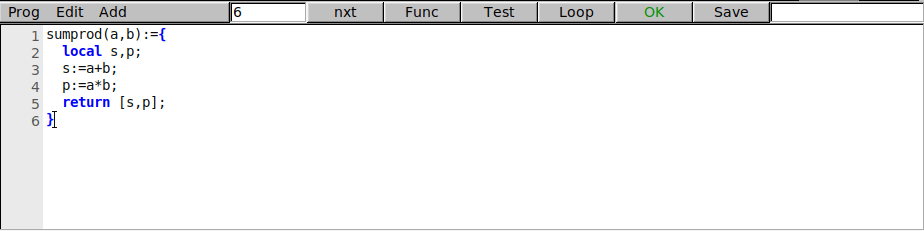
\includegraphics[width=\linewidth]{xcas-editor.png}
  \caption{\label{fig:editor}Programming editor in \xcas{}}
\end{figure}

\subsection{Functions%: \xcaskey{function} \xcaskey{endfunction} \texttt{\{} \texttt{\}} \xcaskey{local} \xcaskey{return}
  \label{ssec:funcs}}

You have already seen functions defined with \texttt{:=}.  For
example, to define a function \texttt{sumprod} which takes two inputs
and returns a list with the sum and the product of the inputs, you can
enter:
\begin{xcasinput}
sumprod(a,b):=[a+b,a*b]
\end{xcasinput}
Afterwards, use this new function.
\begin{xcasinput}
sumprod(3,5)
\end{xcasinput}
\begin{xcasoutput}
  \left[8,15\right]
\end{xcasoutput}

You can define functions that are computed with a sequence of
instructions by putting the instructions between braces\index{\{\}@\texttt{\{\}}},
where each command ends with a semicolon.  To use local variables,
you can declare them with the \xcaskey{local}\index{local@\xcaskey{local}}
keyword, followed by the
variable names.  The value returned by the function will be indicated
with the \xcaskey{return}\index{return@\xcaskey{return}} keyword.
For example, the above function \texttt{sumprod} could also be defined by:
\begin{lstlisting}
sumprod(a,b):={
  local s,p;
  s:=a+b;
  p:=a*b;
  return [s,p];
}
\end{lstlisting}
To avoid using braces, the \xcaskey{proc}\index{proc@\xcaskey{proc}}
and \xcaskey{end}\index{end@\xcaskey{end}} keywords may be used like this:
\begin{lstlisting}
sumprod:=proc(a,b)
  local s,p;
  s:=a+b;
  p:=a*b;
  return [s,p];
end
\end{lstlisting}
Yet another way to define a function is by using the
\xcaskey{function}\index{function@\xcaskey{function}}\ldots
\xcaskey{endfunction}\index{endfunction@\xcaskey{endfunction}}
construction. With this approach, the function name and parameters follow the
\xcaskey{function} keyword.  This is otherwise like the previous
approach.  The \texttt{sumprod} function could be defined by:
\begin{lstlisting}
function sumprod(a,b)
  local s,p;
  s:=a+b;
  p:=a*b;
  return [s,p];
endfunction
\end{lstlisting}

\subsection{Local variables}

Local variables in a function definition can be given initial values
in the line they are declared in by putting  their initialization in
parentheses; for example,
\begin{lstlisting}
local a,b;
a:=1;
\end{lstlisting}
is the same as
\begin{lstlisting}
local (a:=1), b;
\end{lstlisting}

Local variables should be given values within the function definition.
If you want to use a local variable as a symbolic variable, then you
can indicate that with the \texttt{assume\index{assume@\texttt{assume}}} command
(see \secref{ssec:about}).  For
example, if you define a function \texttt{myroots} by
\begin{lstlisting}
myroots (a):={
  local x;
  return solve(x^2=a,x);
}
\end{lstlisting}
then calling
\begin{xcasinput}
myroots(4)
\end{xcasinput}
will simply return the empty list.  You could leave \texttt{x}
undeclared, but that would make \texttt{x} a global variable and could
interact with other functions in unexpected ways.  You can get the
behavior you probably expected by explicitly assuming \texttt{x} to be a
symbol\index{symbol@\texttt{symbol}};
\begin{lstlisting}
myroots(a):={
  local x;
  assume(x,symbol);
  return solve(x^2=a,x);
}
\end{lstlisting}
(Alternatively, you could use \texttt{purge(x)\index{purge@\texttt{purge}}} instead
of \texttt{assume(x,symbol)}.) Now if you enter
\begin{xcasinput}
myroots(4)
\end{xcasinput}
you will get
\begin{xcasoutput}
  [-2,2]
\end{xcasoutput}

\subsection{Default values of the parameters}

You can give the parameters of a function default values by putting
\textit{parameter}\texttt{=}\textit{value} in the parameter list of
the function.  For example, if you define a function:
\begin{lstlisting}
f(x,y=5,z):={
  return x*y*z;
}
\end{lstlisting}
then:
\begin{xcasinput}
f(1,2,3)
\end{xcasinput}
\begin{xcasoutput}
  6
\end{xcasoutput}
since the product $1\cdot 2\cdot 3=6$.  If you give \texttt{f} only two
values as input:
\begin{xcasinput}
f(3,4)
\end{xcasinput}
\begin{xcasoutput}
  60
\end{xcasoutput}
since the values 3 and 4 will be given to the parameters which do not
have default values; in this case, \texttt{y} will get its default value \texttt{5} while
\texttt{3} and \texttt{4} will be assigned to \texttt{x} and
\texttt{z}, respectively.  The result is $x y z=3\cdot 5\cdot 4=60$.

\subsection{Programs}

A program\index{program@\texttt{program}} is similar to a function, and is written like a
function without a return value.  Programs are used to display results
or to create drawings.  It is a good idea to turn a program into a
function by putting \texttt{return 0} at the end; this way you will
get a response of \texttt{0} when the program executes.

\subsection{Scripts}

A script is a file containing a sequence of instructions, each ending
with a semicolon.

\subsection{Code blocks
  \label{ssec:codeblocks}}

A code block, such as used in defining functions, is a sequence of
statements delimited by braces or by \texttt{begin}\index{begin@\xcaskey{begin}}
and \texttt{end\index{end@\xcaskey{end}}}.  Each statement must end with a semicolon.
If the block makes up a function, you can step through it one
statement at a time by using the debugger\index{debugger} (see
\secref{sec:debug}).

\section{Basic instructions}

\subsection{Comments%: \texttt{//}
}

The characters \texttt{//}\index{//@\texttt{//}} indicate that you
are writing a comment\index{comments};
any text between \texttt{//} and the end of the line will be ignored
by \xcas{}.

\subsection{Input%: \texttt{input} \texttt{Input} \texttt{InputStr} \texttt{textinput} \texttt{output} \texttt{Output}
}

\paragraph{Creating input windows.}
The \texttt{input}\index{input@\texttt{input}}
or \texttt{Input}\index{Input@\texttt{Input}}
command prompts the user for the value of a variable.
\begin{itemize}
\item \texttt{input} takes an arbitrary number of commands:

  \textit{vars}, a sequence of variable names, each one optionally
  preceded by a string.
\item \texttt{input(}\textit{vars}\texttt{)} brings up a box where
  the user can enter a value for each variable.

  If a variable is preceded with a string, then that string will be
  the prompt for the variable, otherwise the variable name will be the
  prompt.
\end{itemize}

\subsubsection*{Examples}
\begin{xcasinput}
input(a)
\end{xcasinput}
\begin{xcasimage}
  \includeimage{xcas-inputa.png}
\end{xcasimage}
\begin{xcasinput}
input("Set a to the value: ",a)
\end{xcasinput}
\begin{xcasimage}
  \includeimage{xcas-inputprompta.png}
\end{xcasimage}
\begin{xcasinput}
input(a,bee,c)
\end{xcasinput}
\begin{xcasimage}
  \includeimage{xcas-inputabc.png}
\end{xcasimage}
\begin{xcasinput}
input("Set a to the value: ",a,bee,"Set c to this value: ",c)
\end{xcasinput}
\begin{xcasimage}
  \includeimage{xcas-inputpromptabc.png}
\end{xcasimage}

If the value that you enter for \texttt{input} is a string, it should
be between quotes.  If you want the user to enter a string without
having to use the quotes, use the
\texttt{InputStr}\index{InputStr@\texttt{InputStr}} 
or \texttt{textinput}\index{textinput@\texttt{textinput}} command,
which is just like \texttt{input} except that it will assume any input
is a string and so the user won't need to use quotes.

\paragraph{Creating output windows.}
The \texttt{output}\index{output@\texttt{output}}
or texttt{Output}\index{Output@\texttt{Output}}
command creates message windows.
\begin{itemize}
\item \texttt{output} takes
  \texttt{strs}, a sequence of strings or variables which represent
  strings.
\item \texttt{output(}\textit{strs}\texttt{)} creates a message
  window displaying the concatentation of the strings.
\end{itemize}

\subsubsection*{Examples}
\begin{xcasinput}
s:="message"
output("This is a ",s)
\end{xcasinput}
\begin{xcasimage}
  \includeimage{xcas-output.png}
\end{xcasimage}
Use \texttt{output} to add
information to the input window:
\begin{xcasinput}
input(output("Calculate p(a)"),"polynomial",p,"value",a)
\end{xcasinput}
\begin{xcasimage}
  \includeimage{xcas-inputoutput.png}
\end{xcasimage}

\subsection{Reading a single keystroke%: \texttt{getKey}
}

The \texttt{getKey}\index{getKey@\texttt{getKey}}
command gets the next keystroke.
\begin{itemize}
\item \texttt{getKey} takes no arguments.
\item \texttt{getKey()} returns the \ASCII{} code of the next keystroke.
\end{itemize}

For example, if you enter
\begin{xcasinput}
asciicode:=getKey()
\end{xcasinput}
and hit the \texttt{A} key, then the variable \texttt{asciicode}
will have the value $65$, which is the \ASCII{} code of capital A.

\subsection{Checking conditions%: \texttt{assert}
}

The \texttt{assert}\index{assert@\texttt{assert}}
command breaks out of a function with an error.
\begin{itemize}
\item \texttt{assert} takes
  \textit{bool}, a boolean.
\item \texttt{assert(}\textit{bool}\texttt{)} does nothing if
  \textit{bool} is true, it returns from the function with an error if
  \textit{bool} is false.
\end{itemize}

\subsubsection*{Example}
Define the function:
\begin{xcasinput}
sqofpos(x):={ assert(x>0); return x^2; }
\end{xcasinput}
then:
\begin{xcasinput}
sqofpos(4)
\end{xcasinput}
\begin{xcasoutput}
  16
\end{xcasoutput}
\begin{xcasinput}
sqofpos(-4)
\end{xcasinput}
\begin{xcasoutput}
  \text{``assert failure: x>0 Error: Bad Argument Value''}
\end{xcasoutput}
since $-4>0$ is false.

\subsection{Checking the type of the argument%: \texttt{type} \texttt{subtype} \texttt{compare} \texttt{getType}
  \label{ssec:type}}
\index{type@\texttt{type}}
\index{subtype@\texttt{subtype}}
\index{compare@\texttt{compare}}
\index{getType@\texttt{getType}}
\index{real@\texttt{real}}
\index{double@\textit{double}}
\index{DOM\_FLOAT@\textit{DOM\_FLOAT}}
\index{integer@\textit{integer}}
\index{DOM\_INT@\textit{DOM\_INT}}
\index{complex@\textit{complex}}
\index{DOM\_COMPLEX@\textit{DOM\_COMPLEX}}
\index{identifier@\textit{identifier}}
\index{DOM\_IDENT@\textit{DOM\_IDENT}}
\index{vector@\textit{vector}}
\index{DOM\_LIST@\textit{DOM\_LIST}}
\index{func@\textit{func}}
\index{DOM\_FUNC@\textit{DOM\_FUNC}}
\index{expression@\textit{expression}}
\index{DOM\_SYMBOLIC@\textit{DOM\_SYMBOLIC}}
\index{symbol@\textit{symbol}}
\index{rational@\textit{rational}}
\index{DOM\_RAT@\textit{DOM\_RAT}}
\index{string@\texttt{string}}
\index{DOM\_STRING@\textit{DOM\_STRING}}
\index{NUM@\textit{NUM}}
\index{VAR@\textit{VAR}}
\index{STR@\textit{STR}}
\index{EXPR@\textit{EXPR}}
\index{NONE@\textit{NONE}}
\index{PIC@\textit{PIC}}
\index{MAT@\textit{MAT}}
\index{FUNC@\textit{FUNC}}
\index{LIST@\textit{LIST}}

The \texttt{type} command finds the type of its input.
\begin{itemize}
\item \texttt{type} takes one argument: 
  \textit{arg}, an object.
\item \texttt{type(}\textit{arg}\texttt{)} returns an integer
  indicating the type of \textit{arg}.

  The integer is given as a constant symbol which is equal to the integer.
  The possible values are: 
  \begin{itemize}
  \item \texttt{1}, equivalently
    \texttt{real}, \texttt{double} or \texttt{DOM\_FLOAT}.
  \item \texttt{2}, equivalently
    \texttt{integer} or \texttt{DOM\_INT}.
  \item \texttt{4}, equivalently
    \texttt{complex} or \texttt{DOM\_COMPLEX}.
  \item \texttt{6}, equivalently
    \texttt{identifier} or \texttt{DOM\_IDENT}.
  \item \texttt{7}, equivalently
    \texttt{vector} or \texttt{DOM\_LIST}.
  \item \texttt{8}, equivalently
    \texttt{expression} or \texttt{DOM\_SYMBOLIC}.
  \item \texttt{10}, equivalently
    \texttt{rational} or \texttt{DOM\_RAT}.
  \item \texttt{12}, equivalently
    \texttt{string} or \texttt{DOM\_STRING}.
  \item \texttt{13}, equivalently
    \texttt{func} or \texttt{DOM\_FUNC}.
  \end{itemize}
\end{itemize}

The \texttt{getType} command is similar to \texttt{type} in that it
takes an object and returns the type, but it has different possible
return values.  It is included for compatibility reasons.
\begin{itemize}
\item \texttt{getType} takes
  \textit{obj}, an object.
\item \texttt{getType(}\textit{obj}\texttt{)} returns the type of
  \textit{obj}, which in this case means one of:
  \texttt{NUM}, \texttt{VAR}, \texttt{STR}, \texttt{EXPR},
  \texttt{NONE}, \texttt{PIC}, \texttt{MAT} or \texttt{FUNC}.
\end{itemize}

\subsubsection*{Examples}
\begin{xcasinput}
type(4)
\end{xcasinput}
\begin{xcasoutput}
  \text{integer}
\end{xcasoutput}
\begin{xcasinput}
type(3.1)==DOM_FLOAT
\end{xcasinput}
\begin{xcasoutput}
  \text{true}
\end{xcasoutput}
\begin{xcasinput}
getType(3.14)
\end{xcasinput}
\begin{xcasoutput}
  \text{NUM}
\end{xcasoutput}
\begin{xcasinput}
getType(x)
\end{xcasinput}
\begin{xcasoutput}
  \text{VAR}
\end{xcasoutput}

\subsubsection{Subtypes}
\xcas{} has various types of lists; the \texttt{subtype} command
can determine what kind of list it is.
\begin{itemize}
\item \texttt{subtype} takes
  $L$, a list (in \texttt{DOM\_LIST}).
\item \texttt{subtype($L$)} returns an integer indicating what type
  of list $L$ is.

  The possible values are:
  \begin{itemize}
  \item 1 is $L$ is a sequence.
  \item 2 if $L$ is a set.
  \item 10 if $L$ is a polynomial represented by a list (see
    \secref{sec:polynomials}).
  \item 0 if $L$ isn't one of the above types of list.
  \end{itemize}
\end{itemize}

\subsubsection*{Example}
\begin{xcasinput}
subtype(1,2,3)
\end{xcasinput}
\begin{xcasoutput}
  1
\end{xcasoutput}

\subsubsection{Object comparison}
The \texttt{compare} operator compares two objects taking their
type into account.
\begin{itemize}
\item \texttt{compare} takes two arguments:
  $a,b$, two objects.
\item \texttt{compare($a,b$)} returns
  \begin{itemize}
  \item  $1$ (\texttt{true}) if $\texttt{type}(a)<\texttt{type}(b)$ or if
    $\texttt{type}(a)=\texttt{type}(b)$ and $a$ is less than $b$ in the
    ordering of their type.
  \item $0$ (\texttt{false}) otherwise.
  \end{itemize}
\end{itemize}

\subsubsection*{Examples}
\begin{xcasinput}
compare("a","b")
\end{xcasinput}
\begin{xcasoutput}
  1
\end{xcasoutput}
since \texttt{"a"} and \texttt{"b"} have the same type
(\texttt{string}) and \texttt{"a"} is less than \texttt{"b"} in the
string ordering.

If \texttt{b} is a formal variable:
\begin{xcasinput}
compare("a",b)
\end{xcasinput}
\begin{xcasoutput}
  0
\end{xcasoutput}
since the type of \texttt{"a"} is \texttt{string} (the integer 12)
while the type of \texttt{b} is \texttt{identifier} (the integer 6)
and \texttt{12} is not less than \texttt{6}.

\subsection{Printing%: \texttt{print} \texttt{Disp} \texttt{ClrIO}
}

The \texttt{print}\index{print@\texttt{print}}
or \texttt{Disp}\index{Disp@\texttt{Disp}}
command prints in a special pane called message area, located
between input and output panes of a command line entry (the text
is shown in green).
\begin{itemize}
\item \texttt{print} takes
  \textit{seq}, a sequence of objects.
\item \texttt{print(}\textit{seq}\texttt{)} returns 1 and prints the
  \textit{seq} in a special pane just above the output line.
\end{itemize}

\subsubsection*{Examples}
\begin{xcasinput}
print("Hello")
\end{xcasinput}
\begin{xcasmsg}
  Hello
\end{xcasmsg}
\begin{xcasoutput}
  1
\end{xcasoutput}
\begin{xcasinput}
a:=12
print("a=",a)
\end{xcasinput}
\begin{xcasoutput}
  &\text{``a=,12''}\\
  &1
\end{xcasoutput}

The \texttt{ClrIO}\index{ClrIO@\texttt{ClrIO}}
command erases printing on the level it was typed.
\begin{itemize}
\item \texttt{ClrIO} takes no arguments and no parentheses.
\item \texttt{ClrIO} returns 1 and erases any printing on the
  special pane above the output line on the level it was typed.
\end{itemize}

\subsubsection*{Example}
\begin{xcasinput}
print("Hello"); ClrIO
\end{xcasinput}
\begin{xcasoutput}
  (1,1)
\end{xcasoutput}

\subsection{Displaying exponents%: \texttt{printpow}
}

The \texttt{printpow}\index{printpow@\texttt{printpow}}
command determines how the \texttt{print}
command will print exponents in the special pane above the output line.
\begin{itemize}
\item \texttt{printpow} takes
  $n$, which is either $-1$, $0$ or $1$ (by default 1).
\item \texttt{printpow($n$)} sets the style for printing exponents
  with the \texttt{print} command.
  \begin{itemize}
  \item If $n=-1$, \texttt{print($a$\^{}$b$)} will subsequently print
    \texttt{$a$**$b$)}.
  \item If $n=0$, \texttt{print($a$\^{}$b$)} will subsequently print
    \texttt{pow($a,b$)}.
  \item If $n=1$, \texttt{print($a$\^{}$b$)} will subsequently print
    $a$\texttt{\^{}}$b$.
  \end{itemize}
\end{itemize}

\subsubsection*{Examples}
\begin{xcasinput}
print(x^3):;
\end{xcasinput}
\begin{xcasmsg}
  x\verb|^|3
\end{xcasmsg}
\begin{xcasinput}
printpow(-1):; print(x^3):;
\end{xcasinput}
\begin{xcasmsg}
  x**3
\end{xcasmsg}
\begin{xcasinput}
printpow(0):; print(x^3):;
\end{xcasinput}
\begin{xcasmsg}
  pow(x,3)
\end{xcasmsg}
\begin{xcasinput}
printpow(1):; print(x^3):;
\end{xcasinput}
\begin{xcasmsg}
  x\verb|^|3
\end{xcasmsg}

\subsection{Infixed assignments%: \texttt{=>} \texttt{:=} \texttt{=<}
}

The infixed operators \texttt{=>}\index{=>@\texttt{=>}},
\texttt{:=}\index{:=@\texttt{:=}}, and
\texttt{=<}\index{=<@\texttt{=<}} can
all store a value in a variable, but their arguments are in different
order.  (See \secref{ssec:assign} and \secref{ssec:refassign}.)
Also, \texttt{:=} and \texttt{=<} have different effects when
the first argument is an element of a list stored in a variable, since
\texttt{=<} modifies list elements by reference (see section
\ref{ssec:assignmentdiffs}).

\texttt{=>} is the infixed version of \texttt{sto}, it stores
the value in the first argument in the variable in the second
argument.  Both
\begin{xcasinput}
4=>a
\end{xcasinput}
and
\begin{xcasinput}
sto(4,a)
\end{xcasinput}
store the value 4 in the variable \texttt{a}.

\texttt{:=} and \texttt{=<} both have a variable as the first
argument and the value to store in the variable as the second
argument. Both
\begin{xcasinput}
a:=4
\end{xcasinput}
and
\begin{xcasinput}
a=<4
\end{xcasinput}
store the value 4 in the variable \texttt{a}.

However, suppose you have entered:
\begin{xcasinput}
A:=[0,1,2,3,4]:; B:=A
\end{xcasinput}
  and you want to change \texttt{A[3]}, then the commandline
\begin{xcasinput}
A[3]=<33
\end{xcasinput}
  will change both \texttt{A} and \texttt{B}:
\begin{xcasinput}
A,B
\end{xcasinput}
\begin{xcasoutput}
  \left[0,1,2,33,4\right],\left[0,1,2,33,4\right]
\end{xcasoutput}
Here, \texttt{A} pointed to the list \texttt{[0,1,2,3,4]} and
after setting \texttt{B} to \texttt{A}, \texttt{B} also pointed to
\texttt{[0,1,2,3,4]}.  Changing an element of \texttt{A} by
reference changes the list that \texttt{A} points to, which
\texttt{B} also points to.

Note that multiple assigments can be made using sequences or lists.
Both
\begin{xcasinput}
[a,b,c]:=[1,2,3]
\end{xcasinput}
and
\begin{xcasinput}
(a,b,c):=(1,2,3)
\end{xcasinput}
assign \texttt{a} the value 1, \texttt{b} the value 2, and \texttt{c}
the value 3.  If multiple assignments are made this way and variables
are on the right hand side, they will be replaced by their values
before the assignment.  If \texttt{a} contains 5 and you enter:
\begin{xcasinput}
(a,b):=(2,a)
\end{xcasinput}
then \texttt{b} will get the previous value of \texttt{a}, 5, and not
the new value of \texttt{a}, 2.

\subsection{Assignment by copying%: \texttt{copy}
}

The \texttt{copy}\index{copy@\texttt{copy}}
command creates a copy of its argument, which is
typically a list of some type.  If \texttt{B} is a list and \texttt{A:=B},
then \texttt{A} and \texttt{B} point to the same list, and so
changing one will change the other.  But if \texttt{A:=copy(B)}, then
\texttt{A} and \texttt{B} will point to different lists with the same
values, and so can be changed individually.

\subsubsection*{Example}
\begin{xcasinput}
B:=[[4,5],[2,6]]:;
A:=B:;
C:=copy(B):;
A,B,C
\end{xcasinput}
\begin{xcasoutput}
  \begin{bmatrix}4&5\\2&6\end{bmatrix},\begin{bmatrix}4&5\\2&6\end{bmatrix},\begin{bmatrix}4&5\\2&6\end{bmatrix}
\end{xcasoutput}
\begin{xcasinput}
B[1]=<[0,0]:;
A,B,C
\end{xcasinput}
\begin{xcasoutput}
  \begin{bmatrix}4&5\\0&0\end{bmatrix},\begin{bmatrix}4&5\\0&0\end{bmatrix},\begin{bmatrix}4&5\\2&6\end{bmatrix}
\end{xcasoutput}

\subsection{Difference between operators \texttt{:=} and \texttt{=<}\label{ssec:assignmentdiffs}}

The \texttt{:=} and \texttt{=<} assignment operators have different
effects when they are used to modify an element of a list contained in
a variable, since \texttt{=<} modifies the element by reference.
Otherwise, they will have the same effect.

\subsubsection*{Example}
\begin{xcasinput}
A:=[1,2,3]
\end{xcasinput}
Now
\begin{xcasinput}
A[1]:=5
\end{xcasinput}
and
\begin{xcasinput}
A[1]=<5
\end{xcasinput}
both change \texttt{A[1]} to 5:
\begin{xcasinput}
A
\end{xcasinput}
\begin{xcasoutput}
  \left[1,5,3\right]
\end{xcasoutput}
but they do it in different ways.  The command
\texttt{A[1]=<5} changes the middle value in the list that
\texttt{A} originally pointed to, and so any other variable pointing
to the list will be changed, but \texttt{A[1]:=5} will create a
duplicate list with the middle element of 5, and so any other variable
pointing to the original list won't be affected.

\subsubsection*{Examples}
\begin{xcasinput}
A:=[0,1,2,3,4]:;
B:=A:;
B[3]=<33:;
A,B
\end{xcasinput}
\begin{xcasoutput}
  \left[0,1,2,33,4\right],\left[0,1,2,33,4\right]
\end{xcasoutput}
\begin{xcasinput}
A:=[0,1,2,3,4]:;
B:=A:;
B[3]:=33:;
A,B
\end{xcasinput}
\begin{xcasoutput}
  \left[0,1,2,3,4\right],\left[0,1,2,33,4\right]
\end{xcasoutput}
If \texttt{B} is set equal to a copy of \texttt{A} instead of
\texttt{A}, then changing \texttt{B} won't affect \texttt{A}.
\begin{xcasinput}
A:=[0,1,2,3,4];
B:=copy(A);
B[3]=<33;
A,B
\end{xcasinput}
\begin{xcasoutput}
  \left[0,1,2,3,4\right],\left[0,1,2,33,4\right]
\end{xcasoutput}

\section{Control structures}

\subsection{Conditional statements%: \xcaskey{if} \xcaskey{then} \xcaskey{else} \xcaskey{end} \xcaskey{elif}
}

The \xcas{} language has different ways of writing
``if\ldots then'' statements (see \secref{ssec:piecewise}).
The standard version of such a statement consists of
the \xcaskey{if}\index{if@\xcaskey{if}} keyword, followed by a boolean expression (see
\secref{sec:boolean}) in parentheses, followed by a statement block
(see \secref{ssec:codeblocks}) which will be executed if the boolean
is true.  You can optionally add an \xcaskey{else}\index{else@\xcaskey{else}}
keyword followed by a statement block which will be executed if the boolean is false.
\begin{center}
  \xcaskey{if} \texttt{(}\textit{boolean}\texttt{)} \textit{true-block} $\langle$\xcaskey{else} \textit{false-block}$\rangle$
\end{center}
Recall that the blocks need to be delimited by braces or by
\xcaskey{begin} and \xcaskey{end}.

\subsubsection*{Examples}
\begin{xcasinput}
a:=3:; b:=2:;
if (a>b) { a:=a+5; b:=a-b; }:;
a,b
\end{xcasinput}
\begin{xcasoutput}
  8,6
\end{xcasoutput}
since \texttt{a>b} evaluates to true, and so the variable
\texttt{a} resets to \texttt{8} and \texttt{b} resets
to the value \texttt{6}.
\begin{xcasinput}
a:=3:; b:=2:;
if (a<b) { a:=a+5; b:=a-b; } else { a:=a-5; b:=a+b; }:;
a,b
\end{xcasinput}
\begin{xcasoutput}
  -2,0
\end{xcasoutput}
since \texttt{a>b} evaluates to false, and so the variable
\texttt{a} resets to \texttt{-2} and \texttt{b} resets
to the value \texttt{0}.

\paragraph{The ``if\ldots then\ldots else\ldots end'' structure.}
An alternate way to write an \xcaskey{if} statement is to enclose the
code block in \xcaskey{then}\index{then@\xcaskey{then}} and
\xcaskey{end}\index{end@\xcaskey{end}} instead of braces:
\begin{center}
  \xcaskey{if} \texttt{(}\textit{boolean}\texttt{)} \xcaskey{then} \textit{true-block} $\langle$\xcaskey{else} \textit{false-block}$\rangle$ \xcaskey{end}
\end{center}
\begin{itemize}
\item In this case, it is usually not necessary to enclose the boolean in parentheses.
\item Instead of the keyword \xcaskey{end}, you can also use \xcaskey{fi}\index{fi@\xcaskey{fi}}.
\end{itemize}

\subsubsection*{Examples}
\begin{xcasinput}
a:=3:;
if a>1 then a:=a+5; end
\end{xcasinput}
\begin{xcasoutput}
  8
\end{xcasoutput}
\begin{xcasinput}
a:=8:;
if a>10 then a:=a+10; else a:=a-5; end
\end{xcasinput}
\begin{xcasoutput}
  3
\end{xcasoutput}
This input can also be written as:
\begin{xcasinput}
si a>10 alors a:=a+10; sinon a:=a-5; fsi
\end{xcasinput}

\paragraph{Nesting conditional statements.}
Several \xcaskey{if} statements can be nested. For example:
\begin{lstlisting}
if a>1 then a:=1; else if a<0 then a:=0; else a:=0.5; end; end
\end{lstlisting}
A simpler way is to replace the \xcaskey{else}~\xcaskey{if} by
\xcaskey{elif}\index{elif@\xcaskey{elif}} and
combine the \xcaskey{end}s:
\begin{lstlisting}
if a>1 then a:=1; elif a<0 then a:=0; else a:=0.5; end
\end{lstlisting}
In general, such a combination can be written
\begin{center}
  \begin{tabular}{l} 
    \xcaskey{if} \texttt{(}\textit{boolean1}\texttt{)} \xcaskey{then}\\
    \textit{~~block1;}\\
    \xcaskey{elif} \texttt{(}\textit{boolean2}\texttt{)} \xcaskey{then}\\
    \textit{~~block2;}\\
    \ldots\\
    \xcaskey{elif} \texttt{(}\textit{booleanN}\texttt{)} \xcaskey{then}\\
    \textit{~~blockN;}\\
    \xcaskey{else}\\
    \textit{~~last block;}\\
    \xcaskey{end}
  \end{tabular}
\end{center}
where the last \xcaskey{else} is optional.
For example, to define a function $f$ by
\[
  f(x)=
  \begin{cases}
    8 & \text{if } x > 8\\
    4 & \text{if } 4 < x \le 8\\
    2 & \text{if } 2 < x \le 4\\
    1 & \text{if } 0 < x \le 2\\
    0 & \text{if } x \le 0
  \end{cases}
\]
you may enter:
\begin{lstlisting}
f(x):={
  if (x>8) then
  return 8;
  elif (x>4) then
  return 4;
  elif (x>2) then
  return 2;
  elif (x>0) then
  return 1;
  else
  return 0;
  fi;
}
\end{lstlisting}

\subsection{Switch statement%: \xcaskey{switch} \xcaskey{case} \xcaskey{default}
}

The \xcaskey{switch}\index{switch@\xcaskey{switch}}
statement can be used when you want the value of a
block to depend on an integer.  It takes one argument, an expression
which evaluates to an integer.  It should be followed by a sequence of
\xcaskey{case}\index{case@\xcaskey{case}} statements, which takes
the form \xcaskey{case} followed
by an integer and then a colon, which is followed by a code block to
be executed if the expression equals the integer.  At the end is an
optional \xcaskey{default}\index{default@\xcaskey{default}}
statement, which is followed by a code block to be executed if the
expression does not equal any of the given integers.
\begin{center}
  \begin{tabular}{l}
    \xcaskey{switch}\texttt{($n$) \{}\\
    \texttt{~~}\xcaskey{case} $n_1$: \textit{block $n_1$}\\
    \texttt{~~}\xcaskey{case} $n_2$: \textit{block $n_2$}\\
    ~~~\ldots\\
    \texttt{~~}\xcaskey{case} $n_k$: \textit{block $n_k$}\\
    \texttt{~~}\xcaskey{default}: \textit{default\_block}
  \end{tabular}
\end{center}
Recall that the blocks need to be delimited by braces or by
\xcaskey{begin} and \xcaskey{end}.

\subsubsection*{Example}
As an example of a program which performs an operation on the first
two variables depending on the third, you could enter (see
\secref{ssec:proged}):
\begin{lstlisting}
oper(a,b,c):={
  switch (c) {
    case 1:  { a:=a+b; break; }
    case 2:  { a:=a-b; break; }
    case 3:  { a:=a*b; break; }
    default: { a:=a^b; }
  }
  return a;
}
\end{lstlisting}
Then:
\begin{xcasinput}
oper(2,3,1)
\end{xcasinput}
\begin{xcasoutput}
  5
\end{xcasoutput}
since the third argument is \texttt{1}, and so \texttt{oper(a,b,c)}
will return $a+b$, and:
\begin{xcasinput}
oper(2,3,2)
\end{xcasinput}
\begin{xcasoutput}
  -1
\end{xcasoutput}
since the third argument is \texttt{2} and so \texttt{oper(a,b,c)}
will return $a-b$.


\subsection{For loop%: \xcaskey{for} \xcaskey{from} \xcaskey{to} \xcaskey{step} \xcaskey{do} \xcaskey{end\_for}
  \label{ssec:for}}

The for-loop has three different forms, each of which uses an
index variable.  If the for-loop is used in a program, the
index variable should be declared as a local variable.  (Recall that
\texttt{i} represents the imaginary unit, and so cannot be used as the
index.)

\paragraph{The first form.}
For the first form, the \xcaskey{for}\index{for@\xcaskey{for}} keyword is
followed by the starting value for the index, the end condition, and
the increment step, separated by semicolons and in parentheses.
Afterwards is a block of code to be executed for each iteration,
where $j$ is the index and $j_0$ is the starting value of $j$:
\begin{center}
  \xcaskey{for} \texttt{($j$:=$j_0$;~}\textit{end\_cond}\texttt{;~}\textit{increment\_step}\texttt{)} \textit{block}
\end{center}

\subsubsection*{Example}
To add the even numbers less than 100, you can start by setting the
running total to 0:
\begin{xcasinput}
S:=0
\end{xcasinput}
Then use a \xcaskey{for} loop to do the summation:
\begin{xcasinput}
for (j:=0;j<100;j:=j+2) { S:=S+j }
\end{xcasinput}
\begin{xcasoutput}
  2450
\end{xcasoutput}


\paragraph{The second form.}
The second form of a for-loop has a fixed increment for the index.
It is written out with the \xcaskey{for}\index{for@\xcaskey{for}} keyword
followed by the index, then \xcaskey{from}\index{from@\xcaskey{from}},
the initial value,
\xcaskey{to}\index{to@\xcaskey{to}}, the ending value,
\xcaskey{step}\index{step@\xcaskey{step}}, the size of the
increment, and finally the statements to be executed between
\xcaskey{do} and \xcaskey{end\_for}:
\begin{center}
  \xcaskey{for} $j$ \xcaskey{from} $j_0$ \xcaskey{to} $j_{max}$ \xcaskey{step} $k$ \xcaskey{do} \textit{statements} \xcaskey{end\_for}
\end{center}
where $j$ is the index, $j_0$ is the initial value of $j$, $j_{max}$
is the ending value of $j$, $k$ is the step size of $j$, and
\textit{statements} are executed for each value of $j$.

\subsubsection*{Example}
Again, to add the even numbers less than 100, you can start by setting the
running total to 0:
\begin{xcasinput}
S:=0
\end{xcasinput}
then use the second form of the \xcaskey{for} loop to do the summation:
\begin{xcasinput}
for j from 2 to 98 step 2 do S:=S+j; end_for
\end{xcasinput}
or (a French version of this syntax):
\begin{xcasinput}
pour j de 2 jusque 98 pas 2 faire S:=S+j; fpour
\end{xcasinput}
\begin{xcasoutput}
  2450
\end{xcasoutput}

\paragraph{The third form.}
The third form of a for-loop lets you iterate over the values in a
list (or a set or a range).  In this form, the
\xcaskey{for}\index{for@\xcaskey{for}} keyword is followed by the index, then
\xcaskey{in}\index{in@\xcaskey{in}}, the list, and then the instructions between
\xcaskey{do}\index{do@\xcaskey{do}}
and \xcaskey{end\_for}\index{end\_for@\xcaskey{end\_for}} or
\xcaskey{od}\index{od@\xcaskey{od}}:
\begin{center}
  \xcaskey{for} $j$ \xcaskey{in} $L$ \xcaskey{do} \textit{statements} \xcaskey{end\_for}
\end{center}
where $j$ is the index and $L$ is the list to iterate over.

\subsubsection*{Example}
To add all integers from 1 to 100, you can again set the running total
\texttt{S} to 0:
\begin{xcasinput}
S:=0
\end{xcasinput}
then use the third form of the \xcaskey{for} loop to add the integers:
\begin{xcasinput}
for j in 1..100 do S:=S+j; end_for
\end{xcasinput}
or:
\begin{xcasinput}
pour j in 1..100 faire S:=S+j; fpour
\end{xcasinput}
\begin{xcasoutput}
  5050
\end{xcasoutput}

\subsection{Repeat loop%: \xcaskey{repeat} \xcaskey{until}
}

The repeat-loop allows you to repeat statements until a given
condition is met.  To use it, enter \xcaskey{repeat}\index{repeat@\xcaskey{repeat}},
the statements, the keyword \xcaskey{until}\index{until@\xcaskey{until}}
followed by the condition, a boolean:
\begin{center}
  \xcaskey{repeat} \textit{statements} \xcaskey{until} \textit{bool}
\end{center}

\subsubsection*{Example}
If you want the user to enter a value for a variable
\texttt{x} which is greater than 4, you could use:
\begin{lstlisting}
repeat
  input("Enter a value for x (greater than 4)",x);
until (x>4);
\end{lstlisting}
which could also be written as
\index{repeter@\xcaskey{repeter}}\index{jusqua@\xcaskey{jusqua}}
\begin{lstlisting}
repeter
  input("Enter a value for x (greater than 4)",x);
jusqua (x>4);
\end{lstlisting}

\subsection{While loop%: \xcaskey{while}
}

The while-loop is used to repeat a code block as long as a
given condition holds.  To use it, enter
\xcaskey{while}\index{while@\xcaskey{while}}, the
condition in parentheses, and then a code block.
\begin{center}
  \xcaskey{while} \texttt{(}\textit{boolean}\texttt{)} \textit{block}
\end{center}

\subsubsection*{Example}
Add the terms of
the harmonic series $1+\frac12+\frac13+\frac14+\cdots$ until a term is less
than 0.05.

You can initialize the sum \texttt{S} to 0 and let
\texttt{j} be the first term 1. Input:
\begin{xcasinput}
S:=0; j:=1
\end{xcasinput}
Then use a while loop.
\begin{xcasinput}
while (1/j>=0.05) { S:=S+1/j; j:=j+1; }
\end{xcasinput}
or:
\begin{xcasinput}
tantque (1/j>=0.05) faire S:=S+1/j; j:=j+1; ftantque
\end{xcasinput}
then:
\begin{xcasinput}
S
\end{xcasinput}
\begin{xcasoutput}
  \frac{55835135}{15519504}
\end{xcasoutput}
Note that a \xcaskey{while} loop can also be written as a \xcaskey{for}
loop.  For example, as long as \texttt{S} is set to 0 and \texttt{j}
is set to 1, the above loop can be written as
\begin{xcasinput}
for (;1/j>=0.05;) { S:=S+1/j; j:=j+1; }
\end{xcasinput}
or, with only \texttt{S} set to 0,
\begin{xcasinput}
for (j:=1; 1/j>=0.05; j++) { S:=S+1/j; }
\end{xcasinput}
which, of course, yields the same result.

\subsection{Breaking out of loop%: \xcaskey{break}
}

The \xcaskey{break}\index{break@\xcaskey{break}}
command exits a loop without finishing it.
\begin{itemize}
\item \xcaskey{break} takes no arguments or parentheses.
\item \xcaskey{break} exits the current loop.
\end{itemize}

\subsubsection*{Example}
Define a program:
\begin{lstlisting}
testbreak(a,b):={
  local r;
  while (true) {
    if (b==0) { break; }
    r:=irem(a,b);
    a:=b;
    b:=r;
  }
  return a;
}
\end{lstlisting}
Then:
\begin{xcasinput}
testbreak(4,0)
\end{xcasinput}
\begin{xcasoutput}
  4
\end{xcasoutput}
since the \xcaskey{while} loop is interrupted when \texttt{b} is 0 and
\texttt{a} is 4.

\subsection{Skipping to the next iteration of a loop%: \xcaskey{continue}
}

The \xcaskey{continue}\index{continue@\xcaskey{continue}}
command will skip the rest of the current
iteration of a loop and go to the next iteration.
\begin{itemize}
\item \xcaskey{continue} takes no arguments or parentheses.
\item \xcaskey{continue} goes to the next iteration of the current
  loop without finishing the current iteration.
\end{itemize}

\subsubsection*{Example}
If you enter:
\begin{lstlisting}
S:=0;
for (j:=1,j<=10;j++) {
  if (j==5) { continue; }
  S:=S+j;
}
\end{lstlisting}
then \texttt{S} will be 50, which is the sum of the integers from 1 to
10 except for 5, since the loop never gets to \texttt{S:=S+j} when
\texttt{j} is equal to 5.

\subsection{Changing the order of execution%: \xcaskey{goto} \xcaskey{label}
}

The \xcaskey{goto}\index{goto@\xcaskey{goto}}
command will tell a program to jump to a different
spot in a program, where the spot needs to have been marked with
\xcaskey{label}\index{label@\xcaskey{label}}.
They both must have the same argument, which is
simply a sequence of characters.
\begin{itemize}
\item \xcaskey{label} takes
  \textit{mark}, a sequence of characters.
\item \texttt{label(}\textit{mark}\texttt{)} labels the position in
  the program with \textit{mark}.
\end{itemize}
\begin{itemize}
\item \xcaskey{goto} takes
  \textit{mark}, a sequence of characters.
\item \texttt{goto(}\texttt{mark}\texttt{)} goes to the part of the
  program labeled with \textit{mark}.
\end{itemize}

\subsubsection*{Example}
The following program
will add the terms of the harmonic series until the term is less than
some specified value \texttt{eps} and print the result.
\begin{lstlisting}
harmsum(eps):={
  local S,j;
  S:=0;
  j:=0;
  label(spot);
  j:=j+1;
  S:=S+1/j;
  if (1/j>=eps) goto (spot);
  print(S);
  return 0;
}
\end{lstlisting}

\section{Errors}

\subsection{Handling errors%: \xcaskey{try} \xcaskey{catch} \xcaskey{throw} \texttt{error} \texttt{ERROR}
}

Some commands produce errors, and if your program tries to run such a
command it will halt with an error. 
The \xcaskey{try}\index{try@\xcaskey{try}} and
\xcaskey{catch}\index{catch@\xcaskey{catch}}
commands can help you to avoid halting the program;
put potentially problematic statements in a block
following \xcaskey{try}, and immediately after the block put
\xcaskey{catch} with an argument of an unused symbol, and follow that
with a block of statements that can handle the error.
\begin{center}
  \xcaskey{try} \textit{tryblock} \xcaskey{catch} (\textit{symbol}) \textit{catchblock}
\end{center}
If \textit{tryblock} does not produce an error,
then the code
\begin{center}
  \xcaskey{catch} (\textit{symbol}) \textit{catchblock}
\end{center}
is not reached. Otherwise,
if \textit{tryblock} does produce an error, then a
string describing the error is assigned to \textit{symbol},
and \textit{catchblock} is evaluated.

\subsubsection*{Examples}
The command below produces an error:
\begin{xcasinput}
[[1,1]]*[[2,2]]
\end{xcasinput}
\begin{xcasoutput}
  \text{Error: Invalid dimension}
\end{xcasoutput}
However, the following command does not produce an error:
\begin{xcasinput}
try { [[1,1]]*[[2,2]] } catch (err) { print("The error is --- "+err) }
\end{xcasinput}
\begin{xcasmsg}
The error is ---  Error: Invalid dimension
\end{xcasmsg}
\begin{xcasoutput}
  1
\end{xcasoutput}

With the following program:
\begin{lstlisting}
test(x):={
  local y,str,err;
  try {
    y:=[[1,1]]*x;
    str:="This produced a product.";
  } catch (err) {
    y:=x;
    str:="This produced an error "+err+" The input is returned.";
  }
  print(str);
  return y;
}
\end{lstlisting}
input:
\begin{xcasinput}
test([[2],[2]])
\end{xcasinput}
\begin{xcasoutput}
  &\text{``This produced a product.''}\\
  &\left[4\right]
\end{xcasoutput}
with the text in the pane above the output line.
\begin{xcasinput}
test([[2,2]])
\end{xcasinput}
\begin{xcasoutput}
  &\text{``This produced an error  Error:~Invalid dimension The input is returned.''}\\
  &\left[\left[2,2\right]\right]
\end{xcasoutput}
with the text in the pane above the output line.

You can catch this error in other programs.  Consider the program:
\begin{lstlisting}
g(x):={
  try {
    return f(x);
  } catch (err) {
    x:=0;
  }
  return x;
}
\end{lstlisting}
then:
\begin{xcasinput}
g(12)
\end{xcasinput}
\begin{xcasoutput}
  12
\end{xcasoutput}
since 12 is an integer. With a non-integer input, \texttt{f(x)} gives an error and so
\texttt{g(x)} returns 0:
\begin{xcasinput}
g(1.2)
\end{xcasinput}
\begin{xcasoutput}
  0
\end{xcasoutput}

\subsection{Throwing exceptions}

You can produce your own string to describe an error message with the
\xcaskey{throw}\index{throw@\xcaskey{throw}} or
\texttt{error}\index{error@\texttt{error}} or
\texttt{ERROR}\index{ERROR@\texttt{ERROR}} command.
\begin{itemize}
\item \xcaskey{throw} takes
  \textit{str}, a string describing an error.
\item \texttt{throw(}\textit{str}\texttt{)} generates an error with
  error string \textit{str}, possibly to be caught by \xcaskey{catch}.
\end{itemize}

\subsubsection*{Example}
With the following program:
\begin{lstlisting}
f(x):={
  if (type(x)!=DOM\_INT)
    throw("Not an integer");
  else
    return x;
}
\end{lstlisting}
input:
\begin{xcasinput}
f(12)
\end{xcasinput}
\begin{xcasoutput}
  12
\end{xcasoutput}
since 12 is an integer.
\begin{xcasinput}
f(1.2)
\end{xcasinput}
will signal an error
\begin{xcasoutput}
  \texttt{Not an integer Error:~Bad Argument Value}
\end{xcasoutput}
since 1.2 in not an integer.


\section{Other useful instructions}

\subsection{Defining a function with a variable number of arguments%: \texttt{args}
}

The \texttt{args}\index{args@\texttt{args}}
command returns the list of arguments of a function.
\begin{itemize}
\item \texttt{args} takes no arguments.
\item \texttt{args} (or \texttt{args(NULL)}) returns a list of the
  arguments of the current function, starting with the name of the
  function at index 0.
\end{itemize}
Note that \texttt{args()} will not work, the command must be called as
\texttt{args} or \texttt{args(NULL)}.  You can also use
\texttt{(args)[0]} to get the name of the function and
\texttt{(args)[1]} to get the first argument, etc., but the
parentheses about \texttt{args} is mandatory.

\subsubsection*{Examples}
\begin{xcasinput}
testargs():={ local y; y:=args; return y[1]; }:;
testargs(12,5)
\end{xcasinput}
\begin{xcasoutput}
  12
\end{xcasoutput}

As an another example, enter the function:
\begin{lstlisting}
total():={
  local s,a;
  a:=args;
  s:=0;
  for (k:=1;k<size(a);k++) {
    s:=s+a[k];
  }
  return s;
}
\end{lstlisting}
then:
\begin{xcasinput}
total(1,2,3,4)
\end{xcasinput}
\begin{xcasoutput}
  10
\end{xcasoutput}

\subsection{Assignments in a program}

Recall that the \texttt{=<} operator will change the value of a single
entry in a list or matrix by reference (see \secref{ssec:refassign}).
This make it efficient when changing many values, one at a time, in a
list, as might be done by a program.

You must be careful when doing this, since your intent might be
changed when a program is compiled.  For example, if a program contains
\begin{lstlisting}
local a;
a:=[0,1,2,3,4];
...
a[3]=<33;
\end{lstlisting}
then in the compiled program, \texttt{a:=[0,1,2,3,4]} will be
replaced by \texttt{a:=[0,1,2,33,4]}.  To avoid this, you can assign
a copy of the list to \texttt{a}; you could write:
\begin{lstlisting}
local a;
a:=copy([0,1,2,3,4]);
...
a[3]=<33;
\end{lstlisting}
Alternately, you could use a command which recreates a list every time
the program is run, such as \texttt{makelist\index{makelist@\texttt{makelist}}} or
\texttt{\$}, instead of copying a list;  \texttt{a:=makelist(n,n,0,4)} or
\texttt{a:=[n\$(n=0..4)]} can also be used in
place of \texttt{a:=[0,1,2,3,4]}.

\subsection{Writing variable values to a file%: \texttt{write}
  \label{ssec:write}}

The \texttt{write}\index{write@\texttt{write}}
command saves variable values to a file, to be read later.
\begin{itemize}
\item \texttt{write} takes two arguments:
  \begin{itemize}
  \item \textit{filename}, a string.
  \item \textit{vars}, a sequence of variables.
  \end{itemize}
\item \texttt{write(}$\textit{filename},\textit{vars}$\texttt{)}
  writes the variables in \textit{vars} assigned to their values in a
  file named \textit{filename}.
\end{itemize}

\subsubsection*{Example}
\begin{xcasinput}
a:=3.14
b:=7
write("foo",a,b)
\end{xcasinput}
creates a file named ``foo'' containing:
\begin{lstlisting}
a:=(3.14);
b:=7;
\end{lstlisting}
If you wanted to store the first million digits of $\pi$ to a file,
you could set it equal to a variable and store it in a file:
\begin{xcasinput}
pidec:=evalf(pi,10^6):;
write("pi1million",pidec)
\end{xcasinput}

The file is written so that it can be loaded with the \texttt{read}
command (\secref{ssec:read}), which simply takes a file name as a
string.  This allows you to  restore the values of variables saved
this way, for example in a different session or if you have purged the
variables.

\subsubsection*{Example}
If, in a different session, you want to use the
values of \texttt{a} and \texttt{b} above, enter:
\begin{xcasinput}
read("foo")
\end{xcasinput}
This will reassign the values \texttt{3.14} and \texttt{7} to
\texttt{a} and \texttt{b}.  Be careful, this will silently overwrite
any values that \texttt{a} and \texttt{b} might have had.

\subsection{Writing output to a file%: \texttt{fopen} \texttt{fclose} \texttt{fprint}
}

\xcas{} has a basic file I/O support in form of three commands:
\texttt{fopen}, \texttt{fprint} and \texttt{fclose}. Note that
reading from files is not supported.

The \texttt{fopen}\index{fopen@\texttt{fopen}}
command creates and opens a file to write into.
\begin{itemize}
\item \texttt{fopen} takes
  \textit{filename}, a string.
\item \texttt{fopen(}\textit{filename}\texttt{)} creates a file
  named \textit{filename} (and erases it if it already exists).
\end{itemize}
To use this, you need to associate it with a variable
\textit{var}\texttt{:=fopen(}\textit{filename}\texttt{)}
which use to refer to the file when printing to it.

The \texttt{fprint}\index{fprint@\texttt{fprint}}
command writes to a file.
\begin{itemize}
\item \texttt{fprint} takes two mandatory arguments and one optional
  argument:
  \begin{itemize}
  \item \textit{var}, a variable name associated with a file through
    \texttt{fopen}.
  \item Optionally,
    \texttt{Unquoted}\index{Unquoted@\textit{Unquoted}}, the symbol.
  \item \textit{info}, a list of what you want to write to the file.
  \end{itemize}
\item \texttt{fprint(}$\textit{var}\,\langle,\texttt{Unquote}\,\rangle,\textit{info}$\texttt{)} writes
  \textit{info} into the file given by \textit{var}. 
  By default, strings in \textit{info} are written with their
  quotation marks, with the option \texttt{Unquoted}, \texttt{fprint}
  will print them with the quotation marks.
\end{itemize}

The \texttt{fclose}\index{fclose@\texttt{fclose}}
command closes a previously opened file.
\begin{itemize}
\item \texttt{fclose} takes
  \textit{var}, a variable assigned to a file with \texttt{fopen}.
\item \texttt{fclose(}\textit{var}\texttt{)} closes the file given
  by \textit{var} to further writing.
\end{itemize}

\subsubsection*{Example}
To write contents to a file, you first need to open the file and
associate it with a variable.
\begin{xcasinput}
f:=fopen("bar")
\end{xcasinput}
This creates a file named ``bar'' (and so erase it if it already
exists).  To write to the file:
\begin{xcasinput}
x:=9:; fprint(f,"x+1 is ",x+1)
\end{xcasinput}
This puts
\begin{lstlisting}
"x+1 is "10
\end{lstlisting}
in the file.  Note that the quotation marks are not inserted if you use the
\texttt{Unquoted} argument:
\begin{xcasinput}
x:=9:; fprint(f,Unquoted,"x+1 is ",x+1)
\end{xcasinput}
This puts
\begin{lstlisting}
x+1 is 10
\end{lstlisting}
in the file.  Finally, after you have finished writing what you want
into the file, you close the file with the \texttt{fclose} command:
\begin{xcasinput}
fclose(f)
\end{xcasinput}
This returns \texttt{1} on success and \texttt{0} on failure.

\subsection{Converting strings to \giac{} expressions%: \texttt{expr}
}

\paragraph{Using strings as commands.}
The \texttt{expr}\index{expr@\texttt{expr}}
command lets you use a string as a command.
\begin{itemize}
\item \texttt{expr} takes
  \texttt{str}, a string which expresses a valid command.
\item \texttt{expr(}\textit{str}\texttt{)} converts \textit{str} to
  the command and evaluates it.
\end{itemize}

\subsubsection*{Examples}
\begin{xcasinput}
expr("c:=1"):;
c
\end{xcasinput}
\begin{xcasoutput}
  1
\end{xcasoutput}
\begin{xcasinput}
a:="ifactor(54)":;
expr(a)
\end{xcasinput}
\begin{xcasoutput}
  2\cdot 3^{3}
\end{xcasoutput}
which is the same thing as entering \texttt{ifactor(54)} directly.

\paragraph{Converting strings to numbers.}
You can also use \texttt{expr} to convert a string to a number. If a
string is simply a number enclosed by quotation marks, then
\texttt{expr} will return the number.

\subsubsection*{Examples}
% \begin{xcasinput}
% expr("123")
% \end{xcasinput}
% \begin{xcasoutput}
%   123
% \end{xcasoutput}
The following strings will be converted to the
appropriate number.

A string consisting of the digits 0-9 which does not start
with 0 will be converted to an integer:
\begin{xcasinput}
expr("2133")
\end{xcasinput}
\begin{xcasoutput}
  2133
\end{xcasoutput}
A string consisting of the digits 0-9 which contains a
single decimal point will be converted to a double:
\begin{xcasinput}
expr("123.4")
\end{xcasinput}
\begin{xcasoutput}
  123.4
\end{xcasoutput}
A string consisting of the digits 0-9 and a single decimal point,
followed by \texttt{e} and then more digits,
will be read as a floating point number:
\begin{xcasinput}
expr("1.23e4")
\end{xcasinput}
\begin{xcasoutput}
  12300.0
\end{xcasoutput}
A string consisting of the digits 0-7 which  starts
with 0 will be read as an integer base 8:
\begin{xcasinput}
expr("0176")
\end{xcasinput}
\begin{xcasoutput}
  126
\end{xcasoutput}
since 176 base 8 equals 126 base 10.

A string starting with \texttt{0x} followed by digits 0-9
and letters A-F (or a-f) will be read as an integer
base 16:
\begin{xcasinput}
expr("0x2a3f")
\end{xcasinput}
\begin{xcasoutput}
  10815
\end{xcasoutput}
since 2A3F base 16 equals 10815 base 10.

A string starting with \texttt{0b} followed by digits 0 and 1 will
be read as a binary integer:
\begin{xcasinput}
expr("0b1101")
\end{xcasinput}
\begin{xcasoutput}
  13
\end{xcasoutput}
since 1101 base 2 equals 13 base 10.

\subsection{Creating symbols from strings}

Variable and function names are symbols, namely sequences of
characters, which are different from strings.  For example, you can
have a variable named \texttt{abc}, but not \texttt{"abc"}.
The \texttt{make\_symbol}\index{make\_symbol@\texttt{make\_symbol}}
command turns a string into a symbol; for example
\texttt{make\_symbol("abc")} is the symbol \texttt{abc}.

\subsubsection*{Examples}
\begin{xcasinput}
make_symbol("abc"):=3
\end{xcasinput}
then:
\begin{xcasinput}
abc
\end{xcasinput}
\begin{xcasoutput}
  3
\end{xcasoutput}
The variable \texttt{abc} will have the value \texttt{3}.
Similarly for functions:
\begin{xcasinput}
make_symbol("sin")(pi/4)
\end{xcasinput}
\begin{xcasoutput}
  \frac{\sqrt{2}}{2}
\end{xcasoutput}
which is equal to $\sin\frac{\pi}{4}$.

\paragraph{Creating arrays of symbols.}
The \texttt{symbol\_array}\index{symbol\_array@\texttt{symbol\_array}}
command is used for creating multidimensional arrays of symbols.
\begin{itemize}
\item
  \texttt{symbol\_array} takes two arguments:
  \begin{itemize}
  \item \textit{str}, a template string for symbol names.
  \item $\textit{dim}=n_1,n_2,\dots,n_m$, a sequence of $m$ positive integers.
  \end{itemize}
\item
  \texttt{symbol\_array(}$\textit{str},\textit{dim}$\texttt{)}
  returns an array with $m$ dimensions $n_1,n_2,\dots,n_m$ with indexed symbols as elements.
  Symbols are created from the template string \textit{str} by appending indices. Template string may contain
  $m$ instances of the character \texttt{'\%'}, $k$th of which serves as the placeholder for the $k$th
  dimension index. If placeholders are omitted, indices are simply appended in case $m=1$,
  while in case $m>1$ they are separated from \textit{str} and each other by the underscore (\texttt{'\_'}).
\item
  The indices are in accordance with the current syntax mode (they are either 0- or 1-based).
\end{itemize}

\subsubsection*{Examples}
\begin{xcasinput}
symbol_array("x",5)
\end{xcasinput}
\begin{xcasoutput}
  \left[x_{0},x_{1},x_{2},x_{3},x_{4}\right]
\end{xcasoutput}
\begin{xcasinput}
symbol_array("a",2,3)
\end{xcasinput}
\begin{xcasoutput}
  \begin{bmatrix}a_{\mathrm{0,0}}&a_{\mathrm{0,1}}&a_{\mathrm{0,2}}\\a_{1,0}&a_{1,1}&a_{1,2}\end{bmatrix}
\end{xcasoutput}
\begin{xcasinput}
maple_mode(1):; symbol_array("a%%",2,3)
\end{xcasinput}
\begin{xcasoutput}
  [[a11,a12,a13],[a21,a22,a23]]
\end{xcasoutput}
\begin{xcasinput}
maple_mode(0):; s:=symbol_array("a%b%c%",2,3,4)
\end{xcasinput}
\begin{xcasoutput}
  \left[\begin{bmatrix}\mathrm{a0b0c0}&\mathrm{a0b0c1}&\mathrm{a0b0c2}&\mathrm{a0b0c3}\\\mathrm{a0b1c0}&\mathrm{a0b1c1}&\mathrm{a0b1c2}&\mathrm{a0b1c3}\\\mathrm{a0b2c0}&\mathrm{a0b2c1}&\mathrm{a0b2c2}&\mathrm{a0b2c3}\end{bmatrix},\begin{bmatrix}\mathrm{a1b0c0}&\mathrm{a1b0c1}&\mathrm{a1b0c2}&\mathrm{a1b0c3}\\\mathrm{a1b1c0}&\mathrm{a1b1c1}&\mathrm{a1b1c2}&\mathrm{a1b1c3}\\\mathrm{a1b2c0}&\mathrm{a1b2c1}&\mathrm{a1b2c2}&\mathrm{a1b2c3}\end{bmatrix}\right]
\end{xcasoutput}
\begin{xcasinput}
s[1][2][3]
\end{xcasinput}
\begin{xcasoutput}
  \mathrm{a1b2c3}
\end{xcasoutput}

\subsection{Converting \giac{} expressions to strings%: \texttt{string}
}

The \texttt{string}\index{string@\texttt{string}}
command converts an expression to a string.
\begin{itemize}
\item \texttt{string} takes
  \textit{expr}, an expression.
\item \texttt{string(}\textit{expr}\texttt{)} evaluates
  \textit{expr} then converts it to a string.
\end{itemize}

\subsubsection*{Examples}
\begin{xcasinput}
string(ifactor(6))
\end{xcasinput}
\begin{xcasoutput}
  \text{``2*3''}
\end{xcasoutput}
This is the same thing as entering \texttt{ifactor(6)+""}, i.e.~adding the empty string to the expression.

If you want to convert an unevaluated expression to a string, you can
quote the expression (see \secref{ssec:qt}):
\begin{xcasinput}
string(quote(ifactor(6)))
\end{xcasinput}
\begin{xcasoutput}
  \text{``ifactor(6)''}
\end{xcasoutput}

\subsection{Converting real numbers to strings%: \texttt{format}
}

The \texttt{format}\index{format@\texttt{format}}
command converts a real number to a string.
\begin{itemize}
\item \texttt{format} takes two arguments:
  \begin{itemize}
  \item $r$, a real number.
  \item \textit{str}, a string used for formatting.
  \end{itemize}
\item \texttt{format(}\textit{str}\texttt{)} returns $r$
  as a string with the requested formatting.
\end{itemize}
The formatting string can be one of the following:
\begin{itemize}
\item \texttt{f} (for \emph{floating-point} format) followed by the number
  of digits to put after the decimal point.

\item \texttt{s} (for \emph{scientific} format) followed by the
  number of significant digits.
 
\item \texttt{e} (for \emph{engineering} format) followed by the
  number of digits to put after the decimal point, with one digit
  before the decimal points.
\end{itemize}

\subsubsection*{Examples}
\begin{xcasinput}
format(sqrt(2)*10^10,"f13")
\end{xcasinput}
\begin{xcasoutput}
  \text{``14142135623.7308959960938''}
\end{xcasoutput}
\begin{xcasinput}
format(sqrt(2)*10^10,"s13")
\end{xcasinput}
\begin{xcasoutput}
  \text{``14142135623.73''}
\end{xcasoutput}
\begin{xcasinput}
format(sqrt(2)*10^10,"e13")
\end{xcasinput}
\begin{xcasoutput}
  \text{``1.4142135623731e+10''}
\end{xcasoutput}

\subsection{Working with the graphics screen%: \texttt{DispG} \texttt{DispHome} \texttt{ClrGraph} \texttt{ClrDraw}
}

\paragraph{Showing the graphic screen.}
Recall that the \texttt{DispG}
screen contains the graphical output of
\xcas{}.  The \texttt{DispG}\index{DispG@\texttt{DispG}}
command opens the \texttt{DispG} screen.
\begin{itemize}
\item \texttt{Disp} takes no arguments and no parentheses.
\item \texttt{Disp} brings up the \texttt{Disp} screen.
\end{itemize}

% \subsubsection*{Example}
% \begin{xcasinput}
% DispG;
% \end{xcasinput}
% opens the graphics screen.

\paragraph{Clearing the graphic screen.}
The \texttt{ClrGraph}\index{ClrGraph@\texttt{ClrGraph}}
or \texttt{ClrDraw}\index{ClrDraw@\texttt{ClrDraw}}
command clears the screen.
\begin{itemize}
\item \texttt{ClrGraph} takes no arguments.
\item \texttt{ClrGraph} or \texttt{ClrGraph()} clears the \texttt{Disp} screen.
\end{itemize}

% \subsubsection*{Example}
% \begin{xcasinput}
% ClrGraph
% \end{xcasinput}
% or:
% \begin{xcasinput}
%
% \end{xcasinput}
% erases the \texttt{DispG} screen.

\paragraph{Closing the graphic screen.}
The \texttt{DispHome}\index{DispHome@\texttt{DispHome}}
command closes the \texttt{DispG} screen.
\begin{itemize}
\item \texttt{DispHome} takes no arguments and no parentheses.
\item \texttt{DispHome} closes the \texttt{DispG} screen.
\end{itemize}

% \subsubsection*{Example}
% \begin{xcasinput}
% DispHome;
% \end{xcasinput}
% makes the graphics screen go away.

\subsection{Pausing a program%: \texttt{Pause} \texttt{WAIT}
}

The \texttt{Pause}\index{Pause@\texttt{Pause}} command pauses \xcas{}.
\begin{itemize}
\item \texttt{Pause} takes one optional argument (with no
  parentheses): $r$, a positive number.
\item \texttt{Pause $r$} pauses \xcas{} for $r$ seconds.
\item \texttt{Pause} without an argument brings up a Pause informational window and
  pauses \xcas{} until you click \texttt{Close} in the Pause window.
\end{itemize}
The \texttt{WAIT}\index{WAIT@\texttt{WAIT}} command also pauses \xcas{}.
It acts just like \texttt{Pause}, but uses parentheses for its argument.

\subsubsection*{Example}
\begin{xcasinput}
Pause 10
\end{xcasinput}
or:
\begin{xcasinput}
WAIT(10)
\end{xcasinput}
pauses \xcas{} for 10 seconds.


\section{Debugging\label{sec:debug}}

\subsection{Starting the debugger%: \texttt{debug} \texttt{sst} \xcaskey{in} \texttt{sst\_in} \texttt{cont} \texttt{kill} \xcaskey{break} \texttt{breakpoint} \texttt{halt} \texttt{rmbrk} \texttt{rmbreakpoint} \texttt{watch} \texttt{rmwtch}
}

The \texttt{debug}\index{debug@\texttt{debug}}
command starts the \xcas{} debugger\index{debugger}.
\begin{itemize}
\item \texttt{debug} takes
  \textit{fn(arg)}, a function and its argument.
\item \texttt{debug(}\textit{fn(arg)}\texttt{)}
  brings up a debug window which contains a pane with the program with
  the current line highlighted, an \texttt{eval} entry box,
  a pane with the program including the breakpoints, a row of buttons,
  and a pane keeping track of the values of variables.
\end{itemize}
By default, the
value of all variables in the program are in this pane.  The buttons
are shortcuts for entering commands in the \texttt{eval} box, but you
can enter other commands in the \texttt{eval} box to change the values
of variables or to run a command in the context of the program.

\subsubsection*{Example}
With the \texttt{sumprod} program:
\begin{lstlisting}
sumprod(a,b):={
  local s,p;
  s:=a+b;
  p:=a*b;
  return [s,p];
}
\end{lstlisting}
input:
\begin{xcasinput}
debug(sumprod(2,3))
\end{xcasinput}
which opens the debug window shown in Figure~\ref{fig:debugwindow}.
\begin{figure}\centering
  \includeimage[0.4142]{xcas-debugwindow.png}
  \caption{\label{fig:debugwindow}The debug window in \xcas{}}
\end{figure}
It has the following buttons:
\begin{itemize}
\item \button{sst} runs the
  \texttt{sst}\index{sst@\texttt{sst}}
  command, which takes no arguments and runs the
  highlighted line in the program before moving to the next line.

\item \button{in} runs the
  \texttt{sst\_in}\index{sst\_in@\texttt{sst\_in}}
  command, which takes no argument and runs one step in
  the program or a user defined function used in the program.

\item \button{cont} runs the
  \texttt{cont}\index{cont@\texttt{cont}} command,
  which takes no arguments and runs the commands
  from the highlighted line to a breakpoint.
 
\item \button{kill} runs the
  \texttt{kill}\index{kill@\texttt{kill}} command,
  which exits the debugger.

\item \button{break} puts the command
  \texttt{breakpoint}\index{breakpoint@\texttt{breakpoint}}
  in the \texttt{eval} box, with default arguments
  of the current program and the current line.  It sets a breakpoint at
  the given line of the given program. Alternatively, if you click on a
  line in the program in the top pane, you will get the
  \texttt{breakpoint} command with that program and the line you clicked
  on.

  You can set a breakpoint when you write a program with the
  \texttt{halt}\index{halt@\texttt{halt}} command.
  A \texttt{halt()} line in the program will bring up the debugger
  during runtime.  If you want to
  debug the program, though, it is still better to use the debug
  command.  Also, you should remove any \texttt{halt} commands when you
  are done debugging.

\item \button{rmbrk} puts the command
  \texttt{rmbreakpoint}\index{rmbreakpoint@\texttt{rmbreakpoint}}
  in the \texttt{eval} box, with default
  arguments of the current program and the current line.  It removes a
  breakpoint at the given line of the given program.  Alternatively, you
  can click on the line in the program in the top pane with the bookmark
  you want to remove.

\item \button{watch} puts the command
  \texttt{watch}\index{watch@\texttt{watch}}
  in the \texttt{eval} box, without the arguments filled
  in.  It takes a list of variables as arguments, and will keep track of
  the values of these variables in the variable pane.
 
\item \button{rmwtch} puts the
  command \texttt{rmwatch}\index{rmwatch@\texttt{rmwatch}}
  in the \texttt{eval} box
  without the arguments filled in.  The arguments are the variables you
  want to remove from the watch list.
\end{itemize}


\section{Linking to and extending the \giac{} library}

\subsection{Using \giac{} inside a \CC{} program}

To use \giac{} inside of a \CC{} program, put
\begin{lstlisting}[language=C++]
#include <giac/giac.h>
\end{lstlisting}
at the beginning of the file.  To compile the file, use
\begin{lstlisting}[language=bash]
c++ -g progname.cc -lgiac -lgmp
\end{lstlisting}
After compiling, there will be a file \texttt{a.out} which can be run
with the command
\begin{lstlisting}[language=bash]
./a.out
\end{lstlisting}

As an example,
put the following program in a file named \texttt{pgcd.cc}.
\begin{lstlisting}[language=C++,basicstyle=\ttfamily\small]
#include <giac/config.h>
#include <giac/giac.h>

using namespace std;
using namespace giac;

gen pgcd(gen a,gen b) {
  gen q,r;
  for (;b!=0;) {
    r=irem(a,b,q);
    a=b; b=r;
  }
  return a;
}

int main() {
  cout << "Enter 2 integers ";
  gen a,b;
  cin >> a >> b;
  cout << pgcd(a,b) << endl;
  return 0;
}
\end{lstlisting}
After compiling this with
\begin{lstlisting}[language=bash]
c++ -g pgcd.cc -lgiac -lgmp
\end{lstlisting}
and running it with
\begin{lstlisting}[language=bash]
./a.out
\end{lstlisting}
a prompt will appear:
\begin{lstlisting}[language=bash]
Enter 2 integers
\end{lstlisting}
After entering two integers, such as
\begin{lstlisting}[language=bash]
Enter 2 integers  30 36
\end{lstlisting}
the result will appear:
\begin{lstlisting}[language=bash]
6
\end{lstlisting}

\subsection{Defining new \giac{} functions}

New \giac{} functions can be defined with a \CC{}
program. All data in the program used in formal calculations needs to
be \texttt{gen} type.  A variable \texttt{g} can be declared to be
\texttt{gen} type with
\begin{lstlisting}[language=bash]
gen g;
\end{lstlisting}
In this case, \texttt{g.type} can have different values.
The value of \texttt{g} is fetched differently for different types:
\begin{itemize}
\item  If \texttt{g.type} is \texttt{\_INT\_}, then \texttt{g.val}
  is an integer type \texttt{int}.
\item  If \texttt{g.type} is \texttt{\_DOUBLE\_}, then
  \texttt{g.\_DOUBLE\_val} is a real \texttt{double}.
\item  If \texttt{g.type} is \texttt{\_SYMB}, then
  \texttt{g.\_SYMBptr} points to a value of type \texttt{symbolic}. The
  function is contained in the \texttt{sommet} member and its arguments in
  the \texttt{feuille} member.
\item  If \texttt{g.type} is \texttt{\_VECT}, then
  \texttt{g.\_VECTptr} points to a value of type \texttt{vecteur},
  which behaves like \texttt{std::vector}.
\item  If \texttt{g.type} is \texttt{\_ZINT}, then
  \texttt{g.\_ZINTptr} points to a value of integer type \texttt{zint}.
\item  If \texttt{g.type} is \texttt{\_IDNT}, then
  \texttt{g.\_IDNTptr} points to an identifier of type \texttt{identificateur}.
\item  If \texttt{g.type} will be \texttt{\_CPLX}, then
  \texttt{g.\_CPLXptr} and \texttt{g.\_CPLXptr+1} are pointers to
  the real and imaginary parts of \texttt{g}.
\end{itemize}

As an example, put the following program in a file called \texttt{pgcd.cpp}.
\begin{lstlisting}[language=C++,basicstyle=\ttfamily\small]
#include <stdexcept>
#include <cmath>
#include <cstdlib>
#include <giac/config.h>
#include <giac/giac.h>

using namespace std;

#ifndef NO_NAMESPACE_GIAC
namespace giac {
#endif

  gen monpgcd(const gen & a0,const gen & b0) {
    gen q,r,a=a0,b=b0;
    for (;b!=0;) {
      r=irem(a,b,q);
      a=b; b=r;
    }
    return a;
  }

  gen _monpgcd(const gen & args,GIAC_CONTEXT) {
    if ((args.type!=_VECT) || (args._VECTptr->size()!=2))
    return gensizeerr(contextptr);  // return an error
    vecteur &v=*args._VECTptr;
    return monpgcd(v[0],v[1]);
  }

  const string _monpgcd_s[]="monpgcd";
  unary_function_eval __monpgcd(0,&_monpgcd,_monpgcd_s);
  unary_function_ptr at_monpgcd(&__monpgcd,0,true);

#ifndef NO_NAMESPACE_GIAC
}
#endif
\end{lstlisting}
After compiling this with the commands with
\begin{lstlisting}[language=bash]
g++ -I.. -fPIC -DPIC -g -c pgcd.cpp -o pgcd.lo && ln -sf pgcd.lo pgcd.o && \
  gcc -shared pgcd.lo -lc -lgiac -Wl,-soname -Wl,libpgcd.so.0 -o \
  libpgcd.so.0.0.0 && ln -sf libpgcd.so.0.0.0 libpgcd.so.0 && \
  ln -sf libpgcd.so.0.0.0 libpgcd.so
\end{lstlisting}
the new command can be inserted with the \texttt{insmod} command in
\giac{}, where \texttt{insmod} takes the full absolute path of
the \texttt{libpgcd.so} file as argument.
\begin{xcasinput}
insmod("/path/to/file/libpgcd.so")
\end{xcasinput}
Afterwards, the \texttt{monpgcd} command will
be another \giac{} command. For example, input:
\begin{xcasinput}
monpgcd(30,36)
\end{xcasinput}
\begin{xcasoutput}
  6
\end{xcasoutput}

\chapter{Two-dimensional graphics\label{chap:2dgraphics}}

\section{Introduction}

\subsection{Points, vectors and complex numbers}

A point in the Cartesian plane is described with an ordered pair
$(a,b)$.  It has $x$-coordinate (abscissa) $a$ and $y$-coordinate
(ordinate) $b$.

A vector from one point $(a_{1},b_{1})$ to another $(a_{2},b_{2})$ has
associated ordered pair $(a_{2}-a_{1},b_{2}-b_{1})$; so the abscissa
is $a_{2}-a_{1}$ and the ordinate is $b_{2}-b_{1}$.

A complex number $a+\mathrm{i}b$ can be associated with the point $(a,b)$ in
the Cartesian plane.  The complex number is called the \emph{affix} of
the point.

A point in \xcas{} is specified with the \texttt{point} command
(see \secref{ssec:2dpoint}), which takes as argument either two real
numbers $a,b$ or a complex number $a+\mathrm{i}b$. In this chapter, when a
command take a point as an argument, the point can either be the
result of the \texttt{point} command or simply a complex number.

An interactive graphic screen opens whenever a geometric object is
drawn, or with the command \textsf{Alt+G}.  The objects on the screen
can also be created and manipulated with the mouse.

As an example (to be explained in more detail later), the
\texttt{triangle} command draws a triangle; the result will be a
graphics screen containing axes, the triangle and a control panel on
the right.
\begin{xcasinput}
triangle(1+i/2,2+i,1/2+2i)
\end{xcasinput}
\begin{xcasimage}
  \includeimage{xcas-tr.png}
\end{xcasimage}

\subsection{Clearing the \texttt{DispG} screen%: \texttt{erase}
}

The \texttt{DispG} screen records all graphic commands since the
beginning of the session or the screen was last erased.  The
\textsf{Alt+D} command (or the menu command
\textsf{Cfg\menusep{} Show\menusep{}DispG})
brings up this screen.

The \texttt{erase}\index{erase@\texttt{erase}}
command clears the \texttt{DispG} screen without
restarting the session. The commandline \texttt{erase} or \texttt{erase()}
clears the \texttt{DispG} screen.  This can be useful for commands
such as \texttt{graph2tex}, which only takes into account the objects
on the \texttt{DispG} screen.

\subsection{Toggling the axes%: \texttt{switch\_axes}
}

The \texttt{switch\_axes}\index{switch\_axes@\texttt{switch\_axes}}
command shows, hides or toggles the
coordinate axes on the graphics screen.  This can also be
controlled by a \textsf{Show axes} checkbox in the configuration panel
brought up with the \button{cfg} button
on the graphic screen control panel.
\begin{itemize}
\item \texttt{switch\_axes} takes
  $n$, either 0 or 1.
\item \texttt{switch\_axes()} toggles whether or not the coordinate
  axes are show in subsequent graphics screens.
\item \texttt{switch\_axes(0)} causes all later graphic screens to omit the axes.
\item \texttt{switch\_axes(1)} causes all later graphic screens to
  have the axes.
\end{itemize}

When the axes are visible, they have tick marks whose separation is
determined by the X-tick and Y-tick values on the graphic
configuration screen.  Setting these values to 0 also removes the axes.

\section{Basic commands}

\subsection{Drawing unit vectors in the plane%: \texttt{Ox\_2d\_unit\_vector} \texttt{Oy\_2d\_unit\_vector} \texttt{frame\_2d}
}

The \texttt{Ox\_2d\_unit\_vector}\index{Ox\_2d\_unit\_vector@\texttt{Ox\_2d\_unit\_vector}}
command takes no arguments and draws the unit vector in the $x$-direction on a plane.

\subsubsection*{Example}
\begin{xcasinput}
Ox_2d_unit_vector()
\end{xcasinput}
\begin{xcasimage}
  \includeimage{xcas-unit-vector.png}
\end{xcasimage}


Similarly, the \texttt{Oy\_2d\_unit\_vector}\index{Oy\_2d\_unit\_vector@\texttt{Oy\_2d\_unit\_vector}}
command draws the unit vector in the $y$ direction.
The \texttt{frame\_2d}\index{frame\_2d@\texttt{frame\_2d}} command
simultaneously draws both unit vectors.

\subsection{Drawing dotted paper%: \texttt{dot\_paper}
}

The \texttt{dot\_paper}\index{dot\_paper@\texttt{dot\_paper}}
command draws dotted paper.
\begin{itemize}
\item \texttt{dot\_paper} takes three mandatory arguments and two optional arguments.
  \begin{itemize}
  \item \textit{xspacing}, the spacing in the $x$ direction.
  \item $\theta$, the angle from the horizontal to draw the dots.
  \item \textit{yspacing}, the spacing in the $y$ direction.
  \item Optionally, \texttt{x=}$x_{min}\texttt{..}x_{max}$, to determine how
    far the dots extend in the $x$ direction (by default, the
    distances given in the graphic configuration page accessible from
    the main menu).
  \item Optionally, \texttt{y=}$y_{min}\texttt{..}y_{max}$, to determine how
    far the dots extend in the $y$ direction (by default, the
    distances given in the graphic configuration page accessible from
    the main menu).
  \end{itemize}
\item
  \texttt{dot\_paper(}$\textit{xspacing},\theta,\textit{yspacing}\,\langle,\texttt{x=}x_{min}\texttt{..}x_{max},\texttt{y=}y_{min}\texttt{..}y_{max}\,\rangle$\texttt{)}
  draws dotted paper.
\end{itemize}

\subsubsection*{Example}
\begin{xcasinput}
axes=0; dot_paper(0.6,pi/2,0.6,display=grey)
\end{xcasinput}
\begin{xcasimage}
  \includeimage{xcas-dot-paper.png}
\end{xcasimage}

\subsection{Drawing lined paper%: \texttt{line\_paper}
}

The \texttt{line\_paper}\index{line\_paper@\texttt{line\_paper}}
command draws lined paper.
\begin{itemize}
\item \texttt{line\_paper} takes two mandatory arguments and two optional arguments.
  \begin{itemize}
  \item \textit{xspacing}, the spacing in the $x$ direction.
  \item $\theta$, the angle from the horizontal to draw the lines.
  \item Optionally, \texttt{x=}$x_{min}\texttt{..}x_{max}$, to determine how
    far the lines extend in the $x$ direction (by default, the
    distances given in the graphic configuration page accessible from
    the main menu).
  \item Optionally, \texttt{y=}$y_{min}\texttt{..}y_{max}$, to determine how
    far the lines extend in the $y$ direction (by default, the
    distances given in the graphic configuration page accessible from
    the main menu).
  \end{itemize}
\item
  \texttt{line\_paper(}$\textit{xspacing},\theta\,\langle,\texttt{x=}x_{min}\texttt{..}x_{max},\texttt{y=}y_{min}\texttt{..}y_{max}\,\rangle$\texttt{)}
  draws lined paper.
\end{itemize}

\subsubsection*{Example}
\begin{xcasinput}
axes=0; line_paper(0.6,pi/3,display=grey)
\end{xcasinput}
\begin{xcasimage}
  \includeimage{xcas-line-paper.png}
\end{xcasimage}

\subsection{Drawing grid paper%: \texttt{grid\_paper}
}

The \texttt{grid\_paper}\index{grid\_paper@\texttt{grid\_paper}}
command draws grid paper.
\begin{itemize}
\item \texttt{grid\_paper} takes three mandatory arguments and two optional arguments.
  \begin{itemize}
  \item \textit{xspacing}, the spacing in the $x$ direction.
  \item $\theta$, the angle from the horizontal to draw the grid.
  \item \textit{yspacing}, the spacing in the $y$ direction.
  \item Optionally, \texttt{x=}$x_{min}\texttt{..}x_{max}$, to determine how
    far the grid extends in the $x$ direction (by default, the
    distances given in the graphic configuration page accessible from
    the main menu).
  \item Optionally, \texttt{y=}$y_{min}\texttt{..}y_{max}$, to determine how
    far the grid extends in the $y$ direction (by default, the
    distances given in the graphic configuration page accessible from
    the main menu).
  \end{itemize}
\item
  \texttt{grid\_paper(}$\textit{xspacing},\theta,\textit{yspacing}\,\langle,\texttt{x=}x_{min}\texttt{..}x_{max},\texttt{y=}y_{min}\texttt{..}y_{max}\,\rangle$\texttt{)}
  draws grid paper.
\end{itemize}

\subsubsection*{Example}
\begin{xcasinput}
axes=0; grid_paper(1,pi/2,1,display=grey)
\end{xcasinput}
\begin{xcasimage}
  \includeimage{xcas-grid-paper.png}
\end{xcasimage}

\subsection{Drawing triangular paper%: \texttt{triangle\_paper}
}

The \texttt{triangle\_paper}\index{triangle\_paper@\texttt{triangle\_paper}}
command draws triangular paper.
\begin{itemize}
\item \texttt{triangle\_paper} takes three mandatory arguments and two optional arguments.
  \begin{itemize}
  \item \textit{xspacing}, the spacing in the $x$ direction.
  \item $\theta$, the angle from the horizontal.
  \item \textit{yspacing}, the spacing in the $y$ direction.
  \item Optionally, \texttt{x=}$x_{min}\texttt{..}x_{max}$, to determine how
    far the grid extends in the $x$ direction (by default, the
    distances given in the graphic configuration page accessible from
    the main menu).
  \item Optionally, \texttt{y=}$y_{min}\texttt{..}y_{max}$, to determine how
    far the grid extends in the $y$ direction (by default, the
    distances given in the graphic configuration page accessible from
    the main menu).
  \end{itemize}
\item
  \texttt{triangle\_paper(}$\textit{xspacing},\theta,\textit{yspacing}\,\langle,\texttt{x=}x_{min}\texttt{..}x_{max},\texttt{y=}y_{min}\texttt{..}y_{max}\,\rangle$\texttt{)}
  draws triangle paper.
\end{itemize}

\subsubsection*{Example}
\begin{xcasinput}
axes=0; triangle_paper(1,pi/2,1,display=grey)
\end{xcasinput}
\begin{xcasimage}
  \includeimage{xcas-triangle-paper.png}
\end{xcasimage}

\section{Display features of graphics\label{sec:dispfeat}}

\subsection{Graphic features}

Graphic objects and graphic screens can have features, such as labels
and colors, that are only included when requested, and other features,
such as line width, which are configurable.  Some features will be
global, meaning that they will apply to the entire graphic screen, and
some will be local, meaning that they will only apply to individual
objects.

\subsection{Parameters for changing features}

Graphical features are changed by giving appropriate values to certain
parameters.  Several values can be given at once with an expression of
the form \textit{feature}\texttt{=value1+value2+\ldots+valueN}. Some
values can be set using optional arguments to graphic commands, which
will set the feature locally; namely, it will only apply to that
particular graphic object. Some values can be specified at the
beginning of a line, which will set the feature globally; it will
apply to all the graphic objects created on that line.  For some
features, both options are available.

\subsubsection{Parameters for local features\label{sssec:localfeatures}}

Commands which create graphic objects, such as \texttt{triangle}, can
have optional arguments to change a features of the object. For
example, the argument \texttt{color=red} will make an object red.
\begin{xcasinput}
triangle(1+i/2,2+i,1/2+2i,color=red)
\end{xcasinput}
\begin{xcasimage}
  \includeimage{xcas-red-triangle.png}
\end{xcasimage}

The features and their possible values are:
\begin{itemize}
\item \texttt{display} or \texttt{color} --- These two parameter names
  have the same effect.  They control the following features.
  \begin{description}
  \item[Color]  --- The following values will change the color:
    \begin{itemize}
    \item An integer from \texttt{0} to \texttt{381}.

      Integers from 0 to 255 correspond to the color palette, integers from
      256 to 381 will be the spectrum of colors.  The program below will
      demonstrate the colors and their numbers.
    \item The names
      \texttt{black}\index{black@\textit{black}},
      \texttt{white}\index{white@\textit{white}},
      \texttt{red}\index{red@\textit{red}},
      \texttt{blue}\index{blue@\textit{blue}},
      \texttt{green}\index{green@\textit{green}},
      \texttt{magenta}\index{magenta@\textit{magenta}},
      \texttt{cyan}\index{cyan@\textit{cyan}},
      \texttt{yellow}\index{yellow@\textit{yellow}},
      \texttt{brown}\index{brown@\textit{brown}},
      \texttt{purple}\index{purple@\textit{purple}},
      \texttt{orange}\index{orange@\textit{orange}}, or
      \texttt{grey}\index{grey@\textit{grey}}.
    \end{itemize}
  \item[Fill] --- The \texttt{filled} value creates a solid object.
    \index{filled@\textit{filled}}
  \item[Point markers] ---  By default, points are drawn
    with a small cross.  The following (self-explanatory) values
    change the marker:
    \begin{itemize}
    \item\texttt{rhombus\_point}\index{rhombus\_point@\textit{rhombus\_point}}
    \item\texttt{square\_point}\index{square\_point@\textit{square\_point}}
    \item\texttt{cross\_point}\index{cross\_point@\textit{cross\_point}}
    \item\texttt{star\_point}\index{star\_point@\textit{star\_point}}
    \item\texttt{plus\_point}\index{plus\_point@\textit{plus\_point}}
    \item\texttt{point\_point}\index{point\_point@\textit{point\_point}}
    \item\texttt{triangle\_point}\index{triangle\_point@\textit{triangle\_point}}
    \item\texttt{invisible\_point}\index{invisible\_point@\textit{invisible\_point}}
    \end{itemize}
  \item[Point width]  --- The values
    \texttt{point\_width\_1}, \ldots, \texttt{point\_width\_7}
    change the thickness of the lines in the point markers.

  \item[Line style]  --- The following (self-explanatory) values change
    the style of lines:
    \begin{itemize}
    \item\texttt{solid\_line}\index{solid\_line@\textit{solid\_line}}
    \item\texttt{dash\_line}\index{dash\_line@\textit{dash\_line}}
    \item\texttt{dashdot\_line}\index{dashdot\_line@\textit{dashdot\_line}}
    \item\texttt{dashdotdot\_line}\index{dashdotdot\_line@\textit{dashdotdot\_line}}
    \item\texttt{cap\_flat\_line}\index{cap\_flat\_line@\textit{cap\_flat\_line}}
    \item\texttt{cap\_round\_line}\index{cap\_round\_line@\textit{cap\_round\_line}}
    \item\texttt{cap\_square\_line}\index{cap\_square\_line@\textit{cap\_square\_line}}
    \end{itemize}
  \item[Line widths] --- The values
    \texttt{line\_width\_1}, \dots, \texttt{line\_width\_7}
    change the thickness of the lines.
    \index{line\_width\_1@\textit{line\_width\_1}}
    \index{line\_width\_2@\textit{line\_width\_2}}
    \index{line\_width\_3@\textit{line\_width\_3}}
    \index{line\_width\_4@\textit{line\_width\_4}}
    \index{line\_width\_5@\textit{line\_width\_5}}
    \index{line\_width\_6@\textit{line\_width\_6}}
    \index{line\_width\_7@\textit{line\_width\_7}}
  \end{description}

\item \texttt{thickness} --- This controls line thickness, it can be
  an integer from 1 to 7.\index{thickness@\textit{thickness}}
\item \texttt{nstep} --- The number of sampling points
  for three-dimensional objects.
  \index{nstep@\textit{nstep}}
\item \texttt{tstep} --- The step size of the
  parameter when drawing a one parameter parametric plot.
  \index{tstep@\textit{tstep}}
\item \texttt{ustep} --- The step size of the
  first parameter when drawing a two-parameter parametric plot.
  \index{ustep@\textit{ustep}}
\item \texttt{vstep} --- The step size of the
  second parameter when drawing a two-parameter parametric plot.
  \index{vstep@\textit{vstep}}
\item \texttt{xstep} --- The step size of the
  $x$ variable.\index{xstep@\textit{xstep}}
\item \texttt{ystep} --- The step size of the
  $y$ variable.\index{ystep@\textit{ystep}}
\item \texttt{zstep} --- The step size of the
  $z$ variable.\index{zstep@\textit{zstep}}
\item \texttt{frames} --- The number of
  graphs computed when an animated graph is created with the
  \texttt{animate} or \texttt{animate3d} command.\index{frames@\textit{frames}}
\item \texttt{legend} --- This adds a legend to a graphic object and
  should be a string.  It is probably most useful when
  that object is a point or a polygon.  If the object is a polygon,
  the legend will be placed in the middle of the last side.
  Other parameters for the graphic object will specify the color or
  position of the legend.
\item \texttt{gl\_texture}\index{gl\_texture@\textit{gl\_texture}} ---
  This sets an image file to be put on the graphic object; it should be the name
  of the file.
\end{itemize}

\subsubsection*{Examples (of the \texttt{filled} option)}
\begin{xcasinput}
triangle(1+i/2,2+i,1/2+2i,display=filled)
\end{xcasinput}
\begin{xcasimage}
  \includeimage{xcas-filledtriangle.png}
\end{xcasimage}
To see the colors the numbers can represent, you can enter and compile the program:
\begin{lstlisting}
rainbow():={
  local j,C;
  C:=[];
  for (j:=256;j<382;j++) {
    C:=append(C,square(j,j+1,color=j+filled));
  }
}
\end{lstlisting}
followed by
\begin{xcasinput}
axes=0; rainbow();
\end{xcasinput}
\begin{xcasimage}
  \includeimage{xcas-rainbow.png}
\end{xcasimage}
The number of a color is its $x$-coordinate.  To see just
one color, say the color corresponding to $n$ for $256 \le n \le 381$,
enter: \texttt{rainbow()[$n$-256]}.

\subsubsection{Parameters for global features\label{sec:globpar}}

Parameters set at the beginning of a line change features on the
entire graphic screen.  It only takes effect when the line ends with a
graphic command. For example, starting the line with
\texttt{title=}\textit{titlestring} will give the graphic screen a
title.

\subsubsection*{Example}
\begin{xcasinput}
title="Some triangles"; triangle(0+i/5,1+i/5,1+i); triangle(2+i/5,3+i/5,3+i);
\end{xcasinput}
\begin{xcasimage}
  \includeimage{xcas-some-triangles.png}
\end{xcasimage}


The parameters for global features and their possible values are:
\begin{itemize}
\item \texttt{axes}\index{axes@\textit{axes}} ---
  This determines whether axes are shown or hidden; a value of
  \texttt{0} or \texttt{false} hides the axes, a value of
  \texttt{1} or \texttt{true} shows the axes.
\item \texttt{labels} ---  This sets labels for the axes, it should be
  a list of two strings $[\text{``x axis label''},\text{``y axis label''}]$.
\item \texttt{label} ---
  This puts labels on the graphic screen in the following ways.
  \begin{itemize}
  \item
    To set the units on the axes, it can be a list of two or three strings,
    $[\text{``x units''},\text{``y units''}]$ or
    $[\text{``x units''},\text{``y units''},\text{``z units''}]$.
  \item
    To place a string at a particular point, it can
    be a list of two integers followed by a
    string.  The integers determine the point,
    starting from $(0,0)$ in the top left of the
    screen.
  \end{itemize}
\item \texttt{title} ---  This sets the title for the graphic window,
  it should be a string.\index{title@\textit{title}}
\item \texttt{gl\_texture}\index{gl\_texture@\textit{gl\_texture}} ---
  This sets the wallpaper of the graphic
  window to be an image file, it should be the name of the file.
\item \texttt{gl\_x\_axis\_name}\index{gl\_x\_axis\_name@\textit{gl\_x\_axis\_name}},
  \texttt{gl\_y\_axis\_name}\index{gl\_y\_axis\_name@\textit{gl\_y\_axis\_name}},
  \texttt{gl\_z\_axis\_name}\index{gl\_z\_axis\_name@\textit{gl\_z\_axis\_name}} ---
  These set the names of the axes.
\item \texttt{gl\_x\_axis\_unit}\index{gl\_x\_axis\_unit@\textit{gl\_x\_axis\_unit}},
  \texttt{gl\_y\_axis\_unit},\index{gl\_y\_axis\_unit@\textit{gl\_y\_axis\_unit}}
  \texttt{gl\_z\_axis\_unit}\index{gl\_z\_axis\_unit@\textit{gl\_z\_axis\_unit}} ---
  These set the units of the axes.
\item \texttt{gl\_x\_axis\_color}\index{gl\_x\_axis\_color@\textit{gl\_x\_axis\_color}},
  \texttt{gl\_y\_axis\_color}\index{gl\_y\_axis\_color@\textit{gl\_y\_axis\_color}},
  \texttt{gl\_z\_axis\_color}\index{gl\_z\_axis\_color@\textit{gl\_z\_axis\_color}} ---
  These set the colors of the axes
  labels; they take the same color options as the local parameter
  \texttt{color}.
\item \texttt{gl\_ortho}\index{gl\_ortho@\textit{gl\_ortho}} ---
  This ensures that the graph is
  orthonormal when it is set to \texttt{1}.
\item \texttt{gl\_x}\index{gl\_x@\textit{gl\_x}},
  \texttt{gl\_y}\index{gl\_y@\textit{gl\_y}},
  \texttt{gl\_z}\index{gl\_z@\textit{gl\_z}} ---
  These define the framing of the graph; they should be ranges
  \textit{min}\texttt{..}\textit{max}. (They are not compatible with
  interactive graphs.)
\item \texttt{gl\_xtick}\index{gl\_xtick@\textit{gl\_xtick}},
  \texttt{gl\_ytick}\index{gl\_ytick@\textit{gl\_ytick}},
  \texttt{gl\_ztick}\index{gl\_ztick@\textit{gl\_ztick}} ---
  These determine the spacing of the ticks on the axes.
\item \texttt{gl\_shownames}\index{gl\_shownames@\textit{gl\_shownames}} ---
  This shows or hides object names, it
  can be \texttt{true} or \texttt{false}.
\item \texttt{gl\_rotation}\index{gl\_rotation@\textit{gl\_rotation}} ---
  This sets the axis of rotation for
  three-dimensional scene animations; it should be a direction vector
  $[x,y,z]$.
\item \texttt{gl\_quaternion}\index{gl\_quaternion@\textit{gl\_quaternion}} ---
  This sets the quaternion for viewing
  three-dimensional scenes; it should be a fourtuple
  $[x,y,z,t]$.   (This is not compatible with
  interactive graphs.)
\end{itemize}

\subsection{Commands for global display features}

\paragraph{Adding a legend.\label{sssec:addlegend}}
The \texttt{legend}\index{legend@\texttt{legend}}
command creates a legend on the screen.
\begin{itemize}
\item \texttt{legend} takes two mandatory arguments and one optional
  argument:
  \begin{itemize}
  \item \textit{pos}, either be a point or a
    list of two integers giving the number of pixels from the upper left
    hand corner, specifying the position to put the legend.
  \item  \textit{legend}, a string or a variable.
  \item Optionally, \textit{quad}, which can be one of
    \texttt{quadrant1}, \texttt{quadrant2}, \texttt{quadrant3} or
    \texttt{quadrant4}.  This indicates where to put the legend
    relative to the point (by default, it is \texttt{quadrant1}).
  \end{itemize}
\item
  \texttt{legend(}$\textit{pos},\textit{legend}\,\langle,\textit{quad}\,\rangle$\texttt{)}
  draws the legend at the requested position.
\end{itemize}

\subsubsection*{Example}
To put ``hello'' to the upper left of the point
$(1,1)$:
\begin{xcasinput}
legend(1+i,"hello",quadrant3)
\end{xcasinput}
or:
\begin{xcasinput}
legend(1+i,quadrant3,"hello")
\end{xcasinput}
\begin{xcasimage}
  \includeimage{xcas-hello-legend.png}
\end{xcasimage}

\paragraph{Changing various features.\label{sssec:display}}
The \texttt{display}\index{display@\texttt{display}}
or \texttt{color}\index{color@\texttt{color}}
command changes the properties of graphics; the
same properties that can also be changed with the \texttt{display} and
\texttt{color} parameters (see \secref{sssec:localfeatures}).

The \texttt{display} or \texttt{color} command draws objects with specified
properties.
\begin{itemize}
\item \texttt{display} takes one mandatory arguments and one
  optional argument:
  \begin{itemize}
  \item Optionally, \textit{command}, a command to draw an object.
  \item \textit{arg}, which can be a possible value of the
    \texttt{display} parameter (see \secref{sssec:localfeatures}) or
    \texttt{hidden\_name}.
  \end{itemize}
\item \texttt{display(}$\textit{command},\textit{arg}$\texttt{)} draws the
  object given by \textit{command} with the property given by
  \textit{arg},  or draws the object without a label if
  \textit{arg}=\texttt{hidden\_name}.
\item \texttt{display(}\textit{arg}\texttt{)} applies the property
  given by \textit{arg} to all subsequent objects; \texttt{display(0)}
  resets the display parameters.
\end{itemize}

\subsubsection*{Examples}
\begin{xcasinput}
display(1+i/2,2+i,1/2+2i,red)
\end{xcasinput}
or:
\begin{xcasinput}
triangle(1+i/2,2+i,1/2+2i,display=red)
\end{xcasinput}
\begin{xcasimage}
  \includeimage{xcas-red-triangle.png}
\end{xcasimage}
\begin{xcasinput}
triangle(0,1,1+i,display=filled)
\end{xcasinput}
or:
\begin{xcasinput}
display(triangle(0,1,1+i),filled)
\end{xcasinput}
\begin{xcasimage}
  \includeimage{xcas-trianglefilled.png}
\end{xcasimage}
By default, if a geometric object is named,
the drawing is labeled.
\begin{xcasinput}
Triangle:=triangle(0,1,1+i)
\end{xcasinput}
\begin{xcasimage}
  \includeimage{xcas-triangleA.png}
\end{xcasimage}
Creating the object with the \texttt{display} command and the
\texttt{hidden\_name} argument will draw it without the label.
\begin{xcasinput}
display(Triangle,hidden_name)
\end{xcasinput}
\begin{xcasimage}
  \includeimage{xcas-triangleNoA.png}
\end{xcasimage}

\subsection{Defining geometric objects without drawing them%: \texttt{nodisp}
}

The \texttt{nodisp}\index{nodisp@\texttt{nodisp}}
command defines an object without displaying it. 
\begin{itemize}
\item \texttt{nodisp} takes
  \textit{command}, a command to create an object.
\item \texttt{nodisp(}\textit{command}\texttt{)} creates the object
  withouth drawing it.
\end{itemize}
Setting a variable to a graphic object draws the object.

\subsubsection*{Examples}
\begin{xcasinput}
C:=point(1+i)
\end{xcasinput}
\begin{xcasimage}
  \includeimage{xcas-cequalspt.png}
\end{xcasimage}
\begin{xcasinput}
nodisp(C:=point(1+i))
\end{xcasinput}
Here, the point $C$ is defined but not displayed.  It is
equivalent to following the command with \texttt{:;},
\begin{xcasinput}
C:=point(1+i):;
\end{xcasinput}
To define a point as above and display it without the label, enter the
point's name;
\begin{xcasinput}
C
\end{xcasinput}
\begin{xcasimage}
  \includeimage{xcas-cnolabel.png}
\end{xcasimage}
Alternatively, you can get the same effect by defining the point
within an \texttt{eval} statement:
\begin{xcasinput}
eval(C:=point(1+i))
\end{xcasinput}
To later display the point with a label, use the \texttt{legend}
command:
\begin{xcasinput}
legend(C,"C")
\end{xcasinput}
or:
\begin{xcasinput}
point(affix(C),legend="C")
\end{xcasinput}
\begin{xcasimage}
  \includeimage{xcas-cequalspt.png}
\end{xcasimage}
In this case, the string ``C'' can be replaced with any other string
as a label.  Alternatively, redefine the
variable as itself:
\begin{xcasinput}
C:=C
\end{xcasinput}
prints $C$ with its label.

\section{Geometric demonstrations with sliding parameters%: \texttt{assume}
}

Variables should be unspecified to demonstrate a general geometric
result, but need to have specific values when drawing.  There are a
couple of different approaches to deal with this.

One approach is to use the \texttt{assume}\index{assume@\texttt{assume}}
command (see \secref{ssec:about}).  If a variable is
\emph{assumed} to have a value, then that value will be used in
graphics but the variable will still be unspecified for calculations.
For example:
\begin{xcasinput}
assume(a=2.1):;
A:=point(a+i)
\end{xcasinput}
\begin{xcasimage}
  \includeimage{xcas-assumea.png}
\end{xcasimage}
but the variable $a$ will still be treated as a variable in
calculations:
\begin{xcasinput}
distance(0,A)
\end{xcasinput}
\begin{xcasoutput}
  \sqrt{\left(-a\right)^{2}+1}
\end{xcasoutput}

Another approach would be to use the \texttt{point} or \texttt{pointer}
mode in a geometry screen.  If there isn't a geometry screen showing,
the command \textsf{Alt+G} or the \textsf{Geo\menusep{}New
  figure 2d} menu will open a screen.  Clicking on the
\button{Mode} button right above the graphic screen and choosing \texttt{pointer} or
\texttt{point} will put the screen in \texttt{pointer} or
\texttt{point} mode. If a point is defined and displayed, such as with
\texttt{A:=point(2.1+i)}, then clicking on the name of the point
(\texttt{A} in this case) with the right mouse button will bring up a
configuration screen.  As long as there is a point defined with
non-symbolic values, there will be a \texttt{symb} box on the
configuration screen.  Selecting the \texttt{symb} box and choosing
\texttt{OK} will be equivalent to the commands:
\begin{lstlisting}
assume(Ax=[2.1,-8.16901408451,8.16901408451]);
assume(Ay=[1,-5.0,5.0]
\end{lstlisting}
This brings up two lines beneath the arrows to the right of the screen
which can be used to change the assumed values of \texttt{Ax} and \texttt{Ay}.
Also, the point \texttt{A} will be redefined as \texttt{point(Ax,Ay)}
(see Figure~\ref{fig:assumepoint}).
\begin{figure}
  \centering
  \includeimage[0.33]{xcas-assumespoint.png}
  \caption{\label{fig:assumepoint}A 2D-geometry screen in \xcas{}}
\end{figure}

\section{Points in the plane}

\subsection{Points and complex numbers}

The \emph{affix} of a point $(a,b)$ in the plane is the complex number
$a+b \mathrm{i}$.  In this section, when a command take points as arguments,
the points can be specified by a pair or by a complex number.

\subsection{Point in the plane%: \texttt{point}
  \label{ssec:2dpoint}}

See \secref{ssec:3dpoint} for points in space.

In the 2D geometry screen in point mode, clicking on a point with the
left mouse button will choose that point.  Points chosen this way are
automatically named, first with \texttt{A}, then \texttt{B}, etc.

Alternatively, the \texttt{point}\index{point@\texttt{point}}
command chooses a point.
\begin{itemize}
\item \texttt{point} takes one or two arguments:
  \textit{coords}, where \textit{coords} can be one of:
  \begin{itemize}
  \item $a,b$, a sequence of two coordinates.
  \item $[a,b]$, a list of two coordinates.
  \item $a+b \mathrm{i}$, the affix of the point.
  \end{itemize}
\item \texttt{point(}\textit{coords}\texttt{)} returns and draws the point
  with the given coordinates.
\end{itemize}

\subsubsection*{Example}
\begin{xcasinput}
A:=point(2,1)
\end{xcasinput}
or:
\begin{xcasinput}
A:=point([2,1])
\end{xcasinput}
or:
\begin{xcasinput}
A:=point(2+i)
\end{xcasinput}
\begin{xcasimage}
  \includeimage{xcas-2dpoint.png}
\end{xcasimage}
The marker used to indicate the point can be changed; see
\secref{sssec:localfeatures}.


If the \texttt{point} command has two numbers for arguments, at least
one of which is complex but not real, then it will choose two points.

\subsubsection*{Example}
\begin{xcasinput}
A:=point(1,2*i)
\end{xcasinput}
or:
\begin{xcasinput}
A:=point([1,2*i])
\end{xcasinput}
\begin{xcasimage}
  \includeimage{xcas-twopoints.png}
\end{xcasimage}
There are two points named \texttt{A}; one with affix $1$ and
one with affix \texttt{2i}.

\subsection{Difference and sum of two points in the plane%: \texttt{+} \texttt{-}
}

Let $A$ and $B$ be two points in the plane, with affixes
$a_1+\mathrm{i}a_2$ and $b_1+\mathrm{i}b_2$ respectively.
\begin{xcasinput}
A:=point(1+2*i):; B:=point(3+4*i):;
\end{xcasinput}
Then:
\begin{itemize}
\item The difference $B-A$\index{-@\texttt{-}} returns the affix
  $(b_1-a_1)+\mathrm{i}(b_2-a_2)$, which represents the vector $AB$.
\begin{xcasinput}
vector(A,B); vector(point(0),point(B-A))
\end{xcasinput}
  \begin{xcasimage}
    \includeimage{xcas-subpts.png}
  \end{xcasimage}
\item The sum $B+A$\index{+@\texttt{+}} returns the affix
  $(b_1+a_1)+\mathrm{i}(b_2+a_2)$.  If \texttt{D:=point(B+A)}, then
  \texttt{BD=OA}.
\begin{xcasinput}
D:=point(B+A);
segment(B,D); segment(point(0),A)
\end{xcasinput}
  \begin{xcasimage}
    \includeimage{xcas-addpts.png}
  \end{xcasimage}
\end{itemize}


Note that $-A$ is the point symmetrical to $A$ with
respect to the origin.

The sum of three points $A+B+C$ can be viewed as the
translate of $C$ by the vector $A+B$. So if $A$
or $B$ contains parameters, you should write this as
$C+(A+B)$ or $\texttt{evalc}(A+B)+C$.

\subsection{Defining random points in the plane%: \texttt{point2d}
}

The \texttt{point2d}\index{point2d@\texttt{point2d}}
command defines a random point whose coordinates
are integers between $-5$ and $5$.
\begin{itemize}
\item \texttt{point2d} takes \textit{names}, a sequence of names for the points.
\item \texttt{point2d(}\textit{names}\texttt{)} assigns a random
  point whose coordinates are integers between $-5$ and $5$ to each name.
\end{itemize}

\subsubsection*{Examples}
Assign \texttt{A} to a random point (once assigned,
the point is fixed):
\begin{xcasinput}
point2d(A)
\end{xcasinput}
Generate three random points and uses them to create a triangle:
\begin{xcasinput}
point2d(A,B,C);
triangle(A,B,C)
\end{xcasinput}
In other words, this generates a random triangle.

\subsection{Points in polar coordinates%: \texttt{polar\_point} \texttt{point\_polar}
}

The \texttt{point} command can be used for specifying a point in polar
coordinates by using the polar representation of complex numbers, e.g.
\begin{xcasinput}
point(2*exp(i*pi/4))
\end{xcasinput}
which is the point with polar coordinates $r=2$, $\theta=\pi/4$.

The \texttt{polar\_point}\index{polar\_point@\texttt{polar\_point}}
or \texttt{point\_polar}\index{point\_polar@\texttt{point\_polar}}
command is an easier way to specify a point in polar coordinates.
\begin{itemize}
\item \texttt{polar\_point} takes two arguments:
  \begin{itemize}
  \item $r$, a number.
  \item $\theta$, a number.
  \end{itemize}
\item \texttt{polar\_plot($r,\theta$)} returns and draws the point
  with polar coordinates $r,\theta$.
\end{itemize}

\subsubsection*{Example}
\begin{xcasinput}
polar_point(2,pi/4)
\end{xcasinput}
\begin{xcasimage}
  \includeimage{xcas-polarcomplex.png}
\end{xcasimage}
which is the same point as before.

\subsection{Finding a point of intersection of two objects in the plane%: \texttt{single\_inter} \texttt{line\_inter}
  \label{ssec:single2dintersection}}

See \secref{ssec:3dsingleintersection} for single points of
intersection of objects in space.

The \texttt{single\_inter}\index{single\_inter@\texttt{single\_inter}}
or \texttt{line\_inter}\index{line\_inter@\texttt{line\_inter}}
command finds an intersection point of two geometric objects.
\begin{itemize}
\item \texttt{single\_inter} takes two mandatory arguments and one
  optional argument.
  \begin{itemize}
  \item \textit{obj$_{1}$}, \textit{obj$_{2}$}, two geometric objects.
  \item Optionally, \textit{pt}, a point or list of points.
  \end{itemize}
  \texttt{line\_inter(}$\textit{obj}_{1},\textit{obj}_{2}\,\langle,\textit{pt}\,\rangle$\texttt{)}
  returns one of the points of
  intersection of \textit{obj$_{1}$} and \textit{obj$_{2}$}.

  If \textit{pt} is a single point, then the command returns the point
  of intersection closest to \textit{pt}.

  If \textit{pt} is a list of points, then the command tries to return
  a point not in \textit{pt}.
\end{itemize}

\subsubsection*{Example}
The command \texttt{circle(0,1)} creates the unit circle and
\texttt{line(-1,i)} creates a line, these two objects intersect at the
points $(-1,0)$ and $(0,1)$.
\begin{xcasinput}
circle(0,1),line(-1,i),single_inter(circle(0,1),line(-1,i))
\end{xcasinput}
\begin{xcasimage}
  \includeimage{xcas-singleinter1.png}
\end{xcasimage}
which is the point $(-1,0)$.
\begin{xcasinput}
circle(0,1),line(-1,i),single_inter(circle(0,1),line(-1,i),[-1])
\end{xcasinput}
\begin{xcasimage}
  \includeimage{xcas-singleinter2.png}
\end{xcasimage}
which is the point $(0,1)$.  Similarly, since this second
point of intersection is closest to $(0,1/2)$, entering:
\begin{xcasinput}
single_inter(circle(0,1),line(-1,i),i/2)
\end{xcasinput}
also draws the second point.

\subsection{Finding the points of intersection of two geometric objects in the plane%: \texttt{inter}
  \label{ssec:2dintersection}}

See \secref{ssec:3dintersection} for points of intersection of objects
in space.

The \texttt{inter}\index{inter@\texttt{inter}}
command finds the intersection of two geometric objects in the plane.
\begin{itemize}
\item \texttt{inter} takes two mandatory arguments and one
  optional argument.
  \begin{itemize}
  \item \textit{obj$_{1}$}, \textit{obj$_{2}$}, two geometric objects.
  \item Optionally, $P$, a point.
  \end{itemize}
  \texttt{inter(}\textit{obj$_{1}$,obj$_{2}\,\langle,P\rangle$}\texttt{)}
  returns a list of points of intersection of \textit{obj$_{1}$} and \textit{obj$_{2}$}.

  With the argument $P$, the command returns the point
  of intersection closest to $P$.
\end{itemize}

\subsubsection*{Examples}
\begin{xcasinput}
inter(circle(1+i,1/2),line(2,i))
\end{xcasinput}
\begin{xcasimage}
  \includeimage{xcas-inter1.png}
\end{xcasimage}
which are the points at $(1,0)$ and $(0,1)$.
To get just one of the points, use the usual list indices.%\\
To get the point closest to e.g.~$(0,1/2)$:
\begin{xcasinput}
inter(circle(1+i,1/2),line(2,i),i/2)
\end{xcasinput}
\begin{xcasimage}
  \includeimage{xcas-inter3.png}
\end{xcasimage}

\subsection{Finding the orthocenter of a triangle in the plane%: \texttt{orthocenter}
}

The \texttt{orthocenter}\index{orthocenter@\texttt{orthocenter}}
command finds the orthocenter of a triangle.
\begin{itemize}
\item \texttt{orthocenter} takes
  $T$, a triangle.  The triange can also be specified with three points.
\item \texttt{orthocenter($T$)} returns the
  orthocenter of $T$.
\end{itemize}

\subsubsection*{Example}
\begin{xcasinput}
triangle(-i/2,1+i,-1+i), orthocenter(triangle(-i/2,1+i,-1+i))
\end{xcasinput}
or:
\begin{xcasinput}
triangle(-i/2,1+i,-1+i), orthocenter(-i/2,1+i,-1+i)
\end{xcasinput}
\begin{xcasimage}
  \includeimage{xcas-ortho.png}
\end{xcasimage}
which is the point $(0,0)$, the orthocenter of the
triangle.

\subsection{Finding the midpoint of a segment in the plane%: \texttt{midpoint}
  \label{ssec:2dmidpt}}

See \secref{ssec:3dmidpt} for midpoints in space.

The \texttt{midpoint}\index{midpoint@\texttt{midpoint}}
command finds the midpoint of two points.
\begin{itemize}
\item \texttt{midpoint} takes two arguments:
  $P$, $Q$, two points (which can also be given as a list).
\item \texttt{midpoint($P,Q$)}
  draws and returns the midpoint of the segment determined
  by these points.
\end{itemize}

\subsection{Barycenter in the plane%: \texttt{barycenter}
  \label{ssec:2dbarycenter}}

See \secref{ssec:3dbarycenter} for barycenters of objects in space.

The \texttt{barycenter}\index{barycenter@\texttt{barycenter}}
command returns and draws the barycenter of a set of
weighted points.
\begin{itemize}
\item \texttt{barycenter} takes $L_{1},L_{2},\dots,L_{n}$,
  a sequence of lists of length two, where
  each list consists of a point and a weight.  This information can
  also be given as a matrix with two columns (the first column the
  points and the second column the weights) or a matrix with two rows
  and more than two columns.
\item \texttt{barycenter($L_{1},L_{2},\dots,L_{n}$)} draws and
  returns the barycenter of the weighted points.
\end{itemize}

\subsubsection*{Example}
The following commands will draw the barycenter of the
points $(1,1)$ with weight $1$, $(1,-1)$ with weight $1$ and $(1,4)$
with weight $2$.
\begin{xcasinput}
A:=point(1/2+i); B:=point(1-i); C:=point(4/3+4*i);
barycenter([A,1],[B,1],[C,2])
\end{xcasinput}
or with the alternative second line:
\begin{xcasinput}
barycenter([[A,1],[B,1],[C,2]])
\end{xcasinput}
or:
\begin{xcasinput}
barycenter([[A,B,C],[1,1,2]])
\end{xcasinput}
\begin{xcasimage}
  \includeimage{xcas-barycenter.png}
\end{xcasimage}

\subsection{Isobarycenter of $n$ points in the plane%: \texttt{isobarycenter}
  \label{ssec:2disobarycenter}}

See \secref{ssec:3disobarycenter} for isobarycenters of objects in
space.

The \texttt{isobarycenter}\index{isobarycenter@\texttt{isobarycenter}}
command finds the isobarycenter of a list
of points; the isobarycenter is the barycenter when all points are
equally weighted.
\begin{itemize}
\item \texttt{isobarycenter} takes
  $L$, a list of points.  (The points can also be given by a sequence).
\item \texttt{isobarycenter($L$)} draws and returns the
  isobarycenter of the points.
\end{itemize}

\subsection{Center of a circle in the plane%: \texttt{center}
}

The \texttt{center}\index{center@\texttt{center}}
command finds the center of a circle.
\begin{itemize}
\item \texttt{center} takes
  $C$, a circle.
\item \texttt{center($C$)} draws and returns the center of $C$.
\end{itemize}

\subsubsection*{Example}
\begin{xcasinput}
cr:=circle(point(1+i),2/3); C:=center(cr)
\end{xcasinput}
\begin{xcasimage}
  \includeimage{xcas-center.png}
\end{xcasimage}

\subsection{Vertices of a polygon in the plane%: \texttt{vertices} \texttt{vertices\_abc}
}

The \texttt{vertices}\index{vertices@\texttt{vertices}}
or \texttt{vertices\_abc}\index{vertices\_abc@\texttt{vertices\_abc}}
command finds the vertices of a polygon.
\begin{itemize}
\item \texttt{vertices} takes
  $P$, a polygon.
\item \texttt{vertices($P$)} returns a list of the vertices of $P$ and
  draws them.
\end{itemize}

\subsubsection*{Examples}
\begin{xcasinput}
vertices(equilateral_triangle(1+i,3+i))
\end{xcasinput}
\begin{xcasimage}
  \includeimage{xcas-vertices.png}
\end{xcasimage}
Individual vertices can be fetched by using the \texttt{[]} operator, like e.g.
\begin{xcasinput}
C:=vertices(equilateral_triangle(1+i,3+i))[1]
\end{xcasinput}
which returns the second vertex.

\subsection{Vertices of a polygon in the plane, closed%: \texttt{vertices\_abca}
}

The \texttt{vertices\_abca}\index{vertices\_abca@\texttt{vertices\_abca}}
command finds the ``closed'' list of vertices (it
repeats the beginning vertex).
\begin{itemize}
\item \texttt{vertices\_abca} takes
  $P$, a polygon.
\item \texttt{vertices\_abca($P$)} returns a closed list of the
  vertices of $P$ and draws them.
\end{itemize}

\subsection{A point on a geometric object in the plane%: \texttt{element}
  \label{ssec:element}}

The \texttt{element}\index{element@\texttt{element}}
command is most useful in a two-dimensional
geometry screen; it creates objects that are restricted to a geometric
figure.

\texttt{element} takes different types of arguments.
\begin{itemize}
\item \texttt{element} can take one mandatory argument and one
  optional argument:
  \begin{itemize}
  \item $a\texttt{..}b$, a range of values.
  \item Optionally, \textit{init} and \textit{step}, an initial
    value (by default $(a+b)/2$) and step size (by default $(b-a)/100$).
  \end{itemize}
\item
  \texttt{element(}$a\texttt{..}b\,\langle,\textit{init},\textit{step}\,\rangle$\texttt{)}
  creates a parameter restricted to the interval from $a$ to $b$, with the given
  initial value and whose value can be changed in the given step
  sizes.
\end{itemize}

For example, the command \texttt{t:=element(0..pi)} creates a
parameter \texttt{t} which can take on values between $0$ and $\pi$
and has initial value $\pi/2$.  It also creates a slider labeled
\texttt{t} which can be used to change the values.  The values of
any later formulas involving \texttt{t} will change with \texttt{t}.


\begin{itemize}
\item \texttt{element} can take one mandatory argument and one
  optional argument:
  \begin{itemize}
  \item $C$, a curve.
  \item Optionally, \textit{init}, an initial value (by default
    $1/2$).
  \end{itemize}
\item
  \texttt{element($C\,\langle,$}\textit{init}$\,\rangle$\texttt{)}
  creates a point which will be restricted to the curve, the
  initial position of the point is determined by setting the parameter
  (in the default parameterization of the object) to the initial
  value.  If the point can be moved by the mouse (as it can when the
  geometry screen is in \texttt{Pointer} mode), then the motion will
  be restricted to the geometric object.
\end{itemize}

For example, the command \texttt{A:=element(circle(0,2))} creates a
point labeled \texttt{A} whose position is restricted to the circle
of radius $2$ centered at the origin.  Since the circle has default
parameterization $2 \mathrm{e}^{\mathrm{i} t}$, \texttt{A} starts out at
$2 \mathrm{e}^{\mathrm{i}/2}$.


\begin{itemize}
\item \texttt{element} can take two mandatory arguments:
  \begin{itemize}
  \item $P$, a polygon or polygonal line with $n$ sides.
  \item \texttt{[floor($t$),frac($t$)]}, where $t$ is a variable previously
    defined by \texttt{$t$=element(0..$n$)}.
  \end{itemize}
\item
  \texttt{element($P$,[floor($t$),frac($t$)])}
  creates a point restricted to the polygonal line.  With the
  sides numbered starting at $0$, the value of \texttt{floor($t$)}
  determines which side the point is on, and the value of
  \texttt{frac($t$)} determines how far along the side the point is.
\end{itemize}

\section{Lines in plane geometry}

\subsection{Lines and directed lines in the plane%: \texttt{line}
  \label{ssec:2dlines}}

See \secref{ssec:3dlines} for lines in space.

The \texttt{line}\index{line@\texttt{line}}
command returns and draws a directed line.  It can take its
arguments in four different ways.

\begin{enumerate}
\item
  \textbf{Two points.}
  \begin{itemize}
  \item \texttt{line} takes two arguments:
    $P,Q$, two points (which can also be given as a list).
  \item \texttt{line($P,Q$)} returns and draws the line whose
    direction is from the $P$ to $Q$.
  \end{itemize}
\item
  \textbf{A point and a slope.}
  \begin{itemize}
  \item \texttt{line} takes two arguments:
    \begin{itemize}
    \item $p$, a point.
    \item \texttt{slope=$m$}
    \end{itemize}
  \item \texttt{line($p$,slope=$m$)} returns and draws the line
    through the given point with the given slope, where
    direction of the line is determined by the slope.
  \end{itemize}
\item
  \textbf{A point and a direction vector.}
  \begin{itemize}
  \item \texttt{line} takes two arguments:
    \begin{itemize}
    \item $P$, a point.
    \item $[u_1,u_2]$, a direction vector.
    \end{itemize}
  \item \texttt{line($P$,[$u_1,u_2$])} returns and draws the line
    through the given point with the direction given by the direction vector.
  \end{itemize}
\item
  \textbf{An equation.}
  \begin{itemize}
  \item \texttt{line} takes $a x+ b y +c=0$, an equation.
  \item \texttt{line($a x+ b y +c=0$)} returns and draws the line
    given by the equation.  The direction of the line is given by
    $[b,-a]$.
  \end{itemize}
\end{enumerate}

\subsubsection*{Example}
\begin{xcasinput}
line(0,1+i)
\end{xcasinput}
or:
\begin{xcasinput}
line(1+i,slope=1)
\end{xcasinput}
or:
\begin{xcasinput}
line(1+i,[3,3])
\end{xcasinput}
or:
\begin{xcasinput}
line(y-x=0)
\end{xcasinput}
\begin{xcasimage}
  \includeimage{xcas-2dline01.png}
\end{xcasimage}

\paragraph*{Remark.} To draw a line with an additional argument for color
(such as \texttt{color=blue}), this argument must be the third
argument.  In particular, for a list of two points to specify a line
in this command, the list must be turned into a sequence, such as with
\texttt{op}.  For example, given a list \texttt{L} of two points
(possibly the result of a different command) which determines a line,
to draw the line \texttt{blue} enter \texttt{line(op(L),color=blue)};
entering \texttt{line(L,color=blue)} will result in an error.

\subsection{Half-lines in the plane%: \texttt{half\_line}
  \label{ssec:2dhalflines}}

See \secref{ssec:3dhalflines} for half-lines in space.

The \texttt{half\_line}\index{half\_line@\texttt{half\_line}}
command creates rays.
\begin{itemize}
\item \texttt{half\_line} take two arguments:
  $P,Q$, two points (which can also be given as a list).
\item \texttt{half\_line($P,Q$)}
  returns and draws the ray from $P$ through $Q$
\end{itemize}

\subsubsection*{Example}
\begin{xcasinput}
half_line(0,-1+i)
\end{xcasinput}
\begin{xcasimage}
  \includeimage{xcas-halfline.png}
\end{xcasimage}

\subsection{Line segments in the plane%: \texttt{segment} \texttt{Line}
  \label{ssec:2dsegments}}

See \secref{ssec:3dsegments} for segments in space.

The \texttt{segment}\index{segment@\texttt{segment}}
command draws line segments.
(The \texttt{segment} command can also draw vectors (see
\secref{ssec:2dvectors}.)
\begin{itemize}
\item \texttt{segment} takes two arguments:
  $P,Q$, two points (which can also be given as a list).
\item \texttt{segment($P,Q$)} returns the corresponding line
  segment and draws it.
\end{itemize}

The \texttt{Line}\index{Line@\texttt{Line}}
command also draws line segments, but with a slightly different syntax.
\begin{itemize}
\item \texttt{Line} takes four arguments:
  $a,b,c,d$, four real numbers.
\item \texttt{Line($a,b,c,d$)} returns and draws the line segment
  from $(a,b)$ to $(c,d)$.
\end{itemize}

\subsubsection*{Example}
\begin{xcasinput}
segment(-1,1+i)
\end{xcasinput}
or:
\begin{xcasinput}
segment(point(-1),point(1,1))
\end{xcasinput}
or:
\begin{xcasinput}
Line(-1,0,1,1)
\end{xcasinput}
\begin{xcasimage}
  \includeimage{xcas-segment.png}
\end{xcasimage}

\subsection{Vectors in the plane%: \texttt{segment} \texttt{vector}
  \label{ssec:2dvectors}}

See \secref{ssec:3dvectors} for vectors in space.

The \texttt{segment}\index{segment@\texttt{segment}}
commands returns and draws
vectors. (The \texttt{segment} command can also draw line segments,
see section \ref{ssec:2dsegments}.)
\begin{itemize}
\item \texttt{segment} takes two arguments:
  \begin{itemize}
  \item $p$, a point.
  \item $v$, a vector.
  \end{itemize}
\item \texttt{segment($p,v$)} returns the corresponding vector and
  draws it as a line segment from $p$ to $p+v$.
\end{itemize}

\subsubsection*{Example}
\begin{xcasinput}
segment([-1,0],[1,1])
\end{xcasinput}
\begin{xcasimage}
  \includeimage{xcas-segvec.png}
\end{xcasimage}

The \texttt{vector}\index{vector@\texttt{vector}}
command also makes vectors, with a different syntax.
It can take its arguments in two different ways.
\begin{enumerate}
\item
  \textbf{The coordinates of the vector.}
  \begin{itemize}
  \item \texttt{vector} takes
    $L$, a list of the coordinates of the vector.
  \item \texttt{vector($L$)} returns and draws the vector with the
    given coordinates, starting from the origin.
  \end{itemize}
\item
  \textbf{Two points or a point and a vector.}
  \begin{itemize}
  \item \texttt{vector} takes two arguments:
    \begin{itemize}
    \item $P$, a point.
    \item $Q$, a point or a vector.  If $Q$ is a point, it can
      be combined with $P$ in a list.
    \end{itemize}
  \item \texttt{vector($P,Q$)} returns and draws the
    corresponding vector.  If the arguments are two points, the vector
    goes from $P$ to $Q$.  If the arguments are a point and a
    vector, then the vector starts at $P$.
  \end{itemize}
\end{enumerate}

\subsubsection*{Examples}
\begin{xcasinput}
vector([1,2])
\end{xcasinput}
\begin{xcasimage}
  \includeimage{xcas-2dvector00.png}
\end{xcasimage}
\begin{xcasinput}
vector([-1,0],[1,i])
\end{xcasinput}
or:
\begin{xcasinput}
vector(-1,i)
\end{xcasinput}
or:
\begin{xcasinput}
V:=vector(1,2+i):; vector(-1,V)
\end{xcasinput}
\begin{xcasimage}
  \includeimage{xcas-vect.png}
\end{xcasimage}

\subsection{Parallel lines in the plane%: \texttt{parallel}
  \label{ssec:2dparallel}}

See \secref{ssec:3dparallel} for parallel lines in space.

The \texttt{parallel}\index{parallel@\texttt{parallel}}
command finds a line parallel to a given line.
\begin{itemize}
\item \texttt{parallel} takes two arguments:
  \begin{itemize}
  \item $p$, a point.
  \item $\ell$, a line.
  \end{itemize}
\item \texttt{parallel($p,\ell$)} returns and draws the line
  parallel to $\ell$ passing through $p$.
\end{itemize}

\subsubsection*{Example}
\begin{xcasinput}
L:=line(1,i,color=blue); parallel(0,L,color=orange)
\end{xcasinput}
\begin{xcasimage}
  \includeimage{xcas-parallel.png}
\end{xcasimage}

\subsection{Perpendicular lines in the plane%: \texttt{perpendicular}
  \label{ssec:2dperp}}

See \secref{ssec:3dperp} for perpendicular lines in space.

The \texttt{perpendicular}\index{perpendicular@\texttt{perpendicular}}
command finds a line perpendicular to a given line.
\begin{itemize}
\item \texttt{perpendicular} takes two arguments:
  \begin{itemize}
  \item $p$, a point.
  \item $\ell$, a line.  The line can also be specified by giving a
    sequence of two points on it.
  \end{itemize}
\item \texttt{perpendicular($p,\ell$)}
  returns and draws the line perpendicular to $\ell$ passing through
  $p$.
\end{itemize}

\subsubsection*{Example}
\begin{xcasinput}
L:=line(1,i,color=blue); perpendicular(0,L,color=orange)
\end{xcasinput}
or:
\begin{xcasinput}
line(1,i,color=blue); perpendicular(0,1,i,color=orange)
\end{xcasinput}
\begin{xcasimage}
  \includeimage{xcas-perp.png}
\end{xcasimage}

\subsection{Tangents to curves in the plane%: \texttt{tangent}
  \label{ssec:2dtangents}}

See \secref{ssec:3dtangents} for tangents in space.

The \texttt{tangent}\index{tangent@\texttt{tangent}}
command finds tangents to curves.
\begin{itemize}
\item \texttt{tangent} takes one or two arguments:
  \begin{itemize}
  \item $C$, a curve.
  \item $p$, a point.
  \end{itemize}
  or
  \begin{itemize}
  \item $e$, a point defined with \texttt{element} (see
    \secref{ssec:element}) using a curve and parameter value.
  \end{itemize}
\item \texttt{tangent($C,p$)} (or \texttt{tangent($e$)})
  returns and draws the list of lines tangent to the
  curve passing through the given point.
\end{itemize}

\subsubsection*{Examples}
\begin{xcasinput}
C:=circle(0,1,color=blue); T:=tangent(C,3+2i,color=orange)
\end{xcasinput}
\begin{xcasimage}
  \includeimage{xcas-tangent1.png}
\end{xcasimage}
\begin{xcasinput}
purge(t):; t:=element(0..pi,pi/3):;
C:=circle(0,1,color=blue); A:=element(C,t); T:=tangent(A,color=orange)
\end{xcasinput}
\begin{xcasimage}
  \includeimage{xcas-tangent2.png}
\end{xcasimage}


When \texttt{tangent} is called with an element, the tangent will
change along with the point on the element.

\subsection{Median of a triangle in the plane%: \texttt{median\_line}
}

The \texttt{median\_line}\index{median\_line@\texttt{median\_line}}
command finds a median line to a triangle.
\begin{itemize}
\item \texttt{median\_line} takes three arguments:
  $a,b,c$, points.
\item \texttt{median\_line($a,b,c$)} returns and draws the median
  line to the triangle with vertices $a,b,c$; through $a$ and
  bisecting the segment from $b$ to $c$.
\end{itemize}

\subsubsection*{Example}
\begin{xcasinput}
T:=triangle(1/2,1+i/2,-2/3+i,color=blue); ml:=median_line(1/2,1+i/2,-2/3+i)
\end{xcasinput}
\begin{xcasimage}
  \includeimage{xcas-median.png}
\end{xcasimage}

\subsection{Altitude of a triangle%: \texttt{altitude}
}

The \texttt{altitude}\index{altitude@\texttt{altitude}}
command finds an altitude line of a triangle.
\begin{itemize}
\item \texttt{altitude} takes three arguments:
  $a,b,c$, three points.
\item \texttt{altitude($a,b,c$)} returns and draws the altitude line
  to the triangle with vertices $a,b,c$, through $a$ and perpedicular
  to the segment from $b$ to $c$.
\end{itemize}

\subsubsection*{Example}
\begin{xcasinput}
T:=triangle(1/2,1+i/2,-2/3+i,color=blue); altitude(1/2,1+i/2,-2/3+i)
\end{xcasinput}
\begin{xcasimage}
  \includeimage{xcas-altitude.png}
\end{xcasimage}

\subsection{Perpendicular bisector of a segment in the plane%: \texttt{perpen\_bisector}
  \label{ssec:2dperpbis}}

See \secref{ssec:3dperpbis} for perpendicular bisectors in space.

The \texttt{perpen\_bisector}\index{perpen\_bisector@\texttt{perpen\_bisector}}
command finds the perpendicular bisector of a line segment.
\begin{itemize}
\item \texttt{perpen\_bisector} takes
  \textit{seg}, a line segment (or the end points of the segment).
\item \texttt{perpen\_bisector(}\textit{seg}\texttt{)}
  returns and draws the perpendicular bisector of \textit{seg}.
\end{itemize}

\subsubsection*{Example}
\begin{xcasinput}
segment(1,i,color=blue); perpen_bisector(1,i)
\end{xcasinput}
or:
\begin{xcasinput}
S:=segment(1,i,color=blue); perpen_bisector(S)
\end{xcasinput}
\begin{xcasimage}
  \includeimage{xcas-perpbisect.png}
\end{xcasimage}


The \texttt{perpen\_bisector} command can also take two lines as
segments, in which case it returns and draws the perpendicular
bisector of the segment from the first point defining the first line
and the second point defining the second line.

\subsection{Angle bisector%: \texttt{bisector}
}

The \texttt{bisector}\index{bisector@\texttt{bisector}}
command finds angle bisectors.
\begin{itemize}
\item \texttt{bisector} takes three arguments:
  $a,b,c$, three points (which can also be given as a list).
\item \texttt{bisector($a,b,c$)} returns and draws the bisector
  of  $\angle bac$.
\end{itemize}

\subsection{Exterior angle bisector%: \texttt{exbisector}
}

The \texttt{exbisector}\index{exbisector@\texttt{exbisector}}
command finds exterior angle bisectors.
\begin{itemize}
\item \texttt{exbisector} takes three arguments:
  $a,b,c$, three points (which can also be given as a list).
\item \texttt{exbisector($a,b,c$)} returns and draws the bisector
  of the exterior angle of the triangle determined by $a,b$ and $c$;
  $a$ is the vertex of the angle, the opposite of the ray through
  $a$ and $b$ determine one side of the angle and $a$ and $c$ determine the second side.
\end{itemize}

\section{Triangles in the plane}

See \secref{sec:3dtriangles} for triangles in space.

\subsection{Arbitrary triangles in the plane%: \texttt{triangle}
  \label{ssec:2dtricommand}}

See \secref{ssec:3dtricommand} for the \texttt{triangle} command in
space.

The \texttt{triangle}\index{triangle@\texttt{triangle}}
command creates triangles.
\begin{itemize}
\item \texttt{triangle} takes three arguments:
  $a,b,c$, three points (which can be given as a list).
\item \texttt{triangle($a,b,c$)} returns and draws the triangle with
  vertices $a,b$ and $c$.
\end{itemize}

\subsubsection*{Example}
\begin{xcasinput}
triangle(-1,i,1+i)
\end{xcasinput}
\begin{xcasimage}
  \includeimage{xcas-triangle.png}
\end{xcasimage}

\subsection{Isosceles triangles in the plane%: \texttt{isosceles\_triangle}
  \label{ssec:2disotriangles}}

See \secref{ssec:3disotriangles} for isosceles triangles in space.

The \texttt{isosceles\_triangle}\index{isosceles\_triangle@\texttt{isosceles\_triangle}}
command creates isosceles triangles.
\begin{itemize}
\item \texttt{isosceles\_triangle} takes three mandatory arguments
  and one optional argument:
  \begin{itemize}
  \item $a,b$, two points.
  \item $\theta$, an angle.
  \item Optionally, \texttt{var}, a variable name.
  \end{itemize}
\item \texttt{isosceles\_triangle(}$a,b,\theta\,\langle,\textit{var}\,\rangle$\texttt{)}
  returns and draws the isosceles triangle $abc$, where $ab$ and
  $ac$ are equal sides and $\theta$ is the angle between $ab$ and
  $ac$.

  With the argument \textit{var}, $c$ will be assigned to
  \textit{var}.
\end{itemize}

\subsubsection*{Examples}
\begin{xcasinput}
isosceles_triangle(i,1,-3*pi/4)
\end{xcasinput}
\begin{xcasimage}
  \includeimage{xcas-isotriangle.png}
\end{xcasimage}
\begin{xcasinput}
isosceles_triangle(i,1,-3*pi/4,C)
\end{xcasinput}
\begin{xcasimage}
  \includeimage{xcas-isotriangleC.png}
\end{xcasimage}
\begin{xcasinput}
normal(affix(C))
\end{xcasinput}
\begin{xcasoutput}
  -\sqrt{2}+\mathrm{i}
\end{xcasoutput}

\subsection{Right triangles in the plane%: \texttt{right\_triangle}
  \label{ssec:2dright}}

See \secref{ssec:3dright} for right triangles in space.

The \texttt{right\_triangle}\index{right\_triangle@\texttt{right\_triangle}}
command creates right triangles.
\begin{itemize}
\item \texttt{right\_triangle} takes three mandatory arguments and one
  optional argument:
  \begin{itemize}
  \item $A,B$, two points.
  \item $k$, a nonzero real number.
  \item Optionally \textit{var}, a variable name.
  \end{itemize}
\item \texttt{right\_triangle(}$A,B,k\,\langle,\textit{var}\,\rangle$\texttt{)}
  returns and draws the right triangle $ABC$, with the right angle
  at $A$ and with $\text{length}(AC)=|k|\cdot\text{length}(AB)$.
  If $k > 0$, then $AB$ to $AC$ is counterclockwise; if $k < 0$ then
  $AB$ to $AC$ is clockwise.

  With the argument \textit{var}, $c$ will be assigned to
  \textit{var}.
\end{itemize}

\subsubsection*{Examples}
\begin{xcasinput}
right_triangle(1+i,1-i,2)
\end{xcasinput}
\begin{xcasimage}
  \includeimage{xcas-rttriangle.png}
\end{xcasimage}
\begin{xcasinput}
right_triangle(1+i,1-i,-2)
\end{xcasinput}
\begin{xcasimage}
  \includeimage{xcas-rttriangle2.png}
\end{xcasimage}
\begin{xcasinput}
right_triangle(1+i,1-i,2,C)
\end{xcasinput}
\begin{xcasimage}
  \includeimage{xcas-rttriangleC.png}
\end{xcasimage}
\begin{xcasinput}
affix(C)
\end{xcasinput}
\begin{xcasoutput}
  5+\mathrm{i}
\end{xcasoutput}

\subsection{Equilateral triangles in the plane%: \texttt{equilateral\_triangle}
  \label{ssec:2dequi}}

See \secref{ssec:3dequi} for equilateral triangles in space.

The \texttt{equilateral\_triangle}\index{equilateral\_triangle@\texttt{equilateral\_triangle}}
command creates equilateral triangles.
\begin{itemize}
\item \texttt{equilateral\_triangle} takes two mandatory arguments
  and one optional argument:
  \begin{itemize}
  \item $A,B$, two points.
  \item Optionally, \textit{var}, a variable name.
  \end{itemize}
\item \texttt{equilateral\_triangle(}$A,B\,\langle,\textit{var}\,\rangle$\texttt{)}
  returns and draws the equilateral $ABC$, where $AB$ to $AC$ is
  counterclockwise.

  With the argument \textit{var}, $C$ will be assigned to
  \textit{var}.
\end{itemize}

\subsubsection*{Examples}
\begin{xcasinput}
equilateral_triangle(1/2+i/2,4+i)
\end{xcasinput}
\begin{xcasimage}
  \includeimage{xcas-equitriangle.png}
\end{xcasimage}
\begin{xcasinput}
equilateral_triangle(1/2+i/2,4+i,C)
\end{xcasinput}
\begin{xcasimage}
  \includeimage{xcas-equitriangleC.png}
\end{xcasimage}
\begin{xcasinput}
evalc(affix(C))
\end{xcasinput}
\begin{xcasoutput}
  \frac{-2 \sqrt{3}+18}{8}+\frac{\mathrm{i} \left(14 \sqrt{3}+6\right)}{8}
\end{xcasoutput}

\section{Quadrilaterals in the plane\label{sec:2dquad}}

See \secref{sec:3dquad} for quadrilaterals in space.

\subsection{Squares in the plane%: \texttt{square}
  \label{ssec:2dsquares}}

See \secref{ssec:3dsquares} for squares in space.

The \texttt{square}\index{square@\texttt{square}}
command creates squares.
\begin{itemize}
\item \texttt{square} takes two mandatory arguments and two optional arguments.
  \begin{itemize}
  \item $A,B$, two points.
  \item Optionally, \textit{varc}, \textit{vard}, two variable names.
  \end{itemize}
\item \texttt{square(}$A,B\,\langle,\textit{varc},\textit{vard}\,\rangle$\texttt{)}
  returns and draws the square $ABCD$, where the square is traversed counterclockwise.

  If the arguments \textit{varc} and \textit{vard} are given, then
  $C$ and $D$ will be assigned to them.
\end{itemize}

\subsubsection*{Examples}
\begin{xcasinput}
square(1-2i,2+i)
\end{xcasinput}
\begin{xcasimage}
  \includeimage{xcas-square.png}
\end{xcasimage}
\begin{xcasinput}
square(1-2i,2+i,C,D)
\end{xcasinput}
\begin{xcasimage}
  \includeimage{xcas-squareCD.png}
\end{xcasimage}
\begin{xcasinput}
affix(C), affix(D)
\end{xcasinput}
\begin{xcasoutput}
  -1+2 \mathrm{i},-2-\mathrm{i}
\end{xcasoutput}

\subsection{Rhombuses in the plane%: \texttt{rhombus}
  \label{ssec:2drhombuses}}

See \secref{ssec:3drhombuses} for rhombuses in space.

The \texttt{rhombus}\index{rhombus@\texttt{rhombus}}
command creates rhombuses.
\begin{itemize}
\item \texttt{rhombus} takes three mandatory arguments and two
  optional arguments.
  \begin{itemize}
  \item $A,B$, two points.
  \item $a$, a real number.
  \item Optionally, \textit{varc}, \textit{vard}, two variable names.
  \end{itemize}
\item \texttt{rhombus(}$A,B,a\,\langle,\textit{varc},\textit{vard}\,\rangle$\texttt{)}
  returns and draws the rhombus $ABCD$, where $a$ is the
  counterclockwise angle from $AB$ to $AC$.
  If the arguments \textit{varc} and \textit{vard} are given, then
  $C$ and $D$ will be assigned to them.
\end{itemize}

\subsubsection*{Examples}
\begin{xcasinput}
rhombus(-1-2*i,sqrt(3)+i,pi/3)
\end{xcasinput}
\begin{xcasimage}
  \includeimage{xcas-rhombus.png}
\end{xcasimage}
\begin{xcasinput}
rhombus(-1-2*i,sqrt(3)+i,pi/3,C,D)
\end{xcasinput}
\begin{xcasimage}
  \includeimage{xcas-rhombusCD.png}
\end{xcasimage}
\begin{xcasinput}
evalc(affix(C),affix(D))
\end{xcasinput}
\begin{xcasoutput}
  \frac{1}{2}+\frac{\mathrm{i} \left(\sqrt{3}+8\right)}{2},\frac{-2 \sqrt{3}-1}{2}+\frac{\mathrm{i} \left(\sqrt{3}+2\right)}{2}
\end{xcasoutput}


\subsection{Rectangles in the plane%: \texttt{rectangle}
  \label{ssec:2drect}}

See \secref{ssec:3drect} for rectangles in space.

The \texttt{rectangle}\index{rectangle@\texttt{rectangle}}
creates rectangles.
\begin{itemize}
\item \texttt{rectangle} takes three mandatory arguments and two
  optional arguments:
  \begin{itemize}
  \item $A,B$, two points.
  \item $k$, a nonzero real number.
  \item Optionally, \textit{varc}, \textit{vard}, two variable names.
  \end{itemize}
\item
  \texttt{rectangle(}$A,B,k\,\langle,\textit{varc},\textit{vard}\,\rangle$\texttt{)}
  returns and draws the rectangle $ABCD$, where $AD=|k|\cdot AB$ and the angle from
  $AB$ to $AD$ is counterclockwise if $k > 0$, clockwise if $k<0$.

  If the arguments \textit{varc} and \textit{vard} are given, then
  $C$ and $D$ will be assigned to them.
\end{itemize}

\subsubsection*{Examples}
\begin{xcasinput}
rectangle(0,1+i,1/2)
\end{xcasinput}
\begin{xcasimage}
  \includeimage{xcas-rectangle.png}
\end{xcasimage}
\begin{xcasinput}
rectangle(0,1+i,-1/2)
\end{xcasinput}
\begin{xcasimage}
  \includeimage{xcas-rectangle2.png}
\end{xcasimage}
\begin{xcasinput}
rectangle(0,1+i,-1/2,C,D)
\end{xcasinput}
\begin{xcasimage}
  \includeimage{xcas-rectangleCD.png}
\end{xcasimage}
\begin{xcasinput}
affix(C),affix(D)
\end{xcasinput}
\begin{xcasoutput}
  \frac{1}{2}-\frac{\mathrm{i}}{2},\frac{3}{2}+\frac{\mathrm{i}}{2}
\end{xcasoutput}


Given \texttt{rectangle($A,B,k$)}, \xcas{} computes $D$ by
$\texttt{affix}(D)=\texttt{affix}(A) +
k \mathrm{e}^{\mathrm{i}\pi/2}(\texttt{affix}(B)-\texttt{affix}(A))$.  If
$k$ is complex, then \texttt{rectangle} draws a
parallelogram.

\subsubsection*{Example}
\begin{xcasinput}
rectangle(0,1,1+i)
\end{xcasinput}
\begin{xcasimage}
  \includeimage{xcas-rectangle3.png}
\end{xcasimage}

\subsection{Parallelograms in the plane%: \texttt{parallelogram}
  \label{ssec:2dparallelograms}}

See \secref{ssec:3dparallelograms} for parallelograms in space.

The \texttt{parallelogram}\index{parallelogram@\texttt{parallelogram}}
command creates parallelograms.
\begin{itemize}
\item \texttt{parallelogram} takes three mandatory arguments and
  one optional argument:
  \begin{itemize}
  \item $A,B,C$, three points.
  \item Optionally, \textit{var}, a variable name.
  \end{itemize}
\item
  \texttt{parallelogram(}$A,B,C\,\langle,\textit{var}\,\rangle$\texttt{)}
  returns and draws the parallelogram $ABCD$ for the appropriate \texttt{D}.

  If the argument \textit{var} is given, then $D$ will be assigned to
  it.
\end{itemize}

\subsubsection*{Examples}
\begin{xcasinput}
parallelogram(0,1,i,D)
\end{xcasinput}
\begin{xcasimage}
  \includeimage{xcas-parallelogramD.png}
\end{xcasimage}
\begin{xcasinput}
affix(D)
\end{xcasinput}
\begin{xcasoutput}
  -1+\mathrm{i}
\end{xcasoutput}

\subsection{Arbitrary quadrilaterals in the plane%: \texttt{quadrilateral}
  \label{ssec:2dquads}}

See \secref{ssec:3dquads} for quadrilaterals in space.

The \texttt{quadrilateral}\index{quadrilateral@\texttt{quadrilateral}}
creates arbitrary quadrilaterals.
\begin{itemize}
\item \texttt{quadrilateral} takes four arguments:
  $A,B,C,D$, four points.
\item \texttt{quadrilateral($A,B,C,D$)} returns and draws the
  quadrilateral $ABCD$.
\end{itemize}

\subsubsection*{Example}
\begin{xcasinput}
quadrilateral(-i,1,2/3+i,-1+2*i)
\end{xcasinput}
\begin{xcasimage}
  \includeimage{xcas-quadrilateral.png}
\end{xcasimage}

\section{Other polygons in the plane\label{ssec:2dpolygons}}

See \secref{sec:3dpolygons} for polygons in space.

\subsection{Regular hexagons in the plane%: \texttt{hexagon}
  \label{ssec:2dhex}}

See \secref{ssec:3dhex} for hexagons in space.

The \texttt{hexagon}\index{hexagon@\texttt{hexagon}} command creates hexagons.
\begin{itemize}
\item \texttt{hexagon} takes two mandatory arguments and four
  optional arguments:
  \begin{itemize}
  \item $A,B$, two points.
  \item Optionally, \texttt{varc}, \texttt{vard},
    \texttt{vare}, \textit{varf}, variable names. 
  \end{itemize}
\item
  \texttt{hexagon(}$A,B,C\,\langle,\textit{varc},\textit{vard},\textit{vare}\,\rangle$\texttt{)}
  returns and draws the regular hexagon $ABCDEF$, where the vertices
  are counterclockwise.

  If the arguments \textit{varc}, \textit{vard}, \textit{vare}, \textit{varf} are given, then
  the points $C,D,E$ and $F$ will be assigned to them.
\end{itemize}

\subsubsection*{Examples}
\begin{xcasinput}
hexagon(0,1)
\end{xcasinput}
\begin{xcasimage}
  \includeimage{xcas-hexagon.png}
\end{xcasimage}
\begin{xcasinput}
hexagon(0,1,C,D,E,F)
\end{xcasinput}
\begin{xcasimage}
  \includeimage{xcas-hexagonCDEF.png}
\end{xcasimage}
\begin{xcasinput}
affix(C), affix(D), affix(E), affix(F)
\end{xcasinput}
\begin{xcasoutput}
  \frac{\sqrt{3} \mathrm{i}+1}{2}+1,\frac{2}{2} \left(\sqrt{3} \mathrm{i}+1\right),\frac{2}{2} \left(\sqrt{3} \mathrm{i}+1\right)-1,\frac{\sqrt{3} \mathrm{i}+1}{2}-1
\end{xcasoutput}

\subsection{Regular polygons in the plane%: \texttt{isopolygon}
  \label{ssec:2dregpoly}}

See \secref{ssec:3dregpoly} for regular polygons in space.

The \texttt{isopolygon}\index{isopolygon@\texttt{isopolygon}}
command creates regular polygons.
\begin{itemize}
\item \texttt{isopolygon} takes three arguments:
  \begin{itemize}
  \item $A,B$, two points.
  \item $k$, a nonzero integer.
  \end{itemize}
\item\texttt{isopolygon($A,B,k$} returns and draws the regular
  $|k|$-sided polygon with one side $AB$.  If $k > 0$, then the
  polygon will continue counterclockwise; if $k < 0$, then it
  will be clockwise.
\end{itemize}

\subsubsection*{Examples}
\begin{xcasinput}
isopolygon(1+i,1-i,4)
\end{xcasinput}
\begin{xcasimage}
  \includeimage{xcas-isopolygon.png}
\end{xcasimage}
\begin{xcasinput}
isopolygon(1+i,1-i,-4)
\end{xcasinput}
\begin{xcasimage}
  \includeimage{xcas-isopolygon2.png}
\end{xcasimage}

\subsection{General polygons in the plane%: \texttt{polygon}
  \label{ssec:2dgenpolygon}}

See \secref{ssec:3dgenpolygon} for general polygons in space.

The \texttt{polygon}\index{polygon@\texttt{polygon}}
command draws general polygons.
\begin{itemize}
\item \texttt{polygon} takes \textit{points}, a sequence or list of points.
\item \texttt{polygon(}\textit{points}\texttt{)} returns and draws
  the polygon with vertices given by the points.
\end{itemize}

\subsubsection*{Examples}
\begin{xcasinput}
polygon(-1,-1+i/2,i,1+i,-i)
\end{xcasinput}
\begin{xcasimage}
  \includeimage{xcas-polygon.png}
\end{xcasimage}
\begin{xcasinput}
polygon(makelist(x->exp(i*pi*x/3),0,5,1))
\end{xcasinput}
\begin{xcasimage}
  \includeimage{xcas-polygon2.png}
\end{xcasimage}

\subsection{Polygonal lines in the plane%: \texttt{open\_polygon}
  \label{ssec:2dpolylines}}

See \secref{ssec:3dpolylines} for polygonal lines in space.

The \texttt{open\_polygon}\index{open\_polygon@\texttt{open\_polygon}}
command draws a polygonal path.
\begin{itemize}
\item \texttt{open\_polygon} takes an arbitrary number of points:

  \textit{points}, a sequence or list of points.
\item \texttt{open\_polygon(}\textit{points}\texttt{)}
  returns and draws the polygon line with the
  vertices given by the points.
\end{itemize}

\subsubsection*{Examples}
\begin{xcasinput}
open_polygon(-1,-1+i/2,i,1+i,-i)
\end{xcasinput}
\begin{xcasimage}
  \includeimage{xcas-opolygon.png}
\end{xcasimage}
\begin{xcasinput}
open_polygon(makelist(x->exp(i*pi*x/3),0,5,1))
\end{xcasinput}
\begin{xcasimage}
  \includeimage{xcas-opolygon2.png}
\end{xcasimage}

\subsection{Convex hulls%: \texttt{convexhull}
}

The \texttt{convexhull}\index{convexhull@\texttt{convexhull}}
command uses the Graham scanning algorithm to
find the convex hull of a set of points.
\begin{itemize}
\item \texttt{convexhull} takes \textit{points}, a sequence or list of points.
\item \texttt{convexhull(}\textit{points}\texttt{)}
  returns the vertices of the convex hull of the points.
\end{itemize}

\subsubsection*{Example}
\begin{xcasinput}
convexhull(0,1,1+i,1+2i,-1-i,1-3i,-2+i)
\end{xcasinput}
\begin{xcasoutput}
  1-3 \mathrm{i},1+2 \mathrm{i},-2+\mathrm{i},-1-\mathrm{i}
\end{xcasoutput}
To draw the hull, use the \texttt{polygon} command with the
output of \texttt{convexhull} (see \secref{ssec:2dgenpolygon}).
\begin{xcasinput}
polygon(convexhull(0,1,1+i,1+2i,-1-i,1-3i,-2+i))
\end{xcasinput}
\begin{xcasimage}
  \includeimage{xcas-chull.png}
\end{xcasimage}

\section{Circles}

\subsection{Circles and arcs in the plane%: \texttt{circle}
  \label{ssec:2dcircles}}

See also \secref{ssec:2darcs}.

See \secref{sec:3dcircles} for circles in space.

The \texttt{circle}\index{circle@\texttt{circle}}
command creates circles and arcs.  You can specify the
circle in different ways.
\begin{itemize}
\item
  \texttt{circle} can take one argument:
  \textit{eqn}, the equation of a circle with variables $x$ and
  $y$ (or an expression assumed to be set to 0).

  \texttt{circle(}\textit{eqn}\texttt{)} returns and draws the circle. For example:
\begin{xcasinput}
circle(x^2+y^2-2*x-2*y)
\end{xcasinput}
  \begin{xcasimage}
    \includeimage{xcas-circle.png}
  \end{xcasimage}
\item
  \texttt{circle} can take two arguments:
  \begin{itemize}
  \item $P$, a point.
  \item $\alpha$, a complex number.
  \end{itemize}
  \texttt{circle($P,\alpha$)}  returns and draws the circle centered
  at $P$ and whose radius is $|\alpha|$. For example:
\begin{xcasinput}
circle(-1,i)
\end{xcasinput}
  \begin{xcasimage}
    \includeimage{xcas-circle2.png}
  \end{xcasimage}
\item
  \texttt{circle} can take two arguments:
  $A,B$, two points (where $B$ must be the value of
  \texttt{point} and not simply the affix).

  \texttt{circle($A,B$)} returns and draws the circle whose
  diameter is $AB$. For example:
\begin{xcasinput}
circle(-1,point(i))
\end{xcasinput}
  \begin{xcasimage}
    \includeimage{xcas-circle3.png}
  \end{xcasimage}
\item
  \texttt{circle} can take four mandatory arguments and two
  optional arguments:
  \begin{itemize}
  \item $C$, a point.
  \item $r$, a complex number.
  \item $a,b$, two real numbers.
  \item Optionally, $\textit{var}_1,\textit{var}_2$, variable names.
  \end{itemize}
  \texttt{circle($C,r,a,b$)} returns and draws an arc of the
  circle with center $C$ and radius $|r|$, with central angles $a$
  and $b$.  The angles start on the axis defined by $C$ and $C+r$.

  If the arguments \textit{var$_1$} and \textit{var$_2$} are given,
  they will be assigned to the ends of the arc.

  For example:
\begin{xcasinput}
circle(-1,1,0,pi/4)
\end{xcasinput}
  \begin{xcasimage}
    \includeimage{xcas-circle4.png}
  \end{xcasimage}
\begin{xcasinput}
circle(-1,point(i),0,pi/4)
\end{xcasinput}
  \begin{xcasimage}
    \includeimage{xcas-circle5.png}
  \end{xcasimage}
\end{itemize}

\subsection{Circular arcs%: \texttt{arc}
  \label{ssec:2darcs}}

See also \secref{ssec:2dcircles}

The \texttt{arc}\index{arc@\texttt{arc}}
command creates circular arcs.
\begin{itemize}
\item \texttt{arc} takes three mandatory arguments and two optional
  arguments:
  \begin{itemize}
  \item $A,B$, two points.
  \item $a$, a real number between $-2\pi$ and $2\pi$.
  \item Optionally, $\textit{varc},\textit{varr}$, two variable names.
  \end{itemize}
\item \texttt{arc(}$A,B,a\langle\,\rangle$\texttt{)}
  returns and draws the circular arc from $A$ to $B$ that represents
  and angle of $a$. (Note that the
  center of the circle will be $(A+B)/2+\mathrm{i}(B -
  A)/(2\tan(a/2))$.)\\
  If the arguments \texttt{varc,varr} are given, they will be assigned
  the center and radius of the circle.
\end{itemize}

\subsubsection*{Examples}
\begin{xcasinput}
arc(1,i,pi/2)
\end{xcasinput}
\begin{xcasimage}
  \includeimage{xcas-arc.png}
\end{xcasimage}
\begin{xcasinput}
arc(1,i,-pi/2)
\end{xcasinput}
\begin{xcasimage}
  \includeimage{xcas-arc2.png}
\end{xcasimage}

\subsection{Circles (\TI{} compatibility)%: \texttt{Circle}
}

The \texttt{Circle}\index{Circle@\texttt{Circle}}
command creates a circle.
\begin{itemize}
\item \texttt{Circle} takes three mandatory arguments and one
  optional argument:
  \begin{itemize}
  \item $x,y,r$, three real numbers.
  \item Optionally, $n$, either 0 or 1 (by default, 1).
  \end{itemize}
\item
  \texttt{Circle($x,y,r,n$)} returns the circle centered at
  $(x,y)$ with radius $r$.  If $n=1$, it also draws the circle; if
  $n=0$, it erases it.
\end{itemize}

\subsubsection*{Example}
\begin{xcasinput}
Circle(-1,0,2)
\end{xcasinput}
\begin{xcasimage}
  \includeimage{xcas-bigCircle.png}
\end{xcasimage}


\subsection{Inscribed circles%: \texttt{incircle}
}

The \texttt{incircle}\index{incircle@\texttt{incircle}}
command creates the inscribed circle of a triangle.
\begin{itemize}
\item \texttt{incircle} takes three arguments:
  $A,B,C$, three points.
\item \texttt{incircle($A,B,C$)} returns and draws the circle
  inscribed in triangle $ABC$.
\end{itemize}

\subsubsection*{Example}
\begin{xcasinput}
triangle(-1-i,-2+i/2,1+i,color=blue); incircle(-1-i,-2+i/2,1+i)
\end{xcasinput}
\begin{xcasimage}
  \includeimage{xcas-incircle.png}
\end{xcasimage}

\subsection{Circumscribed circles%: \texttt{circumcircle}
}

The \texttt{circumcircle}\index{circumcircle@\texttt{circumcircle}}
command creates the circumscribed circle of a triangle.
\begin{itemize}
\item \texttt{circumcircle} takes three arguments:
  $A,B,C$, three points.
\item \texttt{circumcircle($A,B,C$)} returns and draws the circle
  circumscribed about triangle $ABC$.
\end{itemize}

\subsubsection*{Example}
\begin{xcasinput}
triangle(-1-i,-2+i/2,1+i,color=blue); circumcircle(-1-i,-2+i/2,1+i)
\end{xcasinput}
\begin{xcasimage}
  \includeimage{xcas-circumcircle.png}
\end{xcasimage}

\subsection{Excircles%: \texttt{excircle}
}

The \texttt{excircle}\index{excircle@\texttt{excircle}}
draws an excircle of a triangle.
\begin{itemize}
\item \texttt{excircle} takes three arguments:
  $A,B,C$, three points.
\item \texttt{excircle($A,B,C$)} returns and draws the excircle
  of the triangle $ABC$ in the interior angle of $A$.
\end{itemize}

\subsubsection*{Example}
\begin{xcasinput}
triangle(-1-i,-2+i/2,1+i,color=blue); excircle(-1-i,-2+i/2,1+i)
\end{xcasinput}
\begin{xcasimage}
  \includeimage{xcas-excircle.png}
\end{xcasimage}

\subsection{Power of a point relative to a circle%: \texttt{powerpc}
}

Given a circle $C$ of radius $r$ and a point $A$ at a distance of $d$
from the center of $C$, the power of $A$ relative to $C$ is $d^2 -
r^2$.

The \texttt{powerpc}\index{powerpc@\texttt{powerpc}}
command finds the power of a point relative to a circle.
\begin{itemize}
\item \texttt{powerpc} takes two arguments:
  \begin{itemize}
  \item $C$, a circle.
  \item $P$, a point.
  \end{itemize}
\item \texttt{powerpc($C,P$)} returns the power of $P$ relative to
  $C$.
\end{itemize}

\subsubsection*{Example}
\begin{xcasinput}
powerpc(circle(0,1+i),3+i)
\end{xcasinput}
\begin{xcasoutput}
  8
\end{xcasoutput}

\subsection{Radical axis of two circles%: \texttt{radical\_axis}
}

The radical axis of two circles is the set of points which have the
same power with respect to each circle.

The \texttt{radical\_axis}\index{radical\_axis@\texttt{radical\_axis}}
command finds the radical axis of two circles.
\begin{itemize}
\item  \texttt{radical\_axis}  takes two arguments:
  $C_1,C_2$, two circles.
\item \texttt{radical\_axis($C_1,C_2$)} returns and draws the
  radical axis of $C_1$ and $C_2$.
\end{itemize}

\subsubsection*{Example}
\begin{xcasinput}
C1:=circle(0,1+i,color=blue); C2:=circle(1,1+i,color=blue); radical_axis(C1,C2)
\end{xcasinput}
\begin{xcasimage}
  \includeimage{xcas-radaxis.png}
\end{xcasimage}

\section{Other conic sections}

\subsection{Ellipse in the plane%: \texttt{ellipse}
  \label{ssec:2dellipse}}

For ellipses in space, see \secref{ssec:3dellipse}.

The \texttt{ellipse}\index{ellipse@\texttt{ellipse}}
command draws ellipses and other conic sections.
\texttt{ellipse} can take parameters in two different ways.
\begin{itemize}
\item \texttt{ellipse} can take one argument:
  \textit{eqn}, a second degree equation in the variables \texttt{x}
  and \texttt{y} (or an expression which will be set to zero).
\item \texttt{ellipse(}\textit{eqn}\texttt{)} returns and draws
  the conic section given by \textit{eqn}.
\item Alternatively, \texttt{ellipse} can take three arguments:
  \begin{itemize}
  \item $A,B$, two points.
  \item $C$, a point or a real number.
  \end{itemize}
\item \texttt{ellipse($A,B,C$)} returns and draws the ellipse with
  foci $A$ and $B$ and passing through $C$ (if $C$ is a point) or
  whose semi-major axis has length $C$ (if $C$ is a real number).
\item Note that if the third argument is a point on the real axis, the
  real affix of the point won't work, it needs to be specified with
  the \texttt{point} command.
\end{itemize}

\subsubsection*{Examples}
\begin{xcasinput}
ellipse(x^2+2*y^2-1)
\end{xcasinput}
\begin{xcasimage}
  \includeimage{xcas-ellipse.png}
\end{xcasimage}
\begin{xcasinput}
ellipse(-i,i,i+1)
\end{xcasinput}
\begin{xcasimage}
  \includeimage{xcas-ellipse.png}
\end{xcasimage}
\begin{xcasinput}
ellipse(-i,i,sqrt(5)-1)
\end{xcasinput}
\begin{xcasimage}
  \includeimage{xcas-ellipse3.png}
\end{xcasimage}

\subsection{Hyperbola in the plane%: \texttt{hyperbola}
  \label{ssec:2dhyperbola}}

For hyperbolas in space, see \secref{ssec:3dhyperbola}.

The \texttt{hyperbola}\index{hyperbola@\texttt{hyperbola}}
command draws hyperbolas and other conic sections.
\texttt{hyperbola} can take parameters in two different ways.
\begin{itemize}
\item \texttt{hyperbola} can take one argument:
  \textit{eqn}, a second degree equation in the
  variables \texttt{x} and \texttt{y} (or an expression which will be set to zero).
\item \texttt{hyperbola(}\textit{eqn}\texttt{)} returns and draws
  the conic section given by the equation \textit{eqn}.
\item Alternatively, \texttt{hyperbola} can take three arguments:
  \begin{itemize}
  \item $A,B$, two points.
  \item $C$, a point or a real number.
  \end{itemize}
\item \texttt{hyperbola($A,B,C$)} returns and draws the hyperbola
  with foci $A$ and $B$ and passing through $C$ (if $C$ is a point) or
  whose semi-major axis has length $C$ (if $C$ is a real number).
\item Note that if the third argument is a point on the real axis, the
  real affix of the point won't work, it needs to be specified with
  the \texttt{point} command.
\end{itemize}

\subsubsection*{Examples}
\begin{xcasinput}
hyperbola(x^2-2*y^2-1)
\end{xcasinput}
\begin{xcasimage}
  \includeimage{xcas-hyperbola1.png}
\end{xcasimage}
\begin{xcasinput}
hyperbola(-i,i,i+1)
\end{xcasinput}
\begin{xcasimage}
  \includeimage{xcas-hyperbola2.png}
\end{xcasimage}
\begin{xcasinput}
hyperbola(-i,i,1/2)
\end{xcasinput}
\begin{xcasimage}
  \includeimage{xcas-hyperbola3.png}
\end{xcasimage}

\subsection{Parabola in the plane%: \texttt{parabola}
  \label{ssec:2dparabola}}

For parabolas in space, see \secref{ssec:3dparabola}.

The \texttt{parabola}\index{parabola@\texttt{parabola}}
command draws parabolas and other conic sections.
\texttt{parabola} can take parameters in two different ways.
\begin{itemize}
\item \texttt{parabola} can take one argument:
  \textit{eqn}, a second degree equation in the variables \texttt{x}
  and \texttt{y} (or an expression which will be set to zero).
\item \texttt{parabola(}\textit{eqn}\texttt{)} returns and draws
  the conic section given by the equation \textit{eqn}.
\item Alternatively, \texttt{parabola} can take two arguments:
  $F,V$, two points, or
  \begin{itemize}
  \item $A=(a,b)$, a point.
  \item $c$, a real number.
  \end{itemize}
\item \texttt{parabola($F,V$)} returns and draws the parabola with
  focus $F$ and vertex $V$.
\item \texttt{parabola($A,c)$} returns and draws the parabola
  $y=b+c(x-a)^2$.
\end{itemize}

\subsubsection*{Examples}
\begin{xcasinput}
parabola(x^2-y-1)
\end{xcasinput}
\begin{xcasimage}
  \includeimage{xcas-parabola1.png}
\end{xcasimage}
\begin{xcasinput}
parabola(0,i)
\end{xcasinput}
\begin{xcasimage}
  \includeimage{xcas-parabola2.png}
\end{xcasimage}
\begin{xcasinput}
parabola(-i,1)
\end{xcasinput}
\begin{xcasimage}
  \includeimage{xcas-parabola3.png}
\end{xcasimage}
\begin{xcasinput}
parabola(-i,i,1/2)
\end{xcasinput}
\begin{xcasimage}
  \includeimage{xcas-parabola4.png}
\end{xcasimage}

\section{Coordinates in the plane}

\subsection{Affix of a point or vector%: \texttt{affix}
  \label{ssec:affix}}

The \texttt{affix}\index{affix@\texttt{affix}}
command finds the affix of a point or vector; namely,
the complex number corresponding to the point or vector.
\begin{itemize}
\item \texttt{affix} takes
  $P$, a point or vector.
\item \texttt{affix($P$)} returns the affix of $P$.
\end{itemize}

\subsubsection*{Examples}
\begin{xcasinput}
affix(point(2,3))
\end{xcasinput}
\begin{xcasoutput}
  2+3 \mathrm{i}
\end{xcasoutput}
\begin{xcasinput}
affix(vector(-1,i))
\end{xcasinput}
\begin{xcasoutput}
  1+\mathrm{i}
\end{xcasoutput}

\subsection{Abscissa of a point or vector in the plane%: \texttt{abscissa}
  \label{ssec:2dabscissa}}

See \secref{ssec:3dabscissa} for abscissas in three-dimensional
geometry.

The \texttt{abscissa}\index{abscissa@\texttt{abscissa}}
command finds the abscissa ($x$-coordinate) of a point.
\begin{itemize}
\item \texttt{abscissa} takes
  $P$, a point.
\item \texttt{abscissa($P$)} returns the abscissa of $P$.
\end{itemize}

\subsubsection*{Examples}
\begin{xcasinput}
abscissa(point(1+2*i))
\end{xcasinput}
\begin{xcasoutput}
  1
\end{xcasoutput}
\begin{xcasinput}
abscissa(point(i)-point(1+2*i))
\end{xcasinput}
\begin{xcasoutput}
  -1
\end{xcasoutput}
\begin{xcasinput}
abscissa(1+2*i)
\end{xcasinput}
\begin{xcasoutput}
  1
\end{xcasoutput}
\begin{xcasinput}
abscissa([1,2])
\end{xcasinput}
\begin{xcasoutput}
  1
\end{xcasoutput}

\subsection{Ordinate of a point or vector in the plane%: \texttt{ordinate}
  \label{ssec:2dordinate}}

See \secref{ssec:3dordinate} for ordinates in three-dimensional
geometry.

The \texttt{ordinate}\index{ordinate@\texttt{ordinate}}
command finds the ordinate ($y$ coordinate) of a point.
\begin{itemize}
\item \texttt{ordinate} takes
  $P$, a point.
\item \texttt{ordinate($P$)} returns the ordinate of $P$.
\end{itemize}

\subsubsection*{Examples}
\begin{xcasinput}
ordinate(point(1+2*i))
\end{xcasinput}
\begin{xcasoutput}
  2
\end{xcasoutput}
\begin{xcasinput}
ordinate(point(i)-point(1+2*i))
\end{xcasinput}
\begin{xcasoutput}
  -1
\end{xcasoutput}
\begin{xcasinput}
ordinate(1+2*i)
\end{xcasinput}
\begin{xcasoutput}
  2
\end{xcasoutput}
\begin{xcasinput}
ordinate([1,2])
\end{xcasinput}
\begin{xcasoutput}
  2
\end{xcasoutput}

\subsection{Coordinates of a point, vector or line in the plane%: \texttt{coordinates}
  \label{ssec:2dcoordinates}}

See \secref{ssec:3dcoordinates} for coordinates in three-dimensional
geometry.

The \texttt{coordinates}\index{coordinates@\texttt{coordinates}}
finds the coordinates of a point or two points that determine a line.
\begin{itemize}
\item \texttt{coordinates} takes
  $X$, either a point, a sequence or list of points, or a line.
\item \texttt{coordinates($X$)} returns:
  \begin{itemize}
  \item a list consisting of the abscissa and ordinate of $X$, if
    $X$ is a point or a vector, or a sequence or list of such lists,
    if $X$ is a sequence or list of points.
  \item a list of two points on the line $X$, in the order
    determined by the direction of the line, if $X$ is a line.
  \end{itemize}
\end{itemize}

\subsubsection*{Examples}
\begin{xcasinput}
coordinates(1+2*i)
\end{xcasinput}
or:
\begin{xcasinput}
coordinates(point(1+2*i))
\end{xcasinput}
or:
\begin{xcasinput}
coordinates(vector(1+2*i))
\end{xcasinput}
\begin{xcasoutput}
  \left[1,2\right]
\end{xcasoutput}
\begin{xcasinput}
coordinates(point(1+2*i)-point(i))
\end{xcasinput}
or:
\begin{xcasinput}
coordinates(vector(i,1+2*i))
\end{xcasinput}
or:
\begin{xcasinput}
coordinates(vector(point(i),point(1+2*i)))
\end{xcasinput}
or:
\begin{xcasinput}
coordinates(vector([0,1],[1,2]))
\end{xcasinput}
\begin{xcasoutput}
  \left[1,1\right]
\end{xcasoutput}
\begin{xcasinput}
d:=line(-1+i,1+2*i)
\end{xcasinput}
or:
\begin{xcasinput}
d:=line(point(-1,1),point(1,2))
\end{xcasinput}
then:
\begin{xcasinput}
coordinates(d)
\end{xcasinput}
\begin{xcasoutput}
  \left[-1+\mathrm{i},1+2 \mathrm{i}\right]
\end{xcasoutput}
\begin{xcasinput}
coordinates(line(y=x/2+3/2))
\end{xcasinput}
\begin{xcasoutput}
  \left[\frac{3 \mathrm{i}}{2},1+2 \mathrm{i}\right]
\end{xcasoutput}
\begin{xcasinput}
coordinates(line(x-2*y+3=0))
\end{xcasinput}
\begin{xcasoutput}
  \left[\frac{3 \mathrm{i}}{2},\frac{-4+\mathrm{i}}{2}\right]
\end{xcasoutput}
\begin{xcasinput}
coordinates(i,1+2*i)
\end{xcasinput}
or:
\begin{xcasinput}
coordinates(point(i),point(1+2*i))
\end{xcasinput}
\begin{xcasoutput}
  \left[0,1\right],\left[1,2\right]
\end{xcasoutput}
Note that if the argument is a list of real numbers, it is
interpreted as a list of points on the real axis.
\begin{xcasinput}
coordinates([1,2])
\end{xcasinput}
\begin{xcasoutput}
  \begin{bmatrix}1&0\\2&0\end{bmatrix}
\end{xcasoutput}

\subsection{Rectangular coordinates of a point%: \texttt{rectangular\_coordinates}
}

The \texttt{rectangular\_coordinates}\index{rectangular\_coordinates@\texttt{rectangular\_coordinates}}
command finds the rectangular coordinates of a point given its polar coordinates.
\begin{itemize}
\item \texttt{rectangular\_coordinates} takes two arguments:
  $r$, $\theta$, two real numbers.
\item \texttt{rectangular\_coordinates($r,\theta$)}
  returns a list of the rectangular coordinates of the point with
  polar coordinates $r$ and $\theta$.
\end{itemize}

\subsubsection*{Example}
\begin{xcasinput}
rectangular_coordinates(2,pi/4)
\end{xcasinput}
or:
\begin{xcasinput}
rectangular_coordinates(polar_point(2,pi/4))
\end{xcasinput}
\begin{xcasoutput}
  \left[\frac{2}{2} \sqrt{2},\frac{2}{2} \sqrt{2}\right]
\end{xcasoutput}

\subsection{Polar coordinates of a point%: \texttt{polar\_coordinates}
}

The \texttt{polar\_coordinates}\index{polar\_coordinates@\texttt{polar\_coordinates}}
command finds the polar coordinates of a point.
\begin{itemize}
\item \texttt{polar\_coordinates} takes
  $P$, a point.
\item \texttt{polar\_coordinates($P$)} returns a list of the polar
  coordinates of $P$.
\end{itemize}

\subsubsection*{Example}
\begin{xcasinput}
polar_coordinates(1+i)
\end{xcasinput}
or:
\begin{xcasinput}
polar_coordinates(point(1+i))
\end{xcasinput}
or:
\begin{xcasinput}
polar_coordinates([1,1])
\end{xcasinput}
\begin{xcasoutput}
  \left[\sqrt{2},\frac{\pi }{4}\right]
\end{xcasoutput}

\subsection{Cartesian equation of a geometric object in the plane%: \texttt{equation}
  \label{ssec:2dcarteq}}

See \secref{ssec:3dcarteq} for Cartesian equations of
three-dimensional objects.

The \texttt{equation}\index{equation@\texttt{equation}}
command finds the Cartesian equation for a geometric object.
\begin{itemize}
\item \texttt{equation} takes
  $G$, a geometric object.
\item \texttt{equation($G$)} returns the Cartesian equation in the
  variables \texttt{x} and \texttt{y} for $G$.
\end{itemize} 
Note that \texttt{x} and \texttt{y} must be formal variables, you
might need to purge them with with \texttt{purge(x)} and
\texttt{purge(y)}, see \secref{ssec:about}.

\subsubsection*{Example}
\begin{xcasinput}
equation(line(-1,i))
\end{xcasinput}
\begin{xcasoutput}
  y=x+1
\end{xcasoutput}

\subsection{Parametric equation of a geometric object in the plane%: \texttt{parameq}
  \label{ssec:2dparam}}

See \secref{ssec:3dparam} for parametric equations in
three-dimensional geometry.

The \texttt{parameq}\index{parameq@\texttt{parameq}}
command finds a parametric equation for a curve.
\begin{itemize}
\item \texttt{parameq} takes
  $C$, a curve.
\item \texttt{parameq($G$)} returns a parametric equation for $G$,
  in the form \texttt{$x$(t)+i$y$(t)}.
\end{itemize}
Note that \texttt{t} must be a formal variable, it may be necessary to
purge it with \texttt{purge(t)}.

\subsubsection*{Examples}
\begin{xcasinput}
parameq(line(-1,i))
\end{xcasinput}
\begin{xcasoutput}
  \left(1+\mathrm{i}\right) t-1
\end{xcasoutput}
\begin{xcasinput}
parameq(circle(-1,i))
\end{xcasinput}
\begin{xcasoutput}
  -1+\mathrm{i} \mathrm{e}^{\mathrm{i} t}
\end{xcasoutput}
\begin{xcasinput}
normal(parameq(ellipse(-1,1,i)))
\end{xcasinput}
\begin{xcasoutput}
  \frac{-2 \mathrm{i} t^{2}-4 t+\mathrm{i}}{2 t^{2}+1}
\end{xcasoutput}

\section{Measurements}

\subsection{Measurement and display%: \texttt{distanceat} \texttt{distanceatraw} \texttt{angleat} \texttt{angleatraw} \texttt{areaat} \texttt{areaatraw} \texttt{perimeterat} \texttt{perimeteratraw} \texttt{slopeat} \texttt{slopeatraw} \texttt{extract\_measure}
  \label{sec:measdisplay}}
\index{distanceat@\texttt{distanceat}}
\index{distanceatraw@\texttt{distanceatraw}}
\index{angleat@\texttt{angleat}}
\index{angleatraw@\texttt{angleatraw}}
\index{areaat@\texttt{areaat}}
\index{areaatraw@\texttt{areaatraw}}
\index{perimeterat@\texttt{perimeterat}}
\index{perimeteratraw@\texttt{perimeteratraw}}
\index{slopeat@\texttt{slopeat}}
\index{slopeatraw@\texttt{slopeatraw}}
\index{extract\_measure@\texttt{extract\_measure}}

Many commands to find measures have a version ending in \texttt{at}
(or \texttt{atraw}) which are used to interactively find and display
the appropriate measure in a two-dimensional geometry screen.  To use
them, open a geometry screen with \textsf{Alt+G} and then select the
appropriate measure from the
\textsf{Mode\menusep{}Measure} menu.
Once the mode is selected, then clicking on the names
of the appropriate objects (or, if a point is being selected, a name
will be automatically generated if clicking on an open point) with the
mouse, and then clicking on another point will put the measurement at
the point; if the mode is the version ending in \texttt{at}, then the
measurement will have a label, if the mode is the version ending in
\texttt{atraw}, then the measurement will appear without a label.

The commands with \texttt{at} and \texttt{atraw} versions are the following:
\begin{itemize}
\item\texttt{distance}, \texttt{distanceat}, \texttt{distanceatraw} ---
  This finds the distance between two points or other geometric objects
  (see \secref{ssec:2ddist}).

\item\texttt{angle}, \texttt{angleat}, \texttt{angleatraw} --- This finds the
  measure of an angle $BAC$ given points $A$, $B$ and $C$  (see \secref{ssec:2dangle}).

\item\texttt{area}, \texttt{areaat}, \texttt{areaatraw} ---
  This finds the area of a circle or a polygon
  which is star-shaped with respect to its first vertex
  (see \secref{sec:area}).

\item\texttt{perimeter}, \texttt{perimeterat}, \texttt{perimeteratraw} ---
  This finds the perimeter of a circle, circular arc  or a polygon
  (see \secref{sec:perim}).

\item\texttt{slope}, \texttt{slopeat}, \texttt{slopeatraw} ---
  This finds the slope of a line, segment, or
  two points which determine a line
  (see \secref{sec:slope}).
\end{itemize}

These commands can also be used from the command line.  They are like
the measurement command but take an extra argument, the point to
display the measurement.  When using the version ending in
\texttt{at}, use names for the objects rather create the objects
within the measurement command.

\subsubsection*{Examples}
\begin{xcasinput}
S:=square(1/4+i/4,1/2-i/2); areaat(S,8/7+i/4)
\end{xcasinput}
\begin{xcasimage}
  \includeimage{xcas-areaat.png}
\end{xcasimage}
\begin{xcasinput}
S:=square(1/4+i/4,1/2-i/2); areaatraw(S,8/7+i/4)
\end{xcasinput}
\begin{xcasimage}
  \includeimage{xcas-areaatraw.png}
\end{xcasimage}
More sophisticated legends are created with the \texttt{legend} command
(see \secref{sssec:addlegend}).
\begin{xcasinput}
S:=square(1/4+i/4,1/2-i/2); a:=area(S); legend(8/7+i/4,"Area(S)="+string(a),blue)
\end{xcasinput}
\begin{xcasimage}
  \includeimage{xcas-arealegend.png}
\end{xcasimage}

The \texttt{extract\_measure} command displays a measurement.
\begin{itemize}
\item \texttt{extract\_measure} takes
  \textit{atcommand}, one of the \texttt{at} or \texttt{atraw}
  commands (which displays a measurement).
\item \texttt{extract\_measure(}\textit{atcommand}\texttt{)}
  returns the measurement.
\end{itemize}

\subsubsection*{Example}
\begin{xcasinput}
A:=point(-1); B:=point(1+i); C:=point(i);
extract_measure(angleat(A,B,C,0.2i))
\end{xcasinput}
\begin{xcasoutput}
  \arctan \left(\frac{1}{3}\right)
\end{xcasoutput}

\subsection{Distance between objects in the plane%: \texttt{distance}
  \label{ssec:2ddist}}
\index{Distance function!Euclidean}

See \secref{ssec:3ddist} for distances in three-dimensional geometry.

The \texttt{distance}\index{distance@\texttt{distance}}
command finds the distance between two geometric
objects (a point is considered a geometric object).
\begin{itemize}
\item \texttt{distance} two arguments:
  $G_1,G_2$, two geometric objects.
\item \texttt{distance($G_1,G_2$)} returns the distance between
  $G_1$ and $G_2$.
\end{itemize}

\subsubsection*{Examples}
\begin{xcasinput}
distance(-1,1+i)
\end{xcasinput}
\begin{xcasoutput}
  \sqrt{5}
\end{xcasoutput}
\begin{xcasinput}
distance(0,line(-1,1+i))
\end{xcasinput}
\begin{xcasoutput}
  \frac{\sqrt{5}}{5}
\end{xcasoutput}
\begin{xcasinput}
distance(circle(0,1),line(-2,1+3*i))
\end{xcasinput}
\begin{xcasoutput}
  \sqrt{2}-1
\end{xcasoutput}

Note that when the distance calculation uses parameters, \xcas{}
must be in real mode.

\subsubsection*{Example}
In real mode:
\begin{xcasinput}
assumes(a=[4,0,5,0.1]); A:=point(0); B:=point(a);
simplify(distance(A,B)); simplify(distance(B,A))
\end{xcasinput}
\begin{xcasoutput}
  \left|a\right|,\left|a\right|
\end{xcasoutput}
In complex mode:
\begin{xcasinput}
assumes(a=[4,0,5,0.1]); A:=point(0); B:=point(a);
simplify(distance(A,B)); simplify(distance(B,A))
\end{xcasinput}
\begin{xcasoutput}
  -a, a
\end{xcasoutput}


The \texttt{distance} command has \texttt{distanceat} and
\texttt{distanceatraw} versions (see \secref{sec:measdisplay}).

\subsection{Squared length of a segment in the plane%: \texttt{distance2}
  \label{ssec:2ddist2}}
\index{Distance function!Squared Euclidean}

See \secref{ssec:3ddist2} for squares of lengths in three-dimensional
geometry.

The \texttt{distance2}\index{distance2@\texttt{distance2}}
command finds the square of the distance between two points.
\begin{itemize}
\item \texttt{distance2} takes two arguments:
  $P,Q$, two points.
\item \texttt{distance2($P,Q$)} returns the square of the distance
  between $P$ and $Q$.
\end{itemize}

\subsubsection*{Example}
\begin{xcasinput}
distance2(-1, 1+i)
\end{xcasinput}
\begin{xcasoutput}
  5
\end{xcasoutput}

\subsection{Measure of an angle in the plane%: \texttt{angle}
  \label{ssec:2dangle}}

See \secref{ssec:3dangle} for angle measures in three-dimensional
geometry.

The \texttt{angle}\index{angle@\texttt{angle}}
command finds the measure of an angle.
\begin{itemize}
\item \texttt{angle} takes three mandatory arguments and one
  optional argument:
  \begin{itemize}
  \item $A,B,C$, three points.
  \item \textit{str}, a string.
  \end{itemize}
\item \texttt{angle(}$A,B,C\,\langle,\textit{str}\,\rangle$\texttt{)}
  returns the measure of angle $ABC$ (in the units that \xcas{}
  is configured for).  With the argument \textit{str},
  the angle will be drawn indicated by a small arc and labeled
  with the string.  If the angle is a right angle, the indicator will
  be a corner rather than an arc.
\end{itemize}

\subsubsection*{Examples}
\begin{xcasinput}
angle(0,1,1+i)
\end{xcasinput}
\begin{xcasoutput}
  \frac{1}{4} \pi
\end{xcasoutput}
\begin{xcasinput}
angle(0,1,1+i,"a")
\end{xcasinput}
\begin{xcasimage}
  \includeimage{xcas-anglea.png}
\end{xcasimage}
\begin{xcasinput}
angle(0,1,1+i,"")
\end{xcasinput}
\begin{xcasimage}
  \includeimage{xcas-angleblank.png}
\end{xcasimage}
\begin{xcasinput}
angle(0,1,i,"A")
\end{xcasinput}
\begin{xcasimage}
  \includeimage{xcas-anglebigA.png}
\end{xcasimage}
\begin{xcasinput}
angle(0,1,i,"A")[0]
\end{xcasinput}
\begin{xcasoutput}
  \frac{1}{2} \pi
\end{xcasoutput}

The \texttt{angle} command has \texttt{angleat} and
\texttt{angleatraw} versions (see \secref{sec:measdisplay}).  For the
command line versions of these commands, the optional fourth argument
for \texttt{angle} is replaced by a mandatory fourth argument for the
point to put the measurement.

\subsection{Graphical representation of the area of a polygon%: \texttt{plotarea} \texttt{areaplot}
}

The \texttt{plotarea}\index{plotarea@\texttt{plotarea}}
or \texttt{areaplot}\index{areaplot@\texttt{areaplot}}
command finds the (signed) area of a polygon.
\begin{itemize}
\item \texttt{plotarea} takes
  $P$, a polygon.
\item \texttt{plotarea($P$)} draws the filled polygon, with the
  signed area. (The area is positive if the polygon is
  counterclockwise, negative if it is clockwise.)
\end{itemize}

\subsubsection*{Examples}
\begin{xcasinput}
plotarea(polygon(1,(1+i)/2,1+i))
\end{xcasinput}
\begin{xcasimage}
  \includeimage{xcas-plotarea1.png}
\end{xcasimage}
The fill color can be changed as a local feature (see
\ref{sssec:localfeatures}) and the position of the legend can be
changed (see~\secref{sssec:addlegend}).
\begin{xcasinput}
plotarea(polygon(1,1+i,(1+i)/2),display=red+quadrant2)
\end{xcasinput}
\begin{xcasimage}
  \includeimage{xcas-plotarea3.png}
\end{xcasimage}

\subsection{Area of a polygon%: \texttt{area}
  \label{sec:area}}

The \texttt{area}\index{area@\texttt{area}}
command finds the area of a circle or a star-shaped polygon.
\begin{itemize}
\item \texttt{area} takes
  $P$, a circle or polygon which is star-shaped with respect to its
  first vertex (i.e., the line segment from the first vertex to any
  point in the polygon lies within the polygon).
\item \texttt{area($P$)} returns the area of $P$.
\end{itemize}

\subsubsection*{Examples}
\begin{xcasinput}
area(triangle(0,1,i))
\end{xcasinput}
\begin{xcasoutput}
  \frac{1}{2}
\end{xcasoutput}
\begin{xcasinput}
area(square(0,2))
\end{xcasinput}
\begin{xcasoutput}
  4
\end{xcasoutput}

The \texttt{area} command has \texttt{areaat} and \texttt{areaatraw}
versions (see \secref{sec:measdisplay}).

\subsection{Perimeter of a polygon%: \texttt{perimeter}
  \label{sec:perim}}

See also \texttt{arcLen}, \secref{sec:arclen}.

The \texttt{perimeter}\index{perimeter@\texttt{perimeter}}
command finds the length of a circle, circular arc or polygon.
\begin{itemize}
\item \texttt{perimeter} takes
  $C$, a circle, circular arc or a polygon.
\item \texttt{perimeter($C$)} returns the perimeter of the object.
\end{itemize}

\subsubsection*{Examples}
\begin{xcasinput}
perimeter(circle(0,1))
\end{xcasinput}
\begin{xcasoutput}
  2 \pi
\end{xcasoutput}
\begin{xcasinput}
perimeter(circle(0,1,pi/4,pi))
\end{xcasinput}
\begin{xcasoutput}
  \frac{3}{4} \pi
\end{xcasoutput}
\begin{xcasinput}
perimeter(arc(0,pi/4,pi))
\end{xcasinput}
\begin{xcasoutput}
  \frac{1}{8} \pi ^{2}
\end{xcasoutput}
\begin{xcasinput}
perimeter(triangle(0,1,i))
\end{xcasinput}
\begin{xcasoutput}
  \sqrt{2}+2
\end{xcasoutput}
\begin{xcasinput}
perimeter(square(0,2))
\end{xcasinput}
\begin{xcasoutput}
  8
\end{xcasoutput}

The \texttt{perimeter} command has \texttt{perimeterat} and
\texttt{perimeteratraw} versions (see \secref{sec:measdisplay}).

\subsection{Slope of a line%: \texttt{slope}
  \label{sec:slope}}

The \texttt{slope}\index{slope@\texttt{slope}}
command finds the slope of a line.
\begin{itemize}
\item \texttt{slope} takes one or two arguments:
  $L$, a line, a line segment, or two points determining a line.
\item \texttt{slope($L$)} returns the slope of the line.
\end{itemize}

\subsubsection*{Examples}
\begin{xcasinput}
slope(line(1,2i))
\end{xcasinput}
or:
\begin{xcasinput}
slope(segment(1,2i))
\end{xcasinput}
or:
\begin{xcasinput}
slope(1,2i)
\end{xcasinput}
\begin{xcasoutput}
  -2
\end{xcasoutput}
\begin{xcasinput}
slope(line(x-2y=3))
\end{xcasinput}
\begin{xcasoutput}
  \frac{1}{2}
\end{xcasoutput}
\begin{xcasinput}
slope(tangent(plotfunc(sin(x)),pi/4))
\end{xcasinput}
or:
\begin{xcasinput}
slope(LineTan(sin(x),pi/4))
\end{xcasinput}
\begin{xcasoutput}
  \frac{\sqrt{2}}{2}
\end{xcasoutput}

The \texttt{slope} command has \texttt{slopeat} and
\texttt{slopeatraw} versions (see \secref{sec:measdisplay}).

\subsection{Radius of a circle%: \texttt{radius}
}

The \texttt{radius}\index{radius@\texttt{radius}}
command finds the radius of a circle.
\begin{itemize}
\item  \texttt{radius} takes
  $C$, a circle.
\item \texttt{radius($C$)} returns the radius of $C$.
\end{itemize}

\subsubsection*{Example}
\begin{xcasinput}
radius(circle(-1,point(i)))
\end{xcasinput}
\begin{xcasoutput}
  \frac1{\sqrt{2}}
\end{xcasoutput}

\subsection{Length of a vector%: \texttt{abs}
}

The \texttt{abs}\index{abs@\texttt{abs}}
command finds the absolute value of a number or the
length of a vector (see also \secref{ssec:standardfns} and
\secref{ssec:absarg}).
\begin{itemize}
\item \texttt{abs} takes
  $v$, a number or a vector defined by two points.
\item \texttt{abs($v$)} returns the absolute value of $v$ if $v$ is
  a complex number or the length of $v$ if $v$ is a vector.
\end{itemize}

\subsubsection*{Example}
\begin{xcasinput}
abs(1+i)
\end{xcasinput}
or:
\begin{xcasinput}
abs(point(1+2*i)-point(i))
\end{xcasinput}
\begin{xcasoutput}
  \sqrt{2}
\end{xcasoutput}

\subsection{Angle of a vector%: \texttt{arg}
}

The \texttt{arg}\index{arg@\texttt{arg}}
command finds the angle of a complex number (the
argument) or the angle of a vector defined by two points.
\begin{itemize}
\item \texttt{arg} takes
  $v$, a number or a vector defined by two points.
\item \texttt{arg($v$)} returns the argument of $v$ if $v$ is
  a complex number or the angle between the positive $x$ direction
  and $v$ if $v$ is a vector.
\end{itemize}

\subsubsection*{Example}
\begin{xcasinput}
arg(1+i)
\end{xcasinput}
\begin{xcasoutput}
  \frac{\pi }{4}
\end{xcasoutput}


\subsection{Normalize a complex number%: \texttt{normalize}
}

The \texttt{normalize}\index{normalize@\texttt{normalize}}
command normalizes a non-zero complex
number; i.e., it finds a complex number with the same argument and
absolute value 1.
\begin{itemize}
\item \texttt{normalize} takes
  $c$, a non-zero complex number.
\item \texttt{normalize($c$)} returns the normalized version of $c$;
  namely, $c/|c|$.
\end{itemize}

\subsubsection*{Example}
\begin{xcasinput}
normalize(3+4*i)
\end{xcasinput}
\begin{xcasoutput}
  \frac{3+4 \mathrm{i}}{5}
\end{xcasoutput}

\section{Transformations}

\subsection{General remarks}

The transformations in this section operate on any geometric object.
As arguments, they can take the parameters which specify the
transformation.  With those arguments, they will return a new command
which performs the transformation.  If they are given a geometric
object as the final argument, they will return the transformed object.

\subsection{Translations in the plane%: \texttt{translation}
  \label{ssec:2dtranslations}
}

See \secref{ssec:3dtranslations} for translations in space.

The \texttt{translation}\index{translation@\texttt{translation}}
command creates a translation.
\begin{itemize}
\item \texttt{translation} takes one mandatory argument and
  one optional argument:
  \begin{itemize}
  \item $v$, the translation vector, which can be given as a vector,
    a list of coordinates, a difference of points or a complex number.
  \item Optionally, $G$, a geometric object.
  \end{itemize}
\item \texttt{translation($v$)} returns a new command which
  translates by $v$.
\item \texttt{translation($v,G$)} returns and draws the translation
  $G$ by the vector $v$.
\end{itemize}

\subsubsection*{Examples}
\begin{xcasinput}
t:=translation(1+i);
t(-2)
\end{xcasinput}
\begin{xcasimage}
  \includeimage{xcas-translation1.png}
\end{xcasimage}
\begin{xcasinput}
translation([1,1],line(-2,-i))
\end{xcasinput}
\begin{xcasimage}
  \includeimage{xcas-translation2.png}
\end{xcasimage}

\subsection{Reflections in the plane%: \texttt{reflection}
  \label{ssec:2dreflections}}

See \secref{ssec:3dreflections} for reflections in space.

The \texttt{reflection}\index{reflection@\texttt{reflection}}
command creates a reflection.
\begin{itemize}
\item \texttt{reflection} takes one mandatory argument and
  one optional argument:
  \begin{itemize}
  \item $P$, a point or a line.
  \item Optionally, $G$, a geometric object.
  \end{itemize}
\item \texttt{reflection($P$)} returns a new command which
  reflects about $P$.
\item \texttt{reflection($P,G$)} returns and draws the reflection of
  $G$ about $P$.
\end{itemize}

\subsubsection*{Examples}
\begin{xcasinput}
rf:=reflection(-1);
rf(1+i)
\end{xcasinput}
or:
\begin{xcasinput}
reflection(-1,1+i)
\end{xcasinput}
\begin{xcasimage}
  \includeimage{xcas-reflection1.png}
\end{xcasimage}
\begin{xcasinput}
L:=line(-1,i,color=blue); P:=point(1+i); Q:=reflection(L,P)
\end{xcasinput}
\begin{xcasimage}
  \includeimage{xcas-reflection3.png}
\end{xcasimage}

\subsection{Rotation in the plane%: \texttt{rotation}
  \label{ssec:2drotations}}

See \secref{ssec:3drotations} for rotations in space.

The \texttt{rotation}\index{rotation@\texttt{rotation}}
command creates a rotation.
\begin{itemize}
\item \texttt{rotation} takes two mandatory arguments and
  one optional argument:
  \begin{itemize}
  \item $P$, a point (the center of rotation).
  \item $\theta$, the angle of rotation.
  \item Optionally, $G$, a geometric object.
  \end{itemize}
\item \texttt{rotation($P,\theta$)} returns a new command which
  rotations about $P$ through an angle of $\theta$.
\item \texttt{reflection($P,\theta,G$)} returns and draws the
  rotation of $G$ about $P$ through an angle of $\theta$.
\end{itemize}

\subsubsection*{Examples}
\begin{xcasinput}
r:=rotation(i,-pi/3);
r(square(0,1)
\end{xcasinput}
or:
\begin{xcasinput}
rotation(i,-pi/3,square(0,1))
\end{xcasinput}
\begin{xcasimage}
  \includeimage{xcas-rotation1.png}
\end{xcasimage}
\begin{xcasinput}
rotation(i,-pi/2,line(1+i,-1))
\end{xcasinput}
\begin{xcasimage}
  \includeimage{xcas-rotation3.png}
\end{xcasimage}

\subsection{Homothety in the plane%: \texttt{homothety}
  \label{ssec:2dhomothety}}

See \secref{ssec:3dhomothety} for homotheties in space.

A homothety is a dilation about a given point.
The \texttt{homothety}\index{homothety@\texttt{homothety}}
command creates a homothety.
\begin{itemize}
\item \texttt{homothety} takes two mandatory arguments and
  one optional argument:
  \begin{itemize}
  \item $P$, a point (the center of the homothety).
  \item $r$, a number (the scaling ratio).
  \item Optionally, $G$, a geometric object.
  \end{itemize}
\item \texttt{homothety($P,r$)} returns a new command which
  dilates about $P$ by a factor of $r$.  If $r$ is complex, this will
  rotate as well as scale.
\item \texttt{homothety($P,r,G$)} returns and draws the
  dilation of $G$ about $P$ by a factor or $r$.
\end{itemize}

\subsubsection*{Example}
\begin{xcasinput}
h:=homothety(i,2); h(square(1-2i,2+i))
\end{xcasinput}
or:
\begin{xcasinput}
homothety(i,2,square(1-2i,2+i))
\end{xcasinput}
\begin{xcasimage}
  \includeimage{xcas-homothety1.png}
\end{xcasimage}

\subsection{Similarity in the plane%: \texttt{similarity}
  \label{ssec:2dsimilarity}}

See \secref{ssec:3dsimilarity} for similarities in space.

The \texttt{similarity}\index{similarity@\texttt{similarity}}
command creates a command to rotate and scale about a given point.
\begin{itemize}
\item \texttt{similarity} takes three mandatory arguments and
  one optional argument:
  \begin{itemize}
  \item $P$, a point (the center of the rotation).
  \item $r$, a real number (the scaling ratio).
  \item $\theta$, a real number (the angle of rotation).
  \item Optionally, $G$, a geometric object.
  \end{itemize}
\item \texttt{similarity($P,r,\theta$)} returns a new command which
  rotates about $P$ through an angle of $\theta$ and scales about $P$
  by a factor of $r$.
\item \texttt{similarity($P,r,\theta,G$)} returns and draws the
  transformation of $G$.
\end{itemize}

\subsubsection*{Example}
\begin{xcasinput}
s:=similarity(i,2,-pi/3); S1:=square(1-2i,2+i); S2:=s(S1)
\end{xcasinput}
or:
\begin{xcasinput}
S1:=square(1-2i,2+i); S2:=similarity(i,2,-pi/3,S1)
\end{xcasinput}
\begin{xcasimage}
  \includeimage{xcas-similarity1.png}
\end{xcasimage}

Note that for a point $P$ and real numbers $r$ and $\theta$,
the command \texttt{similarity($P,r,\theta$)} is the same as
\texttt{homothety($P,k$*exp(i*$a$))}.

\subsection{Inversion in the plane%: \texttt{inversion}
  \label{ssec:2dinversion}}

See \secref{ssec:3dinversion} for inversions in space.

Given a circle $C$ with center $P$ and radius $r$, the
\emph{inversion}\index{inversion@\texttt{inversion}}
of a point $A$ with respect to $C$ is the point $A'$
on the ray $\overrightarrow{PA}$ satisfying
$\overline{PA}\cdot\overline{PA'}=r^2$.

The \texttt{inversion} command creates an inversion.
\begin{itemize}
\item \texttt{inversion} takes two mandatory arguments and
  one optional argument:
  \begin{itemize}
  \item $P$, a point (the center of the inversion).
  \item $r$, a real number (the radius).
  \item Optionally, $G$, a geometric object.
  \end{itemize}
\item \texttt{inversion($P,r$)} returns a new command which
  performs the inversion.
\item \texttt{inversion($P,r,G$)} returns and draws the
  inversion of $G$.
\end{itemize}

\subsubsection*{Example}
\begin{xcasinput}
inver:=inversion(i,2); inver(circle(1+i,1))
\end{xcasinput}
or:
\begin{xcasinput}
inversion(i,2,circle(1+i,1))
\end{xcasinput}
\begin{xcasimage}
  \includeimage{xcas-inversion1.png}
\end{xcasimage}
then:
\begin{xcasinput}
inver(circle(1+i,1/2))
\end{xcasinput}
\begin{xcasimage}
  \includeimage{xcas-inversion2.png}
\end{xcasimage}

\subsection{Orthogonal projection in the plane%: \texttt{projection}
  \label{ssec:2dprojection}}

See \secref{ssec:3dprojection} for projections in space.

The \texttt{projection}\index{projection@\texttt{projection}}
command creates a projection.
\begin{itemize}
\item \texttt{projection} takes one mandatory argument and one
  optional argument:
  \begin{itemize}
  \item $O$, a geometric object.
  \item Optionally, $G$, a geometric object.
  \end{itemize}
\item \texttt{projection($O$)} returns a new command which projects
  points onto $O$.
\item \texttt{projection($O,G$)} returns and draws the projection of
  $G$ onto $O$.
\end{itemize}

\subsubsection*{Examples}
\begin{xcasinput}
L:=line(-1,i,color=grey);
p1:=projection(L);
Q:=point(i+1); P:=p1(Q)
\end{xcasinput}
or:
\begin{xcasinput}
L:=line(-1,i,color=grey); Q:=point(i+1); P:=projection(L,Q)
\end{xcasinput}
\begin{xcasimage}
  \includeimage{xcas-projection1.png}
\end{xcasimage}
\begin{xcasinput}
C:=circle(-1,1,color=grey);
p2:=projection(C);
Q:=point(i); P:=p2(i)
\end{xcasinput}
or:
\begin{xcasinput}
C:=circle(-1,1,color=grey); Q:=point(i); P:=projection(C,i)
\end{xcasinput}
\begin{xcasimage}
  \includeimage{xcas-projection2.png}
\end{xcasimage}

\section{Properties}

\subsection{Checking whether a point is on an object in the plane%: \texttt{is\_element}
  \label{ssec:2diselem}}

See \secref{ssec:3diselem} for checking elements in three-dimensional
geometry.

The \texttt{is\_element}\index{is\_element@\texttt{is\_element}}
command determines whether or not a point lies on a geometric object.
\begin{itemize}
\item \texttt{is\_element} takes two arguments:
  \begin{itemize}
  \item $P$, a point.
  \item $G$, a geometric object.
  \end{itemize}
\item \texttt{is\_element($P,G$)} returns \texttt{1} if $P$ is an element of
  $G$ and returns \texttt{0} otherwise.
\end{itemize}

\subsubsection*{Examples}
\begin{xcasinput}
is_element(-1-i,line(0,1+i))
\end{xcasinput}
\begin{xcasoutput}
  1
\end{xcasoutput}
\begin{xcasinput}
is_element(i,line(0,1+i))
\end{xcasinput}
\begin{xcasoutput}
  0
\end{xcasoutput}

\subsection{Checking whether three points are collinear in the plane%: \texttt{is\_collinear}
  \label{ssec:2dcheckcollinear}}

See \secref{ssec:3dcheckcollinear} for checking for collinearity in
three-dimensional geometry.

The \texttt{is\_collinear}\index{is\_collinear@\texttt{is\_collinear}}
command determines whether or not three points are collinear.
\begin{itemize}
\item \texttt{is\_collinear} takes three arguments:
  $A,B,C$, three points.
\item \texttt{is\_collinear($A,B,C$)} returns \texttt{1} if $A,B$
  and $C$ are collinear and returns \texttt{0} otherwise.
\end{itemize}

\subsubsection*{Examples}
\begin{xcasinput}
is_collinear(0,1+i,-1-i)
\end{xcasinput}
\begin{xcasoutput}
  1
\end{xcasoutput}
\begin{xcasinput}
is_collinear(i/100,1+i,-1-i)
\end{xcasinput}
\begin{xcasoutput}
  0
\end{xcasoutput}

\subsection{Checking whether four points are concyclic in the plane%: \texttt{is\_concyclic}
  \label{ssec:2dcheckconcycle}}

See \secref{ssec:3dcheckconcycle} for checking for concyclicity in
three-dimensional geometry.

The \texttt{is\_concyclic}\index{is\_concyclic@\texttt{is\_concyclic}}
command determines whether or not points are cyclic.
\begin{itemize}
\item \texttt{is\_concyclic} takes
  $L$, a list or sequence of points.
\item \texttt{is\_concyclic($L$)} returns \texttt{1} if the points
  in $L$ all lie on the same circle, and returns \texttt{0} otherwise.
\end{itemize}

\subsubsection*{Examples}
\begin{xcasinput}
is_concyclic(1+i,-1+i,-1-i,1-i)
\end{xcasinput}
\begin{xcasoutput}
  1
\end{xcasoutput}
\begin{xcasinput}
is_concyclic(i,-1+i,-1-i,1-i)
\end{xcasinput}
\begin{xcasoutput}
  0
\end{xcasoutput}

\subsection{Checking whether a point is in a polygon or circle%: \texttt{is\_inside}
}

The \texttt{is\_inside}\index{is\_inside@\texttt{is\_inside}}
command determines whether or not a point is in a polygon or a circle.
\begin{itemize}
\item \texttt{is\_inside} takes two arguments:
  \begin{itemize}
  \item $P$, a point.
  \item $C$, a polygon or a circle.
  \end{itemize}   
\item \texttt{is\_inside($P,C$)} returns \texttt{1} if $P$ is inside
  $C$ (including the boundary) and returns \texttt{0} otherwise.
\end{itemize}

\subsubsection*{Examples}
\begin{xcasinput}
is_inside(0,circle(-1,1))
\end{xcasinput}
\begin{xcasoutput}
  1
\end{xcasoutput}
\begin{xcasinput}
is_inside(2,polygon([1,2-i,3+i]))
\end{xcasinput}
\begin{xcasoutput}
  1
\end{xcasoutput}
\begin{xcasinput}
is_inside(1-i,triangle([1,2-i,3+i]))
\end{xcasinput}
\begin{xcasoutput}
  0
\end{xcasoutput}

\subsection{Checking whether an object is an equilateral triangle in the plane%: \texttt{is\_equilateral}
  \label{ssec:2dcheckequilateral}}

See \secref{ssec:3dcheckequilateral} for checking for equilateral
triangles in three-dimensional geometry.

The \texttt{is\_equilateral}\index{is\_equilateral@\texttt{is\_equilateral}}
command determines whether or not a geometric object is an equilateral triangle.
\begin{itemize}
\item \texttt{is\_equilateral} takes
  $G$, a geometric object or a sequence of three points assumed to be
  the vertices of a triangle.
\item \texttt{is\_equilateral($G$)} returns \texttt{1} if the object
  is an equilateral triangle and returns \texttt{0} otherwise.
\end{itemize}

\subsubsection*{Examples}
\begin{xcasinput}
is_equilateral(0,2,1+i*sqrt(3))
\end{xcasinput}
\begin{xcasoutput}
  1
\end{xcasoutput}
\begin{xcasinput}
T:=equilateral_triangle(0,2,C);
is_equilateral(T[0])
\end{xcasinput}
\begin{xcasoutput}
  1
\end{xcasoutput}
Note that \texttt{T[0]} is a triangle since \texttt{T} is a list made
of a triangle and the vertex \texttt{C}.
\begin{xcasinput}
affix(C)
\end{xcasinput}
\begin{xcasoutput}
  \sqrt{3} \mathrm{i}+1
\end{xcasoutput}
\begin{xcasinput}
is_equilateral(1+i,-1+i,-1-i)
\end{xcasinput}
\begin{xcasoutput}
  0
\end{xcasoutput}

\subsection{Checking whether an object in the plane is an isosceles triangle%: \texttt{is\_isosceles}
  \label{ssec:2dcheckisosceles}}

See \secref{ssec:3dcheckisosceles} for checking for isosceles
triangles in three-dimensional geometry.

The \texttt{is\_isosceles}\index{is\_isosceles@\texttt{is\_isosceles}}
command determines whether or not a geometric object is an isoceles triangle.
\begin{itemize}
\item \texttt{is\_isosceles} takes
  $G$, a geometric object or a sequence of three points assumed to be
  the vertices of a triangle.
\item \texttt{is\_isosceles($G$)} returns $1,2$ or $3$ if the object
  is an isoceles triangle (the number indicates which vertex is on two
  equal sides), returns $4$ if the object is an equilateral triangle,
  and returns $0$ otherwise.
\end{itemize}

\subsubsection*{Examples}
\begin{xcasinput}
is_isosceles(0,1+i,i)
\end{xcasinput}
\begin{xcasoutput}
  2
\end{xcasoutput}
\begin{xcasinput}
T:=isosceles_triangle(0,1,pi/4);
is_isosceles(T)
\end{xcasinput}
\begin{xcasoutput}
  1
\end{xcasoutput}
\begin{xcasinput}
T:=isosceles_triangle(0,1,pi/4,C);
is_isosceles(T[0])
\end{xcasinput}
\begin{xcasoutput}
  1
\end{xcasoutput}
Note that \texttt{T[0]} is a triangle since \texttt{T} is a list made
of a triangle and the vertex \texttt{C}.
\begin{xcasinput}
affix(C)
\end{xcasinput}
\begin{xcasoutput}
  \frac{\sqrt{2}}{2}+\frac{\sqrt{2}}{2} \mathrm{i}
\end{xcasoutput}
\begin{xcasinput}
is_isosceles(1+i,-1+i,-i)
\end{xcasinput}
\begin{xcasoutput}
  3
\end{xcasoutput}
\begin{xcasinput}
is_isosceles(0,2,1+i*sqrt(3))
\end{xcasinput}
\begin{xcasoutput}
  4
\end{xcasoutput}

\subsection{Checking whether an object in the plane is a right triangle or a rectangle%: \texttt{is\_rectangle}
  \label{ssec:2dcheckrect}}

See \secref{ssec:3dcheckrect} for checking for right triangles and
rectangles in three-dimensional geometry.

The \texttt{is\_rectangle}\index{is\_rectangle@\texttt{is\_rectangle}}
command determines whether or not a geometric object is an rectangle or a right triangle.
\begin{itemize}
\item \texttt{is\_rectangle} takes
  $G$, a geometric object or a sequence of three or four points
  assumed to be the vertices of a triangle or a quadrilateral.
\item \texttt{is\_rectangle($G$)} returns:
  \begin{itemize}
  \item (for triangle $G$) $1,2$ or $3$ if $G$ is a right
    triangle (the number indicates which vertex is has the right angle).
  \item (for quadrilaterals $G$) $1$ if $G$ is a rectangle but not a
    square.
  \item (for quadrilaterals $G$) $2$ if $G$ is square.
  \item $0$ otherwise.
  \end{itemize}
\end{itemize}

\subsubsection*{Examples}
\begin{xcasinput}
is_rectangle(1,1+i,i)
\end{xcasinput}
\begin{xcasoutput}
  2
\end{xcasoutput}
\begin{xcasinput}
is_rectangle(1+i,-2+i,-2-i,1-i)
\end{xcasinput}
\begin{xcasoutput}
  1
\end{xcasoutput}
\begin{xcasinput}
R:=rectangle(-2-i,1-i,3,C,D);
is_rectangle(R[0])
\end{xcasinput}
\begin{xcasoutput}
  1
\end{xcasoutput}
Note that \texttt{R[0]} is a rectangle since \texttt{R} is a list made
of a rectangle and vertices \texttt{C} and \texttt{D}.
\begin{xcasinput}
affix(C,D)
\end{xcasinput}
\begin{xcasoutput}
  -2+8 \mathrm{i},1+8 \mathrm{i}
\end{xcasoutput}

\subsection{Checking whether an object in the plane is a square%: \texttt{is\_square}
  \label{ssec:2dchecksquare}}

See \secref{ssec:3dchecksquare} for checking for squares in
three-dimensional geometry.

The \texttt{is\_square}\index{is\_square@\texttt{is\_square}}
command determines whether or not a geometric object is a square.
\begin{itemize}
\item \texttt{is\_square} takes
  $G$, a geometric object or a sequence of four points assumed to be
  the vertices of a quadrilateral.
\item \texttt{is\_square($G$)} returns $1$ if the object
  is a square and returns $0$ otherwise.
\end{itemize}

\subsubsection*{Examples}
\begin{xcasinput}
is_square(1+i,-1+i,-1-i,1-i)
\end{xcasinput}
\begin{xcasoutput}
  1
\end{xcasoutput}
\begin{xcasinput}
K:=square(1+i,-1+i);
is_square(K)
\end{xcasinput}
\begin{xcasoutput}
  1
\end{xcasoutput}
\begin{xcasinput}
K:=square(1+i,-1+i,C,D);
is_square(K[0])
\end{xcasinput}
\begin{xcasoutput}
  1
\end{xcasoutput}
Note that \texttt{K[0]} is a square since \texttt{K} is a list made
of a square and vertices \texttt{C} and \texttt{D}.
\begin{xcasinput}
affix(C,D)
\end{xcasinput}
\begin{xcasoutput}
  -1-\mathrm{i},1-\mathrm{i}
\end{xcasoutput}
\begin{xcasinput}
is_square(i,-1+i,-1-i,1-i)
\end{xcasinput}
\begin{xcasoutput}
  0
\end{xcasoutput}

\subsection{Checking whether an object in the plane is a rhombus%: \texttt{is\_rhombus}
  \label{ssec:2dcheckrhombus}}

See \secref{ssec:3dcheckrhombus} for checking for rhombuses in
three-dimensional geometry.

The \texttt{is\_rhombus}\index{is\_rhombus@\texttt{is\_rhombus}}
command determines whether or not a geometric object is a rhombus.
\begin{itemize}
\item \texttt{is\_rhombus} takes
  $G$, a geometric object or a sequence of four points assumed to be
  the vertices of a quadrilateral.
\item \texttt{is\_square($G$)} returns $1$ if $G$
  is a rhombus but not a square, returns $2$ if $G$ is a square and
  returns $0$ otherwise.
\end{itemize}

\subsubsection*{Examples}
\begin{xcasinput}
is_rhombus(1+i,-1+i,-1-i,1-i)
\end{xcasinput}
\begin{xcasoutput}
  1
\end{xcasoutput}
\begin{xcasinput}
K:=rhombus(1+i,-1+i,pi/4);
is_rhombus(K)
\end{xcasinput}
\begin{xcasoutput}
  1
\end{xcasoutput}
\begin{xcasinput}
K:=rhombus(1+i,-1+i,pi/4,C,D);
is_rhombus(K[0])
\end{xcasinput}
\begin{xcasoutput}
  1
\end{xcasoutput}
Note that \texttt{K[0]} is a rhombus since \texttt{K} is a list made
of a rhombus and vertices \texttt{C} and \texttt{D}.
\begin{xcasinput}
affix(C,D)
\end{xcasinput}
\begin{xcasoutput}
  -\sqrt{2}-\mathrm{i}, -\sqrt{2}+\mathrm{i}
\end{xcasoutput}
\begin{xcasinput}
is_rhombus(i,-1+i,-1-i,1-i)
\end{xcasinput}
\begin{xcasoutput}
  0
\end{xcasoutput}

\subsection{Checking whether an object in the plane is a parallelogram%: \texttt{is\_parallelogram}
  \label{ssec:2dcheckparallelogram}}

See \secref{ssec:3dcheckparallelogram} for checking for parallelograms
in three-dimensional geometry.

The \texttt{is\_parallelogram}\index{is\_parallelogram@\texttt{is\_parallelogram}}
command determines whether or not an object is a parallelogram.
\begin{itemize}
\item \texttt{is\_parallelogram} takes
  $G$, a geometric object or a sequence of four points assumed to be
  the vertices of a quadrilateral.
\item \texttt{is\_parallelogram($G$)} returns $1$ if $G$
  is a parallelogram, but not a rhombus or a rectangle, returns $2$ if
  $G$ is a rhombus but not a rectangle, returns $3$ if $G$ is a
  rectangle but not a square, returns $4$ is $G$ is a square, and
  returns $0$ otherwise.
\end{itemize}

\subsubsection*{Examples}
\begin{xcasinput}
is_parallelogram(i,-1+i,-1-i,1-i)
\end{xcasinput}
\begin{xcasoutput}
  0
\end{xcasoutput}
\begin{xcasinput}
is_parallelogram(1+i,-1+i,-1-i,1-i)
\end{xcasinput}
\begin{xcasoutput}
  1
\end{xcasoutput}
\begin{xcasinput}
Q:=quadrilateral(1+i,-1+i,-1-i,1-i);
is_parallelogram(Q)
\end{xcasinput}
\begin{xcasoutput}
  4
\end{xcasoutput}
\begin{xcasinput}
P:=parallelogram(-1-i,1-i,i,D);
is_parallelogram(P[0])
\end{xcasinput}
\begin{xcasoutput}
  1
\end{xcasoutput}
Note that \texttt{P[0]} is a parallelogram since \texttt{P} is a list made
of a parallelogram and vertex \texttt{D}.
\begin{xcasinput}
affix(D)
\end{xcasinput}
\begin{xcasoutput}
  -2+\mathrm{i}
\end{xcasoutput}

\subsection{Checking whether two lines in the plane are parallel%: \texttt{is\_parallel}
  \label{ssec:2dcheckparallel}}

See \secref{ssec:3dcheckparallel} for checking for parallels in
three-dimensional geometry.

The \texttt{is\_parallel}\index{is\_parallel@\texttt{is\_parallel}}
command determines whether or not two lines are parallel.
\begin{itemize}
\item \texttt{is\_parallel} takes two arguments:
  $L_1,L_2$, two lines.
\item \texttt{is\_parallel($L_1,L_2$)} returns $1$ if $L_1$ and
  $L_2$ are parallel and otherwise returns $0$.
\end{itemize}

\subsubsection*{Examples}
\begin{xcasinput}
is_parallel(line(0,1+i),line(i,-1))
\end{xcasinput}
\begin{xcasoutput}
  1
\end{xcasoutput}
\begin{xcasinput}
is_parallel(line(0,1+i),line(i,-1-i))
\end{xcasinput}
\begin{xcasoutput}
  0
\end{xcasoutput}

\subsection{Checking whether two lines in the plane are perpendicular%: \texttt{is\_perpendicular}
  \label{ssec:2dcheckperp}}

See \secref{ssec:3dcheckperp} for checking for perpendicularity in
three-dimensional geometry.

The \texttt{is\_perpendicular}\index{is\_perpendicular@\texttt{is\_perpendicular}}
command determines whether or not two lines are perpendicular.
\begin{itemize}
\item \texttt{is\_perpendicular} takes two arguments:
  $L_1,L_2$, two lines.
\item \texttt{is\_perpendicular($L_1,L_2$)} returns $1$ if $L_1$ and
  $L_2$ are perpendicular and otherwise returns $0$.
\end{itemize}

\subsubsection*{Examples}
\begin{xcasinput}
is_perpendicular(line(0,1+i),line(i,1))
\end{xcasinput}
\begin{xcasoutput}
  1
\end{xcasoutput}
\begin{xcasinput}
is_parallel(line(0,1+i),line(1+i,1))
\end{xcasinput}
\begin{xcasoutput}
  0
\end{xcasoutput}

\subsection{Checking whether two circles in the plane are orthogonal%: \texttt{is\_orthogonal}
  \label{ssec:2dcheckorth}}

See \secref{ssec:3dcheckorth} for checking for orthogonality in
three-dimensional geometry.

The \texttt{is\_orthogonal}\index{is\_orthogonal@\texttt{is\_orthogonal}}
command determines whether or not two lines or circles are orthogonal.
\begin{itemize}
\item \texttt{is\_orthogonal} takes two arguments:
  $C_1,C_2$, two objects, both lines or both circles.
\item \texttt{is\_orthogonal($C_1,C_2$)} returns $1$ if
  $C_1$ and $C_2$ are orthogonal and returns 0 otherwise.
\end{itemize}

\subsubsection*{Examples}
\begin{xcasinput}
is_orthogonal(line(0,1+i),line(i,1))
\end{xcasinput}
\begin{xcasoutput}
  1
\end{xcasoutput}
\begin{xcasinput}
is_orthogonal(line(2,i),line(0,1+i))
\end{xcasinput}
\begin{xcasoutput}
  0
\end{xcasoutput}
\begin{xcasinput}
is_orthogonal(circle(0,1+i),circle(2,1+i))
\end{xcasinput}
\begin{xcasoutput}
  1
\end{xcasoutput}
\begin{xcasinput}
is_orthogonal(circle(0,1),circle(2,1))
\end{xcasinput}
\begin{xcasoutput}
  0
\end{xcasoutput}

\subsection{Checking whether elements are conjugates%: \texttt{is\_conjugate}
}

The \texttt{is\_conjugate}\index{is\_conjugate@\texttt{is\_conjugate}}
command determines whether or not two objects are conjugates of each other.

\begin{itemize}
\item To check for conjugates with respect to a circle,
  \texttt{is\_conjugate} takes three arguments:
  \begin{itemize}
  \item $C$, a circle.
  \item $P,Q$, each of which is a point or a line.
  \end{itemize}
\item \texttt{is\_conjugate($C,P,Q$)} returns $1$ if $P$ and $Q$
  are conjugate with respect to $C$, otherwise it returns $0$.
\item To check for conjugates with respect to two points or two lines,
  \texttt{is\_conjugate} takes three arguments:
  \begin{itemize}
  \item $L_1,L_2$, two lines or two points.
  \item $P,Q$, each of which is a point or a line.
  \end{itemize}
\item \texttt{is\_conjugate($L_1,L_2,P,Q$)} returns $1$ if $P$ and $Q$
  are conjugate with respect to $L_1$ and $L_2$, otherwise it returns $0$.
\end{itemize}

\subsubsection*{Examples}
\begin{xcasinput}
is_conjugate(circle(0,1+i),point(1-i),point(3+i))
\end{xcasinput}
\begin{xcasoutput}
  1
\end{xcasoutput}
\begin{xcasinput}
is_conjugate(circle(0,1),point((1+i)/2),line(1+i,2))
\end{xcasinput}
\begin{xcasoutput}
  1
\end{xcasoutput}
\begin{xcasinput}
is_conjugate(circle(0,1),line(1+i,2),line((1+i)/2,0))
\end{xcasinput}
\begin{xcasoutput}
  1
\end{xcasoutput}
\begin{xcasinput}
is_conjugate(point(1+i),point(3+i),point(i),point(3/2+i))
\end{xcasinput}
\begin{xcasoutput}
  1
\end{xcasoutput}
\begin{xcasinput}
is_conjugate(line(0,1+i),line(2,3+i),line(3,4+i),line(3/2,5/2+i))
\end{xcasinput}
\begin{xcasoutput}
  1
\end{xcasoutput}

\subsection{Checking whether four points form a harmonic division%: \texttt{is\_harmonic}
}

The \texttt{is\_harmonic}\index{is\_harmonic@\texttt{is\_harmonic}}
command determines whether or not four
points form a harmonic division.
\begin{itemize}
\item \texttt{is\_harmonic} takes four arguments:
  $P,Q,R,S$, four points.
\item \texttt{is\_harmonic($P,Q,R,S$)} returns $1$ if $P,Q,R$ and $S$  form a
  harmonic range and returns $0$ otherwise.
\end{itemize}

\subsubsection*{Examples}
\begin{xcasinput}
is_harmonic(0,2,3/2,3)
\end{xcasinput}
\begin{xcasoutput}
  1
\end{xcasoutput}
\begin{xcasinput}
is_harmonic(0,1+i,1,i)
\end{xcasinput}
\begin{xcasoutput}
  0
\end{xcasoutput}

\subsection{Checking whether lines form a bundle%: \texttt{is\_harmonic\_line\_bundle}
}

The \texttt{is\_harmonic\_line\_bundle}\index{is\_harmonic\_line\_bundle@\texttt{is\_harmonic\_line\_bundle}}
command determines how lines are related.
\begin{itemize}
\item \texttt{is\_harmonic\_line\_bundle} takes
  $L$, a list or sequence of lines.
\item \texttt{is\_harmonic\_line\_bundle($L$)} returns:
  \begin{itemize}
  \item $1$ if the lines pass through a common point
  \item $2$ if the lines are parallel
  \item $3$ if the lines are the same
  \item $0$ otherwise
  \end{itemize}
\end{itemize}

\subsubsection*{Example}
\begin{xcasinput}
is_harmonic_line_bundle([line(0,1+i),line(0,2+i),line(0,3+i),line(0,1)])
\end{xcasinput}
\begin{xcasoutput}
  1
\end{xcasoutput}


\subsection{Checking whether circles form a bundle%: \texttt{is\_harmonic\_circle\_bundle}
}

The \texttt{is\_harmonic\_circle\_bundle}\index{is\_harmonic\_circle\_bundle@\texttt{is\_harmonic\_circle\_bundle}}
command determines how circles are related.
\begin{itemize}
\item \texttt{is\_harmonic\_circle\_bundle} takes
  $L$, a list or sequence of circles.
\item \texttt{is\_harmonic\_circle\_bundle($L$)} returns:
  \begin{itemize}
  \item $1$ if the circles pass through a common point.
  \item $2$ if the circles are concentric.
  \item $3$ if the circles are the same.
  \item $0$ otherwise.
  \end{itemize}
\end{itemize}

\subsubsection*{Example}
\begin{xcasinput}
is_harmonic_circle_bundle([circle(0,i),circle(4,i),circle(0,1/2)])
\end{xcasinput}
\begin{xcasoutput}
  1
\end{xcasoutput}

\section{Harmonic division}

\subsection{Finding a point dividing a segment in the harminic ratio $k$%: \texttt{division\_point}
}

The \texttt{division\_point}\index{division\_point@\texttt{division\_point}}
command finds a point dividing a segment is a given ratio.
\begin{itemize}
\item \texttt{division\_point} takes three arguments:
  \begin{itemize}
  \item $a,b$, two complex numbers or points.
  \item $k$, a complex number.
  \end{itemize}
\item \texttt{division\_point($a,b,k$)} returns and draws $z$ where
  $(z-a)/(z-b)=k$.
\end{itemize}
\subsubsection*{Examples}
\begin{xcasinput}
A:=point(1/2+3i/2); B:=point(2+i); D:=division_point(A,B,3+i)
\end{xcasinput}
\begin{xcasimage}
  \includeimage{xcas-divpoint.png}
\end{xcasimage}
\begin{xcasinput}
affix(D)
\end{xcasinput}
\begin{xcasoutput}
  \frac{5}{2}+\frac{\mathrm{i}}{2}
\end{xcasoutput}

\subsection{Cross ratio of four collinear points%: \texttt{cross\_ratio}
}

The cross ratio of four numbers $a,b,c,d$ is
$[(c-a)/(c-b)]/[(d-a)/(d-b)]$.

The \texttt{cross\_ratio}\index{cross\_ratio@\texttt{cross\_ratio}}
command finds the cross ratio.
\begin{itemize}
\item \texttt{cross\_ratio} takes four arguments:
  $a,b,c,d$, complex numbers.
\item \texttt{cross\_ratio($a,b,c,d$)} returns the cross ratio,
  $[(c-a)/(c-b)]/[(d-a)/(d-b)]$.
\end{itemize}

\subsubsection*{Examples}
\begin{xcasinput}
cross_ratio(0,1,2,3)
\end{xcasinput}
\begin{xcasoutput}
  \frac{4}{3}
\end{xcasoutput}
\begin{xcasinput}
cross_ratio(i,2+i,3/2+i, 3+i)
\end{xcasinput}
\begin{xcasoutput}
  -1
\end{xcasoutput}

\subsection{Harmonic division%: \texttt{harmonic\_division}
}

Four collinear points $A$, $B$, $C$ and $D$ are in harmonic division if
$|CA|/|CB|=|DA|/|DB| $.  In this
case, $D$ is called the harmonic conjugate of $A$, $B$ and $C$.

Four concurrent lines or four parallel lines are in harmonic division
if the intersection of any fifth line with these four lines consists
of four points in harmonic division.  The lines are also said to form
a harmonic pencil.  The fourth line is called the harmonic conjugate
of the first three.

The \texttt{harmonic\_division}\index{harmonic\_division@\texttt{harmonic\_division}}
command finds harmonic conjugates.
\begin{itemize}
\item \texttt{harmonic\_division} takes four arguments:
  \begin{itemize}
  \item $P_1,P_2,P_3$, three collinear points or three concurrent
    lines.
  \item \textit{var}, a variable name.
  \end{itemize}
\item
  \texttt{harmonic\_division($P_1,P_2,P_3,$}\textit{var}\texttt{)}
  returns and draws the three points or lines $P_1,P_2$ and $P_3$ with
  a fourth so the four objects are in harmonic division, and assigns
  the fourth point or line to \textit{var}.
\end{itemize}

\subsubsection*{Examples}
\begin{xcasinput}
A:=point(i); B:=point(2+i); C:=point(3/2+i); harmonic_division(A,B,C,D)
\end{xcasinput}
\begin{xcasimage}
  \includeimage{xcas-harmdiv.png}
\end{xcasimage}
\begin{xcasinput}
affix(D)
\end{xcasinput}
\begin{xcasoutput}
  3+\mathrm{i}
\end{xcasoutput}

\subsection{Harmonic conjugate%: \texttt{harmonic\_conjugate}
}

The \texttt{harmonic\_conjugate}\index{harmonic\_conjugate@\texttt{harmonic\_conjugate}}
command finds harmonic conjugates.
\begin{itemize}
\item \texttt{harmonic\_conjugate} takes three arguments:
  \begin{itemize}
  \item $P_1,P_2,P_3$, three collinear points or three concurrent
    lines, or three parallel lines.
  \end{itemize}
\item
  \texttt{harmonic\_conjugate($P_1,P_2,P_3$)} returns and draws the
  harmonic conjugate of $P_1,P_2$ and $P_3$.
\end{itemize}

\subsubsection*{Examples}
\begin{xcasinput}
A:=point(i); B:=point(2+i); C:=point(1/3+i); D:=harmonic_conjugate(A,B,C)
\end{xcasinput}
\begin{xcasimage}
  \includeimage{xcas-harmconj.png}
\end{xcasimage}
\begin{xcasinput}
evalc(affix(D))
\end{xcasinput}
\begin{xcasoutput}
  -\frac{1}{2}+\mathrm{i}
\end{xcasoutput}
\begin{xcasinput}
harmonic_conjugate(line(0,1+i),line(0,3+i),line(0,i))
\end{xcasinput}
\begin{xcasimage}
  \includeimage{xcas-harmconj2.png}
\end{xcasimage}

\subsection{Pole and polar%: \texttt{pole} \texttt{polar}
}

Given a circle centered at $O$, a point $A$ is a pole and a line $L$
is the corresponding polar if $L$ is the line passing through the
inversion of $A$ with respect to the circle (see
\secref{ssec:2dinversion}) passing through the line
$\overleftrightarrow{OA}$.

The \texttt{polar}\index{polar@\texttt{polar}}
command finds the polar of a point.
\begin{itemize}
\item \texttt{polar} takes two arguments:
  \begin{itemize}
  \item $C$, a circle.
  \item $A$, a point.
  \end{itemize}
\item \texttt{polar($C,A$)} returns and draws the polar of the point
  $A$ with respect to $C$.
\end{itemize}

\subsubsection*{Example}
\begin{xcasinput}
C:=circle(0,1); A:=point((i+1)/2); L:=polar(C,A)
\end{xcasinput}
\begin{xcasimage}
  \includeimage{xcas-polar.png}
\end{xcasimage}


The \texttt{pole}\index{pole@\texttt{pole}}
command finds the pole of a line.
\begin{itemize}
\item \texttt{pole} takes two arguments:
  \begin{itemize}
  \item $C$, a circle.
  \item $L$, a line
  \end{itemize}
\item \texttt{pole($C,L$)} returns and draws the pole of the line
  $L$ with respect to $C$.
\end{itemize}

\subsubsection*{Examples}
\begin{xcasinput}
C:=circle(0,1); L:=line(i,1); P:=pole(C,L)
\end{xcasinput}
\begin{xcasimage}
  \includeimage{xcas-pole.png}
\end{xcasimage}
\begin{xcasinput}
affix(P)
\end{xcasinput}
\begin{xcasoutput}
  1+\mathrm{i}
\end{xcasoutput}

\subsection{Polar reciprocal%: \texttt{reciprocation}
}

The \texttt{reciprocation}\index{reciprocation@\texttt{reciprocation}}
command finds poles and polars.
\begin{itemize}
\item \texttt{reciprocation} takes two arguments:
  \begin{itemize}
  \item $C$, a circle.
  \item $L$, a list of points and lines.
  \end{itemize}
\item \texttt{reciprocation($C,L$)} returns the list formed by
  replaced each point or line in $L$ by its polar or pole with respect
  to the circle $C$.
\end{itemize}

\subsubsection*{Example}
\begin{xcasinput}
C:=circle(0,1); P:=point((1+i)/2); L:=line(1,-1+i); RP,RL:=op(reciprocation(C,[P,L]))
\end{xcasinput}
\begin{xcasimage}
  \includeimage{xcas-reciprocation.png}
\end{xcasimage}

\section{Loci and envelopes}

\subsection{Loci%: \texttt{locus}
}

The \texttt{locus}\index{locus@\texttt{locus}}
command draws the locus of points determined by
geometric objects moving in the plane, where the object depends on a
point moving along a curve.  It can draw a locus of points which
depends on points on a curve, or the envelope of a family of lines
depending on points on a curve.

\paragraph{The locus of points depending on points on a curve.}
\begin{itemize}
\item For drawing the locus of points depending on points on a curve,
  \texttt{locus} takes two mandatory arguments and
  two optional arguments:
  \begin{itemize}
  \item \textit{var$_1$}, a variable name which has already been
    assigned to a point, which itself is a function of
    \textit{var$_2$}, the second argument.
  \item \textit{var$_2$}, a variable name which is assigned to
    \texttt{element($C$)} for some curve $C$ (see
    \secref{ssec:element}).
  \item Optionally, $t=a\texttt{..}b$, where $t$ is the parameter of the
    curve $C$.  (You can double check the name of the parameter for a
    curve $C$ with the command \texttt{parameq($C$)}.)
  \item Optionally, \texttt{tstep=$s$}, to set the step size for the
    parameter $t$.\index{tstep@\textit{tstep}}
  \end{itemize}
\item
  \texttt{locus(}$\textit{var}_1,\textit{var}_2\,\langle,\texttt{tstep=}c\,\rangle$\texttt{)}
  draws the locus of points formed by \textit{var$_1$}, as
  \textit{var$_2$} traces over the curve $C$.

  With the optional arguments, $C$ is limited to the part
  parameterized from $a$ to $b$, with a step size of $c$.
\end{itemize}

\subsubsection*{Example}
This will draw the set of isobarycenters of the triangles with vertices
\texttt{-1}, \texttt{1} and \texttt{P}, where \texttt{P} ranges over
the line through \texttt{i} and \texttt{i+1}.
\begin{xcasinput}
P:=element(line(i, i+1));
G:=isobarycenter(-1,1,P);
locus(G,P)
\end{xcasinput}
\begin{xcasimage}
  \includeimage[0.25]{xcas-locus1.png}
\end{xcasimage}
\begin{xcasinput}
locus(G,P,t=-3..3,tstep=0.1)
\end{xcasinput}
\begin{xcasimage}
  \includeimage[0.25]{xcas-locus2.png}
\end{xcasimage}

\paragraph{The envelope of a family of lines which depend on points on a curve.}
For drawing the envelope of a family of lines which depend on points
on a curve:
\begin{itemize}
\item \texttt{locus} takes two mandatory arguments and
  two optional arguments.
  \begin{itemize}
  \item \textit{var$_1$}, a variable name which has already been
    assigned to a line, which itself is a function of \textit{var$_2$},
    the second argument.
  \item \textit{var$_2$}, a variable name which has already been
    assigned to \texttt{element($C$)} for some curve $C$ (see
    \secref{ssec:element}).
  \item Optionally, $t=a\texttt{..}b$, where $t$ is the parameter of the
    curve $C$.  (You can double check the name of the parameter for a
    curve $C$ with the command \texttt{parameq($C$)}.)
  \item Optionally, \texttt{tstep=$s$}, to set the step size for the
    parameter $t$.\index{tstep@\textit{tstep}}
  \end{itemize}
\item
  \texttt{locus(}$\textit{var}_1,\textit{var}_2\,\langle,\texttt{tstep=}c\,\rangle$\texttt{)}
  draws the envelope of lines formed by \textit{var$_1$}, as
  \textit{var$_2$} traces over the curve $C$.

  With the optional arguments, $C$ is limited to the part
  parameterized from $a$ to $b$, with a step size of $c$.
\end{itemize}

\subsubsection*{Examples}
This will draw the envelope of the family of perpendicular bisectors
of the segments from the point \texttt{1} to the points on the line
\texttt{x=0}.
\begin{xcasinput}
F:=point(1);
H:=element(line(x=0));
d:=perpen_bisector(F,H);
locus(d,H)
\end{xcasinput}
\begin{xcasimage}
  \includeimage[0.25]{xcas-locus3.png}
\end{xcasimage}

To draw the envelope of a family of lines which depend on a parameter,
such as the lines given by the equations \[ y+x \tan(t)-2\sin(t)=0
\] over the parameter $t$, the parameter can be regarded as the
affixes of points on the line $y=0$.
\begin{xcasinput}
H:=element(line(y=0));
D:=line(y+x*tan(affix(H))-2*sin(affix(H)));
locus(D,H)
\end{xcasinput}
\begin{xcasimage}
  \includeimage[0.25]{xcas-locus4.png}
\end{xcasimage}
\begin{xcasinput}
locus(D,H,t=0..pi)
\end{xcasinput}
\begin{xcasimage}
  \includeimage[0.25]{xcas-locus5.png}
\end{xcasimage}

\subsection{Envelopes%: \texttt{envelope}
}

The \texttt{envelope}\index{envelope@\texttt{envelope}}
command draws the envelope of a family of curves.
\begin{itemize}
\item \texttt{envelope} takes two arguments:
  \begin{itemize}
  \item \textit{expr}, an expression of two variables and one
    parameter.
  \item $L$, a list of the names of the variables and the
    parameters.  If the variables are \texttt{x} and \texttt{y},
    then $L$ only need to be the name of the parameter.
  \end{itemize}
\item \texttt{envelope(}$\textit{expr},L$\texttt{)}
  draws the envelope of the family of curves given by
  $expr=0$ over the parameter.
\end{itemize}

\subsubsection*{Example}
\begin{xcasinput}
envelope(y+x*tan(t)-2*sin(t),t)
\end{xcasinput}
or:
\begin{xcasinput}
envelope(v+u*tan(s)-2*sin(s),[u,v,s])
\end{xcasinput}
\begin{xcasimage}
  \includeimage{xcas-envelope1.png}
\end{xcasimage}

\subsection{Trace of a geometric object%: \texttt{trace}
}

The \texttt{trace}\index{trace@\texttt{trace}}
command draws the trace of an object.
\begin{itemize}
\item \texttt{trace} takes
  $G$, a geometric object which depends on a parameter.
\item \texttt{trace($G$)} draws the trace of $G$ as the parameter is
  changed or the object is moved in \texttt{Pointer} mode.
\end{itemize}

\subsubsection*{Example}
For example, to find the locus of points equidistant from a line
$d$ and a point $F$, you can create a point $H$ on
the line $d$. To do this, open a graphic
window (\textsf{Alt+G}) and type in the following commands, one per
line.

First, create a line $d$ (using sample points) and a
sample point $F$.
\begin{xcasinput}
A:=point(-3-i);
B:=point(1/2+2*i);
d:=line(A,B,color=0);
F:=point(4/3,1/2,color=0)
\end{xcasinput}
Then create a point $H$ on the line $d$ which you can move
around.
\begin{xcasinput}
assume(a=[0.7,-5,5,0.1]);
H:=element(d,a)
\end{xcasinput}
To find a point equidistant from $d$ and $F$, find the
point \texttt{M} where the perpendicular to $d$ (at $H$)
intersects the perpendicular bisector of $\overline{HF}$, and trace that
point.
\begin{xcasinput}
T:=perpendicular(H,d);
M:=single_inter(perpen_bisector(H,F),T));
trace(M)
\end{xcasinput}
Then as the point $H$ on the line moves (by changing the value
of $a$ with the slider), you will get the trace of $M$.

To erase traces, add traces, activate or deactivate them, use the
\textsf{Trace} menu of the \button{M} button located on
the right side of the geometry screen.

\chapter{Three-dimensional graphics\label{chap:3dgraphics}}

\section{Introduction}

\subsection{3D geometry graphics screen}

The \textsf{Alt+H} command brings up a display screen for
three-dimensional graphics (see Figure~\ref{fig:3dscreen}).
This screen has its own menu and command
lines. This screen also automatically appears whenever there is a three-dimensional
graphic command.
\begin{figure}
  \centering
  \includeimage[0.33]{xcas-3dscreen.png}
  \caption{\label{fig:3dscreen}A 3D-geometry screen in \xcas{}}
\end{figure}

The plane of vision for a three-dimensional graphic screen is
perpendicular to the observer's line of vision.  The plane of vision
is also indicated by dotted lines showing its intersection with the
parallelepiped. The axis of vision for a three-dimensional graphic
screen is

The three-dimensional graphic screen starts with the image of a
parallelepiped bounding the graphics and vectors in the $x$, $y$ and
$z$ directions.  At the top of the screen is the equation of the plane
of vision, which is a plane perpendicular to the observer's line of
vision.  The plane of vision is shown graphically with dotted lines
indicating where it intersects the plane of vision.

Clicking in the graphic screen outside of the parallelepiped and
dragging the mouse moves the $x$, $y$ and $z$ directions relative to
the observer; these directions are also changed with the \texttt{x},
\texttt{X}, \texttt{y}, \texttt{Y}, \texttt{z} and \texttt{Z} keys.
Scrolling the mouse wheel moves the plane of vision along the line of
vision.  The \button{in} and \button{out} buttons
on the graphic screen menu zoom in and out of the picture.

The graphical features available for two-dimensional graphics (see
\secref{sec:dispfeat}) are also available for three-dimensional
graphics, but to see the points the markers must be squares with width
(\texttt{point\_width}) at least 3.

The graphic screen menu has a \button{cfg}
button which brings up a configuration screen.  Among other things, this screen has
\begin{itemize}
\item \button{Ortho proj} button, which determines whether the
  drawing uses orthogonal projection or perspective
  projection.
\item \button{Lights} button, which determines whether the objects
  are lit or not; the locations of eight points for lighting are
  set using the buttons \button{L1}, \ldots, \button{L7},
  which specify the points with homogeneous coordinates.
\item \button{Show axis} button, which determines whether or not
  the outlining parallelepiped is visible.
\end{itemize}

\subsection{Changing the view}

The depictions of three-dimensional objects are made with a coordinate
system $Oxyz$, where the $x$ axis is horizontal and directed right,
the $y$ axis is vertical and directed up, and the $z$ axis is
perpendicular to the screen and directed out of the screen.  The
depictions can be transformed by changing to a different coordinate
system by setting a quaternion (see \secref{sec:globpar}).

\section{The axes}

\subsection{Drawing unit vectors%: \texttt{Ox\_3d\_unit\_vector} \texttt{Oy\_3d\_unit\_vector} \texttt{Oz\_3d\_unit\_vector} \texttt{frame\_3d}
}

The \texttt{Ox\_3d\_unit\_vector}\index{Ox\_3d\_unit\_vector@\texttt{Ox\_3d\_unit\_vector}}
command takes no arguments and draws the unit vector in the $x$-direction
on a three-dimensional graphic screen.

\subsubsection*{Example}
\begin{xcasinput}
Ox_3d_unit_vector()
\end{xcasinput}
\begin{xcasimage}
  \includeimage{xcas-3dunit.png}
\end{xcasimage}

Similarly, the \texttt{Oy\_3d\_unit\_vector}\index{Oy\_3d\_unit\_vector@\texttt{Oy\_3d\_unit\_vector}}
and \texttt{Oz\_3d\_unit\_vector}\index{Oz\_3d\_unit\_vector@\texttt{Oz\_3d\_unit\_vector}}
commands draw the unit vector in the $y$ and $z$ directions, respectively.

These commands have no parameters, but can be decorated with the
\texttt{legend} command.

\subsubsection*{Example}
\begin{xcasinput}
Ox_3d_unit_vector(), legend(point([1,0,0]),"unit x vector",blue)
\end{xcasinput}
\begin{xcasimage}
  \includeimage{xcas-3dunitblue.png}
\end{xcasimage}


The \texttt{frame\_3d}\index{frame\_3d@\texttt{frame\_3d}}
command draws all three vectors simultaneously.

\subsubsection*{Example}
\begin{xcasinput}
frame_3d()
\end{xcasinput}
\begin{xcasimage}
  \includeimage{xcas-frame3d.png}
\end{xcasimage}

\section{Points in space}

\subsection{Defining a point in three-dimensions%: \texttt{point}
  \label{ssec:3dpoint}
}

See \secref{ssec:2dpoint} for points in the plane.

With the 3D geometry screen in point mode, clicking on a point with
the left mouse button will choose that point.  Points chosen this way
are automatically named, first with \texttt{A}, then \texttt{B}, etc.

Alternatively, the \texttt{point}\index{point@\texttt{point}}
command chooses a point.
\begin{itemize}
\item \texttt{point} takes one or three arguments:
  \textit{coords}, where \textit{coords} can be one of:
  \begin{itemize}
  \item $a,b,c$, a sequence of three coordinates.
  \item $[a,b,c]$, a list of three coordinates.
  \end{itemize}
\item \texttt{point(}\textit{coords}\texttt{)} returns and draws the point
  with the given coordinates.
\end{itemize}
Many commands which takes points as arguments can either take them as
\texttt{point(a,b,c)} or the list of coordinates \texttt{[a,b,c]}.

\subsubsection*{Example}
\begin{xcasinput}
point(1,2,5)
\end{xcasinput}
or:
\begin{xcasinput}
point([1,2,5])
\end{xcasinput}
\begin{xcasimage}
  \includeimage{xcas-3dpoint.png}
\end{xcasimage}
(The marker used to indicate the point can be changed;
see \secref{sssec:localfeatures}.)

\subsection{Defining a random point in three-dimensions%: \texttt{point3d}
}

The \texttt{point3d}\index{point3d@\texttt{point3d}}
command defines a random point whose coordinates are integers between $-5$ and $5$.
\begin{itemize}
\item \texttt{point3d} takes \textit{names}, a sequence of names for the points.
\item \texttt{point3d(}\textit{names}\texttt{)} assigns a random
  point whose coordinates are integers between $-5$ and $5$ to each name.
\end{itemize}

\subsubsection*{Example}
\begin{xcasinput}
point3d(A,B,C)
\end{xcasinput}
then:
\begin{xcasinput}
plane(A,B,C)
\end{xcasinput}
\begin{xcasimage}
  \includeimage{xcas-3dplane.png}
\end{xcasimage}

\subsection{Finding an intersection point of two objects in space%: \texttt{single\_inter} \texttt{line\_inter}
  \label{ssec:3dsingleintersection}}

See \secref{ssec:single2dintersection} for single points of
intersection of objects in the plane.

The \texttt{single\_inter}\index{single\_inter@\texttt{single\_inter}}
or \texttt{line\_inter}\index{line\_inter@\texttt{line\_inter}}
command finds an intersection point of two geometric objects.
\begin{itemize}
\item \texttt{single\_inter} takes two mandatory arguments and one
  optional argument.
  \begin{itemize}
  \item \textit{obj$_{1}$}, \textit{obj$_{2}$}, two geometric objects.
  \item Optionally, \textit{pt}, a point or list of points.
  \end{itemize}
  \texttt{line\_inter(}$\textit{obj}_{1},\textit{obj}_{2}\,\langle,\textit{pt}\,\rangle$\texttt{)}
  returns one of the points of
  intersection of \textit{obj$_{1}$} and \textit{obj$_{2}$}.

  If \textit{pt} is a single point, then the command returns the point
  of intersection \emph{closest} to \textit{pt}.

  If \textit{pt} is a list of points, then the command tries to return
  a point not in \textit{pt}.
\end{itemize}

\subsubsection*{Examples}
\begin{xcasinput}
A:=single_inter(plane(point(0,1,1),point(1,0,1),point(1,1,0)),
line(point(0,0,0),point(1,1,1))):;
coordinates(A)
\end{xcasinput}
\begin{xcasoutput}
  \left[\frac{2}{3},\frac{2}{3},\frac{2}{3}\right]
\end{xcasoutput}
\begin{xcasinput}
B:=single_inter(sphere(point(0,0,0),1),line(point(0,0,0),point(1,1,1))):;
coordinates(B)
\end{xcasinput}
\begin{xcasoutput}
  \left[\frac{\sqrt{3}}{3},\frac{\sqrt{3}}{3},\frac{\sqrt{3}}{3}\right]
\end{xcasoutput}
\begin{xcasinput}
B1:=single_inter(sphere(point(0,0,0),1),line(point(0,0,0),point(1,1,1)),point(-1,0,0)):;
coordinates(B1)
\end{xcasinput}
\begin{xcasoutput}
  \left[-\frac{\sqrt{3}}{3},-\frac{\sqrt{3}}{3},-\frac{\sqrt{3}}{3}\right]
\end{xcasoutput}
\begin{xcasinput}
C:=single_inter(sphere(point(0,0,0),1),line(point(1,0,0),point(1,1,1))):;
coordinates(C)
\end{xcasinput}
\begin{xcasoutput}
  \left[1,0,0\right]
\end{xcasoutput}
\begin{xcasinput}
C1:=single_inter(sphere(point(0,0,0),1),line(point(1,0,0),point(1,1,1)),[point(1,0,0)]):;
coordinates(C1)
\end{xcasinput}
\begin{xcasoutput}
  \left[\frac{1}{3},\frac{2}{3},\frac{2}{3}\right]
\end{xcasoutput}

\subsection{Finding the intersection points of two objects in space%: \texttt{inter}
  \label{ssec:3dintersection}}

See \secref{ssec:2dintersection} for points of intersection of objects
in the plane.

The \texttt{inter}\index{inter@\texttt{inter}}
command finds the intersection of two geometric objects in $\mathbb{R}^{3}$.
\begin{itemize}
\item \texttt{inter} takes two mandatory arguments and one
  optional argument.
  \begin{itemize}
  \item \textit{obj$_{1}$}, \textit{obj$_{2}$}, two geometric objects.
  \item Optionally, $P$, a point.
  \end{itemize}
  \texttt{inter(}\textit{obj$_{1}$,obj$_{2}\,\langle,P\rangle$}\texttt{)}
  returns a list of points of intersection of \textit{obj$_{1}$} and
  \textit{obj$_{2}$} or the curve of intersection of the two objects.

  With the argument $P$, the command returns the point
  of intersection \emph{closest} to $P$.
\end{itemize}

\subsubsection*{Examples}
\begin{xcasinput}
LA:=inter(plane(point(0,1,1),point(1,0,1),point(1,1,0)),line(point(0,0,0),point(1,1,1))):;
coordinates(LA)
\end{xcasinput}
\begin{xcasoutput}
  \left[\left[\frac{2}{3},\frac{2}{3},\frac{2}{3}\right]\right]
\end{xcasoutput}
\begin{xcasinput}
LB:=inter(sphere(point(0,0,0),1),line(point(0,0,0),point(1,1,1))):;
coordinates(LB)
\end{xcasinput}
\begin{xcasoutput}
  \left[\left[\frac{\sqrt{3}}{3},\frac{\sqrt{3}}{3},\frac{\sqrt{3}}{3}\right],\left[-\frac{\sqrt{3}}{3},-\frac{\sqrt{3}}{3},-\frac{\sqrt{3}}{3}\right]\right]
\end{xcasoutput}
To get just one of the points, use the usual list indices.
\begin{xcasinput}
coordinates(LB[0])
\end{xcasinput}
\begin{xcasoutput}
  \left[\frac{\sqrt{3}}{3},\frac{\sqrt{3}}{3},\frac{\sqrt{3}}{3}\right]
\end{xcasoutput}
To get the point closest to $(1/2,1/2,1/2)$:
\begin{xcasinput}
LB1:=inter(sphere(point(0,0,0),1),line(point(0,0,0),point(1,1,1)),point(1/2,1/2,1/2)):;
coordinates(LB1)
\end{xcasinput}
\begin{xcasoutput}
  \left[\frac{\sqrt{3}}{3},\frac{\sqrt{3}}{3},\frac{\sqrt{3}}{3}\right]
\end{xcasoutput}

\subsection{Finding the midpoint of a segment in space%: \texttt{midpoint}
  \label{ssec:3dmidpt}}

See \secref{ssec:2dmidpt} for midpoints in the plane.

The \texttt{midpoint}\index{midpoint@\texttt{midpoint}}
command finds the midpoint of two points.
\begin{itemize}
\item \texttt{midpoint} takes two arguments:
  $P$, $Q$, two points (which can also be given as a list).
\item \texttt{midpoint($P,Q$)} draws and returns the midpoint of the
  segment determined by these points.
\end{itemize}

\subsubsection*{Example}
\begin{xcasinput}
MP:=midpoint(point(1,4,0),point(1,-2,0)):;
coordinates(MP)
\end{xcasinput}
\begin{xcasoutput}
  \left[1,1,0\right]
\end{xcasoutput}

\subsection{Finding the barycenter of a set of points in space%: \texttt{barycenter}
  \label{ssec:3dbarycenter}}

See \secref{ssec:2dbarycenter} for barycenters of objects in the
plane.

The \texttt{barycenter}\index{barycenter@\texttt{barycenter}}
command returns and draws the barycenter of a set of weighted points.
\begin{itemize}
\item \texttt{barycenter} takes $L_{1},L_{2},\dots,L_{n}$,
  a sequence of lists of length two, where
  each list consists of a point and a weight.  This information can
  also be given as a matrix with two columns (the first column the
  points and the second column the weights) or a matrix with two rows
  and more than two columns.
\item \texttt{barycenter($L_{1},L_{2},\dots,L_{n}$)} draws and
  returns the barycenter of the weighted points.
\end{itemize}
If the sum of the weights is zero, then this
command returns an error.

\subsubsection*{Examples}
\begin{xcasinput}
BC:=barycenter([point(1,4,0),1],[point(1,-2,0),1])
\end{xcasinput}
or:
\begin{xcasinput}
BC:=barycenter([[point(1,4,0),1],[point(1,-2,0),1]])
\end{xcasinput}
then:
\begin{xcasinput}
coordinates(BC)
\end{xcasinput}
\begin{xcasoutput}
  \left[1,1,0\right]
\end{xcasoutput}

\subsection{Finding the isobarycenter of a set of points in space%: \texttt{isobarycenter}
  \label{ssec:3disobarycenter}}

See \secref{ssec:2disobarycenter} for isobarycenters of objects in the
plane.

The \texttt{isobarycenter}\index{isobarycenter@\texttt{isobarycenter}}
command finds the isobarycenter of a list
of points; the isobarycenter is the barycenter when all points are
equally weighted.
\begin{itemize}
\item \texttt{isobarycenter} takes
  $L$, a list of points.  (The points can also be given by a sequence).
\item \texttt{isobarycenter($L$)} draws and returns the
  isobarycenter of the points.
\end{itemize}

\subsubsection*{Example}
\begin{xcasinput}
IB:=isobarycenter(point(1,4,0),point(1,-2,0)):;
coordinates(IB)
\end{xcasinput}
\begin{xcasoutput}
  \left[1,1,0\right]
\end{xcasoutput}

\section{Lines in space}

\subsection{Lines and directed lines in space%: \texttt{line}
  \label{ssec:3dlines}}

See \secref{ssec:2dlines} for lines in the plane.

The \texttt{line}\index{line@\texttt{line}}
command returns and draws a directed line.  It can
take its arguments in three different ways.
\begin{enumerate}
\item
  \textbf{Two points.}
  \begin{itemize}
  \item \texttt{line} takes two arguments:
    $P,Q$, two points (which can also be given as a list).
  \item \texttt{line($P,Q$)} returns and draws the line whose
    direction is from the $P$ to $Q$.
  \end{itemize}
\item
  \textbf{A point and a direction vector.}
  \begin{itemize}
  \item \texttt{line} takes two arguments:
    \begin{itemize}
    \item $P$, a point.
    \item $[u_1,u_2,u_3]$, a direction vector.
    \end{itemize}
  \item \texttt{line($P$,[$u_1,u_2,u_3$])} returns and draws the line
    through the given point with the direction given by the direction vector.
  \end{itemize}
\item
  \textbf{Two planes.}
  \begin{itemize}
  \item \texttt{line} takes two arguments:
    $\textit{eqn}_1,\textit{eqn}_2$, the equations of two planes.
  \item \texttt{line(}$\textit{eqn}_1,\textit{eqn}_2$\texttt{)} returns and
    draws the line which is the intersection of the planes.
  \item The direction of this line is given by the cross-product of the
    normals for the planes.  For example, the intersection of the planes
    $x=y$ (normal $(1,-1,0)$) and $y=z$ (normal $(0,1,-1)$) will be
    $(1,-1,0)\times (0,1,-1)=(1,1,1)$.
  \end{itemize}
\end{enumerate}

\subsubsection*{Examples}
\begin{xcasinput}
line([0,3,0],point(3,0,3))
\end{xcasinput}
\begin{xcasimage}
  \includeimage{xcas-3dline1.png}
\end{xcasimage}
\begin{xcasinput}
line([0,3,0],[3,0,3])
\end{xcasinput}
\begin{xcasimage}
  \includeimage{xcas-3dline2.png}
\end{xcasimage}
\begin{xcasinput}
line(x=y,y=z)
\end{xcasinput}
\begin{xcasimage}
  \includeimage{xcas-3dline3.png}
\end{xcasimage}

\subsection{Half lines in space%: \texttt{half\_line}
  \label{ssec:3dhalflines}}

See \secref{ssec:2dhalflines} for half-lines in the plane.

The \texttt{half\_line}\index{half\_line@\texttt{half\_line}}
command creates rays.
\begin{itemize}
\item \texttt{half\_line} take two arguments:
  $P,Q$, two points (which can also be given as a list).
\item \texttt{half\_line($P,Q$)}
  returns and draws the ray from $P$ through $Q$
\end{itemize}

\subsubsection*{Example}
\begin{xcasinput}
half_line(point(0,0,0),point(1,1,1))
\end{xcasinput}
\begin{xcasimage}
  \includeimage{xcas-3dhalfline.png}
\end{xcasimage}

\subsection{Segments in space%: \texttt{segment}
  \label{ssec:3dsegments}}

See \secref{ssec:2dsegments} for segments in the plane.

The \texttt{segment}\index{segment@\texttt{segment}}
command draws line segments.
\begin{itemize}
\item \texttt{segment} takes two arguments:
  $P,Q$, two points (which can also be given as a list).
\item \texttt{segment($P,Q$)} returns the corresponding line
  segment and draws it.
\end{itemize}

\subsubsection*{Example}
\begin{xcasinput}
segment(point(0,0,0),point(1,1,1))
\end{xcasinput}
\begin{xcasimage}
  \includeimage{xcas-3dsegment.png}
\end{xcasimage}

\subsection{Vectors in space%: \texttt{vector}
  \label{ssec:3dvectors}}

See \secref{ssec:2dvectors} for vectors in the plane.

The \texttt{vector}\index{vector@\texttt{vector}}
command returns and draws vectors.  It can take
its arguments in two different ways.
\begin{enumerate}
\item
  \textbf{The coordinates of the vector.}
  \begin{itemize}
  \item \texttt{vector} takes
    $L$, a list of the coordinates of the vector.
  \item \texttt{vector($L$)} returns and draws the vector with the
    given coordinates, starting from the origin.
  \end{itemize}
\item
  \textbf{Two points or a point and a vector.}
  \begin{itemize}
  \item \texttt{vector} takes two arguments:
    \begin{itemize}
    \item $P$, a point.
    \item $Q$, a point or a vector.
    \end{itemize}
  \item \texttt{vector($P,Q$)} returns and draws the
    corresponding vector.  If the arguments are two points, the vector
    goes from $P$ to $Q$.  If the arguments are a point and a
    vector, then the vector starts at $P$.
  \end{itemize}
\end{enumerate}

\subsubsection*{Examples}
\begin{xcasinput}
vector([1,2,3])
\end{xcasinput}
\begin{xcasimage}
  \includeimage{xcas-3dvector1.png}
\end{xcasimage}
\begin{xcasinput}
vector(point(-1,0,0),point(0,1,2))
\end{xcasinput}
or:
\begin{xcasinput}
vector([-1,0,0],[0,1,2])
\end{xcasinput}
\begin{xcasimage}
  \includeimage{xcas-3dvector2.png}
\end{xcasimage}
\begin{xcasinput}
V:=vector([-1,0,0],[0,1,2]);
vector(point(-1,2,0),V)
\end{xcasinput}
\begin{xcasimage}
  \includeimage{xcas-3dvector3.png}
\end{xcasimage}

\subsection{Parallel lines and planes in space%: \texttt{parallel}
  \label{ssec:3dparallel}}

See \secref{ssec:2dparallel} for parallel lines in the plane.

The \texttt{parallel}\index{parallel@\texttt{parallel}}
command can take its arguments in different
ways.  It returns and draws a line or plane
depending on the arguments.
\begin{enumerate}
\item
  \textbf{With a point and a line.}
  \begin{itemize}
  \item \texttt{parallel} takes two arguments:
    \begin{itemize}
    \item $P$, a point.
    \item $L$, a line.
    \end{itemize}
  \item \texttt{parallel($P,L$)}returns and draws the line through $P$
    parallel to $L$.
  \end{itemize}
\item
  \textbf{With two non-parallel lines.}
  \begin{itemize}
  \item \texttt{parallel} takes two arguments:
    $L,M$, two lines which aren't parallel.
  \item \texttt{parallel($L,M$)}returns and draws the plane containing
    $L$ which is parallel to $M$.
  \end{itemize}
\item
  \textbf{With a point and a plane.}
  \begin{itemize}
  \item \texttt{parallel} takes two arguments:
    \begin{itemize}
    \item $P$, a point.
    \item $PL$, a plane.
    \end{itemize}
  \item \texttt{parallel($P,PL$)} returns and draws the plane through
    $P$ that is parallel to $PL$.
  \end{itemize}
\item
  \textbf{With a point and two non-parallel lines.}
  \begin{itemize}
  \item \texttt{parallel} takes three arguments:
    \begin{itemize}
    \item $P$, a point.
    \item $L,M$, two non-parallel lines.
    \end{itemize}
  \item \texttt{parallel($P,L,M$)}
    returns and draws the plane through $P$ that is parallel to $L$ and
    $M$.
  \end{itemize}
\end{enumerate}

\subsubsection*{Examples}
\begin{xcasinput}
parallel(point(1,1,1),line(point(0,0,0),point(0,0,1)))
\end{xcasinput}
\begin{xcasimage}
  \includeimage{xcas-3dparallel.png}
\end{xcasimage}
\begin{xcasinput}
parallel(line(point(1,0,0),point(0,1,0)),line(point(0,0,0),point(0,0,1)))
\end{xcasinput}
\begin{xcasimage}
  \includeimage{xcas-3dparallel2.png}
\end{xcasimage}
\begin{xcasinput}
parallel(point(0,0,0),plane(point(1,0,0),point(0,1,0),point(0,0,1)))
\end{xcasinput}
\begin{xcasimage}
  \includeimage{xcas-3dparallel3.png}
\end{xcasimage}
\begin{xcasinput}
parallel(point(1,1,1),line(point(0,0,0),point(0,0,1)),
line(point(1,0,0),point(0,1,0)))
\end{xcasinput}
\begin{xcasimage}
  \includeimage{xcas-3dparallel4.png}
\end{xcasimage}

\subsection{Perpendicular lines and planes in space%: \texttt{perpendicular}
  \label{ssec:3dperp}}

See \secref{ssec:2dperp} for perpendicular lines in the plane.

The \texttt{perpendicular}\index{perpendicular@\texttt{perpendicular}}
command can take its arguments in different
ways.  It returns and draws a line or plane, depending on the arguments.
\begin{enumerate}
\item
  \textbf{With a point and a line.}
  \begin{itemize}
  \item \texttt{perpendicular} takes two arguments:
    \begin{itemize}
    \item $P$, a point.
    \item $L$, a line.
    \end{itemize}
  \item \texttt{perpendicular($P,L$)} returns and draws the line
    through $P$ that is perpendicular to $L$.
  \end{itemize}
\item
  \textbf{With a line and a plane.}
  \begin{itemize}
  \item \texttt{perpendicular} takes two arguments:
    \begin{itemize}
    \item $L$, a line.
    \item $P$, a plane.
    \end{itemize}
  \item \texttt{perpendicular($L,P$)} returns and draws the plane
    containing $L$ that is perpendicular to $P$.
  \end{itemize}
\end{enumerate}

\subsubsection*{Examples}
\begin{xcasinput}
perpendicular(point(0,0,0),line(point(1,0,0),point(0,1,0)))
\end{xcasinput}
\begin{xcasimage}
  \includeimage{xcas-3dperp1.png}
\end{xcasimage}
\begin{xcasinput}
perpendicular(line(point(0,0,0),point(1,1,0)),
plane(point(1,0,0),point(0,1,0),point(0,0,1)))
\end{xcasinput}
\begin{xcasimage}
  \includeimage{xcas-3dperp2.png}
\end{xcasimage}

\subsection{Planes orthogonal to lines and lines orthogonal to planes in space%: \texttt{orthogonal}
  \label{ssec:3dorthogonal}}

The \texttt{orthogonal}\index{orthogonal@\texttt{orthogonal}}
command finds orthogonal objects.  It takes
its arguments in different ways, and returns and draws a line or plane,
depending on the arguments.
\begin{enumerate}
\item
  \textbf{With a point and a line.}
  \begin{itemize}
  \item \texttt{orthogonal} takes two arguments:
    \begin{itemize}
    \item $P$, a point.
    \item $L$, a line.
    \end{itemize}
  \item \texttt{orthogonal($P,L$)} returns and draws the plane through
    $P$ orthogonal to $L$.
  \end{itemize}
\item
  \textbf{With a line and a plane.}
  \begin{itemize}
  \item \texttt{orthogonal} takes two arguments:
    \begin{itemize}
    \item $L$, a line.
    \item $P$, a plane.
    \end{itemize}
  \item \texttt{orthogonal($L,P$)} returns and draws the plane
    containing $L$ that is perpendicular to $P$.
  \end{itemize}
\end{enumerate}

\subsubsection*{Examples}
\begin{xcasinput}
orthogonal(point(0,0,0),line(point(1,0,0),point(0,1,0)))
\end{xcasinput}
\begin{xcasimage}
  \includeimage{xcas-3dorthog1.png}
\end{xcasimage}
\begin{xcasinput}
perpendicular(line(point(0,0,0),point(1,1,0)),
plane(point(1,0,0),point(0,1,0),point(0,0,1)))
\end{xcasinput}
\begin{xcasimage}
  \includeimage{xcas-3dorthog2.png}
\end{xcasimage}

\subsection{Common perpendiculars to lines in space%: \texttt{common\_perpendicular}
}

The \texttt{common\_perpendicular}\index{common\_perpendicular@\texttt{common\_perpendicular}}
command finds the common perpendicular to two lines.
\begin{itemize}
\item \texttt{common\_perpendicular} takes two arguments:
  $L,M$, two lines.
\item \texttt{common\_perpendicular($L,M$)} returns and draws the
  common perpendicular to $L$ and $M$.
\end{itemize}

\subsubsection*{Example}
\begin{xcasinput}
L1:=line(point(1,1,0),point(0,1,1)):;
L2:=line(point(0,-1,0),point(1,-1,1)):;
common_perpendicular(L1,L2)
\end{xcasinput}
\begin{xcasimage}
  \includeimage{xcas-3dcomperp.png}
\end{xcasimage}

\section{Planes in space}

See also sections \ref{ssec:3dperp} and \ref{ssec:3dorthogonal} for
planes perpendicular and orthogonal to lines and planes.

\subsection{Planes in space%: \texttt{plane}
}

The \texttt{plane}\index{plane@\texttt{plane}}
command draws and returns a plane.  It can take its
arguments in three different ways.
\begin{enumerate}
\item
  \textbf{Three points.}
  \begin{itemize}
  \item \texttt{plane} takes three arguments:
    $P,Q,R$, three points.
  \item \texttt{plane($P,Q,R$)} returns and draws the plane through
    $P,Q$ and $R$.
  \end{itemize}
\item
  \textbf{A point and a line.}
  \begin{itemize}
  \item \texttt{plane} takes two arguments:
    \begin{itemize}
    \item $P$, a point.
    \item $L$, a line.
    \end{itemize}
  \item \texttt{plane($P,L$)} returns and draws the plane through
    $P$ and $L$.
  \end{itemize}
\item
  \textbf{An equation.}
  \begin{itemize}
  \item \texttt{plane} takes
    \textit{eqn}, the equation of a plane.
  \item \texttt{plane(}\textit{eqn}\texttt{)} returns and draws the
    plane with the given equation.
  \end{itemize}
\end{enumerate}

\subsubsection*{Example}
\begin{xcasinput}
plane(point(0,0,5),point(0,5,0),point(0,0,5))
\end{xcasinput}
or:
\begin{xcasinput}
plane(point(0,0,5),line(point(0,5,0),point(0,0,5)))
\end{xcasinput}
or:
\begin{xcasinput}
plane(x+y+z=5)
\end{xcasinput}
\begin{xcasimage}
  \includeimage{xcas-3dplane1.png}
\end{xcasimage}

\subsection{Bisector plane in space%: \texttt{perpen\_bisector}
  \label{ssec:3dperpbis}
}

See \secref{ssec:2dperpbis} for perpendicular bisectors in the plane.

The \texttt{perpen\_bisector}\index{perpen\_bisector@\texttt{perpen\_bisector}}
command finds the perpendicular bisector plane of a line segment.
\begin{itemize}
\item \texttt{perpen\_bisector} takes
  \textit{seg}, a line segment (or the end points of the segment).
\item \texttt{perpen\_bisector(}\textit{seg}\texttt{)}
  returns and draws the perpendicular bisector plane of \textit{seg}.
\end{itemize}

\subsubsection*{Example}
\begin{xcasinput}
perpen_bisector(point(0,0,0),point(4,4,4))
\end{xcasinput}
or:
\begin{xcasinput}
perpen_bisector(segment([0,0,0],[4,4,4])
\end{xcasinput}
\begin{xcasimage}
  \includeimage{xcas-3dplane2.png}
\end{xcasimage}

\subsection{Tangent planes in space%: \texttt{tangent}
  \label{ssec:3dtangents}}

See \secref{ssec:2dtangents} for tangents in the plane.

The \texttt{tangent}\index{tangent@\texttt{tangent}}
command finds tangent planes to surfaces.
\begin{itemize}
\item \texttt{tangent} takes two arguments:
  \begin{itemize}
  \item \textit{obj}, an object in space.
  \item $P$, a point in space.

    If \textit{obj} is the graph of a function, then $P$ can be a
    point in the domain of the function, and the point on the graph
    will be used.
  \end{itemize}
  or
  \begin{itemize}
  \item $e$, a point defined with \texttt{element} (see
    \secref{ssec:element}) using a curve and parameter value.
  \end{itemize}
\item \texttt{tangent(}\textit{obj}\texttt{$P$)}
  returns and draws the plane through $P$ that's perpendicular to
  \textit{obj}.
\end{itemize}

\subsubsection*{Examples}
\begin{xcasinput}
S:=sphere([0,0,0],3);
tangent(S,[2,2,1])
\end{xcasinput}
\begin{xcasimage}
  \includeimage{xcas-3dspheretan.png}
\end{xcasimage}
\begin{xcasinput}
G:=plotfunc(x^2+y^2,[x,y]);
tangent(G,[2,2])
\end{xcasinput}
\begin{xcasimage}
  \includeimage{xcas-3dgraphtan.png}
\end{xcasimage}

\section{Triangles in space\label{sec:3dtriangles}}

\subsection{Drawing triangles in space%: \texttt{triangle}
  \label{ssec:3dtricommand}}

See \secref{ssec:2dtricommand} for the \texttt{triangle} command in
the plane.

The \texttt{triangle}\index{triangle@\texttt{triangle}}
command creates triangles.
\begin{itemize}
\item \texttt{triangle} takes three arguments:
  $A,B,C$, three points.
\item \texttt{triangle($P,Q,R$)} returns and draws the triangle with
  vertices $A,B$ and $C$.
\end{itemize}

\subsubsection*{Example}
\begin{xcasinput}
A:=point(0,0,0); B:=point(3,3,3); C:=point(0,3,0);
triangle(A,B,C)
\end{xcasinput}
\begin{xcasimage}
  \includeimage{xcas-3dtriangle.png}
\end{xcasimage}

\subsection{Isosceles triangles in space%: \texttt{isosceles\_triangle}
  \label{ssec:3disotriangles}}

See \secref{ssec:2disotriangles} for isosceles triangles in the plane.

The \texttt{isosceles\_triangle}\index{isosceles\_triangle@\texttt{isosceles\_triangle}}
command returns and draws an isosceles triangle.  It can take its arguments in two different ways.
\begin{enumerate}
\item \textbf{Three points.}
  \begin{itemize}
  \item \texttt{isosceles\_triangle} takes three mandatory arguments
    and one optional argument:
    \begin{itemize}
    \item $A,B,P$, three points.
    \item Optionally, \textit{var}, a variable name.
    \end{itemize}
  \item
    \texttt{isosceles\_triangle($A,B,P\,\langle,$}\textit{var}\texttt{$\rangle$)}
    returns and draws the isosceles triangle $ABC$ in the plane $ABP$,
    oriented so that angle $BAC$ is positive and the equal
    interior angles of the isosceles triangle are determined by angle
    $ABP$.

    If the variable name \textit{var} is given, it will be given the
    value of $C$, the third vertex of the triangle.
  \end{itemize}
\item
  \textbf{Three points and a real number.}
  \begin{itemize}
  \item \texttt{isosceles\_triangle} takes three mandatory arguments
    and one optional argument:
    \begin{itemize}
    \item $A,B$, two points.
    \item $[P,c]$, a list consisting of a point $R$ and a real number
      $c$.
    \item Optionally, \textit{var}, a variable name.
    \end{itemize}
  \item
    \texttt{isosceles\_triangle($A,B,[P,c]\,\langle,$}\textit{var}\texttt{$\rangle$)}
    returns and draws
    the triangle $ABC$ in plane $ABP$, oriented so that the angle $BAC$ is
    positive.  The measure of the equal interior angles is $c$.

    If the variable name \textit{var} is given, it will be given the
    value of the third vertex of the triangle.
  \end{itemize}
\end{enumerate}

\subsubsection*{Examples}
\begin{xcasinput}
A:=point(0,0,0); B:=point(3,3,3); P:=point(0,0,3);
isosceles_triangle(A,B,P);
\end{xcasinput}
\begin{xcasimage}
  \includeimage{xcas-3disotriangle.png}
\end{xcasimage}
\begin{xcasinput}
A:=point(0,0,0); B:=point(3,3,3); P:=point(0,0,3);
isosceles_triangle(A,B,[P,3*pi/4])
\end{xcasinput}
\begin{xcasimage}
  \includeimage{xcas-3disotriangle2.png}
\end{xcasimage}
\begin{xcasinput}
A:=point(0,0,0); B:=point(3,3,3); P:=point(0,0,3);
isosceles_triangle(A,B,[P,3*pi/4],C);
coordinates(C)
\end{xcasinput}
\begin{xcasoutput}
  \left[\frac{-3 \sqrt{2}-3}{2},\frac{-3 \sqrt{2}-3}{2},\frac{-3 \sqrt{2}+6}{2}\right]
\end{xcasoutput}

\subsection{Right triangles in space%: \texttt{right\_triangle}
  \label{ssec:3dright}}

See \secref{ssec:2dright} for right triangles in the plane.

The \texttt{right\_triangle}\index{right\_triangle@\texttt{right\_triangle}}
command returns and draws a right triangle.
It can take its arguments in two different ways.
\begin{enumerate}
\item
  \textbf{Three points.}
  \begin{itemize}
  \item \texttt{right\_triangle} takes three mandatory arguments and
    one optional argument:
    \begin{itemize}
    \item $A,B,P$, three points.
    \item Optionally, \textit{var}, a variable name.
    \end{itemize}
  \item
    \texttt{right\_triangle($A,B,P\,\langle,$}\textit{var}\texttt{$\rangle$)}
    returns and draws the right triangle $BAC$ in plane $ABP$ with the
    right angle at vertex $A$.  The triangle is oriented so that the angle
    $BAC$  is positive. The length of $AC$ equals the length of $AP$.

    If the variable name \textit{var} is given, it will be assigned to
    the vertex $C$.
  \end{itemize}
\item
  \textbf{Three points and a real number.}
  \begin{itemize}
  \item \texttt{right\_triangle} takes mandatory three arguments and
    one optional argument:
    \begin{itemize}
    \item $A,B$, two points.
    \item $[P,k]$, a list consisting of a point $P$ and a real number
      $k$.
    \item Optionally, \textit{var}, a variable name.
    \end{itemize}
  \item
    \texttt{right\_triangle($A,B,[P,k]\,\langle,$}\textit{var}\texttt{$\rangle$)}
    returns and draws the right triangle $BAC$ in plane $ABP$ with the
    right angle at vertex $A$, and the length of $AC$ equals $|k|$ times
    the length of $AP$.   Angles $BAC$ and $BAP$ have the same
    orientation if $k$ is positive; they have opposite orientation if
    $k$ is negative. So, if $\beta$ is the angle $ABC$, then
    $\tan(\beta)=k$.

    If the variable name \textit{var} is given, it will be assigned to
    the vertex $C$.
  \end{itemize}
\end{enumerate}

\subsubsection*{Examples}
\begin{xcasinput}
A:=point(0,0,0); B:=point(3,3,3);
P:=point(0,0,3);
right_triangle(A,B,P);
\end{xcasinput}
\begin{xcasimage}
  \includeimage{xcas-3drttriangle.png}
\end{xcasimage}
\begin{xcasinput}
right_triangle(A,B,[P,2])
\end{xcasinput}
\begin{xcasimage}
  \includeimage{xcas-3drttriangle2.png}
\end{xcasimage}
\begin{xcasinput}
right_triangle(A,B,[P,-2])
\end{xcasinput}
\begin{xcasimage}
  \includeimage{xcas-3drttriangle3.png}
\end{xcasimage}
\begin{xcasinput}
right_triangle(A,B,[P,2],C);
coordinates(C)
\end{xcasinput}
\begin{xcasoutput}
  \left[-3 \sqrt{2},-3 \sqrt{2},6 \sqrt{2}\right]
\end{xcasoutput}

\subsection{Equilateral triangles in space%: \texttt{equilateral\_triangle}
  \label{ssec:3dequi}}

See \secref{ssec:2dequi} for equilateral triangles in the plane.

The \texttt{equilateral\_triangle}\index{equilateral\_triangle@\texttt{equilateral\_triangle}}
command returns and draws equilateral triangles.
\begin{itemize}
\item \texttt{equilateral\_triangle} takes three mandatory arguments
  and one optional argument:
  \begin{itemize}
  \item $A,B,P$, three points.
  \item Optionally, \textit{var}, a variable name.
  \end{itemize}
\item
  \texttt{equilateral\_triangle($A,B,P\,\langle,$}\textit{var}\texttt{$\rangle$)}
  returns and draws equilateral triangle $ABC$, where $C$ and $P$ are on the
  same side of line $AB$ in plane $ABP$.

  If the argument \textit{var} is given, it will be assigned the value
  of $C$.
\end{itemize}

\subsubsection*{Examples}
\begin{xcasinput}
A:=point(0,0,0);
B:=point(3,3,3);
P:=point(0,0,3);
equilateral_triangle(A,B,P)
\end{xcasinput}
\begin{xcasimage}
  \includeimage{xcas-3dequitriangle.png}
\end{xcasimage}
\begin{xcasinput}
A:=point(0,0,0);
B:=point(3,3,3);
P:=point(0,0,3);
equilateral_triangle(A,B,P,C);
simplify(coordinates(C))
\end{xcasinput}
\begin{xcasoutput}
  \left[\frac{-3 \sqrt{6}+6}{4},\frac{-3 \sqrt{6}+6}{4},\frac{3 \sqrt{6}+3}{2}\right]
\end{xcasoutput}

\section{Quadrilaterals in space\label{sec:3dquad}}

See \secref{sec:2dquad} for quadrilaterals in the plane.

\subsection{Squares in space%: \texttt{square}
  \label{ssec:3dsquares}}

See \secref{ssec:2dsquares} for squares in the plane.

The \texttt{square}\index{square@\texttt{square}} command creates squares.
\begin{itemize}
\item \texttt{square} takes three mandatory arguments and two
  optional arguments:
  \begin{itemize}
  \item $A,B,P$, three points.
  \item Optionally, $\textit{var}_1,\textit{var}_2$, two variable names.
  \end{itemize}
\item
  \texttt{square(}$A,B,P\,\langle,\textit{var}_1,\textit{var}_2\,\rangle$\texttt{)}
  returns and draws the square with one side $AB$ and the remaining
  sides in the same half-plane as $P$.

  If the arguments \textit{var1} and \textit{var2} are given, they
  will be assigned to the new vertices.
\end{itemize}

\subsubsection*{Examples}
\begin{xcasinput}
A:=point(0,0,0);
B:=point(3,3,3);
P:=point(0,0,3);
square(A,B,P)
\end{xcasinput}
\begin{xcasimage}
  \includeimage{xcas-3dsquare.png}
\end{xcasimage}
\begin{xcasinput}
A:=point(0,0,0);
B:=point(3,3,3);
P:=point(0,0,3);
square(A,B,P,C,D);
coordinates(C), coordinates(D)
\end{xcasinput}
\begin{xcasoutput}
  \left[\frac{-3 \sqrt{2}+6}{2},\frac{-3 \sqrt{2}+6}{2},3 \sqrt{2}+3\right],\left[-\frac{3}{2} \sqrt{2},-\frac{3}{2} \sqrt{2},3 \sqrt{2}\right]
\end{xcasoutput}

\subsection{Rhombuses in space%: \texttt{rhombus}
  \label{ssec:3drhombuses}}

See \secref{ssec:2drhombuses} for rhombuses in the plane.

The \texttt{rhombus}\index{rhombus@\texttt{rhombus}}
command returns and draws a rhombus. It takes it
arguments in two different ways.
\begin{enumerate}
\item
  \textbf{Three points.}
  \begin{itemize}
  \item \texttt{rhombus} takes three mandatory arguments and two
    optional arguments:
    \begin{itemize}
    \item $A,B,P$, three points.
    \item Optionally, $\textit{var}_1,\textit{var}_2$, two variable names.
    \end{itemize}
  \item
    \texttt{rhombus(}$A,B,P\,\langle,\textit{var}_1,\textit{var}_2\,\rangle$\texttt{)}
    returns and draws the rhombus $ABCD$, which is in the plane $ABP$,
    oriented so that angle $BAP$ is positive, and $D$ is on the ray
    $AP$.

    If the arguments \textit{var1} and \textit{var2} are given, they
    will be assigned to the vertices $C$ and $D$.
  \end{itemize}
\item
  \textbf{Three points and a real number.}
  \begin{itemize}
  \item \texttt{rhombus} takes three mandatory arguments and two
    optional argument:
    \begin{itemize}
    \item $A,B$, two points.
    \item $[P,a]$, a list consisting of a point $P$ and a real number
      $a$.
    \item Optionally, $\textit{var}_1,\textit{var}_2$, two variable names.
    \end{itemize}
  \item \texttt{rhombus(}$A,B,[P,a]\,\langle,\textit{var}_1,\textit{var}_2\,\rangle$\texttt{)}
    returns and draws the rhombus $ABCD$, which is in the plane $ABP$,
    oriented so that angle $BAP$ is positive, and angle $BAD$ equals
    $a$.

    If the arguments \textit{var1} and \textit{var2} are given, they
    will be assigned to the vertices $C$ and $D$.
  \end{itemize}
\end{enumerate}

\subsubsection*{Examples}
\begin{xcasinput}
A:=point(0,0,0); B:=point(3,3,3); P:=point(0,0,3);
rhombus(A,B,P)
\end{xcasinput}
\begin{xcasimage}
  \includeimage{xcas-3drhombus.png}
\end{xcasimage}
\begin{xcasinput}
A:=point(0,0,0); B:=point(3,3,3); P:=point(0,0,3);
rhombus(A,B,[P,pi/3])
\end{xcasinput}
\begin{xcasimage}
  \includeimage{xcas-3drhombus2.png}
\end{xcasimage}
\begin{xcasinput}
rhombus(A,B,[P,pi/3],C,D);
simplify(coordinates(C)), simplify(coordinates(D))
\end{xcasinput}
\begin{xcasoutput}
  \left[\frac{-3 \sqrt{6}+18}{4},\frac{-3 \sqrt{6}+18}{4},\frac{3 \sqrt{6}+9}{2}\right],\left[\frac{-3 \sqrt{6}+6}{4},\frac{-3 \sqrt{6}+6}{4},\frac{3 \sqrt{6}+3}{2}\right]
\end{xcasoutput}

\subsection{Rectangles in space%: \texttt{rectangle}
  \label{ssec:3drect}}

See \secref{ssec:2drect} for rectangles in the plane.

The \texttt{rectangle}\index{rectangle@\texttt{rectangle}}
command returns and draws a rectangle.  It can
take its arguments in two different ways.
\begin{enumerate}
\item
  \textbf{Three points.}
  \begin{itemize}
  \item \texttt{rectangle} takes three mandatory arguments and two
    optional arguments:
    \begin{itemize}
    \item $A,B,P$, three points.
    \item Optionally, $\textit{var}_1,\textit{var}_2$, two variable names.
    \end{itemize}
  \item \texttt{rectangle(}$A,B,P\,\langle,\textit{var}_1,\textit{var}_2\,\rangle$\texttt{)}
    returns and draws the rectangle $ABCD$, in the plane $ABP$, oriented
    to that angle $BAP$ is positive, and with the length of side $AD$
    equals $AP$.

    If the arguments \textit{var1} and \textit{var2} are given, they
    will be assigned to the vertices $C$ and $D$.
  \end{itemize}
\item
  \textbf{Three points and a real number.}
  \begin{itemize}
  \item \texttt{rectangle} takes three mandatory arguments and two
    optional argument:
    \begin{itemize}
    \item $A,B$, two points.
    \item $[P,k]$, a list consisting of a point $P$ and a real number
      $k$.
    \item Optionally, $\textit{var}_1,\textit{var}_2$, two variable names.
    \end{itemize}
  \item \texttt{rectangle(}$A,B,[P,k]\,\langle,\textit{var}_1,\textit{var}_2\,\rangle$\texttt{)}
    returns and draws the rectangle $ABCD$, which is in the plane $ABP$,
    and with the length of $AD$ equal to $|k|$ times the length of $AB$.
    Angle $BAD$ and angle $BAP$ have the same orientation if $k$ is
    positive and opposite orientation if $k$ is negative.

    If the arguments \textit{var1} and \textit{var2} are given, they
    will be assigned to the vertices $C$ and $D$.
  \end{itemize}
\end{enumerate}

\subsubsection*{Examples}
\begin{xcasinput}
A:=point(0,0,0); B:=point(3,3,3); P:=point(0,0,3);
rectangle(A,B,P)
\end{xcasinput}
\begin{xcasimage}
  \includeimage{xcas-3drect.png}
\end{xcasimage}
\begin{xcasinput}
A:=point(0,0,0); B:=point(3,3,3); P:=point(0,0,3);
rectangle(A,B,[P,1/2])
\end{xcasinput}
\begin{xcasimage}
  \includeimage{xcas-3drect2.png}
\end{xcasimage}
\begin{xcasinput}
rectangle(A,B,P,C,D);
simplify(coordinates(C)),simplify(coordinates(D))
\end{xcasinput}
\begin{xcasoutput}
  \left[-\frac{\sqrt{6}}{2},-\frac{\sqrt{6}}{2},\sqrt{6}\right],\left[\frac{-\sqrt{6}+6}{2},\frac{-\sqrt{6}+6}{2},\sqrt{6}+3\right]
\end{xcasoutput}

\subsection{Parallelograms in space%: \texttt{parallelogram}
  \label{ssec:3dparallelograms}}

See \secref{ssec:2dparallelograms} for parallelograms in the plane.

The \texttt{parallelogram}\index{parallelogram@\texttt{parallelogram}}
command creates parallelograms in space.
\begin{itemize}
\item \texttt{parallelogram} takes three mandatory arguments and one
  optional argument:
  \begin{itemize}
  \item $A,B,C$, three points.
  \item \textit{var}, a variable name.
  \end{itemize}
\item
  \texttt{parallelogram($A,B,C\,\langle,$}\textit{var}\texttt{$\rangle$)}
  returns and draws the parallelogram $ABCD$ determined by $A,B$ and
  $C$.

  If the option \textit{var} is given, the point $D$ will be assigned
  to it.
\end{itemize}

\subsubsection*{Examples}
\begin{xcasinput}
A:=point(0,0,0); B:=point(3,3,3); C:=point(0,0,3);
parallelogram(A,B,C)
\end{xcasinput}
\begin{xcasimage}
  \includeimage{xcas-3dpar.png}
\end{xcasimage}
\begin{xcasinput}
parallelogram(A,B,C,D);
coordinates(D)
\end{xcasinput}
\begin{xcasoutput}
  \left[-3,-3,0\right]
\end{xcasoutput}

\subsection{Arbitrary quadrilaterals in space%: \texttt{quadrilateral}
  \label{ssec:3dquads}}

See \secref{ssec:2dquads} for quadrilaterals in the plane.

The \texttt{quadrilateral}\index{quadrilateral@\texttt{quadrilateral}}
command creates arbitrary quadrilaterals.
\begin{itemize}
\item \texttt{quadrilateral} takes four arguments:
  $A,B,C,D$, four points.
\item \texttt{quadrilateral($A,B,C,D$)} returns and draws
  quadrilateral $ABCD$.
\end{itemize}

\subsubsection*{Example}
\begin{xcasinput}
quadrilateral(point(0,0,0),point(0,1,0),point(0,2,2),point(1,0,2))
\end{xcasinput}
\begin{xcasimage}
  \includeimage{xcas-3dquad.png}
\end{xcasimage}

\section{Polygons in space\label{sec:3dpolygons}}

See \secref{ssec:2dpolygons} for polygons in the plane.

\subsection{Hexagons in space%: \texttt{hexagon}ž
  \label{ssec:3dhex}}

See \secref{ssec:2dhex} for hexagons in the plane.

The \texttt{hexagon}\index{hexagon@\texttt{hexagon}}
command creates hexagons in space.
\begin{itemize}
\item \texttt{hexagon} takes three mandatory arguments and four
  optional arguments:
  \begin{itemize}
  \item $A,B,P$, four points.
  \item Optionally, $\textit{var}_1,\textit{var}_2,\textit{var}_3,\textit{var}_4$, four variable names.
  \end{itemize}
\item
  \texttt{hexagon(}$A,B,P\,\langle,\textit{var}_1,\textit{var}_2,\textit{var}_3,\textit{var}_4\,\rangle$\texttt{)}
  returns and draws the regular hexagon $ABCDEF$ in the plane $ABP$,
  oriented so that angle $ABC$ is positive.
\end{itemize}

\subsubsection*{Examples}
\begin{xcasinput}
A:=point(0,0,0);
B:=point(3,3,3);
P:=point(0,0,3);
hexagon(A,B,P)
\end{xcasinput}
\begin{xcasimage}
  \includeimage{xcas-3dhex.png}
\end{xcasimage}
\begin{xcasinput}
hexagon(A,B,P,C,D,E,F);
simplify(coordinates(C))
\end{xcasinput}
\begin{xcasoutput}
  \left[\frac{-3 \sqrt{6}+18}{4},\frac{-3 \sqrt{6}+18}{4},\frac{3 \sqrt{6}+9}{2}\right]
\end{xcasoutput}

\subsection{Regular polygons in space%: \texttt{isopolygon}
  \label{ssec:3dregpoly}}

See \secref{ssec:2dregpoly} for regular polygons in the plane.

The \texttt{isopolygon}\index{isopolygon@\texttt{isopolygon}}
command creates regular polygons in space.
\begin{itemize}
\item \texttt{isopolygon} takes four arguments:
  \begin{itemize}
  \item $A,B,P$, three points.
  \item $k$, an integer.
  \end{itemize}
\item \texttt{isopolygon($A,B,P,k$)} returns and draws a regular
  polygon with one edge $AB$ in the plane $ABP$ with $|k|$ sides.
  If $|k|$ is positive, then the polygon is positively oriented,
  otherwise it is negatively oriented.
\end{itemize}

\subsubsection*{Examples}
\begin{xcasinput}
A:=point(0,0,0); B:=point(3,3,3); P:=point(0,0,3);
isopolygon(A,B,P,5)
\end{xcasinput}
\begin{xcasimage}
  \includeimage{xcas-3disopoly.png}
\end{xcasimage}
\begin{xcasinput}
isopolygon(A,B,P,-5)
\end{xcasinput}
\begin{xcasimage}
  \includeimage{xcas-3disopoly2.png}
\end{xcasimage}

\subsection{General polygons in space%: \texttt{polygon}
  \label{ssec:3dgenpolygon}}

See \secref{ssec:2dgenpolygon} for general polygons in the plane.

The \texttt{polygon}\index{polygon@\texttt{polygon}}
command creates general polygons in space.
\begin{itemize}
\item \texttt{polygon} takes
  $S$, a sequence of points.
\item \texttt{polygon($S$)}returns and draws the polygon whose
  vertices are the given points.
\end{itemize}

\subsubsection*{Example}
\begin{xcasinput}
A:=point(0,0,0); B:=point(3,3,3); C:=point(0,0,3);
D:=point(-3,-3,0); E:=point(-3,-3,-3);
polygon(A,B,C,D,E)
\end{xcasinput}
\begin{xcasimage}
  \includeimage{xcas-3dpoly.png}
\end{xcasimage}

\subsection{Polygonal lines in space%: \texttt{open\_polygon}
  \label{ssec:3dpolylines}}

See \secref{ssec:2dpolylines} for polygonal lines in the plane.

The \texttt{open\_polygon}\index{open\_polygon@\texttt{open\_polygon}}
command creates polygonal lines in space.
\begin{itemize}
\item \texttt{open\_polygon} takes
  $S$, a sequence of points.
\item \texttt{open\_polygon($S$)}returns and draws the polygon line whose
  vertices are the given points.
\end{itemize}

\subsubsection*{Example}
\begin{xcasinput}
open_polygon(point(0,0,0),point(0,1,0),point(0,2,2),point(1,0,2))
\end{xcasinput}
\begin{xcasimage}
  \includeimage{xcas-3dopoly.png}
\end{xcasimage}

\section{Circles and conics in space}

\subsection{Circles in space%: \texttt{circle}
  \label{sec:3dcircles}}

See \secref{ssec:2dcircles} for circles in the plane.

The \texttt{circle}\index{circle@\texttt{circle}}
command returns and draws a circle.  It can take
its arguments in two different ways.
\begin{enumerate}
\item
  \textbf{Three points.}
  \begin{itemize}
  \item \texttt{circle} takes three arguments:
    $A,B,C$, three points.
  \item \texttt{circle($A,B,C$)} returns and draws the circle in plane
    $ABC$ with a diameter $AB$.
  \end{itemize}
\item
  \textbf{Two points and a vector.}
  \begin{itemize}
  \item \texttt{circle} takes three points:
    \begin{itemize}
    \item $C$, a point (which can be given by its coordinates).
    \item $v$, a vector.
    \item $A$, a point (which can be given by its coordinates).
    \end{itemize}
  \item \texttt{circle($C,v,A$)} returns and draws the circle in plane
    $C(C+v)C$ with center $C$ and containing $C+v$.
  \end{itemize}
\end{enumerate}

\subsubsection*{Examples}
\begin{xcasinput}
circle(point(0,0,1),point(0,1,0),point(0,2,2))
\end{xcasinput}
\begin{xcasimage}
  \includeimage{xcas-3dcircle.png}
\end{xcasimage}
\begin{xcasinput}
circle(point(0,0,1),vector(0,1,0),point(0,2,2))
\end{xcasinput}
\begin{xcasimage}
  \includeimage{xcas-3dcircle2.png}
\end{xcasimage}

\subsection{Ellipses in space%: \texttt{ellipse}
  \label{ssec:3dellipse}}

See \secref{ssec:2dellipse} for ellipses in the plane.

The \texttt{ellipse}\index{ellipse@\texttt{ellipse}}
command creates ellipses in space.
\begin{itemize}
\item \texttt{ellipse} takes three arguments:
  $A,B,C$ three non-collinear points.
\item \texttt{ellipse($A,B,C$)} returns and draws the ellipse with
  foci $A$ and $B$ passing through $C$.
\end{itemize}

\subsubsection*{Example}
\begin{xcasinput}
ellipse(point(-1,0,0),point(1,0,0),point(1,1,1))
\end{xcasinput}
\begin{xcasimage}
  \includeimage{xcas-3dellipse.png}
\end{xcasimage}

\subsection{Hyperbolas in space%: \texttt{hyperbola}
  \label{ssec:3dhyperbola}}

See \secref{ssec:2dhyperbola} for hyperbolas in the plane.

The \texttt{hyperbola}\index{hyperbola@\texttt{hyperbola}}
command creates hyperbolas in space.
\begin{itemize}
\item \texttt{hyperbola} takes three arguments:
  $A,B,C$ three non-collinear points.
\item \texttt{hyperbola($A,B,C$)} returns and draws the hyperbola with
  foci $A$ and $B$ passing through $C$.
\end{itemize}

\subsubsection*{Example}
\begin{xcasinput}
hyperbola(point(-1,0,0),point(1,0,0),point(1,1,1))
\end{xcasinput}
\begin{xcasimage}
  \includeimage{xcas-3dhyperbola.png}
\end{xcasimage}

\subsection{Parabolas in space%: \texttt{parabola}
  \label{ssec:3dparabola}}

See \secref{ssec:2dparabola} for parabolas in the plane.

The \texttt{parabola}\index{parabola@\texttt{parabola}}
command creates parabolas in space.
\begin{itemize}
\item \texttt{parabola} takes three arguments:
  $A,B,C$ three non-collinear points.
\item \texttt{parabola($A,B,C$)} returns and draws the parabola
  in plane $ABC$ with focus $A$ and vertex $B$. 
\end{itemize}

\subsubsection*{Example}
\begin{xcasinput}
parabola(point(0,0,0),point(-1,0,0),point(1,1,1))
\end{xcasinput}
\begin{xcasimage}
  \includeimage{xcas-3dparabola.png}
\end{xcasimage}

\section{Three-dimensional coordinates}

\subsection{Abscissa of a three-dimensional point%: \texttt{abscissa}
  \label{ssec:3dabscissa}}

See \secref{ssec:2dabscissa} for abscissas in two-dimensional
geometry.

The \texttt{abscissa}\index{abscissa@\texttt{abscissa}}
command finds the abscissa ($x$-coordinate) of a point.
\begin{itemize}
\item \texttt{abscissa} takes
  $P$, a point.
\item \texttt{abscissa($P$)} returns the abscissa of $P$.
\end{itemize}

\subsubsection*{Example}
\begin{xcasinput}
abscissa(point(1,2,3))
\end{xcasinput}
\begin{xcasoutput}
  1
\end{xcasoutput}

\subsection{Ordinate of a three-dimensional point%: \texttt{ordinate}
  \label{ssec:3dordinate}}

See \secref{ssec:2dordinate} for ordinates in two-dimensional
geometry.

The \texttt{ordinate}\index{ordinate@\texttt{ordinate}}
command finds the ordinate ($y$-coordinate) of a point.
\begin{itemize}
\item \texttt{ordinate} takes
  $P$, a point.
\item \texttt{ordinate($P$)} returns the ordinate of $P$.
\end{itemize}

\subsubsection*{Example}
\begin{xcasinput}
ordinate(point(1,2,3))
\end{xcasinput}
\begin{xcasoutput}
  2
\end{xcasoutput}

\subsection{Cote of a three-dimensional point%: \texttt{cote}
}

The \texttt{cote}\index{cote@\texttt{cote}}
command finds the cote ($z$-coordinate) of a point.
\begin{itemize}
\item \texttt{cote} takes
  $P$, a point.
\item \texttt{cote($P$)} returns the cote of $P$.
\end{itemize}

\subsubsection*{Example}
\begin{xcasinput}
cote(point(1,2,3))
\end{xcasinput}
\begin{xcasoutput}
  3
\end{xcasoutput}

\subsection{Coordinates of a point, vector or line in space%: \texttt{coordinates}
  \label{ssec:3dcoordinates}}

See \secref{ssec:2dcoordinates} for coordinates in two-dimensional
geometry.

The \texttt{coordinates}\index{coordinates@\texttt{coordinates}}
command takes finds the coordinates of a point.
\begin{itemize}
\item \texttt{coordinates} takes
  $P$, which can be a point (or a sequence or list of points), a
  vector, or a line.
\item If $P$ is a point, then \texttt{coordinates($P$)} returns a list
  consisting of the abscissa, ordinate and cote.  If $P$ is a list or
  sequence of points, then the command returns a list or sequence of
  such lists.
\item If $P$ is a vector, for example from $A$ to $B$, then
  \texttt{coordinates($P$)} returns a list of the coordinates of $B-A$.
\item If $P$ is a line, then \texttt{coordinates($P$)} returns a
  list of two points on the line, in the order determined by the
  direction of the line.
\end{itemize}

\subsubsection*{Examples}
\begin{xcasinput}
coordinates(point(1,2,3))
\end{xcasinput}
\begin{xcasoutput}
  \left[1,2,3\right]
\end{xcasoutput}
\begin{xcasinput}
coordinates(point(0,1,2),point(1,2,4))
\end{xcasinput}
\begin{xcasoutput}
  \left[0,1,2\right],\left[1,2,4\right]
\end{xcasoutput}
Note that if the argument is a list of real numbers, it is
interpreted as a list of points on the real axis of the plane.
\begin{xcasinput}
coordinates([1,2,4])
\end{xcasinput}
\begin{xcasoutput}
  \begin{bmatrix}1&0\\2&0\\4&0\end{bmatrix}
\end{xcasoutput}
\begin{xcasinput}
coordinates(vector(point(1,2,3),point(2,4,7)))
\end{xcasinput}
\begin{xcasoutput}
  \left[1,2,4\right]
\end{xcasoutput}
\begin{xcasinput}
coordinates(line(point(-1,1,0),point(1,2,3)))
\end{xcasinput}
\begin{xcasoutput}
  \left[\left[-1,1,0\right],\left[1,2,3\right]\right]
\end{xcasoutput}
\begin{xcasinput}
coordinates(line(x-2*y+3=0, 6*x+3*y-5*z+3=0))
\end{xcasinput}
\begin{xcasoutput}
  \left[\left[-1,1,0\right],\left[9,6,15\right]\right]
\end{xcasoutput}

\subsection{Cartesian equation of an object in space%: \texttt{equation}
  \label{ssec:3dcarteq}}

See \secref{ssec:2dcarteq} for Cartesian equations of two-dimensional
objects.

The \texttt{equation}\index{equation@\texttt{equation}}
command finds equations for geometric objects.
\begin{itemize}
\item \texttt{equation} takes
  $G$, a geometric object.
\item \texttt{equation($G$)} returns Cartesian equations
  in \texttt{x}, \texttt{y} and \texttt{z}  which
  specify the object $G$.

  The variables \texttt{x}, \texttt{y} and \texttt{z} must be
  unassigned.  If they have assignments, they can be unassigned with
  \texttt{purge(x,y,z)}.
\end{itemize}

\subsubsection*{Examples}
\begin{xcasinput}
equation(line(point(0,1,0),point(1,2,3)))
\end{xcasinput}
\begin{xcasoutput}
  x-y+1=0,3 x+3 y-2 z-3=0
\end{xcasoutput}
\begin{xcasinput}
equation(sphere(point(0,1,0),2))
\end{xcasinput}
\begin{xcasoutput}
  x^{2}+y^{2}-2 y+z^{2}-3=0
\end{xcasoutput}

\subsection{Parametric equation of an object in space%: \texttt{parameq}
  \label{ssec:3dparam}}

See \secref{ssec:2dparam} for parametric equations in two-dimensional
geometry.

The \texttt{parameq}\index{parameq@\texttt{parameq}}
command finds parameterizations for geometric objects.
\begin{itemize}
\item \texttt{parameq} takes
  $G$, a geometric object.
\item \texttt{parameq($G$)} returns a parameterization for the
  object $G$.

  For a curve, the parameter is \texttt{t}, for a surface, the
  parameters are \texttt{u} and \texttt{v}.  These variables must be
  unassigned. If they have assignments, they can be unassigned with
  \texttt{purge(t)} and \texttt{purge(u,v)}.
\end{itemize}

\subsubsection*{Examples}
\begin{xcasinput}
parameq(line(point(0,1,0),point(1,2,3)))
\end{xcasinput}
\begin{xcasoutput}
  \left[t,t+1,3 t\right]
\end{xcasoutput}
\begin{xcasinput}
parameq(sphere(point(0,1,0),2))
\end{xcasinput}
\begin{xcasoutput}
  \left[2 \cos u \cos v,1+2 \cos u \sin v,2 \sin u\right]
\end{xcasoutput}
\begin{xcasinput}
normal(parameq(ellipse(point(-1,1,1),point(1,1,1),point(0,1,2))))
\end{xcasinput}
\begin{xcasoutput}
  \left[\sqrt{2} \cos t,1,\sin t+1\right]
\end{xcasoutput}

\subsection{Length of a segment in space%: \texttt{distance}
  \label{ssec:3ddist}}
\index{Distance function!Euclidean}

See \secref{ssec:2ddist} for distances in two-dimensional geometry.

The \texttt{distance}\index{distance@\texttt{distance}}
command finds the distance between two points.
\begin{itemize}
\item \texttt{distance} takes two arguments:
  $P,Q$, two points or two lists with the coordinates of the points.
\item \texttt{distance($P,Q$)} returns the distance between $P$ and
  $Q$.
\end{itemize}

\subsubsection*{Example}
\begin{xcasinput}
distance(point(-1,1,1),point(1,1,1))
\end{xcasinput}
or:
\begin{xcasinput}
distance([-1,1,1],[1,1,1])
\end{xcasinput}
\begin{xcasoutput}
  2
\end{xcasoutput}

\subsection{Squared length of a segment in space%: \texttt{distance2}
  \label{ssec:3ddist2}}
\index{Distance function!Squared Euclidean}

See \secref{ssec:2ddist2} for squares of lengths in two-dimensional
geometry.

The \texttt{distance2}\index{distance2@\texttt{distance2}}
command finds the square of the distance between two points.
\begin{itemize}
\item \texttt{distance2} takes two arguments:
  $P,Q$, two points or two lists with the coordinates of the points.
\item \texttt{distance2($P,Q$)} returns the square of the distance
  between $P$ and $Q$.
\end{itemize}

\subsubsection*{Example}
\begin{xcasinput}
distance2(point(-1,1,1),point(1,1,1))
\end{xcasinput}
or:
\begin{xcasinput}
distance2([-1,1,1],[1,1,1])
\end{xcasinput}
\begin{xcasoutput}
  4
\end{xcasoutput}

\subsection{Measure of an angle in space%: \texttt{angle}
  \label{ssec:3dangle}}

See \secref{ssec:2dangle} for angle measures in two-dimensional
geometry.

The \texttt{angle}\index{angle@\texttt{angle}}
command finds the measures of angles in space.
It can take its arguments in three different ways.
\begin{enumerate}
\item
  \textbf{Three points.}
  \begin{itemize}
  \item \texttt{angle} takes three arguments:
    $A,B,C$, three points.
  \item \texttt{angle($A,B,C$)} returns the measure of the undirected angle
    $BAC$.
  \end{itemize}
\item
  \textbf{Two intersecting lines.}
  \begin{itemize}
  \item \texttt{angle} takes two arguments:
    $L,M$, two lines which intersect.
  \item \texttt{angle($L,M$)} returns the measure of the angle between
    the lines $L$ and $M$.
  \end{itemize}
\item
  \textbf{A line and a plane.}
  \begin{itemize}
  \item \texttt{angle} takes two arguments:
    \begin{itemize}
    \item $L$, a line.
    \item $P$, a plane.
    \end{itemize}
  \item \texttt{angle($L,P$)} returns the measure of the angle between
    $L$ and $P$.
  \end{itemize}
\end{enumerate}

\subsubsection*{Examples}
\begin{xcasinput}
angle(point(0,0,0),point(1,0,0),point(0,0,1))
\end{xcasinput}
\begin{xcasoutput}
  \frac{1}{2} \pi
\end{xcasoutput}
\begin{xcasinput}
angle(line([0,0,0],[1,1,0]),line([0,0,0],[1,1,1]))
\end{xcasinput}
\begin{xcasoutput}
  \arccos \left(\frac{\sqrt{6}}{3}\right)
\end{xcasoutput}
\begin{xcasinput}
angle(line([0,0,0],[1,1,0]),plane(x+y+z=0))
\end{xcasinput}
\begin{xcasoutput}
  \arccos \left(\frac{\sqrt{6}}{3}\right)
\end{xcasoutput}

\section{Properties}

\subsection{Checking whether object in space is in another object%: \texttt{is\_element}
  \label{ssec:3diselem}}

See \secref{ssec:2diselem} for checking elements in two-dimensional
geometry.

The \texttt{is\_element}\index{is\_element@\texttt{is\_element}}
command determines whether or not a geometric object is contained in another.
\begin{itemize}
\item \texttt{is\_element} takes two arguments:
  $G,H$, two geometric objects.
\item \texttt{is\_element($G,H$)} returns \texttt{1} if $G$ is
  contained in $H$ and returns \texttt{0} otherwise.
\end{itemize}

\subsubsection*{Examples}
\begin{xcasinput}
P:=plane([0,0,0],[1,2,-3],[1,1,-2]);
is_element(point(2,3,-5),P)
\end{xcasinput}
\begin{xcasoutput}
  1
\end{xcasoutput}
\begin{xcasinput}
L:=line([2,3,-2],[-1,-1,-1]);
P:=plane([-1,-1,-1],[1,2,-3],[1,1,-2]);
is_element(L,P)
\end{xcasinput}
\begin{xcasoutput}
  0
\end{xcasoutput}

\subsection{Checking whether points and/or lines in space are coplanar%: \texttt{is\_coplanar}
}

The \texttt{is\_coplanar}\index{is\_coplanar@\texttt{is\_coplanar}}
command determines whether or not several points or several lines are coplanar.
\begin{itemize}
\item \texttt{is\_coplanar} takes
  $S$, a sequence where each element is a point or a line.
\item \texttt{is\_coplanar($S$)} returns \texttt{1} is the elements
  of $S$ are coplanar and returns \texttt{0} otherwise.
\end{itemize}

\subsubsection*{Examples}
\begin{xcasinput}
is_coplanar([0,0,0],[1,2,-3],[1,1,-2],[2,1,-3])
\end{xcasinput}
\begin{xcasoutput}
  1
\end{xcasoutput}
\begin{xcasinput}
is_coplanar([-1,2,0],[1,2,-3],[1,1,-2],[2,1,-3])
\end{xcasinput}
\begin{xcasoutput}
  0
\end{xcasoutput}
\begin{xcasinput}
is_coplanar([0,0,0],[1,2,-3],line([1,1,-2],[2,1,-3]))
\end{xcasinput}
\begin{xcasoutput}
  1
\end{xcasoutput}
\begin{xcasinput}
is_coplanar(line([-1,2,0],[1,2,-3]),line([1,1,-2],[2,1,-3]))
\end{xcasinput}
\begin{xcasoutput}
  0
\end{xcasoutput}

\subsection{Checking whether lines and/or planes in space are parallel%: \texttt{is\_parallel}
  \label{ssec:3dcheckparallel}}

See \secref{ssec:2dcheckparallel} for checking for parallels in
two-dimensional geometry.

The \texttt{is\_parallel}\index{is\_parallel@\texttt{is\_parallel}}
command determines if two objects are parallel.
\begin{itemize}
\item \texttt{is\_parallel} takes two arguments:
  $L,P$, each one either a line or a plane.
\item \texttt{is\_parallel($L,P$)} returns \texttt{1} if $L$ and $P$
  are parallel and returns \texttt{0} otherwise.
\end{itemize}

\subsubsection*{Examples}
\begin{xcasinput}
L1:=line([0,0,0],[-1,-1,-1]);
L2:=line([2,3,-2],[-1,-1,-1]);
is_parallel(L1,L2)
\end{xcasinput}
\begin{xcasoutput}
  0
\end{xcasoutput}
\begin{xcasinput}
P:=plane([-1,-1,-1],[1,2,-3],[0,0,0]);
is_parallel(P,L2)
\end{xcasinput}
\begin{xcasoutput}
  1
\end{xcasoutput}
\begin{xcasinput}
P1:=plane([0,0,0],[1,2,-3],[1,1,-2]);
P2:=plane([1,1,0],[2,3,-3],[2,2,-2]);
is_parallel(P1,P2)
\end{xcasinput}
\begin{xcasoutput}
  1
\end{xcasoutput}

\subsection{Checking whether lines and/or planes in space are perpendicular%: \texttt{is\_perpendicular}
  \label{ssec:3dcheckperp}}

See \secref{ssec:2dcheckperp} for checking for perpendicularity in
two-dimensional geometry.

The \texttt{is\_perpendicular}\index{is\_perpendicular@\texttt{is\_perpendicular}}
command determines if two objects are perpendicular.
\begin{itemize}
\item \texttt{is\_perpendicular} takes two arguments:
  $L,P$, each one either a line or a plane.
\item \texttt{is\_perpendicular($L,P$)} returns \texttt{1} if $L$ and $P$
  are perpendicular and returns \texttt{0} otherwise.
\end{itemize}
Note that two lines must be coplanar to be perpendicular.

\subsubsection*{Examples}
\begin{xcasinput}
is_perpendicular(line([2,3,-2],[-1,-1,-1]),line([1,0,0],[1,2,8]))
\end{xcasinput}
\begin{xcasoutput}
  0
\end{xcasoutput}
\begin{xcasinput}
P1:=plane([0,0,0],[1,2,-3],[1,1,-2]);
P2:=plane([-1,-1,-1],1,2,-3],[0,0,0]);
is_perpendicular(P1,P2)
\end{xcasinput}
\begin{xcasoutput}
  1
\end{xcasoutput}
\begin{xcasinput}
L:=plane([2,3,-2],[-1,-1,-1]);
is_perpendicular(L,P1)
\end{xcasinput}
\begin{xcasoutput}
  0
\end{xcasoutput}

\subsection{Checking whether two lines or two spheres in space are orthogonal%: \texttt{is\_orthogonal}
  \label{ssec:3dcheckorth}}

See \secref{ssec:2dcheckorth} for checking for orthogonality in
two-dimensional geometry.

The \texttt{is\_orthogonal}\index{is\_orthogonal@\texttt{is\_orthogonal}}
command determines whether or not two objects are orthogonal.
\begin{itemize}
\item \texttt{is\_orthogonal} takes two arguments:
  $L,P$, which can be two lines, two spheres, two planes or a line and
  a plane.
\item \texttt{is\_orthogonal($L,P$)} returns \texttt{1} is the
  objects are orthogonal; it returns \texttt{0} otherwise.
\end{itemize}

\subsubsection*{Examples}
\begin{xcasinput}
is_orthogonal(line([2,3,-2],[-1,-1,-1]),line([1,0,0],[1,2,8]))
\end{xcasinput}
\begin{xcasoutput}
  1
\end{xcasoutput}
\begin{xcasinput}
is_orthogonal(line([2,3,-2],[-1,-1,-1]),plane([-1,-1,-1],[-1,0,3],[-2,0,0]))
\end{xcasinput}
\begin{xcasoutput}
  1
\end{xcasoutput}
\begin{xcasinput}
is_orthogonal(plane([0,0,0],[1,2,-3],[1,1,-2]),plane([-1,-1,-1],[1,2,-3],[0,0,0]))
\end{xcasinput}
\begin{xcasoutput}
  1
\end{xcasoutput}
\begin{xcasinput}
is_orthogonal(sphere([0,0,0],sqrt(2)),sphere([2,0,0],sqrt(2)))
\end{xcasinput}
\begin{xcasoutput}
  1
\end{xcasoutput}

\subsection{Checking whether points in space are collinear%: \texttt{is\_collinear}
  \label{ssec:3dcheckcollinear}}

See \secref{ssec:2dcheckcollinear} for checking for collinearity in
two-dimensional geometry.

The \texttt{is\_collinear}\index{is\_collinear@\texttt{is\_collinear}}
command determines whether or not points in space are collinear.
\begin{itemize}
\item \texttt{is\_collinear} takes
  $L$, a list or sequence of points.
\item \texttt{is\_collinear($L$)} returns 1 if the points in $L$ are
  collinear, it returns 0 otherwise.
\end{itemize}

\subsubsection*{Examples}
\begin{xcasinput}
is_collinear([2,0,0],[0,2,0],[1,1,0])
\end{xcasinput}
\begin{xcasoutput}
  1
\end{xcasoutput}
\begin{xcasinput}
is_collinear([2,0,0],[0,2,0],[0,1,1])
\end{xcasinput}
\begin{xcasoutput}
  0
\end{xcasoutput}

\subsection{Checking whether points in space are concyclic%: \texttt{is\_concyclic}
  \label{ssec:3dcheckconcycle}}

See \secref{ssec:2dcheckconcycle} for checking for concyclicity in
two-dimensional geometry.

The \texttt{is\_concyclic}\index{is\_concyclic@\texttt{is\_concyclic}}
command determines whether or not points are lying on the same circle.
\begin{itemize}
\item \texttt{is\_concyclic} takes
  $L$, a list or sequence of points.
\item \texttt{is\_concyclic($L$)} returns \texttt{1} if the points
  in $L$ all lie on the same circle, and returns \texttt{0} otherwise.
\end{itemize}

\subsubsection*{Examples}
\begin{xcasinput}
is_concyclic([2,0,0],[0,2,0],[sqrt(2),sqrt(2),0],
             [0,0,2],[2/sqrt(3),2/sqrt(3),2/sqrt(3)])
\end{xcasinput}
\begin{xcasoutput}
  1
\end{xcasoutput}
\begin{xcasinput}
is_concyclic([2,0,0],[0,2,0],[1,1,0],[0,0,2],[1,1,1])
\end{xcasinput}
\begin{xcasoutput}
  0
\end{xcasoutput}

\subsection{Checking whether points in space are cospherical%: \texttt{is\_cospherical}
}

The \texttt{is\_cospherical}\index{is\_cospherical@\texttt{is\_cospherical}}
command determines whether or not points are cospherical, i.e.~whether they all
lie on the same sphere.
\begin{itemize}
\item \texttt{is\_cospherical} takes
  $L$, a list or sequence of points.
\item \texttt{is\_cospherical($L$)} returns \texttt{1} if the points
  in $L$ all lie on the same sphere, and returns \texttt{0} otherwise.
\end{itemize}

\subsubsection*{Examples}
\begin{xcasinput}
is_cospherical([2,0,0],[0,2,0],[sqrt(2),sqrt(2),0],
               [0,0,2],[2/sqrt(3),2/sqrt(3),2/sqrt(3)])
\end{xcasinput}
\begin{xcasoutput}
  1
\end{xcasoutput}
\begin{xcasinput}
is_cospherical([2,0,0],[0,2,0],[1,1,0],[0,0,2],[1,1,1])
\end{xcasinput}
\begin{xcasoutput}
  0
\end{xcasoutput}

\subsection{Checking whether an object in space is an equilateral triangle%: \texttt{is\_equilateral}
  \label{ssec:3dcheckequilateral}}

See \secref{ssec:2dcheckequilateral} for checking for equilateral
triangles in two-dimensional geometry.

The \texttt{is\_equilateral}\index{is\_equilateral@\texttt{is\_equilateral}}
command determines whether or not a geometric object is an equilateral triangle.
\begin{itemize}
\item \texttt{is\_equilateral} takes
  $G$, a geometric object or a sequence of three points assumed to be
  the vertices of a triangle.
\item \texttt{is\_equilateral($G$)} returns \texttt{1} if the object
  is an equilateral triangle and returns \texttt{0} otherwise.
\end{itemize}

\subsubsection*{Examples}
\begin{xcasinput}
is_equilateral([2,0,0],[0,0,0],[1,sqrt(3),0])
\end{xcasinput}
\begin{xcasoutput}
  1
\end{xcasoutput}
\begin{xcasinput}
T:=triangle_equilateral([2,0,0],[0,0,0],[1,sqrt(3),0]);
is_equilateral(T)
\end{xcasinput}
\begin{xcasoutput}
  1
\end{xcasoutput}
\begin{xcasinput}
is_equilateral([2,0,0],[0,2,0],[1,1,0])
\end{xcasinput}
\begin{xcasoutput}
  0
\end{xcasoutput}

\subsection{Checking whether an object in space is an isosceles triangle%: \texttt{is\_isosceles}
  \label{ssec:3dcheckisosceles}}

See \secref{ssec:2dcheckisosceles} for checking for isosceles
triangles in two-dimensional geometry.

The \texttt{is\_isosceles}\index{is\_isosceles@\texttt{is\_isosceles}}
command determines whether or not a geometric object is an isoceles triangle.
\begin{itemize}
\item \texttt{is\_isosceles} takes
  $G$, a geometric object or a sequence of three points assumed to be
  the vertices of a triangle.
\item \texttt{is\_isosceles($G$)} returns $1,2$ or $3$ if the object
  is an isoceles triangle (the number indicates which vertex is on two
  equal sides), returns $4$ if the object is an equilateral triangle,
  and returns $0$ otherwise.
\end{itemize}

\subsubsection*{Examples}
\begin{xcasinput}
is_isosceles([2,0,0],[0,0,0],[0,2,0])
\end{xcasinput}
\begin{xcasoutput}
  2
\end{xcasoutput}
\begin{xcasinput}
T:=triangle_isosceles([0,0,0],[2,2,0],[2,2,2]);
is_isosceles(T)
\end{xcasinput}
\begin{xcasoutput}
  1
\end{xcasoutput}
\begin{xcasinput}
is_isosceles([1,1,0],[-1,1,0],[-1,0,0])
\end{xcasinput}
\begin{xcasoutput}
  0
\end{xcasoutput}

\subsection{Checking whether an object in space is a right triangle or a rectangle%: \texttt{is\_rectangle}
  \label{ssec:3dcheckrect}}

See \secref{ssec:2dcheckrect} for checking for right triangles and
rectangles in two-dimensional geometry.

The \texttt{is\_rectangle}\index{is\_rectangle@\texttt{is\_rectangle}}
command determines whether or not a geometric object is an rectangle or a right triangle.
\begin{itemize}
\item \texttt{is\_rectangle} takes
  $G$, a geometric object or a sequence of three or four points
  assumed to be the vertices of a triangle or a quadrilateral.
\item \texttt{is\_rectangle($G$)} returns:
  \begin{itemize}
  \item (for triangle $G$) $1,2$ or $3$ if $G$ is a right
    triangle (the number indicates which vertex is has the right angle).
  \item (for quadrilaterals $G$) $1$ if $G$ is a rectangle but not a
    square.
  \item (for quadrilaterals $G$) $2$ if $G$ is square.
  \item $0$ otherwise.
  \end{itemize}
\end{itemize}

\subsubsection*{Examples}
\begin{xcasinput}
is_rectangle([2,0,0],[2,2,0],[0,2,0])
\end{xcasinput}
\begin{xcasoutput}
  2
\end{xcasoutput}
\begin{xcasinput}
is_rectangle([2,2,0],[-2,2,0],[-2,-1,0],[2,-1,0])
\end{xcasinput}
\begin{xcasoutput}
  1
\end{xcasoutput}

\subsection{Checking whether an object in space is a square%: \texttt{is\_square}
  \label{ssec:3dchecksquare}}

See \secref{ssec:2dchecksquare} for checking for squares in
two-dimensional geometry.

The \texttt{is\_square}\index{is\_square@\texttt{is\_square}}
command determines whether or not a geometric object is a square.
\begin{itemize}
\item \texttt{is\_square} takes
  $G$, a geometric object or a sequence of four points assumed to be
  the vertices of a quadrilateral.
\item \texttt{is\_square($G$)} returns $1$ if the object
  is a square and returns $0$ otherwise.
\end{itemize}

\subsubsection*{Examples}
\begin{xcasinput}
is_square([2,2,0],[-2,2,0],[-2,-2,0],[2,-2,0])
\end{xcasinput}
\begin{xcasoutput}
  1
\end{xcasoutput}
\begin{xcasinput}
S:=square([0,0,0],[2,0,0],[0,0,1]);
is_square(S)
\end{xcasinput}
\begin{xcasoutput}
  1
\end{xcasoutput}
\begin{xcasinput}
is_square([2,2,0],[-2,2,0],[-2,-1,0],[2,-1,0])
\end{xcasinput}
\begin{xcasoutput}
  0
\end{xcasoutput}

\subsection{Checking whether an object in space is a rhombus%: \texttt{is\_rhombus}
  \label{ssec:3dcheckrhombus}}

See \secref{ssec:2dcheckrhombus} for checking for rhombuses in
two-dimensional geometry.

The \texttt{is\_rhombus}\index{is\_rhombus@\texttt{is\_rhombus}}
command determines whether or not a geometric object is a rhombus.
\begin{itemize}
\item \texttt{is\_rhombus} takes
  $G$, a geometric object or a sequence of four points assumed to be
  the vertices of a quadrilateral.
\item \texttt{is\_square($G$)} returns $1$ if $G$
  is a rhombus but not a square, returns $2$ if $G$ is a square and
  returns $0$ otherwise.
\end{itemize}

\subsubsection*{Examples}
\begin{xcasinput}
is_rhombus([2,0,0],[0,1,0],[-2,0,0],[0,-1,0])
\end{xcasinput}
\begin{xcasoutput}
  1
\end{xcasoutput}
\begin{xcasinput}
R:=rhombus([0,0,0],[2,0,0],[[0,0,1],pi/4]);
is_rhombus(S)
\end{xcasinput}
\begin{xcasoutput}
  1
\end{xcasoutput}
\begin{xcasinput}
is_rhombus([2,2,0],[-2,2,0],[-2,-1,0],[2,-1,0])
\end{xcasinput}
\begin{xcasoutput}
  0
\end{xcasoutput}

\subsection{Checking whether an object in space is a parallelogram%: \texttt{is\_parallelogram}
  \label{ssec:3dcheckparallelogram}}

See \secref{ssec:2dcheckparallelogram} for checking for parallelograms
in two-dimensional geometry.

The \texttt{is\_parallelogram}\index{is\_parallelogram@\texttt{is\_parallelogram}}
command determines whether or not an object is a parallelogram.
\begin{itemize}
\item \texttt{is\_parallelogram} takes
  $G$, a geometric object or a sequence of four points assumed to be
  the vertices of a quadrilateral.
\item \texttt{is\_parallelogram($G$)} returns $1$ if $G$
  is a parallelogram, but not a rhombus or a rectangle, returns $2$ if
  $G$ is a rhombus but not a rectangle, returns $3$ if $G$ is a
  rectangle but not a square, returns $4$ is $G$ is a square, and
  returns $0$ otherwise.
\end{itemize}

\subsubsection*{Examples}
\begin{xcasinput}
is_parallelogram([0,0,0],[2,0,0],[3,1,0],[1,1,0])
\end{xcasinput}
\begin{xcasoutput}
  1
\end{xcasoutput}
\begin{xcasinput}
is_parallelogram([-1,0,0],[0,1,0],[2,0,0],[0,-1,0])
\end{xcasinput}
\begin{xcasoutput}
  0
\end{xcasoutput}
\begin{xcasinput}
P:=parallelogram([0,0,0],[2,0,0],[1,1,0]);
is_parallelogram(P)
\end{xcasinput}
\begin{xcasoutput}
  1
\end{xcasoutput}
Note that
\begin{xcasinput}
P:=parallelogram([0,0,0],[2,0,0],[1,1,0],D)
\end{xcasinput}
defines \texttt{P} to be a list consisting of the parallelogram and
the point \texttt{D}; to test if the object is a parallelogram, the
first component of \texttt{P} needs to be tested.
\begin{xcasinput}
is_parallelogram(P[0])
\end{xcasinput}
\begin{xcasoutput}
  1
\end{xcasoutput}
\begin{xcasinput}
is_parallelogram([-1,0,0],[0,1,0],[2,0,0],[0,-1,0])
\end{xcasinput}
\begin{xcasoutput}
  0
\end{xcasoutput}

\section{Transformations in space}

\subsection{General remarks}

The transformations in this section operate on any geometric object.
They take as arguments parameters to specify the transformation. They
can optionally take a geometric object as the last argument, in which
case the transformed object is returned.  Without the geometric object
as an argument, these transformations will return a new command which
performs the transformation.  For example, to move an object
\texttt{P} 3 units up, either
\begin{xcasinput}
translation([0,0,3],P)
\end{xcasinput}
or
\begin{xcasinput}
t:=translation([0,0,3]); t(P)
\end{xcasinput}
works.

\subsection{Translation in space%: \texttt{translation}
\label{ssec:3dtranslations}}

See \secref{ssec:2dtranslations} for translations in the plane.

The \texttt{translation}\index{translation@\texttt{translation}}
command creates a translation.
\begin{itemize}
\item \texttt{translation} takes one mandatory argument and
  one optional argument:
  \begin{itemize}
  \item $v$, the translation vector, which can be given as a vector or
    a list of coordinates.
  \item Optionally, $G$, a geometric object.
  \end{itemize}
\item \texttt{translation($v$)} returns a new command which
  translates by $v$.
\item \texttt{translation($v,G$)} returns and draws the translation
  $G$ by the vector $v$.
\end{itemize}

\subsubsection*{Examples}
\begin{xcasinput}
t:=translation([1,1,1]);
S:=sphere([0,0,0],0.5);
color(S,blue),t(S)
\end{xcasinput}
\begin{xcasimage}
  \includeimage{xcas-3dtranssphere.png}
\end{xcasimage}
\begin{xcasinput}
translation([1,1,1],S)
\end{xcasinput}
\begin{xcasimage}
  \includeimage{xcas-3dtranssphere.png}
\end{xcasimage}

\subsection{Reflection in space with respect to a plane, line or point%: \texttt{reflection} \texttt{symmetry}
\label{ssec:3dreflections}}

See \secref{ssec:2dreflections} for reflections in the plane.

The \texttt{reflection}\index{reflection@\texttt{reflection}}
command creates a reflection.
\begin{itemize}
\item \texttt{reflection} takes one mandatory argument and
  one optional argument:
  \begin{itemize}
  \item $P$, a point, line or plane.
  \item Optionally, $G$, a geometric object.
  \end{itemize}
\item \texttt{reflection($P$)} returns a new command which
  reflects about $P$.
\item \texttt{reflection($P,G$)} returns and draws the reflection of
  $G$ about $P$.
\end{itemize}

\subsubsection*{Examples}
\begin{xcasinput}
S:=sphere([0,0,0],0.5);
r:=reflection([1,1,1]);
color(S,blue),r(S)
\end{xcasinput}
\begin{xcasimage}
  \includeimage{xcas-3dreflsphere.png}
\end{xcasimage}
\begin{xcasinput}
reflection(line([1,1,0],[-1,-3,0]),point(-1,2,4))
\end{xcasinput}
\begin{xcasimage}
  \includeimage{xcas-3dreflsphere2.png}
\end{xcasimage}

\subsection{Rotation in space%: \texttt{rotation}
\label{ssec:3drotations}}

See \secref{ssec:2drotations} for rotations in the plane.

The \texttt{rotation}\index{rotation@\texttt{rotation}}
command creates a rotation.
\begin{itemize}
\item \texttt{rotation} takes two mandatory arguments and
  one optional argument:
  \begin{itemize}
  \item $L$, a line (to rotate about).
  \item $\theta$, the angle of rotation.
  \item Optionally, $G$, a geometric object.
  \end{itemize}
\item \texttt{rotation($L,\theta$)} returns a new command which
  rotations about $L$ through an angle of $\theta$.
\item \texttt{reflection($L,\theta,G$)} returns and draws the
  rotation of $G$ about $L$ through an angle of $\theta$.
\end{itemize}

\subsubsection*{Examples}
\begin{xcasinput}
S:=sphere([1,0,0],0.5);
r:=rotation(line(point(0,0,0),point(0,0,1)), 2*pi/3);
color(S,blue),r(S)
\end{xcasinput}
\begin{xcasimage}
  \includeimage{xcas-3drotsphere.png}
\end{xcasimage}
\begin{xcasinput}
rotation(line(point(0,0,0),point(0,0,1)), 2*pi/3,S)
\end{xcasinput}
\begin{xcasimage}
  \includeimage{xcas-3drotsphere2.png}
\end{xcasimage}

\subsection{Homothety in space%: \texttt{homothety}
\label{ssec:3dhomothety}}

See \secref{ssec:2dhomothety} for homotheties in the plane.

A homothety is a dilation about a given point.
The \texttt{homothety}\index{homothety@\texttt{homothety}}
command creates a homothety.
\begin{itemize}
\item \texttt{homothety} takes two mandatory arguments and
  one optional argument:
  \begin{itemize}
  \item $P$, a point (the center of the homothety).
  \item $r$, a number (the scaling ratio).
  \item Optionally, $G$, a geometric object.
  \end{itemize}
\item \texttt{homothety($P,r$)} returns a new command which
  dilates about $P$ by a factor of $r$.  If $r$ is complex, this will
  rotate as well as scale.
\item \texttt{homothety($P,r,G$)} returns and draws the
  dilation of $G$ about $P$ by a factor or $r$.
\end{itemize}

\subsubsection*{Examples}
\begin{xcasinput}
h:=homothety(point(0,0,0),2);
S:=sphere([0,0,0],0.5);
color(S,blue),h(S)
\end{xcasinput}
\begin{xcasimage}
  \includeimage{xcas-3dhomothetysphere.png}
\end{xcasimage}
\begin{xcasinput}
homothety(point(0,0,0), 2, S)
\end{xcasinput}
\begin{xcasimage}
  \includeimage{xcas-3dhomothetysphere2.png}
\end{xcasimage}

\subsection{Similarity in space%: \texttt{similarity}
\label{ssec:3dsimilarity}}

See \secref{ssec:2dsimilarity} for similarities in the plane.

The \texttt{similarity}\index{similarity@\texttt{similarity}}
command creates a command to rotate and scale about a given line.
\begin{itemize}
\item \texttt{similarity} takes three mandatory arguments and
  one optional argument:
  \begin{itemize}
  \item $L$, a line (the axis of the rotation).
  \item $r$, a real number (the scaling ratio).
  \item $\theta$, a real number (the angle of rotation).
  \item Optionally, $G$, a geometric object.
  \end{itemize}
\item \texttt{similarity($L,r,\theta$)} returns a new command which
  rotates about $L$ through an angle of $\theta$ and scales about $L$
  by a factor of $r$.  If $r$ is negative, the direction of rotation
  is reversed.
\item \texttt{similarity($L,r,\theta,G$)} returns and draws the
  transformation of $G$.
\end{itemize}

\subsubsection*{Examples}
\begin{xcasinput}
S:=sphere([0,0,0],0.5);
s:=similarity(line(point(0,1,0),point(0,1,1)), 2, 2*pi/3);
color(S,blue),s(S)
\end{xcasinput}
\begin{xcasimage}
  \includeimage{xcas-3dsimsphere.png}
\end{xcasimage}
\begin{xcasinput}
similarity(line(point(0,1,0),point(1,1,1)), 2, 2*pi/3, S))
\end{xcasinput}
\begin{xcasimage}
  \includeimage{xcas-3dsimsphere2.png}
\end{xcasimage}

\subsection{Inversion in space%: \texttt{inversion}
\label{ssec:3dinversion}}

See \secref{ssec:2dinversion} for inversions in the plane.

Given a point $P$ and a real number $k$, the corresponding
\emph{inversion} of a point $A$ is the point $A'$ on the ray
$\overrightarrow{PA}$ satisfying $\overline{PA}\cdot\overline{PA'}=
k^2$. The \texttt{inversion}\index{inversion@\texttt{inversion}}
command creates inversions.
\begin{itemize}
\item \texttt{inversion} takes two mandatory and one optional
  argument:
  \begin{itemize}
  \item $P$, a point.
  \item $k$, the inversion ratio.
  \item Optionally, $G$, a geometric object.
  \end{itemize}
\item \texttt{inversion($P,k$)} returns a new command which
  does an inversion about $P$ with a ratio $k$.
\item \texttt{inversion($P,k,G$)} returns and draws the inversion of
  $G$.
\end{itemize}

\subsubsection*{Examples}
\begin{xcasinput}
S:=sphere([0,1,0],0.5);
inver:=inversion(point(0,0,0), 2);
color(S,blue),inver(S)
\end{xcasinput}
\begin{xcasimage}
  \includeimage{xcas-3dinversphere.png}
\end{xcasimage}
\begin{xcasinput}
inversion(point(0,0,0),2,S)
\end{xcasinput}
\begin{xcasimage}
  \includeimage{xcas-3dinversphere2.png}
\end{xcasimage}

\subsection{Orthogonal projection in space%: \texttt{projection}
\label{ssec:3dprojection}}

See \secref{ssec:2dprojection} for projections in the plane.

The \texttt{projection}\index{projection@\texttt{projection}}
command creates a projection.
\begin{itemize}
\item \texttt{projection} takes one mandatory argument and one
  optional argument:
  \begin{itemize}
  \item $O$, a geometrix object.
  \item Optionally, $P$, a point.
  \end{itemize}
\item \texttt{projection($O$)} returns a new command which projects
  points onto $O$.
\item \texttt{projection($O,P$)} returns and draws the projection of
  $P$ onto $O$.
\end{itemize}

\subsubsection*{Examples}
\begin{xcasinput}
P:=point(0,0,1);
p1:=projection(line(point(0,0,0),point(1,1,1)));
coordinates(p1(P))
\end{xcasinput}
\begin{xcasoutput}
  \left[\frac{1}{3},\frac{1}{3},\frac{1}{3}\right]
\end{xcasoutput}
which is the projection of $(0,0,1)$ onto the line.
\begin{xcasinput}
coordinates(projection(plane(point(1,0,0),point(0,0,0),point(1,1,1)),point(0,0,1)))
\end{xcasinput}
\begin{xcasoutput}
  \left[0,\frac{1}{2},\frac{1}{2}\right]
\end{xcasoutput}
which is the projection of the point $(0,0,1)$ onto the plane.

\section{Surfaces}

\subsection{Cones%: \texttt{cone}
}

The \texttt{cone}\index{cone@\texttt{cone}}
command creates cones.
\begin{itemize}
\item \texttt{cone} takes three arguments:
  \begin{itemize}
  \item $A$, a point.
  \item $v$, a direction vector.
  \item $\theta$, a real number.
  \end{itemize}
\item \texttt{cone($A,v,\theta$)} returns and draws the cone with
  vertex $A$, opening in the direction $v$ with an aperture of
  $2\theta$.
\end{itemize}

\subsubsection*{Example}
\begin{xcasinput}
cone([0,1,0],[0,0,1],pi/3)
\end{xcasinput}
\begin{xcasimage}
  \includeimage{xcas-3dcone.png}
\end{xcasimage}

\subsection{Half-cones%: \texttt{half\_cone}
}

The \texttt{half\_cone}\index{half\_cone@\texttt{half\_cone}}
command creates half-cones.
\begin{itemize}
\item \texttt{half\_cone} takes three arguments:
  \begin{itemize}
  \item $A$, a point.
  \item $v$, a direction vector.
  \item $\theta$, a real number.
  \end{itemize}
\item \texttt{half\_cone($A,v,\theta$)} returns and draws the half cone with
  vertex $A$, opening in the direction $v$ with an aperture of
  $2\theta$.
\end{itemize}

\subsubsection*{Example}
\begin{xcasinput}
half_cone([0,1,0],[0,0,1],pi/3)
\end{xcasinput}
\begin{xcasimage}
  \includeimage{xcas-3dhalfcone.png}
\end{xcasimage}

\subsection{Cylinders%: \texttt{cylinder}
}

The \texttt{cylinder}\index{cylinder@\texttt{cylinder}}
command creates cylinders.
\begin{itemize}
\item \texttt{cylinder} takes three arguments:
  \begin{itemize}
  \item $A$, a point.
  \item $v$, a direction vector.
  \item $r$, a real number.
  \end{itemize}
\item \texttt{cylinder($A,v,r$)} returns and draws the cylinder
  with axis through $A$ in the direction $v$ with a radius of $r$.
  $2\theta$.
\end{itemize}

\subsubsection*{Example}
\begin{xcasinput}
cylinder([0,1,0],[0,0,1],3)
\end{xcasinput}
\begin{xcasimage}
  \includeimage{xcas-3dcylinder.png}
\end{xcasimage}

\subsection{Spheres%: \texttt{sphere}
}

The \texttt{sphere}\index{sphere@\texttt{sphere}}
command creates spheres.
\begin{itemize}
\item \texttt{sphere} takes two arguments:
  $P,R$, either two points or a point and a real number.
\item \texttt{sphere($P,R$)} returns:
  \begin{itemize}
  \item a sphere with diameter $PR$, if $R$ is a point.
  \item a sphere with center $P$ and radius $R$, if $R$ is a number.
  \end{itemize}
\end{itemize}

\subsubsection*{Examples}
\begin{xcasinput}
sphere([-2,0,0],[2,0,0])
\end{xcasinput}
\begin{xcasimage}
  \includeimage{xcas-3dsphere.png}
\end{xcasimage}
\begin{xcasinput}
sphere([0,0,0],2)
\end{xcasinput}
\begin{xcasimage}
  \includeimage{xcas-3dsphere.png}
\end{xcasimage}

\subsection{Graph of a function of two variables%: \texttt{funcplot}
}

The \texttt{funcplot}\index{funcplot@\texttt{funcplot}}
or \texttt{plotfunc}\index{plotfunc@\texttt{plotfunc}}
command can draw the graphs of two variable functions
(see \secref{ssec:plotfunc3} for a full description).

\texttt{funcplot} can take two arguments, an expression with
two variables and a list of the two variables (possibly with bounds)
and it returns and draws the graph of the expression.

\subsubsection*{Example}
\begin{xcasinput}
funcplot(x^2+y^2,[x,y])
\end{xcasinput}
\begin{xcasimage}
  \includeimage{xcas-3dfuncplot.png}
\end{xcasimage}

\subsection{Graph of parametric equations in space%: \texttt{paramplot}
}

The \texttt{paramplot}\index{paramplot@\texttt{paramplot}}
command can draw a parametric surface in
$\mathbb{R}^{3}$ (see \secref{ssec:3dplotparam} for a full description).

\texttt{paramplot} can take two arguments; a list of three expressions
involving two parameters and a list of the parameters (possibly with
bounds), and it returns and draws the parameterized surface.

\subsubsection*{Example}
\begin{xcasinput}
paramplot([u*cos(v),u*sin(v),u],[u,v])
\end{xcasinput}
\begin{xcasimage}
  \includeimage{xcas-3dparamplot.png}
\end{xcasimage}

\section{Solids}

\subsection{Cubes%: \texttt{cube}
}

The \texttt{cube}\index{cube@\texttt{cube}} command creates cubes.
\begin{itemize}
\item \texttt{cube} takes three arguments:
  $A,B,C$, three points.
\item \texttt{cube($A,B,C$)} returns and draws the following cube:
  \begin{itemize}
  \item One edge is $AB$.
  \item One face is in the plane $ABC$, on the same side of line
    $AB$ as is $C$.
  \item The cube is on the side of plane $ABC$ that makes the
    points $A$, $B$ and $C$ counterclockwise.
  \end{itemize}
\end{itemize}

\subsubsection*{Examples}
\begin{xcasinput}
C1:=cube([0,0,0],[0,4,0],[0,0,1])
\end{xcasinput}
\begin{xcasimage}
  \includeimage{xcas-3dcube.png}
\end{xcasimage}
\begin{xcasinput}
c1,c2,c3,c4,c5,c6,c7,c8:=vertices(C1)
\end{xcasinput}
\begin{xcasimage}
  \includeimage{xcas-3dcube2.png}
\end{xcasimage}
\begin{xcasinput}
faces(C1)
\end{xcasinput}
\begin{xcasoutput}
  [&\left[\left[0,0,0\right],\left[0,4,0\right],\left[0,4,4\right],\left[0,0,4\right]\right],\\
  &\left[\left[4,0,0\right],\left[4,4,0\right],\left[4,4,4\right],\left[4,0,4\right]\right],\\
  &\left[\left[0,0,0\right],\left[4,0,0\right],\left[4,0,4\right],\left[0,0,4\right]\right],\\
  &\left[\left[0,0,0\right],\left[0,4,0\right],\left[4,4,0\right],\left[4,0,0\right]\right],\\
  &\left[\left[0,4,0\right],\left[0,4,4\right],\left[4,4,4\right],\left[4,4,0\right]\right],\\
  &\left[\left[0,0,4\right],\left[4,0,4\right],\left[4,4,4\right],\left[0,4,4\right]\right]]
\end{xcasoutput}
\begin{xcasinput}
C2:=cube([0,0,0],[0,4,0],[0,0,-1])
\end{xcasinput}
\begin{xcasimage}
  \includeimage{xcas-3dcube3.png}
\end{xcasimage}
\begin{xcasinput}
a1,a2,a3,a4,a5,a6,a7,a8:=vertices(C2)
\end{xcasinput}
\begin{xcasimage}
  \includeimage{xcas-3dcube4.png}
\end{xcasimage}

\subsection{Tetrahedrons%: \texttt{tetrahedron} \texttt{pyramid}
}

The \texttt{tetrahedron}\index{tetrahedron@\texttt{tetrahedron}}
or \texttt{pyramid}\index{pyramid@\texttt{pyramid}}
command creates tetrahedra.
\begin{itemize}
\item \texttt{tetrahedron} command takes three or four arguments:
  \begin{itemize}
  \item $A,B,C$, three points.
  \item Optionally $D$, another point.
  \end{itemize}
\item \texttt{tetrahedron($A,B,C$)} returns and draws the regular
  tetrahedron given by:
  \begin{itemize}
  \item One edge is $AB$.
  \item One face is in the plane $ABC$, on the same side of
    line $AB$ as is $C$.
  \item The tetrahedron is on the side of plane $ABC$ that makes the
    points $A$, $B$ and $C$ counterclockwise.
  \end{itemize}
\item \texttt{tetrahedron($A,B,C,D$)} returns and draws the
  tetrahedron $ABCD$.
\end{itemize}

\subsubsection*{Examples}
\begin{xcasinput}
tetrahedron([-2,0,0],[2,0,0],[0,2,0])
\end{xcasinput}
or:
\begin{xcasinput}
pyramid([-2,0,0],[2,0,0],[0,2,0])
\end{xcasinput}
\begin{xcasimage}
  \includeimage{xcas-3dtetra.png}
\end{xcasimage}
\begin{xcasinput}
tetrahedron([-2,0,0],[2,0,0],[0,2,0],[0,0,2])
\end{xcasinput}
\begin{xcasimage}
  \includeimage{xcas-3dtetra2.png}
\end{xcasimage}

\subsection{Parallelepipeds%: \texttt{parallelepiped}
}

The \texttt{parallelepiped}\index{parallelepiped@\texttt{parallelepiped}}
command creates parallelepipeds.
\begin{itemize}
\item \texttt{parallelepiped} takes four arguments:
  $A,B,C,D$, four points.
\item \texttt{parallelepiped($A,B,C,D$)}
  returns and draws the parallelepiped determined by the edges $AB$,
  $AC$ and $AD$.
\end{itemize}

\subsubsection*{Examples}
\begin{xcasinput}
parallelepiped([0,0,0],[5,0,0],[0,5,0],[0,0,5])
\end{xcasinput}
\begin{xcasimage}
  \includeimage{xcas-3dppiped.png}
\end{xcasimage}
\begin{xcasinput}
p:=parallelepiped([0,0,0],[5,0,0],[0,3,0],[0,0,2]):;
c1,c2,c3,c4,c5,c6,c7,c8:=vertices(p);
\end{xcasinput}
\begin{xcasimage}
  \includeimage{xcas-3dppiped2.png}
\end{xcasimage}

\subsection{Prisms%: \texttt{prism}
}

The \texttt{prism}\index{prism@\texttt{prism}}
command creates prisms.
\begin{itemize}
  \item \texttt{prism} takes two arguments:
  \begin{itemize}
    \item a list of coplanar
    points \texttt{[A,B,\ldots]}.
    \item An additional point \texttt{A1}.
  \end{itemize}
  \item \texttt{prism} returns and draws the prism whose base is the polygon
  determined by the points \texttt{A}, \texttt{B}, \dots, and with edges
  parallel to \texttt{AA1}.
\end{itemize}

\subsubsection*{Example}
\begin{xcasinput}
prism([[0,0,0],[5,0,0],[0,5,0],[-5,5,0]],[0,0,5])
\end{xcasinput}
\begin{xcasimage}
  \includeimage{xcas-3dprism.png}
\end{xcasimage}

\subsection{Polyhedra%: \texttt{polyhedron}
}

The \texttt{polyhedron}\index{polyhedron@\texttt{polyhedron}}
command takes as argument a sequence of points.

\texttt{polyhedron} returns and draws the convex polygon whose
vertices are from the list of points such that the remaining points
are inside or on the surface of the polyhedron. For example:
\begin{xcasinput}
polyhedron([0,0,0],[-2,0,0],[2,0,0],[0,2,0],[0,0,2])
\end{xcasinput}
\begin{xcasimage}
  \includeimage{xcas-3dpolyhedron.png}
\end{xcasimage}

\subsection{Vertices%: \texttt{vertices}
}

The \texttt{vertices}\index{vertices@\texttt{vertices}}
command takes as argument a polyhedron.

\texttt{vertices} returns and draws a list of the vertices of the
polyhedron. For example:
\begin{xcasinput}
V:=vertices(polyhedron([0,0,0],[-2,0,0],[2,0,0],[0,2,0],[0,0,2]))
\end{xcasinput}
then:
\begin{xcasinput}
coordinates(V)
\end{xcasinput}
\begin{xcasoutput}
  [[0,0,0],[-2,0,0],[2,0,0],[0,2,0],[0,0,2]]
\end{xcasoutput}

\subsection{Faces%: \texttt{faces}
}

The \texttt{faces}\index{faces@\texttt{faces}}
command takes as argument a polyhedron.

\texttt{faces} returns a list of the faces of the polyhedron. For example:
\begin{xcasinput}
faces(polyhedron([1,-1,0],[1,1,0],[0,0,2],[0,0,-2],[-1,1,0],[-1,-1,0]))
\end{xcasinput}
\begin{xcasoutput}
  &[[[1,-1,0],[1,1,0],[0,0,2]],[[1,-1,0],[1,1,0],[0,0,-2]],\\
  &[[1,-1,0],[0,0,2],[-1,-1,0]],[[1,-1,0],[0,0,-2],[-1,-1,0]],\\
  &[[1,1,0],[0,0,2],[-1,1,0]],[[1,1,0],[0,0,-2],[-1,1,0]],\\
  &[[0,0,2],[-1,1,0],[-1,-1,0]],[[0,0,-2],[-1,1,0],[-1,-1,0]]]
\end{xcasoutput}

\subsection{Edges%: \texttt{line\_segments}
}

The \texttt{line\_segments}\index{line\_segments@\texttt{line\_segments}}
command takes as argument a polyhedron.

\texttt{line\_segments} returns and draws the list of the edges of a
polyhedron. For example:
\begin{xcasinput}
line_segments(polyhedron([0,0,0],[-2,0,0],[2,0,0],[0,2,0],[0,0,2]))
\end{xcasinput}
\begin{center}
  \includeimage{xcas-polysegments.png}
\end{center}
Individual line segments can be obtained by using the \texttt{[]} operator.
For example, the command line
\begin{xcasinput}
line_segments(polyhedron([0,0,0],[-2,0,0],[2,0,0],[0,2,0],[0,0,2]))[1]
\end{xcasinput}
returns the second segment.

\section{Platonic solids}

To specify a Platonic solid, \xcas{} works with the center, a
vertex and a third point to specify a plane of symmetry.  To speed up
calculations, it may be useful to use approximate calculations, which
can be ensured with the \texttt{evalf} command. For example, instead
of:
\begin{xcasinput}
centered_cube([0,0,0],[3,2,1],[1,1,0])
\end{xcasinput}
it would typically be better to use:
\begin{xcasinput}
centered_cube(evalf([0,0,0],[3,2,1],[1,1,0]))
\end{xcasinput}
since it is faster.

\subsection{Centered tetrahedra%: \texttt{centered\_tetrahedron}
}

The \texttt{centered\_tetrahedron}\index{centered\_tetrahedron@\texttt{centered\_tetrahedron}}
command creates a regular tetrahedron.
\begin{itemize}
\item \texttt{centered\_tetrahedron} command takes three arguments:
  $A,B,C$, three points.
\item \texttt{centered\_tetrahedron($A,B,C$)} returns and draws the
  tetrahedron centered at $A$, with a vertex at $B$ and another vertex
  on the plane $ABC$.
\end{itemize}

\subsubsection*{Example}
\begin{xcasinput}
centered_tetrahedron([0,0,0],[0,0,6],[0,1,0])
\end{xcasinput}
\begin{xcasimage}
  \includeimage{xcas-3dctetra.png}
\end{xcasimage}

\subsection{Centered cubes%: \texttt{centered\_cube}
}

The \texttt{centered\_cube}\index{centered\_cube@\texttt{centered\_cube}}
command draws a cube.
\begin{itemize}
\item \texttt{centered\_cube} takes three arguments:
  $A,B,C$, three points.
\item \texttt{centered\_cube($A,B,C$)} returns and draws the cube
  centered at $A$ with a vertex at $B$ and plane of symmetry $ABC$.
  This plane of symmetry has an edge of the cube containing $B$, the
  other endpoint of this edge is on the same side of line $AB$ as $C$.
\end{itemize}

\subsubsection*{Examples}
\begin{xcasinput}
centered_cube([0,0,0],[3,3,3],[0,1,0])
\end{xcasinput}
\begin{xcasimage}
  \includeimage{xcas-3dccube.png}
\end{xcasimage}
\begin{xcasinput}
centered_cube([0,0,0],[3,3,3],[0,-1,0])
\end{xcasinput}
\begin{xcasimage}
  \includeimage{xcas-3dccube2.png}
\end{xcasimage}

Note that there are two cubes centered at $A$ with a vertex at
$B$ and with a plane of symmetry $ABC$.  Each cube has
an edge containing $B$ that's contained in plane of symmetry,
these edges are on opposite sides of the line $AB$.  The cube
that \texttt{cube($A,B,C$)} returns is the cube whose edge is on the
same side of $AB$ as the point $C$.

\subsection{Octahedra%: \texttt{octahedron}
}

The \texttt{octahedron}\index{octahedron@\texttt{octahedron}}
command creates regular octahedra.
\begin{itemize}
\item \texttt{octahedron} takes three arguments:
  $A,B,C$, three points.
\item \texttt{octahedron($A,B,C$)} returns and draws the octahedron
  centered at $A$ which has a vertex at $B$ and with four vertices in
  the plane $ABC$.
\end{itemize}

\subsubsection*{Example}
\begin{xcasinput}
octahedron([0,0,0],[0,0,5],[0,1,0])
\end{xcasinput}
or:
\begin{xcasinput}
octahedron([0,0,0],[0,5,0],[0,0,1])
\end{xcasinput}
or:
\begin{xcasinput}
octahedron([0,0,0],[5,0,0],[0,0,1])
\end{xcasinput}
\begin{xcasimage}
  \includeimage{xcas-3doct.png}
\end{xcasimage}

\subsection{Dodecahedra%: \texttt{dodecahedron}
}

The \texttt{dodecahedron}\index{dodecahedron@\texttt{dodecahedron}}
command creates a regular dodecahedron.
\begin{itemize}
\item \texttt{dodecahedron} takes three arguments:
  $A,B,C$, three points.
\item \texttt{dodecahedron($A,B,C$)} returns and draws the
  dodecahedron centered at $A$ with a vertex at $B$ and with an axis
  of symmetry in the plane $ABC$.  (Note that each face is a pentagon,
  but will be drawn with one of its diagonals and so will show up as a
  trapezoid and a triangle.)
\end{itemize}

\subsubsection*{Examples}
\begin{xcasinput}
dodecahedron([0,0,0],[0,0,5],[0,1,0])
\end{xcasinput}
\begin{xcasimage}
  \includeimage{xcas-3ddod.png}
\end{xcasimage}
\begin{xcasinput}
dodecahedron([0,0,0],[0,2,sqrt(5)/2+3/2],[0,0,1])
\end{xcasinput}
\begin{xcasimage}
  \includeimage{xcas-3ddod2.png}
\end{xcasimage}

\subsection{Icosahedra%: \texttt{icosahedron}
}

The \texttt{icosahedron}\index{icosahedron@\texttt{icosahedron}}
command creates regular icosahedra.
\begin{itemize}
\item \texttt{icosahedron} takes three arguments:
  $A,B,C$, three points.
\item \texttt{icosahedron($A,B,C$)} returns and draws the
  icosahedron centered at $A$ with a vertex at $B$ and such that the
  plane $ABC$ contains one of the vertices closest to $B$.
\end{itemize}

\subsubsection*{Examples}
\begin{xcasinput}
icosahedron([0,0,0],[0,0,5],[0,1,0])
\end{xcasinput}
\begin{xcasimage}
  \includeimage{xcas-3dico.png}
\end{xcasimage}
\begin{xcasinput}
icosahedron([0,0,0],[0,0,sqrt(5)],[2,1,0])
\end{xcasinput}
\begin{xcasimage}
  \includeimage{xcas-3dico2.png}
\end{xcasimage}

\chapter{Multimedia}

\section{Images\label{sec:images}}

\subsection{Image structure in \xcas{}\label{sec:imagestruct}}

Starting from version 1.9.0, images in \xcas{} are special objects
which can be loaded from PNG, JPEG or GIF files and written to PNG files.
Such objects allow for visualization, extraction and modification of the image data.
An image object evaluates to a string describing the structure of the image.

In earlier versions of \xcas{}, an image is a list with the following elements
(referred to as the \emph{legacy format} in the further text):
\begin{enumerate}
\item A list of three integers:
  \begin{itemize}
  \item the number of channels (3 or 4, depending on whether a
    transparency channel is present),
  \item the number $n$, representing the height of the image in pixels,
  \item the number $p$, representing the width of the image in pixels.
  \end{itemize}
  Each channel will be an $n\times p$ matrix of
  integers between 0 and 255.
\item A matrix of red channel values.
\item A matrix of green channel values.
\item A matrix of transparency channel values.
\item A matrix of blue channel values.
\end{enumerate}
The color of the point at line $i$ and column $j$ is
determined by the values of the $(i,j)$th entry of
the matrices. Note that the transparency channel data comes before
the blue channel data since color values in \xcas{} are
$\texttt{red}=1$, $\texttt{green}=2$ and $\texttt{blue}=4$,
which allows for extraction of channel data using colors as indices.

Note that the number of points in the structure isn't necessarily the
same as the number of pixels on the screen when it is drawn.
A single point in the structure can appear as a
(small) rectangle of pixels when displayed on the screen.

Loading images to the legacy format is supported
by the \texttt{readrgb} command.

\subsection{Creating and loading images%: \texttt{image}
  \label{ssec:creating-images}}

The \texttt{image}\index{image@\texttt{image}}
command creates image objects from files or data.
\begin{itemize}
\item \texttt{image} accepts either a string \textit{filename} from which
  the image is loaded or two mandatory arguments for creating images from data:
  \begin{itemize}
  \item $n$, a positive integer in $\{1,2,3,4\}$.
  \item \textit{data}, a sequence of numeric matrices of the same size
    which contain the channel data.
    Each matrix must have integral values between 0 and 255, representing
    8-bit color values.
  \end{itemize}
\item \texttt{image(}\textit{filename}\texttt{)} or
  \texttt{image(}$n,\textit{data}$\texttt{)}
  returns the corresponding image object.
\item The parameter $n$ represents the color type of the image (1 -- grayscale image,
  2 -- grayscale image with alpha channel, 3 -- RGB image, 4 -- RGBA image).
\item If the number of matrices in \textit{data} is smaller than $n$, then it can
  be either:
  \begin{itemize}
  \item 1, for writing the same data to all color channels and 255 to
    the alpha channel if there is one.
  \item 2, for writing the same data from the first matrix to all color channels and
    the values from the second matrix to the alpha channel (this requires $n\in\{2,4\}$).
  \item 3, for writing the data to R, G, and B channels and the value 255 to the alpha channel.
  \end{itemize}
\end{itemize}

\subsubsection*{Examples}
\begin{xcasinput}
img:=image("/usr/local/share/giac/doc/logo.png")
\end{xcasinput}
\begin{xcasoutput}
  \text{an image of size 64×64 (RGBA)}
\end{xcasoutput}
The command lines below create a simple noisy grayscale image
with $n\times n$ pixels.
\begin{xcasinput}
n:=200:;
p:=(j,k)->round(max(0,min(255,1000*((j-n/2)^2+(k-n/2)^2)/n^2+randnorm(0,10)))):;
data:=matrix(n,n,p):;
img:=image(1,data)
\end{xcasinput}
\begin{xcasoutput}
  \text{an image of size 200×200 (grayscale)}
\end{xcasoutput}
\begin{xcasinput}
display(inv(img))
\end{xcasinput}
\begin{xcasimage}
  \includeimage{stars.png}
\end{xcasimage}
We are displaying the negative image (\texttt{inv} is applied) to have
an impression of a square-shaped picture.

\subsection{Loading images to the legacy format%: \texttt{readrgb}
  \label{ssec:readrgb}}

The \texttt{readrgb}\index{readrgb@\texttt{readrgb}}
command reads an \xcas{} image structure (see \secref{sec:imagestruct}).
\begin{itemize}
\item \texttt{readrgb} command takes
  \textit{filename}, the name of an image file in JPEG, PNG or GIF format.
\item \texttt{readrgb(}\textit{filename}\texttt{)} returns the
  legacy \xcas{} image structure for the image in \textit{filename}.
\end{itemize}

\subsubsection*{Example}
Assume the the image shown in Figure~\ref{fig:fourcolorimage}
is stored in file \texttt{image1234.jpg}.
\begin{figure}
  \centering
  \includeimage[0.4142]{xcas-image1234.png}
  \caption{\label{fig:fourcolorimage}An image of size $250\times 500$ with colors}
\end{figure}
After reading it into a variable name with \texttt{readrgb} using the legacy \xcas{} format:
\begin{xcasinput}
a:=readrgb("image1234.jpg")
\end{xcasinput}
the variable \texttt{a} will contain a list.
\begin{itemize}
\item \texttt{a[0]} will be \texttt{[4,250,500]}, the number of
  channels, the height and the width of the image.
\item \texttt{a[1]}, the red channel,
\item \texttt{a[2]}, the green channel,
\item \texttt{a[3]}, the transparency channel,
\item \texttt{a[4]}, the blue channel.
\end{itemize}

\subsection{Viewing images\label{ssec:viewing-images}}

Starting from \xcas{} version~1.9.0, image objects are viewed by using
the \texttt{display}\index{display@\texttt{display}}
command. The legacy \xcas{} image structure can be visualized by exporting
it to a file by using the \texttt{writergb} command (see~\secref{ssec:writergb}).
\begin{itemize}
  \item \texttt{display} takes one mandatory arguments and one optional argument:
  \begin{itemize}
    \item \textit{img}, an image object.
    \item Optionally, either $a,b$, a pair of real numbers, or $a+\mathrm{i}b$,
    a complex number (by default, $a=b=0$).
  \end{itemize}
  \item \texttt{display(}$\textit{img}\,\langle,a,b\,\rangle$\textit{)}
  or \texttt{display(}$\textit{img}\,\langle,a+\mathrm{i}b\,\rangle$\textit{)}
  returns a graphic object showing \textit{img} at location
  $(a,b)$ (the upper-left corner). The axes will be automatically hidden and
  the view orthonormalized in order to preserve the original aspect ratio of the image.
\end{itemize}

In the examples that follow, we assume that the current directory in \xcas{}
is changed (by using the \texttt{cd} command, see~\secref{ssec:wdir})
to \texttt{/usr/local/share/giac/examples}.

\subsubsection*{Example}
\begin{xcasinput}
img:=image("Exemples/demo/terre.jpg")
\end{xcasinput}
\begin{xcasoutput}
  \text{an image of size 512×256 (RGB)}
\end{xcasoutput}
\begin{xcasinput}
display(img)
\end{xcasinput}
\begin{xcasimage}
  \includeimage{../../examples/Exemples/demo/terre.jpg}
\end{xcasimage}

Multiple images can be shown together by calling \texttt{display} several times
within a single command line (delimited by \texttt{;}) and adjusting $a$ and $b$
to appropriate values in each call. If desired, individual image captions can be
inserted by using the \texttt{legend} command
(See~\secref{ssec:dwt} for an example.) There is also a possibility
of combining images with other graphical objects.

\begin{xcasinput}
display(img);
rectangle(100+100i,200+100i,1,display=green+line_width_3);
legend(285+125i,"Here is Africa",display=white)
\end{xcasinput}
\begin{xcasimage}
  \includeimage[0.6]{xcas-mymap.png}
\end{xcasimage}

\paragraph{Viewing images as textures.}
\xcas{} can also display image files in rectangles in
2D or on surfaces in 3D with the
\texttt{gl\_texture}\index{gl\_texture@\textit{gl\_texture}}
property of the object (see \secref{ssec:indattr}). This
procedure does not use image objects, but reads images
from disk.

\subsubsection*{Examples}
\begin{xcasinput}
rectangle(0,200,1/2,gl_texture="Exemples/demo/terre.jpg")
\end{xcasinput}
\begin{xcasimage}
  \includeimage{xcas-terre2d.png}
\end{xcasimage}
\begin{xcasinput}
sphere([0,0,0],1,gl_material=[gl_texture,"Exemples/demo/terre.jpg"])
\end{xcasinput}
\begin{xcasimage}
  \includeimage{xcas-terre3d.png}
\end{xcasimage}

\subsection{Exporting images%: \texttt{writergb}
  \label{ssec:writergb}}

The \texttt{writergb}\index{writergb@\texttt{writergb}}
command writes images to PNG files. The
image can be either an image object or given by the
full \xcas{} legacy image structure
(see \secref{sec:imagestruct}, this is what is read in with
\texttt{readrgb}) or a simplified version of this structure.

%To write an \xcas{} image (structure) to a file:
\begin{itemize}
\item \texttt{writergb} takes two arguments:
  \begin{itemize}
  \item \textit{filename}, a file name.
  \item \textit{image}, an image in \xcas{} format (either the new or legacy one).
  \end{itemize}
\item \texttt{writergb(}$\textit{filename},\textit{image}$\texttt{)} writes the
  image \textit{image} to the file \textit{filename}. If \textit{image} is an image
  object, \texttt{writergb} returns 1 if the export was successful, otherwise it
  returns 0. If \textit{image} is the image structure (either full or simplified),
  then \texttt{writergb} returns its graphical representation.
\end{itemize}

\subsubsection*{Examples}

\paragraph*{With image objects.}
Assuming that the \texttt{img} variable contains an image object created with the
\texttt{image} command (see~\secref{ssec:creating-images}), input:
\begin{xcasinput}
writergb("image.png",img)
\end{xcasinput}
\begin{xcasoutput}
  1
\end{xcasoutput}

\paragraph*{With the legacy format.}
Assume that the variable \texttt{a} represents a legacy image
structure loaded from the file \texttt{image1234.jpg} by using
\texttt{readrgb} (see the
example in~\secref{ssec:readrgb}). Then:
\begin{xcasinput}
writergb("image2134.png",[a[0],a[2],a[1],a[3],a[4]])
\end{xcasinput}
\begin{xcasimage}
  \includeimage{xcas-image2134.png}
\end{xcasimage}
The image file \texttt{image2134.png} is thus created.
This image is simply the \texttt{image1234.png} image
with the green and red colors switched.

In simpler cases, you can type the \xcas{} image format in by hand.
\begin{xcasinput}
writergb("image1.png",[[4,2,2],[[255,0],[0,0]],[[0,255],[0,0]],
                      [[255,125],[255,255]],[[0,0],[255,0]]])
\end{xcasinput}
\begin{xcasimage}
  \includeimage{xcas-writergb0.png}
\end{xcasimage}
The transparency value of \texttt{125} for the upper right point makes
it partially transparent and mutes the color.
Observe that individual pixels are shown as rectangles due to the
automatic scaling.

For larger images, in some cases the matrix operations of
\xcas{} can be used to create the channels. The following
command line creates the file \texttt{image2.png} containing
the image shown below (the view is orthonormalized).
\begin{xcasinput}
writergb("image2.png",[[4,30,30],makemat(0,30,30),makemat(0,30,30),
  makemat(255,30,30),makemat(0,30,30)+idn(30)*255])
\end{xcasinput}
\begin{xcasimage}
  \includeimage{xcas-image2.png}
\end{xcasimage}

\paragraph{Writing images with simplified image description.}
The simplified version of the \xcas{} image description does not
involve stating the number of channels, the size of the image, or the
transparency.  There is a full color version of this simplified form
and a grayscale version.

\begin{itemize}
\item To create a full color image using the simple description,
  \texttt{writergb} takes four arguments:
  \begin{itemize}
  \item \texttt{filename}, the name of the file to store the image.
  \item $R$, a matrix for the red channel.
  \item $G$, a matrix for the green channel.
  \item $B$, a matrix for the blue channel.   
  \end{itemize}
\item \texttt{writergb(}\textit{filename}$,R,G,B$\texttt{)}
  draws the image given by the matrices to the file \texttt{filename}.
\item To create a grayscale image using the simple description,
  \texttt{writergb} takes two arguments:
  \begin{itemize}
  \item \textit{filename}, the name of the file to store the image.
  \item $M$, a matrix representing how dark each point is (where
    \texttt{0} is black and \texttt{255} is white).
  \end{itemize}
\item \texttt{writergb(}\textit{filename}$,M$\texttt{)}
  draws the image given by $M$ to the file \texttt{filename}.
\end{itemize}

\subsubsection*{Examples}
\begin{xcasinput}
writergb("image3.png",[[255,250],[0,120]],[[0,255],[0,0]],[[0,0],[255,100]])
\end{xcasinput}
\begin{xcasimage}
  \includeimage{xcas-writergbsimplecolor.png}
\end{xcasimage}
\begin{xcasinput}
writergb("image4.png",[[65,125],[185,200]])
\end{xcasinput}
\begin{xcasimage}
  \includeimage{xcas-writergbsimplegray.png}
\end{xcasimage}

\subsection{New images from existing ones}

The \texttt{()}\index{()@\texttt{()}} operator can be used to create image objects
from an existing one. With an image object \texttt{img}:
\begin{itemize}
  \item $\texttt{img}\texttt{(grey)}$ returns a copy of \texttt{img} converted to grayscale.
  \item $\texttt{img}\texttt{(}\alpha\texttt{)}$, where $\alpha$ is
  a positive real number, returns a copy \texttt{img} with size scaled to $\alpha w\times \alpha h$.
  \item $\texttt{img}\texttt{(}w,h\texttt{)}$ returns a copy of \texttt{img} resized to $w\times h$
  (possibly changing the aspect ratio).
  \item $\texttt{img}\texttt{(}x,y,w,h\texttt{)}$ returns a new image corresponding to the portion
  of \texttt{img} with dimensions $w\times h$ and the upper left corner at $(x,y)$.
\end{itemize}
Note that \texttt{img} is unaffected by the above operations.

\subsubsection*{Examples}
Assume that the image \texttt{terre.jpg} (see~\secref{ssec:viewing-images}) is loaded
to the variable \texttt{img}. Then:
\begin{xcasinput}
cropped:=img(220,20,100,100)
\end{xcasinput}
\begin{xcasoutput}
  \text{an image of size 100×100 (RGB)}
\end{xcasoutput}
\begin{xcasinput}
display(cropped,0); display(cropped(grey),120)
\end{xcasinput}
\begin{xcasimage}
  \includeimage{xcas-europe.png}
\end{xcasimage}
\begin{xcasinput}
title:="resized from 512 x 256 to 102 x 51"; display(img(0.2))
\end{xcasinput}
\begin{xcasimage}
  \includeimage[0.6]{xcas-poormap.png}
\end{xcasimage}

\subsection{Modifying images}

\paragraph{Setting pixel data explicitly.}
Existing image objects can be modified by using the
\texttt{set\_channel\_data}\index{set\_channel\_data@\texttt{set\_channel\_data}} command.
\begin{itemize}
  \item \texttt{set\_channel\_data} takes four or five arguments:
  \begin{itemize}
    \item \textit{img}, an image object.
    \item \textit{chn}, a channel index, which should be either a nonnegative
    integer or \texttt{red} for the red channel, \texttt{green} for the green channel,
    \texttt{blue} for the blue channel, \texttt{grey} for the grayscale
    channel resp.~\texttt{tran} for the transparency channel.
    
    For grayscale images without a transparency channel, 
    this argument should be omitted since there is only one channel.
    \item $x$, an integer.
    \item $y$, an integer.
    \item \textit{data}, a matrix of integers between 0 and 255.
  \end{itemize}
  \item \texttt{set\_channel\_data(}$\textit{img}\,\langle,\textit{chn}\,\rangle,x,y,\textit{data}$\texttt{)}
  returns a modified copy of \textit{img} in which the indicated channel components of pixels in
  the rectangle with upper left corner $(x,y)$
  and lower right corner $(x+w-1,y+h-1)$, where $w$ resp.~$h$ is the number of columns resp.~rows of the
  matrix \textit{data}, are set to the values in \textit{data}; i.e.~the \textit{chn} component in the
  pixel $(x+j,y+i)$ in  is set to $\textit{data}_{ij}$ for $i=0,\dots,h-1$ and $j=0,\dots,w-1$.
\end{itemize}

\paragraph{Inverting pixel data.}
To produce a negative of an image, i.e.~to apply the function $p\mapsto 255-p$ to all channel data
entries, use the unary operator \texttt{-}\index{-@\texttt{-}} or the command
\texttt{inv}\index{inv@\texttt{inv}}.

\subsection{Extracting data from images\label{ssec:imageprops}}

\paragraph{Printing out information about an image.}
The \texttt{about} command can be used to print out a brief description
of an image object, which it takes as its only argument.

\paragraph{Obtaining the size of an image.}
The size of an image can be obtained by using the
\texttt{size}\index{size@\texttt{size}} command.
\begin{itemize}
  \item \texttt{size} takes \textit{img}, an image object.
  \item \texttt{size(}\textit{img}\texttt{)} returns a list of two integers
  representing the width and the height of \textit{img} (in that order).
\end{itemize}

\paragraph{Obtaining pixel data.}
Channel data can be extracted from image objects to matrices by using
the \texttt{[]}\index{[]@\texttt{[]}} operator or the
\texttt{channel\_data}\index{channel\_data@\texttt{channel\_data}} command.
\begin{itemize}
  \item Let \textit{img} be an image object.
  \item The command $\textit{img}\texttt{[}\textit{chn}\,\langle,x,y\,\langle,w,h\,\rangle\rangle\texttt{]}$,
    where
    \begin{itemize}
      \item \textit{chn} is a channel index, which should be either a
        nonnegative integer or  \texttt{red} for the red channel, \texttt{green} for the
        green channel, \texttt{blue} for the blue channel, \texttt{grey} for the
        grayscale channel resp.~\texttt{tran} for the transparency channel,
      \item (optionally) $x$, $y$ are integers and
      \item (optionally) $w$, $h$ are positive integers (if these are given, then
      $x$ and $y$ must also be given),
    \end{itemize}
    returns
    \begin{itemize}
      \item the full matrix of the channel \textit{chn} if no optional arguments are given,
      \item the \textit{chn} component of the pixel $(x,y)$ if $w$ and $h$ are not given,
      \item the matrix of pixel data for the channel \textit{chn} in the
      rectangle with upper left corner $(x,y)$ and lower right corner $(x+w-1,y+h-1)$
      if $x$, $y$, $w$ and $h$ are given.
    \end{itemize}
  \item If $\textit{chn}=\texttt{grey}$ and \textit{img} is a color image, then the returned
  pixel value(s) are obtained by averaging the color channels.
  \item The \texttt{channel\_data} command extracts a channel (sub)matrix. Precisely,
  \texttt{channel\_data(}$\textit{img},\textit{args}$\textit{)} is equivalent to
  \textit{img}\texttt{[}\textit{args}\texttt{]}, where \textit{img} is an image object
  and \textit{args} is a sequence of arguments as described above.
\end{itemize}

\paragraph{Flattening images.}
The \texttt{flatten}\index{flatten@\texttt{flatten}} command returns a list
representation of an image, which is suitable for e.g.~passing the image to a neural
network. It accepts a single argument, an image object \textit{img}, and returns the
list in which the pixel data is stored row by row, with individual channel values for
the same pixel occupying consecutive entries in the list. (See the MNIST example
in~\secref{ssec:train}.)

\section{Audio}

\xcas{} has support for audio objects in \texttt{wav} (Waveform Audio File) format.
The following commands are provided for working with audio objects.

\begin{itemize}
\item For creating and playing audio objects, there are:
  \begin{itemize}
  \item \texttt{createwav}, for creating audio objects (see
    \secref{ssec:createwav}).
  \item \texttt{playsnd}, for playing audio objects (see
    \secref{ssec:playsnd}).
  \end{itemize}
\item For reading and writing wave files, there are:
  \begin{itemize}
  \item \texttt{readwav}, for reading audio files from disk to audio objects (see \secref{ssec:readwav}).
  \item \texttt{writewav}, for writing audio files to disk from audio
    objects (see \secref{ssec:writewav}).
  \end{itemize}
\item For manipulating audio objects, there are:
  \begin{itemize}
  \item \texttt{set\_channel\_data}, for modifying the data in
    an audio clip (see \secref{ssec:setchndata}).
  \item \texttt{normalize}, for scaling the amplitude of an audio clip
    (see \secref{ssec:normalize-audio}).
  \item \texttt{stereo2mono}, for averaging channels to a single channel
    (see \secref{ssec:stereo2mono}).
  \item \texttt{resample}, for changing of the sample rate (see
    \secref{ssec:resample}).
  \item \texttt{reverse}, for reversing the audio data in time (see~\secref{ssec:audio-clips-from-old}).
  \item \texttt{inv} or \texttt{-} (unary operator), for inverting channel data
    (see~\secref{ssec:audio-clips-from-old}).
  \item \texttt{+} (infixed operator), for concatenation of audio clips
    (see~\secref{ssec:audio-clips-from-old}).
  \item \texttt{splice}, for splicing audio clips together with a crossfade
    (see \secref{ssec:splice}).
  \item \texttt{mixdown}, for mixing several clips down to one clip (see~\secref{ssec:mixdown}).
  \end{itemize}
\item For getting information from an audio object, there are:
  \begin{itemize}
  \item \texttt{about}, for printing out the properties of an audio clip
    (see \secref{ssec:audioclipprops}).
  \item \texttt{length} or \texttt{size}, for obtaining the audio clip length in samples
    (see \secref{ssec:audioclipprops}).
  \item \texttt{channels}, for finding the number of channels (see
    \secref{ssec:audioclipprops}).
  \item \texttt{bit\_depth}, for finding the number of bits in each sample
    value (see \secref{ssec:audioclipprops}).
  \item \texttt{samplerate}, for finding the number of samples per second
    (see \secref{ssec:audioclipprops}).
  \item \texttt{duration}, for finding the duration of the audio in seconds
    (see \secref{ssec:audioclipprops}).
  \item \texttt{channel\_data}, for extracting channel data from an audio clip (see
    \secref{ssec:channeldata}).
  \item \texttt{rms}, for computing the RMS (root mean square) of an audio clip
    (see \secref{ssec:rms2}).
  \item \texttt{plotwav}, for visualizing a waveform (see
    \secref{ssec:plotwav}).
  \item \texttt{plotspectrum}, for visualizing power spectra (see
    \secref{ssec:plotspectrum}).
  \end{itemize}
\end{itemize}

\subsection{Creating audio clips%: \texttt{createwav}
\label{ssec:createwav}}

The \texttt{createwav}\index{createwav@\texttt{createwav}}
command creates an audio object with specified parameters.
\begin{itemize}
\item \texttt{createwav} takes its arguments as
  \texttt{key=}\textit{value} pairs, in no particular order.  The
  following arguments are all optional:
  \begin{itemize}
  \item \texttt{size=$n$} resp.~\texttt{duration=$T$}, where $n$
    resp.~$T$ is the total number of samples resp.~the length in seconds.
  \item \texttt{bit\_depth=$b$}, where $b$ is the number of bits
    reserved for each sample value and may be 8, 16 or 24 (by default 16).
  \item \texttt{samplerate=$r$}, where $r$ is the number of samples
    per second (by default 44100).
  \item \texttt{channels=$c$} where $c$ is the number of channels (by
    default 1).
  \item $D$ or \texttt{channel\_data=$D$}, where $D$ is a list or a
    matrix.

    If $D$ is a matrix, it should contain the $k$th sample in the
    $j$th channel at position $(j,k)$. The value of each sample must be
    a real number in range $[-1.0,1.0]$. Any value outside this interval
    is clamped to it (this effect is called \emph{clipping} and
    it will distort the signal).

    If $D$ is a single list, it is copied across channels.

    $D$ may be truncated or padded with zeros to match the appropriate
    number of samples or seconds.
  \item \texttt{normalize=$db$}, where $db\leq 0$ is a real number
    representing the amplitude peak level in dB~FS (decibel ``full
    scale'') units. If this option is given, audio data is normalized to
    the specified level prior to conversion. This can be used to avoid
    clipping. By default, the resulting audio is normalized to the
    $-1\ \mathrm{dB}$ level.
  \end{itemize}
\item \texttt{createwav(}\textit{$\langle$keys=values$\rangle$}\texttt{)} returns an
  audio object with the requested parameters.
\item If no sound data is provided, the resulting audio will be silent
  (all samples will be initialized to 0).
\end{itemize}

\subsubsection*{Examples}
(See \secref{ssec:playsnd} for a description of \texttt{playsnd} and
\secref{ssec:soundsec} for a description of \texttt{soundsec}.)
\begin{xcasinput}
playsnd(createwav(channel_data=sin(2*pi*440*soundsec(2)),samplerate=48000))
\end{xcasinput}
\Output{}
Two seconds of the 440 Hz sine wave at rate 48000.
\begin{xcasinput}
t:=soundsec(3):;
L,R:=sin(2*pi*440*t),sin(2*pi*445*t):;
s:=createwav([L,R]):;
playsnd(s)
\end{xcasinput}
\Output{}
Three seconds of a vibrato effect on a sine wave (stereo).

\subsection{New audio clips from existing ones\label{ssec:audio-clips-from-old}}

You can create audio clips from existing ones by using some standard operators.

\paragraph{Slicing.}
Audio clips can be obtained from existing clips by slicing. To extract a portion
of length $n$ samples starting at $k$th sample in an audio clip \texttt{clip},
use the \texttt{()}\index{()@\texttt{()}} operator like this:
\begin{xcasinput}
subclip:=clip(k,n)
\end{xcasinput}
The second argument may be omitted, in which case $n=L-k$ is used, where $L$ is the length
of \texttt{clip} in samples. You can also use
\begin{xcasinput}
subclip:=clip(t1..t2)
\end{xcasinput}
to extract the portion between timestamps $t_1$ and $t_2$ (in seconds).

\paragraph{Concatenation.}
Existing audio clips can be concatenated together by
using the \texttt{+} operator. Note that clips to be concatenated
must have the same number of channels, bit depth and sample rate. For example, to
concatenate two audio clips \texttt{clip1} and \texttt{clip2}, input:
\begin{xcasinput}
clip:=clip1+clip2
\end{xcasinput}
This is useful for e.g.~padding audio with zeros (silence).

\paragraph{Inverting and reversing.}
Audio clips can be inverted (which is equivalent to multiplying sample
data with $-1$ for each channel) by using the unary sign operator
\texttt{-}\index{-@\texttt{-}}
or the \texttt{inv}\index{inv@\texttt{inv}}
command which takes an audio clip as its only argument.

To reverse an audio clip in the time domain, use the
\texttt{reverse}\index{reverse@\texttt{reverse}}
command which takes an audio clip as its only argument.

\subsection{Reading \texttt{wav} files from disk%: \texttt{readwav}
\label{ssec:readwav}}

The \texttt{readwav}\index{readwav@\texttt{readwav}}
command loads a \texttt{wav} file.
\begin{itemize}
\item \texttt{readwav} takes
  \textit{file}, a string containing the name of a \texttt{wav} file.
\item \texttt{readwav(}\textit{file}\texttt{)} loads \textit{file}
  and returns an audio clip object.
\end{itemize}

\subsubsection*{Example}
Assuming that the file \texttt{example.wav} is stored in
the directory \texttt{sounds}, input:
\begin{xcasinput}
s:=readwav("/path/to/sounds/example.wav")
\end{xcasinput}
You can now play the audio clip object \texttt{s}:
\begin{xcasinput}
playsnd(s)
\end{xcasinput}
\Output{}
The sound of the audio file \texttt{example.wav}.

\subsection{Writing \texttt{wav} files to disk%: \texttt{writewav}
\label{ssec:writewav}}

The \texttt{writewav}\index{writewav@\texttt{writewav}}
command writes \texttt{wav} files to disk.
\begin{itemize}
\item \texttt{writewav} takes two arguments:
  \begin{itemize}
  \item \textit{filename}, a string containing a file name.
  \item $A$, an audio clip object.
  \end{itemize}
\item \texttt{writewav(}$\textit{filename},A$\texttt{)} writes the
  clip $A$ as a \texttt{wav} file named \textit{filename}.

  It returns \texttt{1} on success and \texttt{0} on failure.
\end{itemize}

\subsubsection*{Example}
\begin{xcasinput}
s:=createwav(sin(2*pi*440*soundsec(1))):;
writewav("sounds/sine.wav",s)
\end{xcasinput}
\begin{xcasoutput}
  1
\end{xcasoutput}
The \texttt{sounds} directory now contains the file \texttt{sine.wav}.

% \subsection{Audio playback%: \texttt{playsnd}
% The \texttt{playsnd}\index{playsnd@\texttt{playsnd}}
% command plays audio clips.
% \begin{itemize}
% \item \texttt{playsnd} takes
%   $A$, an audio clip.
% \item \texttt{playsnd($A$)} plays the audio clip $A$.
% \end{itemize}
%
% \subsubsection*{Example}
% \begin{xcasinput}
% playsnd(createwav(sin(2*pi*440*soundsec(3))))
% \end{xcasinput}
% \Output{}
% The sound of the sine wave will be played.

\subsection{Averaging channel data%: \texttt{stereo2mono}
\label{ssec:stereo2mono}}

The \texttt{stereo2mono}\index{stereo2mono@\texttt{stereo2mono}}
command converts a multichannel audio clip to a single channel audio clip.
\begin{itemize}
\item \texttt{stereo2mono} takes
  $A$, a multichannel audio clip.
\item \texttt{stereo2mono($A$)} returns an audio clip with the input
  channels in $A$ mixed down to a single channel.

  Every sample in the output is the arithmetic mean of the samples at
  the same position in the input channels.
\end{itemize}

\subsubsection*{Example}
\begin{xcasinput}
t:=soundsec(3):;
L,R:=sin(2*pi*440*t),sin(2*pi*445*t):;
s:=stereo2mono(createwav([L,R])):;
playsnd(s)
\end{xcasinput}
\Output{}
The sound of the single channel of the combination of $L$ and $R$ is
played.

\subsection{Audio clip properties%: \texttt{about} \texttt{channels} \texttt{bit\_depth} \texttt{samplerate} \texttt{duration}
  \label{ssec:audioclipprops}}

The \texttt{about}\index{about@\texttt{about}},
\texttt{channels}\index{channels@\texttt{channels}},
\texttt{bit\_depth}\index{bit\_depth@\texttt{bit\_depth}},
\texttt{samplerate}\index{samplerate@\texttt{samplerate}} and
\texttt{duration}\index{duration@\texttt{duration}} commands
find properties of an audio clip.
\begin{itemize}
\item \texttt{about}, \texttt{channels}, \texttt{bit\_depth}, \texttt{samplerate} and
  \texttt{duration} each take one argument:
  $A$, an audio clip.
\item \texttt{about($A$)} prints the information pertinent to $A$
  (bit depth, number of channels, sample rate, length in samples, duration in seconds,
  the peak dB level, associated file name) and returns $A$.
\item \texttt{channels($A$)} returns the number of channels in $A$.
\item \texttt{bit\_depth($A$)} returns the number of bits reserved
  for each sample value (8, 16, or 24) in $A$.
\item \texttt{samplerate($A$)} returns the number of samples per
  second in $A$.
\item \texttt{length($A$)} and \texttt{size($A$)} both return the
  length of $A$ in samples.
\item \texttt{duration($A$)} returns the duration of $A$ in seconds.
\end{itemize}

\subsection{Preparing digital sound data%: \texttt{soundsec}
\label{ssec:soundsec}}

The \texttt{soundsec}\index{soundsec@\texttt{soundsec}}
command prepares sound data in the form of a vector.
\begin{itemize}
\item \texttt{soundsec} takes one mandatory argument and one
  optional argument:
  \begin{itemize}
  \item $d$, a real number (the duration).
  \item Optionally, $f$, a real number (the sampling frequency, by
    default 44100).
  \end{itemize}
\item \texttt{soundsec($d\,\langle,f\rangle$)} returns sound data
  with duration $d$ seconds, and with sampling frequency $f$. The
  sound data is returned as a vector, whose $i$th   element is the
  time corresponding to index $i$.
\end{itemize}

\subsubsection*{Examples}
\begin{xcasinput}
soundsec(2.5)
\end{xcasinput}
\Output{}
Sound data 2.5 seconds long sampled at the default frequency of
44100 Hz.
\begin{xcasinput}
soundsec(1,22050)
\end{xcasinput}
\Output{}
Sound data 1 second long sampled at the frequency of 22050 Hz.
\begin{xcasinput}
sin(2*pi*440*soundsec(1.3))
\end{xcasinput}
\Output{}
A sinusoidal signal with frequency 440 Hz sampled 44100 times per
second for 1.3 seconds.

\subsection{Extracting samples from audio clips%: \texttt{channel\_data} \texttt{[]}
\label{ssec:channeldata}}

The \texttt{channel\_data}\index{channel\_data@\texttt{channel\_data}}
command gets samples from an audio clip.
\begin{itemize}
\item \texttt{channel\_data} takes one mandatory argument and up to
  two optional argument:
  \begin{itemize}
  \item $A$, an audio clip.
  \item Optionally \texttt{options}, which can be the following (the
    order is unimportant):
    \begin{itemize}
      \item $n$, a postive integer (channel number, zero-based) or
        \texttt{matrix}, the symbol.
      \item \texttt{range=[}\textit{offset},\textit{length}\texttt{]} for
        nonnegative integer \textit{offset} and positive integer \textit{length}, or
        \texttt{range=$a$..$b$} for floating point numbers $a$ and $b$.
    \end{itemize}
    Instead of channel number $n$, the symbol \texttt{left} resp.~\texttt{right}
    may be used to specify the left resp.~right channel.
  \end{itemize}
\item
  \texttt{channel\_data($A\,\langle,$}\textit{options}\texttt{$\rangle$)}
  returns data from the channels as a sequence of lists.  The returned
  sample values are all within the interval $[-1.0,1.0]$, i.e.~the
  amplitude of the returned signal is relative. The maximum possible
  amplitude is represented by the value $1.0$.
  \begin{itemize}
  \item With no options, data from all channels are returned as a
    sequence of lists.
  \item With the option $n$ (the channel number) or if there is only
    one channel, only the data from this channel is returned in a
    single list.
  \item With the option \texttt{matrix}, the lists representing the
    channel data are returned as the rows of a matrix.
  \item With the option \texttt{range=[}\textit{offset},\textit{length}\texttt{]},
    the block of \textit{length} samples is extracted starting at \textit{offset}.
  \item With the option \texttt{range=$a$..$b$}, with floating point
    numbers $a$ and $b$, then $a$ and $b$ are bounds in seconds.
  \end{itemize}
\item Alternatively, channel data can be extracted by using the
  \texttt{[]} operator\index{[]@\texttt{[]}}
  on an audio clip $A$ with one to three arguments:
  \begin{itemize}
  \item $n$, a channel number (\texttt{left} and \texttt{right} are allowed).
  \item Optionally, \textit{offset}, an integer specifying the offset in samples
    (by default, $\text{\textit{offset}}=0$).
  \item Optionally, \textit{len}, a positive integer (by default,
    $\text{\textit{len}}=L-\text{\textit{offset}}$, where $L$ is the length
    of $A$ in samples).
  \end{itemize}
  Instead of specifying \textit{offset} and \textit{len} parameters, you can enter
  an interval $t_1\texttt{..}t_2$ as the second argument. In that case, the channel data
  between timestamps $t_1$ and $t_2$ (in seconds) is returned. The \texttt{floor}
  command is used for rounding the corresponding offsets during conversion to sample units.
\end{itemize}

\subsubsection*{Example}
Assuming that the directory \texttt{sounds} contains \texttt{example.wav}, a
\texttt{wav} file with three seconds of stereo sound, input:
\begin{xcasinput}
snd:=readwav("/path/to/sounds/example.wav"):;
L:=channel_data(snd,left,range=1.2..1.5)
\end{xcasinput}
\Output{}
A list \texttt{L} resp.~\texttt{R} containing the data between 1.2 and
1.5 seconds in the left resp.~right channel of the original file.
\begin{xcasinput}
L:=snd[left,27400,100]
\end{xcasinput}
\Output{}
A list of 100 samples from the left channel, starting from the sample with index 27400.
\begin{xcasinput}
L:=snd[left,1.2..1.5]
\end{xcasinput}
\Output{}
A list of samples from the left channel falling between 1.2 and 1.5 seconds.

\subsection{Setting samples in audio clips%: \texttt{set\_channel\_data}
\label{ssec:setchndata}}

The \texttt{set\_channel\_data}\index{set\_channel\_data@\texttt{set\_channel\_data}}
command sets the audio clip samples to desired values.
\begin{itemize}
\item \texttt{set\_channel\_data} takes two mandatory arguments and two
  optional arguments:
  \begin{itemize}
  \item $A$, an audio clip.
  \item \textit{data}, a matrix or vector containing sample data.
  \item Optionally, \textit{offset}, a position in $A$ at which
    \textit{data} should be written (by default, $\text{\textit{offset}}=0$).
  \item Optionally, \textit{chn}, a channel index or specification
    (\texttt{left} or \texttt{right}) (by default, the same data is written to all channels
    or \textit{data} must be a matrix with one row for each channel).
  \end{itemize}
\item \texttt{set\_channel\_data(}$A,\textit{data}\,\langle,\textit{offset},\textit{chn}\,\rangle$\texttt{)} 
  returns a modified copy of $A$ in which
  \textit{data} is written to $A$ at the desired \textit{offset} and channel \textit{chn}.
\item If \textit{data} is a matrix, then it must have $n$ rows where $n$ is the
  number of channels in $A$. In this case, the fourth argument should be dropped.
\item If \textit{data} is a vector, then it is written to the specified channel
  or to all channels if \textit{chn} is not given.
\end{itemize}

\subsubsection*{Example}
In the following example we create an audio clip containing the
sine wave and add random noise to its portion.
\begin{xcasinput}
snd:=createwav(sin(2*pi*440*soundsec(4)))
\end{xcasinput}
\begin{xcasoutput}
  \text{a sound clip with 176400 samples at 44100 Hz (16 bit, mono}
\end{xcasoutput}
We extract the data after the first and before the third second of the audio.
\begin{xcasinput}
data:=channel_data(snd,0,range=1.0..3.0):;
\end{xcasinput}
Now we create the noise which fades in and out.
\begin{xcasinput}
noise:=hamming_window(ranv(length(data),normald(0,0.1))):;
\end{xcasinput}
Finally we replace the portion of the original clip with the
mix of the sine wave and noise.
\begin{xcasinput}
snd1:=set_channel_data(snd,noise+data,44100,0)
\end{xcasinput}
\begin{xcasoutput}
  \text{a sound clip with 176400 samples at 44100 Hz (16 bit, mono)}
\end{xcasoutput}

\subsection{Changing the sampling rate of an audio clip%: \texttt{resample}
\label{ssec:resample}}

The \texttt{resample}\index{resample@\texttt{resample}}
command resamples a clip to a desired rate.
\begin{itemize}
\item \texttt{resample} takes one mandatory argument and two
  optional arguments:
  \begin{itemize}
  \item $A$, an audio clip.
  \item Optionally, $r$, the target sample rate in Hz (by default
    $r=44100$).
  \item Optionally, $n$, an integer specifying the quality level,
    from 0 (poor) to 4 (best) (by default, $n=2$).
  \end{itemize}
\item \texttt{resample($A\,\langle,r,n\rangle$)}
  returns the audio clip $A$ resampled to rate $r$.
\item \xcas{} does resampling by using the
  \href{http://www.mega-nerd.com/libsamplerate/}{\texttt{libsamplerate}} library.
  For more information see the library documentation.
\end{itemize}

\subsubsection*{Example}
Assuming that the directory \texttt{sounds} contains \texttt{example.wav}, a
\texttt{wav} file with a sample rate of 44100:
\begin{xcasinput}
clip:=readwav("/path/to/sounds/example.wav"):; samplerate(clip)
\end{xcasinput}
\begin{xcasoutput}
  44100
\end{xcasoutput}
\begin{xcasinput}
res:=resample(clip,48000):; samplerate(res)
\end{xcasinput}
\begin{xcasoutput}
  48000
\end{xcasoutput}

\subsection{Visualizing waveforms%: \texttt{plotwav}
\label{ssec:plotwav}}

The \texttt{plotwav}\index{plotwav@\texttt{plotwav}}
command displays the waveform of an audio clip.
\begin{itemize}
\item \texttt{plotwav} takes one mandatory argument and one optional
  argument:
  \begin{itemize}
  \item $A$, an audio clip.
  \item Optionally, \textit{range}, which may be one of:
    \begin{itemize}
    \item \texttt{range=[}\textit{offset},\textit{length}\texttt{]}
      for integers \textit{offset} and \textit{length} (in samples).
    \item \texttt{range=$a$..$b$} for floating point numbers $a$ and
      $b$ (in seconds).
    \end{itemize}
  \end{itemize}
\item \texttt{plotwav($A\,\langle,$}\textit{range}\texttt{$\rangle$)}
  displays the waveform $A$, in its entirety or over the optional
  specified range.
\end{itemize}

\subsubsection*{Examples}
Assuming that  the directory \texttt{sounds} contains two \texttt{wav}
files, \texttt{example1.wav} (a man speaking, stereo) and
\texttt{example2.wav} (guitar playing, mono):
\begin{xcasinput}
clip1:=readwav("/path/to/sounds/example1.wav"):;
plotwav(clip1)
\end{xcasinput}
\begin{xcasimage}
  \includeimage{xcas-sound_wav3.png}
\end{xcasimage}
\begin{xcasinput}
clip2:=readwav("/path/to/sounds/example2.wav"):;
plotwav(clip2)
\end{xcasinput}
\begin{xcasimage}
  \includeimage{xcas-sound_wav1.png}
\end{xcasimage}
\begin{xcasinput}
plotwav(clip2,range=0.5..0.52)
\end{xcasinput}
\begin{xcasimage}
  \includeimage{xcas-sound_wav2.png}
\end{xcasimage}

\subsection{Visualizing power spectra%: \texttt{plotspectrum}
\label{ssec:plotspectrum}}

The \texttt{plotspectrum}\index{plotspectrum@\texttt{plotspectrum}}
command displays the power spectrum of an audio clip.
\begin{itemize}
\item \texttt{plotspectrum} takes one mandatory and one optional
  argument:
  \begin{itemize}
  \item $A$, an audio clip.
  \item Optionally, \textit{range}, which can be in the form
    \texttt{range=[$lf,uf$]} or \texttt{range=$lf$..$uf$}, where $lf$
    is the lower bound and $uf$ the upper bound of the desired
    frequency band (by default, \texttt{range=}$[0,s/2]$ where $s$
    is the sampling rate).
  \end{itemize}
\item \texttt{plotspectrum($A\,\langle,$}\textit{range}\texttt{$\rangle$)}
  displays the power spectrum of the audio data on the specified
  frequency range.

  If the audio clip has more than one channel,
  the channels are mixed down to a single channel before computing the
  spectrum.
\end{itemize}

\subsubsection*{Example}
Assuming that a male voice is recorded in the file
\texttt{example1.wav}:
\begin{xcasinput}
clip:=readwav("/path/to/sounds/example1.wav"):;
plotspectrum(clip,range=[0,1500])
\end{xcasinput}
\begin{xcasimage}
  \includeimage{xcas-sound_spectrum.png}
\end{xcasimage}
You can see that the dominant frequency is around 220~Hz, which is the
middle of tenor range. This is consistent with the fact that a male is
speaking in the clip. 

\subsection{Listening to a digital sound%: \texttt{playsnd}
\label{ssec:playsnd}}

The \texttt{playsnd}\index{playsnd@\texttt{playsnd}}
command plays digitized sound data.
\begin{itemize}
\item \texttt{playsnd} takes one mandatory argument and one to
  three optional arguments:
  \begin{itemize}
  \item $A$, an audio clip.
  \item Optionally, \textit{offset}, \textit{len}, a sequence of two integers,
    or $a\texttt{..}b$, an interval of real numbers, determining the portion of the clip
    to be played (by default, the entire clip is played).
  \item Optionally, $r$, a positive integer (by default, $r=1$).
  \end{itemize}
\item \texttt{playsnd($A$)} plays the given (portion of) audio clip over
  the computer speakers and repeats it $r$ times (setting $r$ to a higher value
  loops the sound $r$ times).
\item The portion to be played is either the block of \textit{len} samples
  starting at \textit{offset} or the sound between $a$ and $b$ seconds.
\item To stop the playback, press the \button{STOP} button in the
  respective \xcas{} session.
\end{itemize}

\subsection{Normalizing audio%: \texttt{normalize}
\label{ssec:normalize-audio}}

The \texttt{normalize}\index{normalize@\texttt{normalize}}
command scales the amplitude of an audio clip.
\begin{itemize}
\item \texttt{normalize} takes two mandatory arguments:
  \begin{itemize}
  \item $A$, an audio clip.
  \item \textit{level}, a negative real number specifying the
    maximum audio level in decibels (setting a positive value
    would result in clipping, i.e.~audio distortion).
  \end{itemize}
\item \texttt{normalize} returns the copy of $A$ normalized to the desired \textit{level}.
\end{itemize}

\subsubsection*{Example}
\begin{xcasinput}
t:=soundsec(3):;
L,R:=sin(2*pi*440*t),sin(2*pi*445*t):;
s:=normalize(createwav([L,R]),-6):;
about(s)
\end{xcasinput}
\begin{xcasmsg}
  Bit depth:~16\\
  Channels:~2~(stereo)\\
  Sample rate:~44100\\
  Length:~132300 samples\\
  Duration:~3 seconds\\
  Level:~-6.00048 dB
\end{xcasmsg}

\subsection{Loudness estimation%: \texttt{rms}
\label{ssec:rms2}}

The \texttt{rms}\index{rms@\texttt{rms}}
command computes the RMS (root mean square) of the audio data
(see \secref{ssec:rms}).
\begin{itemize}
\item \texttt{rms} command takes one mandatory argument and two optional arguments:
  \begin{itemize}
  \item $A$, an audio clip.
  \item Optionally, \textit{offset}, a nonnegative integer (by default, $\text{\textit{offset}}=0$).
  \item Optionally, \textit{len}, a positive integer
    (by default, $\text{\textit{len}}=L-\text{\textit{offset}}$,
    where $L$ is the length of $A$).
  \end{itemize}
\item \texttt{rms(}$A\,\langle,\textit{offset},\textit{len}\,\rangle$\texttt{)}
  computes RMS for each channel (optionally restricted to the
  portion of length \textit{len} starting at \textit{offset}) and returns the result
  as $\sqrt{\sum_c\mathrm{RMS}_c^2}$, where $\mathrm{RMS}_c$ is the RMS of channel $c$.
\item \texttt{rms} operates with sample values mapped to $[-1,1]$, hence the result is
  in $[0,1]$. To convert the result to decibels, use the formula
  $\mathrm{RMS}_{\mathrm{dB}}=20\log_{10}(\mathrm{RMS})$.
\item RMS is a measure of the average loudness of the audio.
\end{itemize}

\subsection{Joining audio clips together%: \texttt{splice}
\label{ssec:splice}}

The \texttt{splice}\index{splice@\texttt{splice}}
command joins two audio clips together with an overlap and optionally a crossfade.
\begin{itemize}
\item \texttt{splice} takes two mandatory arguments and one or two optional arguments:
  \begin{itemize}
  \item $A$, an audio clip.
  \item $B$, an audio clip with the same number of channels,
    bit depth and sample rate as $A$.
  \item Optionally, \textit{len}, a positive integer defining the overlap size
    (by default, \textit{len} is the minimum of $0.5\cdot s$, $L_A/2$, and $L_B/2$, where
    $L_A$ and $L_B$ are the lengths of $A$ and $B$ in samples and $s$ is the sample rate).
  \item Optionally, $p$, a real number defining the crossfade curve
    (by default, $p$ is computed automatically, see below).
  \end{itemize}
\item \texttt{splice(}$A,B\,\langle,\textit{len},p\,\rangle$\texttt{)}
  returns the audio clip obtained by splicing $A$ and $B$ with an overlap
  of \textit{len} samples and a crossfade which is computed using the function
  $f(x)=x^p$, $x\in[0,1]$, for $p>0$.
\item For positively correlated audio data on the overlap, it is best to set $p=1.0$
  (constant gain crossfade), while for zero-correlated data $p=0.5$ (constant power crossfade)
  works better. If $p$ is not specified, it is computed automatically in $[0.5,1.0]$
  such that $p-0.5$ is proportional to the absolute value of the cosine distance between
  the overlapping data. Setting $p=0$ disables crossfading and thus the overlapped data is
  simply added together.
\end{itemize}

\subsubsection*{Example}
We load an audio file containing a speech
(see \href{https://www2.cs.uic.edu/~i101/SoundFiles/}{here})
and normalize it.
\begin{xcasinput}
clip:=normalize(readwav("/home/luka/Downloads/gettysburg.wav"),-1)
\end{xcasinput}
\begin{xcasoutput}
  \text{a sound clip with 387574 samples at 22050 Hz (16 bit, mono)}
\end{xcasoutput}
We want to remove the portion of the speech between 5.6 and 10.5 seconds.
In order to do so, we splice the portions on the left and right,
using an overlap of size 0.25 seconds.
We plot the audio and mark the portion with a yellow rectangle.
\begin{xcasinput}
t1:=5.6:; t2:=10.5:; cfl:=0.25:;
\end{xcasinput}
\begin{xcasinput}
rectangle(t1-i,t2-i,t2+i,display=yellow+filled); plotwav(clip);
\end{xcasinput}
\begin{xcasimage}
  \includeimage{speech-portion.png}
\end{xcasimage}
Now we extract audio from 0 to $t_1$ and from $t_2$ to the end and splice the
resulting clips with an automatic crossfade. First we need to convert $t_1$
and $t_2$ to sample offsets.
\begin{xcasinput}
sr:=samplerate(clip):;
n:=round(sr*t1):; m:=round(sr*t2):;
snd:=splice(clip(0,n),clip(m),cfl)
\end{xcasinput}
\begin{xcasoutput}
  \text{a sound clip with 274016 samples at 22050 Hz (16 bit, mono)}
\end{xcasoutput}

\subsection{Mixing audio clips together%: \texttt{mixdown}
\label{ssec:mixdown}}

The \texttt{mixdown}\index{mixdown@\texttt{mixdown}} command
is used for mixing several audio clips down together into one clip.
\begin{itemize}
\item \texttt{mixdown} takes an even number of arguments. Each pair of
  consecutive arguments is a sequence consisting of the following:
  \begin{itemize}
  \item $A$, a stereo or mono audio clip.
  \item \textit{parm}, which is either a nonnegative real number or a list consisting
    of at most five elements. In the first case, \textit{parm} is the offset
    at which $A$ is mixed in, and in the second case \textit{parm} consists of
    zero to five elements in the following order:
    \begin{itemize}
    \item \textit{offset}, a nonnegative real number representing the
      clip offset (by default 0).
    \item \textit{gain}, a real number representing the clip gain in
      dB (by default 0).
    \item \textit{pan}, a real number in $[-1,1]$ (by default 0).
    \item \textit{fadein}, a nonnegative real number representing the
      fade-in length (by default 0).
    \item \textit{fadeout}, a nonnegative real number representing
      the fade-out length (by default 0).
    \end{itemize}
  \end{itemize}
\item \texttt{mixdown(}$A,\textit{parm}\,\langle,\dots\,\rangle$\texttt{)}
  returns an audio clip which is the mix of the given clips.
  The audio is not automatically normalized, so calling \texttt{normalize}
  (see~\secref{ssec:normalize-audio}) may be required
  afterwards. If clipping occurs while mixing, a warning is printed in the message area.
\item All audio clips involved in the mix must have the same sample rate,
  but may have different bit depths. The largest bit depth is selected for the
  resulting audio. If at least one of the clips is a stereo (two-channel) sound,
  then the entire mix is a stereo sound as well, otherwise it is a mono
  (single-channel) sound.
\item Each of the \textit{offset}, \textit{fadein} and \textit{fadeout} parameters
  must be entered either as a nonnegative integer or as a floating-point number.
  In the first case the value is assumed to be in sample units, while in the second case
  it is assumed to be in seconds.
\item The \textit{gain} parameter is entered in decibels (dB) with negative
  values resulting in a softer mix, and positive values resulting in a louder mix.
\item If \textit{fadein} and/or \textit{fadeout} parameters are larger than zero,
  linear fade-in/out is applied to the respective clip while mixing.
\item If clipping occurs, try mixing again with lower gain values.
\end{itemize}

\subsubsection*{Example}
In the following example we create a music track with six individual tones. First we write
a function for creating tones with vibrato.
\begin{lstlisting}
vibrato:=proc(f,t)
  local f1,f2,dl,dr,s;
  purge(s);
  f1:=rand(0.5,2.0);
  f2:=rand(0.5,2.0);
  dl:=[];
  dr:=[];
  for s in t do
    dl.append(sin(2*pi*(f+0.2*sin(2*pi*f1*s))*s));
    dr.append(sin(2*pi*(f+5+0.2*sin(2*pi*f1*s))*s));
  od;
  return createwav([dl,dr]);
end:;
\end{lstlisting}
Now we create the tones of different lengths
and mix them down at different positions.
\begin{xcasinput}
s:=2.0^(1/12):;
clip1:=vibrato(880,soundsec(7.5)):;     clip2:=vibrato(880*s,soundsec(5)):;
clip3:=vibrato(880/s^2,soundsec(2.5)):; clip4:=vibrato(880/s^3,soundsec(6)):;
clip5:=vibrato(880/s^11,soundsec(6)):;  clip6:=vibrato(880/(2*s^7),soundsec(6)):;
\end{xcasinput}
\begin{xcasinput}
g:=-6:;
mix:=mixdown(clip1,[0,g,-0.3,2.0,0.2],    clip2,[5.0,g,0.7,0.5,2.0],
             clip3,[7.3,g,-0.3,0.2,0.2],  clip4,[9.6,g,-0.3,0.2,3.0],
             clip5,[9.8,-6.0,0.0,0.5,4.0],clip6,[10.0,-8.0,0.15,0.5,2.0])
\end{xcasinput}
\begin{xcasoutput}
  \text{a sound clip with 705600 samples at 44100 Hz (16 bit, stereo)}
\end{xcasoutput}
Finally, we play the music.
\begin{xcasinput}
playsnd(normalize(mix,-1))
\end{xcasinput}
\Output{} a 16 seconds of synthesized music.


%%%%%%%%%%%%%%%%%%%% INDEX %%%%%%%%%%%%%%%%%%%%%%%

\backmatter
\appendix
\phantomsection
\cleardoublepage
\addcontentsline{toc}{chapter}{\indexname}\label{chap:index}
\printindex

\end{document}
